% normal 8, korrektur 12pt, a5paper, twoside
\documentclass[8pt,a5paper,final]{extarticle}

\setlength{\topmargin}{-0.8in}
\setlength{\textheight}{7.0in} % bund-margin
\setlength{\footskip}{0.3in}
\setlength{\headsep}{0.2in}
\setlength{\parskip}{2ex plus 0.2ex minus 0.2ex}
\setlength{\textwidth}{4.60in}
\setlength{\oddsidemargin}{-0.40in}
\setlength{\evensidemargin}{-0.40in}
\setlength{\marginparwidth}{0.50in}

%\setlength{\parindent}{-1em}
%\setlength{\leftskip}{1em}
% normal 0, korrektur 2.0ex plus ...
%\setlength{\parskip}{0ex plus 0.2ex minus 0.2ex}



%normal 2.5in, korrektur 2.15
%\addtolength{\textheight}{2.5in} % bund-margin
%\addtolength{\footskip}{0in}
%\addtolength{\headsep}{-0.25in}

\usepackage[latin1]{inputenc}
\usepackage[esperanto,danish,english]{babel}
\usepackage[T1]{fontenc}
\usepackage{ae}
\usepackage{amsmath,amssymb,amsthm}
\usepackage{fancyhdr}
\usepackage{fix2col}
\usepackage[pdftex]{color,graphicx}
\usepackage{palatino}
\usepackage{dotlessj}
\usepackage{multicol}
\usepackage{titlesec}
\usepackage{textcomp} 	% til tilde
%\usepackage{fix-cm}		% til stor font-størrelse
%\usepackage{hyperref}
\usepackage{url}
\usepackage{titlesec} % til ændring af section-styles
\usepackage{enumitem} % til forklaringsliste

\titleformat{\section}{\normalfont\LARGE\bfseries}{\thesection}{1em}{}
\titleformat{\subsection}{\normalfont\Large\bfseries}{\thesubsection}{1em}{}
\titleformat{\subsubsection}{\normalfont\large\bfseries}{\thesubsubsection}{1em}{} 

%\usepackage{wallpaper}
%\CenterWallPaper{0.4}{vandmaerke.png} 
%\hyphenpenalty=100000

\setlength{\unitlength}{1mm}

\setcounter{secnumdepth}{0}

% kommandoer til ordbogen
\newcommand{\trmark}{[tr]}
\newcommand{\itrmark}{[itr]}
\newcommand{\OPSLAG}[2]{\foreignlanguage{esperanto}{\textbf{#1}\markboth{#2}{#2} }} %\hspace{0.15em}}
\newcommand{\DA}[1]{\foreignlanguage{danish}{\textit{(#1)}}}
\newcommand{\fixme}[1]{\textbf{\textcolor{red}{[#1]}}}
\newcommand{\FED}[1]{\textbf{#1}}
\newcommand{\T}{\texttildelow}
\newcommand{\BOGSTAV}[1]{
	\vspace{0.6cm}
	\noindent
	{\fontsize{20}{30}\selectfont #1}
	\nopagebreak[4]
	\vspace{0.3cm}
	\nopagebreak[4]
} %\markboth{}{}
\newcommand{\SE}[1]{\foreignlanguage{danish}{$\to$~\textsc{#1}}}
%\newcommand{\SE}[1]{\foreignlanguage{danish}{\emph{(se:~\textsc{#1})}}}
\newcommand{\SEOSSE}[1]{\foreignlanguage{danish}{$\leadsto$~\textsc{#1}}}
%\newcommand{\SEOSSE}[1]{\foreignlanguage{danish}{\emph{(se ogs�:~\textsc{#1})}}}
\newcommand{\DEL}{${{\mkern -1mu\cdot\mkern -1mu}}$}
\newcommand{\Cx}{\^c}
\newcommand{\CX}{\^C}
\newcommand{\Gx}{\^g}
\newcommand{\GX}{\^G}
\newcommand{\Hx}{\^h}
\newcommand{\HX}{\^H}
\newcommand{\Sx}{\^s}
\newcommand{\SX}{\^S}
\newcommand{\Jx}{\^{\j}}
\newcommand{\JX}{\^{\J}}
\newcommand{\Ux}{\u{u}}
\newcommand{\UX}{\u{U}}
\newcommand{\textstylevesperantoopslagsord}[1]{\OPSLAG{#1}}
\newcommand{\textstylevesperanto}[1]{\foreignlanguage{esperanto}{\textit{#1}}}
\newcommand{\textstylevkategori}[1]{(\textit{#1})}
\newcommand{\textstyleStrongEmphasis}[1]{#1}
\newcommand{\textstyleEmphasis}[1]{\textit{#1}}
\newcommand\textsubscript[1]{\ensuremath{{}_{\text{#1}}}}
\newcommand\textstylePageNumber[1]{#1}
\newcommand{\eo}[1]{\foreignlanguage{esperanto}{\textbf{#1}}}

%\hypersetup{%
%    pdftitle={Dansk-Esperanto Ordbog},
%    pdfauthor={Esperantoforeningen for Danmark},
%    colorlinks=false,
	%frenchlinks=true
%}%

\hyphenation{ser-ve-ring tr itr bog-salg for-holds-ord}

\begin{document}

\chead[\fancyplain{}{\rightmark}]       {\fancyplain{}{\thepage}}
\cfoot[\fancyplain{\thepage}{}] 
\frenchspacing

\setlength\columnseprule{.4pt}
\setlength{\columnsep}{1.8pc} 

\pagestyle{empty}

\setlength{\parskip}{4ex plus 0.2ex minus 0.2ex}

\begin{center}

\vspace*{2cm}

\Huge{Esperanto-Dansk Ordbog}

\end{center}

\newpage
\mbox{}

\newpage

\vspace*{2cm}

\begin{center}

{\fontsize{30}{40}\selectfont Esperanto-Dansk Ordbog}

\vspace*{2cm}

\Huge{

Preben Bagger


}

\vfill

%{\fontsize{15}{20}\selectfont Esperantoforeningen for Danmark\\[0.1cm]www.esperanto.dk}

\end{center}

\newpage

\noindent
\textbf{Esperanto-Dansk Ordbog}

\noindent
\emph{Forfatter}\\
Preben Bagger

\noindent
\emph{Redaktion}\\
Jacob Nordfalk\\
Peter Weide\\
Jytte Sunek�r

\vfill

\noindent
\^Ci tiu verko estas disponebla la\u{u} la permesilo \newline
Krea Komuna\^{\j}o Atribuite 4.0 Tutmonda.\newline
Vi povas legi la tutan permesilon \^ce:\newline
http://creativecommons.org/licenses/by/4.0/deed.eo

\noindent
1.\ udgave, 1.\ oplag\\
Trykt i xxx, 2014, xxx

\noindent
ISBN xxx


\noindent
http://javabog.dk/esperanto/dana\_vortaro\_bagger/

\newpage

\selectlanguage{danish}

\section{Forklaringer}

\begin{description}[style=multiline,nosep,itemsep=0.2ex,itemindent=0.5cm]
\item[agr]	landbrug
\item[an]	anatomi
\item[ark]	arkitektur, bygninger
\item[art]	kunst, fra kunstens verden
\item[astr]	astronomi, astrofysik
\item[Bem:]	Bem{\ae}rk(ning)
\item[bibl]	bibelsk
\item[bio]	biologi
\item[bl.a.]	blandt andet, blandt andre
\item[bo]	botanik
\item[ca]	cirka
\item[dgl]	daglig tale
\item[dvs]	det vil sige
\item[edb]	elektronisk databehandling (IT)
\item[el]	elektronik, elektricitet
\item[eo]	(vedr{\o}rende) esperanto, dets kultur, historie m.m.
\item[fag]	fagsprog
\item[fig]	figurligt, overf{\o}rt
\item[fil]	filosofi
\item[fin]	finansielt, {\o}konomisk
\item[fk]	forkortelse (for)
\item[f.Kr.]	f{\o}r Kristus
\item[fon]	fonetik
\item[fot]	fotografering
\item[fx]	for eksempel
\item[fys]	fysik
\item[gastr]	gastronomisk, madlavning
\item[geo]	geografi
\item[geol]	geologi
\item[geom]	geometri
\item[gl.]	gammel, gamle
\item[glds]	gammeldags, for{\ae}ldet, eller p{\aa} vej til at blive det
\item[gram]	grammatik
\item[hist]	historie, historisk
\item[itr]	intransitiv 
\item[jernb]	jernbane
\item[jf]	j{\ae}vnf{\o}r
\item[jur]	jura
\item[kem]	kemi
\item[lit]	litter{\ae}rt
\item[mar]	maritimt, s{\o}fart
\item[mat]	matematik
\item[med]	medicin, l{\ae}gevidenskab
\item[mek]	mekanik
\item[merk]	merkantil, handel
\item[met]	meteorologi
\item[m.fl.]	med flere
\item[mht]	med hensyn til
\item[mil]	milit{\ae}rt
\item[min]	mineral(ologi)
\item[m/k]	mand/kvinde
\item[m.m.]	med mere
\item[mus]	musik, sang
\item[my]	mytologi, myte
\item[ogs]	ogs{\aa}
\item[o.l.]	og lignende
\item[osv]	og s{\aa} videre
\item[pga]	p{\aa} grund af
\item[PIV]	Plena Ilustrita Vortaro
\item[poet]	poetisk, poesi
\item[pol]	politik, politisk
\item[psyk]	psykologi
\item[rel]	religion
\item[spo]	sport, fritid
\item[spr]	sprog, sprogvidenskab
\item[sta]	statistik
\item[teat]	teater, film
\item[tek]	teknik
\item[teks]	tekstiler, t{\o}j
\item[tr]	transitiv 
\item[tra]	trafik, transport
\item[typ]	typografi, b{\o}ger
\item[UEA]	Universala Esperanto-Asocio
\item[vedr.]	vedr{\o}rende
\item[vha]	ved hj{\ae}lp af
\item[zo]	zoologi
\item[{\aa}rh.]	{\aa}rhundrede
\end{description}
\selectlanguage{danish}

\begin{description}[style=multiline,nosep,itemsep=3ex,itemindent=0.5cm]
	\item[\textbar]
	viser ordelementerne i sammensatte ord: \textbf{bon{$\vert$}ven{$\vert$}ig{$\vert$}i} byde velkommen

	\item[\T]
	 viser, at opslagsordet gentages:

	\begin{itemize}[leftmargin=4em, align=left]
		\item[uforandret] \eo{dek$\vert$kelk{$\vert$}e} \eo{post \T da sekundoj}

		\item[med tilf{\o}jelse af endelse] \eo{danc{$\vert$}ad{$\vert$}o}\ \eo{lerni\T{}n} (dancadon)
		
		\item[med udskiftning af endelse] \eo{danc{$\vert$}i\ \ }\ \ \eo{La kuloj \T{}as} (dancas)
		
		\item[i et sammensat ord] \eo{baskul{$\vert$}o}\ \ \eo{\T{}ponto} (baskulponto/baskuloponto)

	\end{itemize}

	\item[=] viser et \textit{synonym}, dvs et ord der stort set har samme betydning
	
	\item[$\rightarrow $] betyder \textit{i stedet anbefales}
	
	\item[,] s{\ae}ttes mellem n{\ae}sten ensbetydende overs{\ae}ttelser af
	opslagsordet
	

	\item[;] s{\ae}ttes mellem mere forskellige overs{\ae}ttelser
	
	\item[ogs] 
	viser, at ordet har andre overs{\ae}ttelser end den n{\ae}vnte.
	De andre udledes af grund\-ord\-ets eller et parallelt
	\eo{-ig-} eller
	\eo{{}-i\^g-}ords overs{\ae}ttelser. Den efter \textit{ogs}
	viste overs{\ae}ttelse kan enten v{\ae}re \'en, der ikke kan udledes af
	grundordets overs{\ae}ttelser, eller \'en som brugeren af andre grunde
	b{\o}r g{\o}res opm{\ae}rksom p{\aa}
	
	\item[dgl] Daglig tale er ment som en anbefaling
	af det p{\aa}g{\ae}ldende ord til normal sprogbrug uden for
	specialisternes kreds. I mods{\ae}tning til de esperantoord, der er
	dannet ud fra de noget sterile latinske betegnelser, rummer de her
	anbefalede langt mere af dagligdagens saft og kraft, og de er derfor
	lettere at huske. Sammenlign fx ordene for g{\aa}sefod og for
	hundestejle:


	\begin{itemize}[leftmargin=4em, align=left]
		\item kenopodi{$\vert$}o - anser{$\vert$}pied{$\vert$}o   g{\aa}sefod
		\item gasteroste{$\vert$}o - dorn{$\vert$}fi\^s{$\vert$}o hundestejle
		\item Visse dgl-navne m{\aa} fx g{\o}res til genstand for s{\ae}rlig omhu,
		idet de tilsvarende nationale navne d{\ae}kker forskellige arter i
		forskellige sprog.
	\end{itemize}

\end{description}

\section{R{\ae}kkef{\o}lge}

Opslagsordene, herunder sammensatte ord, er ordnet alfabetisk.
Flerordsudtryk er opf{\o}rt under det f{\o}rste ord, medmindre dette er
\eo{la} eller et andet sm{\aa}ord.

\section{Uddybninger}

Uddybninger st{\aa}r i parentes. Hvis der er et komma foran parentesen,
g{\ae}lder den alle foreg{\aa}ende ord eller udtryk med komma imellem,
fx \textbf{an\^co} blad, tunge, (i bl{\ae}seinstrument). Hvis der ikke
er komma foran parentesen, g{\ae}lder den kun det ord eller udtryk der
st{\aa}r lige foran parentesen, fx \textbf{ajn} som helst, ligegyldigt
(hvem, hvilken).

I tilf{\ae}lde hvor der ikke findes en generelt anvendelig dansk
overs{\ae}ttelse, gives en forklaring i parentes lige efter
opslagsordet; en overs{\ae}ttelse m{\aa} s{\aa} i hvert enkelt
tilf{\ae}lde formuleres p{\aa} basis af denne forklaring og eventuelle
eksempler.


\section{Transitivitet}
Verber der \textit{kan} -- men for manges vedkommende ikke n{\o}dvendigvis \textit{skal} -- have genstandsled, kaldes transitive (tr). Det g{\ae}lder fx for \eo{man\^gi}:

\begin{description}
	\item[Mi man\^gis bananon] (med genstandsled) Jeg spiste en banan.
	\item[Li man\^gis kiam ni venis] (uden genstandsled) Han spiste da vi kom.
\end{description}

Verber der ikke kan have genstandsled, kaldes intransitive (itr).
Ogs{\aa} verber, der kun kan have genstandsled i meget begr{\ae}nset omfang i s{\ae}rlige tilf{\ae}lde, er intransitive. Et s{\aa}dant s{\ae}rligt tilf{\ae}lde kan fx v{\ae}re at genstandsleddet og det p{\aa}g{\ae}ldende verbum best{\aa}r af samme ord i forskellige former. S{\aa}ledes kan dormi og vivi normalt ikke have genstandsled, men man kan godt sige: Ili vivis feli\^can vivon. De levede et lykkeligt liv. 
Verberne markeres i ordbogen kun med tr eller itr, hvor dette sk{\o}nnes at v{\ae}re til praktisk nytte. For det f{\o}rste er alle verber med \eo{-ig-} og \eo{-i\^g-} henholdsvis transitive og intransitive, og for det andet ses den praktiske sprogbrug ofte af de anf{\o}rte eksempler.
\addtolength{\textheight}{0.4in} % bund-margin
\addtolength{\headsep}{-0.1in}
\newpage
\begin{flushleft}
\pagestyle{fancy}
\pagestyle{fancy}
\fancypagestyle{plain}{ %
  \fancyhf{} % remove everything
  \renewcommand{\headrulewidth}{0pt} % remove lines as well
  \renewcommand{\footrulewidth}{0pt}
}

\setlength{\parskip}{0ex plus 0.3ex minus 0.3ex}
\setlength{\parindent}{-1em}
\setlength{\leftskip}{1em}
\setlength{\textheight}{7.4in}

\normalsize
\begin{multicols}{2}
\BOGSTAV{A}

\textstylevesperantoopslagsord{{}-a} \FED{1.}~(endelsen til dannelse af
till{\ae}gsord, fx \textstylevesperanto{homa} menneskelig, af
\textstylevesperanto{homo} menneske); \FED{2.}~(del af tabelord, med bet.
egenskab); \FED{3.}~(ses anvendt som endelse i pigenavne der tilpasses eo)

\textstylevesperantoopslagsord{a.K.} \textstylevkategori{fk} =
\textstylevesperanto{anta\u{u} Kristo} f.Kr. f{\o}r Kristus

\textstylevesperantoopslagsord{abak\-o} \FED{1.}~\textstylevkategori{mat}
kugleramme (til regning); \FED{2.}~\textstylevkategori{ark} abacus
({\o}verste del af s{\o}jlehoved)

\textstylevesperantoopslagsord{abat\-ej\-o} abbedi, (kloster ledet af
en abbed eller et af de {\ae}ldste kristne ordner), (jf
\textstylevesperanto{mona\^hejo})

\textstylevesperantoopslagsord{abat\-o} abbed, klosterforstander

\textstylevesperantoopslagsord{abdik\-i} abdicere, frasige sig
tronen; frasige sig, give afkald p{\aa} formandskabet, formandsposten,
\textstylevesperanto{\T~je la prezidanteco} el.
\textstylevesperanto{\T~la prezidantecon}

\textstylevesperantoopslagsord{abdomen\-o} underliv, bug, bughule;
(hos insekter) bagkrop; (jf \textstylevesperanto{ventro(kavo),
subventro})

\textstylevesperantoopslagsord{abel\-\^cel\-ar\-o} bikage

\textstylevesperantoopslagsord{abel\-ej\-o} big{\aa}rd

\textstylevesperantoopslagsord{abel\-man\^g\-ul\-o} bi{\ae}der
(fugl)

\textstylevesperantoopslagsord{abel\-o} bi (insekt)

\textstylevesperantoopslagsord{abel\-svarm\-o} bisv{\ae}rm

\textstylevesperantoopslagsord{abel\-uj\-o} bikube

\textstylevesperantoopslagsord{aberaci\-o} afvigelse, aberration,
(\textstylevkategori{astr} forskydning af synslinjen;
\textstylevkategori{fys} linsefejl; \textstylevkategori{bio}
{\ae}ndring i arveanl{\ae}g)

\textstylevesperantoopslagsord{Abi\^gan\-o} Abidjan (Elfenbenskystens
hovedstad)

\textstylevesperantoopslagsord{abi\-konus\-o} grankogle

\textstylevesperantoopslagsord{abi\-o} {\ae}delgran (abies, en
n{\aa}letr{\ae}ssl{\ae}gt med ca. 40 arter) (jf
\textstylevesperanto{piceo})

\textstylevesperantoopslagsord{Abisen\-io (-ujo)} Abessinien (nu
Etiopien), (jf \textstylevesperanto{Etiopujo, Etiopio})

\textstylevesperantoopslagsord{abism\-o} afgrund, dyb; sv{\ae}lg (fx
mellem rige og fattige lande)

\textstylevesperantoopslagsord{abiturient\-a
ekzamen\-o} studentereksamen

\textstylevesperantoopslagsord{abiturient\-o} student (person med
studentereksamen; jf \textstylevesperanto{studento})

\textstylevesperantoopslagsord{ablativ\-o} ablativ (kasus i visse
sprog)

\textstylevesperantoopslagsord{abnegaci\-o} forsagelse,
(selvopofrelse; offervilje)

\textstylevesperantoopslagsord{abnorm\-a} abnorm

\textstylevesperantoopslagsord{aboc\-o} abc; begynderbog; (udt:
\textit{a{\textquotesingle}boco}; jf \textit{U{\textquotesingle}sono},
\textit{a-i{\textquotesingle}doso})

\textstylevesperantoopslagsord{abol\-i} afskaffe, oph{\ae}ve, (fx
\textstylevesperanto{\T~la mortpunon} d{\o}dsstraffen,
\textstylevesperanto{\T~la sklavecon} slaveriet)

\textstylevesperantoopslagsord{abolici\-i} $\rightarrow $
\textstylevesperanto{aboli}

\textstylevesperantoopslagsord{abomas\-o} \textstylevkategori{zo}
kallun (dr{\o}vtyggernes fjerde mave)

\textstylevesperantoopslagsord{abomen\-a} afskyelig
(afskyv{\ae}kkende)

\textstylevesperantoopslagsord{abomen\-i} afsky (fx
\textstylevesperanto{\T~certan odoron} en vis lugt), v{\ae}mmes ved,
v{\ae}re led ved

\textstylevesperantoopslagsord{abomen\-ind\-a} afskyelig (som
fortjener afsky)

\textstylevesperantoopslagsord{abomen\-o} afsky, v{\ae}mmelse, lede;
\textstylevesperanto{senti \T{}n al (pri, kontra\u{u}) io} n{\ae}re
afsky for noget

\textstylevesperantoopslagsord{abon\-i} abonnere p{\aa}, holde, (fx
\textstylevesperanto{\T~gazeton} en avis)

\textstylevesperantoopslagsord{abon\-il\-o} abonnementsblanket

\textstylevesperantoopslagsord{aborigen\-o} \FED{1.}~
\textstylevkategori{my} indf{\o}dt i Latium, \FED{2.}~indf{\o}dt, medlem af
oprindelig befolkning; (jf \textstylevesperanto{pralo\^ganto},
\textstylevesperanto{indi\^geno})

\textstylevesperantoopslagsord{abort\-a\^{\j}\-o} \FED{1.}~
\textstylevkategori{med} abort (for tidligt f{\o}dt foster); \FED{2.}~
d{\o}df{\o}dt projekt eller id\'e

\textstylevesperantoopslagsord{abort\-i} \textstylevkategori{itr}
abortere (nedkomme i utide); l{\o}be ud i sandet (fx
\textstylevesperanto{La projekto \T{}is.})

\textstylevesperantoopslagsord{abort\-ig\-i} fremkalde abort; f{\aa}
til at l{\o}be ud i sandet (fx \textstylevesperanto{\T~ribelon})

\textstylevesperantoopslagsord{abort\-ig\-o} abortindgreb

\textstylevesperantoopslagsord{abort\-o} \textstylevkategori{med}
abort (selve forl{\o}bet)

\textstylevesperantoopslagsord{abrikot\-o} \textstylevkategori{bo}
abrikos

\textstylevesperantoopslagsord{abrotan\-o} \textstylevkategori{bo}
ambra (gl. l{\ae}ge- og duftplante)

\textstylevesperantoopslagsord{abrupt\-a} brat, abrupt

\textstylevesperantoopslagsord{Abruz\-oj} \textstylevkategori{geo}
Abruzzerne (bjergk{\ae}de i Italien)

\textstylevesperantoopslagsord{absces\-o} byld;
\textstylevkategori{fig} r{\aa}ddenskab, d{\aa}rligdom

\textstylevesperantoopslagsord{abscis\-o} \textstylevkategori{mat}
abscisse (tal p{\aa} x-aksen)

\textstylevesperantoopslagsord{absid\-o} \textstylevkategori{ark}
apsis (korrunding i kirke)

\textstylevesperantoopslagsord{absint\-o} absint (gr{\o}n
malurtlik{\o}r); \textstylevkategori{bo} malurt

\textstylevesperantoopslagsord{absolut\-a} absolut, ubetinget;
enev{\ae}ldig

\textstylevesperantoopslagsord{absolut\-a ton\-sent\-iv\-o} absolut
geh{\o}r

\textstylevesperantoopslagsord{absolut\-ism\-o} \textstylevkategori{hist},
\textstylevkategori{pol} enev{\ae}lde

\textstylevesperantoopslagsord{absolv\-i} \textstylevkategori{tr}
frikende, (= \textstylevesperanto{malkondamni}); give syndsforladelse,
(= \textstylevesperanto{pekliberigi})

\textstylevesperantoopslagsord{absorb\-i} \textstylevkategori{tr}
absorbere, optage (opm{\ae}rksomheden), f{\ae}ngsle;
\textstylevesperanto{\T{}ita} opslugt (jf \textstylevesperanto{sorbi})

\textstylevesperantoopslagsord{abstin\-ad\-o} afholdenhed

\textstylevesperantoopslagsord{abstinenc\-o} $\rightarrow $
\textstylevesperanto{abstinado}

\textstylevesperantoopslagsord{abstin\-i} \textstylevkategori{itr}
afholde sig (\textstylevesperanto{\T~de io} fra noget, fx alkohol,
tobak, sex), leve afholdende (fx \textstylevesperanto{Li \T{}as \^ciun
vendredon.})

\textstylevesperantoopslagsord{abstrak\-ta} abstrakt

\textstylevesperantoopslagsord{abstrakt\-a\^{\j}\-o} abstraktion; noget
abstrakt (fx \textstylevesperanto{Geometria punkto estas \T{}.})

\textstylevesperantoopslagsord{abstrakt\-i} t{\ae}nke abstrakt;
abstrahere (\textstylevesperanto{de} fra)

\textstylevesperantoopslagsord{absurd\-a} absurd, meningsl{\o}s,
fornuftstridig

\textstylevesperantoopslagsord{abuli\-o} \textstylevkategori{med}
\textstylevkategori{psyk} abuli (sygelig viljel{\o}shed)

\textstylevesperantoopslagsord{abund\-a} rigelig, overd{\aa}dig;
\textstylevesperanto{\T~je} rig p{\aa}, med overflod af, (fx
\textstylevesperanto{\T~je ideoj}); \textstylevesperanto{\T{}j} (ogs)
masser af, en masse, (fx \textstylevesperanto{\T{}j ideoj})

\textstylevesperantoopslagsord{abund\-i} v{\ae}re rigelig,
overd{\aa}dig; \textstylevesperanto{\T~je} v{\ae}re rig p{\aa},
vrimle med; \textstylevesperanto{Ideoj \T{}as.} Der er masser af ideer,
det vrimler med ideer.

\textstylevesperantoopslagsord{abund\-o} overflod (fx
\textstylevesperanto{\T~da fruktoj}); \textstylevesperanto{El \T~de
la koro la bu\^so parolas.} Hvad hjertet er fuldt af l{\o}ber munden
over med.

\textstylevesperantoopslagsord{abundo\-korn\-o} overfl{\o}dighedshorn

\textstylevesperantoopslagsord{abutil\-o} \textstylevkategori{bo}
abutilon, klokkelygte, japanlygte

\textstylevesperantoopslagsord{{}-ac-} (efterstavelse for
plantefamilier); \textstylevesperanto{roz\T{}o} rosenfamilien. Bem:
\textstylevesperanto{\T{}} f{\o}jes til navnet for en karakteristisk
sl{\ae}gt, som s{\aa} navngiver familien

\textstylevesperantoopslagsord{acerb\-a} besk, bitter, (smag);
bidende, sk{\aa}nselsl{\o}s (kritik)

\textstylevesperantoopslagsord{acer\-o} \textstylevkategori{bo}
(tr{\ae}sl{\ae}gten) l{\o}n; \textstylevesperanto{platan\T{}} ahorn;
\textstylevesperanto{suker\T{}} sukkerahorn (sukkerl{\o}n)

\textstylevesperantoopslagsord{acet\-ata acid\-o} eddikesyre; (=
\textstylevesperanto{acetacido})

\textstylevesperantoopslagsord{acet\-at\-o} acetat (salt af
eddikesyre)

\textstylevesperantoopslagsord{acetilen\-o} acetylen (luftart til fx
svejsning)

\textstylevesperantoopslagsord{acet\-o} eddikesyre; (=
\textstylevesperanto{acetata acido})

\textstylevesperantoopslagsord{aceton\-o} acetone
(opl{\o}sningsmiddel)

\textstylevesperantoopslagsord{acid\-a} sur;
\textstylevesperanto{\T~pluvo} sur regn

\textstylevesperantoopslagsord{acida
\^ceriz\-o} \textstylevkategori{agr} \textstylevkategori{bo}
\textstylevkategori{gastr} (skygge)morel , sur-kirseb{\ae}r
(syltekirseb{\ae}r)

\textstylevesperantoopslagsord{acid\-et\-a} syrlig

\textstylevesperantoopslagsord{acid\-o} syre (kemisk forbindelse)

\textstylevesperantoopslagsord{acid\-rezist\-a} syrefast

\textstylevesperantoopslagsord{Acor\-oj} Acorerne (portugisisk
{\o}gruppe)

\textstylevesperantoopslagsord{{}-a\^c-} (efterstavelse for ringe
kvalitet, ringe v{\ae}rdi, uegnethed; temmelig neds{\ae}ttende);
\textstylevesperanto{\^ceval\T{}o} krikke, {\o}g, (gammel, udslidt
hest); \textstylevesperanto{vest\T{}o} laser, pjalter, (udslidt,
snavset t{\o}j)

\textstylevesperantoopslagsord{a\^c!} pokkers! (udr{\aa}b for
utilfredshed)

\textstylevesperantoopslagsord{a\^c\-a} ussel, ringe, elendig

\textstylevesperantoopslagsord{a\^cet\-ebl\-a} kan k{\o}bes, (som er)
til salg, til at k{\o}be, til fals

\textstylevesperantoopslagsord{a\^cet\-i} k{\o}be (fx
\textstylevesperanto{\T~ion de iu})

\textstylevesperantoopslagsord{a\^cet\-o} k{\o}b;
\textstylevesperanto{fari siajn \T{}jn} ordne sine indk{\o}b

\textstylevesperantoopslagsord{a\^cet\-pov\-o} k{\o}bekraft

\textstylevesperantoopslagsord{a\^cet\-um\-i} g{\aa} p{\aa}
indk{\o}b, k{\o}be ind

\textstylevesperantoopslagsord{{}-ad-} (efterstavelse for gentagen
eller varig handling); \textstylevesperanto{vizit\T{}i difinitan
drinkejon} have sin gang p{\aa} et bestemt v{\ae}rtshus;
\textstylevesperanto{salt\T{}i de loko al loko} styrte rundt fra det
ene sted til det andet; \textstylevesperanto{Li cerbum\T{}is pri la
sekvoj.} Han spekulerede i et stykke tid over konsekvenserne. Bem:
\textstylevesperanto{\T{}} har dobbeltfunktion ved navneord for
redskaber, fx \textstylevesperanto{martelo} hammer. Her viser
\textstylevesperanto{\T{}} b{\aa}de handling og varighed:
\textstylevesperanto{martel\T{}o} hamren, modsat fx
\textstylevesperanto{vizito} (handling) og
\textstylevesperanto{vizit\T{}o} (varighed). En kort handling m{\aa}
s{\aa} udtrykkes ved fx \textstylevesperanto{martelbato} hammerslag

\textstylevesperantoopslagsord{ada\^g\-o} \textstylevkategori{mus}
adagio (langsom sats, stykke)

\textstylevesperantoopslagsord{Adam\-o} Adam;
\textstylevesperanto{komenci de \T{}} begynde med Adam og Eva

\textstylevesperantoopslagsord{Adampom\-o} adams{\ae}ble

\textstylevesperantoopslagsord{adapt\-i} tilpasse, afpasse, (fx
\textstylevesperanto{\T~ion al io}); bearbejde (fx
\textstylevesperanto{\T~romanon al filmado} adaptere en roman til en
filmproduktion)

\textstylevesperantoopslagsord{adapt\-i\^g\-i} tilpasse sig

\textstylevesperantoopslagsord{adapt\-il\-o} mellemstik; adapter;
overgangsr{\o}r

\textstylevesperantoopslagsord{adasism\-o} brug af fort{\ae}rsket rim
(rim p{\aa} efterstavelse, fx
\textstylevesperanto{amadas}/\textstylevesperanto{vidadas}). Bem:
metoden var popul{\ae}r i eo-poesiens barndom, men er for l{\ae}ngst
g{\aa}et af mode

\textstylevesperantoopslagsord{ad\-e} vedvarende, hele tiden

\textstylevesperantoopslagsord{adekvat\-a} passende, ad{\ae}kvat

\textstylevesperantoopslagsord{Adelajd\-o} \textstylevkategori{geo}
Adelaide (hovedstad i South Australia)

\textstylevesperantoopslagsord{Aden\-o} \textstylevkategori{geo} Aden
(Al Adan, havneby i Yemen)

\textstylevesperantoopslagsord{adept\-o} tilh{\ae}nger; indviet,
adept

\textstylevesperantoopslagsord{adher\-i} \textstylevkategori{fag}
h{\ae}nge sammen, adh{\ae}rere; \textstylevesperanto{\T~al} kl{\ae}be
sig til, h{\ae}nge ved, (fx \textstylevesperanto{en armita betono la
fero \T{}as al la betono})

\textstylevesperantoopslagsord{adiabat\-a} \textstylevkategori{fag}
adiabatisk (uden tilf{\o}rsel eller afgivelse af varme, fx om
opstigende lufts afk{\o}ling)

\textstylevesperantoopslagsord{adiant\-o} \textstylevkategori{bo}
venush{\aa}r (en bregne)

\textstylevesperantoopslagsord{adia\u{u}} farvel; (jf
\textstylevesperanto{\^gis revido!}, \textstylevesperanto{\^gis!})

\textstylevesperantoopslagsord{Adia\u{u}\-a
Kab\-o} \textstylevkategori{geo} Kap Farvel

\textstylevesperantoopslagsord{adia\u{u}\-i} (\textstylevesperanto{\T{}
iun}) sige farvel (til \'en), tage afsked (med \'en)

\textstylevesperantoopslagsord{adici\-i} l{\ae}gge sammen (fx
\textstylevesperanto{\T~4 kaj 2}), l{\ae}gge til (fx
\textstylevesperanto{\T~ion al io}), addere

\textstylevesperantoopslagsord{adjektiv\-o} \textstylevkategori{spr}
till{\ae}gsord, adjektiv

\textstylevesperantoopslagsord{adjekt\-o} \textstylevkategori{spr}
biordsagtigt led, biled, adverbial

\textstylevesperantoopslagsord{adjudik\-i} (bort)licitere, udbyde i
licitation, (fx \textstylevesperanto{\T~konstruon de ponto})

\textstylevesperantoopslagsord{adjunkt\-o} medhj{\ae}lper

\textstylevesperantoopslagsord{adjutant\-o} \textstylevkategori{mil}
adjudant (officer hos h{\ae}rchef o.l.)

\textstylevesperantoopslagsord{administraci\-o} administration,
forvaltning(-sinstitutioner) Bem: $\rightarrow $
\textstylevesperanto{administrejo} (for stedet),
\textstylevesperanto{administrado} (for handlingen)

\textstylevesperantoopslagsord{administr\-ad\-o} administration,
forvaltning, (af noget)

\textstylevesperantoopslagsord{administr\-ant\-o} administrator
(is{\ae}r ul{\o}nnet, lejlighedsvis; jf \textstylevesperanto{{}-ist-})

\textstylevesperantoopslagsord{administr\-ej\-o} administration,
forvaltning, (sted; jf \textstylevesperanto{{}-ej-})

\textstylevesperantoopslagsord{administr\-i} administrere, forvalte,
bestyre, (\textstylevesperanto{ion}); lede (fx
\textstylevesperanto{institucion})

\textstylevesperantoopslagsord{administr\-ist\-o} administrator
(is{\ae}r professionel, l{\o}nnet, eller mere permanent; jf
\textstylevesperanto{{}-ist-}), administrativ medarbejder

\textstylevesperantoopslagsord{administr\-o} se
\textstylevesperanto{administrado}

\textstylevesperantoopslagsord{admiral\-o} \textstylevkategori{mil}
admiral ({\o}verste officer i fl{\aa}den)

\textstylevesperantoopslagsord{admir\-i} beundre, se op til, (fx
\textstylevesperanto{\T~iun pro io} \T~nogen for noget)

\textstylevesperantoopslagsord{admir\-ind\-a} beundringsv{\ae}rdig

\textstylevesperantoopslagsord{admitanc\-o} \textstylevkategori{el}
ledningsevne, admittans

\textstylevesperantoopslagsord{admon\-i} formane (fx
\textstylevesperanto{\T~iun al io}), p{\aa}minde; irettes{\ae}tte (fx
\textstylevesperanto{\T~iun pro io}); rykke (fx for betaling)

\textstylevesperantoopslagsord{admon\-il\-o} rykker(brev)

\textstylevesperantoopslagsord{adob\-o} \textstylevkategori{ark}
adobe (sol- eller luftt{\o}rret bygningsmateriale af ler blandet med
halm e.l.)

\textstylevesperantoopslagsord{adolesk\-ant\-o} ung i
pubertetsalderen

\textstylevesperantoopslagsord{adolesk\-i} v{\ae}re i
pubertetsalderen

\textstylevesperantoopslagsord{adolt\-o} voksen; (=
\textstylevesperanto{plenkreskulo})

\textstylevesperantoopslagsord{adonid\-o} \textstylevkategori{bo}
adonis (plante); \textstylevesperanto{somera \T{}} sommeradonis,
junkeren i det gr{\o}nne

\textstylevesperantoopslagsord{adonis\-o} adonis (smuk (ung) mand;
efter yngling i gr{\ae}sk mytologi)

\textstylevesperantoopslagsord{adopt\-i} adoptere; tage til sig (fx
\textstylevesperanto{\T~metodon}), v{\ae}re med p{\aa} (fx
\textstylevesperanto{\T~modon}); antage; till{\ae}gge sig (fx
\textstylevesperanto{\T~vivstilon})

\textstylevesperantoopslagsord{ador\-i} tilbede, dyrke; v{\ae}re
besat af, v{\ae}re vild med, (fx \textstylevesperanto{\T~muzikon});
\textstylevesperanto{\T{}anto} (ogs) fan, (=
\textstylevesperanto{fano})

\textstylevesperantoopslagsord{ador\-po\^st\-o} fanbreve; (=
\textstylevesperanto{fanpo\^sto})

\textstylevesperantoopslagsord{adrenalin\-o} adrenalin
(karsammentr{\ae}kkende hormon; m{\ae}ngden {\o}ges ved ophidselse)

\textstylevesperantoopslagsord{adres\-at\-o} modtager, adressat

\textstylevesperantoopslagsord{adres\-i} adressere, sende; rette (fx
\textstylevesperanto{\T~dankon al iu})

\textstylevesperantoopslagsord{adres\-o} adresse

\textstylevesperantoopslagsord{Adriatik\-o} \textstylevkategori{geo}
Adriaterhavet

\textstylevesperantoopslagsord{adsorb\-i} \textstylevkategori{tr}
\textstylevkategori{kem} adsorbere, optage i sin overflade

\textstylevesperantoopslagsord{adstring\-i} \textstylevkategori{tr}
\textstylevkategori{med} sammentr{\ae}kke, astringere

\textstylevesperantoopslagsord{adulari\-o} \textstylevkategori{min}
adular (slags feldspat)

\textstylevesperantoopslagsord{adulter\-i} forfalske, forringe (dvs.
tils{\ae}tte noget v{\ae}rdil{\o}st) \textstylevesperanto{\T~lakton
per akvo} forfalske m{\ae}lk ved at tils{\ae}tte vand

\textstylevesperantoopslagsord{adult\-i} \textstylevkategori{itr}
v{\ae}re sin {\ae}gtef{\ae}lle (sin kone, sin mand) utro (beg{\aa}
{\ae}gteskabsbrud); \textstylevkategori{rel} dyrke afguder

\textstylevesperantoopslagsord{advent\-o} \textstylevkategori{rel}
advent (sidste 4 uger f{\o}r jul)

\textstylevesperantoopslagsord{adverb\-o} \textstylevkategori{spr}
biord, adverbium

\textstylevesperantoopslagsord{advers\-a} (som yder modspil, som
k{\ae}mper imod); \textstylevesperanto{\T~advokato} modpartens
advokat; \textstylevesperanto{\T~partio} modpart;
\textstylevesperanto{\T~sorto} vansk{\ae}bne

\textstylevesperantoopslagsord{advers\-ul\-o} modpart, modspiller,
modstander

\textstylevesperantoopslagsord{advokat\-o} advokat, sagf{\o}rer

\textstylevesperantoopslagsord{adz\-o} skar{\o}kse (til t{\o}mrere og
b{\o}dkere)

\textstylevesperantoopslagsord{aer\-a} luft-; luftig, flygtig;
\textstylevesperanto{\T~kastelo} luftkastel;
\textstylevesperanto{tute libera, kiel birdo \T{}} fri som fuglen i
luften

\textstylevesperantoopslagsord{aer\-arme\-o} \textstylevkategori{mil}
luftv{\aa}ben, luftstyrke

\textstylevesperantoopslagsord{aer\-dukt\-o} (varm)luftkanal,
udluftningskanal

\textstylevesperantoopslagsord{aer\-i} pumpe (fx
\textstylevesperanto{\T~pne\u{u}on} et d{\ae}k), puste op

\textstylevesperantoopslagsord{aer\-o} luft;
\textstylevesperanto{projektoj en \T{}} luftige projekter

\textstylevesperantoopslagsord{aerobi\-a} \textstylevkategori{bio}
iltkr{\ae}vende, aerob

\textstylevesperantoopslagsord{aerogram\-o} \FED{1.}~
\textstylevkategori{tra} aerogram (let luftpostbrev); \FED{2.}~
\textstylevkategori{met} (et diagram, som viser forholdet mellem
temperatur og luftfugtighed i atmosf{\ae}ren)

\textstylevesperantoopslagsord{aerolit\-o} ($\rightarrow $
\textstylevesperanto{meteor\^stono}) meteorsten, meteorit

\textstylevesperantoopslagsord{aeroplan\-o} flyvemaskine; (=
\textstylevesperanto{aviadilo,} \textstylevesperanto{flugma\^sino})

\textstylevesperantoopslagsord{aerosol\-o} aerosol (fint forst{\o}vet
stof)

\textstylevesperantoopslagsord{aer\-pirat\-o} flykaprer

\textstylevesperantoopslagsord{aer\-pont\-o} luftbro

\textstylevesperantoopslagsord{aer\-sak\-o} airbag, luftpude,
(sikkerhedsudstyr i biler)

\textstylevesperantoopslagsord{aer\-\^sip\-o} luftskib

\textstylevesperantoopslagsord{aer\-tub\-o} slange (i d{\ae}k)

\textstylevesperantoopslagsord{aer\-uj\-o} luftbeholder, luftflaske
(fx til fr{\o}mand)

\textstylevesperantoopslagsord{aer\-um\-i} \textstylevkategori{tr}
udlufte (jf \textstylevesperanto{ventoli}), lufte ud; lufte (t{\o}j)

\textstylevesperantoopslagsord{afabl\-a} venlig, im{\o}dekommende;
\textstylevesperanto{esti \T~al (kontrau) iu} v{\ae}re venlig imod
\'en

\textstylevesperantoopslagsord{afazi\-o} afasi (tab af taleevnen)

\textstylevesperantoopslagsord{afekci\-a} f{\o}lelsesm{\ae}ssig,
emotionel; \textstylevesperanto{\T~ligo al io} en
f{\o}lelsesm{\ae}ssig tilknytning til noget

\textstylevesperantoopslagsord{afekci\-i} g{\o}re indtryk p{\aa},
r{\o}re, virke f{\o}lelsesm{\ae}ssigt p{\aa}, (fx
\textstylevesperanto{\T~iun}); p{\aa}virke (fx
\textstylevesperanto{\T~apartan organon} et bestemt organ)

\textstylevesperantoopslagsord{afekci\-o} sindsbev{\ae}gelse;
f{\o}lelsesudbrud; p{\aa}virkning

\textstylevesperantoopslagsord{afektema} skabagtig, krukket,
affekteret

\textstylevesperantoopslagsord{afekt\-i} foregive (fx
\textstylevesperanto{\T~interesi\^gon} at v{\ae}re interesseret),
lade som om; skabe sig, g{\o}re sig til, stille sig an;
\textstylevesperanto{ne \T{}u!} lad v{\ae}re at skabe dig!

\textstylevesperantoopslagsord{afeli\-o} \textstylevkategori{astr}
aphelium (punkt fjernest fra solen)

\textstylevesperantoopslagsord{afer\-ist\-o} forretningsmand m/k;
forretningsf{\o}rer

\textstylevesperantoopslagsord{afer\-o} sag, ting, anliggende;
forretning (fx \textstylevesperanto{kurantaj \T{}j} l{\o}bende
forretninger); \textstylevesperanto{Unu \T~estas juro, alia
praktiko.} \'Et er jura, noget andet er praksis.

\textstylevesperantoopslagsord{afer\-\^sar\^g\-it\-o} charg\'e
d{\textquotesingle}affaires (diplomat af lavere rang end
ambassad{\o}r)

\textstylevesperantoopslagsord{Afganio,
Afganujo} \textstylevkategori{geo} \textstylevkategori{pol}
Afghanistan

\textstylevesperantoopslagsord{afgan\-o} afghaner

\textstylevesperantoopslagsord{afid\-o} bladlus; dgl
\textstylevesperanto{folila\u{u}so}

\textstylevesperantoopslagsord{afiks\-o} \textstylevkategori{spr}
affiks (for- eller efterstavelse)

\textstylevesperantoopslagsord{afin\-a} \FED{1.}~besl{\ae}gtet (mht.
hum{\o}r, karakter o.l.); \FED{2.}~\textstylevkategori{kem} affin
(tilb{\o}jelig til at indg{\aa} kemisk forbindelse); \FED{3.}~
\textstylevkategori{mat} affin (om afbildning)

\textstylevesperantoopslagsord{afinaci\-i} rense flydende metal (fx
\textstylevesperanto{\T~krudferon en \^stalon} r{\aa}jern til
st{\aa}l)

\textstylevesperantoopslagsord{afin\-ec\-o} {\aa}ndeligt
sl{\ae}gtskab; \textstylevkategori{kem} \textstylevkategori{mat}
affinitet

\textstylevesperantoopslagsord{afi\^s\-i} \textstylevkategori{tr}
meddele (ved plakat eller opslag), skilte med (fx
\textstylevesperanto{\T~grandan rabaton} stor rabat); s{\ae}tte
plakater op; \textstylevesperanto{malpermesite \T{}!} opslag forbudt!

\textstylevesperantoopslagsord{afi\^s\-o} plakat, opslag

\textstylevesperantoopslagsord{aflikt\-i} plage, pine, (psykisk);
bedr{\o}ve, bekymre; \textstylevesperanto{La kritiko
}\textstylevesperanto{\T{}}\textstylevesperanto{as min.} Kritikken
g{\aa}r mig p{\aa}.; \textstylevesperanto{\T{}ita} (ogs) oprevet (fx
\textstylevesperanto{\T~post la akcidento} efter ulykken)

\textstylevesperantoopslagsord{aflikt\-o} smerte (psykisk),
bekymring

\textstylevesperantoopslagsord{aforism\-o} aforisme, fyndord,
str{\o}tanke

\textstylevesperantoopslagsord{afrank\-i} s{\ae}tte frim{\ae}rker
p{\aa} (fx \textstylevesperanto{\T~leteron} et brev), frankere
(\textstylevesperanto{per} med)

\textstylevesperantoopslagsord{afrank\-o} porto

\textstylevesperantoopslagsord{afrikans\-o} afrikaans (sprog i
Sydafrika)

\textstylevesperantoopslagsord{afrikat\-o} \textstylevkategori{fon}
affrikat (lukke- + h{\ae}mmelyd, fx \textstylevesperanto{\^c, \^g, c})

\textstylevesperantoopslagsord{Afrik\-o} \textstylevkategori{geo}
Afrika

\textstylevesperantoopslagsord{aft\-a febr\-o} mund- og klovsyge

\textstylevesperantoopslagsord{aft\-o} sm{\aa}bl{\ae}re, s{\aa}r, (i
mundens slimhinde)

\textstylevesperantoopslagsord{afust\-o} \textstylevkategori{mil}
lavet (undervogn til kanon)

\textstylevesperantoopslagsord{agac\-i} (\textstylevesperanto{\T{}
iun}) irritere (nogen), g{\aa} (nogen) p{\aa} nerverne, for{\aa}rsage
hvinen i t{\ae}nderne p{\aa} (nogen)

\textstylevesperantoopslagsord{agac\-o} irritation, nervepirrende
ubehag (fremkaldt af sur frugt, kras st{\o}j o.l.)

\textstylevesperantoopslagsord{ag\-ad\-o} (langt) virke, gerning;
\textstylevkategori{lit} \textstylevkategori{teat} handling

\textstylevesperantoopslagsord{agam\-o} \textstylevkategori{zo} agam
(en {\o}glesl{\ae}gt)

\textstylevesperantoopslagsord{agapant\-o} \textstylevkategori{bo}
sk{\ae}rmlilje

\textstylevesperantoopslagsord{agar(agar)o} agar(agar),
(gel\'edannende stof, fortykningsmiddel og stabilisator)

\textstylevesperantoopslagsord{agarik\-o} bladhat, paddehat; dgl
\textstylevesperanto{lamelfungo}; \textstylevesperanto{\T{}j} (ogs)
champignonfamilien (omfatter bl.a. champignoner og fluesvampe)

\textstylevesperantoopslagsord{agar\-o} \textstylevkategori{fk}
$\rightarrow $ \textstylevesperanto{agaragaro} agar

\textstylevesperantoopslagsord{agat\-o} \textstylevkategori{min} agat
(flerfarvet halv{\ae}delsten)

\textstylevesperantoopslagsord{agav\-brand\-o} agavebr{\ae}ndevin

\textstylevesperantoopslagsord{agav\-o} \textstylevkategori{bo} agave
(plante af liljefamilien)

\textstylevesperantoopslagsord{agav\-vin\-o} \textstylevkategori{gastr}
pulque (agavevin)

\textstylevesperantoopslagsord{ag\-em\-a} foretagsom, virkelysten

\textstylevesperantoopslagsord{agend\-o} notesbog (med dagens
program), agenda

\textstylevesperantoopslagsord{agent\-ej\-o} bureau (fx
\textstylevesperanto{nova\^{\j}\T{}} nyhedsbureau); agentur (agents
kontor)

\textstylevesperantoopslagsord{agent\-o} agent, repr{\ae}sentant

\textstylevesperantoopslagsord{agentur\-o} agentur (ret til
kommerciel repr{\ae}sentation af en vare)

\textstylevesperantoopslagsord{ag\-i} handle, optr{\ae}de, g{\o}re
noget; \textstylevesperanto{\T~afable al (kontra\u{u}) iu}
optr{\ae}de venligt over for \'en; \textstylevesperanto{Se vi tiel
\T{}os...} Hvis du g{\o}r s{\aa}dan...; \textstylevkategori{fys} virke;
\textstylevesperanto{Forto \T{}as sur la korpo.} Der virker en kraft
p{\aa} legemet.

\textstylevesperantoopslagsord{agit\-i} agitere; ophidse, forurolige;
\textstylevkategori{kem} r{\o}re om i; \textstylevesperanto{\T~la
popolamason kontra\u{u} la re\^go.} Ophidse folkem{\ae}ngden mod
kongen.

\textstylevesperantoopslagsord{agit\-il\-o} \textstylevkategori{kem}
omr{\o}rer

\textstylevesperantoopslagsord{agl\-a vid\-o} falkeblik

\textstylevesperantoopslagsord{agl\-o} \textstylevkategori{zo}
{\o}rn

\textstylevesperantoopslagsord{agl\-o\-filik\-o} \textstylevkategori{bo}
{\o}rnebregne

\textstylevesperantoopslagsord{aglo\-flor\-o} \textstylevkategori{bo}
akeleje; (jf \textstylevesperanto{akvilegio})

\textstylevesperantoopslagsord{aglomerad\-o} agglomerering (det at
klumpe fx virksomheder sammen)

\textstylevesperantoopslagsord{aglomer\-a\^{\j}\-o} agglomeration,
koncentration, (fx mange virksomheder p{\aa} \'et sted);
\textstylevkategori{geol} agglomerat (fx sammenpressede lavaarter)

\textstylevesperantoopslagsord{aglomer\-i} hobe sammen (fx
\textstylevesperanto{\T~fabrikojn}); sammenpresse

\textstylevesperantoopslagsord{aglutin\-a lingv\-o} agglutinerende
sprog (hvor afledning og b{\o}jning sker ved tilf{\o}jelser til en
uforanderlig stamme, fx \textstylevesperanto{hom-a-j-n}; eo er et
s{\aa}dant sprog)

\textstylevesperantoopslagsord{aglutin\-i} \textstylevkategori{tr}
\textstylevkategori{fag} agglutinere (sammenkl{\ae}be eller
sammenf{\o}je)

\textstylevesperantoopslagsord{ag\-manier\-o} handlem{\aa}de

\textstylevesperantoopslagsord{ag\-ne\-kapabl\-a} handlingslammet

\textstylevesperantoopslagsord{agnosk\-i} anerkende;
\textstylevesperanto{\T~ies rajton} anerkende nogens ret

\textstylevesperantoopslagsord{agnostik\-a} \textstylevkategori{fil}
agnostisk (som anser virkelig erkendelse for umulig)

\textstylevesperantoopslagsord{agnostik\-ism\-o} \textstylevkategori{fil}
agnosticisme

\textstylevesperantoopslagsord{ag\-o} handling, gerning;
\textstylevesperanto{montri ion per \T{}} vise noget gennem handling

\textstylevesperantoopslagsord{agoni\-i} v{\ae}re i d{\o}dskamp;
\textstylevkategori{fig} synge p{\aa} sidste vers (fx
\textstylevesperanto{tiu epoko nun \T{}as})

\textstylevesperantoopslagsord{agoni\-o} d{\o}dskamp, agoni

\textstylevesperantoopslagsord{ago\-punkt\-o} \textstylevkategori{fys}
angrebspunkt (\textstylevesperanto{fx \T~de forto} en krafts)

\textstylevesperantoopslagsord{agorafobi\-o} pladsangst, agorafobi

\textstylevesperantoopslagsord{agord\-i} \textstylevkategori{mus}
stemme (fx \textstylevesperanto{\T~violonon} stemme en violin);
\textstylevkategori{fig} stemme (fx sindets strenge);
\textstylevkategori{el} indstille, afstemme (et apparat til {\o}nsket
frekvens)

\textstylevesperantoopslagsord{agord\-ist\-o} (\textstylevesperanto{de
piano}) klaverstemmer

\textstylevesperantoopslagsord{agor\-o} agora, torv (i oldtidens
Gr{\ae}kenland)

\textstylevesperantoopslagsord{agrabl\-a} behagelig
(\textstylevesperanto{\T~al iu}, \textstylevesperanto{\T~por iu}
for \'en); hyggelig (fx \textstylevesperanto{\T~kunesto} samv{\ae}r);
tiltalende (fx\textstylevesperanto{ \T~persono}), rar

\textstylevesperantoopslagsord{agrabl\-e} behageligt, rart, dejligt;
\textstylevesperanto{estis \T{}!} det var hyggeligt!

\textstylevesperantoopslagsord{agraf\-i} h{\ae}gte (fx
\textstylevesperanto{\T~robon} en kjole); lukke (fx
\textstylevesperanto{\T~kol\^cenon} en halsk{\ae}de)

\textstylevesperantoopslagsord{agraf\-ing\-o} malle (til h{\ae}gte)

\textstylevesperantoopslagsord{agraf\-o} h{\ae}gte; smykkesp{\ae}nde,
l{\aa}s (til halsk{\ae}de o.l.); holder, klemme; s{\aa}rklemme

\textstylevesperantoopslagsord{agreg\-a\^{\j}\-o} aggregat (fx
maskinenhed)

\textstylevesperantoopslagsord{agreg\-i} aggregere, samle, bringe
sammen, (fx \textstylevesperanto{\T~ma\^sinan kompleton} en
maskinenhed)

\textstylevesperantoopslagsord{agres\-a} aggressiv (fx
\textstylevesperanto{\T~tono})

\textstylevesperantoopslagsord{agres\-em\-a} aggressiv (tilb{\o}jelig
til aggression)

\textstylevesperantoopslagsord{agres\-i} overfalde (fx
\textstylevesperanto{\T~landon} et land), angribe (uprovokeret)

\textstylevesperantoopslagsord{agres\-o} aggression, overfald,
angreb

\textstylevesperantoopslagsord{agrikultur\-o} landbrug

\textstylevesperantoopslagsord{agrimoni\-o} \textstylevkategori{bo}
agerm{\aa}ne (en sl{\ae}gt i rosenfamilien)

\textstylevesperantoopslagsord{agr\-o} ager, mark

\textstylevesperantoopslagsord{agro\-kultiv\-ad\-o} agerbrug

\textstylevesperantoopslagsord{agro\-nom\-io} landbrugsvidenskab,
agronomi

\textstylevesperantoopslagsord{agronom\-o} agronom

\textstylevesperantoopslagsord{agropir\-o} \textstylevkategori{bo}
kvik(gr{\ae}s); dgl \textstylevesperanto{kviko}

\textstylevesperantoopslagsord{agrostem\-o} klinte;
\textstylevesperanto{disigi la \T{}n de la tritiko} skille klinten fra
hveden

\textstylevesperantoopslagsord{agrostid\-o} hvene (gr{\ae}s, fx til
gr{\ae}spl{\ae}ner)

\textstylevesperantoopslagsord{aguti\-o} \textstylevkategori{zo}
guldhare, aguti, (sydam. skovdyr)

\textstylevesperantoopslagsord{a\^g\-a} (et antal {\aa}r) gammel;
\textstylevesperanto{pli \T~ol} {\ae}ldre end;
\textstylevesperanto{esti 5 jarojn \T{}} (= \textstylevesperanto{esti
5-jar\T{}}) v{\ae}re 5 {\aa}r gammel; (jf
\textstylevesperanto{maljuna}, \textstylevesperanto{malnova})

\textstylevesperantoopslagsord{a\^g\-i} v{\ae}re (et antal {\aa}r),
v{\ae}re i en alder af (et antal {\aa}r); \textstylevesperanto{\T~5
jarojn} (= \textstylevesperanto{esti 5-jara}) v{\ae}re 5 {\aa}r

\textstylevesperantoopslagsord{a\^gi\-o} agio (kursv{\ae}rdi minus
p{\aa}lydende)

\textstylevesperantoopslagsord{a\^giot\-ad\-o} agiotage (h{\aa}rd
b{\o}rsspekulation, fx med kurspleje)

\textstylevesperantoopslagsord{a\^giot\-i} \textstylevkategori{itr}
drive agiotage; (jf \textstylevesperanto{spekuli})

\textstylevesperantoopslagsord{a\^g\-o} alder

\textstylevesperantoopslagsord{aha!} aha!, n{\aa}!; (udt:
\textit{{\textquotesingle}aha})

\textstylevesperantoopslagsord{ahims\-o} \textstylevkategori{rel}
ahimsa (ikke-vold. bud i hinduismen)

\textstylevesperantoopslagsord{a\^h!} ak! (udr{\aa}b for forbavset
beklagelse)

\textstylevesperantoopslagsord{a\^hil\-a tenden\-o} akillessene; ogs
\textstylevkategori{fig} for akillesh{\ae}l ({\o}mt punkt)

\textstylevesperantoopslagsord{A\^hil\-o} Akilles (hovedperson i
Iliaden)

\textstylevesperantoopslagsord{AI} \textstylevkategori{fk}
\textstylevesperanto{Amnestio Internacia} Amnesty International

\textstylevesperantoopslagsord{aidos\-o} AIDS (sygdom der nedbryder
kroppens immunforsvar). Bem: ordet er dannet af bogstaverne
\textstylevesperanto{a, i, d, s} udtalt p{\aa} eo:
\textstylevesperanto{a-i}\textstylevesperanto{{\textquotesingle}}\textstylevesperanto{doso}

\textstylevesperantoopslagsord{aikid\-o} aikido (japansk
selvforsvarsteknik); (udt: \textit{a-i{\textquotesingle}kido})

\textstylevesperantoopslagsord{ailant\-o} \textstylevkategori{bo}
skyr{\ae}kker (tr{\ae}); (udt: \textit{a-i{\textquotesingle}lanto});
dgl \textstylevesperanto{\^cielarbo}

\textstylevesperantoopslagsord{ain\-o} (jf
\textstylevesperanto{ajnuo})

\textstylevesperantoopslagsord{AIS} \textstylevkategori{fk}
\textstylevesperanto{Akademio Internacia de la Sciencoj} Det
Internationale Videnskabelige Akademi (San Marino);

\textstylevesperantoopslagsord{aj! }av!

\textstylevesperantoopslagsord{ajaj\-o} \textstylevkategori{zo}
fingerdyr, ai-ai; (= \textstylevesperanto{fingrobesto})

\textstylevesperantoopslagsord{ajatol\-o} \textstylevkategori{rel}
ayatollah (religi{\o}s leder inden for islams shiitiske retning)

\textstylevesperantoopslagsord{ajl\-er\-o} et fed hvidl{\o}g

\textstylevesperantoopslagsord{ajl\-o} hvidl{\o}g

\textstylevesperantoopslagsord{ajn} som helst, ligegyldigt (hvem,
hvilken, hvor, hvorn{\aa}r, hvordan osv.); \textstylevesperanto{Donu al
mi iun \T~libron.} Giv mig en hvilken som helst bog.;
\textstylevesperanto{Kiu \T~venos, ne enlasu!} Lige meget hvem der
kommer: luk ikke op!; \textstylevesperanto{la plej malfacila jaro iam
\T{}} det vanskeligste {\aa}r nogen sinde; \textstylevesperanto{Tia
atingo, kiel \T~parta, tre helpus.} En s{\aa}dan opn{\aa}else, hvor
begr{\ae}nset den end m{\aa}tte v{\ae}re, ville hj{\ae}lpe meget. Bem:
formen \textstylevesperanto{iu \T{}} bruges i hoveds{\ae}tninger, mens
\textstylevesperanto{kiu} \T~(og de andre
\textstylevesperanto{ki}{}-former) fortrinsvis h{\o}rer hjemme i
bis{\ae}tninger

\textstylevesperantoopslagsord{ajn\-a} hvilken som helst,
vilk{\aa}rlig, (fx \textstylevesperanto{\T~nombro});
\textstylevesperanto{sen \T~premo} uden nogen form for pres

\textstylevesperantoopslagsord{ajn\-ulo} en hvem som helst;
\textstylevesperanto{s-ino \T{}} fru hvem som helst

\textstylevesperantoopslagsord{ajnu\-o} ainu (medlem af ainufolket i
Japan)

\textstylevesperantoopslagsord{ajug\-o} l{\ae}bel{\o}s (plante)

\textstylevesperantoopslagsord{ajut\-o} dyse, str{\aa}lespids; tud

\textstylevesperantoopslagsord{{}-a\^{\j}-} (efterstavelse for noget
konkret med tilknytning til rodordet; \textstylevesperanto{bela} smuk
\textstylevesperanto{bel\T{}o} noget smukt ;
\textstylevesperanto{konstrui} at bygge
\textstylevesperanto{konstru\T{}o} en bygning;
\textstylevesperanto{ovo} et {\ae}g \textstylevesperanto{ov\T{}o} mad
eller ret lavet af {\ae}g (fx omelet)

\textstylevesperantoopslagsord{a\^{\j}\-a garanti\-o} realsikkerhed;
(jf \textstylevesperanto{persona garantio})

\textstylevesperantoopslagsord{a\^{\j}\-o} ting, genstand, (som kan
sanses). Bem: \textstylevesperanto{malpura \T{}} (en snavset ting) er
ikke det samme som \textstylevesperanto{malpur\T{}} (snavs)

\textstylevesperantoopslagsord{a\^{\j}ur\-a} gennembrudt, {\aa}ben,
(med dekorative {\aa}bninger); \textstylevesperanto{la \T~silueto de
la Ejfelturo} Eiffelt{\aa}rnets fletv{\ae}rkssilhuet

\textstylevesperantoopslagsord{a\^{\j}ur\-o} dekorativ {\aa}bning (i
stof eller t{\o}j)

\textstylevesperantoopslagsord{akaci\-o} \textstylevkategori{bo}
akacie (plante)

\textstylevesperantoopslagsord{akademi\-o} akademi (kulturinstans,
ikke en h{\o}jere l{\ae}reanstalt)

\textstylevesperantoopslagsord{Akademio de
Esperanto} Esperanto-Akademiet (vejledende og r{\aa}dgivende
sprogligt organ med r{\o}dder tilbage til 1905; nuv{\ae}rende struktur
fra 1948). Officielt organ: \textstylevesperanto{Aktoj de la Akademio}

\textstylevesperantoopslagsord{Akademio Internacia de la
Sciencoj} Det Internationale Videnskabelige Akademi (videnskabelig
institution med eo som det centrale arbejdssprog; hjemsted San Marino)

\textstylevesperantoopslagsord{aka\^{\j}u\-nuks\-o} \textstylevkategori{bo}
akajoun{\o}d, elefantlus

\textstylevesperantoopslagsord{aka\^{\j}u\-o} akajou (velsmagende
frugtstilk af tropetr{\ae}et Anacardium occidentale)

\textstylevesperantoopslagsord{akantias\-o} pighaj

\textstylevesperantoopslagsord{akant\-o} \textstylevkategori{bo}
akantus (plante)

\textstylevesperantoopslagsord{akapar\-i} opk{\o}be (for at presse
prisen op), hamstre, erhverve (p{\aa} andres bekostning);
\textstylevesperanto{\T~la potencon} s{\ae}tte sig p{\aa} magten

\textstylevesperantoopslagsord{akar\-o} mide

\textstylevesperantoopslagsord{akcel\-i} \textstylevkategori{tr}
fremskynde, fremme, (\textstylevesperanto{\T~ion});
\textstylevkategori{fys} accelerere (fx \textstylevesperanto{\T{}
partiklojn})

\textstylevesperantoopslagsord{akcel\-i\^g\-i} at blive accelereret,
{\o}ge farten; \textstylevesperanto{La
}\textstylevesperanto{a\u{u}to}\textstylevesperanto{ \T{}as rapide.}
Bilen accelererer hurtigt.

\textstylevesperantoopslagsord{akcel\-il\-o} speeder, gaspedal, (=
\textstylevesperanto{gaspedalo}); \textstylevkategori{fys} accelerator

\textstylevesperantoopslagsord{akcent\-i} fremh{\ae}ve, betone,
accentuere, (\textstylevesperanto{\T~ion})

\textstylevesperantoopslagsord{akcent\-o} \textstylevkategori{spr}
tryk (fx \textstylevesperanto{\T~sur la dua silabo} p{\aa} anden
stavelse), betoning, accent

\textstylevesperantoopslagsord{akcept\-ebl\-a} acceptabel (som kan
accepteres; jf \textstylevesperanto{akceptinda});
\textstylevesperanto{esti \T{}} (ogs) g{\aa} an

\textstylevesperantoopslagsord{akcept\-ej\-o} reception (fx i hotel);
(jf \textstylevesperanto{akcepto})

\textstylevesperantoopslagsord{akcept\-i} tage imod
(\textstylevesperanto{\T~iun, ion}); g{\aa} med til, acceptere;
godkende (fx formandens beretning); optage (fx
\textstylevesperanto{\T~en la gimnazion} i gymnasiet); vedtage (fx
\textstylevesperanto{\T~per vo\^cdonado} ved afstemning); antage (fx
en bestemt form)

\textstylevesperantoopslagsord{akcept\-i\^g\-i} ogs sl{\aa} an

\textstylevesperantoopslagsord{akcept\-ind\-a} acceptabel (som
fortjener accept)

\textstylevesperantoopslagsord{akcept\-o} modtagelse, ogs reception
(fest; jf \textstylevesperanto{akceptejo})

\textstylevesperantoopslagsord{akcesor\-a} medf{\o}lgende, h{\o}rende
med, underordnet, bi-, accessorisk; \textstylevesperanto{esti \T{}}
komme i anden r{\ae}kke; \textstylevesperanto{\T~problemo} et
andenrangs problem

\textstylevesperantoopslagsord{akcesor\-a\^{\j}\-o} tilbeh{\o}r

\textstylevesperantoopslagsord{akci\-a kompani\-o} aktieselskab

\textstylevesperantoopslagsord{akcident\-o} ulykke(stilf{\ae}lde)

\textstylevesperantoopslagsord{akci\-o} aktie (andel i aktieselskab)

\textstylevesperantoopslagsord{akcipitr\-o} \textstylevkategori{zo}
h{\o}g

\textstylevesperantoopslagsord{akcipitr\-o\-herb\-o} \textstylevkategori{bo}
h{\o}geurt

\textstylevesperantoopslagsord{akci\-ul\-o} aktion{\ae}r;
\textstylevesperanto{jar\^cefkunveno de \T{}j} generalforsamling (i
aktieselskab)

\textstylevesperantoopslagsord{akciz\-end\-a} afgiftspligtig (om
vare)

\textstylevesperantoopslagsord{akciz\-i (ion)} l{\ae}gge afgift
p{\aa} (noget)

\textstylevesperantoopslagsord{akciz\-o} punktafgift (fx p{\aa} vin,
tobak, benzin)

\textstylevesperantoopslagsord{ak\^cent\-o} accent (fx dialektal,
fremmed)

\textstylevesperantoopslagsord{aken\-o} \textstylevkategori{bo}
\textstylevkategori{fag} n{\o}ddefrugt

\textstylevesperantoopslagsord{Akeron\-o} \textstylevkategori{my}
Akeron (flod i underverdenen)

\textstylevesperantoopslagsord{akeronti\-o} \textstylevkategori{zo}
d{\o}dningehoved (sommerfugl)

\textstylevesperantoopslagsord{akile\-o} \textstylevkategori{bo}
r{\o}llike; dgl \textstylevesperanto{milfolio}

\textstylevesperantoopslagsord{akir\-i} erhverve, skaffe sig,
opn{\aa}, (fx \textstylevesperanto{\T~ion je malalta
prezo});\textstylevesperanto{ \T~por io permeson} opn{\aa} tilladelse
til noget

\textstylevesperantoopslagsord{akir\-o} ogs tilegnelse (fx
\textstylevesperanto{\T~de nova lingvo})

\textstylevesperantoopslagsord{aklam\-i} modtage eller hilse
(\textstylevesperanto{\T~iun, ion}) med bifald(sr{\aa}b)

\textstylevesperantoopslagsord{aklam\-o} bifald, akklamation;
\textstylevesperanto{elekti iun per \T{}} v{\ae}lge \'en med
akklamation

\textstylevesperantoopslagsord{aklimatiz\-i} $\rightarrow $
\textstylevesperanto{alklimatigi} akklimatisere

\textstylevesperantoopslagsord{akn\-o} bums, filipens

\textstylevesperantoopslagsord{akomod\-i} \textstylevkategori{tr}
tilpasse, indstille; \textstylevesperanto{\T~la rimedojn al la celo}
afpasse midlerne efter m{\aa}let

\textstylevesperantoopslagsord{akomod\-i\^g\-i} at blive tilpasset,
ogs akkommodere (om {\o}jne)

\textstylevesperantoopslagsord{akompan\-ant\-ar\-o} (et) f{\o}lge

\textstylevesperantoopslagsord{akompan\-i} ledsage, f{\o}lge(s) med,
eskortere; f{\o}lge med, v{\ae}re en f{\o}lge af, (fx
\textstylevesperanto{tiuj problemoj, kiuj \T{}as la transiron});
\textstylevkategori{mus} akkompagnere; \textstylevesperanto{Filantropio
ne \^ciam \T{}as ri\^cecon.} Velg{\o}renhed g{\aa}r ikke altid h{\aa}nd
i h{\aa}nd med rigdom.; \textstylevesperanto{Li \T{}is la donacon per
jenaj vortoj.} Han overrakte gaven med disse ord.

\textstylevesperantoopslagsord{akonit\-o} \textstylevkategori{bo}
stormhat, venusvogn; dgl \textstylevesperanto{kaskofloro}

\textstylevesperantoopslagsord{Akonkagv\-o} \textstylevkategori{geo}
Aconcagua (h{\o}jeste bjerg i Andesbjergene)

\textstylevesperantoopslagsord{akord\-i} \textstylevkategori{itr}
harmonere, passe sammen; v{\ae}re enige \textstylevesperanto{Tomato kaj
ajlo bone \T{}as.} Tomat og l{\o}g passer godt sammen.;
\textstylevesperanto{\T~kiel akvo kaj fajro} v{\ae}re forskellige som
ild og vand; (jf \textstylevesperanto{agordi})

\textstylevesperantoopslagsord{akord\-ig\-a} m{\ae}glings-; forligs-;
\textstylevesperanto{\T~propono} m{\ae}glingsforslag

\textstylevesperantoopslagsord{akord\-ig\-i} forlige; bringe i
harmoni, harmonisere; \textstylevesperanto{\T~horlo\^gon kun la
radio} stille uret efter radioen

\textstylevesperantoopslagsord{akord\-i\^g\-i} komme overens, blive
enige; komme i harmoni, blive harmoniseret

\textstylevesperantoopslagsord{akordion\-o} \textstylevkategori{mus}
harmonika, akkordeon

\textstylevesperantoopslagsord{akord\-o} harmoni
(\textstylevesperanto{inter} mellem); enighed; overensstemmelse (fx
\textstylevesperanto{en \T~kun} i overensstemmelse med);
\textstylevkategori{mus} akkord; \textstylevkategori{gram} kongruens
(fx at till{\ae}gsord retter sig efter navneord i tal);
\textstylevesperanto{veni en \T{}n pri io} komme til enighed om noget

\textstylevesperantoopslagsord{akor\-o} \textstylevkategori{bo}
kalmus (vokser fx ved {\aa}er)

\textstylevesperantoopslagsord{akr\-a} skarp, spids, bidende, hvas,
ram; (ogs{\aa} \textstylevkategori{fig})

\textstylevesperantoopslagsord{akredit\-i} akkreditere (fx
\textstylevesperanto{\T~ambasadoron}); bemyndige, (jf
\textstylevesperanto{akreditivi})

\textstylevesperantoopslagsord{akredit\-il\-o} akkreditiv (fuldmagt
til ambassad{\o}r)

\textstylevesperantoopslagsord{akreditiv\-i} akkreditere (bemyndige
en person til at disponere over bel{\o}b hos tredjemand, fx
\textstylevesperanto{\T~iun per mil dolaroj \^ce banko A})

\textstylevesperantoopslagsord{akreditiv\-o} akkreditiv (anvisning
til at disponere over et bel{\o}b hos tredjemand, fx en bank); (=
\textstylevesperanto{kreditletero})

\textstylevesperantoopslagsord{akr\-eg\-a} knivskarp

\textstylevesperantoopslagsord{akre\-o} acre (engelsk m{\aa}l, ca 0,4
ha)

\textstylevesperantoopslagsord{akrid\-o} \textstylevkategori{zo}
markgr{\ae}shoppe

\textstylevesperantoopslagsord{akr\-ig\-i} sk{\ae}rpe, slibe, spidse

\textstylevesperantoopslagsord{akril\-a} akrylagtig, lavet af akryl,
akryl- (fx -fiber)

\textstylevesperantoopslagsord{akrobat\-o} akrobat, (cirkus)artist

\textstylevesperantoopslagsord{akrocefal\-o} \textstylevkategori{zo}
r{\o}rsanger; dgl \textstylevesperanto{kanbirdo}

\textstylevesperantoopslagsord{akromat\-a} akromatisk (uden
farvespredning)

\textstylevesperantoopslagsord{akronim\-o} akronym, forbogstavsord
(fx FN); jf \textstylevesperanto{siglo})

\textstylevesperantoopslagsord{akropol\-o} akropolis (is{\ae}r
Athens)

\textstylevesperantoopslagsord{akrostik\-o} akrostikon (digt hvis
linjers begyndelsesbogstaver danner ord; \textstylevkategori{bibl} digt
hvis linjers begyndelsesbogstaver er ordnet alfabetisk)

\textstylevesperantoopslagsord{aksel\-o} armhule;
\textstylevkategori{bo} bladhj{\o}rne

\textstylevesperantoopslagsord{aks\-ing\-o} hjulnav

\textstylevesperantoopslagsord{aksiom\-o} aksiom (alment accepteret
sandhed); \textstylevkategori{mat} grunds{\ae}tning

\textstylevesperantoopslagsord{aksis\-o} taphvirvlen (\FED{2.}~
halshvirvel)

\textstylevesperantoopslagsord{aks\-o} \textstylevkategori{tek}
aksel; \textstylevkategori{mat} \textstylevkategori{fys}
\textstylevkategori{astr} akse; \textstylevkategori{pol} akse (fx
Berlin-Rom-aksen)

\textstylevesperantoopslagsord{aks\-oid\-o} $\rightarrow $
\textstylevesperanto{aksiso} (der stemmer overens med int.
terminologi)

\textstylevesperantoopslagsord{aks\-um\-i} rotere (om en akse)

\textstylevesperantoopslagsord{aktin\-a} aktinisk (om str{\aa}ler:
kemisk virkende)

\textstylevesperantoopslagsord{aktinidi\-o} \textstylevkategori{bo}
kiwifrugt; dgl \textstylevesperanto{\^cina groso}

\textstylevesperantoopslagsord{aktini\-o} \FED{1.}~\textstylevkategori{bo}
s{\o}anemone, dgl \textstylevesperanto{marrozo}; \FED{2.}~
\textstylevkategori{kem} aktinium (grundstof, Ac)

\textstylevesperantoopslagsord{aktiv\-a} aktiv, foretagsom

\textstylevesperantoopslagsord{aktiv\-ad\-o} aktivitet (vedvarende),
virke (fx \textstylevesperanto{Ilia \T~estis sen\^cesa.} De var i
uafbrudt aktivitet.)

\textstylevesperantoopslagsord{aktiv\-a\^{\j}\-o} aktivitet (en
konkret), projekt (fx \textstylevesperanto{\T{}j por junuloj}
aktiviteter for unge)

\textstylevesperantoopslagsord{aktiv\-a particip\-o} till{\ae}gsform
i aktiv (p{\aa} eo findes tre former: \textstylevesperanto{{}-anta},
\textstylevesperanto{{}-inta}, \textstylevesperanto{{}-onta})

\textstylevesperantoopslagsord{aktiv\-ec\-o} aktivitet,
foretagsomhed, (som egenskab eller karakteristisk tr{\ae}k);
\textstylevesperanto{Li pruvis
sian}\textstylevesperanto{{ \T{}n
}}\textstylevesperanto{per multaj aktiva\^{\j}oj.} Han beviste
foretagsomhed ved mange aktiviteter.

\textstylevesperantoopslagsord{aktiv\-ist\-o} aktivist (politik,
milj{\o} m.m.)

\textstylevesperantoopslagsord{aktiv\-o} aktivitet;
\textstylevkategori{fin} aktiver; \textstylevkategori{gram} aktiv;
\textstylevesperanto{\T~kaj ripozo alternis} aktivitet og hvile
afl{\o}ste hinanden

\textstylevesperantoopslagsord{aktiv\-ul\-o} aktiv, frivillig
medarbejder (i en forening, et parti o.l.); \textstylevesperanto{La
projekto fiaskis pro manko de
}\textstylevesperanto{\T{}}\textstylevesperanto{j.} Projektet blev en
fiasko pga mangel p{\aa} aktive folk.

\textstylevesperantoopslagsord{akt\-o} akt (i teaterstykke); akt
(stykke), dokument; (officiel) handling, akt (fx forsonings-);
\textstylevesperanto{ceremonia \T{}} (fx vielses-);
\textstylevesperanto{\T~de akuzo} anklageskrift

\textstylevesperantoopslagsord{aktor\-i} spille (som skuespiller),
optr{\ae}de, (fx \textstylevesperanto{\T~en Hamleto})

\textstylevesperantoopslagsord{aktor\-o} skuespiller

\textstylevesperantoopslagsord{aktual\-a} aktuel, nuv{\ae}rende (fx
\textstylevesperanto{\T~adreso}); \textstylevesperanto{la \T{}
malforti\^go} den momentane sv{\ae}kkelse; \textstylevesperanto{Kien
iru la \T~civilizo?} Hvilken retning b{\o}r vor tids civilisation
tage?

\textstylevesperantoopslagsord{aktual\-ig\-i} opdatere (fx
\textstylevesperanto{\T~adresaron} en adresseliste), aktualisere; (jf
\textstylevesperanto{\^gisdatigi})

\textstylevesperantoopslagsord{aktuari\-o} aktuar
(forsikringsberegner)

\textstylevesperantoopslagsord{akumul\-ator\-o} akkumulator

\textstylevesperantoopslagsord{akumul\-i} \textstylevkategori{tr}
ophobe, akkumulere

\textstylevesperantoopslagsord{akumul\-i\^g\-ant\-a rent\-o} rentes
rente

\textstylevesperantoopslagsord{akupunktur\-o} akupunktur

\textstylevesperantoopslagsord{akurat\-a} akkurat, punktlig,
pr{\ae}cis (til aftalt tid); \textstylevesperanto{esti \T~pri sia
laboro} v{\ae}re akkurat i sit arbejde

\textstylevesperantoopslagsord{akustik\-o} akustik (et rums
lydforhold); l{\ae}ren om lydforhold

\textstylevesperantoopslagsord{aku\^s\-i} nedkomme;
\textstylevkategori{fig} barsle (fx \textstylevesperanto{\T~je dika
verko} el. \textstylevesperanto{dikan verkon} med et digert v{\ae}rk);
\textstylevesperanto{\T~je \^gemeloj} nedkomme med tvillinger; (jf
\textstylevesperanto{naski})

\textstylevesperantoopslagsord{aku\^s\-ist\-in\-o} jordemor

\textstylevesperantoopslagsord{aku\^s\-o} nedkomst, forl{\o}sning

\textstylevesperantoopslagsord{aku\^s\-ologio} f{\o}dselsvidenskab,
obstetrik

\textstylevesperantoopslagsord{akut\-a} akut (modsat kronisk); klar
og gennemtr{\ae}ngende (stemme, lyd); \textstylevesperanto{\T{}
inteligento} skarp intelligens; \textstylevesperanto{\T~angulo} spids
vinkel

\textstylevesperantoopslagsord{akuz\-a akt\-o} anklageskrift

\textstylevesperantoopslagsord{akuz\-ant\-o} \'en der anklager; (jf
\textstylevesperanto{akuzisto})

\textstylevesperantoopslagsord{akuzativ\-o} akkusativ, genstandsfald

\textstylevesperantoopslagsord{akuz\-i} anklage, beskylde, (fx
\textstylevesperanto{\T~iun pri io} nogen for noget)

\textstylevesperantoopslagsord{akuz\-ist\-o} \textstylevkategori{jur}
anklager

\textstylevesperantoopslagsord{akuz\-it\-o} (den) anklagede

\textstylevesperantoopslagsord{akvafort\-o} radering; {\ae}tset
kobberplade

\textstylevesperantoopslagsord{akvamarin\-o} akvamarin
(bl{\aa}gr{\o}n smykkesten); (jf \textstylevesperanto{smeraldo})

\textstylevesperantoopslagsord{akvarel\-o} akvarel (vandfarvemaleri)

\textstylevesperantoopslagsord{akvari\-o} akvarium

\textstylevesperantoopslagsord{akvatint\-o} akvatinte (grafisk
{\ae}tseteknik)

\textstylevesperantoopslagsord{akvedukt\-o} akv{\ae}dukt, (romersk)
vandledning; (jf \textstylevesperanto{akvodukto})

\textstylevesperantoopslagsord{akv\-i} vande planter (jf
\textstylevesperanto{akvumi})

\textstylevesperantoopslagsord{akvilegi\-o} \textstylevkategori{bo}
akeleje (plante), dgl \textstylevesperanto{aglofloro}

\textstylevesperantoopslagsord{akvilon\-o} \textstylevkategori{lit}
nordenvind

\textstylevesperantoopslagsord{akv\-o} vand;
\textstylevesperanto{glaso da \T{}} et glas vand;
\textstylevesperanto{\T~al lia muelilo} vand p{\aa} hans m{\o}lle

\textstylevesperantoopslagsord{akvo\-cikut\-o} \textstylevkategori{bo}
gifttyde (plante)

\textstylevesperantoopslagsord{akvo\-didelf\-o} \textstylevkategori{zo}
pungodder

\textstylevesperantoopslagsord{akvo\-dukt\-o} vandledning,
vandr{\o}r

\textstylevesperantoopslagsord{akvo\-elektr\-ej\-o} vandkraftv{\ae}rk

\textstylevesperantoopslagsord{akvokirlo} malstr{\o}m (jf
\textstylevesperanto{vortico})

\textstylevesperantoopslagsord{akvo\-kok\-o} \textstylevkategori{zo}
r{\o}rhane

\textstylevesperantoopslagsord{akvo\-konduk\-il\-o} rende, kanal,
(eller andet der leder eller styrer vand); vandledning, vandr{\o}r, (jf
\textstylevesperanto{akvodukto})

\textstylevesperantoopslagsord{akvo\-kres\-o} \textstylevkategori{bo}
br{\o}ndkarse

\textstylevesperantoopslagsord{akv\-o\-lav\-i} skylle (fx
\textstylevesperanto{\T~telerojn} tallerkener)

\textstylevesperantoopslagsord{akv\-o\-lili\-o} \textstylevkategori{bo}
{\aa}kande

\textstylevesperantoopslagsord{akv\-o\-mark\-o} vandm{\ae}rke

\textstylevesperantoopslagsord{akv\-o\-melon\-o} vandmelon

\textstylevesperantoopslagsord{akv\-o\-nivel\-o} vandstand

\textstylevesperantoopslagsord{akv\-o\-nuks\-o} \textstylevkategori{bo}
hornn{\o}d (vandplante)

\textstylevesperantoopslagsord{akv\-o\-pest\-o} \textstylevkategori{bo}
vandpest (vandplante)

\textstylevesperantoopslagsord{akv\-o\-proviz\-ad\-o} vandforsyning

\textstylevesperantoopslagsord{akv\-o\-rad\-o} vandhjul

\textstylevesperantoopslagsord{akvo\-ral\-o} \textstylevkategori{zo}
vandrikse (fugl)

\textstylevesperantoopslagsord{akvo\-rezist\-a} vandfast,
vandt{\ae}t

\textstylevesperantoopslagsord{akv\-o\-ski\-i} st{\aa} p{\aa}
vandski

\textstylevesperantoopslagsord{akvo\-soldat\-o} \textstylevkategori{bo}
krebseklo (plante, jf \textstylevesperanto{stratioto})

\textstylevesperantoopslagsord{akv\-o\-teler\-o} \textstylevkategori{bo}
vandnavle (plante)

\textstylevesperantoopslagsord{akv\-um\-i} vande (med spreder, fx
\textstylevesperanto{\T~la rozojn} vande roserne), overspr{\o}jte,
gennemv{\ae}de; fugte, st{\ae}nke, (fx \textstylevesperanto{\T{}
gladtola\^{\j}on} stryget{\o}j)

\textstylevesperantoopslagsord{al} (pr{\ae}position, som viser
retningen af handlingen) til, ind til, (fx \textstylevesperanto{iri
\T~la urbo} tage (ind) til byen), hen (over, ud, ned osv.) til (fx
\textstylevesperanto{iri \T~sia onklo}), mod (fx
\textstylevesperanto{direkti sian atenton \T~iu} rette sin
opm{\ae}rksomhed mod nogen), imod (fx \textstylevesperanto{Tion vi ne
faru \T~li.} Det m{\aa} du ikke g{\o}re imod ham.); (til at danne
hensynsled) \textstylevesperanto{\^Si donis \^gin \T~li.} Hun gav ham
den.; \textstylevesperanto{de tempo \T~tempo} fra tid til anden;
\textstylevesperanto{\^Sajnas \T~mi.} Det forekommer mig.;
\textstylevesperanto{Venis \T~mi en la kapon.} Det faldt mig ind.;
\textstylevesperanto{preni \T~si la liberecon} tage sig den frihed

\textstylevesperantoopslagsord{{}-al} (del af tabelord, med bet.
{\aa}rsag)

\textstylevesperantoopslagsord{alabastr\-o} \textstylevkategori{min}
alabast (en slags fin gips)

\textstylevesperantoopslagsord{Alah\-o} Allah (det arabiske ord for
Gud). Bem: Allah, der ogs{\aa} bruges af kristne arabere, b{\o}r p{\aa}
eo normalt gengives ved \textstylevesperanto{Dio}

\textstylevesperantoopslagsord{alarm\-a} alarm-, alarmerende;
\textstylevesperanto{la \T~stato de la lando} landets alarmerende
tilstand

\textstylevesperantoopslagsord{alarm\-i} alarmere
(\textstylevesperanto{\T~iun, ion}), sl{\aa} alarm;
\textstylevesperanto{esti \T{}ita pro io} v{\ae}re alarmeret
(opskr{\ae}mt, foruroliget) over noget

\textstylevesperantoopslagsord{alarm\-kri\-o} n{\o}dr{\aa}b

\textstylevesperantoopslagsord{alarm\-raked\-o} n{\o}draket

\textstylevesperantoopslagsord{ala\u{u}d\-falk\-o} \textstylevkategori{zo}
l{\ae}rkefalk

\textstylevesperantoopslagsord{ala\u{u}d\-o} \textstylevkategori{zo}
l{\ae}rke

\textstylevesperantoopslagsord{Albanio,
Albanujo} \textstylevkategori{geo} \textstylevkategori{pol}
Albanien

\textstylevesperantoopslagsord{alban\-o} albaner

\textstylevesperantoopslagsord{albatros\-o} \textstylevkategori{zo}
albatros (stormfugl)

\textstylevesperantoopslagsord{alberg\-o} \textstylevkategori{poet}
kro, herberg

\textstylevesperantoopslagsord{albin\-o} albino (uden pigment i hud,
h{\aa}r m.m.)

\textstylevesperantoopslagsord{Albion\-o} \textstylevkategori{poet}
Albion (poetisk for England)

\textstylevesperantoopslagsord{al\-bord\-i\^g\-i} l{\ae}gge til (fx
ved landgangsbro), komme (sv{\o}mme, sejle) ind til kysten eller
bredden

\textstylevesperantoopslagsord{albumin\-o} \textstylevkategori{kem},
\textstylevkategori{bio} albumin (simple proteiner)

\textstylevesperantoopslagsord{album\-o} album

\textstylevesperantoopslagsord{alburn\-o} \FED{1.}~\textstylevkategori{bo}
splintved (modsat kerneved; dgl \textstylevesperanto{sukligno}); \FED{2.}~
\textstylevkategori{zo} l{\o}je (karpefisk; dgl
\textstylevesperanto{blankfi\^so})

\textstylevesperantoopslagsord{al\-cel\-a} m{\aa}lrettet,
m{\aa}lbevidst

\textstylevesperantoopslagsord{al\-centr\-ig\-i} centralisere

\textstylevesperantoopslagsord{alce\-o} \textstylevkategori{bo}
($\rightarrow $ \textstylevesperanto{rozalteo}) stokrose

\textstylevesperantoopslagsord{alcion\-o} \textstylevkategori{zo}
isfugl

\textstylevesperantoopslagsord{al\^cemil\-o} \textstylevkategori{bo}
($\rightarrow $ \textstylevesperanto{alkemilo}) l{\o}vefod

\textstylevesperantoopslagsord{aldehid\-o} \textstylevkategori{kem}
aldehyd (dannes ved iltning af alkoholer)

\textstylevesperantoopslagsord{ald\-hoboj\-o} \textstylevkategori{mus}
engelskhorn

\textstylevesperantoopslagsord{ald\-o} \textstylevkategori{mus} \FED{1.}~
alt (mellem sopran og tenor); \FED{2.}~bratsch, (=
\textstylevesperanto{aldviolono})

\textstylevesperantoopslagsord{al\-don\-a} till{\ae}gs-, yderligere

\textstylevesperantoopslagsord{aldon\-e} derudover, desuden, oven i
k{\o}bet

\textstylevesperantoopslagsord{al\-don\-i} tilf{\o}je, tils{\ae}tte,
(fx \textstylevesperanto{\T~ion al io})

\textstylevesperantoopslagsord{aldon\-valor\-a impost\-o} moms; (jf
\textstylevesperanto{AVI})

\textstylevesperantoopslagsord{ald\-violon\-o} \textstylevkategori{mus}
bratsch

\textstylevesperantoopslagsord{alegori\-o} allegori (billedlig
fremstilling)

\textstylevesperantoopslagsord{alegr\-o} \textstylevkategori{mus}
allegro (hurtig, livlig sats)

\textstylevesperantoopslagsord{aleksandr\-o} aleksandriner
(versem{\aa}l)

\textstylevesperantoopslagsord{al\-elekt\-i} tilv{\ae}lge (om
n{\ae}vn, bestyrelse o.l.) supplere sig med (fx
\textstylevesperanto{\T~novan membron} et nyt medlem)

\textstylevesperantoopslagsord{Alemani\-o} \textstylevkategori{geo}
den tysktalende del af Svejts

\textstylevesperantoopslagsord{aleman\-o} svejtser fra den
tysktalende del

\textstylevesperantoopslagsord{alen\-o} syl

\textstylevesperantoopslagsord{ale\-o} all\'e

\textstylevesperantoopslagsord{alergi\-o} allergi, overf{\o}lsomhed

\textstylevesperantoopslagsord{aler\-o} tag(udvidelse) over
husindgangen

\textstylevesperantoopslagsord{aleron\-o} \textstylevkategori{tra}
balanceklap (p{\aa} flyvinge)

\textstylevesperantoopslagsord{Aleut\-oj} \textstylevkategori{geo}
Aleuterne ({\o}er mellem Alaska og Kamtjatka); (udt:
\textit{Ale{\textquotesingle}utoj})

\textstylevesperantoopslagsord{alfa} alfa (f{\o}rste bogstav i det
gr{\ae}ske alfabet). Bem: som andre bogstaver, ogs{\aa} Esperantos, har
\textstylevesperanto{\T{}} i sin grundform ingen endelse

\textstylevesperantoopslagsord{alfabet\-ig\-i} alfabetisere; (jf
\textstylevesperanto{legipovigi})

\textstylevesperantoopslagsord{alfabet\-o} alfabet

\textstylevesperantoopslagsord{alfa\-radiad\-o} \textstylevkategori{fys},
\textstylevkategori{kem} alfastr{\aa}ling (udsendelsen af heliumkerner
af visse radioaktive stoffer, fx uran)

\textstylevesperantoopslagsord{al\-flu\-i} str{\o}mme til, (om flod)

\textstylevesperantoopslagsord{alf\-o} \textstylevkategori{bo}
alfagr{\ae}s, espartogr{\ae}s

\textstylevesperantoopslagsord{al\-for\^g\-i} fastsmede (fx
\textstylevesperanto{\T~ion al io}); \textstylevkategori{fig}
(fast)nagle

\textstylevesperantoopslagsord{al\-front\-i} st{\aa} over for (fx
\textstylevesperanto{\T~problemon}); st{\aa} ansigt til ansigt med;
g{\o}re front imod

\textstylevesperantoopslagsord{al\-fund\-i\^gi} synke (g{\aa}) til
bunds

\textstylevesperantoopslagsord{algebr\-o} \textstylevkategori{mat}
algebra (bogstavregning)

\textstylevesperantoopslagsord{alg\-o} \textstylevkategori{bo} alge;
\textstylevesperanto{\T{}j} (ogs) alger (gruppe af sporeplanter)

\textstylevesperantoopslagsord{algoritm\-o} \textstylevkategori{edb}
\textstylevkategori{mat} algoritme (regneprocedure)

\textstylevesperantoopslagsord{al\^geri\-ano} algerier

\textstylevesperantoopslagsord{Al\^ger\-io} \textstylevkategori{geo}
Algeriet

\textstylevesperantoopslagsord{Al\^ger\-o} \textstylevkategori{geo}
Algier (by i Algeriet)

\textstylevesperantoopslagsord{al\-\^gust\-ig\-i} tilpasse (fx
\textstylevesperanto{\T~ma\^sinpecon} en maskindel); indstille (fx
\textstylevesperanto{\T~teleskopon})

\textstylevesperantoopslagsord{ali\-a} anden, andet;
\textstylevesperanto{\T{}j} andre; \textstylevesperanto{unu la \T{}n}
hinanden, hverandre, (jf \textstylevesperanto{reciproke});
\textstylevesperanto{tiu a\u{u} \T{}} en eller anden, denne eller hin;
\textstylevesperanto{\T{}j
tempoj,}\textstylevesperanto{{ \T{}j
}}\textstylevesperanto{moroj} nye tider, nye skikke

\textstylevesperantoopslagsord{alianc\-o} forbund, alliance

\textstylevesperantoopslagsord{alibi\-o} \textstylevkategori{jur}
alibi; \textstylevkategori{pol} (\textstylevkategori{fig}) skalkeskjul

\textstylevesperantoopslagsord{ali\-e} p{\aa} anden m{\aa}de,
anderledes; ellers;
\textstylevesperanto{inter}\textstylevesperanto{\T{}} blandt andet; (jf
\textstylevesperanto{aliel})

\textstylevesperantoopslagsord{aliel} p{\aa} anden m{\aa}de,
anderledes.

\textstylevesperantoopslagsord{ali\-flank\-e} p{\aa} den anden side

\textstylevesperantoopslagsord{ali\-form\-ig\-i} give en anden form,
omforme, forvandle

\textstylevesperantoopslagsord{aligator\-i} \textstylevkategori{spr}
(tale sammen p{\aa} et nationalsprog der kun er modersm{\aa}l for nogle
af deltagerne); (jf\textstylevesperanto{ krokodili})

\textstylevesperantoopslagsord{aligator\-o} \textstylevkategori{zo}
alligator (sl{\ae}gt af krokodiller)

\textstylevesperantoopslagsord{al\-ig\-it\-a membr\-o} kollektivt
medlem (fx af \textstylevesperanto{UEA} via en landsforening)

\textstylevesperantoopslagsord{al\-i\^g\-i} tilmelde sig
(fx\textstylevesperanto{ \T~al la kongreso}), slutte sig til;
\textstylevesperanto{\^Cu vi \T{}is?} Har du meldt dig til?

\textstylevesperantoopslagsord{al\-i\^g\-il\-o} tilmeldingsblanket

\textstylevesperantoopslagsord{ali\-ig\-i} forandre, {\ae}ndre;
\textstylevesperanto{sor\^ce \T~homon en porkon} trylle et menneske
om til et svin

\textstylevesperantoopslagsord{ali\-konstru\-o} ombygning

\textstylevesperantoopslagsord{ali\-land\-}\textstylevesperantoopslagsord{a} udenlandsk

\textstylevesperantoopslagsord{ali\-land\-}\textstylevesperantoopslagsord{e} i
udlandet

\textstylevesperantoopslagsord{aliment\-o} underholdsbidrag,
alimentation

\textstylevesperantoopslagsord{aline\-o} \textstylevkategori{typ}
afsnit; indrykning

\textstylevesperantoopslagsord{ali\-nom\-e} alias, ogs{\aa} kaldet,
det samme som

\textstylevesperantoopslagsord{ali\-o} noget andet;
\textstylevesperanto{tio a\u{u} \T{}} dette eller hint;
\textstylevesperanto{nek io, nek \T{}} hverken det ene eller det andet

\textstylevesperantoopslagsord{al\-ir\-ebl\-a} tilg{\ae}ngelig

\textstylevesperantoopslagsord{al\-ir\-i} g{\aa} hen
(\textstylevesperanto{al} til, imod), n{\ae}rme sig; gribe an
(fx\textstylevesperanto{ \T~al problemo} el.\textstylevesperanto{
\T~problemon} gribe et problem an

\textstylevesperantoopslagsord{al\-ir\-o} adgang;
\textstylevesperanto{libera \T{}} fri adgang, tilgang

\textstylevesperantoopslagsord{alism\-o} \textstylevkategori{bo}
skeblad (plante)

\textstylevesperantoopslagsord{alis\-o} \textstylevkategori{bo}
krogn{\aa}l (plante)

\textstylevesperantoopslagsord{aliteraci\-o} \textstylevkategori{spr}
bogstavrim, allitteration, (fx {\textquotesingle}i ny og
n{\ae}{\textquotesingle})

\textstylevesperantoopslagsord{ali\-ul\-o} en anden (person)

\textstylevesperantoopslagsord{ali\-vest\-i (sin)} kl{\ae}de (sig)
om; forkl{\ae}de (sig), kl{\ae}de (sig) ud, (jf
\textstylevesperanto{ka\^svesti}, \textstylevesperanto{maskovesti};
\textstylevesperanto{travestii})

\textstylevesperantoopslagsord{ali\-vort\-e} med andre ord

\textstylevesperantoopslagsord{alize\-o} \textstylevkategori{met}
passat(vind)

\textstylevesperantoopslagsord{aliz\-o} \textstylevkategori{bo}
akselb{\ae}r (frugt af akselr{\o}n)

\textstylevesperantoopslagsord{al\-ju\^g\-i} tilkende, tildele, (fx
\textstylevesperanto{\T~ion al iu})

\textstylevesperantoopslagsord{alkal\-a} \textstylevkategori{kem}
alkalisk, basisk

\textstylevesperantoopslagsord{alkal\-o} \textstylevkategori{kem}
alkali

\textstylevesperantoopslagsord{alka\-o} ($\rightarrow $
\textstylevesperanto{a\u{u}ko}) alk

\textstylevesperantoopslagsord{alkekeng\-o} \textstylevkategori{bo}
j{\o}dekirseb{\ae}r, ballonplante

\textstylevesperantoopslagsord{alkemil\-o} \textstylevkategori{bo}
l{\o}vefod; dgl \textstylevesperanto{leonpiedo}

\textstylevesperantoopslagsord{alkemi\-o} alkymi (guldmageri)

\textstylevesperantoopslagsord{al\-klak\-i} klikke p{\aa} noget (med
musen); \textstylevesperanto{\T~menuon} klikke en menu frem

\textstylevesperantoopslagsord{al\-klimat\-ig\-i} akklimatisere,
tilpasse til (andet) klima; v{\ae}nne til (andre) forhold;
\textstylevesperanto{\T~tropikan planton en E\u{u}ropo} akklimatisere
en tropisk plante i Europa

\textstylevesperantoopslagsord{alk\-o} \textstylevkategori{zo} elg,
elsdyr

\textstylevesperantoopslagsord{alkohol\-a\^{\j}\-o} \textstylevkategori{gastr}
alkoholisk drik, spiritus

\textstylevesperantoopslagsord{alkohol\-o} alkohol

\textstylevesperantoopslagsord{al\-konduk\-a voj\-o} indfaldsvej

\textstylevesperantoopslagsord{al\-konduk\-i} f{\o}re (herhen, til);
\textstylevesperanto{\T~al} (ogs) f{\o}re frem til;
\textstylevesperanto{\T{}u lin \^ci tien!} F{\o}r (bring) ham herhen!

\textstylevesperantoopslagsord{alkov\-o} \textstylevkategori{ark}
alkove (indbygget sengested)

\textstylevesperantoopslagsord{al\-kudr\-i} sy i (fx
\textstylevesperanto{\T~butonon} en knap)

\textstylevesperantoopslagsord{al\-kur\-i} l{\o}be hen
(\textstylevesperanto{\T~al} til)

\textstylevesperantoopslagsord{al\-kur\-o} ogs tilstr{\o}mning;
\textstylevkategori{spo} till{\o}b

\textstylevesperantoopslagsord{al\-kutim\-i\^g\-i} v{\ae}nne sig
(til); \textstylevesperanto{\T~al io} v{\ae}nne sig til noget;
\textstylevesperanto{\T~fari ion} v{\ae}nne sig til at g{\o}re noget

\textstylevesperantoopslagsord{al\-las\-ebl\-a} tilladelig

\textstylevesperantoopslagsord{al\-las\-i} {\aa}bne mulighed for,
tillade, (fx \textstylevesperanto{La teksto \T{}as du signifojn.});
modtage, lade slippe ind, (fx \textstylevesperanto{Li ne
}\textstylevesperanto{\T{}}\textstylevesperanto{as intervjuistojn})

\textstylevesperantoopslagsord{al\-lig\-i} binde (fx
\textstylevesperanto{\T~ion al io}); knytte (fx
\textstylevesperanto{\T~iun al si}); \textstylevesperanto{\T{}
\^sipon al la kajo} fort{\o}je et skib til kajen

\textstylevesperantoopslagsord{al\-log\-a} tillokkende,
tiltr{\ae}kkende, attraktiv

\textstylevesperantoopslagsord{al\-log\-a\^{\j}\-o} attraktion

\textstylevesperantoopslagsord{al\-log\-il\-o} blikfang;
appetitv{\ae}kker

\textstylevesperantoopslagsord{almanak\-o} almanak (kalenderbog)

\textstylevesperantoopslagsord{al\-man\^g\-a\^{\j}\-o} tilbeh{\o}r (fx
til hovedret)

\textstylevesperantoopslagsord{almena\u{u}} i det mindste, mindst, i
hvert fald

\textstylevesperantoopslagsord{al\-met\-i} tilf{\o}je
(fx\textstylevesperanto{ \T~ion al io}); l{\ae}gge (t{\ae}t ved, ind
mod), s{\ae}tte (fx \textstylevesperanto{\T~la botelon al la bu\^so}
flasken for munden)

\textstylevesperantoopslagsord{almoz\-i} tigge (betle, bede nogen om
almisse); \textstylevesperanto{Kiu tro ripozas, balda\u{u} \T{}as.}
(direkte oversat) Den der hviler for meget, kommer snart til at tigge.

\textstylevesperantoopslagsord{almoz\-o} almisse

\textstylevesperantoopslagsord{almoz\-pet\-i} tigge; (=
\textstylevesperanto{almozi})

\textstylevesperantoopslagsord{aln\-o} \textstylevkategori{bo} el,
elletr{\ae}

\textstylevesperantoopslagsord{al\-nom\-o} tilnavn

\textstylevesperantoopslagsord{al\-o} fl{\o}j (fx af en bygning, i et
parti, n{\ae}sefl{\o}j), l{\ae}nge; vinge (fx fly-, m{\o}llevinge);
flanke

\textstylevesperantoopslagsord{alofon\-o} \textstylevkategori{fon}
allofon (variant af sproglyd)

\textstylevesperantoopslagsord{aloj\-o} legering (metalblanding)

\textstylevesperantoopslagsord{alon\^g\-o} forl{\ae}nger (-r{\o}r,
-stykke); \textstylevkategori{fin} allonge (til veksel)

\textstylevesperantoopslagsord{alo\-o} \textstylevkategori{bo} aloe
(sl{\ae}gt af liljefamilien)

\textstylevesperantoopslagsord{alopekur\-o} r{\ae}vehale (gr{\ae}s);
dgl \textstylevesperanto{vulpovosto}

\textstylevesperantoopslagsord{aloz\-o} \textstylevkategori{zo}
majsild, stamsild

\textstylevesperantoopslagsord{alp\-a} alpe-, alpin

\textstylevesperantoopslagsord{Alp-Adri\-o} Alpe- og
Adriaterhavsregionen (Norditalien, dele af {\O}strig, Bayern,
Slovenien, Kroatien, Vestungarn)

\textstylevesperantoopslagsord{alp\-a
kapr\-o} \textstylevkategori{zo} stenbuk

\textstylevesperantoopslagsord{alpak\-o} alpaka (slags uld eller
uldstof) ; \textstylevkategori{zo} (tamform af lama)

\textstylevesperantoopslagsord{alpar\-o} pari, p{\aa}lydende
v{\ae}rdi (fx af obligationer); (= \textstylevesperanto{nominala
valoro})

\textstylevesperantoopslagsord{alp\-a roz\-o} \textstylevkategori{bo}
alperose, rododendron

\textstylevesperantoopslagsord{alp\-a
viol\-o} \textstylevkategori{bo} alpeviol

\textstylevesperantoopslagsord{alp\-o} \textstylevkategori{geo} alp
(h{\o}jt, sv{\ae}rt tilg{\ae}ngeligt bjerg); alpegr{\ae}sgang; (jf
\textstylevesperanto{monto})

\textstylevesperantoopslagsord{Alp\-oj} \textstylevkategori{geo}
Alperne

\textstylevesperantoopslagsord{al\-port\-i} bringe, komme med, (fx
\textstylevesperanto{\T~ion al iu}), medbringe; hente; f{\o}re med
sig, medf{\o}re; \textstylevesperanto{Unu hirundo printempon ne \T{}as}
En svale g{\o}r ingen sommer.

\textstylevesperantoopslagsord{al\-pren\-i} antage, indtage, (fx
\textstylevesperanto{\T~alian sintenon} en anden holdning); tage til
sig, bestemme sig for; acceptere, g{\aa} med til;
\textstylevesperanto{\T~novan statuton} vedtage (bestemme sig for)
nye vedt{\ae}gter

\textstylevesperantoopslagsord{al\-proksim\-i\^g\-i} n{\ae}rme sig,
komme n{\ae}rmere; \textstylevesperanto{\T~al la vero} n{\ae}rme sig
sandheden

\textstylevesperantoopslagsord{al\-propr\-ig\-i} tilegne; (=
\textstylevesperanto{proprigi})

\textstylevesperantoopslagsord{al\-salt\-i} springe hen til;
\textstylevesperanto{\T~al iu} el. \textstylevesperanto{\T~iun}
styrte (storme) hen til \'en

\textstylevesperantoopslagsord{al\-streb\-i} (\textstylevesperanto{\T{}
ion}) tilstr{\ae}be (noget)

\textstylevesperantoopslagsord{al\-supr\-i} bev{\ae}ge sig (g{\aa},
k{\o}re, klatre osv) opad, stige (fx om fly); \textstylevesperanto{\T{}
monton} bev{\ae}ge sig op ad et bjerg; (=
\textstylevesperanto{supreniri})

\textstylevesperantoopslagsord{al\-supr\-o} opstigning;
\textstylevesperanto{La \T~estis kruta.} Opstigningen var stejl.

\textstylevesperantoopslagsord{alt\-a} h{\o}j

\textstylevesperantoopslagsord{al\-tabl\-i\^g\-i} g{\aa} til bords

\textstylevesperantoopslagsord{alt\-a\^{\j}\-o} (en) h{\o}j;
\textstylevkategori{fig} h{\o}jdepunkt

\textstylevesperantoopslagsord{altan\-o} \textstylevkategori{ark}
udsigtsterrasse; (jf\textstylevesperanto{ balkono})

\textstylevesperantoopslagsord{altar\-o} \textstylevkategori{rel}
alter

\textstylevesperantoopslagsord{alt\-a tajd\-o} h{\o}jvande

\textstylevesperantoopslagsord{alt\-eben\-a\^{\j}\-o} $\rightarrow $
\textstylevesperanto{altebenejo}

\textstylevesperantoopslagsord{al\-teben\-ej\-o} h{\o}jslette,
plateau

\textstylevesperantoopslagsord{alt\-ec\-o} h{\o}jde (som egenskab af
noget); \textstylevesperanto{La \T~de la montoj estis impona.}
Bjergenes h{\o}jde var imponerende.; (jf \textstylevesperanto{alto})

\textstylevesperantoopslagsord{alte\-o} \textstylevkategori{bo}
l{\ae}gestokrose, althaea; (jf \textstylevesperanto{rozalteo})

\textstylevesperantoopslagsord{al\-ter\-ig\-i} lande noget (fx
\textstylevesperanto{\T~aviadilon} et fly\foreignlanguage{danish}{)};
\textstylevkategori{el} forbinde til jord, jorde

\textstylevesperantoopslagsord{al\-ter\-i\^g\-i} lande (fx om fly
eller skibe)

\textstylevesperantoopslagsord{altern\-a} veksel-, skiftende,
vekslende; \textstylevesperanto{\T~kultivado} vekseldrift;
\textstylevesperanto{\T~kurento} vekselstr{\o}m

\textstylevesperantoopslagsord{alternativ\-a} alternativ (fx energi,
livsstil)

\textstylevesperantoopslagsord{alternativ\-o} alternativ (en anden
mulighed)

\textstylevesperantoopslagsord{altern\-ator\-o} \textstylevkategori{el}
vekselstr{\o}msgenerator

\textstylevesperantoopslagsord{altern\-e} skiftevis, p{\aa} skift

\textstylevesperantoopslagsord{altern\-i} \textstylevkategori{itr}
afl{\o}se hinanden, veksle (fx mellem plus og minus);
\textstylevesperanto{La sezonoj \T{}as.} {\AA}rstiderne skifter.;
\textstylevesperanto{Silento kaj tondro \T{}is.} Det vekslede mellem
stilhed og torden.

\textstylevesperantoopslagsord{alt\-forn\-o} h{\o}jovn

\textstylevesperantoopslagsord{alt\-ig\-i} forh{\o}je, h{\ae}ve, (fx
prisen)

\textstylevesperantoopslagsord{alt\-i\^g\-i} stige (fx om priserne),
vokse, blive h{\o}jere

\textstylevesperantoopslagsord{al\-tir\-i} \textstylevkategori{tr}
tiltr{\ae}kke

\textstylevesperantoopslagsord{altitud\-o} absolut h{\o}jde (dvs over
havet), (= \textstylevesperanto{absoluta alto}); (stjerne)h{\o}jde
(astronomisk koordinat)

\textstylevesperantoopslagsord{alt\-komisar\-o} h{\o}jkommiss{\ae}r;
\textstylevesperanto{\T~de UN por rifu\^gintoj} FNs
h{\o}jkommiss{\ae}r for flygtninge

\textstylevesperantoopslagsord{alt\-lernej\-o} h{\o}jskole; h{\o}jere
l{\ae}reanstalt; \textstylevesperanto{popola \T{}} folkeh{\o}jskole

\textstylevesperantoopslagsord{alt\-mar\-o} h{\o}jvande (jf
\textstylevesperanto{alta tajdo})

\textstylevesperantoopslagsord{alt\-naz\-a} storsnudet, hoven

\textstylevesperantoopslagsord{alt\-o} h{\o}jde;
\textstylevesperanto{\T~de 9 metroj} en h{\o}jde p{\aa} 9 meter;
\textstylevesperanto{\T~de triangulo} en trekants h{\o}jde;
\textstylevesperanto{absoluta \T{}} absolut h{\o}jde (dvs over havet;
jf \textstylevesperanto{altitudo})

\textstylevesperantoopslagsord{alt\-prem\-o} \textstylevkategori{met}
h{\o}jtryk

\textstylevesperantoopslagsord{alt\-rang\-a} h{\o}jtst{\aa}ende (af
h{\o}j rang)

\textstylevesperantoopslagsord{al\-trud\-i} p{\aa}tvinge,
p{\aa}n{\o}de (fx\textstylevesperanto{ \T~ion al iu});
\textstylevesperanto{\T~sin} tr{\ae}nge sig p{\aa}

\textstylevesperantoopslagsord{al\-trud\-i\^g\-ema} p{\aa}tr{\ae}ngende,
anmassende

\textstylevesperantoopslagsord{altruism\-o} uegennytte, altruisme

\textstylevesperantoopslagsord{alt\-salt\-o} \textstylevkategori{spo}
h{\o}jdespring

\textstylevesperantoopslagsord{aluat\-o} \textstylevkategori{zo}
br{\o}leabe; dgl \textstylevesperanto{bleksimio}

\textstylevesperantoopslagsord{alud\-i} hentyde til, antyde;
ber{\o}re (omtale flygtigt); \textstylevesperanto{\T~ion} (el.
\textstylevesperanto{\T~al io}) \textstylevesperanto{\T~per gestoj}
antyde noget vha fagter; \textstylevesperanto{\T~pri io al iu} antyde
noget over for \'en

\textstylevesperantoopslagsord{alumet\-o} t{\ae}ndstik

\textstylevesperantoopslagsord{alumini\-o} \textstylevkategori{kem}
aluminium (grundstof, Al)

\textstylevesperantoopslagsord{al\-val\-i} \textstylevkategori{itr}
bev{\ae}ge sig (g{\aa}, k{\o}re, klatre osv) ned i(mod) dalen

\textstylevesperantoopslagsord{al\-ven\-i} ankomme; komme, n{\aa}
frem, (fx \textstylevesperanto{\T~al la urbo} til byen,
\textstylevesperanto{\T~al klara decido} til en klar beslutning),
indfinde sig

\textstylevesperantoopslagsord{alveol\-o} hulhed (i organismen);
lungebl{\ae}re

\textstylevesperantoopslagsord{al\-vok\-i} \textstylevkategori{tr}
tilkalde; opfordre (fx \textstylevesperanto{\T~al bojkoto} til
boykot, \textstylevesperanto{\T~al partopreno} til at deltage); ringe
op (p{\aa} telefonen); indkalde (som vidne; soldat); anr{\aa}be (fx
Gud); \textstylevesperanto{\T~al si iun} kalde \'en til sig

\textstylevesperantoopslagsord{al\-vok\-it\-o} (en) tilkaldt;
\textstylevesperanto{\T~pagas} modtager betaler (telefon)

\textstylevesperantoopslagsord{al\-vok\-ordon\-o} indkaldelsesordre

\textstylevesperantoopslagsord{Alzac\-o} \textstylevkategori{geo}
Alsace, Elsas, (provins i Frankrig); (= \textstylevesperanto{Elzaco})

\textstylevesperantoopslagsord{{}-am} (del af tabelord, med bet.
tid)

\textstylevesperantoopslagsord{am\-a\^{\j}\-o} hjertebarn (fx
\textstylevesperanto{Tiu libro estas mia \T{}.} Den bog er mit
hjertebarn), {\o}jesten; \textstylevkategori{glds}
k{\ae}rlighedsaff{\ae}re

\textstylevesperantoopslagsord{amalgam\-o} \textstylevkategori{kem}
amalgam (kviks{\o}lvlegering)

\textstylevesperantoopslagsord{amand\-o} \textstylevkategori{gastr}
mandel (den spiselige kerne af en mandelfrugt, jf
\textstylevesperanto{migdalo})

\textstylevesperantoopslagsord{amanit\-o} \textstylevkategori{bo}
fluesvamp; dgl \textstylevesperanto{mu\^sfungo}

\textstylevesperantoopslagsord{Aman\-o} \textstylevkategori{geo}
Amman (Jordans hovedstad)

\textstylevesperantoopslagsord{am\-ant\-o} elsker; (stor) ynder

\textstylevesperantoopslagsord{amar\-a} bitter, besk

\textstylevesperantoopslagsord{amarant\-o} \textstylevkategori{bo}
amarant (plante)

\textstylevesperantoopslagsord{amarilid\-o} \textstylevkategori{bo}
belladonnalilje

\textstylevesperantoopslagsord{amas\-a} masse- (fx
\textstylevesperanto{\T~senlaboreco} massearbejdsl{\o}shed)

\textstylevesperantoopslagsord{amas\-ig\-i} samle (i massevis),
ophobe

\textstylevesperantoopslagsord{amaskomunikilo} massemedie

\textstylevesperantoopslagsord{amas\-o} bunke, masse, hob;
\textstylevesperanto{\T~da brutoj} kv{\ae}g i hobetal;
\textstylevesperanto{mobilizi la \T{}jn} mobilisere masserne

\textstylevesperantoopslagsord{am\-at\-a \^ceval\-et\-o} k{\ae}phest
(yndlingsemne, fiks id\'e, jf \textstylevesperanto{\^satokupo})

\textstylevesperantoopslagsord{am\-at\-o} (den) elskede

\textstylevesperantoopslagsord{amator\-o} amat{\o}r

\textstylevesperantoopslagsord{Amazonio} \textstylevkategori{geo}
Amazonas (stat (region) i Brasilien)

\textstylevesperantoopslagsord{Amazono} \textstylevkategori{geo}
Amazonas (flod i Sydamerika)

\textstylevesperantoopslagsord{amazon\-o} amazone, \FED{1.}~kraftig,
sportstr{\ae}net kvinde, \FED{2.}~\textstylevkategori{my} medlem af krigerisk
kvindesamfund i Lilleasien)

\textstylevesperantoopslagsord{ambasad\-ej\-o} ambassade (lokalerne)

\textstylevesperantoopslagsord{ambasad\-o} ambassade (stab)

\textstylevesperantoopslagsord{ambasador\-o} ambassad{\o}r

\textstylevesperantoopslagsord{amba\u{u}} begge, begge to, begge
dele; \textstylevesperanto{akceptebla por neniu el \T{}} ikke
acceptabel for nogen af de to

\textstylevesperantoopslagsord{amba\u{u}\-flank\-e} p{\aa} begge
sider

\textstylevesperantoopslagsord{amba\u{u}\-seks\-a} tvek{\o}nnet

\textstylevesperantoopslagsord{amba\u{u}\-seks\-em\-a} biseksuel

\textstylevesperantoopslagsord{ambici\-i} stile efter (fx
\textstylevesperanto{\T~la rolon de gvidanto} rollen som leder), have
som m{\aa}l

\textstylevesperantoopslagsord{ambici\-o} ambition, {\ae}rgerrighed;
m{\aa}l

\textstylevesperantoopslagsord{ambigu\-a} tvetydig, dunkel; (udt:
ambi{\textquotesingle}gu-a)

\textstylevesperantoopslagsord{ambivalenc\-o} ambivalens (dobbelthed
i f{\o}lelseslivet, fx had-k{\ae}rlighed)

\textstylevesperantoopslagsord{ambl\-o} pasgang (gangart hos fx
kamel)

\textstylevesperantoopslagsord{ambl\-ul\-o} pasg{\ae}nger

\textstylevesperantoopslagsord{ambos\-o} ambolt (smedeunderlag;
{\o}reknogle); \textstylevesperanto{esti inter martelo kaj \T{}}
st{\aa} for skud fra to sider, sidde som en lus mellem to negle

\textstylevesperantoopslagsord{ambrozi\-o} \FED{1.}~ambrosia (uds{\o}gt
m{\aa}ltid; \FED{2.}~\textstylevkategori{my} ud{\o}deligg{\o}rende
gudespise)

\textstylevesperantoopslagsord{ambulanc\-o} ambulance; felthospital
(jf \textstylevesperanto{lazareto})

\textstylevesperantoopslagsord{ambulatori\-o} ambulatorium (klinik)

\textstylevesperantoopslagsord{ameb\-o} \textstylevkategori{zo}
am{\o}be

\textstylevesperantoopslagsord{amel\-o} stivelse

\textstylevesperantoopslagsord{amen!} amen!;
\textstylevesperanto{diri \T~al io} sige ja og amen til noget

\textstylevesperantoopslagsord{amend\-i} \textstylevkategori{jur}
{\ae}ndre, tilf{\o}je, (noget i et forslag eller en tekst, fx
\textstylevesperanto{\T~la duan paragrafon})

\textstylevesperantoopslagsord{amend\-o} {\ae}ndring(sforslag)
(handlingen)

\textstylevesperantoopslagsord{ament\-o} \textstylevkategori{bo}
rakle (blomsterstand hos fx birk)

\textstylevesperantoopslagsord{americi\-o} \textstylevkategori{kem}
americium (grundstof, Am)

\textstylevesperantoopslagsord{Amerik\-o} Amerika (kontinentet, ikke
USA); (jf \textstylevesperanto{Usono})

\textstylevesperantoopslagsord{ametist\-o} \textstylevkategori{min}
ametyst (violet {\ae}delsten)

\textstylevesperantoopslagsord{amfetamin\-o} \textstylevkategori{kem}
amfetamin (stimulerende stof)

\textstylevesperantoopslagsord{amfibi\-a} amfibisk; amfibie- (fx
-k{\o}ret{\o}j)

\textstylevesperantoopslagsord{amfibi\-o} amfibium (dyr der kan leve
b{\aa}de i vand og p{\aa} land); \textstylevkategori{zo} padde

\textstylevesperantoopslagsord{amfiteatr\-o} amfiteater

\textstylevesperantoopslagsord{Amfor\-o} \textstylevkategori{astr}
Vandmanden (stjernebillede i dyrekredsen)

\textstylevesperantoopslagsord{amfor\-o} amfora (gr{\ae}sk vase)

\textstylevesperantoopslagsord{am\-i} \textstylevkategori{tr} elske;
(jf \textstylevesperanto{amori}, \textstylevesperanto{ama\^{\j}o})

\textstylevesperantoopslagsord{amik\-a} venskabelig, venlig (stemt),
venligsindet; \textstylevesperanto{esti \T~al iu} v{\ae}re \'en
venlig stemt; \textstylevesperanto{esti en \T{}j rilatoj kun iu} have
venskabelige forbindelser med \'en; \textstylevesperanto{\T{}
ripro\^co} venskabelig kritik; (jf\textstylevesperanto{ afabla})

\textstylevesperantoopslagsord{amik\-a\^{\j}\-o} vennetjeneste,
(konkret) tegn p{\aa} venskab; \textstylevesperanto{fari \T{}n al iu}
vise \'en en vennetjeneste

\textstylevesperantoopslagsord{amik\-ec\-o} venskab

\textstylevesperantoopslagsord{amik\-i\^g\-i} blive venner;
\textstylevesperanto{\T~al iu} slutte venskab med \'en

\textstylevesperantoopslagsord{amik\-o} ven

\textstylevesperantoopslagsord{amik\-um\-i} hygge sig blandt venner,
og f{\aa} nye

\textstylevesperantoopslagsord{am\-ind\-um\-i} flirte (med);
\textstylevesperanto{\T~la filinon} flirte med datteren

\textstylevesperantoopslagsord{amnesti\-o} amnesti (kollektiv
ben{\aa}dning)

\textstylevesperantoopslagsord{Amnestio lnternacia} Amnesty
International (forening for frigivelse af politiske fanger)

\textstylevesperantoopslagsord{am\-o} k{\ae}rlighed
(\textstylevesperanto{\T~al} til); (jf \textstylevesperanto{amoro},
\textstylevesperanto{ama\^{\j}o})

\textstylevesperantoopslagsord{amofil\-o} \textstylevkategori{bo}
klittag, hj{\ae}lme (h{\aa}rdf{\o}r plante); dgl
\textstylevesperanto{sablogreso}

\textstylevesperantoopslagsord{amok\-o} raserianfald, amoktilstand

\textstylevesperantoopslagsord{amoniak\-o} ammoniakvand
(salmiakspiritus); \textstylevkategori{kem} ammoniak

\textstylevesperantoopslagsord{amorf\-a} amorf (uden
krystalstruktur)

\textstylevesperantoopslagsord{amor\-i} (\textstylevesperanto{\T{}
iun}) elske med nogen, dyrke sex med nogen

\textstylevesperantoopslagsord{amor\-ist\-in\-o} ludder,
prostitueret, jf \textstylevesperanto{\^ciesulino},
\textstylevesperanto{publikulino}, \textstylevesperanto{putino}

\textstylevesperantoopslagsord{Amoro} \textstylevkategori{rel} Amor
(romersk k{\ae}rlighedsgud)

\textstylevesperantoopslagsord{amor\-o} elskov, erotik, sex

\textstylevesperantoopslagsord{amortiz\-i} amortisere, afvikle
(\textstylevesperanto{\T~prunton} et l{\aa}n); afskrive, nedskrive,
(= \textstylevesperanto{deprezi})

\textstylevesperantoopslagsord{amor\-vek\-a} erotisk
tiltr{\ae}kkende, sexet

\textstylevesperantoopslagsord{ampelopraz\-o} \textstylevkategori{bo}
perlel{\o}g, syltel{\o}g

\textstylevesperantoopslagsord{ampelops\-o} \textstylevkategori{bo}
vildvin; (Parthenocissus); dgl \textstylevesperanto{sova\^ga vito}

\textstylevesperantoopslagsord{amper\-o} \textstylevkategori{el}
ampere (m{\aa}leenhed for str{\o}mstyrke)

\textstylevesperantoopslagsord{ampleks\-a} omfattende, stor

\textstylevesperantoopslagsord{ampleks\-i} omfatte, indeholde, rumme,
(\textstylevesperanto{\T~ion})

\textstylevesperantoopslagsord{ampleks\-ig\-i} udvide, for{\o}ge,
(g{\o}re omfattende)

\textstylevesperantoopslagsord{ampleks\-ig\-it\-a} udvidet,
for{\o}get; \textstylevesperanto{2a eld., reviziita kaj \T{}} anden
reviderede og for{\o}gede udgave

\textstylevesperantoopslagsord{ampleks\-o} omfang, st{\o}rrelse;
\textstylevesperanto{\T~de jupo} en nederdels vidde

\textstylevesperantoopslagsord{amplif\-i} \textstylevkategori{el}
forst{\ae}rke (fx \textstylevesperanto{\T~tension} en sp{\ae}nding)

\textstylevesperantoopslagsord{amplitud\-o} \textstylevkategori{fys}
amplitude (st{\o}rste udsving)

\textstylevesperantoopslagsord{ampol\-ing\-o} \textstylevkategori{el}
fatning (til elp{\ae}re)

\textstylevesperantoopslagsord{ampol\-o} \textstylevkategori{el}
(el)p{\ae}re; \textstylevkategori{med} ampul

\textstylevesperantoopslagsord{amput\-i} amputere (fx
\textstylevesperanto{\T~piedon} en fod), fjerne (en legemsdel)

\textstylevesperantoopslagsord{amulet\-o} amulet (beskytter,
lykketing)

\textstylevesperantoopslagsord{Amur\-o} \textstylevkategori{geo} Amur
(flod i {\O}stasien)

\textstylevesperantoopslagsord{amuz\-a} morsom, underholdende

\textstylevesperantoopslagsord{amuz\-i} \textstylevkategori{tr} more,
underholde, (fx \textstylevesperanto{\T~la gastojn} g{\ae}sterne);
\textstylevesperanto{\T~sin per io} more sig med noget

\textstylevesperantoopslagsord{amuz\-i\^g\-i} more sig (fx
\textstylevesperanto{\T~pri io} over noget)

\textstylevesperantoopslagsord{{}-an-} (efterstavelse for medlem,
indbygger); \textstylevesperanto{klub\T{}o} klubmedlem,
\textstylevesperanto{insul\T{}o} {\o}bo; Bem:
\textstylevesperanto{rusi\T{}o} er en indbygger i Rusland
(\textstylevesperanto{Rusio}), men ikke n{\o}dvendigvis russer
(\textstylevesperanto{ruso}).

\textstylevesperantoopslagsord{anagal\-o} \textstylevkategori{bo}
arve (plante)

\textstylevesperantoopslagsord{anagram\-o} anagram (ombytningsord, fx
ave af Eva, lampe af palme)

\textstylevesperantoopslagsord{anakardi\-o} \textstylevkategori{bo}
anacardium (plante); (jf \textstylevesperanto{aka\^{\j}uo})

\textstylevesperantoopslagsord{anakond\-o} \textstylevkategori{zo}
anakonda (kv{\ae}lerslange)

\textstylevesperantoopslagsord{anakoret\-o} anakoret, eneboer (jf
\textstylevesperanto{ermito})

\textstylevesperantoopslagsord{anakronism\-o} anakronisme
(fortidslevn, noget utidssvarende; tidsangivelsesfejl)

\textstylevesperantoopslagsord{analfabet\-o} analfabet

\textstylevesperantoopslagsord{Analiza Skolo} Den Analytiske Skole
(sproglig retning der {\o}nsker at eo-s udvikling baseres p{\aa} streng
logik, snarere end p{\aa} tradition; ret lille skole, grundlagt af
\textstylevesperanto{Rikardo \^Sulco})

\textstylevesperantoopslagsord{analiz\-i} \textstylevkategori{tr}
analysere, unders{\o}ge

\textstylevesperantoopslagsord{anal\-o} annal, {\aa}rbog

\textstylevesperantoopslagsord{analog\-a} analog, tilsvarende;
\textstylevesperanto{esti \T~al} svare til, v{\ae}re analog med

\textstylevesperantoopslagsord{ananas\-o} \textstylevkategori{bo}
ananas

\textstylevesperantoopslagsord{anapest\-o} \textstylevkategori{lit}
\textstylevkategori{poet} anap{\ae}st (versefod)

\textstylevesperantoopslagsord{anarik\-o} \textstylevkategori{zo}
havkat (koteletfisk)

\textstylevesperantoopslagsord{anarki\-ism\-o} \textstylevkategori{pol}
anarkisme (ideologi)

\textstylevesperantoopslagsord{anarki\-ist\-o} anarkist

\textstylevesperantoopslagsord{anarki\-o} anarki (tilstand uden
statsmagt); \textstylevkategori{fig} lovl{\o}shed

\textstylevesperantoopslagsord{anarki\-ul\-o} uborgerlig person,
boheme

\textstylevesperantoopslagsord{an\-ar\-o} flok; medlemsskare

\textstylevesperantoopslagsord{anas\-id\-o} \textstylevkategori{zo}
{\ae}lling

\textstylevesperantoopslagsord{anas\-ir\-i} vralte (som en and)

\textstylevesperantoopslagsord{anas\-o} \textstylevkategori{zo} and

\textstylevesperantoopslagsord{anatem\-o} bandlysning

\textstylevesperantoopslagsord{anatom\-io} anatomi (om organismers
bygning)

\textstylevesperantoopslagsord{anatom\-o} anatom

\textstylevesperantoopslagsord{an\^c\-o} \textstylevkategori{mus}
blad, tunge, (i bl{\ae}seinstrument)

\textstylevesperantoopslagsord{an\^cov\-o} \FED{1.}~
\textstylevkategori{gastr} ansjos eller brisling i krydderi; \FED{2.}~
\textstylevkategori{zo} ansjos

\textstylevesperantoopslagsord{andant\-o} \textstylevkategori{mus}
andante (j{\ae}vn, rolig sats)

\textstylevesperantoopslagsord{And\-oj} \textstylevkategori{geo}
Andesbjergene

\textstylevesperantoopslagsord{Andor\-o} \textstylevkategori{geo}
Andorra (stat i Pyren{\ae}erne)

\textstylevesperantoopslagsord{androgen\-o} mandligt k{\o}nshormon

\textstylevesperantoopslagsord{andromed\-o} \textstylevkategori{bo}
rosmarinlyng

\textstylevesperantoopslagsord{Andromed\-o} \textstylevkategori{astr}
Andromeda (stjernebillede)

\textstylevesperantoopslagsord{anekdot\-o} anekdote (historie med
pointe)

\textstylevesperantoopslagsord{aneks\-i} indlemme, annektere; udbygge
(med anneks), tilf{\o}je; \textstylevesperanto{\T~statistikojn al
raporto} knytte statistik til en rapport

\textstylevesperantoopslagsord{anelid\-o} \textstylevkategori{zo}
ledorm; \textstylevesperanto{\T{}j} (ogs) ledorme (r{\ae}kke af orme,
Annelida)

\textstylevesperantoopslagsord{anemi\-o} blodmangel, an{\ae}mi

\textstylevesperantoopslagsord{anemometr\-o} vindstyrkem{\aa}ler,
anemometer

\textstylevesperantoopslagsord{anemon\-o} \textstylevkategori{bo}
anemone

\textstylevesperantoopslagsord{anestez\-i} \textstylevkategori{tr}
bed{\o}ve (fx \textstylevesperanto{\T~pacienton} en patient), give
an{\ae}stesi

\textstylevesperantoopslagsord{anet\-o} \textstylevkategori{bo} dild

\textstylevesperantoopslagsord{angelik\-o} \textstylevkategori{bo}
angelik, kvan

\textstylevesperantoopslagsord{angil\-o} \textstylevkategori{zo}
{\aa}l

\textstylevesperantoopslagsord{angin\-o} \textstylevkategori{med}
halsbet{\ae}ndelse; dgl \textstylevesperanto{gor\^ga inflamo}

\textstylevesperantoopslagsord{angi\-o} \textstylevkategori{an} kar
(fx blod-, lymfe-)

\textstylevesperantoopslagsord{angiosperm\-o} \textstylevkategori{bo}
(plante af gruppen d{\ae}kfr{\o}ede
blomsterplanter);\foreignlanguage{danish}{ \T{}j }(ogs) (gruppen)
d{\ae}kfr{\o}ede

\textstylevesperantoopslagsord{anglikan\-o} \textstylevkategori{rel}
anglikaner (medlem af den eng. Kirke)

\textstylevesperantoopslagsord{Angl\-i\-o} England; (=
\textstylevesperanto{Anglujo})

\textstylevesperantoopslagsord{angl\-o} engl{\ae}nder

\textstylevesperantoopslagsord{angl\-o\-saks\-a} angelsaksisk (vedr.
de engelsktalende lande; oldengelsk)

\textstylevesperantoopslagsord{Angol\-o} \textstylevkategori{geo}
\textstylevkategori{pol} Angola (stat i Afrika)

\textstylevesperantoopslagsord{angor\-o} angst; kval(er)

\textstylevesperantoopslagsord{angul\-ec\-a} kantet

\textstylevesperantoopslagsord{angul\-il\-o} vinkel (redskab);
\textstylevesperanto{desegna \T{}} tegnetrekant

\textstylevesperantoopslagsord{angul\-o} hj{\o}rne, krog; vinkel;
\textstylevesperanto{\^ce la lip\T{}} i mundvigen;
\textstylevesperanto{trans la \T{}} lige (rundt) om hj{\o}rnet;
\textstylevesperanto{tri\T{}} trekant

\textstylevesperantoopslagsord{angul\-\^sot\-o} \textstylevkategori{spo}
hj{\o}rnespark (i fodbold)

\textstylevesperantoopslagsord{angur\-a
kapr\-o} \textstylevkategori{zo} mohairged; (jf
\textstylevesperanto{mohajro})

\textstylevesperantoopslagsord{Angur\-o} \textstylevkategori{hist}
Angora (nu Ankara); (jf \textstylevesperanto{Ankaro})

\textstylevesperantoopslagsord{angvis\-o} \textstylevkategori{zo}
st{\aa}lorm

\textstylevesperantoopslagsord{an\^gel\-o} \textstylevkategori{rel}
engel

\textstylevesperantoopslagsord{an\^gel\-radik\-o} \textstylevkategori{bo}
angelik, kvan

\textstylevesperantoopslagsord{anhel\-i} v{\ae}re forpustet, hive
efter vejret, v{\ae}re stak{\aa}ndet, (fx \textstylevesperanto{\T~pro
kurado} pga l{\o}b)

\textstylevesperantoopslagsord{an\-i\^g\-i} melde sig ind, blive
medlem

\textstylevesperantoopslagsord{anil\-in\-o} \textstylevkategori{kem}
anilin (til farver)

\textstylevesperantoopslagsord{animal\-o} \textstylevkategori{zo} dyr
(f{\ae}llesbetegnelse for menneske og dyr, fx \textstylevesperanto{la
animala regno} dyreriget; (jf
\textstylevesperanto{besto},\textstylevesperanto{ zoo})

\textstylevesperantoopslagsord{anim\-i} besj{\ae}le, g{\o}re levende;
puste liv i, s{\ae}tte fut i; animere, tilskynde;
\textstylevesperanto{\T~la pezan atmosferon} bryde den tunge
stemning

\textstylevesperantoopslagsord{anim\-ism\-o} \textstylevkategori{rel}
animisme (religion hvor alt i naturen er besj{\ae}let)

\textstylevesperantoopslagsord{anim\-o} sj{\ae}l;
\textstylevesperanto{e\^c ne unu \T{}} ikke en sj{\ae}l;
\textstylevesperanto{la \T~de la entrepreno} sj{\ae}len i
foretagendet

\textstylevesperantoopslagsord{aniz\-o} \textstylevkategori{bo} anis
(frugten), (bruges fx til lik{\o}r)

\textstylevesperantoopslagsord{aniz\-uj\-o} \textstylevkategori{bo}
anis (planten)

\textstylevesperantoopslagsord{Ankar\-o} \textstylevkategori{geo}
Ankara (Tyrkiets hovedstad)

\textstylevesperantoopslagsord{anka\u{u}} ogs{\aa};
\textstylevesperanto{\T~ne} heller ikke

\textstylevesperantoopslagsord{ankora\u{u}} endnu, stadig(v{\ae}k)

\textstylevesperantoopslagsord{ankora\u{u}\-foj\-e} endnu en gang

\textstylevesperantoopslagsord{ankr\-i} l{\ae}gge for anker (fx
\textstylevesperanto{\T~\^sipon}); forankre (ogs{\aa}
\textstylevkategori{fig}); (jf \textstylevesperanto{ankrumi})

\textstylevesperantoopslagsord{ankr\-o} \textstylevkategori{mar}
\textstylevkategori{tek} anker; rotor (i elektrisk generator), (=
\textstylevesperanto{rotoro}); muranker (bygningsanker)

\textstylevesperantoopslagsord{ankr\-um\-i} \textstylevkategori{itr}
ligge for anker; (jf \textstylevesperanto{ankri})

\textstylevesperantoopslagsord{ankuz\-o} \textstylevkategori{bo}
oksetunge (plante); dgl \textstylevesperanto{bovlango}

\textstylevesperantoopslagsord{an\-o} medlem (af forening, gruppe
osv)

\textstylevesperantoopslagsord{anobi\-o} d{\o}dningeur (borebille);
dgl \textstylevesperanto{morthorlo\^go}

\textstylevesperantoopslagsord{anod\-o} \textstylevkategori{el}
anode, positiv pol

\textstylevesperantoopslagsord{anodont\-o} \textstylevkategori{zo}
dammusling

\textstylevesperantoopslagsord{anofel\-o} \textstylevkategori{zo}
malariamyg; dgl \textstylevesperanto{malaria moskito}

\textstylevesperantoopslagsord{anomali\-o} anomali (afvigelse fra
reglen)

\textstylevesperantoopslagsord{anonc\-i} annoncere; meddele,
bekendtg{\o}re; bebude; \textstylevesperanto{Bv. \T~min al la
ministro.} Meld mig venligst hos ministeren.

\textstylevesperantoopslagsord{anonim\-a} anonym (uden opgivet navn)

\textstylevesperantoopslagsord{anon\-o} \textstylevkategori{bo}
annona (plantesl{\ae}gt)

\textstylevesperantoopslagsord{anorak\-o} \textstylevkategori{teks}
anorak (vindjakke med h{\ae}tte)

\textstylevesperantoopslagsord{anoreksi\-o} spisev{\ae}gring,
anoreksi; dgl \textstylevesperanto{man\^gofobio}

\textstylevesperantoopslagsord{anser\-grif\-o} \textstylevkategori{zo}
g{\aa}segrib, gul grib

\textstylevesperantoopslagsord{anser\-id\-o} \textstylevkategori{zo}
g{\ae}sling

\textstylevesperantoopslagsord{anser\-o} \textstylevkategori{zo}
g{\aa}s

\textstylevesperantoopslagsord{anser\-pied\-o} \textstylevkategori{bo}
g{\aa}sefod (plante)

\textstylevesperantoopslagsord{anser\-vic\-e} i g{\aa}segang

\textstylevesperantoopslagsord{ans\-o} h{\aa}ndtag, hank

\textstylevesperantoopslagsord{anst.} \textstylevkategori{fk}
\textstylevesperanto{anstata\u{u}}

\textstylevesperantoopslagsord{anstata\u{u}} i stedet for; Bem:
\textstylevesperanto{\T{}} kan have n-form efter sig:
\textstylevesperanto{Mi helpis \^sin \T~Petron} Jeg hjalp hende i
stedet for at hj{\ae}lpe Peter.; \textstylevesperanto{Mi helpis \^sin
\T~Petro.} Jeg hjalp hende i Peters sted.

\textstylevesperantoopslagsord{anstata\u{u}\-ant\-o} stedfortr{\ae}der,
suppleant

\textstylevesperantoopslagsord{anstata\u{u}\-i} tr{\ae}de i stedet
for, erstatte, afl{\o}se; \textstylevesperanto{Mia kolego \T{}os min je
la dua.} Min kollega afl{\o}ser mig kl. to.

\textstylevesperantoopslagsord{anstata\u{u}\-ig\-i} s{\ae}tte i
stedet for, udskifte, erstatte; \textstylevesperanto{Mi provis \T{}
ilin per aliaj.} Jeg pr{\o}vede at udskifte dem med andre.

\textstylevesperantoopslagsord{{}-ant-} (efterstavelse for nutids
till{\ae}gsform i aktiv); \textstylevesperanto{dorm\T{}a} sovende;
\textstylevesperanto{Li estis dorm\T{}a kiam mi venis.} Han sov (var
sovende) da jeg kom. Bem: med endelsen o betyder
\textstylevesperanto{\T{}} normalt en person, fx
\textstylevesperanto{esper\T{}o} \'en der h{\aa}ber; med endelsen
\textstylevesperanto{e} svarer \T~ofte til en dansk og- eller
mens-konstruktion: \textstylevesperanto{stari gap\T{}e} st{\aa} og glo;
\textstylevesperanto{plant\T{}e, mi a\u{u}dis ...} mens jeg plantede,
h{\o}rte jeg ...; med n{\ae}gtelsen \textstylevesperanto{ne} og
endelsen \textstylevesperanto{e} er betydningen ofte
{\textquotesingle}uden at{\textquotesingle}: \textstylevesperanto{Li
staris longe, ne movi\^g\T{}e.} Han stod l{\ae}nge uden at r{\o}re
sig.; (jf \textstylevesperanto{{}-ist}{}-)

\textstylevesperantoopslagsord{antagonism\-o} antagonisme, strid,
fjendskab

\textstylevesperantoopslagsord{antagonist\-o} modstander, antagonist

\textstylevesperantoopslagsord{antarkt\-a} antarktisk; (=
\textstylevesperanto{sudpolusa}); \textstylevesperanto{la \T~cirklo}
den sydlige polarcirkel

\textstylevesperantoopslagsord{anta\u{u}} (om sted) foran, for; (om
tid) f{\o}r, i (fx \textstylevesperanto{tri minutoj \T~la dua} tre
minutter i to), for ... siden (fx \textstylevesperanto{\T~du tagoj}
for to dage siden); \textstylevesperanto{\T~\^cio} frem for alt,
f{\o}rst og fremmest; \textstylevesperanto{\T~tiaj postuloj} over for
s{\aa}danne krav; \textstylevesperanto{timo anta\u{u} la patro} frygt
for faderen; \textstylevesperanto{\^{\j}eti perlojn \T~la porkojn}
kaste perler for svin

\textstylevesperantoopslagsord{anta\u{u}\-a} (om sted) forreste,
for-; (om tid) forrige, sidst, foreg{\aa}ende; \textstylevesperanto{la
\T~{\dots} la posta} f{\o}rstn{\ae}vnte {\dots} sidstn{\ae}vnte

\textstylevesperantoopslagsord{anta\u{u}\-a
vokal\-o} \textstylevkategori{spr} fortungevokal (p{\aa} eo:
\textstylevesperanto{i}, \textstylevesperanto{e})

\textstylevesperantoopslagsord{anta\u{u}\-brak\-o} \textstylevkategori{an}
underarm; (jf \textstylevesperanto{subbrako})

\textstylevesperantoopslagsord{anta\u{u}\-\^cambr\-o} entr\'e;
forv{\ae}relse

\textstylevesperantoopslagsord{anta\u{u}\-dir\-i} \textstylevkategori{tr}
forudsige

\textstylevesperantoopslagsord{anta\u{u}\-e} (om sted) foran, forfra;
(om tid) f{\o}rst, tidligere, f{\o}r, p{\aa} forh{\aa}nd, forud

\textstylevesperantoopslagsord{anta\u{u}\-en} fremad, videre

\textstylevesperantoopslagsord{anta\u{u}\-en\-ig\-i} (\textstylevesperanto{\T{}
ion}) fremme (noget)

\textstylevesperantoopslagsord{anta\u{u}\-fabrik\-i} pr{\ae}fabrikere

\textstylevesperantoopslagsord{anta\u{u}\-gard\-i} sikre, forebygge;
\textstylevesperanto{\T~infanon kontra\u{u} malsano per vakcino}
sikre et barn mod sygdom vha vaccine

\textstylevesperantoopslagsord{anta\u{u}\-gust\-o} forsmag

\textstylevesperantoopslagsord{anta\u{u}\-\^goj\-i} gl{\ae}de sig til
(fx \textstylevesperanto{\T~la feston} til festen)

\textstylevesperantoopslagsord{anta\u{u}\-hiera\u{u}} i forg{\aa}rs

\textstylevesperantoopslagsord{anta\u{u}\-i} \textstylevkategori{itr}
v{\ae}re foran, v{\ae}re forud; \textstylevesperanto{via horlo\^go
\T{}as} dit ur er foran

\textstylevesperantoopslagsord{anta\u{u}\-i\^g\-i} komme foran, komme
forud

\textstylevesperantoopslagsord{anta\u{u}\-ju\^g\-i} (\textstylevesperanto{\T{}
iun, ion}) v{\ae}re forudindtaget (over for nogen, noget), d{\o}mme
(nogen, noget) p{\aa} forh{\aa}nd

\textstylevesperantoopslagsord{anta\u{u}\-ju\^g\-o} fordom

\textstylevesperantoopslagsord{anta\u{u}\-kongres\-o} forkongres
(kultur- og turisttr{\ae}f forud for eo-s {\aa}rlige verdenskongres)

\textstylevesperantoopslagsord{anta\u{u}\-last\-a} n{\ae}stsidste

\textstylevesperantoopslagsord{anta\u{u}\-nom\-o} ($\rightarrow $
\textstylevesperanto{individua nomo} , \textstylevesperanto{persona
nomo}) fornavn

\textstylevesperantoopslagsord{anta\u{u}\-parol\-o} forord

\textstylevesperantoopslagsord{anta\u{u}\-sent\-i} ane, have p{\aa}
fornemmelsen; \textstylevesperanto{Mi \T{}is tion.} Jeg havde det
p{\aa} fornemmelsen., Det anede mig.

\textstylevesperantoopslagsord{anta\u{u}\-sign\-o} varsel, (godt el.
d{\aa}rligt) tegn; vink

\textstylevesperantoopslagsord{anta\u{u}\-tag\-mez\-o} formiddag

\textstylevesperantoopslagsord{anta\u{u}\-temp\-a} for tidlig (fx
\textstylevesperanto{\T~aku\^so} nedkomst); forhastet (fx
\textstylevesperanto{\T~sciigo} meddelelse); \textstylevesperanto{Ni
estas \T{}j.} Vi er for tidligt p{\aa} den.

\textstylevesperantoopslagsord{anta\u{u}\-temp\-e} for tidligt,
f{\o}r tiden; \textstylevesperanto{\T~morti} d{\o} f{\o}r tiden

\textstylevesperantoopslagsord{anta\u{u}\-tuk\-o} forkl{\ae}de

\textstylevesperantoopslagsord{anta\u{u}\-ul\-o} forg{\ae}nger;
\textstylevesperanto{\T{}j} (ogs) forf{\ae}dre;
\textstylevesperanto{\^Si estas via \T{}.} Hun er din forg{\ae}nger (i
embedet).

\textstylevesperantoopslagsord{anta\u{u}\-vid\-i} \textstylevkategori{tr}
forudse

\textstylevesperantoopslagsord{antemid\-o} \textstylevkategori{bo}
g{\aa}seurt

\textstylevesperantoopslagsord{antem\-o} kirkesang (med tekst fra
biblen), anthem; hymne

\textstylevesperantoopslagsord{antenari\-o} kattefod; dgl
\textstylevesperanto{katpiedo}

\textstylevesperantoopslagsord{anten\-o} antenne; f{\o}lehorn

\textstylevesperantoopslagsord{anter\-o} \textstylevkategori{bo}
st{\o}vknap (indeholder plantens pollen)

\textstylevesperantoopslagsord{anti-} (del af visse int. ord, med
betydningen imod, modsat, anti-). Bem: der er tendens til at erstatte
\textstylevesperanto{anti} med \textstylevesperanto{kontra\u{u};}
s{\o}g ogs{\aa} under \textstylevesperanto{kontra\u{u}} eller den
p{\aa}g{\ae}ldende rod

\textstylevesperantoopslagsord{antibiotik\-o} antibiotikum (fx
penicillin)

\textstylevesperantoopslagsord{anti\-ciklon\-o} h{\o}jtryksomr{\aa}de,
anticyklon; (= \textstylevesperanto{kontra\u{u}ciklono})

\textstylevesperantoopslagsord{anticip\-a} foregribende, forskuds-,
forh{\aa}nds-

\textstylevesperantoopslagsord{anticip\-e} p{\aa} forh{\aa}nd

\textstylevesperantoopslagsord{anticip\-i} foregribe, tage forskud
p{\aa}, komme i fork{\o}bet, anticipere, (fx \textstylevesperanto{\T{}
ion})

\textstylevesperantoopslagsord{antidot\-o} modgift; dgl
\textstylevesperanto{kontra\u{u}veneno}

\textstylevesperantoopslagsord{anti\-korp\-o} antistof (dannet i
organismen)

\textstylevesperantoopslagsord{antikv\-a} gammel, gammeldags,
for{\ae}ldet, antikveret; antik; old- (fx -gr{\ae}sk)

\textstylevesperantoopslagsord{antikv\-a\^{\j}\-o} antikvitet (antik
genstand)

\textstylevesperantoopslagsord{antilid\-o} \textstylevkategori{bo}
rundb{\ae}lg

\textstylevesperantoopslagsord{Antil\-oj} \textstylevkategori{geo}
Antillerne ({\o}r{\ae}kke i Caribien)

\textstylevesperantoopslagsord{antilop\-o} \textstylevkategori{zo}
antilope (hjortelignende hovdyr)

\textstylevesperantoopslagsord{antimon\-o} \textstylevkategori{kem}
antimon (grundstof, Sb)

\textstylevesperantoopslagsord{antipati\-a} usympatisk; (=
\textstylevesperanto{malsimpatia})

\textstylevesperantoopslagsord{antipati\-o} antipati, modvilje; (=
\textstylevesperanto{malsimpatio})

\textstylevesperantoopslagsord{antipod\-o} antipode (diametralt
modsat punkt p{\aa} jorden; \textstylevkategori{fig} total
mods{\ae}tning)

\textstylevesperantoopslagsord{antirin\-o} \textstylevkategori{bo}
l{\o}vemund; dgl \textstylevesperanto{leonfa\u{u}ko}

\textstylevesperantoopslagsord{anti\-semit\-ism\-o} antisemitisme; (=
\textstylevesperanto{kontra\u{u}judismo})

\textstylevesperantoopslagsord{anti\-semit\-o} antisemit
(j{\o}dehader); (= \textstylevesperanto{kontra\u{u}judisto})

\textstylevesperantoopslagsord{anti\-seps\-a} ($\rightarrow $
\textstylevesperanto{kontra\u{u}sepsa;}) antiseptisk

\textstylevesperantoopslagsord{anti\-tez\-o} antitese (modtese;
\textstylevkategori{lit} sammenstilling af modsatte begreber, fx godt
og ondt)

\textstylevesperantoopslagsord{anti\-toksin\-o} ($\rightarrow $
\textstylevesperanto{kontra\u{u}toksino}) antitoksin (antistof mod
bakteriegifte)

\textstylevesperantoopslagsord{antoksant\-o} \textstylevkategori{bo}
gulaks (duskgr{\ae}s)

\textstylevesperantoopslagsord{antologi\-o} antologi
(litteraturudvalg)

\textstylevesperantoopslagsord{antonim\-o} antonym (ord med modsat
betydning)

\textstylevesperantoopslagsord{antracit\-o} antracit (meget rent
kul)

\textstylevesperantoopslagsord{antraks\-o} \textstylevkategori{med}
miltbrand (infektionssygdom)

\textstylevesperantoopslagsord{antrop-} (del af visse int. ord, med
bet. menneske-, vedr. mennesker)

\textstylevesperantoopslagsord{antrop\-oid\-oj} \textstylevkategori{zo}
antropoider ({\o}staber og vestaber); (\textstylevesperanto{simioj})

\textstylevesperantoopslagsord{antrop\-o\-logi\-o} antropologi
(l{\ae}ren om mennesker og kulturer)

\textstylevesperantoopslagsord{anturi\-o} \textstylevkategori{bo}
flamingoblomst; dgl \textstylevesperanto{flamengofloro}

\textstylevesperantoopslagsord{Antverpen\-o} \textstylevkategori{geo}
Antwerpen

\textstylevesperantoopslagsord{anuitat\-o} annuitet (faste renter og
afdrag p{\aa} l{\aa}n)

\textstylevesperantoopslagsord{Anunciaci\-o} \textstylevkategori{rel}
Marias bebudelse (\FED{25.}~marts)

\textstylevesperantoopslagsord{anur\-o} \textstylevkategori{zo}
springpadde; dgl \textstylevesperanto{senvostulo}

\textstylevesperantoopslagsord{anus\-a} anal (vedr.
tarm{\aa}bningen)

\textstylevesperantoopslagsord{anus\-o} \textstylevkategori{an}
endetarms{\aa}bning

\textstylevesperantoopslagsord{aort\-o} \textstylevkategori{an} aorta
(den store legemspuls{\aa}re)

\textstylevesperantoopslagsord{apa\^c\-o} apache(indianer)

\textstylevesperantoopslagsord{apana\^g\-o} apanage ({\aa}rpenge til
fyrste)

\textstylevesperantoopslagsord{aparat\-ar\-o} \textstylevkategori{edb}
maskinel hardware; (jf \textstylevesperanto{hardvaro})

\textstylevesperantoopslagsord{aparat\-o} apparat

\textstylevesperantoopslagsord{aparat\-ul\-o} pamper; (=
\textstylevesperanto{karieristo})

\textstylevesperantoopslagsord{apart\-a} s{\ae}rskilt, for sig,
enkelt- (fx -personer), (den) enkelte; s{\ae}rlig, speciel, (fx
\textstylevesperanto{kun \T~intereso}); \textstylevesperanto{per \T{}
fervoro} med enest{\aa}ende ildhu

\textstylevesperantoopslagsord{apart\-a\^{\j}\-o} s{\ae}rkende,
ejendommelighed; enem{\ae}rke(r), omr{\aa}de (forbeholdt for);
\textstylevesperanto{Tio estas \T~de Danio.} Det er noget specielt
for Danmark.

\textstylevesperantoopslagsord{apartament\-o} lejlighed (bolig)

\textstylevesperantoopslagsord{apart\-e} is{\ae}r, s{\ae}rlig,
specielt; alene, (hver) for sig; \textstylevesperanto{\T~de} bortset
fra; \textstylevesperanto{teni sin \T{}} holde sig for sig selv

\textstylevesperantoopslagsord{aparten\-a\^{\j}\-o} ejendom,
besiddelse; s{\ae}rtr{\ae}k; \textstylevesperanto{aran\^gi kongreson
kun \^ciuj \^giaj \T{}j} arrangere en kongres med alt hvad dertil
h{\o}rer

\textstylevesperantoopslagsord{aparten\-ec\-o} tilh{\o}rsforhold (fx
politisk, organisatorisk)

\textstylevesperantoopslagsord{aparten\-i al} tilh{\o}re; h{\o}re
under; tilkomme; \textstylevesperanto{Tiu provinco \T{}as al la plej
ri\^caj.} Den region h{\o}rer til blandt de rigeste.;
\textstylevesperanto{Ne}\textstylevesperanto{{
\T{}as }}\textstylevesperanto{al \^si ju\^gi.} Det tilkommer ikke hende
at d{\o}mme.

\textstylevesperantoopslagsord{apart\-ig\-i} skille, udskille;
sondre, skelne

\textstylevesperantoopslagsord{apart\-ism\-o} apartheid
(diskriminerende raceadskillelsespolitik)

\textstylevesperantoopslagsord{apati\-a} apatisk, sl{\o}v, ligeglad

\textstylevesperantoopslagsord{apati\-o} apati, sl{\o}vhed,
ligegyldighed, uf{\o}lsomhed

\textstylevesperantoopslagsord{apelaci\-i} appellere (fx til
offentligheden; \textstylevkategori{jur} til h{\o}jere instans);
p{\aa}ber{\aa}be sig (fx velerhvervede rettigheder);
\textstylevesperanto{\T~kontra\u{u} verdikto} el.
\textstylevesperanto{\T~verdikton al supera instanco} appellere en
dom til en h{\o}jere instans

\textstylevesperantoopslagsord{apel\-o} \textstylevkategori{mil}
appel (sammenkald af soldater, politibetjente, fanger o.l.)

\textstylevesperantoopslagsord{apena\u{u}} n{\ae}ppe, knap (nok), med
n{\o}d og n{\ae}ppe; aldrig s{\aa} snart

\textstylevesperantoopslagsord{apendic\-it\-o} \textstylevkategori{med}
blindtarmsbet{\ae}ndelse

\textstylevesperantoopslagsord{apendic\-o} appendiks, till{\ae}g;
vedh{\ae}ng (p{\aa} blindtarmen)

\textstylevesperantoopslagsord{Apenin\-oj} \textstylevkategori{geo}
Appenninerne (bjergk{\ae}de i Italien)

\textstylevesperantoopslagsord{aper\-i} vise sig, dukke op, komme til
syne; fremtr{\ae}de; st{\aa}, blive bragt, (i avisen), komme i (fx
p{\aa} mandag), (ud)komme (fx hver uge), blive sendt (i TV);
\textstylevesperanto{\T~senkulpa} vise sig at v{\ae}re uskyldig;
\textstylevesperanto{\T~mensoganto} vise sig at v{\ae}re en
l{\o}gner; \textstylevesperanto{\^Si ne \T{}is al la festo.} Hun
m{\o}dte ikke op til festen. Bem: \textstylevesperanto{\T~\^ciutage}
vise sig (udkomme, dukke op osv) hver dag; \textstylevesperanto{\T{}
\^ciutaga} vise sig at v{\ae}re en daglig foreteelse

\textstylevesperantoopslagsord{aper\-ig\-i} vise, bringe for en dag;
offentligg{\o}re, bringe (i avisen, TV)

\textstylevesperantoopslagsord{aperitiv\-o} \textstylevkategori{gastr}
aperitif (drink f{\o}r m{\aa}ltidet)

\textstylevesperantoopslagsord{apert\-a} {\aa}ben; (=
\textstylevesperanto{nefermita}, \textstylevesperanto{malfermita},
\textstylevesperanto{senka\^sa})

\textstylevesperantoopslagsord{apertur\-o} {\aa}bning, hul, (=
\textstylevesperanto{malferma\^{\j}o}); (i optik) bl{\ae}nder{\aa}bning;
\textstylevkategori{ark} fri h{\o}jde (fx under bro)

\textstylevesperantoopslagsord{apetit\-a} appetitv{\ae}kkende,
tillokkende, appetitlig

\textstylevesperantoopslagsord{apetit\-o} appetit

\textstylevesperantoopslagsord{api\-o} vild selleri; dgl
\textstylevesperanto{sova\^ga celerio}

\textstylevesperantoopslagsord{apla\u{u}d\-i} klappe (ad, fx
\textstylevesperanto{\T~aktoron}), applaudere; bifalde (fx
\textstylevesperanto{\T~iniciaton} et initiativ)

\textstylevesperantoopslagsord{aplik\-i} anvende, bruge;
\textstylevesperanto{\T~al iu la famajn vortojn de la poeto} bruge
digterens ber{\o}mte ord p{\aa} (om) \'en

\textstylevesperantoopslagsord{aplomb\-o} (selv)sikkerhed (i
optr{\ae}den)

\textstylevesperantoopslagsord{apog\-brak\-o} arml{\ae}n

\textstylevesperantoopslagsord{apoge\-o} h{\o}jdepunkt (fx af
karriere); \textstylevkategori{astr} apog{\ae}um (position l{\ae}ngst
fra jorden)

\textstylevesperantoopslagsord{apog\-i} st{\o}tte; l{\ae}ne, stille
(noget mod fx en v{\ae}g); \textstylevesperanto{sin \T~sur rezono}
st{\o}tte sig p{\aa} fornuft; \textstylevesperanto{\T~sin kontra\u{u}
muro} l{\ae}ne sig op ad en mur; \textstylevesperanto{\T~proponon}
st{\o}tte et forslag

\textstylevesperantoopslagsord{apog\-rel\-o} gel{\ae}nder

\textstylevesperantoopslagsord{apog\-se\^g\-o} l{\ae}nestol

\textstylevesperantoopslagsord{apokalips\-a} apokalyptisk;
\textstylevkategori{fig} g{\aa}defuld, dommedags-

\textstylevesperantoopslagsord{apokalips\-o} apokalypse,
{\aa}benbaringsskrift (is{\ae}r om dommedag); \textstylevesperanto{la
(A)\T{}}: Johannes{\textquotesingle} {\AA}benbaring

\textstylevesperantoopslagsord{apokrif\-a} apokryf, opdigtet, af
tvivlsom oprindelse.

\textstylevesperantoopslagsord{apologi\-o} apologi, forsvarsskrift

\textstylevesperantoopslagsord{Apolon\-o} Apollon (gr{\ae}sk og
romersk gud)

\textstylevesperantoopslagsord{apopleksi\-o} \textstylevkategori{med}
slagtilf{\ae}lde, apopleksi

\textstylevesperantoopslagsord{apostat\-o} frafalden (fra religion,
politik o.l.), afhopper

\textstylevesperantoopslagsord{aposterior\-a} aposteriorisk
(erfaringsbaseret, modsat apriorisk). Bem: eo er et aposteriorisk
sprog, da det bygger p{\aa} elementer fra nationale sprog

\textstylevesperantoopslagsord{apostol\-o} \textstylevkategori{rel}
apostel; \textstylevkategori{fig} ivrig fortaler

\textstylevesperantoopslagsord{apostrof\-i} apostrofere
(\textstylevesperanto{\T~ion}); \textstylevkategori{lit} anvende
apostrofe, (jf \textstylevesperanto{apostrofo}). Bem: i eo kan endelsen
o i navneord, samt \textstylevesperanto{a} i \textstylevesperanto{la,}
erstattes med apostrof

\textstylevesperantoopslagsord{apostrof\-o} \FED{1.}~apostrof
({\textquotesingle}); \FED{2.}~\textstylevkategori{lit} apostrofe (tale til
frav{\ae}rende eller t{\ae}nkt person)

\textstylevesperantoopslagsord{apotek\-o} apotek

\textstylevesperantoopslagsord{apoteoz\-o} apoteose (forherligelse,
oph{\o}jelse, forgudelse; \textstylevkategori{teat} storsl{\aa}et
slutscene; \textstylevkategori{hist}, \textstylevkategori{rel}
guddommeligg{\o}relse)

\textstylevesperantoopslagsord{apozici\-o} apposition (forklarende
navnetill{\ae}g, fx Oslo, Norges hovedstad)

\textstylevesperantoopslagsord{aprec\-i} \textstylevkategori{glds};
$\rightarrow $ \textstylevesperanto{aprezi}

\textstylevesperantoopslagsord{apret\-i} appretere (mekanisk og/eller
kemisk (efter)behandle fx tekstiler, l{\ae}der eller papir for at give
materialet fx stivhed eller glans)

\textstylevesperantoopslagsord{apretur\-o} (substansen, som bruges
for at appretere)

\textstylevesperantoopslagsord{aprez\-i} \textstylevkategori{tr}
v{\ae}rds{\ae}tte, s{\ae}tte pris p{\aa}

\textstylevesperantoopslagsord{aprez\-o} v{\ae}rds{\ae}ttelse;
\textstylevesperanto{montri sian \T{}n} p{\aa}sk{\o}nne

\textstylevesperantoopslagsord{april\-a \^serc\-o} aprilsnar

\textstylevesperantoopslagsord{April\-o} april

\textstylevesperantoopslagsord{aprior\-a} apriorisk (teoretisk
baseret, modsat aposteriorisk)

\textstylevesperantoopslagsord{apr\-o} vildsvin; dgl
\textstylevesperanto{sova\^ga porko}

\textstylevesperantoopslagsord{aprob\-i} \textstylevkategori{tr}
godkende, billige; vedtage; \textstylevesperanto{\T{}ita per 7 vo\^coj
kontra\u{u} 2} vedtaget med 7 stemmer mod 2

\textstylevesperantoopslagsord{aproksim\-i} \textstylevkategori{tr}
\textstylevkategori{mat} approksimere (beregne tiln{\ae}rmet)

\textstylevesperantoopslagsord{apud} ved siden af (udt:
\textit{{\textquotesingle}apud}). Bem: \T~angiver n{\ae}rhed, normalt
uden ber{\o}ringskontakt, (jf \textstylevesperanto{\^ce})

\textstylevesperantoopslagsord{apud\-a} tilst{\o}dende, nabo-;
\textstylevesperanto{\T~angulo} nabovinkel

\textstylevesperantoopslagsord{apud\-ul\-o} sidemand m/k,
sidekammerat

\textstylevesperantoopslagsord{apus\-o} \textstylevkategori{zo}
mursejler

\textstylevesperantoopslagsord{{}-ar-} (efterstavelse for helhed af
v{\ae}sener eller ting af samme slags);
\textstylevesperanto{adres\T{}o} adresseliste, \textstylevesperanto{la
hom\T{}o} menneskeheden, \textstylevesperanto{lup\T{}o} ulveflok

\textstylevesperantoopslagsord{arabesk\-o} arabesk (ornament af
slyngede figurer; \textstylevkategori{mus} lunefuldt slynget melodi)

\textstylevesperantoopslagsord{arabistiko} arabiske studier

\textstylevesperantoopslagsord{arab\-o} araber

\textstylevesperantoopslagsord{arakid\-o} jordn{\o}d

\textstylevesperantoopslagsord{arak\-o} \textstylevkategori{gastr}
arrak (orientalsk, berusende drik)

\textstylevesperantoopslagsord{arali\-o} \textstylevkategori{bo}
aralie (plante)

\textstylevesperantoopslagsord{Aral\-o} \textstylevkategori{geo}
Arals{\o}en (i Asien)

\textstylevesperantoopslagsord{arane\-o} \textstylevkategori{zo}
edderkop

\textstylevesperantoopslagsord{aran\^g\-ant\-o} arrang{\o}r

\textstylevesperantoopslagsord{aran\^g\-i} \textstylevkategori{tr}
arrangere, tilrettel{\ae}gge, ordne, s{\o}rge for; rede (seng);
\textstylevkategori{mus}, \textstylevkategori{teat} arrangere,
bearbejde, uds{\ae}tte; \textstylevesperanto{sin \T{}} indrette sig (fx
komfortabelt), tage opstilling (fx om h{\ae}r)

\textstylevesperantoopslagsord{aran\^g\-o} arrangement, ordning,
tilrettel{\ae}gning; \textstylevkategori{mus} \textstylevkategori{teat}
arrangement, bearbejdelse, uds{\ae}ttelse

\textstylevesperantoopslagsord{ara\-o} \textstylevkategori{zo} ara
(sl{\ae}gt af langhalede papeg{\o}jer)

\textstylevesperantoopslagsord{ara\u{u}kari\-o} \textstylevkategori{bo}
araucaria, abetr{\ae}

\textstylevesperantoopslagsord{arbala\u{u}do} \textstylevkategori{zo}
hedel{\ae}rke

\textstylevesperantoopslagsord{arbalest\-o} \textstylevkategori{mil}
armbr{\o}st (gammelt krigsv{\aa}ben)

\textstylevesperantoopslagsord{arb\-ar\-iz\-i} beplante
med skov (fx \textstylevesperanto{\T~monton})

\textstylevesperantoopslagsord{arb\-ar\-o} skov;
\textstylevesperanto{Pro multe da arboj li \T{}n ne vidas.} Han kan
ikke se skoven for bare tr{\ae}er.

\textstylevesperantoopslagsord{arb\-ar\-rand\-o} skovbryn

\textstylevesperantoopslagsord{arbar\-strig\-o} \textstylevkategori{zo}
natugle

\textstylevesperantoopslagsord{arbed\-o} busk (tr{\ae}agtig); (jf
\textstylevesperanto{arbusto}, \textstylevesperanto{arbeto})

\textstylevesperantoopslagsord{arb\-et\-o} lille eller lavt tr{\ae};
(jf \textstylevesperanto{arbedo})

\textstylevesperantoopslagsord{arbitr\-a} vilk{\aa}rlig,
arbitr{\ae}r; egenm{\ae}gtig

\textstylevesperantoopslagsord{arbitraci\-ant\-o} voldgiftsmand,
opmand

\textstylevesperantoopslagsord{arbitraci\-i} afg{\o}re ved voldgift
(fx \textstylevesperanto{\T~konflikton})

\textstylevesperantoopslagsord{arbitraci\-o} voldgift

\textstylevesperantoopslagsord{arbitra\^g\-o} \textstylevkategori{fin}
arbitrage (valutahandel og kursspekulation)

\textstylevesperantoopslagsord{arbitr\-e} vilk{\aa}rligt, efter
forgodtbefindende

\textstylevesperantoopslagsord{arb\-o} tr{\ae};
\textstylevesperanto{\T~de sciado} kundskabens tr{\ae}; (jf
\textstylevesperanto{ligno})

\textstylevesperantoopslagsord{arb\-o\-marteso} skovm{\aa}r;
(= \textstylevesperanto{marteso})

\textstylevesperantoopslagsord{arb\-o\-pipio} \textstylevkategori{zo}
skovpiber (gr{\aa}brun spurvefugl)

\textstylevesperantoopslagsord{arbust\-o} busk (mindre end
\textstylevesperanto{arbedo} og kun tr{\ae}agtig til et stykke over
roden, fx lyng, hindb{\ae}rbusk); (jf \textstylevesperanto{arbedo},
\textstylevesperanto{sta\u{u}do})

\textstylevesperantoopslagsord{arbut\-o} \textstylevkategori{bo}
jordb{\ae}rtr{\ae}; dgl \textstylevesperanto{fragarbo}

\textstylevesperantoopslagsord{ar\^c\-instrument\-o} strygeinstrument

\textstylevesperantoopslagsord{ar\^c\-o} \textstylevkategori{mus}
bue; \textstylevkategori{tra} str{\o}maftagerb{\o}jle

\textstylevesperantoopslagsord{Arden\-oj} \textstylevkategori{geo}
Ardennerne (bjergk{\ae}de i Belgien)

\textstylevesperantoopslagsord{arde\-o} \textstylevkategori{bo} hejre
(storkefugl)

\textstylevesperantoopslagsord{ardez\-o} \FED{1.}~\textstylevkategori{min}
skifer; \FED{2.}~\textstylevkategori{hist} (lille) skifertavle (til
skoleb{\o}rn)

\textstylevesperantoopslagsord{ard\-i} gl{\o}de (v{\ae}re
gl{\o}dende, fx \textstylevesperanto{La metalo \T{}is.}); v{\ae}re
fyrig, lidenskabelig; \textstylevesperanto{La vangoj \T{}is.} Kinderne
gl{\o}dede.

\textstylevesperantoopslagsord{arenari\-o} \textstylevkategori{bo}
sandv{\aa}ner (plante)

\textstylevesperantoopslagsord{aren\-o} arena, skueplads, kampplads

\textstylevesperantoopslagsord{are\-o} areal, omr{\aa}de

\textstylevesperantoopslagsord{arest\-ej\-o} arrest (lokale),
detention

\textstylevesperantoopslagsord{arest\-i} \textstylevkategori{tr}
anholde, arrestere, s{\ae}tte fast

\textstylevesperantoopslagsord{arest\-i\^g\-o} anholdelse (det at
blive anholdt)

\textstylevesperantoopslagsord{arest\-o} anholdelse (handlingen at
anholde)

\textstylevesperantoopslagsord{argan\-o} boret{\aa}rn ($\rightarrow $
\textstylevesperanto{borturo}); ogs kran (frar{\aa}des)

\textstylevesperantoopslagsord{Argentin\-o} \textstylevkategori{geo}
Argentina

\textstylevesperantoopslagsord{argil\-o} \textstylevkategori{min}
ler

\textstylevesperantoopslagsord{argona\u{u}t\-o} \textstylevkategori{bo}
papirsnekke (ottearmet bl{\ae}ksprutte)

\textstylevesperantoopslagsord{Argona\u{u}to} \textstylevkategori{my}
argonaut (en af de gr{\ae}ske helte der hentede Det Gyldne Skind)

\textstylevesperantoopslagsord{argon\-o} \textstylevkategori{kem}
argon (grundstof, Ar)

\textstylevesperantoopslagsord{argument\-i} argumentere, g{\o}re
g{\ae}ldende; \textstylevesperanto{Ili \T{}is lian nescion pri la
faktoj.} De gjorde g{\ae}ldende at han var uden kendskab til de
faktiske forhold.

\textstylevesperantoopslagsord{argument\-o} argument (ogs{\aa}
\textstylevkategori{mat})

\textstylevesperantoopslagsord{ar\^gentan\-o} \textstylevkategori{kem}
nys{\o}lv (legering af kobber, nikkel og zink)

\textstylevesperantoopslagsord{ar\^gent\-i} \textstylevkategori{tr}
fors{\o}lve; \textstylevkategori{fig} give s{\o}lvsk{\ae}r (som fx i
m{\aa}neskin)

\textstylevesperantoopslagsord{ar\^gent\-mev\-o} \textstylevkategori{zo}
s{\o}lvm{\aa}ge, havm{\aa}ge

\textstylevesperantoopslagsord{ar\^gent\-o} \textstylevkategori{kem}
s{\o}lv (grundstof, Ag)

\textstylevesperantoopslagsord{ar\^gent\-o\-kard\-o} \textstylevkategori{bo}
bakketidsel, (jf \textstylevesperanto{karlino})

\textstylevesperantoopslagsord{{}-ari-} (efterstavelse for grundtal i
talsystem); \textstylevesperanto{la dek\T{}a sistemo} titalssystemet

\textstylevesperantoopslagsord{arid\-a} t{\o}r ({\o}rkenagtig)

\textstylevesperantoopslagsord{arier\-o} bagtrop

\textstylevesperantoopslagsord{arier\-ul\-o} forsvarer (i fodbold)

\textstylevesperantoopslagsord{ar\-ig\-i} samle (sammen), bundte

\textstylevesperantoopslagsord{ari\-o} \textstylevkategori{mus} arie

\textstylevesperantoopslagsord{arist\-o} \FED{1.}~\textstylevkategori{bo}
stak (stikkende vedh{\ae}ng p{\aa} korns avner) \FED{2.}~
\textstylevkategori{zo} f{\o}leh{\aa}r p{\aa} antennerne af nogle
tovingede insekter

\textstylevesperantoopslagsord{aristokrat\-io} aristokrati (styre
eller person-gruppen)

\textstylevesperantoopslagsord{aristokrat\-o} aristokrat (adelig
person, eller medlem af privilegeret overklasse)

\textstylevesperantoopslagsord{aristoloki\-o} \textstylevkategori{bo}
slangerod

\textstylevesperantoopslagsord{Aristotel\-o} Aristoteles (gr{\ae}sk
filosof)

\textstylevesperantoopslagsord{aritmetik\-o} \textstylevkategori{mat}
aritmetik (l{\ae}ren om tal)

\textstylevesperantoopslagsord{arj\-a} arisk (i relation med
stammerne og sprogene, som blev persisk eller indisk; brugt af nazismen
om den hvide, ikke-j{\o}diske
{\textquotesingle}race{\textquotesingle}); (jf
\textstylevesperanto{hinde\u{u}ropa}, \textstylevesperanto{hindirana})

\textstylevesperantoopslagsord{arkad\-o} \textstylevkategori{ark}
s{\o}jlegang, buegang, arkade

\textstylevesperantoopslagsord{arka}\textstylevesperantoopslagsord{(}\textstylevesperantoopslagsord{ik}\textstylevesperantoopslagsord{)}\textstylevesperantoopslagsord{\-a} gammeldags,
for{\ae}ldet, arkaisk; (udt: arka{\textquotesingle}ika)

\textstylevesperantoopslagsord{arka\-ism\-o} arkaisme (for{\ae}ldet
ord eller udtryk; \textstylevkategori{lit} tilstr{\ae}bt gammeldags
sprogstil);
\textstylevesperanto{{\textquotedbl}Ar\^haismo{\textquotedbl} estas
\T{}.} Formen \textstylevesperanto{ar\^haismo} er en arkaisme.

\textstylevesperantoopslagsord{ark\-a\^{\j}\-o} bue (i
bygningsv{\ae}rk, fx bro-); \textstylevkategori{glds} hv{\ae}lving, (jf
\textstylevesperanto{volbo})

\textstylevesperantoopslagsord{arkan\-a} kryptisk, g{\aa}defuld,
hemmelig

\textstylevesperantoopslagsord{arke\-o} \textstylevkategori{rel},
\textstylevkategori{mar} ark (Noahs)

\textstylevesperantoopslagsord{arkeo\-log\-io} ark{\ae}ologi

\textstylevesperantoopslagsord{arkeo\-logo} ark{\ae}olog

\textstylevesperantoopslagsord{ark\-ig\-i} g{\o}re buet; krumme
(ryg)

\textstylevesperantoopslagsord{Arkimed\-o} Arkimedes (gr{\ae}sk
filosof)

\textstylevesperantoopslagsord{arkipelag\-o} \textstylevkategori{geo}
{\o}hav, arkipelag

\textstylevesperantoopslagsord{arkitekt\-o} arkitekt

\textstylevesperantoopslagsord{arkitektur\-o} arkitektur

\textstylevesperantoopslagsord{arkiv\-o} arkiv (dokumenter eller
sted/bygning); \textstylevesperanto{meti
en}\textstylevesperanto{{ \T{}n }}arkivere

\textstylevesperantoopslagsord{ark\-o} bue (fx i bygning; til
afskydning af pile; del af kurve), (jf \textstylevesperanto{ar\^co});
\textstylevesperanto{vest\T{}} b{\o}jle (til t{\o}j);
\textstylevesperanto{\T{}j sub la okuloj} rande under {\o}jnene;
\textstylevesperanto{tro stre\^ci la \T{}n} sp{\ae}nde buen for
h{\o}jt

\textstylevesperantoopslagsord{arkt\-a} arktisk; (=
\textstylevesperanto{nordpolusa}); \textstylevesperanto{la \T~cirklo}
den nordlige polarcirkel

\textstylevesperantoopslagsord{Arkt\-a
Mar\-o} \textstylevkategori{geo} Det Arktiske Hav (Ishavet)

\textstylevesperantoopslagsord{arkte\-o }\textstylevkategori{bo}
burreplante (arctium) (jf \textstylevesperanto{lapo})

\textstylevesperantoopslagsord{arkti\-o} \FED{1.}~\textstylevkategori{zo}
bj{\o}rnespinder (sommerfugl); \FED{2.}~(jf \textstylevesperanto{arkteo})

\textstylevesperantoopslagsord{arleken\-o} harlekin; g{\o}gler, nar

\textstylevesperantoopslagsord{armadel\-o} \textstylevkategori{zo}
b{\ae}ltedyr

\textstylevesperantoopslagsord{arm\-a\^{\j}\-o} bev{\ae}bning,
v{\aa}ben; armering (til kabler o.l.); \textstylevkategori{hist}
rustning, harnisk, (jf \textstylevesperanto{kiraso})

\textstylevesperantoopslagsord{armatur\-o} \textstylevkategori{tek},
\textstylevkategori{ark} forst{\ae}rkning, skelet (fx st{\ae}nger,
tr{\aa}de i st{\o}bte ting); \textstylevkategori{fig} (ogs) struktur;
\textstylevkategori{fys} anker (til magnet)

\textstylevesperantoopslagsord{arme\-a} milit{\ae}r, milit{\ae}risk

\textstylevesperantoopslagsord{Armenio} \textstylevkategori{geo}
Armenien; (= \textstylevesperanto{Armenujo})

\textstylevesperantoopslagsord{armen\-o} armenier

\textstylevesperantoopslagsord{arme\-o} milit{\ae}r; h{\ae}r, arm\'e

\textstylevesperantoopslagsord{arme\-rifuz\-ant\-o} milit{\ae}rn{\ae}gter

\textstylevesperantoopslagsord{armeri\-o} \textstylevkategori{bo}
engelskgr{\ae}s

\textstylevesperantoopslagsord{arm\-i} bev{\ae}bne (fx
\textstylevesperanto{\T~iun per pafilo}); v{\ae}bne (fx
\textstylevesperanto{\T~sin per pacienco} v{\ae}bne sig med
t{\aa}lmodighed); forst{\ae}rke, armere (fx beton, kabel);
\textstylevkategori{hist} if{\o}re rustning, (=
\textstylevesperanto{kirasvesti})

\textstylevesperantoopslagsord{arm\-il\-o} v{\aa}ben

\textstylevesperantoopslagsord{armistic\-o} v{\aa}benstilstand

\textstylevesperantoopslagsord{arm\-it\-a beton\-o} jernbeton,
armeret beton

\textstylevesperantoopslagsord{arnik\-o} \textstylevkategori{bo}
guldblomme (gl. l{\ae}geplante)

\textstylevesperantoopslagsord{aro} ar (= 100m2)

\textstylevesperantoopslagsord{ar\-o} samling, bunke, flok;
\textstylevkategori{mat} m{\ae}ngde; \textstylevesperanto{\T~da
simioj} en flok aber

\textstylevesperantoopslagsord{arogant\-a} arrogant, overlegen,
hovmodig

\textstylevesperantoopslagsord{arog\-i} v{\ae}re fr{\ae}k (ublu) nok
til; \textstylevesperanto{\T~al si (ion}) formaste sig til (noget),
(uretm{\ae}ssigt) tillade sig (noget)

\textstylevesperantoopslagsord{arok\-i} rokere (i skak)

\textstylevesperantoopslagsord{arom\-herb\-o} \textstylevkategori{bo}
krydderurt; (jf \textstylevesperanto{spicherbo})

\textstylevesperantoopslagsord{arom\-o} aroma, krydret duft, vellugt

\textstylevesperantoopslagsord{ar\-op\-a
dosier\-o} \textstylevkategori{edb} katalog (samling af filer)

\textstylevesperantoopslagsord{arorut\-o} salep (stivelse fra fx
marantaplanten)

\textstylevesperantoopslagsord{arpe\^g\-o} \textstylevkategori{mus}
arpeggio (brudt akkord)

\textstylevesperantoopslagsord{arsenal\-o} \textstylevkategori{mil}
arsenal (v{\aa}benlager, t{\o}jhus; \textstylevkategori{fig} lager, fx
af vittigheder)

\textstylevesperantoopslagsord{arsenik\-o} arsenik (giftig
arsenforbindelse)

\textstylevesperantoopslagsord{arsen\-o} \textstylevkategori{kem}
arsen (grundstof, As)

\textstylevesperantoopslagsord{art\-a} kunstnerisk;
\textstylevkategori{glds} kunstig, (jf
\textstylevesperanto{artefarita})

\textstylevesperantoopslagsord{art\-a\^{\j}\-o} kunstv{\ae}rk;
\textstylevkategori{glds} kunstprodukt

\textstylevesperantoopslagsord{artefakt\-o} artefakt (noget
menneskeskabt)

\textstylevesperantoopslagsord{art\-e\-far\-it\-a} kunstig, kunst-;
\textstylevesperanto{\T~reno} kunstig nyre

\textstylevesperantoopslagsord{artemizi\-o} \textstylevkategori{bo}
bynke

\textstylevesperantoopslagsord{arteri\-o} \textstylevkategori{an}
puls{\aa}re, arterie; \textstylevkategori{tra} f{\ae}rdsels{\aa}re

\textstylevesperantoopslagsord{arteriskleroz\-o} {\aa}reforkalkning

\textstylevesperantoopslagsord{artez\-a} artesisk (om br{\o}nd eller
boring hvor vandet kommer op af sig selv)

\textstylevesperantoopslagsord{art\-fajr\-a\^{\j}o} fyrv{\ae}rkeri; (=
\textstylevesperanto{piroteknika\^{\j}o})

\textstylevesperantoopslagsord{artifik\-o} kneb, kunstgreb, list

\textstylevesperantoopslagsord{artikl\-o} vare, artikel; (jf
\textstylevesperanto{artikolo})

\textstylevesperantoopslagsord{artik\-o} \textstylevkategori{an} led;
\textstylevkategori{tek} forbindelsesled (fx kardanled)

\textstylevesperantoopslagsord{artikol\-o} artikel (i avis, ordbog,
lov, trosbekendelse o.l.; \textstylevkategori{gram} kendeord); (jf
\textstylevesperanto{artiklo})

\textstylevesperantoopslagsord{artik\-tord\-o} forstuvning

\textstylevesperantoopslagsord{artikulaci\-o} artikulation
(udtalem{\aa}de)

\textstylevesperantoopslagsord{artikul\-o} \textstylevkategori{zo}
leddyr (dyr af r{\ae}kken leddyr, fx insekt,
krebsdyr);\foreignlanguage{danish}{ \T{}j }(ogs) (dyrer{\ae}kken)
leddyr

\textstylevesperantoopslagsord{artileri\-o} \textstylevkategori{mil}
artilleri

\textstylevesperantoopslagsord{art\-ist\-o} kunstner; (jf
\textstylevesperanto{akrobato})

\textstylevesperantoopslagsord{arti\^sok\-o} \textstylevkategori{bo},
\textstylevkategori{gastr} artiskok (spiselig kurvblomst)

\textstylevesperantoopslagsord{art\-o} kunst

\textstylevesperantoopslagsord{artr-} (del af visse int. ord, med
bet. led-)

\textstylevesperantoopslagsord{artr\-it\-o} ledbet{\ae}ndelse, gigt

\textstylevesperantoopslagsord{artropod\-o} \textstylevkategori{zo}
leddyr (dyr af r{\ae}kken leddyr), dgl \textstylevesperanto{artikulo};
\textstylevesperanto{\T{}j} (ogs) (dyrer{\ae}kken) leddyr

\textstylevesperantoopslagsord{artr\-oz\-o} \textstylevkategori{med}
slidgigt

\textstylevesperantoopslagsord{art\-sket\-ad\-o} \textstylevkategori{spo}
kunstsk{\o}jtel{\o}b

\textstylevesperantoopslagsord{arum\-o} \textstylevkategori{bo} dansk
ingef{\ae}r, aronsstav

\textstylevesperantoopslagsord{arvikol\-o} \textstylevkategori{zo}
mosegris, vandrotte

\textstylevesperantoopslagsord{{}-as} (endelsen for nutid). Bem: \FED{1.}~:
indirekte tale har samme tid som direkte: \textstylevesperanto{\^Si
diris ke \^si est\T~malsana.} Hun sagde hun var syg., \FED{2.}~: eo bruger
nutid om noget der har varet nogen tid og varer endnu:
\textstylevesperanto{Mi lo\^g\T~\^ci tie du jarojn.} Jeg har (nu)
boet her i to {\aa}r.

\textstylevesperantoopslagsord{asafetid\-o} dyvelsdr{\ae}k (slags
plantemedicin)

\textstylevesperantoopslagsord{asbest\-o} \textstylevkategori{min}
asbest

\textstylevesperantoopslagsord{ascend\-i} ($\rightarrow $
\textstylevesperanto{alsupri}, \textstylevesperanto{supreniri})
bev{\ae}ge sig (g{\aa}, k{\o}re, klatre osv) opad, stige

\textstylevesperantoopslagsord{asekur\-i} forsikre;
\textstylevkategori{fig} sikre (fx
\textstylevesperanto{Laboro}\textstylevesperanto{{
\T{}as }}\textstylevesperanto{kontra\u{u} mizero.} Arbejde sikrer \'en
mod n{\o}d.); \textstylevesperanto{\T~domon kontra\u{u} fajro}
forsikre et hus mod brand

\textstylevesperantoopslagsord{asekur\-o} forsikring;
forsikringskontrakt; \textstylevesperanto{brul\T{}} brandforsikring;
\textstylevesperanto{\T~pri
viv}\textstylevesperanto{o}\textstylevesperanto{,
}\textstylevesperanto{viv\T{}} livsforsikring

\textstylevesperantoopslagsord{asemble\-o} forsamling (fx lovgivende,
FNs general-)

\textstylevesperantoopslagsord{asembler\-o} \textstylevkategori{edb}
symbolsk maskinsprog, assembler, (overs{\ae}tter af program til
maskinsprog)

\textstylevesperantoopslagsord{aseps\-o} \textstylevkategori{med}
aseptik (infektionsforebyggelse)

\textstylevesperantoopslagsord{asert\-i} p{\aa}st{\aa}, forsikre;
\textstylevesperanto{Li}\textstylevesperanto{{
\T{}as }}\textstylevesperanto{la malon.} Han p{\aa}st{\aa}r det
modsatte.; \textstylevesperanto{\T~sian lojalecon} forsikre om sin
loyalitet

\textstylevesperantoopslagsord{asesor\-o} dommerfuldm{\ae}gtig,
retsassessor; bisidder; \textstylevesperanto{popola, laika \T{}}
l{\ae}gdommer, domsmand

\textstylevesperantoopslagsord{asfalt\-o} asfalt

\textstylevesperantoopslagsord{asign\-i} bevilge, tildele, anvise,
bestemme (til, for); \textstylevkategori{jur} st{\ae}vne;
\textstylevesperanto{\T~monon al} bevilge penge til;

\textstylevesperantoopslagsord{asimil\-i} assimilere (fx
\textstylevesperanto{\T~fremdan homgrupon}), optage (i sig, fx
n{\ae}ringsstoffer); tilegne sig, leve sig ind i, forst{\aa}, (fx
matematik, nogle regler)

\textstylevesperantoopslagsord{asimptot\-o} \textstylevkategori{mat}
asymptote (ret linje som en kurve n{\ae}rmer sig, men aldrig n{\aa}r)

\textstylevesperantoopslagsord{asist\-i} assistere, bist{\aa}; yde
bistand, r{\aa}dgive, tage sig af; \textstylevesperanto{\T~al iu} el.
\textstylevesperanto{\T~iun pri io} assistere \'en med noget

\textstylevesperantoopslagsord{asiz\-a \^{\j}uri\-an\-o} n{\ae}vning

\textstylevesperantoopslagsord{asiz\-o} n{\ae}vningedomstol

\textstylevesperantoopslagsord{askalon\-o} (b{\o}r undg{\aa}s) (jf
\textstylevesperanto{\^saloto}) skalottel{\o}g (chalottel{\o}g)

\textstylevesperantoopslagsord{askarid\-o} \textstylevkategori{bo}
spolorm (tarmparasit)

\textstylevesperantoopslagsord{asket\-o} asket (strengt afholdende
person)

\textstylevesperantoopslagsord{askorb\-at\-a
acid\-o} \textstylevkategori{kem} askorbinsyre; dgl
\textstylevesperanto{vitamino C}

\textstylevesperantoopslagsord{as\-o} es (i kortspil)

\textstylevesperantoopslagsord{asoci\-a\^{\j}\-o} association
(tankeforbindelse)

\textstylevesperantoopslagsord{asoci\-i} forene, sammenslutte;
associere; \textstylevesperanto{\^Si \T{}as la vorton belo kun la flava
koloro.} Ordet sk{\o}nhed f{\aa}r hende til at t{\ae}nke p{\aa} den
gule farve.

\textstylevesperantoopslagsord{asoci\-i\^g\-i} (ogs) s{\ae}ttes i
forbindelse (\textstylevesperanto{\T~al} med, fx
\textstylevesperanto{io \T{}as al Esperanto})

\textstylevesperantoopslagsord{asoci\-o} forbund, forening;
ideassociation; samfund (fx mikrobe-); forbindelse (fx molekyle{}-)

\textstylevesperantoopslagsord{asonanc\-o} halvrim, vokalrim,
assonans

\textstylevesperantoopslagsord{asparag\-o} \textstylevkategori{bo},
\textstylevkategori{gastr} asparges

\textstylevesperantoopslagsord{aspekt\-i} se ud; fx
\textstylevesperanto{\T~bele} se smukt ud

\textstylevesperantoopslagsord{aspekt\-ism\-o} =
\textstylevesperanto{itismo}

\textstylevesperantoopslagsord{aspekt\-o} udseende; side (af en sag),
synsvinkel, aspekt (ogs{\aa} \textstylevkategori{gram},
\textstylevkategori{astr})

\textstylevesperantoopslagsord{asperg\-i} (over)bruse (n{\ae}nsomt,
fx \textstylevesperanto{\T~ion per akvo}); \textstylevkategori{rel}
best{\ae}nke (med vievand, fx \textstylevesperanto{\T~iun})

\textstylevesperantoopslagsord{asperg\-il\-o} spr{\o}jte med
forst{\o}ver, kande med spreder; \textstylevkategori{rel} vievandskost,
aspergillum

\textstylevesperantoopslagsord{aspergil\-o} \textstylevkategori{bo}
vandkandeskimmel (skimmelsvamp)

\textstylevesperantoopslagsord{asperul\-o} \textstylevkategori{bo}
skovm{\ae}rke, bukkar

\textstylevesperantoopslagsord{aspidistr\-o} \textstylevkategori{bo}
aspidistra (stueplante)

\textstylevesperantoopslagsord{aspid\-o} \textstylevkategori{zo} \FED{1.}~
egyptisk kobra, aspis-slange; (Naja haje); \FED{2.}~navn for forskellige
giftslanger

\textstylevesperantoopslagsord{aspidvipuro} \textstylevkategori{zo}
giftsnog; (Vipera aspis)

\textstylevesperantoopslagsord{aspik\-o} \textstylevkategori{gastr}
k{\o}dgel\'e, aspic

\textstylevesperantoopslagsord{aspiraci\-o} \textstylevkategori{spr}
aspiration (pust ved udtale af fx h, k)

\textstylevesperantoopslagsord{aspir\-i} (\textstylevesperanto{\T{}
ion}, \textstylevesperanto{\T~al io}) str{\ae}be, hige, (efter
noget); v{\ae}re opsat, forhippet, (p{\aa} noget)

\textstylevesperantoopslagsord{aspleni\-o} \textstylevkategori{bo}
radel{\o}v (bregne)

\textstylevesperantoopslagsord{aspr\-a} uj{\ae}vn, ru, (overflade);
grov, barsk, (fx \textstylevesperanto{\T~karaktero})

\textstylevesperantoopslagsord{astaten\-o} \textstylevkategori{kem}
astat (grundstof, At)

\textstylevesperantoopslagsord{asteri\-o} \textstylevkategori{zo}
s{\o}stjerne; dgl \textstylevesperanto{marstelo}

\textstylevesperantoopslagsord{asterisk\-o} \textstylevkategori{typ}
stjerne, asterisk, (*)

\textstylevesperantoopslagsord{aster\-o} \textstylevkategori{bo}
asters

\textstylevesperantoopslagsord{asteroid\-o} \textstylevkategori{astr}
asteroide (sm{\aa}planet)

\textstylevesperantoopslagsord{astigmat\-a} \textstylevkategori{med}
astigmatisk (med bygningsfejl i {\o}jet; (i optik) med
afbildningsfejl)

\textstylevesperantoopslagsord{astm\-o} \textstylevkategori{med}
astma (sygdom med {\aa}nden{\o}d)

\textstylevesperantoopslagsord{astragal\-o} \textstylevkategori{bo}
astragel (plante); \textstylevkategori{an} rulleben (i fodroden);
\textstylevkategori{ark} astragal (halvrund liste p{\aa}
s{\o}jleskaft)

\textstylevesperantoopslagsord{astr\-o} \textstylevkategori{astr}
himmellegeme (fx stjerne, komet)

\textstylevesperantoopslagsord{astr\-o\-log\-o} astrolog
(stjernetyder)

\textstylevesperantoopslagsord{astr\-o\-na\u{u}t\-ik\-o} rumfartsvidenskab,
astronautik

\textstylevesperantoopslagsord{astr\-o\-na\u{u}t\-o} astronaut,
rumpilot

\textstylevesperantoopslagsord{astronom\-i\-o} astronomi

\textstylevesperantoopslagsord{astronom\-o} astronom

\textstylevesperantoopslagsord{Asuncion\-o} \textstylevkategori{geo}
Asuncion (Paraguays hovedstad)

\textstylevesperantoopslagsord{a\^skenaz\-o} ashkenazisk j{\o}de;
\textstylevkategori{hist} polsk-tysk jiddisch-talende j{\o}de; (jf
\textstylevesperanto{sefardo})

\textstylevesperantoopslagsord{{}-at-} \textstylevkategori{spr}
(efterstavelse for nutids till{\ae}gsform i passiv);
\textstylevesperanto{skrib\T{}a} der er ved at blive skrevet. Bem: med
endelsen o betyder \T~normalt en person, fx
\textstylevesperanto{adres\T{}o} modtager, adressat;
\textstylevkategori{kem} (efterstavelse for de almindeligste salte med
sammensatte negative ioner); \textstylevesperanto{acet\T{}o} acetat
(salt af eddikesyre)

\textstylevesperantoopslagsord{atak\-i} angribe; g{\aa} i gang med;
\textstylevesperanto{Febro \T{}is lin.} Feber ramte ham.;
\textstylevesperanto{\T~novan taskon} tage fat p{\aa} en ny opgave

\textstylevesperantoopslagsord{atak\-o} angreb; anfald, udbrud;
\textstylevesperanto{\T~de rido} latteranfald;
\textstylevesperanto{\T~de kolero} vredesudbrud

\textstylevesperantoopslagsord{ata\^se\-o} attach\'e, medarbejder,
(fx presse-)

\textstylevesperantoopslagsord{atavism\-o} atavisme (nedarvning fra
fjerne forf{\ae}dre)

\textstylevesperantoopslagsord{ateism\-o} \textstylevkategori{rel} ,
\textstylevkategori{fil} ateisme (filosofi der ben{\ae}gter gud(er)s
eksistens)

\textstylevesperantoopslagsord{ateist\-o} ateist (tilh{\ae}nger af
ateisme)

\textstylevesperantoopslagsord{atelier\-o} atelier
(kunstnerv{\ae}rksted)

\textstylevesperantoopslagsord{atel\-o} \textstylevkategori{zo}
klamreabe; dgl \textstylevesperanto{svingsimio}

\textstylevesperantoopslagsord{atenc\-i} beg{\aa} attentat mod;
kr{\ae}nke, tr{\ae}de under fode, {\o}ve vold imod;
\textstylevesperanto{\T~ies vivon} str{\ae}be \'en efter livet

\textstylevesperantoopslagsord{atenc\-o} attentat; overgreb

\textstylevesperantoopslagsord{atend\-ej\-o} ventesal,
ventev{\ae}relse

\textstylevesperantoopslagsord{atend\-i} vente (p{\aa}, fx
\textstylevesperanto{\T~iun}); forvente (fx \textstylevesperanto{\T{}
ion de iu} noget af \'en)

\textstylevesperantoopslagsord{atend\-o} venten, vente-; forventning

\textstylevesperantoopslagsord{Aten\-o} \textstylevkategori{geo}
Athen (Gr{\ae}kenlands hovedstad)

\textstylevesperantoopslagsord{atent\-a} opm{\ae}rksom
(\textstylevesperanto{\T~pri, al} p{\aa})

\textstylevesperantoopslagsord{atent\-em\-a} {\aa}rv{\aa}gen

\textstylevesperantoopslagsord{atent\-i} v{\ae}re opm{\ae}rksom
(p{\aa}), l{\ae}gge m{\ae}rke til, tage notits af; passe p{\aa};
\textstylevesperanto{\T~konsilon} lytte til et r{\aa}d;
\textstylevesperanto{\T{}u!} pas p{\aa}!; \textstylevesperanto{\T~la
infanon} passe p{\aa} barnet (men: \textstylevesperanto{varti la
infanon} passe barnet

\textstylevesperantoopslagsord{atent\-ig\-i} g{\o}re opm{\ae}rksom
p{\aa} (fx \textstylevesperanto{\T~iun pri io})

\textstylevesperantoopslagsord{atent\-o} opm{\ae}rksomhed;
\textstylevesperanto{direkti sian \T{}n al} rette sin opm{\ae}rksomhed
mod

\textstylevesperantoopslagsord{atest\-ant\-o} vidne

\textstylevesperantoopslagsord{atest\-ant\-oj de
Jehov\-o} \textstylevkategori{rel} Jehovas vidner

\textstylevesperantoopslagsord{atest\-i} bevidne, bekr{\ae}fte; vidne
(om); \textstylevesperanto{\T~favore al iu} vidne til fordel for
\'en; \textstylevesperanto{Tio \T{}as sa\^gon.} Det vidner om
klogskab.

\textstylevesperantoopslagsord{atest\-il\-o} certifikat, bevis,
attest

\textstylevesperantoopslagsord{atest\-o} bekr{\ae}ftelse; udtalelse,
vidnesbyrd; vidneudsagn; attest, bevis, (jf
\textstylevesperanto{atestilo}); \textstylevesperanto{Unua \T~estas
la vesto.} Kl{\ae}der skaber folk.

\textstylevesperantoopslagsord{Atil\-o} \textstylevkategori{hist}
Attila (hunnisk erobrerkonge, \FED{5.}~{\aa}rh.)

\textstylevesperantoopslagsord{ating\-ebl\-a} opn{\aa}elig

\textstylevesperantoopslagsord{ating\-i} n{\aa} (fx
\textstylevesperanto{Li ne povis \T~la tenilon.} Han kunne ikke
n{\aa} h{\aa}ndtaget); n{\aa} frem (op, ud osv) til (fx
\textstylevesperanto{la domon} huset); opn{\aa} (fx
\textstylevesperanto{sukceson}); \textstylevesperanto{\^Gi devas \T{}
la redaktejon anta\u{u} la 5a de Feb.} Det skal v{\ae}re redaktionen i
h{\ae}nde inden \FED{5.}~feb.; \textstylevesperanto{\T~la trajnon} n{\aa}
toget

\textstylevesperantoopslagsord{ating\-o} resultat, opn{\aa}else,
pr{\ae}station

\textstylevesperantoopslagsord{at\-ism\-o} \textstylevkategori{spr}
atisme (sproglig retning der ser eo-s passiver alene som tider; til
simpel aktiv, fx \textstylevesperanto{skribis}, svarer derfor kun \'en
passivform: \textstylevesperanto{estis skribata,} mens
\textstylevesperanto{estis skribita} er f{\o}rdatid; (jf
\textstylevesperanto{itismo}). Bem: atismen frar{\aa}des af Akademio de
Eo, den er i modstrid med models{\ae}tningerne i
\textstylevesperanto{Fundamento.}

\textstylevesperantoopslagsord{Atlantid\-o} Atlantis (sagn{\o} i
Atlanten)

\textstylevesperantoopslagsord{Atlantik\-o} \textstylevkategori{geo}
Atlanterhavet

\textstylevesperantoopslagsord{atlant\-o} \FED{1.}~\textstylevkategori{an}
ringhvirvlen ($\rightarrow $ \textstylevesperanto{atlaso}). Bem:
\textstylevesperanto{atlaso} stemmer med int. terminologi; \FED{2.}~
\textstylevkategori{ark} atlant (b{\ae}rende led i en
bygningskonstruktion, udformet som en mandlig figur)

\textstylevesperantoopslagsord{atlas\-o} \FED{1.}~\textstylevkategori{lit}
atlas (kortsamling eller billedv{\ae}rk); \FED{2.}~\textstylevkategori{an}
ringhvirvlen ({\o}verste halshvirvel)

\textstylevesperantoopslagsord{Atlas\-o} \textstylevkategori{geo}
Atlasbjergene (Nordafrika); \textstylevkategori{my} Atlas (gr{\ae}sk
k{\ae}mpe der bar himlen)

\textstylevesperantoopslagsord{atlet\-ik\-o} \textstylevkategori{spo}
atletik, fri idr{\ae}t

\textstylevesperantoopslagsord{atlet\-o} \textstylevkategori{spo}
atlet (idr{\ae}tsud{\o}ver; st{\ae}rk person)

\textstylevesperantoopslagsord{atm\-o} \textstylevkategori{fil} atman
(den personlige bevidsthed if{\o}lge indisk filosofi,
menneskesj{\ae}len)

\textstylevesperantoopslagsord{atmosfer\-o} atmosf{\ae}re (luftlag;
stemning; \textstylevkategori{fys} m{\aa}leenhed for tryk)

\textstylevesperantoopslagsord{atol\-o} \textstylevkategori{geo} atol
(ringformet koral{\o})

\textstylevesperantoopslagsord{atomcentralo} atomkraftv{\ae}rk, (jf
\textstylevesperanto{nukle(o)energia centralo})

\textstylevesperantoopslagsord{atom\-kern\-o} \textstylevkategori{fys},
\textstylevkategori{kem} atomkerne

\textstylevesperantoopslagsord{atom\-o} \textstylevkategori{fys},
\textstylevkategori{kem} atom

\textstylevesperantoopslagsord{atonal\-a} \textstylevkategori{mus}
atonal (uden p{\aa}viselig grundtone)

\textstylevesperantoopslagsord{atrakci\-o} attraktion

\textstylevesperantoopslagsord{atribu\-i} tildele (fx
\textstylevesperanto{\T~premion al iu}); till{\ae}gge, tilskrive,
mene at (noget) skyldes; \textstylevesperanto{\T~al io gravecon}
till{\ae}gge noget betydning; \textstylevesperanto{\T~la venkon al
hazardo} mene at sejren skyldes en tilf{\ae}ldighed

\textstylevesperantoopslagsord{atribut\-o} (v{\ae}sentlig) egenskab,
s{\ae}rkende, kendetegn, attribut; symbol

\textstylevesperantoopslagsord{atri\-o} \FED{1.}~\textstylevkategori{ark}
atrium, indre g{\aa}rd; \FED{2.}~\textstylevkategori{an} forkammer

\textstylevesperantoopslagsord{atripl\-o} \textstylevkategori{bo}
m{\ae}lde (plante)

\textstylevesperantoopslagsord{atrofi\-o} atrofi, svind (i et organ)

\textstylevesperantoopslagsord{atut\-i} spille trumf, stikke med
trumf; s{\ae}tte trumf p{\aa}; \textstylevesperanto{super\T~(iun})
overtrumfe (nogen)

\textstylevesperantoopslagsord{atut\-o} trumf (i kortspil, ogs
\textstylevkategori{fig})

\textstylevesperantoopslagsord{a\u{u}} eller

\textstylevesperantoopslagsord{a\u{u}!} av!

\textstylevesperantoopslagsord{a\u{u} ... a\u{u}} enten ... eller

\textstylevesperantoopslagsord{A\u{u}brietio} \textstylevkategori{bo}
bl{\aa}pude

\textstylevesperantoopslagsord{a\u{u}d\-a} h{\o}re-; auditiv

\textstylevesperantoopslagsord{a\u{u}dac\-a} dristig, vovelig;
fr{\ae}k

\textstylevesperantoopslagsord{a\u{u}dac\-i} vove, driste sig til (fx
\textstylevesperanto{\T~eniri}); \textstylevesperanto{Ili \T{}is
spiti la admonon.} De vovede at trodse formaningen.

\textstylevesperantoopslagsord{a\u{u}d\-ad\-o} h{\o}relse; det at
h{\o}re, h{\o}ren (p{\aa}, efter)

\textstylevesperantoopslagsord{a\u{u}d\-aparat\-o} h{\o}reapparat

\textstylevesperantoopslagsord{a\u{u}d\-i} h{\o}re
(\textstylevesperanto{Mi ne \T{}is tion.}); \textstylevkategori{bibl}
b{\o}nh{\o}re

\textstylevesperantoopslagsord{a\u{u}dienc\-o} audiens,
foretr{\ae}de

\textstylevesperantoopslagsord{a\u{u}d\-ig\-i} g{\o}re h{\o}rbar,
lade h{\o}re, opl{\o}fte (sin r{\o}st); \textstylevesperanto{\T~sian
vo\^con} f{\aa} {\o}renlyd

\textstylevesperantoopslagsord{a\u{u}d\-i\^g\-i} blive h{\o}rt;
\textstylevesperanto{Kvankam}\textstylevesperanto{{
\T{}is}}\textstylevesperanto{ plendoj.} Selv om der l{\o}d (h{\o}rtes)
beklagelser.

\textstylevesperantoopslagsord{a\u{u}d\-il\-o} \textstylevkategori{tek}
(ethvert apparat, som omdanner el. b{\o}lger til lyd og skal holdes
t{\ae}t p{\aa} {\o}ret)

\textstylevesperantoopslagsord{a\u{u}ditor\-ad\-o} h{\o}ring

\textstylevesperantoopslagsord{a\u{u}ditori\-o} auditorium,
forel{\ae}sningslokale; (= \textstylevesperanto{a\u{u}skultejo})

\textstylevesperantoopslagsord{a\u{u}ditor\-o} \textstylevkategori{jur}
dommer i en h{\o}j domstolsinstans

\textstylevesperantoopslagsord{a\u{u}d\-o} lydindtryk,
h{\o}reoplevelse; \textstylevesperanto{Unu vido pli ta\u{u}gas, ol dek
\T{}j.} \'Et blik er mere v{\ae}rd end ti forklaringer.; (jf
\textstylevesperanto{a\u{u}dado})

\textstylevesperantoopslagsord{a\u{u}d\-vid\-a} audiovisuel (der
henvender sig b{\aa}de til h{\o}relse og syn)

\textstylevesperantoopslagsord{a\u{u}gur\-i} sp{\aa}, varsle (om),
indvarsle (fx \textstylevesperanto{\T~pli bonan tempon} bedre tider)

\textstylevesperantoopslagsord{A\u{u}gust\-o} august

\textstylevesperantoopslagsord{a\u{u}kci\-ist\-o} auktionarius

\textstylevesperantoopslagsord{a\u{u}kci\-o} auktion;
\textstylevesperanto{en \T{}} p{\aa} en auktion;
\textstylevesperanto{vendi per \T{}} s{\ae}lge p{\aa} auktion

\textstylevesperantoopslagsord{a\u{u}k\-o} \textstylevkategori{zo}
alk (nordatlantisk kystfugl)

\textstylevesperantoopslagsord{a\u{u}l\-o} \textstylevkategori{ark}
aula, festsal

\textstylevesperantoopslagsord{a\u{u}reli\-o} \textstylevkategori{zo}
(hvid) vandmand, {\o}regople; dgl \textstylevesperanto{vitromeduzo}

\textstylevesperantoopslagsord{a\u{u}reol\-o} glorie (ogs{\aa}
\textstylevkategori{fig}), dgl \textstylevesperanto{glorkrono};
\textstylevkategori{astr} ring (fx om solen)

\textstylevesperantoopslagsord{a\u{u}rikul\-o} \textstylevkategori{bo}
aurikel; \textstylevesperanto{\^gardena \T{}} haveaurikel

\textstylevesperantoopslagsord{a\u{u}r\-o} aura;
\textstylevkategori{med} varsel om epilepsianfald

\textstylevesperantoopslagsord{a\u{u}ror\-i} gry (ogs{\aa}
\textstylevkategori{fig}); \textstylevesperanto{\T{}as nova epoko} en
ny epoke ser dagens lys

\textstylevesperantoopslagsord{a\u{u}ror\-o} morgenr{\o}de (ogs{\aa}
\textstylevkategori{fig}); (= \textstylevesperanto{matenru\^go})

\textstylevesperantoopslagsord{a\u{u}skult\-ad\-o} vedvarende
lytning; ogs afh{\o}ring; h{\o}ring

\textstylevesperantoopslagsord{a\u{u}skult\-ej\-o} auditorium
(bygningen)

\textstylevesperantoopslagsord{a\u{u}skult\-em\-a} lydh{\o}r, villig
til at h{\o}re efter, til at lytte

\textstylevesperantoopslagsord{a\u{u}skult\-i} lytte, h{\o}re efter;
\textstylevesperanto{\T~konsilon} lytte til et r{\aa}d;
\textstylevesperanto{Al kiu \T{}?} Hvem skal man nu rette sig efter?
\textstylevesperanto{\T{}u!} (ogs) Ved du hvad!?

\textstylevesperantoopslagsord{a\u{u}skult\-il\-o} \FED{1.}~tek =
\textstylevesperanto{a\u{u}dilo}; \FED{2.}~\textstylevkategori{med}
stetoskop

\textstylevesperantoopslagsord{a\u{u}skult\-um\-i} lytte til (med
stetoskop); \textstylevesperanto{\T~la pulmojn} lytte til lungerne

\textstylevesperantoopslagsord{a\u{u}spici\-o} protektion, regi;
(fremtidsudsigt, varsel; \textstylevesperanto{\T{}j} (ogs) auspicier

\textstylevesperantoopslagsord{a\u{u}strali\-an\-o} australier

\textstylevesperantoopslagsord{A\u{u}strali\-o} \textstylevkategori{geo}
Australien

\textstylevesperantoopslagsord{a\u{u}str\-o} {\o}striger

\textstylevesperantoopslagsord{A\u{u}str\-uj\-o} {\O}strig

\textstylevesperantoopslagsord{a\u{u}tarci\-o} selvforsyningspolitik,
autarki

\textstylevesperantoopslagsord{a\u{u}t\-ej\-o} garage, sted til en
bil

\textstylevesperantoopslagsord{a\u{u}tent\-a} autentisk, {\ae}gte,
egentlig; \textstylevesperanto{\T~informo} en p{\aa}lidelig
oplysning

\textstylevesperantoopslagsord{a\u{u}tent\-ig\-i} godtg{\o}re
{\ae}gtheden af

\textstylevesperantoopslagsord{a\u{u}tentik\-a} $\rightarrow $
\textstylevesperanto{a\u{u}tenta}

\textstylevesperantoopslagsord{a\u{u}tism\-o} autisme (sygelig
indesluttethed)

\textstylevesperantoopslagsord{a\u{u}tism\-ul\-o} autist

\textstylevesperantoopslagsord{a\u{u}t\-isto} bilist

\textstylevesperantoopslagsord{a\u{u}t\-o} bil;
\textstylevesperanto{per a\u{u}to} i bil

\textstylevesperantoopslagsord{a\u{u}tobiografi\-o} $\rightarrow $
\textstylevesperanto{membiografio} selvbiografi

\textstylevesperantoopslagsord{a\u{u}tobus\-o} bus, rutebil; (=
\textstylevesperanto{buso})

\textstylevesperantoopslagsord{a\u{u}todafe\-o} k{\ae}tterbr{\ae}nding,
autodaf\'e

\textstylevesperantoopslagsord{a\u{u}todidakt\-e} $\rightarrow $
\textstylevesperanto{memlerne}, \textstylevesperanto{meminstrue} ved
selvstudium

\textstylevesperantoopslagsord{a\u{u}todidakt\-o} $\rightarrow $
\textstylevesperanto{memlerninto}, \textstylevesperanto{memstudinto}
selvl{\ae}rt, autodidakt

\textstylevesperantoopslagsord{a\u{u}t\-o\-flot\-o} bilpark

\textstylevesperantoopslagsord{a\u{u}tograf\-o} autograf,
egenh{\ae}ndig underskrift

\textstylevesperantoopslagsord{a\u{u}tokrat\-io} \textstylevkategori{hist},
\textstylevkategori{pol} enev{\ae}lde

\textstylevesperantoopslagsord{a\u{u}tokrat\-o} \textstylevkategori{hist},
\textstylevkategori{pol} enehersker

\textstylevesperantoopslagsord{a\u{u}tokton\-o} $\rightarrow $
\textstylevesperanto{aborigeno}; \textstylevesperanto{pralo\^ganto}
urbeboer (medlem af oprindelig befolkning)

\textstylevesperantoopslagsord{a\u{u}tomaci\-o} $\rightarrow $
\textstylevesperanto{a\u{u}tomatigo;}

\textstylevesperantoopslagsord{a\u{u}tomat\-a} automatisk

\textstylevesperantoopslagsord{a\u{u}tomat\-ig\-o} automatisering

\textstylevesperantoopslagsord{a\u{u}tomat\-o} automat

\textstylevesperantoopslagsord{a\u{u}tomobil\-o} automobil; (=
\textstylevesperanto{a\u{u}to})

\textstylevesperantoopslagsord{a\u{u}tonom\-a} selvstyrende, autonom;
(= \textstylevesperanto{memrega})

\textstylevesperantoopslagsord{a\u{u}to\-ripar\-ej\-o} bilv{\ae}rksted

\textstylevesperantoopslagsord{a\u{u}toritat\-a} myndig (bestemt);
(jf \textstylevesperanto{plena\^ga})

\textstylevesperantoopslagsord{a\u{u}toritat\-ism\-a} ogs
autorit{\ae}r

\textstylevesperantoopslagsord{a\u{u}toritat\-o} myndighed,
autoritet; anseelse; \textstylevesperanto{\T{}j} myndigheder,
autoriteter

\textstylevesperantoopslagsord{a\u{u}tor\-o} \textstylevkategori{lit}
forfatter; skaber, ophavsmand; (jf \textstylevesperanto{verkisto})

\textstylevesperantoopslagsord{a\u{u}tor\-rajt\-o} ophavsret; (=
\textstylevesperanto{a\u{u}tora rajto})

\textstylevesperantoopslagsord{a\u{u}to\-\^sose\-o} \textstylevkategori{tra}
motorvej; (= \textstylevesperanto{a\u{u}tovojo})

\textstylevesperantoopslagsord{a\u{u}to\-voj\-o} \textstylevkategori{tra}
motorvej

\textstylevesperantoopslagsord{a\u{u}tun\-o} efter{\aa}r (ogs{\aa}
\textstylevkategori{fig})

\textstylevesperantoopslagsord{aval\-o} vekselgaranti, -kaution

\textstylevesperantoopslagsord{avanc\-i} avancere, blive forfremmet,
(fx \textstylevesperanto{\T~pro merito} pga fortjeneste,
\textstylevesperanto{\T~pro servda\u{u}ro} pga anciennitet); rykke
frem (g{\o}re fremskridt), vinde terr{\ae}n

\textstylevesperantoopslagsord{avanc\-ig\-i} forfremme

\textstylevesperantoopslagsord{avanc\-int\-a} avanceret; fremskreden;
\textstylevesperanto{\T~malsano} en fremskreden sygdom; (jf
\textstylevesperanto{avancita})

\textstylevesperantoopslagsord{avanc\-it\-a} avanceret (fx
\textstylevesperanto{\T~metodo}, \textstylevesperanto{\T~tekniko}).
Bem: \textstylevesperanto{avancita} er egentlig en kort form af
\textstylevesperanto{avancigita}; (jf \textstylevesperanto{avancinta})

\textstylevesperantoopslagsord{avan\-gard\-o} fortrop;
foregangsm{\ae}nd m/k; avantgarde

\textstylevesperantoopslagsord{avan\-o} \textstylevkategori{mil}
forreste linje

\textstylevesperantoopslagsord{avanta\^g\-o} fordel, fortrin

\textstylevesperantoopslagsord{avan\-ul\-o} \textstylevkategori{spo}
angriber (fx i fodbold)

\textstylevesperantoopslagsord{avar\-a} n{\ae}rig, p{\aa}holdende,
gerrig; \textstylevesperanto{\T~je la\u{u}doj} karrig med ros;
\textstylevesperanto{\T~pri io} p{\aa}holdende med noget

\textstylevesperantoopslagsord{avar\-i} v{\ae}re n{\ae}rig (med),
p{\aa}holdende (med); \textstylevesperanto{\T~al iu la man\^ga\^{\j}on}
ikke unde \'en maden

\textstylevesperantoopslagsord{avar\-ul\-o} gnier

\textstylevesperantoopslagsord{avatar\-o} \textstylevkategori{my} en
guds inkarnation, avatar; \textstylevkategori{fig} forvandling

\textstylevesperantoopslagsord{avel\-a
dorm\-o\-mus\-o} \textstylevkategori{zo} hasselmus

\textstylevesperantoopslagsord{avel\-o} \textstylevkategori{bo}
hasseln{\o}d

\textstylevesperantoopslagsord{aven\-flok\-oj} \textstylevkategori{gastr}
havregryn

\textstylevesperantoopslagsord{aven\-o} \textstylevkategori{bo}
havre; \textstylevesperanto{sova\^ga \T{}} flyvehavre

\textstylevesperantoopslagsord{aventur\-o} eventyr (oplevelse eller
h{\ae}ndelse); (jf \textstylevesperanto{fabelo})

\textstylevesperantoopslagsord{avenu\-o} avenue (bred gade med
beplantning)

\textstylevesperantoopslagsord{avera\^g\-a} gennemsnitlig,
gennemsnits- (fx -alder; \textstylevesperanto{la \T~dano}
gennemsnitsdanskeren; (jf \textstylevesperanto{meza})

\textstylevesperantoopslagsord{avera\^g\-o} gennemsnit;
\textstylevkategori{mat} middelv{\ae}rdi

\textstylevesperantoopslagsord{averi\-o} havari (p{\aa} skib eller
ladning); fejl (fx \textstylevesperanto{\T~en komunika centro}),
(teknisk) sammenbrud

\textstylevesperantoopslagsord{avers\-o} forside (fx af m{\o}nt); ret
(af stof)

\textstylevesperantoopslagsord{avert\-i} advare; advisere;
\textstylevesperanto{\T~iun kontra\u{u} io} advare \'en mod noget

\textstylevesperantoopslagsord{AVI} \textstylevkategori{fk}
\textstylevesperanto{Aldonvalora imposto}; fx \textstylevesperanto{pagi
AVIon} betale moms

\textstylevesperantoopslagsord{aviad\-il\-o} \textstylevkategori{tra}
flyvemaskine

\textstylevesperantoopslagsord{aviad\-o} \textstylevkategori{tra}
flyvning, luftfart

\textstylevesperantoopslagsord{avid\-a} havesyg, beg{\ae}rlig, som
t{\o}rster (efter)

\textstylevesperantoopslagsord{avid\-i} v{\ae}re havesyg; beg{\ae}re,
efterstr{\ae}be; \textstylevesperanto{\T~ri\^cecon} el.
\textstylevesperanto{\T~je ri\^ceco} t{\o}rste efter rigdom

\textstylevesperantoopslagsord{av\-in\-o} bedstemor

\textstylevesperantoopslagsord{avi\-o} \textstylevkategori{tra} fly;
(= \textstylevesperanto{aviadilo})

\textstylevesperantoopslagsord{aviz\-i} meddele, advisere, (fx
\textstylevesperanto{\T~iun, ke ...} )

\textstylevesperantoopslagsord{aviz\-o} meddelelse, seddel;
vejledning (i brug, fx i telefonboks); \textstylevesperanto{\T~pri
uzado de medikamento} anvisning i brug af et l{\ae}gemiddel

\textstylevesperantoopslagsord{av\-o} bedstefar

\textstylevesperantoopslagsord{avocet\-o} \textstylevkategori{zo}
klyde (vadefugl)

\textstylevesperantoopslagsord{avokad\-o} \textstylevkategori{bo},
\textstylevkategori{gastr} avokado (tropisk frugt)

\textstylevesperantoopslagsord{azale\-o} \textstylevkategori{bo}
azalea (arter af rododendron)

\textstylevesperantoopslagsord{azenikard\-o} \textstylevkategori{bo}
{\ae}selfoder (plante)

\textstylevesperantoopslagsord{azen\-o} \textstylevkategori{zo}
{\ae}sel; \textstylevkategori{fig} fjols, kvaj, dumrian

\textstylevesperantoopslagsord{Azerbaj\^gan\-o} \textstylevkategori{geo}
Aserbajdsjan (stat i Asien)

\textstylevesperantoopslagsord{azil\-o} asyl, fristed

\textstylevesperantoopslagsord{azil\-pet\-ant\-o} asylans{\o}ger

\textstylevesperantoopslagsord{azimut\-o} \textstylevkategori{astr}
azimut (astronomisk koordinat)

\textstylevesperantoopslagsord{Azi\-o} \textstylevkategori{geo}
Asien

\textstylevesperantoopslagsord{Azor\-oj} \textstylevkategori{geo}
($\rightarrow $ \textstylevesperanto{Acoroj}) Azorerne

\textstylevesperantoopslagsord{Azov\-a Maro} \textstylevkategori{geo}
Asovske Hav (indhav ved Krim)

\textstylevesperantoopslagsord{aztek\-o} azteker (indianerfolk i
Mexico)

\BOGSTAV{B}

\textstylevesperantoopslagsord{ba!} (udr{\aa}b for ringeagtende
ubekymrethed)

\textstylevesperantoopslagsord{babel\-o} sted med sprogforvirring (fx
\textstylevesperanto{La hotelo estis vera \T{}.})

\textstylevesperantoopslagsord{Babel\-o} \textstylevkategori{bibl}
Babel (navn for Babylon); \textstylevkategori{fig} babelst{\aa}rn

\textstylevesperantoopslagsord{babil\-a\^c\-i} pjadre, skvadre,
kv{\ae}rne; plapre ud med (fx \textstylevesperanto{\T~privata\^{\j}ojn}
private ting)

\textstylevesperantoopslagsord{babil\-a\^{\j}\-o!} (sikke noget) snak!

\textstylevesperantoopslagsord{babil\-em\-a} snakkesalig, sludrevorn

\textstylevesperantoopslagsord{babil\-em\-a
silvio} \textstylevkategori{zo} g{\ae}rdesanger

\textstylevesperantoopslagsord{babil\-i} (sm{\aa})snakke, sludre, (fx
\textstylevesperanto{\T~pri io}); fort{\ae}lle (ligegyldigheder);
\textstylevesperanto{\T~malsa\^ga\^{\j}ojn} diske op med
t{\aa}beligheder

\textstylevesperantoopslagsord{babilon\-a
salik\-o} \textstylevkategori{bo} s{\o}rgepil, gr{\ae}depil; (=
\textstylevesperanto{plorsaliko})

\textstylevesperantoopslagsord{Babilon\-i\-o} \textstylevkategori{hist}
Babylonien

\textstylevesperantoopslagsord{Babilon\-o} Babylon (hovedstad i
Babylonien)

\textstylevesperantoopslagsord{babirus\-o} \textstylevkategori{zo}
hjortesvin

\textstylevesperantoopslagsord{babord\-o} \textstylevkategori{mar}
bagbord (venstre side af skib)

\textstylevesperantoopslagsord{bacil\-o} \textstylevkategori{zo}
bacille (stavformet bakterie)

\textstylevesperantoopslagsord{ba\^celor\-o} bachelor (person med
kortere universitetsuddannelse); (=
\textstylevesperanto{bakala\u{u}ro})

\textstylevesperantoopslagsord{badminton\-o} \textstylevkategori{spo}
badminton (fjerboldspil)

\textstylevesperantoopslagsord{Bafina Golfo} Baffinbugten (mellem
Gr{\o}nland og Canada)

\textstylevesperantoopslagsord{baga\^g\-o} bagage

\textstylevesperantoopslagsord{baga\^g\-port\-il\-o} bagageb{\ae}rer

\textstylevesperantoopslagsord{bagatel\-em\-a} tilb{\o}jelig til at
h{\ae}nge sig i sm{\aa}ting, pedantisk

\textstylevesperantoopslagsord{bagatel\-o} bagatel, ubetydelighed;
\textstylevesperanto{\T{}j} (ogs) sm{\aa}ting

\textstylevesperantoopslagsord{Bagdad\-o} \textstylevkategori{geo}
Bagdad (Iraks hovedstad)

\textstylevesperantoopslagsord{bagr\-o} \textstylevkategori{tek}
gravemaskine (til jordlag, sand, kul o.l.)

\textstylevesperantoopslagsord{baha\-ism\-o} \textstylevkategori{rel}
bahaisme (er imod religi{\o}s strid, da alle religioners profeter er
sendt af Gud)

\textstylevesperantoopslagsord{Baham\-oj} \textstylevkategori{geo}
Bahamas (stat i Vestindien)

\textstylevesperantoopslagsord{Baha\-o} \textstylevkategori{rel}
Baha-ullah (bahaismens profet)

\textstylevesperantoopslagsord{Ba\^h\-o} \textstylevkategori{rel}
Bakkus (vinens gud)

\textstylevesperantoopslagsord{bajader\-o} bajadere (indisk
tempeldanserinde)

\textstylevesperantoopslagsord{Bajkal\-o} \textstylevkategori{geo}
Bajkals{\o}en (i Sibirien)

\textstylevesperantoopslagsord{bajonet\-o} \textstylevkategori{mil}
bajonet

\textstylevesperantoopslagsord{bajt\-o} \textstylevkategori{edb}
byte, oktet (8 bit); (= \textstylevesperanto{bitoko})

\textstylevesperantoopslagsord{bak\-a\^{\j}\-o} bagv{\ae}rk

\textstylevesperantoopslagsord{bakala\u{u}r\-o} bachelor (person med
kortere universitetsuddannelse); (= \textstylevesperanto{ba\^celoro})

\textstylevesperantoopslagsord{bakanal\-o} drikkelag,
sviregilde, bakkanal

\textstylevesperantoopslagsord{bakelit\-o} bakelit (formstof, fx til
fatninger)

\textstylevesperantoopslagsord{Bak\^h\-o} \textstylevkategori{rel}
Bakkus (vinens gud); (= \textstylevesperanto{Ba\^ho})

\textstylevesperantoopslagsord{bak\-i} bage (fx
\textstylevesperanto{\T~panon} br{\o}d); (ovn)stege; tilberede (i
ovn); br{\ae}nde (fx mursten); \textstylevkategori{fig} udt{\ae}nke,
udkl{\ae}kke, (fx \textstylevesperanto{\T~planon})

\textstylevesperantoopslagsord{bakteri\-o} \textstylevkategori{zo}
bakterie

\textstylevesperantoopslagsord{bala\-a\^{\j}\-o} fejeskarn; ragelse

\textstylevesperantoopslagsord{balad\-o} \textstylevkategori{lit},
\textstylevkategori{mus} ballade (fx dansevise, folkevise)

\textstylevesperantoopslagsord{bala\-i} feje (fx
\textstylevesperanto{\T~ion per
}\textstylevesperanto{\T{}}\textstylevesperanto{ilo}); (om miner)
stryge; \textstylevesperanto{\T~anta\u{u} sia pordo} feje for egen
d{\o}r

\textstylevesperantoopslagsord{bala\-il\-o} (feje)kost;
\textstylevesperanto{nova \T~bone balaas} nye koste fejer bedst

\textstylevesperantoopslagsord{balalajk\-o} \textstylevkategori{mus}
balalajka (strengeinstrument)

\textstylevesperantoopslagsord{balanc\-i} gynge, vippe, vugge,
svinge; \textstylevesperanto{\T~jese la kapon} nikke bekr{\ae}ftende;
\textstylevesperanto{La vento \T{}is la}
\textstylevesperanto{bran\^cojn.} Grenene svajede i vinden.

\textstylevesperantoopslagsord{balancier\-o} uro (i ur); udligger
(til b{\aa}d); transmission (plejlstang + krumtap); (jf
\textstylevesperanto{balancilo})

\textstylevesperantoopslagsord{balanc\-i\^g\-i} svaje,
gynge (fx frem og tilbage), vippe (fx op og ned);
\textstylevesperanto{La pesilo \T{}as \^cirka\u{u} 8 kg.} V{\ae}gten
svinger (lige) omkring 8 kg.

\textstylevesperantoopslagsord{balanc\-il\-o} vippe, gynge; pendul;
desuden = \textstylevesperanto{balanciero} (jf
\textstylevesperanto{baskulo})

\textstylevesperantoopslagsord{balan\-o} \FED{1.}~\textstylevkategori{zo}
rur (havkrebsdyr; dgl \textstylevesperanto{marglano}); \FED{2.}~
\textstylevkategori{an} glans (yderste del af penis)

\textstylevesperantoopslagsord{balast\-o} \textstylevkategori{mar}
ballast

\textstylevesperantoopslagsord{Balaton\-o} \textstylevkategori{geo}
Balatons{\o}en (i Ungarn)

\textstylevesperantoopslagsord{balbut\-i} stamme; tale d{\aa}rligt
(p{\aa} et fremmedsprog), hakke i det; fremstamme (fx
\textstylevesperanto{\T~pardonpeton} en undskyldning)

\textstylevesperantoopslagsord{baldaken\-o} baldakin, tronhimmel

\textstylevesperantoopslagsord{balda\u{u}} snart;
\textstylevesperanto{Li \T~alkutimi\^gos!} Han v{\ae}nner sig hurtigt
til det!; \textstylevesperanto{kiel eble plej \T{}} s{\aa} snart som
muligt

\textstylevesperantoopslagsord{balda\u{u}\-a} snarlig, n{\ae}r
forest{\aa}ende; \textstylevesperanto{\^gis \T~revido!} p{\aa}
snarligt gensyn!

\textstylevesperantoopslagsord{Balear\-oj} \textstylevkategori{geo}
Balearerne (bl.a. Mallorca)

\textstylevesperantoopslagsord{balen\-o} \textstylevkategori{zo}
hval

\textstylevesperantoopslagsord{balet\-o} ballet; balletmusik

\textstylevesperantoopslagsord{balg\-o} b{\ae}lg (fx i harmonika,
mellem togvogne)

\textstylevesperantoopslagsord{Bali\-o} \textstylevkategori{geo} Bali
({\o} i Indonesien)

\textstylevesperantoopslagsord{balist\-iko} ballistik
(projektilbev{\ae}gelse)

\textstylevesperantoopslagsord{balist\-o} \textstylevkategori{hist}
\textstylevkategori{mil} kastemaskine, stenkaster

\textstylevesperantoopslagsord{balkan\-ig\-i} balkanisere (splitte op
i sm{\aa} stater)

\textstylevesperantoopslagsord{Balkan\-o} \textstylevkategori{geo}
Balkan(halv{\o}en)

\textstylevesperantoopslagsord{Balkan\-oj} \textstylevkategori{geo}
Balkanbjergene (Stara Planina)

\textstylevesperantoopslagsord{balkon\-o} \textstylevkategori{ark}
altan, balkon; \textstylevesperanto{sidi sur la \T{}} sidde p{\aa}
balkonen (fx i teater)

\textstylevesperantoopslagsord{bal\-o} bal

\textstylevesperantoopslagsord{balon\-o} ballon

\textstylevesperantoopslagsord{balot\-ad\-o} afstemning (skriftlig,
hemmelig); \textstylevesperanto{elektita per la unua \T{}} valgt ved
f{\o}rste afstemning, i f{\o}rste omgang, i f{\o}rste valgrunde

\textstylevesperantoopslagsord{balot\-ej\-o} afstemningssted,
valgsted

\textstylevesperantoopslagsord{balot\-i} stemme (vha stemmeseddel, fx
\textstylevesperanto{\T~pri io} om noget, \textstylevesperanto{\T{}
por a\u{u} kontra\u{u} io} for eller imod noget); (jf
\textstylevesperanto{vo\^cdoni}, \textstylevesperanto{elekti})

\textstylevesperantoopslagsord{balot\-il\-o} stemmeseddel

\textstylevesperantoopslagsord{balot\-o} stemme; stemmeafgivning

\textstylevesperantoopslagsord{balot\-uj\-o} stemmeurne, valgurne; (=
\textstylevesperanto{urno})

\textstylevesperantoopslagsord{Baltaj \^Statoj} =
\textstylevesperanto{Baltio}

\textstylevesperantoopslagsord{Balt\-a
Mar\-o} \textstylevkategori{geo} {\O}sters{\o}en

\textstylevesperantoopslagsord{balte\-o} skr{\aa}rem, skulderrem,
(til v{\aa}ben o.l.)

\textstylevesperantoopslagsord{Balt\-i\-o} \textstylevkategori{geo}
De Baltiske Stater, Baltikum, (Estland, Letland, Litauen)

\textstylevesperantoopslagsord{balt\-o} balter

\textstylevesperantoopslagsord{balustrad\-o} r{\ae}kv{\ae}rk,
gel{\ae}nder, balustrade

\textstylevesperantoopslagsord{balzam\-abi\-o} \textstylevkategori{bo}
balsamgran

\textstylevesperantoopslagsord{balzam\-i} balsamere; g{\o}re
vellugtende; \textstylevesperanto{La
abioj}\textstylevesperanto{{
\T{}is}}\textstylevesperanto{ la venteton.} Granerne gjorde brisen
balsamisk.

\textstylevesperantoopslagsord{balzamin\-o} \textstylevkategori{bo}
springfr{\o}, flittiglise; dgl \textstylevesperanto{netu\^sumino}

\textstylevesperantoopslagsord{balzam\-o} balsam (vellugtende eller
lindrende v{\ae}ske; lindring, tr{\o}st)

\textstylevesperantoopslagsord{balz\-o} balsatr{\ae}

\textstylevesperantoopslagsord{bambu\-o} \textstylevkategori{bo}
bambus

\textstylevesperantoopslagsord{ban\-ad\-o} badning

\textstylevesperantoopslagsord{banal\-a} banal, ordin{\ae}r,
fort{\ae}rsket

\textstylevesperantoopslagsord{banan\-mu\^s\-o} bananflue

\textstylevesperantoopslagsord{banan\-o} \textstylevkategori{bo}
banan

\textstylevesperantoopslagsord{banda\^g\-o} bandage,
(st{\o}tte)forbinding

\textstylevesperantoopslagsord{banderol\-o} banderole; korsb{\aa}nd

\textstylevesperantoopslagsord{bandit\-o} bandit, voldsmand

\textstylevesperantoopslagsord{band\-o} bande, flok; band, gruppe,
(fx rock-; $\rightarrow $ \textstylevesperanto{grupo})

\textstylevesperantoopslagsord{bangal\-o} \textstylevkategori{ark}
bungalow (enetages villa med lavt tag)

\textstylevesperantoopslagsord{Banglade\^s\-o} \textstylevkategori{geo}
Bangladesh

\textstylevesperantoopslagsord{ban\^g\-o} \textstylevkategori{mus}
banjo

\textstylevesperantoopslagsord{ban\-i} \textstylevkategori{tr} bade
(nogen, noget), give bad; \textstylevesperanto{\T~la bebon} bade den
lille; \textstylevesperanto{\T~sin, sin \T{}} tage bad, bade (fx
\textstylevesperanto{en apuda lago} i en n{\ae}rliggende s{\o})

\textstylevesperantoopslagsord{ban\-i\^g\-i} tage bad, bade;
\textstylevesperanto{La bran\^coj \T{}as en la akvo.} Grenene
h{\ae}nger ned i vandet.

\textstylevesperantoopslagsord{banjan\-o} \textstylevkategori{bo}
banyan (figentr{\ae}, helligt for hinduer)

\textstylevesperantoopslagsord{ban\-kalson\-o} badebukser

\textstylevesperantoopslagsord{bank\-bilet\-o} pengeseddel; (=
\textstylevesperanto{monbileto})

\textstylevesperantoopslagsord{banked\-o} banket, festmiddag

\textstylevesperantoopslagsord{bankier\-o} bankier; bank{\o}r (i
spil)

\textstylevesperantoopslagsord{bankiz\-o} havisflade (i polarhav),
pakis, storis

\textstylevesperantoopslagsord{bank\-o} bank (pengeinstitut);
\textstylevesperanto{\T~de sango} blodbank

\textstylevesperantoopslagsord{Bankok\-o} \textstylevkategori{geo}
Bangkok (Krung Thep, Thailands hovedstad)

\textstylevesperantoopslagsord{bankrot\-i} \textstylevkategori{itr}
g{\aa} fallit (fx \textstylevesperanto{La firmao \T{}is.}); spille
fallit (fx \textstylevesperanto{Liaj ideoj \T{}is.})

\textstylevesperantoopslagsord{ban\-kuv\-o} badekar; (jf
\textstylevesperanto{banujo})

\textstylevesperantoopslagsord{ban\-o} bad (fx damp-, fod-, sol-);
\textstylevesperanto{preni \T{}n} tage bad; \textstylevesperanto{fari
inter iuj sang}\textstylevesperanto{o}\textstylevesperanto{\T{}n}
foranstalte et blodbad blandt nogen

\textstylevesperantoopslagsord{bantam\-o} bantam- (fx i boksning:
-v{\ae}gt); dv{\ae}rgh{\o}ne, -hane (fra Java)

\textstylevesperantoopslagsord{bant\-o} sl{\o}jfe (fx
\textstylevesperanto{\T~de \^sula\^coj} p{\aa} sn{\o}reb{\aa}nd)

\textstylevesperantoopslagsord{bantu\-o} bantu (afrikaner af
bantufolkene)

\textstylevesperantoopslagsord{ban\-uj\-o} badekar; (jf
\textstylevesperanto{bankuvo})

\textstylevesperantoopslagsord{baobab\-o} \textstylevkategori{bo}
abebr{\o}dtr{\ae}, baobabtr{\ae}, (i tropisk Afrika)

\textstylevesperantoopslagsord{bapt\-i} d{\o}be; navngive (fx
\textstylevesperanto{\T~\^sipon per vino}); \textstylevkategori{fig}
forringe, fortynde, forfalske, (\textstylevesperanto{\T~per akvo} med
vand, fx \textstylevesperanto{\T~vinon})

\textstylevesperantoopslagsord{bapt\-ist\-o} d{\o}ber; baptist
(trossamfund); \textstylevesperanto{Johano la Baptisto} Johannes
D{\o}beren

\textstylevesperantoopslagsord{bapt\-o} d{\aa}b, (ogs)
\textstylevesperanto{ricevi sian
aer}\textstylevesperanto{\T{}}\textstylevesperanto{n,
fajro}\textstylevesperanto{\T{}}\textstylevesperanto{n} f{\aa} sin
luftd{\aa}b, ildd{\aa}b

\textstylevesperantoopslagsord{bapt\-o\-patr\-(in)\-o} gudfar (-mor)

\textstylevesperantoopslagsord{bapt\-uj\-o} d{\o}befont

\textstylevesperantoopslagsord{bar\-a\^{\j}\-o} sp{\ae}rring (fx vej-);
d{\ae}mning, dige

\textstylevesperantoopslagsord{barak\-o} barak (midlertidig bygning)

\textstylevesperantoopslagsord{barakt\-i} spr{\ae}lle (fx
\textstylevesperanto{\T~per la piedetoj} med de sm{\aa} ben), sl{\aa}
om sig; k{\ae}mpe (fx \textstylevesperanto{\T~kontra\u{u}}
\textstylevesperanto{malfacila\^{\j}oj} med vanskeligheder); tr{\ae}nge
sig p{\aa} (\textstylevesperanto{\T~en ies kapo} i ens hoved, fx
ideer, planer)

\textstylevesperantoopslagsord{Barat\-o} \textstylevkategori{geo}
\textstylevkategori{pol} Indien; (jf \textstylevesperanto{Hinda Unio})

\textstylevesperantoopslagsord{Barbad\-o} \textstylevkategori{geo}
\textstylevkategori{pol} Barbados (stat i Caribien)

\textstylevesperantoopslagsord{barbar\-ism\-o} grov sprogfejl,
sprogligt regelbrud, barbarisme

\textstylevesperantoopslagsord{barbar\-o} barbar (uciviliseret,
r{\aa} person)

\textstylevesperantoopslagsord{barb\-fi\^s\-o} \textstylevkategori{zo}
barbe (flodfisk, akvariefisk)

\textstylevesperantoopslagsord{barbi\-o} =
\textstylevesperanto{barbfi\^so}

\textstylevesperantoopslagsord{barbir\-o} barber; (=
\textstylevesperanto{razisto})

\textstylevesperantoopslagsord{barb\-o} sk{\ae}g

\textstylevesperantoopslagsord{bar\-boben\-o} \textstylevkategori{el}
drosselspole (til regulering af vekselstr{\o}m)

\textstylevesperantoopslagsord{Barcelon\-o} \textstylevkategori{geo}
Barcelona

\textstylevesperantoopslagsord{bard\-o} \textstylevkategori{mus}
visesanger, folkesanger; skjald, barde

\textstylevesperantoopslagsord{Barejn\-o} \textstylevkategori{geo}
Bahrain (arabisk stat)

\textstylevesperantoopslagsord{barelief\-o} basrelief (relief med kun
svagt fremh{\ae}vede figurer), = \textstylevesperanto{basa reliefo}

\textstylevesperantoopslagsord{barel\-i\^gi} ogs f{\aa} mave,
l{\ae}gge sig ud

\textstylevesperantoopslagsord{barel\-o} t{\o}nde (beholder;
m{\aa}leenhed); \textstylevesperanto{\T~malplena sonas plej
la\u{u}te.} Tomme t{\o}nder buldrer mest.

\textstylevesperantoopslagsord{bar\^g\-o} \textstylevkategori{mar}
lastb{\aa}d (pram, l{\ae}gter, junke)

\textstylevesperantoopslagsord{bar\-i} sp{\ae}rre (fx
\textstylevesperanto{\T~al iu la vojon} vejen for \'en); d{\ae}mme op
for; s{\ae}tte en stopper for, hindre; \textstylevesperanto{\T~ion
kontra\u{u}/de evoluo} afsk{\ae}re noget fra at udvikle sig

\textstylevesperantoopslagsord{barier\-kur\-o} h{\ae}kkel{\o}b

\textstylevesperantoopslagsord{barier\-o} bom (fx gr{\ae}nse-);
skranke (fx i retslokale)

\textstylevesperantoopslagsord{barikad\-o} barrikade

\textstylevesperantoopslagsord{bar\-il\-o} hegn, stakit,
steng{\ae}rde; hindring; \textstylevesperanto{salti trans la \T{}n}
hoppe over hegnet; \textstylevesperanto{stari trans la \T{}} st{\aa}
p{\aa} den anden side af hegnet; \textstylevesperanto{rampi tra la
\T{}} kravle gennem hegnet

\textstylevesperantoopslagsord{bari\-o} \textstylevkategori{kem}
barium (grundstof, Ba)

\textstylevesperantoopslagsord{bariton\-o} \textstylevkategori{mus}
baryton (stemme mellem tenor og bas)

\textstylevesperantoopslagsord{barkarol\-o} \textstylevkategori{mus}
barkarole (gondolsang)

\textstylevesperantoopslagsord{bark\-o} \textstylevkategori{mar} bark
(slags sejlskib)

\textstylevesperantoopslagsord{baro} \textstylevkategori{fys} bar
(m{\aa}leenhed for lufttryk); (jf \textstylevesperanto{milibaro})

\textstylevesperantoopslagsord{bar\-o} barriere, hindring;
\textstylevkategori{mat} gr{\ae}nse (\textstylevesperanto{supera \T{}}
{\o}vre, \textstylevesperanto{suba \T{}} nedre);
\textstylevesperanto{\T~kontra\u{u} evoluo} en hindring for
udvikling

\textstylevesperantoopslagsord{barok\-o} barok (stilperiode)

\textstylevesperantoopslagsord{barometr\-o} \textstylevkategori{fys}
barometer (til m{\aa}ling af lufttryk)

\textstylevesperantoopslagsord{baron\-o} baron, friherre

\textstylevesperantoopslagsord{bar\-paf\-ad\-o} \textstylevkategori{mil}
sp{\ae}rreild

\textstylevesperantoopslagsord{bart\-o} \textstylevkategori{zo} barde
(hornsi i bardehvalers mund)

\textstylevesperantoopslagsord{bar\-umo} flodb{\o}lge (ved
flodmunding)

\textstylevesperantoopslagsord{basbal\-o} \textstylevkategori{spo}
($\rightarrow $ \textstylevesperanto{bazpilko}) baseball

\textstylevesperantoopslagsord{basen\-o} bassin (fx sv{\o}mme-,
havne-); \textstylevkategori{geo} afvandingsomr{\aa}de

\textstylevesperantoopslagsord{basketbal\-o} \textstylevkategori{spo}
($\rightarrow $ \textstylevesperanto{korbopilko;} basketball

\textstylevesperantoopslagsord{bask\-o} (frakke)sk{\o}de

\textstylevesperantoopslagsord{baskul\-o} vippe (fx til leg), (jf
\textstylevesperanto{balancilo}); \textstylevkategori{tek}
vippe-(anordning); \textstylevesperanto{\T{}ponto} vippebro;
\textstylevesperanto{\T{}\^saltilo} vippekontakt

\textstylevesperantoopslagsord{bas\-o} \textstylevkategori{mus} bas,
basstemme

\textstylevesperantoopslagsord{bastard\-o} bastard, (=
\textstylevesperanto{kruca\^{\j}o, hibrido}); \textstylevkategori{glds}
barn uden for {\ae}gteskab

\textstylevesperantoopslagsord{bastion\-o} bastion, v{\ae}rn, (fx
\textstylevesperanto{\T~kontra\u{u} io} mod noget)

\textstylevesperantoopslagsord{bast\-o} bast (bindemateriale;
st{\o}ttev{\ae}v i planter)

\textstylevesperantoopslagsord{baston\-i} sl{\aa} (med stok o.l., fx
\textstylevesperanto{\T~iun}), prygle

\textstylevesperantoopslagsord{baston\-o} stok; stav (fx ski-,
trylle-); k{\o}lle (fx golf-); k{\o} (billard-); taktstok;
\textstylevesperanto{jeti \T{}n en la radon} stikke en k{\ae}p i
hjulet

\textstylevesperantoopslagsord{bas\-ul\-o} \textstylevkategori{mus}
bassanger

\textstylevesperantoopslagsord{ba\^s\-o} presenning

\textstylevesperantoopslagsord{bat\-a\^{\j}\-o} bule (efter slag),
bl{\aa}t m{\ae}rke (jf \textstylevesperanto{tubero})

\textstylevesperantoopslagsord{batal\-am\-a} kampglad

\textstylevesperantoopslagsord{batal\-em\-a} stridbar

\textstylevesperantoopslagsord{batal\-i} k{\ae}mpe, sl{\aa}s, (fx
\textstylevesperanto{\T~por io,} \textstylevesperanto{\T{}
kontra\u{u} iu});\textstylevesperanto{ \T~kune kun iu} k{\ae}mpe
sammen med \'en; \textstylevesperanto{\T~kontra\u{u} io per
argumentoj} bek{\ae}mpe noget med argumenter

\textstylevesperantoopslagsord{batal\-il\-o} v{\aa}ben (jf
\textstylevesperanto{armilo})

\textstylevesperantoopslagsord{batalion\-o} \textstylevkategori{mil}
bataljon (del af regiment)

\textstylevesperantoopslagsord{batal\-o} kamp, slag;
\textstylevesperanto{\T~pri vivo kaj morto} en kamp p{\aa} liv og
d{\o}d

\textstylevesperantoopslagsord{batat\-o} s{\o}d kartoffel, batat; (=
\textstylevesperanto{dol\^ca terpomo})

\textstylevesperantoopslagsord{bateri\-o} batteri (\FED{1.}~
\textstylevkategori{mil} en artillerienhed; \FED{2.}~\textstylevkategori{el}
en energikilde, som omdanner kemisk til elektrisk energi)

\textstylevesperantoopslagsord{bat\-etend\-i} udhamre, fx
\textstylevesperanto{\T~folion de oro} et guldfolie

\textstylevesperantoopslagsord{bat\-i} sl{\aa} (fx
\textstylevesperanto{\T{}
i}\textstylevesperanto{u}\textstylevesperanto{n, ion}), banke (fx
t{\ae}pper); piske (fx {\ae}g, fl{\o}deskum); \textstylevesperanto{\T{}
per la flugiloj} baske med vingerne; \textstylevesperanto{\T~la
tablon} sl{\aa} i bordet; \textstylevesperanto{La
motoro}\textstylevesperanto{{
\T{}as}}\textstylevesperanto{.} Motoren banker. (udsender mislyd);
\textstylevesperanto{\T~la grenon} sl{\aa} kornet ned (fx hagl)

\textstylevesperantoopslagsord{batik\-o} \textstylevkategori{teks}
batik (m{\o}nsterfarvning af stof)

\textstylevesperantoopslagsord{batist\-o} \textstylevkategori{teks}
batist (t{\ae}t, l{\ae}rredsv{\ae}vet stof)

\textstylevesperantoopslagsord{bat\-it\-a krem\-o} fl{\o}deskum; (=
\textstylevesperanto{kirlita kremo})

\textstylevesperantoopslagsord{bat\-miks\-i} piske sammen (fx olie og
eddike)

\textstylevesperantoopslagsord{batrak\-o} \textstylevkategori{glds}
($\rightarrow $ \textstylevesperanto{amfibio}) padde

\textstylevesperantoopslagsord{batu\-ist\-o} klapper (ved klapjagt);
(= \textstylevesperanto{\^caspelanto})

\textstylevesperantoopslagsord{batu\-o} klapjagt; (=
\textstylevesperanto{pel\^caso})

\textstylevesperantoopslagsord{ba\u{u}ksit\-o} \textstylevkategori{min}
bauxit (aluminiummalm)

\textstylevesperantoopslagsord{ba\u{u}m\-i} stejle (rejse sig p{\aa}
bagbenene; \textstylevkategori{fig} blive forbl{\o}ffet og forarget)

\textstylevesperantoopslagsord{ba\u{u}\-o} \textstylevkategori{mar}
d{\ae}ksbj{\ae}lke (b{\ae}rer skibsd{\ae}kket)

\textstylevesperantoopslagsord{Bavar\-i\-o} \textstylevkategori{geo}
Bayern (delstat i Tyskland)

\textstylevesperantoopslagsord{bavar\-o} bayrer

\textstylevesperantoopslagsord{bav\-i} savle, (=
\textstylevesperanto{salivumi}); udskille skum (fx hos tudser, snegle)

\textstylevesperantoopslagsord{bavur\-o} grat (ru kant, fx ved
boring, st{\o}bning)

\textstylevesperantoopslagsord{baz\-a} grundl{\ae}ggende,
fundamental, afg{\o}rende, basis- (fx \textstylevesperanto{\T~scio}
basisviden), grund- (fx \textstylevesperanto{\T~lernejo} grundskole,
\textstylevesperanto{\T~koncepto} grundbegreb);
\textstylevkategori{kem} basisk

\textstylevesperantoopslagsord{bazalt\-o} \textstylevkategori{min}
basalt (m{\o}rk, vulkansk stenart)

\textstylevesperantoopslagsord{bazar\-o} torv; markedsplads, basar

\textstylevesperantoopslagsord{Bazel\-o} \textstylevkategori{geo}
Basel (by i Svejts)

\textstylevesperantoopslagsord{baz\-i} basere (fx
\textstylevesperanto{\T~ion sur io}); bygge (p{\aa}) (bruge som
fundament, fx \textstylevesperanto{\T~domon sur roko} bygge p{\aa}
klippegrund); \textstylevesperanto{sin \T~sur loka kutimo} st{\o}tte
sig til stedets skik og brug

\textstylevesperantoopslagsord{bazilik\-o} \textstylevkategori{ark}
basilika (oldkristelig kirke)

\textstylevesperantoopslagsord{bazili\-o} \textstylevkategori{bo},
\textstylevkategori{gastr} basilikum (krydderurt)

\textstylevesperantoopslagsord{bazilisk\-o} basilisk (\FED{1.}~
\textstylevkategori{zo} sl{\ae}gt af sydam. leguaner; \FED{2.}~
\textstylevkategori{my} fabeldyr, hvis blik dr{\ae}ber)

\textstylevesperantoopslagsord{baz\-lern\-ej\-o} grundskole

\textstylevesperantoopslagsord{baz\-o} basis, grundlag, (fx
\textstylevesperanto{\T~de la teorio} for teorien); fod, fundament,
sokkel; (i geometri) grundlinje; \textstylevkategori{kem}
\textstylevkategori{mil} \textstylevkategori{spo} base;
\textstylevkategori{el} basis (i transistor); \textstylevkategori{mat}
grundtal; \textstylevesperanto{sur le\^ga \T{}} p{\aa} lovens grund,
med st{\o}tte i loven; \textstylevesperanto{\^ce la \T~de la
alta\^{\j}o} ved h{\o}jens fod

\textstylevesperantoopslagsord{baz\-pilk\-o} baseball

\textstylevesperantoopslagsord{bazuk\-o} \textstylevkategori{mil}
raketstyr, bazooka, (antitankv{\aa}ben)

\textstylevesperantoopslagsord{be!} ({\ae}h)b{\ae}h!; b{\ae}h,
m{\ae}h, (lydord om f{\aa}r)

\textstylevesperantoopslagsord{beat\-a} lyksalig, salig;
\textstylevkategori{rel} saligk{\aa}ret

\textstylevesperantoopslagsord{beb\-\^car\-o} barnevogn

\textstylevesperantoopslagsord{beb\-o} sp{\ae}dbarn, baby

\textstylevesperantoopslagsord{beb\-vart\-ej\-o} vuggestue

\textstylevesperantoopslagsord{beda\u{u}r\-i} beklage, v{\ae}re ked
af; begr{\ae}de (fx \textstylevesperanto{\T~la forpasintan juna\^gon}
den tabte ungdom)

\textstylevesperantoopslagsord{beda\u{u}r\-ind\-e} desv{\ae}rre,
beklageligvis

\textstylevesperantoopslagsord{bed\-o} bed (fx blomster-)

\textstylevesperantoopslagsord{beduen\-o} beduin ({\o}rkennomade)

\textstylevesperantoopslagsord{begoni\-o} \textstylevkategori{bo}
begonie (tropisk plante)

\textstylevesperantoopslagsord{be\-i} br{\ae}ge (om f{\aa}r)

\textstylevesperantoopslagsord{bej\-a} (om hest) r{\o}dbrun

\textstylevesperantoopslagsord{Bejrut\-o} \textstylevkategori{geo}
Beirut (Libanons hovedstad)

\textstylevesperantoopslagsord{bek\-flut\-o} \textstylevkategori{mus}
blokfl{\o}jte

\textstylevesperantoopslagsord{bek\-i} pikke (fx
\textstylevesperanto{grajnojn} korn), hakke (med n{\ae}b); pippe,
kvidre, synge

\textstylevesperantoopslagsord{bek\-nutr\-i} made (fx
\textstylevesperanto{birdidojn} fugleunger)

\textstylevesperantoopslagsord{bek\-o} n{\ae}b; r{\o}rmunding (fx
p{\aa} gasbr{\ae}nder); horn (p{\aa} ambolt);
\textstylevesperanto{Birdo kantas la\u{u} sia \T{}.} Hver fugl synger
med sit n{\ae}b.

\textstylevesperantoopslagsord{bekvadrat\-o} \textstylevkategori{mus}
opl{\o}sningstegn (i musik) (= \textstylevesperanto{naturigilo})

\textstylevesperantoopslagsord{bel\-a} smuk, k{\o}n, flot; yndig,
dejlig, (jf sk{\o}n); (s{\ae}rlig) god; \textstylevesperanto{jen \T{}
historio!} en k{\o}n historie, m{\aa} jeg sige!

\textstylevesperantoopslagsord{beladon\-o} \textstylevkategori{bo}
belladonna, galneb{\ae}r, (l{\ae}geplante)

\textstylevesperantoopslagsord{bel\-a\^{\j}\-o} noget smukt (som
konkret udtryk, fx smuk ting, form, udfoldelse, fremtr{\ae}den);
\textstylevesperanto{Multaj \T{}j kreis la belecon de la pejza\^go.}
Mange smukke detaljer skabte landskabets sk{\o}nhed.;
\textstylevesperanto{du \T{}j en la simfonio} to sk{\o}nne passager i
symfonien

\textstylevesperantoopslagsord{Bel\-art\-a\-j
Konkurs\-o\-j} \textstylevesperanto{UEA}s
litteraturkonkurrence (ved eo-s {\aa}rlige verdenskongres)

\textstylevesperantoopslagsord{bel\-art\-o} \'en af de sk{\o}nne
kunster (bildende kunst, musik, poesi m.fl.);
\textstylevesperanto{la}\textstylevesperanto{{
\T{}j }}(ogs) kunsten, finkulturen

\textstylevesperantoopslagsord{bel\-ec\-o} sk{\o}nhed (som egenskab
eller karakteristisk tr{\ae}k); (jf \textstylevesperanto{belo},
\textstylevesperanto{bela\^{\j}o})

\textstylevesperantoopslagsord{beletr\-ist\-o} forfatter, forsker
eller anmelder af sk{\o}nlitteratur

\textstylevesperantoopslagsord{beletr\-o} sk{\o}nlitteratur

\textstylevesperantoopslagsord{bel\-form\-a} velformet, velskabt

\textstylevesperantoopslagsord{Belgio} \textstylevkategori{geo}
\textstylevkategori{pol} Belgien; (= \textstylevesperanto{Belgujo})

\textstylevesperantoopslagsord{belg\-o} belgier

\textstylevesperantoopslagsord{Beliz\-o} \textstylevkategori{geo}
\textstylevkategori{pol} Belize (stat i Mellemamerika)

\textstylevesperantoopslagsord{Beliz\-urbo} \textstylevkategori{geo}
Belize (byen)

\textstylevesperantoopslagsord{bel\-o} \FED{1.}~sk{\o}nhed; det smukke; det
sk{\o}nne; \textstylevesperanto{\^Gi floris kiel bildo de la \T{}.} Den
blomstrede som et billede p{\aa} sk{\o}nheden.;
\textstylevesperanto{\T~kaj sa\^go renkonti\^gis.}; \FED{2.}~
\textstylevkategori{fys} bel (m{\aa}l for lydstyrke;
\textstylevkategori{el} m{\aa}l for forst{\ae}rkning og d{\ae}mpning);
(jf \textstylevesperanto{decibelo})

\textstylevesperantoopslagsord{belon\-o} \textstylevkategori{zo}
hornfisk

\textstylevesperantoopslagsord{bel\-son\-a} vellydende

\textstylevesperantoopslagsord{Belt\-o} \textstylevkategori{geo}
b{\ae}lt (Store-, Lille-)

\textstylevesperantoopslagsord{belveder\-o} $\rightarrow $
\textstylevesperanto{belvidejo}

\textstylevesperantoopslagsord{bel\-vid\-ej\-o} udsigtspunkt (med
smuk udsigt)

\textstylevesperantoopslagsord{bemol\-o} \textstylevkategori{mus} b
(fortegn i musik)

\textstylevesperantoopslagsord{bend\-i} binde (vikle) en strimmel (et
bind) om; forbinde (med strimmel, bind); \textstylevesperanto{\T~la
harojn} tage h{\aa}rb{\aa}nd p{\aa}; \textstylevesperanto{\T~al iu la
okulojn} give \'en bind for {\o}jnene, binde \'en for {\o}jnene

\textstylevesperantoopslagsord{bend\-o} b{\aa}nd, b{\ae}ndel,
strimmel, bind; (lyd)b{\aa}nd, (film)strimmel; \textstylevkategori{fys}
(frekvens)b{\aa}nd, b{\aa}nd(spekter)

\textstylevesperantoopslagsord{bend\-seg\-ilo} \textstylevkategori{tek}
b{\aa}ndsav

\textstylevesperantoopslagsord{benefic\-o} fordel;
velg{\o}renhedsforestilling; benefice

\textstylevesperantoopslagsord{Beneluks\-o} \textstylevkategori{geo}
Benelux (Belgien, Holland og Luxembourg)

\textstylevesperantoopslagsord{ben\-i} velsigne; mindes med respekt,
t{\ae}nke p{\aa} med taknemmelighed, (fx \textstylevesperanto{la nepoj
nin}\textstylevesperanto{{
\T{}os}}\textstylevesperanto{, se ...} )

\textstylevesperantoopslagsord{benign\-a} \textstylevkategori{med}
godartet (svulst, sygdom)

\textstylevesperantoopslagsord{Benin\-o} \textstylevkategori{geo}
Benin (stat i Vestafrika)

\textstylevesperantoopslagsord{benjet\-o} \textstylevkategori{gastr}
indbagt k{\o}d (frugt, fisk); \textstylevesperanto{\T{}a pasto}
beignetdej

\textstylevesperantoopslagsord{benk\-o} b{\ae}nk; arbejdsb{\ae}nk;
banke (fx sand); stime (fx \textstylevesperanto{\T~da haringoj}
sildestime)

\textstylevesperantoopslagsord{benzen\-o} \textstylevkategori{kem}
benzen (opl{\o}sningsmiddel)

\textstylevesperantoopslagsord{benzin\-o} \textstylevkategori{kem}
benzin

\textstylevesperantoopslagsord{benzin\-uj\-o} benzintank (fx i bil)

\textstylevesperantoopslagsord{benzol\-o} \textstylevkategori{kem}
benzol ({\ae}ldre navn for benzen)

\textstylevesperantoopslagsord{Beograd\-o} \textstylevkategori{geo}
Beograd (Serbiens hovedstad)

\textstylevesperantoopslagsord{berberis\-o} \textstylevkategori{bo}
berberis (tornet busk)

\textstylevesperantoopslagsord{berber\-o} berber (folk i Nordafrika)

\textstylevesperantoopslagsord{Berenic\-a
Har\-ar\-o} \textstylevkategori{astr} Berenikes Hovedh{\aa}r
(stjernebillede n{\ae}r L{\o}ven)

\textstylevesperantoopslagsord{beret\-o} baskerhue; (=
\textstylevesperanto{vaska \^capo}); (jf \textstylevesperanto{bireto})

\textstylevesperantoopslagsord{bergamot\-o} \textstylevkategori{bo}
bergamot (sydfrugt)

\textstylevesperantoopslagsord{beriber\-o} \textstylevkategori{med}
beriberi (mangelsygdom)

\textstylevesperantoopslagsord{berili\-o} \textstylevkategori{kem}
beryllium (grundstof, Be)

\textstylevesperantoopslagsord{beril\-o} \textstylevkategori{min}
beryl ({\ae}delsten; berylliummalm)

\textstylevesperantoopslagsord{berkeli\-o} \textstylevkategori{kem}
berkelium (grundstof, Bk)

\textstylevesperantoopslagsord{Berlin\-o} \textstylevkategori{geo}
Berlin (Tysklands hovedstad)

\textstylevesperantoopslagsord{Bermud\-oj} \textstylevkategori{geo}
Bermuda{\o}erne

\textstylevesperantoopslagsord{bernikl\-o} \textstylevkategori{zo}
knorteg{\aa}s (dgl \textstylevesperanto{kolringa ansero})

\textstylevesperantoopslagsord{Bern\-o} \textstylevkategori{geo} Bern
(hovedstad i Svejts)

\textstylevesperantoopslagsord{ber\-o} \textstylevkategori{bo}
b{\ae}r

\textstylevesperantoopslagsord{berserk\-o} bers{\ae}rk (rasende
nordisk kriger)

\textstylevesperantoopslagsord{bertramo} \textstylevkategori{bo}
nyser{\o}llike

\textstylevesperantoopslagsord{besti\-o} vilddyr; bestialsk person

\textstylevesperantoopslagsord{best\-o} dyr; (om mennesker) b{\ae}st,
dyr (fx \textstylevesperanto{malsa\^ga \T{}!} t{\aa}belige dyr!)

\textstylevesperantoopslagsord{be\^samel\-o} \textstylevkategori{gastr}
bechamelsovs (opbagt hvid sovs)

\textstylevesperantoopslagsord{beta} beta (andet bogstav i det
gr{\ae}ske alfabet Bem: jf \textstylevesperanto{alfa})

\textstylevesperantoopslagsord{beta\-radi\-ad\-o} \textstylevkategori{fys}
betastr{\aa}ling (elektroner der udsendes af mange radioaktive
stoffer)

\textstylevesperantoopslagsord{betatron\-o} \textstylevkategori{fys}
betatron (elektronaccelerator)

\textstylevesperantoopslagsord{betel\-a\^{\j}\-o} \textstylevkategori{gastr}
betel (stimulerende tyggemiddel)

\textstylevesperantoopslagsord{Betel\^guz\-o} \textstylevkategori{astr}
Betelgeuze (stjerne i Orion)

\textstylevesperantoopslagsord{betel\-o} \textstylevkategori{bo}
betelpeberbusk (hvis blade bruges i betel)

\textstylevesperantoopslagsord{betel\-palm\-o} \textstylevkategori{bo}
betelpalme (hvis n{\o}d bruges i betel)

\textstylevesperantoopslagsord{bet\-o} \textstylevkategori{bo} bede
(fx r{\o}d-), roe (fx sukker-)

\textstylevesperantoopslagsord{beton\-o} \textstylevkategori{tek},
\textstylevkategori{ark} beton (byggemateriale)

\textstylevesperantoopslagsord{betul\-o} \textstylevkategori{bo}
birk

\textstylevesperantoopslagsord{bevel\-o} skr{\aa} kant, rejfning,
(skr{\aa}sleben kant); smig (sk{\ae}v vinkel; skr{\aa} flade)

\textstylevesperantoopslagsord{bezon\-a\^{\j}\-o} forn{\o}denhed;
n{\o}dvendig ting, n{\o}dvendigt materiale

\textstylevesperantoopslagsord{bezon\-i} beh{\o}ve, have brug for,
tr{\ae}nge til (fx \textstylevesperanto{\T~tablon por la \^cambro} et
bord til v{\ae}relset); \textstylevesperanto{Mi \T{}as dormi.} Jeg
tr{\ae}nger til s{\o}vn.

\textstylevesperantoopslagsord{Bibli\-o} \textstylevkategori{rel}
Bibelen

\textstylevesperantoopslagsord{bibliofil\-o} samler af smukke eller
sj{\ae}ldne b{\o}ger, bibliofil

\textstylevesperantoopslagsord{bibliograf\-io} bibliografi
(bogfortegnelse; bogklassificering, -beskrivelse); (=
\textstylevesperanto{librografio})

\textstylevesperantoopslagsord{bibliograf\-o} bibliograf; (=
\textstylevesperanto{librografo})

\textstylevesperantoopslagsord{bibliotek\-o} bibliotek

\textstylevesperantoopslagsord{biceps\-o} \textstylevkategori{an}
biceps (b{\o}jemuskel, fx i overarm)

\textstylevesperantoopslagsord{bicikl\-o} cykel (med to lige store
hjul); \textstylevesperanto{per \T{}} p{\aa} cykel (jf
\textstylevesperanto{ciklo},
\textstylevesperanto{vel}\textstylevesperanto{o}\textstylevesperanto{c}\textstylevesperanto{i}\textstylevesperanto{pedo})

\textstylevesperantoopslagsord{bident\-o} \textstylevkategori{bo}
$\rightarrow $ \textstylevesperanto{dudento} br{\o}ndsel

\textstylevesperantoopslagsord{bide\-o} bidet (s{\ae}debadekar)

\textstylevesperantoopslagsord{bid\-o} kugle (med hul igennem, fx i
kugleramme eller til leget{\o}j), (u{\ae}gte) perle (fx til
halsk{\ae}de)

\textstylevesperantoopslagsord{biel\-o} plejlstang (fx mellem stempel
og krumtap)

\textstylevesperantoopslagsord{bienal\-o} udstilling eller
st{\ae}vne, der afholdes hvert andet {\aa}r, biennale

\textstylevesperantoopslagsord{bien\-o} landejendom, g{\aa}rd, gods;
\textstylevesperanto{retiri\^gi al sia \T{}} tr{\ae}kke sig tilbage til
sin g{\aa}rd

\textstylevesperantoopslagsord{bier\-far\-ej\-o} bryggeri

\textstylevesperantoopslagsord{bier\-o} \textstylevkategori{gastr}
{\o}l

\textstylevesperantoopslagsord{bier\-um\-i} hygge sig over en {\o}l

\textstylevesperantoopslagsord{bifstek\-o} \textstylevkategori{gastr}
b{\o}f

\textstylevesperantoopslagsord{bigami\-o} bigami (gift med to
samtidigt)

\textstylevesperantoopslagsord{bigarad\-o} \textstylevkategori{bo}
pomerans; dgl \textstylevesperanto{maldol\^ca
o}\textstylevesperanto{ran\^go}

\textstylevesperantoopslagsord{bigl\-o} \textstylevkategori{zo}
beagle (jagt- og selskabshund)

\textstylevesperantoopslagsord{bignoni\-o} \textstylevkategori{bo}
trompetblomst; (dgl \textstylevesperanto{trumpetfloro})

\textstylevesperantoopslagsord{bigot\-o} skinhellig person, hvis
fromhed kun er overfladisk

\textstylevesperantoopslagsord{bikin\-o} bikini (badedragt)

\textstylevesperantoopslagsord{biks\-o} \textstylevkategori{bo}
sm{\o}rfarvetr{\ae}; (= \textstylevesperanto{rokuarbo})

\textstylevesperantoopslagsord{bik\^su\-o} buddhistisk munk

\textstylevesperantoopslagsord{bilabial\-o} \textstylevkategori{fon}
bilabial (sproglig tol{\ae}belyd, fx b)

\textstylevesperantoopslagsord{bilanc\-o} regnskabsoversigt, som
viser aktiva og passiva; \textstylevkategori{fig} afsluttende
betragtning

\textstylevesperantoopslagsord{bilard\-o} \textstylevkategori{spo}
billard (spillet eller bordet)

\textstylevesperantoopslagsord{bild\-ig\-i (al si)} danne (sig) et
billede af

\textstylevesperantoopslagsord{bild\-kart\-o} postkort (med billede),
prospektkort

\textstylevesperantoopslagsord{bild\-o} billede;
\textstylevesperanto{libro kun \T{}j} en bog med billeder;
\textstylevesperanto{\T~sur la ekrano} et billede p{\aa} sk{\ae}rmen;
\textstylevesperanto{Dio kreis la homon la\u{u} sia \T{}.} Gud skabte
mennesket i sit billede.

\textstylevesperantoopslagsord{bild\-stri\-o} tegneserie

\textstylevesperantoopslagsord{bilet\-o} billet; (penge)seddel

\textstylevesperantoopslagsord{bilharzi\-o} \textstylevkategori{zo}
bilharziose-ikte (snyltende fladorm)

\textstylevesperantoopslagsord{bilharzi\-oz\-o} \textstylevkategori{med}
bilharziose (sygdom fremkaldt af ferskvandsikte)

\textstylevesperantoopslagsord{bilion\-o} billion (ettal med 12
nuller); (jf \textstylevesperanto{miliardo})

\textstylevesperantoopslagsord{bil\-o} v{\ae}rdipapir; (=
\textstylevesperanto{valorpapero})

\textstylevesperantoopslagsord{binar\-a} bin{\ae}r; dobbelt;
\textstylevkategori{bio} toleddet (nomenklatur);
\textstylevkategori{edb} bin{\ae}rt (system, med kun to tegn);
\textstylevkategori{mat} ($\rightarrow $ \textstylevesperanto{duaria})
totals- (-system, med cifrene 1 og 0); (= \textstylevesperanto{duuma})

\textstylevesperantoopslagsord{bind\-i} indbinde
(\textstylevesperanto{\T~librojn} b{\o}ger)

\textstylevesperantoopslagsord{bing\-o} bingo, bankospil

\textstylevesperantoopslagsord{binokl\-o} kikkert, teaterkikkert

\textstylevesperantoopslagsord{binom\-o} $\rightarrow $
\textstylevesperanto{dutermo} \textstylevkategori{mat} toleddet
st{\o}rrelse, binomium

\textstylevesperantoopslagsord{bioenergio} bioenergi

\textstylevesperantoopslagsord{bio\-genez\-o} biogenese (l{\ae}ren om
levende v{\ae}seners udvikling)

\textstylevesperantoopslagsord{biograf\-io} biografi
(levnedsskildring)

\textstylevesperantoopslagsord{biograf\-o} biograf (forfatter af
biografi)

\textstylevesperantoopslagsord{bio\-kemi\-o} biokemi

\textstylevesperantoopslagsord{biolog\-io} biologi

\textstylevesperantoopslagsord{biolog\-o} biolog

\textstylevesperantoopslagsord{bio\-mas\-o} biomasse (m{\ae}ngden af
levende v{\ae}sener i et omr{\aa}de)

\textstylevesperantoopslagsord{biosfer\-o} biosf{\ae}re (alt levende
p{\aa} jorden)

\textstylevesperantoopslagsord{biotop\-o} biotop (levested for dyr og
planter der kr{\ae}ver ens betingelser, fx hede, s{\o})

\textstylevesperantoopslagsord{bird\-arane\-o} \textstylevkategori{zo}
fugleedderkop

\textstylevesperantoopslagsord{bird\-bek\-ul\-o} \textstylevkategori{zo}
n{\ae}bdyr; (= \textstylevesperanto{bekmamulo})

\textstylevesperantoopslagsord{bird\-herb\-o} \textstylevkategori{bo}
fuglegr{\ae}s (art af fladstjerne)

\textstylevesperantoopslagsord{bird\-lakt\-o} \textstylevkategori{bo}
fuglem{\ae}lk (plante)

\textstylevesperantoopslagsord{bird\-nest\-a
orkide\-o} \textstylevkategori{bo} rederod (plante)

\textstylevesperantoopslagsord{bird\-o} fugl

\textstylevesperantoopslagsord{bird\-o\-tim\-ig\-il\-o} fugleskr{\ae}msel

\textstylevesperantoopslagsord{bird\-pied\-o} \textstylevkategori{bo}
fugleklo (plante)

\textstylevesperantoopslagsord{bird\-re\^g\-o} \textstylevkategori{zo}
fuglekonge. Bem: PIV angiver g{\ae}rdesmutte; det synes ikke at finde
st{\o}tte i andre sprog end fransk

\textstylevesperantoopslagsord{biret\-o} \textstylevkategori{teks}
baret (flad hue); (jf \textstylevesperanto{bereto})

\textstylevesperantoopslagsord{bir\-i} pejle

\textstylevesperantoopslagsord{Birm\-o} \textstylevkategori{geo}
Burma (Myanmar, stat i Asien)

\textstylevesperantoopslagsord{bis!} en gang til!, igen!;
\textstylevkategori{mus} \textstylevesperanto{da capo}, gentages!

\textstylevesperantoopslagsord{bisekc\-i} $\rightarrow $
\textstylevesperanto{dusekci} \textstylevkategori{mat} dele
(\textstylevesperanto{\T~angulon} en vinkel) i to lige store dele

\textstylevesperantoopslagsord{bis\-i} kr{\ae}ve gentagelse af (fx
\textstylevesperanto{\T~kanton})

\textstylevesperantoopslagsord{biskot\-o} \textstylevkategori{gastr}
tvebak

\textstylevesperantoopslagsord{biskvit\-o} \FED{1.}~
\textstylevkategori{gastr} kiks; biscuit; sm{\aa}kage; \FED{2.}~uglaseret
porcel{\ae}n

\textstylevesperantoopslagsord{bismut\-o} \textstylevkategori{kem}
vismut, bismut, (grundstof, Bi)

\textstylevesperantoopslagsord{bistr\-o} sodfarve (m{\o}rkebrun)

\textstylevesperantoopslagsord{bisturi\-o} operationskniv

\textstylevesperantoopslagsord{bit\-o} \FED{1.}~\textstylevkategori{edb}
bit; \FED{2.}~\textstylevkategori{mar} pullert (p{\aa} skib, til
fort{\o}jning)

\textstylevesperantoopslagsord{bit\-ok\-o} \textstylevkategori{edb}
byte, oktet (8 bit); (= \textstylevesperanto{bajto})

\textstylevesperantoopslagsord{bitum\-o} \textstylevkategori{kem}
bitumen (naturligt forekommende kulbrinter, restprodukt ved
r{\aa}olieraffinering)

\textstylevesperantoopslagsord{bivak\-o} bivuak (lejr under {\aa}ben
himmel)

\textstylevesperantoopslagsord{Bizanc\-o} \textstylevkategori{geo}
Byzans (nu Istanbul)

\textstylevesperantoopslagsord{bizar\-a} besynderlig, s{\ae}r, bizar

\textstylevesperantoopslagsord{bizon\-o} \textstylevkategori{zo}
bison(okse)

\textstylevesperantoopslagsord{Bjalistok\-o} Bialystok
(Zamenhofs f{\o}deby)

\textstylevesperantoopslagsord{Bjelorus\-i\-o} \textstylevkategori{geo}
\textstylevkategori{pol} Hviderusland

\textstylevesperantoopslagsord{bjelorus\-o} hviderusser

\textstylevesperantoopslagsord{bk} \textstylevkategori{fk}
\textstylevesperanto{bildkarto}

\textstylevesperantoopslagsord{blag\-i} (\textstylevesperanto{\T~al
iu}) bilde (\'en) noget ind; lave sjov, g{\o}re grin, drive l{\o}jer,
(med \'en)

\textstylevesperantoopslagsord{blag\-o} humbug, skipperhistorie,
skr{\o}ne

\textstylevesperantoopslagsord{blank\-a} hvid; blank (fx ubeskrevet);
\textstylevesperanto{\textup{blanko-}} (fx -check);
\textstylevkategori{fig} \textstylevesperanto{havi \T{}jn manojn} have
rene h{\ae}nder; \textstylevesperanto{\T~karto\^co} l{\o}s patron;
\textstylevesperanto{\T{}j armiloj} blanke v{\aa}ben

\textstylevesperantoopslagsord{blank\-a
abi\-o} \textstylevkategori{bo} almindelig {\ae}delgran

\textstylevesperantoopslagsord{Blank\-a
Mont\-o} \textstylevkategori{geo}
Mont Blanc (Europas n{\ae}sth{\o}jeste bjerg)

\textstylevesperantoopslagsord{blank\-a
pice\-o} \textstylevkategori{bo} hvidgran

\textstylevesperantoopslagsord{blank\-a
popl\-o} \textstylevkategori{bo} s{\o}lvpoppel

\textstylevesperantoopslagsord{blank\-ard\-a} hvidgl{\o}dende

\textstylevesperantoopslagsord{blanket\-o} blankofuldmagt, frie
h{\ae}nder, carte blanche; blankocheck; (jf
\textstylevesperanto{formularo})

\textstylevesperantoopslagsord{blank\-fi\^s\-o} \textstylevkategori{zo}
l{\o}je (lille s{\o}lvskinnende fisk)

\textstylevesperantoopslagsord{blank\-ul\-o} en hvid person

\textstylevesperantoopslagsord{blasfem\-i} bespotte (fx
\textstylevesperanto{\T~la solan Dion} den eneste Gud); forbande;
\textstylevkategori{glds} bande; (jf \textstylevesperanto{sakri})

\textstylevesperantoopslagsord{blasfem\-o} blasfemi, gudsbespottelse;
\textstylevkategori{glds} eder og forbandelser; (jf
\textstylevesperanto{sakra\^{\j}o})

\textstylevesperantoopslagsord{blat\-o} \FED{1.}~\textstylevkategori{zo}
kakerlak; \FED{2.}~\textstylevkategori{edb} chip, (=
\textstylevesperanto{\^cipo,} \textstylevesperanto{ico})

\textstylevesperantoopslagsord{blaz\-o} bl{\ae}re (p{\aa} hud),
blegne, vable

\textstylevesperantoopslagsord{blazon\-o} v{\aa}ben, v{\aa}benskjold

\textstylevesperantoopslagsord{blek\-i} (om dyr: give lyd fra sig,
fx) br{\ae}ge, g{\o}, grynte, vrinske, snadre, kukke;
\textstylevkategori{fig} r{\aa}be, br{\o}le, (som et dyr)

\textstylevesperantoopslagsord{blek\-simi\-o} \textstylevkategori{zo}
br{\o}leabe

\textstylevesperantoopslagsord{blend\-o} \FED{1.}~\textstylevkategori{glds}
\textstylevkategori{min} blende (fx zink-, et mineral); \FED{2.}~
\textstylevkategori{mil} panser(plader), (jf
\textstylevesperanto{kiraso})

\textstylevesperantoopslagsord{blind\-a} blind (fx om person, vej);
\textstylevesperanto{esti \T~pri io} v{\ae}re blind for noget

\textstylevesperantoopslagsord{blind\-e} i blinde; blindt

\textstylevesperantoopslagsord{blind\-ig\-i} blinde, g{\o}re blind;
bl{\ae}nde; forblinde

\textstylevesperantoopslagsord{blind\-lud\-o} blindebuk (leg)

\textstylevesperantoopslagsord{blind\-um\-o} forblindelse; (=
\textstylevesperanto{blindigo})

\textstylevesperantoopslagsord{blokad\-o} blokering, blokade

\textstylevesperantoopslagsord{blok\-i} blokere (fx
\textstylevesperanto{\T~straton} en gade, \textstylevesperanto{\T{}
radon} et hjul), sp{\ae}rre (fx \textstylevesperanto{\T~konton} en
konto)

\textstylevesperantoopslagsord{blok\-o} blok (fx skrive-, marmor-,
hugge-, parti-); helhed (fx af forslag); prop (fx trafik-)

\textstylevesperantoopslagsord{blond\-a} blond, lys(h{\aa}ret)

\textstylevesperantoopslagsord{blov\-et\-o} vindpust, luftning; let
pust

\textstylevesperantoopslagsord{blov\-i} bl{\ae}se (fx om vinden, om
hvaler); puste (fx \textstylevesperanto{, \T~vitron} puste glas);
puste p{\aa} (fx \textstylevesperanto{\T~varman supon} varm suppe);
\textstylevesperanto{\T~per \^ciuj fortoj} bl{\ae}se af alle
kr{\ae}fter;\textstylevesperanto{ La \^cevalo
ronke}\textstylevesperanto{{
\T{}is}}\textstylevesperanto{.} Hesten prustede.

\textstylevesperantoopslagsord{blov\-o} bl{\ae}st; pust; tr{\ae}k,
(jf \textstylevesperanto{trablovo})

\textstylevesperantoopslagsord{blov\-paf\-il\-o} puster{\o}r

\textstylevesperantoopslagsord{blu\-a} bl{\aa}

\textstylevesperantoopslagsord{blu\-a infan\-o} bl{\aa}t barn (med
hjertefejl)

\textstylevesperantoopslagsord{blu\-a\^{\j}\-o} noget bl{\aa}t;
bl{\aa}t m{\ae}rke (efter slag)

\textstylevesperantoopslagsord{blu\-a
sang\-o} bl{\aa}t
blod (adelig herkomst)

\textstylevesperantoopslagsord{blu\-a
vulp\-o} \textstylevkategori{zo} bl{\aa}r{\ae}v

\textstylevesperantoopslagsord{bluf\-i} bluffe, narre;
\textstylevesperanto{Ne timu, li nur \T{}as.} V{\ae}r ikke bange, han
bluffer kun.

\textstylevesperantoopslagsord{blu\-gor\^g\-ul\-o} \textstylevkategori{zo}
bl{\aa}hals (art nattergal)

\textstylevesperantoopslagsord{blu\-kask\-ul\-o} \textstylevkategori{mil}
bl{\aa} baret (FN-soldat)

\textstylevesperantoopslagsord{blunderbuz\-o} \textstylevkategori{mil}
muskedonner (gammeldags b{\o}sse)

\textstylevesperantoopslagsord{bluparu\-o} \textstylevkategori{zo}
bl{\aa}mejse

\textstylevesperantoopslagsord{blus\-o} \textstylevkategori{mus}
blues (sang- og musikform)

\textstylevesperantoopslagsord{bluz\-o} \textstylevkategori{teks}
bluse; vindjakke; kort kunstnerkittel

\textstylevesperantoopslagsord{bo-} (forstavelse for sl{\ae}gtskab
gennem gifterm{\aa}l); \textstylevesperanto{\T{}filo} svigers{\o}n

\textstylevesperantoopslagsord{boac\-o} \textstylevkategori{zo}
rensdyr, ren; (= \textstylevesperanto{rangifero})

\textstylevesperantoopslagsord{boa\-o} \textstylevkategori{zo} boa
(kv{\ae}lerslange)

\textstylevesperantoopslagsord{board\-i} \textstylevkategori{itr}
\textstylevkategori{mar} krydse (med sejlb{\aa}d op mod vinden)

\textstylevesperantoopslagsord{boat\-konkurs\-o} \textstylevkategori{mar}
regatta; kapsejlads; kaproning

\textstylevesperantoopslagsord{boat\-o} \textstylevkategori{ma}r
b{\aa}d, jolle

\textstylevesperantoopslagsord{bobel\-nivel\-il\-o} vaterpas

\textstylevesperantoopslagsord{bobel\-o} (luft)boble

\textstylevesperantoopslagsord{boben\-o} spole, rulle (fx film-);
(garn)trisse; el spole (fx t{\ae}nd-, induktions-)

\textstylevesperantoopslagsord{bob\-o} \textstylevkategori{spo}
bobsl{\ae}de

\textstylevesperantoopslagsord{bobolink\-o} \textstylevkategori{zo}
risst{\ae}r (am. fugl)

\textstylevesperantoopslagsord{Bocvan\-o} \textstylevkategori{geo}
Botswana (stat i Afrika)

\textstylevesperantoopslagsord{Bogot\-o} \textstylevkategori{geo}
Bogota (Colombias hovedstad)

\textstylevesperantoopslagsord{bo\^gi\-o} \textstylevkategori{tra}
bogie (flerakslet undervogn, fx p{\aa} jernbanevogn)

\textstylevesperantoopslagsord{Bohem\-i\-o} \textstylevkategori{geo}
B{\o}hmen (tjekkisk: \v{C}echy)

\textstylevesperantoopslagsord{bohem\-o} b{\o}hmer

\textstylevesperantoopslagsord{boj\-et\-i} bj{\ae}ffe; hyle (af
pludselig smerte); (= \textstylevesperanto{jelpi})

\textstylevesperantoopslagsord{boj\-i} g{\o} (fx
\textstylevesperanto{\T~kontra\u{u} (al) iu} el.
\textstylevesperanto{\T~iun} g{\o} ad nogen);
\textstylevkategori{fig} r{\aa}be op, k{\ae}fte op

\textstylevesperantoopslagsord{bojkot\-i} boykotte (fx
\textstylevesperanto{\T~firmaon})

\textstylevesperantoopslagsord{bok\-barb\-o} \textstylevkategori{bo}
gedesk{\ae}g (plante)

\textstylevesperantoopslagsord{bok\-o} buk (\FED{1.}~
\textstylevkategori{zo} hannen hos fx hjorte; \FED{2.}~
\textstylevkategori{spo} gymnastikredskab til spring; \FED{3.}~
\textstylevkategori{tra} kuskes{\ae}de)

\textstylevesperantoopslagsord{boks\-ad\-o} \textstylevkategori{spo}
boksning, boksesport

\textstylevesperantoopslagsord{boks\-i} bokse (fx
\textstylevesperanto{\T~kontra\u{u} iu})

\textstylevesperantoopslagsord{boks\-o} \textstylevkategori{spo}
boksest{\o}d

\textstylevesperantoopslagsord{bolard\-o} \textstylevkategori{mar}
pullert (fort{\o}jningsp{\ae}l p{\aa} kaj)

\textstylevesperantoopslagsord{boler\-o} bolero \FED{1.}~
\textstylevkategori{mus} (spansk dans); \FED{2.}~\textstylevkategori{teks}
(kort jakke)

\textstylevesperantoopslagsord{bolet\-o} \textstylevkategori{bo}
r{\o}rhat (svamp); (dgl \textstylevesperanto{tubfungo})

\textstylevesperantoopslagsord{bol\-i} \textstylevkategori{itr} koge
(v{\ae}re i kog, fx \textstylevesperanto{la akvo \T{}as}); syde og koge
(fx om havet, \textstylevesperanto{\T~pro \^stormo}); boble (fx
\textstylevesperanto{\T~de \^gojo} af fryd)

\textstylevesperantoopslagsord{bol\-ig\-i} \textstylevkategori{tr}
koge (\textstylevesperanto{\T~ovojn} koge {\ae}g); (bringe i kog, fx
\textstylevesperanto{\T~akvon}); (jf \textstylevesperanto{kuiri})

\textstylevesperantoopslagsord{Bolivi\-o} \textstylevkategori{geo}
\textstylevkategori{pol} Bolivia (stat i Sydamerika)

\textstylevesperantoopslagsord{bol\-kru\^c\-o} kedel, vandvarmer

\textstylevesperantoopslagsord{bol\-punkt\-o} kogepunkt

\textstylevesperantoopslagsord{bol\^sevist\-o} bolsjevik (russisk
kommunist; betegnelsen afskaffet 1952)

\textstylevesperantoopslagsord{bolt\-i} \textstylevkategori{tr}
bolte

\textstylevesperantoopslagsord{bolt\-ing\-o} boltm{\o}trik

\textstylevesperantoopslagsord{bolt\-o} bolt, nagle

\textstylevesperantoopslagsord{bomb\-ad\-o} \textstylevkategori{mil}
bombardement

\textstylevesperantoopslagsord{bombard\-i} bombardere (fx
\textstylevesperanto{\T~iun per leteroj} \'en med breve);
\textstylevesperanto{\T~urbon per obusoj} bombardere en by med
granater

\textstylevesperantoopslagsord{bombast\-o} svulstighed,
h{\o}jtravende tale

\textstylevesperantoopslagsord{bomb\-i} bombe (fx
\textstylevesperanto{\T~la fabrikon})

\textstylevesperantoopslagsord{bombicil\-o} \textstylevkategori{zo}
silkehale (spurvefugl); (dgl \textstylevesperanto{silkvostulo})

\textstylevesperantoopslagsord{bombiks\-o} \textstylevkategori{zo}
silkesommerfugl

\textstylevesperantoopslagsord{bomb\-o} bombe; (ogs{\aa}
\textstylevkategori{fig}, fx \textstylevesperanto{glacia\^{\j}\T{}}
isbombe)

\textstylevesperantoopslagsord{bombon\-o} \textstylevkategori{gastr}
bolsje, godte

\textstylevesperantoopslagsord{bon\-a} god; dygtig (fx
\textstylevesperanto{\T~dommastrino} husmor); egnet (fx
\textstylevesperanto{hundo \T~por \^caso} en hund der er (vel)egnet
til jagt); rar, venlig; \textstylevesperanto{\^Si vivis en \T~stato.}
Hun levede i bedste velg{\aa}ende; \textstylevesperanto{\T~puno por
mal\T~peno} en passende straf for en d{\aa}rlig indsats

\textstylevesperantoopslagsord{Bon\-aer\-o} \textstylevkategori{geo}
Buenos Aires (Argentinas hovedstad)

\textstylevesperantoopslagsord{Bon\-a Esper\-o} (Godt H{\aa}b;
b{\o}rnelandsby for for{\ae}ldrel{\o}se eller fattige brasilianske
b{\o}rn; tosproget: portugisisk og eo; staben international; grundlagt
1957)

\textstylevesperantoopslagsord{bon\-a\-fid\-e} \textstylevkategori{jur}
i god tro

\textstylevesperantoopslagsord{bon\-a\^{\j}\-o} noget godt (som konkret
udtryk, fx god gerning, hj{\ae}lpsom handling, tjeneste); (et) gode
(materielt eller {\aa}ndeligt)

\textstylevesperantoopslagsord{bonazi\-o} \textstylevkategori{zo}
j{\ae}rpe, hjerpe, (h{\o}nsefugl)

\textstylevesperantoopslagsord{bon\-dezir\-o} lyk{\o}nskning;
{\o}nske om alt godt (fx i det nye {\aa}r)

\textstylevesperantoopslagsord{bon\-e} godt; okay, o.k.;
\textstylevesperanto{\T~, mi venos!} Godt, jeg kommer!;
\textstylevesperanto{\T~, ni vidos!} Okay, vi f{\aa}r se!

\textstylevesperantoopslagsord{bon\-ec\-o} godhed (som egenskab eller
karakteristisk tr{\ae}k); \textstylevesperanto{Li havis multajn bonajn
ecojn, sed li ne havis \T{}n.} Han havde mange gode egenskaber, men
ikke godhed. (jf \textstylevesperanto{bono},
\textstylevesperanto{bona\^{\j}o})

\textstylevesperantoopslagsord{Bon\-esper\-a
Kab\-o} \textstylevkategori{geo} Kap Det Gode H{\aa}b

\textstylevesperantoopslagsord{bon\-far\-ant\-o} velg{\o}rer

\textstylevesperantoopslagsord{bon\-far\-i (al)} g{\o}re godt (imod),
g{\o}re vel (imod)

\textstylevesperantoopslagsord{bon\-far\-o} velgerning,
velg{\o}renhed

\textstylevesperantoopslagsord{bon\-fart\-i} \textstylevkategori{itr}
have det godt

\textstylevesperantoopslagsord{bon\-fart\-o} velf{\ae}rd;
velv{\ae}re; trivsel

\textstylevesperantoopslagsord{bon\-gust\-a} velsmagende; smagfuld
(fx m{\o}blering)

\textstylevesperantoopslagsord{bon\-hav\-a} velhavende; dyr (med tegn
p{\aa} velstand, fx \textstylevesperanto{\T~lo\^gejo} en dyr bolig)

\textstylevesperantoopslagsord{bon\-o} det gode, noget godt; gavn (fx
\textstylevesperanto{por la \T~de io} til gavn for noget);
\textstylevesperanto{oferi ion al la komuna \T{}} ofre noget til
f{\ae}lles bedste; \textstylevesperanto{distingi inter \T~kaj
mal\T{}} skelne mellem godt og ondt

\textstylevesperantoopslagsord{bon\-ord\-e} korrekt (efter
forskrifterne), omhyggeligt; efter skik og brug

\textstylevesperantoopslagsord{bon\-\^sanc\-a} heldig

\textstylevesperantoopslagsord{bon\-\^sanc\-e} heldigvis

\textstylevesperantoopslagsord{bon\-trov\-o} forgodtbefindende;
\textstylevesperanto{agi la\u{u} \T{}} handle efter forgodtbefindende,
g{\o}re som man selv synes

\textstylevesperantoopslagsord{bon\-ven\-a} velkommen

\textstylevesperantoopslagsord{bon\-ven\-ig\-i} byde velkommen

\textstylevesperantoopslagsord{bon\-ven\-on!} velkommen!

\textstylevesperantoopslagsord{bon\-vol\-i} v{\ae}re (s{\aa}) venlig
at; \textstylevesperanto{ili
\T{}}\textstylevesperanto{i}\textstylevesperanto{s helpi} de var s{\aa}
venlige at hj{\ae}lpe

\textstylevesperantoopslagsord{bon\-vol\-u!} v{\ae}rsgo!

\textstylevesperantoopslagsord{bonz\-o} \textstylevkategori{rel}
buddhistisk pr{\ae}st, bonze

\textstylevesperantoopslagsord{borag\-o} \textstylevkategori{bo}
hjulkrone, agurkurt

\textstylevesperantoopslagsord{boraks\-o} \textstylevkategori{min}
boraks (bruges fx i glas, glasur, emalje)

\textstylevesperantoopslagsord{bordel\-o} bordel

\textstylevesperantoopslagsord{border\-i} kante (fx
\textstylevesperanto{\T~\^capon per pelto} en hue med skind), forsyne
(fx et bed, et fortov) med kant

\textstylevesperantoopslagsord{border\-o} kant (af skind, sten, buske
m.m.)

\textstylevesperantoopslagsord{bord\-hirund\-o} \textstylevkategori{zo}
digesvale

\textstylevesperantoopslagsord{bord\-i} ligge ved bredden af, ligge
ud til (fx \textstylevesperanto{la domo \T{}as la maron})

\textstylevesperantoopslagsord{bord\-o} bred, strandbred, kyst;
\textstylevesperanto{domo \^ce la mar\T{}} et hus ved kysten

\textstylevesperantoopslagsord{bord\-\^sip\-o} \textstylevkategori{mar}
kystfart{\o}j, coaster

\textstylevesperantoopslagsord{bor\-i} bore (fx
\textstylevesperanto{\T~truon en io} hul i noget);
\textstylevesperanto{\T~sian vojon tra io} bane sig vej gennem noget

\textstylevesperantoopslagsord{bor\-il\-o} bor (fx til boremaskine)

\textstylevesperantoopslagsord{bor\-konk\-o} \textstylevkategori{zo}
boremusling

\textstylevesperantoopslagsord{bor\-o} \textstylevkategori{kem} bor
(grundstof, B)

\textstylevesperantoopslagsord{bors\-o} b{\o}rs (fonds-, vare-);
\textstylevesperanto{kvotita en la \T{}} noteret p{\aa} b{\o}rsen

\textstylevesperantoopslagsord{bor\-specimen\-o} \textstylevkategori{min}
borepr{\o}ve

\textstylevesperantoopslagsord{bor\-tur\-o} boret{\aa}rn; (jf
\textstylevesperanto{argano})

\textstylevesperantoopslagsord{bosanov\-o} \textstylevkategori{mus}
bossanova (jazzp{\aa}virket brasiliansk sambamusik)

\textstylevesperantoopslagsord{bosk\-o} lund; tr{\ae}gruppe (i park);
krat

\textstylevesperantoopslagsord{Bosni\-o} \textstylevkategori{geo}
Bosnien

\textstylevesperantoopslagsord{bosno} bosnier

\textstylevesperantoopslagsord{Bospor\-o} \textstylevkategori{geo}
Bosporus (str{\ae}de ved Istanbul)

\textstylevesperantoopslagsord{botanik\-i} botanisere (samle
planter)

\textstylevesperantoopslagsord{botanik\-o} botanik

\textstylevesperantoopslagsord{bota\u{u}r\-o} \textstylevkategori{zo}
r{\o}rdrum (hejrefugl)

\textstylevesperantoopslagsord{botel\-kol\-o} flaskehals (ogs{\aa}
\textstylevkategori{fig})

\textstylevesperantoopslagsord{botel\-kukurb\-o} \textstylevkategori{bo}
flaskegr{\ae}skar; (= \textstylevesperanto{kalabaskukurbo})

\textstylevesperantoopslagsord{botel\-o} flaske;
\textstylevesperanto{\T~da \^campano} en flaske champagne

\textstylevesperantoopslagsord{bot\-o} st{\o}vle;
\textstylevesperanto{mar\^si per sepmejlaj \T{}j} g{\aa} med
syvmilest{\o}vler

\textstylevesperantoopslagsord{bot\-\^stip\-o} l{\ae}st til
st{\o}vler; st{\o}vleblok

\textstylevesperantoopslagsord{bot\-tir\-il\-o} st{\o}vlekn{\ae}gt

\textstylevesperantoopslagsord{bo\u{u}l\-o} bowling
(keglespil)

\textstylevesperantoopslagsord{bov\-id\-in\-o} kvie

\textstylevesperantoopslagsord{bov\-id\-o} kalv

\textstylevesperantoopslagsord{bov\-in\-o} ko

\textstylevesperantoopslagsord{bov\-in\-tritik\-o} \textstylevkategori{bo}
kohvede

\textstylevesperantoopslagsord{bov\-lang\-o} \textstylevkategori{bo}
oksetunge (plante), (jf \textstylevesperanto{ankuzo})

\textstylevesperantoopslagsord{bovl\-o} stor sk{\aa}l, terrin,
(punche)bolle

\textstylevesperantoopslagsord{bov\-o} et stykke kv{\ae}g (ko, tyr,
stud), kreatur; okse

\textstylevesperantoopslagsord{bov\-okul\-o} \textstylevkategori{mar}
ko{\o}je (skibsvindue)

\textstylevesperantoopslagsord{bracelet\-o} armb{\aa}nd, armring,
ankelring

\textstylevesperantoopslagsord{bradip\-o} \textstylevkategori{zo}
dovendyr

\textstylevesperantoopslagsord{bra\^g\-o} tr{\ae}kul

\textstylevesperantoopslagsord{Brahma\-o} \textstylevkategori{rel}
\textstylevkategori{my} Brahma (indisk guddom)

\textstylevesperantoopslagsord{Brahm\-o} \textstylevkategori{rel}
\textstylevkategori{my} brahman (det h{\o}jeste princip i den indiske
mytologi)

\textstylevesperantoopslagsord{brajl\-o} blindeskrift, punktskrift,
brailleskrift

\textstylevesperantoopslagsord{brak\-o} arm;
\textstylevesperanto{akcepti iun per etenditaj \T{}j} modtage \'en med
{\aa}bne arme; \textstylevesperanto{preni iun je la \T{}} tage \'en i
armen; \textstylevesperanto{\^{\j}eti iun en la \T{}jn de iu} kaste nogen
i armene p{\aa} nogen

\textstylevesperantoopslagsord{brak\-se\^g\-o} l{\ae}nestol

\textstylevesperantoopslagsord{brakte\-o} \textstylevkategori{bo}
d{\ae}kblad (ved skud eller blomst)

\textstylevesperantoopslagsord{brak\-um\-i} omfavne, knuse (give
knus)

\textstylevesperantoopslagsord{braman\-o} \textstylevkategori{rel}
brahman (medlem af Indiens pr{\ae}stekaste)

\textstylevesperantoopslagsord{Bramaputr\-o} \textstylevkategori{geo}
Bramaputra (flod i Asien)

\textstylevesperantoopslagsord{bram\-o} \FED{1.}~\textstylevkategori{zo}
brasen (karpefisk); \FED{2.}~\textstylevkategori{mar} bram (fx -sejl,
-stang);

\textstylevesperantoopslagsord{bran\^c\-o} gren (fx p{\aa} et
tr{\ae}, af videnskaben, af en familie); branche

\textstylevesperantoopslagsord{brand\-o} \textstylevkategori{gastr}
br{\ae}ndevin, snaps, akvavit

\textstylevesperantoopslagsord{brankard\-o} b{\aa}re (til s{\aa}rede
og syge)

\textstylevesperantoopslagsord{brank\-o} \textstylevkategori{zo}
g{\ae}lle (hos fisk)

\textstylevesperantoopslagsord{bran\-o} klid (skaldele fra korn)

\textstylevesperantoopslagsord{bran\-pan\-o} klidbr{\o}d

\textstylevesperantoopslagsord{brasik\-nap\-o} \textstylevkategori{bo}
k{\aa}lroe

\textstylevesperantoopslagsord{brasik\-o} \textstylevkategori{bo},
\textstylevkategori{gastr} k{\aa}l

\textstylevesperantoopslagsord{brasik\-papili\-o} \textstylevkategori{zo}
k{\aa}lsommerfugl

\textstylevesperantoopslagsord{Bratislav\-o} \textstylevkategori{geo}
Bratislava (Slovakiets hovedstad)

\textstylevesperantoopslagsord{brav\-a} pr{\ae}gtig, h{\ae}derlig;
p{\aa}lidelig, brav; flink, dygtig; tapper, k{\ae}k

\textstylevesperantoopslagsord{bravur\-o} bravur, overlegen
sikkerhed, (is{\ae}r i musik og teater, fx \textstylevesperanto{ludi
kun \T{}}); \textstylevesperanto{kun \T{}} (som satsbetegnelse) con
brio

\textstylevesperantoopslagsord{braz\-i} slaglodde; (=
\textstylevesperanto{hardluti})

\textstylevesperantoopslagsord{Brazilj\-o} \textstylevkategori{geo}
Brasilia (Brasiliens hovedstad)

\textstylevesperantoopslagsord{brazil\-nuks\-o} \textstylevkategori{bo}
paran{\o}d

\textstylevesperantoopslagsord{Brazil\-o} \textstylevkategori{geo}
Brasilien

\textstylevesperantoopslagsord{bre\^c\-et\-o} sk{\aa}r (fx i en kop,
i en knivs {\ae}g)

\textstylevesperantoopslagsord{bre\^c\-i} \textstylevkategori{tr}
skyde breche i, gennemhulle

\textstylevesperantoopslagsord{bre\^c\-o} breche, brud; {\aa}bning,
hul; \textstylevkategori{fig} kl{\o}ft; \textstylevesperanto{enpenetri
per/tra \T~en la muro} tr{\ae}nge ind via en breche i muren

\textstylevesperantoopslagsord{bred\-ej\-o} avlested,
for{\ae}dlingscenter; \textstylevesperanto{\^ceval\T{}} stutteri;
\textstylevkategori{fig} udkl{\ae}kningsanstalt (fx
\textstylevesperanto{\T~de bonaj a\u{u}toroj} for gode forfattere)

\textstylevesperantoopslagsord{bred\-i} avle
(\textstylevesperanto{\T~bestojn} dyr), opdr{\ae}tte; for{\ae}dle
(planter)

\textstylevesperantoopslagsord{brelok\-o} (h{\ae}nge)smykke (fx til
halsk{\ae}de)

\textstylevesperantoopslagsord{brems\-i} bremse (fx
\textstylevesperanto{\T~veturilon} et k{\o}ret{\o}j,
\textstylevesperanto{\T~evoluon} en udvikling)

\textstylevesperantoopslagsord{brems\-o} bremse

\textstylevesperantoopslagsord{bret\-ar\-o} reol, hyldesystem

\textstylevesperantoopslagsord{bret\-o} hylde;
\textstylevesperanto{sur la fenestra \T{}} i vindueskarmen

\textstylevesperantoopslagsord{Breton\-i\-o} \textstylevkategori{geo}
Bretagne (del af Frankrig)

\textstylevesperantoopslagsord{breton\-o} bretagner, bretoner

\textstylevesperantoopslagsord{brevier\-o} \FED{1.}~
\textstylevkategori{rel} b{\o}nnebog (for katolske pr{\ae}ster), \FED{2.}~
breviar

\textstylevesperantoopslagsord{brez\-i} grydestege

\textstylevesperantoopslagsord{brid\-i} l{\ae}gge hovedt{\o}j p{\aa}
(fx \textstylevesperanto{\T~\^cevalon} en hest); t{\o}jle, d{\ae}mpe,
styre, (fx \textstylevesperanto{\T~la koleron} vreden);
\textstylevesperanto{\T~sian bu\^son} vare sin mund

\textstylevesperantoopslagsord{brid\-o} hovedt{\o}j (til hest, med
bidsel og t{\o}jler); t{\o}jler, bremse, d{\ae}mper (fx
\textstylevesperanto{meti \T{}n al io} l{\ae}gge en d{\ae}mper p{\aa}
noget)

\textstylevesperantoopslagsord{brigad\-o} brigade (h{\ae}renhed);
korps (fx brand-)

\textstylevesperantoopslagsord{brig\-o} \textstylevkategori{mar} brig
(tomastet skib)

\textstylevesperantoopslagsord{bri\^g\-o} bridge (kortspil)

\textstylevesperantoopslagsord{brik\-far\-ej\-o} teglv{\ae}rk

\textstylevesperantoopslagsord{brik\-o} \textstylevkategori{ark}
mursten; \textstylevesperanto{\T~da oro} guldbarre;
\textstylevesperanto{\T~da karbo} briket

\textstylevesperantoopslagsord{bril\-a} skinnende, ogs glimrende,
fremragende

\textstylevesperantoopslagsord{bril\-a\^{\j}\-o} noget skinnende;
(billigt) glimmer

\textstylevesperantoopslagsord{bril\-i} skinne, str{\aa}le, (fx
\textstylevesperanto{la suno \T{}as}); blinke, glimte, lyne, glitre,
(fx \textstylevesperanto{juveloj \T{}is}); brillere (fx
\textstylevesperanto{\T~per sia sprito} med sit vid)

\textstylevesperantoopslagsord{briliant\-o} \textstylevkategori{min}
brillant (specielt slebet diamant)

\textstylevesperantoopslagsord{bril\-o} glans, sk{\ae}r

\textstylevesperantoopslagsord{brio\^c\-o} brioche (en slags
wienerbr{\o}d)

\textstylevesperantoopslagsord{Brit\-a
Konfederaci\-o} \textstylevkategori{hist}, \textstylevkategori{pol}
det britiske statssamfund, commonwealth

\textstylevesperantoopslagsord{Brit\-a Naci\-komun\-um\-o} =
\textstylevesperanto{Brita Konfederacio}

\textstylevesperantoopslagsord{Brit\-i\-o} \FED{1.}~
\textstylevkategori{geo} {\o}en, hvorp{\aa} England, Skotland og Wales
ligger, \FED{2.}~\textstylevkategori{pol} Storbritannien; (=
\textstylevesperanto{Britujo})

\textstylevesperantoopslagsord{brit\-o} brite

\textstylevesperantoopslagsord{briz\-o} \FED{1.}~\textstylevkategori{met}
brise (let vind); \FED{2.}~\textstylevkategori{bo} hjertegr{\ae}s,
b{\ae}vregr{\ae}s, (dgl \textstylevesperanto{tremgreso})

\textstylevesperantoopslagsord{bro\^c\-o} broche (smykke med
sp{\ae}nden{\aa}l)

\textstylevesperantoopslagsord{brod\-a\^{\j}\-o} broderi

\textstylevesperantoopslagsord{brod\-i} brodere (fx
\textstylevesperanto{\T~figuron sur io})

\textstylevesperantoopslagsord{brog\-a\^{\j}\-o} \textstylevkategori{gastr}
k{\o}dsuppe; k{\o}dafkog

\textstylevesperantoopslagsord{brog\-i} skolde; koge;
\textstylevesperanto{\T~al si fingron} skolde en finger

\textstylevesperantoopslagsord{brog\-vund\-o} \textstylevkategori{med}
brands{\aa}r (fra skoldning); (jf \textstylevesperanto{brulvundo})

\textstylevesperantoopslagsord{brok\-a\^{\j}\-o} brokade (brocheret
stof; jf \textstylevesperanto{broki})

\textstylevesperantoopslagsord{brokant\-i} handle med brugte ting,
v{\ae}re marskandiser; \textstylevesperanto{\T~per mebloj} handle med
brugte m{\o}bler

\textstylevesperantoopslagsord{brok\-i} brochere, indv{\ae}ve
(m{\o}nster i stof); \textstylevesperanto{\T~\^stofon per
flora\^{\j}oj} indv{\ae}ve blomsterfigurer i et stof

\textstylevesperantoopslagsord{brokol\-o} \textstylevkategori{bo},
\textstylevkategori{gastr} broccoli (en slags blomk{\aa}l)

\textstylevesperantoopslagsord{brom\-o} \textstylevkategori{kem} brom
(grundstof, Br)

\textstylevesperantoopslagsord{bronk\-it\-o} \textstylevkategori{med}
bronkitis

\textstylevesperantoopslagsord{bronk\-o} \textstylevkategori{an}
bronkie (luftr{\o}rsforgrening)

\textstylevesperantoopslagsord{brontosa\u{u}r\-o} \textstylevkategori{zo}
torden{\o}gle (forhistorisk)

\textstylevesperantoopslagsord{bronz\-epok\-o} \textstylevkategori{hist}
bronzealder

\textstylevesperantoopslagsord{bronz\-i} bronzere; g{\o}re
bronzefarvet; \textstylevesperanto{La
suno}\textstylevesperanto{{
\T{}is}}\textstylevesperanto{ la ha\u{u}ton.} Huden blev bronzefarvet
af solen.

\textstylevesperantoopslagsord{bronz\-o} bronze
(kobber-tin-legering)

\textstylevesperantoopslagsord{bros\-i} b{\o}rste (fx
\textstylevesperanto{\T~la veston} t{\o}jet,
\textstylevesperanto{\T~la dentojn} t{\ae}nderne)

\textstylevesperantoopslagsord{bros\-o} b{\o}rste (fx h{\aa}r-,
tand-)

\textstylevesperantoopslagsord{bros\-tir\-o} \'et enkelt tag med en
b{\o}rste

\textstylevesperantoopslagsord{bro\^s.} \textstylevkategori{fk}
\textstylevesperanto{bro\^surita} uindbunden

\textstylevesperantoopslagsord{bro\^sur\-i} hefte (fx
\textstylevesperanto{\T~libron} en bog)

\textstylevesperantoopslagsord{bro\^sur\-o} pjece, brochure,
reklametryksag; uindbunden bog, billigbog

\textstylevesperantoopslagsord{brov\-o} \textstylevkategori{an}
{\o}jenbryn; \textstylevesperanto{sulkigi
la}\textstylevesperanto{{
\T{}}}\textstylevesperanto{jn} rynke brynene

\textstylevesperantoopslagsord{brr! brr!} (udr{\aa}b n{\aa}r man
ryster af kulde, har kuldegysninger, ryster af skr{\ae}k)

\textstylevesperantoopslagsord{bru\-i} st{\o}je, larme, gjalde, suse
(fx om vinden), brage, tordne (fx om b{\o}lgerne);
\textstylevkategori{fig} reklamere, sl{\aa} p{\aa} tromme,
(\textstylevesperanto{\T~pri io} for noget)

\textstylevesperantoopslagsord{brul\-a\^{\j}\-o} br{\ae}ndstof;
br{\ae}ndsel; br{\ae}ndbar substans; br{\ae}ndende (tr{\ae})stykke (jf
\textstylevesperanto{fuelo})

\textstylevesperantoopslagsord{brul\-em\-a} brandfarlig,
letant{\ae}ndelig

\textstylevesperantoopslagsord{brul\-et\-i} gl{\o}de, ulme

\textstylevesperantoopslagsord{brul\-i} \textstylevkategori{itr}
br{\ae}nde (v{\ae}re i brand, fx \textstylevesperanto{La papero
\T{}as.}); \textstylevesperanto{\T~de scivolo, pro senpacienco}
br{\ae}nde af nysgerrighed, af ut{\aa}lmodighed;
\textstylevesperanto{\T~de febro} blusse af feber

\textstylevesperantoopslagsord{brul\-ig\-i} \textstylevkategori{tr}
br{\ae}nde (noget, fx \textstylevesperanto{leteron} et brev);
br{\ae}nde (s{\aa}re med ild, fx \textstylevesperanto{\T~al si la
fingrojn} br{\ae}nde fingrene)

\textstylevesperantoopslagsord{brul\-il\-o} br{\ae}nder (fx gas-,
sk{\ae}re-)

\textstylevesperantoopslagsord{brul\-imun\-a} ikke br{\ae}ndbar

\textstylevesperantoopslagsord{brul\-meduz\-o} \textstylevkategori{zo}
brandmand (r{\o}d vandmand)

\textstylevesperantoopslagsord{brul\-rezist\-a} brandsikker (fx
\textstylevesperanto{\T~pordo} brandd{\o}r)

\textstylevesperantoopslagsord{brul\-stamp\-i} br{\ae}ndem{\ae}rke

\textstylevesperantoopslagsord{brul\-vund\-o} brands{\aa}r; (jf
\textstylevesperanto{brogvundo})

\textstylevesperantoopslagsord{brun\-a} brun

\textstylevesperantoopslagsord{brun\-a karb\-o} brunkul

\textstylevesperantoopslagsord{Brunej\-o} \textstylevkategori{geo}
Brunei (sultanat p{\aa} Borneo)

\textstylevesperantoopslagsord{brunel\-o} \textstylevkategori{bo}
brunelle (plante)

\textstylevesperantoopslagsord{brun\-gor\^g\-ul\-o} \textstylevkategori{zo}
bynkefugl

\textstylevesperantoopslagsord{brusel\-brasik\-o} \textstylevkategori{bo},
\textstylevkategori{gastr} rosenk{\aa}l; (=
\textstylevesperanto{bur\^gonbrasiko})

\textstylevesperantoopslagsord{Brusel\-o} \textstylevkategori{geo}
Bruxelles (Belgiens hovedstad)

\textstylevesperantoopslagsord{brusk\-a} brysk, affejende, studs

\textstylevesperantoopslagsord{brust\-a\^{\j}\-o} (mad af brystk{\o}d)
-bryst (fx okse-, kyllinge-)

\textstylevesperantoopslagsord{brust\-o} \textstylevkategori{an}
bryst; \textstylevesperanto{bati al si la \T{}n} sl{\aa} sig for
brystet

\textstylevesperantoopslagsord{brutal\-a} r{\aa}, voldelig, brutal

\textstylevesperantoopslagsord{brutal\-o} en brutal person (jf
\textstylevesperanto{brutala})

\textstylevesperantoopslagsord{brut\-ar\-o} bes{\ae}tning; flok,
hjord, (husdyr)

\textstylevesperantoopslagsord{brut\-o} (et stykke) kv{\ae}g,
kreatur; \textstylevkategori{fig} kvaj, f{\ae}

\textstylevesperantoopslagsord{bub\-a\^{\j}\-o} drengestreg,
narrestreg

\textstylevesperantoopslagsord{bubal\-o} \textstylevkategori{zo}
b{\o}ffel

\textstylevesperantoopslagsord{bub\-o} spilopmager, (m{\o}g)unge,
kn{\ae}gt (ogs{\aa} i kortspil; = \textstylevesperanto{fanto});
(k{\o}ns)lem, pik

\textstylevesperantoopslagsord{bucer\-o} \textstylevkategori{zo}
n{\ae}sehornsfugl

\textstylevesperantoopslagsord{bu\^c\-ej\-o} slagteri; (blodig)
slagmark

\textstylevesperantoopslagsord{bu\^c\-i} slagte; nedslagte
(\textstylevesperanto{\T~homojn,} fx ved hensynsl{\o}s massakre)

\textstylevesperantoopslagsord{buda\-ism\-o} \textstylevkategori{rel}
buddhisme

\textstylevesperantoopslagsord{buda\-ist\-o} buddhist

\textstylevesperantoopslagsord{Buda\-o} \textstylevkategori{rel}
Buddha (den oplyste; buddhismens grundl{\ae}gger)

\textstylevesperantoopslagsord{Budape\^st\-o} \textstylevkategori{geo}
Budapest (Ungarns hovedstad)

\textstylevesperantoopslagsord{bud\^get\-o} $\rightarrow $
\textstylevesperanto{bu\^geto;}

\textstylevesperantoopslagsord{Budh\-o} Buddha;
($\rightarrow $ \textstylevesperanto{Budao})

\textstylevesperantoopslagsord{bud\-o} bod, stade; skur (fx
redskabs-); (telefonboks; \textstylevesperanto{gardostara \T{}}
skilderhus

\textstylevesperantoopslagsord{buduar\-o} boudoir, damekabinet

\textstylevesperantoopslagsord{bufag\-o} \textstylevkategori{zo}
oksehakker (afrikansk fugl)

\textstylevesperantoopslagsord{bufed\-o} \textstylevkategori{gastr}
buffet (disk eller bord med mad- eller drikkevarer)

\textstylevesperantoopslagsord{buf\-o} \textstylevkategori{zo} tudse,
skrubtudse

\textstylevesperantoopslagsord{bufon\-o} hofnar; (=
\textstylevesperanto{kortega amuzisto})

\textstylevesperantoopslagsord{bufr\-o} kofanger; st{\o}dpude;
\textstylevkategori{edb} \textstylevkategori{jernb} buffer

\textstylevesperantoopslagsord{buftalm\-o} \textstylevkategori{bo}
tusindstr{\aa}le; (dgl \textstylevesperanto{bovokulo})

\textstylevesperantoopslagsord{bugenvil\-o} \textstylevkategori{bo}
trillingranke, bougainvillea

\textstylevesperantoopslagsord{bugr\-i} r{\o}vpule (have analt
samleje med)

\textstylevesperantoopslagsord{bu\^get\-o} budget

\textstylevesperantoopslagsord{Bukare\^st\-o} \textstylevkategori{geo}
Bukarest (Rum{\ae}niens hovedstad)

\textstylevesperantoopslagsord{bukcen\-o} trompetsnegl, konk,
(havesnegl)

\textstylevesperantoopslagsord{buked\-o} buket (fx
\textstylevesperanto{\T~da violoj}); bouquet (vins duft)

\textstylevesperantoopslagsord{buk\-i} sp{\ae}nde (fx
\textstylevesperanto{\T~rimenon} en rem)

\textstylevesperantoopslagsord{bukl\-o} h{\aa}rlok, kr{\o}lle;
l{\o}kke (fx \textstylevesperanto{\T~de banto} p{\aa} en sl{\o}jfe)

\textstylevesperantoopslagsord{buk\-o} sp{\ae}nde (fx p{\aa} sko, i
b{\ae}lte)

\textstylevesperantoopslagsord{buks\-o} \textstylevkategori{bo}
buksbom (stedsegr{\o}n busk)

\textstylevesperantoopslagsord{bulb\-er\-o} et fed l{\o}g

\textstylevesperantoopslagsord{bulbil\-o} yngleknop

\textstylevesperantoopslagsord{bulb\-o} \textstylevkategori{bo}
l{\o}g, svibel, blomsterl{\o}g; l{\o}gkuppel; (jf
\textstylevesperanto{cepo})

\textstylevesperantoopslagsord{bul\-\^capel\-o} bowler(hat)

\textstylevesperantoopslagsord{buldog\-o} \textstylevkategori{zo}
buldog (hunderace)

\textstylevesperantoopslagsord{buldoz\-o} bulldozer (maskine til
jordflytning og rydning)

\textstylevesperantoopslagsord{bule\-o} bulle (pavelig forordning)

\textstylevesperantoopslagsord{Bulgar\-i\-o} \textstylevkategori{geo}
Bulgarien

\textstylevesperantoopslagsord{bulgar\-o} bulgarer

\textstylevesperantoopslagsord{buljon\-o} \textstylevkategori{gastr}
bouillon, k{\o}dsuppe; (n{\ae}rings)substrat (til bakteriekulturer)

\textstylevesperantoopslagsord{bulk\-o} \textstylevkategori{gastr}
rundstykke

\textstylevesperantoopslagsord{bul\-o} klump, bolle, knold;
(sne)bold; (garn)n{\o}gle; (papir)kugle; (jf
\textstylevesperanto{ne\^gbulo})

\textstylevesperantoopslagsord{Bulonj\-o
\^ce
Mar\-o} \textstylevkategori{geo}
Boulogne-sur-Mer (\FED{1.}~eo-kongres, 1905)

\textstylevesperantoopslagsord{bul\-pied\-o} \textstylevkategori{med}
klumpfod

\textstylevesperantoopslagsord{bulten\-o} bulletin, (officiel)
meddelelse; medlemsblad

\textstylevesperantoopslagsord{bulvard\-o} boulevard (bred gade med
tr{\ae}er)

\textstylevesperantoopslagsord{bum! bum!} (lydord for pludseligt
fald)

\textstylevesperantoopslagsord{bumerang\-o} boomerang
(kastev{\aa}ben)

\textstylevesperantoopslagsord{bum\-o} \textstylevkategori{mar} bom

\textstylevesperantoopslagsord{bunkr\-o} bunker (d{\ae}kningsrum)

\textstylevesperantoopslagsord{bunt\-a} flerfarvet, broget, spraglet;
\textstylevesperanto{\T~publiko} et broget publikum

\textstylevesperantoopslagsord{bunt\-peg\-o} \textstylevkategori{zo}
flagsp{\ae}tte (en skovfugl)

\textstylevesperantoopslagsord{bu\-o} \textstylevkategori{mar}
b{\o}je (s{\o}m{\ae}rke)

\textstylevesperantoopslagsord{buple\u{u}r\-o} \textstylevkategori{bo}
hare{\o}re (plante)

\textstylevesperantoopslagsord{burd\-o} \textstylevkategori{zo}
humlebi

\textstylevesperantoopslagsord{buret\-o} burette (m{\aa}leglas, fx
til titrering)

\textstylevesperantoopslagsord{burg\-o} \textstylevkategori{hist}
(bef{\ae}stet) borg

\textstylevesperantoopslagsord{bur\^g\-a} borgerlig

\textstylevesperantoopslagsord{bur\^g\-o} borger; indbygger; person
af middelstanden

\textstylevesperantoopslagsord{bur\^gon\-brasik\-o} \textstylevkategori{bo},
\textstylevkategori{gastr} rosenk{\aa}l; (=
\textstylevesperanto{bruselbrasiko})

\textstylevesperantoopslagsord{bur\^gon\-i} knoppes;
\textstylevkategori{fig} spire frem; \textstylevesperanto{\T{}is
homrajta movado.} En menneskerettighedsbev{\ae}gelse spirede frem.

\textstylevesperantoopslagsord{bur\^gon\-o} knop;
\textstylevkategori{fig} spire, antydning

\textstylevesperantoopslagsord{Burkin\-o} \textstylevkategori{geo}
\textstylevesperanto{Burkina Faso} (stat i Afrika)

\textstylevesperantoopslagsord{burlesk\-a} burlesk, overdreven
komisk, naragtig

\textstylevesperantoopslagsord{burnus\-o} burnus (arabisk kappe med
h{\ae}tte)

\textstylevesperantoopslagsord{bur\-o} boer (nederlandsk kolonisator
i Sydafrika; nu: afrikander)

\textstylevesperantoopslagsord{burokrat\-o} bureaukrat (stiv,
sn{\ae}versynet embedsmand)

\textstylevesperantoopslagsord{buro\-o} kontor, bureau

\textstylevesperantoopslagsord{Burund\-o} \textstylevkategori{geo}
Burundi (stat i Afrika)

\textstylevesperantoopslagsord{bus\-o} \FED{1.}~\textstylevkategori{tra}
rutebil; \FED{2.}~\textstylevkategori{edb} bus

\textstylevesperantoopslagsord{busprit\-o} \textstylevkategori{mar}
bovspryd (p{\aa} sejlskib)

\textstylevesperantoopslagsord{bust\-o} byste, (skulptur af) hoved og
bryst

\textstylevesperantoopslagsord{bu\^s\-a} mundtlig; mund- (fx -hule);
\textstylevkategori{fon} oral (modsat nasal)

\textstylevesperantoopslagsord{bu\^s\-a\^c\-o} k{\ae}ft

\textstylevesperantoopslagsord{bu\^s\-a\^{\j}\-o} mundstykke (fx
\textstylevesperanto{\T~de fluto} p{\aa} en fl{\o}jte), spids (fx
pibe-); (= \textstylevesperanto{bu\^speco})

\textstylevesperantoopslagsord{bu\^s\-angul\-o} mundvig

\textstylevesperantoopslagsord{bu\^s\-eg\-o} gab

\textstylevesperantoopslagsord{bu\^sel\-o} sk{\ae}ppe (gl.
rumm{\aa}l)

\textstylevesperantoopslagsord{bu\^s\-o} mund; munding (fx
\textstylevesperanto{\T~de pafilo} p{\aa} et gev{\ae}r, de rivero
flod-), udl{\o}b (fx \textstylevesperanto{\T~de kloako});
(adgangs)lem, hul, {\aa}bning, (fx \textstylevesperanto{\T~de forno}
p{\aa} en ovn); \textstylevesperanto{fermi la \T{}n al iu} lukke munden
p{\aa} \'en; \textstylevesperanto{Tio iris al li preter la \T{}n.} Det
gik hans n{\ae}se forbi.

\textstylevesperantoopslagsord{bu\^s\-plen\-o} mundfuld;
\textstylevesperanto{\T~da akvo} en mundfuld vand

\textstylevesperantoopslagsord{bu\^s\-traduk\-i} tolke (overs{\ae}tte
mundtligt, jf \textstylevesperanto{interpreti})

\textstylevesperantoopslagsord{bu\^s\-tuk\-o} serviet

\textstylevesperantoopslagsord{bu\^s\-um\-o} mundkurv;
\textstylevesperanto{La gazetaro portas \T{}n.} Pressen har f{\aa}et
mundkurv p{\aa}.; (jf \textstylevesperanto{muzelingo})

\textstylevesperantoopslagsord{bute\-o} \textstylevkategori{zo}
musv{\aa}ge

\textstylevesperantoopslagsord{buter\-i} sm{\o}re (sm{\o}r p{\aa}, fx
\textstylevesperanto{la panon} br{\o}det)

\textstylevesperantoopslagsord{buter\-ig\-i} k{\ae}rne (fl{\o}de til)
sm{\o}r

\textstylevesperantoopslagsord{buter\-lakt\-o} \textstylevkategori{gastr}
k{\ae}rnem{\ae}lk

\textstylevesperantoopslagsord{buter\-o} \textstylevkategori{gastr}
sm{\o}r

\textstylevesperantoopslagsord{buter\-pan\-o} \textstylevkategori{gastr}
sm{\o}rrebr{\o}d, h{\aa}ndmad

\textstylevesperantoopslagsord{but\-i} hyppe (fx
\textstylevesperanto{\T~terpomojn} kartofler)

\textstylevesperantoopslagsord{butik\-o} butik, forretning

\textstylevesperantoopslagsord{butik\-um\-a \^car\-o} indk{\o}bsvogn

\textstylevesperantoopslagsord{butik\-um\-i} g{\aa} i butikker,
shoppe, k{\o}be ind

\textstylevesperantoopslagsord{butom\-o} \textstylevkategori{bo}
brudelys (plante i s{\o}er og {\aa}er)

\textstylevesperantoopslagsord{buton\-i} knappe (fx
\textstylevesperanto{\T~la jakon} jakken); (=
\textstylevesperanto{butonumi})

\textstylevesperantoopslagsord{buton\-o} knap; knop (fx p{\aa}
flagstang); dup (fx p{\aa} k{\aa}rde)

\textstylevesperantoopslagsord{buton\-um\-i} knappe; (=
\textstylevesperanto{butoni})

\textstylevesperantoopslagsord{bv.} \textstylevkategori{fk}
\textstylevesperanto{bonvolu} v{\ae}r (s{\aa}) venlig at

\BOGSTAV{C}

\textstylevesperantoopslagsord{car\-o} \textstylevkategori{hist},
\textstylevkategori{pol} tsar, zar, (russisk kejsertitel)

\textstylevesperantoopslagsord{ceb\-o} \textstylevkategori{zo}
kapucinerabe, snohaleabe

\textstylevesperantoopslagsord{cece\-o} \textstylevkategori{zo}
tsetseflue (overf{\o}rer sovesyge), (jf \textstylevesperanto{glosino})

\textstylevesperantoopslagsord{cecidomi\-o} \textstylevkategori{bo}
galmyg (for{\aa}rsager galler (knuder) p{\aa} planter)

\textstylevesperantoopslagsord{ced\-a\^{\j}\-o} (noget man har givet
(giver) afkald p{\aa}, fx) det afst{\aa}ede, det overdragne

\textstylevesperantoopslagsord{ced\-dev\-o} \textstylevkategori{tra}
vigepligt

\textstylevesperantoopslagsord{ced\-em\-a} eftergivende, f{\o}jelig,
medg{\o}rlig

\textstylevesperantoopslagsord{ced\-i} give efter, give sig; vige (fx
\textstylevesperanto{\T~al iu} for nogen); v{\ae}re eftergivende (fx
\textstylevesperanto{\T~al siaj infanoj} over for sine b{\o}rn);
opgive (fx sin kandidatur); afgive (fx \textstylevesperanto{\T{}
oksigenon} ilt); overdrage (fx sine rettigheder);
\textstylevesperanto{\T~lokon al} give plads for;
\textstylevesperanto{La nokto \T{}is al griza tagi\^go.} Natten gav
plads for et gr{\aa}t daggry.; \textstylevesperanto{\^Ciuj virinoj
\T{}is al li.} Alle kvinder faldt for ham, ingen kvinder kunne st{\aa}
for ham.

\textstylevesperantoopslagsord{cedil\-o} \textstylevkategori{spr}
cedille (undertegn, fx under c i fransk)

\textstylevesperantoopslagsord{ced\-o} given efter, b{\o}jen sig
(for); indr{\o}mmelse

\textstylevesperantoopslagsord{cedrat\-o} \textstylevkategori{bo}
tykskallet citron, citronat, (bruges til sukat, dvs indsukret skal)

\textstylevesperantoopslagsord{cedr\-o} \textstylevkategori{bo} ceder
(tr{\ae})

\textstylevesperantoopslagsord{cefalopod\-o} \textstylevkategori{zo}
bl{\ae}ksprutte (dyr af klassen bl{\ae}ksprutter), (dgl
\textstylevesperanto{kappiedulo}); \textstylevesperanto{\T{}j} (ogs)
(bl{\o}ddyrsklassen) bl{\ae}ksprutter

\textstylevesperantoopslagsord{cejan\-o} \textstylevkategori{bo}
kornblomst; (dgl \textstylevesperanto{grenfloro})

\textstylevesperantoopslagsord{Cejlon\-o} \textstylevkategori{geo}
\textstylevkategori{hist} Ceylon (fra 1972: Sri Lanka); (jf
\textstylevesperanto{Srilanko})

\textstylevesperantoopslagsord{cekum\-o} \textstylevkategori{an}
blindtarm; (jf \textstylevesperanto{apendico})

\textstylevesperantoopslagsord{cel\-ad\-o} str{\ae}ben,
bestr{\ae}belse; (tagen) sigte; \textstylevesperanto{\T~de iu al io}
nogens str{\ae}ben efter (mod) noget

\textstylevesperantoopslagsord{cel\-e al} med henblik p{\aa}, med det
form{\aa}l at

\textstylevesperantoopslagsord{celebr\-i} h{\o}jtideligholde, fejre;
forrette (fx en vielse); celebrere (fx \textstylevesperanto{\T~meson}
en messe)

\textstylevesperantoopslagsord{celeri\-o} \textstylevkategori{bo},
\textstylevkategori{gastr} selleri (dyrket);
\textstylevesperanto{sova\^ga \T{}} vild selleri

\textstylevesperantoopslagsord{celest\-o} \textstylevkategori{mus}
celesta (et klaver-klokkespil)

\textstylevesperantoopslagsord{cel\-i} sigte (p{\aa}); v{\ae}re
m{\o}ntet p{\aa} (fx \textstylevesperanto{\^Cu tio \T{}as min?}),
v{\ae}re rettet mod, have som m{\aa}l; str{\ae}be efter (fx
\textstylevesperanto{\T~al io}); \textstylevesperanto{\T~ion per
pafilo} sigte p{\aa} noget med et gev{\ae}r

\textstylevesperantoopslagsord{cel\-il\-o} sigte (p{\aa}
skydev{\aa}ben); s{\o}ger (fx p{\aa} fotoapparat)

\textstylevesperantoopslagsord{cel\-it\-a} tilsigtet

\textstylevesperantoopslagsord{cel\-konform\-a} form{\aa}lstjenlig,
hensigtsm{\ae}ssig; m{\aa}lrettet

\textstylevesperantoopslagsord{cel\-o} m{\aa}l, form{\aa}l, hensigt;
\textstylevesperanto{La \T~pravigas la rimedojn.} Hensigten helliger
midlet.

\textstylevesperantoopslagsord{celofan\-o} cellofan (gennemsigtigt
folie)

\textstylevesperantoopslagsord{Celsi\-o} Celsius (svensk fysiker)

\textstylevesperantoopslagsord{celsius\-a} celsius- (fx -skalaen),
celsius ({\textquotedblright}C{\textquotedblright},
\textstylevesperanto{gradoj \T{}j} grader celsius)

\textstylevesperantoopslagsord{cel\-tabul\-o} skydeskive

\textstylevesperantoopslagsord{cel\-ta\u{u}g\-a} form{\aa}lstjenlig,
hensigtsm{\ae}ssig

\textstylevesperantoopslagsord{celuloz\-o} \textstylevkategori{bo}
cellulose (i planters cellev{\ae}gge)

\textstylevesperantoopslagsord{cel\-um\-i} rette (mod), indstille,
(fx \textstylevesperanto{\T~kanonon, instrumenton})

\textstylevesperantoopslagsord{cembr\-o} \textstylevkategori{bo}
cembrafyr (med bl{\o}dt, let ved)

\textstylevesperantoopslagsord{cement\-i} cementere (ogs)
\textstylevkategori{fig};
\textstylevesperanto{tio}\textstylevesperanto{{
\T{}is}}\textstylevesperanto{ nian amikecon} det cementerede vores
venskab

\textstylevesperantoopslagsord{cement\-o} \textstylevkategori{ark}
cement (binde-, byggemateriale)

\textstylevesperantoopslagsord{cend\-o} \textstylevkategori{fin} cent
(hundrededel af fx dollar)

\textstylevesperantoopslagsord{cenotaf\-o} kenotaf, gravminde
(monument uden lig)

\textstylevesperantoopslagsord{cens\-o} folket{\ae}lling

\textstylevesperantoopslagsord{cent} hundred;
\textstylevesperanto{du\T~tri} 203

\textstylevesperantoopslagsord{cent\-a} nummer hundred, hundrede (fx
for hundrede gang)

\textstylevesperantoopslagsord{cent\-a\-jar\-a} i
det hundrede {\aa}r; (jf \textstylevesperanto{centjara})

\textstylevesperantoopslagsord{centa\u{u}re\-o} \textstylevkategori{bo}
knopurt; (dgl \textstylevesperanto{stelnodo})

\textstylevesperantoopslagsord{centa\u{u}r\-o} \textstylevkategori{my}
kentaur (sagnfigur, halvt hest og halvt menneske)

\textstylevesperantoopslagsord{centav\-o} \textstylevkategori{fin}
centavo (hundrededel af fx peso)

\textstylevesperantoopslagsord{centi-} centi- (forled for hundrededel
af en m{\aa}leenhed); \textstylevesperanto{\T{}metro} centimeter; (jf
\textstylevesperanto{centono})

\textstylevesperantoopslagsord{centi\-grad\-o} hundrededel grad

\textstylevesperantoopslagsord{centi\-litr\-o} centiliter
(hundrededel liter)

\textstylevesperantoopslagsord{centim\-o} \textstylevkategori{fin}
centime (hundrededel franc)

\textstylevesperantoopslagsord{cent\-jar\-a} hundred{\aa}rig,
hundred{\aa}rs-

\textstylevesperantoopslagsord{cent\-o} (et) hundred (stykker);
hundred (fx kolonnen med hundreder); \textstylevesperanto{\T{}j}
hundreder, hundredvis

\textstylevesperantoopslagsord{cent\-obl\-a} hundred gange st{\o}rre
(fx tal, sum)

\textstylevesperantoopslagsord{cent\-on\-o} hundrededel; procent; (jf
centi-)

\textstylevesperantoopslagsord{cent\-op\-e} (alle)
hundrede sammen, i gruppe(r) p{\aa} hundrede

\textstylevesperantoopslagsord{centr\-a
bank\-o} \textstylevkategori{fin} centralbank (i Danmark: Danmarks
Nationalbank)

\textstylevesperantoopslagsord{Centr\-afrik\-a
Respublik\-o} \textstylevkategori{geo}
Centralafrikanske Republik

\textstylevesperantoopslagsord{centraliz\-i} centralisere; (=
\textstylevesperanto{alcentrigi})

\textstylevesperantoopslagsord{central\-o} (telefoncentral;
(kommunikationscenter; v{\ae}rk (fx elektricitets-, varme-); (=
\textstylevesperanto{centrejo})

\textstylevesperantoopslagsord{Centr\-a
Ofic\-ej\-o} \textstylevesperanto{UEA}s hovedkontor (fra 1955 i
Rotterdam)

\textstylevesperantoopslagsord{centr\-ej\-o} center
(bygningen) (fx \textstylevesperanto{\T~de nukleaj esploroj} for
kerneforskning); v{\ae}rk (fx \textstylevesperanto{akvoenergia \T{}}
vandkraftv{\ae}rk)

\textstylevesperantoopslagsord{centr\-i} samle, koncentrere,
centrere, (fx \textstylevesperanto{\T~ion en iu loko});
\textstylevkategori{tek} centrere

\textstylevesperantoopslagsord{centrifug\-a} \textstylevkategori{fys},
\textstylevkategori{fig} centrifugal- (fx -kraft), centrifugerende

\textstylevesperantoopslagsord{centrifug\-i} centrifugere (fx
\textstylevesperanto{\T~lakton} m{\ae}lk)

\textstylevesperantoopslagsord{centripet\-a} \textstylevkategori{fys},
\textstylevkategori{fig} centripetal- (fx -kraft, der p{\aa}virker ind
mod centrum)

\textstylevesperantoopslagsord{centr\-o} centrum, midtpunkt; center;
\textstylevkategori{pol} midterparti, moderat fl{\o}j;
\textstylevkategori{mat} symmetripunkt, centrum

\textstylevesperantoopslagsord{centr\-ul\-o} midtbanespiller (i
fodbold)

\textstylevesperantoopslagsord{cenzur\-i} censurere
(forh{\aa}ndsunders{\o}ge, fx \textstylevesperanto{\T~filmon})

\textstylevesperantoopslagsord{cep\-o} \textstylevkategori{bo},
\textstylevkategori{gastr} (spise)l{\o}g (fx \textstylevesperanto{supo
kun \T{}j} suppe med l{\o}g); r{\o}dl{\o}g (k{\o}kkenurt)

\textstylevesperantoopslagsord{ceramik\-a\^{\j}\-o} keramik (br{\ae}ndt
lervare), keramisk produkt

\textstylevesperantoopslagsord{ceramik\-o} keramik,
pottemagerarbejde

\textstylevesperantoopslagsord{cerasti\-o} \textstylevkategori{bo}
h{\o}nsetarm (plante)

\textstylevesperantoopslagsord{cerast\-o} \textstylevkategori{zo}
hornslange ({\o}rkenhugorm)

\textstylevesperantoopslagsord{ceratofil\-o} \textstylevkategori{bo}
hornblad

\textstylevesperantoopslagsord{cerb\-ar\-o} \textstylevkategori{fig}
hjernetrust, ekspertgruppe

\textstylevesperantoopslagsord{Cerber\-o} \FED{1.}~\textstylevkategori{my}
hund der vogter indgangen til d{\o}dsriget: \FED{2.}~\textstylevkategori{fig}
kerberos (streng og ubeh{\o}vlet vogter)

\textstylevesperantoopslagsord{cerb\-et\-o} \textstylevkategori{an}
lillehjerne

\textstylevesperantoopslagsord{cerb\-o} \textstylevkategori{an}
hjerne

\textstylevesperantoopslagsord{cerb\-sku\-o} \textstylevkategori{med}
hjernerystelse

\textstylevesperantoopslagsord{cerb\-uj\-o} \textstylevkategori{an}
hjerneskal

\textstylevesperantoopslagsord{cerb\-um\-i} spekulere, bryde sit
hoved (\textstylevesperanto{\T~pri io} med noget)

\textstylevesperantoopslagsord{cereal\-o} \textstylevkategori{bo}
korn(plante); (jf \textstylevesperanto{greno})

\textstylevesperantoopslagsord{cerebel\-o} \textstylevkategori{an}
lillehjerne, cerebellum; (dgl \textstylevesperanto{cerbeto})

\textstylevesperantoopslagsord{cerefoli\-o} \textstylevkategori{bo},
\textstylevkategori{gastr} k{\o}rvel (krydderurt)

\textstylevesperantoopslagsord{ceremoni\-o} ceremoni,
h{\o}jtidelighed, (fx bryllups-, kronings-)

\textstylevesperantoopslagsord{ceri\-o} \textstylevkategori{kem}
cerium (grundstof, Ce)

\textstylevesperantoopslagsord{cerkopitek\-o} \textstylevkategori{zo}
marekat (abe)

\textstylevesperantoopslagsord{cert\-a} sikker; vis, bestemt;
\textstylevesperanto{esti \T~pri io} v{\ae}re sikker p{\aa} noget;
\textstylevesperanto{\T~nombro da jaroj} et vist antal {\aa}r

\textstylevesperantoopslagsord{cert\-a\^{\j}\-o} noget sikkert;
\textstylevesperanto{Promeson de li vi povas rigardi kiel \T{}n.} Et
l{\o}fte fra ham kan du roligt tage for p{\aa}lydende (anse for helt
sikkert).

\textstylevesperantoopslagsord{cert\-e} sikkert, bestemt;
\textstylevesperanto{Tio \T~\^gustus, sed} ... Det er ganske vist
rigtigt, men ... Bem: \T~angiver ikke noget usikkert, som fx i dansk:
Han kommer sikkert i morgen.; (jf \textstylevesperanto{ver\^sajne})

\textstylevesperantoopslagsord{cert\-ec\-o} ogs p{\aa}lidelighed (fx
\textstylevesperanto{\T~de historia okaza\^{\j}o} af en historisk
begivenhed)

\textstylevesperantoopslagsord{cert\-ig\-i} forsikre, sikre, (g{\o}re
sikker); \textstylevesperanto{Tio ne \T{}as min.} Det
beroliger/overbeviser mig ikke; \textstylevesperanto{Tio \T{}is la
venkon.} Det sikrede sejren.; (jf \textstylevesperanto{asekuri})

\textstylevesperantoopslagsord{certi\-o} \textstylevkategori{zo}
tr{\ae}l{\o}ber (spurvefugl)

\textstylevesperantoopslagsord{ceruz\-o} blyhvidt (malerfarve); (dgl
\textstylevesperanto{plumba blanko})

\textstylevesperantoopslagsord{cerv\-o} \textstylevkategori{zo}
hjort, dyr (af hjortesl{\ae}gten)

\textstylevesperantoopslagsord{cervo\-skarab\-o} \textstylevkategori{zo}
eghjort (bille), (jf \textstylevesperanto{lukano})

\textstylevesperantoopslagsord{cetac\-o} \textstylevkategori{zo} hval
(dyr af ordenen hvaler), (dgl
\textstylevesperanto{baleno});\foreignlanguage{danish}{ \T{}j }(ogs)
(pattedyrsordenen) hvaler

\textstylevesperantoopslagsord{ceter\-a} {\o}vrige, {\o}vrige del af,
resten af

\textstylevesperantoopslagsord{ceter\-e} for {\o}vrigt, i {\o}vrigt,
desuden

\textstylevesperantoopslagsord{cetoni\-o} \textstylevkategori{zo}
guldbasse (bille)

\textstylevesperantoopslagsord{cezar\-a
operaci\-o} \textstylevkategori{med} kejsersnit

\textstylevesperantoopslagsord{cezar\-o} \textstylevkategori{hist}
c{\ae}sar (heraf ordene kejser og tsar)

\textstylevesperantoopslagsord{cezi\-o} \textstylevkategori{kem}
c{\ae}sium (grundstof, Cs)

\textstylevesperantoopslagsord{cezur\-o} c{\ae}sur (pause i
verslinje); \textstylevkategori{fig} skillevej, sk{\ae}bnetime

\textstylevesperantoopslagsord{ci} du (modsat De; bruges n{\ae}sten
aldrig)

\textstylevesperantoopslagsord{cian\-acid\-o} \textstylevkategori{kem}
cyansyre (HCNO); (jf \textstylevesperanto{cianida acido})

\textstylevesperantoopslagsord{cian\-id\-a
acid\-o} \textstylevkategori{kem} bl{\aa}syre (HCN, yderst giftig)

\textstylevesperantoopslagsord{cian\-id\-o} \textstylevkategori{kem}
cyanid (salt af bl{\aa}syre); (jf \textstylevesperanto{kalia cianido})

\textstylevesperantoopslagsord{cian\-o} \textstylevkategori{kem} cyan
(kemisk forbindelse af kul og kv{\ae}lstof)

\textstylevesperantoopslagsord{cibernetik\-o} \textstylevkategori{glds}
($\rightarrow $ \textstylevesperanto{kibernetiko}) kybernetik

\textstylevesperantoopslagsord{cicer\-o} cicero (m{\aa}leenhed for
skriftst{\o}rrelse)

\textstylevesperantoopslagsord{cic\-o} \textstylevkategori{an}
brystvorte, patte

\textstylevesperantoopslagsord{cic\-um\-o} sut (p{\aa} sutteflaske)

\textstylevesperantoopslagsord{cidoni\-o} \textstylevkategori{bo}
kv{\ae}de (frugt)

\textstylevesperantoopslagsord{cidr\-o} \textstylevkategori{gastr}
{\ae}blevin, cider; (= \textstylevesperanto{pomvino})

\textstylevesperantoopslagsord{cifer\-a} \textstylevkategori{mat}
talm{\ae}ssig;digital; \textstylevesperanto{tri\T~nombro} trecifret
tal

\textstylevesperantoopslagsord{cifer\-disk\-o} nummerskive,
drejeskive (p{\aa} telefon)

\textstylevesperantoopslagsord{cifer\-i} ansl{\aa} (i tal), s{\ae}tte
tal p{\aa}, (fx \textstylevesperanto{\T~la elspezojn} udgifterne)

\textstylevesperantoopslagsord{cifer\-o} \textstylevkategori{mat}
ciffer

\textstylevesperantoopslagsord{cifer\-plat\-o} urskive

\textstylevesperantoopslagsord{cigan\-o} sig{\o}jner; (=
\textstylevesperanto{romao})

\textstylevesperantoopslagsord{cigared\-o} cigaret

\textstylevesperantoopslagsord{cigar\-et\-o} cerut

\textstylevesperantoopslagsord{cigar\-o} cigar

\textstylevesperantoopslagsord{Cign\-o} Svanen (stjernebillede)

\textstylevesperantoopslagsord{cign\-o} svane;
\textstylevesperanto{kanto de \T{}} svanesang (kunstners sidste
v{\ae}rk)

\textstylevesperantoopslagsord{cikad\-o} \textstylevkategori{zo}
cikade (insekt)

\textstylevesperantoopslagsord{cikatr\-i\^g\-i} danne ar, l{\ae}ges;
\textstylevesperanto{\^Sia doloro ankora\u{u} ne \T{}is.} Hendes smerte
var stadig et {\aa}bent s{\aa}r.

\textstylevesperantoopslagsord{cikatr\-o} \textstylevkategori{med} ar
(m{\ae}rke efter s{\aa}r)

\textstylevesperantoopslagsord{ciklamen\-o} \textstylevkategori{bo}
alpeviol; (dgl \textstylevesperanto{alpa violo})

\textstylevesperantoopslagsord{cikl\-o} periode (tid for \'et af
gentagne forl{\o}b); cyklus (fx digt-, m{\aa}ne-); cykel (fx motor-,
trehjulet)

\textstylevesperantoopslagsord{ciklon\-o} \textstylevkategori{met}
hvirvelstorm, cyklon

\textstylevesperantoopslagsord{ciklop\-o} \textstylevkategori{my}
kyklop (en{\o}jet k{\ae}mpe)

\textstylevesperantoopslagsord{ciklotron\-o} \textstylevkategori{fys}
cyklotron (partikelaccelerator)

\textstylevesperantoopslagsord{cikoni\-o} \textstylevkategori{zo}
stork

\textstylevesperantoopslagsord{cikori\-o} \textstylevkategori{bo},
\textstylevkategori{gastr} cikorie; julesalat

\textstylevesperantoopslagsord{cikut\-o} \textstylevkategori{bo}
gifttyde (plante); (plante)gift (vistnok den som Sokrates m{\aa}tte
drikke); (jf \textstylevesperanto{akvocikuto})

\textstylevesperantoopslagsord{cilindr\-a
\^capel\-o} \textstylevkategori{teks} cylinderhat, h{\o}j hat

\textstylevesperantoopslagsord{cilindr\-o} \textstylevkategori{mat},
\textstylevkategori{tek}, \textstylevkategori{ark} cylinder (fx i
motor); valse

\textstylevesperantoopslagsord{cili\-o} \textstylevkategori{zo}
fimreh{\aa}r, cilie; randh{\aa}r

\textstylevesperantoopslagsord{cili\-ul\-o} \textstylevkategori{zo}
ciliat (encellet organisme med fimreh{\aa}r)

\textstylevesperantoopslagsord{cimbal\-o} \textstylevkategori{mus}
b{\ae}kken (slaginstrument)

\textstylevesperantoopslagsord{cimitar\-o} \textstylevkategori{mil}
(orientalsk) krumsabel

\textstylevesperantoopslagsord{cim\-o} \textstylevkategori{zo}
v{\ae}ggelus; (dgl \textstylevesperanto{litla\u{u}so});
\textstylevkategori{edb} programfejl

\textstylevesperantoopslagsord{cinabr\-a} cinnoberr{\o}d

\textstylevesperantoopslagsord{cinabr\-o} \textstylevkategori{min}
cinnober (r{\o}dt farvestof)

\textstylevesperantoopslagsord{cinam\-kolor\-a} kanelbrun

\textstylevesperantoopslagsord{cinam\-o} \textstylevkategori{gastr}
kanel (krydderi af kaneltr{\ae}sbark)

\textstylevesperantoopslagsord{cindr\-ig\-ej\-o} forbr{\ae}ndingsanstalt,
(jf \textstylevesperanto{kremaciejo})

\textstylevesperantoopslagsord{cindr\-ig\-i} br{\ae}nde (til aske);
l{\ae}gge i aske, destruere

\textstylevesperantoopslagsord{cindr\-o} aske;
\textstylevesperanto{sin vesti per saka\^{\j}o kaj \T{}} kl{\ae}de sig i
s{\ae}k og aske; \textstylevesperanto{Paco al lia \T{}!} Fred v{\ae}re
med hans jordiske rester!

\textstylevesperantoopslagsord{cindr\-uj\-o} askeb{\ae}ger;
askeskuffe

\textstylevesperantoopslagsord{cindr\-ul\-in\-o} askepot

\textstylevesperantoopslagsord{cinerari\-o} \textstylevkategori{bo}
cinerarie (stueplante)

\textstylevesperantoopslagsord{cinik\-a} kynisk; skaml{\o}s,
fr{\ae}k

\textstylevesperantoopslagsord{cinip\-o} \textstylevkategori{zo}
galhveps

\textstylevesperantoopslagsord{cinkl\-o} \textstylevkategori{zo}
vandst{\ae}r (spurvefugl)

\textstylevesperantoopslagsord{cinoglos\-o} \textstylevkategori{bo}
hundetunge (plante); (dgl \textstylevesperanto{hundlango})

\textstylevesperantoopslagsord{cinozur\-o} \textstylevkategori{bo}
kamgr{\ae}s

\textstylevesperantoopslagsord{cion\-ism\-o} \textstylevkategori{hist},
\textstylevkategori{pol} zionisme (j{\o}disk nationalbev{\ae}gelse)

\textstylevesperantoopslagsord{Cion\-o} \textstylevkategori{geo} Zion
(h{\o}j i Jerusalem)

\textstylevesperantoopslagsord{cipres\-o} \textstylevkategori{bo}
cypres (n{\aa}letr{\ae})

\textstylevesperantoopslagsord{Cipr\-o} \textstylevkategori{geo}
Cypern ({\o} i Middelhavet)

\textstylevesperantoopslagsord{cipsel\-o} \textstylevkategori{glds}
($\rightarrow $ \textstylevesperanto{apodo},
\textstylevesperanto{apuso}) mursejler

\textstylevesperantoopslagsord{ciril\-a} \textstylevkategori{spr}
kyrillisk (om alfabetet i fx Rusland)

\textstylevesperantoopslagsord{Ciril\-o} \textstylevkategori{hist},
\textstylevkategori{spr} Kyrillos (grundlagde det kyrilliske alfabet)

\textstylevesperantoopslagsord{cirkel\-o} passer (til tegning og
m{\aa}ling)

\textstylevesperantoopslagsord{cirkl\-o} cirkel; polarcirkel
(\textstylevesperanto{la arkta \T{}}, \textstylevesperanto{antarkta
\T{}})

\textstylevesperantoopslagsord{cirk\-o} cirkus

\textstylevesperantoopslagsord{cirkonstanc\-o} omst{\ae}ndighed,
forhold; \textstylevesperanto{pligraviga \T{}} sk{\ae}rpende
omst{\ae}ndighed

\textstylevesperantoopslagsord{cirkul\-ad\-o} cirkulation, oml{\o}b;
f{\ae}rdsel

\textstylevesperantoopslagsord{cirkuler\-o} cirkul{\ae}re,
rundskrivelse

\textstylevesperantoopslagsord{cirkul\-i} \textstylevkategori{itr}
cirkulere, v{\ae}re i oml{\o}b; \textstylevesperanto{Onidiro \T{}as
ke...} Der g{\aa}r rygter om at....; \textstylevesperanto{Amaso da
homoj \T{}as en la urbo.} En masse mennesker f{\ae}rdes i gaderne.; (jf
\textstylevesperanto{disiri})

\textstylevesperantoopslagsord{cirkumcid\-i} \textstylevkategori{med},
\textstylevkategori{rel} omsk{\ae}re (fjerne en del af forhuden)

\textstylevesperantoopslagsord{cirkumfleks\-o} \textstylevkategori{spr}
cirkumfleks (tegnet over fx eo-s s og g: \textstylevesperanto{\^s,}
\textstylevesperanto{\^g})

\textstylevesperantoopslagsord{cirku\-o} \textstylevkategori{zo}
k{\ae}rh{\o}g

\textstylevesperantoopslagsord{cirkvit\-o} \textstylevkategori{el}
str{\o}mkreds (elektrisk str{\o}ms kredsl{\o}b)

\textstylevesperantoopslagsord{cir\-o} skosv{\ae}rte,
blanksv{\ae}rte

\textstylevesperantoopslagsord{ciroz\-o} \textstylevkategori{med}
sygelig skrumpning, skrumpe- (fx \textstylevesperanto{hepata \T{}}
skrumpelever)

\textstylevesperantoopslagsord{cirsi\-o} \textstylevkategori{bo}
bladhoved (en slags tidsel)

\textstylevesperantoopslagsord{cirus\-o} \textstylevkategori{met}
cirrus(sky), fjersky

\textstylevesperantoopslagsord{cis} p{\aa} denne side af; (=
\textstylevesperanto{maltrans})

\textstylevesperantoopslagsord{cistern\-o} cisterne,
regnvandsbeholder; tank- (fx -bil, -skib)

\textstylevesperantoopslagsord{cist\-o} \FED{1.}~\textstylevkategori{bo}
sol{\o}je (med rosenlignende blomster); \FED{2.}~\textstylevkategori{med}
\textstylevkategori{fag} bl{\ae}re (jf \textstylevesperanto{kisto})

\textstylevesperantoopslagsord{cistopterid\-o} \textstylevkategori{bo}
b{\ae}gerbregne; (dgl \textstylevesperanto{vezikfiliko})

\textstylevesperantoopslagsord{citadel\-o} \textstylevkategori{ark}
citadel (mindre, lukket f{\ae}stning)

\textstylevesperantoopslagsord{cit\-a\^{\j}\-o} \textstylevkategori{spr}
citat

\textstylevesperantoopslagsord{cit\-i} citere (fx
\textstylevesperanto{\T~ion al iu} noget for \'en), anf{\o}re (fx som
argument); n{\ae}vne, opregne, (fx flere lignende tilf{\ae}lde)

\textstylevesperantoopslagsord{cit\-il\-o} \textstylevkategori{spr}
citationstegn, anf{\o}rselstegn

\textstylevesperantoopslagsord{citiz\-o} \textstylevkategori{bo}
gyvel (dyrkede former)

\textstylevesperantoopslagsord{citolog\-i\-o} cellel{\ae}re,
cytologi

\textstylevesperantoopslagsord{citoplasm\-o} celleslim, cytoplasma

\textstylevesperantoopslagsord{citr\-o} \textstylevkategori{mus}
citer (strengeinstrument)

\textstylevesperantoopslagsord{citron\-melis\-o} \textstylevkategori{bo},
\textstylevkategori{gastr} citronmelisse, hjertensfryd

\textstylevesperantoopslagsord{citron\-o} \textstylevkategori{bo},
\textstylevkategori{gastr} citron

\textstylevesperantoopslagsord{citron\-prem\-il\-o} citronpresser

\textstylevesperantoopslagsord{citrus\-o} \textstylevkategori{bo}
citrus(tr{\ae}) (appelsin, citron m.fl.)

\textstylevesperantoopslagsord{civet\-o} \textstylevkategori{zo}
zibetkat (desmerdyr)

\textstylevesperantoopslagsord{civil\-a} civil (ikke milit{\ae}r),
borgerlig (ikke kirkelig, ikke kriminal-)

\textstylevesperantoopslagsord{civil\-amilit\-o} \textstylevkategori{mil}
borgerkrig

\textstylevesperantoopslagsord{civilizaci\-o} $\rightarrow $
\textstylevesperanto{civilizo}

\textstylevesperantoopslagsord{civiliz\-i} civilisere

\textstylevesperantoopslagsord{civiliz\-o} civilisation, kultur

\textstylevesperantoopslagsord{civil\-ul\-o} civilperson (modsat
milit{\ae}r-)

\textstylevesperantoopslagsord{civitana
malobeo} \textstylevkategori{pol} civil ulydighed

\textstylevesperantoopslagsord{civitana
milito} \textstylevkategori{mil} borgerkrig

\textstylevesperantoopslagsord{civit\-an\-ec\-o} \textstylevkategori{pol}
statsborgerskab

\textstylevesperantoopslagsord{civit\-an\-o} \textstylevkategori{pol}
borger, statsborger

\textstylevesperantoopslagsord{civit\-o} folkef{\ae}llesskab;
(by)stat (fx de gl. gr{\ae}ske: polis)

\textstylevesperantoopslagsord{cizel\-i} ciselere, punsle, (lave
m{\o}nster i fx metal); \textstylevesperanto{\T~ar\^gentan pleton}
ciselere en s{\o}lvbakke

\textstylevesperantoopslagsord{cizel\-il\-o} mejsel, punsel (lille
st{\aa}lstang)

\textstylevesperantoopslagsord{CO} \textstylevkategori{fk}
\textstylevesperanto{Centra Oficejo} \textstylevesperanto{UEA}s
hovedkontor

\textstylevesperantoopslagsord{co\-do\-rom\-o} \textstylevkategori{edb}
CD-ROM

\textstylevesperantoopslagsord{col\-o} tomme (m{\aa}leenhed)

\textstylevesperantoopslagsord{Cseh-metod\-o} Cseh-metode (metode til
undervisning i eo, udviklet i 1920-erne af Andreo Cseh); (udt:
\textstylevesperanto{\^ce})

\textstylevesperantoopslagsord{cug\-o} \textstylevkategori{bo} tsuga
(granlignende tr{\ae})

\textstylevesperantoopslagsord{cunam\-o} \textstylevkategori{met}
flodb{\o}lge (pga jordsk{\ae}lv eller vulkanudbrud), tsunami

\BOGSTAV{\^C}

\textstylevesperantoopslagsord{\^c.} \textstylevkategori{fk}
\textstylevesperanto{\^cirka\u{u}}

\textstylevesperantoopslagsord{\^cabrak\-o} skaberak
(hested{\ae}kken)

\textstylevesperantoopslagsord{\^ca\^ca\^ca\-o} \textstylevkategori{mus}
cha-cha-cha (latinamerikansk dans)

\textstylevesperantoopslagsord{\^cadi\-an\-o} tchader

\textstylevesperantoopslagsord{\^Cad\-i\-o} \textstylevkategori{geo}
\textstylevkategori{pol} Tchad (stat i Afrika)

\textstylevesperantoopslagsord{\^Cad\-o} \textstylevkategori{geo}
Tchads{\o}en (i Afrika)

\textstylevesperantoopslagsord{\^cador\-o} \textstylevkategori{teks}
chador (traditionel kl{\ae}dedragt for muslimske kvinder)

\textstylevesperantoopslagsord{\^cagren\-i} \textstylevkategori{tr}
{\ae}rgre, g{\o}re ked af det, virke forstemmende (p{\aa});
\textstylevesperanto{Tio ne \T{}u nin.} Det skal vi ikke {\ae}rgre os
over.

\textstylevesperantoopslagsord{\^cagren\-i\^g\-i} {\ae}rgre sig

\textstylevesperantoopslagsord{\^cajot\-o} \textstylevkategori{bo}
kayote (plante) (\textit{Sechium edule})

\textstylevesperantoopslagsord{\^caleto} \textstylevkategori{ark}
fjeldhytte, s{\ae}terhytte

\textstylevesperantoopslagsord{\^cambelan\-o} kammerherre

\textstylevesperantoopslagsord{\^cambr\-ist\-o} kammertjener

\textstylevesperantoopslagsord{\^cambr\-o} v{\ae}relse, stue, rum;
kammer (fx \textstylevesperanto{komerca \T{}} handels-); (fx
\textstylevesperanto{\T~de pumpiloj} pumpe-);
\textstylevkategori{glds} \textstylevesperanto{ma\^sin\T{}}
($\rightarrow $ \textstylevesperanto{ma\^sinejo}) maskinrum

\textstylevesperantoopslagsord{\^cam\-o} \textstylevkategori{zo}
gemse

\textstylevesperantoopslagsord{\^campan\-o} \textstylevkategori{gastr}
champagne (mousserende vin)

\textstylevesperantoopslagsord{\^campinjon\-o} \textstylevkategori{bo},
\textstylevkategori{gastr} champignon (spiselig svamp)

\textstylevesperantoopslagsord{\^campion\-ad\-o} mesterskabskonkurrence

\textstylevesperantoopslagsord{\^campion\-o} \textstylevkategori{spo}
mester (fx \textstylevesperanto{mond\T~de manpilkado} verdensmester i
h{\aa}ndbold); \textstylevkategori{hist} fork{\ae}mper

\textstylevesperantoopslagsord{\^can\-o} hane (del af l{\aa}sen
p{\aa} gev{\ae}r)

\textstylevesperantoopslagsord{\^canoj\-o} teceremoni (i japansk
stil)

\textstylevesperantoopslagsord{\^canta\^g\-i} afpresse (fx
\textstylevesperanto{\T~iun per skandalminaco} nogen ved trussel om
skandale)

\textstylevesperantoopslagsord{\^cant\-o} \textstylevkategori{mus}
kirkesang; monoton, messende sang

\textstylevesperantoopslagsord{\^cap\-bek\-o} \textstylevkategori{teks}
skygge (p{\aa} kasket)

\textstylevesperantoopslagsord{\^capel\-it\-a
liter\-o} \textstylevkategori{spr} bogstav med cirkumfleks (hat), (i
eo er det \textstylevesperanto{\^c,} \textstylevesperanto{\^g},
\textstylevesperanto{\^h}, \textstylevesperanto{\^{\j}},
\textstylevesperanto{\^s})

\textstylevesperantoopslagsord{\^capel\-o} hat (ogs{\aa} p{\aa}
svampe); \textstylevesperanto{veni al iu kun la \T~en la mano}
st{\aa} med hatten i h{\aa}nden

\textstylevesperantoopslagsord{\^capitr\-o} \textstylevkategori{lit}
kapitel

\textstylevesperantoopslagsord{\^cap\-o} \textstylevkategori{teks}
hue; h{\ae}tte (fx \textstylevesperanto{ban\T{}} badeh{\ae}tte); kapsel
(fx \textstylevesperanto{rad\T{}} hjulkapsel);
\textstylevesperanto{vaska \T{}} baskerhue, (=
\textstylevesperanto{bereto})

\textstylevesperantoopslagsord{\^car} fordi, idet, for, da, eftersom

\textstylevesperantoopslagsord{\^carda\^s\-o} \textstylevkategori{mus}
czardas (ungarsk dans)

\textstylevesperantoopslagsord{\^carel\-o} \textstylevkategori{tra},
\textstylevkategori{tek} (gaffel)truck; (=
\textstylevesperanto{fork\^caro}, \textstylevesperanto{lev\^caro})

\textstylevesperantoopslagsord{\^car\-et\-o} tr{\ae}kvogn; vogn
(p{\aa} skrivemaskine)

\textstylevesperantoopslagsord{\^carlatan\-o} charlatan, fidusmager,
kvaksalver

\textstylevesperantoopslagsord{\^carm\-a} charmerende, indtagende

\textstylevesperantoopslagsord{\^carm\-i} charmere, betage, (fx
\textstylevesperanto{\T~iun per sia sprito} nogen med sit vid)

\textstylevesperantoopslagsord{\^carm\-o} charme;
\textstylevesperanto{\T{}j} (ogs) ynder (hos kvinde)

\textstylevesperantoopslagsord{\^carnir\-o} \FED{1.}~
\textstylevkategori{tek} h{\ae}ngsel; \FED{2.}~\textstylevkategori{an}
h{\ae}ngselled

\textstylevesperantoopslagsord{\^car\-o} vogn; k{\ae}rre;
\textstylevkategori{hist} stridsvogn; \textstylevesperanto{beb\T{}}
barnevogn; \textstylevesperanto{butikuma \T{}} indk{\o}bsvogn;
\textstylevesperanto{infan}\textstylevesperanto{\T{}} klapvogn,
barnevogn

\textstylevesperantoopslagsord{\^carpent\-a\^{\j}\-o} t{\o}mmerv{\ae}rk
(i bygning); afstivning (i mine); tr{\ae}underlag, -stativ o.l.

\textstylevesperantoopslagsord{\^carpent\-i} t{\o}mre, lave
t{\o}mrerarbejde p{\aa} (fx \textstylevesperanto{\T~domon} et hus);
sk{\ae}re op (fx \textstylevesperanto{\T~trunkojn en trabojn}
k{\ae}vler til bj{\ae}lker); afstive (fx \textstylevesperanto{\T{}
mingalerion} en minegang), (= \textstylevesperanto{trabizi})

\textstylevesperantoopslagsord{\^car\-plen\-o} vognfuld, vognl{\ae}s;
\textstylevesperanto{\T~da pajlo} et l{\ae}s halm

\textstylevesperantoopslagsord{\^cart\-i} chartre (fx
\textstylevesperanto{\T~aviadilon} et fly)

\textstylevesperantoopslagsord{\^cart\-o} \FED{1.}~\textstylevkategori{pol}
traktat, forfatning; \FED{2.}~\textstylevkategori{tra} chartring (af skib
eller fly); \FED{3.}~\textstylevkategori{hist} charta (retligt, officielt
dokument); \textstylevesperanto{la \T~de UNo} FN-pagten

\textstylevesperantoopslagsord{\^car\-um\-o} trilleb{\o}r

\textstylevesperantoopslagsord{\^cas\-ad\-o} jagt (handlingen) (fx
\textstylevesperanto{\T~de balenoj} hvalfangst,
\textstylevesperanto{\T~kontra\u{u} leono} l{\o}vejagt), (jf
\textstylevesperanto{\^caso})

\textstylevesperantoopslagsord{\^cas\-a\^{\j}\-o} jagtbart dyr, (ogs)
mad af disse dyr

\textstylevesperantoopslagsord{\^cas\-i} jage, jagte;
\textstylevesperanto{\T~per (paf)arko} jage med bue og pil;
\textstylevesperanto{\T~profiton} jage efter profit;
\textstylevesperanto{iri \T{}} g{\aa} p{\aa} jagt

\textstylevesperantoopslagsord{\^casi\-o} \textstylevkategori{tra}
chassis (understel af k{\o}ret{\o}j)

\textstylevesperantoopslagsord{\^cas\-o} jagt (j{\ae}gerens metier,
besk{\ae}ftigelse); \textstylevesperanto{iri al \T{}} g{\aa} (ud)
p{\aa} jagt; \textstylevesperanto{reveni de \T{}} vende hjem fra jagt,
(jf \textstylevesperanto{\^casado})

\textstylevesperantoopslagsord{\^cas\-pel\-ant\-o} klapper (ved
klapjagt); (jf \textstylevesperanto{batuisto})

\textstylevesperantoopslagsord{\^cas\-putor\-o} fritte (jagtilder)

\textstylevesperantoopslagsord{\^cast\-a} kysk, uber{\o}rt;
(seksuelt) dydig

\textstylevesperantoopslagsord{\^cast\-afekt\-a} snerpet

\textstylevesperantoopslagsord{\^catni\-o} \textstylevkategori{gastr}
chutney (krydret indisk syltet{\o}j)

\textstylevesperantoopslagsord{\^ca\u{u}\^ca\u{u}\-o} \textstylevkategori{zo}
chowchow, kinesisk spids, (hunderace)

\textstylevesperantoopslagsord{\^Ca\u{u}defon\-o} \textstylevkategori{geo}
La Chaux-de-Fonds (by i Svejts, hjemsted for
\textstylevesperanto{Kultura Centro Esperantista})

\textstylevesperantoopslagsord{\^ce} ved (fx
\textstylevesperanto{sidi \T~tablo, \T~piano}), hos (fx
\textstylevesperanto{lo\^gi \T~amiko}, \textstylevesperanto{sidi \T{}
malsana infano}); \textstylevesperanto{dormi \T~malfermitaj
fenestroj} sove for {\aa}bne vinduer; \textstylevesperanto{esti maldika
\T~la koksoj} v{\ae}re smal om hofterne; \textstylevesperanto{labori
\T~gazeto} arbejde p{\aa} en avis

\textstylevesperantoopslagsord{\^Ce\^cenio} \textstylevkategori{geo}
Tjetjenien (land i Kaukasus)

\textstylevesperantoopslagsord{\^ce\^cen\-o} tjetjener

\textstylevesperantoopslagsord{\^ce\-est\-i} v{\ae}re til stede
(ved), overv{\ae}re (fx \textstylevesperanto{\T~kunvenon} et
m{\o}de); \textstylevesperanto{\^Cu vi mem \T{}is?} Var du der selv?

\textstylevesperantoopslagsord{\^cef-} hoved-, chef-, over-,
{\ae}rke-, (forstavelse for nogen/noget der er overordnet,
fremtr{\ae}dende, vigtigere end andre/andet af samme kategori);
\textstylevesperanto{\T{}vojo} hovedvej;
\textstylevesperanto{\T{}redaktisto} chefredakt{\o}r;
\textstylevesperanto{\T{}rabeno} overrabbiner;
\textstylevkategori{hist} \textstylevesperanto{\T{}duko}
{\ae}rkehertug

\textstylevesperantoopslagsord{\^cef\-a} vigtigste, hoved-

\textstylevesperantoopslagsord{\^cef\-an\^gel\-o} \textstylevkategori{rel}
{\ae}rkeengel

\textstylevesperantoopslagsord{\^cef\-artikol\-o} \textstylevkategori{lit}
lederartiklen (i avis)

\textstylevesperantoopslagsord{\^cef\-cirkl\-o} storcirkel (cirkel
p{\aa} kugle, med samme centrum som kuglen)

\textstylevesperantoopslagsord{\^cef\-deleg\-it\-o} delegationschef;
eo-hovedrepr{\ae}sentant for \textstylevesperanto{UEA} i et land

\textstylevesperantoopslagsord{\^cef\-e} is{\ae}r, f{\o}rst og
fremmest, hovedsagelig

\textstylevesperantoopslagsord{\^ce\-fenestr\-a} vindues-, ved
vinduet (fx \textstylevesperanto{\T~\^sranko} et skab ved vinduet);
(jf \textstylevesperanto{fenestra})

\textstylevesperantoopslagsord{\^cef\-episkop\-o} \textstylevkategori{rel}
{\ae}rkebiskop

\textstylevesperantoopslagsord{\^cef\-mast\-o} \textstylevkategori{mar}
stormast

\textstylevesperantoopslagsord{\^cef\-ministr\-o} \textstylevkategori{pol}
statsminister

\textstylevesperantoopslagsord{\^cef\-o} (an)f{\o}rer, leder, chef;
\textstylevesperanto{\T~de la familio} familiens overhoved

\textstylevesperantoopslagsord{\^cef\-propozici\-o} hoveds{\ae}tning

\textstylevesperantoopslagsord{\^cef\-rol\-ul\-o} hovedperson (fx i
teaterstykke)

\textstylevesperantoopslagsord{\^cef\-sezon\-o} h{\o}js{\ae}son

\textstylevesperantoopslagsord{\^cef\-urb\-o} hovedstad

\textstylevesperantoopslagsord{\^cef\-vel\-o} \textstylevkategori{mar}
storsejl

\textstylevesperantoopslagsord{\^Ce\^h\-i\-o,
\^Ce\^h\-uj\-o} \textstylevkategori{geo} Tjekkiet

\textstylevesperantoopslagsord{\^ce\^h\-o} tjekke

\textstylevesperantoopslagsord{\^Ce\^ho\-slovak\-i\-o} \textstylevkategori{hist}
Tjekkoslovakiet (opl{\o}st 1992)

\textstylevesperantoopslagsord{\^cek\-ar\-o} checkhefte

\textstylevesperantoopslagsord{\^cek\-o} check;
\textstylevesperanto{pagi per \T{}} betale med check;
\textstylevesperanto{trastrekita \T{}} krydset check

\textstylevesperantoopslagsord{\^cel\-kern\-o} cellekerne

\textstylevesperantoopslagsord{\^cel\-o} \textstylevkategori{ark},
\textstylevkategori{bio}, \textstylevkategori{pol} celle; tern (fx
\textstylevesperanto{tuko kun bluaj \T{}j} t{\o}rkl{\ae}de med bl{\aa}
tern); felt (fx \textstylevesperanto{\T~de}
\textstylevesperanto{\^saktabulo} p{\aa} et skakbr{\ae}t);
\textstylevesperanto{lum\T{}} fotocelle

\textstylevesperantoopslagsord{\^ce\-man\-e} lige ved h{\aa}nden (fx
\textstylevesperanto{havi ion \T{}})

\textstylevesperantoopslagsord{\^cemiz\-o} skjorte

\textstylevesperantoopslagsord{\^cen\-er\-o} led (i k{\ae}de)

\textstylevesperantoopslagsord{\^cen\-kant\-o} kanon (sang der
gentages forskudt, fx Mester Jakob)

\textstylevesperantoopslagsord{\^cen\-o} k{\ae}de, l{\ae}nke;
k{\ae}tting (fx \textstylevesperanto{\T~de ankro} anker-);
\textstylevesperanto{Ili formis \T{}n.} De dannede k{\ae}de;
\textstylevesperanto{\T~de monto} bjergk{\ae}de;
\textstylevesperanto{\T~da lagoj} en (hel) k{\ae}de af s{\o}er

\textstylevesperantoopslagsord{\^cen\-reakci\-o} k{\ae}dereaktion

\textstylevesperantoopslagsord{\^cen\-seg\-ilo} k{\ae}desav

\textstylevesperantoopslagsord{\^cen\-stabl\-o} samleb{\aa}nd; (=
\textstylevesperanto{munto\^ceno})

\textstylevesperantoopslagsord{\^cen\-uj\-o} k{\ae}dekasse

\textstylevesperantoopslagsord{\^cerimoli\-o} \textstylevkategori{bo}
cherimoya (tropisk frugt)

\textstylevesperantoopslagsord{\^ceriz\-o} \textstylevkategori{bo},
\textstylevkategori{gastr} kirseb{\ae}r; \textstylevesperanto{acida
\T{}} morel (syltekirseb{\ae}r)

\textstylevesperantoopslagsord{\^cerk\-ej\-o} (plads for kister)
gravkammer, (jf \textstylevesperanto{tombo})

\textstylevesperantoopslagsord{\^cerk\-o} ligkiste

\textstylevesperantoopslagsord{\^cerk\-vetur\-il\-o} rustvogn
(ligvogn)

\textstylevesperantoopslagsord{\^cerp\-i} {\o}se (fx
\textstylevesperanto{\T~akvon el fonto} vand fra en kilde);
fremdrage, skaffe sig, (fx \textstylevesperanto{\T~dokumentojn el
biblioteko}); drage (fx \textstylevesperanto{\T~utilon el voja\^go}
nytte af en rejse); hente (fx \textstylevesperanto{\T~inspiron por
io} inspiration til noget); \textstylevesperanto{\T~instruon el io}
tage ved l{\ae}re af noget; \textstylevesperanto{\T~el fremda monujo}
leve p{\aa} andres bekostning; \textstylevesperanto{\T~per kribrilo}
{\o}se med en si (str{\ae}be forg{\ae}ves)

\textstylevesperantoopslagsord{\^ces\-i} \textstylevkategori{itr}
holde op, h{\o}re op, (fx \textstylevesperanto{la
pluvo}\textstylevesperanto{{ \T{}is}} regnen
holdt op), standse; holde op med (fx \textstylevesperanto{\T{}
labori}); \textstylevesperanto{\T{}is pluvi} det holdt op med at regne;
\textstylevesperanto{\T{}u!} hold op!

\textstylevesperantoopslagsord{\^ces\-ig\-i} bringe til oph{\o}r,
s{\ae}tte en stopper for, standse; \textstylevesperanto{\T~disputon
per kompromiso} sk{\ae}re igennem med et kompromis;
\textstylevesperanto{\T~sian laboron} standse (men ikke
n{\o}dvendigvis afslutte) sit arbejde; (jf \textstylevesperanto{fini})

\textstylevesperantoopslagsord{\^ces\-ig\-o} (nogens) standsning (af
noget); \textstylevesperanto{\T~de la militagoj fare de la generalo}
generalens standsning af krigshandlingerne

\textstylevesperantoopslagsord{\^ces\-o} oph{\o}r, stop;
\textstylevesperanto{\T~de la militagoj} krigshandlingernes oph{\o}r

\textstylevesperantoopslagsord{\^ceval\-eto} (ogs)\textstylevesperanto{
amata \T{}} k{\ae}phest (yndlingsemne, fiks id\'e), (jf
\textstylevesperanto{\^satokupo})

\textstylevesperantoopslagsord{\^ceval\-id\-o} \textstylevkategori{zo}
f{\o}l

\textstylevesperantoopslagsord{\^ceval\-ka\^stan\-o} \textstylevkategori{bo}
hestekastanje

\textstylevesperantoopslagsord{\^ceval\-o} \FED{1.}~\textstylevkategori{zo}
hest; \FED{2.}~\textstylevkategori{spo} springer (skakbrik)

\textstylevesperantoopslagsord{\^ceval\-pied\-o} \textstylevkategori{bo}
f{\o}lfod, (jf \textstylevesperanto{tusilago})

\textstylevesperantoopslagsord{\^ceval\-pov\-o} \textstylevkategori{tek}
hestekraft (m{\aa}leenhed for effekt)

\textstylevesperantoopslagsord{\^cevron\-o} \textstylevkategori{ark}
tagsp{\ae}r

\textstylevesperantoopslagsord{\^ci} som biord (udtryk for det
n{\ae}rmere) \textstylevesperanto{\T~tie} her, (modsat
\textstylevesperanto{tie} d\'er); som forstavelse (udtryk for
umiddelbar n{\ae}rhed) \T{}\textstylevesperanto{{}-lande} her i landet,
\textstylevesperanto{\T{}-sube} her nedenfor; som till{\ae}gsord
(is{\ae}r i poesi) denne, dette: \textstylevesperanto{En \T{}
murdepoko} I denne myrderiernes epoke (digt af Kalocsay). Bem: ved
tabelord kan \T~s{\ae}ttes foran eller bagved; Zamenhof tilr{\aa}der
at det normalt s{\ae}ttes foran. Ellers s{\ae}ttes \T~foran med en
bindestreg.

\textstylevesperantoopslagsord{\^ci-} (del af tabelord, med bet.
sammenfattende)

\textstylevesperantoopslagsord{\^ci\-a} (af) enhver (slags), enhver
t{\ae}nkelig; \textstylevesperanto{en \T~vetero} i al slags vejr

\textstylevesperantoopslagsord{\^cia\-kaz\-e} under alle
omst{\ae}ndigheder, i alle tilf{\ae}lde, \textstylevesperanto{\T~mi
skribos al vi} Jeg skriver til dig under alle omst{\ae}ndigheder

\textstylevesperantoopslagsord{\^cial} (af enhver grund), ud fra
enhver foruds{\ae}tning; \textstylevesperanto{Tio estas \T{}
konsilinda.} Det er tilr{\aa}deligt ud fra enhver betragtning.

\textstylevesperantoopslagsord{\^ciam} altid, hele tiden;
\textstylevesperanto{\T~pli} stadig mere; \textstylevesperanto{por
\T{}} for altid, for bestandig, for stedse

\textstylevesperantoopslagsord{\^ciam\-a} stadig, evindelig,
vedvarende

\textstylevesperantoopslagsord{\^cia\-manier\-e} p{\aa} enhver
m{\aa}de

\textstylevesperantoopslagsord{\^ciam\-ul\-o} stamg{\ae}st

\textstylevesperantoopslagsord{\^ciam\-verd\-a} \textstylevkategori{bo}
stedsegr{\o}n

\textstylevesperantoopslagsord{\^cia\-okaz\-e} ved enhver
(t{\ae}nkelig) lejlighed, i alle tilf{\ae}lde;
\textstylevesperanto{\T~li rakontis pri tio.} Han fortalte om det ved
enhver t{\ae}nkelig lejlighed.

\textstylevesperantoopslagsord{\^cia\-prez\-e} for enhver pris

\textstylevesperantoopslagsord{\^ci\^ceron\-o} guide, turistf{\o}rer

\textstylevesperantoopslagsord{\^cie} overalt, alle vegne

\textstylevesperantoopslagsord{\^cie\-a} allestedsn{\ae}rv{\ae}rende,
som findes overalt, som forekommer alle vegne

\textstylevesperantoopslagsord{\^ciel} p{\aa} enhver m{\aa}de, i
enhver henseende

\textstylevesperantoopslagsord{\^ciel\-arb\-o} \textstylevkategori{bo}
skyr{\ae}kker (tr{\ae})

\textstylevesperantoopslagsord{\^ciel\-ark\-o} \textstylevkategori{met}
regnbue

\textstylevesperantoopslagsord{\^ciel\-aspir\-a
naz\-o} \textstylevkategori{an} opstoppern{\ae}se

\textstylevesperantoopslagsord{\^ciel\-ir\-o} \textstylevkategori{rel}
himmelfart

\textstylevesperantoopslagsord{\^ciel\-o} himmel;
\textstylevesperanto{sub libera \T{}} under {\aa}ben himmel;
\textstylevesperanto{sur la \T{}} p{\aa} himmelen;
\textstylevesperanto{en la sepa \T{}} i den syvende himmel

\textstylevesperantoopslagsord{\^ciel\-skrap\-ant\-o} \textstylevkategori{ark}
skyskraber; ($\rightarrow $ \textstylevesperanto{nubskrapulo})

\textstylevesperantoopslagsord{\^cie\-n} i
alle retninger

\textstylevesperantoopslagsord{\^ci-ene} herinde

\textstylevesperantoopslagsord{\^cies} alles, enhvers;
\textstylevesperanto{en \T~\^ceesto} i alles n{\ae}rv{\ae}r

\textstylevesperantoopslagsord{\^cies\-a\^{\j}\-o} f{\ae}lleseje,
\textstylevkategori{edb} gratis program

\textstylevesperantoopslagsord{\^cies\-ul\-in\-o} ludder; (jf
\textstylevesperanto{amoristino})

\textstylevesperantoopslagsord{\^cies\-ul\-o} mandlig prostitueret

\textstylevesperantoopslagsord{\^cif\^caf\-o} \textstylevkategori{zo}
gransanger

\textstylevesperantoopslagsord{\^cif\-i} kr{\o}lle (sammen),
(\textstylevesperanto{fx \T~leteron}); \textstylevesperanto{nerve li
\T{}is sian bu\^stukon} han knugede nerv{\o}st sin serviet

\textstylevesperantoopslagsord{\^ci-foj\-e} denne gang

\textstylevesperantoopslagsord{\^cifon\-figur\-o} fugleskr{\ae}msel;
(= \textstylevesperanto{birdotimigilo})

\textstylevesperantoopslagsord{\^cifon\-ist\-o} klunser (mennesket)

\textstylevesperantoopslagsord{\^cifon\-o} klud, las; stump (af stof,
tapet o.l.)

\textstylevesperantoopslagsord{\^cifon\-ul\-o} lazaron (pjaltet
kl{\ae}dt person)

\textstylevesperantoopslagsord{\^cifr\-i} \textstylevkategori{tr}
chifrere (skrive med hemmelig skrift)

\textstylevesperantoopslagsord{\^cifr\-o} chiffer (hemmelig skrift,
kodeskrift); kode (fx til pengeskab)

\textstylevesperantoopslagsord{\^cikan\-i} mobbe, chikanere (genere,
drille, fx \textstylevesperanto{\T~novajn lernantojn} chikanere nye
elever); komme med spidsfindigheder, h{\ae}nge sig i ord

\textstylevesperantoopslagsord{\^cikan\-o} mobning, chikane;
ordkl{\o}veri, spidsfindighed

\textstylevesperantoopslagsord{\^cik\-o} \textstylevkategori{zo}
sandloppe (tropisk hudparasit); (dgl \textstylevesperanto{sablopulo})

\textstylevesperantoopslagsord{\^ci-kun\-e} hermed, vedlagt, (fx i
brev)

\textstylevesperantoopslagsord{\^ci-last\-a} sidstn{\ae}vnte

\textstylevesperantoopslagsord{\^Cili\-o} \textstylevkategori{geo}
Chile (stat i Sydamerika)

\textstylevesperantoopslagsord{\^ci-maten\-e} her (nu) til morgen; i
morges

\textstylevesperantoopslagsord{\^cimozin\-o} \textstylevkategori{glds}
ostel{\o}be (= \textstylevesperanto{kazeigilo}, jf
\textstylevesperanto{labenzimo})

\textstylevesperantoopslagsord{\^cimpanz\-o} \textstylevkategori{zo}
chimpanse (menneskeabe)

\textstylevesperantoopslagsord{\^cin\-a
ink\-o} tusch; (= \textstylevesperanto{tu\^co})

\textstylevesperantoopslagsord{\^cin\^cil\-o} \textstylevkategori{zo}
chinchilla (gnaver, pelsdyr)

\textstylevesperantoopslagsord{\^Cin\-i\-o,
\^Cin\-uj\-o} \textstylevkategori{geo} Kina

\textstylevesperantoopslagsord{\^cin\-o} kineser

\textstylevesperantoopslagsord{\^ci\-o} alt, alting, det hele;
\textstylevesperanto{anta\u{u} \T{}} frem for alt;
\textstylevesperanto{a\u{u} \T~a\u{u} nenio} alt eller intet

\textstylevesperantoopslagsord{\^cio\-far\-ul\-o} altmuligmand

\textstylevesperantoopslagsord{\^ciom} det hele, (det) alt sammen

\textstylevesperantoopslagsord{\^cio\-man\^g\-anta} alt{\ae}dende

\textstylevesperantoopslagsord{\^cio\-pov\-a} alm{\ae}gtig

\textstylevesperantoopslagsord{\^cio\-sci\-a} alvidende

\textstylevesperantoopslagsord{\^cio\-solv\-a} som l{\o}ser alt (fx
\textstylevesperanto{\T~respondo})

\textstylevesperantoopslagsord{\^cio\-vor\-a} (is{\ae}r i zoologi)
alt{\ae}dende

\textstylevesperantoopslagsord{\^cip\-o} chip, integreret
kredsl{\o}b, (komponent i edb-maskiner); (=
\textstylevesperanto{blato}, \textstylevesperanto{ico})

\textstylevesperantoopslagsord{\^cipso} \textstylevkategori{gastr}
\'en af chipsene, de franske kartofler, (fx \textstylevesperanto{\^Si
\^{\j}etis \T{}n kontra\u{u} lin.}); \textstylevesperanto{\T{}j} chips,
franske kartofler

\textstylevesperantoopslagsord{\^cirka\u{u}} cirka; om (fx
\textstylevesperanto{\T~la kolo}), rundt om (fx
\textstylevesperanto{Ili staris \T~la buso.}), omkring (fx
\textstylevesperanto{kolekti iujn \T~si}); \textstylevesperanto{Li
iris \T~la angulon.} Han gik rundt om hj{\o}rnet.

\textstylevesperantoopslagsord{\^cirka\u{u}\-a} omkringliggende,
omgivende; omtrentlig, cirka- (fx -tal)

\textstylevesperantoopslagsord{\^cirka\u{u}\-a\^{\j}\-o} omgivelser,
omegn

\textstylevesperantoopslagsord{\^cirka\u{u}\-bar\-i} indhegne,
omg{\ae}rde, (fx \textstylevesperanto{ion per io});
\textstylevkategori{fig} afsondre, mure inde, belejre

\textstylevesperantoopslagsord{\^cirka\u{u}\-\^ciz\-i} tilhugge
(forme i grove tr{\ae}k med mejsel)

\textstylevesperantoopslagsord{\^cirka\u{u}\-e} rundt omkring,
omkring- (fx -liggende); omtrentlig

\textstylevesperantoopslagsord{\^cirka\u{u}\-en} til alle sider (fx
\textstylevesperanto{rigardi \T{}})

\textstylevesperantoopslagsord{\^cirka\u{u}\-fraz\-o} \textstylevkategori{lit}
omskrivning, perifrase, fx \textit{den italienske hovedstad} i stedet
for \textit{Rom}; (jf \textstylevesperanto{parafrazo})

\textstylevesperantoopslagsord{\^cirka\u{u}\-i} omgive (fx
\textstylevesperanto{\T~sin per io}), omringe, omkranse

\textstylevesperantoopslagsord{\^cirka\u{u}\-kol\-o} halsb{\aa}nd

\textstylevesperantoopslagsord{\^cirka\u{u}\-o} periferi, omkreds

\textstylevesperantoopslagsord{\^cirka\u{u}\-pren\-i} gribe fat om;
l{\ae}gge (armen) om; \textstylevesperanto{\T~per unu rigardo la
horizonton} omslutte horisonten med et enkelt blik

\textstylevesperantoopslagsord{\^cirka\u{u}\-skrib\-i} afgr{\ae}nse
(fx \textstylevesperanto{\T~temon} et emne); \textstylevkategori{mat}
omskrive

\textstylevesperantoopslagsord{\^cirp\-i} pibe eller synge (skingert,
som fx f{\aa}rekyllinger eller cikader)

\textstylevesperantoopslagsord{\^ci-sub\-e} (her) nedenunder, (her)
nedenfor, (fx i en tekst)

\textstylevesperantoopslagsord{\^ci-supr\-e} her ovenover, her
ovenfor, (fx i en tekst)

\textstylevesperantoopslagsord{\^cit!} stille! (udr{\aa}b for at
tysse, skabe ro); (= \textstylevesperanto{\^s\^s!},
\textstylevesperanto{silentu!}, \textstylevesperanto{silenton!})

\textstylevesperantoopslagsord{\^ciu} hver, enhver, (af de
forekommende, alts{\aa} af en bestemt gruppe, fx
\textstylevesperanto{\T~lernanto} (= \textstylevesperanto{\^ciu el la
lernantoj}) hver elev; \textstylevesperanto{\T{}j} alle; (jf
\textstylevesperanto{\^cia})

\textstylevesperantoopslagsord{\^ciu\-foj\-e} hver gang

\textstylevesperantoopslagsord{\^ciu\-jar\-e} hvert {\aa}r

\textstylevesperantoopslagsord{\^ciu\-okaz\-e} ved enhver (given)
lejlighed, i alle (ethvert) tilf{\ae}lde; \textstylevesperanto{\T~li
rakontis tion} han fortalte det ved enhver given lejlighed

\textstylevesperantoopslagsord{\^ciu\-rilat\-e} i enhver henseende,
under alle forhold

\textstylevesperantoopslagsord{\^ciu\-tag\-a} daglig, dagligdags,
hverdags-; \textstylevesperanto{\T~gazeto} dagblad;
\textstylevesperanto{\T~okaza\^{\j}o} en daglig foreteelse

\textstylevesperantoopslagsord{\^ciu\-tag\-a\^{\j}\-o} hverdagsbegivenhed,
rutinesag

\textstylevesperantoopslagsord{\^ciz\-i} mejsle, udhugge (med mejsel
eller stemmejern)

\textstylevesperantoopslagsord{\^ciz\-il\-o} mejsel, stemmejern

\textstylevesperantoopslagsord{\^cizoj\-o} pladesaks

\textstylevesperantoopslagsord{{}-\^cj-} (efterstavelse der sammen
med afkortning giver k{\ae}lenavne til m{\ae}nd);
\textstylevesperanto{Jo\^cjo} af \textstylevesperanto{Johano},
\textstylevesperanto{Vil\^cjo} af \textstylevesperanto{Vilhelmo},
\textstylevesperanto{pa\^cjo} af \textstylevesperanto{patro}; (jf
\textstylevesperanto{{}-nj-})

\textstylevesperantoopslagsord{\^cok\-o} (lille
japansk sake-kop) (ogs) slang for \textstylevesperanto{ha\^si\^so}

\textstylevesperantoopslagsord{\^cokolad\-o} chokolade;
\textstylevesperanto{tabulo da \T{}} en plade chokolade

\textstylevesperantoopslagsord{\^cot\-o} \textstylevkategori{zo} ulk
(fisk med knudret hud)

\textstylevesperantoopslagsord{\^cu} \FED{1.}~(Indleder sp{\o}rgsm{\aa}l,
som kan besvares med {\textquotedblright}ja{\textquotedblright} eller
{\textquotedblright}nej{\textquotedblright}.) \textstylevesperanto{\T{}
\^si venos morga\u{u}?} Kommer hun i morgen?; \FED{2.}~(som bindeord) om (fx
\textstylevesperanto{Li demandas \T~\^si venos.} Han sp{\o}rger om
hun kommer.)

\textstylevesperantoopslagsord{\^cu ... a\u{u}} (om)... eller;
\textstylevesperanto{\^cu esti a\u{u} ne esti} at v{\ae}re eller ikke
v{\ae}re; \textstylevesperanto{\^Cu li estas amiko a\u{u} malamiko,
tion mi ne scias.} Om han er ven eller fjende, det ved jeg ikke.

\textstylevesperantoopslagsord{\^cu ... \^cu} (hvad) enten ... eller,
om ... eller (fx \textstylevesperanto{\T~pro timo, \T~pro fiero, li
\^ciukaze nenion respondis.} Om det nu var pga frygt eller stolthed,
s{\aa} svarede han i hvert fald ikke. det v{\ae}re sig {\dots} eller
(fx \textstylevesperanto{\T~konservativa, \T~socialisma} det
v{\ae}re sig konservativt eller socialistisk)

\textstylevesperantoopslagsord{\^cu\-e} sp{\o}rgende;
\textstylevesperanto{\^si gestis \T{}} hun gjorde en sp{\o}rgende
bev{\ae}gelse

\textstylevesperantoopslagsord{\^cuk\-o} \textstylevkategori{tek}
patron (p{\aa} drejeb{\ae}nk eller boremaskine)

\textstylevesperantoopslagsord{\^cu ne?} ikke sandt?

\textstylevesperantoopslagsord{\^cur\-o} dgl s{\ae}d (hos m{\ae}nd,
jf \textstylevesperanto{spermo})

\textstylevesperantoopslagsord{\^cur\-ov\-o} dgl (=
\textstylevesperanto{kojono}); \textstylevesperanto{\T{}j} nosser, jf
\textstylevesperanto{testiko}

\textstylevesperantoopslagsord{\^cur\-\^spruc\-o} udl{\o}sning,
s{\ae}dafgang (jf \textstylevesperanto{ejakulo})

\textstylevesperantoopslagsord{\^cu ver\-e?} virkelig?, er det
sandt?

\BOGSTAV{D}

\textstylevesperantoopslagsord{da} (forholdsord der ikke
overs{\ae}ttes til dansk; det forbinder en afm{\aa}lt eller angivet
m{\ae}ngde med betegnelsen for det afm{\aa}lte eller angivne);
\textstylevesperanto{du kilogramoj da teo} to kg te;
\textstylevesperanto{glaso da vino} et glas vin. Bem:
\textstylevesperanto{da} kan ikke st{\aa} foran: \FED{1.}~
\textstylevesperanto{la} (\textstylevesperanto{iom da kuko}, men:
\textstylevesperanto{iom de la kuko}); \FED{2.}~\textstylevesperanto{tiu}
(\textit{i}\textstylevesperanto{om de tiu kuko}); \FED{3.}~ejestedord
(\textstylevesperanto{iom de via kuko}); \FED{4.}~talord
(\textstylevesperanto{dek kronoj da rento}, men:
\textstylevesperanto{rento de dek kronoj}); (\FED{5.}~ord der udtrykker
bestemt m{\ae}ngde (\textstylevesperanto{deko da jaroj}, men:
\textstylevesperanto{parto de jaro}); (jf \textstylevesperanto{de})

\textstylevesperantoopslagsord{dab\-i} duppe
(\textstylevesperanto{\T~ion per io,} fx n{\ae}sen med pudder, et
s{\aa}r med jod)

\textstylevesperantoopslagsord{dafni\-o} \textstylevkategori{zo}
dafnie (krebsdyr, fx til akvariefoder)

\textstylevesperantoopslagsord{dafn\-o} \textstylevkategori{bo} dafne
(sl{\ae}gt af buske, bl.a. pebertr{\ae})

\textstylevesperantoopslagsord{dafodil\-o} \textstylevkategori{bo}
p{\aa}skelilje

\textstylevesperantoopslagsord{daktil\-o} \FED{1.}~\textstylevkategori{bo}
daddel; \FED{2.}~\textstylevkategori{lit} daktyl (versefod)

\textstylevesperantoopslagsord{dali\-o} \textstylevkategori{bo}
georgine, dahlia

\textstylevesperantoopslagsord{Dalmatio} \textstylevkategori{geo}
Dalmatien (ved Adriaterhavet)

\textstylevesperantoopslagsord{dalmat\-o} dalmatier

\textstylevesperantoopslagsord{dalton\-ism\-o} \textstylevkategori{med}
daltonisme (r{\o}d-gr{\o}n farveblindhed)

\textstylevesperantoopslagsord{dama\^g\-best\-o} skadedyr

\textstylevesperantoopslagsord{dama\^g\-i} skade, beskadige, v{\ae}re
til skade for; \textstylevesperanto{\T~ies reputacion} skade nogens
gode navn og rygte; (jf \textstylevesperanto{doma\^gi})

\textstylevesperantoopslagsord{dama\^g\-it\-o} (den) skadelidte

\textstylevesperantoopslagsord{dama\^g\-kompens\-o} skadeserstatning

\textstylevesperantoopslagsord{dama\^g\-o} (forvoldt) skade

\textstylevesperantoopslagsord{dama\-o} d{\aa}dyr

\textstylevesperantoopslagsord{Damask\-o} \textstylevkategori{geo}
Damaskus (Syriens hovedstad)

\textstylevesperantoopslagsord{damask\-o} \textstylevkategori{teks}
damask (stof, fx til duge)

\textstylevesperantoopslagsord{dam\-lud\-o} \textstylevkategori{spo}
dam (et br{\ae}tspil); (= \textstylevesperanto{damoj})

\textstylevesperantoopslagsord{dam\-mantel\-o} \textstylevkategori{bo}
l{\o}vefod (jf \textstylevesperanto{alkemilo})

\textstylevesperantoopslagsord{damn\-e} pokkers!, satans!

\textstylevesperantoopslagsord{damn\-i} ford{\o}mme (fx
\textstylevesperanto{\T~iun al infero,} til helvede);
\textstylevesperanto{\T{}ita sterk{\textquotesingle}!} (det) forbandede
m{\o}g!; (jf \textstylevesperanto{kondamni})

\textstylevesperantoopslagsord{dam\-o} \FED{1.}~\textstylevkategori{spo}
dame (i kortspil); dronning (i skak); dam (s{\ae}rlig brik i spillet
dam); \FED{2.}~\textstylevkategori{hist} adelig frue; ridders eller digters
udk{\aa}rne

\textstylevesperantoopslagsord{damokl\-a glav\-o} damoklessv{\ae}rd
(truende fare)

\textstylevesperantoopslagsord{Damokl\-o} Damokles (kendt for et
truende sv{\ae}rd, h{\ae}ngt over hans hoved)

\textstylevesperantoopslagsord{damp\-i} d{\ae}mpe
(\textstylevesperanto{\T~ion,} fx tone, lyd, skud)

\textstylevesperantoopslagsord{damp\-il\-o} \FED{1.}~
\textstylevkategori{mus} sordin, d{\ae}mper; \FED{2.}~
\textstylevkategori{tek} lydd{\ae}mper; lydpotte

\textstylevesperantoopslagsord{danc\-ad\-o} langvarig dansen, dans;
\textstylevesperanto{lerni \T{}n} l{\ae}re at danse; (jf
\textstylevesperanto{danco})

\textstylevesperantoopslagsord{danc\-i} danse ;
\textstylevesperanto{La kuloj \T{}as.} Myggene danser.;
\textstylevesperanto{\T~valson} danse vals; \textstylevesperanto{\T{}
la\u{u} ies fajfilo} danse efter ens pibe; \textstylevesperanto{\T{}
ekster la vico} falde uden for systemet, skille sig ud fra det normale

\textstylevesperantoopslagsord{danc\-o} (en) dans;
\textstylevesperanto{lerni \T{}n} l{\ae}re en dans; (jf
\textstylevesperanto{dancado})

\textstylevesperantoopslagsord{dand\-o} laps, modenar

\textstylevesperantoopslagsord{dan\^ger\-a} farlig (fx
\textstylevesperanto{\T~por homoj} for mennesker)

\textstylevesperantoopslagsord{dan\^ger\-o} fare (fx
\textstylevesperanto{esti en \T{}} v{\ae}re i fare,
\textstylevesperanto{esti \T~por iu, io} v{\ae}re til fare for nogen,
noget

\textstylevesperantoopslagsord{dan\-hund\-o} \textstylevkategori{zo}
granddanois (hunderace)

\textstylevesperantoopslagsord{Dan\-i\-o} \textstylevkategori{geo}
\textstylevkategori{pol} Danmark, (jf \textstylevesperanto{Danlando},
\textstylevesperanto{Danujo})

\textstylevesperantoopslagsord{dank\-a} tak skyldig; takke-;
\textstylevesperanto{\T~letero} takkebrev; \textstylevesperanto{\T{}
rigardo} taknemmeligt blik; \textstylevesperanto{Pro tio mi estus tre
\T{}.} Det ville jeg v{\ae}re meget taknemmelig for.;
\textstylevesperanto{esti \T~al iu} v{\ae}re \'en tak skyldig

\textstylevesperantoopslagsord{dank\-e} med tak;
\textstylevesperanto{\T~al tiu ideo} takket v{\ae}re den id\'e

\textstylevesperantoopslagsord{dank\-em\-a} taknemmelig;
\textstylevesperanto{havi \T{}n karakteron} v{\ae}re taknemmelig af
natur; (jf \textstylevesperanto{danka})

\textstylevesperantoopslagsord{dank\-i} takke, sige tak;
\textstylevesperanto{\T~al iu,} el. \textstylevesperanto{\T~iun pro
io} takke \'en for noget

\textstylevesperantoopslagsord{dank\-ind\-e!} (ordret)
takv{\ae}rdigt; \textstylevesperanto{ne \T{}!} det var s{\aa} lidt!,
{\aa}, jeg be{\textquotesingle}r!

\textstylevesperantoopslagsord{dank\-o} tak;
\textstylevesperanto{\T~de iu pro io} nogens tak for noget

\textstylevesperantoopslagsord{dank\-o\-n!} Tak!

\textstylevesperantoopslagsord{Dan\-land\-o} \textstylevkategori{geo}
Danmark; (jf \textstylevesperanto{Danujo})

\textstylevesperantoopslagsord{dan\-o} dansker

\textstylevesperantoopslagsord{Danub\-o} \textstylevkategori{geo}
Donau

\textstylevesperantoopslagsord{Dan\-uj\-o} Danmark; (jf
\textstylevesperanto{Danlando})

\textstylevesperantoopslagsord{Dardanel\-o\-j} \textstylevkategori{geo}
Dardanellerstr{\ae}det (mellem Marmarahavet og {\AE}g{\ae}erhavet)

\textstylevesperantoopslagsord{darm\-o} \textstylevkategori{rel}
Dharma (buddhismens l{\ae}res{\ae}tninger)

\textstylevesperantoopslagsord{darvin\-ism\-o} darwinisme
(udviklingsl{\ae}re)

\textstylevesperantoopslagsord{Darvin\-o} Darwin (eng. Naturforsker
1809-82)

\textstylevesperantoopslagsord{daten\-baz\-o} \textstylevkategori{edb}
database

\textstylevesperantoopslagsord{daten\-o} \textstylevkategori{edb}
data

\textstylevesperantoopslagsord{dat\-i} datere (fx
\textstylevesperanto{\T~leteron} et brev, \textstylevesperanto{\T{}
antikva\^{\j}on} en oldsag), tidsf{\ae}ste

\textstylevesperantoopslagsord{dat\-i\^g\-i (de)} datere sig (fra)

\textstylevesperantoopslagsord{dativ\-o} \textstylevkategori{spr}
dativ, hensynsfald, (kasus i visse sprog)

\textstylevesperantoopslagsord{dat\-o} dato

\textstylevesperantoopslagsord{datre\-ven\-o} {\aa}rsdag

\textstylevesperantoopslagsord{datum\-o} \textstylevkategori{edb}
data; (= \textstylevesperanto{dateno})

\textstylevesperantoopslagsord{datur\-o} \textstylevkategori{bo}
pig{\ae}ble; (dgl \textstylevesperanto{dornpomo})

\textstylevesperantoopslagsord{da\u{u}b\-o} \FED{1.}~t{\o}ndestav; \FED{2.}~
\textstylevkategori{ark} kileformet sten (i bue); \FED{3.}~
\textstylevkategori{geo} tidszone; \FED{3.}~\textstylevkategori{mat} den
krumme overflade (af kegle)

\textstylevesperantoopslagsord{da\u{u}r\-a} varig, vedvarende

\textstylevesperantoopslagsord{da\u{u}r\-e} stadig, fortsat; varigt,
i l{\ae}ngere tid, til stadighed, permanent

\textstylevesperantoopslagsord{da\u{u}r\-i} \textstylevkategori{itr}
vare, vare ved; blive ved; \textstylevesperanto{La fabrikado \T{}is
malgra\u{u} la striko.} Fabrikationen fortsatte trods strejken.

\textstylevesperantoopslagsord{da\u{u}r\-ig\-i} forts{\ae}tte (med);
forl{\ae}nge (f{\aa} til at vare ved); \textstylevesperanto{\T~la
laboron} forts{\ae}tte arbejdet; \textstylevesperanto{La vento \T{}is
la froston.} Vinden fik frosten til at tr{\ae}kke ud. Bem: former som
\textstylevesperanto{Mi}\textstylevesperanto{{
\T{}as }}\textstylevesperanto{labori.} Jeg forts{\ae}tter med at
arbejde (frar{\aa}des af Zamenhof). I stedet tilr{\aa}des
\textstylevesperanto{M}\textstylevesperanto{i \T{}as mian laboron.}
N{\aa}r f{\o}rstn{\ae}vnte form alligevel ses, skyldes det formodentlig
indflydelse fra \textstylevesperanto{Mi \^cesas labori.} Jeg holder op
med at arbejde.

\textstylevesperantoopslagsord{da\u{u}r\-ig\-ot\-a} forts{\ae}ttes
(fx i n{\ae}ste nummer)

\textstylevesperantoopslagsord{da\u{u}r\-i\-pov\-a} b{\ae}redygtig;
vedvarende

\textstylevesperantoopslagsord{da\u{u}r\-o} varighed, (for)l{\o}b,
tid(srum); \textstylevesperanto{en la \T~de monato} i l{\o}bet af en
m{\aa}ned

\textstylevesperantoopslagsord{davit\-o} \textstylevkategori{mar}
david (bom til redningsb{\aa}d)

\textstylevesperantoopslagsord{dazip\-o} \textstylevkategori{zo}
b{\ae}ltedyr

\textstylevesperantoopslagsord{de} fra (fx \textstylevesperanto{\T{}
nun} fra nu (af), \textstylevesperanto{\T~Berlino}), af (fx
\textstylevesperanto{\T~sama speco} af samme slags,
\textstylevesperanto{plena \T~akvo} fuld af vand); (ved m{\aa}l)
p{\aa} (fx \textstylevesperanto{alto \T~ok metroj}) en h{\o}jde
p{\aa} otte meter, (jf \textstylevesperanto{da}); (ved besiddelse)
\textstylevesperanto{la libro \T~Petro} Peters bog;
\textstylevesperanto{norde \T{}} nord for; \textstylevesperanto{homo
\T~granda talento} et menneske med stort talent;
\textstylevesperanto{forigi ion \T~sur la tero} fjerne noget fra
jordens overflade. Bem: da \T~har mange betydninger, anvendes ofte
mere pr{\ae}cise ord, n{\aa}r dette er muligt, fx
\textstylevesperanto{anta\u{u}}\textstyleStrongEmphasis{,}
\textstylevesperanto{disde}, \textstylevesperanto{ekde},
\textstylevesperanto{el}, \textstylevesperanto{fare de};
\textstylevesperanto{pri}, \textstylevesperanto{pro} (jf disse)

\textstylevesperantoopslagsord{DEA} \textstylevkategori{fk}
\textstylevesperanto{Dana Esperanto Asocio} Esperantoforeningen for
Danmark

\textstylevesperantoopslagsord{de\-admon\-a
armil\-o} afskr{\ae}kkelsesv{\aa}ben

\textstylevesperantoopslagsord{de\-admon\-i} tale fra (fx
\textstylevesperanto{\T~iun de io} tale nogen fra noget),
frar{\aa}de, advare mod; afskr{\ae}kke (fx om atomv{\aa}ben)

\textstylevesperantoopslagsord{de\-alt\-a} fra oven og nedefter,
overlegen

\textstylevesperantoopslagsord{debat\-o} debat, dr{\o}ftelse,
meningsudveksling

\textstylevesperantoopslagsord{debet\-o} debet (g{\ae}ldsside af
kundekonto)

\textstylevesperantoopslagsord{debil\-a} debil (svag, kraftl{\o}s)

\textstylevesperantoopslagsord{debitor\-o} \textstylevkategori{fin}
debitor, skyldner

\textstylevesperantoopslagsord{debut\-i} debutere (tr{\ae}de frem
f{\o}rste gang, fx \textstylevesperanto{\T~en io});
\textstylevesperanto{la aktoro \T{}is kun sukceso} skuespilleren
debuterede med succes

\textstylevesperantoopslagsord{dec\-a} anst{\ae}ndig, passende; (jf
\textstylevesperanto{konvena})

\textstylevesperantoopslagsord{Decembr\-o} december

\textstylevesperantoopslagsord{dec\-i} v{\ae}re passende, passe sig,
s{\o}mme sig; \textstylevesperanto{Tio
ne}\textstylevesperanto{{ \T{}as
}}\textstylevesperanto{al la ofico.} Det er ikke passende for embedet.
Bem: efter \textstylevesperanto{deci} f{\o}lger u-form hvis man taler
om fremtiden, fx \textstylevesperanto{Ne \T{}as, ke vi suferu lian
punon.} Det er ikke rimeligt at du skal udst{\aa} hans straf.

\textstylevesperantoopslagsord{deci-} deci- (forstavelse for
tiendedel af en m{\aa}leenhed); \textstylevesperanto{{}-metro}
decimeter; (jf \textstylevesperanto{dekono})

\textstylevesperantoopslagsord{deci\-bel\-o} decibel, dB (m{\aa}l for
lydstyrke; \textstylevkategori{el} m{\aa}l for forst{\ae}rkning og
d{\ae}mpning)

\textstylevesperantoopslagsord{decid\-a} bestemt (fx tone(fald),
mine); afg{\o}rende (fx bevis)

\textstylevesperantoopslagsord{decid\-ant\-o} beslutningstager

\textstylevesperantoopslagsord{decid\-em\-a} beslutsom

\textstylevesperantoopslagsord{decid\-i} beslutte, bestemme;
tr{\ae}ffe afg{\o}relse; \textstylevesperanto{Mi jam \T{}is tion!} Det
har jeg allerede besluttet!; \textstylevesperanto{\T~favore al iu}
tr{\ae}ffe afg{\o}relse til fordel for \'en

\textstylevesperantoopslagsord{decid\-ig\-i (iun)} f{\aa} (nogen) til
at beslutte; \textstylevesperanto{Monmanko \T{}is nin halti.}
Pengemangel fik os til at beslutte at stoppe.

\textstylevesperantoopslagsord{decid\-i\^g\-i} bestemme sig; blive
bestemt, afgjort; \textstylevesperanto{Mi ne povas \T~al tio.} Jeg
kan ikke bestemme mig til det.; \textstylevesperanto{Lia sorto subite
\T{}is.} Hans sk{\ae}bne blev pludselig afgjort.

\textstylevesperantoopslagsord{decid\-o} afg{\o}relse, beslutning,
(jf \textstylevesperanto{verdikto})

\textstylevesperantoopslagsord{deci\-litr\-o} deciliter (tiendedel
liter)

\textstylevesperantoopslagsord{decimal\-a} decimal- (fx br{\o}k)

\textstylevesperantoopslagsord{decimal\-a sistem\-o} titalssystem

\textstylevesperantoopslagsord{decimal\-o} \textstylevkategori{mat}
decimal (ciffer efter kommaet i decimalbr{\o}k)

\textstylevesperantoopslagsord{deci\-metr\-o} decimeter (tiendedel
meter)

\textstylevesperantoopslagsord{de\-\^cifr\-i} tyde
(\textstylevesperanto{\T~ion,} fx kode, kraget{\ae}er,
ansigtsudtryk), dechifrere; (= \textstylevesperanto{mal\^cifri})

\textstylevesperantoopslagsord{dedi\^c\-i} tilegne, dedikere (fx
\textstylevesperanto{\T~libron al amiko}); vie, hellige, bruge (fx
\textstylevesperanto{\T~la lastan tagon al io} bruge den sidste dag
p{\aa} noget; afs{\ae}tte (tid eller plads, fx
\textstylevesperanto{\T~tutan horon al diskuto} afs{\ae}tte en hel
time til diskussion, \textstylevesperanto{\T~parton de la revuo al
poezio} afs{\ae}tte (reservere) en del af bladet til poesi); s{\ae}tte
ind (fx \textstylevesperanto{\T~siajn fortojn al io} s{\ae}tte sine
kr{\ae}fter ind p{\aa} noget), bruge al sin tid, hele sin energi, (fx
\textstylevesperanto{sin \T~al politiko}); \textstylevesperanto{\T{}
plenan atenton al iu problemo} sk{\ae}nke et problem fuld
opm{\ae}rksomhed

\textstylevesperantoopslagsord{dedukt\-i} udlede, slutte, deducere,
(fx \textstylevesperanto{\T~ion el io})

\textstylevesperantoopslagsord{de\-ekster\-e} udefra

\textstylevesperantoopslagsord{DEFA} \textstylevkategori{fk}
\textstylevesperanto{Dana Esperantista Fervojista Asocio}

\textstylevesperantoopslagsord{de\-fal\-a\^{\j}\-o} affald (fx
sp{\aa}ner, papirrester); \textstylevesperanto{radioaktiva \T{}}
radioaktivt nedfald

\textstylevesperantoopslagsord{de\-fal\-i} falde af (ned, fra);
\textstylevesperanto{\T{}intaj folioj} nedfaldne blade

\textstylevesperantoopslagsord{defa\u{u}lt\-o} default
(ops{\ae}tning, som et IT-system anvender, medmindre brugeren griber
ind), standardv{\ae}rdi

\textstylevesperantoopslagsord{defend\-i} forsvare (fx
\textstylevesperanto{\T~iun kontra\u{u} io});
\textstylevesperanto{\T~sin per armiloj} forsvare sig med v{\aa}ben

\textstylevesperantoopslagsord{defend\-o} forsvar

\textstylevesperantoopslagsord{defensiv\-o} defensiv(en),
forsvarskamp

\textstylevesperantoopslagsord{defet\-ism\-o} defaitisme,
modl{\o}shed, opgivende holdning, nederlagsstemning

\textstylevesperantoopslagsord{deficit\-o} \textstylevkategori{fin}
underskud

\textstylevesperantoopslagsord{defi\-i} udfordre; trodse;
\textstylevesperanto{\T~\^cian difinon} trodse enhver beskrivelse

\textstylevesperantoopslagsord{defil\-ej\-o} smalt pas, hulvej

\textstylevesperantoopslagsord{defil\-i} defilere, marchere (fx ved
parade); \textstylevesperanto{ili \T{}as preter la \^cerkon} de
defilerer forbi kisten

\textstylevesperantoopslagsord{definitiv\-a} definitiv, endelig,
uigenkaldelig

\textstylevesperantoopslagsord{deflaci\-o} \textstylevkategori{fin}
deflation (modsat inflation)

\textstylevesperantoopslagsord{de\-flank\-i\^g\-i} afvige, komme
p{\aa} afveje; \textstylevesperanto{\T~de la temo} komme bort fra
emnet

\textstylevesperantoopslagsord{deflor\-i} deflorere (bryde
m{\o}domshinden, fx \textstylevesperanto{\T~iun})

\textstylevesperantoopslagsord{de\-flu\-ej\-o} udl{\o}b, rendesten

\textstylevesperantoopslagsord{de\-flu\-i} str{\o}mme ned eller ud
(fx \textstylevesperanto{akvo \T{}as de la monto})

\textstylevesperantoopslagsord{de\-flu\-il\-o} afl{\o}b(sr{\o}r),
(tag)rende; rendesten

\textstylevesperantoopslagsord{de\-for\-e} p{\aa} afstand

\textstylevesperantoopslagsord{de\-form\-i} \textstylevkategori{tr}
deformere

\textstylevesperantoopslagsord{de\-fra\u{u}d\-i} \textstylevkategori{jur}
beg{\aa} undersl{\ae}b mod (fx \textstylevesperanto{\T~iun, \T{}
firmaon})

\textstylevesperantoopslagsord{de\-frot\-a\^{\j}\-o} afskrabning (fx
hud-)

\textstylevesperantoopslagsord{de\-frot\-i} gnide af; gnide hul
p{\aa}; \textstylevesperanto{\T~makulon de io} gnide en plet af
noget

\textstylevesperantoopslagsord{degel\-i} \textstylevkategori{itr}
smelte (om is, sne, fx \textstylevesperanto{La ne\^go \T{}as.} Sneen
smelter.), t{\o}; \textstylevesperanto{\T{}as!} det t{\o}r!; (jf
\textstylevkategori{tr} \textstylevesperanto{degeligi},
\textstylevesperanto{fandi})

\textstylevesperantoopslagsord{degel\-ig\-i} (f{\aa} til at) smelte
(om is, sne), t{\o} (nogen eller noget) op; frig{\o}re (fx
\textstylevesperanto{\T~frostintajn kreditojn} indefrosne kreditter)
(jf \textstylevesperanto{fandi})

\textstylevesperantoopslagsord{degel\-o} t{\o}(vejr); opt{\o}ning (fx
mellem to lande)

\textstylevesperantoopslagsord{degener\-i} degenerere; udarte (fx
\textstylevesperanto{Tio ne \T{}u en anarkion!} Det m{\aa} ikke udarte
til anarki!), g{\aa} i forfald

\textstylevesperantoopslagsord{degn\-i} nedlade sig til (fx
\textstylevesperanto{\T~saluti iun}), v{\ae}re s{\aa} n{\aa}dig

\textstylevesperantoopslagsord{degrad\-i} degradere (neds{\ae}tte
eller fratage rang, fx \textstylevesperanto{\T~oficiron},
\textstylevesperanto{oficiston})

\textstylevesperantoopslagsord{de\-hak\-i} hugge af;
\textstylevesperanto{\T~kverkon} hugge en eg om

\textstylevesperantoopslagsord{dehisk\-i} springe op (om frugtkapsel
o.l., fx \textstylevesperanto{kapsulo \T{}as})

\textstylevesperantoopslagsord{de\-ir\-i de} g{\aa} ud fra

\textstylevesperantoopslagsord{de\-ir\-punkt\-o} udgangspunkt

\textstylevesperantoopslagsord{de\^{\j}or\-i} have tjeneste, have vagt,
(fx \textstylevesperanto{\T~diman\^ce} om s{\o}ndagen);
\textstylevesperanto{Mi \T{}as \^ciun trian nokton.} Jeg arbejder/har
vagt hver tredje nat.

\textstylevesperantoopslagsord{de\^{\j}or\-o} tjeneste, vagt

\textstylevesperantoopslagsord{dek} ti

\textstylevesperantoopslagsord{dek\-a} tiende, nummer ti;
\textstylevesperanto{la \T~en la \T~vico} nummer ti, i tiende
r{\ae}kke

\textstylevesperantoopslagsord{deka-} deka- (forstavelse for
tidobling af en m{\aa}leenhed); \textstylevesperanto{\T{}metro}
dekameter, 10 m

\textstylevesperantoopslagsord{dekadenc\-o} (begyndende) forfald,
dekadence

\textstylevesperantoopslagsord{dekan\-o} dekan (leder af
universitetsfakultet)

\textstylevesperantoopslagsord{dekant\-i} omh{\ae}lde, dekantere (fx
\textstylevesperanto{\T~vinon} vin)

\textstylevesperantoopslagsord{dekdu\-o} dusin

\textstylevesperantoopslagsord{dek\-kelk\-e} godt og vel ti;
\textstylevesperanto{post \T~da sekundoj} efter godt en halv snes
sekunder

\textstylevesperantoopslagsord{deklam\-a korus\-o} talekor

\textstylevesperantoopslagsord{deklam\-i} deklamere, fremsige,
foredrage

\textstylevesperantoopslagsord{deklaraci\-o} $\rightarrow $
\textstylevesperanto{deklaro}

\textstylevesperantoopslagsord{deklar\-end\-a} skattepligtig;
toldpligtig

\textstylevesperantoopslagsord{deklar\-i} erkl{\ae}re; bekendtg{\o}re
(fx \textstylevesperanto{\T~ion al iu}); opgive (noget til
skattev{\ae}senet); anmelde (toldpligtige varer); deklarere; melde (i
kortspil); \textstylevesperanto{\T~sin kontra\u{u} la propono}
erkl{\ae}re sig imod forslaget

\textstylevesperantoopslagsord{deklar\-o} erkl{\ae}ring;
bekendtg{\o}relse; deklaration; -angivelse (fx
\textstylevesperanto{impost\T{}} selvangivelse); melding (i kortspil)

\textstylevesperantoopslagsord{deklinaci\-i} $\rightarrow $
\textstylevesperanto{deklini}

\textstylevesperantoopslagsord{deklinaci\-o} \FED{1.}~
\textstylevkategori{spr} b{\o}jning (af navneord, till{\ae}gsord og
stedord), (= \textstylevesperanto{deklino}); \FED{2.}~
\textstylevkategori{geo} deklination (misvisning p{\aa} kompas); \FED{3.}~
\textstylevkategori{astr} deklination (en stjernekoordinat)

\textstylevesperantoopslagsord{deklin\-i} b{\o}je (navneord,
till{\ae}gsord og stedord); (jf \textstylevesperanto{konjugi})

\textstylevesperantoopslagsord{de\-klin\-i\^g\-i} blive b{\o}jet
\textstylevesperanto{\T{}as} b{\o}jes (om navneord, till{\ae}gsord og
stedord)

\textstylevesperantoopslagsord{dekliv\-a} skr{\aa}, skr{\aa}nende

\textstylevesperantoopslagsord{dekliv\-o} skr{\aa}ning (fx bjerg);
h{\ae}ldning (i vejkurve)

\textstylevesperantoopslagsord{dek\-o} en halv snes; tier (fx i
kortspil)

\textstylevesperantoopslagsord{dekokt\-a\^{\j}\-o} afkog (af planter)

\textstylevesperantoopslagsord{dekokt\-i (plantojn)} afkoge
(planter)

\textstylevesperantoopslagsord{dekolt\-a\^{\j}\-o} \textstylevkategori{teks}
nedringning, udsk{\ae}ring

\textstylevesperantoopslagsord{dekolt\-i} nedringe (fx
\textstylevesperanto{\T~robon} en kjole); \textstylevesperanto{\T{}
sin profunde} kl{\ae}de sig dybt nedringet

\textstylevesperantoopslagsord{dek\-on\-a\^{\j}\-o} \textstylevkategori{hist},
\textstylevkategori{rel} tiende (afgift til kirken)

\textstylevesperantoopslagsord{dek\-on\-o} \textstylevkategori{mat}
tiendedel; (jf \textstylevesperanto{deci-})

\textstylevesperantoopslagsord{dek\-op\-e} ti og ti, (alle) ti
sammen

\textstylevesperantoopslagsord{dekoraci\-i} $\rightarrow $
\textstylevesperanto{dekori}

\textstylevesperantoopslagsord{dekoraci\-o} $\rightarrow $
\textstylevesperanto{dekoro}

\textstylevesperantoopslagsord{dekor\-i} dekorere, udsmykke (fx
\textstylevesperanto{\T~salonon per verdaj plantoj})

\textstylevesperantoopslagsord{dekor\-o} udsmykning, dekoration (fx
p{\aa} teaterscene)

\textstylevesperantoopslagsord{dekret\-o} \textstylevkategori{jur}
bekendtg{\o}relse; dekret; (jf \textstylevesperanto{reglamento})

\textstylevesperantoopslagsord{dekstr\-a} h{\o}jre

\textstylevesperantoopslagsord{dekstr\-en} (i retning) mod h{\o}jre,
til h{\o}jre

\textstylevesperantoopslagsord{dekstrin\-o} \textstylevkategori{kem}
dekstrin (kl{\ae}bemiddel af stivelse)

\textstylevesperantoopslagsord{dekstr\-um\-a} h{\o}jredrejende, som
drejer med uret

\textstylevesperantoopslagsord{dek\-um\-a
nombr\-o\-sistem\-o} titalssystem,
(jf \textstylevesperanto{decimala sistemo})

\textstylevesperantoopslagsord{de\-kutim\-ig\-i} v{\ae}nne \'en af
med noget

\textstylevesperantoopslagsord{delegaci\-o} delegation; (jf
\textstylevesperanto{delegitaro})

\textstylevesperantoopslagsord{deleg\-i} delegere, sende som
repr{\ae}sentant (fx \textstylevesperanto{\T~iun al kongreso})

\textstylevesperantoopslagsord{Deleg\-it\-a
Ret\-o} (kontaktnet
for eo-talende, best{\aa}ende af ca 2000 lokale
\textstylevesperanto{UEA}{}-repr{\ae}sentanter (jf
\textstylevesperanto{delegito}); kontaktliste i
\textstylevesperanto{Jarlibro de UEA} \textstylevesperanto{UEA}s
{\aa}rbog)

\textstylevesperantoopslagsord{deleg\-it\-ar\-o} gruppe af
delegerede, delegation, (jf \textstylevesperanto{delegacio})

\textstylevesperantoopslagsord{deleg\-it\-o} delegeret;
\textstylevkategori{eo} lokal repr{\ae}sentant for
\textstylevesperanto{UEA}

\textstylevesperantoopslagsord{delekt\-i} \textstylevkategori{lit}
fryde, henrykke, gl{\ae}de

\textstylevesperantoopslagsord{de\-lev\-i} tage op, l{\o}fte af

\textstylevesperantoopslagsord{delfen\-o} \textstylevkategori{zo}
delfin

\textstylevesperantoopslagsord{delfini\-o} \textstylevkategori{bo}
ridderspore (plante); (dgl \textstylevesperanto{kavalirsprono})

\textstylevesperantoopslagsord{Delf\-o} \textstylevkategori{geo},
\textstylevkategori{my} Delfi (oldgr{\ae}sk by med ber{\o}mt orakel)

\textstylevesperantoopslagsord{delic\-o} delikat nydelse

\textstylevesperantoopslagsord{delikat\-a} delikat; uds{\o}gt,
l{\ae}kker; fin, sart, skr{\o}belig; um{\ae}rkelig, let;
{\o}mt{\aa}lelig; fintf{\o}lende, taktfuld

\textstylevesperantoopslagsord{delikat\-a\^{\j}\-o} delikatesse,
l{\ae}kkeri

\textstylevesperantoopslagsord{delikt\-o} \textstylevkategori{jur}
forseelse, lovovertr{\ae}delse

\textstylevesperantoopslagsord{delir\-i} lide af delirium, tale i
vildelse, delirere; \textstylevesperanto{Li
}\textstylevesperanto{{\T{}}}\textstylevesperanto{as
pro febro.} Han taler i vildelse pga feber.

\textstylevesperantoopslagsord{delir\-o} delirium, vildelse,
(kortvarig forvirringstilstand)

\textstylevesperantoopslagsord{de\-log\-i} forf{\o}re (fx
\textstylevesperanto{knabinon}); lokke (p{\aa} afveje), forlede

\textstylevesperantoopslagsord{de\-lok\-i} flytte (fx
\textstylevesperanto{\T~pezan \^srankon} et tungt skab); forflytte
(fx \textstylevesperanto{\T~funkciiston} en funktion{\ae}r)

\textstylevesperantoopslagsord{delta} \textstylevkategori{spr} delta
(fjerde bogstav i det gr{\ae}ske alfabet) (Bem: jf
\textstylevesperanto{alfa})

\textstylevesperantoopslagsord{delt\-o} \textstylevkategori{geo}
delta (ved flods udl{\o}b)

\textstylevesperantoopslagsord{demagog\-io} \textstylevkategori{pol}
demagogi (hensynsl{\o}s agitation)

\textstylevesperantoopslagsord{demagog\-o} demagog
(folkeforf{\o}rer)

\textstylevesperantoopslagsord{de\-mam\-igi} v{\ae}nne et barn fra
(at die)

\textstylevesperantoopslagsord{demand\-i} sp{\o}rge;
\textstylevesperanto{\T~iun} (el. \textstylevesperanto{\T~al iu pri
io}) sp{\o}rge \'en om noget

\textstylevesperantoopslagsord{demand\-o} sp{\o}rgsm{\aa}l;
\textstylevesperanto{estas nur \T~pri tempo} det er kun et
sp{\o}rgsm{\aa}l om tid; \textstylevesperanto{fari \T{}n al iu} stille
\'en et sp{\o}rgsm{\aa}l

\textstylevesperantoopslagsord{demarkaci\-o} demarkation,
afgr{\ae}nsning

\textstylevesperantoopslagsord{demar\^s\-o} demarche, diplomatisk
skridt, diplomatisk foresp{\o}rgsel

\textstylevesperantoopslagsord{demenc\-o} \textstylevkategori{med}
demens (sj{\ae}lelig sv{\ae}kkelse, sl{\o}vhed)

\textstylevesperantoopslagsord{dement\-i} dementere (fx
\textstylevesperanto{\T~onidiron} et forlydende), afkr{\ae}fte (fx
\textstylevesperanto{\T~aserton} en p{\aa}stand); (=
\textstylevesperanto{malkonfirmi})

\textstylevesperantoopslagsord{de\-met\-i} tage af (om t{\o}j, fx
\textstylevesperanto{\T~la jakon}); l{\ae}gge ({\ae}g); kaste
(anker); l{\ae}gge af (fx d{\aa}rlig vane); aflejre (fx om flod)

\textstylevesperantoopslagsord{demisi\-i} tr{\ae}de tilbage (fx
\textstylevesperanto{La ministro \T{}as.}), g{\aa} af, demissionere

\textstylevesperantoopslagsord{demiurg\-o} verdensskaberen (if{\o}lge
Platon)

\textstylevesperantoopslagsord{demografi\-a
eksplod\-o} befolkningseksplosion

\textstylevesperantoopslagsord{demografi\-o} demografi,
befolkningsl{\ae}re

\textstylevesperantoopslagsord{demokrat\-i\-o} \textstylevkategori{pol}
demokrati, folkestyre

\textstylevesperantoopslagsord{demokrat\-o} demokrat

\textstylevesperantoopslagsord{demon\-o} d{\ae}mon (ondsindet
v{\ae}sen)

\textstylevesperantoopslagsord{demonstrativ\-o} \textstylevkategori{spr}
p{\aa}pegende stedord, demonstrativt pronomen, (fx
\textstylevesperanto{tiu})

\textstylevesperantoopslagsord{demonstr\-i} forevise, demonstrere,
(\textstylevesperanto{\T~ion,} fx et apparat, en maskine);
\textstylevkategori{mat} (= \textstylevesperanto{pruvi}) bevise

\textstylevesperantoopslagsord{demoraliz\-i} demoralisere (fx
\textstylevesperanto{\T~armeon} en h{\ae}r), nedbryde moralsk

\textstylevesperantoopslagsord{de\-nask\-a
esper\-ant\-ist\-o} {\textquotesingle}f{\o}dt
esperantist{\textquotesingle} (person der er opvokset med
esperanto\foreignlanguage{danish}{)}

\textstylevesperantoopslagsord{de\-nask\-a makul\-o} moderm{\ae}rke

\textstylevesperantoopslagsord{de\-natur\-ig\-i} \textstylevkategori{kem}
denaturere (fx \textstylevesperanto{\T~alkoholon,} dvs g{\o}re den
udrikkelig)

\textstylevesperantoopslagsord{denominator\-o} ($\rightarrow $
\textstylevesperanto{subtermo}) n{\ae}vner (i br{\o}k)

\textstylevesperantoopslagsord{de\-nov\-e} p{\aa} ny, igen, atter

\textstylevesperantoopslagsord{dens\-a} t{\ae}t; kompakt;
\textstylevesperanto{\T~solva\^{\j}o} koncentreret opl{\o}sning

\textstylevesperantoopslagsord{dens\-ej\-o} sted pr{\ae}get af
ophobning; skovtykning

\textstylevesperantoopslagsord{dens\-ig\-i} g{\o}re t{\ae}t(tere),
(mere) kompakt; fort{\ae}tte (fx vanddamp)

\textstylevesperantoopslagsord{dens\-i\^g\-i} blive t{\ae}ttere,
tr{\ae}kke sammen; \textstylevesperanto{la nuboj \T{}as} skyerne
tr{\ae}kker sammen (til tordenvejr)

\textstylevesperantoopslagsord{dens\-korp\-a} t{\ae}tbygget (om
krop)

\textstylevesperantoopslagsord{dental\-o} \textstylevkategori{spr}
dental (tandlyd, fx t, d)

\textstylevesperantoopslagsord{dent\-bros\-o} tandb{\o}rste

\textstylevesperantoopslagsord{dent\-eg\-o} k{\ae}mpetand,
st{\o}dtand, hugtand; (jf \textstylevesperanto{pikdento})

\textstylevesperantoopslagsord{dent\-i} \textstylevkategori{tr}
forsyne med t{\ae}nder; lave takker (fx \textstylevesperanto{\T{}
segilon} lave t{\ae}nder p{\aa} en sav) (hakker) i; (jf
\textstylevesperanto{dentizi})

\textstylevesperantoopslagsord{dent\-ist\-o} tandl{\ae}ge

\textstylevesperantoopslagsord{dent\-iz\-i} forsyne med t{\ae}nder
(is{\ae}r i maskinindustrien, fx \textstylevesperanto{\T~radon})

\textstylevesperantoopslagsord{dent\-o} tand; tak; gren (fx p{\aa}
gaffel); spids; \textstylevesperanto{brosi la \T{}jn} b{\o}rste
t{\ae}nder) \textstylevesperanto{la \T~de la tempo} tidens tand

\textstylevesperantoopslagsord{dent\-olog\-i\-o} tandl{\ae}gevidenskab,
odontologi

\textstylevesperantoopslagsord{dent\-olog\-o} odontolog

\textstylevesperantoopslagsord{dent\-o\-past\-o} tandpasta

\textstylevesperantoopslagsord{dent\-pik\-il\-o} tandstikker

\textstylevesperantoopslagsord{dent\-rad\-o} tandhjul

\textstylevesperantoopslagsord{denunc\-i} angive, melde, sladre (om),
stikke; \textstylevesperanto{\T~iun al la polico} melde \'en til
politiet

\textstylevesperantoopslagsord{denunc\-ant\-o} angiver, sladrehank

\textstylevesperantoopslagsord{denunc\-ist\-o} (politi)stikker

\textstylevesperantoopslagsord{departement\-o} departement
(ministerium)

\textstylevesperantoopslagsord{de\-pend\-i} afh{\ae}nge, komme an
p{\aa}, (fx \textstylevesperanto{tio \T{}as de vi!})

\textstylevesperantoopslagsord{depe\^s\-o} depeche (meddelelse i
udenrigstjenesten)

\textstylevesperantoopslagsord{deploj\-i} \textstylevkategori{mil}
bringe i stilling; opmarchere; opstille (fx \textstylevesperanto{\T{}
misilojn} missiler)

\textstylevesperantoopslagsord{depon\-atest\-o} depotbevis,
kvittering

\textstylevesperantoopslagsord{depon\-ej\-o} depot(rum),
deponeringssted

\textstylevesperantoopslagsord{depon\-i} \FED{1.}~deponere, anbringe
\textstylevesperanto{\T~ion en la vestgardejo} anbringe noget i
garderoben; \FED{2.}~\textstylevkategori{edb} gemme (sikre data, fx p{\aa}
diskette) \textstylevesperanto{\T~sur disketo} gemme p{\aa} diskette;
\FED{3.}~\textstylevkategori{geo}\textstylevkategori{l} aflejre; \FED{4.}~
\textstylevkategori{kem} afs{\ae}tte, bundf{\ae}lde

\textstylevesperantoopslagsord{deport\-i} deportere, forvise

\textstylevesperantoopslagsord{depozici\-o} vidneudsagn (til politi
eller domstol)

\textstylevesperantoopslagsord{depravaci\-o} ford{\ae}rvelse;
udartning; depravation; (= \textstylevesperanto{korupto},
\textstylevesperanto{senmoraligo})

\textstylevesperantoopslagsord{depresi\-o} \textstylevkategori{fin}
lavkonjunktur, krise(tid); depression; (jf
\textstylevesperanto{deprimo})

\textstylevesperantoopslagsord{deprez\-i} nedskrive
(\textstylevesperanto{ion,} fx v{\ae}rdien af en maskine)

\textstylevesperantoopslagsord{deprim\-a} deprimerende

\textstylevesperantoopslagsord{deprim\-i} deprimere, g{\o}re
nedtrykt, (fx \textstylevesperanto{\T~iun})

\textstylevesperantoopslagsord{deprim\-it\-a} nedtrykt, deprimeret

\textstylevesperantoopslagsord{deprim\-o} (psykisk) depression (jf
\textstylevesperanto{depresio})

\textstylevesperantoopslagsord{de\-prunt\-i} l{\aa}ne noget fra nogen
(fx \textstylevesperanto{\T~ion de iu}); (=
\textstylevesperanto{pruntepreni})

\textstylevesperantoopslagsord{deput\-i} \textstylevkategori{tr}
v{\ae}lge (\'en) som parlamentsmedlem, deputere (\'en)

\textstylevesperantoopslagsord{deput\-it\-o} parlamentsmedlem,
deputeret

\textstylevesperantoopslagsord{de\-rel\-i\^g\-i} blive afsporet

\textstylevesperantoopslagsord{deriv\-a\^{\j}\-o} \FED{1.}~
\textstylevkategori{spr} afledning (af ord); \FED{2.}~
\textstylevkategori{mat} ($\rightarrow $ \textstylevesperanto{deriveo})
differentialkvotient

\textstylevesperantoopslagsord{deriv\-i} \FED{1.}~\textstylevkategori{spr}
aflede (et ord af et andet); \textstylevesperanto{\T~vorton per
sufikso} aflede et ord vha efterstavelse (fx
\textstylevesperanto{dometo} af \textstylevesperanto{domo}); \FED{2.}~
\textstylevkategori{mat} differentiere

\textstylevesperantoopslagsord{derm\-o} \textstylevkategori{an}
l{\ae}derhud (lag under overhuden)(jf \textstylevesperanto{epidermo},
\textstylevesperanto{subha\u{u}to})

\textstylevesperantoopslagsord{de\-romp\-i (ion)} br{\ae}kke (noget)
af

\textstylevesperantoopslagsord{dervi\^s\-o} \textstylevkategori{rel}
dervish (muslimsk munk)

\textstylevesperantoopslagsord{des} desto, des;
\textstylevesperanto{\T~pli bone!} s{\aa} meget desto bedre!

\textstylevesperantoopslagsord{desapont\-i} skuffe (fx
\textstylevesperanto{\T~ies atendojn} nogens forventninger)(jf
\textstylevesperanto{elrevigi}, \textstylevesperanto{seniluziigi})

\textstylevesperantoopslagsord{descend\-i} ($\rightarrow $
\textstylevesperanto{desupri}, \textstylevesperanto{malsupreniri})
bev{\ae}ge sig (g{\aa}, k{\o}re, klatre, osv) nedad, dale

\textstylevesperantoopslagsord{desegn\-a angul\-il\-o} tegnetrekant

\textstylevesperantoopslagsord{desegn\-a\^{\j}\-o} tegning

\textstylevesperantoopslagsord{desegn\-i} \FED{1.}~tegne (fx
\textstylevesperanto{\T~ion per krajono} noget med blyant);
\textstylevesperanto{\T~la\u{u} la memoro} tegne efter hukommelsen;
\FED{2.}~\textstylevkategori{geom} konstruere

\textstylevesperantoopslagsord{desegn\-i\^g\-i} \textstylevkategori{ogs}
aftegne sig, tone frem; \textstylevesperanto{la monto
}\textstylevesperanto{klare \T{}is }bjergene aftegnede sig klart

\textstylevesperantoopslagsord{desegn\-o\-tabul\-o} tegnebr{\ae}t

\textstylevesperantoopslagsord{desert\-o} \textstylevkategori{gastr}
dessert

\textstylevesperantoopslagsord{desinfekt\-i} ($\rightarrow $
\textstylevesperanto{malinfekti}, \textstylevesperanto{seninfektigi})
desinficere, rense

\textstylevesperantoopslagsord{de\-skvam\-i\^g\-i} skalle af (om
hud)

\textstylevesperantoopslagsord{desman\-o} \textstylevkategori{zo}
desman (muldvarpeart)

\textstylevesperantoopslagsord{desmod\-o} \textstylevkategori{zo}
{\ae}gte vampyr (flagermus); (dgl \textstylevesperanto{vampiro})

\textstylevesperantoopslagsord{desper\-a} desperat

\textstylevesperantoopslagsord{despot\-o} \textstylevkategori{pol}
despot, tyran

\textstylevesperantoopslagsord{destin\-i} (forud)bestemme, udse,
udpege; \textstylevesperanto{\T~iun por io} forudbestemme \'en til
noget

\textstylevesperantoopslagsord{destin\-o} bestemmelse, mission;
forudbestemt sk{\ae}bne; (jf \textstylevesperanto{sorto},
\textstylevesperanto{fatalo})

\textstylevesperantoopslagsord{destrojer\-o} \textstylevkategori{mar},
\textstylevkategori{mil} torpedojager, destroyer

\textstylevesperantoopslagsord{de\-sub\-ism\-o} gr{\ae}srodsstrategi
(den opfattelse at en sag bedst fremmes nedefra, dvs via folkelig
tilslutning); (jf \textstylevesperanto{desuprismo})

\textstylevesperantoopslagsord{de\-supr\-i} bev{\ae}ge sig (g{\aa},
k{\o}re, klatre, osv) nedad (fx \textstylevesperanto{Li \T{}as}), dale;
\textstylevesperanto{La
aviadilo}\textstylevesperanto{{
\T{}as}}\textstylevesperanto{.} Flyet daler.; \textstylevesperanto{Ili
\T{}as la monton.} De bev{\ae}ger sig ned ad bjerget.; (=
\textstylevesperanto{malsupreniri})

\textstylevesperantoopslagsord{de\-supr\-ism\-o} elit{\ae}r strategi
(den opfattelse at en sag bedst fremmes fra oven, dvs via tilslutning
fra politikere og eksperter); (jf \textstylevesperanto{desubismo})

\textstylevesperantoopslagsord{detal\-a} detaljeret, udf{\o}rlig;
detail- (-handel)

\textstylevesperantoopslagsord{detal\-em\-a} omst{\ae}ndelig;
\textstylevesperanto{esti \T{}} g{\aa} i detaljer

\textstylevesperantoopslagsord{detal\-i} (ud)arbejde i detaljer (fx
\textstylevesperanto{\T~la historion de eo anta\u{u} 1900}); handle
en detail

\textstylevesperantoopslagsord{detal\-ist\-o} detailhandler

\textstylevesperantoopslagsord{detal\-o} detalje

\textstylevesperantoopslagsord{detekt\-i} p{\aa}vise
elektromagnetiske b{\o}lger med detektor, detektere (noget);
\textstylevkategori{el} (= \textstylevesperanto{malmoduli}) demodulere

\textstylevesperantoopslagsord{detekt\-il\-o} detektor (fx mine-);
\textstylevkategori{el} demodulator

\textstylevesperantoopslagsord{detektiv\-o} kriminalbetjent, opdager,
detektiv

\textstylevesperantoopslagsord{deten\-i} \textstylevkategori{tr}
(af)holde (sig, nogen, noget) fra; (for)hindre; \textstylevesperanto{Li
ne povis sin \T~montri intereson.} Han kunne ikke lade v{\ae}re med
at vise interesse.

\textstylevesperantoopslagsord{deterg\-ant\-o} vaskemiddel;
rensemiddel; (= \textstylevesperanto{lesivo})

\textstylevesperantoopslagsord{deterg\-i} rense (med rensemiddel, fx
\textstylevesperanto{\T~ion per io}, jf
\textstylevesperanto{purigi})

\textstylevesperantoopslagsord{determin\-i} bestemme (n{\ae}rmere),
afgr{\ae}nse, pr{\ae}cisere; \textstylevesperanto{\T~planton}
bestemme (arten, sl{\ae}gten af) en plante

\textstylevesperantoopslagsord{determin\-ism\-o} determinisme
(l{\ae}ren om forudbestemthed, ingen fri vilje)

\textstylevesperantoopslagsord{detonaci\-il\-o} detonator,
t{\ae}ndsats

\textstylevesperantoopslagsord{detonaci\-o} detonation, eksplosion,
knald

\textstylevesperantoopslagsord{de\-tran\^c\-i} sk{\ae}re af,
sk{\ae}re fra; \textstylevesperanto{\T~iun de io} afsk{\ae}re nogen
fra noget

\textstylevesperantoopslagsord{de\-tron\-ig\-i} detronisere,
afs{\ae}tte

\textstylevesperantoopslagsord{detru\-em\-o} {\o}del{\ae}ggelsestrang

\textstylevesperantoopslagsord{detru\-i} {\o}del{\ae}gge (fx
\textstylevesperanto{\T~la sanon} helbredet), tilintetg{\o}re (fx
\textstylevesperanto{\T~tutan urbon} en hel by), destruere

\textstylevesperantoopslagsord{de\-turn\-i} dreje bort, dreje
v{\ae}k; \textstylevesperanto{\T~la rigardon for de iu} vende blikket
bort fra \'en, se bort; \textstylevesperanto{\T~ies atenton} aflede
nogens opm{\ae}rksomhed

\textstylevesperantoopslagsord{de\u{u}teri\-o} \textstylevkategori{kem}
tung brint, deuterium

\textstylevesperantoopslagsord{devalut\-i} \textstylevkategori{fin}
devaluere (fx \textstylevesperanto{\T~la dolaron,} nedskrive (en
valuta)

\textstylevesperantoopslagsord{devanc\-i} overhale, l{\ae}gge bag
sig; \textstylevesperanto{malpermesite \T{}!} overhaling forbudt!

\textstylevesperantoopslagsord{de\-ven\-i} (\textstylevesperanto{de})
komme (fra), (ned)stamme (fra), v{\ae}re resultat (af);
\textstylevesperanto{Lia malsano \T{}as de drinkado.} Hans sygdom
kommer af druk.

\textstylevesperantoopslagsord{de\-ven\-o} herkomst, afstamning;
oprindelse

\textstylevesperantoopslagsord{dev\-i} skulle, m{\aa}tte;
\textstylevesperanto{\T{}as} skal (absolut), m{\aa} (n{\o}dvendigvis),
er n{\o}d til; \textstylevesperanto{Mi ne emas, sed mi ja \T{}as.} Jeg
gider ikke, men jeg skal jo.; \textstylevesperanto{Kiu \T{}as, tiu
povas.} Man kan, n{\aa}r man skal.; \textstylevesperanto{\^Ciu vivanto
devas morti.} (= \textstylevesperanto{estas devigata morti}) Vi skal jo
alle d{\o}.; \textstylevesperanto{Mi \T{}is fari tion.} Jeg var n{\o}d
til at g{\o}re det (og jeg gjorde det).; \textstylevesperanto{Mi \T{}us
fari tion.} Jeg burde g{\o}re det.; \textstylevesperanto{Mi estus
devinta fari tion.} Jeg burde have gjort det (men jeg gjorde det
ikke).; (jf \textstylevesperanto{\T{}u})

\textstylevesperantoopslagsord{dev\-ig\-a} forpligtende, tvungen,
obligatorisk

\textstylevesperantoopslagsord{dev\-ig\-i} tvinge;
\textstylevesperanto{\T~iun} (el. \textstylevesperanto{\T~al iu
fari ion}) tvinge \'en til at g{\o}re noget; forpligte

\textstylevesperantoopslagsord{devi\-i} afvige (fx
\textstylevesperanto{Tio \T{}as de la normo.} Det afviger fra normen.),
komme bort (fx fra dydens vej)

\textstylevesperantoopslagsord{devi\-ig\-i} sl{\aa} ud af kurs (fx
\textstylevesperanto{\^Stono \T{}is la radon.}), bringe p{\aa} afveje;
forskubbe, forrykke

\textstylevesperantoopslagsord{devi\-o} afvigelse; deviation (lokal
misvisning p{\aa} kompas)

\textstylevesperantoopslagsord{deviz\-o} \FED{1.}~\textstylevkategori{spr}
slagord, slogan; valgsprog, motto; \FED{2.}~\textstylevkategori{fin} valuta
(check eller veksel)

\textstylevesperantoopslagsord{dev\-o} pligt

\textstylevesperantoopslagsord{de\-voj\-ig\-i} lede p{\aa} vildspor,
vildlede; bringe p{\aa} afveje eller gale veje

\textstylevesperantoopslagsord{de\-voj\-i\^g\-i} miste orienteringen,
fare vild; komme p{\aa} afveje eller gale veje

\textstylevesperantoopslagsord{devot\-a} hengiven, selvopofrende;
(overdrevent) from

\textstylevesperantoopslagsord{dezajn\-o} design, formgivning,
udformning

\textstylevesperantoopslagsord{dezert\-link\-o} \textstylevkategori{zo}
{\o}rkenlos, (jf \textstylevesperanto{karakalo})

\textstylevesperantoopslagsord{dezert\-o} \textstylevkategori{geo}
{\o}rken, {\o}demark

\textstylevesperantoopslagsord{dezir\-i} {\o}nske, have lyst til;
beg{\ae}re; \textstylevesperanto{\^Cu vi \T{}as kafon?} Vil du have
kaffe?

\textstylevesperantoopslagsord{dezir\-ind\-a} {\o}nskelig,
tiltr{\ae}kkende, attr{\aa}v{\ae}rdig

\textstylevesperantoopslagsord{di\-a} guddommelig; gudben{\aa}det,
vidunderlig

\textstylevesperantoopslagsord{diabet\-o} \textstylevkategori{med}
sukkersyge

\textstylevesperantoopslagsord{diabl\-a cirkl\-o} ond cirkel

\textstylevesperantoopslagsord{diabl\-a\^{\j}\-o} dj{\ae}velsk ting,
sag, handling

\textstylevesperantoopslagsord{diabl\-e!} pokkers!, for fanden!

\textstylevesperantoopslagsord{diabl\-o} \textstylevkategori{rel}
dj{\ae}vel

\textstylevesperantoopslagsord{diabl\-o\-faden\-o} \textstylevkategori{bo}
(h{\o}r)silke (snylteplante)

\textstylevesperantoopslagsord{diabl\-o\-ung\-eg\-o} rapunsel(klokke)
(plante), (jf \textstylevesperanto{fite\u{u}mo})

\textstylevesperantoopslagsord{diabol\-o} \textstylevkategori{spo}
dj{\ae}vlespil (leget{\o}j)

\textstylevesperantoopslagsord{diadem\-o} diadem (hovedsmykke)

\textstylevesperantoopslagsord{diafan\-a} gennemskinnelig, diafan

\textstylevesperantoopslagsord{diafragm\-o} \FED{1.}~
\textstylevkategori{an} mellemgulv; \FED{2.}~\textstylevkategori{bo}
\textstylevkategori{tek} membran; (i optik) bl{\ae}nder

\textstylevesperantoopslagsord{diagnoz\-o} diagnose;
\textstylevkategori{bo} \textstylevkategori{zo} beskrivelse (fx arts-,
sl{\ae}gts-)

\textstylevesperantoopslagsord{diagonal\-o} diagonal (indre ret linje
mellem to vinkelspidser, fx i en firkant)

\textstylevesperantoopslagsord{diagram\-o} diagram (tegning; figur)

\textstylevesperantoopslagsord{diakon\-o} diakon (sygeplejer med
kristen baggrund; underordnet gejstlig; \textstylevkategori{hist}
almisseuddeler)

\textstylevesperantoopslagsord{diakrit\-a} \textstylevkategori{spr}
diakritisk (om skrifttegn som cirkumfleks, accent o.l.)

\textstylevesperantoopslagsord{diakron\-a} diakron (set i historisk
perspektiv, modsat synkron)

\textstylevesperantoopslagsord{dialektik\-o} dialektik (debatmetode)

\textstylevesperantoopslagsord{dialekt\-o} \textstylevkategori{spr}
dialekt (egnsm{\aa}l, fx fynsk)

\textstylevesperantoopslagsord{dializ\-i} dialysere, rense
(\textstylevesperanto{\T~ion,} fx blod i kunstig nyre)

\textstylevesperantoopslagsord{dialog\-o} dialog, samtale; bog i
dialogform

\textstylevesperantoopslagsord{diamant\-o} \textstylevkategori{min}
diamant ({\ae}delsten)

\textstylevesperantoopslagsord{diametr\-o} \textstylevkategori{mat}
diameter, tv{\ae}rm{\aa}l

\textstylevesperantoopslagsord{diant\-o} \textstylevkategori{bo}
nellike

\textstylevesperantoopslagsord{diapazon\-o} \textstylevkategori{mus}
toneregister, omfang (af stemme, instrument); stemmegaffel;
\textstylevesperanto{dekdunota \T{}} tolvtoneskala

\textstylevesperantoopslagsord{diapozitiv\-o} lysbillede, diapositiv;
(dgl \textstylevesperanto{lumbildo})

\textstylevesperantoopslagsord{diare\-o} \textstylevkategori{med}
diar\'e (tynd og hyppig aff{\o}ring)

\textstylevesperantoopslagsord{diaskop\-o} lysbilledapparat, diaskop;
(= \textstylevesperanto{projekciilo})

\textstylevesperantoopslagsord{diaspor\-o} \textstylevkategori{rel}
diaspora (en \{tros\}gruppes bos{\ae}ttelse uden for hjemlandet;
\textstylevkategori{fig} de esperantotalende), (=
\textstylevesperanto{sporadularo})

\textstylevesperantoopslagsord{diatermi\-o} \textstylevkategori{med}
diatermi (elektrisk varmeterapi)

\textstylevesperantoopslagsord{diatome\-a
ter\-o} \textstylevkategori{min} diatomit; \textstylevkategori{glds}
kiselgur, (jf \textstylevesperanto{diatomito})

\textstylevesperantoopslagsord{diatome\-o} \textstylevkategori{bo}
kiselalge, diatom\'e

\textstylevesperantoopslagsord{diatomit\-o} \textstylevkategori{min}
diatomit; \textstylevkategori{glds} kiselgur

\textstylevesperantoopslagsord{diaton\-a} \textstylevkategori{mus}
diatonisk (om toneskala, modsat kromatisk)

\textstylevesperantoopslagsord{dibo\^c\-a} udsv{\ae}vende (fx
\textstylevesperanto{\T~vivo})

\textstylevesperantoopslagsord{dibo\^c\-a\^{\j}\-o} udskejelse (vedr.
bordets og sengens gl{\ae}der)

\textstylevesperantoopslagsord{dibo\^c\-i} leve i sus og dus, svire,
v{\ae}re udsv{\ae}vende; \textstylevesperanto{Li \T{}is dum tuta
semajno.} Han svirede en hel uge.

\textstylevesperantoopslagsord{dibo\^c\-o} leven i sus og dus,
sviren

\textstylevesperantoopslagsord{dibo\^c\-ul\-o} udsv{\ae}vende person,
svirebror, levemand

\textstylevesperantoopslagsord{didaktik\-o} didaktik,
undervisningsl{\ae}re

\textstylevesperantoopslagsord{didelfed\-oj} \textstylevkategori{zo}
pungrottefamilien; (dgl \textstylevesperanto{po\^smusoj})

\textstylevesperantoopslagsord{didelf\-o} \textstylevkategori{zo}
opossum (pungrotte)

\textstylevesperantoopslagsord{did\-o} \textstylevkategori{zo} dronte
(udd{\o}d fugl)

\textstylevesperantoopslagsord{dielektrik\-o} \textstylevkategori{el}
dielektrikum (elektrisk polariserbart stof)

\textstylevesperantoopslagsord{dies\-o} kryds: \#

\textstylevesperantoopslagsord{diet\-o} \textstylevkategori{gastr}
di{\ae}t

\textstylevesperantoopslagsord{di\-favor\-o} \textstylevkategori{rel}
Guds n{\aa}de; (= \textstylevesperanto{graco})

\textstylevesperantoopslagsord{difekt\-a\^{\j}\-o} mangel, skade

\textstylevesperantoopslagsord{difekt\-i} {\o}del{\ae}gge (fx
\textstylevesperanto{\T~ma\^sinon}); beskadige (fx
\textstylevesperanto{\T~fingron}); skade (fx
\textstylevesperanto{\T~ies sanon} ens helbred);
\textstylevesperanto{\T~al si brakon} komme til skade med en arm

\textstylevesperantoopslagsord{difekt\-i\^g\-em\-a} med hyppige fejl;
skr{\o}belig

\textstylevesperantoopslagsord{difekt\-i\^g\-i} \textstylevkategori{ogs}
g{\aa} i stykker, tage skade

\textstylevesperantoopslagsord{difekt\-o} \textstylevkategori{ogs}
forringelse; mangel (\textstylevesperanto{fx Neniu objekto sen \T{}.}
Der er mangler ved alting.); \textstylevesperanto{esti granda \T~por}
v{\ae}re et h{\aa}rdt slag for, v{\ae}re en alvorlig forringelse af

\textstylevesperantoopslagsord{diferenc\-i} \textstylevkategori{itr}
v{\ae}re forskellig, afvige; \textstylevesperanto{\T~de eo per la
akcento} afvige fra eo hvad ang{\aa}r trykket

\textstylevesperantoopslagsord{diferencial\-i} \textstylevkategori{mat}
finde differentialet af

\textstylevesperantoopslagsord{diferencial\-o} \FED{1.}~
\textstylevkategori{tek} differentiale (fx i biler); \FED{2.}~
\textstylevkategori{mat} differential

\textstylevesperantoopslagsord{diferenc\-ig\-i} skelne (fx
\textstylevesperanto{\T~ion de io}), sondre (fx
\textstylevesperanto{\T~inter io kaj alio} mellem det ene og det
andet)

\textstylevesperantoopslagsord{diferenc\-o} \FED{1.}~forskel; \FED{2.}~
\textstylevkategori{mat} differens

\textstylevesperantoopslagsord{difin\-a} \FED{1.}~definerende,
definitions-; \FED{2.}~\textstylevkategori{gram} bestemt (om artikel,
kendeord)

\textstylevesperantoopslagsord{difin\-i} definere (fx
\textstylevesperanto{\T~sencon de vorto} et ords betydning),
forklare; bestemme, (jf \textstylevesperanto{determini})

\textstylevesperantoopslagsord{difrakt\-i} afb{\o}je
(\textstylevesperanto{\T~ion,} noget, is{\ae}r lys eller elektroner)

\textstylevesperantoopslagsord{difteri\-o} \textstylevkategori{med}
difteri (smitsom sv{\ae}lgsygdom)

\textstylevesperantoopslagsord{diftong\-o} \textstylevkategori{spr}
tvelyd, diftong, (fx ej, oj)

\textstylevesperantoopslagsord{difuz\-a} diffus, spredt

\textstylevesperantoopslagsord{difuz\-i} sprede (i alle retninger, fx
\textstylevesperanto{\T~lumon} lys)

\textstylevesperantoopslagsord{difuz\-i\^g\-i} \FED{1.}~blive spredt,
spredes; sive ud; \FED{2.}~\textstylevkategori{fys} diffundere

\textstylevesperantoopslagsord{difuz\-o} \FED{1.}~spredning; \FED{2.}~
\textstylevkategori{fys} diffusion

\textstylevesperantoopslagsord{digest\-ebl\-a} ford{\o}jelig;
\textstylevesperanto{malfacile \T~libro} sv{\ae}rt tilg{\ae}ngelig
bog

\textstylevesperantoopslagsord{digest\-i} ford{\o}je (fx
\textstylevesperanto{\T~la nutra\^{\j}on} f{\o}den); kapere, tilegne
sig

\textstylevesperantoopslagsord{dig\-i} inddige; opd{\ae}mme
(\textstylevesperanto{\T~akvon} vand)

\textstylevesperantoopslagsord{digital\-o} \textstylevkategori{bo}
fingerb{\o}l, digitalis, (l{\ae}geplante)

\textstylevesperantoopslagsord{digitari\-o} \textstylevkategori{bo}
fingeraks

\textstylevesperantoopslagsord{dign\-o} v{\ae}rdighed

\textstylevesperantoopslagsord{dig\-o} dige (hav-, flod-);
d{\ae}mning

\textstylevesperantoopslagsord{digresi\-o} sidespring (fra emnet),
digression

\textstylevesperantoopslagsord{di\^geridu\-o} \textstylevkategori{mus}
didgeridoo (australsk musikinstrument)

\textstylevesperantoopslagsord{di\^git\-a} digital (vedr. tal,
ciffer); \textstylevesperanto{\T~horlo\^go} digitalur (=
\textstylevesperanto{cifera})

\textstylevesperantoopslagsord{di\-ig\-i} forgude;
\textstylevkategori{hist} g{\o}re til gud

\textstylevesperantoopslagsord{di\-ism\-o} \textstylevkategori{rel}
deisme (l{\ae}ren om en gud der har skabt verden, men ikke griber ind i
den)

\textstylevesperantoopslagsord{dik\-a} \FED{1.}~tyk; \FED{2.}~
\textstylevkategori{typ} (= \textstylevesperanto{grasa}) fed

\textstylevesperantoopslagsord{dik\-fingr\-o} \textstylevkategori{an}
tommelfinger, (jf \textstylevesperanto{polekso})

\textstylevesperantoopslagsord{dik\-ha\u{u}t\-ul\-o} \textstylevkategori{zo}
tykhud (fx n{\ae}sehorn)

\textstylevesperantoopslagsord{diklina} \textstylevkategori{bo}
diklin, enk{\o}nnet (med adskilte han- og hunblomster); (jf
\textstylevesperanto{monoklina}, \textstylevesperanto{dioika},
\textstylevesperanto{monoika})

\textstylevesperantoopslagsord{dikotomi\-o} opdeling (i to grupper),
tvedeling, gaffeldeling; (= \textstylevesperanto{disdui\^go})

\textstylevesperantoopslagsord{diktafon\-o} diktafon

\textstylevesperantoopslagsord{dikt\-a\^{\j}\-o} diktat (ogs
skoleopgaven diktat)

\textstylevesperantoopslagsord{diktator\-o} diktator

\textstylevesperantoopslagsord{diktatur\-o} diktatur

\textstylevesperantoopslagsord{dikt\-i} diktere (fx
\textstylevesperanto{\T~leteron} et brev); p{\aa}tvinge, befale;
\textstylevesperanto{Agu tiel kiel \T{}as la konscienco.} G{\o}r som
samvittigheden byder.

\textstylevesperantoopslagsord{dilat\-i} udvide
(\textstylevesperanto{\T~ion,} fx ved opvarmning); med udspile (fx et
organs hulrum); \textstylevesperanto{Varmo \T{}as feron.} Varme f{\aa}r
jern til at udvide sig.

\textstylevesperantoopslagsord{dilat\-i\^g\-i} blive udvidet; udvide
sig; \textstylevesperanto{Gasoj \T{}as pro varmigo.} Luftarter udvider
sig ved opvarmning.

\textstylevesperantoopslagsord{dilem\-o} dilemma, knibe, vanskeligt
valg (mellem to muligheder)

\textstylevesperantoopslagsord{diletant\-o} dilettant, fusker;
amat{\o}r

\textstylevesperantoopslagsord{diligent\-a} flittig, omhyggelig;
\textstylevesperanto{\T~pri io} ih{\ae}rdig med noget

\textstylevesperantoopslagsord{diligent\-i} v{\ae}re flittig,
omhyggelig; \textstylevesperanto{Li \T{}is pro la ekzameno.} Han var
flittig pga eksamen.

\textstylevesperantoopslagsord{dili\^genc\-o} \textstylevkategori{tra}
diligence (lukket post- og rejsevogn)

\textstylevesperantoopslagsord{dilu\-i} fortynde
(\textstylevesperanto{\T~ion}, fx maling), sp{\ae}de op

\textstylevesperantoopslagsord{dilu\-il\-o} opl{\o}sningsv{\ae}ske,
fortynder

\textstylevesperantoopslagsord{diluv\-o} \FED{1.}~\textstylevkategori{rel}
syndflod; \FED{2.}~\textstylevkategori{met} k{\ae}mpe oversv{\o}mmelse

\textstylevesperantoopslagsord{diman\^c\-e} om s{\o}ndagen (gentagne
gange)

\textstylevesperantoopslagsord{diman\^c\-o} s{\o}ndag

\textstylevesperantoopslagsord{dimensi\-o} dimension, omfang,
m{\aa}l

\textstylevesperantoopslagsord{diminuend\-o} \textstylevkategori{mus}
diminuendo (aftagende styrke)

\textstylevesperantoopslagsord{diminu\-i} formindske
(\textstylevesperanto{\T~ion,} fx et billede, en tones styrke); tage
ind (om strikket{\o}j)

\textstylevesperantoopslagsord{diminutiv\-o} \textstylevkategori{spr}
diminutiv, formindskelsesord, (fx \textstylevesperanto{dometo} i
forhold til \textstylevesperanto{domo})

\textstylevesperantoopslagsord{dinamik\-a} dynamisk

\textstylevesperantoopslagsord{dinamik\-o} \textstylevkategori{fys}
dynamik (l{\ae}ren om kraft og bev{\ae}gelse)

\textstylevesperantoopslagsord{dinamit\-o} \textstylevkategori{kem}
dynamit

\textstylevesperantoopslagsord{dinam\-o} \textstylevkategori{el}
dynamo; (jf \textstylevesperanto{generatoro})

\textstylevesperantoopslagsord{dinamometr\-o} dynamometer,
kraftm{\aa}ler

\textstylevesperantoopslagsord{dinar\-o} \textstylevkategori{fin}
dinar (m{\o}nt)

\textstylevesperantoopslagsord{dinasti\-o} dynasti (fyrstehus,
magtfuld sl{\ae}gt)

\textstylevesperantoopslagsord{ding\-o} \textstylevkategori{zo} dingo
(australsk vild hund)

\textstylevesperantoopslagsord{dinosa\u{u}r\-o} \textstylevkategori{zo}
dinosaur (forhistorisk k{\ae}mpe{\o}gle)

\textstylevesperantoopslagsord{Di\-o} \textstylevkategori{rel}
Gud (som egennavn)

\textstylevesperantoopslagsord{di\-o} \textstylevkategori{rel} gud

\textstylevesperantoopslagsord{dioce}\textstylevesperantoopslagsord{z}\textstylevesperantoopslagsord{\-o} \textstylevkategori{rel}
stift (ledet af en biskop)

\textstylevesperantoopslagsord{diod\-o} \textstylevkategori{el} diode
(bruges fx som ensretter)

\textstylevesperantoopslagsord{dioik\-a} \textstylevkategori{bo} med
s{\ae}rbo (tvebo), (om planter hvor det enkelte individ kun har enten
han- eller hunblomster); (jf \textstylevesperanto{monoika, diklina})

\textstylevesperantoopslagsord{di\-o\-ne\-ant\-o} \textstylevkategori{rel}
gudsforn{\ae}gter

\textstylevesperantoopslagsord{dione\-o} \textstylevkategori{bo}
Venus-fluefanger (plante)

\textstylevesperantoopslagsord{dioniz\-a} overstadig,
t{\o}jlesl{\o}s, dionysisk

\textstylevesperantoopslagsord{Dioniz\-o} \textstylevkategori{rel}
Dionysos (gr{\ae}sk gud for ekstase, vin og vindyrkning)

\textstylevesperantoopslagsord{dioptri\-o} \textstylevkategori{fys}
dioptri (m{\aa}l for linsestyrke)

\textstylevesperantoopslagsord{diplomat\-a} diplomatisk, diplomat-;
\textstylevesperanto{\T~kvartalo} diplomatkvarter

\textstylevesperantoopslagsord{diplomati\-a} (relateret til
diplomatiet); \textstylevesperanto{\T~imuneco} diplomatisk immunitet

\textstylevesperantoopslagsord{diplomati\-o} diplomati

\textstylevesperantoopslagsord{diplomat\-o} diplomat

\textstylevesperantoopslagsord{diplom\-it\-a} eksamineret (som har
eksamensbevis)

\textstylevesperantoopslagsord{diplom\-o} diplom; eksamensbevis;
afgangsbevis

\textstylevesperantoopslagsord{dipol\-o} \textstylevkategori{el}
($\rightarrow $ \textstylevesperanto{dupoluso}) dipol

\textstylevesperantoopslagsord{dipsak\-o} \textstylevkategori{bo}
kartebolle (plante); (dgl \textstylevesperanto{kardo})

\textstylevesperantoopslagsord{dipter\-o} \textstylevkategori{zo}
insekt af ordenen tovingede (fx flue, myg);\foreignlanguage{danish}{
\T{}j }(ordenen) tovingede insekter

\textstylevesperantoopslagsord{dir\-a\^{\j}\-o} talem{\aa}de, vending

\textstylevesperantoopslagsord{direkci\-o} direktion, direktorat

\textstylevesperantoopslagsord{direkt\-a} retnings-, der viser
retning; (jf \textstylevesperanto{rekta})

\textstylevesperantoopslagsord{direkt\-e
(al)} i retning (af); \textstylevesperanto{\^Si iris \T~al la
maro.} Hun gik i retning af havet. (jf \textstylevesperanto{rekte})

\textstylevesperantoopslagsord{direkteron\-o} \textstylevkategori{tra}
sideror (p{\aa} fly)

\textstylevesperantoopslagsord{direkt\-i} rette (fx
\textstylevesperanto{\T~ion al iu} noget mod nogen); styre (fx et
skib); lede (fx et firma), dirigere (fx et orkester); vise (nogen) vej;
\textstylevesperanto{sin \T~suden} begive sig mod syd

\textstylevesperantoopslagsord{direkt\-i\^g\-i} (al) have retning
(mod), v{\ae}re rettet (mod); \textstylevesperanto{La
boato}\textstylevesperanto{{
\T{}is}}\textstylevesperanto{ al la bordo.} B{\aa}den havde retning mod
kysten (bredden).

\textstylevesperantoopslagsord{direkt\-il\-o} \textstylevkategori{tra}
ror, rat, styr

\textstylevesperantoopslagsord{direktiv\-o} direktiv (rettesnor,
anvisning)

\textstylevesperantoopslagsord{direkt\-o} retning; verdenshj{\o}rne;
\textstylevesperanto{\^Si iris en la \T~al la maro.} Hun gik i
retning af havet.

\textstylevesperantoopslagsord{direktor\-o} direkt{\o}r, leder

\textstylevesperantoopslagsord{dir\-i} sige (fx
\textstylevesperanto{\T~ion al iu} noget til \'en,
\textstylevesperanto{\T~ion pri iu} noget om \'en)

\textstylevesperantoopslagsord{dirigent\-o} ($\rightarrow $
\textstylevesperanto{direktisto}, \textstylevesperanto{direktanto})
dirigent (for et orkester)

\textstylevesperantoopslagsord{dirk\-o} dirk

\textstylevesperantoopslagsord{dir\-manier\-o} udtryksm{\aa}de (fx
famili{\ae}r) \textstylevesperanto{diro} ytring, tale;
\textstylevesperanto{\T{}n oni neas, skribo ne pereas.} Det sagte
ben{\ae}gter man, det skrevne best{\aa}r (forg{\aa}r ikke).;
\textstylevesperanto{la \T~de la Eternulo} Guds (Den Eviges) tale

\textstylevesperantoopslagsord{dis-} (forstavelse for spredning,
adskillelse, udbredelse); \textstylevesperanto{\T{}peli} jage til alle
sider; \textstylevesperanto{\T{}fali} falde fra hinanden;
\textstylevesperanto{\T{}doni} dele ud

\textstylevesperantoopslagsord{dis\-a} spredt, adskilt

\textstylevesperantoopslagsord{dis\-a\u{u}d\-ig\-i} udsende (i
radio)

\textstylevesperantoopslagsord{dis\-bat\-i} sl{\aa} i (stumper og)
stykker; \textstylevesperanto{\T~ies argumentojn per faktoj}
tilintetg{\o}re nogens argumenter med fakta

\textstylevesperantoopslagsord{dis\-centr\-a} \textstylevkategori{geom}
\textstylevkategori{tek} excentrisk (= \textstylevesperanto{elcentra})

\textstylevesperantoopslagsord{disciplin\-o} disciplin (orden og
lydighed; fag-, sportsgren)

\textstylevesperantoopslagsord{dis\^cipl\-o} discipel, elev

\textstylevesperantoopslagsord{dis\-de} fra;
\textstylevesperanto{infano forprenita \T~la patrino} et barn der er
fjernet fra moderen; (jf \textstylevesperanto{de})

\textstylevesperantoopslagsord{dis\-don\-i} dele ud (fx
\textstylevesperanto{\T~ion al iuj}), omdele; give (kort)

\textstylevesperantoopslagsord{dis\-du\-i\^g\-o} opdeling (i to
grupper), tvedeling, gaffeldeling

\textstylevesperantoopslagsord{disenteri\-o} \textstylevkategori{med}
dysenteri (smitsom tarmbet{\ae}ndelse)

\textstylevesperantoopslagsord{dis\-er\-i\^g\-i} blive spaltet i sine
bestanddele

\textstylevesperantoopslagsord{dis\-er\-i\^g\-o} spaltning (i sine
bestanddele); \textstylevkategori{fys} (kerne)spaltning, (radioaktivt)
henfald, (jf \textstylevesperanto{disfali})

\textstylevesperantoopslagsord{disertaci\-o} $\rightarrow $
\textstylevesperanto{diserta\^{\j}o}; disputats

\textstylevesperantoopslagsord{disert\-a\^{\j}\-o} afhandling,
disputats

\textstylevesperantoopslagsord{disert\-i} forel{\ae}gge en afhandling
(fx \textstylevesperanto{\T~pri Kant} om (filosoffen) Kant)

\textstylevesperantoopslagsord{di\-serv\-o} \textstylevkategori{rel}
gudstjeneste

\textstylevesperantoopslagsord{dis\-fal\-i} falde fra hinanden,
styrte sammen, g{\aa} i opl{\o}sning; (om radioaktive stoffer) henfalde
(\textstylevesperanto{al} til), (jf \textstylevesperanto{diseri\^go});
\textstylevesperanto{La domo \T{}is pro tertremo.} Huset styrtede
sammen pga jordsk{\ae}lv.

\textstylevesperantoopslagsord{dis\-flug\-i} flyve til alle sider;
\textstylevesperanto{La nova\^{\j}o
\T{}}\textstylevesperanto{is}\textstylevesperanto{ tra la lando.}
Nyheden fl{\o}j landet rundt.

\textstylevesperantoopslagsord{dis\-hak\-i} hugge i stykker;
\textstylevesperanto{\T~ion en du partojn} hugge noget over i to
stykker

\textstylevesperantoopslagsord{disident\-o} systemkritiker, afviger,
dissident

\textstylevesperantoopslagsord{dis\-ig\-i} skille, sprede, splitte,
adskille

\textstylevesperantoopslagsord{dis\-i\^g\-i} \textstylevkategori{ogs}
g{\aa} hver til sit

\textstylevesperantoopslagsord{disip\-i} bort{\o}dsle, form{\o}ble,
(fx \textstylevesperanto{\T~hereda\^{\j}on} en arv); (jf
\textstylevesperanto{mal\^spari})

\textstylevesperantoopslagsord{dis\-ir\-i} g{\aa} fra hinanden, tage
hver til sit, spredes (for alle vinde), g{\aa} i forskellige retninger;
\textstylevesperanto{Ili \T{}is de la loko.} De gik fra stedet i alle
retninger;(jf \textstylevesperanto{cirkuli})

\textstylevesperantoopslagsord{disk\-drajv\-o} ($\rightarrow $
\textstylevesperanto{diskturnilo}) diskettedrev (i datamaskine)

\textstylevesperantoopslagsord{disked\-o} diskette (magnetisk skive
til data)

\textstylevesperantoopslagsord{disk\-estr\-o} pladev{\ae}rt,
discjockey

\textstylevesperantoopslagsord{disk\-et\-o} \textstylevkategori{ogs}
diskette (magnetisk skive til data); (= \textstylevesperanto{diskedo})

\textstylevesperantoopslagsord{disk\-o} \FED{1.}~skive; \FED{2.}~
\textstylevkategori{mus} plade; \FED{3.}~\textstylevkategori{spo} diskos; \FED{4.}~
\textstylevkategori{an} \textstylevesperanto{intervertebra \T{}}
bruskskive

\textstylevesperantoopslagsord{disk\-o\-gurd\-o} jukeboks
(grammofonautomat)

\textstylevesperantoopslagsord{disk\-o\-\^{\j}et\-o} \textstylevkategori{spo}
diskoskast (sportsgren)

\textstylevesperantoopslagsord{disk\-o\-muzik\-o} diskomusik
(til diskoteker)

\textstylevesperantoopslagsord{dis\-kon\-ig\-i} g{\o}re kendt i vide
kredse

\textstylevesperantoopslagsord{diskont\-i} \textstylevkategori{fin}
diskontere (fx \textstylevesperanto{\T~kambion} en veksel)

\textstylevesperantoopslagsord{diskont\-o} \textstylevkategori{fin}
diskonto (vekselrentesats)

\textstylevesperantoopslagsord{diskotek\-o} diskotek (musik- og
dansested)

\textstylevesperantoopslagsord{diskreci\-o} \textstylevkategori{jur}
bef{\o}jelse (beslutningsfrihed, eventuelt inden for visse
gr{\ae}nser)

\textstylevesperantoopslagsord{diskret\-a} diskret; taktfuld,
bet{\ae}nksom; d{\ae}mpet

\textstylevesperantoopslagsord{diskriminaci\-i} diskriminere nogen
(forskelsbehandle pga. k{\o}n, religion, race mm)

\textstylevesperantoopslagsord{diskriminaci\-o} diskrimination
(forskelsbehandling pga. k{\o}n, religion, race mm)

\textstylevesperantoopslagsord{diskrimin\-i} diskriminere noget
(skelne, klarl{\ae}gge forskelle i unders{\o}gt materiale)

\textstylevesperantoopslagsord{disk\-turn\-il\-o} diskettedrev (det
mekaniske system); dgl $\rightarrow $ \textstylevesperanto{diskingo}
(der, hvor disketten s{\ae}ttes i datamaskinen)

\textstylevesperantoopslagsord{diskut\-i} diskutere (fx
\textstylevesperanto{\T~kun iu pri io}), udveksle meninger;
dr{\o}fte, behandle (\textstylevesperanto{\T~ion,} fx et budget), (=
\textstylevesperanto{pridiskuti}); (jf \textstylevesperanto{disputi})

\textstylevesperantoopslagsord{diskut\-o} diskussion; dr{\o}ftelse,
behandling

\textstylevesperantoopslagsord{disleksi\-o} ordblindhed, dysleksi

\textstylevesperantoopslagsord{dis\-lim\-i} skille;
\textstylevesperanto{\T~la harojn} lave en skilning i h{\aa}ret

\textstylevesperantoopslagsord{dis\-lim\-o} skillelinje; skilning

\textstylevesperantoopslagsord{dis\-met\-i} brede (dele) ud,
l{\ae}gge (placere) spredt; \textstylevkategori{mar} fortr{\ae}nge,
have et deplacement p{\aa}; \textstylevesperanto{\T~tran\^cilojn kaj
forkojn} dele knive og gafler ud; \textstylevesperanto{La
\^sipo}\textstylevesperanto{{ \T{}as
}}\textstylevesperanto{dek mil tunojn.} Skibet har et deplacement
p{\aa} ti tusind ton.

\textstylevesperantoopslagsord{disoci\-i} dissociere, spalte
(\textstylevesperanto{\T~molekulojn} molekyler)

\textstylevesperantoopslagsord{disonanc\-o} \textstylevkategori{mus}
dissonans (modsat konsonans); \textstylevkategori{fig} disharmoni,
uoverensstemmelse

\textstylevesperantoopslagsord{dis\-ond\-o} k{\o}lvand; (=
\textstylevesperanto{poststrio})

\textstylevesperantoopslagsord{dis\-opini\-i} have (vidt) forskellige
meninger, v{\ae}re (vildt) uenige, (fx \textstylevesperanto{pri io})

\textstylevesperantoopslagsord{dis\-pec\-ig\-i} bryde, br{\ae}kke
eller sl{\aa} i (sm{\aa})stykker

\textstylevesperantoopslagsord{dis\-pel\-i} jage til alle sider;
forjage (fx bekymringer); bortvejre (fx enhver tvivl)

\textstylevesperantoopslagsord{dispepsi\-o} \textstylevkategori{med}
ford{\o}jelsesbesv{\ae}r, dyspepsi

\textstylevesperantoopslagsord{dispers\-i} farvesprede
(\textstylevesperanto{\T~lumon} lys); findele eller opl{\o}se (stof)

\textstylevesperantoopslagsord{dispon\-i} disponere (over), r{\aa}de
(over); \textstylevesperanto{\T~pri vivo kaj morto} bestemme over liv
og d{\o}d; \textstylevesperanto{Ili \T{}as nur du a\u{u}tojn.} De
r{\aa}der kun over to biler.

\textstylevesperantoopslagsord{dispon\-ig\-i} stille til disposition,
r{\aa}dighed; \textstylevesperanto{\T~\^cambron al iu} stille et
v{\ae}relse til r{\aa}dighed for \'en

\textstylevesperantoopslagsord{dispon\-o} r{\aa}dighed, disposition;
\textstylevesperanto{esti je \T{}} st{\aa} til r{\aa}dighed

\textstylevesperantoopslagsord{dispozici\-o} tilb{\o}jelighed,
anl{\ae}g, disposition; indretning (fx en haves); placering (fx
stjerners);\foreignlanguage{danish}{ \T{}j }(ogs) dispositioner,
forholdsregler; \textstylevesperanto{havi \T{}n por muziko} have
anl{\ae}g for musik

\textstylevesperantoopslagsord{disprozi\-o} \textstylevkategori{kem}
dysprosium (grundstof, Dy)

\textstylevesperantoopslagsord{disput\-i} strides, sk{\ae}ndes, (fx
\textstylevesperanto{\T~kun iu pri io}); \textstylevkategori{glds}
diskutere; (jf \textstylevesperanto{diskuti})

\textstylevesperantoopslagsord{disput\-ig\-a} givende anledning til
disput, kontroversiel, omdiskuteret

\textstylevesperantoopslagsord{dis\-salt\-i} springe til alle sider;
spr{\ae}nges (i stumper og stykker); \textstylevesperanto{Ili \T{}is
inter la arbojn.} De sprang til alle sider, ind mellem tr{\ae}erne.

\textstylevesperantoopslagsord{dis\-sekc\-i} dissekere (fx
\textstylevesperanto{\T~kadavron} et lig; opsk{\ae}re i
videnskabeligt {\o}jemed)

\textstylevesperantoopslagsord{dis\-sem\-i} uds{\aa}, sprede (vidt og
bredt, fx \textstylevesperanto{\T~malpacon} s{\aa} splid, ufred)

\textstylevesperantoopslagsord{dis\-sem\-it\-a} uds{\aa}et, spredt
(vidt omkring); \textstylevesperanto{oazoj \T{}j en la dezerto} oaser
spredt ud over {\o}rkenen

\textstylevesperantoopslagsord{dis\-send\-i} sende ud til en gruppe
af modtagere (fx \textstylevesperanto{\T~cirkuleron al iuj}); udsende
(fx i radio)

\textstylevesperantoopslagsord{dis\-solv\-i} opl{\o}se, (fx
\textstylevesperanto{\T~ruston per petrolo} rust med petroleum)

\textstylevesperantoopslagsord{dis\-split\-i\^g\-i} splintres; blive
s{\o}nderdelt

\textstylevesperantoopslagsord{dis\-\^sir\-i} s{\o}nderrive, rive fra
hinanden

\textstylevesperantoopslagsord{dist\-a} \textstylevkategori{lit}
fjern (= \textstylevesperanto{malproksima})

\textstylevesperantoopslagsord{distanc\-i} v{\ae}re i (en eller
anden) afstand (fra); \textstylevesperanto{La urbo \T{}as je kvar
kilometroj.} Byen er fire kilometer v{\ae}k.

\textstylevesperantoopslagsord{distanc\-o} afstand, stykke vej,
distance; \textstylevesperanto{en granda \T~de} i stor afstand fra;
\textstylevesperanto{la \T~al la luno} afstanden til m{\aa}nen;
\textstylevesperanto{la 500-metra \T{}} 500-meter-distancen

\textstylevesperantoopslagsord{distil\-i} destillere (fx
\textstylevesperanto{\T~akvon})

\textstylevesperantoopslagsord{disting\-a} karakteristisk
(karakteriserende), s{\ae}rlig, distinktiv (som muligg{\o}r skelnen);
kendings-; \textstylevesperanto{la \T~eco de bona komedio} det
s{\ae}rlige ved en god komedie; \textstylevesperanto{\T~melodio}
kendingsmelodi

\textstylevesperantoopslagsord{disting\-i} skelne; sondre; skimte
(noget, fx i m{\o}rke); kendetegne, udm{\ae}rke;
\textstylevesperanto{\T~bluon de verdo} skelne bl{\aa}t fra gr{\o}nt;
\textstylevesperanto{\T~inter} skelne mellem

\textstylevesperantoopslagsord{disting\-i\^g\-i} adskille sig (fra);
v{\ae}re tydelig, tr{\ae}de klart frem; udm{\ae}rke sig;
\textstylevesperanto{\T~per simpleco} udm{\ae}rke sig ved enkelhed

\textstylevesperantoopslagsord{disting\-it\-a} anerkendt, anset,
fornem, distingveret

\textstylevesperantoopslagsord{disting\-o} skelnen; sondring;
udm{\ae}rkelse

\textstylevesperantoopslagsord{dis\-tord\-i} forvride; forvr{\ae}nge
(fx \textstylevesperanto{\T~bildon})

\textstylevesperantoopslagsord{distr\-a\^{\j}\-o} underholdning (noget
der underholder); \textstylevesperanto{Televidado estas pasiva \T{}.}
TV-kiggeri er passiv underholdning.; (\textstylevesperanto{distro})

\textstylevesperantoopslagsord{distr\-i} underholde (fx
\textstylevesperanto{\T~dublikon} et publikum), adsprede; distrahere

\textstylevesperantoopslagsord{distribu\-i} fordele (fx
\textstylevesperanto{\T~ion inter iuj}), dele ud (fx
\textstylevesperanto{\T~ion al iuj}), distribuere

\textstylevesperantoopslagsord{distribu\-tabul\-o} (str{\o}m)fordelingstavle

\textstylevesperantoopslagsord{distr\-i\^g\-em\-a} distr{\ae}t

\textstylevesperantoopslagsord{distr\-i\^g\-i} more sig, blive
adspredt; blive distraheret

\textstylevesperantoopslagsord{distrikt\-o} distrikt, omr{\aa}de,
kreds (fx valg)

\textstylevesperantoopslagsord{distr\-o} underholdning (det at
underholde); (jf \textstylevesperanto{distra\^{\j}o})

\textstylevesperantoopslagsord{distrofi\-o} \textstylevkategori{med}
dystrofi (degeneration af v{\ae}v)

\textstylevesperantoopslagsord{distr\-o\-mastr\-o} v{\ae}rt,
konferencier

\textstylevesperantoopslagsord{dis\-trumpet\-i (ion)} udbasunere
(noget)

\textstylevesperantoopslagsord{dis\-vast\-ig\-i} udbrede

\textstylevesperantoopslagsord{dis\-vast\-i\^g\-i} (ud)brede sig,
gribe om sig, blive udbredt; \textstylevesperanto{Lia influo \T{}as.}
Hans indflydelse bliver mere og mere omfattende.

\textstylevesperantoopslagsord{dis\-volv\-i\^g\-i} folde sig ud;
udvikle sig

\textstylevesperantoopslagsord{ditiramb\-o} \textstylevkategori{lit}
\textstylevkategori{poet}, dityrambe (begejstret hyldestdigt)

\textstylevesperantoopslagsord{diurn\-o} d{\o}gn; (=
\textstylevesperanto{tagnokto})

\textstylevesperantoopslagsord{divan\-o} divan (liggem{\o}bel;
\textstylevkategori{hist} statsr{\aa}d)

\textstylevesperantoopslagsord{diven\-a\^{\j}\-o} g{\aa}de (emne for
g{\ae}tteri)

\textstylevesperantoopslagsord{diven\-i} g{\ae}tte, l{\o}se en
g{\aa}de (fx \textstylevesperanto{\T~enigmon} en g{\aa}de);
\textstylevesperanto{\T~ies intencojn} g{\ae}tte (ane) nogens
hensigter; \textstylevesperanto{\T~per kartoj} sp{\aa} i kort; (jf
\textstylevesperanto{sortodiveni})

\textstylevesperantoopslagsord{diven\-ist\-o} sp{\aa}mand/-kone; (=
\textstylevesperanto{a\u{u}guristo},
\textstylevesperanto{anta\u{u}diristo})

\textstylevesperantoopslagsord{diven\-prov\-e} p{\aa} m{\aa} og
f{\aa}, p{\aa} lykke og fromme, g{\ae}tte

\textstylevesperantoopslagsord{diven\-verg\-o} {\o}nskekvist

\textstylevesperantoopslagsord{diver\^g\-a} divergerende;
\textstylevkategori{mat} divergent

\textstylevesperantoopslagsord{diver\^g\-i} divergere, fjerne sig fra
hinanden (fx \textstylevesperanto{la linioj \T{}as}); afvige, v{\ae}re
forskellige (fx om meninger)

\textstylevesperantoopslagsord{diver\^g\-ig\-a
lenso} \textstylevkategori{fys} spredelinse

\textstylevesperantoopslagsord{divers\-a} forskellig, varierende;
\textstylevesperanto{\T{}j} forskellige, diverse

\textstylevesperantoopslagsord{divers\-ec\-o} forskellighed,
\textstylevesperanto{\T~de la karaktero} karakterernes forskellighed;
(jf \textstylevesperanto{diverso})

\textstylevesperantoopslagsord{divers\-i} v{\ae}re forskellig

\textstylevesperantoopslagsord{divers\-ig\-i} variere (fx
\textstylevesperanto{\T~sian nutra\^{\j}on} sin kost), g{\o}re
afvekslende

\textstylevesperantoopslagsord{divers\-nivel\-a} p{\aa} forskellige
niveauer (fx om sprogundervisning)

\textstylevesperantoopslagsord{divid\-a\^{\j}\-o} (en del, fremkommet
ved fx (ind)deling), stykke, portion, kapitel, sektion

\textstylevesperantoopslagsord{dividend\-o} \textstylevkategori{fin}
dividende, udbytte

\textstylevesperantoopslagsord{divid\-i} dele, inddele; dividere;
\textstylevesperanto{\T~ion en du partojn} dele noget i to dele;
\textstylevesperanto{\T~21 per 7} dividere 21 med 7

\textstylevesperantoopslagsord{divid\-i\^g\-i} dele sig; blive delt

\textstylevesperantoopslagsord{divid\-o} deling;
\textstylevkategori{mat} division

\textstylevesperantoopslagsord{divizi\-o} \textstylevkategori{mil}
division (h{\ae}rafdeling)

\textstylevesperantoopslagsord{divorc\-i} \textstylevkategori{itr}
blive skilt; \textstylevesperanto{\^Si \T{}is (dis)de li.} Hun lod sig
skille fra ham. ; (= \textstylevesperanto{eksedz(in)i\^gi})

\textstylevesperantoopslagsord{divorc\-o} skilsmisse

\textstylevesperantoopslagsord{dizel\-o} \textstylevkategori{tek}
dieselmotor

\textstylevesperantoopslagsord{dizel\-petrol\-o} dieselolie

\textstylevesperantoopslagsord{dizert\-i} \textstylevkategori{mil}
desertere; \textstylevesperanto{Li \T{}is de la armeservo.} Han
deserterede fra milit{\ae}rtjenesten.

\textstylevesperantoopslagsord{dizert\-int\-o} desert{\o}r

\textstylevesperantoopslagsord{DNA} \textstylevkategori{fk},
\textstylevkategori{kem} \textstylevesperanto{desoksiribonuklea acido}
DNA (genetisk materiale)

\textstylevesperantoopslagsord{do} alts{\aa}, f{\o}lgelig; s{\aa};
\textstylevesperanto{Vi vidas \T~, ke ...} Du ser alts{\aa}, at...;
\textstylevesperanto{Kial \T~vi ne laboras?} Hvorfor arbejder du
s{\aa} ikke? \textstylevesperanto{Iru \T~!} G{\aa} s{\aa}!

\textstylevesperantoopslagsord{docent\-o} universitetslektor;
\textstylevkategori{glds} docent

\textstylevesperantoopslagsord{dogan\-ej\-o} toldsted, toldkammer

\textstylevesperantoopslagsord{dogan\-o} told, (=
\textstylevesperanto{limimposto}); toldv{\ae}sen

\textstylevesperantoopslagsord{dogm\-a} dogmatisk

\textstylevesperantoopslagsord{dogm\-o} dogme (tross{\ae}tning;
l{\ae}res{\ae}tning)

\textstylevesperantoopslagsord{dogm\-um\-i} optr{\ae}de dogmatisk

\textstylevesperantoopslagsord{dog\-o} \textstylevkategori{zo} dogge
(fx bulldog, mops)

\textstylevesperantoopslagsord{do\^g\-o} \textstylevkategori{hist}
doge (valgt hersker i Venedig eller Genua)

\textstylevesperantoopslagsord{dojen\-o} doyen, alderspr{\ae}sident

\textstylevesperantoopslagsord{dok\-o} \textstylevkategori{mar}
dok;\foreignlanguage{danish}{ \T{}j }(ogs) havn + pakhuse

\textstylevesperantoopslagsord{dokt\-a} l{\ae}rd

\textstylevesperantoopslagsord{doktor\-ec\-o} doktorgrad

\textstylevesperantoopslagsord{doktor\-o} doktor (en person med
doktorgrad)

\textstylevesperantoopslagsord{doktrin\-o} doktrin, l{\ae}re,
l{\ae}res{\ae}tning

\textstylevesperantoopslagsord{dokument\-a\^{\j}\-o} dokumentation

\textstylevesperantoopslagsord{dokument\-i (ion)} dokumentere
(noget)

\textstylevesperantoopslagsord{dokument\-o} dokument; (skriftligt)
bevis

\textstylevesperantoopslagsord{dokument\-uj\-o} (dokument)mappe,
chartek

\textstylevesperantoopslagsord{dolar\-o} \textstylevkategori{fin}
dollar

\textstylevesperantoopslagsord{dol\^c\-a} s{\o}d; mild, blid, yndig;
fersk (modsat salt); \textstylevesperanto{\T~knabino} en s{\o}d pige

\textstylevesperantoopslagsord{dol\^c\-a akv\-o} dgl for: ferskvand;
(= \textstylevesperanto{sensala akvo})

\textstylevesperantoopslagsord{dol\^c\-acid\-a} surs{\o}d

\textstylevesperantoopslagsord{dol\^c\-a
\^ceriz\-o} \textstylevkategori{bo} fuglekirseb{\ae}r

\textstylevesperantoopslagsord{dol\^c\-a\^{\j}\-o} godte; s{\o}d musik
(i ens {\o}rer); balsam (for sj{\ae}len); \textstylevesperanto{\T{}j}
(ogs) s{\o}de sager, slik

\textstylevesperantoopslagsord{dol\^c\-amar\-o} \textstylevkategori{bo}
bitters{\o}d (natskygge), (en lian)

\textstylevesperantoopslagsord{dol\^c\-a
ter\-pom\-o} \textstylevkategori{bo}, \textstylevkategori{gastr}
s{\o}d kartoffel, batat

\textstylevesperantoopslagsord{dol\^c\-ig\-i} s{\o}de; fors{\o}de

\textstylevesperantoopslagsord{dol\^c\-ig\-il\-o} s{\o}demiddel

\textstylevesperantoopslagsord{doli\-o} \textstylevkategori{tek}
lille vogn, kameravogn, dolly

\textstylevesperantoopslagsord{dolmen\-o} stendysse

\textstylevesperantoopslagsord{Dolomit\-oj} \textstylevkategori{geo}
Dolomitterne (bjerge i Norditalien)

\textstylevesperantoopslagsord{dolor\-a} smertens-, smertelig;
smertende; \textstylevesperanto{\T~krio} smertensskrig;
\textstylevesperanto{\T~disi\^go} smertelig adskillelse;
\textstylevesperanto{\T~vundo} smertende s{\aa}r

\textstylevesperantoopslagsord{dolor\-i} g{\o}re ondt, smerte;
\textstylevesperanto{Tio \T{}as!} Det g{\o}r ondt!;
\textstylevesperanto{Kie vin doloras?} Hvor har du ondt?;
\textstylevesperanto{Min tre \T{}as, ke ...} Det g{\o}r mig virkelig
ondt, at...

\textstylevesperantoopslagsord{dolor\-ig\-a} smertefremkaldende,
smertebringende

\textstylevesperantoopslagsord{dolor\-ig\-i} volde smerte i, f{\aa}
det til at g{\o}re ondt i; \textstylevesperanto{Forta lumo \T{}is la
okulojn.} Et st{\ae}rkt lys fik {\o}jnene til at g{\o}re ondt.

\textstylevesperantoopslagsord{dolor\-o} smerte, kval

\textstylevesperantoopslagsord{doma\^g\-a} beklagelig

\textstylevesperantoopslagsord{doma\^g\-e} beklageligt;
\textstylevesperanto{Kiom \T{}!} Hvor er det synd!;
\textstylevesperanto{\T~ke ...} det er synd at...

\textstylevesperantoopslagsord{doma\^g\-i} synes det er synd for,
v{\ae}re {\o}m over; (ville) spare p{\aa}, ikke ville ofre; (ville)
sk{\aa}ne; \textstylevesperanto{Li evitis la pluvon, \^car li \T{}is la
novan veston.} Han undgik regnen, for han var {\o}m over det nye
t{\o}j.; \textstylevesperanto{Li ne a\^cetis la libron, \^car
li}\textstylevesperanto{{
\T{}is}}\textstylevesperanto{ la monon.} Han k{\o}bte ikke bogen, for
han ville ikke ofre pengene.; \textstylevesperanto{Pafu, kaj ne \T{}u
kuglojn!} Skyd l{\o}s, og spar ikke p{\aa} kuglerne!;
\textstylevesperanto{ne \T~sian penon} ikke sky nogen anstrengelse

\textstylevesperantoopslagsord{doma\^g\-o} (en) skam (at), synd (at);
\textstylevesperanto{Post \T~venas sa\^go.} Af skade bliver man
klog.

\textstylevesperantoopslagsord{dom\-best\-o} husdyr

\textstylevesperantoopslagsord{domen\-brik\-o} \textstylevkategori{spo}
dominobrik; (= \textstylevesperanto{domenpeco})

\textstylevesperantoopslagsord{domen\-o} domino (spil;
(karnevals)dragt)

\textstylevesperantoopslagsord{domen\-pec\-o} dominobrik

\textstylevesperantoopslagsord{domicil\-o} hjemsted, bop{\ae}l,
domicil

\textstylevesperantoopslagsord{domin\-a} dominerende (som dominerer)

\textstylevesperantoopslagsord{domin\-em\-a} dominerende
(tilb{\o}jelig til dominans)

\textstylevesperantoopslagsord{domin\-i} dominere, beherske;
\textstylevesperanto{\T~rondon per aplombo} dominere et selskab ved
selvsikker optr{\ae}den

\textstylevesperantoopslagsord{dom\-o} hus

\textstylevesperantoopslagsord{dom\-paser\-o} \textstylevkategori{zo}
gr{\aa}spurv

\textstylevesperantoopslagsord{dom\-posed\-ant\-o} husejer

\textstylevesperantoopslagsord{donac\-i} for{\ae}re, sk{\ae}nke,
(fx\textstylevesperanto{ ion al iu})

\textstylevesperantoopslagsord{donac\-o} gave

\textstylevesperantoopslagsord{don\-i} give, sk{\ae}nke;
\textstylevesperanto{\T~al iu taskon por fari} give \'en en opgave at
udf{\o}re; \textstylevesperanto{\T~al iu trinki} give \'en noget at
drikke; \textstylevesperanto{\T~al si celon} s{\ae}tte sig et
m{\aa}l

\textstylevesperantoopslagsord{don\-it\-a\^{\j}\-o} noget givet;
\textstylevesperanto{la \T{}j} de kendte data, det givne

\textstylevesperantoopslagsord{donjuan\-o} Don
Juan (kvindebed{\aa}rer)

\textstylevesperantoopslagsord{donki\^hot\-o} Don
Quijote (sv{\ae}rmerisk fantast)

\textstylevesperantoopslagsord{dop\-i} \textstylevkategori{med},
\textstylevkategori{spo} dope

\textstylevesperantoopslagsord{dop\-ad\-o} \textstylevkategori{med},
\textstylevkategori{spo} doping (brug af forbudt stimulans i sport)

\textstylevesperantoopslagsord{dorik\-a} \textstylevkategori{ark}
dorisk (om antik s{\o}jleorden); (jf \textstylevesperanto{ionika},
\textstylevesperanto{korintika})

\textstylevesperantoopslagsord{dorlot\-i} fork{\ae}le, forv{\ae}nne;
\textstylevesperanto{\T~serpenton \^ce sia brusto} n{\ae}re en slange
ved sit bryst

\textstylevesperantoopslagsord{dorm\-eg\-i} sove tungt, sove som en
sten

\textstylevesperantoopslagsord{dorm\-em\-a} s{\o}vnig; glad for at
sove

\textstylevesperantoopslagsord{dorm\-em\-ul\-o} sovetryne

\textstylevesperantoopslagsord{dorm\-et\-i} slumre, sove let

\textstylevesperantoopslagsord{dorm\-i} sove (ogs
\textstylevkategori{fig}); \textstylevesperanto{\^Ci tiu urbo jam longe
\T{}as.} Denne by har allerede l{\ae}nge sovet torneroses{\o}vn.;
\textstylevesperanto{\^Si \T{}is profundan dormon.} Hun sov i en dyb
s{\o}vn.

\textstylevesperantoopslagsord{dorm\-ig\-a} s{\o}vndyssende, sove-
(fx -pille)

\textstylevesperantoopslagsord{dorm\-ig\-i} f{\aa} til at sove, lulle
i s{\o}vn

\textstylevesperantoopslagsord{dorm\-ig\-il\-o} sovemiddel

\textstylevesperantoopslagsord{dorm\-o} s{\o}vn

\textstylevesperantoopslagsord{dorm\-o\-mus\-o} \textstylevkategori{zo}
dgl syvsover (muselignende gnaver), (jf \textstylevesperanto{gliro})

\textstylevesperantoopslagsord{dorm\-sak\-o} sovepose

\textstylevesperantoopslagsord{dorn\-a} tornet; tornefuld

\textstylevesperantoopslagsord{dorn\-drat\-o} pigtr{\aa}d; (=
\textstylevesperanto{pikdrato})

\textstylevesperantoopslagsord{dorn\-ej\-o} krat med torne

\textstylevesperantoopslagsord{dorn\-fi\^s\-o} \textstylevkategori{zo}
hundestejle (jf \textstylevesperanto{gasterosteo})

\textstylevesperantoopslagsord{dorn\-o} torn

\textstylevesperantoopslagsord{dorn\-pom\-o} \textstylevkategori{bo}
pig{\ae}ble

\textstylevesperantoopslagsord{dors\-a\^{\j}\-o} rygstykke (af fx bog;
slagtet dyr)

\textstylevesperantoopslagsord{dors\-flank\-o} bagside (af m{\o}nt
o.l.)

\textstylevesperantoopslagsord{dors\-na\^g\-o} rygsv{\o}mning

\textstylevesperantoopslagsord{dors\-o} ryg; stoleryg; bagside (fx af
billede); \textstylevesperanto{porti ion sur la \T{}} b{\ae}re noget
p{\aa} ryggen

\textstylevesperantoopslagsord{dors\-sak\-o} rygs{\ae}k

\textstylevesperantoopslagsord{dosier\-o} sag, sagsakter, dossier;
(kriminels) generalieblad; \textstylevkategori{edb}
\textstylevkategori{fil}

\textstylevesperantoopslagsord{dot\-i} give medgift; begave (fx
\textstylevesperanto{\T~iun per talento} nogen med talent)

\textstylevesperantoopslagsord{doz\-i} dosere (fx
\textstylevesperanto{\T~kuracilon} et l{\ae}gemiddel), afpasse

\textstylevesperantoopslagsord{doz\-o} dosis (medicin); portion (fx
sund fornuft)

\textstylevesperantoopslagsord{drab\-o} \textstylevkategori{bo}
g{\ae}slingeblomst

\textstylevesperantoopslagsord{drag\-i} mudre op, uddybe (fx
\textstylevesperanto{\T~riverfundon} et flodleje)

\textstylevesperantoopslagsord{drag\-il\-o} grave- og muddermaskine,
paternosterv{\ae}rk

\textstylevesperantoopslagsord{dragon\-o} \textstylevkategori{mil},
\textstylevkategori{hist} dragon ((rytter)soldat)

\textstylevesperantoopslagsord{drajv\-i} sl{\aa} h{\aa}rdt og fladt
(i tennis); \textstylevesperanto{\T~la pilkon returnen} hamre bolden
tilbage

\textstylevesperantoopslagsord{drajv\-o} \textstylevkategori{edb}
drev; (jf \textstylevesperanto{diskingo},
\textstylevesperanto{diskturnilo})

\textstylevesperantoopslagsord{drakm\-o} \textstylevkategori{fin},
\textstylevkategori{hist} drakme (gr{\ae}sk m{\o}nt)

\textstylevesperantoopslagsord{drak\-o} drage (fabeldyr; flyvende
{\o}gle)

\textstylevesperantoopslagsord{drakocefal\-o} \textstylevkategori{bo}
dragehoved (plante)

\textstylevesperantoopslagsord{drakon\-a} drakonisk, overdrevent
streng

\textstylevesperantoopslagsord{Drakon\-o} \textstylevkategori{hist}
Drakon (athensk lovgiver)

\textstylevesperantoopslagsord{drakunkol\-o} \textstylevkategori{bo},
\textstylevkategori{gastr} estragon, kongesalat, (heraf
estragoneddike)

\textstylevesperantoopslagsord{dram\-a} dramatisk

\textstylevesperantoopslagsord{dramaturg\-io} dramaturgi (l{\ae}ren
om dramaet)

\textstylevesperantoopslagsord{dramaturg\-o} dramaturg

\textstylevesperantoopslagsord{dram\-ig\-i} dramatisere

\textstylevesperantoopslagsord{dram\-o} drama

\textstylevesperantoopslagsord{drapir\-i} drapere (d{\ae}kke med
kl{\ae}de i folder, fx \textstylevesperanto{\T~fenestron})

\textstylevesperantoopslagsord{drap\-o} kl{\ae}de (v{\ae}vet af uld)

\textstylevesperantoopslagsord{drast\-a} drastisk; kraftigt virkende
(fx middel)

\textstylevesperantoopslagsord{dra\^s\-ej\-o} lo, t{\ae}rskeplads

\textstylevesperantoopslagsord{dra\^s\-i} t{\ae}rske (fx
\textstylevesperanto{\T~grenon} korn); sl{\aa} l{\o}s p{\aa}, prygle,
(fx \textstylevesperanto{\T~iun per io})

\textstylevesperantoopslagsord{dra\^s\-il\-o} plejl

\textstylevesperantoopslagsord{dra\^s\-ma\^sin\-o} t{\ae}rskemaskine

\textstylevesperantoopslagsord{drat\-o} tr{\aa}d af metal eller
plastic

\textstylevesperantoopslagsord{dravid\-o} (medlem af sproggruppe i
Sydindien); \textstylevesperanto{\T{}j} dravider (sydindiske folk)

\textstylevesperantoopslagsord{drelik\-o} s{\ae}kkel{\ae}rred;
cowboystof

\textstylevesperantoopslagsord{dren\-i} dr{\ae}ne (fx
\textstylevesperanto{\T~kampon} en mark, \textstylevesperanto{\T{}
vundon} et s{\aa}r), afvande

\textstylevesperantoopslagsord{dren\-il\-o} dr{\ae}nr{\o}r; dr{\ae}n
(fx i s{\aa}r)

\textstylevesperantoopslagsord{dres\-i} dressere, afrette, (fx
\textstylevesperanto{\T~hundojn por \^caso} hunde til jagt)

\textstylevesperantoopslagsord{drezin\-o} \textstylevkategori{tra}
dr{\ae}sine (lille skinnevogn)

\textstylevesperantoopslagsord{driad\-o} dryade, skovnymfe

\textstylevesperantoopslagsord{dribl\-i} \textstylevkategori{spo}
drible (i fodbold); \textstylevesperanto{Li \T{}is preter
kontra\u{u}ulon.} Han driblede forbi en modspiller.

\textstylevesperantoopslagsord{dril\-eg\-o} \textstylevkategori{tek}
bor (til olieboring)

\textstylevesperantoopslagsord{dril\-o} drilbor

\textstylevesperantoopslagsord{drink\-i} drikke um{\aa}deholdent,
svire, drikke sig fuld; \textstylevesperanto{Ne fidu lin: li \T{}as!}
Stol ikke p{\aa} ham: han drikker!; \textstylevesperanto{\T~tutajn
tagojn} drikke i dagevis; (jf \textstylevesperanto{trinki})

\textstylevesperantoopslagsord{drink\-ul\-o} dranker

\textstylevesperantoopslagsord{driv\-i} drive (med str{\o}m eller
vind); \textstylevesperanto{La
\^sipo}\textstylevesperanto{{ \T{}as
}}\textstylevesperanto{pro ma\^sindifekto.} Skibet driver om med
maskinskade.

\textstylevesperantoopslagsord{driv\-o} driven om; afdrift

\textstylevesperantoopslagsord{driv\-ret\-o} drivgarn (til fiskeri)

\textstylevesperantoopslagsord{drog\-a\^c\-o} ($\rightarrow $
\textstylevesperanto{narkota\^{\j}o}) narko; \textstylevesperanto{\T{}j}
stoffer, narkotika. Bem: det er bet{\ae}nkeligt at g{\o}re
grundbetegnelsen formelt neds{\ae}ttende
(\textstylevesperanto{{}-a\^c-}); det er ikke alle kulturer der
betragter alle narkotiske midler som forkastelige

\textstylevesperantoopslagsord{drog\-a\^c\-ul\-o} ($\rightarrow $
\textstylevesperanto{narkotisto}) narkoman; dgl
\textstylevesperanto{drogdependulo}

\textstylevesperantoopslagsord{drog\-o} (plante)stof til medicinsk
brug, medicinsk materialvare; narko ($\rightarrow $
\textstylevesperanto{narko})

\textstylevesperantoopslagsord{drog\-ul\-o} narkoman

\textstylevesperantoopslagsord{dromedar\-o} \textstylevkategori{zo}
dromedar

\textstylevesperantoopslagsord{dron\-i} \textstylevkategori{itr}
drukne (omkomme, fx i havet); synke, g{\aa} under, (om skib);
\textstylevkategori{fig} drukne (fx i arbejde);
\textstylevesperanto{\T~en siaj pensoj} falde i staver

\textstylevesperantoopslagsord{dron\-ig\-i} \textstylevkategori{tr}
drukne (nogen, sin sorg); s{\ae}nke (et skib); begrave (fx
h{\ae}nderne) i; \textstylevesperanto{\T~ribelon en sango} kv{\ae}le
et opr{\o}r i blod

\textstylevesperantoopslagsord{dron\-int\-o} en druknet

\textstylevesperantoopslagsord{dros\-o} \textstylevkategori{mar}
rork{\ae}de

\textstylevesperantoopslagsord{drozer\-o} \textstylevkategori{bo}
soldug (insekt{\ae}dende plante); (dgl \textstylevesperanto{sunroso})

\textstylevesperantoopslagsord{drozofil\-o} \textstylevkategori{zo}
bananflue; (dgl \textstylevesperanto{bananmu\^so})

\textstylevesperantoopslagsord{druid\-o} \textstylevkategori{hist}
druide (keltisk pr{\ae}st)

\textstylevesperantoopslagsord{drum\-o} \textstylevkategori{mus}
slagt{\o}j (i orkester til rytmisk musik)

\textstylevesperantoopslagsord{du} to

\textstylevesperantoopslagsord{du\-a} anden, nummer to;
\textstylevesperanto{la \T~en la \T~vico} nummer to i anden
r{\ae}kke

\textstylevesperantoopslagsord{dua\-foj\-a} andengangs-

\textstylevesperantoopslagsord{dua\-foj\-e} for anden gang, (jf
\textstylevesperanto{dufoje})

\textstylevesperantoopslagsord{dual\-a} dobbelt (med to principper,
fx godt og ondt)

\textstylevesperantoopslagsord{dual\-ism\-o} dualisme, dobbelthed

\textstylevesperantoopslagsord{du\-a\-rang\-a} andenrangs,
andenklasses, sekunda

\textstylevesperantoopslagsord{duari\-a sistem\-o} totalssystem
(system med to tal, cifrene 1 og 0)

\textstylevesperantoopslagsord{dub\-a} tvivlsom, usikker, tvivls-
(-sp{\o}rgsm{\aa}l, -tilf{\ae}lde)

\textstylevesperantoopslagsord{dub\-i} tvivle, v{\ae}re i tvivl;
\textstylevesperanto{\T~pri ies honesteco} n{\ae}re tvivl om nogens
h{\ae}derlighed; \textstylevesperanto{Mi \T{}as, ke iu jesus.} Jeg
tvivler p{\aa} at nogen ville sige ja.

\textstylevesperantoopslagsord{dub\-ig\-i (iun)} bringe (nogen) i
tvivl

\textstylevesperantoopslagsord{dub\-ind\-a} tvivlsom,
mist{\ae}nkelig, ford{\ae}gtig

\textstylevesperantoopslagsord{dubl\-i} dublere (fx
\textstylevesperanto{\T~aktoron} en skuespiller); eftersynkronisere
(\textstylevesperanto{\T~filmon})

\textstylevesperantoopslagsord{Dublin\-o} \textstylevkategori{geo}
Dublin (Irlands hovedstad)

\textstylevesperantoopslagsord{du\-dek} \textstylevkategori{mat} tyve
(toti)

\textstylevesperantoopslagsord{du\-dies\-o} \textstylevkategori{mus}
dobbeltkryds (fortegn)

\textstylevesperantoopslagsord{du\-e} for det andet

\textstylevesperantoopslagsord{duel\-bird\-o} \textstylevkategori{zo}
brushane

\textstylevesperantoopslagsord{duel\-o} duel

\textstylevesperantoopslagsord{duet\-o} \textstylevkategori{mus} duet
(for to stemmer eller instrumenter)

\textstylevesperantoopslagsord{dufl\-o} \textstylevkategori{teks}
duffelcoat (frakke med h{\ae}tte)

\textstylevesperantoopslagsord{du\-ig\-i} dele i to dele; tage af (i
kortspil); (jf \textstylevesperanto{duoni})

\textstylevesperantoopslagsord{du\-il\-o} \textstylevkategori{mat} (i
statistik) median; (jf \textstylevesperanto{mezanto})

\textstylevesperantoopslagsord{dukat\-o} \textstylevkategori{hist},
\textstylevkategori{fin} dukat (gammel m{\o}nt)

\textstylevesperantoopslagsord{duk\-o} hertug

\textstylevesperantoopslagsord{dukt\-o} (r{\o}r)ledning (fx
\textstylevesperanto{akvo\T{}} vandledning;
\textstylevesperanto{oleo\T{}} olieledning), kanal (fx
\textstylevesperanto{aer\T{}} luftkanal; \textstylevkategori{an} leder
(fx {\ae}gge-), (udf{\o}rsels)gang (fra kirtel)

\textstylevesperantoopslagsord{dum} under, i (l{\o}bet af); mens;
\textstylevesperanto{\T~la jaroj} i {\aa}renes l{\o}b;
\textstylevesperanto{\T~la parolado li dormis.} Under talen sov han;
\textstylevesperanto{For\^gu feron, \T~\^gi estas varmega!} Smed mens
jernet er varmt!

\textstylevesperantoopslagsord{dum\-e} imens, i mellemtiden, indtil
da

\textstylevesperantoopslagsord{dum\-krim\-e} ogs p{\aa} fersk
gerning; \textstylevesperanto{kapti iun \T{}} gribe nogen p{\aa} fersk
gerning; (jf \textstylevesperanto{fre\^sa})

\textstylevesperantoopslagsord{dump\-ad\-o} dumpning (af affald)

\textstylevesperantoopslagsord{dump\-i} dumpe (fx
\textstylevesperanto{\T~rubon} affald)

\textstylevesperantoopslagsord{dumping\-o} \textstylevkategori{merk}
dumping

\textstylevesperantoopslagsord{dum\-viv\-a} livsvarig

\textstylevesperantoopslagsord{dum\-voj\-e} undervejs

\textstylevesperantoopslagsord{dung\-ant\-o} arbejdsgiver; (=
\textstylevesperanto{labordonanto})

\textstylevesperantoopslagsord{dung\-i} ans{\ae}tte, antage,
engagere, (fx \textstylevesperanto{\T~iun por io})

\textstylevesperantoopslagsord{dung\-it\-o} ansat, arbejdstager; (=
\textstylevesperanto{laborprenanto})

\textstylevesperantoopslagsord{dun\-o} klit

\textstylevesperantoopslagsord{du\-obl\-a} dobbelt

\textstylevesperantoopslagsord{duoden\-o} \textstylevkategori{an}
tolvfingertarm

\textstylevesperantoopslagsord{du\-on\-brid\-o} grime (hovedt{\o}j
uden bidsel); (= \textstylevesperanto{kaprimeno})

\textstylevesperantoopslagsord{du\-on\-fil\-o} steds{\o}n

\textstylevesperantoopslagsord{du\-on\-final\-o} semifinale

\textstylevesperantoopslagsord{du\-on\-frat\-o} halvbror

\textstylevesperantoopslagsord{du\-on\-hor\-o} halv time

\textstylevesperantoopslagsord{du\-on\-ig\-i} halvere

\textstylevesperantoopslagsord{du\-on\-i\^g\-temp\-o} \textstylevkategori{fys}
halveringstid

\textstylevesperantoopslagsord{du\-on\-insul\-o} halv{\o}

\textstylevesperantoopslagsord{du\-on\-o} halvdel

\textstylevesperantoopslagsord{du\-on\-patr\-o} stedfar

\textstylevesperantoopslagsord{du\-on\-\^slem\-i\^g\-i} \textstylevkategori{spo}
blive lilleslem (i kortspil)

\textstylevesperantoopslagsord{du\-on\-\^slem\-o} \textstylevkategori{spo}
lilleslem (i kortspil)

\textstylevesperantoopslagsord{du\-on\-tag\-a} halvdags

\textstylevesperantoopslagsord{du\-on\-vo\^c\-e} med lav stemme

\textstylevesperantoopslagsord{du\-op\-a} dobbelt- (fx -linje), i
grupper p{\aa} to; \textstylevesperanto{\T~lito} dobbeltseng

\textstylevesperantoopslagsord{du\-op\-e} to og to, (begge) to
sammen;\textstylevesperanto{ paroli kun iu \T{}} tale med \'en p{\aa}
tomandsh{\aa}nd

\textstylevesperantoopslagsord{duplikat\-o} genpart, aftryk,
duplikat

\textstylevesperantoopslagsord{du\-polus\-o} \textstylevkategori{fys},
\textstylevkategori{tek} dipol (to modsatte poler n{\ae}r hinanden)

\textstylevesperantoopslagsord{du\-punkt\-o} kolon

\textstylevesperantoopslagsord{dur\-a} h{\aa}rd, dr{\o}j,
anstrengende, kr{\ae}vende

\textstylevesperantoopslagsord{dur\-i} v{\ae}re h{\aa}rdt;
\textstylevesperanto{\T{}as!} Det er h{\aa}rdt!

\textstylevesperantoopslagsord{du\-sekc\-i} \textstylevkategori{mat}
dele i to lige store dele (fx vinkel)

\textstylevesperantoopslagsord{du\^s\-i} overspr{\o}jte, douche, (fx
\textstylevesperanto{\T~ion per akvo})

\textstylevesperantoopslagsord{du\^s\-o} brusebad, douche

\textstylevesperantoopslagsord{du\-term\-o} \textstylevkategori{mat}
toleddet st{\o}rrelse, binomium

\textstylevesperantoopslagsord{du\-trak\-a} tosporet (fx om
jernbane)

\textstylevesperantoopslagsord{du\-um\-a} bin{\ae}r; dobbelt;
\textstylevkategori{bio} toleddet (nomenklatur);
\textstylevkategori{edb} bin{\ae}rt (system med kun to tegn);
(jf\textstylevesperanto{ binara})

\textstylevesperantoopslagsord{du\-valent\-a} divalent (med kemisk
valens to)

\textstylevesperantoopslagsord{duz\-o} dyse, str{\aa}lespids

\BOGSTAV{E}

\textstylevesperantoopslagsord{{}-e} (endelsen til dannelse af biord,
fx \textstylevesperanto{rapide} hurtigt, af
\textstylevesperanto{rapida} hurtig, \textstylevesperanto{hejme}
hjemme, af \textstylevesperanto{hejmo} hjem). Bem: i s{\ae}tninger der
ikke har navneord eller stedord som grundled, har omsagnsled endelsen
-e, fx \textstylevesperanto{Hodia\u{u} i\^gos varme.} Det bliver varmt
i dag., \textstylevesperanto{Kuri estas sanige.} Det er sundt at
l{\o}be.

\textstylevesperantoopslagsord{{}-e} (del af tabelord, med bet.
sted)

\textstylevesperantoopslagsord{E-} \textstylevkategori{fk} (i
sammenh{\ae}ngninger) esperanto-

\textstylevesperantoopslagsord{eben\-a} plan, j{\ae}vn, (fx
\textstylevesperanto{\T~surfaco} overflade), flad (fx
\textstylevesperanto{\T~pejza\^go} landskab)

\textstylevesperantoopslagsord{eben\-a\^{\j}\-o} (noget plant,
j{\ae}vnt, fladt, fx) plan overflade, flad mark; slette ($\rightarrow $
\textstylevesperanto{ebenejo}; jf \textstylevesperanto{sova\^gejo})

\textstylevesperantoopslagsord{eben\-ig\-i} glatte ud, j{\ae}vne med
jorden, (ogs) bane (fx \textstylevesperanto{\T~la vojon} bane vej)

\textstylevesperantoopslagsord{eben\-o} \textstylevkategori{mat}
plan

\textstylevesperantoopslagsord{{}-ebl-} (efterstavelse for det der er
muligt); \textstylevesperanto{leg\T{}a} l{\ae}selig;
\textstylevesperanto{brulig\T{}a} br{\ae}ndbar;
\textstylevesperanto{defend}\textstylevesperanto{{\T{}a
}}der kan forsvares (fx \textstylevesperanto{defend\T{}a fronto,
teorio})

\textstylevesperantoopslagsord{ebl\-a} mulig

\textstylevesperantoopslagsord{ebl\-e} muligt; m{\aa}ske;
\textstylevesperanto{Ne estis al mi \T{}.} Det var ikke muligt for
mig.; \textstylevesperanto{kiel \T~plej bone} s{\aa} godt som muligt

\textstylevesperantoopslagsord{ebl\-ec\-o} mulighed (som egenskab,
det at noget har en mulighed); \textstylevesperanto{Mi miras pri la
\T~de la projekto.} Jeg undrer mig over muligheden, som ligger i
projektet. Bem: \T~b{\o}r ikke bruges n{\aa}r der ikke er tale om en
egenskab $\rightarrow $ \textstylevesperanto{eblo},
\textstylevesperanto{ebla\^{\j}o}, fx \textstylevesperanto{Ni havis tri
eblojn.} Vi havde tre muligheder; (jf \textstylevesperanto{{}-ec-})

\textstylevesperantoopslagsord{ebl\-ig\-i} muligg{\o}re;
\textstylevesperanto{\T~al iu ion} s{\ae}tte \'en i stand til noget

\textstylevesperantoopslagsord{ebl\-o} mulighed (for) (fx
\textstylevesperanto{\T~telefoni}); \textstylevesperanto{\T~por
atingi ion} en mulighed for at (op)n{\aa} noget;
\textstylevesperanto{fari sian \T{}n} g{\o}re sit bedste

\textstylevesperantoopslagsord{ebonit\-o} \textstylevkategori{tek},
\textstylevkategori{el} ebonit (elektrisk isolerende stof)

\textstylevesperantoopslagsord{ebon\-o} ibenholt (ved fra
ibenholttr{\ae}er)

\textstylevesperantoopslagsord{ebri\-a} fuld, beruset; opstemt (fx
\textstylevesperanto{\T~de \^gojo} af gl{\ae}de), opt{\ae}ndt (fx
\textstylevesperanto{\T~de kolero} af vrede)

\textstylevesperantoopslagsord{ebri\-ig\-i} (ogs) stige til hovedet;
\textstylevesperanto{Lin \T{}is la sukceso.} Succesen steg ham til
hovedet.

\textstylevesperantoopslagsord{ebri\-o} (ogs) rus;
\textstylevesperanto{\T~de entuziasmo} begejstringsrus

\textstylevesperantoopslagsord{Ebur-Bord\-o} \textstylevkategori{geo}
\textstylevkategori{pol} Elfenbenskysten (stat i Afrika)

\textstylevesperantoopslagsord{ebur\-o} elfenben

\textstylevesperantoopslagsord{{}-ec-} (efterstavelse for egenskab,
karaktertr{\ae}k, tilstand, beskaffenhed);
\textstylevesperanto{hom\T{}} menneskelighed;
\textstylevesperanto{amik\T{}o} venskab;
\textstylevesperanto{silk\T{}a} silkeagtig.

\textstylevesperantoopslagsord{ec\-o} egenskab

\textstylevesperantoopslagsord{e\^c} endda, endog, selv, ligefrem (fx
\textstylevesperanto{Oni povus \T~pensi ke} ... Man kunne ligefrem
tro at...); \textstylevesperanto{\T~ne} ikke engang, end ikke;
\textstylevesperanto{\T~se} selv hvis, om end (fx
\textstylevesperanto{\T~se pro premo} om end under pres);
\textstylevesperanto{\T~ne unu} ikke en eneste;
\textstylevesperanto{Ili laboris \T~diman\^ce.} De arbejdede
s{\aa}gar om s{\o}ndagen. Bem: \T~b{\o}r st{\aa} lige foran det led
det understreger: \textstylevesperanto{\T~li tion ne vidis.} Selv han
s{\aa} det ikke. \textstylevesperanto{Li \T~tion ne vidis.} Selv
d\'et s{\aa} han ikke.

\textstylevesperantoopslagsord{{}-ed-} (efterstavelse for
dyrefamilier); \textstylevesperanto{cerv\T{}o}) hjortefamilien. Bem:
\T~f{\o}jes til navnet for en karakteristisk sl{\ae}gt, som s{\aa}
navngiver familien

\textstylevesperantoopslagsord{edelvejs\-o} \textstylevkategori{bo}
edelweiss (alpeblomst)

\textstylevesperantoopslagsord{edem\-o} \textstylevkategori{med}
{\o}dem, v{\ae}skeansamling

\textstylevesperantoopslagsord{eden\-o} \textstylevkategori{fig}
paradis

\textstylevesperantoopslagsord{Eden\-o} \textstylevkategori{rel}
Edens Have

\textstylevesperantoopslagsord{edif\-a} opbyggelig

\textstylevesperantoopslagsord{edif\-i (iun)} virke opbyggeligt
p{\aa} (nogen)

\textstylevesperantoopslagsord{edikt\-o} edikt, forordning,
(bekendtg{\o}relse fra {\o}vrigheden)

\textstylevesperantoopslagsord{Edip\-a
kompleks\-o} {\o}dipuskompleks
(efter {\O}dipus, der if{\o}lge sagnet dr{\ae}bte sin far og blev gift
med sin mor)

\textstylevesperantoopslagsord{editor\-o} editor, udgiver, (person
der klarg{\o}r et v{\ae}rk til udgivelse)

\textstylevesperantoopslagsord{edp} \textstylevkategori{fk}
\textstylevesperanto{elektronika datenprilaboro}
\textstylevkategori{edb} (elektronisk databehandling)

\textstylevesperantoopslagsord{edr\-o} \textstylevkategori{mat}
(side)flade (fx p{\aa} terning, pyramide)

\textstylevesperantoopslagsord{eduk\-a} (jf
\textstylevesperanto{eduki}); (ogs) holdningsskabende (fx
\textstylevesperanto{la \T~signifo de la kongreso} kongressens
holdningsskabende betydning)

\textstylevesperantoopslagsord{eduk\-i} opdrage, uddanne, opl{\ae}re

\textstylevesperantoopslagsord{edz(in)i\^g\-i} blive
gift, gifte sig, (\textstylevesperanto{\T~al iu} med \'en); (jf
\textstylevesperanto{geedzi\^gi})

\textstylevesperantoopslagsord{edz\-in\-o} hustru, kone

\textstylevesperantoopslagsord{edz\-o} ({\ae}gte)mand

\textstylevesperantoopslagsord{edz\-per\-ant\-o} \textstylevkategori{eo}
(andet led i ordspillet \textstylevesperanto{Esperanto
}\textstylevesperanto{\foreignlanguage{danish}{{}--}}\textstylevesperanto{
edzperanto} der direkte oversat betyder: esperanto \T~formidler af
{\ae}gtem{\ae}nd; det hentyder til de mange {\ae}gteskaber mellem
esperantotalende, (jf \textstylevesperanto{svatisto})

\textstylevesperantoopslagsord{efedr\-in\-o} efedrin
(karsammentr{\ae}kkende stof)

\textstylevesperantoopslagsord{efekt\-a} effektfuld (fx
\textstylevesperanto{\T~opereto} operette)

\textstylevesperantoopslagsord{efekt\-i} \textstylevkategori{itr}
opn{\aa} effekt; \textstylevesperanto{La dekoroj \T{}as mal\^guste.}
Dekorationerne skaber et forkert indtryk.

\textstylevesperantoopslagsord{efektiv\-a} virkelig, faktisk,
notorisk \textstylevesperanto{en okazo de \T~bezono} i tilf{\ae}lde
af et reelt behov; \textstylevesperanto{\T~plibonigo} en klar
forbedring

\textstylevesperantoopslagsord{efektiv\-e} faktisk,virkelig, i
virkeligheden; \textstylevesperanto{kvankam mi \T~sciis} sk{\o}nt jeg
godt vidste; \textstylevesperanto{\^Cu \T~oni faru tion?}
Sp{\o}rgsm{\aa}let er om man virkeligt skal g{\o}re det!

\textstylevesperantoopslagsord{efektiv\-ig\-i} virkeligg{\o}re,
gennemf{\o}re; \textstylevesperanto{\T~principon} f{\o}re et princip
ud i livet

\textstylevesperantoopslagsord{efektiv\-i\^g\-i} (jf
\textstylevesperanto{efektiva}) (ogs) blive til noget (fx
\textstylevesperanto{Se la festo \T{}os.} Hvis festen bliver til
noget.)

\textstylevesperantoopslagsord{efekt\-o} effekt, indtryk;
\textstylevesperanto{fari \T{}n} opn{\aa} effekt;
\textstylevesperanto{esti granda \T{}} v{\ae}re af stor effekt

\textstylevesperantoopslagsord{efemer\-a} kortvarig, flygtig,
forbig{\aa}ende, d{\o}gn-

\textstylevesperantoopslagsord{efemer\-o} \FED{1.}~\textstylevkategori{bo}
d{\o}gnflue \FED{2.}~ogs \textstylevkategori{fig} noget kortvarigt

\textstylevesperantoopslagsord{efervesk\-i} bruse (fx om sodavand),
skumme; \textstylevkategori{fig} sprudle

\textstylevesperantoopslagsord{efik\-a} effektiv, virkningsfuld

\textstylevesperantoopslagsord{efik\-ec\-o} effektivitet

\textstylevesperantoopslagsord{efik\-i} \textstylevkategori{itr}
virke, have virkning, indvirke, (\textstylevesperanto{\T~al} p{\aa});
\textstylevesperanto{\T~kontra\u{u} febro} virke mod feber;
\textstylevesperanto{La \^san\^goj \T{}os ekde morga\u{u}.}
{\AE}ndringerne f{\aa}r virkning fra i morgen.

\textstylevesperantoopslagsord{efik\-o} virkning, effekt

\textstylevesperantoopslagsord{efluv\-a} \textstylevkategori{el}
udladnings-; \textstylevesperanto{\T~lampo} glimlampe

\textstylevesperantoopslagsord{efluv\-o} \textstylevkategori{el}
glimudladning

\textstylevesperantoopslagsord{{}-eg-} (efterstavelse for
for{\o}gelse, intensivering); \textstylevesperanto{granda} stor,
\textstylevesperanto{grand\T{}a} k{\ae}mpe stor;
\textstylevesperanto{peti} bede, \textstylevesperanto{pet\T{}i}
b{\o}nfalde; \textstylevesperanto{brulo} brand,
\textstylevesperanto{brul\T{}o} storbrand

\textstylevesperantoopslagsord{egal\-a} ens (fx
\textstylevesperanto{\T{}j kazoj} ens tilf{\ae}lde), (den) samme (fx
\textstylevesperanto{\T~sorto} samme sk{\ae}bne);
\textstylevesperanto{\T~al} lig med; lige meget;
\textstylevesperanto{Tio estas \T~por mi.} Det er mig lige meget.

\textstylevesperantoopslagsord{egal\-anim\-a} sindsligev{\ae}gtig

\textstylevesperantoopslagsord{egal\-e} lige meget, lige s{\aa} (fx
\textstylevesperanto{\^Gi estas \T~bona.})

\textstylevesperantoopslagsord{egal\-i} v{\ae}re ens; v{\ae}re lig
(med); \textstylevesperanto{La valoro \T{}as al nulo.} (el.
\textstylevesperanto{\T{}as nulon})

\textstylevesperantoopslagsord{egal\-ig\-i} (jf
\textstylevesperanto{egala}), ogs udligne, sidestille

\textstylevesperantoopslagsord{egal\-later\-a
tri\-angul\-o} \textstylevkategori{mat} ligesidet trekant

\textstylevesperantoopslagsord{egal\-pa\^s\-e} i trit

\textstylevesperantoopslagsord{eg\-e} (jf
\textstylevesperanto{{}-eg-}); yderst, h{\o}jst, overordentlig

\textstylevesperantoopslagsord{Ege\-a
Mar\-o} \textstylevkategori{geo}
{\AE}g{\ae}erhavet (mellem Gr{\ae}kenland og Tyrkiet)

\textstylevesperantoopslagsord{egid\-o} {\ae}gide (beskyttelse,
ledelse; \textstylevkategori{my} Zeus{\textquotesingle} og Athenes
skjold)

\textstylevesperantoopslagsord{Egipt\-i\-o} =
\textstylevesperanto{Egiptujo}

\textstylevesperantoopslagsord{egipt\-o} egypter

\textstylevesperantoopslagsord{Egipt\-uj\-o} \textstylevkategori{geo}
\textstylevkategori{pol} Egypten

\textstylevesperantoopslagsord{eglanteri\-o} {\ae}blerose (vild
rose); (dgl \textstylevesperanto{sova\^ga rozo})

\textstylevesperantoopslagsord{eglefin\-o} \textstylevkategori{zo}
kuller (torskefisk)

\textstylevesperantoopslagsord{ego\-centr\-a} egocentrisk,
selvoptaget

\textstylevesperantoopslagsord{ego\-ism\-o} egoisme
(egenk{\ae}rlighed)

\textstylevesperantoopslagsord{ego\-ist\-o} egoist

\textstylevesperantoopslagsord{ego\-o} (et) jeg, ego

\textstylevesperantoopslagsord{egopodi\-o} \textstylevkategori{bo}
skvalderk{\aa}l

\textstylevesperantoopslagsord{egret\-o} \textstylevkategori{bo},
\textstylevkategori{zo}, \textstylevkategori{teks} ($\rightarrow $
\textstylevesperanto{plumtufo}) fjerbusk (fx p{\aa} hat, p{\aa} fugls
hoved)

\textstylevesperantoopslagsord{e\^g\-o} \textstylevkategori{tek},
\textstylevkategori{mat} {\ae}g (fx p{\aa} kniv), kant

\textstylevesperantoopslagsord{e\^h ...} (se ogs{\aa}
\textstylevesperanto{ek ...})

\textstylevesperantoopslagsord{e\^h\-i} kaste lyd tilbage, give
genlyd (fx \textstylevesperanto{La halo forte \T{}as.} Hallen giver
kraftig genlyd.); genlyde af

\textstylevesperantoopslagsord{e\^h\-o} ekko, genlyd, (ogs{\aa}
\textstylevkategori{fig}); (jf \textstylevesperanto{resono})

\textstylevesperantoopslagsord{e\^ho\-sond\-il\-o} \textstylevkategori{mar}
ekkolod

\textstylevesperantoopslagsord{{}-ej-} (efterstavelse for \FED{1.}~et sted
bestemt for, eller karakteriseret ved, noget; \FED{2.}~institution eller
afdeling, sted s{\aa}vel som personale);
\textstylevesperanto{lo\^g\T{}o} bolig; \textstylevesperanto{dens\T{}o}
skovtykning, sted pr{\ae}get af ophobning;
\textstylevesperanto{neces\T{}o} wc, toilet, (direkte oversat: et
n{\o}dvendigt sted); \textstylevesperanto{redakt\T{}o} redaktion;
\textstylevesperanto{eldon\T{}o} forlag;
\textstylevesperanto{sekretari\T{}o} sekretariat

\textstylevesperantoopslagsord{ej!} (udr{\aa}b for overrasket
sp{\o}rgen eller mild protest)

\textstylevesperantoopslagsord{ejakul\-i} ejakulere (udt{\o}mme
s{\ae}d); (jf \textstylevesperanto{spermel\^{\j}eti})

\textstylevesperantoopslagsord{ejn\^stejni\-o} \textstylevkategori{kem}
einsteinium (grundstof, Es)

\textstylevesperantoopslagsord{ej\-o} (jf
\textstylevesperanto{{}-ej-}); lokale, sted

\textstylevesperantoopslagsord{Ejr\-o} \textstylevkategori{geo},
\textstylevkategori{pol} Republikken Irland; (jf
\textstylevesperanto{Irlando})

\textstylevesperantoopslagsord{EK} \textstylevkategori{fk}
\textstylevesperanto{E\u{u}ropa Komunumo} EU (Europ{\ae}iske Union)

\textstylevesperantoopslagsord{ek-} (forstavelse for begyndende eller
pludselig og kortvarig handling); \T{}\textstylevesperanto{sonori}
begynde at ringe;\foreignlanguage{danish}{
\T{}}\textstylevesperanto{brilo} glimt.

\textstylevesperantoopslagsord{ek!} af sted!; lad os (nu) se at komme
i gang!; lad os (nu) begynde!; \textstylevesperanto{Ek al la buso!} Af
sted til bussen!

\textstylevesperantoopslagsord{ek\-am\-i (iun)} forelske sig (i
nogen)

\textstylevesperantoopslagsord{ekart\-o} \textstylevkategori{mat},
\textstylevkategori{mar}, \textstylevkategori{mil} afvigelse

\textstylevesperantoopslagsord{ek\-de} (lige) siden (fx
\textstylevesperanto{\T~aprilo}); (lige) fra (fx
\textstylevesperanto{\T~vagabondo \^gis direktoro}); i (fx
\textstylevesperanto{Li lo\^gas tie \T~tri jaroj.} Han har boet der i
tre {\aa}r). Bem: \textstylevesperanto{\T{}} skrives i \'et ord, da
\textstylevesperanto{ek-} er forstavelse.

\textstylevesperantoopslagsord{ek\-est\-i} opst{\aa} (fx
\textstylevesperanto{\T{}is problemo.} Der opstod et problem); blive
til

\textstylevesperantoopslagsord{ek\-flar\-i} vejre, lugte

\textstylevesperantoopslagsord{ek\-flor\-i} (om blomster) springe ud,
(begynde at blomstre; \textstylevkategori{fig} blomstre op (frem)

\textstylevesperantoopslagsord{ek\-hav\-i} f{\aa} (begynde at have);
\textstylevesperanto{Subite li \T{}is tempon por tio.} Pludselig fik
han tid til det; (jf \textstylevesperanto{ricevi})

\textstylevesperantoopslagsord{ek\-i} \textstylevkategori{itr}
begynde, starte, (fx \textstylevesperanto{io \T{}is})

\textstylevesperantoopslagsord{ekidn\-o} \textstylevkategori{zo}
myrepindsvin; (dgl \textstylevesperanto{po\^serinaco})

\textstylevesperantoopslagsord{ekin\-o} \textstylevkategori{zo}
s{\o}pindsvin

\textstylevesperantoopslagsord{eki\-o} \textstylevkategori{bo}
slangehoved (plante)

\textstylevesperantoopslagsord{ekip\-a\^{\j}\-o} (jf
\textstylevesperanto{ekipi}) ogs materiel

\textstylevesperantoopslagsord{ekip\-i} udstyre, udruste, (fx
\textstylevesperanto{\T~iun per io})

\textstylevesperantoopslagsord{ek\-ir\-i} (jf
\textstylevesperanto{iri}) begynde at g{\aa} (fx
\textstylevesperanto{\T~direkte al la lago} i retning af s{\o}en),
tage af sted; \textstylevesperanto{\T~bone} begynde godt

\textstylevesperantoopslagsord{ek\-kon\-i} l{\ae}re at kende, stifte
bekendtskab med; blive klar over; \textstylevesperanto{La\u{u} la
frukto oni arbon \T{}as.} Tr{\ae}et kender man p{\aa} dets frugt.

\textstylevesperantoopslagsord{ek\-kon\-o} (jf
\textstylevesperanto{koni}) ogs erkendelse; \textstylevesperanto{teorio
pri \T{}} erkendelsesteori

\textstylevesperantoopslagsord{ek\-kri\-i} (jf
\textstylevesperanto{krii}) begynde at r{\aa}be op;
\textstylevesperanto{Bonege! li \T{}is.} Godt! udbr{\o}d han.

\textstylevesperantoopslagsord{eklektik\-a} eklektisk,
udv{\ae}lgende, (om helhed best{\aa}ende af udvalgte elementer fra
andre helheder)

\textstylevesperantoopslagsord{eklezi\-o} kirke (institution: fx den
danske folke-), trossamfund; gejstlighed; (jf
\textstylevesperanto{pre\^gejo}, \textstylevesperanto{kirko})

\textstylevesperantoopslagsord{ek\-lik\-i} springe l{\ae}k

\textstylevesperantoopslagsord{eklips\-i} ogs overskygge, stille i
skygge, (fx \textstylevesperanto{\T~iun})

\textstylevesperantoopslagsord{eklips\-o} \textstylevkategori{astr}
form{\o}rkelse af et himmellegeme; \textstylevesperanto{sun\T{}}
solform{\o}rkelse, (= \textstylevesperanto{sunmallumi\^go})

\textstylevesperantoopslagsord{ekliptik\-o} \textstylevkategori{astr}
ekliptika (solens tilsyneladende bane p{\aa} himlen i et {\aa}r)

\textstylevesperantoopslagsord{eko-} (pr{\ae}fiks med betydningen: i
harmoni med {\o}kologi, fx) {\o}ko-, gr{\o}n

\textstylevesperantoopslagsord{eko\-impost\-o} \textstylevkategori{fin}
gr{\o}n afgift

\textstylevesperantoopslagsord{ek\-okup\-i} (jf
\textstylevesperanto{okupi}) tage i besiddelse; bes{\ae}tte (indtage)

\textstylevesperantoopslagsord{ekolog\-i\-o} {\o}kologi

\textstylevesperantoopslagsord{ekolog\-o} {\o}kolog

\textstylevesperantoopslagsord{ekonomi\-a} {\o}konomisk

\textstylevesperantoopslagsord{ekonomik\-ist\-o} (national){\o}konom

\textstylevesperantoopslagsord{ekonomik\-o} (national){\o}konomi.

\textstylevesperantoopslagsord{ekonomi\-o} {\o}konomi; besparelse

\textstylevesperantoopslagsord{ekonom\-o} {\o}konom (administrator,
forvalter)

\textstylevesperantoopslagsord{eko\-nutr\-a\^{\j}\-o} {\o}kologisk
f{\o}devare

\textstylevesperantoopslagsord{eko\-sistem\-o} {\o}kosystem (fx en
{\o}, en regnskov)

\textstylevesperantoopslagsord{ek\-pens\-i} (jf
\textstylevesperanto{pensi}) komme i tanker (\textstylevesperanto{\T{}
pri} om), falde (\'en) ind, f{\aa} den id\'e (\textstylevesperanto{\T{}
ke} at)

\textstylevesperantoopslagsord{ek\-pens\-o} (jf
\textstylevesperanto{pensi}) indfald, indskydelse

\textstylevesperantoopslagsord{ek\-posed\-i} (jf
\textstylevesperanto{posedi}) tage i besiddelse, bem{\ae}gtige sig;
\textstylevesperanto{Tiu penso \T{}is min tute.} Jeg blev som besat af
den tanke.

\textstylevesperantoopslagsord{ek\-pren\-i} (jf
\textstylevesperanto{preni}) snuppe (fx \textstylevesperanto{\T~ion
de iu})

\textstylevesperantoopslagsord{ek\-pren\-o} (jf
\textstylevesperanto{preno}) snuptag

\textstylevesperantoopslagsord{ek\-radik\-i} \textstylevkategori{itr}
(jf \textstylevesperanto{radiko}) sl{\aa} r{\o}dder
(\textstylevesperanto{\T~en} i)

\textstylevesperantoopslagsord{ekran\-o} sk{\ae}rm (fx data-, tv-);
(film)l{\ae}rred

\textstylevesperantoopslagsord{ek\-rid\-i} (jf
\textstylevesperanto{ridi}) briste i latter, bryde ud i latter, (fx
\textstylevesperanto{\T~pro io})

\textstylevesperantoopslagsord{ek\-rigard\-i} (jf
\textstylevesperanto{rigardi}) ogs kaste et blik p{\aa}; (jf
\textstylevesperanto{ek\-vid\-i})

\textstylevesperantoopslagsord{ek\-rigard\-o} (jf
\textstylevesperanto{rigardi}) blik; \textstylevesperanto{Sufi\^cis unu
\T{}.} Et enkelt blik var nok.; (jf \textstylevesperanto{ek\-vid\-o})

\textstylevesperantoopslagsord{eks-} tidligere, forhenv{\ae}rende,
eks-, (forstavelse for forhenv{\ae}rende, eller for oph{\o}r af en
tidligere tilstand); \textstylevesperanto{\T{}re\^go} ekskonge;
\textstylevesperanto{\T{}moda} gammeldags;
\textstylevesperanto{\T{}amiki\^gi} holde op med at v{\ae}re venner

\textstylevesperantoopslagsord{eks\-a} forhenv{\ae}rende, tidligere

\textstylevesperantoopslagsord{ek\-salt\-i} (jf
\textstylevesperanto{salti}) springe op (fx \textstylevesperanto{\T{}
de/ pro \^gojo} af gl{\ae}de)

\textstylevesperantoopslagsord{ekscelenc\-o} excellence (fx
\textstylevesperanto{La (E)\T{}} Hans Excellence)

\textstylevesperantoopslagsord{ekscentr\-a} excentrisk,
oversp{\ae}ndt, s{\ae}r; \textstylevkategori{geom},
\textstylevkategori{tek} excentrisk, (=
\textstylevesperanto{discentra}, \textstylevesperanto{elcentra})

\textstylevesperantoopslagsord{eksces\-a} um{\aa}deholden;
udsv{\ae}vende; \textstylevesperanto{\T~ekspluatado} rovdrift

\textstylevesperantoopslagsord{eksces\-o} udskejelse, overgreb;
overdrivelse

\textstylevesperantoopslagsord{ek\-sci\-i} \textstylevkategori{tr}
(jf \textstylevesperanto{scii}) f{\aa} at vide, h{\o}re
(\textstylevesperanto{\T~pri} om)

\textstylevesperantoopslagsord{ekscit\-i} ophidse, v{\ae}kke,
opflamme, (fx \textstylevesperanto{\T~ies interesi\^gon, koleron}
nogens interesse, vrede); sk{\ae}rpe (fx \textstylevesperanto{\T~la
apetiton}); (om nerve) pirre; \textstylevkategori{tek} fremkalde (fx en
svingning, en kemisk reaktion)

\textstylevesperantoopslagsord{ekscit\-i\^g\-em\-a} pirrelig

\textstylevesperantoopslagsord{ekscit\-i\^g\-i} ogs blive opr{\o}rt;
\textstylevesperanto{\T~pro bagatelo} blive opr{\o}rt over en
bagatel

\textstylevesperantoopslagsord{eks\-edz\-(in)\-i\^g\-i} blive skilt;
(= \textstylevesperanto{divorci})

\textstylevesperantoopslagsord{ekshibici\-o} ekshibitionisme (sygelig
trang til at blotte k{\o}nsorganerne)

\textstylevesperantoopslagsord{ek\-sid\-i} (jf
\textstylevesperanto{sidi}) s{\ae}tte sig, tage plads

\textstylevesperantoopslagsord{eks\-ig\-i} afskedige, afs{\ae}tte,
fjerne (fra en post); ekskludere (fx af en forening)

\textstylevesperantoopslagsord{eksklud\-e} eksklusive,
ikke medregnet

\textstylevesperantoopslagsord{eksklud\-i} =
\textstylevesperanto{ekskluzivi}

\textstylevesperantoopslagsord{ekskluziv\-a} eksklusiv (fx selskab);
ene- (fx -ret); \textstylevesperanto{La prezo estas \T~je/de la
vino.} prisen er eksklusive vin.

\textstylevesperantoopslagsord{ekskluziv\-e} eksklusive, ikke
medregnet; udelukkende; \textstylevesperanto{valida por 20 tagoj \T{}
la diman\^cojn} gyldig i 20 dage undtagen s{\o}ndage

\textstylevesperantoopslagsord{ekskluziv\-i} udelukke (fx
\textstylevesperanto{Tio ne
}\textstylevesperanto{\T{}}\textstylevesperanto{as ion.} Det udelukker
ikke noget); \textstylevesperanto{La prezo \T{}as la vinon.} Vin er
ikke medregnet i prisen.

\textstylevesperantoopslagsord{eks\-komunik\-i} \textstylevkategori{rel}
ekskommunikere (udelukke fra den katolske kirke), bandlyse

\textstylevesperantoopslagsord{ekskrement\-o} ekskrement,
aff{\o}ring; (jf \textstylevesperanto{feka\^{\j}o})

\textstylevesperantoopslagsord{ek\-sku\-i\^g\-i} (jf
\textstylevesperanto{skui}) fare sammen; \textstylevesperanto{Li
\T{}is.} Det gav et s{\ae}t i ham.

\textstylevesperantoopslagsord{ek\-sku\-o} (jf
\textstylevesperanto{skui}) s{\ae}t (fx \textstylevesperanto{levi\^gi
per \T{}} fare op med et s{\ae}t), ryk; (jf
\textstylevesperanto{ektiro})

\textstylevesperantoopslagsord{ekskurs\-o} tur, udflugt; ekskursion

\textstylevesperantoopslagsord{ekskuz\-i} ($\rightarrow $
\textstylevesperanto{pardoni}, \textstylevesperanto{pardonpeti},
\textstylevesperanto{senkulpigi}) undskylde (fx
\textstylevesperanto{\T~sin per tio ke {\dots}} undskylde sig med at
{\dots}

\textstylevesperantoopslagsord{ekslibris\-o} ekslibris (ejerm{\ae}rke
i bog)

\textstylevesperantoopslagsord{eks\-membr\-i\^g\-i} (jf
\textstylevesperanto{membro}) melde sig ud, tabe medlemskab

\textstylevesperantoopslagsord{eks\-mod\-a} gammeldags

\textstylevesperantoopslagsord{ek\-son\-i} (jf
\textstylevesperanto{soni}) ogs sl{\aa} (om ur)

\textstylevesperantoopslagsord{ekspansi\-i} \textstylevkategori{itr}
udvide sig (fx \textstylevesperanto{\T~pro varmi\^go} pga.
opvarmning), ekspandere

\textstylevesperantoopslagsord{ekspansi\-o} udvidelse (fx
\textstylevesperanto{\T~de merkato} af et marked,
\textstylevesperanto{\T~de la universo})

\textstylevesperantoopslagsord{eksped\-i} ekspedere, (for)sende;
\textstylevesperanto{\T~iun en la \^cielon} ekspedere \'en over i den
anden verden

\textstylevesperantoopslagsord{ekspedici\-o} ekspedition (rejse)

\textstylevesperantoopslagsord{eksped\-ist\-o} spedit{\o}r

\textstylevesperantoopslagsord{eksperiment\-o} fors{\o}g,
eksperiment

\textstylevesperantoopslagsord{ekspertiz\-i} unders{\o}ge, vurdere
som sagkyndig; \textstylevesperanto{\T~pentra\^{\j}on} unders{\o}ge (fx
{\ae}gtheden af) et maleri

\textstylevesperantoopslagsord{ekspert\-o} sagkyndig, ekspert; (jf
\textstylevesperanto{spertulo})

\textstylevesperantoopslagsord{eksplic\-it\-a} udtrykkelig,
eksplicit

\textstylevesperantoopslagsord{eksplik\-i} (jf
\textstylevesperanto{klarigi;}) forklare n{\ae}rmere og grundigt,
udl{\ae}gge (fx en tekst)

\textstylevesperantoopslagsord{eksplod\-a\^{\j}\-o} spr{\ae}ngstof

\textstylevesperantoopslagsord{eksplod\-em\-a} spr{\ae}ngfarlig,
eksplosiv

\textstylevesperantoopslagsord{eksplod\-i} eksplodere, springe; bryde
ud (pludseligt, fx om krig, strejke); \textstylevesperanto{\T~pro
furiozo} eksplodere af raseri; \textstylevesperanto{\T~pro rido}
revne af grin

\textstylevesperantoopslagsord{eksplod\-ig\-i} spr{\ae}nge

\textstylevesperantoopslagsord{eksplod\-il\-o} spr{\ae}ngladning

\textstylevesperantoopslagsord{ekspluat\-i} udnytte, udvinde (fx
\textstylevesperanto{\T~petrolfonton} en oliekilde,
\textstylevesperanto{\T~lian situacion} hans situation); udbytte

\textstylevesperantoopslagsord{eksponent\-o} \textstylevkategori{mat}
eksponent (fx 3 i 23)

\textstylevesperantoopslagsord{ekspon\-i} eksponere, belyse, (fx
\textstylevesperanto{\T~filmon}); udstille, (jf
\textstylevesperanto{ekspozicii})

\textstylevesperantoopslagsord{eksport\-i} eksportere
(\textstylevesperanto{\T~varojn a\u{u} servojn} varer eller
tjenesteydelser)

\textstylevesperantoopslagsord{ekspozici\-o} udstilling

\textstylevesperantoopslagsord{ekspresionism\-o} ekspressionisme
(kunstretning)

\textstylevesperantoopslagsord{ekspres\-o} ekspresbud, ogs -tog

\textstylevesperantoopslagsord{eks\-propriet\-ig\-i} ekspropriere
(overtage mod erstatning)

\textstylevesperantoopslagsord{ek\-star\-i} (jf
\textstylevesperanto{stari}) rejse sig, stille sig (op); opst{\aa}

\textstylevesperantoopslagsord{ekstaz\-a} ekstatisk, som i den
syvende himmel

\textstylevesperantoopslagsord{ekstaz\-o} ekstase, (hysterisk)
betagelse

\textstylevesperantoopslagsord{ekster} uden for;
\textstylevesperanto{esti \T~si} v{\ae}re ude af sig selv. Bem: \T{}
kan f{\o}lges af retnings-n: \textstylevesperanto{veturi \T~la urbon}
k{\o}re ud af byen; \textstylevesperanto{veturi \T~la urbo} k{\o}re
rundt uden for byen

\textstylevesperantoopslagsord{ekster\-a} ydre, udvendig, udvortes;
\textstylevesperanto{la \T~flanko} ydersiden, den udvendige side

\textstylevesperantoopslagsord{ekster\-dom\-e} udend{\o}rs

\textstylevesperantoopslagsord{ekster\-e} udenfor, udvendigt (fx
\textstylevesperanto{bela kapo, sed nur \T{}} et godt hoved, men kun
udvendigt); \textstylevesperanto{\^Si iris \T{}n} Hun gik ud (af et
rum); \textstylevesperanto{\^Si iris \T{}.} Hun gik rundt udenfor.; (jf
\textstylevesperanto{{}-n})

\textstylevesperantoopslagsord{ekster\-ig\-i} (jf
\textstylevesperanto{ekster}) ogs blotl{\ae}gge;
\textstylevesperanto{\T~siajn sentojn} kr{\ae}nge sine f{\o}lelser
ud

\textstylevesperantoopslagsord{ekster\-land\-e} i udlandet

\textstylevesperantoopslagsord{eksterm\-i} udrydde, udslette, (fx
\textstylevesperanto{\T~la malamikojn} fjenderne,
\textstylevesperanto{\T~malnovan kulturon} en gammel kultur

\textstylevesperantoopslagsord{ekster\-o} ydre;
\textstylevesperanto{Ne ju\^gu pri afero la\u{u} \^gia \T{}.} Man skal
ikke skue hunden p{\aa} h{\aa}rene.

\textstylevesperantoopslagsord{ekster\-ordinar\-a} us{\ae}dvanlig;
ekstraordin{\ae}r

\textstylevesperantoopslagsord{ekster\-parti\-a} partil{\o}s,
v{\ae}rende udenfor partier/et parti; (jf
\textstylevesperanto{senpartia})

\textstylevesperantoopslagsord{ekster\-pol\-i} \textstylevkategori{mat}
ekstrapolere (ansl{\aa} (tal)v{\ae}rdier uden for allerede kendte); (jf
\textstylevesperanto{interpoli})

\textstylevesperantoopslagsord{ekster\-ul\-o} (en)
udenforst{\aa}ende

\textstylevesperantoopslagsord{ekstr\-a} ekstra; ekstra-, s{\ae}r-,
(fx -tog)

\textstylevesperantoopslagsord{ekstradici\-i} udlevere (fx
\textstylevesperanto{\T~krimulon al alia lando} en forbryder til et
andet land)

\textstylevesperantoopslagsord{ekstr\-a\^{\j}\-o} ekstranummer;
till{\ae}g

\textstylevesperantoopslagsord{ekstrakt\-i} udtr{\ae}kke, udvinde,
(fx \textstylevesperanto{\T~ion el io}); uddrage (fx
\textstylevesperanto{\T~regulon el ekzemploj})

\textstylevesperantoopslagsord{ekstrakt\-o} ekstrakt, udtr{\ae}k;
uddrag

\textstylevesperantoopslagsord{ekstrapol\-i} $\rightarrow $
\textstylevesperanto{eksterpoli}

\textstylevesperantoopslagsord{ekstravaganc\-o} ekstravagance,
l{\o}ssluppenhed, galskab

\textstylevesperantoopslagsord{ekstrem\-a} yderst; ekstrem,
gr{\ae}nsel{\o}s; yderligg{\aa}ende

\textstylevesperantoopslagsord{ekstrem\-a\^{\j}\-o} det yderste (fx
\textstylevesperanto{\T~de la orelo} af {\o}ret);
\textstylevkategori{an} ekstremitet (arm, ben)

\textstylevesperantoopslagsord{ekstrem\-o} yderpunkt, yderste ende;
h{\o}jeste grad fx \textstylevesperanto{\T~de senhonteco} af
skaml{\o}shed); yderlighed (fx \textstylevesperanto{Gardu nin de tiaj
\T{}j!} Sk{\aa}n os for den slags yderligheder!)

\textstylevesperantoopslagsord{ek\-strik\-i} g{\aa} i strejke, (fx
\textstylevesperanto{\T~pro io, por io}), nedl{\ae}gge arbejdet

\textstylevesperantoopslagsord{ek\-tir\-i} (jf
\textstylevesperanto{tiri}) begynde at tr{\ae}kke, hive, rykke (fx
\textstylevesperanto{\T~ies manikon} nogen i {\ae}rmet)

\textstylevesperantoopslagsord{ek\-tir\-o} (jf
\textstylevesperanto{ektiri}) ryk (fx \textstylevesperanto{per unu sola
\T{}} med et enkelt ryk); (jf \textstylevesperanto{ekskuo})

\textstylevesperantoopslagsord{ekumen\-a} \textstylevkategori{rel}
{\o}kumenisk (f{\ae}lleskirkelig)

\textstylevesperantoopslagsord{eku\-o} \textstylevkategori{glds} ecu
(f{\ae}lles m{\o}ntenhed i EU); (jf \textstylevesperanto{e\u{u}ro})

\textstylevesperantoopslagsord{ekvaci\-o} \textstylevkategori{mat}
ligning

\textstylevesperantoopslagsord{Ekvador\-o} \textstylevkategori{geo}
Ecuador (stat i Sydamerika)

\textstylevesperantoopslagsord{ek\-valid\-i} tr{\ae}de i kraft

\textstylevesperantoopslagsord{Ekvator\-a
Gvine\-o} \textstylevkategori{geo}
{\AE}kvatorialguinea (stat i Afrika)

\textstylevesperantoopslagsord{ekvator\-o} \textstylevkategori{geo}
{\ae}kvator

\textstylevesperantoopslagsord{ek\-vid\-i} f{\aa} {\o}je p{\aa};
\textstylevesperanto{\T~la lumon de la mondo} se dagens lys; (jf
\textstylevesperanto{ekrigardi})

\textstylevesperantoopslagsord{ek\-vid\-o} {\o}jekast;
\textstylevesperanto{per la unua \T{}} ved f{\o}rste {\o}jekast; (jf
\textstylevesperanto{ekrigardo})

\textstylevesperantoopslagsord{ekvilibr\-i} \textstylevkategori{itr}
v{\ae}re i ligev{\ae}gt, balancere, (fx \textstylevesperanto{La
bu\^geto \T{}as.})

\textstylevesperantoopslagsord{ekvilibr\-o} ligev{\ae}gt, balance (fx
\textstylevesperanto{\T~inter en- kaj elspezoj} mellem indt{\ae}gter
og udgifter)

\textstylevesperantoopslagsord{ekvinoks\-o} \textstylevkategori{astr}
j{\ae}vnd{\o}gn

\textstylevesperantoopslagsord{ekvivalent\-o} {\ae}kvivalent (noget
tilsvarende; tilsvarende m{\ae}ngde, bel{\o}b; ensbetydende ord)

\textstylevesperantoopslagsord{ekvizet\-o} \textstylevkategori{bo}
padderok (sporeplante)

\textstylevesperantoopslagsord{ekz.} = \textstylevesperanto{ekz-e}

\textstylevesperantoopslagsord{ekzakt\-a} eksakt (fx
\textstylevesperanto{la \T{}j sciencoj} de eksakte videnskaber),
n{\o}jagtig, pr{\ae}cis

\textstylevesperantoopslagsord{ekzalt\-i} \textstylevkategori{tr}
g{\o}re nogen eksalteret, g{\o}re (nogen oversp{\ae}ndt;
\textstylevesperanto{\T{}ita} eksalteret, oversp{\ae}ndt

\textstylevesperantoopslagsord{ekzamen\-ad\-o} (jf
\textstylevesperanto{ekzameni}) ogs eksamination

\textstylevesperantoopslagsord{ekzamen\-i} unders{\o}ge (fx
\textstylevesperanto{\T~pacienton} en patient; eksaminere (fx
\textstylevesperanto{iun pri io}); \textstylevkategori{jur} afh{\o}re,
(= \textstylevesperanto{pridemandi})

\textstylevesperantoopslagsord{ekzamen\-o} unders{\o}gelse; eksamen;
\textstylevesperanto{enira \T{}} adgangseksamen;
\textstylevesperanto{elira \T{}} afgangseksamen

\textstylevesperantoopslagsord{ekzantem\-a
tif\-o} \textstylevkategori{med} plettyfus

\textstylevesperantoopslagsord{ekzantem\-o} udsl{\ae}t (ved
infektionssygdomme); (jf \textstylevesperanto{erupcio},
\textstylevesperanto{ekzemo})

\textstylevesperantoopslagsord{ekz-e} \textstylevkategori{fk}
\textstylevesperanto{ekzemple} f.eks.

\textstylevesperantoopslagsord{ekzegez\-o} fortolkning,
udl{\ae}gning, (af en (bibeltekst)

\textstylevesperantoopslagsord{ekzekuci\-i} eksekvere (fx
\textstylevesperanto{verdikton per forpreno de io} en dom ved at
g{\o}re udl{\ae}g i noget), fuldbyrde, f{\o}re ud i livet

\textstylevesperantoopslagsord{ekzekut\-i} henrette

\textstylevesperantoopslagsord{ekzekutiv\-a} ($\rightarrow $
\textstylevesperanto{plenuma}) ud{\o}vende, forretnings- (-udvalg)

\textstylevesperantoopslagsord{ekzem\-o} \textstylevkategori{med}
eksem, udsl{\ae}t

\textstylevesperantoopslagsord{ekzempl\-a} eksemplarisk,
forbilledlig, (fx \textstylevesperanto{\T~konduto} opf{\o}rsel);
illustrerende, -eksempel (fx \textstylevesperanto{\T~frazo}
s{\ae}tningseksempel)

\textstylevesperantoopslagsord{ekzempl\-e} for eksempel

\textstylevesperantoopslagsord{ekzempler\-o} eksemplar

\textstylevesperantoopslagsord{ekzempl\-i} eksemplificere (fx
\textstylevesperanto{\T~regulon} en regel)

\textstylevesperantoopslagsord{ekzempl\-o} eksempel; forbillede;
\textstylevesperanto{bela \T~de helpemo} et godt eksempel p{\aa}
hj{\ae}lpsomhed

\textstylevesperantoopslagsord{ekzerc\-i} {\o}ve, op{\o}ve;
\textstylevesperanto{\T~sin} {\o}ve sig (fx \textstylevesperanto{\T{}
}\textstylevesperanto{sin }\textstylevesperanto{pri rajdo} i ridning,
\textstylevesperanto{\T{}
}\textstylevesperanto{sin}\textstylevesperanto{ pri prelego} p{\aa} et
foredrag). Bem: Det man {\o}ver sig p{\aa} kan ikke v{\ae}re
genstandsled, alts{\aa} ikke \textstylevesperanto{\T~kanton,} men
\textstylevesperanto{\T~sin pri kanto}.

\textstylevesperantoopslagsord{ekzerc\-i\^g\-i} {\o}ve sig

\textstylevesperantoopslagsord{ekzerc\-o} {\o}velse; (i skole) ogs
stil; (jf \textstylevesperanto{eseo})

\textstylevesperantoopslagsord{ekz-ero} \textstylevkategori{fk}
\textstylevesperanto{ekzemplero} eksemplar

\textstylevesperantoopslagsord{ekzil\-i} \textstylevkategori{tr}
landsforvise

\textstylevesperantoopslagsord{ekzil\-i\^g\-i} g{\aa} i
landflygtighed

\textstylevesperantoopslagsord{ekzil\-it\-o} (en) landsforvist

\textstylevesperantoopslagsord{e}\textstylevesperantoopslagsord{kzist\-ad\-ism\-o,
e}\textstylevesperantoopslagsord{kzistencialism\-o} \textstylevkategori{fil}
eksistentialisme (s{\o}ger grundvilk{\aa}rene for menneskets
eksistens)

\textstylevesperantoopslagsord{ekzist\-i} eksistere, findes,
v{\ae}re; \textstylevesperanto{Kie lumo \T{}as, anka\u{u} ombro
trovi\^gas.} Hvor der er lys, er der ogs{\aa} skygger.

\textstylevesperantoopslagsord{ekzist\-o} eksistens, tilv{\ae}relse

\textstylevesperantoopslagsord{ekzist\-o\-minimum\-o} eksistensminimum

\textstylevesperantoopslagsord{ekzist\-o\-rajt\-o} eksistensberettigelse

\textstylevesperantoopslagsord{ekzorc\-i} uddrive (fx
\textstylevesperanto{\T~malbonan spiriton} en ond {\aa}nd), mane
bort

\textstylevesperantoopslagsord{ekzorc\-ist\-o} dj{\ae}vleuddriver

\textstylevesperantoopslagsord{ekzot\-a} eksotisk, fremmedartet

\textstylevesperantoopslagsord{ekzoter\-a} eksoterisk, for uindviede,
almenfattelig; (jf \textstylevesperanto{esotera})

\textstylevesperantoopslagsord{ekzotik\-a} =
\textstylevesperanto{ekzota}

\textstylevesperantoopslagsord{el} ud af (fx \textstylevesperanto{iri
\T~la domo} g{\aa} ud af huset), af (fx \textstylevesperanto{unu \T{}
ili} en af dem, \textstylevesperanto{statuo \T~marmoro} statue af
marmor) fra (fx \textstylevesperanto{rakonto \T~la Biblio} en
beretning fra Bibelen); \textstylevesperanto{\T~tio ni vidas.} Heraf
ser vi.; \textstylevesperanto{rakontoj \T~trans la montoj}
beretninger fra landet hinsides bjergene; fx
\textstylevesperanto{\T{}danigi} overs{\ae}tte fra dansk. Bem: \T{}
anvendes som forstavelse for fuldf{\o}rt handling, fx
\textstylevesperanto{\T{}pagi} betale fuldt ud; i denne funktion
m{\o}der \T~stigende konkurrence fra \textstylevesperanto{fin-}:
\textstylevesperanto{finpagi,} idet \T~her anvendes uden for sin
s{\ae}dvanlige betydning pga indflydelse fra nationale sprog

\textstylevesperantoopslagsord{{}-el} (del af tabelord, med bet.
m{\aa}de)

\textstylevesperantoopslagsord{el\-a\^cet\-i} l{\o}sk{\o}be (fx
\textstylevesperanto{\T~sklavon} en slave)

\textstylevesperantoopslagsord{eland\-o} \textstylevkategori{zo}
elsdyrantilope

\textstylevesperantoopslagsord{elan\-o} elan, sving, begejstring,
iver

\textstylevesperantoopslagsord{el\-artik\-ig\-i} vride af led

\textstylevesperantoopslagsord{elast\-a} elastisk, sp{\ae}ndstig,
smidig; \textstylevkategori{fig} (ogs) rummelig (fx
\textstylevesperanto{\T~difino} definition)

\textstylevesperantoopslagsord{elateri\-o} \textstylevkategori{bo}
{\ae}selagurk (plante)

\textstylevesperantoopslagsord{elater\-o} \textstylevkategori{zo}
sm{\ae}lder (insekt)

\textstylevesperantoopslagsord{el\-a\u{u}d\-i} b{\o}nh{\o}re (fx
\textstylevesperanto{Dio \T{}is \^sin.} Gud b{\o}nh{\o}rte hende.)

\textstylevesperantoopslagsord{el\-a\u{u}t\-i\^g\-i} komme ud af,
st{\aa} ud af bilen

\textstylevesperantoopslagsord{el\-bus\-i\^g\-i} komme ud af, st{\aa}
af bussen

\textstylevesperantoopslagsord{el\-cent\-o} procent; (=
\textstylevesperanto{centono}, \textstylevesperanto{procento})

\textstylevesperantoopslagsord{el\-centr\-a} \textstylevkategori{tek}
\textstylevkategori{geom} excentrisk; (=
\textstylevesperanto{discentra})

\textstylevesperantoopslagsord{el\-\^cerp\-i} (jf
\textstylevesperanto{\^cerpi}) t{\o}mme (fx
\textstylevesperanto{petrolfonton} en oliekilde); bruge al (fx
\textstylevesperanto{la grenon} kornet); udt{\o}mme (fx
\textstylevesperanto{\^ciujn eblojn} alle muligheder);
\textstylevesperanto{\T~lian favoron} nedslide hans velvilje

\textstylevesperantoopslagsord{el\-\^cerp\-i\^gi} (jf
\textstylevesperanto{\^cerpi}) ogs slippe op; blive udmattet

\textstylevesperantoopslagsord{el\-\^cerp\-it\-a} (jf
\textstylevesperanto{\^cerpi}) udt{\o}mt; ogs brugt op; udsolgt;
udmattet

\textstylevesperantoopslagsord{eld.} \textstylevkategori{fk}
\textstylevesperanto{eldono}

\textstylevesperantoopslagsord{el\-dev\-ig\-i} aftvinge, fremtvinge

\textstylevesperantoopslagsord{el\-dir\-i} udtale, meddele, fremsige
(fx \textstylevesperanto{\T~sian opinion} sin mening)

\textstylevesperantoopslagsord{el\-dom\-ig\-i} (jf
\textstylevesperanto{domo}) skaffe ud af huset; ogs s{\ae}tte p{\aa}
gaden (ud af huset); (jf \textstylevesperanto{evikcii})

\textstylevesperantoopslagsord{el\-don\-ej\-o} forlag,
udgivelsesstedet

\textstylevesperantoopslagsord{el\-don\-i} udgive (fx
\textstylevesperanto{\T~libron} en bog)

\textstylevesperantoopslagsord{el\-don\-i\^g\-i} udkomme, blive
udgivet, (fx om b{\o}ger)

\textstylevesperantoopslagsord{el\-don\-o} udgave; oplag

\textstylevesperantoopslagsord{Eldorad\-o} eldorado (et utopisk sted
med pragt, overflod og masser af guld)

\textstylevesperantoopslagsord{el\-e} (=
\textstylevesperanto{ekstere}) udenfor

\textstylevesperantoopslagsord{eleagn\-o} \textstylevkategori{bo}
s{\o}lvblad (busk)

\textstylevesperantoopslagsord{elefantiaz\-o} \textstylevkategori{med}
elefantiasis (sygdom)

\textstylevesperantoopslagsord{elefant\-o} \textstylevkategori{zo}
elefant

\textstylevesperantoopslagsord{elegant\-a} elegant, smagfuld

\textstylevesperantoopslagsord{elegi\-o} \textstylevkategori{poet}
vemodigt digt, klagesang, elegi

\textstylevesperantoopslagsord{elekt\-ant\-o} (en) v{\ae}lger,
stemmeberettiget

\textstylevesperantoopslagsord{elekt\-ebl\-a} (jf
\textstylevesperanto{elekti}) ogs valgbar (fx \textstylevesperanto{\T{}
al la estraro} til bestyrelsen)

\textstylevesperantoopslagsord{elekt\-em\-a} (jf
\textstylevesperanto{elekti} og \textstylevesperanto{{}-em-})
kr{\ae}sen

\textstylevesperantoopslagsord{elekt\-i} v{\ae}lge (fx
\textstylevesperanto{\T~prezidanton} formand,
\textstylevesperanto{\T~inter pluraj ebloj} mellem flere muligheder;
\textstylevesperanto{\T~al si ion} udv{\ae}lge sig noget; (jf
\textstylevesperanto{baloti}, \textstylevesperanto{selekti})

\textstylevesperantoopslagsord{elekt\-ind\-a} \'en eller noget der
fortjener at blive valgt

\textstylevesperantoopslagsord{elekt\-it\-a} valgt; udvalgt (fx
\textstylevesperanto{\T{}j fabeloj} udvalgte eventyr)

\textstylevesperantoopslagsord{elekt\-it\-o} valgt repr{\ae}sentant;
\textstylevkategori{fig} udvalgt

\textstylevesperantoopslagsord{elekt\-o} valg; udv{\ae}lgelse (fx
\textstylevesperanto{severa \T{}} en streng udv{\ae}lgelse)

\textstylevesperantoopslagsord{elekt\-o\-distrikt\-o} valgkreds

\textstylevesperantoopslagsord{elekt\-o\-kampanj\-o} valgkamp

\textstylevesperantoopslagsord{elektr\-ej\-o} elv{\ae}rk,
elektricitetsv{\ae}rk

\textstylevesperantoopslagsord{elektr\-ig\-i} elektrisere (g{\o}re
elektrisk)

\textstylevesperantoopslagsord{elektr\-ik\-o} elektricitetsl{\ae}re

\textstylevesperantoopslagsord{elektr\-iz\-i} elektrificere (fx
\textstylevesperanto{\T~fervojon} en jernbane)

\textstylevesperantoopslagsord{elektr\-o} elektricitet

\textstylevesperantoopslagsord{elektr\-o\-central\-o} $\rightarrow $
\textstylevesperanto{elektrejo;}

\textstylevesperantoopslagsord{elektrod\-o} elektrode (el. pol,
positiv eller negativ)

\textstylevesperantoopslagsord{elektrolit\-o} elektrolyt (leder
str{\o}m vha ioner og s{\o}nderdeles ved elektrolyse)

\textstylevesperantoopslagsord{elektroliz\-i} elektrolysere
(s{\o}nderdele vha str{\o}m)

\textstylevesperantoopslagsord{elektron\-a} elektron- (fx
\textstylevesperanto{\T~mikroskopo} elektronmikroskop); elektronisk

\textstylevesperantoopslagsord{elektron\-ik\-a} elektronik-
(fx \textstylevesperanto{la \T~industrio} elektronikindustrien);
elektronisk

\textstylevesperantoopslagsord{elektron\-ik\-o} elektronik

\textstylevesperantoopslagsord{elektron\-o} \textstylevkategori{fys},
\textstylevkategori{kem} elektron (atomar partikel)

\textstylevesperantoopslagsord{elektr\-o\-skop\-o} \textstylevkategori{tek}
elektroskop (p{\aa}viser elektrisk sp{\ae}ndingsforskel)

\textstylevesperantoopslagsord{elektr\-o\-teknik\-o} elektroteknik

\textstylevesperantoopslagsord{element\-a} (som vedr{\o}rer elementer
eller bestanddele, fx) elementar- (fx \textstylevesperanto{\T{}
partiklo} elementarpartikel, dvs en af naturens mindste), grundstof-
(fx \textstylevesperanto{\T~konsisto} grundstofsammens{\ae}tning);
Bem: I betydningen element{\ae}r og grund- har \T~f{\aa}et stigende
konkurrence fra \textstylevesperanto{baza,} fx
\textstylevesperanto{\T~lernejo} $\rightarrow $
\textstylevesperanto{baza lernejo}, \textstylevesperanto{\T~kurso}
$\rightarrow $ \textstylevesperanto{baza kurso},
\textstylevesperanto{\T{}rajto;}

\textstylevesperantoopslagsord{element\-o} element, bestanddel;
grundstof; (elektrisk) element, (= \textstylevesperanto{pilo});
\textstylevesperanto{la furiozo de la \T{}j} elementernes (dvs
naturkr{\ae}fternes, uvejrets) rasen; \textstylevesperanto{esti en sia
\T{}} v{\ae}re i sit rette element, v{\ae}re i sit es

\textstylevesperantoopslagsord{elevator\-o} transport{\o}r (til fx
korn op i silo), (korn)snegl, (korn)bl{\ae}ser; (jf
\textstylevesperanto{lifto})

\textstylevesperantoopslagsord{elf\-a
re\^g\-o} elverkonge

\textstylevesperantoopslagsord{el\-flar\-i} opsnuse

\textstylevesperantoopslagsord{el\-flu\-i} flyde ud, str{\o}mme ud,
(\textstylevesperanto{\T~el} fra); \textstylevesperanto{Fonto \T{}as
el la roko.} En kilde v{\ae}lder frem fra klippen.

\textstylevesperantoopslagsord{elf\-o} alf (eventyrv{\ae}sen);
\textstylevesperanto{monteto de \T{}j} elverh{\o}j

\textstylevesperantoopslagsord{elf\-re\^g\-o} =
\textstylevesperanto{elfa re\^go}

\textstylevesperantoopslagsord{el\-gu\^s\-ig\-i} b{\ae}lge (fx
\textstylevesperanto{\T~pizojn} {\ae}rter)

\textstylevesperantoopslagsord{el\-ig\-i} (bringe ud, fx) udsende,
udstr{\aa}le, udst{\o}de; frembringe (fx \textstylevesperanto{\T{}
tonojn el violono} toner p{\aa} en violin); \textstylevesperanto{\T{}
\^gemon} udst{\o}de et suk

\textstylevesperantoopslagsord{eliksir\-o} eliksir, mirakeldrik;
\textstylevkategori{glds} l{\ae}gedrik

\textstylevesperantoopslagsord{elimin\-i} eliminere, fjerne;
\textstylevesperanto{\T~nekonaton el ekvaciaro} eliminere
(bortskaffe) en ubekendt fra et ligningssystem

\textstylevesperantoopslagsord{elim\-o
sabl\-a} \textstylevkategori{bo}
marehalm (klitplante)

\textstylevesperantoopslagsord{el\-ing\-ig\-i} (jf
\textstylevesperanto{{}-ing-}) (tage ud af holderen, fx)
\textstylevesperanto{\T~kandelon} tage et lys ud af stagen,
\textstylevesperanto{\T~ampolon} skrue en p{\ae}re ud af fatningen;
tr{\ae}kke (fx \textstylevesperanto{\T~tran\^cilon} en kniv)

\textstylevesperantoopslagsord{Eli\-nj\-o
Fingr\-et\-o} Tommelise

\textstylevesperantoopslagsord{elips\-a} elliptisk (ellipseformet;
forkortet)

\textstylevesperantoopslagsord{elips\-o} \FED{1.}~\textstylevkategori{mat}
ellipse; \FED{2.}~\textstylevkategori{spr} (udeladelse af
s{\ae}tningselement(er), som uden videre kan forst{\aa}s ud fra
sammenh{\ae}ngen)

\textstylevesperantoopslagsord{el\-ir\-a ekzamen\-o} afgangseksamen

\textstylevesperantoopslagsord{el\-ir\-ej\-o} udgang

\textstylevesperantoopslagsord{el\-ir\-i} g{\aa} ud af (fx
\textstylevesperanto{\T~el la domo} huset); komme ud (fx
\textstylevesperanto{\T{}as vaporo.} Der kommer damp ud.,
\textstylevesperanto{\T~el malespero} komme ud af sin fortvivlelse);
\textstylevesperanto{\T~el la a\u{u}to} st{\aa} ud af bilen;
\textstylevesperanto{\T~publike} tr{\ae}de frem for offentligheden;
\textstylevesperanto{Li \^{\j}us \T{}is.} Han er lige g{\aa}et ud.

\textstylevesperantoopslagsord{el\-ir\-o} udgang (fx
\textstylevesperanto{neniu \T~post la deka} ingen udgang efter kl.
ti); udvandring (fx \textstylevesperanto{protesta \T{}} udvandring i
protest; udvej (fx \textstylevesperanto{Oni ne vidas \T{}n.} Der ses
ingen udvej.); fremtr{\ae}den (fx \textstylevesperanto{neniu publika
\T{}} ingen offentlig fremtr{\ae}den); fremkomst (fx
\textstylevesperanto{la \T~de nova eldono} fremkomsten af en ny
udgave)

\textstylevesperantoopslagsord{el\-ir\-punkt\-o} udgangspunkt. Bem.
\T~betyder egentlig: det punkt hvor noget g{\aa}r ud

\textstylevesperantoopslagsord{elit\-o} elite (de ypperste)

\textstylevesperantoopslagsord{elitr\-o} \textstylevkategori{zo}
d{\ae}kvinge (hos insekter)

\textstylevesperantoopslagsord{Elize\-o} \textstylevkategori{my}
Elysium (lykkeland, paradis)

\textstylevesperantoopslagsord{elizi\-i} \textstylevkategori{spr}
elidere, apostrofere, udelade (fx \textstylevesperanto{\T~vokalon} en
vokal)

\textstylevesperantoopslagsord{elizi\-o} elision, udeladelse (af
slutvokal); (jf \textstylevesperanto{apostrofi})

\textstylevesperantoopslagsord{el\-klin\-i\^g\-i} l{\ae}ne sig ud

\textstylevesperantoopslagsord{el\-kov\-i} (jf
\textstylevesperanto{kovi}) udruge (\textstylevesperanto{\T~idojn}
afkom); udkl{\ae}kke (fx \textstylevesperanto{\T~planon})

\textstylevesperantoopslagsord{el\-kran\-i} tappe (fx
\textstylevesperanto{\T~bieron el barelo} {\o}l fra fad); (=
\textstylevesperanto{ellasi per krano})

\textstylevesperantoopslagsord{el\-labor\-i} udarbejde (fx
\textstylevesperanto{\T~regulojn pri io} regler for noget)

\textstylevesperantoopslagsord{el\-las\-i} slippe ud, slippe l{\o}s;
(lade komme ud, fx) \textstylevesperanto{\T~krion} udst{\o}de et
skrig, \textstylevesperanto{\T~larmojn} knibe en t{\aa}re,
\textstylevesperanto{\T~sian \^gojon} vise sin gl{\ae}de

\textstylevesperantoopslagsord{el\-las\-tub\-o} udst{\o}dningsr{\o}r

\textstylevesperantoopslagsord{el\-lit\-i\^g\-i} komme ud af sengen,
st{\aa} op (af sengen)

\textstylevesperantoopslagsord{el\-lo\^g\-ig\-i} (jf
\textstylevesperanto{lo\^gi}) ogs s{\ae}tte ud (af bolig)

\textstylevesperantoopslagsord{el\-met\-a\^{\j}\-o} det fremlagte; det
udstillede

\textstylevesperantoopslagsord{el\-met\-i} l{\ae}gge frem, stille
frem, uds{\ae}tte (fx \textstylevesperanto{\T~ion al lumo} noget for
lys); udstille; \textstylevesperanto{klare \T~la problemon} l{\ae}gge
problemet klart frem; \textstylevesperanto{sin \T~al io} uds{\ae}tte
sig for noget

\textstylevesperantoopslagsord{el\-migr\-i} udvandre, emigrere

\textstylevesperantoopslagsord{elokvent\-a} veltalende

\textstylevesperantoopslagsord{el\-ov\-i\^g\-i} (jf
\textstylevesperanto{ovo}) komme ud af {\ae}gget

\textstylevesperantoopslagsord{el\-parol\-i} udtale (fx
\textstylevesperanto{\T{}
}\textstylevesperanto{l}\textstylevesperanto{a vokalojn klare}); (=
\textstylevesperanto{prononci})

\textstylevesperantoopslagsord{el\-pa\^s\-i} tr{\ae}de frem (melde
sig); tr{\ae}de (offentligt) frem, g{\o}re noget (aktivt), (fx
\textstylevesperanto{\T~kontra\u{u}} \textstylevesperanto{rasismo}
mod racisme), tage skridt til

\textstylevesperantoopslagsord{el\-pens\-i} udt{\ae}nke, opfinde;
\textstylevesperanto{Li pulvon ne \T{}is.} Han har ikke opfundet
krudtet.

\textstylevesperantoopslagsord{el\-port\-i} b{\ae}re ud, bringe ud,
(fx \textstylevesperanto{\T~ion el domo}); udholde, t{\aa}le, (jf
\textstylevesperanto{toleri}); \textstylevesperanto{povi \T~la
kostojn} kunne b{\ae}re omkostningerne

\textstylevesperantoopslagsord{el\-po\^s\-ig\-i} tage op af lommen

\textstylevesperantoopslagsord{el\-prov\-i} afpr{\o}ve (fx
\textstylevesperanto{\T~ideon} en id\'e)

\textstylevesperantoopslagsord{el\-prov\-o} afpr{\o}vning;
pr{\o}velse

\textstylevesperantoopslagsord{el\-rel\-i\^g\-i} (jf
\textstylevesperanto{relo}) blive afsporet; (=
\textstylevesperanto{dereli\^gi})

\textstylevesperantoopslagsord{el\-rev\-ig\-i (iun)} (jf
\textstylevesperanto{revo}) rive (nogen) ud af (hans) dr{\o}mmeverden,
skuffe (nogen)

\textstylevesperantoopslagsord{el\-rev\-i\^g\-i} (jf
\textstylevesperanto{revo}) blive skuffet, v{\aa}gne op til
virkeligheden

\textstylevesperantoopslagsord{el\-send\-o} udsendelse (fx i radio);
(= \textstylevesperanto{dissendo})

\textstylevesperantoopslagsord{Elsinor\-o} \textstylevkategori{geo}
Helsing{\o}r

\textstylevesperantoopslagsord{el\-spez\-i} give (penge) ud;
\textstylevesperanto{\T~multon por io} bruge mange penge p{\aa}
noget

\textstylevesperantoopslagsord{el\-spez\-ig\-a} udgiftskr{\ae}vende

\textstylevesperantoopslagsord{el\-spez\-o} udgift

\textstylevesperantoopslagsord{el\-star\-a} fremtr{\ae}dende;
fremst{\aa}ende, som rager frem

\textstylevesperantoopslagsord{el\-\^salt\-i} afbryde (fx
\textstylevesperanto{\T~la kurenton} str{\o}mmen); lukke for (fx
\textstylevesperanto{\T~la radion} radioen), slukke (fx
\textstylevesperanto{\T~la lumon} lyset); (=
\textstylevesperanto{mal\^salti})

\textstylevesperantoopslagsord{el\-\^sip\-i\^g\-i} g{\aa} (k{\o}re,
komme) i land; blive udskibet

\textstylevesperantoopslagsord{el\-\^stel\-i\^g\-i} snige sig ud

\textstylevesperantoopslagsord{el\-ten\-i} holde ud; holde til (fx
\textstylevesperanto{\T~longan voja\^gon} en lang rejse); t{\aa}le
(fx \textstylevesperanto{\T~la komparon kun (al) io} sammenligning
med noget); \textstylevesperanto{Li ne povas \T~pli.} Han kan ikke
tage mere; (jf \textstylevesperanto{toleri})

\textstylevesperantoopslagsord{el\-ter\-ig\-i} (bringe op af jorden,
fx) grave op, udgrave, pumpe op, udvinde

\textstylevesperantoopslagsord{el\-ter\-i\^g\-i} komme op af jorden,
ogs spire frem, skyde (frem)

\textstylevesperantoopslagsord{el\-tir\-a\^{\j}\-o} uddrag (fx
\textstylevesperanto{\T~el teksto} af en tekst); udtr{\ae}k (fx
p{\aa} et bord)

\textstylevesperantoopslagsord{el\-tond\-a\^{\j}\-o} (jf
\textstylevesperanto{tondi}) udklip (fx \textstylevesperanto{\T~el
gazeto})

\textstylevesperantoopslagsord{el\-trajn\-i\^g\-i} st{\aa} af toget

\textstylevesperantoopslagsord{el\-trov\-i} opdage, finde ud af, (fx
\textstylevesperanto{\T~manieron forkuri} en m{\aa}de at komme
v{\ae}k p{\aa})

\textstylevesperantoopslagsord{el\-turn\-i\^g\-em\-a} (jf
\textstylevesperanto{turni}) snu, udspekuleret, snedig

\textstylevesperantoopslagsord{el\-turn\-i\^g\-i} (jf
\textstylevesperanto{turni}) klare sig ud (\textstylevesperanto{\T{}
el} af, fx en vanskelig situation); komme med udflugter

\textstylevesperantoopslagsord{el\-uz\-i} slide op (fx
\textstylevesperanto{\T~siajn fortojn per vanaj penoj} slide sig selv
op i forg{\ae}ves str{\ae}ben); udnytte til det sidste (jf
\textstylevesperanto{trivi})

\textstylevesperantoopslagsord{el\-vok\-i} kalde frem; fremkalde (fx
\textstylevesperanto{\T~ridon} latter), v{\ae}kke (fx
\textstylevesperanto{\T~\^ce iu abomenon} afsky hos nogen); fremmane
(fx \textstylevesperanto{\T~spiritojn} {\aa}nder);
\textstylevesperanto{\T~\^ce ni bildojn} kalde billeder frem i os

\textstylevesperantoopslagsord{el\-vok\-iv\-a} malende (fx
\textstylevesperanto{\T~esprimo} udtryk), billedskabende (fx
\textstylevesperanto{\T~vorto} ord)

\textstylevesperantoopslagsord{Elzac\-o} \textstylevkategori{geo}
Alsace, (provins i Frankrig); (= \textstylevesperanto{Alzaco})

\textstylevesperantoopslagsord{{}-em-} (efterstavelse for
tilb{\o}jelighed); \textstylevesperanto{labor\T{}a} arbejdsom;
\textstylevesperanto{babil\T{}a} snakkesalig;
\textstylevesperanto{preciz\T{}a} tilb{\o}jelig til at praktisere og
forvente pr{\ae}cision. Bem: n{\aa}r \T~udtrykker form{\aa}en, er der
tendens til at bruge -iv- i stedet, fx
\textstylevesperanto{produkt\T{}a grundo} $\rightarrow $
\textstylevesperanto{produktiva grundo} frugtbar jordbund

\textstylevesperantoopslagsord{em\-a} tilb{\o}jelig (til)

\textstylevesperantoopslagsord{emajl\-o} emalje

\textstylevesperantoopslagsord{emancip\-i} frig{\o}re, emancipere,
(fx \textstylevesperanto{\T~la proletaron} proletariatet)

\textstylevesperantoopslagsord{eman\-i} \FED{1.}~\textstylevkategori{fys}
str{\o}mme ud, udstr{\aa}le, (om gasser eller str{\aa}ler); \FED{2.}~
\textstylevkategori{fil}, \textstylevkategori{fig} udspringe, udg{\aa},
(\textstylevesperanto{\T~el, de}) udstr{\o}mme fra

\textstylevesperantoopslagsord{embaras\-a} g{\o}rende eller visende
forlegenhed (fx \textstylevesperanto{\T~mieno} mine), pinlig,
generende

\textstylevesperantoopslagsord{embaras\-i} \textstylevkategori{tr}
s{\ae}tte i forlegenhed, g{\o}re forlegen; bringe i knibe, give
bryderier, (\textstylevesperanto{\T~iun})

\textstylevesperantoopslagsord{embaras\-o} forlegenhed; knibe,
bryderi

\textstylevesperantoopslagsord{embarg\-o} \textstylevkategori{merk}
embargo; indf{\o}rsels-, udf{\o}rselsforbud

\textstylevesperantoopslagsord{emberiz\-o} \textstylevkategori{zo}
v{\ae}rling (fugl)

\textstylevesperantoopslagsord{emblem\-o} emblem, symbol; (i
kortspil) farve

\textstylevesperantoopslagsord{embol\-o} \textstylevkategori{med}
embolus (fremmedlegeme i blodstr{\o}mmen)

\textstylevesperantoopslagsord{embol\-oz\-o} \textstylevkategori{med}
blodprop, emboli

\textstylevesperantoopslagsord{embri\-o} embryo, (det tidlige)
foster; (plante)kim; \textstylevkategori{fig} spire, (tidligt) udkast

\textstylevesperantoopslagsord{embri\-olog\-i\-o} embryologi

\textstylevesperantoopslagsord{embusk\-i} ligge i baghold; ligge
p{\aa} lur (\textstylevesperanto{\T~kontra\u{u} iu el. \T~iun}
ligge p{\aa} lur efter nogen); \textstylevesperanto{\T~por pafi
anasojn} ligge i skjul for at skyde {\ae}nder

\textstylevesperantoopslagsord{embusk\-o} baghold; skjul (fx til
jagt)

\textstylevesperantoopslagsord{emer\^g\-i} dukke op, komme til syne,
(fx over vandoverfladen); \textstylevkategori{fys} (om str{\aa}ler)
tr{\ae}de ud, g{\aa} ud, (af et stof)

\textstylevesperantoopslagsord{emerit\-i\^g\-i} g{\aa} af med
pension

\textstylevesperantoopslagsord{emerit\-o} pensioneret tjeneste- eller
embedsmand

\textstylevesperantoopslagsord{emetik\-o} \textstylevkategori{med}
br{\ae}kmiddel; (dgl \textstylevesperanto{vomigilo})

\textstylevesperantoopslagsord{emfaz\-i} udtale med eftertryk (fx
disse ord); betone, pointere

\textstylevesperantoopslagsord{emfaz\-o} eftertryk; betoning

\textstylevesperantoopslagsord{emfizem\-o} \textstylevkategori{med}
emfysem (luftansamling i v{\ae}vene)

\textstylevesperantoopslagsord{emi} gide (fx \textstylevesperanto{Mi
ne \T{}as.} Jeg gider ikke.), have lyst til (fx \textstylevesperanto{Mi
\T{}us jesi.} Jeg ville have lyst til at sige ja.), v{\ae}re
tilb{\o}jelig til (fx \textstylevesperanto{\T~akcepti ion} at
acceptere noget); \textstylevesperanto{Mi estas laca kaj \T{}as dormi.}
Jeg er tr{\ae}t og har lyst til at sove.

\textstylevesperantoopslagsord{emid\-o} \textstylevkategori{zo}
sumpskildpadde; (dgl \textstylevesperanto{mar\^ca testudo})

\textstylevesperantoopslagsord{eminenc\-o} eminence (titel)

\textstylevesperantoopslagsord{eminent\-a} fremragende,
fremtr{\ae}dende, eminent

\textstylevesperantoopslagsord{emir\-land\-o} emirat

\textstylevesperantoopslagsord{emir\-o} emir (arabisk fyrste)

\textstylevesperantoopslagsord{emisi\-i} udsende; fin udstede (fx
\textstylevesperanto{\T~monon} penge), emittere

\textstylevesperantoopslagsord{emitor\-o} \textstylevkategori{el}
emitter (i transistor)

\textstylevesperantoopslagsord{em\-o} lyst, tilb{\o}jelighed

\textstylevesperantoopslagsord{emoci\-a} f{\o}lelsesm{\ae}ssig;
f{\o}lelsesbetonet; emotionel

\textstylevesperantoopslagsord{emoci\-i} r{\o}re (fx
\textstylevesperanto{\T~iun \^gis larmoj} nogen til t{\aa}rer);
\textstylevesperanto{\T{}ita} r{\o}rt, bev{\ae}get, grebet

\textstylevesperantoopslagsord{emoci\-o} sindsbev{\ae}gelse,
bev{\ae}gelse

\textstylevesperantoopslagsord{empati\-o} indf{\o}ling,
samf{\o}lelse

\textstylevesperantoopslagsord{empeneron\-o} \textstylevkategori{tra}
h{\o}jderor (p{\aa} fly, ub{\aa}d); (= \textstylevesperanto{vertikala
direktilo})

\textstylevesperantoopslagsord{empen\-o} \textstylevkategori{tra}
haleparti p{\aa} fly; (dgl \textstylevesperanto{vosto})

\textstylevesperantoopslagsord{empetr\-o} \textstylevkategori{bo}
revling (hedeplante); (dgl \textstylevesperanto{korvbero})

\textstylevesperantoopslagsord{empiri\-a} erfaringsm{\ae}ssig,
empirisk

\textstylevesperantoopslagsord{empiri\-o} erfaringsbaseret viden

\textstylevesperantoopslagsord{empir\-o} empire (stil)

\textstylevesperantoopslagsord{emulsi\-o} emulsion (v{\ae}ske med
findelt stof, fx m{\ae}lk)

\textstylevesperantoopslagsord{emu\-o} \textstylevkategori{zo} emu
(australsk strudsart)

\textstylevesperantoopslagsord{en} i, inde i (fx
\textstylevesperanto{\T~la \^gardeno} i haven,), ind i (fx
\textstylevesperanto{\T~la \^gardenon} ind i haven), om (fx
\textstylevesperanto{\T~la mateno} om morgenen); p{\aa} (fx
\textstylevesperanto{esti \T~la lernejo} v{\ae}re p{\aa} skolen,
\textstylevesperanto{\T~la dana lingvo} p{\aa} dansk), til (fx
\textstylevesperanto{traduki \T~Esperanton} overs{\ae}tte til
esperanto

\textstylevesperantoopslagsord{{}-en} (del af tabelord, med bet.
retning)

\textstylevesperantoopslagsord{en\-a} indre, indvendig; (=
\textstylevesperanto{interna})

\textstylevesperantoopslagsord{enad\-o} \textstylevkategori{zo}
huldue

\textstylevesperantoopslagsord{en\-am\-i\^g\-i} forelske sig, blive
forelsket, (\textstylevesperanto{\T~al} i)

\textstylevesperantoopslagsord{en\-arme\-ig\-i} optage i h{\ae}ren
(milit{\ae}ret, de v{\ae}bnede styrker)

\textstylevesperantoopslagsord{en\-a\u{u}t\-i\^g\-i} s{\ae}tte sig
ind i bilen

\textstylevesperantoopslagsord{en\-bus\-i\^g\-i} st{\aa} p{\aa}
bussen

\textstylevesperantoopslagsord{encefal\-ito} \textstylevkategori{med}
encefalitis, hjernebet{\ae}ndelse; (dgl
\textstylevesperanto{cerbinflamo})

\textstylevesperantoopslagsord{encefal\-o} \textstylevkategori{an}
hjerne; (dgl \textstylevesperanto{cerbo})

\textstylevesperantoopslagsord{encefalogram\-o} (elektro)encefalogram
(kurve over elektriske svingninger i hjernen)

\textstylevesperantoopslagsord{enciklik\-o} \textstylevkategori{rel}
encyklika, pavelig rundskrivelse

\textstylevesperantoopslagsord{enciklopedi\-o} encyklop{\ae}di,
nationalleksikon

\textstylevesperantoopslagsord{{}-end-} (efterstavelse for handling
som man er n{\o}dt til eller forpligtet til at udf{\o}re);
\textstylevesperanto{La luprezo estas tuj
pag}\textstylevesperanto{{\T{}a.}} Lejen skal
betales straks.; \textstylevesperanto{plibonig\T{}a raporto} en rapport
som det er n{\o}dvendigt at forbedre; \textstylevesperanto{Kio \T{}as?}
Hvad skal der til?

\textstylevesperantoopslagsord{en\-dan\^ger\-ig\-i} bringe
i fare, uds{\ae}tte for fare

\textstylevesperantoopslagsord{endemi\-o} \textstylevkategori{med}
endemi (sygdom begr{\ae}nset til en bestemt egn)

\textstylevesperantoopslagsord{endivi\-o} \textstylevkategori{bo}
endivie (salatplante)

\textstylevesperantoopslagsord{endogami\-o} endogami (regel om
gifterm{\aa}l inden for egen gruppe)

\textstylevesperantoopslagsord{endogen\-a} endogen, indefra kommende

\textstylevesperantoopslagsord{en\-dok\-ig\-i} \textstylevkategori{mar}
dokke, s{\ae}tte i dok, (om skib)

\textstylevesperantoopslagsord{endokrin\-a} endokrin, med indre
afsondring, (om kirtel)

\textstylevesperantoopslagsord{en\-dom\-a} indend{\o}rs (fx
\textstylevesperanto{\T~laboro} arbejde), stue- (fx
\textstylevesperanto{\T~temperaturo}), inde- (fx
\textstylevesperanto{\T~klimato} -klima)

\textstylevesperantoopslagsord{en\-dorm\-i\^g\-i} falde i s{\o}vn

\textstylevesperantoopslagsord{endos\-i} \textstylevkategori{fin}
endossere, skrive bag p{\aa}, (fx \textstylevesperanto{\T~\^cekon} en
check)

\textstylevesperantoopslagsord{en\-e} indeni, indenfor, inde,
indvendigt; \textstylevesperanto{\T~de la muroj} inden for murene

\textstylevesperantoopslagsord{energetik\-o} \textstylevkategori{fys}
energetik, energil{\ae}re, energiteknologi

\textstylevesperantoopslagsord{energi\-a} energisk

\textstylevesperantoopslagsord{energi\-o} energi

\textstylevesperantoopslagsord{en\-est\-i} v{\ae}re (inde) i;
\textstylevesperanto{\^Cu io \T{}is?} Var der noget i?

\textstylevesperantoopslagsord{en\-fal\-uj\-o} faldgrube

\textstylevesperantoopslagsord{en\-fer\-ig\-i} l{\ae}gge i jern,
l{\ae}nke

\textstylevesperantoopslagsord{en\-ferm\-i} lukke inde; indeslutte;
\textstylevesperanto{\T~sin en sia biblioteko} lukke sig inde p{\aa}
sit bibliotek

\textstylevesperantoopslagsord{enfil\-i} \textstylevkategori{mil}
bestryge, beskyde (fx \textstylevesperanto{\T~\^sipon} et skib)
p{\aa} langs (langskibs)

\textstylevesperantoopslagsord{en\-filtr\-i} infiltrere
(\textstylevesperanto{ion} noget); (jf \textstylevesperanto{infiltri})

\textstylevesperantoopslagsord{en\-flu\-i} flyde, str{\o}mme,
l{\o}be, rinde ind, ud, ned osv i; \textstylevesperanto{La rivero
\T{}as en la maron.} Floden l{\o}ber (munder) ud i havet.

\textstylevesperantoopslagsord{en\-fokus\-igi} fokusere; bringe i
fokus

\textstylevesperantoopslagsord{enga\^g\-i} engagere (fx
\textstylevesperanto{\T~artiston} en kunstner); involvere;
\textstylevesperanto{\T~sin} engagere sig

\textstylevesperantoopslagsord{enga\^g\-i\^g\-i} engagere sig, blive
engageret

\textstylevesperantoopslagsord{en\-get\-ig\-i} anbringe i en ghetto;
afsondre, isolere

\textstylevesperantoopslagsord{en\-get\-i\^g\-o} anbringelse i en
ghetto; afsondring, isolering; \textstylevesperanto{konduki al kultura
\T{}} f{\o}re til kulturel isolation

\textstylevesperantoopslagsord{engra\u{u}l\-o} \textstylevkategori{zo},
\textstylevkategori{gastr} ansjos; (dgl
\textstylevesperanto{an\^covo})

\textstylevesperantoopslagsord{en\-hav\-i} indeholde

\textstylevesperantoopslagsord{en\-ig\-i} (bringe ind, fx) s{\ae}tte
ind, stikke ind, inds{\ae}tte (fx i en ligning), sl{\ae}be ind, lulle
ind; \textstylevesperanto{\T~iun en son\^gojn} hens{\ae}tte nogen i
en dr{\o}mmetilstand

\textstylevesperantoopslagsord{enigm\-a} g{\aa}defuld

\textstylevesperantoopslagsord{enigm\-o} g{\aa}de

\textstylevesperantoopslagsord{en\-ing\-ig\-i} (s{\ae}tte i holder,
fx) \textstylevesperanto{\T~kandelon} s{\ae}tte et lys i stage,
\textstylevesperanto{\T~ampolon} skrue en p{\ae}re i fatningen; (=
\textstylevesperanto{ingi})

\textstylevesperantoopslagsord{en\-ir\-a ekzamen\-o} adgangseksamen

\textstylevesperantoopslagsord{en\-ir\-ej\-o} indgang (stedet; jf
\textstylevesperanto{eniro})

\textstylevesperantoopslagsord{en\-ir\-i} g{\aa} ind (fx
\textstylevesperanto{\T~(}\textstylevesperanto{en) la \^cambron} i
v{\ae}relset), g{\aa} ud (fx \textstylevesperanto{\T{}
(}\textstylevesperanto{en) la kuirejon} i k{\o}kkenet); vinde indpas
(fx \textstylevesperanto{\T~en la lingvon} i sproget);
\textstylevesperanto{\T~la a\u{u}ton} s{\ae}tte sig ind i bilen

\textstylevesperantoopslagsord{en\-ir\-o} indgang (handlingen) (fx
\textstylevesperanto{\T~tra la pordego} gennem porten), adgang,
indtog (fx \textstylevesperanto{\T~en la urbon} i byen);
\textstylevesperanto{\T~malpermesita!} adgang forbudt!

\textstylevesperantoopslagsord{en\-ir\-pag\-o} entr\'e (betalingen)

\textstylevesperantoopslagsord{en\-kadr\-e (de)} inden for rammerne
(af); \textstylevesperanto{\T~de UN} i FN-regi

\textstylevesperantoopslagsord{en\-kadr\-ig\-i} indramme;
\textstylevesperanto{\T{}ita de montoj} omkranset af bjerge; (=
\textstylevesperanto{kadri})

\textstylevesperantoopslagsord{en\-kap\-ig\-i (ion al iu)} banke
(noget) ind i hovedet (p{\aa} nogen); \textstylevesperanto{\T~al si
ion} f{\aa} noget ind i sit hoved

\textstylevesperantoopslagsord{en\-karcer\-ig\-i} f{\ae}ngsle
(s{\ae}tte i f{\ae}ngsel)

\textstylevesperantoopslagsord{en\-karn\-i\^g\-o} inkarnation
(legemligg{\o}relse)

\textstylevesperantoopslagsord{en\-kas\-ig\-o} in(d)kassering,
opkr{\ae}vning; inkasso

\textstylevesperantoopslagsord{enket\-i} efterforske, unders{\o}ge,
(\textstylevesperanto{\T~pri io} el. \textstylevesperanto{\T~ion});
foretage et rundsp{\o}rge (om)

\textstylevesperantoopslagsord{enket\-il\-o} sp{\o}rgeskema

\textstylevesperantoopslagsord{enket\-o} unders{\o}gelse;
rundsp{\o}rge

\textstylevesperantoopslagsord{enklav\-o} enklave (omr{\aa}de omgivet
af fremmed land)

\textstylevesperantoopslagsord{en\-konduk\-i} indf{\o}re (fx
\textstylevesperanto{\T~novan vorton} et nyt ord); indlede (fx
\textstylevesperanto{\T~la paroladon per proverbo} talen med et
ordsprog)

\textstylevesperantoopslagsord{en\-land\-a} indenlandsk

\textstylevesperantoopslagsord{en\-land\-a
milit\-o} borgerkrig

\textstylevesperantoopslagsord{en\-las\-i (iun)} lukke (nogen) ind

\textstylevesperantoopslagsord{en\-lit\-i\^g\-i} g{\aa} i seng

\textstylevesperantoopslagsord{en\-lo\^g\-ant\-o} beboer

\textstylevesperantoopslagsord{en\-lo\^g\-i\^g\-i} flytte ind

\textstylevesperantoopslagsord{en\-man\-ig\-i (ion al iu)} give
(nogen noget) i h{\aa}nden

\textstylevesperantoopslagsord{en\-mar\-i\^g\-o} udl{\o}b (i havet),
udmunding

\textstylevesperantoopslagsord{en\-mem\-i\^g\-int\-a} indesluttet (af
v{\ae}sen)

\textstylevesperantoopslagsord{en\-met\-i} l{\ae}gge ind (fx
\textstylevesperanto{\T~ion en \^srankon} l{\ae}gge noget ind i et
skab), putte i, stikke i

\textstylevesperantoopslagsord{en\-migr\-i} indvandre

\textstylevesperantoopslagsord{en\-miks\-i\^g\-o} indblanding

\textstylevesperantoopslagsord{en\-o} yen (japansk m{\o}ntenhed)

\textstylevesperantoopslagsord{en\-ofic\-ig\-i} inds{\ae}tte (i et
embede)

\textstylevesperantoopslagsord{en\-ord\-ig\-i (sin)} indordne (sig)

\textstylevesperantoopslagsord{enorm\-a} enorm

\textstylevesperantoopslagsord{enoter\-ac\-o} \textstylevkategori{bo}
natlysfamilien; (= \textstylevesperanto{onagraco})

\textstylevesperantoopslagsord{enoter\-o} \textstylevkategori{bo}
natlys; (dgl \textstylevesperanto{vespera rulfloro})

\textstylevesperantoopslagsord{en\-pa\^g\-ig\-o} ops{\ae}tning p{\aa}
en side papir (fx \textstylevesperanto{\T{}de artikolo} af en artikel)

\textstylevesperantoopslagsord{en\-pak\-a\^{\j}\-o} emballage

\textstylevesperantoopslagsord{en\-pens\-a} tankefuld, i sine egne
tanker

\textstylevesperantoopslagsord{en\-pens\-e} (som) i tanker

\textstylevesperantoopslagsord{en\-pens\-i\^g\-i} falde i staver
(tanker)

\textstylevesperantoopslagsord{en\-po\^s\-ig\-i} putte i lommen

\textstylevesperantoopslagsord{en\-profund\-i\^g\-i (en ion)} fordybe
sig (i noget), blive opslugt (af noget)

\textstylevesperantoopslagsord{en\-radik\-i\^g\-i} sl{\aa} rod; blive
rodf{\ae}stet

\textstylevesperantoopslagsord{en\-radik\-i\^g\-int\-a} (jf
\textstylevesperanto{radiko}) ogs indgroet

\textstylevesperantoopslagsord{en\-romp\-i} bryde ind; lave indbrud;
\textstylevesperanto{\T~la pordon} sl{\aa} d{\o}ren ind

\textstylevesperantoopslagsord{en\-romp\-ist\-o} indbrudstyv

\textstylevesperantoopslagsord{en\-salt\-o} (jf
\textstylevesperanto{salti}) (ogs) \textstylevkategori{typ} indrykning

\textstylevesperantoopslagsord{en\-scen\-ig\-i} iscenes{\ae}tte, (jf
\textstylevesperanto{surscenigi})

\textstylevesperantoopslagsord{en\-sem\-ad\-o} inseminering,
insemination

\textstylevesperantoopslagsord{ensembl\-o} ensemble; helhed

\textstylevesperantoopslagsord{en\-sem\-i} inseminere (befrugte ad
kunstig vej)

\textstylevesperantoopslagsord{ensifer\-o} \textstylevkategori{zo}
langhornet gr{\ae}shoppe; (jf \textstylevesperanto{kelifero},
\textstylevesperanto{herbsaltulo})

\textstylevesperantoopslagsord{en\-sil\-ig\-i} fylde i silo (fx
\textstylevesperanto{\T~grenon} korn); \textstylevkategori{glds}
l{\ae}gge i kule (fx \textstylevesperanto{\T~rapojn} roer); (jf
\textstylevesperanto{insili})

\textstylevesperantoopslagsord{en\-skrib\-i} indskrive (ogs{\aa}
\textstylevkategori{mat}), skrive ind; \textstylevesperanto{\T~sian
nomon en la historion} indskrive sit navn i historien

\textstylevesperantoopslagsord{en\-sorb\-i} absorbere, opsluge (fx
\textstylevesperanto{\T~alian firmaon} et andet firma), optage (fx
\textstylevesperanto{\T~en sin} i sig); suge til sig, tage til sig

\textstylevesperantoopslagsord{en\-sor\^c\-i} fortrylle (fx
\textstylevesperanto{\T~iun per io})

\textstylevesperantoopslagsord{en\-spez\-i} modtage (betaling), have
indt{\ae}gter, f{\aa} (penge) ind; \textstylevesperanto{\T~\^cekon}
en check

\textstylevesperantoopslagsord{en\-spez\-ig\-a} indbringende

\textstylevesperantoopslagsord{en\-spez\-impost\-o} indkomstskat

\textstylevesperantoopslagsord{en\-spez\-o} indt{\ae}gt, indkomst

\textstylevesperantoopslagsord{en\-\^sip\-i\^g\-i} g{\aa}
(k{\o}re, komme) om bord; blive indskibet

\textstylevesperantoopslagsord{en\-\^stel\-i\^g\-i} snige sig ind;
\textstylevesperanto{Eraro \T{}is.} Der har indsneget sig en fejl.

\textstylevesperantoopslagsord{entel\-o} \textstylevkategori{zo}
langur, hulman, (abe, hellig for hinduer); (=
\textstylevesperanto{hulmano})

\textstylevesperantoopslagsord{en\-ten\-i (ion)} indeholde, rumme,
(noget); indbefatte noget

\textstylevesperantoopslagsord{entent\-o} entente
(venskabsforbindelse mellem stater)

\textstylevesperantoopslagsord{en\-ter\-ig\-i} komme noget i jorden,
begrave (ogs{\aa} \textstylevkategori{fig})

\textstylevesperantoopslagsord{enter\-it\-o} \textstylevkategori{med}
tarmbet{\ae}ndelse; (dgl \textstylevesperanto{intesta kataro})

\textstylevesperantoopslagsord{entjer\-ik\-o} \textstylevkategori{mat}
teorien om hele tal

\textstylevesperantoopslagsord{entjer\-o} \textstylevkategori{mat}
helt tal (-2, -1, 1, 2, 3,...)

\textstylevesperantoopslagsord{ent\-o} \textstylevkategori{fil}
entitet (eksistens; v{\ae}sen; enhed; ting)

\textstylevesperantoopslagsord{entomolog\-i\-o} \textstylevkategori{zo}
entomologi, insektl{\ae}re

\textstylevesperantoopslagsord{entomolog\-o} insektforsker

\textstylevesperantoopslagsord{entrepren\-em\-a} foretagsom, driftig

\textstylevesperantoopslagsord{entrepren\-i} foretage (fx
\textstylevesperanto{\T~voja\^gon en} rejse), p{\aa}tage sig (fx
\textstylevesperanto{\T~laboron} et arbejde), g{\aa} ind i (fx
\textstylevesperanto{Ni ne \T{}os tion.} Det kan vi ikke g{\aa} ind i)

\textstylevesperantoopslagsord{entrepren\-ist\-o} entrepren{\o}r

\textstylevesperantoopslagsord{entrepren\-o} foretagende, virksomhed
(firma); forehavende

\textstylevesperantoopslagsord{entropi\-o} \textstylevkategori{fys}
entropi (graden af uorden)

\textstylevesperantoopslagsord{en\-trud\-i\^g\-i} mase sig ind,
blande sig (i andres sager)

\textstylevesperantoopslagsord{en\-trud\-ul\-o} p{\aa}tr{\ae}ngende
person, ubuden g{\ae}st

\textstylevesperantoopslagsord{en\-tut\-e} i alt (fx
\textstylevesperanto{\T~tri personoj}); alt i alt (fx
\textstylevesperanto{\T~estas bone ke ...} Alt i alt er det godt
at...); i det hele taget, overhovedet; i almindelighed
(fx\textstylevesperanto{ por la urbo \T{}} for byen i almindelighed)

\textstylevesperantoopslagsord{entuziasm\-o} begejstring, entusiasme

\textstylevesperantoopslagsord{enu\-a} pr{\ae}get af kedsomhed,
sl{\o}v, dorsk; \textstylevesperanto{\T~mieno} en mine (udtryk) af
kedsomhed

\textstylevesperantoopslagsord{enu\-i} \textstylevkategori{itr} kede
sig; \textstylevesperanto{Mi neniam \T{}as.} Jeg keder mig aldrig.

\textstylevesperantoopslagsord{enu\-ig\-a} kedelig (som keder),
kedsommelig, (fx \textstylevesperanto{\T~romano})

\textstylevesperantoopslagsord{enu\-ig\-i} kede nogen (fx
\textstylevesperanto{La komedio \T{}is \^sin.})

\textstylevesperantoopslagsord{en\-uj\-ig\-i} (anbringe i beholder,
fx) komme i, putte i, h{\ae}lde i, l{\ae}gge i, ({\ae}sken, glasset,
flasken, sk{\aa}len, futteralet m.fl.)

\textstylevesperantoopslagsord{enu\-o} kedsomhed, kedsommelighed

\textstylevesperantoopslagsord{enurez\-o} \textstylevkategori{med}
enurese, ufrivillig vandladning; (dgl
\textstylevesperanto{liturinado})

\textstylevesperantoopslagsord{en\-vejn\-a} intraven{\o}s (i
blod{\aa}ren, fx \textstylevesperanto{\T~injekto} indspr{\o}jtning)

\textstylevesperantoopslagsord{envelop\-o} \textstylevkategori{mat}
indhyldingskurve

\textstylevesperantoopslagsord{envergur\-o} \textstylevkategori{tra},
\textstylevkategori{zo} vingefang; sp{\ae}ndvidde

\textstylevesperantoopslagsord{en\-vetur\-ej\-o} indk{\o}rsel

\textstylevesperantoopslagsord{envi\-a} (som er) misundelig,
misundelses-

\textstylevesperantoopslagsord{en\-vic\-i\^g\-i} indtage sin plads
(\textstylevesperanto{\T~inter} blandt, i r{\ae}kken af)

\textstylevesperantoopslagsord{en\-vid\-o} indblik

\textstylevesperantoopslagsord{envi\-em\-a} (tilb{\o}jelig til at
v{\ae}re) misundelig

\textstylevesperantoopslagsord{envi\-i} misunde
(\textstylevesperanto{\T~ion al iu, iun pro io})

\textstylevesperantoopslagsord{envi\-ind\-a} misundelsesv{\ae}rdig

\textstylevesperantoopslagsord{envi\-o} misundelse

\textstylevesperantoopslagsord{en\-volv\-i} indsv{\o}be (fx
\textstylevesperanto{\T~ion en paperon} noget i papir), indhylle;
involvere; \textstylevesperanto{\T{}ita en nebulo} indhyllet i
t{\aa}ge

\textstylevesperantoopslagsord{envult\-i} bringe ulykke over (ved
magi), forhekse

\textstylevesperantoopslagsord{enzim\-a} enzymatisk

\textstylevesperantoopslagsord{enzim\-o} enzym (styrer
livsprocesser)

\textstylevesperantoopslagsord{Eo} \textstylevkategori{fk}
\textstylevesperanto{Esperanto} esperanto

\textstylevesperantoopslagsord{eol\-a} \textstylevkategori{geol}
{\ae}olisk (sammenf{\o}rt af vinden)

\textstylevesperantoopslagsord{eon\-o} {\ae}on, evighed (langt
tidsrum)

\textstylevesperantoopslagsord{eperlan\-o} \textstylevkategori{zo}
smelt (laksefisk)

\textstylevesperantoopslagsord{epicentr\-o} \textstylevkategori{geol},
\textstylevkategori{met} epicentrum (for jordsk{\ae}lv)

\textstylevesperantoopslagsord{epidemi\-o} \textstylevkategori{med}
epidemi

\textstylevesperantoopslagsord{epiderm\-o} \textstylevkategori{an},
\textstylevkategori{bo} overhud (yderste hudlag)

\textstylevesperantoopslagsord{epidiaskop\-o} epidiaskop (til papir-
og lysbilleder); (dgl \textstylevesperanto{universala projekciilo})

\textstylevesperantoopslagsord{Epifani\-o} \textstylevkategori{rel}
helligtrekongersdag

\textstylevesperantoopslagsord{epifit\-o} \textstylevkategori{bo}
epifyt (plante der lever p{\aa}, men ikke af, en anden plante)

\textstylevesperantoopslagsord{epiglot\-o} \textstylevkategori{an}
strubel{\aa}g

\textstylevesperantoopslagsord{epigon\-o} epigon, uselvst{\ae}ndig
efterligner, eftersnakker

\textstylevesperantoopslagsord{epigraf\-ik\-o} epigrafik (videnskaben
om indskrifter)

\textstylevesperantoopslagsord{epigraf\-o} epigraf, indskrift; (dgl
\textstylevesperanto{surskribo})

\textstylevesperantoopslagsord{epigram\-o} epigram, fyndord, sentens
(vittig, ironisk o.l.)

\textstylevesperantoopslagsord{epik\-a} episk (fort{\ae}llende)

\textstylevesperantoopslagsord{epikur\-a} epikur{\ae}isk,
nydelsessyg, vellystig, (efter en falsk fortolkning af den gr{\ae}ske
filosof Epikur)

\textstylevesperantoopslagsord{epilepsi\-o} \textstylevkategori{med}
epilepsi (krampeanfald, bevidsthedstab)

\textstylevesperantoopslagsord{epilobi\-o} \textstylevkategori{bo}
dueurt; (dgl \textstylevesperanto{salikrozo})

\textstylevesperantoopslagsord{epilog\-o} epilog (slutningstale)

\textstylevesperantoopslagsord{epipakt\-o} \textstylevkategori{bo}
hull{\ae}be (orkid\'e); (dgl \textstylevesperanto{vespoorkideo})

\textstylevesperantoopslagsord{episkop\-o} \textstylevkategori{rel}
biskop

\textstylevesperantoopslagsord{epistol\-o} epistel, brev, skrivelse
(i brevform)

\textstylevesperantoopslagsord{epitaf\-o} epitaf, gravskrift; (dgl
\textstylevesperanto{tomba surskribo})

\textstylevesperantoopslagsord{epiteli\-o} \textstylevkategori{an}
epitel, d{\ae}kv{\ae}v

\textstylevesperantoopslagsord{epitet\-o} \textstylevkategori{spr}
epitet (karakteriserende tilf{\o}jelse, fx) till{\ae}gsord, tilnavn,
biord. Bem: i \textstylevesperanto{blanka domo} og
\textstylevesperanto{tre gaja} er \textstylevesperanto{blanka} og
\textstylevesperanto{tre} epiteter

\textstylevesperantoopslagsord{epizod\-a} forbig{\aa}ende, episodisk

\textstylevesperantoopslagsord{epizod\-o} episode

\textstylevesperantoopslagsord{epok\-far\-a} skels{\ae}ttende,
epokeg{\o}rende

\textstylevesperantoopslagsord{epok\-o} epoke, tidsalder, alder (fx
\textstylevesperanto{la mez\T{}} middelalderen), tid (fx
\textstylevesperanto{glaci\T{}} istid)

\textstylevesperantoopslagsord{epolet\-o} epaulet (skulderprydelse
p{\aa} uniform)

\textstylevesperantoopslagsord{epope\-o} heltedigt

\textstylevesperantoopslagsord{epos\-o} epos, heltedigtning

\textstylevesperantoopslagsord{epsila} epsilon (femte bogstav i det
gr{\ae}ske alfabet). (Bem: jf \textstylevesperanto{alfa})

\textstylevesperantoopslagsord{{}-er-} (efterstavelse for bestanddel
af en helhed); \textstylevesperanto{\^cen\T{}o} k{\ae}deled;
\textstylevesperanto{sabl\T{}o} sandkorn;
\textstylevesperanto{neg\T{}o} snefnug

\textstylevesperantoopslagsord{erantid\-o} \textstylevkategori{bo}
erantis

\textstylevesperantoopslagsord{era\-o} {\ae}ra, tidsalder, epoke

\textstylevesperantoopslagsord{erar\-a} fejlagtig, forkert

\textstylevesperantoopslagsord{erar\-i} tage fejl
(\textstylevesperanto{\T~pri io} af noget); g{\o}re, beg{\aa} (en)
fejl; \textstylevesperanto{\T~home estas.} Det er menneskeligt at
fejle.

\textstylevesperantoopslagsord{erar\-ig\-i} vildlede;
f{\aa} til at beg{\aa} fejl

\textstylevesperantoopslagsord{erar\-lum\-o} lygtemand (lokkende
lysf{\ae}nomen over moser)

\textstylevesperantoopslagsord{erar\-o} fejltagelse, fejlgreb, fejl

\textstylevesperantoopslagsord{erbi\-o} \textstylevkategori{kem}
erbium (grundstof, Er)

\textstylevesperantoopslagsord{erc\-o} \textstylevkategori{min} malm

\textstylevesperantoopslagsord{erekt\-i} f{\aa} til at erigere, rejse
(\textstylevesperanto{\T~penison} penis)

\textstylevesperantoopslagsord{erekt\-i\^g\-o} erektion, opsvulmen
(af et (k{\o}ns)organ), rejsning

\textstylevesperantoopslagsord{er\-et\-o} (sm{\aa}del, fx) krumme,
splint, smule, stump, flis, tot

\textstylevesperantoopslagsord{erg\-o} \textstylevkategori{glds} erg
(m{\aa}leenhed for arbejde og energi; 1 erg = 107 Joule)

\textstylevesperantoopslagsord{ergonomi\-o} ergonomi (tilpasning af
redskaber og arbejde til mennesker)

\textstylevesperantoopslagsord{ergot\-ism\-o} \textstylevkategori{med}
meldr{\o}jeforgiftning

\textstylevesperantoopslagsord{ergot\-o} \FED{1.}~\textstylevkategori{zo}
spore (p{\aa} fugle); \FED{2.}~\textstylevkategori{bo} sklerotie
(meldr{\o}jer)

\textstylevesperantoopslagsord{ergot\-oz\-o} meldr{\o}je
(svampesygdom p{\aa} korn)

\textstylevesperantoopslagsord{erigeron\-o} \textstylevkategori{bo}
bakkestjerne (kurvplante)

\textstylevesperantoopslagsord{erik\-ej\-o} hede (landskab)

\textstylevesperantoopslagsord{erik\-o} \textstylevkategori{bo} lyng

\textstylevesperantoopslagsord{erinac\-kap\-o} \textstylevkategori{bo}
pindsvineknop (vand-, sumpplante)

\textstylevesperantoopslagsord{erinac\-o} \textstylevkategori{zo}
pindsvin

\textstylevesperantoopslagsord{eringi\-o} \textstylevkategori{bo}
mandstro (sk{\ae}rmplante)

\textstylevesperantoopslagsord{eriofor\-o} \textstylevkategori{bo}
k{\ae}ruld; (dgl \textstylevesperanto{lanherbo})

\textstylevesperantoopslagsord{Eritre\-o} \textstylevkategori{geo}
Eritrea (stat i Afrika)

\textstylevesperantoopslagsord{erizim\-o} \textstylevkategori{bo}
hj{\o}rneklap (plante); (dgl \textstylevesperanto{rakedo})

\textstylevesperantoopslagsord{erizipel\-o} \textstylevkategori{med}
rosen (hudsygdom)

\textstylevesperantoopslagsord{ermen\-o} \textstylevkategori{zo}
hermelin, l{\ae}kat

\textstylevesperantoopslagsord{ermit\-ej\-o} eneboerhytte

\textstylevesperantoopslagsord{ermit\-o} eneboer, eremit

\textstylevesperantoopslagsord{er\-o} (bestanddel, fx) del,
sm{\aa}stykke, fnug, korn, gran; \textstylevesperanto{sen e\^c \T~da
vero} uden det mindste gran af sandhed

\textstylevesperantoopslagsord{erod\-i} afslibe; nedslide (fx
\textstylevesperanto{\T~motoron}), slide op (fx\textstylevesperanto{
\T~\^suojn} sko); \textstylevkategori{fig} nedbryde

\textstylevesperantoopslagsord{erodi\-o} \textstylevkategori{bo}
hejren{\ae}b (tranehals); (dgl \textstylevesperanto{tordobeko})

\textstylevesperantoopslagsord{erod\-o} nedslidning;
\textstylevkategori{fig} nedbrydning

\textstylevesperantoopslagsord{erofil\-o} \textstylevkategori{bo}
g{\ae}slingeblomst; (dgl \textstylevesperanto{printempuleto})

\textstylevesperantoopslagsord{erogen\-a} erogen;
(= \textstylevesperanto{amorveka})

\textstylevesperantoopslagsord{Eros\-o} \textstylevkategori{rel},
\textstylevkategori{my} Eros (k{\ae}rlighedens gud i gr{\ae}sk
mytologi)

\textstylevesperantoopslagsord{erotik\-a} erotisk

\textstylevesperantoopslagsord{erotik\-o} erotik, elskov

\textstylevesperantoopslagsord{erozi\-o} \textstylevkategori{geol}
erosion, nedbrydning

\textstylevesperantoopslagsord{erp\-i} harve (fx
\textstylevesperanto{\T~kampon} en mark)

\textstylevesperantoopslagsord{erp\-il\-o} (en) harve

\textstylevesperantoopslagsord{erud\-i} undervise dybtg{\aa}ende;
\textstylevesperanto{\T~iun} g{\o}re \'en l{\ae}rd;
\textstylevesperanto{\T{}ita} l{\ae}rd, bel{\ae}st

\textstylevesperantoopslagsord{erudici\-o} (dybtg{\aa}ende)
l{\ae}rdom, viden, kundskab

\textstylevesperantoopslagsord{erudici\-ul\-o} =
\textstylevesperanto{erudito}

\textstylevesperantoopslagsord{erud\-ito} (en) l{\ae}rd

\textstylevesperantoopslagsord{erupci\-o} \FED{1.}~
\textstylevkategori{geol} vulkanudbrud; \FED{2.}~\textstylevkategori{med}
udslet p{\aa} huden

\textstylevesperantoopslagsord{erupt\-a} dannet ved udbrud (fx
\textstylevesperanto{\T{}roko} klipper; med udslet (fx
\textstylevesperanto{\T~malsano} en sygdom)

\textstylevesperantoopslagsord{erupt\-i} (om vulkan) v{\ae}re i
udbrud, komme i udbrud; (om sygdom) sl{\aa} ud

\textstylevesperantoopslagsord{erupt\-o} (vulkansk) udbrud; med
udsl{\ae}t

\textstylevesperantoopslagsord{ESA} \textstylevkategori{fk}
\textstylevesperanto{E\u{u}ropa Spacagentejo} ESA (europ{\ae}isk
rumfartsorganisation)

\textstylevesperantoopslagsord{esamen\-o} \textstylevkategori{agr}
bisv{\ae}rm; (dgl \textstylevesperanto{abelsvarmo})

\textstylevesperantoopslagsord{escept\-a} us{\ae}dvanlig;
\textstylevesperanto{en \T{}j kazoj} i undtagelsestilf{\ae}lde

\textstylevesperantoopslagsord{escept\-a
stat\-o} undtagelsestilstand

\textstylevesperantoopslagsord{escept\-e} undtagelsesvis;
\textstylevesperanto{\T~de} undtagen, med undtagelse af

\textstylevesperantoopslagsord{escept\-i} undtage, udelukke,
(\textstylevesperanto{\T~iun, ion})

\textstylevesperantoopslagsord{escept\-o} undtagelse

\textstylevesperantoopslagsord{ese\-ist\-o} essayist, essayforfatter

\textstylevesperantoopslagsord{esenc\-a} v{\ae}sentlig;
grundl{\ae}ggende

\textstylevesperantoopslagsord{esenc\-e} i virkeligheden, egentlig, i
bund og grund; \textstylevesperanto{Estas \T~agi rapide.} Det er
afg{\o}rende at handle hurtigt.; \textstylevesperanto{\T~diversaj}
v{\ae}sensforskellige

\textstylevesperantoopslagsord{esenc\-o} v{\ae}sen; kerne,
hovedindhold; essens

\textstylevesperantoopslagsord{ese\-o} essay (kortere, subjektiv
skildring af et emne); (i skole) fristil

\textstylevesperantoopslagsord{{}-esk-} (efterstavelse for: i stil
med, efter skik og brug i); \textstylevesperanto{japan\T{}a} p{\aa}
japansk man\'er; \textstylevesperanto{virin\T{}a} kvindagtig;
\textstylevesperanto{vir\T{}a} mandhaftig;
\textstylevesperanto{dant\T{}a} i stil med Dante

\textstylevesperantoopslagsord{eskadr\-o} \textstylevkategori{mil}
eskadre (st{\o}rre fl{\aa}de- eller luftstyrke); (jf
\textstylevesperanto{skadro})

\textstylevesperantoopslagsord{eskal\-ad\-i} kravle op ad en
(jakobs)stige el. lejder (fx \textstylevesperanto{\T~muron} en mur);
entre, borde, (fx \textstylevesperanto{\T~\^sipon} et skib); eskalere
(fx \textstylevesperanto{la konflikto \T{}as} konflikten eskalerer)

\textstylevesperantoopslagsord{eskal\-ad\-o} opstigning; optrapning

\textstylevesperantoopslagsord{eskal\-ator\-o} rullende trappe; (=
\textstylevesperanto{rul\^stuparo})

\textstylevesperantoopslagsord{eskal\-ig\-i} optrappe, eskalere
noget, (fx \textstylevesperanto{\T~konflikton})

\textstylevesperantoopslagsord{eskal\-o} stige;
\textstylevkategori{mar} lejder; (= \textstylevesperanto{\^stupetaro})

\textstylevesperantoopslagsord{eskap\-i} undslippe (fx
\textstylevesperanto{\T~el malliberejo} fra et f{\ae}ngsel); slippe
fra (for), undg{\aa}; \textstylevesperanto{\T~senvunda el io} slippe
uskadt fra noget; \textstylevesperanto{\T~etbur\^gan vivon} slippe ud
af et sm{\aa}borgerligt liv; \textstylevesperanto{\T~el dan\^gera
situacio} redde sig ud af en farlig situation

\textstylevesperantoopslagsord{eskap\-ism\-o} eskapisme,
virkelighedsflugt

\textstylevesperantoopslagsord{eskap\-o} undvigelse, flugt; redning;
virkelighedsflugt

\textstylevesperantoopslagsord{eskim\-o} \textstylevkategori{glds}
(\textstylevesperanto{inuito}) inuit; eskimo

\textstylevesperantoopslagsord{eskort\-i} eskortere (fx
\textstylevesperanto{konvojon} en konvoj)

\textstylevesperantoopslagsord{eskort\-o} eskorte (v{\ae}bnet
f{\o}lge)

\textstylevesperantoopslagsord{eskud\-o} \textstylevkategori{fin}
escudo (portugisisk m{\o}nt)

\textstylevesperantoopslagsord{eskvizit\-a} \textstylevkategori{lit}
ekskvisit, uds{\o}gt, fortrinlig

\textstylevesperantoopslagsord{esoter\-a} esoterisk, kun for
indviede; (jf \textstylevesperanto{ekzotera})

\textstylevesperantoopslagsord{esparcet\-o} \textstylevkategori{bo}
esparsette (plante)

\textstylevesperantoopslagsord{espart\-o} \textstylevkategori{bo}
espartogr{\ae}s

\textstylevesperantoopslagsord{Esperant\-a
PEN-Centr\-o} Penklub
Esperanto (stiftet 1991 og optaget i PEN International 1993)

\textstylevesperantoopslagsord{esperant\-ig\-i} overs{\ae}tte til
esperanto

\textstylevesperantoopslagsord{Esperant\-i\-o} esperantoverdenen (jf
\textstylevesperanto{Esperantujo})

\textstylevesperantoopslagsord{esper\-ant\-o} \'en
der h{\aa}ber, (en) h{\aa}bende

\textstylevesperantoopslagsord{Esperant\-o} esperanto (transnationalt
sprog, grundlagt i 1887 af den polske j{\o}de Zamenhof). Bem: den
videnskabelige betegnelse
{\textquotedblright}plansprog{\textquotedblright} fokuserer p{\aa}
esperantos oprindelse; de mere dagligdags betegnelser
{\textquotedblright}internationalt sprog{\textquotedblright} eller
{\textquotedblright}mellemfolkeligt sprog{\textquotedblright} fokuserer
p{\aa} esperantos anvendelse; (jf \textstylevesperanto{artefarita})

\textstylevesperantoopslagsord{Esperant\-uj\-o} esperanto-verden;
(= \textstylevesperanto{Esperantio})

\textstylevesperantoopslagsord{esper\-ebl\-e} forh{\aa}bentlig
(h{\aa}b er muligt); (jf \textstylevesperanto{esperinde})

\textstylevesperantoopslagsord{esper\-i} h{\aa}be, h{\aa}be p{\aa}
(fx \textstylevesperanto{\T~gajnon} gevinst)

\textstylevesperantoopslagsord{esper\-ig\-a} lovende (fx
\textstylevesperanto{\T~debuto} en lovende debut)

\textstylevesperantoopslagsord{esper\-ind\-e} forh{\aa}bentlig
(v{\ae}rd at h{\aa}be p{\aa})

\textstylevesperantoopslagsord{esper\-o} h{\aa}b;
\textstylevesperanto{la (E)\T{}} (esperantos hymne);
\textstylevesperanto{\^Si estas la \T~de la familio.} Hun er
familiens h{\aa}b.

\textstylevesperantoopslagsord{esplanad\-o} esplanade, promenade; (=
\textstylevesperanto{promenejo})

\textstylevesperantoopslagsord{esplor\-a} unders{\o}gende (fx
\textstylevesperanto{\T~rigardo} blik); unders{\o}gelses-,
efterforsknings-, forsknings- (fx \textstylevesperanto{\T~medio}
-milj{\o})

\textstylevesperantoopslagsord{esplor\-ad\-o} (jf
\textstylevesperanto{esplori}) ogs forskning

\textstylevesperantoopslagsord{esplor\-i} unders{\o}ge (fx
\textstylevesperanto{\T~vundon} et s{\aa}r), udforske (fx
\textstylevesperanto{\T~dezertan insulon} en {\o}de {\o});
efterforske (fx \textstylevesperanto{\T~krimaferon} en kriminalsag)

\textstylevesperantoopslagsord{esplor\-o} unders{\o}gelse,
udforskning, efterforskning

\textstylevesperantoopslagsord{espres\-o} espresso (st{\ae}rk kaffe)

\textstylevesperantoopslagsord{esprim\-i} udtrykke;
\textstylevesperanto{\T~sin per gestoj} gestikulere, udtrykke sig ved
hj{\ae}lp af fagter

\textstylevesperantoopslagsord{esprim\-iv\-a} udtryksfuld;
\textstylevesperanto{\T~priskribo} en malende beskrivelse

\textstylevesperantoopslagsord{esprim\-o} udtryk (fx
\textstylevesperanto{lingva\T{}} sprogligt, \textstylevesperanto{\T{}
sur viza\^go} ansigts-), vending; \textstylevesperanto{\T~de opinio}
meningstilkendegivelse

\textstylevesperantoopslagsord{establ\-a\^{\j}\-o} etablissement,
(handels)foretagende

\textstylevesperantoopslagsord{establ\-i} etablere, oprette, stifte,
(fx \textstylevesperanto{\T~firmaon} et firma)

\textstylevesperantoopslagsord{establ\-o} etablering, oprettelse,
stiftelse; foretagende, forening

\textstylevesperantoopslagsord{est\-ad\-o} tilv{\ae}relse, eksistens;
tilstedev{\ae}relse; \textstylevesperanto{trijara \T~en Islando} et
tre{\aa}rigt ophold i Island

\textstylevesperantoopslagsord{est\-a\^{\j}\-o} noget som er (til),
noget der eksisterer; \textstylevkategori{glds} v{\ae}sen, skabning,
($\rightarrow $ \textstylevesperanto{estulo})

\textstylevesperantoopslagsord{ester\-o} \textstylevkategori{kem}
ester (kemisk forbindelse)

\textstylevesperantoopslagsord{estetik\-ism\-o} {\ae}steticisme
(litter{\ae}r eller kunstnerisk retning)

\textstylevesperantoopslagsord{estetik\-ist\-o} {\ae}stetiker
(studerer {\ae}stetik); {\ae}steticist

\textstylevesperantoopslagsord{estetik\-o} {\ae}stetik
(sk{\o}nhedsidealer; l{\ae}ren om kunstens v{\ae}sen)

\textstylevesperantoopslagsord{estetik\-ul\-o} {\ae}stetiker
(livsf{\o}relse)

\textstylevesperantoopslagsord{est\-i} v{\ae}re; v{\ae}re til; (i
fremtid og som hj{\ae}lpeudsagnsord ofte) blive (fx
\textstylevesperanto{Kiam mi \T{}os plenkreska.} N{\aa}r jeg er stor;
\textstylevesperanto{La letero \T{}is skribata.} Brevet blev skrevet);
(som hj{\ae}lpeudsagnsord ogs) have (fx \textstylevesperanto{Kiam li
\T{}is man\^ginta, li foriris.} Da han havde spist, gik han.);
\textstylevesperanto{Tio \T{}as.} Det vil sige.;
\textstylevesperanto{Kio \T{}as al vi?} Hvad er der i vejen med dig?;
Bem: \T~ledsages oftest af omsagnsled med endelsen -a, fx
\textstylevesperanto{Mi \T{}as laca.} Jeg er tr{\ae}t.; men hvis \T{}
betyder {\textquotesingle}befinde sig (et sted){\textquotesingle} skal
endelsen v{\ae}re -e, fx \textstylevesperanto{Mi \T{}as hejme (apude,
surstrate}). Jeg er hjemme (ved siden af, p{\aa} gaden).; Om andre
tilf{\ae}lde hvor endelsen skal v{\ae}re \textstylevesperanto{{}-e},
(jf \textstylevesperanto{{}-e})

\textstylevesperantoopslagsord{est\-ig\-ant\-o} (ogs)
\textstylevkategori{mat} frembringer

\textstylevesperantoopslagsord{est\-ig\-i} fremkalde, udl{\o}se,
foranledige, skabe; \textstylevesperanto{\T~tumulton} skabe r{\o}re;
\textstylevkategori{mat} frembringe

\textstylevesperantoopslagsord{est\-i\^g\-i} opst{\aa} (fx
\textstylevesperanto{\T~is problemo.} Der opstod et problem); blive
til; (jf \textstylevesperanto{fari\^gi})

\textstylevesperantoopslagsord{estim\-at\-a sinjor\-o} (i brev)
{\ae}rede hr. (efterfulgt af navnet, fx) Peter Hansen, Hansen

\textstylevesperantoopslagsord{estim\-i} v{\ae}rds{\ae}tte (fx
\textstylevesperanto{\T~honeston} h{\ae}derlighed), s{\ae}tte
h{\o}jt, have store tanker om, agte

\textstylevesperantoopslagsord{estim\-o} agtelse;
\textstylevesperanto{\T~de iu al iu} nogens agtelse for nogen

\textstylevesperantoopslagsord{esting\-i} slukke (fx
\textstylevesperanto{\T~fajron} en ild, \textstylevesperanto{\T~la
lumon} lyset, \textstylevesperanto{\T~la soifon} t{\o}rsten);
\textstylevesperanto{\T{}ita rigardo} et udslukt blik;
\textstylevesperanto{\T~vivon} bringe et liv til oph{\o}r

\textstylevesperantoopslagsord{esting\-i\^g\-i} slukkes, br{\ae}nde
ud, g{\aa} ud; \textstylevesperanto{La roza brilo \T{}is.} Det
rosenr{\o}de sk{\ae}r tonede bort.; \textstylevesperanto{Lia memfido
\T{}is.} Hans selvtillid gik fl{\o}jten; \textstylevesperanto{Ilia
kolero iam \T{}os.} Deres vrede vil engang d{\o} ud.

\textstylevesperantoopslagsord{esting\-it\-a
kalk\-o} \textstylevkategori{kem} l{\ae}sket kalk (kalk
overh{\ae}ldt med vand)

\textstylevesperantoopslagsord{est\-int\-a} forhenv{\ae}rende,
tidligere

\textstylevesperantoopslagsord{est\-int\-a\^{\j}\-o} noget fra
fortiden

\textstylevesperantoopslagsord{est\-int\-ec\-o} fortid;
\textstylevkategori{gram} datid

\textstylevesperantoopslagsord{est\-o} v{\ae}ren, eksistens

\textstylevesperantoopslagsord{Eston\-i\-o} \textstylevkategori{geo}
\textstylevkategori{pol} Estland

\textstylevesperantoopslagsord{eston\-o} ester

\textstylevesperantoopslagsord{est\-ont\-a} kommende, fremtidig

\textstylevesperantoopslagsord{est\-ont\-a\^{\j}\-o} noget fremtidigt

\textstylevesperantoopslagsord{est\-ont\-ec\-o} fremtid (som
egenskab, fx \textstylevesperanto{\^Cu tio havas \T{}n?} Har det nogen
fremtid?); (jf \textstylevesperanto{futuro})

\textstylevesperantoopslagsord{{}-estr-} (efterstavelse for leder,
(an)f{\o}rer, chef o.l.); \textstylevesperanto{lernej\T{}o} skoleleder,
forstander; \textstylevesperanto{\^sip\T{}o} skibsf{\o}rer, kaptajn;
\textstylevesperanto{arme\T{}o} h{\ae}rchef;
\textstylevesperanto{urb\T{}o} borgmester

\textstylevesperantoopslagsord{estr\-ad\-o} ledelse (handlingen) (fx
\textstylevesperanto{sub \T~de} under ledelse af, jf
\textstylevesperanto{estraro})

\textstylevesperantoopslagsord{estrad\-o} \textstylevkategori{glds}
estrade (tribune); (jf \textstylevesperanto{podio})

\textstylevesperantoopslagsord{estr\-ar\-o} bestyrelse, ledelse
(personer)

\textstylevesperantoopslagsord{estr\-i} lede
(fx \textstylevesperanto{\T~firmaon} et firma), have kommandoen
(over)

\textstylevesperantoopslagsord{estr\-o} leder, (an)f{\o}rer, chef

\textstylevesperantoopslagsord{estuar\-o} \textstylevkategori{geo}
bred flodmunding (tragtformet, med tidevand)

\textstylevesperantoopslagsord{est\-ul\-o} v{\ae}sen, skabning (om
mennesker)

\textstylevesperantoopslagsord{e\^safod\-o} skafot

\textstylevesperantoopslagsord{{}-et-} (efterstavelse for
formindskelse, nedsat intensitet); \textstylevesperanto{dom\T{}o} lille
hus; \textstylevesperanto{varm\T{}a} lunken;
\textstylevesperanto{rid\T{}i} smile. Bem: \T~kan i enkelte
tilf{\ae}lde optr{\ae}de som forstavelse; s{\aa} udtrykker \T{}
lidenhed for det begreb som roden udtrykker,
fx\foreignlanguage{danish}{ \T{}}\textstylevesperanto{burgo}
sm{\aa}borger (men \textstylevesperanto{bur\^g\T{}o} lille borger),
\textstylevesperanto{\T{}industrio} sm{\aa}industri

\textstylevesperantoopslagsord{eta} eta (syvende bogstav i det
gr{\ae}ske alfabet). (Bem: jf \textstylevesperanto{alfa})

\textstylevesperantoopslagsord{et\-a} lille, lillebitte

\textstylevesperantoopslagsord{eta\^ger\-o} etagere (hyldem{\o}bel)

\textstylevesperantoopslagsord{eta\^g\-o} etage, sal (fx p{\aa} anden
sal = tredje etage). Bem: etager t{\ae}lles ikke ens i alle lande

\textstylevesperantoopslagsord{etap\-o} etape;
\textstylevesperanto{per \T{}j} i etaper, etapevis

\textstylevesperantoopslagsord{etat\-o} opg{\o}relse, redeg{\o}relse,
personalefortegnelse, etat

\textstylevesperantoopslagsord{et\-bien\-ul\-o} sm{\aa}bonde

\textstylevesperantoopslagsord{et\-bur\^g\-o} sm{\aa}borger

\textstylevesperantoopslagsord{etend\-a\^{\j}\-o} (noget udstrakt, fx)
udstrakt omr{\aa}de; \textstylevesperanto{\T~da akvo (kampoj, sablo})
omr{\aa}de d{\ae}kket af vand (marker, sand)

\textstylevesperantoopslagsord{etend\-i} \textstylevkategori{tr}
str{\ae}kke (ud) (fx \textstylevesperanto{\T~risorton} en fjeder,
\textstylevesperanto{\T~la membrojn} lemmerne); r{\ae}kke frem (fx
\textstylevesperanto{\T~la manon} h{\aa}nden); brede ud (fx
\textstylevesperanto{\T~tablotukon} en dug); udvide (fx
\textstylevesperanto{\T~sian povon} sin form{\aa}en);
\textstylevkategori{geom} ($\rightarrow $ \textstylevesperanto{pluigi})
forl{\ae}nge (fx en kurve); \textstylevesperanto{\T~per martelado}
udhamre, (= \textstylevesperanto{batetendi})

\textstylevesperantoopslagsord{etend\-i\^g\-i} str{\ae}kke sig, brede
sig; \textstylevesperanto{Montaro \T{}as inter la riveroj.} En
bjergk{\ae}de str{\ae}kker sig mellem floderne.

\textstylevesperantoopslagsord{eter\-a} {\ae}terisk, overjordisk

\textstylevesperantoopslagsord{etern\-a} evig; evindelig, uendelig;
uforg{\ae}ngelig; \textstylevesperanto{la \T~Urbo} den evige stad
(Rom); \textstylevesperanto{\T{}j disputetoj} evindelige
sm{\aa}sk{\ae}nderier

\textstylevesperantoopslagsord{etern\-ec\-o} evighed; evig
best{\aa}en

\textstylevesperantoopslagsord{etern\-flor\-o} \textstylevkategori{bo}
evighedsblomst

\textstylevesperantoopslagsord{etern\-ig\-i} forevige

\textstylevesperantoopslagsord{etern\-o} evighed; det evige, det
uendelige

\textstylevesperantoopslagsord{Etern\-ul\-o} \textstylevesperanto{Dio
la \T{}} Gud den evige

\textstylevesperantoopslagsord{eter\-o} {\ae}ter; {\ae}teren (luften,
det klare himmelrum)

\textstylevesperantoopslagsord{et\-fingr\-o} lillefinger

\textstylevesperantoopslagsord{etiked\-o} etiket, m{\ae}rkeseddel

\textstylevesperantoopslagsord{etiket\-o} \FED{1.}~etikette (norm for
selskabelig optr{\ae}den); \FED{2.}~etiket (= \textstylevesperanto{etikedo})

\textstylevesperantoopslagsord{etik\-o} \textstylevkategori{fil} etik
(moralfilosofi)

\textstylevesperantoopslagsord{et\-il\-o} \textstylevkategori{kem}
{\ae}tyl

\textstylevesperantoopslagsord{etim\-o} \textstylevkategori{spr}
stamord, etymon, (oprindelig form og betydning)

\textstylevesperantoopslagsord{etim\-olog\-i\-o} \textstylevkategori{spr}
etymologi (om ords oprindelse)

\textstylevesperantoopslagsord{etiologi\-o} {\ae}tiologi (om
sygdommes opst{\aa}en)

\textstylevesperantoopslagsord{Etiop\-i\-o(-uj\-o)} \textstylevkategori{geo}
Etiopien (stat i Afrika)

\textstylevesperantoopslagsord{etiop\-o} etiopier

\textstylevesperantoopslagsord{etn\-a} etnisk

\textstylevesperantoopslagsord{etn\-a pur\-ig\-ad\-o} etnisk
udrensning

\textstylevesperantoopslagsord{etn\-ism\-o} ideen om etniske gruppers
lige rettigheder

\textstylevesperantoopslagsord{etn\-o} etnisk gruppe, folk(eslag)

\textstylevesperantoopslagsord{etnograf\-i\-o} etnografi
(beskrivende)

\textstylevesperantoopslagsord{etn\-olog\-i\-o} etnologi
(sammenlignende)

\textstylevesperantoopslagsord{etologi\-o} etologi,
adf{\ae}rdsforskning; (= \textstylevesperanto{kondutiko})

\textstylevesperantoopslagsord{etos\-o} stemning, atmosf{\ae}re

\textstylevesperantoopslagsord{Etrusk\-i\-o} Etrurien (oldtidsland i
Italien)

\textstylevesperantoopslagsord{etrusk\-o} etrusker

\textstylevesperantoopslagsord{et\-\^spur\-a} smalsporet (jernbane)

\textstylevesperantoopslagsord{et\-tran\^c\-it\-a} sm{\aa}tsk{\aa}ret
(fx \textstylevesperanto{\T~ajlo} hvidl{\o}g)

\textstylevesperantoopslagsord{etud\-o} \textstylevkategori{mus}
etude, {\o}velsesstykke

\textstylevesperantoopslagsord{et\-ul\-o} (en lille person m/k, fx)
rolling, purk, stump; pusling; \textstylevesperanto{\T{}j} (ogs)
sm{\aa}folk, de sm{\aa}

\textstylevesperantoopslagsord{etuz\-o} hundepersille; (dgl
\textstylevesperanto{hunda petroselo})

\textstylevesperantoopslagsord{EU} \textstylevkategori{fk}
\textstylevesperanto{E\u{u}ropa Unio} EU (Europ{\ae}iske Union)

\textstylevesperantoopslagsord{e\u{u}femism\-o} eufemisme,
formildende omskrivning, (fx \textstylevesperanto{forpasi} g{\aa} bort,
i stedet for \textstylevesperanto{morti} d{\o})

\textstylevesperantoopslagsord{e\u{u}forbi\-o} \textstylevkategori{bo}
vortem{\ae}lk

\textstylevesperantoopslagsord{e\u{u}fori\-o} eufori, (umotiveret)
opstemthed

\textstylevesperantoopslagsord{e\u{u}frazi\-o} \textstylevkategori{bo}
{\o}jentr{\o}st (gl. l{\ae}geurt)

\textstylevesperantoopslagsord{e\u{u}genik\-o} arvehygiejne, eugenik;
\textstylevkategori{glds} racehygiejne

\textstylevesperantoopslagsord{e\u{u}kalipt\-o} \textstylevkategori{bo}
eukalyptus (hurtigtvoksende tr{\ae})

\textstylevesperantoopslagsord{e\u{u}karisti\-o} \textstylevkategori{rel}
nadverens sakramente

\textstylevesperantoopslagsord{e\u{u}nuk\-o} eunuk (kastreret
haremsvogter)

\textstylevesperantoopslagsord{e\u{u}patori\-o} \textstylevkategori{bo}
hjortetr{\o}st (kurvplante)

\textstylevesperantoopslagsord{E\u{u}ratom\-o} \textstylevkategori{fk}
\textstylevesperanto{E\u{u}ropa Komisiono de Atoma Energio} EURATOM

\textstylevesperantoopslagsord{E\u{u}razi\-o} \textstylevkategori{geo}
Eurasien (Europa + Asien)

\textstylevesperantoopslagsord{e\u{u}r\-o} euro (f{\ae}lles
m{\o}ntenhed i EU); \textstylevesperanto{\^Si pagis per \T{}j.} Hun
betalte med euro.; \textstylevesperanto{\^Si pagis tri \T{}jn.} Hun
betalte tre euro.

\textstylevesperantoopslagsord{e\u{u}ro\-dolar\-o} eurodollar (dollar
i europ{\ae}isk bank)

\textstylevesperantoopslagsord{e\u{u}rop\-a} europ{\ae}isk

\textstylevesperantoopslagsord{E\u{u}rop\-a
Konsili\-o} Europar{\aa}det

\textstylevesperantoopslagsord{E\u{u}rop\-a
Spac\-agent\-ej\-o} European Space Agency (europ{\ae}isk
rumfartsorganisation)

\textstylevesperantoopslagsord{E\u{u}rop\-a Uni\-o} Europ{\ae}iske
Union (EU)

\textstylevesperantoopslagsord{E\u{u}rop\-o} Europa \FED{1.}~
\textstylevkategori{geo} (kontinent); \FED{2.}~\textstylevkategori{my}
(datter af kong Agenor, \'en af Zeus{\textquotesingle} k{\ae}rester)

\textstylevesperantoopslagsord{E\u{u}ro\-vizi\-o} eurovision
(europ{\ae}isk TV-samarbejde)

\textstylevesperantoopslagsord{E\u{u}sk\-i\-o} \textstylevkategori{geo}
Baskerlandet, Baskien

\textstylevesperantoopslagsord{e\u{u}sk\-o} basker

\textstylevesperantoopslagsord{e\u{u}tanazi\-o} d{\o}dshj{\ae}lp,
eutanasi

\textstylevesperantoopslagsord{Eva} (jf \textstylevesperanto{Evo})

\textstylevesperantoopslagsord{evaku\-i} evakuere
(\textstylevesperanto{iun}); r{\o}mme (\textstylevesperanto{ion}), (=
\textstylevesperanto{malokupi})

\textstylevesperantoopslagsord{evangeli\-ist\-o} \textstylevkategori{rel}
evangelist

\textstylevesperantoopslagsord{evangeli\-o} \textstylevkategori{rel}
evangelium; \textstylevesperanto{la \T~la\u{u} Luko}
Lukas-evangeliet

\textstylevesperantoopslagsord{evaporit\-o} \textstylevkategori{geol}
saltbjergart, evaporit; (= \textstylevesperanto{sal\^stono})

\textstylevesperantoopslagsord{event\-o} (vigtig) begivenhed

\textstylevesperantoopslagsord{eventual\-a} eventuel

\textstylevesperantoopslagsord{eventual\-a\^{\j}\-o} eventualitet,
mulighed; \textstylevesperanto{\T{}j} (ogs) eventuelt (p{\aa}
dagsorden)

\textstylevesperantoopslagsord{evident\-a} indlysende, oplagt,
(sole)klar, evident

\textstylevesperantoopslagsord{evident\-ig\-i} g{\o}re {\aa}benbar,
tydeligg{\o}re; \textstylevesperanto{\T~sian malsa\^gecon} stille sin
manglende begavelse til skue

\textstylevesperantoopslagsord{evikci\-i} \textstylevkategori{jur}
s{\ae}tte ud (af bolig), fratage (fx \textstylevesperanto{\T~iun je
poseda\^{\j}o a\u{u} \^stataneco} fratage \'en ejendom eller
statsborgerskab), ekspropriere

\textstylevesperantoopslagsord{evit\-em\-a} undvigende (fx
\textstylevesperanto{\T~respondo} svar)

\textstylevesperantoopslagsord{evit\-i} undg{\aa}, holde sig fra;
\textstylevesperanto{\T~demandon} knibe uden om et sp{\o}rgsm{\aa}l

\textstylevesperantoopslagsord{evit\-ig\-i} spare for, redde fra;
\textstylevesperanto{\T~al iu erarojn} spare \'en for fejl

\textstylevesperantoopslagsord{Ev\-o} Eva;
\textstylevesperanto{kostumo de \T{}} evakostume

\textstylevesperantoopslagsord{evoluci\-o} \textstylevkategori{glds}
$\rightarrow $ \textstylevesperanto{evoluo}

\textstylevesperantoopslagsord{evolu\-i} \textstylevkategori{itr}
udvikle sig (fx \textstylevesperanto{La lingvo \T{}as.} Sproget
udvikler sig.)

\textstylevesperantoopslagsord{evolu\-ig\-i} udvikle nogen el. noget
(fx \textstylevesperanto{Ili \T{}as la lingvon.} De udvikler sproget.)

\textstylevesperantoopslagsord{evolu\-ism\-o} udviklingsl{\ae}re

\textstylevesperantoopslagsord{evolu\-land\-o} udviklingsland

\textstylevesperantoopslagsord{evolu\-o} udvikling

\textstylevesperantoopslagsord{evonim\-o} \textstylevkategori{bo}
benved (en busk)

\textstylevesperantoopslagsord{ezofag\-o} \textstylevkategori{an}
spiser{\o}r

\textstylevesperantoopslagsord{ezok\-o} \textstylevkategori{zo}
gedde

\textstylevesperantoopslagsord{Ezop\-o} {\AE}sop (lilleasiatisk
fabeldigter, \FED{6.}~{\aa}rh. f.Kr.)

\BOGSTAV{F}

\textstylevesperantoopslagsord{fabel\-a} eventyrlig, fabelagtig

\textstylevesperantoopslagsord{fabel\-a\^{\j}\-o} skr{\o}ne, opspind

\textstylevesperantoopslagsord{fabel\-o} eventyr (fx
\textstylevesperanto{de Andersen}); (jf
\textstylevesperanto{aventuro})

\textstylevesperantoopslagsord{fabl\-a} fabel- (fx
\textstylevesperanto{besto} -dyr); fabelagtig

\textstylevesperantoopslagsord{fabl\-o} fabel (fort{\ae}lling med dyr
i rollerne)

\textstylevesperantoopslagsord{fab\-o} \textstylevkategori{bo}
b{\o}nne; hesteb{\o}nne (plante); \textstylevesperanto{soj\T{}}
sojab{\o}nne; (jf \textstylevesperanto{fazeolo})

\textstylevesperantoopslagsord{fabrik\-i} fabrikere (fx
\textstylevesperanto{\T~a\u{u}tojn} biler)

\textstylevesperantoopslagsord{fabrik\-o} fabrik

\textstylevesperantoopslagsord{fac\-et\-i} facettere (fx
\textstylevesperanto{\T~diamanton})

\textstylevesperantoopslagsord{fac\-et\-o} facet (ogs{\aa}
\textstylevkategori{fig})

\textstylevesperantoopslagsord{facil\-a} let, nem;
\textstylevesperanto{per \T~pa\^so} med lette fjed;
\textstylevesperanto{kun \T~koro} let om hjertet

\textstylevesperantoopslagsord{facil\-anim\-a} letsindig,
tankel{\o}s

\textstylevesperantoopslagsord{facil\-ig\-i} lette (g{\o}re lettere,
fx \textstylevesperanto{\T~al iu la laboron} lette en i hans
arbejde)

\textstylevesperantoopslagsord{facil\-mov\-a} beh{\ae}ndig;
letbev{\ae}gelig

\textstylevesperantoopslagsord{facil\-pied\-a} let p{\aa} t{\aa}

\textstylevesperantoopslagsord{fac\-o} flade (plan og begr{\ae}nset)

\textstylevesperantoopslagsord{faden\-bul\-o} garnn{\o}gle

\textstylevesperantoopslagsord{faden\-o} tr{\aa}d (til tekstiler og
\textstylevkategori{fig}); \textstylevesperanto{perdi la \T{}n} tabe
tr{\aa}den; \textstylevesperanto{la \T~de la rakonto} den r{\o}de
tr{\aa}d i for t{\ae}llingen; \textstylevesperanto{ligitaj per
ne\^sireblaj \T{}j} knyttet sammen med st{\ae}rke b{\aa}nd; (jf
\textstylevesperanto{drato})

\textstylevesperantoopslagsord{fad\-o} fading (i radio)

\textstylevesperantoopslagsord{fag\-o} \textstylevkategori{bo}
b{\o}g

\textstylevesperantoopslagsord{fagocit\-o} \textstylevkategori{med}
fagocyt (celle der kan uskadeligg{\o}re andre celler)

\textstylevesperantoopslagsord{fag\-o\-nuks\-o} \textstylevkategori{bo}
bog (b{\o}gens frugt)

\textstylevesperantoopslagsord{fag\-o\-pir\-o} \textstylevkategori{bo},
\textstylevkategori{gastr} boghvede

\textstylevesperantoopslagsord{fagot\-o} \textstylevkategori{mus}
fagot (bl{\ae}seinstrument)

\textstylevesperantoopslagsord{fajenc\-o} fajance (en slags keramik)

\textstylevesperantoopslagsord{fajf\-anas\-o} \textstylevkategori{zo}
pibeand

\textstylevesperantoopslagsord{fajf\-i} fl{\o}jte (handlingen);
\textstylevesperanto{\T~por sia hundo} fl{\o}jte efter sin hund;
\textstylevesperanto{Ili \T{}as pri tio!} Det bl{\ae}ser de p{\aa}!
(lader h{\aa}nt om)!; \textstylevesperanto{\T~gajan melodion}
fl{\o}jte en munter melodi

\textstylevesperantoopslagsord{fajf\-il\-o} fl{\o}jte (instrumentet)
(fx \textstylevesperanto{\T~de la futbalju\^gisto} fodbolddommerens);
\textstylevesperanto{danci la\u{u} ies \T{}} danse efter ens pibe

\textstylevesperantoopslagsord{fajf\-lepor\-o} \textstylevkategori{zo}
pibehare

\textstylevesperantoopslagsord{fajl\-a\^{\j}\-o} filsp{\aa}ner

\textstylevesperantoopslagsord{fajl\-i} file (fx
\textstylevesperanto{\T~metalobjekton} et metalemne)

\textstylevesperantoopslagsord{fajl\-il\-o} \textstylevkategori{tek}
fil

\textstylevesperantoopslagsord{fajn\-a} fin (fx fintm{\ae}rkende,
findelt)

\textstylevesperantoopslagsord{fajn\-agord\-o} finindstilling

\textstylevesperantoopslagsord{fajnajt\-a} \textstylevkategori{mat}
$\rightarrow $ \textstylevesperanto{finia}

\textstylevesperantoopslagsord{fajnajt\-o} \textstylevkategori{mat}
finit tal (endeligt tal)

\textstylevesperantoopslagsord{fajn\-ig\-i} forfine

\textstylevesperantoopslagsord{fajr\-argil\-o} ildfast ler

\textstylevesperantoopslagsord{fajr\-eg\-o} ildebrand, ogs ildhav (fx
\textstylevesperanto{flamanta \T{}} et flammende ildhav)

\textstylevesperantoopslagsord{fajr\-ej\-o} ildsted

\textstylevesperantoopslagsord{fajr\-er\-o} gnist

\textstylevesperantoopslagsord{fajr\-il\-o} (cigaret)t{\ae}nder,
fyrt{\o}j, lighter

\textstylevesperantoopslagsord{fajr\-o} ild; ildebrand;
\textstylevesperanto{ludi kun la \T{}} lege med ilden;
\textstylevesperanto{pasi akvon kaj \T{}n} g{\aa} gennem ild og vand;
\textstylevesperanto{esti kiel \T~kaj akvo} v{\ae}re forskellige som
ild og vand; \textstylevesperanto{ver\^si oleon sur \T{}n} komme benzin
p{\aa} b{\aa}let; \textstylevesperanto{\T~de \^gojo} gl{\ae}desblus

\textstylevesperantoopslagsord{fajr\-o\-brigad\-o} brandkorps

\textstylevesperantoopslagsord{fajr\-o\-kran\-o} brandhane

\textstylevesperantoopslagsord{Fajr\-o\-land\-o} \textstylevkategori{geo}
(jf \textstylevesperanto{Fuegio})

\textstylevesperantoopslagsord{fajr\-o\-plant\-o} \textstylevkategori{bo}
diktam (Moses{\textquotesingle} br{\ae}ndende busk)

\textstylevesperantoopslagsord{fajr\-o\-rezist\-a} ildfast

\textstylevesperantoopslagsord{fak\-a} faglig, fag- (fx
\textstylevesperanto{\T~revuo} fagtidsskrift)

\textstylevesperantoopslagsord{fakir\-o} fakir (asket, selvplager)

\textstylevesperantoopslagsord{fak\-o} fag; afdeling; rum (fx i
skuffe); felt (fx p{\aa} skakbr{\ae}t; = \textstylevesperanto{\^celo})

\textstylevesperantoopslagsord{fako\^cer\-o} \textstylevkategori{zo}
vortesvin; (dgl \textstylevesperanto{verkukapro})

\textstylevesperantoopslagsord{faks\-i} faxe (fx
\textstylevesperanto{\T~feteron} et brev)

\textstylevesperantoopslagsord{faks\-il\-o} fax (maskine)

\textstylevesperantoopslagsord{faksimil\-o} faksimile (trykt kopi)

\textstylevesperantoopslagsord{faks\-o} fax (skrivelse)

\textstylevesperantoopslagsord{fakt\-a} faktisk, de facto

\textstylevesperantoopslagsord{fakt\-e} faktisk, i virkeligheden

\textstylevesperantoopslagsord{fakt\-o} kendsgerning, faktum

\textstylevesperantoopslagsord{faktorial\-o} \textstylevkategori{mat}
fakultet (fx 4! = 1x2x3x4 = 24)

\textstylevesperantoopslagsord{faktor\-o} faktor (ogs{\aa}
\textstylevkategori{mat})

\textstylevesperantoopslagsord{faktot\-o} faktotum, altmuligmand (=
\textstylevesperanto{\^ciofarulo})

\textstylevesperantoopslagsord{faktur\-i} fakturere (fx
\textstylevesperanto{\T~kvar laborhorojn} fire arbejdstimer)

\textstylevesperantoopslagsord{faktur\-o} faktura

\textstylevesperantoopslagsord{fak\-ul\-o} fagmand, sagkyndig

\textstylevesperantoopslagsord{fakultativ\-a} fakultativ, valgfri
(modsat obligatorisk); (= \textstylevesperanto{nedeviga})

\textstylevesperantoopslagsord{fakultat\-o} fakultet, hovedomr{\aa}de
(faggruppe p{\aa} universitet)

\textstylevesperantoopslagsord{fakult\-o} \textstylevkategori{fil}
{\aa}ndsevne; (= \textstylevesperanto{spirita kapablo})

\textstylevesperantoopslagsord{fal\-a\^{\j}\-o} (det som er faldet ned,
fx) nedstyrtede klippestykker (jordmasser, snemasser), nedfaldne blade

\textstylevesperantoopslagsord{falangi\-o} \textstylevkategori{zo}
mejer (langbenet edderkop)

\textstylevesperantoopslagsord{falang\-o} \FED{1.}~
\textstylevkategori{hist} falanks (t{\ae}t slagorden; politisk gruppe);
\FED{2.}~\textstylevkategori{an} fingerknogle, t{\aa}knogle

\textstylevesperantoopslagsord{falarid\-o} \textstylevkategori{bo}
glansfr{\o} (kanariegr{\ae}s)

\textstylevesperantoopslagsord{falar\-o} \textstylevkategori{bo} (jf
\textstylevesperanto{falarido})

\textstylevesperantoopslagsord{falarop\-o} \textstylevkategori{zo}
sv{\o}mmesneppe (thorshane, odinshane)

\textstylevesperantoopslagsord{falbal\-o} fl{\ae}se, garnering, (fx
p{\aa} kjole)

\textstylevesperantoopslagsord{fal\^c\-i} sl{\aa}, meje; meje ned (fx
\textstylevesperanto{\T~grupon da soldatoj} en gruppe soldater)

\textstylevesperantoopslagsord{fal\^c\-il\-o} (en) le

\textstylevesperantoopslagsord{fal\^c\-ist\-o} \FED{1.}~mejer
(h{\o}starbejder); \FED{2.}~\textstylevkategori{zo} mejer (langbenet
edderkop)

\textstylevesperantoopslagsord{fald\-i} folde, l{\ae}gge sammen (fx
\textstylevesperanto{\T~\^cemizojn} l{\ae}gge skjorter sammen)

\textstylevesperantoopslagsord{fald\-o} fold (fx
\textstylevesperanto{la \T{}j de la kurteno} forh{\ae}ngets folder)

\textstylevesperantoopslagsord{fald\-se\^g\-o} klapstol

\textstylevesperantoopslagsord{fald\-um\-i} plissere (fx
\textstylevesperanto{\T~jupon} en nederdel); (jf
\textstylevesperanto{plisi})

\textstylevesperantoopslagsord{fal\-foli\-a} l{\o}vf{\ae}ldende

\textstylevesperantoopslagsord{fal\-fos\-a\^{\j}\-o} faldgrube; (jf
\textstylevesperanto{falilo})

\textstylevesperantoopslagsord{fal\-i} \textstylevkategori{itr} falde
(ned), falde om (fx \textstylevesperanto{\T~sur se\^gon} p{\aa} en
stol, \textstylevesperanto{\T~pro el\^cerpi\^go} af udmattelse);
\textstylevesperanto{\T~en kaptilon} g{\aa} i en f{\ae}lde;
\textstylevesperanto{La kurteno \T{}as.} T{\ae}ppet g{\aa}r ned.;
\textstylevesperanto{Kiom malalten li \T{}is!} Hvor er han sunket
dybt!; \textstylevesperanto{Ne \T{}as frukto malproksime de la arbo.}
{\AE}blet falder ikke langt fra stammen.

\textstylevesperantoopslagsord{fal\-ig\-i} v{\ae}lte nogen el. noget
(fx \textstylevesperanto{\T~la registaron} regeringen), f{\ae}lde (fx
\textstylevesperanto{\T~arbon} et tr{\ae}), f{\aa} til at falde;
\textstylevesperanto{\T~tiranon} styrte en tyran;
\textstylevesperanto{\T~vorton pri io} lade et ord falde om noget

\textstylevesperantoopslagsord{fal\-il\-o} \textstylevkategori{fig}
faldgrube; (fx \textstylevesperanto{falfosa\^{\j}o})

\textstylevesperantoopslagsord{falk\-o} \textstylevkategori{zo} falk;
\textstylevkategori{fig} h{\o}g (tilh{\ae}nger af h{\aa}rd kurs)

\textstylevesperantoopslagsord{fals\-a} falsk, u{\ae}gte, forfalsket;
\textstylevesperanto{\T~\^{\j}uro} mened

\textstylevesperantoopslagsord{fals\-a\^{\j}\-o} forfalskning

\textstylevesperantoopslagsord{falset\-o} \textstylevkategori{mus}
falset (h{\o}j mandsstemme)

\textstylevesperantoopslagsord{fals\-i} forfalske (fx
\textstylevesperanto{\T~dokumenton}), fremstille falske (fx
\textstylevesperanto{\T~monbiletojn} pengesedler)

\textstylevesperantoopslagsord{fal\-stel\-o} stjerneskud

\textstylevesperantoopslagsord{falt\-i} rynke (handlingen);
\textstylevesperanto{La a\^go \T{}is lian viza\^gon.} Alderen har
rynket hans ansigt.

\textstylevesperantoopslagsord{falt\-o} rynke (i huden)

\textstylevesperantoopslagsord{falus\-o} fallos (penis som symbol
p{\aa} frugtbarhed)

\textstylevesperantoopslagsord{fam\-a} ber{\o}mt;
\textstylevesperanto{esti \T~pro sia scio} ber{\o}mt for sin viden

\textstylevesperantoopslagsord{fam\-em\-a} der str{\ae}ber
ber{\o}mmelse

\textstylevesperantoopslagsord{fam\-i} \textstylevkategori{itr}
v{\ae}re ber{\o}mt, have ry, (\textstylevesperanto{\T~pro} for);
\textstylevesperanto{Pri via mildo \T{}as.} Der g{\aa}r ry af din
mildhed.

\textstylevesperantoopslagsord{famili\-a} familie-, famili{\ae}r (fx
\textstylevesperanto{\T~tono} tone); \textstylevesperanto{\T~nomo}
efternavn, familienavn

\textstylevesperantoopslagsord{familiar\-a} famili{\ae}r, uformel,
ugenert; (= \textstylevesperanto{familia},
\textstylevesperanto{intima})

\textstylevesperantoopslagsord{famili\-o} familie, sl{\ae}gt;
\textstylevkategori{bo} \textstylevkategori{zo} familie

\textstylevesperantoopslagsord{fam\-o} ber{\o}mmelse, ry; rygte, (=
\textstylevesperanto{onidiro}); \textstylevesperanto{akiri al si
grandan \T{}n} skaffe sig stor ber{\o}mmelse; \textstylevesperanto{havi
\T{}n de fripono} have ry for at v{\ae}re en skurk

\textstylevesperantoopslagsord{fam\-ul\-o} ber{\o}mthed (ber{\o}mt
person)

\textstylevesperantoopslagsord{fanatik\-a} fanatisk

\textstylevesperantoopslagsord{fanatik\-ul\-o} fanatiker, fan

\textstylevesperantoopslagsord{fandang\-o} \textstylevkategori{mus}
fandango (spansk dans)

\textstylevesperantoopslagsord{fand\-forn\-o} smelteovn

\textstylevesperantoopslagsord{fand\-i} \textstylevkategori{tr}
smelte (fx \textstylevesperanto{\T~metalon}); st{\o}be, (=
\textstylevesperanto{muldi}); (jf \textstylevesperanto{fandi\^gi},
\textstylevesperanto{degeli})

\textstylevesperantoopslagsord{fand\-i\^g\-i} smelte (selv) (fx
\textstylevesperanto{La metalo \T{}as.} Metallet smelter);
\textstylevesperanto{\T~kun la horizonto} smelte sammen med
horisonten

\textstylevesperantoopslagsord{fand\-o} smeltning (processen i
materialet) (fx \textstylevesperanto{\T~de metalo} af metal)

\textstylevesperantoopslagsord{fando\-punkt\-o} smeltepunkt

\textstylevesperantoopslagsord{fand\-uj\-o} smeltebeholder, (ogs)
\textstylevkategori{fig} (jf \textstylevesperanto{fandvazo})

\textstylevesperantoopslagsord{fand\-vaz\-o} \textstylevkategori{tek}
smeltedigel; (= \textstylevesperanto{krisolo})

\textstylevesperantoopslagsord{fanfar\-o} fanfare

\textstylevesperantoopslagsord{fanfaron\-i} prale (fx
\textstylevesperanto{\T~pri io} el. \textstylevesperanto{\T~ion}
prale med noget); \textstylevesperanto{\T~per sia ri\^ceco}
optr{\ae}de pralende med sin rigdom; \textstylevesperanto{Li \T{}is ke
neniu povos lin venki.} Han pralede med at ingen kunne besejre ham

\textstylevesperantoopslagsord{fanfaron\-ul\-o} pralhals,
pralhans

\textstylevesperantoopslagsord{fan\-klub\-o} fanklub

\textstylevesperantoopslagsord{fan\-o} fan
({\textquotesingle}fanatisk{\textquotesingle} beundrer) (jf
\textstylevesperanto{fanatikulo})

\textstylevesperantoopslagsord{fantasm\-o} fantasibillede,
hjernespind

\textstylevesperantoopslagsord{fantazi\-a} fantastisk; fantasirig

\textstylevesperantoopslagsord{fantazi\-a\^{\j}\-o} fantasifoster, fri
fantasi

\textstylevesperantoopslagsord{fantazi\-em\-a} fantasifund
(tilb{\o}jelig til at fantasere); \textstylevesperanto{\^Si estas
\T{}.} Hun har en livlig fantasi.

\textstylevesperantoopslagsord{fantazi\-i} fantasere;
\textstylevesperanto{\T~ion} fantasere sig til noget, forestille sig
noget

\textstylevesperantoopslagsord{fantazi\-o} fantasi (ogs{\aa}
\textstylevkategori{mus})

\textstylevesperantoopslagsord{fantazi\-ul\-o} fantast

\textstylevesperantoopslagsord{fant\-o} kn{\ae}gt (i kortspil; jf
\textstylevesperanto{bubo})

\textstylevesperantoopslagsord{fantom\-i} sp{\o}ge, g{\aa} igen

\textstylevesperantoopslagsord{fantom\-lemur\-o} \textstylevkategori{zo}
sp{\o}gelsesabe (jf \textstylevesperanto{tarsio})

\textstylevesperantoopslagsord{fantom\-o} sp{\o}gelse, genf{\ae}rd;
syn; blind makker (i kortspil)

\textstylevesperantoopslagsord{far} $\rightarrow $
\textstylevesperanto{fare de}. Bem: formen \T~(af
\textstylevesperanto{fari}) n{\ae}vnes i PIV (1970), men frar{\aa}des
af \textstylevesperanto{Lingva Servo de UEA} i 1972

\textstylevesperantoopslagsord{farado} \textstylevkategori{fys} farad
(enhed for kapacitans)

\textstylevesperantoopslagsord{far\-ad\-o} (stadig) handling;
fremstilling; \textstylevesperanto{neni\T{}} lediggang

\textstylevesperantoopslagsord{far\-a\^{\j}\-o} v{\ae}rk (udf{\o}rt
arbejde)

\textstylevesperantoopslagsord{faraon\-o} farao (kongetitel i det
gamle Egypten)

\textstylevesperantoopslagsord{faraon\-rat\-o} \textstylevkategori{zo}
faraorotte (desmerdyr i Nordafrika)

\textstylevesperantoopslagsord{farb\-i} p{\aa}f{\o}re maling p{\aa}
en stor flade (fx \textstylevesperanto{\T~muron} en v{\ae}g) (jf
\textstylevesperanto{pentri}, \textstylevesperanto{tinkturi})

\textstylevesperantoopslagsord{farb\-ist\-o} maler(h{\aa}ndv{\ae}rker)

\textstylevesperantoopslagsord{farb\-o} maling, (maler)farve; (jf
\textstylevesperanto{koloro})

\textstylevesperantoopslagsord{far\^c\-i} farsere (fx
\textstylevesperanto{\T~anseron} en g{\aa}s)

\textstylevesperantoopslagsord{far\^c\-o} \textstylevkategori{gastr}
fars

\textstylevesperantoopslagsord{far\-e de} (viser den der udf{\o}rer
handlingen)-s (fx \textstylevesperanto{la konkero de la urbo \T~la
vikingoj} vikingernes erobring af byen), arrangeret af (fx
\textstylevesperanto{akcepto \T~la urbestro} reception hos
borgmesteren), beg{\aa}et af (fx \textstylevesperanto{la murdo \T{}
Petro} mordet der blev beg{\aa}et af Peter). Bem: \T~anvendes
is{\ae}r hvor \textstylevesperanto{de} alene ikke sikrer entydighed;
(jf \textstylevesperanto{de})

\textstylevesperantoopslagsord{far\-i} lave, g{\o}re; fremstille (fx
\textstylevesperanto{\T~paperon} papir); skabe (fx
\textstylevesperanto{\T~timon} frygt, \textstylevesperanto{\T~ion
el nenio} noget af ingenting); \textstylevesperanto{Kion \T{}?} Hvad
skal man stille op? \textstylevesperanto{Oni \T{}is lin generalo.} Man
gjorde ham til general.; \textstylevesperanto{\T~paroladon} holde
tale; \textstylevesperanto{\T~pacon} stifte fred;
\textstylevesperanto{\T~violonon} bygge en violin;
\textstylevesperanto{\T~el neceso virton} g{\o}re en dyd af
n{\o}dvendigheden

\textstylevesperantoopslagsord{far\-i\^g\-i} blive til noget andet
end f{\o}r (fx \textstylevesperanto{\T~profesoro});
\textstylevesperanto{Subite \T{}is nokto.} Pludselig blev det nat.;
\textstylevesperanto{Kio \T{}os el li?} Hvad skal der blive af ham? (jf
\textstylevesperanto{esti\^gi})

\textstylevesperantoopslagsord{faring\-o} \textstylevkategori{an}
sv{\ae}lg; (dgl \textstylevesperanto{gor\^go})

\textstylevesperantoopslagsord{far\-int\-o} den der har gjort det;
gerningsmand; \textstylevesperanto{La \T~revenas al la farejo.}
Gerningsmanden vender tilbage til gerningsstedet.

\textstylevesperantoopslagsord{farise\-o} faris{\ae}er
(selvretf{\ae}rdig person; \textstylevkategori{hist} medlem af
j{\o}disk, religi{\o}st parti)

\textstylevesperantoopslagsord{farmaci\-ist\-o} farmaceut

\textstylevesperantoopslagsord{farmaci\-o} farmaci (l{\ae}ren om
l{\ae}gemiddelfremstilling)

\textstylevesperantoopslagsord{farmakolog\-i\-o} farmakologi
(l{\ae}ren om l{\ae}gemidler)

\textstylevesperantoopslagsord{farmakolog\-o} farmakolog

\textstylevesperantoopslagsord{farmakope\-o} farmakop\'e
(l{\ae}gemiddelfortegnelse)

\textstylevesperantoopslagsord{farm\-i} forpagte en g{\aa}rd eller
jord

\textstylevesperantoopslagsord{farm\-o} \FED{1.}~forpagtning; \FED{2.}~
forpagterg{\aa}rd

\textstylevesperantoopslagsord{far\-o} gerning, handling

\textstylevesperantoopslagsord{fars\-a} farce- (fx
\textstylevesperanto{\T~aktoro} farceskuespiller); farceagtig

\textstylevesperantoopslagsord{fars\-ist\-o} farc{\o}r,
farceskuespiller

\textstylevesperantoopslagsord{fars\-o} farce

\textstylevesperantoopslagsord{fart\-i} \textstylevkategori{itr} have
det, befinde sig; \textstylevesperanto{Kiel vi \T{}as?} Hvordan har du
det?; \textstylevesperanto{\T{}u bone!} Ha{\textquotesingle} det godt!

\textstylevesperantoopslagsord{fart\-o} befindende

\textstylevesperantoopslagsord{farun\-a\^{\j}\-o} \textstylevkategori{gastr}
ret der mest best{\aa}r af mel

\textstylevesperantoopslagsord{farun\-o} mel

\textstylevesperantoopslagsord{fasad\-o} facade

\textstylevesperantoopslagsord{fascin\-a} fascinerende

\textstylevesperantoopslagsord{fascin\-i} fascinere (fx
\textstylevesperanto{\T~la \^ceestantojn} de tilstedev{\ae}rende),
f{\ae}ngsle, fortrylle, betage

\textstylevesperantoopslagsord{fasciol\-o} \textstylevkategori{zo}
leverikte (indvoldsorm)

\textstylevesperantoopslagsord{fas\^cin\-o} faskine, risknippe

\textstylevesperantoopslagsord{fask\-ig\-i} bundte

\textstylevesperantoopslagsord{fask\-o} bundt (fx
\textstylevesperanto{\T~da rafanetoj} et bundt radiser), knippe

\textstylevesperantoopslagsord{fasm\-o} \textstylevkategori{zo}
vandrende pind (insekt)

\textstylevesperantoopslagsord{fason\-i} sk{\ae}re til (fx
\textstylevesperanto{\T~robon} en kjole), give facon

\textstylevesperantoopslagsord{fason\-o} \textstylevkategori{teks}
snit (om t{\o}j), facon

\textstylevesperantoopslagsord{fast\-i} faste (fx
\textstylevesperanto{\T~pro religia motivo} af religi{\o}se grunde)

\textstylevesperantoopslagsord{fast\-o} faste;
\textstylevesperanto{en stato de \T{}} p{\aa} fastende hjerte

\textstylevesperantoopslagsord{fa\^sism\-o} \textstylevkategori{pol}
fascisme

\textstylevesperantoopslagsord{fa\^sist\-o} fascist

\textstylevesperantoopslagsord{fatal\-a} sk{\ae}bnesvanger,
ulyksalig, fatal; sk{\ae}bnebestemt

\textstylevesperantoopslagsord{fatal\-a\^{\j}\-o} (sk{\ae}bnesvanger)
ulykke, uheld

\textstylevesperantoopslagsord{fatal\-ism\-o} fatalisme (l{\ae}ren om
sk{\ae}bnens uafvendelighed)

\textstylevesperantoopslagsord{fatal\-ist\-o} fatalist

\textstylevesperantoopslagsord{fatal\-o} (uafvendelig, tung)
sk{\ae}bne

\textstylevesperantoopslagsord{fatamorgan\-o} fatamorgana,
luftspejling; (jf \textstylevesperanto{mira\^go})

\textstylevesperantoopslagsord{fatras\-o} ragelse, skrammel

\textstylevesperantoopslagsord{fa\u{u}k\-i} \textstylevkategori{itr}
gabe, st{\aa} p{\aa} vid gab

\textstylevesperantoopslagsord{fa\u{u}k\-o} gab (fx
\textstylevesperanto{de leono} l{\o}vens) \textstylevesperanto{Fermu la
\T{}n!} Hold k{\ae}ft! ; (stor eller truende) {\aa}bning;

\textstylevesperantoopslagsord{fa\u{u}l\-i} (optr{\ae}de
ureglementeret i sport, fx) lave frispark, lave uren takling

\textstylevesperantoopslagsord{fa\u{u}l\-o} \textstylevkategori{spo}
ureglementeret spil, uren takling, ulovlighed, (i sport)

\textstylevesperantoopslagsord{fa\u{u}lt\-o} \textstylevkategori{geol}
forkastning

\textstylevesperantoopslagsord{fa\u{u}n\-o} \FED{1.}~
\textstylevkategori{zo} fauna (dyreliv); \FED{2.}~\textstylevkategori{my}
faun (skovgud, satyr)

\textstylevesperantoopslagsord{fav\-a} skurvet

\textstylevesperantoopslagsord{favor\-a} gunstig; velvillig,
im{\o}dekommende

\textstylevesperantoopslagsord{favor\-a\^{\j}\-o} gunstbevisning,
tjeneste

\textstylevesperantoopslagsord{favor\-at\-o} favorit

\textstylevesperantoopslagsord{favor\-e} \textstylevesperanto{\T{}
al} til fordel for; \textstylevesperanto{\T~al iu} i nogens fav{\o}r

\textstylevesperantoopslagsord{favor\-i} begunstige, favorisere, (fx
\textstylevesperanto{\T~familianon} et medlem af familien); v{\ae}re
stemt for

\textstylevesperantoopslagsord{favor\-o} gunst; velvilje,
im{\o}dekommenhed

\textstylevesperantoopslagsord{fazan\-o} \textstylevkategori{zo}
fasan

\textstylevesperantoopslagsord{fazeol\-a\^{\j}\-o} \textstylevkategori{gastr}
b{\o}nner (en ret, mad med b{\o}nner)

\textstylevesperantoopslagsord{fazeol\-et\-o} \textstylevkategori{bo},
\textstylevkategori{gastr} brun b{\o}nne; \textstylevesperanto{flava
\T{}} voksb{\o}nne

\textstylevesperantoopslagsord{fazeol\-o} \textstylevkategori{bo},
\textstylevkategori{gastr} b{\o}nne (fx \textstylevesperanto{verda
\T{}} snitb{\o}nne); b{\o}nne (plantesl{\ae}gt); (jf
\textstylevesperanto{fabo})

\textstylevesperantoopslagsord{faz\-o} fase (ogs{\aa}
\textstylevkategori{el}); stadium

\textstylevesperantoopslagsord{febl\-a} \textstylevkategori{lit}
svag; (= \textstylevesperanto{malforta})

\textstylevesperantoopslagsord{febr\-o} feber;
\textstylevesperanto{havi \T{}n de 39{\textdegree}} have
39{\textdegree} i feber; \textstylevesperanto{afta \T{}} mund- og
klovsyge

\textstylevesperantoopslagsord{Februar\-o} februar

\textstylevesperantoopslagsord{febr\-ul\-o} patient med feber

\textstylevesperantoopslagsord{fe\^c\-o} \textstylevkategori{gastr}
b{\ae}rme, bundfald (ogs{\aa} \textstylevkategori{fig})

\textstylevesperantoopslagsord{feder\-a} jf
\textstylevesperanto{federi}

\textstylevesperantoopslagsord{federaci\-a} forbunds-; federativ;
federalistisk

\textstylevesperantoopslagsord{federaci\-o} federation, forbund; (=
\textstylevesperanto{federo})

\textstylevesperantoopslagsord{federal\-a} $\rightarrow $
\textstylevesperanto{federacia}

\textstylevesperantoopslagsord{feder\-i} forene, slutte sammen i
federation, fx \textstylevesperanto{\T~\^statojn} stater)

\textstylevesperantoopslagsord{feder\-o} \FED{1.}~federation, forbund, \FED{2.}~
processen, som f{\o}rer til federation el. forbund

\textstylevesperantoopslagsord{fe\-in\-o} \textstylevkategori{my} fe

\textstylevesperantoopslagsord{fek{\textquotesingle}!} Lort! Satans
osse!; \textstylevesperanto{kia \T{}} sikke noget lort!

\textstylevesperantoopslagsord{fek\-a\^{\j}\-o} (aff{\o}ring, fx) lort,
hestep{\ae}re, m{\o}g, g{\o}dning

\textstylevesperantoopslagsord{fek\-ej\-o} lokum

\textstylevesperantoopslagsord{fek\-i} \textstylevkategori{itr} have
aff{\o}ring, skide

\textstylevesperantoopslagsord{fek\-o} aff{\o}ring

\textstylevesperantoopslagsord{fekul\-o} skiderik, dumt svin

\textstylevesperantoopslagsord{fekund\-a} frugtbar;
\textstylevesperanto{La arbo estas \T{}} Tr{\ae}et b{\ae}rer godt.

\textstylevesperantoopslagsord{fekund\-ig\-i} befrugte; g{\o}re
frugtbar; best{\o}ve (= \textstylevesperanto{poleni});
\textstylevesperanto{artefarita \T{}o} kunstig befrugtning

\textstylevesperantoopslagsord{fekund\-i\^g\-o} befrugtning

\textstylevesperantoopslagsord{fekund\-o} frugtbarhed

\textstylevesperantoopslagsord{fel\-a} skind- (fx
\textstylevesperanto{\T~\^capo} skindhue)

\textstylevesperantoopslagsord{felah\-o} fellah (egyptisk bonde)

\textstylevesperantoopslagsord{feldspat\-o} \textstylevkategori{min}
feldspat (mineral)

\textstylevesperantoopslagsord{feli\^c\-a} lykkelig;
\textstylevesperanto{\T~en kartludo, mal\T~pri amo} held i
kortspil, uheld i k{\ae}rlighed

\textstylevesperantoopslagsord{feli\^c\-e} lykkeligt; heldigvis (fx
\textstylevesperanto{sed \T~tio ne da\u{u}ris} men det varede
heldigvis ikke ved) (jf \textstylevesperanto{bon\^sance})

\textstylevesperantoopslagsord{feli\^c\-ig\-i} g{\o}re lykkelig

\textstylevesperantoopslagsord{feli\^c\-o} lykke

\textstylevesperantoopslagsord{feli\^c\-ul\-o} (jf
\textstylevesperanto{feli\^co}) ogs lykkens pamfilius, heldig
kartoffel

\textstylevesperantoopslagsord{felieton\-o} f{\o}ljeton (fortsat
roman o.l.)

\textstylevesperantoopslagsord{felis\-o} \textstylevkategori{zo}
kattedyr (fx jaguar, l{\o}ve, tiger)

\textstylevesperantoopslagsord{fel\-o} skind, hud;
\textstylevesperanto{Anta\u{u} mortigo de urso ne vendu \^gian \T{}n}
Man skal ikke s{\ae}lge skindet f{\o}r bj{\o}rnen er skudt.

\textstylevesperantoopslagsord{felt\-a} filtagtig, filt- (fx
\textstylevesperanto{\T~\^capelo} filthat)

\textstylevesperantoopslagsord{felt\-herb\-o} \textstylevkategori{bo}
museurt, (jf \textstylevesperanto{filago})

\textstylevesperantoopslagsord{felt\-i} filte (fx
\textstylevesperanto{\T~lanon} uld, dvs g{\o}re den til filt)

\textstylevesperantoopslagsord{felt\-iz\-i} (\textstylevesperanto{\T{}
ion}) s{\ae}tte filt p{\aa} (noget), udstyre (noget) med filt

\textstylevesperantoopslagsord{felt\-o} \textstylevkategori{teks}
filt

\textstylevesperantoopslagsord{femal\-o} \textstylevkategori{bo}
\textstylevkategori{zo} (en) hun, (jf \textstylevesperanto{masklo})

\textstylevesperantoopslagsord{femin\-ism\-o} feminisme,
kvindebev{\ae}gelse; (= \textstylevesperanto{inismo})

\textstylevesperantoopslagsord{femin\-isto} feminist,
kvindesagsfork{\ae}mper; (= \textstylevesperanto{inisto})

\textstylevesperantoopslagsord{femur\-o} \FED{1.}~\textstylevkategori{an}
l{\aa}r; \FED{2.}~\textstylevkategori{zo}, \textstylevkategori{gastr}
(dyre)k{\o}lle

\textstylevesperantoopslagsord{fend\-ebl\-a
materi\-o} \textstylevkategori{fys}, \textstylevkategori{kem} ogs
spalteligt materiale (atombr{\ae}ndsel)

\textstylevesperantoopslagsord{fend\-huf\-o} klov (fx hos grise,
kameler, k{\o}er) (jf \textstylevesperanto{parhufo})

\textstylevesperantoopslagsord{fend\-i} kl{\o}ve, fl{\ae}kke;
fl{\ae}nge; f{\aa} til at sl{\aa} revner; \textstylevesperanto{Troa
seko \T{}as la teron.} For stor t{\o}rke f{\aa}r jorden til at sl{\aa}
revner.

\textstylevesperantoopslagsord{fend\-i\^g\-i} (jf
\textstylevesperanto{fendi}) ogs revne, sl{\aa} revner

\textstylevesperantoopslagsord{fend\-o} revne, spr{\ae}kke

\textstylevesperantoopslagsord{fendr\-o} kamingitter

\textstylevesperantoopslagsord{fenestr\-a} vindues- (fx
\textstylevesperanto{\T~loko} vinduesplads)

\textstylevesperantoopslagsord{fenestr\-o} vindue

\textstylevesperantoopslagsord{fenestr\-o\-bret\-o} vindueskarm
(kun det nederste br{\ae}t); \textstylevesperanto{sur la \T{}} i
vindueskarmen

\textstylevesperantoopslagsord{fenestr\-o\-fram\-o} vindueskarm,
vinduesramme

\textstylevesperantoopslagsord{fenestr\-o\-kruc\-o} vinduessprosse

\textstylevesperantoopslagsord{Fenic\-i\-o} \textstylevkategori{hist}
F{\o}nikien

\textstylevesperantoopslagsord{fenic\-o} \textstylevkategori{hist}
f{\o}niker

\textstylevesperantoopslagsord{fenikopter\-o} \textstylevkategori{zo}
flamingo (vadefugl); dgl \textstylevesperanto{flamengo}

\textstylevesperantoopslagsord{feniks\-o} \textstylevkategori{my}
fugl F{\o}niks

\textstylevesperantoopslagsord{fenikur\-o} \textstylevkategori{zo}
r{\o}dstj{\ae}rt; (dgl \textstylevesperanto{ru\^gvostulo})

\textstylevesperantoopslagsord{fenkol\-o} \textstylevkategori{bo},
\textstylevkategori{gastr} fennikel

\textstylevesperantoopslagsord{fen\-o} \textstylevkategori{met}
f{\o}n (varm, t{\o}r vind)

\textstylevesperantoopslagsord{fen\-ol\-o} \textstylevkategori{kem}
fenol

\textstylevesperantoopslagsord{fenomen\-a} f{\ae}nomenal,
fremragende

\textstylevesperantoopslagsord{fenomen\-o} f{\ae}nomen, foreteelse

\textstylevesperantoopslagsord{fenotip\-o} f{\ae}notype,
fremtoningspr{\ae}g

\textstylevesperantoopslagsord{fenugrek\-o} \textstylevkategori{bo}
bukkehorn (krydderurt)

\textstylevesperantoopslagsord{fe\-o} \textstylevkategori{my} fe,
{\aa}nd

\textstylevesperantoopslagsord{fer\-a} jern- (fx
\textstylevesperanto{\T~krado} jerngitter); fast, urokkelig (fx
\textstylevesperanto{\T~pacienco} urokkelig t{\aa}lmodighed);
\textstylevesperanto{teni per \T~mano} styre med h{\aa}rd h{\aa}nd

\textstylevesperantoopslagsord{fer\-a\^{\j}\-o} ting af jern; isenkram

\textstylevesperantoopslagsord{fer\-a
kurten\-o} \textstylevkategori{hist}, \textstylevkategori{pol}
jernt{\ae}ppe (delte Europa 1946 -- 1989)

\textstylevesperantoopslagsord{fer\-dek\-bar\-il\-o} \textstylevkategori{mar}
r{\ae}ling

\textstylevesperantoopslagsord{ferdek\-o} \textstylevkategori{mar}
d{\ae}k (p{\aa} skib)

\textstylevesperantoopslagsord{fer\-garn\-it\-a} jernbesl{\aa}et

\textstylevesperantoopslagsord{fer\-i} besl{\aa} (med jern, fx
\textstylevesperanto{\T~figno\^suojn} tr{\ae}sko)

\textstylevesperantoopslagsord{feri\-i} v{\ae}re p{\aa} ferie, holde
fridag

\textstylevesperantoopslagsord{feri\-o} fridag, feriedag; ferie;
\textstylevesperanto{rezigni pri du \T{}j} give afkald p{\aa} to
fridage; \textstylevesperanto{\T{}j} (ogs) ferie. Bem: if{\o}lge PIV
hedder ferie \textstylevesperanto{\T{}j}, men i praksis m{\o}der man
ogs{\aa} entalsformen \textstylevesperanto{\T{}}

\textstylevesperantoopslagsord{fer\-kask\-o} \textstylevkategori{mil}
st{\aa}lhjelm

\textstylevesperantoopslagsord{ferl\-i} \textstylevkategori{mar}
besl{\aa} (\textstylevesperanto{\T~velon} et sejl)

\textstylevesperantoopslagsord{ferm\-a} lukke- afslutnings-;
\textstylevesperanto{la \T~kunsido} det afsluttende m{\o}de

\textstylevesperantoopslagsord{fermat\-o} \textstylevkategori{mus}
fermat

\textstylevesperantoopslagsord{ferment\-ad\-o} g{\ae}ring

\textstylevesperantoopslagsord{ferment\-a\^{\j}\-o} g{\ae}rende masse;
surdej

\textstylevesperantoopslagsord{ferment\-i} \textstylevkategori{itr}
g{\ae}re; h{\ae}ve sig

\textstylevesperantoopslagsord{ferment\-il\-o} g{\ae}ringsmiddel,
g{\ae}r, ferment

\textstylevesperantoopslagsord{ferm\-hok\-o} haspe, krog

\textstylevesperantoopslagsord{ferm\-i} \textstylevkategori{tr}
lukke; afslutte, slutte; \textstylevesperanto{\T~la kurtenojn}
tr{\ae}kke gardinerne for

\textstylevesperantoopslagsord{ferm\-i\^g\-i} blive lukket, lukkes,
lukke (fx \textstylevesperanto{La butiko \T{}as je la 18-a.} Butikken
lukker kl. \FED{18.}~; blive lukket, fx \textstylevesperanto{La teatro \T{}is
anta\u{u} du jaroj.} Teatret lukkede for to {\aa}r siden.); lukke sig
(fx \textstylevesperanto{La truo en la sablo rapide \T{}is.} Hullet i
sandet lukkede sig hurtigt.)

\textstylevesperantoopslagsord{ferm\-il\-o} lukke (et apparat,
v{\ae}rkt{\o}j), lukket{\o}j

\textstylevesperantoopslagsord{fer\-min\-a\^{\j}\-o} jernmalm

\textstylevesperantoopslagsord{fermi\-o} \textstylevkategori{kem}
fermium (grundstof, Fm)

\textstylevesperantoopslagsord{ferm\-o} lukning, afslutning

\textstylevesperantoopslagsord{fer\-o} \textstylevkategori{kem} jern
(grundstof, Fe); \textstylevesperanto{For\^gu \T{}n dum \^gi estas
varmega.} Man skal smede mens jernet er varmt.

\textstylevesperantoopslagsord{fero\-a} f{\ae}r{\o}sk

\textstylevesperantoopslagsord{Fero\-a\-j
Insul\-o\-j} \textstylevkategori{geo} F{\ae}r{\o}erne; (jf
\textstylevesperanto{Feroio})

\textstylevesperantoopslagsord{feroc\-a} \textstylevkategori{lit}
bestialsk, vild, grusom

\textstylevesperantoopslagsord{Fero\-i\-o} \textstylevkategori{pol}
F{\ae}r{\o}erne (den politiske enhed)

\textstylevesperantoopslagsord{ferol\-o} \textstylevkategori{bo}
ferula (sk{\ae}rmplante)

\textstylevesperantoopslagsord{fer\-rub\-o} gammelt jern, skrot

\textstylevesperantoopslagsord{fer\-voj\-ist\-o} ansat ved jernbanen,
jernbanemand; \textstylevkategori{eo} medlem af IFEF

\textstylevesperantoopslagsord{fer\-voj\-o} jernbane

\textstylevesperantoopslagsord{fervor\-i} v{\ae}re ivrig, g{\aa}
varmt ind (\textstylevesperanto{\T~pri} for), g{\aa} op (i),
br{\ae}nde (for); \textstylevesperanto{Tro \T~estas dan\^gere.} Det
er farligt at v{\ae}re alt for ivrig.

\textstylevesperantoopslagsord{fervor\-o} iver, tjenstiver, gl{\o}d;
\textstylevesperanto{\T~por io} varm st{\o}tte til, stor
fork{\ae}rlighed for

\textstylevesperantoopslagsord{fest\-a} festlig, fest- (fx
\textstylevesperanto{\T~prezentado} festforestilling)

\textstylevesperantoopslagsord{festen\-i} \textstylevkategori{itr}
feste, holde gilde, holde festm{\aa}ltid; \textstylevesperanto{Kiam
kato promenas, la musoj \T{}as.} N{\aa}r katten er ude spiller musene
p{\aa} bordet.

\textstylevesperantoopslagsord{festen\-o} festm{\aa}ltid, gilde

\textstylevesperantoopslagsord{fest\-i} fejre (fx
\textstylevesperanto{\T~jubileon}); feste

\textstylevesperantoopslagsord{festival\-o} festival

\textstylevesperantoopslagsord{fest\-o} fest

\textstylevesperantoopslagsord{feston\-o} feston; guirlande (\'en
bue); tunget bort

\textstylevesperantoopslagsord{fest\-o\-tag\-o} helligdag,
festdag

\textstylevesperantoopslagsord{festuk\-o} \textstylevkategori{bo}
svingel (gr{\ae}sart); (dgl \textstylevesperanto{svingogreso})

\textstylevesperantoopslagsord{feti\^c\-ism\-o} fetichisme,
fetichdyrkelse

\textstylevesperantoopslagsord{feti\^c\-o} fetich (hellig ting)

\textstylevesperantoopslagsord{fet\-o} (det sene) foster; (jf
\textstylevesperanto{embrio})

\textstylevesperantoopslagsord{fetor\-i} stinke;
\textstylevesperanto{Tiu negoco \T{}as.} Den handel stinker.

\textstylevesperantoopslagsord{fetor\-o} stank

\textstylevesperantoopslagsord{fe\u{u}d\-a} feudal, lens- (fx
\textstylevesperanto{\T~sinjoro} lensherre)

\textstylevesperantoopslagsord{fe\u{u}d\-ism\-o} \textstylevkategori{hist}
feudalisme, lensv{\ae}sen

\textstylevesperantoopslagsord{fe\u{u}d\-o} \textstylevkategori{hist}
len

\textstylevesperantoopslagsord{fez\-o} \textstylevkategori{teks} fez
(hue med kvast)

\textstylevesperantoopslagsord{fi} fi (\FED{21.}~bogstav i det gr{\ae}ske
alfabet). (Bem: jf \textstylevesperanto{alfa})

\textstylevesperantoopslagsord{fi-} (forstavelse for foragt,
ringeagt, ford{\o}mmelse); \textstylevesperanto{\T{}a\^{\j}o}
vederstyggelighed; \textstylevesperanto{\T{}ejo} lastens hule;
\textstylevesperanto{\T{}fama} berygtet;
\textstylevesperanto{\T{}insektoj} ut{\o}j;
\textstylevesperanto{\T{}ulo} svindler; (jf
\textstylevesperanto{{}-a\^c-})

\textstylevesperantoopslagsord{fi!} fy!, (udr{\aa}b for
ford{\o}mmelse, afstandtagen)

\textstylevesperantoopslagsord{fi\-a} sk{\ae}ndig, frast{\o}dende,
modbydelig

\textstylevesperantoopslagsord{fi\-a\^{\j}\-o} sk{\ae}ndsel,
vederstyggelighed

\textstylevesperantoopslagsord{fiakr\-o} drosche (hestetrukket
hyrevogn)

\textstylevesperantoopslagsord{fian\^c\-i\^g\-i} forlove sig, blive
forlovet, (\textstylevesperanto{\T~al iu} med \'en)

\textstylevesperantoopslagsord{fian\^c\-in\-o} forlovede (en kvinde),
(jf\textstylevesperanto{ novedzino})

\textstylevesperantoopslagsord{fian\^c\-o} forlovede (en mand), (jf
\textstylevesperanto{novedzo})

\textstylevesperantoopslagsord{fiask\-i} \textstylevkategori{itr}
mislykkes, sl{\aa} fejl

\textstylevesperantoopslagsord{fiask\-o} fiasko

\textstylevesperantoopslagsord{fibol\-o} sikkerhedsn{\aa}l, (dgl
\textstylevesperanto{sekurpinglo}); \textstylevkategori{hist} fibula,
b{\o}jen{\aa}l)

\textstylevesperantoopslagsord{fibr\-a} fiber-, fiberholdig

\textstylevesperantoopslagsord{fibr\-a
lin\-o} \textstylevkategori{teks} spindh{\o}r (for{\ae}dlet
h{\o}rtype)

\textstylevesperantoopslagsord{fibr\-in\-o} fibrin (fremmer blodets
st{\o}rkning)

\textstylevesperantoopslagsord{fibr\-o} fiber

\textstylevesperantoopslagsord{fibrom\-o} \textstylevkategori{med}
fibrom (godartet bindev{\ae}vssvulst)

\textstylevesperantoopslagsord{fibr\-o\-ri\^c\-a} fiberrig,
fiberholdig

\textstylevesperantoopslagsord{fibul\-o} \textstylevkategori{an}
l{\ae}gben

\textstylevesperantoopslagsord{fideikomis\-o} fideikommis, betroet
formue

\textstylevesperantoopslagsord{fidel\-a} tro, trofast,
(\textstylevesperanto{\T~al} mod); sandf{\ae}rdig (fx
\textstylevesperanto{\T~rakonto} en sandf{\ae}rdig beretning),
n{\o}jagtig (fx \textstylevesperanto{\T~bildo} et naturtro billede)

\textstylevesperantoopslagsord{fidel\-o} troskab, trofasthed;
sandf{\ae}rdighed, n{\o}jagtighed; \textstylevesperanto{alta \T{}} stor
n{\o}jagtighed, h{\o}j kvalitet, (fx ved musikgengivelse), high
fidelity

\textstylevesperantoopslagsord{fid\-i} stole p{\aa}, have tillid til,
s{\ae}tte sin lid til, (fx \textstylevesperanto{\T~al iu},
\textstylevesperanto{\T~ion})

\textstylevesperantoopslagsord{fid\-ind\-a} p{\aa}lidelig;
driftsikker

\textstylevesperantoopslagsord{fid\-o} tillid, tiltro

\textstylevesperantoopslagsord{fidr\-o} \textstylevkategori{el}
f{\o}deledning

\textstylevesperantoopslagsord{fi\-ej\-o} (lyssky lokalitet, fx)
bordel, spillebule, lastens hule

\textstylevesperantoopslagsord{fier\-a} stolt
(\textstylevesperanto{\T~pri} af); hovmodig (jf
\textstylevesperanto{orgojla}, \textstylevesperanto{humila})

\textstylevesperantoopslagsord{fier\-i} v{\ae}re stolt af
(\textstylevesperanto{\T~pri} af)

\textstylevesperantoopslagsord{fier\-ind\-a\^{\j}\-o} (noget man med
rette kan v{\ae}re stolt af)

\textstylevesperantoopslagsord{fier\-o} stolthed; hovmod;
\textstylevesperanto{Anta\u{u} la pereo iras \T{}.} Hovmod st{\aa}r for
fald.

\textstylevesperantoopslagsord{fi\-fam\-a} berygtet

\textstylevesperantoopslagsord{fifr\-o} \textstylevkategori{mus} pibe
(fx piber og trommer)

\textstylevesperantoopslagsord{fig\-arb\-o} \textstylevkategori{bo}
figentr{\ae}

\textstylevesperantoopslagsord{Figar\-o} Figaro;
\textstylevesperanto{Edzi\^go de \T{}} Figaros Bryllup (opera)

\textstylevesperantoopslagsord{fig\-o} \textstylevkategori{bo},
\textstylevkategori{gastr} figen

\textstylevesperantoopslagsord{fig\-ujo} ($\rightarrow $
\textstylevesperanto{figarbo}) figentr{\ae}

\textstylevesperantoopslagsord{figur\-a} overf{\o}rt (fx
\textstylevesperanto{\T~senco} overf{\o}rt betydning), billedlig;
figurativ (fx \textstylevesperanto{\T{}arto} figurativ kunst)

\textstylevesperantoopslagsord{figur\-ant\-o} statist

\textstylevesperantoopslagsord{figur\-i} afbilde (fx
\textstylevesperanto{\T~ion sur ekrano} noget p{\aa} en sk{\ae}rm);
forestille; optr{\ae}de (\textstylevesperanto{\T~kiel} som),
figurere, v{\ae}re med (fx \textstylevesperanto{\T~en filmo} i en
film)

\textstylevesperantoopslagsord{figur\-o} figur, skikkelse, form

\textstylevesperantoopslagsord{Fi\^gi\-oj} \textstylevkategori{geo},
\textstylevkategori{pol} Fiji ({\o}gruppe og stat i Stillehavet)

\textstylevesperantoopslagsord{fi\-hom\-o} (moralsk anl{\o}ben
person, fx) svindler, sjover, slyngel, m{\o}gk{\ae}lling

\textstylevesperantoopslagsord{fi\-insekt\-o} snyltende insekt;
\textstylevesperanto{\T{}j} (ogs) ut{\o}j

\textstylevesperantoopslagsord{fikari\-o} \textstylevkategori{bo}
vorterod

\textstylevesperantoopslagsord{fikci\-a} fiktiv, opdigtet

\textstylevesperantoopslagsord{fikci\-o} fiktion, noget opdigtet

\textstylevesperantoopslagsord{fik\-i} (\textstylevesperanto{\T{}
iun}) kneppe (nogen)

\textstylevesperantoopslagsord{fik\-il\-o} pik

\textstylevesperantoopslagsord{fik\-o} kneppen, knald

\textstylevesperantoopslagsord{fiks\-a} fast, stift;
\textstylevesperanto{\T~ideo} fiks id\'e

\textstylevesperantoopslagsord{fiks\-astr\-o} \textstylevkategori{astr}
fiksstjerne

\textstylevesperantoopslagsord{fiks\-i} f{\ae}ste (fx
\textstylevesperanto{\T~pinglon en robo} en n{\aa}l i en kjole,
\textstylevesperanto{\T~ion al robo per pinglo} noget p{\aa} en kjole
vha en n{\aa}l, \textstylevesperanto{\T~rigardon sur (al) iu} sit
blik p{\aa} nogen), g{\o}re fast; fastl{\ae}gge (fx en kurs, en norm);
(om foto) fiksere; \textstylevesperanto{\T~sian atenton sur (al) io}
rette sin opm{\ae}rksomhed mod noget; \textstylevesperanto{kun \T{}ita
rigardo} med et stift blik

\textstylevesperantoopslagsord{fiks\-i\^g\-i} f{\ae}stne sig
(fx\textstylevesperanto{ \T~en la memoro} i hukommelsen); k{\o}re
(h{\ae}nge, g{\aa}) fast, stivne; \textstylevesperanto{La \^sipo \T{}is
en la glacikampo.} Skibet gik fast i ismasserne.

\textstylevesperantoopslagsord{fiks\-il\-o} (indretning til
fastg{\o}ring, fx) holder, binding, sp{\ae}nde

\textstylevesperantoopslagsord{fiks\-rigard\-i} stirre (p{\aa}) (fx
\textstylevesperanto{\T~iun})

\textstylevesperantoopslagsord{fiktiv\-a} ($\rightarrow $
\textstylevesperanto{fikcia}) fiktiv

\textstylevesperantoopslagsord{filadelf\-o} \textstylevkategori{bo}
u{\ae}gte jasmin, pibeved

\textstylevesperantoopslagsord{filag\-o} \textstylevkategori{bo}
museurt

\textstylevesperantoopslagsord{filament\-o} \FED{1.}~
\textstylevkategori{el} gl{\o}detr{\aa}d; \FED{2.}~\textstylevkategori{bo}
st{\o}vtr{\aa}d

\textstylevesperantoopslagsord{filandr\-o} flyvende sommer (tr{\aa}de
af spindelv{\ae}v)

\textstylevesperantoopslagsord{filantrop\-i\-o} filantropi (praktisk
menneskek{\ae}rlighed)

\textstylevesperantoopslagsord{filantrop\-o} filantrop

\textstylevesperantoopslagsord{filatel\-ist\-o} filatelist

\textstylevesperantoopslagsord{filatel\-o} filateli (interesse for
frim{\ae}rker)

\textstylevesperantoopslagsord{file\-o} \FED{1.}~\textstylevkategori{gastr}
filet, \FED{2.}~\textstylevkategori{ ark}, \textstylevkategori{typ}
(udsmykning i form af en lang, tynd streg)

\textstylevesperantoopslagsord{filharmoni\-o} filharmonisk orkester

\textstylevesperantoopslagsord{filigran\-o} filigran (guld- eller
s{\o}lvtr{\aa}dsarbejde)

\textstylevesperantoopslagsord{filik\-o} \textstylevkategori{bo}
bregne

\textstylevesperantoopslagsord{fil\-in\-o} datter

\textstylevesperantoopslagsord{fili\-o} filial

\textstylevesperantoopslagsord{Filipin\-o\-j} \textstylevkategori{geo},
\textstylevkategori{pol} Filippinerne ({\o}gruppe og stat i Asien)

\textstylevesperantoopslagsord{filistr\-o} filister, spidsborger

\textstylevesperantoopslagsord{film\-ad\-o} (film)optagelse

\textstylevesperantoopslagsord{film\-i} filme (fx
\textstylevesperanto{\T~komedion})

\textstylevesperantoopslagsord{film\-ig\-o} filmatisering

\textstylevesperantoopslagsord{film\-o} film;
\textstylevesperanto{silenta \T{}} stumfilm

\textstylevesperantoopslagsord{fil\-o} s{\o}n

\textstylevesperantoopslagsord{filokser\-o} \textstylevkategori{zo}
druelus, vinlus

\textstylevesperantoopslagsord{filolog\-i\-o} filologi
(tekstfortolkende sprogvidenskab)

\textstylevesperantoopslagsord{filolog\-o} filolog (sprogforsker)

\textstylevesperantoopslagsord{filoskop\-o} \textstylevkategori{zo}
(l{\o}v)sanger; (jf \textstylevesperanto{fitiso})

\textstylevesperantoopslagsord{filozof\-i} filosofere

\textstylevesperantoopslagsord{filozof\-i\-o} filosofi

\textstylevesperantoopslagsord{filozof\-o} filosof

\textstylevesperantoopslagsord{filtr\-a\^{\j}\-o} filtrat (fx filtreret
v{\ae}ske)

\textstylevesperantoopslagsord{filtr\-i} filtrere (fx
\textstylevesperanto{\T~likva\^{\j}on} en v{\ae}ske)

\textstylevesperantoopslagsord{filtr\-i\^g\-i} blive filtreret,
filtreres; sive (fx \textstylevesperanto{Lumo \T{}as tra la kurtenoj.}
Lys siver gennem gardinerne.)

\textstylevesperantoopslagsord{filtr\-il\-o} filter

\textstylevesperantoopslagsord{fin-} (forstavelse for fuldf{\o}rt
handling); \textstylevesperanto{\T{}fari} g{\o}re f{\ae}rdig;
\textstylevesperanto{\T{}pagi} betale fuldt ud;
\textstylevesperanto{\T{}trinki} drikke ud

\textstylevesperantoopslagsord{fin\-a} slut-, afslutnings-, sidste
(fx \textstylevesperanto{\T~parto de io} sidste del af noget);
endelig, afg{\o}rende

\textstylevesperantoopslagsord{fin\-a\^{\j}\-o} \textstylevkategori{gram}
endelse

\textstylevesperantoopslagsord{final\-o} finale (i musik og sport)

\textstylevesperantoopslagsord{financ\-a} finansiel, finans-,
{\o}konomisk

\textstylevesperantoopslagsord{financ\-i} finansiere (fx
\textstylevesperanto{\T~revuon} et blad)

\textstylevesperantoopslagsord{financ\-o} finans, pengev{\ae}sen;
\textstylevesperanto{\T{}j} finanser

\textstylevesperantoopslagsord{fina venko} endelig sejr;
\textstylevkategori{eo} (if{\o}lge lang tradition)
\textstylevesperanto{la \T{}} den officielle indf{\o}relse (eller de
facto-anerkendelse) af esperanto i hele verden

\textstylevesperantoopslagsord{fin\-brul\-i} \textstylevkategori{itr}
br{\ae}nde ud (fx \textstylevesperanto{La kandelo \T{}is.} Lyset
br{\ae}ndte ud.)

\textstylevesperantoopslagsord{fin\-e} (til) sidst; endelig, omsider

\textstylevesperantoopslagsord{fines\-o} finesse, \FED{1.}~
\textstylevkategori{tra} (i luftfarten: forholdet mellem l{\o}ftekraft
og flymodstand), \FED{2.}~\textstylevkategori{spo} (en spilleteknik i nogle
kortspil)

\textstylevesperantoopslagsord{fin\-fin\-e} ogs langt om l{\ae}nge,
endelig

\textstylevesperantoopslagsord{fingr\-i} \textstylevkategori{mus}
angive fingers{\ae}tning i (fx \textstylevesperanto{\T~partituron})

\textstylevesperantoopslagsord{fingr\-ing\-o} fingerb{\o}l

\textstylevesperantoopslagsord{fingr\-o} finger; fingersbred;
(\textstylevkategori{fig}) \textstylevesperanto{bruligi siajn \T{}jn}
br{\ae}nde nallerne

\textstylevesperantoopslagsord{fingr\-o\-best\-o} \textstylevkategori{zo}
fingerdyr, ai-ai, (abelignende dyr); (jf \textstylevesperanto{ajajo},
\textstylevesperanto{da\u{u}bentonio})

\textstylevesperantoopslagsord{fingr\-o\-flor\-o} \textstylevkategori{bo}
fingerb{\o}l (l{\ae}geplante)

\textstylevesperantoopslagsord{fingr\-o\-herb\-o} \textstylevkategori{bo}
potentil, potentilla, (plante); (= \textstylevesperanto{potentilo})

\textstylevesperantoopslagsord{fingr\-o\-spur\-o} fingeraftryk

\textstylevesperantoopslagsord{fingr\-uj\-o} (fingerbeholder) finger
(p{\aa} handske); fingertut

\textstylevesperantoopslagsord{fingr\-um\-i} fingere ved, pille ved
(fx \textstylevesperanto{\T~la butonojn de la televidilo} knapperne
p{\aa} fjernsynet), famle ved (fx \textstylevesperanto{\T~la seruron}
l{\aa}sen)

\textstylevesperantoopslagsord{fin\-i} \textstylevkategori{tr}
afslutte noget (fx \textstylevesperanto{\T~sian paroladon per
proverbo} sin tale med et ordsprog), afslutte, ende (fx
\textstylevesperanto{\T~sian vivon} sit liv), blive f{\ae}rdig med,
holde op (med); gennemf{\o}re; \textstylevesperanto{\T{}u do!} Hold
s{\aa} op!; (jf \textstylevesperanto{\^cesigi})

\textstylevesperantoopslagsord{fini\-a} \textstylevkategori{mat}
endelig

\textstylevesperantoopslagsord{fin\-i\^g\-i} blive afsluttet
(afsluttes), ende, h{\o}re op; \textstylevesperanto{Kiam \T{}is la
jaro.} Da {\aa}ret var omme.; (jf \textstylevesperanto{fini},
\textstylevesperanto{\^cesi})

\textstylevesperantoopslagsord{fini\^s\-o} (=
\textstylevesperanto{finspurto}) slutspurt

\textstylevesperantoopslagsord{finland\-an\-o} finne;
(= \textstylevesperanto{suomo})

\textstylevesperantoopslagsord{Finland\-o} \textstylevkategori{geo}
\textstylevkategori{pol} Finland; (= \textstylevesperanto{Suomio})

\textstylevesperantoopslagsord{Finn\-land\-o} \textstylevkategori{geo}
\textstylevkategori{pol} ($\rightarrow $
\textstylevesperanto{Finlando}). Bem: Zamenhof benyttede formen
\textstylevesperanto{Finlando;} dobbeltkonsonanter er et fremmedlegeme
i esperanto

\textstylevesperantoopslagsord{finn\-o} ($\rightarrow $
\textstylevesperanto{finlandano}; jf Bem. under
\textstylevesperanto{Finnlando}) finne

\textbf{f}\textbf{{}-}\textbf{in}\textbf{o} \textstylevkategori{fk}
\textstylevesperanto{fra\u{u}lino} frk., fr{\o}ken

\textstylevesperantoopslagsord{fin\-o} ende, oph{\o}r, (af)slutning;
endeligt, d{\o}d; \textstylevesperanto{meti \T{}n al io} s{\ae}tte en
stopper for noget; \textstylevesperanto{fari \T{}n al iu} g{\o}re
k{\aa}l p{\aa} nogen; \textstylevesperanto{Venis \T~al mia latino.}
Det gik over min forstand.

\textstylevesperantoopslagsord{fin\-polur\-i} (\textstylevesperanto{ion})
l{\ae}gge sidste h{\aa}nd p{\aa} (noget)

\textstylevesperantoopslagsord{fin\-polur\-o} sidste afpudsning,
finish

\textstylevesperantoopslagsord{fin\-spurt\-o} slutspurt

\textstylevesperantoopslagsord{fint\-o} finte, skinman{\o}vre

\textstylevesperantoopslagsord{fin\-trink\-i} drikke ud, t{\o}mme (fx
\textstylevesperanto{\T~vinbotelon} en vinflaske)

\textstylevesperantoopslagsord{fin\-venk\-ism\-o} \textstylevkategori{eo}
tiltro til officiel indf{\o}relse (eller de facto-anerkendelse) af
esperanto i hele verden; (jf \textstylevesperanto{fina venko},
\textstylevesperanto{ra\u{u}mismo})

\textstylevesperantoopslagsord{fiol\-o} \textstylevkategori{kem}
fiole (lille flaske med tynd hals)

\textstylevesperantoopslagsord{firm\-a} fast, sikker;
\textstylevesperanto{\T~ofico} fast stilling;
\textstylevesperanto{\T{}j prezoj} faste priser;
\textstylevesperanto{havi \T{}n decidon helpi} v{\ae}re fast besluttet
p{\aa} at hj{\ae}lpe; \textstylevesperanto{mar\^si sur \T{}grundo} have
fast grund under f{\o}dderne

\textstylevesperantoopslagsord{firmament\-o} firmament,
himmelhv{\ae}lving

\textstylevesperantoopslagsord{firma\-o} firma

\textstylevesperantoopslagsord{firm\-e} ogs fuldt og fast

\textstylevesperantoopslagsord{firm\-ig\-i} bef{\ae}ste (fx
\textstylevesperanto{\T~la pacon} freden), styrke (fx
\textstylevesperanto{\T~\^ce iu la decidon} nogen i hans beslutning);
f{\ae}stne, g{\o}re fast

\textstylevesperantoopslagsord{firmo} \textstylevkategori{glds}
($\rightarrow $ \textstylevesperanto{firmao}) firma

\textstylevesperantoopslagsord{firm\-o} fasthed

\textstylevesperantoopslagsord{firm\-var\-o} \textstylevkategori{edb}
programkode (i ROM-kreds), firmware

\textstylevesperantoopslagsord{firn\-o} firn, snebr{\ae}, (kornet sne
ved gletsjer)

\textstylevesperantoopslagsord{first\-o} tagryg;
\textstylevesperanto{la \T~de la mondo} verdens tag (Tibet)

\textstylevesperantoopslagsord{fisi\-a
bomb\-o} \textstylevkategori{mil} fissionsbombe (atombombe)

\textstylevesperantoopslagsord{fisi\-o} \textstylevkategori{fys}
fission, atomspaltning

\textstylevesperantoopslagsord{fisk\-o} statskasse;
skatteministerium

\textstylevesperantoopslagsord{fistul\-o} \textstylevkategori{med}
fistel (r{\o}rformet s{\aa}r)

\textstylevesperantoopslagsord{fi\^s\-agl\-o} \textstylevkategori{zo}
fiske{\o}rn

\textstylevesperantoopslagsord{fi\^s\-a\^{\j}\-o} \textstylevkategori{gastr}
fiskeret

\textstylevesperantoopslagsord{fi\^s\-ej\-o} fiskeplads, fangstplads

\textstylevesperantoopslagsord{fi\^s\-i} fiske (fx
\textstylevesperanto{\T~per hoko} med krog);
\textstylevesperanto{\T~ion} fiske noget (op);
\textstylevesperanto{\T~en malklara akvo} fiske i r{\o}rt vande

\textstylevesperantoopslagsord{fi\^s\-ist\-o} fisker; fiskehandler,
(= \textstylevesperanto{fi\^svendisto}); dambruger, (=
\textstylevesperanto{fi\^sbredisto})

\textstylevesperantoopslagsord{fi\^s\-o} fisk;
\textstylevesperanto{nek \T~nek viando} hverken fugl eller fisk;
\textstylevesperanto{esti kiel \T~en akvo} befinde sig som en fisk i
vandet

\textstylevesperantoopslagsord{Fi\^soj} \textstylevkategori{astr}
Fiskene (stjernebillede i Dyrekredsen)

\textstylevesperantoopslagsord{fi\^s\-ost\-o} fiskeben

\textstylevesperantoopslagsord{fite\u{u}m\-o} \textstylevkategori{bo}
rapunsel(klokke)

\textstylevesperantoopslagsord{fitis\-o} \textstylevkategori{zo}
l{\o}vsanger

\textstylevesperantoopslagsord{fi\-ul\-o} (moralsk anl{\o}ben person,
fx) svindler, sjover, slyngel

\textstylevesperantoopslagsord{fi\-uz\-o} (\textstylevesperanto{de
io}) ufin (lumpen, gemen, nedrig) brug (af noget)

\textstylevesperantoopslagsord{fizalid\-o} \textstylevkategori{bo}
bl{\ae}reb{\ae}ger (plante)

\textstylevesperantoopslagsord{fizik\-a} fysisk

\textstylevesperantoopslagsord{fizik\-ist\-o} fysiker

\textstylevesperantoopslagsord{fizik\-o} fysik

\textstylevesperantoopslagsord{fiziolog\-i\-o} fysiologi
(om organismers livsfunktioner)

\textstylevesperantoopslagsord{fiziolog\-o} fysiolog

\textstylevesperantoopslagsord{fizionomi\-o} fysiognomi,
ansigtstr{\ae}k, udseende

\textstylevesperantoopslagsord{fizioterapi\-o} fysioterapi

\textstylevesperantoopslagsord{fjord\-o} fjord

\textstylevesperantoopslagsord{flagelant\-o} flagellant, selvpisker;
\textstylevkategori{hist} sv{\o}bebroder

\textstylevesperantoopslagsord{flagel\-o} \textstylevkategori{bo}
\textstylevkategori{zo} flagel, svingtr{\aa}d, fimreh{\aa}r

\textstylevesperantoopslagsord{flagel\-ul\-o} flagellat (encellet
organisme med svingtr{\aa}de)

\textstylevesperantoopslagsord{flag\-i} \textstylevkategori{itr}
flage; \textstylevesperanto{duonstange \T{}} flage p{\aa} halv

\textstylevesperantoopslagsord{flag\-o} flag

\textstylevesperantoopslagsord{flag\-ornam\-i} pynte med flag;
\textstylevesperanto{\T~\^sipon} flagsmykke et skib

\textstylevesperantoopslagsord{flagr\-et\-i} (jf
\textstylevesperanto{flagri}), ogs{\aa} spille (fx
\textstylevesperanto{sur lia viza\^go \T{}is rideto} der spillede et
smil om hans l{\ae}ber

\textstylevesperantoopslagsord{flagr\-i} blafre (fx
\textstylevesperanto{La flamo \T{}is en la vento.} Flammen blafrede i
vinden.), flagre (fx \textstylevesperanto{\^Sia hararo \T{}is en la
vento.} Hendes h{\aa}r flagrede i vinden.); \textstylevesperanto{Ru\^ge
\T{}is erikejoj.} Lyngt{\ae}ppet flammede r{\o}dt.

\textstylevesperantoopslagsord{fla\^golet\-o} \textstylevkategori{mus}
flageolet (slags fl{\o}jte)

\textstylevesperantoopslagsord{flak\-o} vandpyt, pyt

\textstylevesperantoopslagsord{flakon\-o} flakon (lille fin flaske)

\textstylevesperantoopslagsord{flam\-em\-a} (meget) br{\ae}ndbar

\textstylevesperantoopslagsord{flameng\-o} \textstylevkategori{zo}
flamingo (vadefugl)

\textstylevesperantoopslagsord{flameng\-o\-flor\-o} flamingoblomst

\textstylevesperantoopslagsord{flam\-i} blusse, flamme;
\textstylevesperanto{\T{}is nur momente la alumeto.} T{\ae}ndstikken
blussede kun et {\o}jeblik.; \textstylevesperanto{La vangoj \T{}is.}
Kinderne blussede.

\textstylevesperantoopslagsord{flam\-ig\-i} ogs opflamme;
\textstylevesperanto{\T~la fajron} puste til ilden

\textstylevesperantoopslagsord{flam\-i\^g\-em\-a} let ant{\ae}ndelig,
brandfarlig; uligev{\ae}gtig, let at begejstre

\textstylevesperantoopslagsord{flam\-i\^g\-i} blusse op, bryde ud i
flammer; blive fyr og flamme

\textstylevesperantoopslagsord{flam\-kardel\-o} \textstylevkategori{zo}
gr{\aa}sisken

\textstylevesperantoopslagsord{flam\-o} flamme, lue;
\textstylevesperanto{el \T~sin eltiri, en fajron eniri} komme fra
asken i ilden

\textstylevesperantoopslagsord{flandr\-a} flamsk

\textstylevesperantoopslagsord{Flandr\-i\-o} \textstylevkategori{geo}
Flandern; (= \textstylevesperanto{Flandrujo})

\textstylevesperantoopslagsord{flandr\-o} flaml{\ae}nder

\textstylevesperantoopslagsord{flanel\-o} flonel, flannel, (bl{\o}dt
stof)

\textstylevesperantoopslagsord{flan\^g\-o} \textstylevkategori{tek}
flange

\textstylevesperantoopslagsord{flank\-a} side- (fx
\textstylevesperanto{\T~vojo} sidevej), bi- (fx
\textstylevesperanto{\T~afero} biting); \textstylevesperanto{de \T{}
signifo} af underordnet betydning

\textstylevesperantoopslagsord{flank\-a nav\-o} sideskib (i kirke)

\textstylevesperantoopslagsord{flank\-e} ved siden af, udenfor (fx
\textstylevesperanto{teni sin \T{}} holde sig udenfor);
\textstylevesperanto{lasi \T~ion} se bort fra noget, lade noget
ligge

\textstylevesperantoopslagsord{flank\-e de
}\textstylevesperantoopslagsord{(io)} ved siden af (noget)

\textstylevesperantoopslagsord{flank\-e\-n} til
side, (ud) til siden; sidel{\ae}ns

\textstylevesperantoopslagsord{flank\-i} flankere (fx
\textstylevesperanto{Du turoj \T{}is la palacon.} To t{\aa}rne
flankerede paladset.)

\textstylevesperantoopslagsord{flank\-o} side, flanke;
\textstylevesperanto{la venta \T{}} vindsiden; \textstylevesperanto{de
la \T~de la registaro} fra regeringens side; \textstylevesperanto{la
kvar \T{}j de la mondo} de fire verdenshj{\o}rner

\textstylevesperantoopslagsord{flank\-okup\-o} bibesk{\ae}ftigelse

\textstylevesperantoopslagsord{flank\-pik\-o} sidesting; (=
\textstylevesperanto{flankdoloro})

\textstylevesperantoopslagsord{flank\-timon\-o} vognstang (p{\aa}
hver side af hesten)

\textstylevesperantoopslagsord{flan\-o} \textstylevkategori{gastr}
(flad, rund, tynd) kage, klatkage

\textstylevesperantoopslagsord{flar\-i} lugte (opfatte lugt), lugte
til (fx \textstylevesperanto{\T~parfumon}), snuse til; (jf
\textstylevesperanto{odori})

\textstylevesperantoopslagsord{flar\-o} lugtindtryk, luftoplevelse
gennem n{\ae}sen

\textstylevesperantoopslagsord{flar\-sens\-o} lugtesans

\textstylevesperantoopslagsord{flat\-a} smigrende

\textstylevesperantoopslagsord{flat\-a\^{\j}\-o} smiger

\textstylevesperantoopslagsord{flat\-i} smigre
(\textstylevesperanto{\T~iun, al iu}); \textstylevesperanto{\T~sin}
el. \textstylevesperanto{\T~al si} smigre sig med

\textstylevesperantoopslagsord{flat\-o} smiger; smigren, smigreri

\textstylevesperantoopslagsord{fla\u{u}r\-o} flora (planteverden)

\textstylevesperantoopslagsord{flav\-a} gul

\textstylevesperantoopslagsord{flav\-a
akvolili\-o} \textstylevkategori{bo} gul {\aa}kande

\textstylevesperantoopslagsord{flav\-a
emberiz\-o} \textstylevkategori{zo}
gulspurv

\textstylevesperantoopslagsord{flav\-a\^{\j}\-o} noget gult;
\textstylevesperanto{la \T{}} det gule

\textstylevesperantoopslagsord{flav\-bek\-ulo} gr{\o}nskolling

\textstylevesperantoopslagsord{flav\-i} v{\ae}re gul

\textstylevesperantoopslagsord{flav\-i\^g\-i} gulne, blive gul

\textstylevesperantoopslagsord{flav\-mal\-san\-o} gulsot,
(jf \textstylevesperanto{iktero})

\textstylevesperantoopslagsord{flav\-o} (noget) gult; gul farve

\textstylevesperantoopslagsord{flebit\-o} \textstylevkategori{med}
{\aa}rebet{\ae}ndelse; (dgl \textstylevesperanto{vejnito,
vejninflamo})

\textstylevesperantoopslagsord{fleg\-ej\-o} plejehjem, plejested

\textstylevesperantoopslagsord{fleg\-hejm\-o} ($\rightarrow $
\textstylevesperanto{flegejo}) plejehjem

\textstylevesperantoopslagsord{fleg\-i} pleje, passe, (fx
\textstylevesperanto{\T~malsanan infanon} et sygt barn)

\textstylevesperantoopslagsord{fleg\-ist\-o} sygeplejerske m/k

\textstylevesperantoopslagsord{flegm\-o} flegma, koldsindighed,
tr{\ae}ghed

\textstylevesperantoopslagsord{flegm\-ul\-o} flegmatiker

\textstylevesperantoopslagsord{fleks\-ebl\-a} b{\o}jelig

\textstylevesperantoopslagsord{fleks\-i} b{\o}je (fx
\textstylevesperanto{\T~la brakon} armen, \textstylevesperanto{\T{}
bran\^con} en gren)

\textstylevesperantoopslagsord{fleks\-i\^g\-em\-a} b{\o}jelig,
fleksibel

\textstylevesperantoopslagsord{fleks\-i\^g\-i} blive b{\o}jet;
b{\o}je sig

\textstylevesperantoopslagsord{fleksi\-o} \textstylevkategori{gram}
b{\o}jning

\textstylevesperantoopslagsord{fle\-o} \textstylevkategori{bo}
rottehale (gr{\ae}sart); (jf \textstylevesperanto{timoteo})

\textstylevesperantoopslagsord{fles\-o} \textstylevkategori{zo}
skrubbe (fladfisk)

\textstylevesperantoopslagsord{flik\-ad\-o} lapning (handlingen)

\textstylevesperantoopslagsord{flik\-a\^{\j}\-o} lapning (tingen);
sammensurium

\textstylevesperantoopslagsord{flik\-i} (\textstylevesperanto{\T{}
ion}) lappe, reparere, (noget; ogs{\aa} \textstylevkategori{fig})

\textstylevesperantoopslagsord{flik\-o} lap; lapning

\textstylevesperantoopslagsord{flik\-pec\-o} lap

\textstylevesperantoopslagsord{flirt\-i} flagre (fx
\textstylevesperanto{Papilio \T{}is tien kaj reen.} En sommerfugl
flagrede hid og did.), blafre (fx \textstylevesperanto{La flago
\T{}is.} Flaget blafrede.), vaje; flirte (\textstylevesperanto{\T~kun
iu} med nogen)

\textstylevesperantoopslagsord{flirt\-o} flagren, blafren, flirt

\textstylevesperantoopslagsord{floem\-o} \textstylevkategori{bo}
phloem\textbf{,} siv{\ae}v (til n{\ae}ringstransport)

\textstylevesperantoopslagsord{flok\-o} fnug (fx sne-), tot (fx
uld-); \textstylevesperanto{maiz\T{}j} cornflakes;
\textstylevesperanto{aven\T{}j} havregryn;
\textstylevesperanto{sap\T{}j} s{\ae}besp{\aa}ner

\textstylevesperantoopslagsord{floks\-o} \textstylevkategori{bo}
floks (plante)

\textstylevesperantoopslagsord{flor\-a} blomstrende (fx
\textstylevesperanto{\T~juna\^go} blomstrende ungdoms{\aa}r);
blomster- (fx \textstylevesperanto{\T~odoro} blomsterduft);
blomstret

\textstylevesperantoopslagsord{flor\-ad\-o} blomstring

\textstylevesperantoopslagsord{flor\-brasik\-o} blomk{\aa}l

\textstylevesperantoopslagsord{flor\-desegn\-it\-a} blomstret (med
m{\o}nster af blomster) (fx \textstylevesperanto{\T~tapeto} tapet)

\textstylevesperantoopslagsord{Florenc\-o} \textstylevkategori{geo}
Firenze (by i Italien)

\textstylevesperantoopslagsord{floren\-o} \textstylevkategori{hist},
\textstylevkategori{fin} florin (gl. m{\o}nt)

\textstylevesperantoopslagsord{flor\-i} blomstre;
\textstylevesperanto{Unu \T{}as, alia ploras.} Den enes d{\o}d er den
andens br{\o}d.

\textstylevesperantoopslagsord{flor\-kron\-o} (blomster)krans

\textstylevesperantoopslagsord{flor\-o} blomst (kun selve blomsten,
ikke planten; jf \textstylevesperanto{planto})

\textstylevesperantoopslagsord{flor\-ornam\-ita} blomstersmykket

\textstylevesperantoopslagsord{flos\-a\^{\j}\-o} (flydende genstande,
fx) drivt{\o}mmer, drivis, drivgods

\textstylevesperantoopslagsord{flos\-i} flyde (dvs. ikke synke)

\textstylevesperantoopslagsord{flos\-ig\-i} fl{\aa}de noget (fx
\textstylevesperanto{\T~lignon al segejo} tr{\ae} til et
savv{\ae}rk)

\textstylevesperantoopslagsord{flos\-il\-o} flyder, sv{\o}mmer
(vandstandsregulator); ponton (p{\aa} vandfly)

\textstylevesperantoopslagsord{flos\-lini\-o} \textstylevkategori{mar}
lastem{\ae}rke

\textstylevesperantoopslagsord{flos\-o} (t{\o}mmer)fl{\aa}de

\textstylevesperantoopslagsord{flos\-pont\-o} pontonbro, flydebro

\textstylevesperantoopslagsord{flot\-o} fl{\aa}de (en samling af
skibe, fx handels-)

\textstylevesperantoopslagsord{flu\-a} str{\o}mmende, rindende (fx
\textstylevesperanto{\T~akvo} vand); flydende (fx
\textstylevesperanto{\T~stilo} stil)

\textstylevesperantoopslagsord{flu\-diagram\-o} arbejdsdiagram;
\textstylevkategori{edb} blokdiagram, rutediagram

\textstylevesperantoopslagsord{flu\-e} flydende,
\textstylevesperanto{paroli \T{}} tale (et sprog) flydende

\textstylevesperantoopslagsord{flu\-ej\-o} flodseng, flodleje

\textstylevesperantoopslagsord{flug\-da\u{u}r\-o} flyvetid

\textstylevesperantoopslagsord{flug\-fi\^s\-o} \textstylevkategori{zo}
flyvefisk

\textstylevesperantoopslagsord{flug\-haven\-o} lufthavn

\textstylevesperantoopslagsord{flug\-hund\-o} \textstylevkategori{zo}
flyvehund (storflagermus), (jf \textstylevesperanto{pteropo})

\textstylevesperantoopslagsord{flug\-i} \textstylevkategori{itr}
flyve; fare; (jf \textstylevesperanto{flugigi})

\textstylevesperantoopslagsord{flug\-ig\-i} \textstylevkategori{tr}
flyve (fx \textstylevesperanto{\T~ion ien} noget et eller andet sted
hen); f{\aa} til at flyve

\textstylevesperantoopslagsord{flug\-il\-flor\-o} \textstylevkategori{bo}
m{\ae}lkeurt, (jf \textstylevesperanto{poligalo})

\textstylevesperantoopslagsord{flug\-il\-hav\-a vort\-o} bevinget
ord

\textstylevesperantoopslagsord{flug\-il\-o} vinge

\textstylevesperantoopslagsord{flug\-kompani\-o} flyselskab,
luftfartsselskab

\textstylevesperantoopslagsord{flug\-kontrolist\-o} flyveleder

\textstylevesperantoopslagsord{flug\-o} flyvning

\textstylevesperantoopslagsord{flug\-pilk\-o} volleybold

\textstylevesperantoopslagsord{flug\-sa\u{u}ro} \textstylevkategori{hist},
\textstylevkategori{zo} flyve{\o}gle

\textstylevesperantoopslagsord{flug\-sciur\-o} flyveegern

\textstylevesperantoopslagsord{flu\-i} str{\o}mme (ned), l{\o}be (ud,
ned), rinde, flyde; \textstylevesperanto{La akvo \T{}is de \^siaj
haroj.} Vandet drev fra hendes h{\aa}r.; \textstylevesperanto{La vivo
ne \T{}as.} Livet forl{\o}ber ikke uden problemer.;
\textstylevesperanto{Larmoj facile \T{}as al mi.} Jeg har let til
t{\aa}rer.

\textstylevesperantoopslagsord{fluid\-a} flydende, letbev{\ae}gelig;
\textstylevkategori{fys} (om stof) ikke-fast (dvs. flydende,
luftformigt); \textstylevkategori{glds} flydende (modsat fast,
luftformig; $\rightarrow $ \textstylevesperanto{likva}

\textstylevesperantoopslagsord{fluks\-o} \textstylevkategori{fys}
flux (kraftlinjestr{\o}m)

\textstylevesperantoopslagsord{fluktu\-i} \textstylevkategori{itr}
svinge, variere, fluktuere; \textstylevesperanto{lasi valuton \T{}}
lade en valuta flyde

\textstylevesperantoopslagsord{flu\-lini\-a} str{\o}mlinet

\textstylevesperantoopslagsord{flu\-o} str{\o}m, str{\o}mning;
\textstylevesperanto{kontra\u{u} la \T{}} mod str{\o}mmen;
\textstylevesperanto{\T~da homoj} en str{\o}m af mennesker;
\textstylevesperanto{tempaj spritaj \T{}j} {\aa}ndelige str{\o}mninger
i tiden

\textstylevesperantoopslagsord{fluoresk\-i} fluorescere (lyse ved
bestr{\aa}ling)

\textstylevesperantoopslagsord{fluoresk\-o} fluorescens

\textstylevesperantoopslagsord{fluor\-o} \textstylevkategori{kem}
fluor (grundstof, F)

\textstylevesperantoopslagsord{fluor\-spat\-o} \textstylevkategori{min}
flusspat, (jf \textstylevesperanto{fluorito})

\textstylevesperantoopslagsord{flu\-sabl\-o} kviksand

\textstylevesperantoopslagsord{flu\-skem\-o} blokdiagram,
rutediagram

\textstylevesperantoopslagsord{flus\-o} flod (modsat ebbe); (jf
\textstylevesperanto{altmaro})

\textstylevesperantoopslagsord{flustr\-i} hviske (fx
\textstylevesperanto{\T~ion al iu} noget til nogen,
\textstylevesperanto{\T~kun iu pri io} med nogen om noget)

\textstylevesperantoopslagsord{flustr\-o} hvisken

\textstylevesperantoopslagsord{flut\-i} \textstylevkategori{itr}
spille p{\aa} fl{\o}jte

\textstylevesperantoopslagsord{flut\-o} \textstylevkategori{mus} (en)
fl{\o}jte, (jf \textstylevesperanto{fajfilo})

\textstylevesperantoopslagsord{fobi\-o} fobi, (sygelig) angst

\textstylevesperantoopslagsord{focen\-o} \textstylevkategori{zo}
marsvin; (dgl \textstylevesperanto{marporko})

\textstylevesperantoopslagsord{foin\-o} \textstylevkategori{zo}
husm{\aa}r; (dgl \textstylevesperanto{mustelkato})

\textstylevesperantoopslagsord{foir\-ej\-o} messehal; markedsplads

\textstylevesperantoopslagsord{foir\-o} messe (salg eller
udstilling); marked

\textstylevesperantoopslagsord{foj\-a} en eller anden gangs,
lejlighedsvis (fx \textstylevesperanto{\T~voja\^go} rejse);
tidligere; \textstylevesperanto{unu\T{}} engangs-;
\textstylevesperanto{unua\T{}} f{\o}rstegangs-

\textstylevesperantoopslagsord{foj\-e} engang; somme tider;
\textstylevesperanto{unu\T{}} \'en gang; \textstylevesperanto{unua\T{}}
for f{\o}rste gang; \textstylevesperanto{plur\T{}} flere gange

\textstylevesperantoopslagsord{foj\-foj\-e} engang imellem, ind
imellem

\textstylevesperantoopslagsord{fojn\-amas\-o} h{\o}stak

\textstylevesperantoopslagsord{fojn\-ej\-o} h{\o}loft

\textstylevesperantoopslagsord{fojn\-o} h{\o}

\textstylevesperantoopslagsord{foj\-o} gang (tilf{\ae}lde af en
h{\ae}ndelse); \textstylevesperanto{unu \T{}n por \^ciam} \'en gang for
alle; \textstylevesperanto{\T{}n post \T{}} gang p{\aa} gang

\textstylevesperantoopslagsord{fok\-o} \textstylevkategori{zo}
s{\ae}l

\textstylevesperantoopslagsord{foksen\-o} \textstylevkategori{zo}
elritse (ferskvandsfisk)

\textstylevesperantoopslagsord{fokstrot\-o} foxtrot (dans)

\textstylevesperantoopslagsord{fokus\-o} br{\ae}ndpunkt, fokus

\textstylevesperantoopslagsord{fol\-a} \textstylevkategori{glds}
fjollet, sk{\o}r; (jf \textstylevesperanto{freneza})

\textstylevesperantoopslagsord{fold\-i} false (fx
\textstylevesperanto{\T~ion} danne fals p{\aa} noget); fure, note

\textstylevesperantoopslagsord{fold\-o} fals; fure, not

\textstylevesperantoopslagsord{foli\-a} blad-; l{\o}vkl{\ae}dt

\textstylevesperantoopslagsord{foliant\-o} folio (stort format);
foliant (bog i stort format)

\textstylevesperantoopslagsord{foli\-arb\-o} \textstylevkategori{bo}
l{\o}vtr{\ae}

\textstylevesperantoopslagsord{foli\-ar\-o} l{\o}v

\textstylevesperantoopslagsord{foli\-celeri\-o} \textstylevkategori{bo},
\textstylevkategori{gastr} bladselleri, blegselleri

\textstylevesperantoopslagsord{foli\-i\^g\-i} springe ud (om
tr{\ae}er og buske)

\textstylevesperantoopslagsord{folikl\-o} b{\ae}lgkapsel; follikel,
kirtelbl{\ae}re; \textstylevesperanto{har\T{}} h{\aa}rs{\ae}k

\textstylevesperantoopslagsord{foli\-la\u{u}s\-o} bladlus

\textstylevesperantoopslagsord{foli\-o} blad (fx p{\aa} plante, i
bog); ark; (metal)folie; \textstylevesperanto{tremi kiel a\u{u}tuna
\T{}} ryste som et espel{\o}v

\textstylevesperantoopslagsord{foli\-o\-simi\-o} \textstylevkategori{zo}
bladabe (jf \textstylevesperanto{presbito})

\textstylevesperantoopslagsord{foli\-tig\-o} \textstylevkategori{bo}
bladstilk

\textstylevesperantoopslagsord{foli\-um\-i} blade, bladre;
\textstylevesperanto{\T~libron} bladre i en bog

\textstylevesperantoopslagsord{foli\-um\-il\-o} \textstylevkategori{edb}
browser

\textstylevesperantoopslagsord{folklor\-o} folklore (folkeminder)

\textstylevesperantoopslagsord{foment\-a\^{\j}\-o} varmt omslag

\textstylevesperantoopslagsord{foment\-i} l{\ae}gge varmt omslag
p{\aa} (fx \textstylevesperanto{brakon} en arm)

\textstylevesperantoopslagsord{fond\-a\^{\j}\-o} stiftelse
(institution)

\textstylevesperantoopslagsord{fond\-i} grundl{\ae}gge, stifte;
\textstylevesperanto{\T~sian opinion sur io} bygge sin opfattelse
p{\aa} noget

\textstylevesperantoopslagsord{fond\-o} grundl{\ae}ggelse, stiftelse
(fx \textstylevesperanto{\T~de klubo} af en klub)

\textstylevesperantoopslagsord{fondus\-o} fond

\textstylevesperantoopslagsord{fonem\-iko} \textstylevkategori{spr}
fonetik

\textstylevesperantoopslagsord{fonem\-o} \textstylevkategori{spr}
fonem (sproglyd)

\textstylevesperantoopslagsord{fonetik\-a
skrib\-o} lydskrift

\textstylevesperantoopslagsord{fonetik\-o} \textstylevkategori{spr}
fonetik (lydl{\ae}re)

\textstylevesperantoopslagsord{fon\-o} baggrund;
\textstylevesperanto{sur blua \T{}} p{\aa} bl{\aa} bund

\textstylevesperantoopslagsord{fonograf\-o} fonograf (forl{\o}ber for
grammofonen)

\textstylevesperantoopslagsord{fonologi\-o} \textstylevkategori{spr}
fonologi, fonemik; (= \textstylevesperanto{fonemiko})

\textstylevesperantoopslagsord{fontanel\-o} \textstylevkategori{an}
fontanelle (bl{\o}d del af kraniet)

\textstylevesperantoopslagsord{fontan\-o} springvand

\textstylevesperantoopslagsord{font\-i} have sit udspring i,
(\textstylevesperanto{\T~el}) stamme fra

\textstylevesperantoopslagsord{font\-indik\-o} kildeangivelse,
kildehenvisning

\textstylevesperantoopslagsord{font\-o} kilde, udspring

\textstylevesperantoopslagsord{Fonto} (litteraturtidsskrift
1980\foreignlanguage{danish}{{}--})

\textstylevesperantoopslagsord{font\-plum\-o} fyldepen

\textstylevesperantoopslagsord{for} bort (fx
\textstylevesperanto{turni sin \T~de io} vende sig bort fra noget);
borte (fx \textstylevesperanto{\^Gi estis kaj restis \T{}.} Den var og
blev borte.); v{\ae}k (fx \textstylevesperanto{iri iom \T~de iu}
g{\aa} lidt v{\ae}k fra nogen); \textstylevesperanto{\^Cia espero estis
\T{}.} Alt h{\aa}b var ude.; \textstylevesperanto{iri \T~en la
mondon} tage af sted ud i verden

\textstylevesperantoopslagsord{for!} (g{\aa}) v{\ae}k;
\textstylevesperanto{Iru \T{}!} G{\aa} nu v{\ae}k! V{\ae}k med dig;
\textstylevesperanto{\T~la manojn!} Fingrene v{\ae}k!

\textstylevesperantoopslagsord{for\-a} fjern, fjerntliggende,
afsides

\textstylevesperantoopslagsord{for\-a\^cet\-i} opk{\o}be for at
presse prisen op; \textstylevesperanto{\T~grenon} opk{\o}be korn; (jf
\textstylevesperanto{akapari})

\textstylevesperantoopslagsord{for\-bala\-i} feje til side, feje af
bordet (fx \textstylevesperanto{\T~problemon} et forslag)

\textstylevesperantoopslagsord{for\-bat\-i} (\textstylevesperanto{ion})
sl{\aa} (noget) v{\ae}k, sl{\aa} (noget) ud (fx af h{\aa}nden p{\aa}
nogen); \textstylevesperanto{\T~spliton} sl{\aa} en flis af

\textstylevesperantoopslagsord{for\-ced\-i} give afkald p{\aa} (fx
\textstylevesperanto{\T~sian hereda\^{\j}on} sin arv);
\textstylevesperanto{\T~de vana rezisto} opgive udsigtsl{\o}s
modstand

\textstylevesperantoopslagsord{forc\-ej\-a gaso} drivhusgas

\textstylevesperantoopslagsord{forc\-ej\-efik\-o} drivhuseffekt

\textstylevesperantoopslagsord{forc\-ej\-o} drivhus, v{\ae}ksthus

\textstylevesperantoopslagsord{forceps\-o} forceps, (f{\o}dsels)tang

\textstylevesperantoopslagsord{forc\-i} (frem)drive
(\textstylevesperanto{\T~plantojn} planter, blomster)

\textstylevesperantoopslagsord{for\-dibo\^c\-i} solde op (fx
\textstylevesperanto{\T~la grandan gajnon} den store gevinst)

\textstylevesperantoopslagsord{for\-direkt\-i} bringe p{\aa} afveje,
k{\o}re (nogen, noget) ind p{\aa} et sidespor;
\textstylevesperanto{\T~la atenton} bortlede (aflede)
opm{\ae}rksomheden

\textstylevesperantoopslagsord{for\-est\-i} v{\ae}re v{\ae}k, ikke
v{\ae}re til stede, v{\ae}re frav{\ae}rende

\textstylevesperantoopslagsord{for\-est\-o} manglende
tilstedev{\ae}relse, frav{\ae}r; (\textstylevkategori{jur})
\textstylevesperanto{en \T{}} in absentia (under frav{\ae}r)

\textstylevesperantoopslagsord{for\-ferm\-i} afsk{\ae}re, udelukke,
(fx \textstylevesperanto{\T~ion de io})

\textstylevesperantoopslagsord{forfikul\-o} \textstylevkategori{zo}
{\o}rentvist

\textstylevesperantoopslagsord{for\-flu\-ig\-i} f{\aa} til at l{\o}be
v{\ae}k (om v{\ae}ske), (af)tappe (fx \textstylevesperanto{\T{}
motoroleon} motorolie)

\textstylevesperantoopslagsord{forges\-em\-a} glemsom

\textstylevesperantoopslagsord{forges\-i} glemme

\textstylevesperantoopslagsord{forges\-ig\-i} (\textstylevesperanto{al
iu ion}) f{\aa} (nogen) til at glemme (noget)

\textstylevesperantoopslagsord{forges\-i\^g\-i} blive glemt, g{\aa} i
glemmebogen, synke ned i glemsel

\textstylevesperantoopslagsord{forges\-o} forglemmelse; glemsel;
\textstylevesperanto{meti ion en \T{}n} lade noget g{\aa} i
glemmebogen

\textstylevesperantoopslagsord{for\-gum\-i} viske ud (fx
\textstylevesperanto{\T~krajonan noton} et blyantsnotat)

\textstylevesperantoopslagsord{for\^g\-ej\-o} smedje

\textstylevesperantoopslagsord{for\^g\-i} smede;
\textstylevesperanto{\T{}u feron dum \^gi estas varmega.} Man skal
smede mens jernet er varmt.; \textstylevesperanto{\^Ciu \T{}as sian
sorton.} Enhver er sin egen lykkes smed.

\textstylevesperantoopslagsord{for\-ig\-i} fjerne, rydde v{\ae}k,
rydde af vejen; \textstylevesperanto{\T~\^cian dubon} rydde enhver
tvivl af vejen

\textstylevesperantoopslagsord{for\-i\^g\-i} komme v{\ae}k,
forsvinde; \textstylevesperanto{\T{}u (do)!} Kom s{\aa} v{\ae}k!

\textstylevesperantoopslagsord{forint\-o} \textstylevkategori{fin}
forint (ungarsk m{\o}ntenhed)

\textstylevesperantoopslagsord{for\-ir\-i} tage af sted; g{\aa}
(v{\ae}k); afg{\aa}; rejse; \textstylevesperanto{\T~\^cerpi akvon}
g{\aa} ud for at hente ({\o}se) vand

\textstylevesperantoopslagsord{for\-ir\-o} bortgang; afgang; afrejse

\textstylevesperantoopslagsord{for\-\^{\j}et\-a\^{\j}\-o} affald

\textstylevesperantoopslagsord{for\-\^{\j}et\-i} smide v{\ae}k;
forkaste (fx \textstylevesperanto{\T~oportunan solvon} en gunstig
l{\o}sning)

\textstylevesperantoopslagsord{fork\-\^car\-o} gaffeltruck; (jf
\textstylevesperanto{\^carelo})

\textstylevesperantoopslagsord{fork\-eg\-o} fork, h{\o}tyv; greb

\textstylevesperantoopslagsord{fork\-o} gaffel

\textstylevesperantoopslagsord{for\-las\-i} forlade; opgive;
\textstylevesperanto{\T{}u la malsa\^ga\^{\j}ojn!} Opgiv de
t{\aa}beligheder!

\textstylevesperantoopslagsord{for\-lav\-i} skylle v{\ae}k, spule
bort, (fx \textstylevesperanto{\T~malpura\^{\j}on} snavs)

\textstylevesperantoopslagsord{formaci\-o} \textstylevkategori{geol}
\textstylevkategori{mil} formation

\textstylevesperantoopslagsord{formal\-a} formel

\textstylevesperantoopslagsord{formal\-a\^{\j}\-o} formalitet,
formssag

\textstylevesperantoopslagsord{formal\-em\-a} (tilb{\o}jelig til at
v{\ae}re) formel

\textstylevesperantoopslagsord{formalin\-o} formalin
(bakteriedr{\ae}bende middel) (jf \textstylevesperanto{formolo})

\textstylevesperantoopslagsord{for\-man\^g\-i} spise (rub og stub),
fort{\ae}re; \textstylevesperanto{Tio \T{}is liajn fortojn.} Det slugte
hans kr{\ae}fter; \textstylevesperanto{La glavo \T{}as homon post
homo.} Sv{\ae}rdet kr{\ae}ver det ene offer efter det andet.

\textstylevesperantoopslagsord{format\-o} format (fx af en bog)

\textstylevesperantoopslagsord{for\-met\-ej\-o} pulterkammer

\textstylevesperantoopslagsord{for\-met\-i} l{\ae}gge v{\ae}k;
henl{\ae}gge; fral{\ae}gge (sig); \textstylevesperanto{\T~de si
\^cian rolon} fral{\ae}gge sig enhver rolle

\textstylevesperantoopslagsord{form\-i} forme, danne, udg{\o}re (fx
\textstylevesperanto{La limon \T{}as kanalo.} En kanal udg{\o}r
gr{\ae}nsen.)

\textstylevesperantoopslagsord{for\-migr\-i} drage bort;
\textstylevesperanto{\T~en alian urbon} drage til en anden by

\textstylevesperantoopslagsord{form\-i\^g\-i} tage form, formes,
dannes

\textstylevesperantoopslagsord{formik\-a
acid\-o} \textstylevkategori{kem} myresyre

\textstylevesperantoopslagsord{formik\-ej\-o} myretue

\textstylevesperantoopslagsord{formik\-leon\-o} \textstylevkategori{zo}
myrel{\o}ve (insekt) (jf \textstylevesperanto{mirmeleono})

\textstylevesperantoopslagsord{formik\-man\^g\-ul\-o} \textstylevkategori{zo}
myresluger

\textstylevesperantoopslagsord{formik\-o} \textstylevkategori{zo}
myre

\textstylevesperantoopslagsord{formik\-urs\-o} \textstylevkategori{zo}
stor myresluger

\textstylevesperantoopslagsord{form\-il\-o} formgivende
v{\ae}rkt{\o}j (til fodt{\o}j, hatte o.l.);
\textstylevesperanto{\^su\T{}} l{\ae}st

\textstylevesperantoopslagsord{formi\-o} \textstylevkategori{bo}
h{\o}rlilje (til newzealandsk h{\o}r)

\textstylevesperantoopslagsord{form\-o} form, skikkelse (fx
\textstylevesperanto{en la \T~de almozulo} i en tiggers skikkelse);
\textstylevesperanto{pro \T{}} proforma (fx
\textstylevesperanto{proforma fakturo} proformafaktura)

\textstylevesperantoopslagsord{for\-mort\-i} udd{\o}; d{\o} hen,
d{\o}

\textstylevesperantoopslagsord{for\-mov\-i} flytte noget
(\textstylevesperanto{\T~ion ien} noget et sted hen); (jf
\textstylevesperanto{translo\^gi\^gi})

\textstylevesperantoopslagsord{Formoz\-o} \textstylevkategori{geo},
\textstylevkategori{glds} ($\rightarrow $
\textstylevesperanto{Tajvano}) Formosa

\textstylevesperantoopslagsord{formul\-ar\-o} formular, blanket

\textstylevesperantoopslagsord{formul\-i} formulere (fx
\textstylevesperanto{\T~demandon} et sp{\o}rgsm{\aa}l)

\textstylevesperantoopslagsord{formul\-o} formulering; formel (fx
kemisk)

\textstylevesperantoopslagsord{fornel\-o} komfur

\textstylevesperantoopslagsord{forn\-o} ovn (jf
\textstylevesperanto{fornelo})

\textstylevesperantoopslagsord{for\-ofer\-i} opofre
(\textstylevesperanto{\T~sin} sig); ofre (fx
\textstylevesperanto{\T~ion por iu} noget til fordel for nogen)

\textstylevesperantoopslagsord{for\-pas\-i} \textstylevkategori{itr}
g{\aa} bort (d{\o}); blive pass\'e, blive forbi

\textstylevesperantoopslagsord{for\-pel\-i} jage bort (fx
\textstylevesperanto{\T~la zorgojn} bekymringerne), drive bort

\textstylevesperantoopslagsord{for\-permes\-i} bevilge orlov til (fx
\textstylevesperanto{\T~dungiton} en medarbejder); lade g{\aa}; give
fri

\textstylevesperantoopslagsord{for\-permes\-o} orlov;
udgangstilladelse; \textstylevesperanto{nokta \T{}} nattegn

\textstylevesperantoopslagsord{for\-pu\^s\-a} frast{\o}dende

\textstylevesperantoopslagsord{for\-putr\-i} r{\aa}dne op

\textstylevesperantoopslagsord{for\-send\-i} afsende

\textstylevesperantoopslagsord{for\-silent\-i} tie ihjel (fx
\textstylevesperanto{\T~kaza\^{\j}on} en h{\ae}ndelse), fortie; (jf
\textstylevesperanto{prisilenti})

\textstylevesperantoopslagsord{forsiti\-o} \textstylevkategori{bo}
forsythia (havebusk)

\textstylevesperantoopslagsord{forst\-o} plantet skov; (jf
\textstylevesperanto{arbaro})

\textstylevesperantoopslagsord{for\-strek\-i} strege ud (fx
\textstylevesperanto{\T~kelkajn liniojn} nogle linjer), stryge

\textstylevesperantoopslagsord{for\-\^sir\-i} rive v{\ae}k (bort),
vriste l{\o}s (ud); \textstylevesperanto{\T~sin de la televido} rive
sig l{\o}s fra fjernsynet

\textstylevesperantoopslagsord{for\-\^stel\-i\^g\-i} snige sig bort

\textstylevesperantoopslagsord{fort\-a} st{\ae}rk, kraftig

\textstylevesperantoopslagsord{fortepian\-o} \textstylevkategori{glds}
($\rightarrow $ \textstylevesperanto{piano}) klaver

\textstylevesperantoopslagsord{fort\-ig\-a} styrkende

\textstylevesperantoopslagsord{fort\-ig\-i} styrke (fx
\textstylevesperanto{\T~la muskolojn} musklerne); g{\o}re st{\ae}rk

\textstylevesperantoopslagsord{fortik\-a} robust, kraftig (fx
\textstylevesperanto{\T~muskolo} muskel), solid (fx
\textstylevesperanto{\T~amikeco} venskab), stabil (fx
\textstylevesperanto{\T{}paco} fred); \textstylevkategori{mil}
bef{\ae}stet

\textstylevesperantoopslagsord{fortik\-a\^{\j}\-o} f{\ae}stningsv{\ae}rk;
f{\ae}stning

\textstylevesperantoopslagsord{fortik\-i} forst{\ae}rke, styrke,
g{\o}re (mere) modstandsdygtig; bef{\ae}ste

\textstylevesperantoopslagsord{for\-tim\-ig\-i} skr{\ae}mme v{\ae}k

\textstylevesperantoopslagsord{fort\-o} styrke, kraft, magt;
\textstylevesperanto{la armitaj \T{}j} de v{\ae}bnede styrker

\textstylevesperantoopslagsord{fort\-o\-stre\^c\-o} kraftanstrengelse

\textstylevesperantoopslagsord{for\-tran\^c\-i} sk{\ae}re v{\ae}k (fx
\textstylevesperanto{\T~makulon de pomo} en plet p{\aa} et {\ae}ble);
afsk{\ae}re; \textstylevesperanto{\T{}ita de la mondo} afsk{\aa}ret fra
omverdenen; (jf \textstylevesperanto{detran\^ci})

\textstylevesperantoopslagsord{fortres\-o} f{\ae}stning,
f{\ae}stningsby

\textstylevesperantoopslagsord{Fortun\-o} \textstylevkategori{rel}
Fortuna (lykkens gudinde)

\textstylevesperantoopslagsord{for\-turn\-i} dreje v{\ae}k, dreje
bort (fx \textstylevesperanto{\T~sin de io} dreje sig bort fra
noget); (jf \textstylevesperanto{deturni})

\textstylevesperantoopslagsord{forum\-o} forum (sted, forsamling)

\textstylevesperantoopslagsord{for\-uz\-i} opbruge (fx
\textstylevesperanto{\T~la tutan provizon} hele forr{\aa}det)

\textstylevesperantoopslagsord{for\-vapor\-i\^g\-i} fordampe, dampe
v{\ae}k; \textstylevesperanto{Lia kura\^go jam \T{}is.} Hans mod
v{\ae}r forsvundet ud i den bl{\aa} luft.

\textstylevesperantoopslagsord{for\-vi\^s\-i} viske bort (fx
\textstylevesperanto{\T~larmon} en t{\aa}re); udviske, slette

\textstylevesperantoopslagsord{fos\-a\^{\j}\-o} grav (gravet hul),
gr{\o}ft; \textstylevesperanto{rempar\T{}} voldgrav;
\textstylevesperanto{fal\T{}} faldgrube

\textstylevesperantoopslagsord{fos\-ej\-o} grav (fx grus-), grube,
mine; (\textstylevkategori{fig}) \textstylevesperanto{\T~de
ri\^ca\^{\j}oj} guldgrube

\textstylevesperantoopslagsord{fosf\-ato} \textstylevkategori{kem}
fosfat (salt af fosforsyre)

\textstylevesperantoopslagsord{fosforesk\-i} \textstylevkategori{fys}
fosforescere (lyse efter endt bestr{\aa}ling)

\textstylevesperantoopslagsord{fosforesk\-o} \textstylevkategori{fys}
fosforescens

\textstylevesperantoopslagsord{fosfor\-o} \textstylevkategori{kem}
fosfor (grundstof, P)

\textstylevesperantoopslagsord{fos\-i} grave (fx
\textstylevesperanto{\T~\^gardenon} have, \textstylevesperanto{\T{}
tombon} en grav)

\textstylevesperantoopslagsord{fosili\-a} \textstylevkategori{geol}
fossil, forstenet

\textstylevesperantoopslagsord{fosili\-o} \textstylevkategori{geol}
fossil, forstening

\textstylevesperantoopslagsord{fos\-il\-o} (graveredskab, fx) spade,
hakke, skovl

\textstylevesperantoopslagsord{fos\-ma\^sin\-o} gravko

\textstylevesperantoopslagsord{fos\-o} grav (gravet hul), udgravning;
gravning

\textstylevesperantoopslagsord{fost\-o} p{\ae}l, stolpe;
\textstylevesperanto{lanterna \T{}} lygtep{\ae}l

\textstylevesperantoopslagsord{fotel\-o} l{\ae}nestol; (=
\textstylevesperanto{brakse\^go})

\textstylevesperantoopslagsord{fot\-i} fotografere (fx
\textstylevesperanto{\T~la koramikon} k{\ae}resten)

\textstylevesperantoopslagsord{fot\-il\-o} fotoapparat, kamera

\textstylevesperantoopslagsord{fot\-ist\-o} fotograf

\textstylevesperantoopslagsord{fot\-o} billede, fotografi

\textstylevesperantoopslagsord{fot\-o\-\^cel\-o} fotocelle; (=
\textstylevesperanto{lum\^celo})

\textstylevesperantoopslagsord{fot\-o\-fibr\-o} lysleder; (=
\textstylevesperanto{lumfibro})

\textstylevesperantoopslagsord{fot\-o\-graf\-a\^{\j}\-o} billede,
fotografi; (= \textstylevesperanto{foto})

\textstylevesperantoopslagsord{fotograf\-i} fotografere; (=
\textstylevesperanto{foti})

\textstylevesperantoopslagsord{foto\-gravur\-i} fotogravere; (=
\textstylevesperanto{lumgravuri})

\textstylevesperantoopslagsord{fot\-o\-kopi\-o} fotokopi

\textstylevesperantoopslagsord{fotometr\-o} fotometer, lysm{\aa}ler

\textstylevesperantoopslagsord{fot\-o\-munt\-a\^{\j}\-o} fotomontage

\textstylevesperantoopslagsord{foton\-o} \textstylevkategori{fys}
foton, lyskvant

\textstylevesperantoopslagsord{fotosfer\-o} \textstylevkategori{astr}
fotosf{\ae}re (solens ydre lysende lag)

\textstylevesperantoopslagsord{fot\-o\-sintez\-o} \textstylevkategori{bo}
fotosyntese

\textstylevesperantoopslagsord{fot\-o\-terapi\-o} ($\rightarrow $
\textstylevesperanto{lumterapio}) fototerapi, lysterapi, lysbehandling;
(dgl \textstylevesperanto{lumkuraco})

\textstylevesperantoopslagsord{fot\-o\-topografi\-o} \textstylevkategori{geo}
topografisk fotogrammetri (kortl{\ae}gning ved hj{\ae}lp af fotos)

\textstylevesperantoopslagsord{fra\-\^cj\-o} (k{\ae}lenavn
for) bror; (jf \textstylevesperanto{{}-\^cj-})

\textstylevesperantoopslagsord{frag\-arb\-o} \textstylevkategori{bo}
jordb{\ae}rtr{\ae} (frugten ligner jordb{\ae}r) (jf
\textstylevesperanto{arbuto})

\textstylevesperantoopslagsord{fragil\-a} skr{\o}belig, sk{\o}r

\textstylevesperantoopslagsord{fragment\-a} usammenh{\ae}ngende,
fragmentarisk

\textstylevesperantoopslagsord{fragment\-o} fragment, brudstykke

\textstylevesperantoopslagsord{fragmit\-o} \textstylevkategori{bo}
tagr{\o}r (sumpplante)

\textstylevesperantoopslagsord{frag\-o} \textstylevkategori{bo},
\textstylevkategori{gastr} jordb{\ae}r

\textstylevesperantoopslagsord{fraj\-i} gyde rogn

\textstylevesperantoopslagsord{fraj\-o} \textstylevkategori{zo} rogn,
fiske{\ae}g

\textstylevesperantoopslagsord{frajt\-a\^{\j}\-o} fragtgods

\textstylevesperantoopslagsord{frajt\-i} befragte (fx
\textstylevesperanto{\^sipon} et skib)

\textstylevesperantoopslagsord{frajt\-o} fragt (betaling for
befordring)

\textstylevesperantoopslagsord{frakas\-i} smadre, knuse,
tilintetg{\o}re, (ogs{\aa} \textstylevkategori{fig});
\textstylevesperanto{\T~liajn argumentojn} tilintetg{\o}re hans
argumenter

\textstylevesperantoopslagsord{frakas\-o} {\o}del{\ae}ggelse,
tilintetg{\o}relse

\textstylevesperantoopslagsord{frakci\-o} br{\o}k; br{\o}kdel;
\textstylevkategori{pol} fraktion

\textstylevesperantoopslagsord{frak\-o} kjole (den, som m{\ae}nd har
p{\aa}, n{\aa}r de m{\o}der i kjole og hvidt)

\textstylevesperantoopslagsord{fraksen\-o} \textstylevkategori{bo}
ask (et tr{\ae})

\textstylevesperantoopslagsord{fraktur\-o} knoglebrud, fraktur; (=
\textstylevesperanto{ostrompo})

\textstylevesperantoopslagsord{framason\-ism\-o} frimureri

\textstylevesperantoopslagsord{framason\-o} frimurer

\textstylevesperantoopslagsord{frambezi\-o} \textstylevkategori{med}
guineaknopper, hindb{\ae}rsyge, yaws, framboesia, (tropesygdom)

\textstylevesperantoopslagsord{framb\-o} \textstylevkategori{bo},
\textstylevkategori{gastr} hindb{\ae}r

\textstylevesperantoopslagsord{framb\-uj\-o} \textstylevkategori{bo}
hindb{\ae}rbusk

\textstylevesperantoopslagsord{fram\-o} \textstylevkategori{tek}
(b{\ae}rende konstruktion, fx) ramme, skelet, stel; (jf
\textstylevesperanto{kadro})

\textstylevesperantoopslagsord{franci\-o} \textstylevkategori{kem}
francium (grundstof, Fr)

\textstylevesperantoopslagsord{Franc\-i\-o} \textstylevkategori{geo}
\textstylevkategori{pol} Frankrig; (= \textstylevesperanto{Francujo})

\textstylevesperantoopslagsord{francisk\-an\-o} franciskaner
(munk af franciskanerordenen)

\textstylevesperantoopslagsord{Francisk\-o
el
Asiz\-o} \textstylevkategori{rel}
Frans af Assisi (katolsk helgen)

\textstylevesperantoopslagsord{franc\-o} franskmand

\textstylevesperantoopslagsord{fran\^ciz\-o} selvrisiko (den del af
en skade, som den forsikrede selv skal betale)

\textstylevesperantoopslagsord{frand\-a} l{\ae}kker

\textstylevesperantoopslagsord{frand\-a\^{\j}\-o} l{\ae}kkeri,
l{\ae}kkerbisken, godbid

\textstylevesperantoopslagsord{frand\-em\-a} l{\ae}kkersulten,
slikken

\textstylevesperantoopslagsord{frand\-em\-ul\-o} slikmund

\textstylevesperantoopslagsord{frand\-i} (spise fordi man er
l{\ae}kkersulten, fx) nyde (en l{\ae}kkerbisken), spise slik;
\textstylevesperanto{\T~bonbonojn} spise godter

\textstylevesperantoopslagsord{frangol\-o} \textstylevkategori{bo}
t{\o}rstetr{\ae} (ca 5 m h{\o}j busk)

\textstylevesperantoopslagsord{fran\^g\-i} pynte med frynser;
\textstylevesperanto{Domoj \T{}is la klifon.} Der l{\aa} huse langs
randen af klinten.

\textstylevesperantoopslagsord{fran\^g\-o} frynse; udkant;
ydergruppe

\textstylevesperantoopslagsord{fra\-nj\-o} (k{\ae}lenavn
for \textstylevesperanto{fratino}, fx) k{\ae}re s{\o}ster, lille
s{\o}ster

\textstylevesperantoopslagsord{frank\-o} \textstylevkategori{fin}
franc (m{\o}nt); \textstylevkategori{hist} franker (medlem af germansk
stamme)

\textstylevesperantoopslagsord{frankolin\-o} \textstylevkategori{zo}
frankolin (afrikansk h{\o}nsefugl)

\textstylevesperantoopslagsord{frap\-a} sl{\aa}ende, rammende

\textstylevesperantoopslagsord{frap\-i} sl{\aa}, banke, ramme;
\textstylevesperanto{\T~al la pordo} el. \textstylevesperanto{la
pordon} banke p{\aa} d{\o}ren; \textstylevesperanto{\T~la tablon}
sl{\aa} i bordet; \textstylevesperanto{\T{}is min ke} det slog mig at;
\textstylevesperanto{kvaza\u{u} \T{}ita de fulmo} som ramt af lynet

\textstylevesperantoopslagsord{frap\-il\-o} ogs d{\o}rhammer, (jf
\textstylevesperanto{frapi})

\textstylevesperantoopslagsord{frap\-o} slag;
\textstylevesperanto{elektra \T{}} elektrisk st{\o}d

\textstylevesperantoopslagsord{frat\-a} broderlig

\textstylevesperantoopslagsord{frat\-ar\-o} broderskab
(sammenslutning)

\textstylevesperantoopslagsord{frat\-ec\-o} broderskab (forhold)

\textstylevesperantoopslagsord{fraterkul\-o} \textstylevkategori{zo}
s{\o}papeg{\o}je, lunde; (dgl \textstylevesperanto{marpapago})

\textstylevesperantoopslagsord{frat\-in\-o} s{\o}ster

\textstylevesperantoopslagsord{frat\-o} bror; broder

\textstylevesperantoopslagsord{fra\u{u}d\-i} bedrage (fx
\textstylevesperanto{\T~iun pri io} nogen for noget), svindle

\textstylevesperantoopslagsord{fra\u{u}d\-o} bedrageri

\textstylevesperantoopslagsord{fra\u{u}l\-a} ungkarle- (fx
\textstylevesperanto{\T~vivo} -liv)

\textstylevesperantoopslagsord{fra\u{u}l\-in\-o} fr{\o}ken

\textstylevesperantoopslagsord{fra\u{u}l\-o} ungkarl

\textstylevesperantoopslagsord{fraz\-element\-o} s{\ae}tningsled

\textstylevesperantoopslagsord{frazeologi\-o} \textstylevkategori{spr}
fraseologi (s{\ae}rlig udtryksm{\aa}de, faste vendinger)

\textstylevesperantoopslagsord{fraz\-o} s{\ae}tning;
\textstylevkategori{mus} frase

\textstylevesperantoopslagsord{fraz\-struktur\-o} s{\ae}tningsbygning

\textstylevesperantoopslagsord{fregat\-o} \textstylevkategori{mar}
fregat; \textstylevkategori{zo} fregatfugl

\textstylevesperantoopslagsord{frekvenc\-o} frekvens

\textstylevesperantoopslagsord{frekvent\-i} g{\aa} i (fx
\textstylevesperanto{\T~lernejon} skole, \textstylevesperanto{\T{}
gimnazion} gymnasiet); bes{\o}ge j{\ae}vnligt, komme tit i (p{\aa}),
holde til i (p{\aa}); frekventere; (= \textstylevesperanto{vizitadi})

\textstylevesperantoopslagsord{fremd\-a} fremmed

\textstylevesperantoopslagsord{fremd\-ig\-i} fremmedg{\o}re
(\textstylevesperanto{\T~al} for)

\textstylevesperantoopslagsord{frenez\-a} sk{\o}r, vanvittig,
afsindig; ude af sig selv (\textstylevesperanto{\T~pro} af));
sindssyg

\textstylevesperantoopslagsord{frenez\-ej\-o} galehus

\textstylevesperantoopslagsord{frenez\-ig\-i} drive til vanvid

\textstylevesperantoopslagsord{frenez\-jak\-o} sp{\ae}ndetr{\o}je

\textstylevesperantoopslagsord{frenez\-o} vanvid; sindssyge

\textstylevesperantoopslagsord{frenez\-ul\-ej\-o} galeanstalt

\textstylevesperantoopslagsord{frenez\-ul\-o} galning

\textstylevesperantoopslagsord{fresk\-o} fresko, kalkmaleri

\textstylevesperantoopslagsord{fre\^s\-a} frisk; ny;
\textstylevesperanto{kapti iun \^ce \T~faro} gribe nogen p{\aa} fersk
gerning; (jf \textstylevesperanto{dumkrime})

\textstylevesperantoopslagsord{fre\^s\-dat\-a} af ny dato

\textstylevesperantoopslagsord{fre\^s\-o} friskhed

\textstylevesperantoopslagsord{fret\-o} \`a la grecque, m{\ae}ander,
(gr{\ae}sk linjeornament); \textstylevkategori{mus} (tv{\ae}r)b{\aa}nd
(fx p{\aa} guitar)

\textstylevesperantoopslagsord{fre\u{u}d\-a} freudiansk

\textstylevesperantoopslagsord{Fre\u{u}d\-o} Freud (grundl{\ae}gger
af psykoanalysen)

\textstylevesperantoopslagsord{frez\-i} fr{\ae}se (fx
\textstylevesperanto{\T~metalan krudpecon} et metalemne)

\textstylevesperantoopslagsord{frez\-il\-o} fr{\ae}ser
(v{\ae}rkt{\o}j)

\textstylevesperantoopslagsord{frezi\-o} \textstylevkategori{bo}
fresia (plante)

\textstylevesperantoopslagsord{frez\-ma\^sin\-o} fr{\ae}semaskine

\textstylevesperantoopslagsord{fri} \textstylevkategori{merk} (varen
leveres med, fx) \textstylevesperanto{\T~dogano} told betalt,
\textstylevesperanto{\T~Roterdamo} fragt betalt til Rotterdam

\textstylevesperantoopslagsord{frid\-a} (is{\ae}r
\textstylevkategori{lit} \textstylevkategori{tek}) k{\o}lig, kold

\textstylevesperantoopslagsord{frid\-ig\-i} (af)k{\o}le, nedk{\o}le

\textstylevesperantoopslagsord{frid\-ig\-il\-o} k{\o}leaggregat

\textstylevesperantoopslagsord{frid\-uj\-o} k{\o}leskab

\textstylevesperantoopslagsord{frid\-vagon\-o} k{\o}levogn

\textstylevesperantoopslagsord{frigan\-o} \textstylevkategori{zo}
v{\aa}rflue

\textstylevesperantoopslagsord{frigid\-a} frigid (seksuelt eller
f{\o}lelsesm{\ae}ssigt kold)

\textstylevesperantoopslagsord{Frig\-i\-o} \textstylevkategori{hist}
Frygien (rige i Lilleasien)

\textstylevesperantoopslagsord{frikas\-a\^{\j}\-o} frikass\'e
(k{\o}dstuvning)

\textstylevesperantoopslagsord{frikas\-i} tilberede (fx
\textstylevesperanto{\T~kokidon} en kylling) som frikass\'e

\textstylevesperantoopslagsord{frikativ\-o} \textstylevkategori{spr}
frikativ, h{\ae}mmelyd, (fx f, s)

\textstylevesperantoopslagsord{fringel\-o} \textstylevkategori{zo}
gr{\o}nsisken; (= \textstylevesperanto{verda kardelo})

\textstylevesperantoopslagsord{fring\-o} \textstylevkategori{zo}
bogfinke

\textstylevesperantoopslagsord{fripon\-a\^{\j}\-o} slyngelstreg,
skurkestreg

\textstylevesperantoopslagsord{fripon\-o} slyngel, slubbert; skurk

\textstylevesperantoopslagsord{Fris\-i\-o} \textstylevkategori{geo}
Frisland; (= \textstylevesperanto{Frislando})

\textstylevesperantoopslagsord{fris\-o} \textstylevkategori{ark}
frise (udsmykning); \textstylevkategori{geo} friser

\textstylevesperantoopslagsord{frit\-i} brase, stege, (p{\aa} pande);
\textstylevesperanto{\T{}itaj terpomoj} brasekartofler;
\textstylevesperanto{\T{}ita ovo} spejl{\ae}g

\textstylevesperantoopslagsord{fritilari\-o} \textstylevkategori{bo}
fritillaria (fx stauderne kejserkrone, vibe{\ae}g)

\textstylevesperantoopslagsord{frit\-il\-o} stegegrej, stegepande; (=
\textstylevesperanto{pato})

\textstylevesperantoopslagsord{frivol\-a} letf{\ae}rdig, pjanket

\textstylevesperantoopslagsord{friz\-a\^{\j}\-o} frisure

\textstylevesperantoopslagsord{friz\-ej\-o} fris{\o}rsalon

\textstylevesperantoopslagsord{friz\-i} frisere; kr{\o}lle;
\textstylevesperanto{\T~al iu la hararon} ordne nogens h{\aa}r

\textstylevesperantoopslagsord{friz\-ist\-o} fris{\o}r

\textstylevesperantoopslagsord{frog\-o} \textstylevkategori{jernb}
hjertestykke (ved krydsspor)

\textstylevesperantoopslagsord{froma\^g\-burg\-o} cheeseburger

\textstylevesperantoopslagsord{froma\^g\-o} ost

\textstylevesperantoopslagsord{frond\-o} bregneblad; palmeblad

\textstylevesperantoopslagsord{front\-e al} lige over for

\textstylevesperantoopslagsord{front\-i} st{\aa} over for, mod (fx
\textstylevesperanto{\T~al problemo}); stille sig ansigt til ansigt;
\textstylevesperanto{La domo \T{}as al la parko.} Huset vender ud mod
parken.; (jf \textstylevesperanto{alfronti})

\textstylevesperantoopslagsord{frontispic\-o} frontispice
(gavllignende udbygning; billede over for titelblad)

\textstylevesperantoopslagsord{front\-o} front; forside

\textstylevesperantoopslagsord{fronton\-o} fronton (lille
frontispice, fx over vindue)

\textstylevesperantoopslagsord{front\-rad\-a
pel\-o} forhjulstr{\ae}k

\textstylevesperantoopslagsord{frost\-i} fryse, v{\ae}re iskold;
\textstylevesperanto{\T{}as!} Det fryser!; \textstylevesperanto{Mi
\T{}as!} Jeg fryser!

\textstylevesperantoopslagsord{frost\-ig\-i} f{\aa} til at fryse;
\textstylevesperanto{\T~la salajron} fastfryse l{\o}nningerne

\textstylevesperantoopslagsord{frost\-i\^g\-i} fryse (til is),
stivne; \textstylevesperanto{La salajroj \T{}is.} L{\o}nningerne blev
fastfrosset.

\textstylevesperantoopslagsord{frost\-o} frost; kulde

\textstylevesperantoopslagsord{frost\-o\-punkt\-o} frysepunkt

\textstylevesperantoopslagsord{frost\-\^svel\-o} frostknude

\textstylevesperantoopslagsord{frost\-uj\-o} (en) fryser

\textstylevesperantoopslagsord{frost\-vund\-o} forfrysning, frost (fx
i f{\o}dderne)

\textstylevesperantoopslagsord{frot\-i} gnide, gnubbe, frottere;
\textstylevesperanto{\T~al si la manojn} gnide sig i h{\ae}nderne

\textstylevesperantoopslagsord{frot\-koeficient\-o} \textstylevkategori{fys}
gnidningskoefficient

\textstylevesperantoopslagsord{frot\-o} gnidning; gnidningsmodstand

\textstylevesperantoopslagsord{fru\-a} tidlig; (jf
\textstylevesperanto{anta\u{u}tempa})

\textstylevesperantoopslagsord{fru\-e} tidligt; (jf
\textstylevesperanto{anta\u{u}tempe}, \textstylevesperanto{frutempe})

\textstylevesperantoopslagsord{frugileg\-o} \textstylevkategori{zo}
r{\aa}ge; (dgl \textstylevesperanto{kampokorvo})

\textstylevesperantoopslagsord{fru\-i} v{\ae}re tidlig, v{\ae}re
tidlig p{\aa} den; \textstylevesperanto{Mia horlo\^go \T{}as.} Mit ur
er foran.

\textstylevesperantoopslagsord{frukt\-a} frugt- (fx
\textstylevesperanto{\T~arbo} -tr{\ae}, \textstylevesperanto{\T{}
\^gardeno} -have)

\textstylevesperantoopslagsord{frukt\-a\^{\j}\-o} (mad, ret eller
tilbeh{\o}r tilberedt af frugter, fx) frugtsuppe, frugtgr{\o}d, kompot,
frugtsalat

\textstylevesperantoopslagsord{frukt\-o} frugt; udbytte, resultat,
f{\o}lge

\textstylevesperantoopslagsord{frukt\-o\-don\-a} frugtbar

\textstylevesperantoopslagsord{frukt\-o\-ten\-ej\-o} frugtlager

\textstylevesperantoopslagsord{frukt\-oz\-o} fruktose, frugtsukker

\textstylevesperantoopslagsord{fru\-maten\-e} tidligt om morgenen

\textstylevesperantoopslagsord{fruntal\-o} \textstylevkategori{an}
pandeskal, pandeben

\textstylevesperantoopslagsord{frunt\-o} \textstylevkategori{an}
pande

\textstylevesperantoopslagsord{frunt\-ost\-o} \textstylevkategori{an}
pandeben

\textstylevesperantoopslagsord{frustraci\-o} $\rightarrow $
\textstylevesperanto{frustri\^go}

\textstylevesperantoopslagsord{frustr\-i} frustrere (forhindre
{\o}nskers opfyldelse, behovs d{\ae}kning)

\textstylevesperantoopslagsord{frustr\-i\^g\-o} frustration

\textstylevesperantoopslagsord{frustr\-it\-a} frustreret

\textstylevesperantoopslagsord{fru\-temp\-e} i god tid;
\textstylevesperanto{Venu \T{}!} kom i god tid!; (jf
\textstylevesperanto{akurata})

\textstylevesperantoopslagsord{ftir\-o} \textstylevkategori{zo}
fladlus; (dgl \textstylevesperanto{puba la\u{u}so})

\textstylevesperantoopslagsord{ftiz\-o} \textstylevkategori{glds}
lungetuberkulose, svindsot, t{\ae}ring; (jf
\textstylevesperanto{tuberkulozo})

\textstylevesperantoopslagsord{fu!} puh!, pyh (ha)!

\textstylevesperantoopslagsord{Fuegi\-o} \textstylevkategori{geo}
Ildlandet (Terra del Fuego; ved Sydamerikas sydspids)

\textstylevesperantoopslagsord{fuel\-o} br{\ae}ndstof

\textstylevesperantoopslagsord{fuen\-an\-o} fynbo

\textstylevesperantoopslagsord{Fuen\-o} \textstylevkategori{geo}
Fyn

\textstylevesperantoopslagsord{fug\-o} \textstylevkategori{mus} fuga

\textstylevesperantoopslagsord{fu\^g\-a} flygtig;
\textstylevesperanto{dum \T~sekundo} i et flygtigt sekund

\textstylevesperantoopslagsord{fu\^g\-i} flygte (fx
\textstylevesperanto{\T~de la dan\^gero} fra faren,
\textstylevesperanto{\T~el la urbo} ud af byen)

\textstylevesperantoopslagsord{fu\^g\-o} flugt

\textstylevesperantoopslagsord{fuk\-o} \textstylevkategori{bo} tang
(vandplante)

\textstylevesperantoopslagsord{fuksin\-o} \textstylevkategori{kem}
fuchsin (r{\o}dt anilinfarvestof)

\textstylevesperantoopslagsord{fuksi\-o} \textstylevkategori{bo}
fuchsia, Kristi bloddr{\aa}be, (plante)

\textstylevesperantoopslagsord{fulard\-o} silkehalst{\o}rkl{\ae}de;
bl{\o}dt silkestof

\textstylevesperantoopslagsord{fulg\-i} sode; \textstylevesperanto{La
kameno \T{}as.} Pejsen soder.

\textstylevesperantoopslagsord{fulg\-o} sod

\textstylevesperantoopslagsord{ful\-i} valke (bl{\o}dg{\o}re fx
tekstiler); \textstylevesperanto{\T~drapon} valke uldkl{\ae}de

\textstylevesperantoopslagsord{fuligul\-o} \textstylevkategori{zo}
troldand; (dgl \textstylevesperanto{tufanaso})

\textstylevesperantoopslagsord{fulik\-o} \textstylevkategori{zo}
blish{\o}ne

\textstylevesperantoopslagsord{fulm\-a} lyn-, lynagtig; (fx
\textstylevesperanto{\T~kurso} -kursus)

\textstylevesperantoopslagsord{fulmar\-o} \textstylevkategori{zo}
mallemuk, isstormfugl

\textstylevesperantoopslagsord{fulm\-i} lyne;
\textstylevesperanto{\T{}is lancoj.} Lanser lynede.;
\textstylevesperanto{Liaj okuloj \T{}is kolere.} Hans {\o}jne lynede
vredt.

\textstylevesperantoopslagsord{fulm\-o} \textstylevkategori{met} lyn

\textstylevesperantoopslagsord{fulm\-o\-\^sirm\-il\-o} lynafleder

\textstylevesperantoopslagsord{fulm\-o\-tondr\-o} tordenvejr

\textstylevesperantoopslagsord{fum\-a} r{\o}g- (fx
\textstylevesperanto{\T~nubo} -sky); r{\o}gfyldt (fx
\textstylevesperanto{\T~bierejo} {\o}lstue)

\textstylevesperantoopslagsord{fum\-a\^{\j}\-ej\-o} r{\o}geri

\textstylevesperantoopslagsord{fum\-a\^{\j}\-i} r{\o}ge;
\textstylevesperanto{\T{}ita \^sinko} r{\o}get skinke

\textstylevesperantoopslagsord{fum\-a\^{\j}\-o} \textstylevkategori{gastr}
r{\o}gvare (fx \textstylevesperanto{\T{}ita haringo} r{\o}get sild)

\textstylevesperantoopslagsord{fumari\-o} \textstylevkategori{bo}
jordr{\o}g (plante)

\textstylevesperantoopslagsord{fum\-ej\-o} rygerum, omr{\aa}de for
rygere

\textstylevesperantoopslagsord{fum\-i} ryge (afgive r{\o}g, fx
\textstylevesperanto{La fumtuboj \T{}as.} Skorstenene ryger.); ryge
(indtage r{\o}g, fx \textstylevesperanto{\T~cigaron} ryge en cigar,
\textstylevesperanto{\T~ha\^si\^son} ryge hash)

\textstylevesperantoopslagsord{fum\-kolon\-o} r{\o}gs{\o}jle

\textstylevesperantoopslagsord{fum\-o} r{\o}g

\textstylevesperantoopslagsord{fum\-tub\-o} skorsten

\textstylevesperantoopslagsord{fund\-a} bund-; grundig

\textstylevesperantoopslagsord{fundament\-a} fundamental,
grundl{\ae}ggende; \textstylevesperanto{\T~\^stono} grundsten

\textstylevesperantoopslagsord{fundament\-i} fundamentere;
\textstylevesperanto{bone \T{}ita teorio} en velfunderet teori

\textstylevesperantoopslagsord{fundament\-ism\-o} fundamentalisme

\textstylevesperantoopslagsord{fundament\-ist\-o} fundamentalist

\textstylevesperantoopslagsord{fundament\-o} fundament; grundlag;
\textstylevesperanto{Ek\^sanceli\^gis la \T~de la firmao.} Firmaet
rystedes i sin grundvold.

\textstylevesperantoopslagsord{Fundament\-o} (ordbog,
grammatik og {\o}velser der udg{\o}r det officielle grundlag for
esperanto. Vedtaget 1905)

\textstylevesperantoopslagsord{fund\-e} p{\aa} bunden; grundigt, til
bunds; \textstylevesperanto{\T~de la maro} p{\aa} havets bund

\textstylevesperantoopslagsord{fund\-o} bund; \textstylevesperanto{en
la \T~de sia koro} i sit hjertes inderste

\textstylevesperantoopslagsord{funebr\-a} s{\o}rge- (fx
\textstylevesperanto{\T~procesio} -tog); \textstylevesperanto{\T{}
sciigo} et sorgens budskab

\textstylevesperantoopslagsord{funebr\-i} s{\o}rge (fx
\textstylevesperanto{\T~pro iu} /\textstylevesperanto{pri iu} over
nogen); b{\ae}re sorg

\textstylevesperantoopslagsord{funebr\-o} sorg (ved d{\o}dsfald)

\textstylevesperantoopslagsord{funel\-i} lede gennem en tragt;
\textstylevesperanto{\T~kafon} tragte kaffe

\textstylevesperantoopslagsord{funel\-o} tragt

\textstylevesperantoopslagsord{fung\-a} svampe- (fx
\textstylevesperanto{\T~toksi\^go} -forgiftning)

\textstylevesperantoopslagsord{fung\-icid\-o} svampemiddel

\textstylevesperantoopslagsord{fung\-o} \textstylevkategori{bo} svamp
(sporeplante uden klorofyl), paddehat, (jf
\textstylevesperanto{spongo})

\textstylevesperantoopslagsord{fungus\-o} \textstylevkategori{med}
fungus (svampet udv{\ae}kst eller svulst)

\textstylevesperantoopslagsord{funikl\-o} \textstylevkategori{an}
navlestreng; (dgl \textstylevesperanto{umbilika \^snuro});
\textstylevkategori{bo} fr{\o}streng

\textstylevesperantoopslagsord{funikular\-o} \textstylevkategori{tra}
tovbane (p{\aa} skinner)

\textstylevesperantoopslagsord{funkci\-a} funktionel;
\textstylevesperanto{\T~malordo} funktionsforstyrrelse

\textstylevesperantoopslagsord{funkci\-ad\-o} virksomhed
(handlingen); \textstylevesperanto{La banko \^cesigis sian \T{}n.}
Banken indstillede sin virksomhed. (jf
\textstylevesperanto{entrepreno})

\textstylevesperantoopslagsord{funkci\-i} fungere, virke;
\textstylevesperanto{La seruro ne \T{}as.} L{\aa}sen virker ikke.

\textstylevesperantoopslagsord{funkci\-ist\-o} funktion{\ae}r

\textstylevesperantoopslagsord{funkci\-o} funktion; hverv;
\textstylevesperanto{rezigni sian \T{}n} nedl{\ae}gge sit hverv

\textstylevesperantoopslagsord{funkci\-ul\-o} funktion{\ae}r; (=
\textstylevesperanto{funkciisto})

\textstylevesperantoopslagsord{funt\-o} pund (gl. v{\ae}gtenhed)

\textstylevesperantoopslagsord{fuort\-o} \textstylevkategori{mil}
fort

\textstylevesperantoopslagsord{fura\^g\-bet\-o} \textstylevkategori{bo}
runkelroe

\textstylevesperantoopslagsord{fura\^g\-o} foder (til husdyr)

\textstylevesperantoopslagsord{fura\^g\-rak\-o} foderh{\ae}k (fx til
h{\o})

\textstylevesperantoopslagsord{furi\-o} furie (rasende kvinde;
romersk h{\ae}vngudinde)

\textstylevesperantoopslagsord{furioz\-a} rasende;
\textstylevesperanto{\T~\^stormo} en br{\o}lende storm

\textstylevesperantoopslagsord{furioz\-i} rase (fx
\textstylevesperanto{\T~kontra\u{u} io, pri io, pro io} over noget);
\textstylevesperanto{\T{}as la \^stormo.} Stormen raser.

\textstylevesperantoopslagsord{furioz\-o} raseri

\textstylevesperantoopslagsord{fur\-o} \textstylevkategori{zo} fritte
(jagtilder); (= \textstylevesperanto{\^casputoro})

\textstylevesperantoopslagsord{furor\-a\^{\j}\-o} (mode)hit;
bestseller

\textstylevesperantoopslagsord{furor\-i} florere, g{\aa} sin
sejrsgang, v{\ae}re h{\o}jeste mode

\textstylevesperantoopslagsord{furor\-kant\-o} hit

\textstylevesperantoopslagsord{furor\-list\-o} hitliste

\textstylevesperantoopslagsord{furor\-o} h{\o}jeste mode

\textstylevesperantoopslagsord{furor\-ul\-o} {\o}jeblikkets
ber{\o}mthed, {\o}jeblikkets idol

\textstylevesperantoopslagsord{furunk\-o} \textstylevkategori{med}
byld (i h{\aa}rs{\ae}k); (jf \textstylevesperanto{absceso})

\textstylevesperantoopslagsord{furz\-i} fise, prutte

\textstylevesperantoopslagsord{furz\-o} prut, skid

\textstylevesperantoopslagsord{fusil\-o} gev{\ae}r, riffel

\textstylevesperantoopslagsord{fust\-o} \textstylevkategori{ark}
s{\o}jleskaft (mellem basis og kapit{\ae}l); \textstylevkategori{tek}
(den del af en genstand som man griber om, fx) greb, h{\aa}ndtag, stilk
(fx p{\aa} et glas), skaft, kolbe

\textstylevesperantoopslagsord{fu\^s\-a} sjusket

\textstylevesperantoopslagsord{fu\^s\-a\^{\j}\-o} makv{\ae}rk, sjusk

\textstylevesperantoopslagsord{fu\^s\-i} spolere (fx
\textstylevesperanto{\T~la sa\u{u}con} sovsen), forkludre

\textstylevesperantoopslagsord{fu\^s\-kontakt\-o} \textstylevkategori{el}
d{\aa}rlig forbindelse

\textstylevesperantoopslagsord{fu\^s\-kurac\-ist\-o} kvaksalver

\textstylevesperantoopslagsord{fu\^s\-ul\-o} klovn, sjuske,
klodsmajor, klodrian

\textstylevesperantoopslagsord{futbal\-ist\-o} (professionel)
fodboldspiller

\textstylevesperantoopslagsord{futbal\-o} fodbold, (jf
\textstylevesperanto{piedpilko})

\textstylevesperantoopslagsord{fut\-o} \textstylevkategori{glds} fod
(l{\ae}ngdem{\aa}l)

\textstylevesperantoopslagsord{futur\-ism\-o} futurisme
(kunstretning)

\textstylevesperantoopslagsord{futur\-o} fremtid; (=
\textstylevesperanto{estonteco}); \textstylevkategori{gram} fremtid

\textstylevesperantoopslagsord{fuz\-a\^{\j}\-o} br{\ae}ndstof (som fx i
nyt{\aa}rsraket), t{\ae}ndmasse, (jf \textstylevesperanto{fuelo})

\textstylevesperantoopslagsord{fuzela\^g\-o} \textstylevkategori{tra}
fuselage (et flys krop)

\textstylevesperantoopslagsord{fuzel\-o} \textstylevkategori{kem}
fusel (de ved snapsbr{\ae}nderi u{\o}nskede alkoholforbindelser)

\textstylevesperantoopslagsord{fuze\-o} detonator
(spr{\ae}nganordning i fx granat, bombe), t{\ae}ndsats

\textstylevesperantoopslagsord{fuz\-i} \textstylevkategori{itr}
br{\ae}nde {\textquotesingle}langsomt{\textquotesingle} (dvs. uden
eksplosion)

\textstylevesperantoopslagsord{fuzi\-o} fusion (ogs{\aa}
\textstylevkategori{fys})

\textstylevesperantoopslagsord{fuz\-o} {\textquotesingle}langsom{\textquotesingle}
forbr{\ae}nding, (jf \textstylevesperanto{fuzi})

\BOGSTAV{G}

\textstylevesperantoopslagsord{g} \textstylevkategori{fk}
\textstylevesperanto{gramo} gram

\textstylevesperantoopslagsord{gabardin\-o} gabardine (stof med
skr{\aa} ribber)

\textstylevesperantoopslagsord{gabar\-o} pram, l{\ae}gter

\textstylevesperantoopslagsord{gabl\-o} gavlfelt ({\o}verste
trekantede del af gavl); gavltrekant (fx over d{\o}r)

\textstylevesperantoopslagsord{gabl\-o\-mur\-o} gavl

\textstylevesperantoopslagsord{gabon\-ano} gaboneser

\textstylevesperantoopslagsord{Gabon\-o} \textstylevkategori{geo}
\textstylevkategori{pol} Gabon (stat i Vestafrika)

\textstylevesperantoopslagsord{gad\-o} t{\o}rret (torske)fisk;
\textstylevkategori{zo} torskefisk (torsk, kuller, hvilling m.fl.);
\textstylevesperanto{salita \T{}} klipfisk; (jf
\textstylevesperanto{moruo})

\textstylevesperantoopslagsord{gadolini\-o} \textstylevkategori{kem}
gadolinium (grundstof, Gd)

\textstylevesperantoopslagsord{gael\-a} g{\ae}lisk

\textstylevesperantoopslagsord{gael\-o} g{\ae}ler (keltisk indbygger
i Irland eller Skotland)

\textstylevesperantoopslagsord{gaf\-o} \textstylevkategori{mar}
gaffel (til at holde sejl)

\textstylevesperantoopslagsord{gagat\-o} \textstylevkategori{min}
gagat, jet, (smykkesten)

\textstylevesperantoopslagsord{gage\-o} guldstjerne
(for{\aa}rsblomst); (dgl \textstylevesperanto{orstelo})

\textstylevesperantoopslagsord{gag\-o} komisk p{\aa}fund (fx i
sketch)

\textstylevesperantoopslagsord{ga\^g\-o} gage, pant

\textstylevesperantoopslagsord{gain\-o} hofteholder, (stramtsiddende
damet{\o}j, fx) stramt (under)sk{\o}rt; \textstylevesperanto{\T{}jupo}
stram nederdel

\textstylevesperantoopslagsord{gaj\-a} glad, livlig, lystig, munter;
\textstylevesperanto{La \T~Vidvino} Den Glade Enke (operette);
\textstylevesperanto{\T~societo} et livligt selskab;
\textstylevesperanto{suna \T~\^cirka\u{u}a\^{\j}o} lyse og venlige
omgivelser

\textstylevesperantoopslagsord{gaj\-i} v{\ae}re glad, livlig, lystig,
munter; \textstylevesperanto{\^si \T{}is en la dancrondo} hun svingede
sig i dansen

\textstylevesperantoopslagsord{gaj\-ig\-i} opmuntre,
oplive; \textstylevesperanto{\T~iun} s{\ae}tte hum{\o}r i \'en;
\textstylevesperanto{floroj \T{}is la \^cambron} blomster livede op i
v{\ae}relset

\textstylevesperantoopslagsord{gaj\-i\^g\-u!} op
med hum{\o}ret!

\textstylevesperantoopslagsord{gajl\-o} gal{\ae}ble, galle

\textstylevesperantoopslagsord{gajl\-vespo} galhveps (fremkalder
galler p{\aa} planter)

\textstylevesperantoopslagsord{gajn\-bato} vinderslag (fx i tennis)

\textstylevesperantoopslagsord{gajn\-i} vinde;
\textstylevesperanto{\T~la grandan \T{}on} vinde den store gevinst;
\textstylevesperanto{\T~la mat\^con} vinde kampen;
\textstylevesperanto{\T~tempon} vinde tid, (jf
\textstylevesperanto{venki})

\textstylevesperantoopslagsord{gajn\-int\-o} vinder

\textstylevesperantoopslagsord{gajn\-o} gevinst; udbytte, (jf
\textstylevesperanto{venki})

\textstylevesperantoopslagsord{gaj\-o} \textstylevkategori{ogs} godt
hum{\o}r (fx \textstylevesperanto{infekta \T{}} smittende hum{\o}r)

\textstylevesperantoopslagsord{gaj\-ul\-o} \textstylevkategori{ogs}
hum{\o}rspreder, livstykke

\textstylevesperantoopslagsord{gak\-i} g{\ae}kke (om g{\ae}s)

\textstylevesperantoopslagsord{galag\-o} {\o}remaki, {\o}reabe,
(halvabe)

\textstylevesperantoopslagsord{galaksi\-o} galakse,
m{\ae}lkevej

\textstylevesperantoopslagsord{galant\-a} galant, opm{\ae}rksom (over
for kvinder); ridderlig

\textstylevesperantoopslagsord{galanteri\-o} sy- og
bes{\ae}tningsartikler, galanterivarer

\textstylevesperantoopslagsord{galant\-i} v{\ae}re galant,
opm{\ae}rksom, ridderlig

\textstylevesperantoopslagsord{galantin\-o} \textstylevkategori{gastr}
sylte, k{\o}d i gel\'e; (jf \textstylevesperanto{gelateno})

\textstylevesperantoopslagsord{galant\-o} vinterg{\ae}k;
(dgl \textstylevesperanto{ne\^gborulo})

\textstylevesperantoopslagsord{galant\-o} ridderlighed, galanteri

\textstylevesperantoopslagsord{Galapag\-o(j)} Galapagos
({\o}er i Stillehavet)

\textstylevesperantoopslagsord{Galate\-o} \textstylevkategori{my}
Galathea (gr{\ae}sk havnymfe)

\textstylevesperantoopslagsord{Galat\-io} \textstylevkategori{hist}
Galatien (gallisk rige i Lilleasien)

\textstylevesperantoopslagsord{galat\-o} \textstylevkategori{hist}
galater; (jf \textstylevesperanto{Galatio})

\textstylevesperantoopslagsord{Galeg\-i\-o,
Galeg\-uj\-o} \textstylevkategori{geo}
Galicien (nordvestlige Spanien)

\textstylevesperantoopslagsord{galeg\-o} galicier; (jf
\textstylevesperanto{Galegio})

\textstylevesperantoopslagsord{galen\-o} \textstylevkategori{min}
blyglans

\textstylevesperantoopslagsord{galeopitek\-o} flyveabe (kaguang)

\textstylevesperantoopslagsord{galeops\-o} hanekro (plante)

\textstylevesperantoopslagsord{galeri\-o} galleri;
\textstylevesperanto{art\T{}} kunstgalleri; \textstylevesperanto{mineja
\T{}} minegang; (jf \textstylevesperanto{arkado, pulbalkono})

\textstylevesperantoopslagsord{galer\-o} galej

\textstylevesperantoopslagsord{galer\-ulo} galejslave (d{\o}mt til
galejen)

\textstylevesperantoopslagsord{Galici\-o} \textstylevkategori{geo}
Galicien (syd{\o}stlige Polen)

\textstylevesperantoopslagsord{galile\-ano} galil{\ae}er

\textstylevesperantoopslagsord{Galilej\-o} \textstylevkategori{hist}
Galilei (italiensk astronom og fysiker)

\textstylevesperantoopslagsord{Galile\-o} \textstylevkategori{geo}
Galil{\ae}a (nordlige Pal{\ae}stina); \textstylevkategori{hist} Galilei
(italiensk astronom og fysiker) (= \textstylevesperanto{Galilejo})

\textstylevesperantoopslagsord{galimati\-o} galimatias (forvirret
sludder, v{\aa}s)

\textstylevesperantoopslagsord{galinag\-o} \textstylevkategori{zo}
bekkasin (vadefugl)

\textstylevesperantoopslagsord{galin\-o} \textstylevkategori{zo}
\textstylevkategori{fag} fugl i h{\o}nsesl{\ae}gten

\textstylevesperantoopslagsord{galin\-o\-form\-a\-j
bird\-o\-j} \textstylevkategori{zo}
\textstylevkategori{fag} fugle tilh{\o}rende h{\o}nseordenen; (dgl
\textstylevesperanto{kokbirdoj})

\textstylevesperantoopslagsord{galinul\-o} \textstylevkategori{zo}
r{\o}rh{\o}ne; (dgl \textstylevesperanto{akvokoko})

\textstylevesperantoopslagsord{gali\-o} \textstylevkategori{bo}
snerre (plante); \textstylevkategori{kem} gallium (grundstof, Ga)

\textstylevesperantoopslagsord{galium\-o} \textstylevkategori{glds}
($\rightarrow $ \textstylevesperanto{galio}) gallium

\textstylevesperantoopslagsord{galjon\-o} gallon (eng. rumm{\aa}l)

\textstylevesperantoopslagsord{gal\-o} galde

\textstylevesperantoopslagsord{galon\-o} galon, tresse, (b{\aa}nd til
dekoration, fx p{\aa} uniform)

\textstylevesperantoopslagsord{galop\-ant\-a} galopperende
(fx \textstylevesperanto{inflacio} inflation)

\textstylevesperantoopslagsord{galop\-e} i galop

\textstylevesperantoopslagsord{galop\-ej\-o} galopbane

\textstylevesperantoopslagsord{galop\-i} galoppere

\textstylevesperantoopslagsord{galop\-o} galop (ogs{\aa}
\textstylevkategori{mus})

\textstylevesperantoopslagsord{galo\^s\-o} galoche (overtr{\ae}kssko
af gummi)

\textstylevesperantoopslagsord{galvaniz\-i} galvanisere
(give metalovertr{\ae}k, fx forzinke)

\textstylevesperantoopslagsord{galvanometr\-o} galvanometer
(til m{\aa}ling af svage str{\o}mme)

\textstylevesperantoopslagsord{gal\-vezik\-o} galdebl{\ae}re

\textstylevesperantoopslagsord{gama} gamma (tredje bogstav i det
gr{\ae}ske alfabet); (jf \textstylevesperanto{alfa})

\textstylevesperantoopslagsord{gama\-globulin\-o} \textstylevkategori{an}
Immunoglobulin (antistoffer); (jf
\textstylevesperanto{imunoglobulino})

\textstylevesperantoopslagsord{gama\-radi\-ad\-o} gammastr{\aa}ling
(elektromagnetisk str{\aa}ling der udsendes af mange radioaktive
stoffer)

\textstylevesperantoopslagsord{gama\^s\-o} \textstylevkategori{teks}
gamache (ankelbekl{\ae}dning)

\textstylevesperantoopslagsord{gambi\-an\-o} gambier

\textstylevesperantoopslagsord{Gambi\-o} \textstylevkategori{geo}
\textstylevkategori{pol} Gambia (stat i Vestafrika)

\textstylevesperantoopslagsord{gambit\-o} \textstylevkategori{spo}
gambit ({\aa}bningstr{\ae}k i skak)

\textstylevesperantoopslagsord{gamb\-o} \textstylevkategori{an} ben
(fra hofte til t{\aa}); (jf \textstylevesperanto{kruro})

\textstylevesperantoopslagsord{gamel\-o} \textstylevkategori{mil}
\textstylevkategori{mar} kogekar

\textstylevesperantoopslagsord{gamet\-o} \textstylevkategori{bio}
k{\o}nscelle, gamet; (dgl \textstylevesperanto{genera \^celo})

\textstylevesperantoopslagsord{gam\-not\-o} \textstylevkategori{mus}
grundtone (fx c i c-dur); (= \textstylevesperanto{toniko})

\textstylevesperantoopslagsord{gam\-o} skala; omfang, register;
\textstylevkategori{mus} skala, (= \textstylevesperanto{skalo});
toneart, (= \textstylevesperanto{tonalo}); \textstylevesperanto{la tuta
\T~de koloroj} hele farveskalaen; \textstylevesperanto{la \T~de
vidpunktoj estis senfina} synspunkternes mangfoldighed var uden ende;
\textstylevesperanto{la tuta \T~de sentoj} hele f{\o}lelsesregistret;
\textstylevesperanto{li prezentis \T{}n da proponoj} han fremlagde en
bred vifte af forslag

\textstylevesperantoopslagsord{gam\-sign\-o} \textstylevkategori{mus}
n{\o}gle og fortegn

\textstylevesperantoopslagsord{gana\-an\-o} ghaneser

\textstylevesperantoopslagsord{Gana\-o} \textstylevkategori{geo}
\textstylevkategori{pol} Ghana (stat i Vestafrika)

\textstylevesperantoopslagsord{gangli\-o} ganglie (samling af
nerveceller)

\textstylevesperantoopslagsord{Gang\-o} \textstylevkategori{geo}
Ganges (flod i Indien)

\textstylevesperantoopslagsord{gangren\-o} \textstylevkategori{med}
koldbrand (d{\o}ende cellev{\ae}v)

\textstylevesperantoopslagsord{gangster\-ismo} gangsterv{\ae}lde

\textstylevesperantoopslagsord{gangster\-o} gangster (medlem af
forbryderbande)

\textstylevesperantoopslagsord{Ganimed\-o} Ganymedes
\textstylevkategori{my} en konges{\o}n, som bliver
Zeus{\textquotesingle} elsker og mundsk{\ae}nk
\textstylevkategori{astr} m{\aa}ne omkring Jupiter

\textstylevesperantoopslagsord{gant\-o} handske;
\textstylevesperanto{\^{\j}eti la \T{}n al iu} kaste handsken til \'en
(udfordre); \textstylevesperanto{delevi la \T{}n} tage handsken op XXX
tjek

\textstylevesperantoopslagsord{gantr\-o} signalbro (til
jernbanesignaler, vejskilte, kabler m.m.); portal (til kran);
servicet{\aa}rn (til raket)

\textstylevesperantoopslagsord{gant\-uj\-o} handskerum,
-beholder

\textstylevesperantoopslagsord{gap\-i} m{\aa}be, st{\aa} og glo (med
{\aa}ben mund); \textstylevesperanto{\T~al iu} glo p{\aa} nogen;
\textstylevesperanto{ne \T{}u!} la{\textquotesingle}
v{\ae}r{\textquotesingle} og st{\aa} og glo!

\textstylevesperantoopslagsord{gara\^g\-o} \textstylevkategori{glds}
($\rightarrow $ \textstylevesperanto{parkejo, a\u{u}tejo, (a\u{u}to)
riparejo} o.l.) parkeringshus; bilv{\ae}rksted

\textstylevesperantoopslagsord{garanti\-a} garanti- (fx
\textstylevesperanto{\T~fonduso} -fond)

\textstylevesperantoopslagsord{garanti\-a\^{\j}\-o} sikkerhed,
pant; \textstylevesperanto{meti kiel \T{}n} stille som sikkerhed;
\textstylevesperanto{preni \T{}e ion} tage noget som sikkerhed

\textstylevesperantoopslagsord{garanti\-i} garantere
(\textstylevesperanto{por} for), stille garanti
(\textstylevesperanto{por} for, \textstylevesperanto{pri}
vedr{\o}rende), st{\aa} inde for, sikre, v{\ae}re garant for, borge
for; \textstylevesperanto{Sendu la knabon kun mi, mi \T{}os por li.}
Send drengen med mig, jeg st{\aa}r inde for ham;
\textstylevesperanto{La nomo de la a\u{u}toro \T{}as por la valoro.}
Forfatterens navn borger for kvaliteten.

\textstylevesperantoopslagsord{garanti\-o} garanti, sikkerhed;
\textstylevesperanto{nenia \T~de sukceso} ingen som helst garanti for
succes

\textstylevesperantoopslagsord{garb\-ej\-o} staklade

\textstylevesperantoopslagsord{garb\-o} neg; knippe;
\textstylevesperanto{\T~de pajlo} halmknippe;
\textstylevesperanto{\T~da pajlo} et knippe halm

\textstylevesperantoopslagsord{garcini\-o} \textstylevkategori{bo}
garcinia (en plantesl{\ae}gt)

\textstylevesperantoopslagsord{gard\-a} beskyttelses-; bevogtnings-;
\textstylevesperanto{\T~de\^{\j}oro} vagttjeneste

\textstylevesperantoopslagsord{gard\-an\^gel\-o} skytsengel

\textstylevesperantoopslagsord{gard\-e} p{\aa} vagt; forsigtigt, (=
\textstylevesperanto{singarde})

\textstylevesperantoopslagsord{gardeni\-o} \textstylevkategori{bo}
gardenia (blomsterbusk)

\textstylevesperantoopslagsord{gard\-i} beskytte (fx
\textstylevesperanto{iun kontra\u{u} perforto} \'en mod vold),
v{\ae}rne om (fx \textstylevesperanto{sian personan dignon} sin
personlige v{\ae}rdighed); bevogte (fx \textstylevesperanto{krimulon}
en forbryder); bevare; passe p{\aa}; \textstylevesperanto{\T~sin}
gardere sig, tage sig i agt; \textstylevesperanto{\T{}u \^sin bone!}
pas godt p{\aa} hende!; \textstylevesperanto{Dio \T{}u nin!} Gud bevare
os!; \textstylevesperanto{\T~sin kontra\u{u} surprizoj} gardere sig
mod overraskelser; \textstylevesperanto{\T{}u vin kontra\u{u}
trompuloj!} tag dig i agt for svindlere!; \textstylevesperanto{\T{}
sekreton} holde p{\aa} en hemmelighed; \textstylevesperanto{\T~sian
langon} vare sin mund; \textstylevesperanto{\T{}u min kontra\u{u}
amikoj, kontra\u{u} malamikoj mi \T{}os min mem!} fri mig for mine
venner, mine fjender skal jeg nok selv klare!

\textstylevesperantoopslagsord{gard\-il\-o} \textstylevkategori{el}
sikring; \textstylevesperanto{fand\T{}} smeltesikring

\textstylevesperantoopslagsord{gard\-ist\-o} vagt;
vogter

\textstylevesperantoopslagsord{gard\-o} beskyttelse, v{\ae}rn;
bevogtning; vagt

\textstylevesperantoopslagsord{gardo\-star\-ant\-o} vagtpost,
skildvagt (jf \textstylevesperanto{sentinelo})

\textstylevesperantoopslagsord{gargar\-i} gurgle
(\textstylevesperanto{\T~la gor\^gon} halsen); skylle, (=
\textstylevesperanto{akvolavi, tralavi})

\textstylevesperantoopslagsord{gargojl\-o} \textstylevkategori{ark}
vandspyer (tud p{\aa} tagrende formet som menneske eller dyr)

\textstylevesperantoopslagsord{garn\-a\^{\j}\-o} garniture,
tilbeh{\o}r; garnering, bes{\ae}tning; beslag

\textstylevesperantoopslagsord{garn\-i} garnere (fx
\textstylevesperanto{kotleton per legomoj} en kotelet med
gr{\o}ntsager); pynte (fx \textstylevesperanto{robon per broda\^{\j}oj}
en kjole med broderinger)

\textstylevesperantoopslagsord{garnitur\-o} garniture (s{\ae}t af
sammenh{\o}rende dele, fx toiletgarniture)

\textstylevesperantoopslagsord{garnizon\-o} garnison (milit{\ae}r
styrke i en by)

\textstylevesperantoopslagsord{garol\-o} \textstylevkategori{zo}
skovskade

\textstylevesperantoopslagsord{gas\-dukto} gasledning

\textstylevesperantoopslagsord{gas\-far\-ejo} gasv{\ae}rk

\textstylevesperantoopslagsord{gas\-kamer\-o} gaskammer

\textstylevesperantoopslagsord{gas\-kran\-o} gashane

\textstylevesperantoopslagsord{gas\-mezur\-il\-o} gasm{\aa}ler

\textstylevesperantoopslagsord{gas\-o} gas; luftart (fx
\textstylevesperanto{hidrogeno} brint)

\textstylevesperantoopslagsord{gas\-pedal\-o} speeder,
gaspedal

\textstylevesperantoopslagsord{gas\-rezerv\-uj\-o} gasbeholder
(fx ved gasv{\ae}rk)

\textstylevesperantoopslagsord{gast\-ad\-o} ophold
(som g{\ae}st)

\textstylevesperantoopslagsord{gast\-ej\-o} kro;
v{\ae}rtshus

\textstylevesperantoopslagsord{gasteroste\-o} hundestejle; (dgl
\textstylevesperanto{dornfi\^so})

\textstylevesperantoopslagsord{gast\-i} \textstylevkategori{itr}
v{\ae}re g{\ae}st (fx \textstylevesperanto{\^ce iu} hos nogen)

\textstylevesperantoopslagsord{gast\-ig\-ant\-o} v{\ae}rt

\textstylevesperantoopslagsord{gast\-ig\-em\-a} g{\ae}stfri

\textstylevesperantoopslagsord{gast\-ig\-i} (\textstylevesperanto{iun})
tage imod (nogen) som sin g{\ae}st, have (nogen) som g{\ae}st,
bev{\ae}rte (nogen)

\textstylevesperantoopslagsord{gast\-labor\-ist\-o} g{\ae}stearbejder

\textstylevesperantoopslagsord{gast\-o} g{\ae}st

\textstylevesperantoopslagsord{gastr\-it\-o} \textstylevkategori{med}
mavekatar; (dgl \textstylevesperanto{stomaka kataro})

\textstylevesperantoopslagsord{gastroenterit\-o} \textstylevkategori{med}
mavetarmkatar; (dgl \textstylevesperanto{stomakintesta kataro})

\textstylevesperantoopslagsord{gastrofil\-o} \textstylevkategori{zo}
hestebremse

\textstylevesperantoopslagsord{gastronom\-i\-o} gastronomi

\textstylevesperantoopslagsord{gastronom\-o} gastronom (madkender)

\textstylevesperantoopslagsord{gas\-uj\-o} gasflaske

\textstylevesperantoopslagsord{gas\-um\-i} gasse
(dr{\ae}be eller henrette med gas)

\textstylevesperantoopslagsord{ga\u{u}\^c\-o} gaucho (sydamerikansk
cowboy)

\textstylevesperantoopslagsord{ga\u{u}\^g\-o} m{\aa}ler (til
v{\ae}skestand)

\textstylevesperantoopslagsord{Ga\u{u}l\-i\-o} \textstylevkategori{hist}
\textstylevkategori{geo} Gallien (keltisk omr{\aa}de)

\textstylevesperantoopslagsord{ga\u{u}l\-o} galler

\textstylevesperantoopslagsord{ga\u{u}lteri\-o} vintergr{\o}n
(stedsegr{\o}n plante)

\textstylevesperantoopslagsord{ga\u{u}r\-o} \textstylevkategori{zo}
gaur (Sydasiatisk vildokse)

\textstylevesperantoopslagsord{ga\u{u}s\-a
distribu\-o} \textstylevkategori{mat}
Gaussfordelingen, normalfordelingen

\textstylevesperantoopslagsord{ga\u{u}s\-o} \textstylevkategori{fys}
\textstylevkategori{glds} gauss (enhed for magnetisk fluxt{\ae}thed;
1gauss = 0,0001 tesla); (jf \textstylevesperanto{teslo})

\textstylevesperantoopslagsord{gavial\-o} \textstylevkategori{zo}
gavial (indisk krokodille)

\textstylevesperantoopslagsord{gavi\-o} \textstylevkategori{zo} lom

\textstylevesperantoopslagsord{gavot\-o} \textstylevkategori{mus}
gavotte (en dans)

\textstylevesperantoopslagsord{gazel\-o} \textstylevkategori{zo}
gazelle (antilopeart)

\textstylevesperantoopslagsord{gazet\-ar\-o} printmedier,
aviser, presse

\textstylevesperantoopslagsord{gazet\-o} avis; tidsskrift; magasin;
\textstylevesperanto{\^ciutaga \T{}} dagblad (=
\textstylevesperanto{\^{\j}urnalo}); \textstylevesperanto{semajna, monata
\T{}} ugeblad, ugeavis, m{\aa}nedsblad, tidsskrift, magasin, (=
\textstylevesperanto{revuo, magazino})

\textstylevesperantoopslagsord{gaz\-o} gaze (forbindsstof)

\textstylevesperantoopslagsord{gazon\-o} gr{\ae}spl{\ae}ne

\textstylevesperantoopslagsord{ge-} (forstavelse der \FED{1.}~udtrykker at
en given gruppe omfatter begge k{\o}n, eller \FED{2.}~danner en
k{\o}nsneutral betegnelse for en enkelt person fra en s{\aa}dan
gruppe); \textstylevesperanto{\T{}patroj} for{\ae}ldre;
\textstylevesperanto{\T~fratoj} s{\o}skende;
\textstylevesperanto{\T{}patro} for{\ae}lder;
\textstylevesperanto{\T{}edzo} {\ae}gtef{\ae}lle

\textstylevesperantoopslagsord{ge\-a} (som ang{\aa}r begge k{\o}n,
fx) \textstylevesperanto{\T~koruso} blandet kor;
\textstylevesperanto{\T~lernejo} f{\ae}llesskole;
\textstylevesperanto{\T~parludo} mixed double (fx i tennis);
\textstylevesperanto{\T~vivo} k{\ae}rlighedslivet

\textstylevesperantoopslagsord{ge\-am\-ant\-o\-j} (de)
elskende

\textstylevesperantoopslagsord{geastr\-o} \textstylevkategori{bo}
stjernebold (svamp); (dgl \textstylevesperanto{terstelo})

\textstylevesperantoopslagsord{ge\-av\-o\-j} bedstefor{\ae}ldre

\textstylevesperantoopslagsord{ge\-edz\-ec\-o} {\ae}gteskab

\textstylevesperantoopslagsord{ge\-edz\-ig\-i} vie
(et par)

\textstylevesperantoopslagsord{ge\-edz\-i\^g\-i} gifte
sig (med hinanden)

\textstylevesperantoopslagsord{ge\-edz\-i\^g\-o} bryllup

\textstylevesperantoopslagsord{ge\-edz\-o} {\ae}gtef{\ae}lle;
\textstylevesperanto{\T{}j} {\ae}gtepar

\textstylevesperantoopslagsord{ge\-fil\-o\-j} b{\o}rn
(s{\o}nner og d{\o}tre)

\textstylevesperantoopslagsord{ge\-frat\-o\-j} s{\o}skende

\textstylevesperantoopslagsord{gehen\-o} \textstylevkategori{bibl}
Gehenna

\textstylevesperantoopslagsord{gej\-o} b{\o}sse (homoseksuel mand);
(jf \textstylevesperanto{lesbanino})

\textstylevesperantoopslagsord{gejser\-o} \textstylevkategori{geo}
gejser (varm springkilde)

\textstylevesperantoopslagsord{gej\^s\-o} geisha (japansk danse- og
syngepige)

\textstylevesperantoopslagsord{gek\-o} \textstylevkategori{zo} gekko
(lille {\o}gle)

\textstylevesperantoopslagsord{gelaten\-a\^{\j}\-o} \textstylevkategori{gastr}
sky (gel\'e af k{\o}dsaft)

\textstylevesperantoopslagsord{gelaten\-o} gelatine; husblas

\textstylevesperantoopslagsord{ge\-lo\^g\-i} bo
sammen (papirl{\o}st)

\textstylevesperantoopslagsord{ge\-mastr\-o\-j} v{\ae}rtspar;
herskab

\textstylevesperantoopslagsord{gem\-ist\-o} (sliber
af {\ae}dle stene, fx) diamantsliber

\textstylevesperantoopslagsord{gem\-o} {\ae}delsten

\textstylevesperantoopslagsord{gemut\-a} gemytlig, hyggelig

\textstylevesperantoopslagsord{gencian\-o} ensian (plante)

\textstylevesperantoopslagsord{genealog\-i\-a
arb\-o} stamtr{\ae}

\textstylevesperantoopslagsord{genealog\-i\-o} sl{\ae}gtsforskning,
sl{\ae}gtshistorie; stamtavle; genealogi

\textstylevesperantoopslagsord{genealog\-o} sl{\ae}gtsforsker

\textstylevesperantoopslagsord{generaci\-a
abism\-o} generationskl{\o}ft;
(= \textstylevesperanto{generacia bre\^co})

\textstylevesperantoopslagsord{generaci\-a
bre\^c\-o} generationskl{\o}ft

\textstylevesperantoopslagsord{generaci\-o} generation, sl{\ae}gtled;
\textstylevesperanto{nova \T~de poetoj} en ny generation af digtere

\textstylevesperantoopslagsord{gener\-a
\^cel\-o} k{\o}nscelle
(jf \textstylevesperanto{spermatozoo, ovolo})

\textstylevesperantoopslagsord{general\-o} general

\textstylevesperantoopslagsord{generator\-o} generator;
\textstylevesperanto{kontinukurenta \T{}} j{\ae}vnstr{\o}ms generator;
\textstylevesperanto{alternkurenta \T{}} vekselstr{\o}msgenerator

\textstylevesperantoopslagsord{gener\-em\-a} der
formerer sig hurtigt

\textstylevesperantoopslagsord{gener\-i} avle; frembringe;
\textstylevkategori{mat} frembringe, (= \textstylevesperanto{estigi})

\textstylevesperantoopslagsord{genetik\-o} genetik,
arvelighedsl{\ae}re

\textstylevesperantoopslagsord{ge\-nevoj} s{\o}skendeb{\o}rn
(nev{\o}(er) og niece(r))

\textstylevesperantoopslagsord{genez\-o} skabelse; tilblivelse;
tilblivelseshistorie; (\textstylevesperanto{G)\T{}} \FED{1.}~Mosebog

\textstylevesperantoopslagsord{geni\-a} genial

\textstylevesperantoopslagsord{geni\-o} genialitet; geni;
skyts{\aa}nd

\textstylevesperantoopslagsord{genist\-o} \textstylevkategori{bo}
visse (lav busk)

\textstylevesperantoopslagsord{genist\-vor\-ul\-o} \textstylevkategori{bo}
gyvelkv{\ae}ler (plante)

\textstylevesperantoopslagsord{genitiv\-o} genitiv, ejefald

\textstylevesperantoopslagsord{geni\-ul\-o} (et)
geni

\textstylevesperantoopslagsord{gen\-o} gen, arveanl{\ae}g

\textstylevesperantoopslagsord{genocid\-o} folkemord

\textstylevesperantoopslagsord{genotip\-o} \textstylevkategori{bio}
anl{\ae}gspr{\ae}g (modsat fremtoningspr{\ae}g)

\textstylevesperantoopslagsord{genot\-o} \textstylevkategori{zo}
genette (desmerdyr)

\textstylevesperantoopslagsord{genr\-o} \textstylevkategori{bo}
\textstylevkategori{zo} sl{\ae}gt; \textstylevkategori{gram} k{\o}n

\textstylevesperantoopslagsord{gent\-o} sl{\ae}gt, stamme, folk,
folkeslag

\textstylevesperantoopslagsord{genu\-fleks\-o} kn{\ae}b{\o}jning

\textstylevesperantoopslagsord{genu\-i} kn{\ae}le (ligge p{\aa}
kn{\ae})

\textstylevesperantoopslagsord{genu\-i\^g\-i} kn{\ae}le
(l{\ae}gge sig p{\aa} kn{\ae}); (= \textstylevesperanto{ekgenui})

\textstylevesperantoopslagsord{genu\-ing\-o} kn{\ae}beskytter

\textstylevesperantoopslagsord{genu\-kav\-o} \textstylevkategori{an}
kn{\ae}hase; (jf \textstylevesperanto{poplito})

\textstylevesperantoopslagsord{genu\-o} kn{\ae}

\textstylevesperantoopslagsord{genu\-ost\-o} kn{\ae}skal

\textstylevesperantoopslagsord{ge\-o} (gruppe best{\aa}ende af en
mand og en kvinde eller en dreng og en pige)

\textstylevesperantoopslagsord{Geo} \textstylevkategori{my} Gaia
(jorden, jordens gudinde)

\textstylevesperantoopslagsord{geocentr\-a} geocentrisk (med jorden
som centrum)

\textstylevesperantoopslagsord{geodezi\-ist\-o} geod{\ae}t

\textstylevesperantoopslagsord{geodezi\-o} geod{\ae}si (l{\ae}ren om
udm{\aa}ling af jordoverfladen)

\textstylevesperantoopslagsord{geofizik\-o} geofysik (l{\ae}ren om
jordklodens fysik)

\textstylevesperantoopslagsord{geograf\-i\-o} geografi

\textstylevesperantoopslagsord{geograf\-o} geograf

\textstylevesperantoopslagsord{geolog\-io} geologi

\textstylevesperantoopslagsord{geolog\-o} geolog

\textstylevesperantoopslagsord{geometr\-i\-o} geometri

\textstylevesperantoopslagsord{geometr\-o} geometriker;
\textstylevkategori{zo} \textstylevkategori{glds} m{\aa}ler
(natsommerfugl)

\textstylevesperantoopslagsord{ge\-onkl\-o\-j} tante
og onkel (faster og onkel, moster og onkel, farbror og tante, morbror
og tante)

\textstylevesperantoopslagsord{geoteknik\-o} geoteknik (teknisk
jordbundsunders{\o}gelse)

\textstylevesperantoopslagsord{geotrup\-o} \textstylevkategori{zo}
skarnbasse; (dgl \textstylevesperanto{sterkoskarabo})

\textstylevesperantoopslagsord{gepard\-o} \textstylevkategori{zo}
gepard (rovdyr)

\textstylevesperantoopslagsord{ger\-a\^{\j}\-o} \textstylevkategori{tek}
gering, hj{\o}rnesamling (fx af to lister)

\textstylevesperantoopslagsord{gerani\-o} \textstylevkategori{bo}
storken{\ae}b

\textstylevesperantoopslagsord{ger\-i} \textstylevkategori{tek} gere
(sk{\ae}re tr{\ae} skr{\aa}t af)

\textstylevesperantoopslagsord{geriatr\-i\-o} \textstylevkategori{med}
geriatri (l{\ae}ren om alderdomssygdomme)

\textstylevesperantoopslagsord{geril\-an\-o} guerillasoldat

\textstylevesperantoopslagsord{geril\-o} guerilla (krig)

\textstylevesperantoopslagsord{gerlen\-o} \textstylevkategori{mar}
trosse, varp

\textstylevesperantoopslagsord{german\-a} tysk

\textstylevesperantoopslagsord{germani\-o} germanium (grundstof, Ge)

\textstylevesperantoopslagsord{German\-i\-o,
German\-uj\-o} \textstylevkategori{geo}
\textstylevkategori{pol} Tyskland

\textstylevesperantoopslagsord{german\-o} tysker

\textstylevesperantoopslagsord{gerundi\-o} \textstylevkategori{gram}
gerundium

\textstylevesperantoopslagsord{ge\-sinjor\-o\-j!} mine
damer og herrer!

\textstylevesperantoopslagsord{gest\-a
lingv\-o} tegnsprog

\textstylevesperantoopslagsord{gest\-i} gestikulere

\textstylevesperantoopslagsord{gest\-o} h{\aa}ndbev{\ae}gelse,
gestus; \textstylevesperanto{\T{}j} (ogs) fagter

\textstylevesperantoopslagsord{geta\-o} \textstylevkategori{teks}
geta (japansk tr{\ae}sandal)

\textstylevesperantoopslagsord{get\-o} ghetto; j{\o}dekvarter

\textstylevesperantoopslagsord{Getseman\-o} \textstylevkategori{bibl}
\textstylevkategori{geo} Getsemane (have hvor Jesus blev p{\aa}grebet)

\textstylevesperantoopslagsord{geum\-o} \textstylevkategori{bo}
nellikerod

\textstylevesperantoopslagsord{gib\-i} \textstylevkategori{mar} gibbe
(at udf{\o}re et bestemt sejlman{\o}vre)

\textstylevesperantoopslagsord{gibon\-o} \textstylevkategori{zo}
gibbon (abe)

\textstylevesperantoopslagsord{gi\^cet\-o} (billet-)luge, skranke;
lem, (til udlevering, overv{\aa}gning, samtale o.l.)

\textstylevesperantoopslagsord{giga-} giga- (forstavelse for en
milliard gange en m{\aa}leenhed); \textstylevesperanto{\T{}herco}
gigahertz (GHz, en milliard hertz)

\textstylevesperantoopslagsord{gigant\-a} gigantisk, k{\ae}mpe

\textstylevesperantoopslagsord{gigant\-o} k{\ae}mpe, gigant

\textstylevesperantoopslagsord{gig\-o} \textstylevkategori{mar} gig
(let, smal rob{\aa}d)

\textstylevesperantoopslagsord{gild\-o} gilde, lav

\textstylevesperantoopslagsord{gilotin\-o} guillotine

\textstylevesperantoopslagsord{gimnast\-ik\-ejo} gymnastiksal,
gymnastiklokale

\textstylevesperantoopslagsord{gimnast\-ik\-ilo} gymnastikredskab

\textstylevesperantoopslagsord{gimnast\-iko} gymnastik

\textstylevesperantoopslagsord{gimnast\-o} gymnast

\textstylevesperantoopslagsord{gimnazi\-an\-o} gymnasieelev

\textstylevesperantoopslagsord{gimnazi\-o} gymnasium

\textstylevesperantoopslagsord{gimnosperm\-o} \textstylevkategori{bo}
(plante af gruppen n{\o}genfr{\o}ede fr{\o}planter);
\textstylevesperanto{\T{}j} (ogs) (gruppen) n{\o}genfr{\o}ede; (jf
\textstylevesperanto{angiospermo})

\textstylevesperantoopslagsord{gimnot\-o} \textstylevkategori{zo}
elektrisk {\aa}l

\textstylevesperantoopslagsord{ginekolog\-i\-o} \textstylevkategori{med}
gyn{\ae}kologi (l{\ae}ren om kvindesygdomme)

\textstylevesperantoopslagsord{ginekolog\-o} gyn{\ae}kolog

\textstylevesperantoopslagsord{gingiv\-it\-o} \textstylevkategori{med}
tandk{\o}dsbet{\ae}ndelse; (dgl \textstylevesperanto{dentkarna
inflamo})

\textstylevesperantoopslagsord{gingiv\-o} \textstylevkategori{an} en
gumme, tandk{\o}d; (dgl \textstylevesperanto{dentokarno})

\textstylevesperantoopslagsord{gink\-o} \textstylevkategori{bo}
tempeltr{\ae}

\textstylevesperantoopslagsord{ginseng\-o} \textstylevkategori{bo}
ginseng (gl. l{\ae}geplante)

\textstylevesperantoopslagsord{gipaet\-o} \textstylevkategori{ zo}
lammegrib; (dgl \textstylevesperanto{\^safgripo})

\textstylevesperantoopslagsord{gip\-o} \textstylevkategori{zo}
g{\aa}segrib, gul grib; (dgl \textstylevesperanto{ansergrifo})

\textstylevesperantoopslagsord{gips\-i} gipse (fx
\textstylevesperanto{plafonon} et loft)

\textstylevesperantoopslagsord{gips\-o} gips (i pulverform);
\textstylevesperanto{havi brakon en \T~(\T{}a banda\^go}) have en arm
i gips; (jf \textstylevesperanto{gipso\^stono})

\textstylevesperantoopslagsord{gipsofil\-o} \textstylevkategori{bo}
brudesl{\o}r

\textstylevesperantoopslagsord{gips\-o\-\^stono} \textstylevkategori{min}
gips (som det findes i naturen)

\textstylevesperantoopslagsord{girland\-o} guirlande (k{\ae}de af
blomster, blade o.l.)

\textstylevesperantoopslagsord{giroskop\-o} gyroskop (fx til
autostyring)

\textstylevesperantoopslagsord{gis\-o} st{\o}bejern;
\textstylevesperanto{blanka \T{}} st{\o}best{\aa}l

\textstylevesperantoopslagsord{gist\-o} g{\ae}r

\textstylevesperantoopslagsord{gitar\-ist\-o} guitarist

\textstylevesperantoopslagsord{gitar\-o} guitar

\textstylevesperantoopslagsord{glace\-a} glittet, glat; satineret,
med glat og blank overflade (om stof); \textstylevesperanto{\T{}
papero} glittet papir

\textstylevesperantoopslagsord{glace\-ig\-i} glitte
(fx papir); satinere (stof)

\textstylevesperantoopslagsord{glaci\-a} is- (fx
\textstylevesperanto{\T~akvo} isvand); iskold;
\textstylevesperanto{\T~malvarmo} isnende kulde

\textstylevesperantoopslagsord{glaci\-a\^{\j}\-o} is
(til at spise)

\textstylevesperantoopslagsord{glaci\-epok\-o} istid

\textstylevesperantoopslagsord{glaci\-flor\-o} isblomst

\textstylevesperantoopslagsord{glaci\-hoke\-o} ishockey

\textstylevesperantoopslagsord{glaci\-ig\-i} f{\aa}
til at fryse til is; isafk{\o}le; \textstylevesperanto{La vintro \T{}is
riverojn.} Vinteren fik floderne til at fryse til.;
\textstylevesperanto{\T{}ita \^campano} isafk{\o}let champagne

\textstylevesperantoopslagsord{glaci\-i\^g\-i} fryse
til is; stivne; \textstylevesperanto{La rivero \T{}is.} Floden fr{\o}s
til.; \textstylevesperanto{\^Sia rideto \T{}is.} Hendes smil
stivnende.

\textstylevesperantoopslagsord{glaci\-kamp\-o} isvidder,
ismarker

\textstylevesperantoopslagsord{glaci\-mont\-o} isbjerg

\textstylevesperantoopslagsord{glaci\-o} is;
\textstylevesperanto{rompi la \T{}n} bryde isen (ogs{\aa}
\textstylevkategori{fig})

\textstylevesperantoopslagsord{glaci\-pend\-a\^{\j}o} istap

\textstylevesperantoopslagsord{glaci\-romp\-ilo} isbryder

\textstylevesperantoopslagsord{glaci\-sak\-o} ispose

\textstylevesperantoopslagsord{glacis\-o} glacis (side af
d{\ae}mning, jordvold)

\textstylevesperantoopslagsord{glac\-o} rude (st{\o}bt og poleret
glas)

\textstylevesperantoopslagsord{glac\-o\-vi\^s\-il\-o} vinduesvisker

\textstylevesperantoopslagsord{gla\^cer\-o} gletsjer

\textstylevesperantoopslagsord{glad\-i} stryge (fx
\textstylevesperanto{\T~\^cemizon} en skjorte)

\textstylevesperantoopslagsord{gladiator\-o} \textstylevkategori{hist}
gladiator (deltager i kamplege)

\textstylevesperantoopslagsord{glad\-il\-o} strygejern

\textstylevesperantoopslagsord{gladiol\-o} \textstylevkategori{bo}
gladiolus (plante)

\textstylevesperantoopslagsord{glado\-tabulo} strygebr{\ae}t

\textstylevesperantoopslagsord{gland\-o} kirtel

\textstylevesperantoopslagsord{glan\-o} agern (egens frugt)

\textstylevesperantoopslagsord{glareol\-o} \textstylevkategori{zo}
braksvale

\textstylevesperantoopslagsord{Glasgov\-o} \textstylevkategori{geo}
Glasgow (havneby i Skotland)

\textstylevesperantoopslagsord{glas\-o} glas (til at drikke af); (jf
\textstylevesperanto{vitro})

\textstylevesperantoopslagsord{glat\-a} glat, j{\ae}vn;
\textstylevesperanto{La maro estis tute \T{}.} Havet var
fuldst{\ae}ndig roligt.; \textstylevesperanto{logi per \T~bu\^so}
lokke med indsmigrende ord; (jf \textstylevesperanto{glitiga})

\textstylevesperantoopslagsord{glat\-e} glat, uden problemer;
\textstylevesperanto{Tio ne iris \T{}.} Det forl{\o}b ikke uden
problemer.

\textstylevesperantoopslagsord{glat\-igi} g{\o}re glat, j{\ae}vn;
glatte (fx \textstylevesperanto{\T~al si la harojn} sit h{\aa}r);
j{\ae}vne (fx \textstylevesperanto{\T~la vojon al iu} vejen for
\'en); \textstylevesperanto{\T~sian stilon} polere sin stil

\textstylevesperantoopslagsord{gla\u{u}ci\-o} \textstylevkategori{bo}
hornskulpe (plante); (dgl \textstylevesperanto{kornopapavo})

\textstylevesperantoopslagsord{gla\u{u}k\-a} \textstylevkategori{lit}
bl{\aa}gr{\o}n

\textstylevesperantoopslagsord{gla\u{u}kom\-o} \textstylevkategori{med}
gr{\o}n st{\ae}r ({\o}jensygdom)

\textstylevesperantoopslagsord{glav\-ing\-o} skede
til et sv{\ae}rd

\textstylevesperantoopslagsord{glav\-o} sv{\ae}rd

\textstylevesperantoopslagsord{glazur\-i} glasere (fx
\textstylevesperanto{\T~torton} en la lagkage)

\textstylevesperantoopslagsord{glazur\-o} glasur (p{\aa} lervarer,
gryder eller kager)

\textstylevesperantoopslagsord{gld.} \textstylevkategori{fk}
\textstylevkategori{fin} \textstylevesperanto{guldeno} gylden
(m{\o}nt)

\textstylevesperantoopslagsord{glekom\-o} \textstylevkategori{bo}
korsknap (plante)

\textstylevesperantoopslagsord{glicerin\-o} \textstylevkategori{kem}
glycerin (fx til kosmetik og spr{\ae}ngstof); (\textstylevkategori{fag}
= \textstylevesperanto{glicerolo})

\textstylevesperantoopslagsord{gliceri\-o} \textstylevkategori{bo}
s{\o}dgr{\ae}s

\textstylevesperantoopslagsord{glicerol\-o} \textstylevkategori{kem}
glycerin; \textstylevkategori{fag} glycerol

\textstylevesperantoopslagsord{gliciriz\-o} lakrids

\textstylevesperantoopslagsord{glikol\-o} \textstylevkategori{kem}
glykol

\textstylevesperantoopslagsord{glim\-i} skinne, glimte

\textstylevesperantoopslagsord{glim\-o} \textstylevkategori{min}
glimmer

\textstylevesperantoopslagsord{gliptotek\-o} glyptotek
(skulpturmuseum)

\textstylevesperantoopslagsord{glir\-o} \textstylevkategori{zo}
syvsover (muselignende gnaver)

\textstylevesperantoopslagsord{glis\-i} bev{\ae}ge sig i glideflugt,
sv{\ae}veflyve

\textstylevesperantoopslagsord{glis\-il\-o} sv{\ae}vefly

\textstylevesperantoopslagsord{glit\-a} glat (s{\aa} man/ens h{\aa}nd
glider p{\aa} det); \textstylevesperanto{\T~kiel angilo} glat som en
{\aa}l

\textstylevesperantoopslagsord{glit\-ej\-o} glidebane

\textstylevesperantoopslagsord{glit\-i} glide; skride (ud, ned);
smutte; \textstylevesperanto{La a\u{u}to \T{}is flanken.} Bilen skred
ud.; \textstylevesperanto{Servistoj \T{}is inter la gastoj.} Tjenere
smuttede rundt mellem g{\ae}sterne.

\textstylevesperantoopslagsord{glit\-ig\-a} glat
(som f{\aa}r \'en til at glide); \textstylevesperanto{Atentu, la vojo
estas \T{}!} Pas p{\aa}, vejen er glat!

\textstylevesperantoopslagsord{glob\-artik\-o} kugleled

\textstylevesperantoopslagsord{glob\-\^{\j}et\-o} \textstylevkategori{spo}
kuglest{\o}d

\textstylevesperantoopslagsord{glob\-kap\-a
balen\-o} \textstylevkategori{zo}
grindehval

\textstylevesperantoopslagsord{glob\-krajon\-o} kuglepen

\textstylevesperantoopslagsord{glob\-lagr\-o} kugleleje

\textstylevesperantoopslagsord{glob\-o} kugle; klode; lampekuppel;
\textstylevesperanto{bilarda \T{}} billardkugle;
\textstylevesperanto{la tera \T{}} jordkloden; \textstylevesperanto{la
\T~de la okulo} {\o}je{\ae}blet; \textstylevesperanto{regna \T{}}
rigs{\ae}ble; (jf \textstylevesperanto{kuglo})

\textstylevesperantoopslagsord{globulin\-o} \textstylevkategori{kem}
globulin (protein i fx blodserum)

\textstylevesperantoopslagsord{globus\-o} globus

\textstylevesperantoopslagsord{glor\-a} glorv{\ae}rdig, {\ae}refuld;
h{\ae}derkronet

\textstylevesperantoopslagsord{glor\-am\-a} som
elsker at v{\ae}re genstand for h{\ae}dersbevisninger,
{\ae}resbevisninger, glans og herlighed

\textstylevesperantoopslagsord{glor\-avid\-a} som
t{\o}rster efter h{\ae}der og {\ae}re, glans og herlighed;
{\ae}rek{\ae}r, {\ae}rgerrig

\textstylevesperantoopslagsord{glor\-i} h{\ae}dre, {\ae}re, h{\ae}ve
til skyerne; glorificere, forherlige; (lov) prise;
\textstylevesperanto{Oni multe \T{}is lin.} Man h{\ae}vede ham til
skyerne.

\textstylevesperantoopslagsord{glor\-ig\-i} for{\aa}rsage
ber{\o}mmelse og anseelse, kaste glans over, g{\o}re kendt;
\textstylevesperanto{Grandaj scienculoj \T{}as sian naski\^glandon.}
Store videnskabsfolk kaster glans over deres f{\o}deland.
(\textstylevesperanto{Sed ili ne gloras \^gin.} Men de lovpriser det
ikke.)

\textstylevesperantoopslagsord{glor\-kron\-o} glorie

\textstylevesperantoopslagsord{glor\-o} h{\ae}der, {\ae}re; glans,
herlighed; \textstylevesperanto{senmorta \T{}} uvisnelig h{\ae}der

\textstylevesperantoopslagsord{glosin\-o} \textstylevkategori{zo}
tsetseflue; (= \textstylevesperanto{ceceo})

\textstylevesperantoopslagsord{glos\-o} forklaring til sj{\ae}ldne
eller fremmede ord

\textstylevesperantoopslagsord{glot\-o} stemmeridse

\textstylevesperantoopslagsord{glugl\-i} klukke (som vand af en
flaske)

\textstylevesperantoopslagsord{glu\-i} kl{\ae}be, klistre, lime;
\textstylevesperanto{\T~foton sur kartonon} klistre et billede op
p{\aa} pap; \textstylevesperanto{La \^svito \T{}is lian \^cemizon al la
dorso.} Sveden klistrede hans skjorte til ryggen.

\textstylevesperantoopslagsord{glukoz\-o} \textstylevkategori{kem}
glukose, druesukker

\textstylevesperantoopslagsord{glu\-mark\-o} m{\ae}rkat,
klisterm{\ae}rke

\textstylevesperantoopslagsord{glum\-o} avne (fjernes fra kernen ved
t{\ae}rskning)

\textstylevesperantoopslagsord{glu\-o} lim, klister;
\textstylevesperanto{farun\T{}} melklister;
\textstylevesperanto{fi\^s\T{}} fiskelim

\textstylevesperantoopslagsord{glu\-plastr\-o} h{\ae}fteplaster

\textstylevesperantoopslagsord{glut\-em\-a} forslugen,
gr{\aa}dig

\textstylevesperantoopslagsord{glut\-em\-ul\-o} slughals,
grov{\ae}der

\textstylevesperantoopslagsord{gluten\-o} \textstylevkategori{kem}
gluten (proteinstof i korn)

\textstylevesperantoopslagsord{glute\-o} \textstylevkategori{an}
endeballe; (= \textstylevesperanto{sidvango})

\textstylevesperantoopslagsord{glut\-i} synke, indtage; sluge;
\textstylevesperanto{\T~ion per la okuloj} sluge noget med {\o}jnene;
\textstylevesperanto{\^Cu ni \T{}u konjakon?} Skal vi snuppe en
konjak?; (om tablet) \textstylevesperanto{\T{}u senma\^ce!} synkes
hel!

\textstylevesperantoopslagsord{glut\-o} indtagning (af f{\o}de);
slurk, bid, mundfuld; \textstylevesperanto{Li prenis \T{}n da brando.}
Han tog en slurk br{\ae}ndevin.

\textstylevesperantoopslagsord{gnafali\-o} \textstylevkategori{bo}
(sump) evighedsblomst

\textstylevesperantoopslagsord{gnejs\-o} \textstylevkategori{geol}
gnejs (bjergart)

\textstylevesperantoopslagsord{gnomik\-a} \textstylevkategori{lit}
gnomisk (af form som tankesprog, aforisme o. l.);
\textstylevesperanto{\T~poemo} et gnomisk digt

\textstylevesperantoopslagsord{gnom\-o} gnom, bjerg{\aa}nd

\textstylevesperantoopslagsord{gnostik\-ism\-o} gnosticisme
(religi{\o}s retning i kristendommens tidligste
tid\foreignlanguage{danish}{)}

\textstylevesperantoopslagsord{gnu\-o} \textstylevkategori{zo} gnu
(hesteagtig antilope)

\textstylevesperantoopslagsord{gobelin\-o} \textstylevkategori{teks}
gobelin (v{\ae}vet v{\ae}gt{\ae}ppe)

\textstylevesperantoopslagsord{Gobi\-o} \textstylevkategori{geo} Gobi
({\o}rken i Centralasien)

\textstylevesperantoopslagsord{gol\-ej\-o} \textstylevkategori{spo}
m{\aa}l (stedet)

\textstylevesperantoopslagsord{Golf\-a
Flu\-o} Golfstr{\o}mmen

\textstylevesperantoopslagsord{golf\-ej\-o} golfbane

\textstylevesperantoopslagsord{golf\-et\-o} \textstylevkategori{geo}
vig

\textstylevesperantoopslagsord{golf\-o} \textstylevkategori{geo}
golf, bugt; \textstylevkategori{spo} golf

\textstylevesperantoopslagsord{Golgot\-o} Golgata
(hvor Jesus blev korsf{\ae}stet)

\textstylevesperantoopslagsord{goliat\-o} \textstylevkategori{zo}
goliatbille

\textstylevesperantoopslagsord{Goljat\-o} \textstylevkategori{bibl}
Goliat (filister besejret af David)

\textstylevesperantoopslagsord{gol\-o} m{\aa}l (scoret)

\textstylevesperantoopslagsord{gol\-ul\-o} m{\aa}lmand

\textstylevesperantoopslagsord{Gomor\-o} \textstylevkategori{bibl}
Gomorra (by ved Det D{\o}de Hav)

\textstylevesperantoopslagsord{gonad\-o} \textstylevkategori{an}
k{\o}nskirtel, gonade

\textstylevesperantoopslagsord{gondol\-ist\-o} gondoliere
(gondolf{\o}rer)

\textstylevesperantoopslagsord{gondol\-o} \textstylevkategori{tra}
gondol (lang, smal b{\aa}d)

\textstylevesperantoopslagsord{gong\-o} \textstylevkategori{mus}
gongong (slaginstrument)

\textstylevesperantoopslagsord{goniometr\-o} \textstylevkategori{fys}
goniometer (apparat til vinkelm{\aa}ling)

\textstylevesperantoopslagsord{go\-o} \textstylevkategori{spo} go
(japansk br{\ae}tspil)

\textstylevesperantoopslagsord{Gordi\-a
nod\-o} den
gordiske knude

\textstylevesperantoopslagsord{gor\^g\-dolor\-o} smerte
i halsen

\textstylevesperantoopslagsord{gor\^g\-inflam\-o} \textstylevkategori{med}
halsbet{\ae}ndelse

\textstylevesperantoopslagsord{gor\^g\-o} sv{\ae}lg, strube, hals;
\textstylevesperanto{meti al iu tran\^cilon al la \T{}} s{\ae}tte \'en
kniven for struben; \textstylevesperanto{kanti el plena \T{}} synge af
fuld hals

\textstylevesperantoopslagsord{goril\-o} \textstylevkategori{zo}
gorilla

\textstylevesperantoopslagsord{got\-a} gotisk (om goterne, fx
\textstylevesperanto{\T~lingvo} gotisk sprog); (jf
\textstylevesperanto{gotika})

\textstylevesperantoopslagsord{gotik\-a} gotisk (om byggestil eller
skrift)

\textstylevesperantoopslagsord{got\-o} \textstylevkategori{hist}
goter (medlem af germansk folk); glds barbar, vandel

\textstylevesperantoopslagsord{graben\-o} \textstylevkategori{geol}
gravs{\ae}nkning

\textstylevesperantoopslagsord{graci\-a} yndefuld, graci{\o}s;
elegant, fin

\textstylevesperantoopslagsord{gracil\-a} spinkel, klejn; lille, fin,
tynd

\textstylevesperantoopslagsord{graci\-o} ynde; elegance

\textstylevesperantoopslagsord{grac\-o} Guds n{\aa}de; (=
\textstylevesperanto{difavoro})

\textstylevesperantoopslagsord{graco\-herbo} \textstylevkategori{bo}
n{\aa}deurt, (jf \textstylevesperanto{glaciolo})

\textstylevesperantoopslagsord{grad\-a} grads-- (fx
\textstylevesperanto{\T~diferenco} --forskel); gradvis (fx
\textstylevesperanto{\T~\^san\^gi\^go} en gradvis forandring), (=
\textstylevesperanto{la\u{u}grada})

\textstylevesperantoopslagsord{gradient\-o} \textstylevkategori{fag}
gradient (m{\aa}l for tiltagen eller aftagen);
\textstylevesperanto{temperatura \T{}} temperaturgradient (fx
{\ae}ndring i grader n{\aa}r h{\o}jden {\ae}ndres 1 km)

\textstylevesperantoopslagsord{grad\-ig\-i} graduere,
ordne progressivt (fx \textstylevesperanto{la ekzercojn en lernolibro}
{\o}velserne i en l{\ae}rebog); gradinddele (fx
\textstylevesperanto{termometron})

\textstylevesperantoopslagsord{grad\-o} grad;
\textstylevesperanto{frostis kelke da \T{}j} det fr{\o}s nogle grader;
\textstylevesperanto{\^gis kia \T{}?} i hvor h{\o}j grad?

\textstylevesperantoopslagsord{grafik\-a} grafisk

\textstylevesperantoopslagsord{grafik\-a\^{\j}\-o} graf
(grafisk fremstilling)

\textstylevesperantoopslagsord{grafik\-o} grafik

\textstylevesperantoopslagsord{grafiti\-o} graffiti

\textstylevesperantoopslagsord{grafit\-o} grafit (mineral af
kulstof)

\textstylevesperantoopslagsord{graf\-o} greve

\textstylevesperantoopslagsord{grafolog\-o} grafolog (l{\ae}ser
karaktertr{\ae}k i h{\aa}ndskrift)

\textstylevesperantoopslagsord{grajl\-o} \textstylevkategori{met}
finhagl (nedb{\o}r i form af ganske sm{\aa} hagl)

\textstylevesperantoopslagsord{grajn\-o} korn, kerne;
gran;\textstylevesperanto{ \T~de pipro} peberkorn;
\textstylevesperanto{\T~de vinbero} vindruekerne;
\textstylevesperanto{\T~da oro} et guldkorn;
\textstylevesperanto{\T~da vero} et gran af sandhed

\textstylevesperantoopslagsord{grak\-eti} r{\o}mme sig

\textstylevesperantoopslagsord{grak\-i} skrige h{\ae}st (som en
ravn); harke

\textstylevesperantoopslagsord{gral\-o} gral
(helligt offerkar)

\textstylevesperantoopslagsord{gramatik\-a} grammatisk

\textstylevesperantoopslagsord{gramatik\-o} grammatik

\textstylevesperantoopslagsord{gram\-o} gram (v{\ae}gtenhed)

\textstylevesperantoopslagsord{gramofon\-o} grammofon

\textstylevesperantoopslagsord{granat\-arb\-o} \textstylevkategori{bo}
granat{\ae}ble (tr{\ae})

\textstylevesperantoopslagsord{granat\-o} \textstylevkategori{bo}
granat{\ae}ble (frugt)

\textstylevesperantoopslagsord{grand\-a} stor; h{\o}j (fx
\textstylevesperanto{\T~a\^go} alder

\textstylevesperantoopslagsord{grand\-anim\-a} storsindet,
{\ae}delmodig

\textstylevesperantoopslagsord{grand\-ig\-i} g{\o}re
stor

\textstylevesperantoopslagsord{grand\-i\^g\-i} blive
stor, vokse

\textstylevesperantoopslagsord{grandioz\-a} storsl{\aa}et

\textstylevesperantoopslagsord{grand\-}\textstylevesperantoopslagsord{m}\textstylevesperantoopslagsord{eduz\-o} \textstylevkategori{zo}
storgople (vandmand)

\textstylevesperantoopslagsord{grand\-nombre} i
stort tal

\textstylevesperantoopslagsord{grand\-o} st{\o}rrelse; storhed

\textstylevesperantoopslagsord{grand\-part\-e} for
en stor del

\textstylevesperantoopslagsord{grand\-potenc\-o} stormagt

\textstylevesperantoopslagsord{grand\-skal\-e} i
stor m{\aa}lestok

\textstylevesperantoopslagsord{grand\-urb\-o} storby

\textstylevesperantoopslagsord{granit\-o} \textstylevkategori{min}
granit (bjergart)

\textstylevesperantoopslagsord{granul\-a\^{\j}\-o} granulat

\textstylevesperantoopslagsord{granul\-o} lille korn

\textstylevesperantoopslagsord{grapfrukt\-o} \textstylevkategori{bo}
grapefrugt

\textstylevesperantoopslagsord{grapl\-o} \textstylevkategori{mar}
dr{\ae}g (lille anker)

\textstylevesperantoopslagsord{grapol\-o} klase;
\textstylevesperanto{\T~de vinbero} en vindrueklase;
\textstylevesperanto{\T~da vinberoj} en klase vindruer

\textstylevesperantoopslagsord{gras\-a} fed; fedtet;
\textstylevesperanto{Li estas \T{}.} Han er fed.;
\textstylevesperanto{\T{}j tipoj} fede typer, (=
\textstylevesperanto{dikaj tipoj})

\textstylevesperantoopslagsord{gras\-a\^{\j}\-o} fedt
(i k{\o}d), det fede

\textstylevesperantoopslagsord{gras\-bov\-id\-o} fedekalv

\textstylevesperantoopslagsord{gras\-ec\-o} fedme

\textstylevesperantoopslagsord{gras\-herb\-o} \textstylevkategori{bo}
vibefedt (sumpplante)

\textstylevesperantoopslagsord{gras\-i} fedte; sm{\o}re (med fedt)

\textstylevesperantoopslagsord{gras\-ig\-i} fede
(fx \textstylevesperanto{\T~anseron} en g{\aa}s;
\textstylevesperanto{Tio \T{}as!} det feder!)

\textstylevesperantoopslagsord{gras\-o} fedt, fedtstof

\textstylevesperantoopslagsord{grat\-a\^{\j}\-o} rift,
skramme

\textstylevesperantoopslagsord{graten\-a\^{\j}\-o} \textstylevkategori{gastr}
gratin

\textstylevesperantoopslagsord{graten\-i} gratinere (fx
\textstylevesperanto{\T~terpomka\^con} kartoffelmos)

\textstylevesperantoopslagsord{grat\-i} kradse, kl{\o}, skrabe;
\textstylevesperanto{Hundo \T{}is je la pordo.} En hund kradsede p{\aa}
d{\o}ren.; \textstylevesperanto{\T~al si la kapon} kl{\o} sig i
nakken; (jf \textstylevesperanto{juki})

\textstylevesperantoopslagsord{gratifik\-i
(iun)} give gratiale, gratifikation, (til nogen)

\textstylevesperantoopslagsord{grat\-il\-o} kl{\o}pind;
pibekradser

\textstylevesperantoopslagsord{grat\-o} kradsen; rift

\textstylevesperantoopslagsord{gratul\-i} lyk{\o}nske, gratulere, (fx
\textstylevesperanto{\T{}al iu pro io} el. \textstylevesperanto{\T{}iun
pro io} nogen med noget)

\textstylevesperantoopslagsord{gratul\-o} lyk{\o}nskning;
\textstylevesperanto{\T{}n!} tillykke!

\textstylevesperantoopslagsord{gra\u{u}l\-i} knurre, snerre

\textstylevesperantoopslagsord{grav\-a} betydningsfuld, vigtig,
v{\ae}sentlig; alvorlig; \textstylevesperanto{\T~persono} en
betydningsfuld person; \textstylevesperanto{\T~kunveno} et vigtigt
m{\o}de; \textstylevesperanto{\T~helpo} en v{\ae}sentlig hj{\ae}lp;
\textstylevesperanto{\T~akcidento} en alvorlig ulykke

\textstylevesperantoopslagsord{grav\-a\^{\j}\-o} noget
betydningsfuldt, alvorligt; \textstylevesperanto{A\u{u}skultu bone,
temas pri \T{}!} H{\o}r godt efter, det her er vigtigt!

\textstylevesperantoopslagsord{graved\-a} gravid; dr{\ae}gtig;
\textstylevesperanto{\T~de tri monatoj} gravid i tredje m{\aa}ned;
\textstylevesperanto{la senlima spaco, \T~je astroj} det uendelige
rum, med stjerner i sv{\o}b; \textstylevesperanto{decido \T~je gravaj
sekvoj} en beslutning der b{\ae}rer kimen til alvorlige f{\o}lger

\textstylevesperantoopslagsord{graved\-ec\-o} graviditet;
dr{\ae}gtighed

\textstylevesperantoopslagsord{graved\-i\^g\-i} blive
gravid; \textstylevesperanto{Monto \T{}is, muso naski\^gis.} Bjerget
barslede og f{\o}dte en mus.

\textstylevesperantoopslagsord{grav\-i} v{\ae}re betydningsfuld
(vigtig, v{\ae}sentlig, alvorlig); \textstylevesperanto{Ne \T{}as!} Det
g{\o}r ikke noget!; Bryd dig ikke om det!

\textstylevesperantoopslagsord{grav\-ig\-i} g{\o}re
betydningsfuld (vigtig, v{\ae}sentlig, alvorlig)

\textstylevesperantoopslagsord{graviol\-o} \textstylevkategori{bo}
pigget annona (tropisk frugt)

\textstylevesperantoopslagsord{gravit\-i} f{\o}le sig tiltrukket af
er magtcentrum; gravitere (bev{\ae}ge sig i overensstemmelse med
massetiltr{\ae}kningen); \textstylevesperanto{Ili \T{}is \^cirka\u{u}
la potenculo.} De kredsede vedholdende om magthaveren.

\textstylevesperantoopslagsord{gravit\-o} \textstylevkategori{astr}
tyngdekraft, gravitation

\textstylevesperantoopslagsord{grav\-o} betydning, betydningsfuldhed;
alvor; \textstylevesperanto{kunveno de ekstrema \T{}} et m{\o}de af
yderste vigtighed; \textstylevesperanto{Li afektis \T{}n.} Han stillede
sig an som om han var betydningsfuld.

\textstylevesperantoopslagsord{grav\-ul\-o} betydningsfuld
person

\textstylevesperantoopslagsord{gravur\-i} (ind) gravere, indhugge;
\textstylevesperanto{\T~ion en sian memoron} indprente noget i sin
hukommelse

\textstylevesperantoopslagsord{gravur\-ist\-o} grav{\o}r

\textstylevesperantoopslagsord{gravur\-o} gravering, stik (fx
\textstylevesperanto{kupro\T{}} kobberstik)

\textstylevesperantoopslagsord{greb\-o} \textstylevkategori{zo}
lappedykker (fugl)

\textstylevesperantoopslagsord{greft\-a\^{\j}\-o} podekvist;
med transplantat

\textstylevesperantoopslagsord{greft\-i} pode (fx
\textstylevesperanto{\T~pombran\^ceton sur pirarbon} en {\ae}blekvist
p{\aa} et p{\ae}retr{\ae}); overf{\o}re, transplantere, (v{\ae}v, fx
\textstylevesperanto{\T~novan ha\u{u}ton} ny hud); (jf
\textstylevesperanto{transplanti})

\textstylevesperantoopslagsord{greft\-o} podning;
v{\ae}vstransplantering

\textstylevesperantoopslagsord{greg\-o} hjord, flok

\textstylevesperantoopslagsord{Gregori\-a
kalendar\-o} den
gregorianske kalender (i Danmark fra 1700)

\textstylevesperantoopslagsord{grejhund\-o} \textstylevkategori{zo}
mynde (hunderace)

\textstylevesperantoopslagsord{Grek\-i\-o,
Grek\-uj\-o} \textstylevkategori{geo}
Gr{\ae}kenland

\textstylevesperantoopslagsord{grek\-o} gr{\ae}ker

\textstylevesperantoopslagsord{grenadil\-o} \textstylevkategori{bo}
passionsfrugt

\textstylevesperantoopslagsord{grenad\-o} \textstylevkategori{mil}
granat (h{\aa}nd-, gev{\ae}r-); (jf \textstylevesperanto{obuso})

\textstylevesperantoopslagsord{grenat\-o} \textstylevkategori{min}
granat (r{\o}d {\ae}delsten)

\textstylevesperantoopslagsord{gren\-ej\-o} kornloft,
kornmagasin

\textstylevesperantoopslagsord{gren\-o} korn, br{\o}dkorn;
\textstylevesperanto{\^Cie estis \T{}kampoj.} Der var kornmarker
overalt.; \textstylevesperanto{kia \T{}, tia pano} som kornet, s{\aa}
br{\o}det; (jf \textstylevesperanto{cerealo})

\textstylevesperantoopslagsord{gren\-roz\-o} \textstylevkategori{bo}
kornvalmue

\textstylevesperantoopslagsord{Grenvi\^c\-o} \textstylevkategori{geo}
Greenwich (l{\ae}ngdegrad nul)

\textstylevesperantoopslagsord{gres\-o} \textstylevkategori{bo}
gr{\ae}s (plante af familien gr{\ae}sser); \textstylevesperanto{\T{}j}
gr{\ae}sser (plantefamilie); (jf \textstylevesperanto{herbo})

\textstylevesperantoopslagsord{Grezijon\-o} \textstylevkategori{geo}
Gr\'esillon (esperanto-kulturcenter sydvest for Paris)

\textstylevesperantoopslagsord{grifel\-o} griffel; radern{\aa}l

\textstylevesperantoopslagsord{grif\-o} \textstylevkategori{zo} grib;
\textstylevkategori{my} grif (l{\o}ve med {\o}rnehoved og vinger)

\textstylevesperantoopslagsord{gril\-bird\-o} \textstylevkategori{zo}
gr{\ae}shoppesanger

\textstylevesperantoopslagsord{gril\-o} \textstylevkategori{zo}
f{\aa}rekylling (insekt)

\textstylevesperantoopslagsord{grimac\-i} lave grimasser

\textstylevesperantoopslagsord{grimac\-o} grimasse

\textstylevesperantoopslagsord{grimp\-i} klatre, kravle; g{\aa}
(vandre) op (ad, p{\aa}, i); \textstylevesperanto{\T~krutan rokon}
klatre op p{\aa} en stejl klippe; \textstylevesperanto{\^Si sukcesis
\T~en la boaton.} Det lykkedes hende at kravle op i b{\aa}den.;
\textstylevesperanto{Mi ne emas \T~la turon.} Jeg gider ikke g{\aa}
(med) op i t{\aa}rnet.

\textstylevesperantoopslagsord{grimp\-o} klatring, klatretur;
opstigning

\textstylevesperantoopslagsord{grinc\-i} knirke, hvine, skrige;
\textstylevesperanto{\^Slosilo \T{}as en la seruro.} En n{\o}gle
knirker i l{\aa}sen; \textstylevesperanto{\T~per la dentoj} sk{\ae}re
t{\ae}nder

\textstylevesperantoopslagsord{grinc\-o} knirken, hvinen, skrigen

\textstylevesperantoopslagsord{gri\-o} gryn

\textstylevesperantoopslagsord{grip\-o} influenza

\textstylevesperantoopslagsord{griz\-a} gr{\aa}

\textstylevesperantoopslagsord{griz\-a
papag\-o} \textstylevkategori{zo} gr{\aa} jako (papeg{\o}je)

\textstylevesperantoopslagsord{griz\-fok\-o} \textstylevkategori{zo}
gr{\aa}s{\ae}l

\textstylevesperantoopslagsord{griz\-har\-ul\-o} gr{\aa}h{\aa}ret
person; \textstylevkategori{bo} brandb{\ae}ger

\textstylevesperantoopslagsord{griz\-i} v{\ae}re gr{\aa}

\textstylevesperantoopslagsord{grizu\-o} grubegas

\textstylevesperantoopslagsord{groc\-o} gros (12 dusin; gl. m{\aa}l)

\textstylevesperantoopslagsord{grog\-o} \textstylevkategori{gastr}
grog, toddy

\textstylevesperantoopslagsord{Gronland\-o} \textstylevkategori{geo}
Gr{\o}nland

\textstylevesperantoopslagsord{grop\-o} \textstylevkategori{zo} kryds
(del af ryggen hos dyr)

\textstylevesperantoopslagsord{grop\-tegment\-o} \textstylevkategori{ark}
valmtag (skr{\aa}t tag i gavlen)

\textstylevesperantoopslagsord{gros\-arbust\-o} \textstylevkategori{bo}
stikkelsb{\ae}rbusk

\textstylevesperantoopslagsord{grosier\-o} grossist,
grosserer; (= \textstylevesperanto{pograndisto})

\textstylevesperantoopslagsord{gros\-o} \textstylevkategori{bo}
stikkelsb{\ae}r; \textstylevesperanto{\^cina \T{}} kiwifrugt

\textstylevesperantoopslagsord{gro\^s\-o} (sm{\aa}m{\o}nt, fx)
skilling, {\o}re, klink; \textstylevkategori{hist} groschen (tysk
m{\o}nt); \textstylevesperanto{sen \T~en po\^so} uden en {\o}re
p{\aa} lommen; \textstylevesperanto{\^gis la lasta \T{}} til sidste
krone

\textstylevesperantoopslagsord{grotesk\-a} grotesk, barok, naragtig

\textstylevesperantoopslagsord{grot\-o} grotte, klippehule

\textstylevesperantoopslagsord{gru\-bek\-o} \textstylevkategori{bo}
storken{\ae}b (plante)

\textstylevesperantoopslagsord{grumbl\-em\-a} slem
til at brokke sig, gnaven, knurvorn

\textstylevesperantoopslagsord{grumbl\-i} knurre; mukke, g{\o}re
vr{\o}vl, brokke sig

\textstylevesperantoopslagsord{grumbl\-ul\-o} gnavpotte,
kv{\ae}rulant

\textstylevesperantoopslagsord{grumel\-o} \textstylevkategori{gastr}
klump (fx i sovs, fl{\o}de)

\textstylevesperantoopslagsord{grumiksam\-o} \textstylevkategori{bo}
(kirseb{\ae}rlignende brasiliansk frugt fra tr{\ae} af sl{\ae}gten
Eugenia)

\textstylevesperantoopslagsord{grum\-o} staldkarl, (=
\textstylevesperanto{\^cevalisto, stalisto}); piccolo, (=
\textstylevesperanto{servoknabo})

\textstylevesperantoopslagsord{grund\-i} g{\aa} p{\aa} grund,
grundst{\o}de

\textstylevesperantoopslagsord{grund\-o} jord, jordbund; grund;
grobund; \textstylevesperanto{argila \T{}} leret jordbund;
\textstylevesperanto{sur roka \T{}} p{\aa} klippegrund;
\textstylevesperanto{firma \T~sub la piedoj} fast grund under
f{\o}dderne; \textstylevesperanto{prepari la \T{}n por propono} skabe
grobund for et forslag, g{\o}de jorden for et forslag

\textstylevesperantoopslagsord{grund\-pur\-igo} jordrensning

\textstylevesperantoopslagsord{grunt\-bov\-o} \textstylevkategori{zo}
yakokse

\textstylevesperantoopslagsord{grunt\-i} grynte

\textstylevesperantoopslagsord{gru\-o} \textstylevkategori{zo} trane
(vadefugl)

\textstylevesperantoopslagsord{grup\-an\-o} gruppemedlem

\textstylevesperantoopslagsord{grup\-ig\-i} gruppere

\textstylevesperantoopslagsord{grup\-o} gruppe

\textstylevesperantoopslagsord{gruz\-o} grus

\textstylevesperantoopslagsord{guanak\-o} \textstylevkategori{zo}
guanaco (vildtlevende lama)

\textstylevesperantoopslagsord{guan\-o} guano (fugleg{\o}dning fra
Sydamerika)

\textstylevesperantoopslagsord{guberni\-estr\-o} (leder
af et administrativt distrikt, fx) guvern{\o}r, amtsborgmester;
\textstylevkategori{hist} statholder

\textstylevesperantoopslagsord{guberni\-o} (administrativt distrikt,
fx) provins, amt

\textstylevesperantoopslagsord{gudr\-i} tj{\ae}re (fx
\textstylevesperanto{la tegmenton} taget)

\textstylevesperantoopslagsord{gudr\-it\-a
karton\-o} tagpap

\textstylevesperantoopslagsord{gudr\-o} tj{\ae}re

\textstylevesperantoopslagsord{guf\-o} \textstylevkategori{zo} store
hornugle

\textstylevesperantoopslagsord{gujav\-o} \textstylevkategori{bo}
guava (tropisk frugt)

\textstylevesperantoopslagsord{gula\^s\-o} \textstylevkategori{gastr}
gullasch (ungarsk gryderet)

\textstylevesperantoopslagsord{gulden\-o} \textstylevkategori{fin}
gylden (hollandsk m{\o}nt)

\textstylevesperantoopslagsord{gul\-o} \textstylevkategori{zo}
j{\ae}rv (rovdyr)

\textstylevesperantoopslagsord{gum\-arb\-o} \textstylevkategori{bo}
gummitr{\ae}

\textstylevesperantoopslagsord{gum\-i} gummiere (fx
\textstylevesperanto{\T~po\^stmarkojn} frim{\ae}rker)

\textstylevesperantoopslagsord{gum\-o} gummi, kl{\ae}bemiddel;
viskel{\ae}der

\textstylevesperantoopslagsord{gun\-o} kvie (ungko)

\textstylevesperantoopslagsord{gupi\-o} \textstylevkategori{zo}
guppy, millionfisk, (akvariefisk)

\textstylevesperantoopslagsord{gurd\-i} spille p{\aa} lirekasse; lire
(noget) af (rutinem{\ae}ssigt, automatisk, uinspireret)

\textstylevesperantoopslagsord{gurd\-o} lirekasse

\textstylevesperantoopslagsord{gurnard\-o} \textstylevkategori{zo}
knurhane (fisk)

\textstylevesperantoopslagsord{guru\-o} guru ({\aa}ndelig vejleder)

\textstylevesperantoopslagsord{gust\-i} \textstylevkategori{itr}
smage; \textstylevesperanto{Tio \T{}as bone.} Det smager godt.; (jf
\textstylevesperanto{gustumi})

\textstylevesperantoopslagsord{gust\-igi} (\textstylevesperanto{ion})
s{\ae}tte smag p{\aa} (noget); \textstylevesperanto{Tio \T{}is al \^si
tenison.} Det gav hende smag for tennis.

\textstylevesperantoopslagsord{gust\-o} smag; \textstylevesperanto{la
\T~de ru\^ga pipro} smagen af r{\o}d peber;
\textstylevesperanto{\^guste la\u{u} mia \T{}} lige efter min smag

\textstylevesperantoopslagsord{gust\-u\-mi} smage (p{\aa}) ;
\textstylevesperanto{Li glutis la man\^gon ne \T{}ante.} Han slugte
maden uden at smage p{\aa} den.; \textstylevesperanto{\T~la
sa\u{u}con} smage p{\aa} sovsen; \textstylevesperanto{\T~la plezuron
a\u{u}di dol\^cajn vortojn} snuse til den lykke det er at h{\o}re blide
ord

\textstylevesperantoopslagsord{gust\-um\-isto} (vin) smager

\textstylevesperantoopslagsord{gu\^s\-o} \textstylevkategori{bo}
b{\ae}lg; \textstylevesperanto{\T~de pizo} en {\ae}rteb{\ae}lg

\textstylevesperantoopslagsord{gutaperk\-o} guttaperka (gummilignende
stof)

\textstylevesperantoopslagsord{gut\-i} \textstylevkategori{itr}
dryppe; \textstylevesperanto{La sango \T{}is.} Blodet dryppede;
\textstylevesperanto{\T{}antoj arboj} dryppende tr{\ae}er

\textstylevesperantoopslagsord{gut\-ig\-il\-o} dr{\aa}bet{\ae}ller

\textstylevesperantoopslagsord{gut\-o} dr{\aa}be;
\textstylevesperanto{Tio estus \T~en la maro.} Det ville v{\ae}re en
dr{\aa}be i havet.

\textstylevesperantoopslagsord{gut\-o\-\^ston\-o} drypsten

\textstylevesperantoopslagsord{gutural\-o} \textstylevkategori{spr}
strubelyd

\textstylevesperantoopslagsord{guvern\-i} v{\ae}re husl{\ae}rer

\textstylevesperantoopslagsord{guvern\-ist\-o} husl{\ae}rer,
guvernante

\textstylevesperantoopslagsord{gvardi\-o} garde, livvagt

\textstylevesperantoopslagsord{Gvatemal\-o} \textstylevkategori{geo}
Guatemala (stat i Mellemamerika)

\textstylevesperantoopslagsord{gvat\-i} belure, udspionere; holde
udkig, holde vagt

\textstylevesperantoopslagsord{gvat\-ist\-o} een,
der er p{\aa} vagt eller overv{\aa}ger fjendens bev{\ae}gelser

\textstylevesperantoopslagsord{gvat\-sekv\-i} skygge
(en person)

\textstylevesperantoopslagsord{gvid\-ant\-o} leder;
\textstylevesperanto{la elektita \T{}} den valgte leder

\textstylevesperantoopslagsord{gvid\-i} lede, f{\o}re, vise vej; vise
rundt; \textstylevesperanto{sin \T{}} lade sig lede
(\textstylevesperanto{per} af); \textstylevesperanto{\T~en muzeo}
vise rundt p{\aa} et museum; \textstylevesperanto{\T~blindulon trans
la straton} hj{\ae}lpe en blind over gaden

\textstylevesperantoopslagsord{gvid\-ist\-o} leder,
guide; \textstylevesperanto{\T~por grupo da montaraj migrantoj} guide
for en gruppe fjeldvandrere

\textstylevesperantoopslagsord{Gvine\-o} \textstylevkategori{geo}
\textstylevkategori{pol} Guinea (stat i Vestafrika)

\textstylevesperantoopslagsord{Gvine\-o-Bisa\u{u}\-o} \textstylevkategori{geo}
\textstylevkategori{pol} Guinea-Bissau (stat i Afrika)

\BOGSTAV{\^G}

\textstylevesperantoopslagsord{\^gangal\-o} jungle

\textstylevesperantoopslagsord{\^garden\-brasik\-o} \textstylevkategori{bo}
havek{\aa}l

\textstylevesperantoopslagsord{\^garden\-ist\-o} gartner

\textstylevesperantoopslagsord{\^garden\-o} en have

\textstylevesperantoopslagsord{\^garden\-rap\-o} \textstylevkategori{bo}
majroe (gr{\o}nsag)

\textstylevesperantoopslagsord{\^garden\-silvi\-o} \textstylevkategori{zo}
havesanger

\textstylevesperantoopslagsord{\^garter\-o} str{\o}mpeb{\aa}nd;
\textstylevesperanto{la ordeno de la (\^G)\T{}} hoseb{\aa}ndsordenen

\textstylevesperantoopslagsord{\^gaz\-o} \textstylevkategori{mus}
jazz, (jf \textstylevesperanto{\^{\j}azo})

\textstylevesperantoopslagsord{\^gel\-o} \textstylevkategori{kem}
gel

\textstylevesperantoopslagsord{\^gem\-ad\-o} sukken;
st{\o}nnen

\textstylevesperantoopslagsord{\^gemel\-a
urb\-o} venskabsby

\textstylevesperantoopslagsord{\^gemel\-i\^g\-i} (om
to byer) blive venskabsbyer

\textstylevesperantoopslagsord{\^gemel\-o} tvilling

\textstylevesperantoopslagsord{\^Gemel\-o\-j} Tvillingerne
(stjernebillede i dyrekredsen)

\textstylevesperantoopslagsord{\^gem\-i} sukke; st{\o}nne; klage
(sig); \textstylevesperanto{kiel bela \^si estis! \T{}is la elfo} hvor
var hun smuk! sukkede alfen

\textstylevesperantoopslagsord{\^gem\-o} suk; st{\o}n

\textstylevesperantoopslagsord{\^gen\-a} forstyrrende, generende,
besv{\ae}rlig

\textstylevesperantoopslagsord{\^gendarm\-o} gendarm, politisoldat,
gr{\ae}nsebetjent

\textstylevesperantoopslagsord{\^general\-a} almindelig, generel;
general-- (fx \textstylevesperanto{\T~kunveno} --forsamling,
\textstylevesperanto{\T~striko} --strejke)

\textstylevesperantoopslagsord{\^general\-e} \textstylevkategori{ogs}
almindeligvis, i almindelighed

\textstylevesperantoopslagsord{\^general\-ig\-i} g{\o}re
almengyldig; generalisere

\textstylevesperantoopslagsord{\^Genev\-o} \textstylevkategori{geo}
Geneve (by i Svejts)

\textstylevesperantoopslagsord{\^gen\-i} forstyrre, genere, ulejlige;
\textstylevesperanto{\^Cu mi \T{}as?} Forstyrrer jeg? ;
\textstylevesperanto{\T~sin} v{\ae}re tilbageholdende med, ikke bryde
sig om; \textstylevesperanto{Li sin \T{}is fari tion.} Han havde det
ikke godt med at g{\o}re det.

\textstylevesperantoopslagsord{\^gen\-o} gene, besv{\ae}r;
forstyrrelse; \textstylevesperanto{\T~al la publika ordo}
forstyrrelse af den offentlige orden

\textstylevesperantoopslagsord{\^genr\-o} genre, kunstform, stil;
genrebillede (maleri af folkeliv)

\textstylevesperantoopslagsord{\^gentil\-a} h{\o}flig
(\textstylevesperanto{\T~al} over for)

\textstylevesperantoopslagsord{\^gentil\-a\^{\j}\-o} h{\o}flig
bem{\ae}rkning; (en lille) opm{\ae}rksomhed

\textstylevesperantoopslagsord{\^gentil\-o} h{\o}flighed

\textstylevesperantoopslagsord{\^gentil\-ul\-o} h{\o}flig,
beleven person; gentleman

\textstylevesperantoopslagsord{\^gen\-ul\-o} fredsforstyrrer;
generende person

\textstylevesperantoopslagsord{\^germ\-ad\-o} spiring

\textstylevesperantoopslagsord{\^german\-a} germansk;
\textstylevesperanto{\T{}j lingvoj} germanske sprog

\textstylevesperantoopslagsord{\^german\-o} \textstylevkategori{hist}
germaner

\textstylevesperantoopslagsord{\^germ\-i} spire;
\textstylevesperanto{ideo \T{}is en \^sia cerbo} en ide voksede frem i
hendes hjerne

\textstylevesperantoopslagsord{\^germ\-ing\-o} kimbladsskede
(fx hos gr{\ae}sser)

\textstylevesperantoopslagsord{\^germ\-o} spire, kim

\textstylevesperantoopslagsord{\^get\-o} \textstylevkategori{mar}
(mindre) mole; (jf \textstylevesperanto{moleo})

\textstylevesperantoopslagsord{\^gi} den, det

\textstylevesperantoopslagsord{\^gi\-a} dens, dets

\textstylevesperantoopslagsord{\^gib\-a} pukkelrygget; med
udv{\ae}kst

\textstylevesperantoopslagsord{\^gib\-a\^{\j}\-o} udv{\ae}kst

\textstylevesperantoopslagsord{\^gib\-o} pukkel

\textstylevesperantoopslagsord{\^gibo\-bov\-o} pukkelokse,
zebu, (jf \textstylevesperanto{zebuo})

\textstylevesperantoopslagsord{\^Gibraltar\-o} \textstylevkategori{geo}
Gibraltar (p{\aa} Spaniens sydkyst)

\textstylevesperantoopslagsord{\^gib\-ul\-o} (en)
pukkelrygget

\textstylevesperantoopslagsord{\^Gibuti\-o} \textstylevkategori{geo}
Djibouti (stat i {\O}stafrika)

\textstylevesperantoopslagsord{\^gig\-o} \textstylevkategori{mus}
gigue, jig, (hurtig dans)

\textstylevesperantoopslagsord{\^gigol\-o} gigolo (anset
dansepartner)

\textstylevesperantoopslagsord{\^Gingis-\^Han\-o} \textstylevkategori{hist}
Djengis Khan (mongolsk erobrer)

\textstylevesperantoopslagsord{\^gin\-o} \textstylevkategori{gastr}
gin (eneb{\ae}rbr{\ae}ndevin)

\textstylevesperantoopslagsord{\^ginz\-o} cowboybukser, jeans

\textstylevesperantoopslagsord{\^giraf\-o} giraf

\textstylevesperantoopslagsord{\^gir\-a\^{\j}\-o} overf{\o}rt
bel{\o}b

\textstylevesperantoopslagsord{\^gir\-i} overf{\o}re (penge), girere

\textstylevesperantoopslagsord{\^gir\-il\-o} girokort,
overf{\o}ringsformular

\textstylevesperantoopslagsord{\^gis} til, indtil;
\textstylevesperanto{\T~kie?} hvor til?; \textstylevesperanto{\T~la
arbo} indtil tr{\ae}et; \textstylevesperanto{Mi restos \T{}
morga\u{u}.} Jeg bliver til i morgen; \textstylevesperanto{nur \T{}
certa grado} kun til en vis grad; \textstylevesperanto{Estas loko por
nur ok \T~dek personoj.} Der er kun plads til otte til ti personer.

\textstylevesperantoopslagsord{\^gis!} hej! (som afsked; jf.
\textstylevesperanto{\^gis (la) revido, adia\u{u}})

\textstylevesperantoopslagsord{\^gis\-atendi} afvente (fx
\textstylevesperanto{\T~\^sian alvenon} hendes ankomst)

\textstylevesperantoopslagsord{\^gis balda\u{u}!} Vi ses snart!

\textstylevesperantoopslagsord{\^gis\-dat\-igi} opdatere, f{\o}re
ajour; (jf \textstylevesperanto{aktualigi})

\textstylevesperantoopslagsord{\^gis\-ekstrem\-e} til
det yderste

\textstylevesperantoopslagsord{\^gis iam ie!} Vi ses p{\aa} et eller
andet tidspunkt et eller andet sted!

\textstylevesperantoopslagsord{\^gis }\textstylevesperantoopslagsord{la
re\-vid\-o}\textstylevesperantoopslagsord{! }\textstylevesperantoopslagsord{\textmd{p{\aa}
gensyn!}}

\textstylevesperantoopslagsord{\^gis morga\u{u}!} Vi ses i morgen!

\textstylevesperantoopslagsord{\^gis neniam!} Her s{\ae}tter jeg
aldrig mine ben mere!

\textstylevesperantoopslagsord{\^gis\-nun\-a} hidtidig

\textstylevesperantoopslagsord{\^gis\-ost\-a} \textstylevkategori{fig}
helt ind til marven, med liv og sj{\ae}l; \textstylevesperanto{Li estas
\T~esperantisto.} Han er esperantist helt ind til marven.

\textstylevesperantoopslagsord{\^gis
re\-vid\-o!} farvel!,
p{\aa} gensyn!; (jf \textstylevesperanto{adia\u{u}})

\textstylevesperantoopslagsord{\^gis tiam!} Hej s{\aa} l{\ae}nge!

\textstylevesperantoopslagsord{\^gis\-viv\-i} n{\aa}
at opleve; \textstylevesperanto{\^Si ne \T{}is la edzi\^gon de sia
filo.} Hun n{\aa}ede ikke at opleve sin s{\o}ns bryllup.

\textstylevesperantoopslagsord{\^goj\-a} glad;
\textstylevesperanto{\T~rideto} et glad smil;
\textstylevesperanto{\T{}n feston!} go{\textquotesingle} fest!

\textstylevesperantoopslagsord{\^goj\-i} gl{\ae}de sig
(\textstylevesperanto{pro} over), v{\ae}re glad;
\textstylevesperanto{Mi \T{}as ke vi restos!} Det gl{\ae}der mig at du
bliver!

\textstylevesperantoopslagsord{\^goj\-ig\-a} gl{\ae}delig

\textstylevesperantoopslagsord{\^goj\-ig\-i} gl{\ae}de,
g{\o}re glad; \textstylevesperanto{Tio \T{}as min!} Det gl{\ae}der mig!
\textstylevesperanto{La letero \T{}is \^sin.} Brevet gjorde hende
glad.

\textstylevesperantoopslagsord{\^goj\-o} gl{\ae}de;
\textstylevesperanto{vivi en \T~kaj plezuro} leve i fryd og gammen

\textstylevesperantoopslagsord{\^gu\-em\-a} nydelsessyg

\textstylevesperantoopslagsord{\^gu\-i} nyde; kunne gl{\ae}de sig
over; \textstylevesperanto{Li \T{}is la fre\^san aeron.} Han n{\o}d den
friske luft; \textstylevesperanto{\^Si \T{}is perfektan sanstaton.} Hun
kun kunne gl{\ae}de sig over et perfekt helbred;
\textstylevesperanto{Ili \T{}is utilon de lia helpemo.} De n{\o}d godt
af hans hj{\ae}lpsomhed.; \textstylevesperanto{anta\u{u}\T~la
voja\^gon} gl{\ae}de sig til rejsen

\textstylevesperantoopslagsord{\^gu\-ig\-a} nydelsesrig

\textstylevesperantoopslagsord{\^gu\-il\-o} nydelsesmiddel

\textstylevesperantoopslagsord{\^gu\-o} nydelse;
\textstylevesperanto{La domo estis \T~por la okuloj.} Huset var en
fryd for {\o}jet.

\textstylevesperantoopslagsord{\^gust\-a} rigtig, ret;
\textstylevesperanto{\^Si estas la \T~persono por tiu tasko.} Hun er
den rette person til opgaven; \textstylevesperanto{la sole \T~reago}
den eneste rigtige reaktion; \textstylevesperanto{\^Cu tiu horlo\^go
estas \T~?} G{\aa}r det ur rigtigt?

\textstylevesperantoopslagsord{\^gust\-a\^{\j}\-o} noget
rigtigt; \textstylevesperanto{fari la \T{}n en la \^gusta tempo}
g{\o}re det rigtige p{\aa} det rigtige tidspunkt

\textstylevesperantoopslagsord{\^gusta\-temp\-a
vort\-o} et
ord i rette tid

\textstylevesperantoopslagsord{\^gust\-e} lige; netop, lige akkurat;
(som svar) ja netop, helt rigtigt, lige pr{\ae}cis;
\textstylevesperanto{por diri pli \T{}} rettere sagt;
\textstylevesperanto{\T~anta\u{u} miaj okuloj} lige for {\o}jnene af
mig; \textstylevesperanto{\T~pro tio mi ne respondis} netop derfor
svarede jeg ikke

\textstylevesperantoopslagsord{\^gust\-ig\-i} rette
(til); justere; \textstylevesperanto{\T~la kravaton} rette p{\aa}
slipset; \textstylevesperanto{\T~la horlo\^gon} stille uret; (jf
\textstylevesperanto{al\^gustigi})

\textstylevesperantoopslagsord{\^gust\-o} rigtighed;
\textstylevesperanto{\T~de kalkulado} en beregnings rigtighed

\BOGSTAV{H}

\textstylevesperantoopslagsord{ha!} ha!; ah!

\textstylevesperantoopslagsord{Habel\-o} \textstylevkategori{bibl}
Abel

\textstylevesperantoopslagsord{ha\^c\-i} skravere (fx
\textstylevesperanto{\T~areon en desegna\^{\j}o} et omr{\aa}de p{\aa}
en tegning)

\textstylevesperantoopslagsord{ha\^c\-o} skravering

\textstylevesperantoopslagsord{Hades\-o} \textstylevkategori{my}
Hades; d{\o}dsriget

\textstylevesperantoopslagsord{hafni\-o} \textstylevkategori{kem}
Hafnium (grundstof, Hf)

\textstylevesperantoopslagsord{Hag\-o} \textstylevkategori{geo} Haag
(Hollands regeringsby)

\textstylevesperantoopslagsord{ha\^g\-o} pilgrimsf{\ae}rd til Mekka

\textstylevesperantoopslagsord{haiti\-an\-o} haitianer

\textstylevesperantoopslagsord{Haiti\-o} \textstylevkategori{geo}
\textstylevkategori{pol} Haiti (stat i Caribien)

\textstylevesperantoopslagsord{hajk\-o} \textstylevkategori{lit}
haiku (japansk digtform)

\textstylevesperantoopslagsord{hajl\-er\-o} \textstylevkategori{met}
(et) hagl (nedb{\o}r)

\textstylevesperantoopslagsord{hajl\-i} hagle;
\textstylevesperanto{\T{}as!} Det hagler!

\textstylevesperantoopslagsord{hajl\-o} hagl (nedb{\o}r);
\textstylevesperanto{\T~da kugloj} kugleregn

\textstylevesperantoopslagsord{hak\-a\^{\j}\-o} hakket
med; hakkelse (foder)

\textstylevesperantoopslagsord{hak\-i} hugge (fx
\textstylevesperanto{\T{}lignon} br{\ae}nde); hakke (fx
\textstylevesperanto{\T~viandon} k{\o}d,
\textstylevesperanto{\T{}cepojn} l{\o}g); \textstylevesperanto{\^Gi
\T{}is per sia pinta beko.} Den hakkede med sit spidse n{\ae}b.

\textstylevesperantoopslagsord{hak\-il\-o} (redskab
til at hugge eller hakke med, fx) {\o}kse, hakkekniv

\textstylevesperantoopslagsord{hak\-o} hug

\textstylevesperantoopslagsord{hak\-\^stip\-o} huggeblok

\textstylevesperantoopslagsord{haladz\-a} ildelugtende, (skadeligt)
stinkende

\textstylevesperantoopslagsord{haladz\-i} dunste, stinke,
(sundhedsskadeligt)

\textstylevesperantoopslagsord{haladz\-o} dunst, (skadelig) stank

\textstylevesperantoopslagsord{halebard\-o} \textstylevkategori{hist}
hellebard (spyd med spids og {\o}kse)

\textstylevesperantoopslagsord{haleluja!} halleluja!

\textstylevesperantoopslagsord{half\-o} midtbanespiller; (=
\textstylevesperanto{mezulo})

\textstylevesperantoopslagsord{haliaet\-o} \textstylevkategori{zo}
hav{\o}rn; (dgl \textstylevesperanto{maraglo})

\textstylevesperantoopslagsord{haliker\-o} \textstylevkategori{zo}
gr{\aa}s{\ae}l; (dgl \textstylevesperanto{grizfoko})

\textstylevesperantoopslagsord{haliot\-o} \textstylevkategori{zo}
s{\o}{\o}re, abalone, (bl{\o}ddyr); (dgl
\textstylevesperanto{marorelo})

\textstylevesperantoopslagsord{halit\-o} \textstylevkategori{min}
stensalt, halit; (dgl \textstylevesperanto{minsalo})

\textstylevesperantoopslagsord{hal\-o} hal, sal

\textstylevesperantoopslagsord{ha lo!} hallo! (i telefonen)

\textstylevesperantoopslagsord{halogen\-o} \textstylevkategori{kem}
halogen (saltdanner)

\textstylevesperantoopslagsord{halo\-o} lysende ring (fx omkring
solen), halo; (i optik) lysrefleks (falsk lys)

\textstylevesperantoopslagsord{hals\-o} \textstylevkategori{mar} hals
(til sejl)

\textstylevesperantoopslagsord{halt\-ej\-o} stoppested;
holdeplads

\textstylevesperantoopslagsord{halter\-lev\-o} \textstylevkategori{spo}
v{\ae}gtl{\o}ftning

\textstylevesperantoopslagsord{halter\-o} \textstylevkategori{spo}
h{\aa}ndv{\ae}gt

\textstylevesperantoopslagsord{halt\-i} \textstylevkategori{itr}
standse, g{\aa} i st{\aa}, g{\o}re holdt, stoppe op;
\textstylevesperanto{\^Sia rigardo \T{}is \^ce unu el ili.} Hendes blik
stoppede op ved en af dem.; \textstylevesperanto{La oratoro \T{}is,
interrompita de bruo.} Taleren holdt inde, afbrudt af larm.; (jf
\textstylevesperanto{haltigi})

\textstylevesperantoopslagsord{halt\-ig\-i} standse
(fx \textstylevesperanto{\T~preterpasanton} en
forbipasserende,\foreignlanguage{danish}{ }\textstylevesperanto{\T~la
a}\textstylevesperanto{\u{u}ton} bilen)

\textstylevesperantoopslagsord{halt\-o} standsning; stop, (kort)
ophold

\textstylevesperantoopslagsord{halto\-strek\-o} tankestreg

\textstylevesperantoopslagsord{halucin\-o} hallucination (falsk
sanseoplevelse)

\textstylevesperantoopslagsord{haluks\-o} \textstylevkategori{an}
storet{\aa}; (dgl \textstylevesperanto{pieda dikfingro})

\textstylevesperantoopslagsord{hamadriad\-o} \textstylevkategori{zo}
kappebavian; (dgl \textstylevesperanto{mantela paviano})

\textstylevesperantoopslagsord{hamak\-o} h{\ae}ngek{\o}je

\textstylevesperantoopslagsord{hamamelid\-o} \textstylevkategori{bo}
troldn{\o}d (busk)

\textstylevesperantoopslagsord{Hamburger\-o} \textstylevkategori{gastr}
($\rightarrow $ \textstylevesperanto{bovburgero}; jf
\textstylevesperanto{burgero}) hamburger

\textstylevesperantoopslagsord{Hamburg\-o} \textstylevkategori{geo}
Hamburg

\textstylevesperantoopslagsord{Hamlet\-o} \textstylevkategori{lit}
Hamlet (tragedie af Shakespeare; oversat af Zamenhof i 1894)

\textstylevesperantoopslagsord{hamstr\-i} hamstre (fx
\textstylevesperanto{\T{}nutra\^{\j}ojn} f{\o}devarer)

\textstylevesperantoopslagsord{hamstr\-o} \textstylevkategori{zo}
hamster (lille gnaver)

\textstylevesperantoopslagsord{hamstr\-}\textstylevesperantoopslagsord{ad\-}\textstylevesperantoopslagsord{o} hamstring

\textstylevesperantoopslagsord{Hamurab\-o} \textstylevkategori{hist}
Hammurabi (babylonisk konge)

\textstylevesperantoopslagsord{handbal\-o} \textstylevkategori{spo}
h{\aa}ndbold (spillet); (= \textstylevesperanto{manpilko})

\textstylevesperantoopslagsord{handikap\-o} handikap

\textstylevesperantoopslagsord{handikap\-ul\-o} handikappet
person

\textstylevesperantoopslagsord{hangar\-o} hangar

\textstylevesperantoopslagsord{Hanoj\-o} \textstylevkategori{geo}
Hanoi (Vietnams hovedstad)

\textstylevesperantoopslagsord{Hanovr\-o} \textstylevkategori{geo}
Hannover (hovedstad i Niedersachsen)

\textstylevesperantoopslagsord{hans\-a
urb\-o} hansestad
(fx Hamburg)

\textstylevesperantoopslagsord{Hans\-o} \textstylevkategori{hist}
Hanseforbundet, Hansaen, (nordtysk handelsforbund)

\textstylevesperantoopslagsord{hant\-i} hjems{\o}ge, plage;
\textstylevesperanto{tiu ideo da\u{u}re \T{}as min} den tanke sp{\o}ger
stadig i mit hoved

\textstylevesperantoopslagsord{hapaks\-o} engangsord (der i et
v{\ae}rk eller en litteratur kun optr{\ae}der \'en gang)

\textstylevesperantoopslagsord{hapal\-o} silkeabe (egernabe); (dgl
\textstylevesperanto{silksimio})

\textstylevesperantoopslagsord{harakir\-i} beg{\aa} harakiri

\textstylevesperantoopslagsord{harakir\-o} harakiri (japansk rituelt
selvmord)

\textstylevesperantoopslagsord{har\-aran\^go} frisure; (jf
\textstylevesperanto{friza\^{\j}o})

\textstylevesperantoopslagsord{har\-aro} h{\aa}r;
\textstylevesperanto{knabino kun blonda \T{}} en pige med blondt
h{\aa}r; (jf \textstylevesperanto{haro})

\textstylevesperantoopslagsord{Harc\-o} \textstylevkategori{geo}
Harzen (bjergparti i Tyskland)

\textstylevesperantoopslagsord{hard\-i} h{\ae}rde (fx
\textstylevesperanto{\T~\^stalon} st{\aa}l); \textstylevesperanto{La
batalado min \T{}is.} Kampen har h{\ae}rdet mig.

\textstylevesperantoopslagsord{hard\-i\^g\-i} blive
h{\ae}rdet; \textstylevesperanto{\T{}ita krimulo} en forh{\ae}rdet
forbryder

\textstylevesperantoopslagsord{hard\-lut\-i} slaglodde;
(= \textstylevesperanto{brazi})

\textstylevesperantoopslagsord{hardvar\-o} \textstylevkategori{edb}
maskine, hardware; (= \textstylevesperanto{aparataro})

\textstylevesperantoopslagsord{harem\-o} harem

\textstylevesperantoopslagsord{har\-et\-o} tyndt
h{\aa}r; \textstylevesperanto{Lia vivo pendas de \T{}.} Hans liv
h{\ae}nger i en tynd tr{\aa}d.

\textstylevesperantoopslagsord{har\-fend\-ad\-o} ordkl{\o}veri,
h{\aa}rkl{\o}veri

\textstylevesperantoopslagsord{har\-folikl\-o} h{\aa}rs{\ae}k

\textstylevesperantoopslagsord{har\-hav\-a} beh{\aa}ret

\textstylevesperantoopslagsord{haring\-o} \textstylevkategori{zo}
\textstylevkategori{gastr} sild

\textstylevesperantoopslagsord{har\-klip\-o} h{\aa}rklemme,
h{\aa}rsp{\ae}nde

\textstylevesperantoopslagsord{harmoni\-a} harmonisk

\textstylevesperantoopslagsord{harmoni\-i} harmonere
(\textstylevesperanto{\T~kun} med)

\textstylevesperantoopslagsord{harmoni\-ig\-i} harmonisere
(fx om musik, priser); bringe i harmoni

\textstylevesperantoopslagsord{harmonik\-o} \textstylevkategori{mus}
(mund) harmonika; (jf \textstylevesperanto{akordiono})

\textstylevesperantoopslagsord{harmoni\-o} harmoni, samklang, fred og
fordragelighed

\textstylevesperantoopslagsord{harmoni\-scienc\-o} \textstylevkategori{mus}
harmonil{\ae}re

\textstylevesperantoopslagsord{harmonium\-o} \textstylevkategori{mus}
harmonium, stueorgel

\textstylevesperantoopslagsord{harmon\-o} \textstylevkategori{mus}
overtone, (dgl \textstylevesperanto{kromtono})

\textstylevesperantoopslagsord{har\-o} h{\aa}r;
\textstylevesperanto{knabino kun blondaj \T{}j} en pige med blondt
h{\aa}r (jf \textstylevesperanto{hararo})

\textstylevesperantoopslagsord{harp\-i} spille p{\aa} harpe

\textstylevesperantoopslagsord{harpi\-o} \textstylevkategori{zo}
harpy (sydamerikansk {\o}rn); \textstylevkategori{my} kvindelig vinged
d{\o}ds{\aa}nd; \textstylevkategori{fig} en harpe (skrapt
kvindemenneske)

\textstylevesperantoopslagsord{har\-plekt\-a\^{\j}\-o} fletning
i h{\aa}ret; (jf \textstylevesperanto{plekta\^{\j}o})

\textstylevesperantoopslagsord{harp\-o} \textstylevkategori{mus}
harpe (jf \textstylevesperanto{harpio})

\textstylevesperantoopslagsord{harpun\-o} harpun

\textstylevesperantoopslagsord{har\-sek\-ig\-il\-o} h{\aa}rt{\o}rrer

\textstylevesperantoopslagsord{har\-star\-ig\-a} h{\aa}rrejsende

\textstylevesperantoopslagsord{har\-tond\-o} klipning
(af h{\aa}ret)

\textstylevesperantoopslagsord{har\-tuf\-o} h{\aa}rtot

\textstylevesperantoopslagsord{Harun-al-Ra\^sid\-o} Harun Al Rashid
(kalif i Bagdad omkring {\aa}r 800)

\textstylevesperantoopslagsord{har\-vost\-o} hestehale
(frisure); (= \textstylevesperanto{ponevosto})

\textstylevesperantoopslagsord{hast\-a} hastig; forhastet, overilet;
\textstylevesperanto{\T{}, nefidinda konkludo} en forhastet,
utrov{\ae}rdig konklusion

\textstylevesperantoopslagsord{hast\-e} \textstylevkategori{ogs} i al
hast; \textstylevesperanto{letero \T~skribita} et brev skrevet i al
hast

\textstylevesperantoopslagsord{hast\-i} haste, ile; forhaste sig;
\textstylevesperanto{Ne \T{}u fari la taskon, restas sufi\^ce da
tempo!} Forhast dig nu ikke med opgaven, der er tid nok!

\textstylevesperantoopslagsord{hast\-o} hast, hastv{\ae}rk

\textstylevesperantoopslagsord{ha\^si\^s\-o} hash

\textstylevesperantoopslagsord{ha\u{u}biz\-o} \textstylevkategori{mil}
haubits (kanon)

\textstylevesperantoopslagsord{ha\u{u}l\-i} hale (fx
\textstylevesperanto{\^snuregon} i et tov)

\textstylevesperantoopslagsord{ha\u{u}ser\-o} \textstylevkategori{mar}
trosse (til fort{\o}jning)

\textstylevesperantoopslagsord{ha\u{u}sier\-o} \textstylevkategori{fin}
haussist (b{\o}rsspekulant)

\textstylevesperantoopslagsord{ha\u{u}t\-krem\-o} hudcreme
(mod udt{\o}rring)

\textstylevesperantoopslagsord{ha\u{u}t\-o} hud, skind; ham;
\textstylevesperanto{La serpento de\^{\j}etis la \T{}n.} Slangen skiftede
ham.; \textstylevesperanto{savi sian \T{}n} redde sit skind

\textstylevesperantoopslagsord{ha\u{u}t\-skvam\-o} sk{\ae}l
(i h{\aa}ret); (jf \textstylevesperanto{skvamo})

\textstylevesperantoopslagsord{Havaj\-o} \textstylevkategori{geo}
Hawaii

\textstylevesperantoopslagsord{hav\-a\^{\j}\-o} ejendele,
besiddelser; \textstylevesperanto{mia tuta \T{}} alt hvad jeg ejer og
har

\textstylevesperantoopslagsord{Havan\-o} Havanna (Cubas hovedstad)

\textstylevesperantoopslagsord{hav\-ant\-o} ih{\ae}ndehaver

\textstylevesperantoopslagsord{hav\-ebl\-a} som
kan f{\aa}s

\textstylevesperantoopslagsord{hav\-ebl\-i} kunne
f{\aa}s, v{\ae}re i handelen

\textstylevesperantoopslagsord{haven\-o} havn

\textstylevesperantoopslagsord{hav\-i} have, eje;
\textstylevesperanto{La muroj \T{}as orelojn.} V{\ae}ggene har
{\o}rer.

\textstylevesperantoopslagsord{hav\-ig\-i} skaffe,
tilvejebringe; f{\aa} fat i; hente; \textstylevesperanto{\T~al si
taksion} f{\aa} fat i en taxi; \textstylevesperanto{mi \T{}os al vi
vian jakon!} nu skal jeg hente din jakke!

\textstylevesperantoopslagsord{hav\-o} ejendele, besiddelser;
\textstylevesperanto{ju pli da \T{}, des pli da pravo} jo mere man
ejer, lettere f{\aa}r man ret

\textstylevesperantoopslagsord{hazard\-a} tilf{\ae}ldig

\textstylevesperantoopslagsord{hazard\-e} tilf{\ae}ldigt,
tilf{\ae}ldigvis

\textstylevesperantoopslagsord{hazard\-lud\-o} hasardspil

\textstylevesperantoopslagsord{hazard\-o} tilf{\ae}ldighed,
tilf{\ae}lde; \textstylevesperanto{nura \T{}} et rent tilf{\ae}lde, en
ren tilf{\ae}ldighed

\textstylevesperantoopslagsord{he!} h{\o}r (du der)!, hallo!

\textstylevesperantoopslagsord{hebre\-o} hebr{\ae}er, j{\o}de

\textstylevesperantoopslagsord{heder\-o} vedbend (klatreplante)

\textstylevesperantoopslagsord{hedonism\-o} hedonisme (nydelse som
livsm{\aa}l)

\textstylevesperantoopslagsord{hegemoni\-o} overherred{\o}mme,
hegemoni

\textstylevesperantoopslagsord{he\^g\-o} h{\ae}k

\textstylevesperantoopslagsord{hejm\-a} hjemlig, hyggelig

\textstylevesperantoopslagsord{hejm\-e} hjemme;
\textstylevesperanto{Sentu vin kiel \T{}!} Lad som om du er hjemme!

\textstylevesperantoopslagsord{hejm\-ec\-o} hjemlig
atmosf{\ae}re; hygge

\textstylevesperantoopslagsord{hejm\-far\-ita} hjemmelavet; (jf
\textstylevesperanto{memfarita})

\textstylevesperantoopslagsord{hejm\-o} hjem

\textstylevesperantoopslagsord{hejm\-sopir\-o} hjeml{\ae}ngsel,
hjemve, (jf \textstylevesperanto{nostalgio})

\textstylevesperantoopslagsord{hejm\-task\-o} hjemmeopgave

\textstylevesperantoopslagsord{hejm\-ve\-o} hjemve,
nostalgi, (jf \textstylevesperanto{nostalgio})

\textstylevesperantoopslagsord{hejt\-ej\-o} varmested,
-v{\ae}rk

\textstylevesperantoopslagsord{hejt\-forn\-o} ovn
(til opvarmning)

\textstylevesperantoopslagsord{hejt\-i} opvarme (fx
\textstylevesperanto{\^cambron} et v{\ae}relse); fyre (fx
\textstylevesperanto{per tergaso} med naturgas)

\textstylevesperantoopslagsord{hejt\-il\-o} varmeapparat,
varmeovn

\textstylevesperantoopslagsord{hejt\-ist\-o} varmemester;
fyrb{\o}der

\textstylevesperantoopslagsord{hejt\-o} opvarmning, varme- (fx
\textstylevesperanto{\T{}}\textstylevesperanto{instala\^{\j}o}
--anl{\ae}g); fyrings-- (fx
\textstylevesperanto{\T{}}\textstylevesperanto{sezono} s{\ae}son)

\textstylevesperantoopslagsord{hekatomb\-o} hekatombe
\textstylevkategori{hist} offer p{\aa} hundrede okser,
\textstylevkategori{fig} massakre, blodbad

\textstylevesperantoopslagsord{heksaedr\-o} ($\rightarrow $
\textstylevesperanto{sesedro}) hexaeder (sekssidet legeme)

\textstylevesperantoopslagsord{heksagon\-o} ($\rightarrow $
\textstylevesperanto{sesangulo}) sekskant

\textstylevesperantoopslagsord{heksametr\-o} \textstylevkategori{lit}
heksameter (versem{\aa}l)

\textstylevesperantoopslagsord{hektar\-o} hektar (fladem{\aa}l)

\textstylevesperantoopslagsord{hektik\-a} hektisk (fx
\textstylevesperanto{febro} feber)

\textstylevesperantoopslagsord{hekto-} hekto- (forled for hundrede
gange en m{\aa}leenhed); \textstylevesperanto{\T{}litro} hektoliter
(100 l)

\textstylevesperantoopslagsord{hekto\-gram\-o} hektogram

\textstylevesperantoopslagsord{hekto\-litr\-o} hektoliter

\textstylevesperantoopslagsord{hekto\-paskal\-o} \textstylevkategori{fys}
hektopascal (pascal: m{\aa}leenhed for det meteorologiske lufttryk)

\textstylevesperantoopslagsord{hel\-a} lys, lys og klar;
\textstylevesperanto{\T~buklaro} lyse lokker;
\textstylevesperanto{\T~vo\^co} en lys stemme

\textstylevesperantoopslagsord{hel\-blu\-a} lysebl{\aa}

\textstylevesperantoopslagsord{helebor\-o} \textstylevkategori{bo}
julerose, nyserod; (jf \textstylevesperanto{kristnaska rozo})

\textstylevesperantoopslagsord{helen\-ism\-o} hellenisme
(kulturen i Alexander den Stores verdensrige)

\textstylevesperantoopslagsord{helen\-o} hellener, gr{\ae}ker

\textstylevesperantoopslagsord{Helespont\-o} \textstylevkategori{hist}
\textstylevkategori{geo} Hellespont (oldtidens navn for Dardanellerne)

\textstylevesperantoopslagsord{hel\-flav\-a} lysegul

\textstylevesperantoopslagsord{hel\-i} v{\ae}re lys;
\textstylevesperanto{Jam \T{}as!} Det er allerede lyst!

\textstylevesperantoopslagsord{heliantem\-o} \textstylevkategori{bo}
sol{\o}je

\textstylevesperantoopslagsord{heliant\-o} \textstylevkategori{bo}
solsikke; (dgl \textstylevesperanto{sunfloro})

\textstylevesperantoopslagsord{helic\-a} skrue-; propel-;
\textstylevesperanto{\T~aviadilo} propelfly (jf
\textstylevesperanto{helico})

\textstylevesperantoopslagsord{helic\-o} skrue (p{\aa} skib); propel;
skrue-, spirallinje, enhver skrueagtig anordning til fremdrift af
fart{\o}jer, (jf \textstylevesperanto{\^sra\u{u}bo})

\textstylevesperantoopslagsord{hel\-i\^g\-i} blive
lys; \textstylevesperanto{Lia viza\^go \T{}is kiam \^si venis.} Hans
ansigt lyste op da hun kom.

\textstylevesperantoopslagsord{helik\-o} \textstylevkategori{zo}
snegl (med hus), (jf \textstylevesperanto{limako});
\textstylevkategori{an} sneglen (i det indre {\o}re)

\textstylevesperantoopslagsord{helikopter\-o} helikopter

\textstylevesperantoopslagsord{helikriz\-o} \textstylevkategori{bo}
evighedsblomst; (dgl \textstylevesperanto{eternfloro})

\textstylevesperantoopslagsord{heliks\-o} \textstylevkategori{an}
helix ({\o}rets omb{\o}jede kant)

\textstylevesperantoopslagsord{heliocentr\-a} \textstylevkategori{astr}
heliocentrisk (med solen i centrum)

\textstylevesperantoopslagsord{heliotrop\-o} \textstylevkategori{bo}
heliotrop (plante der drejer sig efter solen)

\textstylevesperantoopslagsord{helium\-o} \textstylevkategori{kem}
helium (grundstof, He)

\textstylevesperantoopslagsord{hel\-o} det lyse;
\textstylevesperanto{la nokta luna \T{}} nattens m{\aa}nesk{\ae}r

\textstylevesperantoopslagsord{helode\-o} vandpest (vandplante); (dgl
\textstylevesperanto{akvopesto}) (jf \textstylevesperanto{elodeo})

\textstylevesperantoopslagsord{help\-e de} ved hj{\ae}lp af

\textstylevesperantoopslagsord{help\-em\-a} hj{\ae}lpsom

\textstylevesperantoopslagsord{help\-i} hj{\ae}lpe;
\textstylevesperanto{\T{}u lin!} hj{\ae}lp ham!;
\textstylevesperanto{Mi \T{}os al vi!} Nu skal jeg hj{\ae}lpe!;
\textstylevesperanto{bonvolu \T{}!} Hj{\ae}lp (mig) lige!

\textstylevesperantoopslagsord{help\-il\-o} hj{\ae}lpemiddel

\textstylevesperantoopslagsord{help\-o} hj{\ae}lp;
\textstylevesperanto{\T{}n!} hj{\ae}lp!; \textstylevesperanto{krii
\T{}n} r{\aa}be om hj{\ae}lp

\textstylevesperantoopslagsord{Helsink\-o} \textstylevkategori{geo}
Helsinki

\textstylevesperantoopslagsord{helvel\-o} \textstylevkategori{bo}
foldhat (svamp)

\textstylevesperantoopslagsord{Helvet\-io,
Helvet\-uj\-o} \textstylevkategori{hist}
\textstylevkategori{geo} Helvetia (latinsk for Svejts)

\textstylevesperantoopslagsord{helvet\-o} helvetier

\textstylevesperantoopslagsord{hemant\-o} \textstylevkategori{bo}
blodblomst; (dgl \textstylevesperanto{sangofloro})

\textstylevesperantoopslagsord{hematit\-o} \textstylevkategori{min}
h{\ae}matit, jernglans; blodsten

\textstylevesperantoopslagsord{hematop\-o} \textstylevkategori{zo}
strandskade

\textstylevesperantoopslagsord{hemerokal\-o} daglilje; (dgl
\textstylevesperanto{taglilio})

\textstylevesperantoopslagsord{hemion\-o} \textstylevkategori{zo}
halv{\ae}sel (asiatisk vild{\ae}sel)

\textstylevesperantoopslagsord{hemiplegi\-o} \textstylevkategori{med}
hemiparese, hemiplegi, halvsidig lammelse

\textstylevesperantoopslagsord{hemisfer\-o} \textstylevkategori{geo}
\textstylevkategori{astr} halvkugle, hemisf{\ae}re;
\textstylevkategori{an} halvdel af storhjernen

\textstylevesperantoopslagsord{hemistik\-o} hemistik, halvvers (halv
verslinje)

\textstylevesperantoopslagsord{hemofili\-o} \textstylevkategori{med}
h{\ae}mofili, bl{\o}dersygdom

\textstylevesperantoopslagsord{hemoglob\-ino} \textstylevkategori{an}
h{\ae}moglobin (blodets r{\o}de farvestof)

\textstylevesperantoopslagsord{hemoroid\-o} \textstylevkategori{med}
h{\ae}moride (udvidet {\aa}re ved endetarmen)

\textstylevesperantoopslagsord{hena\-o} henna (farvestof, fx til
h{\aa}r)

\textstylevesperantoopslagsord{hen\-i} vrinske;
\textstylevesperanto{La \^cevalo \T{}is.} Hesten vrinskede.

\textstylevesperantoopslagsord{henr\-o} \textstylevkategori{fys}
henry (m{\aa}leenhed for induktans)

\textstylevesperantoopslagsord{hepat\-a
ciroz\-o} \textstylevkategori{med}
skrumpelever

\textstylevesperantoopslagsord{hepat\-a\^{\j}\-o} \textstylevkategori{gastr}
lever (tilberedt som mad)

\textstylevesperantoopslagsord{hepatik\-o} \textstylevkategori{bo}
levermos, (= \textstylevesperanto{hepatmusko}); bl{\aa} anemone, (=
\textstylevesperanto{hepatherbo})

\textstylevesperantoopslagsord{hepat\-it\-o} \textstylevkategori{med}
leverbet{\ae}ndelse

\textstylevesperantoopslagsord{hepat\-musk\-o} \textstylevkategori{bo}
levermos (plante), (jf \textstylevesperanto{hepatiko})

\textstylevesperantoopslagsord{hepat\-o} \textstylevkategori{an}
lever

\textstylevesperantoopslagsord{heptagon\-o} \textstylevkategori{mat}
($\rightarrow $ \textstylevesperanto{sepangulo}) syvkant

\textstylevesperantoopslagsord{herakle\-o} \textstylevkategori{bo}
bj{\o}rneklo (plante)

\textstylevesperantoopslagsord{Herakl\-o} \textstylevkategori{my}
Herakles (gr{\ae}sk helt; hos romerne: Herkules)

\textstylevesperantoopslagsord{heraldik\-o} heraldik (l{\ae}ren om
v{\aa}benskjolde)

\textstylevesperantoopslagsord{herb\-a\^c\-o} ringe,
nedslidt gr{\ae}s, elendig plante; ukrudt, (=
\textstylevesperanto{trudherbo})

\textstylevesperantoopslagsord{herbari\-o} herbarium (samling af
t{\o}rrede planter)

\textstylevesperantoopslagsord{herb\-ej\-a
kres\-o} \textstylevkategori{bo}
Eng-karse

\textstylevesperantoopslagsord{herb\-ej\-o} eng,
gr{\ae}spl{\ae}ne

\textstylevesperantoopslagsord{herb\-ej\-re\^g\-in\-o} mj{\o}durt,
(jf \textstylevesperanto{ulmario})

\textstylevesperantoopslagsord{herb\-icid\-o} ukrudtsmiddel

\textstylevesperantoopslagsord{herb\-o} \textstylevkategori{bo}
gr{\ae}s; (ikke tr{\ae}agtig) plante, urt;
\textstylevesperanto{arom\T{}, spic\T{}} krydderurt;
\textstylevesperanto{drog\T{}} l{\ae}geplante

\textstylevesperantoopslagsord{herb\-o\-vor}\textstylevesperantoopslagsord{\-ul\-}\textstylevesperantoopslagsord{o} \textstylevkategori{zo}
plante{\ae}der

\textstylevesperantoopslagsord{herb\-sal\-o} urtesalt

\textstylevesperantoopslagsord{herc\-o} \textstylevkategori{fys}
hertz (m{\aa}leenhed for frekvens)

\textstylevesperantoopslagsord{hered\-a} arvelig (fx
\textstylevesperanto{malsano} sygdom); arve- (fx
\textstylevesperanto{imposto} --afgift)

\textstylevesperantoopslagsord{hered\-a\^{\j}\-o} \textstylevkategori{jur}
arv

\textstylevesperantoopslagsord{hered\-ant\-o} arving;
arvtager

\textstylevesperantoopslagsord{hered\-i} arve (fx
\textstylevesperanto{\T~ion de iu} noget efter nogen)

\textstylevesperantoopslagsord{hered\-ig\-i} udpege
som arv; testamentere (fx \textstylevesperanto{\T~ion al iu} noget
til nogen); \textstylevesperanto{\^Si \T{}is lin pri la domo.} Hun
indsatte ham som arving til huset.

\textstylevesperantoopslagsord{hered\-o} handlingen at arve

\textstylevesperantoopslagsord{hered\-ord\-o} arvef{\o}lge

\textstylevesperantoopslagsord{herez\-a} k{\ae}ttersk

\textstylevesperantoopslagsord{herez\-i} v{\ae}re k{\ae}ttersk,
optr{\ae}de k{\ae}ttersk

\textstylevesperantoopslagsord{herez\-o} \textstylevkategori{rel}
k{\ae}tteri

\textstylevesperantoopslagsord{herez\-ul\-o} k{\ae}tter

\textstylevesperantoopslagsord{Herkul\-o} \textstylevkategori{my}
Herkules (ber{\o}mt for sin styrke); \textstylevkategori{astr} Herkules
(stjernebillede)

\textstylevesperantoopslagsord{hermafrodit\-a} hermafrodit
(tvek{\o}nnet individ)

\textstylevesperantoopslagsord{hermene\u{u}tik\-o} hermeneutik
(l{\ae}ren om fortolkning)

\textstylevesperantoopslagsord{hermet\-a} $\rightarrow $
\textstylevesperanto{hermetika}

\textstylevesperantoopslagsord{hermetik\-a} hermetisk, (lukket)
luftt{\ae}t; utilg{\ae}ngelig; \textstylevesperanto{\T~ferma\^{\j}o}
luftt{\ae}t lukning; \textstylevesperanto{preska\u{u} \T~izoli\^go}
n{\ae}sten total isolation

\textstylevesperantoopslagsord{herniari\-o} \textstylevkategori{bo}
brudurt (brokurt)

\textstylevesperantoopslagsord{herni\-o} \textstylevkategori{med}
udposning af materie fra en kropshule gennem dennes v{\ae}g, fx brok,
diskusprolaps

\textstylevesperantoopslagsord{hero\-a} heroisk, heltemodig, helte-
(fx \textstylevesperanto{ago} --gerning)

\textstylevesperantoopslagsord{hero\-a\^{\j}\-o} helted{\aa}d,
heltegerning

\textstylevesperantoopslagsord{Herod\-o} \textstylevkategori{hist}
Herodes (konge over Jud{\ae}a)

\textstylevesperantoopslagsord{hero\-ec\-o} heltemod,
heroisme

\textstylevesperantoopslagsord{hero\-in\-o} heltinde

\textstylevesperantoopslagsord{heroin\-o} heroin

\textstylevesperantoopslagsord{herold\-i} forkynde, bebude;
\textstylevesperanto{\T~la printempon} indvarsle for{\aa}rets komme

\textstylevesperantoopslagsord{herold\-o} budbringer;
\textstylevkategori{hist} herold; \textstylevesperanto{\T~de
printempo} for{\aa}rsbebuder

\textstylevesperantoopslagsord{Herold\-o
de
Esperant\-o} (uafh{\ae}ngigt
esperantoblad, grundlagt 1920)

\textstylevesperantoopslagsord{hero\-o} helt; \textstylevkategori{my}
hero(s)

\textstylevesperantoopslagsord{herpet\-o} \textstylevkategori{med}
herpes, fork{\o}lelsess{\aa}r

\textstylevesperantoopslagsord{hers\-o} faldgitter (fx
\textstylevesperanto{\T~en kastelpordego} i en borgport); skodde (fx
\textstylevesperanto{en irigacia kanalo} i en vandingskanal); (jf
\textstylevesperanto{kluzo})

\textstylevesperantoopslagsord{Hes\-i\-o} \textstylevkategori{geo}
Hessen (delstat i Tyskland); (= \textstylevesperanto{Heslando})

\textstylevesperantoopslagsord{hes\-o} hesser (borger i Hessen)

\textstylevesperantoopslagsord{hesperid\-o} \textstylevkategori{bo}
aftenstjerne (plante)

\textstylevesperantoopslagsord{hetajr\-o} \textstylevkategori{hist}
het{\ae}re (dannet prostitueret i oldtidens Gr{\ae}kenland)

\textstylevesperantoopslagsord{heterogen\-a} heterogen, uensartet

\textstylevesperantoopslagsord{he\u{u}ristik\-o} \textstylevkategori{fil}
heuristik (l{\ae}ren om metoder i videnskaben)

\textstylevesperantoopslagsord{hezit\-a} t{\o}vende;
\textstylevesperanto{per \T{}j pa\^soj} med t{\o}vende skridt

\textstylevesperantoopslagsord{hezit\-em\-a} ubeslutsom

\textstylevesperantoopslagsord{hezit\-i} t{\o}ve; vakle;
\textstylevesperanto{E\^c momenton \^si ne \T{}is.} Hun t{\o}vede ikke
s{\aa} meget som et {\o}jeblik.

\textstylevesperantoopslagsord{hezit\-o} t{\o}ven;
\textstylevesperanto{sen ia ajn \T{}} uden nogen som helst t{\o}ven

\textstylevesperantoopslagsord{hiacint\-o} \textstylevkategori{bo}
hyacint (plante)

\textstylevesperantoopslagsord{Hiad\-o\-j} \textstylevkategori{astr}
Hyaderne (stjernehob i Tyren)

\textstylevesperantoopslagsord{hiat\-o} \textstylevkategori{spr} hiat
(vokalsammenst{\o}d, fx vi iler)

\textstylevesperantoopslagsord{hibisk\-o} \textstylevkategori{bo}
hibiscus, hawaiiblomst

\textstylevesperantoopslagsord{hibrid\-o} \textstylevkategori{bio}
krydsning, hybrid

\textstylevesperantoopslagsord{hid\-a} h{\ae}slig, afskyelig;
gyselig

\textstylevesperantoopslagsord{hidn\-o} \textstylevkategori{bo}
pigsvamp; (dgl \textstylevesperanto{pintfungo})

\textstylevesperantoopslagsord{hidrant\-o} brandhane

\textstylevesperantoopslagsord{hidrarg\-o} \textstylevkategori{kem}
kviks{\o}lv (grundstof, Hg)

\textstylevesperantoopslagsord{hidra\u{u}lik\-a} hydraulisk (fx
\textstylevesperanto{\T~bremso} bremse)

\textstylevesperantoopslagsord{hidra\u{u}lik\-o} \textstylevkategori{tek}
hydraulik (l{\ae}ren om v{\ae}sker i r{\o}r)

\textstylevesperantoopslagsord{hidr\-o} hydra \textstylevkategori{my}
mangehovedet uhyre; \textstylevkategori{fig} sejlivet onde;
\textstylevkategori{zo} ferskvandspolyp; \textstylevkategori{kem} (som
pr{\ae}fiks) hydrogen

\textstylevesperantoopslagsord{Hidro} \textstylevkategori{astr}
Vandslangen, Hydra, (stjernebillede)

\textstylevesperantoopslagsord{hidro-} hydro- (del af visse int. ord,
med betydningen vand-)

\textstylevesperantoopslagsord{hidrocefal\-o} \textstylevkategori{med}
vand i hovedet, hydrocefalus

\textstylevesperantoopslagsord{hidro\-dinamik\-o} hydrodynamik
(l{\ae}ren om v{\ae}skers bev{\ae}gelser)

\textstylevesperantoopslagsord{hidro\-elektr\-ej\-o} vandkraftv{\ae}rk

\textstylevesperantoopslagsord{hidrofon\-o} hydrofon
(undervandsudstyr til at lytte og pejle)

\textstylevesperantoopslagsord{hidrogen\-o} \textstylevkategori{kem}
brint, hydrogen, (grundstof, H)

\textstylevesperantoopslagsord{hidrograf\-i\-o} hydrografi
(videnskaben om jordens vandomr{\aa}der)

\textstylevesperantoopslagsord{hidrokarit\-o} \textstylevkategori{bo}
fr{\o}bid (plante); (dgl \textstylevesperanto{ranmordo})

\textstylevesperantoopslagsord{hidrokotil\-o} \textstylevkategori{bo}
vandnavle (plante); (dgl \textstylevesperanto{akvotelero})

\textstylevesperantoopslagsord{hidroplan\-o} \textstylevkategori{tra}
vandflyver, hydroplan

\textstylevesperantoopslagsord{hidrops\-o} \textstylevkategori{med}
vattersot (v{\ae}skeophobning i v{\ae}vene)

\textstylevesperantoopslagsord{hidro\-statik\-o} hydrostatik
(l{\ae}ren om v{\ae}skers ligev{\ae}gt)

\textstylevesperantoopslagsord{hien\-o} \textstylevkategori{zo}
hy{\ae}ne

\textstylevesperantoopslagsord{hieraci\-o} \textstylevkategori{bo}
h{\o}geurt

\textstylevesperantoopslagsord{hierarki\-o} hierarki,
rangorden

\textstylevesperantoopslagsord{hiera\u{u}} i g{\aa}r;
\textstylevesperanto{\T~matene} i g{\aa}r morges;
\textstylevesperanto{anta\u{u}\T{}} i forg{\aa}rs;
\textstylevesperanto{la gazeto de \T{}} avisen fra i g{\aa}r

\textstylevesperantoopslagsord{hiera\u{u}\-a} (som fandt sted eller
fandtes i g{\aa}r, fx) \textstylevesperanto{la \T~festo}
g{\aa}rsdagens fest; \textstylevesperanto{la \T~mondo} verden af i
g{\aa}r

\textstylevesperantoopslagsord{hieroglif\-o} hieroglyf (oldegyptisk
skrifttegn); \textstylevesperanto{\T{}j} (ogs) kraget{\ae}er

\textstylevesperantoopslagsord{higien\-a} hygiejnisk, renlig

\textstylevesperantoopslagsord{higien\-o} hygiejne

\textstylevesperantoopslagsord{higrometr\-o} fugtighedsm{\aa}ler,
hygrometer

\textstylevesperantoopslagsord{hikori\-o} hickory (sl{\ae}gt af am.
valn{\o}ddetr{\ae}er); (= \textstylevesperanto{karjo})

\textstylevesperantoopslagsord{hil\-o} \textstylevkategori{zo}
l{\o}vfr{\o}

\textstylevesperantoopslagsord{Himalaj\-o} \textstylevkategori{geo}
Himalaya

\textstylevesperantoopslagsord{himantop\-o} \textstylevkategori{bo}
styltel{\o}ber (fugl)

\textstylevesperantoopslagsord{himen\-o} m{\o}domshinde, hymen

\textstylevesperantoopslagsord{himenopter\-o} \textstylevkategori{zo}
{\aa}revinget insekt (fx bi, myre, hveps); \textstylevesperanto{\T{}j}
(ogs) (ordenen) {\aa}revingede

\textstylevesperantoopslagsord{himn\-ar\-o} salmebog

\textstylevesperantoopslagsord{himn\-o} salme; hymne;
\textstylevesperanto{nacia \T{}} nationalsang

\textstylevesperantoopslagsord{Hind\-a
Uni\-o} \textstylevkategori{geo}
Indien; (jf \textstylevesperanto{Barato})

\textstylevesperantoopslagsord{hind\-e\u{u}rop\-a} indoeurop{\ae}isk

\textstylevesperantoopslagsord{hindi\-a
lingv\-o} hindi
(officielt sprog i Indien)

\textstylevesperantoopslagsord{Hind\-i\-o} \textstylevkategori{geo}
Indien; (\textstylevesperanto{Hinda Unio})

\textstylevesperantoopslagsord{hind\-iran\-a} indoiransk

\textstylevesperantoopslagsord{hind\-o} inder

\textstylevesperantoopslagsord{hindu\-ism\-o} \textstylevkategori{rel}
hinduisme

\textstylevesperantoopslagsord{hindu\-o} hindu

\textstylevesperantoopslagsord{hipeastr\-o} \textstylevkategori{bo}
ridderstjerne (plante)

\textstylevesperantoopslagsord{hiper-} hyper- (del af visse int. ord,
med betydningen over-, super-) Bem: ved mere almindelige eo-ord
udfyldes denne funktion ofte af -eg-,fx
\textstylevesperanto{elegantega} superelegant,
\textstylevesperanto{modernege} hypermoderne

\textstylevesperantoopslagsord{hiperbol\-o} \textstylevkategori{mat}
hyperbel; \textstylevkategori{spr} overdrivelse (fx
\textstylevesperanto{tondra vo\^ca} en tordnende stemme)

\textstylevesperantoopslagsord{hiperbol\-oid\-o} \textstylevkategori{mat}
hyperboloide (fremkommer ved at dreje en hyperbel om en af dens akser)

\textstylevesperantoopslagsord{hiperik\-o} \textstylevkategori{bo}
perikon (plante)

\textstylevesperantoopslagsord{hipermetrop\-a} \textstylevkategori{med}
langsynet; (dgl \textstylevesperanto{malmiopa})

\textstylevesperantoopslagsord{hiperon\-o} \textstylevkategori{fys}
hyperon (elementarpartikel)

\textstylevesperantoopslagsord{hiper\-tensi\-o} \textstylevkategori{med}
for h{\o}jt blodtryk, hypertension; (dgl (\textstylevesperanto{tro)
alta sangopremo})

\textstylevesperantoopslagsord{hiper\-trofi\-o} \textstylevkategori{med}
hypertrofi (et organs overudvikling)

\textstylevesperantoopslagsord{hipi\-o} hippie (ungdomsopr{\o}rer fra
1960{\textquotesingle}erne)

\textstylevesperantoopslagsord{hipn\-o} \textstylevkategori{bo}
cypresmos (plante)

\textstylevesperantoopslagsord{hipnot\-a} hypnotisk

\textstylevesperantoopslagsord{hipnot\-i} v{\ae}re hypnotiseret

\textstylevesperantoopslagsord{hipnot\-ig\-i,
hipnot\-iz\-i} hypnotisere
(fx \textstylevesperanto{\T~pacienton} en patient)

\textstylevesperantoopslagsord{hipnot\-ig\-isto} hypnotis{\o}r

\textstylevesperantoopslagsord{hipnot\-o} hypnose

\textstylevesperantoopslagsord{hipocentr\-o} \textstylevkategori{geol}
hypocentrum (centrum for jordsk{\ae}lv)

\textstylevesperantoopslagsord{hipodrom\-o} hippodrom (bane til
hestev{\ae}ddel{\o}b)

\textstylevesperantoopslagsord{hipofe\-o} \textstylevkategori{bo}
havtorn, sandtidsel, klittorn

\textstylevesperantoopslagsord{hipofiz\-o} \textstylevkategori{an}
hypofyse (kirtel)

\textstylevesperantoopslagsord{hipoglos\-o} \textstylevkategori{zo}
helleflynder \textstylevkategori{an} n. hypoglossus (et par
kranienerver, som styrer tungens funktion)

\textstylevesperantoopslagsord{hipogrif\-o} \textstylevkategori{my}
hippogrif (fabeldyr, hest med grifhoved)

\textstylevesperantoopslagsord{hipokamp\-o} \FED{1.}~
\textstylevkategori{zo} s{\o}hest; \FED{2.}~\textstylevkategori{my} hippokamp
(fabeldyr, halvt hest, halvt fisk); \FED{3.}~\textstylevkategori{an}
hippocampus (en del af hjernen)

\textstylevesperantoopslagsord{hipoka\^stan\-o,
hipokastan\-o} hestekastanje;
(dgl \textstylevesperanto{\^cevalka\^stano})

\textstylevesperantoopslagsord{hipoker\-o} \textstylevkategori{bo}
kongepen (planten)

\textstylevesperantoopslagsord{hipokondri\-o} \textstylevkategori{med}
hypokondri (tilb{\o}jelighed til at f{\o}le sig syg)

\textstylevesperantoopslagsord{hipokondri\-ul\-o} hypokonder

\textstylevesperantoopslagsord{hipokrit\-a} hyklerisk

\textstylevesperantoopslagsord{hipokrit\-i} hykle, forstille sig;
\textstylevesperanto{\T~honeston} hykle h{\ae}derlighed, lade som om
man er h{\ae}derlig

\textstylevesperantoopslagsord{hipokrit\-ul\-o} hykler

\textstylevesperantoopslagsord{hipola\-o} \textstylevkategori{zo}
gulbug (fugl)

\textstylevesperantoopslagsord{hipopotam\-o} flodhest

\textstylevesperantoopslagsord{hipotek\-i} bel{\aa}ne, optage l{\aa}n
i, (fx \textstylevesperanto{sian domon} sit hus)

\textstylevesperantoopslagsord{hipotek\-o} prioritet, pant i fast
ejendom

\textstylevesperantoopslagsord{hipotensi\-o} \textstylevkategori{med}
for lavt blodtryk, hypotension; (dgl (\textstylevesperanto{tro) malalta
sangopremo})

\textstylevesperantoopslagsord{hipotenuz\-o} \textstylevkategori{mat}
hypotenuse

\textstylevesperantoopslagsord{hipotez\-a} hypotetisk

\textstylevesperantoopslagsord{hipotez\-i} arbejde ud fra en hypotese
om (fx \textstylevesperanto{kvinjarajn intertempojn} fem{\aa}rs
tidsintervaller)

\textstylevesperantoopslagsord{hipotez\-o} hypotese, forel{\o}big
teori

\textstylevesperantoopslagsord{hipurid\-o} \textstylevkategori{bo}
vandspir, hestehale, (plante)

\textstylevesperantoopslagsord{Hiro\^sim\-o} \textstylevkategori{geo}
Hiroshima (japansk by, {\o}del{\ae}gt af den f{\o}rste atombombe i
1945)

\textstylevesperantoopslagsord{hirt\-a} strittende (fx
\textstylevesperanto{\T{}j haroj, pikiloj} strittende h{\aa}r, pigge),
opretst{\aa}ende; uplejet (fx \textstylevesperanto{\T~barbo}
sk{\ae}g), rodet (fx \textstylevesperanto{\T~stilo} stil)

\textstylevesperantoopslagsord{hirt\-i} stritte, st{\aa} lige lodret
op; v{\ae}re rodet, v{\ae}re uplejet, (fx om h{\aa}r)

\textstylevesperantoopslagsord{hirt\-ig\-i} f{\aa}
til at rejse sig (fx om h{\aa}r), f{\aa} til at stritte; stritte med

\textstylevesperantoopslagsord{hirt\-i\^g\-i} komme
til at stritte; \textstylevesperanto{La haroj \T{}is sur mia kapo.}
H{\aa}rene rejste sig p{\aa} mit hoved.

\textstylevesperantoopslagsord{hirud\-o} \textstylevkategori{zo}
blodigle

\textstylevesperantoopslagsord{hirund\-o} svale;
\textstylevesperanto{Unu \T~printempon ne alportas.} \'En svale
g{\o}r ingen sommer.

\textstylevesperantoopslagsord{hirund\-vost\-ulo} \textstylevkategori{zo}
svalehale (sommerfugl)

\textstylevesperantoopslagsord{his\-i} hejse (fx
\textstylevesperanto{\T~flagon} et flag, \textstylevesperanto{\T{}
velon} et sejl)

\textstylevesperantoopslagsord{his\-il\-o} hejseapparat;
\textstylevkategori{mar} fald (tov, hvormed et sejl hejses)

\textstylevesperantoopslagsord{hiskiam\-o} \textstylevkategori{bo}
bulmeurt

\textstylevesperantoopslagsord{hisop\-o} \textstylevkategori{bo} isop
(busk)

\textstylevesperantoopslagsord{Hispan\-i\-o,
Hispan\-uj\-o} \textstylevkategori{geo}
Spanien

\textstylevesperantoopslagsord{hispan\-o} spanier

\textstylevesperantoopslagsord{histeri\-a} hysterisk

\textstylevesperantoopslagsord{histeri\-o} hysteri

\textstylevesperantoopslagsord{histeri\-ul\-o} hysteriker

\textstylevesperantoopslagsord{hist\-o} v{\ae}v (fx
\textstylevesperanto{osta \T{}} knoglev{\ae}v,
\textstylevesperanto{muskola \T{}} muskelv{\ae}v)

\textstylevesperantoopslagsord{hist\-olog\-i\-o} v{\ae}vsl{\ae}re,
histologi

\textstylevesperantoopslagsord{hist\-olog\-o} histolog

\textstylevesperantoopslagsord{histori\-a} historisk;
\textstylevesperanto{\T~momento} et historisk {\o}jeblik;
\textstylevesperanto{la \T{}j tempo}j historisk tid;
\textstylevesperanto{anta\u{u} \T~civilizo} en forhistorisk
civilisation

\textstylevesperantoopslagsord{histori\-ist\-o} historiker

\textstylevesperantoopslagsord{histori\-o} historie;
\textstylevesperanto{mond\T{}} verdenshistorie;
\textstylevesperanto{Tio eniros la \T{}n.} Det g{\aa}r over i
historien.

\textstylevesperantoopslagsord{historiograf\-i\-o} historieskrivning

\textstylevesperantoopslagsord{histrik\-o} \textstylevkategori{zo}
hulepindsvin

\textstylevesperantoopslagsord{histrion\-o} tredjerangs, d{\aa}rlig
skuespiller; g{\o}gler, klovn

\textstylevesperantoopslagsord{hm!} hm! (udr{\aa}b for at udtrykke
t{\o}ven, eftert{\ae}nksomhed, tilstedev{\ae}relse)

\textstylevesperantoopslagsord{ho!} {\aa}h! (udr{\aa}b for at
levendeg{\o}re, understrege)

\textstylevesperantoopslagsord{hobi\-o} hobby

\textstylevesperantoopslagsord{hoboj\-o} \textstylevkategori{mus} obo
(tr{\ae}bl{\ae}seinstrument)

\textstylevesperantoopslagsord{hodia\u{u}} i dag;
\textstylevesperanto{\T~matene} i morges; \textstylevesperanto{\T{}
estas sabato.} I dag er det l{\o}rdag.; \textstylevesperanto{la gazeto
de \T{}} avisen fra i dag

\textstylevesperantoopslagsord{hodia\u{u}\-a} (som finder sted eller
findes i dag, fx) \textstylevesperanto{la \T~festo} dagens fest;
\textstylevesperanto{la \T~mondo} verden af i dag

\textstylevesperantoopslagsord{hodia\u{u}\-o} dagen i dag;
\textstylevesperanto{\^Guu la \T{}n!} Nyd dagen i dag!

\textstylevesperantoopslagsord{hodometr\-o} skridtt{\ae}ller

\textstylevesperantoopslagsord{hoj!} oh{\o}j!, hall{\o}j!, hallo!

\textstylevesperantoopslagsord{hojl\-i} hyle (som en hund), tude (som
en ulv)

\textstylevesperantoopslagsord{hoj\-o} hakke (til at l{\o}sne
jorden); (= \textstylevesperanto{plugpio\^co})

\textstylevesperantoopslagsord{Hokajd\-o} \textstylevkategori{geo}
Hokkaido (nordligste japanske hoved{\o})

\textstylevesperantoopslagsord{hoke\-il\-o} \textstylevkategori{spo}
hockeystav

\textstylevesperantoopslagsord{hoke\-o} \textstylevkategori{spo}
hockey (boldspil)

\textstylevesperantoopslagsord{hok\-i} f{\aa} p{\aa} krogen (fx
\textstylevesperanto{\T~fi\^son} en fisk)

\textstylevesperantoopslagsord{hok\-o} krog; knage;
\textstylevkategori{spo} hook (boksest{\o}d)

\textstylevesperantoopslagsord{hoko\-herb\-o} \textstylevkategori{bo}
nellikerod

\textstylevesperantoopslagsord{hoko\-kruc\-o} hagekors;
(jf \textstylevesperanto{svastiko})

\textstylevesperantoopslagsord{hok\-stang\-o} b{\aa}dshage

\textstylevesperantoopslagsord{hola!} hallo! (udr{\aa}b for at
opn{\aa} nogens opm{\ae}rksomhed)

\textstylevesperantoopslagsord{holding\-o} holdingselskab

\textstylevesperantoopslagsord{hold\-luk\-o} luge
(til et skibs lastrum)

\textstylevesperantoopslagsord{hold\-o} lastrum (i skib)

\textstylevesperantoopslagsord{Holivud\-o} \textstylevkategori{geo}
Hollywood

\textstylevesperantoopslagsord{holk\-o} \textstylevkategori{bo}
hestegr{\ae}s

\textstylevesperantoopslagsord{holmi\-o} \textstylevkategori{kem}
holmium (grundstof, Ho)

\textstylevesperantoopslagsord{holografi\-o} holografi (metode til
tredimensionale billeder)

\textstylevesperantoopslagsord{holograf\-o} \textstylevkategori{jur}
holografisk testamente

\textstylevesperantoopslagsord{hologram\-o} hologram (holografisk
billede)

\textstylevesperantoopslagsord{holos\-teo,
holosto} \textstylevkategori{bo} sk{\ae}rmarve (plante)

\textstylevesperantoopslagsord{holoturi\-o} \textstylevkategori{zo}
s{\o}p{\o}lse (bl{\o}ddyr); (dgl \textstylevesperanto{markolbaso})

\textstylevesperantoopslagsord{hom\-a} menneskelig, menneske- (fx
\textstylevesperanto{\T~svarmo} --mylder); \textstylevesperanto{la
\T{}j rajtoj} menneskerettighederne

\textstylevesperantoopslagsord{hom\-amas\-o} menneskem{\ae}ngde

\textstylevesperantoopslagsord{hom\-ar\-an\-ism\-o} (et
af Zamenhof formuleret idekompleks der p{\aa} det religi{\o}se og
etiske omr{\aa}de skulle virke som en fredens og retf{\ae}rdighedens
bro mellem folkeslagene)

\textstylevesperantoopslagsord{hom\-ar\-o} menneskehed;
\textstylevesperanto{la tera \T{}} den jordiske menneskehed;
\textstylevesperanto{la \T{}} menneskeheden

\textstylevesperantoopslagsord{homeopat\-i\-o} \textstylevkategori{med}
hom{\o}opati (en alternativ sygdomsbehandling)

\textstylevesperantoopslagsord{homeopat\-o} hom{\o}opat

\textstylevesperantoopslagsord{hom\-ind\-e} menneskev{\ae}rdigt;
\textstylevesperanto{vivi \T{}} leve menneskev{\ae}rdigt

\textstylevesperantoopslagsord{hom\-in\-o} (let
neds{\ae}ttende) kvindemenneske; \textstylevesperanto{terura \T{}} et
r{\ae}dsomt kvindfolk

\textstylevesperantoopslagsord{hom\-o} menneske;
\textstylevesperanto{\T{}j} (ogs) folk

\textstylevesperantoopslagsord{homogen\-a} homogen, ensartet

\textstylevesperantoopslagsord{homonim\-o} \textstylevkategori{spr}
homonym (ord der udtales og staves ens, men har forskellig betydning)

\textstylevesperantoopslagsord{Hondur\-o} \textstylevkategori{geo}
Honduras (stat i Centralamerika)

\textstylevesperantoopslagsord{honest\-a} h{\ae}derlig, {\ae}rlig,
redelig, retskaffen

\textstylevesperantoopslagsord{honest\-o} h{\ae}derlighed,
{\ae}rlighed

\textstylevesperantoopslagsord{Hong\-kong\-o, Hon\-kong\-o} Hongkong

\textstylevesperantoopslagsord{honor\-a} {\ae}refuld, {\ae}res- (fx
\textstylevesperanto{\T~membro} medlem); \textstylevesperanto{la \T{}
loko \^ce la tablo} h{\ae}derspladsen ved bordet

\textstylevesperantoopslagsord{honor\-a\^{\j}\-o} {\ae}resbevisning

\textstylevesperantoopslagsord{honorari\-i} betale honorar til (fx
advokaten en sagf{\o}rer)

\textstylevesperantoopslagsord{honorari\-o} honorar

\textstylevesperantoopslagsord{honor\-i} {\ae}re, be{\ae}re;
h{\ae}dre; \textstylevesperanto{Li \T{}is min per sia amikeco.} Han
be{\ae}rede mig med sit venskab.; \textstylevesperanto{\T~iun per
ordeno} h{\ae}dre nogen med en orden

\textstylevesperantoopslagsord{honor\-ind\-a} som
fortjener {\ae}re; \textstylevesperanto{mia \T~kolego} min {\ae}rede
kollega

\textstylevesperantoopslagsord{honor\-o} {\ae}re, h{\ae}der;
\textstylevesperanto{Ekzistas eblo retiri\^gi kun \T{}.} Der er
mulighed for at tr{\ae}kke sig tilbage med {\ae}ren i behold.

\textstylevesperantoopslagsord{Hon\^su\-o} \textstylevkategori{geo}
Honshu (den japanske hoved{\o})

\textstylevesperantoopslagsord{hont\-a} skamfuld (fx
\textstylevesperanto{\T~mieno} mine)

\textstylevesperantoopslagsord{hont\-em\-a} (tilb{\o}jelig
til at v{\ae}re) skamfuld, undselig

\textstylevesperantoopslagsord{hont\-i} skamme sig
(\textstylevesperanto{\T~pro} over); \textstylevesperanto{\T{}
anta\u{u} iu} skamme sig over for nogen

\textstylevesperantoopslagsord{hont\-ind\-a} skammelig

\textstylevesperantoopslagsord{hont\-o} skam (f{\o}lelse); skam
(plet); \textstylevesperanto{ru\^gi\^gi pro \T{}} r{\o}dme af skam;
\textstylevesperanto{Li estas la \T~de sia familio.} Han er en
skamplet p{\aa} familien.

\textstylevesperantoopslagsord{hop!} hop!

\textstylevesperantoopslagsord{hor\-ar\-o} timeplan,
k{\o}replan, fartplan; \textstylevesperanto{fervoja \T{}} togplan;
\textstylevesperanto{(l}\textstylevesperanto{eciona) \T{}} (skole-)
skema

\textstylevesperantoopslagsord{horde\-a} byg- (fx
\textstylevesperanto{\T~ka\^co} -gr{\o}d)

\textstylevesperantoopslagsord{horde\-o} byg

\textstylevesperantoopslagsord{hordeol\-o} \textstylevkategori{med}
bygkorn (p{\aa} {\o}jet)

\textstylevesperantoopslagsord{hord\-o} horde, flok

\textstylevesperantoopslagsord{horizontal\-a} vandret, horisontal

\textstylevesperantoopslagsord{horizont\-o} horisont;
\textstylevesperanto{la spirita \T{}} den {\aa}ndelige horisont

\textstylevesperantoopslagsord{horlo\^g\-ist\-o} urmager

\textstylevesperantoopslagsord{horlo\^g\-o} ur;
\textstylevesperanto{La \T~sonis na\u{u}.} Klokken slog ni.;
\textstylevesperanto{Mia \T~malfruas.} Mit ur er bagefter.

\textstylevesperantoopslagsord{hormon\-o} \textstylevkategori{bio}
hormon (regulerer kropsfunktioner)

\textstylevesperantoopslagsord{hor\-o} time;
\textstylevesperanto{Kioma \T~estas?} Hvad er klokken?;
\textstylevesperanto{pint \T~(j}) myldretid; \textstylevesperanto{je
la oka (horo) (kaj) kvardek du (8h42}) klokken \FED{8.}~42

\textstylevesperantoopslagsord{horor\-a} r{\ae}dselsv{\ae}kkende,
skr{\ae}kindjagende

\textstylevesperantoopslagsord{horor\-film\-o} gyser,
skr{\ae}kfilm

\textstylevesperantoopslagsord{horor\-i} blive grebet af r{\ae}dsel

\textstylevesperantoopslagsord{horor\-o} r{\ae}dsel, skr{\ae}k;
\textstylevesperanto{la \T{}j de atommilito} atomkrigens r{\ae}dsler;
\textstylevesperanto{paralizita de \T{}} skr{\ae}kslagen

\textstylevesperantoopslagsord{horoskop\-o} horoskop;
\textstylevesperanto{starigi ies \T{}n} stille ens horoskop

\textstylevesperantoopslagsord{hortensi\-o} \textstylevkategori{bo}
hortensie, hortensia, (plante)

\textstylevesperantoopslagsord{hortikultur\-o} havebrug

\textstylevesperantoopslagsord{hortulan\-o} \textstylevkategori{zo}
hortulan (spurvefugl)

\textstylevesperantoopslagsord{hosana!} hosianna! (hyldestr{\aa}b)

\textstylevesperantoopslagsord{hos\-o} \textstylevkategori{tek}
slange (fx \textstylevesperanto{\^gardena \T{}} haveslange);
\textstylevesperanto{\T{}du\^silo} h{\aa}ndbruser

\textstylevesperantoopslagsord{hospic\-o} hospice; hospits

\textstylevesperantoopslagsord{hospital\-o} hospital, sygehus; (=
\textstylevesperanto{malsanulejo})

\textstylevesperantoopslagsord{hosti\-o} nadverbr{\o}d

\textstylevesperantoopslagsord{hosti\-uj\-o} \textstylevkategori{rel}
monstrans (nadverbr{\o}dbeholder)

\textstylevesperantoopslagsord{host\-o} \textstylevkategori{bo}
hosta, funkie, (plante)

\textstylevesperantoopslagsord{hot!} hyp! (til hest)

\textstylevesperantoopslagsord{hotel\-estr\-o} hotelv{\ae}rt

\textstylevesperantoopslagsord{hotel\-o} hotel

\textstylevesperantoopslagsord{hotentot\-o} hottentot (medlem af et
folk i det sydlige Afrika)

\textstylevesperantoopslagsord{ho ve!} (udr{\aa}b for klage,
beklagelse, smerte)

\textstylevesperantoopslagsord{hub\-o} \textstylevkategori{glds}
(husmands)lod

\textstylevesperantoopslagsord{hub\-ul\-o} \textstylevkategori{glds}
husmand; (jf \textstylevesperanto{etbienulo})

\textstylevesperantoopslagsord{huf\-bat\-i} sparke
bagud

\textstylevesperantoopslagsord{huf\-fer\-i} sko
(handlingen) (fx \textstylevesperanto{\T~\^cevalon} en hest)

\textstylevesperantoopslagsord{huf\-fer\-o} hestesko

\textstylevesperantoopslagsord{huf\-o} hov; klov; (jf
\textstylevesperanto{fendhufo})

\textstylevesperantoopslagsord{huf\-ul\-o} hovdyr;
\textstylevesperanto{\T{}j} (ogs) pattedyrordenen hovdyr (dyr med hove
og klove)

\textstylevesperantoopslagsord{hulahul\-o} hula-hula
(hawaiidans)

\textstylevesperantoopslagsord{hul\-i} svaje eller gynge rytmisk
b{\o}lgende

\textstylevesperantoopslagsord{huligan\-o} hooligan, fodboldb{\o}lle

\textstylevesperantoopslagsord{hulman\-o} \textstylevkategori{zo}
langur, hulman, (abe, hellig for hinduer)

\textstylevesperantoopslagsord{hul\-o} d{\o}nning

\textstylevesperantoopslagsord{hul\-ringo} hulahopring; (jf
\textstylevesperanto{huli})

\textstylevesperantoopslagsord{human\-a} human (menneskevenlig)

\textstylevesperantoopslagsord{human\-ism\-a} humanistisk

\textstylevesperantoopslagsord{human\-ism\-o} humanisme

\textstylevesperantoopslagsord{human\-ist\-o} humanist

\textstylevesperantoopslagsord{humer\-o} overarmsben

\textstylevesperantoopslagsord{humid\-a} fugtig (fx
\textstylevesperanto{\T~aero} luft)

\textstylevesperantoopslagsord{humid\-o} (luft) fugtighed

\textstylevesperantoopslagsord{humil\-a} ydmyg, underdanig

\textstylevesperantoopslagsord{humil\-e} ydmygt;
\textstylevesperanto{Tre \T~li proponis tion.} Han foreslog det i al
ydmyghed.

\textstylevesperantoopslagsord{humil\-ig\-i} ydmyge,
fornedre; \textstylevesperanto{\^si \T{}is lin anta\u{u} la familio}
hun ydmygede ham i familiens p{\aa}syn

\textstylevesperantoopslagsord{humil\-o} ydmyghed;
\textstylevesperanto{\T~anta\u{u} la tasko} ydmyghed over for
opgaven

\textstylevesperantoopslagsord{hum\-o} muldjord

\textstylevesperantoopslagsord{humoresk\-o} humoreske (musikstykke)

\textstylevesperantoopslagsord{humor\-o} hum{\o}r, stemning;
\textstylevesperanto{en bona \T{}} i godt hum{\o}r

\textstylevesperantoopslagsord{humur\-a} humoristisk (fx
\textstylevesperanto{\T~rakonto} fort{\ae}lling)

\textstylevesperantoopslagsord{humur\-a\^{\j}\-o} humoristisk
(et eller andet, fx) udtalelse, gestus, anekdote

\textstylevesperantoopslagsord{humur\-ist\-o} humorist

\textstylevesperantoopslagsord{humur\-o} humor;
\textstylevesperanto{nigra \T{}} sort humor

\textstylevesperantoopslagsord{hund\-a} hunde-- (fx
\textstylevesperanto{\T{}} \textstylevesperanto{domo} hundehus)

\textstylevesperantoopslagsord{hund\-a\^c\-o} m{\o}ghund,
k{\o}ter

\textstylevesperantoopslagsord{Hund\-a\-j
tag\-o\-j} \textstylevkategori{astr}
hundedagene (\textstyleEmphasis{dies caniculares})

\textstylevesperantoopslagsord{hund\-bred\-ej\-o} kennel

\textstylevesperantoopslagsord{hund\-o} hund;
\textstylevesperanto{Bojanta \T~ne mordas.} G{\o}ende hund bider
ikke. (dvs. Han har det mest i munden.)

\textstylevesperantoopslagsord{Hund\-o} \textstylevkategori{astr}
Store Hund (stjernebillede)

\textstylevesperantoopslagsord{hund\-o\-lang\-o} \textstylevkategori{bo}
hundetunge (plante)

\textstylevesperantoopslagsord{hund\-o\-vost\-o} \textstylevkategori{bo}
kamgr{\ae}s

\textstylevesperantoopslagsord{Hungar\-i\-o} \textstylevkategori{geo}
Ungarn

\textstylevesperantoopslagsord{hungar\-o} ungarer

\textstylevesperantoopslagsord{hun\-o} \textstylevkategori{hist}
hunner (medlem af mongolsk folkeslag)

\textstylevesperantoopslagsord{hup\-i} dytte

\textstylevesperantoopslagsord{hup\-o} (bil) horn;
\textstylevkategori{glds} dusk, tot, (jf \textstylevesperanto{tufo})

\textstylevesperantoopslagsord{hura!} hurra!

\textstylevesperantoopslagsord{hura\-i} r{\aa}be hurra

\textstylevesperantoopslagsord{hura\-o} hurrar{\aa}b

\textstylevesperantoopslagsord{hurd\-o} risg{\ae}rde (ved
hestev{\ae}ddel{\o}b)

\textstylevesperantoopslagsord{hurl\-i} tude, hyle, (fx som en ulv)

\textstylevesperantoopslagsord{husar\-o} husar (ryttersoldat)

\textstylevesperantoopslagsord{hu\^s!} (udr{\aa}b for at kyse eller
genne sm{\aa}dyr, eller for at opfordre til stilhed)

\textstylevesperantoopslagsord{huz\-o} \textstylevkategori{zo} beluga
(den st{\o}rste art af st{\o}r)

\BOGSTAV{\^H}

\textstylevesperantoopslagsord{\^han\-o} \textstylevkategori{his}t
khan (mongolsk fyrstetitel); (jf
\textstylevesperanto{\^Gingis-\^Hano})

\textstylevesperantoopslagsord{\^Haribd\-o} \textstylevkategori{my}
Charybdis (havuhyre; malstr{\o}m) (jf \textstylevesperanto{Scilo})

\textstylevesperantoopslagsord{\^hat\-o} str{\aa}t{\ae}kt hus p{\aa}
landet

\textstylevesperantoopslagsord{\^hi} \textstylevkategori{spr} chi
(\FED{22.}~bogstav i det gr{\ae}ske -- alfabet.); (jf
\textstylevesperanto{alfa})

\textstylevesperantoopslagsord{\^hin\-o} \textstylevkategori{glds}
kineser; ($\rightarrow $ \textstylevesperanto{\^cino})

\textstylevesperantoopslagsord{\^hironekt\-o} \textstylevkategori{glds}
pungodder; (jf \textstylevesperanto{kironekto})

\textstylevesperantoopslagsord{\^holer\-o} \textstylevkategori{med}
kolera (tarmsygdom)

\textstylevesperantoopslagsord{\^hor\-a\^{\j}\-o} \textstylevkategori{mus}
(komposition for kor, fx) korv{\ae}rk, korsang, koral; (=
\textstylevesperanto{korusa\^{\j}o})

\textstylevesperantoopslagsord{\^horal\-o} \textstylevkategori{mus}
koral, salmemelodi

\textstylevesperantoopslagsord{\^hord\-o} \textstylevkategori{zo}
rygstreng

\textstylevesperantoopslagsord{\^hor\-o} \textstylevkategori{mus}
kor; (= \textstylevesperanto{koruso})

\BOGSTAV{I}

\textstylevesperantoopslagsord{{}-i} (endelsen for udsagnsord i
navnem{\aa}de); \textstylevesperanto{est\T{}} at v{\ae}re;
\textstylevesperanto{vid\T{}} at se

\textstylevesperantoopslagsord{{}-i-} (suffiks for \FED{1.}~et land
(\textstylevkategori{glds}, nu anbefalet: -uj-); \FED{2.}~et navn for (a) et
begreb, et fag eller et samfundssystem udledt af ud{\o}veren, (b) en
teknik udledt af instrumentet); \textstylevesperanto{Dan\T{}o} Danmark;
\textstylevesperanto{ksenofob\T{}o} fremmedhad, xenofobi;
\textstylevesperanto{biolog\T{}o} biologi;
\textstylevesperanto{demokrat\T{}o} demokrati;
\textstylevesperanto{mikroskop\T{}o} mikroskopi

\textstylevesperantoopslagsord{i.a.} \textstylevkategori{fk}
\textstylevesperanto{inter aliaj, interalie} bl. a.

\textstylevesperantoopslagsord{i.r.-telefono} smartphone

\textstylevesperantoopslagsord{i\-a} en eller anden slags, en eller
anden form for; \textstylevesperanto{sen \T~\^sanceli\^go} uden nogen
form for vaklen; \textstylevesperanto{Ni ne estas \T{}j teoriaj
fantaziuloj.} Vi er ikke bare nogle tilf{\ae}ldige teoretiske
fantaster.; \textstylevesperanto{Via vino estas nur \T~acida\^{\j}o.}
Din vin er ikke andet end en ubestemmelig sur v{\ae}ske.;
\textstylevesperanto{\^Ci tie estas \T~ka\^sita afero.} Her stikker
noget under.

\textstylevesperantoopslagsord{IAEO} \textstylevkategori{fk}
\textstylevesperanto{Internacia Atom-Energia Organiza\^{\j}o} IAEA

\textstylevesperantoopslagsord{ia\-i} skryde (om et {\ae}sel)

\textstylevesperantoopslagsord{ial} af en eller anden grund

\textstylevesperantoopslagsord{iam} engang; p{\aa} et eller andet
tidspunkt; nogensinde; \textstylevesperanto{\T~ajn} nogensinde;
n{\aa}r som helst

\textstylevesperantoopslagsord{iam\-a} forhenv{\ae}rende

\textstylevesperantoopslagsord{ibeks\-o} \textstylevkategori{zo}
stenbuk

\textstylevesperantoopslagsord{iber\-a} iberisk;
\textstylevesperanto{la \T~duoninsulo} Den Iberiske Halv{\o},
Pyren{\ae}erhalv{\o}en

\textstylevesperantoopslagsord{iberid\-o} \textstylevkategori{bo}
iberis (plante)

\textstylevesperantoopslagsord{iber\-o} iberer (medlem af oldtidsfolk
p{\aa} Den Iberiske Halv{\o}); (jf \textstylevesperanto{ibera})

\textstylevesperantoopslagsord{ibis\-o} \textstylevkategori{zo} ibis
(fugl)

\textstylevesperantoopslagsord{{}-icid-} {}-cid-, -icid- (suffiks der
betyder dr{\ae}bende, fx) \textstylevesperanto{insekt\T{}o}
insektdr{\ae}bende middel, insekticid

\textstylevesperantoopslagsord{ic\-o} \textstylevkategori{edb} chip;
(= \textstylevesperanto{blato})

\textstylevesperantoopslagsord{{}-id-} (efterstavelse for afkom,
efterkommer, visse kemiske forbindelser, fx)
\textstylevesperanto{hund\T{}o} hundehvalp;
\textstylevesperanto{plant\T{}o} (planteafkom, fx) kimplante, spire,
stikling; \textstylevesperanto{re\^g\T{}o} konges{\o}n, prins;
\textstylevesperanto{latin\T{}a lingvo} romansk sprog;
\textstylevesperanto{izrael\T{}o} (hist) israelit;
\textstylevesperanto{natria hidr\T{}o} natriumhydrid (NaH);
\textstylevesperanto{sakar\T{}o} kulhydrat

\textstylevesperantoopslagsord{id\-ar\-o} kuld,
yngel

\textstylevesperantoopslagsord{ide\-a} id\'e- (fx
\textstylevesperanto{\T~m}\textstylevesperanto{ondo} id\'everden)

\textstylevesperantoopslagsord{ideal\-a} ideel, fuldendt

\textstylevesperantoopslagsord{ideal\-ig\-i} idealisere

\textstylevesperantoopslagsord{ideal\-ism\-o} idealisme

\textstylevesperantoopslagsord{ideal\-ist\-o} idealist

\textstylevesperantoopslagsord{ideal\-o} ideal, forbillede

\textstylevesperantoopslagsord{ident\-a} identisk
(\textstylevesperanto{kun, al} med), n{\o}jagtig ens;
\textstylevesperanto{Mia projekto estas \T~kun tiu de Petro.} Mit
projekt er identisk med Peters.; \textstylevesperanto{La \^cefrolulo
estas \T~al la a\u{u}toro.} Hovedpersonen er identisk med
forfatteren

\textstylevesperantoopslagsord{ident\-ig\-a} identitets-
(fx \textstylevesperanto{\T~karto} identitetskort)

\textstylevesperantoopslagsord{ident\-ig\-i} identificere

\textstylevesperantoopslagsord{ident\-o} identitet;
\textstylevesperanto{konstati ies \T{}n} fastsl{\aa} ens identitet;
\textstylevesperanto{pruvi sian \T{}n} bevise sin identitet

\textstylevesperantoopslagsord{ide\-o} id\'e, forestilling;
\textstylevesperanto{brila \T~!} str{\aa}lende id\'e!;
\textstylevesperanto{Ne eblas havi \T{}n pri tia ri\^ceco.} Man kan
ikke g{\o}re sig forestilling om en s{\aa}dan rigdom.;
\textstylevesperanto{Li havas nenian \T{}n pri arto.} Han har ikke
begreb skabt om kunst.

\textstylevesperantoopslagsord{ideogram\-o} ideogram (billed- eller
stavelsesskrifttegn)

\textstylevesperantoopslagsord{ideologi\-o} ideologi

\textstylevesperantoopslagsord{idili\-a} idyllisk

\textstylevesperantoopslagsord{idili\-o} idyl

\textstylevesperantoopslagsord{idiom\-a} idiomatisk

\textstylevesperantoopslagsord{idiom\-a\^{\j}\-o} idiomatisk
udtryk

\textstylevesperantoopslagsord{idiom\-o} idiom (s{\ae}regent
sprogligt udtryk)

\textstylevesperantoopslagsord{idiot\-a} idiotisk

\textstylevesperantoopslagsord{idiot\-a\^{\j}\-o} (idiotisk
handling eller sag, fx) t{\aa}belighed, dumhed, graverende bommert,
alvorlig fad{\ae}se

\textstylevesperantoopslagsord{idiot\-ec\-o} idioti
(som egenskab)

\textstylevesperantoopslagsord{idiotism\-o} \textstylevkategori{spr}
idiomatisk udtryk; (= \textstylevesperanto{idioma\^{\j}o})

\textstylevesperantoopslagsord{idiot\-o} idiot

\textstylevesperantoopslagsord{idl\-i} rotere frit (fx frihjul p{\aa}
en cykel); g{\aa} i tomgang (fx bilmotor)

\textstylevesperantoopslagsord{idl\-o\-nab\-o} frihjulsnav

\textstylevesperantoopslagsord{id\-o} barn, unge, afkom; efterkommer

\textstylevesperantoopslagsord{Id\-o} Ido (plansprogsprojekt fra
1907)

\textstylevesperantoopslagsord{idol\-kult\-o} idoldyrkelse

\textstylevesperantoopslagsord{idol\-o} idol; afgud

\textstylevesperantoopslagsord{idus\-o} \textstylevkategori{zo} rimte
(fisk)

\textstylevesperantoopslagsord{ie} et eller andet sted;
\textstylevesperanto{Ni iros \T{}n en la montaro.} Vi tager ud til et
eller andet sted i bjergene.

\textstylevesperantoopslagsord{iel} p{\aa} en eller anden m{\aa}de;
\textstylevesperanto{\T~\^si \^ciam sukcesas.} Hun klarer den altid,
hvordan det s{\aa} end g{\aa}r til.

\textstylevesperantoopslagsord{IEMW} \textstylevkategori{fk}
\textstylevesperanto{Internacia Esperanto-Muzeo en Vieno} Det
Internationale Esperantomuseum i Wien (grundlagt 1929)

\textstylevesperantoopslagsord{ies} nogens, en eller andens

\textstylevesperantoopslagsord{IFEF} \textstylevkategori{fk}
\textstylevesperanto{Internacia Fervojista Esperanto-Federacio IFEF}

\textstylevesperantoopslagsord{{}-ig-} (efterstavelse med betydningen
g{\o}re, at noget forandrer sig, f{\aa} til at) fx
\textstylevesperanto{bel\T{}i} g{\o}re smuk;
\textstylevesperanto{for\T{}i} fjerne (g{\o}re fjern),
\textstylevesperanto{pint\T{}i} spidse (g{\o}re spids),
\textstylevesperanto{dorm\T{}i} f{\aa} til at sove, dysse i s{\o}vn,
\textstylevesperanto{a\u{u}d\T{}i} lade h{\o}re

\textstylevesperantoopslagsord{ig\-i} g{\o}re (til), f{\aa} til at,
lade; \textstylevesperanto{Tio \T{}is lin esti singarda.} Det fik ham
til at v{\ae}re forsigtig (= \textstylevesperanto{Tio faris lin
singarda.})

\textstylevesperantoopslagsord{igl\-o} \textstylevkategori{ark} iglo
(eskimoisk snehytte)

\textstylevesperantoopslagsord{ignam\-o} \textstylevkategori{bo}
\textstylevkategori{gastr} yams(rod) (rod af tropisk plante)

\textstylevesperantoopslagsord{ignor\-ant\-o} person
der ignorerer; (jf \textstylevesperanto{sensciulo})

\textstylevesperantoopslagsord{ignor\-i} ignorere, ikke tage hensyn
til; overse, overh{\o}re; \textstylevesperanto{Sa\^gulo \T{}as
ofendon.} Den kloge overh{\o}rer forn{\ae}rmelser.

\textstylevesperantoopslagsord{igvan\-o} \textstylevkategori{zo}
leguan ({\o}gle)

\textstylevesperantoopslagsord{{}-i\^g-} (efterstavelse med
betydningen blive, komme i, komme til at fx)
\textstylevesperanto{sek\T{}i} blive t{\o}r;
\textstylevesperanto{dis\T{}i} blive spredt, skilles, g{\aa} hver til
sit, \textstylevesperanto{flam\T{}i} komme i flammer, blive fyr og
flamme; \textstylevesperanto{pend\T{}i} komme til at h{\ae}nge,
\textstylevesperanto{detru\T{}i} blive {\o}delagt

\textstylevesperantoopslagsord{i\^g\-i} blive, komme i, komme til at

\textstylevesperantoopslagsord{Ijob\-o} \textstylevkategori{bibl}
Job

\textstylevesperantoopslagsord{{}-ik-} (efterstavelse for
videnskabsgren, studiefag); \textstylevesperanto{arab\T{}o} arabiske
studier; \textstylevesperanto{film\T{}o} filml{\ae}re;
\textstylevesperanto{varm\T{}o} varmel{\ae}re

\textstylevesperantoopslagsord{ikne\u{u}mon\-o} \textstylevkategori{zo}
Ichneumon eumerus (et hyperparasit{\ae}rt insekt)

\textstylevesperantoopslagsord{ikon\-o} ikon, helgenbillede

\textstylevesperantoopslagsord{ikonoklast\-o} billedstormer; (dgl
\textstylevesperanto{ikonrompisto})

\textstylevesperantoopslagsord{ikon\-romp\-isto} billedstormer

\textstylevesperantoopslagsord{ikosaedr\-o} \textstylevkategori{mat}
ikosaeder; (= \textstylevesperanto{dudekedro})

\textstylevesperantoopslagsord{iks\-fot\-o} r{\o}ntgenbillede

\textstylevesperantoopslagsord{iksi\-o} \textstylevkategori{bo}
kornlilje

\textstylevesperantoopslagsord{iks\-o} x (bogstavet)

\textstylevesperantoopslagsord{iksod\-o} \textstylevkategori{zo}
skovfl{\aa}t (blodsugende mide)

\textstylevesperantoopslagsord{iks\-radi\-o} r{\o}ntgenstr{\aa}le

\textstylevesperantoopslagsord{ikter\-o} \textstylevkategori{med}
gulsot; (dgl \textstylevesperanto{flavmalsano})

\textstylevesperantoopslagsord{{}-il-} (efterstavelse for redskab
eller middel, fx \textstylevesperanto{kudri} at sy,
\textstylevesperanto{kudr\T{}o} syn{\aa}l);
\textstylevesperanto{vetur\T{}o} k{\o}ret{\o}j;
\textstylevesperanto{vo\^cdon\T{}o} stemmeseddel;
\textstylevesperanto{kurac\T{}o} l{\ae}gemiddel;
\textstylevesperanto{man\^g\T{}o} spiseredskab (fx gaffel, ske,
spisepind)

\textstylevesperantoopslagsord{il\-ar\-o} v{\ae}rkt{\o}j,
grej

\textstylevesperantoopslagsord{ileks\-o} \textstylevkategori{bo}
kristtorn, kristtj{\o}rn

\textstylevesperantoopslagsord{ile\-o} \textstylevkategori{an}
krumtarmen (del af tyndtarmen)

\textstylevesperantoopslagsord{ili} de

\textstylevesperantoopslagsord{ili\-a} deres

\textstylevesperantoopslagsord{Iliad\-o} \textstylevkategori{hist}
\textstylevkategori{poet} Iliaden (gr{\ae}sk digt af Homer)

\textstylevesperantoopslagsord{ilici\-o} \textstylevkategori{bo}
stjerneanis; (dgl \textstylevesperanto{stelanizo})

\textstylevesperantoopslagsord{{}-ilion-} \textstylevkategori{mat}
(efterstavelse der angiver at en million (=10\textsuperscript{6}) skal
opl{\o}ftes til den potens som det foranst{\aa}ende talord angiver);
\textstylevesperanto{du\T{}o}
(10\textsuperscript{6})\textsuperscript{2} = 10\textsuperscript{12};
\textstylevesperanto{tri\T{}o}
(10\textsuperscript{6})\textsuperscript{3} = 10\textsuperscript{18};
\textstylevesperanto{tri du\T{}oj} 3{\texttimes}10\textsuperscript{12}
(= \textstylevesperanto{3{\texttimes}10 pot 12} =
\textstylevesperanto{tri oble dek pot dek du}); (jf
\textstylevesperanto{pot})

\textstylevesperantoopslagsord{Iliri\-o} \textstylevkategori{hist}
Illyrien (balkankysten ud mod Adriaterhavet)

\textstylevesperantoopslagsord{il\-o} redskab;
\textstylevesperanto{\T{}j} (ogs) grej

\textstylevesperantoopslagsord{ilumin\-i} illuminere, oplyse
festligt; give ekstraordin{\ae}r intuitiv indsigt

\textstylevesperantoopslagsord{ilumin\-it\-o} person
med {\aa}ndeligt eller religi{\o}st klarsyn, person med vision{\ae}r
intuition

\textstylevesperantoopslagsord{ilumin\-o} illumination, illuminering

\textstylevesperantoopslagsord{ilustr\-i} illustrere (fx
\textstylevesperanto{\T~libron} en bog); belyse (fx
\textstylevesperanto{\T~regulon per ekzemplo} en regel ved hj{\ae}lp
af et eksempel)

\textstylevesperantoopslagsord{ilustr\-o} illustration, illustrering

\textstylevesperantoopslagsord{iluzi\-a} illusorisk; illusionistisk

\textstylevesperantoopslagsord{iluzi\-i} foreg{\o}gle;
\textstylevesperanto{\T~sin} g{\o}re sig illusioner

\textstylevesperantoopslagsord{iluzi\-i\^g\-i} g{\o}re
sig illusioner

\textstylevesperantoopslagsord{iluzi\-ist\-o} tryllekunstner

\textstylevesperantoopslagsord{iluzi\-o} illusion, falsk
forestilling; sansebedrag

\textstylevesperantoopslagsord{imag\-a} forestillings- (fx
\textstylevesperanto{\T~povo} forestillingsevne); indbildt (fx
\textstylevesperanto{malsano} syge)

\textstylevesperantoopslagsord{imag\-i} forestille sig;
\textstylevesperanto{\T{}u mian \^gojegon!} forestil dig min fryd!

\textstylevesperantoopslagsord{imaginar\-a} \textstylevkategori{mat}
imagin{\ae}r; \textstylevesperanto{la \T~parto de kompleksa nombro}
den imagin{\ae}re del af et komplekst tal

\textstylevesperantoopslagsord{imag\-o} forestilling, fantasi,
fabuleringsevne; fantasibillede, (dr{\o}mme)syn

\textstylevesperantoopslagsord{imam\-o} \textstylevkategori{rel} imam
(muhamedansk pr{\ae}st)

\textstylevesperantoopslagsord{imanent\-a} iboende, immanent

\textstylevesperantoopslagsord{imbecil\-o} \textstylevkategori{med}
{\aa}ndssl{\o}v person (IQ mellem 40 og 60)

\textstylevesperantoopslagsord{imbrik\-i} anbringe taglagt
(overlappende)

\textstylevesperantoopslagsord{imersi\-o} \textstylevkategori{astr}
immersion (et himmellegemes indtr{\ae}den i et andets skygge)

\textstylevesperantoopslagsord{imit\-ant\-o} efterligner;
eftersnakker

\textstylevesperantoopslagsord{imit\-i} efterligne, imitere;
\textstylevesperanto{\T~ies ekzemplon} f{\o}lge ens eksempel

\textstylevesperantoopslagsord{imit\-ist\-o} imitator
(fx af dyrestemmer)

\textstylevesperantoopslagsord{imit\-o} efterligning

\textstylevesperantoopslagsord{imortel\-o} \textstylevkategori{bo}
evighedsblomst, immortel

\textstylevesperantoopslagsord{impedanc\-o} \textstylevkategori{el}
impedans (vekselstr{\o}msmodstand)

\textstylevesperantoopslagsord{imperativ\-a} bydende n{\o}dvendig,
bindende; \textstylevesperanto{\T~mandato} bundet mandat

\textstylevesperantoopslagsord{imperativ\-o} imperativ, moralbud,
handlingsregel; \textstylevkategori{gram} bydem{\aa}de; (jf
\textstylevesperanto{volitivo})

\textstylevesperantoopslagsord{imperator\-o} \textstylevkategori{hist}
imperator (lat. hersker, en titel, som romerske soldater kunne give en
sejrrig general som hyldest.)

\textstylevesperantoopslagsord{imperi\-a} imperie- (fx
\textstylevesperanto{\T{}j revoj} imperiedr{\o}mme)

\textstylevesperantoopslagsord{imperial\-o} tagsiddepladser (p{\aa}
transportmiddel)

\textstylevesperantoopslagsord{imperi\-estr\-a
kron\-o} kejserkrone
(staude)

\textstylevesperantoopslagsord{imperi\-estr\-o} kejser

\textstylevesperantoopslagsord{imperi\-ism\-o} imperialisme

\textstylevesperantoopslagsord{imperi\-ist\-o} imperialist

\textstylevesperantoopslagsord{imperi\-o} imperium

\textstylevesperantoopslagsord{impertinent\-a} n{\ae}svis,
uforskammet

\textstylevesperantoopslagsord{impertinent\-o} n{\ae}svished,
uforskammethed

\textstylevesperantoopslagsord{impet\-a} fremstormende, kraftfuld;
\textstylevesperanto{\T~galopo} forrygende galop;
\textstylevesperanto{\T~fluego} rivende vandmasser;
\textstylevesperanto{\T~parolado} en medrivende tale

\textstylevesperantoopslagsord{impet\-i} kaste sig frem, springe
fremad, fare frem; brase fremad, v{\ae}re fremfusende;
\textstylevesperanto{ondoj \T{}is kontra\u{u} la bordo} b{\o}lgerne
slog h{\aa}rdt ind mod kysten; \textstylevesperanto{vento ek\T{}is} det
bl{\ae}ste kraftigt op

\textstylevesperantoopslagsord{impetigin\-o} \textstylevkategori{med}
$\rightarrow $ \textstylevesperanto{impetigo} b{\o}rnes{\aa}r,
impetigo

\textstylevesperantoopslagsord{impetig\-o} \textstylevkategori{med}
b{\o}rnes{\aa}r, impetigo

\textstylevesperantoopslagsord{impet\-o} fremdrift, fremmarch; kraft,
styrke, energi; flugt; \textstylevesperanto{nekontra\u{u}starebla \T{}}
uimodst{\aa}elig fremstormen

\textstylevesperantoopslagsord{implic\-i} indeb{\ae}re i sig (fx
\textstylevesperanto{certan problemon} et bestemt problem), rumme

\textstylevesperantoopslagsord{implic\-it\-a} (medindbefattet,
fx) underforst{\aa}et, implicit

\textstylevesperantoopslagsord{implik\-a\^{\j}\-o} forvikling;
\textstylevesperanto{internaciaj \T{}j} internationale forviklinger

\textstylevesperantoopslagsord{implik\-i} vikle (nogen, noget) ind
(i); sammenfiltre; \textstylevesperanto{\T~iun en malagrabla\^{\j}on}
rode nogen ind i ubehageligheder

\textstylevesperantoopslagsord{implik\-it\-a} impliceret,
indblandet, delagtig; sammenfiltret, viklet ind (i), indviklet

\textstylevesperantoopslagsord{implod\-i} \textstylevkategori{fys}
implodere (modsat eksplodere)

\textstylevesperantoopslagsord{impon\-a} imponerende

\textstylevesperantoopslagsord{impon\-i} imponere, indgyde respekt;
\textstylevesperanto{tio \T{}is al mi} det imponerede mig;
\textstylevesperanto{Li ne \T{}as per sia ekstero.} Han imponerer ikke
ved sit ydre.

\textstylevesperantoopslagsord{import\-i} importere (fx
\textstylevesperanto{\T~grenon} korn)

\textstylevesperantoopslagsord{import\-ist\-o} import{\o}r

\textstylevesperantoopslagsord{import\-o} import

\textstylevesperantoopslagsord{impost\-dev\-a} skattepligtig
(person)

\textstylevesperantoopslagsord{impost\-fra\u{u}d\-o} skattesvig

\textstylevesperantoopslagsord{impost\-i} beskatte (fx
\textstylevesperanto{\T~vinon} vin)

\textstylevesperantoopslagsord{impost\-o} skat

\textstylevesperantoopslagsord{impotent\-a} impotent

\textstylevesperantoopslagsord{impotent\-o} impotens

\textstylevesperantoopslagsord{impoz\-i} \textstylevkategori{typ}
udskyde (placere klummer)

\textstylevesperantoopslagsord{impregn\-i} impr{\ae}gnere (fx
\textstylevesperanto{\T~mantelon} en frakke)

\textstylevesperantoopslagsord{impres\-a} bev{\ae}gende, imponerende

\textstylevesperantoopslagsord{impresari\-o} impresario (arrang{\o}r
af turneer, koncerter m.m.)

\textstylevesperantoopslagsord{impres\-ebla} modtagelig for indtryk

\textstylevesperantoopslagsord{impres\-i} g{\o}re indtryk p{\aa} (fx
\textstylevesperanto{\T~iun} nogen); virke; \textstylevesperanto{Tio
\T{}is kiel paradokso.} Det virkede som et paradoks.

\textstylevesperantoopslagsord{impres\-i\^g\-em\-a} let
modtagelig for indtryk

\textstylevesperantoopslagsord{impresionism\-o} impressionisme
(kunstretning)

\textstylevesperantoopslagsord{impresionist\-o} impressionist

\textstylevesperantoopslagsord{impres\-o} indtryk;
\textstylevesperanto{fari \T{}n de} virke som

\textstylevesperantoopslagsord{imprimatur\-o} imprimatur,
trykketilladelse (oprindelig den katolske kirkes tilladelse)

\textstylevesperantoopslagsord{improviz\-e} uden forberedelse, p{\aa}
st{\aa}ende fod

\textstylevesperantoopslagsord{improviz\-i} improvisere (fx
\textstylevesperanto{\T~paroladon} en tale, \textstylevesperanto{\T{}
man\^gon} et m{\aa}ltid), lave p{\aa} st{\aa}ende fod

\textstylevesperantoopslagsord{impuls\-i} tilskynde, drive (frem);
\textstylevesperanto{Tio \T{}is la evoluon.} Det gav st{\o}det til
udviklingen.

\textstylevesperantoopslagsord{impuls\-i\^g\-em\-a} impulsiv

\textstylevesperantoopslagsord{impuls\-o} tilskyndelse, (pludselig)
indskydelse; st{\o}d, (pludselig) p{\aa}virkning, drivkraft;
\textstylevkategori{el} impuls

\textstylevesperantoopslagsord{imput\-i} tilskrive, till{\ae}gge;
beskylde; \textstylevesperanto{Li \T{}is la akcidenton al mallerteco.}
Han tilskrev ulykken udygtighed.; \textstylevesperanto{\T~al iu
krimon} beskylde \'en for en forbrydelse

\textstylevesperantoopslagsord{imun\-a} immun

\textstylevesperantoopslagsord{imun\-ec\-o} immunitet;
\textstylevesperanto{parlamenta \T{}} parlamentarisk immunitet

\textstylevesperantoopslagsord{imun\-ig\-i} g{\o}re
immun (fx \textstylevesperanto{\T~per vakcinado} ved vaccination),
immunisere

\textstylevesperantoopslagsord{imun\-o\-globulin\-o} \textstylevkategori{an}
immunglobulin, antistof

\textstylevesperantoopslagsord{{}-in-} \FED{1.}~\textstylevkategori{spr}
(efterstavelse for et v{\ae}sen af hunk{\o}n);
\textstylevesperanto{kat\T{}o} hunkat; \textstylevesperanto{kuz\T{}o}
kusine; \textstylevesperanto{princ\T{}o} prinsesse; (jf
\textstylevesperanto{vir-}); \FED{2.}~\textstylevkategori{kem} (suffiks for
det traditionelle navn for et stof udvandet af det relevante
r{\aa}materiale); \textstylevesperanto{koka\T{}o} kokain;
\textstylevesperanto{penicil\T{}o} penicillin

\textstylevesperantoopslagsord{in\-a} kvindelig;
\textstylevesperanto{\T~floro} hunblomst ; \textstylevesperanto{\T{}
rimo} kvindeligt rim

\textstylevesperantoopslagsord{ina\u{u}gur\-i} indvie, {\aa}bne,
afsl{\o}re; \textstylevesperanto{Li \T{}is sian re\^gadon per
amnestio.} Han indledte sin kongegerning med en amnesti.

\textstylevesperantoopslagsord{ina\u{u}gur\-o} indvielse, {\aa}bning,
afsl{\o}ring

\textstylevesperantoopslagsord{incendi\-o} storbrand

\textstylevesperantoopslagsord{incens\-i} {\ae}re med r{\o}gelse;
omb{\o}lge med virak; \textstylevesperanto{\T~al Dio} {\ae}re Gud med
r{\o}gelse

\textstylevesperantoopslagsord{incens\-o} r{\o}gelse, virak

\textstylevesperantoopslagsord{incens\-uj\-o} r{\o}gelseskar

\textstylevesperantoopslagsord{incest\-o} blodskam, incest; (=
\textstylevesperanto{sangadulto})

\textstylevesperantoopslagsord{incid\-a} indfaldende;
\textstylevesperanto{\T~angulo} indfaldsvinkel

\textstylevesperantoopslagsord{incident\-o} episode, optrin,
intermezzo

\textstylevesperantoopslagsord{incid\-i} \textstylevkategori{fys}
falde ind (fx om lysstr{\aa}le)

\textstylevesperantoopslagsord{incit\-et\-i} drille,
stikke til, stikle til

\textstylevesperantoopslagsord{incit\-i} tirre, pirre; drille;
\textstylevesperanto{\T~iun per io} tirre nogen med noget

\textstylevesperantoopslagsord{incit\-i\^g\-em\-a} pirrelig,
irritabel

\textstylevesperantoopslagsord{incit\-o} tirren, drilleri;
irritation, ophidselse

\textstylevesperantoopslagsord{inciziv\-o} fortand; (dgl
\textstylevesperanto{tran\^cdento})

\textstylevesperantoopslagsord{{}-ind-} (efterstavelse for
-v{\ae}rdig); \textstylevesperanto{leg\T{}a} l{\ae}sev{\ae}rdig;
\textstylevesperanto{vid\T{}a} sev{\ae}rdig;
\textstylevesperanto{beda\u{u}r\T{}e} desv{\ae}rre
(beklagelsesv{\ae}rdigt)

\textstylevesperantoopslagsord{ind\-a} v{\ae}rdig
(\textstylevesperanto{je} til); \textstylevesperanto{\T~je} som
fortjener (fx \textstylevesperanto{atento} opm{\ae}rksomhed)

\textstylevesperantoopslagsord{indantren\-o} indantrenfarve
(lys- og vaske{\ae}gte)

\textstylevesperantoopslagsord{indeks\-o} fortegnelse (alfabetisk),
register, indeks; (jf \textstylevesperanto{indico})

\textstylevesperantoopslagsord{ind\-i} v{\ae}re v{\ae}rdig til,
fortjene, (fx \textstylevesperanto{ies fidon} nogens tillid)

\textstylevesperantoopslagsord{indian\-o} indianer

\textstylevesperantoopslagsord{indic\-o} {}-indeks (fx
\textstylevesperanto{prez\T{}} prisindeks; \textstylevkategori{mat}
\textstylevkategori{fys} indeks (fx tallet 2 i x\textsuperscript{2}
eller H\textsubscript{2}O); \textstylevesperanto{refrakta \T{}}
brydningsindeks

\textstylevesperantoopslagsord{indien\-o} \textstylevkategori{teks}
chintz, sirts (et bomuldsstof)

\textstylevesperantoopslagsord{indiferent\-a} ligegyldig; ligeglad,
uinteresseret; uanf{\ae}gtet; \textstylevesperanto{Tio estas al mi
\T{}.} Det er mig ligegyldigt.; \textstylevesperanto{Lia opinio estis
al \^si \T{}.} Hans mening var ganske uden betydning for hende.

\textstylevesperantoopslagsord{indiferent\-ec\-o} ligegyldighed (fx
\textstylevesperanto{\T~de la publiko} offentlighedens)

\textstylevesperantoopslagsord{indign\-a} indigneret (fx
\textstylevesperanto{\T{}
}\textstylevesperanto{r}\textstylevesperanto{igardo} blik)

\textstylevesperantoopslagsord{indign\-i} v{\ae}re indigneret,
harmes, v{\ae}re harmfuld, v{\ae}re opbragt, (\textstylevesperanto{pro}
over); \textstylevesperanto{\T~pro maljusta akuzo} harmes over en
uretf{\ae}rdig anklage

\textstylevesperantoopslagsord{indign\-ig\-i} g{\o}re
indigneret; \textstylevesperanto{La akuzo \T{}is ilin.} Anklagen vakte
deres harme.

\textstylevesperantoopslagsord{indign\-o} indignation, harme

\textstylevesperantoopslagsord{indig\-o} indigo (m{\o}rkebl{\aa}t
farvestof)

\textstylevesperantoopslagsord{indi\^gen\-o} (en) indf{\o}dt

\textstylevesperantoopslagsord{indik\-a\^{\j}\-o} \textstylevkategori{jur}
indicium; \textstylevesperanto{kondamnita per \T{}j} d{\o}mt p{\aa}
indicier

\textstylevesperantoopslagsord{indikativ\-o} \textstylevkategori{gram}
indikativ (fort{\ae}llem{\aa}de)

\textstylevesperantoopslagsord{indikator\-o} \textstylevkategori{kem}
indikator (= \textstylevesperanto{indikilo})

\textstylevesperantoopslagsord{indik\-i} angive (fx
\textstylevesperanto{\T~horon kaj lokon} tid og sted), vise; betegne,
markere; tilkendegive; (om bil) vise af (med blinklys);
\textstylevesperanto{\T{}u dekstren!} vis af til h{\o}jre!;
\textstylevesperanto{\^cio \T{}as ke eblos} alt tyder p{\aa} det er
muligt

\textstylevesperantoopslagsord{indik\-il\-o} overv{\aa}gningsinstrument,
signal; blinklys (retningsviser p{\aa} bil); \textstylevkategori{kem}
indikator

\textstylevesperantoopslagsord{indik\-o} angivelse, visning; tegn;
betegnelse, markering; tilkendegivelse, oplysning;
\textstylevesperanto{La\u{u} \^ciuj \T{}j \^si gajnos.} Alt tyder
p{\aa} hun vinder.

\textstylevesperantoopslagsord{indi\-o} \textstylevkategori{kem}
indium (grundstof, In)

\textstylevesperantoopslagsord{individu\-a} individuel, personlig;
\textstylevesperanto{la \T~libereco} den personlige frihed

\textstylevesperantoopslagsord{individu\-ec\-o} individualitet;
s{\ae}rpr{\ae}g, egenart

\textstylevesperantoopslagsord{individu\-ism\-o} individualisme

\textstylevesperantoopslagsord{individu\-ist\-o} individualist

\textstylevesperantoopslagsord{individu\-o} individ, enkeltperson

\textstylevesperantoopslagsord{indonezi\-an\-o} indoneser

\textstylevesperantoopslagsord{Indonezi\-o} \textstylevkategori{geo}
\textstylevkategori{pol} Indonesien

\textstylevesperantoopslagsord{indri\-o} \textstylevkategori{zo}
indri (halvabe)

\textstylevesperantoopslagsord{induk\-i} \textstylevkategori{fys}
inducere

\textstylevesperantoopslagsord{induk\-o} \textstylevkategori{fys}
induktion

\textstylevesperantoopslagsord{induktanc\-o} \textstylevkategori{fys}
induktans

\textstylevesperantoopslagsord{indukt\-i} udlede, slutte;
\textstylevkategori{fil} \textstylevkategori{fys} inducere; (jf
\textstylevesperanto{dedukti})

\textstylevesperantoopslagsord{indukt\-o} \textstylevkategori{fil}
\textstylevkategori{fys} induktion

\textstylevesperantoopslagsord{indulg\-a} overb{\ae}rende (fx
\textstylevesperanto{\T~pri eraroj de aliaj} med andres fejl)

\textstylevesperantoopslagsord{indulg\-em\-a} overb{\ae}rende
(fx \textstylevesperanto{\T~naturo} af natur)

\textstylevesperantoopslagsord{indulgenc\-o} \textstylevkategori{rel}
aflad

\textstylevesperantoopslagsord{indulg\-i} b{\ae}re over med (fx
\textstylevesperanto{lian eraron} hans fejltagelse), v{\ae}re mild
imod, sk{\aa}ne

\textstylevesperantoopslagsord{indulg\-o} overb{\ae}renhed, mildhed,
sk{\aa}nsomhed; \textstylevesperanto{montri \T{}n al iu} vise
overb{\ae}renhed over for nogen

\textstylevesperantoopslagsord{indult\-o} \textstylevkategori{rel}
pavelig dispensation

\textstylevesperantoopslagsord{industri\-a} industriel; industri- (fx
\textstylevesperanto{\T~areo} --omr{\aa}de)

\textstylevesperantoopslagsord{industri\-ig\-i} industrialisere

\textstylevesperantoopslagsord{industri\-ist\-o} industridrivende,
fabrikant

\textstylevesperantoopslagsord{industri\-o} industri;
\textstylevesperanto{la turisma \T{}} turistindustrien,
turisterhvervet

\textstylevesperantoopslagsord{inerci\-momant\-o} \textstylevkategori{fys}
inertimoment

\textstylevesperantoopslagsord{inerci\-o} inerti

\textstylevesperantoopslagsord{inerci\-rad\-o} svinghjul

\textstylevesperantoopslagsord{inert\-a} tr{\ae}g, up{\aa}virkelig,
uvirksom; \textstylevkategori{kem} inaktiv (jf
\textstylevesperanto{nobla})

\textstylevesperantoopslagsord{inert\-o} tr{\ae}ghed; manglende
reaktionsevne

\textstylevesperantoopslagsord{infan\-a} b{\o}rne- (fx
\textstylevesperanto{\T{}j vestoj} b{\o}rnet{\o}j); barnlig, (fx
\textstylevesperanto{\T~konduto} opf{\o}rsel)

\textstylevesperantoopslagsord{infan\-a\^g\-o} barndom

\textstylevesperantoopslagsord{infan\-a\^{\j}\-o} barnlig
handling

\textstylevesperantoopslagsord{infan\-a
paraliz\-o} \textstylevkategori{glds}
b{\o}rnelammelse, polio; (jf \textstylevesperanto{poliomjelito})

\textstylevesperantoopslagsord{infan\-\^car\-o} klapvogn;
barnevogn; (jf \textstylevesperanto{beb\^caro})

\textstylevesperantoopslagsord{infan\-ec\-o} barnlighed,
barnagtighed; (jf
\textstylevesperanto{infana\^g}\textstylevesperanto{o})

\textstylevesperantoopslagsord{infan\-o} barn

\textstylevesperantoopslagsord{infan\-simil\-a} barnlig,
b{\o}rnelignende (fx \textstylevesperanto{\T~\^gojo, fido} gl{\ae}de,
tillid)

\textstylevesperantoopslagsord{infanteri\-o} infanteri, fodfolk

\textstylevesperantoopslagsord{infan\-vart\-ej\-o} b{\o}rnehave;
(jf \textstylevesperanto{bebvartejo})

\textstylevesperantoopslagsord{infarkt\-o} \textstylevkategori{med}
infarkt (v{\ae}vsd{\o}d efter blodprop)

\textstylevesperantoopslagsord{infekt\-a} smitsom (fx
\textstylevesperanto{\T~malsano} sygdom), infektions-; smittende (fx
\textstylevesperanto{\T~rido} latter)

\textstylevesperantoopslagsord{infekt\-a\^{\j}\-o} smitstof

\textstylevesperantoopslagsord{infekt\-i} smitte, inficere;
\textstylevesperanto{\T~iun per sia gaja humoro} smitte nogen med sit
gode hum{\o}r

\textstylevesperantoopslagsord{infekt\-i\^g\-i} blive
bef{\ae}ngt (\textstylevesperanto{\T~de} med)

\textstylevesperantoopslagsord{infekt\-o} smitte, infektion

\textstylevesperantoopslagsord{infer\-a} helvedes, infernalsk;
\textstylevesperanto{\T~bruo} en helvedes larm;
\textstylevesperanto{\T{}j turmentoj} helvedes kvaler

\textstylevesperantoopslagsord{infer\-en} ad helvede til;
\textstylevesperanto{Iru \T{}!} G{\aa} ad helvede til!

\textstylevesperantoopslagsord{inferenc\-o} \textstylevkategori{fil}
f{\o}lgeslutning

\textstylevesperantoopslagsord{infer\-o} helvede

\textstylevesperantoopslagsord{infest\-i} hjems{\o}ge, plage, (om
skadedyr)

\textstylevesperantoopslagsord{infiks\-o} \textstylevkategori{gram}
infiks (stavelse indf{\o}jet i en stamme)

\textstylevesperantoopslagsord{infiltr\-i} \textstylevkategori{med}
(om blod, serum m.m.) tr{\ae}nge ind i, infiltrere,
(\textstylevesperanto{\T~histon} v{\ae}v); (jf
\textstylevesperanto{enfiltri\^gi})

\textstylevesperantoopslagsord{infinitezim\-a
kalkul\-o} \textstylevkategori{mat}
infinitesimalregning (differential- og integralregning)

\textstylevesperantoopslagsord{infinitezim\-o} \textstylevkategori{mat}
infinitesimal (uendelig lille st{\o}rrelse)

\textstylevesperantoopslagsord{infinitiv\-o} \textstylevkategori{gram}
infinitiv, navnem{\aa}de

\textstylevesperantoopslagsord{inflaci\-o} inflation

\textstylevesperantoopslagsord{inflam\-a} bet{\ae}ndt

\textstylevesperantoopslagsord{inflam\-ig\-i} for{\aa}rsage
bet{\ae}ndelse

\textstylevesperantoopslagsord{inflam\-o} bet{\ae}ndelse

\textstylevesperantoopslagsord{infloresk\-o} \textstylevkategori{bo}
blomsterstand

\textstylevesperantoopslagsord{influ\-a} indflydelsesrig

\textstylevesperantoopslagsord{influ\-ebla} p{\aa}virkelig

\textstylevesperantoopslagsord{influ\-i} p{\aa}virke (fx
\textstylevesperanto{\T~la humoron} hum{\o}ret), have indflydelse
p{\aa}, influere

\textstylevesperantoopslagsord{influ\-o} indflydelse

\textstylevesperantoopslagsord{inform\-ad\-ik\-o} informatik,
informationsvidenskab; (jf \textstylevesperanto{komputiko})

\textstylevesperantoopslagsord{inform\-ad\-o} oplysning
(-sarbejde), (fremskaffelse af) offentlig omtale, reklamering

\textstylevesperantoopslagsord{inform\-ej\-o} information
(-skontor), oplysning (-skontor); \textstylevesperanto{Bonvolu turni
vin al la \T{}!} Henvend Dem venligst i informationen!

\textstylevesperantoopslagsord{inform\-i} oplyse (fx
\textstylevesperanto{\T~iun} (el. \textstylevesperanto{al iu) pri io}
nogen om noget), underrette, informere; meddele

\textstylevesperantoopslagsord{inform\-i\^g\-i} blive
informeret; skaffe (sig) oplysninger; \textstylevesperanto{Mi \T{}is
pri tio nur hiera\u{u}.} Jeg fik det f{\o}rst at vide i g{\aa}r.;
\textstylevesperanto{Iru \T~pri la okaza\^{\j}oj!} Tag hen og find ud
af hvad der sker!

\textstylevesperantoopslagsord{inform\-ist\-o} informationsmedarbejder

\textstylevesperantoopslagsord{inform\-o} oplysning, underretning;
besked, meddelelse

\textstylevesperantoopslagsord{inform\-pet\-o} foresp{\o}rgsel

\textstylevesperantoopslagsord{infra-} infra- (forled (pr{\ae}fiks)
der betyder: neden for, neden under)

\textstylevesperantoopslagsord{infra\-ru\^g\-a} infrar{\o}d
(fx \textstylevesperanto{\T~radiado} str{\aa}ling)

\textstylevesperantoopslagsord{infra\-struktur\-o} infrastruktur

\textstylevesperantoopslagsord{infuz\-a\^{\j}\-o} udtr{\ae}k
(fx af teblade, kaffeb{\o}nner)

\textstylevesperantoopslagsord{infuz\-i} (h{\ae}lde kogende vand
p{\aa} plantedele); \textstylevesperanto{\T~teon (kamomilon, kafon})
h{\ae}lde kogende vand p{\aa} teblade (kamilleblomster,
kaffeb{\o}nner)

\textstylevesperantoopslagsord{infuzori\-o} \textstylevkategori{glds}
infusionsdyr; ($\rightarrow $ \textstylevesperanto{ciliulo})

\textstylevesperantoopslagsord{{}-ing-} (efterstavelse for holder til
at s{\ae}tte noget fast i); \textstylevesperanto{ampol\T{}o} fatning
(til elektrisk p{\ae}re); \textstylevesperanto{kandel\T{}o} lysestage;
\textstylevesperanto{bolt\T{}o} m{\o}trik

\textstylevesperantoopslagsord{ingest\-i} \textstylevkategori{med}
indtage gennem munden (fx \textstylevesperanto{\T~nutra\^{\j}on}
f{\o}de)

\textstylevesperantoopslagsord{ing\-i} (s{\ae}tte fast i holder);
\textstylevesperanto{\T~ampolon} skrue en p{\ae}re i;
\textstylevesperanto{\T~kandelon} s{\ae}tte et lys i;
\textstylevesperanto{\T~konektilon} s{\ae}tte et stik i
stikkontakten

\textstylevesperantoopslagsord{ing\-o} (holder til at s{\ae}tte noget
fast i, fx) stikkontakt, stage, fatning, skede, sokkel

\textstylevesperantoopslagsord{ingot\-o} \textstylevkategori{tek}
barre (af metal), (metal) blok

\textstylevesperantoopslagsord{ingredienc\-o} ingrediens, bestanddel

\textstylevesperantoopslagsord{ingven\-o} lyske

\textstylevesperantoopslagsord{in\^geni\-a} opfindsom, begavet

\textstylevesperantoopslagsord{in\^genier\-o} ingeni{\o}r

\textstylevesperantoopslagsord{inhal\-i} inhalere (fx
\textstylevesperanto{\T~medikamenton} medicin)

\textstylevesperantoopslagsord{inhal\-o} inhalering

\textstylevesperantoopslagsord{inhib\-i} \textstylevkategori{med}
\textstylevkategori{kem} \textstylevkategori{psyk} h{\ae}mme, blokere,
(fx \textstylevesperanto{\T~kemian proceson} kemisk proces)

\textstylevesperantoopslagsord{inhibici\-i} =
\textstylevesperanto{inhibi}

\textstylevesperantoopslagsord{inic\-i} indvie (fx
\textstylevesperanto{\T~iun al io} nogen i noget); (jf
\textstylevesperanto{konsekri})

\textstylevesperantoopslagsord{inicial\-o} begyndelsesbogstav;
forbogstav, initial

\textstylevesperantoopslagsord{iniciat\-em\-a} initiativrig

\textstylevesperantoopslagsord{iniciat\-i} tage initiativ til (fx
\textstylevesperanto{\T~traktadon} en forhandling), foranledige

\textstylevesperantoopslagsord{iniciat\-int\-o} initiativtager,
ophavsmand

\textstylevesperantoopslagsord{iniciat\-o} initiativ

\textstylevesperantoopslagsord{inic\-it\-o} (en)
indviet

\textstylevesperantoopslagsord{in\-ism\-o} feminisme,
kvindebev{\ae}gelse

\textstylevesperantoopslagsord{in\-ist\-o} feminist,
kvindesagsfork{\ae}mper

\textstylevesperantoopslagsord{init\-i} \textstylevkategori{edb}
initiere (s{\ae}tte startparametre)

\textstylevesperantoopslagsord{injekt\-i} indspr{\o}jte (fx
\textstylevesperanto{\T~morfinon} morfin, \textstylevesperanto{\T{}
brula\^{\j}on} br{\ae}ndstof); tilf{\o}re

\textstylevesperantoopslagsord{injekt\-il\-o} injektionsspr{\o}jte;
\textstylevkategori{tek} injektor

\textstylevesperantoopslagsord{injekt\-o} indspr{\o}jtning,
injektion; tilf{\o}rsel

\textstylevesperantoopslagsord{inkandesk\-a} hvidgl{\o}dende;
str{\aa}lende, bl{\ae}ndende; \textstylevesperanto{\T~lampo}
gl{\o}delampe

\textstylevesperantoopslagsord{inkandesk\-i} v{\ae}re
hvidgl{\o}dende; v{\ae}re str{\aa}lende, bl{\ae}ndende

\textstylevesperantoopslagsord{inkandesk\-o} hvidgl{\o}dende
tilstand

\textstylevesperantoopslagsord{inka\-o} inka
(indianer)

\textstylevesperantoopslagsord{inklin\-a} tilb{\o}jelig, oplagt,
opsat; \textstylevesperanto{Li estis \T~al petolado.} Han var oplagt
til l{\o}jer.; \textstylevesperanto{\^Si estis \T~al tuja foriro.}
Hun var opsat p{\aa} at tage af sted med det samme.;
\textstylevesperanto{Mi estas \T~al diskreto.} Jeg er indstillet
p{\aa} diskretion.

\textstylevesperantoopslagsord{inklinaci\-o} \textstylevkategori{fys}
inklination (om magnetn{\aa}l)

\textstylevesperantoopslagsord{inklin\-i} v{\ae}re tilb{\o}jelig til
(fx \textstylevesperanto{\T~akcepti} at acceptere);
\textstylevesperanto{Mi \T{}as al la opinio ke ...} Jeg h{\ae}lder til
den anskuelse at...

\textstylevesperantoopslagsord{inklin\-i\^g\-i} blive
tilb{\o}jelig (\textstylevesperanto{\T~al} til)

\textstylevesperantoopslagsord{inklin\-o} tilb{\o}jelighed

\textstylevesperantoopslagsord{inklud\-e} inklusive, medregnet; (jf
\textstylevesperanto{eksklude})

\textstylevesperantoopslagsord{inklud\-i} inkludere, iberegne;
omfatte, indbefatte; \textstylevesperanto{La prezo \T{}as la vinon.}
Vinen er medregnet i prisen; \textstylevesperanto{Akcepto \T{}as
vo\^cdonrajton.} Optagelse inkluderer stemmeret.; (jf
\textstylevesperanto{ekskludi})

\textstylevesperantoopslagsord{inklud\-it\-a} inkluderet

\textstylevesperantoopslagsord{inklud\-o} indbefatning (fx
\textstylevesperanto{\T~de rezervoj en la kontrakto} af forbehold i
kontrakten), medregning

\textstylevesperantoopslagsord{inkluziv\-a} inkluderende;
\textstylevesperanto{La prezo estas \T{}je (de) la vino.} Prisen er
inklusive vinen.

\textstylevesperantoopslagsord{inkluziv\-e} inklusive, medregnet;
\textstylevesperanto{pa\^goj 7 \^gis 23 \T{}} side 7-23 inklusive; (=
\textstylevesperanto{inklude})

\textstylevesperantoopslagsord{inkluziv\-i} =
\textstylevesperanto{inkludi}

\textstylevesperantoopslagsord{ink\-o} bl{\ae}k;
\textstylevkategori{typ} trykfarve

\textstylevesperantoopslagsord{ink\-o\-fung\-o} \textstylevkategori{bo}
$\rightarrow $ \textstylevesperanto{kopreno}

\textstylevesperantoopslagsord{inkognit\-e} inkognito;
\textstylevesperanto{restadi \T~en la urbo} opholde sig inkognito i
byen

\textstylevesperantoopslagsord{inkognit\-o} inkognito
(hemmeligholdelse af navn og rang); \textstylevesperanto{konservi sian
\T{}n dum la voja\^go} bevare sit inkognito under rejsen

\textstylevesperantoopslagsord{inkognit\-ul\-o} person
der optr{\ae}der inkognito

\textstylevesperantoopslagsord{inkrust\-a\^{\j}\-o} indl{\ae}g
(fx \textstylevesperanto{\T~de eburo} af elfenben)

\textstylevesperantoopslagsord{inkrust\-i} indl{\ae}gge (udf{\o}re
dekup{\o}rarbejde) (fx \textstylevesperanto{\T~kesteton per
ar\^gento} et skrin med s{\o}lv)

\textstylevesperantoopslagsord{inkubaci\-o} inkubationstid

\textstylevesperantoopslagsord{inkubator\-o} \textstylevkategori{med}
kuv{\o}se; (dgl \textstylevesperanto{kovilo})

\textstylevesperantoopslagsord{inkub\-o} mare; mareridt, (jf
\textstylevesperanto{ko\^smaro})

\textstylevesperantoopslagsord{inkub\-son\^g\-o} mareridt;
(= \textstylevesperanto{ko\^smaro})

\textstylevesperantoopslagsord{inkud\-o} \textstylevkategori{an}
ambolt (i {\o}ret); (dgl \textstylevesperanto{amboso})

\textstylevesperantoopslagsord{ink\-uj\-o} bl{\ae}khus

\textstylevesperantoopslagsord{inkunabl\-o} inkunabel (bog trykt
f{\o}r 1501; eo inkunabel (bog trykt f{\o}r september 1889)

\textstylevesperantoopslagsord{inkvizici\-o} \textstylevkategori{rel}
inkvisition (k{\ae}tterforf{\o}lgelse)

\textstylevesperantoopslagsord{inkvizitor\-o} inkvisitor

\textstylevesperantoopslagsord{in\-o} kvinde; (let neds{\ae}ttende)
kvindemenneske; (om dyr) hun

\textstylevesperantoopslagsord{inokul\-i} \textstylevkategori{med}
\textstylevkategori{fig} indpode (fx \textstylevesperanto{\T~ion al
iu} noget i nogen); vaccinere

\textstylevesperantoopslagsord{in\-seks\-a} hunk{\o}ns-
(fx \textstylevesperanto{\T~estulo} -v{\ae}sen)

\textstylevesperantoopslagsord{insekt\-icid\-o} insekticid,
insektdr{\ae}bende middel

\textstylevesperantoopslagsord{insekt\-o} insekt

\textstylevesperantoopslagsord{insekt\-o\-man\^g\-ul\-o} insekt{\ae}der
(pattedyr af ordenen insekt{\ae}dere, fx pindsvin, spidsmus), (jf
\textstylevesperanto{insektovorulo})

\textstylevesperantoopslagsord{insekt\-o\-vor\-ul\-o} \textstylevkategori{zo}
insekt{\ae}der; (dgl \textstylevesperanto{insektoman\^gulo})

\textstylevesperantoopslagsord{insert\-i} \textstylevkategori{an}
\textstylevkategori{bo} inds{\ae}tte, indf{\o}je, anbringe (fx
\textstylevesperanto{ion sur io} noget p{\aa} noget)

\textstylevesperantoopslagsord{insert\-o} \textstylevkategori{an}
\textstylevkategori{bo} inds{\ae}tning, insertation;
\textstylevesperanto{muskola \T{}} en muskels tilh{\ae}ftning (til det
den bev{\ae}ger)

\textstylevesperantoopslagsord{insid\-e} r{\ae}nkefuld, listig,
lumsk, lusket; \textstylevesperanto{Li sidas \T{}e en ka\^sita loko.}
Han sidder p{\aa} lur, godt skjult.

\textstylevesperantoopslagsord{insid\-i} smede r{\ae}nker, l{\ae}gge
snarer (fx \textstylevesperanto{\T~al iu} for nogen), intrigere
(\textstylevesperanto{\T~kontra\u{u}} mod);
\textstylevesperanto{Neniu vidas, kio lin \T{}as.} Ingen ser de farer
der lurer p{\aa} \'en

\textstylevesperantoopslagsord{insid\-o} r{\ae}nke, list, lusk;
\textstylevesperanto{La demandoj plenis de \T{}j.} Sp{\o}rgsm{\aa}lene
var fulde af faldgruber.

\textstylevesperantoopslagsord{insign\-o} m{\ae}rke, emblem; skilt
(fx \textstylevesperanto{\T~de policisto} en politimands)

\textstylevesperantoopslagsord{insil\-a\^{\j}\-o} \textstylevkategori{agr}
ensilage

\textstylevesperantoopslagsord{insil\-i} \textstylevkategori{agr}
ensilere (fx \textstylevesperanto{\T~herba\^{\j}on} gr{\o}ntfoder)

\textstylevesperantoopslagsord{insil\-uj\-o} \textstylevkategori{agr}
ensilagebeholder

\textstylevesperantoopslagsord{insinu\-i} insinuere (groft antyde, fx
\textstylevesperanto{\T~ion pri iu} noget om nogen)

\textstylevesperantoopslagsord{insist\-a} indtr{\ae}ngende (fx
\textstylevesperanto{\T~peto} anmodning), vedholdende

\textstylevesperantoopslagsord{insist\-i} st{\aa} fast (fx
\textstylevesperanto{pri io} p{\aa} noget), fastholde, insistere

\textstylevesperantoopslagsord{insist\-o} fastholdelse, vedholdenhed,
insisteren

\textstylevesperantoopslagsord{insolent\-a} uforskammet, udfordrende;
(= \textstylevesperanto{malrespekta, senhonta})

\textstylevesperantoopslagsord{inspekt\-i} inspicere, f{\o}re tilsyn
med (fx \textstylevesperanto{\T~fabrikon} en fabrik), besigtige,
unders{\o}ge

\textstylevesperantoopslagsord{inspekt\-isto} inspekt{\o}r

\textstylevesperantoopslagsord{inspektor\-o} =
\textstylevesperanto{inspektisto}

\textstylevesperantoopslagsord{inspir\-i} inspirere, give id\'e til;
indgive, indgyde; \textstylevesperanto{\T{}siajn fidelulojn} inspirere
sine trofaste; \textstylevesperanto{Tio \T{}is al li temon por nova
libro.} Det gav ham ideen til indholdet af en ny bog.;
\textstylevesperanto{\T~al iu respekton} indgyde \'en respekt

\textstylevesperantoopslagsord{inspir\-i\^g\-i} blive
inspireret, lade sig inspirere

\textstylevesperantoopslagsord{inspir\-o} inspiration

\textstylevesperantoopslagsord{instal\-a\^{\j}\-o} installation,
udstyr

\textstylevesperantoopslagsord{instal\-i} installere, opstille;
indrette (fx \textstylevesperanto{\T~oficejon} et kontor);
inds{\ae}tte (fx \textstylevesperanto{\T~direktoron} en direkt{\o}r)

\textstylevesperantoopslagsord{instal\-ist\-o} mont{\o}r;
installat{\o}r

\textstylevesperantoopslagsord{instanc\-o} instans, myndighed, organ;
\textstylevkategori{jur} instans

\textstylevesperantoopslagsord{instep\-o} \textstylevkategori{an}
vrist

\textstylevesperantoopslagsord{instig\-i} tilskynde (fx
\textstylevesperanto{\T~iun al io} nogen til noget), anspore,
(indtr{\ae}ngende) opfordre; drive (frem); \textstylevesperanto{Scivolo
\T{}is min al plia esploro.} Nysgerrighed drev mig til at unders{\o}ge
det n{\ae}rmere.

\textstylevesperantoopslagsord{instig\-il\-o} spore,
drivfjeder, incitament

\textstylevesperantoopslagsord{instig\-o} tilskyndelse

\textstylevesperantoopslagsord{instinkt\-a} instinktiv

\textstylevesperantoopslagsord{instinkt\-o} instinkt, drift;
\textstylevesperanto{\T~de memkonservo} selvopholdelsesdrift

\textstylevesperantoopslagsord{instituci\-o} institution

\textstylevesperantoopslagsord{institut\-o} institut

\textstylevesperantoopslagsord{instru\-a} l{\ae}rerig (fx
\textstylevesperanto{\T~interparolo} samtale), som man kan l{\ae}re
af; \textstylevesperanto{\^Si estas \T~ekzemplo.} Hun er et
tankev{\ae}kkende eksempel.

\textstylevesperantoopslagsord{instru\-ad\-o} undervisning
(fx \textstylevesperanto{\T~en la baza lernejo} i grundskolen)

\textstylevesperantoopslagsord{instru\-ant\-o} (lejlighedsvis)
underviser

\textstylevesperantoopslagsord{instru\-i} undervise, l{\ae}re (fra
sig); \textstylevesperanto{Televido multe nin \T{}as.} Man l{\ae}rer
meget af at se fjernsyn.; \textstylevesperanto{Li \T{}is al mi la
rafina\^{\j}ojn de la lingvo.} Han indf{\o}rte os i sprogets
raffinementer.

\textstylevesperantoopslagsord{instru\-ist\-o} l{\ae}rer

\textstylevesperantoopslagsord{instrukci\-o} instruktioner,
anvisning(er); instruks; bekendtg{\o}relse; \textstylevkategori{edb}
programanvisning

\textstylevesperantoopslagsord{instrumental\-o} \textstylevkategori{gram}
instrumentalis (kasus i flere sprog)

\textstylevesperantoopslagsord{instrument\-i} \textstylevkategori{mus}
instrumentere (\textstylevesperanto{\T~muzika\^{\j}on} et musikstykke),
uds{\ae}tte for orkester

\textstylevesperantoopslagsord{instrument\-o} instrument, redskab

\textstylevesperantoopslagsord{instru\-o} undervisning; l{\ae}re;
\textstylevesperanto{ricevi \T{}n} modtage undervisning;
\textstylevesperanto{prenu tion kiel \T{}n!} tag det som en
l{\ae}restreg!

\textstylevesperantoopslagsord{insul\-an\-o} {\o}bo

\textstylevesperantoopslagsord{insul\-ar\-o} {\o}gruppe

\textstylevesperantoopslagsord{insul\-in\-o} \textstylevkategori{med}
\textstylevkategori{kem} insulin (middel mod sukkersyge)

\textstylevesperantoopslagsord{insul\-o} {\o}

\textstylevesperantoopslagsord{insult\-a} uforskammet,
forn{\ae}rmende, kr{\ae}nkende; sk{\ae}ldende og sm{\ae}ldende;
h{\aa}nlig, udfordrende

\textstylevesperantoopslagsord{insult\-i} overfuse, rakke ned
(p{\aa}); sk{\ae}lde ud; forh{\aa}ne (fx \textstylevesperanto{\T~la
nomon de Dio} Guds navn); \textstylevesperanto{Li koleras kaj \T{}as.}
Han sk{\ae}lder og sm{\ae}lder.

\textstylevesperantoopslagsord{insult\-o} sk{\ae}ldsord; overfusning,
nedrakning; forh{\aa}nelse; \textstylevesperanto{super\^suti iun per
\T{}j} overd{\ae}nge nogen med sk{\ae}ldsord

\textstylevesperantoopslagsord{insurekci\-o} folkeopstand; (dgl
\textstylevesperanto{ribelo})

\textstylevesperantoopslagsord{insurgent\-o} opr{\o}rer (i
folkeopstand); (dgl \textstylevesperanto{ribelanto},
\textstylevesperanto{ribelinto})

\textstylevesperantoopslagsord{{}-int-} (efterstavelse for datids
till{\ae}gsform i aktiv); \textstylevesperanto{dorm\T{}a} der har
sovet, bem: med endelsen \textstylevesperanto{o} betyder
\textstylevesperanto{\T{}} normalt en person, fx
\textstylevesperanto{send\T{}o} afsender (den der har sendt); (jf
\textstylevesperanto{{}-ant-})

\textstylevesperantoopslagsord{intajl\-o} (en) gemme ({\ae}delsten
med udsk{\ae}ringer)

\textstylevesperantoopslagsord{integr\-a} integrerende, n{\o}dvendig,
uadskillelig

\textstylevesperantoopslagsord{integral\-hav\-a} \textstylevkategori{mat}
integrabel

\textstylevesperantoopslagsord{integral\-i} \textstylevkategori{mat}
integrere (\textstylevesperanto{\T~funkcion} en funktion)

\textstylevesperantoopslagsord{integral\-o} \textstylevkategori{mat}
integral

\textstylevesperantoopslagsord{integr\-at\-o} \textstylevkategori{mat}
integrand (funktionen under integraltegnet)

\textstylevesperantoopslagsord{integr\-i} indpasse, integrere;
\textstylevesperanto{\T~enmigrintojn en la socion} integrere
indvandrere i samfundet

\textstylevesperantoopslagsord{integr\-i\^g\-i} blive
integreret, tilpasse sig; \textstylevesperanto{\T~al sia
\^cirka\u{u}o} tilpasse sig til sine omgivelser

\textstylevesperantoopslagsord{integr\-it\-a
cirkvit\-o} \textstylevkategori{el}
integreret kreds

\textstylevesperantoopslagsord{integr\-o} integration, indpasning,
tilpasning

\textstylevesperantoopslagsord{integr\-o\-sign\-o} \textstylevkategori{mat}
integraltegn

\textstylevesperantoopslagsord{intelekt\-a} intellektuel,
forstandsm{\ae}ssig; {\aa}ndelig; \textstylevesperanto{\T{}j kapabloj}
{\aa}ndsevner

\textstylevesperantoopslagsord{intelekt\-o} forstand, intellekt

\textstylevesperantoopslagsord{intelekt\-ul\-o} (en)
intellektuel

\textstylevesperantoopslagsord{inteligenci\-o} intelligentsia; (jf
\textstylevesperanto{intelektularo})

\textstylevesperantoopslagsord{inteligent\-a} intelligent;
forstandig

\textstylevesperantoopslagsord{inteligent\-o} intelligens, forstand;
\textstylevesperanto{la \T{}} (ogs) intelligensen (akademikerne,
{\aa}ndsarbejderne)

\textstylevesperantoopslagsord{intenc\-a} fors{\ae}tlig, tilsigtet

\textstylevesperantoopslagsord{intenc\-e} med vilje, fors{\ae}tligt

\textstylevesperantoopslagsord{intenc\-i} agte, have til hensigt;
\textstylevesperanto{\T~malbonon} have ondt i sinde;
\textstylevesperanto{\^Cu vi \T{}as fari tion?} (ogs) Er det din mening
at g{\o}re det?; \textstylevesperanto{pri la \T{}ata eldono}
vedr{\o}rende den p{\aa}t{\ae}nkte udgivelse

\textstylevesperantoopslagsord{intenc\-o} hensigt, fors{\ae}t;
\textstylevesperanto{plenumi sian \T{}n} gennemf{\o}re sit fors{\ae}t

\textstylevesperantoopslagsord{intendant\-o} tilsynshavende,
inspekt{\o}r; forstander; godsforvalter, slotsforvalter; oldfrue,
{\o}konoma; \textstylevesperanto{armea \T{}} intendant

\textstylevesperantoopslagsord{intens\-a} intens, voldsom (fx
\textstylevesperanto{\T~doloro} smerte), st{\ae}rk (fx
\textstylevesperanto{\T~malvarmo} kulde), kraftig (fx
\textstylevesperanto{\T~sono} lyd), heftig (fx
\textstylevesperanto{\T~febro} feber); intensiv (fx
\textstylevesperanto{kultivado} dyrkning)

\textstylevesperantoopslagsord{intens\-ig\-i} intensivere,
forst{\ae}rke, for{\o}ge

\textstylevesperantoopslagsord{intens\-i\^g\-o} intensivering,
for{\o}gelse

\textstylevesperantoopslagsord{intensiv\-a} =
\textstylevesperanto{intensa}

\textstylevesperantoopslagsord{intens\-o} intensitet, styrke,
heftighed; intensivitet

\textstylevesperantoopslagsord{inter} mellem, imellem; blandt,
iblandt; \textstylevesperanto{Nu, ni estas \T~ni!} N{\aa}, vi er jo
kun os selv!

\textstylevesperantoopslagsord{inter\-a} mellemliggende, mellem-;
\textstylevesperanto{la \T{}j tavoloj} de mellemliggende lag;
\textstylevesperanto{\T~stato} mellemtilstand

\textstylevesperantoopslagsord{inter\-a\^{\j}\-o} (noget
der befinder sig imellem); \textstylevesperanto{Mi vidis la komencon
kaj la finon, sed ne la \T{}n:} Jeg s{\aa} begyndelsen og slutningen,
men ikke det mellemliggende.

\textstylevesperantoopslagsord{inter\-akt\-o} mellemakt

\textstylevesperantoopslagsord{inter\-ali\-e} blandt
andet (= \textstylevesperanto{i.a.})

\textstylevesperantoopslagsord{inter\-batal\-i} k{\ae}mpe
indbyrdes, sl{\aa}s med hinanden

\textstylevesperantoopslagsord{interdikt\-o} \textstylevkategori{rel}
interdikt (forbud mod kirkelige handlinger)

\textstylevesperantoopslagsord{interes\-a} interessant

\textstylevesperantoopslagsord{interes\-i} interessere;
\textstylevesperanto{Tio min ne \T{}as.} Det interesserer mig ikke.

\textstylevesperantoopslagsord{interes\-i\^g\-i} (\textstylevesperanto{pri})
interessere sig (for), v{\ae}re interesseret (i)

\textstylevesperantoopslagsord{interes\-o} interesse

\textstylevesperantoopslagsord{interez\-o} rente (i procent);
\textstylevesperanto{\T~de kvar procentoj} en rente p{\aa} fire
procent; (= \textstylevesperanto{rentumo}),

\textstylevesperantoopslagsord{inter\-fac\-o} interface;
gr{\ae}nseflade; kontaktflade

\textstylevesperantoopslagsord{inter\-fak\-a} tv{\ae}rfaglig

\textstylevesperantoopslagsord{inter\-ferdek\-o} mellemd{\ae}k

\textstylevesperantoopslagsord{interfer\-i} \textstylevkategori{fys}
interferere

\textstylevesperantoopslagsord{interfer\-o} \textstylevkategori{fys}
interferens (b{\o}lgesamspil)

\textstylevesperantoopslagsord{interjekci\-o} udr{\aa}bsord,
interjektion

\textstylevesperantoopslagsord{inter\-kon\-a
vespero} \textstylevkategori{eo} l{\ae}re-hinanden-at-kende-aften

\textstylevesperantoopslagsord{inter\-konsent\-i} aftale;
enes; v{\ae}re enige; \textstylevesperanto{Ni \T{}is pri tempo kaj
loko.} Vi aftalte tid og sted.

\textstylevesperantoopslagsord{inter\-konsent\-o} aftale,
forst{\aa}else

\textstylevesperantoopslagsord{inter\-konsil\-i\^g\-e} i
samr{\aa}d (kun med)

\textstylevesperantoopslagsord{inter\-kramp\-e} i
parentes

\textstylevesperantoopslagsord{inter\-krut\-ej\-o} slugt,
kl{\o}ft

\textstylevesperantoopslagsord{inter\-lingv\-ist\-iko} \textstylevkategori{spr}
(videnskaben om \{betingelserne for\} internationale sprog)

\textstylevesperantoopslagsord{inter\-ludo} mellemspil

\textstylevesperantoopslagsord{intermez\-o} \textstylevkategori{mus}
intermezzo

\textstylevesperantoopslagsord{inter\-miks\-i} sammenblande,
forveksle; \textstylevesperanto{\T~du aferojn} blande to ting sammen

\textstylevesperantoopslagsord{intermit\-a} periodisk optr{\ae}dende;
\textstylevesperanto{\T~lumo} blinklys

\textstylevesperantoopslagsord{intermit\-i} optr{\ae}de periodisk;
\textstylevesperanto{La febro \T{}as.} Feberen kommer og g{\aa}r.

\textstylevesperantoopslagsord{intermit\-o} afbrydelse, standsning;
\textstylevesperanto{\^Si laboris dum \T{}j de sia malsano.} Hun
arbejdede i pauser i sygdommen.

\textstylevesperantoopslagsord{inter\-mont\-o} pas
(i bjergk{\ae}de); (= \textstylevesperanto{montpasejo})

\textstylevesperantoopslagsord{intern\-a} indre, indvendig; intern;
med indvortes; \textstylevesperanto{\T~maro} indhav;
\textstylevesperanto{\T~haveno} inderhavn;
\textstylevesperanto{ministrejo pri \T{}j aferoj} indenrigsministerium

\textstylevesperantoopslagsord{inter\-naci\-a} international

\textstylevesperantoopslagsord{inter\-naci\-a
jur\-o} folkeret

\textstylevesperantoopslagsord{Inter\-naci\-a
Mon\-a
Fondus\-o} Den
Internationale Valutafond

\textstylevesperantoopslagsord{Inter\-nacia Olimpika Komitato} Den
Internationale Olympiske Komit\'e

\textstylevesperantoopslagsord{inter\-naci\-igo} internationalisering

\textstylevesperantoopslagsord{Intern\-a
Ide\-o} \textstylevkategori{eo}
esperantos id\'egrundlag

\textstylevesperantoopslagsord{intern\-a\^{\j}\-o} det
der er indeni, det indre; \textstylevesperanto{\T{}j} (ogs) indvolde,
indre organer

\textstylevesperantoopslagsord{intern\-e} indeni, indenfor, inde;
\textstylevesperanto{\T~de \^si} i hendes indre; (jf
\textstylevesperanto{ene})

\textstylevesperantoopslagsord{intern\-e\-n} ind;
\textstylevesperanto{Ni iru \T{}.} Lad os g{\aa} indenfor.;
\textstylevesperanto{iri \T~de Egiptio} tage til det indre af
{\AE}gypten

\textstylevesperantoopslagsord{intern\-ig\-i} internere

\textstylevesperantoopslagsord{intern\-o} (et) indre;
\textstylevesperanto{Mia \T~kompatis lin.} I mit indre havde jeg ondt
af ham.

\textstylevesperantoopslagsord{intern\-ul\-ej\-o} internat;
kostskole

\textstylevesperantoopslagsord{inter\-parol\-o} samtale

\textstylevesperantoopslagsord{interpelaci\-o} foresp{\o}rgsel (fx
til minister), interpellation

\textstylevesperantoopslagsord{inter\-planed\-a} interplanetarisk

\textstylevesperantoopslagsord{inter\-plekt\-i} (ogs)
folde (\textstylevesperanto{\T~la manojn} h{\ae}nderne)

\textstylevesperantoopslagsord{inter\-pol\-i} \textstylevkategori{mat}
interpolere; (jf \textstylevesperanto{eksterpoli})

\textstylevesperantoopslagsord{interpret\-i} tolke; fortolke,
udl{\ae}gge; \textstylevesperanto{Tion ni \T{}as kiel minacon.} Det
opfatter vi som en trussel.

\textstylevesperantoopslagsord{interpret\-ist\-o} tolk

\textstylevesperantoopslagsord{interpunkci\-o} tegns{\ae}tning

\textstylevesperantoopslagsord{inter\-pu\^s\-i\^g\-o} skubben
(og masen, fx i en m{\ae}ngde); sammenst{\o}d (fx
\textstylevesperanto{\T~de atomoj} mellem atomer)

\textstylevesperantoopslagsord{inter\-reg\-ad\-o} interregnum
(tidsrum uden ledelse)

\textstylevesperantoopslagsord{inter\-ret\-o} internet

\textstylevesperantoopslagsord{inter\-rilat\-i} have
indbyrdes forbindelse; \textstylevesperanto{\T~kun} (ogs) omg{\aa}s

\textstylevesperantoopslagsord{inter\-romp\-i} afbryde
(fx \textstylevesperanto{\T~la kurenton} str{\o}mmen);
\textstylevesperanto{Mi \T{}is \^sin.} Jeg afbr{\o}d hende.

\textstylevesperantoopslagsord{inter si} indbyrdes, sammen, med (mod,
til, fra) hinanden; \textstylevesperanto{Ili decidis \T~ke...} De
aftalte indbyrdes at ...; \textstylevesperanto{Ili parolis \T~pri
tio.} De talte sammen om det.; \textstylevesperanto{La du demandoj
estas ligitaj \T{}.} De to sp{\o}rgsm{\aa}l er forbundet med hinanden;
\textstylevesperanto{Ili estis amikaj \T{}.} De var venlige mod
hinanden.; \textstylevesperanto{Ili estis forte ligitaj \T{}.} De var
st{\ae}rkt knyttet til hinanden.; \textstylevesperanto{Ili diferencas
\T~per la a\^go.} De adskiller sig aldersm{\ae}ssigt fra hinanden.

\textstylevesperantoopslagsord{inter\-spac\-o} mellemrum,
afstand

\textstylevesperantoopslagsord{inter\-\^san\^g\-i} udveksle,
bytte; \textstylevesperanto{\T~kelkajn vortojn kun iu} veksle et par
ord med nogen

\textstylevesperantoopslagsord{inter\-temp\-e} i mellemtiden

\textstylevesperantoopslagsord{inter\-tempo} mellemrum (i tid)

\textstylevesperantoopslagsord{inter\-trakt\-i} forhandle
(\textstylevesperanto{\T~pri io} om noget)

\textstylevesperantoopslagsord{interval\-o} interval;
\textstylevkategori{mus} \textstylevkategori{mat} interval; (jf
\textstylevesperanto{interspaco})

\textstylevesperantoopslagsord{inter\-ven\-i} gribe
ind, intervenere; \textstylevesperanto{Io \T{}is.} (ogs) Der kom en
mand med en sl{\ae}de i vejen.

\textstylevesperantoopslagsord{intervju\-i} udsp{\o}rge, interviewe

\textstylevesperantoopslagsord{intervju\-o} interview

\textstylevesperantoopslagsord{intest\-a
katar\-o} tarmkatar

\textstylevesperantoopslagsord{intest\-o} \textstylevkategori{an}
tarm; \textstylevesperanto{dika \T{}} tyktarm

\textstylevesperantoopslagsord{intim\-a} intim, fortrolig;
\textstylevesperanto{plej \T~konvinko} inderste overbevisning

\textstylevesperantoopslagsord{intim\-o} intimitet

\textstylevesperantoopslagsord{intonaci\-o} \textstylevkategori{spr}
intonation

\textstylevesperantoopslagsord{intrig\-em\-a} intrigant,
r{\ae}nkefuld

\textstylevesperantoopslagsord{intrig\-i} intrigere, smede
r{\ae}nker, (fx \textstylevesperanto{\T~por atingi ion} for at
opn{\aa} noget)

\textstylevesperantoopslagsord{intrig\-o} intrige, r{\ae}nke

\textstylevesperantoopslagsord{introspekt\-o} selviagttagelse,
introspektion

\textstylevesperantoopslagsord{introvertit\-a} \textstylevkategori{med}
introvert, indadvendt

\textstylevesperantoopslagsord{intuici\-a} intuitiv

\textstylevesperantoopslagsord{intuici\-o} intuition, umiddelbar
forst{\aa}else

\textstylevesperantoopslagsord{inuit\-o} inuit (eskimo)

\textstylevesperantoopslagsord{inul\-o} \textstylevkategori{bo} alant
(plante)

\textstylevesperantoopslagsord{inund\-i} oversv{\o}mme (fx
\textstylevesperanto{\T~la kampojn} markerne,
\textstylevesperanto{\T~la merkaton} markedet)

\textstylevesperantoopslagsord{inund\-o} oversv{\o}mmelse

\textstylevesperantoopslagsord{invad\-i} invadere, tr{\ae}nge ind
(i), angribe; \textstylevesperanto{\T{}ita de turistoj} oversv{\o}mmet
af turister

\textstylevesperantoopslagsord{invad\-o} invasion

\textstylevesperantoopslagsord{invalid\-ec\-o} invaliditet

\textstylevesperantoopslagsord{invalid\-o} (en) invalid

\textstylevesperantoopslagsord{invar\-o} \textstylevkategori{tek}
invar (metallegering, best{\aa}ende af 35,7\% nikkel og 64,3\% jern)

\textstylevesperantoopslagsord{inventar\-i} lave fortegnelse over (fx
\textstylevesperanto{\T~siajn varojn} sine varer)

\textstylevesperantoopslagsord{inventar\-o} inventarfortegnelse,
(vare-) opg{\o}relse

\textstylevesperantoopslagsord{invent\-em\-a} opfindsom

\textstylevesperantoopslagsord{invent\-i} opfinde, udt{\ae}nke

\textstylevesperantoopslagsord{invent\-o} opfindelse

\textstylevesperantoopslagsord{invers\-a} omvendt, modsat (fx
\textstylevesperanto{en \T~direkto} i modsat retning);
\textstylevkategori{mat} (\textstylevkategori{ogs}) invers

\textstylevesperantoopslagsord{invers\-ig\-i} vende
(noget) om; \textstylevesperanto{\T~kurenton} vende
str{\o}mretningen; \textstylevesperanto{\T~la rolojn} bytte rollerne
om

\textstylevesperantoopslagsord{inversi\-o} omvendt ordstilling,
inversion; \textstylevkategori{met} inversion

\textstylevesperantoopslagsord{invers\-o} (noget) omvendt;
\textstylevkategori{mat} reciprok v{\ae}rdi

\textstylevesperantoopslagsord{invert\-i} \textstylevkategori{mus}
omvende (flytte noder i akkord)

\textstylevesperantoopslagsord{invert\-o} \textstylevkategori{mus}
omvending

\textstylevesperantoopslagsord{invest\-i} investere (fx
\textstylevesperanto{\T~en oro} i guld), anbringe (fx
\textstylevesperanto{\T~sian monon} sine penge)

\textstylevesperantoopslagsord{investitur\-o} \textstylevkategori{hist}
investitur (ret til at inds{\ae}tte biskopper)

\textstylevesperantoopslagsord{invest\-o} investering

\textstylevesperantoopslagsord{invit\-i} invitere (fx
\textstylevesperanto{\T~iun al io} nogen til noget), indbyde

\textstylevesperantoopslagsord{invit\-o} invitation, indbydelse

\textstylevesperantoopslagsord{involukr\-o} \textstylevkategori{bo}
sv{\o}b (om blomsterstand)

\textstylevesperantoopslagsord{i\-o} noget; \textstylevesperanto{pli
bona \T~ol nenio} lidt er bedre end ingenting

\textstylevesperantoopslagsord{iom} lidt, en smule; noget, i nogen
grad; \textstylevesperanto{En \^ciu malbono estas \T~da bono.} Intet
er s{\aa} galt at det ikke er godt for noget.

\textstylevesperantoopslagsord{iom\-et\-e} en
lille smule; \textstylevesperanto{Atendu \T{}.} Vent et lille
{\o}jeblik.

\textstylevesperantoopslagsord{ionik\-a} \textstylevkategori{ark}
jonisk (om antik s{\o}jleorden); (jf \textstylevesperanto{dorika},
\textstylevesperanto{korintika})

\textstylevesperantoopslagsord{Ion\-i\-o} \textstylevkategori{hist}
\textstylevkategori{geo} Jonien (Lilleasiens vestkyst)

\textstylevesperantoopslagsord{ion\-o} joner (medlem af oldgr{\ae}sk
folk)

\textstylevesperantoopslagsord{ipek\-o} \textstylevkategori{bo}
br{\ae}krod (br{\ae}kmiddel)

\textstylevesperantoopslagsord{iperit\-o} \textstylevkategori{mil}
\textstylevkategori{kem} sennepsgas; (dgl \textstylevesperanto{mustarda
gaso})

\textstylevesperantoopslagsord{ip\-o} \textstylevkategori{zo}
typograf (barkbille)

\textstylevesperantoopslagsord{ipsilon\-o} y (bogstavet)

\textstylevesperantoopslagsord{irak\-an\-o} iraker

\textstylevesperantoopslagsord{Irak\-o} \textstylevkategori{geo}
Irak

\textstylevesperantoopslagsord{iran\-an\-o} iraner

\textstylevesperantoopslagsord{Iran\-o} \textstylevkategori{geo}
Iran

\textstylevesperantoopslagsord{ir\-ebl\-a} farbar
(fx \textstylevesperanto{\T~vojo} vej)

\textstylevesperantoopslagsord{ir\-i} g{\aa}; tage (fx af sted, hen
til); \textstylevesperanto{trans\T~la straton} g{\aa} over gaden;
\textstylevesperanto{\T~per trajno} tage med toget;
\textstylevesperanto{\T~per a\u{u}to} k{\o}re i bil, tage bilen;
\textstylevesperanto{La cikonio \T{}is suden.} Storken fl{\o}j mod
syd.; \textstylevesperanto{\^Cio \T{}is glate.} Det hele gik fint.;
\textstylevesperanto{Li for\T{}is je la sepa.} Han tog af sted klokken
syv.

\textstylevesperantoopslagsord{Irian\-o} \textstylevkategori{geo}
Irian (vestlige Ny Guinea)

\textstylevesperantoopslagsord{iridi\-o} \textstylevkategori{kem}
iridium (grundstof, Ir)

\textstylevesperantoopslagsord{irid\-o} \textstylevkategori{bo}
sv{\ae}rdlilje, iris, (plante)

\textstylevesperantoopslagsord{irigaci\-i} kunstvande (fx
\textstylevesperanto{\T~kampon} en mark)

\textstylevesperantoopslagsord{irigaci\-o} kunstvanding, overrisling

\textstylevesperantoopslagsord{iris\-it\-o} \textstylevkategori{med}
regnbuehindebet{\ae}ndelse

\textstylevesperantoopslagsord{iris\-o} \textstylevkategori{an}
regnbuehinde, iris, (i {\o}jet)

\textstylevesperantoopslagsord{irit\-i} \textstylevkategori{med}
irritere (fx \textstylevesperanto{\T~la stomakon} maven)

\textstylevesperantoopslagsord{iriz\-i} spille i alle regnbuens
farver, changere

\textstylevesperantoopslagsord{irk} \textstylevkategori{fk}
\textstylevesperanto{internacia respondkupono} international svarkupon

\textstylevesperantoopslagsord{irland\-an\-o} irer

\textstylevesperantoopslagsord{Irland\-o} \textstylevkategori{geo}
Irland

\textstylevesperantoopslagsord{ir\-manier\-o} gang
(m{\aa}de at g{\aa} p{\aa}); \textstylevesperanto{gracia \T{}} yndefuld
gang

\textstylevesperantoopslagsord{ir\-o} gang; tur;
\textstylevesperanto{la \T~de la mondo} verdens gang;
\textstylevesperanto{\T~kaj reveno} tur retur;
\textstylevesperanto{senrezulta \T~al Berlino} en forg{\ae}ves tur
til Berlin

\textstylevesperantoopslagsord{irokez\-o} irokeser (indianer)

\textstylevesperantoopslagsord{ironi\-a} ironisere
(\textstylevesperanto{pri} over)

\textstylevesperantoopslagsord{ironi\-o} ironi

\textstylevesperantoopslagsord{ir\-re\-ven\-o} tur
retur; \textstylevesperanto{la \T~de la ondoj} b{\o}lgernes rullen
frem og tilbage

\textstylevesperantoopslagsord{ir\-tapi\^s\-o} l{\o}ber
(fx \textstylevesperanto{la ru\^ga \T{}} den r{\o}de)

\textstylevesperantoopslagsord{{}-is} \textstylevkategori{gram}
(endelsen for datid) (jf
\textstylevesperanto{{}-}\textstylevesperanto{as})

\textstylevesperantoopslagsord{iski\-a
dolor\-o} iskias

\textstylevesperantoopslagsord{iski\-a
nerv\-o} \textstylevkategori{an}
iskiasnerven (jf \textstylevesperanto{iskiato})

\textstylevesperantoopslagsord{iskiat\-o} \textstylevkategori{an}
iskiasnerven

\textstylevesperantoopslagsord{iski\-o} \textstylevkategori{an}
s{\ae}deben

\textstylevesperantoopslagsord{islam\-a} islamisk

\textstylevesperantoopslagsord{islam\-an\-o} muslim

\textstylevesperantoopslagsord{islam\-ik\-o,
islam\-olog\-i\-o} islamiske
studier

\textstylevesperantoopslagsord{islam\-o} islam

\textstylevesperantoopslagsord{island\-an\-o} isl{\ae}nding

\textstylevesperantoopslagsord{Island\-o} \textstylevkategori{geo}
Island

\textstylevesperantoopslagsord{{}-ism-} \textstylevkategori{gram}
(efterstavelse for \FED{1.}~{\aa}ndelige eller ideologiske bev{\ae}gelser og
retninger, samt for karakteristiske t{\ae}nke-- og handlem{\aa}der, \FED{2.}~
forgiftninger); \textstylevesperanto{buda \T{}o} buddhisme;
\textstylevesperanto{marks\T{}o} marxisme;
\textstylevesperanto{spirit\T{}o} spiritisme;
\textstylevesperanto{alkohol\T{}o} alkoholisme;
\textstylevesperanto{diletant\T{}o} dilettantisme

\textstylevesperantoopslagsord{israel\-an\-o} israeler

\textstylevesperantoopslagsord{Israel\-o} \textstylevkategori{geo}
Israel

\textstylevesperantoopslagsord{{}-ist-} \textstylevkategori{gram}
(efterstavelse for en person der enten professionelt eller med en vis
stadighed besk{\ae}ftiger sig med et givet omr{\aa}de);
\textstylevesperanto{dent\T{}o} tandl{\ae}ge;
\textstylevesperanto{verk\T{}o} forfatter;
\textstylevesperanto{esperant\T{}o} esperantist. Bem:
\textstylevesperanto{redakt\T{}o} er enten en l{\o}nnet redakt{\o}r
eller en ul{\o}nnet redakt{\o}r der fungerer i en l{\ae}ngere periode,
mens \textstylevesperanto{redaktanto} er en person der redigerer
lejlighedsvis, som regel ul{\o}nnet

\textstylevesperantoopslagsord{Istanbul\-o} Istanbul (tyrkisk
havneby)

\textstylevesperantoopslagsord{istm\-o} landtange;
\textstylevesperanto{\T~de Panamo} Panamatangen

\textstylevesperantoopslagsord{Istri\-o} \textstylevkategori{geo}
Istrien (kroatisk halv{\o})

\textstylevesperantoopslagsord{{}-it-} \FED{1.}~\textstylevkategori{gram}
(efterstavelse for datids till{\ae}gsform i passiv);
\textstylevesperanto{skrib\T{}a} skrevet. Bem: med endelsen o betyder
\T~normalt en person, fx \textstylevesperanto{send\T{}o} udsending.
\FED{2.}~\textstylevkategori{med} (efterstavelse for bet{\ae}ndelse);
\textstylevesperanto{apendic\T{}o} blindtarmsbet{\ae}ndelse. \FED{3.}~
\textstylevkategori{kem} (efterstavelse for salte med lavere iltindhold
end -at-salte, fx) \textstylevesperanto{sulf\T{}o} sulfit

\textstylevesperantoopslagsord{Ital\-i\-o,
Ital\-uj\-o} \textstylevkategori{geo}
Italien

\textstylevesperantoopslagsord{ital\-o} italiener

\textstylevesperantoopslagsord{iteraci\-o} \textstylevkategori{mat}
iteration (stadig t{\ae}ttere beregning)

\textstylevesperantoopslagsord{iterbi\-o} ytterbium (grundstof, Yb)

\textstylevesperantoopslagsord{itiner\-o} rejserute

\textstylevesperantoopslagsord{it\-ism\-o} itisme
(det fremherskende synkende syn p{\aa} esperantos passiv; til simpel
aktiv, fx \textstylevesperanto{skribis}, svarer to passivformer:
\textstylevesperanto{estis skribata} for uafsluttet handling, og
\textstylevesperanto{estis skribita} for afsluttet handling; jf
\textstylevesperanto{atismo}). Bem: itismen anbefales af
\textstylevesperanto{Akademio de Esperanto} og stemmer med Zamenhofs
sprogbrug

\textstylevesperantoopslagsord{itri\-o} \textstylevkategori{kem}
yttrium (grundstof,Y)

\textstylevesperantoopslagsord{iu} nogen, \'en, en eller anden;
\textstylevesperanto{\T{}j} nogle

\textstylevesperantoopslagsord{{}-iv-} \textstylevkategori{gram}
(efterstavelse for duelig, i stand til, dygtig);
\textstylevesperanto{pag\T{}a} i stand til at betale;
\textstylevesperanto{funkci\T{}a} funktions dygtig;
\textstylevesperanto{produkt\T{}a} produktiv

\textstylevesperantoopslagsord{{}-iz-} \textstylevkategori{gram}
(teknisk efterstavelse for \FED{1.}~forsyne med, \FED{2.}~industriel eller
videnskabelig proces); \textstylevesperanto{buton\T{}i} forsyne
(t{\o}j) med knapper; \textstylevesperanto{najl\T{}i} besl{\aa} med
s{\o}m; \textstylevesperanto{hipnot\T{}i} hypnotisere

\textstylevesperantoopslagsord{izatid\-o} \textstylevkategori{bo}
vajd (plante)

\textstylevesperantoopslagsord{izatis\-o} bl{\aa}r{\ae}v; (dgl
\textstylevesperanto{blua /arkta vulpo})

\textstylevesperantoopslagsord{Izmir\-o} \textstylevkategori{geo}
Izmir (Smyrna), (tyrkisk havneby)

\textstylevesperantoopslagsord{izobar\-o} \textstylevkategori{met}
isobar (linje p{\aa} vejrkort, samme tryk)

\textstylevesperantoopslagsord{izol\-a} isolerende;
\textstylevesperanto{\T~bendo} isolerb{\aa}nd

\textstylevesperantoopslagsord{izol\-ej\-o} isoleret
sted, {\o}demark

\textstylevesperantoopslagsord{izol\-i} isolere, afsondre;
\textstylevkategori{kem} udskille; \textstylevesperanto{\T~muron,
konduktilon} isolere en mur, en elektrisk ledning;
\textstylevesperanto{\T~kontra\u{u} bruo} st{\o}jisolere

\textstylevesperantoopslagsord{izol\-il\-o} isolator

\textstylevesperantoopslagsord{izol\-ism\-o} \textstylevkategori{pol}
isolationisme

\textstylevesperantoopslagsord{izol\-ist\-o} isolationist

\textstylevesperantoopslagsord{izol\-o} isolation

\textstylevesperantoopslagsord{izomer\-o} \textstylevkategori{kem}
isomer (samme bestanddele, forskellig struktur)

\textstylevesperantoopslagsord{izormorf\-a} \textstylevkategori{kem}
\textstylevkategori{min} \textstylevkategori{mat} isomorf (samme
(krystal)form)

\textstylevesperantoopslagsord{izoterm\-o} isoterm (linje p{\aa}
vejrkort, samme temperatur)

\textstylevesperantoopslagsord{izotop\-o} \textstylevkategori{kem}
isotop (samme grundstof, anden atomv{\ae}gt)

\textstylevesperantoopslagsord{izotrop\-a} \textstylevkategori{fys}
isotrop (med samme egenskaber i alle retninger)

\BOGSTAV{J}

\textstylevesperantoopslagsord{{}-j} \textstylevkategori{gram}
(endelsen for flertal); \textstylevesperanto{domo} et hus,
\textstylevesperanto{domo\T{}} huse; \textstylevesperanto{granda\T{}
domo\T{}} store huse; \textstylevesperanto{granda\T~domo kaj
\^gardeno} et stort hus og en stor have; \textstylevesperanto{blanka
kaj ru\^ga domo\T{}} et hvidt og et r{\o}dt hus

\textstylevesperantoopslagsord{ja} jo (understregende,
indforst{\aa}et); \textstylevesperanto{Mi \T~iris.} Jeg TOG jo af
sted.; \textstylevesperanto{Ni \T~scias ke ...} Vi ved jo at ...

\textstylevesperantoopslagsord{jaborand\-o} \textstylevkategori{bo}
jaborandi, pilocarpus, (brasiliansk busk)

\textstylevesperantoopslagsord{jacint\-o} \textstylevkategori{min}
hyacint (smykkesten); (jf \textstylevesperanto{hiacinto})

\textstylevesperantoopslagsord{jad\-o} \textstylevkategori{min} jade
(en gr{\o}n sten)

\textstylevesperantoopslagsord{jaguar\-o} \textstylevkategori{zo}
jaguar (sydamerikansk rovdyr)

\textstylevesperantoopslagsord{jahurt\-o} \textstylevkategori{gastr}
jogurt; (= \textstylevesperanto{jogurto})

\textstylevesperantoopslagsord{jakan\-o} \textstylevkategori{zo}
bladh{\o}ne (tropisk vadefugl)

\textstylevesperantoopslagsord{jakarand\-o} \textstylevkategori{bo}
jakaranda (tropisk tr{\ae})

\textstylevesperantoopslagsord{jak\-o} jakke, tr{\o}je

\textstylevesperantoopslagsord{jakoben\-o} \textstylevkategori{hist}
jakobiner (reformivrig republikaner)

\textstylevesperantoopslagsord{jakt\-o} \textstylevkategori{mar}
lystb{\aa}d, yacht

\textstylevesperantoopslagsord{Jakut\-i\-o} \textstylevkategori{geo}
Jakutien, Sakha (republik i det {\o}stlige Rusland)

\textstylevesperantoopslagsord{jakut\-o} jakuter (medlem af et folk i
Sibirien)

\textstylevesperantoopslagsord{jakv\-o} \textstylevkategori{bo}
jackfrugt (ligner br{\o}dfrugt)

\textstylevesperantoopslagsord{jakvo\-arb\-o} \textstylevkategori{bo}
jacktr{\ae}

\textstylevesperantoopslagsord{jalap\-o} \textstylevkategori{bo}
jalaperod (fra mexicansk plante)

\textstylevesperantoopslagsord{Jalt\-o} \textstylevkategori{geo}
Jalta (by p{\aa} Krim)

\textstylevesperantoopslagsord{jam} allerede;
\textstylevesperanto{\^Si \T~venis.} Hun er allerede kommet.;
\textstylevesperanto{\T~estas tempo.} Det er p{\aa} tide, tiden er
inde.; \textstylevesperanto{\T~ne} ikke l{\ae}ngere

\textstylevesperantoopslagsord{Jamajk\-o} \textstylevkategori{geo}
Jamaica (stat i Det Caribiske Hav)

\textstylevesperantoopslagsord{jamb\-a} jambisk

\textstylevesperantoopslagsord{jamb\-o} \textstylevkategori{lit}
jambe (versefod)

\textstylevesperantoopslagsord{jang\-o
kaj
jin\-o} yang
og yin (taoismens elementer)

\textstylevesperantoopslagsord{jani\^car\-o} \textstylevkategori{hist}
janitshar (tyrkisk soldat)

\textstylevesperantoopslagsord{janki\-o} yankee (amerikaner,
nordstatsmand)

\textstylevesperantoopslagsord{Januar\-o} januar

\textstylevesperantoopslagsord{Japan\-i\-o,
Japan\-uj\-o} \textstylevkategori{geo}
Japan

\textstylevesperantoopslagsord{japan\-o} japaner

\textstylevesperantoopslagsord{jar\-a} {\aa}rlig, {\aa}rs

\textstylevesperantoopslagsord{jar\-cent\-o} {\aa}rhundrede

\textstylevesperantoopslagsord{jar\-dek\-o} ti{\aa}r,
{\aa}rti

\textstylevesperantoopslagsord{jard\-o} yard (l{\ae}ngdem{\aa}l);
\textstylevkategori{mar} r{\aa} (bom p{\aa} sejlskib)

\textstylevesperantoopslagsord{jar\-kolekt\-o} {\aa}rgang
(af tidsskrift)

\textstylevesperantoopslagsord{jar\-libr\-o} {\aa}rbog;
(\textstylevesperanto{J)\T{}} UEAs {\aa}rbog

\textstylevesperantoopslagsord{jar\-mil\-o} {\aa}rtusinde

\textstylevesperantoopslagsord{jar\-o} {\aa}r;
\textstylevesperanto{en la \T~1980} i {\aa}ret 1980

\textstylevesperantoopslagsord{jasmen\-o} \textstylevkategori{bo}
jasmin (busk)

\textstylevesperantoopslagsord{jasp\-o} \textstylevkategori{min}
jaspis

\textstylevesperantoopslagsord{Jav\-o} \textstylevkategori{geo} Java
({\o} i Indonesien)

\textstylevesperantoopslagsord{jazion\-o} \textstylevkategori{bo}
bl{\aa}munke (plante)

\textstylevesperantoopslagsord{je} (forholdsord uden fast betydning;
anvendes n{\aa}r ingen andre er tr{\ae}ffende);
\textstylevesperanto{abunda \T~ideoj} rig p{\aa} ideer;
\textstylevesperanto{\T~la dua} klokken to; \textstylevesperanto{\T{}
via sano!} sk{\aa}l!; \textstylevesperanto{kredi \T~Dio} tro p{\aa}
Gud

\textstylevesperantoopslagsord{Jehov\-o} \textstylevkategori{rel}
Jehova; \textstylevesperanto{atestantoj de \T{}} Jehovas vidner

\textstylevesperantoopslagsord{jejun\-o} \textstylevkategori{an}
hungertarmen, jejunum, (del af tyndtarmen)

\textstylevesperantoopslagsord{jelp\-i} hyle (af pludselig smerte);
bj{\ae}ffe; (jf \textstylevesperanto{bojeti})

\textstylevesperantoopslagsord{jemen\-an\-o} jemenit

\textstylevesperantoopslagsord{Jemen\-o} \textstylevkategori{geo}
\textstylevkategori{pol} Yemen (stat p{\aa} den Arabiske Halv{\o})

\textstylevesperantoopslagsord{jen} der er, her er; det er (var);
(og) s{\aa}; her har vi (du); der ser du; \textstylevesperanto{\T{}
Amalio!} Der er Amalie!; \textstylevesperanto{\T~por unu fojo \^si
diris la veron.} S{\aa} sagde hun for en gangs skyld sandheden.;
\textstylevesperanto{\T~kiaj ni estas!} Der ser man hvordan vi er!;
\textstylevesperanto{\T~io, \T~alio} snart det ene, snart det
andet; s{\aa} det ene og s{\aa} det andet

\textstylevesperantoopslagsord{jen\-a} f{\o}lgende, denne her

\textstylevesperantoopslagsord{jen\-e} s{\aa}ledes, p{\aa}
f{\o}lgende m{\aa}de

\textstylevesperantoopslagsord{jen\-o} (det) f{\o}lgende;
\textstylevesperanto{memoru la \T{}n!} husk f{\o}lgende!

\textstylevesperantoopslagsord{jeremi\-ad\-o} jeremiade
(tr{\ae}ttende klage, jammer)

\textstylevesperantoopslagsord{Jeremi\-o} \textstylevkategori{rel}
Jeremias (profet)

\textstylevesperantoopslagsord{Jerik\-o} \textstylevkategori{geo}
Jeriko (by i Pal{\ae}stina)

\textstylevesperantoopslagsord{jerik\-o\-roz\-o} \textstylevkategori{bo}
jerikorose

\textstylevesperantoopslagsord{Jerusalem\-o} \textstylevkategori{geo}
Jerusalem

\textstylevesperantoopslagsord{jes} ja, jo; \textstylevesperanto{\^Cu
li ne venis? Jes, li \^{\j}us venis}. Er han ikke kommer? Jo da, han er
lige kommet!

\textstylevesperantoopslagsord{jes\-a} bekr{\ae}ftende (fx
\textstylevesperanto{\T~respondo} svar)

\textstylevesperantoopslagsord{Jesaja} \textstylevkategori{rel}
Esajas (profet)

\textstylevesperantoopslagsord{jes\-i} sige ja; svare
bekr{\ae}ftende; \textstylevesperanto{\T~al propono} sige ja til et
forslag

\textstylevesperantoopslagsord{jes\-o} (et) ja;
\textstylevesperanto{Ne atendu \T{}n!} Du skal ikke forvente et ja!

\textstylevesperantoopslagsord{Jesu\-o
Krist\-o} Jesus
Kristus

\textstylevesperantoopslagsord{jet\-o} jetfly

\textstylevesperantoopslagsord{jezuit\-o} jesuit (munk; hyklerisk,
snedig person)

\textstylevesperantoopslagsord{jid\-o} \textstylevkategori{spr}
jiddisch (sprog blandt j{\o}der i {\O}steuropa og U.S.A)

\textstylevesperantoopslagsord{jing\-o} \textstylevkategori{zo}
vendehals (fugl); (dgl \textstylevesperanto{koltordulo})

\textstylevesperantoopslagsord{jodl\-i} jodle (veksle mellem
almindelig stemme og falset)

\textstylevesperantoopslagsord{jod\-o} \textstylevkategori{kem} jod
(grundstof, I)

\textstylevesperantoopslagsord{jog\-an\-o} yogi
(ud{\o}ver af yoga)

\textstylevesperantoopslagsord{jog\-o} yoga (indisk filosofi)

\textstylevesperantoopslagsord{jogurt\-o} jogurt; (=
\textstylevesperanto{jahurto})

\textstylevesperantoopslagsord{jol\-o} \textstylevkategori{mar}
jolle; yawl (sejlb{\aa}d)

\textstylevesperantoopslagsord{jon\-ig\-i} jonisere

\textstylevesperantoopslagsord{jon\-o} \textstylevkategori{fys}
\textstylevkategori{kem} jon

\textstylevesperantoopslagsord{jon\-o\-sfer\-o} jonosf{\ae}re
(del af atmosf{\ae}ren)

\textstylevesperantoopslagsord{jordani\-an\-o} jordaner

\textstylevesperantoopslagsord{Jordan\-i\-o} \textstylevkategori{geo}
Jordan (staten)

\textstylevesperantoopslagsord{Jordan\-o} Jordanfloden

\textstylevesperantoopslagsord{jor\-i} skride ud; dreje;
\textstylevkategori{mar} gire, slingre

\textstylevesperantoopslagsord{jor\-o} udskridning (om bil); drejning
(et fly om sin akse); \textstylevkategori{mar} giring, slingren

\textstylevesperantoopslagsord{jota} jota (niende bogstav i det
gr{\ae}ske alfabet) (Bem: jf \textstylevesperanto{alfa})

\textstylevesperantoopslagsord{ju }\textstylevesperantoopslagsord{...
des} jo ... jo, jo ... des, jo ... desto; \textstylevesperanto{\T{}
pli frue, des pli bone} jo f{\o}r jo hellere

\textstylevesperantoopslagsord{juan\-o} \textstylevkategori{fin} yuan
(kinesisk m{\o}nt)

\textstylevesperantoopslagsord{jubile\-o} jubil{\ae}um

\textstylevesperantoopslagsord{jubile\-ul\-o} jubilar

\textstylevesperantoopslagsord{jubil\-i} juble

\textstylevesperantoopslagsord{judas\-mon\-(er\-)o} \textstylevkategori{bo}
judaspenge $\rightarrow $ \textstylevesperanto{lunario}

\textstylevesperantoopslagsord{jud\-ism\-o} j{\o}dedom

\textstylevesperantoopslagsord{jud\-o} j{\o}de

\textstylevesperantoopslagsord{jug\-i} bringe under {\aa}get,
undertvinge

\textstylevesperantoopslagsord{jugland\-o} \textstylevkategori{bo}
\textstylevkategori{gastr} valn{\o}d

\textstylevesperantoopslagsord{jug\-o} {\aa}g;
\textstylevesperanto{sin klini sub fremda \T{}} b{\o}je sig under
fremmed {\aa}g

\textstylevesperantoopslagsord{ju\^g\-a
pov\-o} (den)
d{\o}mmende magt

\textstylevesperantoopslagsord{ju\^g\-ej\-o} retslokale,
retssal; tinghus

\textstylevesperantoopslagsord{ju\^g\-i} d{\o}mme; bed{\o}mme;
\textstylevesperanto{Ne \T{}u pri afero la\u{u} \^gia ekstero.} Man
skal ikke skue hunden p{\aa} h{\aa}rene.

\textstylevesperantoopslagsord{ju\^g\-ist\-o} dommer;
\textstylevesperanto{enketa \T{}} unders{\o}gelsesdommer

\textstylevesperantoopslagsord{ju\^g\-o} dom; bed{\o}mmelse

\textstylevesperantoopslagsord{jujub\-o} \textstylevkategori{bo}
kinesisk daddel, jujube

\textstylevesperantoopslagsord{juka\-o} \textstylevkategori{bo}
palmelilje

\textstylevesperantoopslagsord{juk\-i} kl{\o};
\textstylevesperanto{La vango \T{}as} Det kl{\o}r p{\aa} kinden.

\textstylevesperantoopslagsord{juk\-o} kl{\o}e

\textstylevesperantoopslagsord{jul\-av\-o} julemand
(ogs) \textstylevesperanto{Kristnaskviro}, \textstylevesperanto{pa\^cjo
frosto}

\textstylevesperantoopslagsord{Juliet\-o
kaj
Rome\-o} \textstylevkategori{teat}
Romeo og Julie

\textstylevesperantoopslagsord{Juli\-o} juli

\textstylevesperantoopslagsord{jul\-o} \textstylevkategori{mar}
vrikke{\aa}re

\textstylevesperantoopslagsord{Jul\-o} jul, (jf
\textstylevesperanto{kristnasko})

\textstylevesperantoopslagsord{jun\-a} ung; \textstylevesperanto{\T{}
katido} en lille kattekilling; \textstylevesperanto{\T~klubo} en ret
ny klub

\textstylevesperantoopslagsord{jun\-a\^g\-o} ungdoms{\aa}r,
de unge {\aa}r, ungdomstid

\textstylevesperantoopslagsord{jun\-a
\^ston\-epok\-o} yngre
stenalder

\textstylevesperantoopslagsord{jun\-e} ungdommeligt, ungt

\textstylevesperantoopslagsord{jun\-ec\-o} ungdommelighed

\textstylevesperantoopslagsord{jung\-i} sp{\ae}nde for;
\textstylevesperanto{\T~la \^cevalon al la \^caro} sp{\ae}nde hesten
for vognen

\textstylevesperantoopslagsord{jung\-il\-o} sele;
\textstylevesperanto{\T{}aro} selet{\o}j

\textstylevesperantoopslagsord{jun\-ig\-i} g{\o}re ung;
\textstylevesperanto{La amo \T{}as.} K{\ae}rlighed g{\o}r ung.

\textstylevesperantoopslagsord{Juni\-o} juni

\textstylevesperantoopslagsord{juniper\-o} \textstylevkategori{bo}
eneb{\ae}r (busk)

\textstylevesperantoopslagsord{junk\-o} \textstylevkategori{bo} siv

\textstylevesperantoopslagsord{junkr\-o} \textstylevkategori{hist}
junker (tysk adelsmand)

\textstylevesperantoopslagsord{jun\-o} det at v{\ae}re ung

\textstylevesperantoopslagsord{junt\-i} fuge, sammenf{\o}je;
\textstylevesperanto{\T~kablojn} sammenkoble kabler

\textstylevesperantoopslagsord{junt\-o} fuge (fx
\textstylevesperanto{\T~inter brikoj} mellem mursten);
sammenf{\o}jning; samling; \textstylevesperanto{\T~de kablo}
kabelsamling

\textstylevesperantoopslagsord{jun\-ul\-o} (en)
ung; \textstylevesperanto{la \T{}aro} de unge, ungdommen

\textstylevesperantoopslagsord{Jupiter\-o} \textstylevkategori{astr}
\textstylevkategori{rel} Jupiter (planet; himmelgud)

\textstylevesperantoopslagsord{jup\-kulot\-o} \textstylevkategori{teks}
buksenederdel

\textstylevesperantoopslagsord{jup\-o} \textstylevkategori{teks}
nederdel

\textstylevesperantoopslagsord{jur\-a} retslig; juridisk;
\textstylevesperanto{en rilato \T{}} i juridisk forstand

\textstylevesperantoopslagsord{jurisdikci\-o} jurisdiktion,
domsmyndighed, retsomr{\aa}de

\textstylevesperantoopslagsord{jur\-ist\-o} jurist

\textstylevesperantoopslagsord{jur\-medicin\-o} retsmedicin

\textstylevesperantoopslagsord{jur\-o} ret; jura, retsvidenskab;
\textstylevesperanto{internacia \T{}} folkeret; \textstylevesperanto{la
romana\T{}} romerretten

\textstylevesperantoopslagsord{jur\-\^stat\-o} retsstat

\textstylevesperantoopslagsord{jurt\-o} jurte (flytbart filttelt)

\textstylevesperantoopslagsord{just\-a} retf{\ae}rdig; rimelig

\textstylevesperantoopslagsord{justic\-o} retsv{\ae}sen;
\textstylevesperanto{ministrejo pri \T{}} justitsministeriet

\textstylevesperantoopslagsord{just\-o} retf{\ae}rdighed, rimelighed

\textstylevesperantoopslagsord{just\-ul\-o} retf{\ae}rdig
person

\textstylevesperantoopslagsord{Jutland\-o} \textstylevkategori{geo}
Jylland

\textstylevesperantoopslagsord{jut\-o} jute (stof til fx s{\ae}kke)

\textstylevesperantoopslagsord{juvel\-ist\-o} juveler,
smykkehandler

\textstylevesperantoopslagsord{juvel\-o} juvel; fig (ogs) perle,
klenodie; \textstylevesperanto{\T{}j} (ogs) smykker

\textstylevesperantoopslagsord{juvel\-uj\-o} smykkeskrin

\BOGSTAV{\^J}

\textstylevesperantoopslagsord{\^{\j}abot\-o} \textstylevkategori{teks}
jabot (fl{\ae}se p{\aa} fx bluse); kalvekr{\o}s (kruset stofstrimmel)

\textstylevesperantoopslagsord{\^{\j}aket\-o} \textstylevkategori{teks}
jaket (herrejakke med sk{\o}der; t{\ae}tsiddende damejakke)

\textstylevesperantoopslagsord{\^{\j}ak\-o} \textstylevkategori{el}
jack

\textstylevesperantoopslagsord{\^{\j}aluz\-a} jaloux, skinsyg;
\textstylevesperanto{\T~pri sia edzino} jaloux p{\aa} sin kone;
\textstylevesperanto{esti \T~pri siaj rajtoj} v{\aa}ge skinsygt over
sine rettigheder

\textstylevesperantoopslagsord{\^{\j}aluzi\-o} jalousi (lameldelt
sk{\ae}rm eller skodde)

\textstylevesperantoopslagsord{\^{\j}aluz\-o} jalousi, skinsyge

\textstylevesperantoopslagsord{\^{\j}ambore\-o} jamboree (international
spejderlejr)

\textstylevesperantoopslagsord{\^{\j}argon\-o} jargon (indforst{\aa}et
gruppesprog)

\textstylevesperantoopslagsord{\^{\j}artel\-o} str{\o}mpeb{\aa}nd; (jf
\textstylevesperanto{\^gartero})

\textstylevesperantoopslagsord{\^{\j}artel\-zon\-o} str{\o}mpeholder

\textstylevesperantoopslagsord{\^{\j}a\u{u}d\-o} torsdag;
\textstylevesperanto{la sankta \T{}} sk{\ae}rtorsdag

\textstylevesperantoopslagsord{\^{\j}az\-o} \textstylevkategori{mus}
jazz

\textstylevesperantoopslagsord{\^{\j}ele\-o} gel\'e (tyk saft);
\textstylevesperanto{\T~el riboj} ribsgel\'e

\textstylevesperantoopslagsord{\^{\j}erz\-o} \textstylevkategori{teks}
jersey (stof; kl{\ae}dningsstykke)

\textstylevesperantoopslagsord{\^{\j}et\-glob\-o} \textstylevkategori{spo}
kugle (til kuglest{\o}d)

\textstylevesperantoopslagsord{\^{\j}et\-i} kaste; smide (fx
\textstylevesperanto{\T~ion en paperkorbon} noget i papirkurven);
\textstylevesperanto{\T~ombron} kaste skygge;
\textstylevesperanto{Ili sin \T{}is sur lin.} De kastede sig over ham;
\textstylevesperanto{\T~bastonon en la radon} stikke en k{\ae}p i
hjulet

\textstylevesperantoopslagsord{\^{\j}et\-il\-o} slynge

\textstylevesperantoopslagsord{\^{\j}et\-kub\-o} terning

\textstylevesperantoopslagsord{\^{\j}et\-lanc\-o} kastespyd

\textstylevesperantoopslagsord{\^{\j}et\-o} kast

\textstylevesperantoopslagsord{\^{\j}eton\-o} jeton (spillem{\ae}rke)

\textstylevesperantoopslagsord{\^{\j}ib\-o} klyver (sejl)

\textstylevesperantoopslagsord{\^{\j}inz\-o} \textstylevkategori{teks}
$\rightarrow $ \textstylevesperanto{\^ginzo} cowboybukser, jeans

\textstylevesperantoopslagsord{\^{\j}oke\-o} \textstylevkategori{spo}
jockey (v{\ae}ddel{\o}bsrytter)

\textstylevesperantoopslagsord{\^{\j}oker\-o} joker (spillekort)

\textstylevesperantoopslagsord{\^{\j}ongl\-i} jonglere;
\textstylevesperanto{\T~per vortoj} jonglere med ord

\textstylevesperantoopslagsord{\^{\j}ongl\-ist\-o} jongl{\o}r

\textstylevesperantoopslagsord{\^{\j}onk\-o} \textstylevkategori{tra}
junke (kinesisk fart{\o}j)

\textstylevesperantoopslagsord{\^{\j}ud\-o} \textstylevkategori{spo}
judo (kampsport)

\textstylevesperantoopslagsord{\^{\j}ul\-o} joule
(energienhed)

\textstylevesperantoopslagsord{\^{\j}uras\-o} \textstylevkategori{geol}
jura

\textstylevesperantoopslagsord{\^{\j}ur\-i} sv{\ae}rge, afl{\ae}gge ed;
\textstylevesperanto{Je sia honoro li \T{}is diri la veron.} Han svor
ved sin {\ae}re at ville sige sandheden.

\textstylevesperantoopslagsord{\^{\j}uri\-an\-o} jurymedlem

\textstylevesperantoopslagsord{\^{\j}uri\-o} jury, dommerkomite

\textstylevesperantoopslagsord{\^{\j}urnal\-ist\-o} journalist

\textstylevesperantoopslagsord{\^{\j}urnal\-o} avis, dagblad

\textstylevesperantoopslagsord{\^{\j}ur\-o} ed;
\textstylevesperanto{falsa \T{}} mened

\textstylevesperantoopslagsord{\^{\j}ur\-promes\-o} h{\o}jtideligt
l{\o}fte

\textstylevesperantoopslagsord{\^{\j}ur\-romp\-o} edsbrud;
\textstylevkategori{jur} falsk forklaring for retten

\textstylevesperantoopslagsord{\^{\j}us} lige, lige f{\o}r, netop, for
et {\o}jeblik sidden

\textstylevesperantoopslagsord{\^{\j}us\-a} (sket for kort tid siden,
fx) netop sket, netop overst{\aa}et, netop gennemf{\o}rt, lige for
nylig.

\BOGSTAV{K}

\textstylevesperantoopslagsord{k} \textstylevkategori{fk}
\textstylevesperanto{kaj}

\textstylevesperantoopslagsord{k.a.} \textstylevkategori{fk}
\textstylevesperanto{kaj aliaj} og andre, m.fl.

\textstylevesperantoopslagsord{k.s.} \textstylevkategori{fk}
\textstylevesperanto{kaj simile} o.l. (og lignende)

\textstylevesperantoopslagsord{kabal\-o} \textstylevkategori{glds}
r{\ae}nkespil

\textstylevesperantoopslagsord{kaban\-o} hytte

\textstylevesperantoopslagsord{kabaret\-o} kabaret

\textstylevesperantoopslagsord{kabe\-i} (forlade
esperanto pludseligt og fuldst{\ae}ndigt, efter lang tid som aktiv;
efter Kabe der forlod esperanto i 1911)

\textstylevesperantoopslagsord{Kabil\-i\-o,
Kabil\-uj\-o} \textstylevkategori{geo}
Kabylien (del af Algeriet)

\textstylevesperantoopslagsord{kabil\-o} kabyler

\textstylevesperantoopslagsord{kabinet\-o} kabinet

\textstylevesperantoopslagsord{kabin\-o} kabine
(fx i fly)

\textstylevesperantoopslagsord{kabl\-o} kabel; trosse;
\textstylevesperanto{samaksa \T{}} koaksialkabel;
\textstylevesperanto{tren\T{}} sl{\ae}betov

\textstylevesperantoopslagsord{kabl\-o}\textstylevesperantoopslagsord{\-televid\-o} kabel-tv

\textstylevesperantoopslagsord{kab\-o} forbjerg, (i geografiske
navne) Kap; pynt, odde; (\textstylevesperanto{K)\T~de Bona Espero}
Kap det gode H{\aa}b

\textstylevesperantoopslagsord{Kabul\-o} \textstylevkategori{geo}
Kabul (Afghanistans hovedstad)

\textstylevesperantoopslagsord{Kab\-urb\-o} \textstylevkategori{geo}
Kapstaden, Cape Town

\textstylevesperantoopslagsord{kac\-o} pik (penis)

\textstylevesperantoopslagsord{kac\-uj\-o} (folkeligt
udtryk for gylp; jf \textstylevesperanto{kaco})

\textstylevesperantoopslagsord{ka\^calot\-o} \textstylevkategori{zo}
kaskelot (hval)

\textstylevesperantoopslagsord{ka\^c\-ig\-i} lave
til gr{\o}d; mose

\textstylevesperantoopslagsord{ka\^c\-o} gr{\o}d; mos; suppedas;
\textstylevesperanto{pom\T{}} {\ae}blegr{\o}d;
\textstylevesperanto{terpom\T{}} kartoffelmos

\textstylevesperantoopslagsord{kadavr\-o} lig; {\aa}dsel, kadaver

\textstylevesperantoopslagsord{kadavr\-o\-flor\-o} \textstylevkategori{bo}
{\aa}dselblomst, ordensstjerne, (= \textstylevesperanto{staplelio})

\textstylevesperantoopslagsord{kadavr\-o\-grif\-o} \textstylevkategori{zo}
{\aa}dselgrib

\textstylevesperantoopslagsord{kadenc\-o} \textstylevkategori{mus}
kadence; \textstylevkategori{fig} rytme

\textstylevesperantoopslagsord{kadet\-o} kadet (officerselev)

\textstylevesperantoopslagsord{kadi\-o} \textstylevkategori{jur}
kadi, dommer (med koranen som grundlag)

\textstylevesperantoopslagsord{kadmi\-o} \textstylevkategori{kem}
kadmium (grundstof, .cd)

\textstylevesperantoopslagsord{kad\-ole\-o} eneb{\ae}rtj{\ae}re
(olie fra eneb{\ae}rtr{\ae})

\textstylevesperantoopslagsord{kadr\-i} indramme;
\textstylevesperanto{blue \T{}itaj okuloj} {\o}jne med bl{\aa} rande;
(= \textstylevesperanto{enkadrigi})

\textstylevesperantoopslagsord{kadr\-o} ramme, karm;
\textstylevesperanto{\T{}j} (ogs) stampersonel; kadrer; (jf
\textstylevesperanto{framo})

\textstylevesperantoopslagsord{kaduce\-o} merkurstav, heroldstav

\textstylevesperantoopslagsord{kaduk\-a} faldef{\ae}rdig, vakkelvorn,
forfalden; aff{\ae}ldig; \textstylevkategori{jur} for{\ae}ldet;
\textstylevesperanto{\T~kabano} en faldef{\ae}rdig hytte;
\textstylevesperanto{\T~oldulo} en aff{\ae}ldig olding;
\textstylevesperanto{\T~espero} et skr{\o}beligt h{\aa}b

\textstylevesperantoopslagsord{kaduk\-i} v{\ae}re faldef{\ae}rdig
osv. (jf \textstylevesperanto{kaduka})

\textstylevesperantoopslagsord{kaduk\-o} faldef{\ae}rdighed; forfald;
aff{\ae}ldighed; fors{\o}mthed

\textstylevesperantoopslagsord{kaf\-arbo} kaffebusk

\textstylevesperantoopslagsord{kafein\-o} koffein

\textstylevesperantoopslagsord{kaf\-ejo} caf\'e

\textstylevesperantoopslagsord{kafeteri\-o} cafeteria

\textstylevesperantoopslagsord{kaf\-grajn\-o} kaffeb{\o}nne

\textstylevesperantoopslagsord{kaf\-kru\^c\-o} kaffekande

\textstylevesperantoopslagsord{kaf\-ma\^sin\-o} kaffemaskine

\textstylevesperantoopslagsord{kaf\-o} kaffe

\textstylevesperantoopslagsord{kaftan\-o} \textstylevkategori{teks}
kaftan (lang overkl{\ae}dning til m{\ae}nd)

\textstylevesperantoopslagsord{ka\^g\-o} bur

\textstylevesperantoopslagsord{kahel\-i} s{\ae}tte fliser (kakler) op
(fx \textstylevesperanto{\T~la ban\^cambron} i badev{\ae}relset

\textstylevesperantoopslagsord{kahel\-o} kakkel, flise;
\textstylevesperanto{\T{}forno} kakkelovn;
\textstylevesperanto{\T{}planko} flisegulv; (jf
\textstylevesperanto{slabo})

\textstylevesperantoopslagsord{kairn\-o} varde, stendynge

\textstylevesperantoopslagsord{kaj} og; \textstylevesperanto{\T~...
\T{}} b{\aa}de ... og; \textstylevesperanto{\T~(anka\u{u}}) samt

\textstylevesperantoopslagsord{kajak\-o} \textstylevkategori{tra}
kajak

\textstylevesperantoopslagsord{Kajbar\-o} \textstylevkategori{geo}
Khyberpasset

\textstylevesperantoopslagsord{kajer\-o} h{\ae}fte; stilebog

\textstylevesperantoopslagsord{kajman\-o} \textstylevkategori{zo}
alligator

\textstylevesperantoopslagsord{kaj\-o} kaj; perron, (jf
\textstylevesperanto{perono})

\textstylevesperantoopslagsord{kajt\-o} drage (til at flyve med)

\textstylevesperantoopslagsord{kajut\-o} kahyt; cockpit

\textstylevesperantoopslagsord{ka\^{\j}ol\-i} overtale ved smiger,
snakke godt for; \textstylevesperanto{\T~iun} besnakke nogen

\textstylevesperantoopslagsord{kaka\-o} \textstylevkategori{bo}
\textstylevkategori{gastr} kakao

\textstylevesperantoopslagsord{kakatu\-o} \textstylevkategori{zo}
kakadue (papeg{\o}je)

\textstylevesperantoopslagsord{kakemon\-o} kakemono (japansk
billedrulle)

\textstylevesperantoopslagsord{kak\-i} lave b{\ae}, lave p{\o}lser,
skide

\textstylevesperantoopslagsord{kaki\-a} kakifarvet

\textstylevesperantoopslagsord{kaki\-o} \textstylevkategori{teks}
kaki (gulbrunt, kraftigt bomuldsstof)

\textstylevesperantoopslagsord{kakofoni\-o} kakofoni, disharmonisk
larm

\textstylevesperantoopslagsord{kakt\-ac\-o} \textstylevkategori{bo}
plante af kaktusfamilien, (dgl \textstylevesperanto{kakto});
\textstylevesperanto{\T{}oj} (ogs) kaktusfamilien

\textstylevesperantoopslagsord{kakt\-o} \textstylevkategori{bo}
kaktus

\textstylevesperantoopslagsord{kal\-a} \textstylevkategori{med}
h{\aa}rd hud; \textstylevesperanto{\T~mano} en barket n{\ae}ve

\textstylevesperantoopslagsord{kalabas\-kukurb\-o} flaskegr{\ae}skar;
(= \textstylevesperanto{botelkukurbo})

\textstylevesperantoopslagsord{kalabas\-o} kalabas (beholder;
musikinstrument); flaskegr{\ae}skar, (=
\textstylevesperanto{kalabaskukurbo})

\textstylevesperantoopslagsord{Kalahar\-o} \textstylevkategori{geo}
Kalahari{\o}rkenen (i Afrika)

\textstylevesperantoopslagsord{kalamin\-o} \textstylevkategori{min}
zinkspat

\textstylevesperantoopslagsord{kalamint\-o} \textstylevkategori{bo}
voldtimian

\textstylevesperantoopslagsord{kalam\-o} \textstylevkategori{bo}
calamus (palmesl{\ae}gt), (jf \textstylevesperanto{rotango});
\textstylevkategori{hist} skriveredskab

\textstylevesperantoopslagsord{kalandr\-i} rulle duge, linned o.l.
(fx \textstylevesperanto{\T~tola\^{\j}ojn} tekstiler); glitte, (jf
\textstylevesperanto{glaceigi})

\textstylevesperantoopslagsord{kalandr\-o} \textstylevkategori{zo} en
fugl i l{\ae}rkefamilien

\textstylevesperantoopslagsord{kala\-o} \textstylevkategori{bo}
k{\ae}rmysse (plante)

\textstylevesperantoopslagsord{kalcedon\-o} \textstylevkategori{min}
kalcedon (smykkesten)

\textstylevesperantoopslagsord{kalceolari\-o} \textstylevkategori{bo}
t{\o}ffelblomst

\textstylevesperantoopslagsord{kalcin\-i} udgl{\o}de (noget
usmelteligt)

\textstylevesperantoopslagsord{kalci\-o} \textstylevkategori{kem}
kalcium (grundstof, Ca)

\textstylevesperantoopslagsord{kalcitr\-i} sparke bagud, (dgl
\textstylevesperanto{hufbati}); stejle, v{\ae}re genstridig, stritte
imod med h{\ae}nder og f{\o}dder

\textstylevesperantoopslagsord{kaldron\-krust\-o} kedelsten

\textstylevesperantoopslagsord{kaldron\-o} kedel;
\textstylevesperanto{vapor\T{}} dampkedel; (jf
\textstylevesperanto{bolilo}, \textstylevesperanto{bolkru\^co})

\textstylevesperantoopslagsord{kalejdoskop\-a} kalejdoskopisk,
broget, forvirret, skiftende

\textstylevesperantoopslagsord{kalejdoskop\-i} bestandigt {\ae}ndre
sig

\textstylevesperantoopslagsord{kalejdoskop\-o} kalejdoskop

\textstylevesperantoopslagsord{kalembur\-o} ordspil (ved forkert
orddeling, fx vejret / vej-ret)

\textstylevesperantoopslagsord{kalendar\-o} kalender

\textstylevesperantoopslagsord{kalendul\-o} \textstylevkategori{bo}
morgenfrue (plante)

\textstylevesperantoopslagsord{kale\^s\-o} \textstylevkategori{tra}
kalechevogn

\textstylevesperantoopslagsord{kalfatr\-i} kalfatre (t{\ae}tte et
skib)

\textstylevesperantoopslagsord{kali\-a
cian\-ido} kaliumcyanid (cyankalium, en st{\ae}rk gift)

\textstylevesperantoopslagsord{kalibr\-i} m{\aa}le kaliber (fx
\textstylevesperanto{\T~kanonon} p{\aa} en kanon)

\textstylevesperantoopslagsord{kalibr\-ig\-i} justere
kaliber

\textstylevesperantoopslagsord{kalibr\-o} kaliber

\textstylevesperantoopslagsord{kalif\-o} kalif (arabisk titel)

\textstylevesperantoopslagsord{Kaliforni\-o} \textstylevkategori{geo}
Californien

\textstylevesperantoopslagsord{kaliforni\-o} \textstylevkategori{kem}
californium (grundstof, Cf)

\textstylevesperantoopslagsord{kaligraf\-i\-o} kalligrafi,
sk{\o}nskrift

\textstylevesperantoopslagsord{kaligraf\-o} kalligraf

\textstylevesperantoopslagsord{kalik\-o} kalk, b{\ae}ger;
\textstylevkategori{bo} b{\ae}ger

\textstylevesperantoopslagsord{kali\-o} \textstylevkategori{kem}
kalium (grundstaf, .K)

\textstylevesperantoopslagsord{kalips\-o} calypso (musik)

\textstylevesperantoopslagsord{Kalips\-o} \textstylevkategori{my}
Kalypso (gr{\ae}sk nymfe)

\textstylevesperantoopslagsord{kalistegi\-o} \textstylevkategori{bo}
g{\ae}rdesnerle

\textstylevesperantoopslagsord{kalitrik\-o} \textstylevkategori{bo}
vandstjerne (plante)

\textstylevesperantoopslagsord{kalitriks\-o} \textstylevkategori{zo}
silkeabe (= \textstylevesperanto{silksimio})

\textstylevesperantoopslagsord{kalk\-a\^{\j}\-o} hvidtekalk,
(= \textstylevesperanto{kalk\^smira\^{\j}o}); puds (=
\textstylevesperanto{kalktega\^{\j}o})

\textstylevesperantoopslagsord{kalkane\-o} \textstylevkategori{an}
h{\ae}lben

\textstylevesperantoopslagsord{kalkan\-o} \textstylevkategori{an}
h{\ae}l (p{\aa} fod); bem: akillesh{\ae}l ({\o}mt punkt) =
\textstylevesperanto{a\^hila tendeno}

\textstylevesperantoopslagsord{kalkan\-um\-o} \textstylevkategori{teks}
h{\ae}l (p{\aa} sko)

\textstylevesperantoopslagsord{kalk\-argil\-o} mergel
(jordart); (= \textstylevesperanto{marno})

\textstylevesperantoopslagsord{kalk\-fos\-ej\-o} kalkbrud

\textstylevesperantoopslagsord{kalk\-i} kalke (fx
\textstylevesperanto{\T~domon} et hus), (=
\textstylevesperanto{kalk\^smiri}); \textstylevesperanto{\T~kampon}
str{\o} kalk p{\aa} en mark

\textstylevesperantoopslagsord{kalk\-o} kalk;
\textstylevesperanto{estingita \T{}} l{\ae}sket kalk

\textstylevesperantoopslagsord{kalkul\-i} t{\ae}lle (fx
\textstylevesperanto{\^gis dek} til ti, \textstylevesperanto{\T~sian
monon} sine penge); beregne (fx \textstylevesperanto{\T~la renton}
renten), regne ud; regne (fx \textstylevesperanto{povi legi kaj \T{}}
kunne l{\ae}se og regne)

\textstylevesperantoopslagsord{kalkul\-il\-o} regnemaskine;
\textstylevesperanto{po\^s\T{}} lommeregner

\textstylevesperantoopslagsord{kalkul\-o} opt{\ae}lling (fx
\textstylevesperanto{\T~de la vo\^coj} af stemmerne); regning (fx
\textstylevesperanto{hotela \T{}} hotel) (jf
\textstylevesperanto{fakturo}); beregning; opg{\o}relse; regning (fx
\textstylevesperanto{integrala \T{}} integralregning);
\textstylevesperanto{fari \T{}n sen la mastro} g{\o}re regning uden
v{\ae}rt

\textstylevesperantoopslagsord{kalkulus\-o} \textstylevkategori{med}
sten; (dgl \textstylevesperanto{\^stono})

\textstylevesperantoopslagsord{kalm\-a} \textstylevkategori{met}
vindstille, (= \textstylevesperanto{senventa}); rolig

\textstylevesperantoopslagsord{kalmar\-o} \textstylevkategori{zo} (en
art) tiarmet bl{\ae}ksprutte

\textstylevesperantoopslagsord{kalm\-o} \textstylevkategori{met}
vindstille; (= \textstylevesperanto{senvento})

\textstylevesperantoopslagsord{kalmuk\-o} kalmyk (kalmykkerne er et
mongolsk folk)

\textstylevesperantoopslagsord{kal\-o} h{\aa}rd hud;
\textstylevesperanto{pied\T{}} ligtorn

\textstylevesperantoopslagsord{kalori\-metr\-o} \textstylevkategori{fys}
kalorimeter

\textstylevesperantoopslagsord{kalori\-o} kalorie (varmeenhed; 1cal =
4,18 J)

\textstylevesperantoopslagsord{kalosom\-o} \textstylevkategori{zo}
pupper{\o}ver (l{\o}bebille)

\textstylevesperantoopslagsord{kalot\-o} \textstylevkategori{mat}
\textstylevkategori{geom} kugleafsnit

\textstylevesperantoopslagsord{kaloz\-o} \textstylevkategori{med}
hjernebroen (mellem h{\o}jre og venstre halvdel);
\textstylevkategori{bo} \textstylevkategori{kem} callose
(plante-kulhydrat)

\textstylevesperantoopslagsord{kalson\-et\-o} trusser

\textstylevesperantoopslagsord{kalson\-o} underbukser;
\textstylevesperanto{ban\T{}} badebukser

\textstylevesperantoopslagsord{kalson\-\^strump\-o\-j} str{\o}mpebukser

\textstylevesperantoopslagsord{kalt\-o} \textstylevkategori{bo}
engkabbeleje

\textstylevesperantoopslagsord{kalumni\-i} bagtale, bagvaske;
\textstylevesperanto{\T~iun anta\u{u} lia amiko} bagtale en overfor
hans ven

\textstylevesperantoopslagsord{kalumni\-o} bagtalelse, bagvaskelse;
\textstylevesperanto{disporti \T{}n inter la homojn} bringe bagvaskelse
ud blandt folk

\textstylevesperantoopslagsord{kalun\-o} \textstylevkategori{bo}
lyng; (dgl \textstylevesperanto{eriko})

\textstylevesperantoopslagsord{kalv\-a} skaldet;
\textstylevesperanto{\T~montpinto} n{\o}gen bjergtop; (jf
\textstylevesperanto{senhara})

\textstylevesperantoopslagsord{kalvari\-o} \textstylevkategori{rel}
kalvariegruppe (mindesm{\ae}rke, gerne p{\aa} en h{\o}j, som viser
Jesus p{\aa} korset omgivet af s{\o}rgende personer); (ogs) smertefuldt
livsafsnit, tornefuld vej; \textstylevkategori{med} kraniekuplen
(calvaria)

\textstylevesperantoopslagsord{kalvin\-ism\-o} \textstylevkategori{rel}
calvinisme

\textstylevesperantoopslagsord{kalvin\-o} Calvin
(fransk kirkelig reformator)

\textstylevesperantoopslagsord{kalv\-o} et skaldet sted

\textstylevesperantoopslagsord{kamarad\-ec\-o} kammeratskab

\textstylevesperantoopslagsord{kamarad\-o} kammerat

\textstylevesperantoopslagsord{kambi\-o} veksel

\textstylevesperantoopslagsord{kambium\-o} \textstylevkategori{bo}
kambium (v{\ae}kstlag hos planten)

\textstylevesperantoopslagsord{Kambo\^g\-o} \textstylevkategori{geo}
Cambodja (stat i Syd{\o}stasien)

\textstylevesperantoopslagsord{kambri\-o} \textstylevkategori{geol}
kambrium (geologisk periode)

\textstylevesperantoopslagsord{Kam\^catk\-o} Kamtjatka (halv{\o} i
{\O}stsibirien)

\textstylevesperantoopslagsord{kameleon\-o} \textstylevkategori{zo}
kam{\ae}leon (ogs) holdningsl{\o}s person

\textstylevesperantoopslagsord{kameli\-o} \textstylevkategori{bo}
kamelia (busk)

\textstylevesperantoopslagsord{kamel\-o} \textstylevkategori{zo}
kamel

\textstylevesperantoopslagsord{kamen\-bret\-o} kaminhylde

\textstylevesperantoopslagsord{kamen\-o} kamin, pejs; ildsted, (jf
\textstylevesperanto{stovo})

\textstylevesperantoopslagsord{kamen\-skrap\-ist\-o} skorstensfejer

\textstylevesperantoopslagsord{kamen\-tub\-o} skorsten;
(jf \textstylevesperanto{fumtubo})

\textstylevesperantoopslagsord{kame\-o} kam\'e (smykkesten med
fremst{\aa}ende relief)

\textstylevesperantoopslagsord{kamera\-ist\-o} kameramand

\textstylevesperantoopslagsord{kamera\-o} kamera (film, video); (jf
\textstylevesperanto{fotilo})

\textstylevesperantoopslagsord{kamer\-o} \textstylevkategori{tek}
kammer; \textstylevesperanto{eksplod \T{}} forbr{\ae}ndingskammer;
\textstylevesperanto{nub \T{}} t{\aa}gekammer

\textstylevesperantoopslagsord{kameruni\-an\-o} camerouner

\textstylevesperantoopslagsord{Kamerun\-i\-o} \textstylevkategori{geo}
Cameroun (stat i .Afrika)

\textstylevesperantoopslagsord{Kamerun\-o} \textstylevkategori{geo}
Camerounbjerget, Mont Cameroun

\textstylevesperantoopslagsord{kamfor\-o} kamfer (m{\o}lmiddel)

\textstylevesperantoopslagsord{kamikaz\-o} \textstylevkategori{mil}
kamikaze (b{\aa}de selvmordspilot og hans fly); (ogs) vovehals

\textstylevesperantoopslagsord{kamion\-et\-o} varevogn;
(jf \textstylevesperanto{livera\u{u}to})

\textstylevesperantoopslagsord{kamion\-o} \textstylevkategori{tra}
lastbil; \textstylevesperanto{baskul\T{}} lastbil med vippelad; (jf
\textstylevesperanto{\^sar\^ga\u{u}to})

\textstylevesperantoopslagsord{kamizol\-o} \textstylevkategori{hist}
vams; underliv (undertr{\o}je)

\textstylevesperantoopslagsord{kamlot\-o} \textstylevkategori{teks}
kamelot (groft v{\ae}vet uldstof)

\textstylevesperantoopslagsord{kam\-o} \textstylevkategori{tek} kam,
knast, \textstylevesperanto{\T{}\^safto} knastaksel, kamaksel

\textstylevesperantoopslagsord{kamomil\-a
te\-o} \textstylevkategori{gastr}
kamillete

\textstylevesperantoopslagsord{kamomil\-o} \textstylevkategori{bo}
kamille (plante); \textstylevkategori{gastr} kamillete

\textstylevesperantoopslagsord{kamp\-ad\-ej\-o} campingplads

\textstylevesperantoopslagsord{kamp\-ad\-i} campere

\textstylevesperantoopslagsord{kamp\-a
kok\-herb\-o} \textstylevkategori{bo}
r{\o}d arve (grine til middag); (jf \textstylevesperanto{ru\^ga
anagalo})

\textstylevesperantoopslagsord{kamp\-ala\u{u}d\-o} \textstylevkategori{zo}
sangl{\ae}rke

\textstylevesperantoopslagsord{kampanet\-o} \textstylevkategori{mus}
klokkespil (i orkester); (jf \textstylevesperanto{kariljono})

\textstylevesperantoopslagsord{kampanil\-o} \textstylevkategori{ark}
klokket{\aa}rn, kampanile; (= \textstylevesperanto{sonorilturo})

\textstylevesperantoopslagsord{kampanj\-o} kampagne;
\textstylevesperanto{elekto\T{}} valgkamp

\textstylevesperantoopslagsord{kampanul\-o} \textstylevkategori{bo}
klokkeblomst, bl{\aa}klokke; (dgl \textstylevesperanto{klo\^sfloro})

\textstylevesperantoopslagsord{kamp\-ar\-an\-o} landmand,
bonde

\textstylevesperantoopslagsord{kamp\-ar\-o} landet;
\textstylevesperanto{iri en la \T{}n} tage ud p{\aa} landet (=
\textstylevesperanto{iri kamparen}): (jf
\textstylevesperanto{montaro})

\textstylevesperantoopslagsord{kampe\^c\-o} \textstylevkategori{bo}
bl{\aa}tr{\ae}, campechetr{\ae}

\textstylevesperantoopslagsord{kamp\-hirund\-o} \textstylevkategori{zo}
landsvale

\textstylevesperantoopslagsord{kamp\-i} sl{\aa} lejr (for natten)

\textstylevesperantoopslagsord{kamp\-intens\-o} \textstylevkategori{fys}
feltstyrke

\textstylevesperantoopslagsord{kamp\-o} mark, ager; omr{\aa}de, felt;
\textstylevesperanto{en la \T~de la literaturo} p{\aa} litteraturens
omr{\aa}de; \textstylevesperanto{\T~de gravito} tyngdefelt

\textstylevesperantoopslagsord{kamp\-o\-brasik\-o} \textstylevkategori{bo}
\textstylevkategori{gastr} agerk{\aa}l

\textstylevesperantoopslagsord{kamp\-o\-korv\-o} \textstylevkategori{zo}
r{\aa}ge; (jf \textstylevesperanto{frugilego})

\textstylevesperantoopslagsord{kamp\-o\-paser\-o} \textstylevkategori{zo}
skovspurv

\textstylevesperantoopslagsord{kamp\-o\-rap\-o} \textstylevkategori{bo}
\textstylevkategori{gastr} turnips (foderroe)

\textstylevesperantoopslagsord{kamp\-ul\-o} bonde;
bondeknold

\textstylevesperantoopslagsord{kampus\-o} campus
(universitetsomr{\aa}de)

\textstylevesperantoopslagsord{kamufl\-a\^{\j}\-o} kamuflage

\textstylevesperantoopslagsord{kamufl\-i} kamuflere, sl{\o}re, (fx
\textstylevesperanto{\T~kanonon} en kanon, \textstylevesperanto{\T{}
siajn intencojn} sine hensigter)

\textstylevesperantoopslagsord{kamufl\-il\-o} kamufleringsmiddel
(fx net, grene)

\textstylevesperantoopslagsord{kanaben\-o} \textstylevkategori{zo}
tornirisk

\textstylevesperantoopslagsord{kanab\-o} hamp

\textstylevesperantoopslagsord{kanad\-an\-o} canadier

\textstylevesperantoopslagsord{Kanad\-o} \textstylevkategori{geo}
Canada

\textstylevesperantoopslagsord{kanajl\-o} slyngel, skurk; sk{\ae}lm,
gavtyv \textstylevkategori{glds} kanalje

\textstylevesperantoopslagsord{kanak\-o} kanak (indf{\o}dt p{\aa}
Stillehavs {\o}erne)

\textstylevesperantoopslagsord{kanal\-ig\-i} g{\o}re
kanalagtig; \textstylevesperanto{\T~riveron} g{\o}re en flod sejlbar

\textstylevesperantoopslagsord{kanal\-iz\-i} forsyne
med kanaler, offentligt ledningsnet

\textstylevesperantoopslagsord{kanal\-o} kanal;
\textstylevesperanto{veturi sur \T{}} sejle p{\aa} en kanal;
\textstylevesperanto{televida \T{}} fjernsynskanal;
\textstylevesperanto{la (K)\T~de Mozambiko} Mozambique-kanalen

\textstylevesperantoopslagsord{kana\-o} \textstylevkategori{bo} kanna
(plante)

\textstylevesperantoopslagsord{kanap\-o} \textstylevkategori{ark}
kanap\'e (lille b{\ae}nklignende sofa); \textstylevkategori{gastr}
lille stykke fint sm{\o}rrebr{\o}d

\textstylevesperantoopslagsord{Kanari\-a\-j
Insul\-o\-j} \textstylevkategori{geo}
De Kanariske {\O}er

\textstylevesperantoopslagsord{kanari\-herb\-o} \textstylevkategori{bo}
glansfr{\o} (kanariegr{\ae}s) (jf \textstylevesperanto{Kanaria
falarido})

\textstylevesperantoopslagsord{kanari\-o} \textstylevkategori{zo}
kanariefugl

\textstylevesperantoopslagsord{kan\-baston\-o} spanskr{\o}r

\textstylevesperantoopslagsord{Kanber\-o} \textstylevkategori{geo}
Canberra (hovedstad i Australien)

\textstylevesperantoopslagsord{kan\-bird\-o} \textstylevkategori{zo}
r{\o}rsanger (jf \textstylevesperanto{akrocefalo})

\textstylevesperantoopslagsord{kancelari\-o} \textstylevkategori{hist}
kancelli

\textstylevesperantoopslagsord{kancelier\-o} \textstylevkategori{hist}
kansler; (jf \textstylevesperanto{\^cefministro})

\textstylevesperantoopslagsord{kancer\-o} kr{\ae}ft;
\textstylevesperanto{mama \T{}} brystkr{\ae}ft;
\textstylevesperanto{fruktarba \T{}} frugttr{\ae}skr{\ae}ft

\textstylevesperantoopslagsord{kancerogena} kr{\ae}ftfremkaldende

\textstylevesperantoopslagsord{kancer\-olog\-i\-o} \textstylevkategori{med}
onkologi (l{\ae}ren om kr{\ae}ftsygdomme), (jf
\textstylevesperanto{onkologio})

\textstylevesperantoopslagsord{kancer\-ul\-o} kr{\ae}ftramt

\textstylevesperantoopslagsord{kandelabr\-o} kandelaber, flerarmet
lysestage

\textstylevesperantoopslagsord{kandel\-ing\-o} lysestage

\textstylevesperantoopslagsord{kandel\-o} lys (levende lys, oftest
lavet af stearin eller paraffin); \textstylevesperanto{vaks\T{}}
vokslys

\textstylevesperantoopslagsord{kand\-i} kandisere (fx
\textstylevesperanto{\T~fruktojn} frugter)

\textstylevesperantoopslagsord{kandidat\-o} kandidat (fx
\textstylevesperanto{\T~al la parlamento} til parlamentet)

\textstylevesperantoopslagsord{kand\-iz\-i} \textstylevkategori{glds}
\foreignlanguage{danish}{$\rightarrow $} \textstylevesperanto{kandi}

\textstylevesperantoopslagsord{kand\-o} kandis (sukker i
krystalform)

\textstylevesperantoopslagsord{kan\-ej\-o} r{\o}rskov

\textstylevesperantoopslagsord{kanel\-o} rille, riffelgang (i
gev{\ae}rl{\o}b); kannelure (lodret rille i s{\o}jle)

\textstylevesperantoopslagsord{kan\-emberiz\-o} \textstylevkategori{zo}
r{\o}rspurv

\textstylevesperantoopslagsord{kanguru\-o} \textstylevkategori{zo}
k{\ae}nguru

\textstylevesperantoopslagsord{kanibal\-ism\-o} kannibalisme

\textstylevesperantoopslagsord{kanibal\-o} kannibal,
menneske{\ae}der

\textstylevesperantoopslagsord{kanin\-o} \textstylevkategori{an}
hj{\o}rnetand; (dgl \textstylevesperanto{kojnodento})

\textstylevesperantoopslagsord{kanis\-o} \textstylevkategori{zo}
Canis (hundesl{\ae}gten)

\textstylevesperantoopslagsord{kanjon\-o} \textstylevkategori{geo}
canyon, fjeldkl{\o}ft

\textstylevesperantoopslagsord{kankan\-o} \textstylevkategori{mus}
cancan (fransk dans)

\textstylevesperantoopslagsord{kankr\-o} \textstylevkategori{zo}
krebs (flodkrebs)

\textstylevesperantoopslagsord{Kankr\-o} \textstylevkategori{astr}
Krebsen (stjernebillede i Dyrekredsen, \textstylevesperanto{tropiko de
la \T{}} Krebsens vendekreds

\textstylevesperantoopslagsord{kan\-o} \textstylevkategori{bo}
r{\o}r, tagr{\o}r; \textstylevesperanto{suker\T{}} sukkerr{\o}r

\textstylevesperantoopslagsord{kanonik\-o} kannik (medlem af et
domkapitel)

\textstylevesperantoopslagsord{kanoniz\-i} \textstylevkategori{rel}
kanonisere (erkl{\ae}re for helgen); (=
\textstylevesperanto{sanktuligi})

\textstylevesperantoopslagsord{kanon\-o} \textstylevkategori{mil}
kanon; \textstylevkategori{mus} kanon; \textstylevkategori{rel} kanon
(officiel bibeltekst; munkeforskrift; helgenfortegnelse)

\textstylevesperantoopslagsord{Kanos\-o} \textstylevkategori{hist}
\textstylevkategori{geo} Canossa; \textstylevesperanto{iri al \T{}}
g{\aa} til Canossa (ydmygende underkaste sig)

\textstylevesperantoopslagsord{kan\-se\^g\-o} kurvestol

\textstylevesperantoopslagsord{kan\-suker\-o} r{\o}rsukker

\textstylevesperantoopslagsord{kant\-a\^{\j}\-o} sang;
\textstylevesperanto{re\T{}} omkv{\ae}d, refr{\ae}n

\textstylevesperantoopslagsord{kantalup\-o} \textstylevkategori{bo}
\textstylevkategori{gastr} cantaloup (art melon)

\textstylevesperantoopslagsord{kantarel\-o} \textstylevkategori{bo}
\textstylevkategori{gastr} kantarel (svamp)

\textstylevesperantoopslagsord{kantarid\-o} \textstylevkategori{zo}
spansk flue (bille)

\textstylevesperantoopslagsord{kant\-ar\-o} \textstylevkategori{mus}
sangbog

\textstylevesperantoopslagsord{kantar\-o} \textstylevkategori{zo}
bl{\o}dvinge (bille)

\textstylevesperantoopslagsord{kantat\-o} \textstylevkategori{mus}
kantate (korv{\ae}rk)

\textstylevesperantoopslagsord{kant\-et\-i} sm{\aa}synge
(fx \textstylevesperanto{\T~por si mem} for sig selv); (jf
\textstylevesperanto{zumi})

\textstylevesperantoopslagsord{kant\-i} synge;
\textstylevesperanto{\T{}u al ni!} syng for os!;
\textstylevesperanto{\T~pro \^gojo} synge af gl{\ae}de;
\textstylevesperanto{\T~kanton el la kantaro} synge en sang fra
sangbogen

\textstylevesperantoopslagsord{kantin\-o} kantine; (=
\textstylevesperanto{man\^gejo})

\textstylevesperantoopslagsord{kant\-ist\-o} sanger
(professionel)

\textstylevesperantoopslagsord{kant\-o} sang;
\textstylevesperanto{\T~pri Danlando} en sang om Danmark

\textstylevesperantoopslagsord{kanto\-cign\-o} \textstylevkategori{zo}
sangsvane

\textstylevesperantoopslagsord{kantonment\-i} ligge i kantonnement

\textstylevesperantoopslagsord{kantonment\-o} \textstylevkategori{mil}
kantonnement (midlertidigt indkvarteringssted)

\textstylevesperantoopslagsord{kanton\-o} \textstylevkategori{geo}
kanton (delstat i Svejts)

\textstylevesperantoopslagsord{kantor\-o} \textstylevkategori{mus}
kantor (kirkeforsanger)

\textstylevesperantoopslagsord{kant\-o\-turd\-o} \textstylevkategori{zo}
sangdrossel

\textstylevesperantoopslagsord{kanul\-o} kanyle

\textstylevesperantoopslagsord{kanu\-o} kano

\textstylevesperantoopslagsord{kanvas\-o} \textstylevkategori{teks}
kanvas (stof med {\aa}ben v{\ae}vning); \textstylevkategori{fig}
grundtr{\ae}k

\textstylevesperantoopslagsord{kanzon\-isto} visesanger; visedigter

\textstylevesperantoopslagsord{kanzon\-o} \textstylevkategori{mus}
vise

\textstylevesperantoopslagsord{kaolin\-o} \textstylevkategori{min}
kaolin (ler til porcel{\ae}n)

\textstylevesperantoopslagsord{kaos\-a} kaotisk

\textstylevesperantoopslagsord{kaos\-o} kaos

\textstylevesperantoopslagsord{kap\-a} hoved-;
\textstylevesperanto{\T~parto} hovedg{\ae}rde (modsat fodende)

\textstylevesperantoopslagsord{kapa} kappa (tiende bogstav i det
gr{\ae}ske alfabet) (Bem: jf \textstylevesperanto{alfa})

\textstylevesperantoopslagsord{kapabl\-a} i stand til; med evner for

\textstylevesperantoopslagsord{kapabl\-i} v{\ae}re i stand til,
form{\aa}; \textstylevesperanto{Mi ne \T{}is helpi.} Jeg var ude af
stand til at hj{\ae}lpe.

\textstylevesperantoopslagsord{kapabl\-o} evne, form{\aa}en

\textstylevesperantoopslagsord{kapacitanc\-o} \textstylevkategori{fys}
kapacitans

\textstylevesperantoopslagsord{kapacit\-o} kapacitet, rumindhold; (jf
\textstylevesperanto{kubi})

\textstylevesperantoopslagsord{kap\-a\u{u}skult\-il\-o} h{\o}retelefon

\textstylevesperantoopslagsord{kap\-dolor\-o} hovedpine

\textstylevesperantoopslagsord{kape\-i} \textstylevkategori{mar}
underdreje; \textstylevesperanto{La \^sipo \T{}is.} Skibet sejlede
underdrejet.

\textstylevesperantoopslagsord{kape\-igi} \textstylevkategori{mar}
dreje et skib op mod vinden

\textstylevesperantoopslagsord{kapel\-o} kapel; kirkekor og
--orkester

\textstylevesperantoopslagsord{kaper\-i} \textstylevkategori{hist}
kapre (opsnappe skibe fra fjenden)

\textstylevesperantoopslagsord{kaper\-\^sip\-o} \textstylevkategori{hist}
kaperskib

\textstylevesperantoopslagsord{kapilar\-a} h{\aa}rfin, kapillar;
\textstylevesperanto{\T~tubo} h{\aa}rr{\o}r., kapillarr{\o}r

\textstylevesperantoopslagsord{kapilar\-ec\-o} h{\aa}rr{\o}rsvirkning

\textstylevesperantoopslagsord{kapilar\-o} h{\aa}rkar, kapill{\ae}r,
({\aa}rernes fineste forgreninger)

\textstylevesperantoopslagsord{kapital\-intens\-a} kapitalintensiv,
kapitalkr{\ae}vende

\textstylevesperantoopslagsord{kapital\-ism\-o} kapitalisme

\textstylevesperantoopslagsord{kapital\-ist\-o} kapitalist

\textstylevesperantoopslagsord{kapital\-o} kapital;
\textstylevesperanto{fiksa \T{}} anl{\ae}gsaktiver

\textstylevesperantoopslagsord{kapitan\-o} kaptajn

\textstylevesperantoopslagsord{kapitel\-o} \textstylevkategori{ark}
kapit{\ae}l, s{\o}jlehoved

\textstylevesperantoopslagsord{Kapitol\-o} \textstylevkategori{hist}
Capitolium (i Rom), \textstylevkategori{ark} storartet bygning:
\textstylevesperanto{la \T~de Va\^singtono} kongresbygningen i
Washington

\textstylevesperantoopslagsord{kapitulac\-i} \textstylevkategori{mil}
kapitulere, overgive sig

\textstylevesperantoopslagsord{kapitulac\-o} \textstylevkategori{mil}
kapitulation

\textstylevesperantoopslagsord{kap\-jes\-i} nikke
bekr{\ae}ftende

\textstylevesperantoopslagsord{kap\-kusen\-o} hovedpude

\textstylevesperantoopslagsord{kap\-ne\-i} ryste
p{\aa} hovedet

\textstylevesperantoopslagsord{kap\-o} hoved; overhoved;
\textstylevesperanto{\T~de brasiko} k{\aa}lhoved;
\textstylevesperanto{\T~de pinglo} knappen{\aa}lshoved;
\textstylevesperanto{\T~de masto} mastetop; \textstylevesperanto{\^Si
havas bonan \T{}n} Hun er et godt hoved.; \textstylevesperanto{Ne venis
al mi en la \T{}n.} Det faldt mig ikke ind.; \textstylevesperanto{Pro
\T~malsa\^ga suferas la kruroj.} Hvad man ikke har i hovedet m{\aa}
man have i benene.

\textstylevesperantoopslagsord{kapok\-o} \textstylevkategori{bo}
kapok (kapoktr{\ae}ets fr{\o}h{\aa}rfibre)

\textstylevesperantoopslagsord{kapol\-o} \textstylevkategori{min}
cabochon (slebet, ufacetteret smykkesten)

\textstylevesperantoopslagsord{kapon\-o} \textstylevkategori{zo}
kapun (kastreret hane)

\textstylevesperantoopslagsord{kap\-o\-pied\-ul\-o} \textstylevkategori{zo}
bl{\ae}ksprutte (dyr af klassen bl{\ae}ksprutter);
\textstylevesperanto{\T{}j} (ogs) (bl{\o}ddyrsklassen)
bl{\ae}ksprutter, (jf \textstylevesperanto{cefalopodo})

\textstylevesperantoopslagsord{kap\-o\-pu\^s\-o} \textstylevkategori{spr}
hovedst{\o}d (i fodbold)

\textstylevesperantoopslagsord{kaporal\-o} korporal

\textstylevesperantoopslagsord{kapor\-o} \textstylevkategori{gastr}
kapers (krydderi)

\textstylevesperantoopslagsord{kapot\-o} \textstylevkategori{tra}
motorhjelm p{\aa} en bil; \textstylevkategori{glds} kappe med
h{\ae}tte

\textstylevesperantoopslagsord{Kapre\-o} \textstylevkategori{geo}
Capri ({\o} ved Napoli)

\textstylevesperantoopslagsord{kapreol\-o} \textstylevkategori{zo}
r{\aa}dyr

\textstylevesperantoopslagsord{kapric\-a} lunefuld, kaprici{\o}s

\textstylevesperantoopslagsord{kapric\-o} indfald, lune, kaprice

\textstylevesperantoopslagsord{kapri\^c\-o} \textstylevkategori{mus}
capriccio

\textstylevesperantoopslagsord{kapr\-id\-o} gedekid

\textstylevesperantoopslagsord{kaprifoli\-o} \textstylevkategori{bo}
gedeblad, kaprifolie

\textstylevesperantoopslagsord{Kaprikorn\-o} \textstylevkategori{astr}
Stenbukken (stjernebillede i Dyrekredsen); \textstylevesperanto{tropiko
de la \T{}} Stenbukkens vendekreds

\textstylevesperantoopslagsord{kap\-rimen\-o} grime
(hovedt{\o}j til hest)

\textstylevesperantoopslagsord{kaprimulg\-o} \textstylevkategori{zo}
natravn

\textstylevesperantoopslagsord{kapriol\-o} bukkespring,
gl{\ae}deshop

\textstylevesperantoopslagsord{kapr\-o} \textstylevkategori{zo} ged;
\textstylevesperanto{propeka \T{}} syndebuk

\textstylevesperantoopslagsord{kapr\-o\-blek\-i} br{\ae}ge;
(= \textstylevesperanto{meki})

\textstylevesperantoopslagsord{kap\-salut\-i} nikke
(til hilsen)

\textstylevesperantoopslagsord{kapsel\-o} \textstylevkategori{bo}
hyrdetaske (plante)

\textstylevesperantoopslagsord{kap\-sign\-i} give
tegn (med hovedet); \textstylevesperanto{Li \T{}is direkte al la
pordo.} Han nikkede i retning af d{\o}ren.

\textstylevesperantoopslagsord{kapsik\-o} peber (Capsicum: r{\o}d
eller gr{\o}n; plante eller frugt); chili, (jf
\textstylevesperanto{pipro})

\textstylevesperantoopslagsord{kapstan\-o} \textstylevkategori{mar}
gangspil, spil (med lodret akse), \textstylevkategori{mus} en skrue i
klaverets mekanik

\textstylevesperantoopslagsord{kapsul\-o} kapsel (fx flaske-,
fr{\o}-, led-)

\textstylevesperantoopslagsord{kapt\-i} gribe, gribe fat i; fange;
\textstylevesperanto{\T~al io} gribe ud efter noget;
\textstylevesperanto{Ilin \T{}is timo.} de blev grebet af frygt;
\textstylevesperanto{\T~la okazon} benytte sig af lejligheden;
\textstylevesperanto{\^Si lasis sin \T~de la etoso.} Hun lod sig rive
med af stemningen.; \textstylevesperanto{La morto \T{}is ilin.}
D{\o}den indhentede dem.; \textstylevesperanto{\T~aeron} snappe efter
vejret; \textstylevesperanto{\T{}u!} (ogs) stop tyven!

\textstylevesperantoopslagsord{kapt\-i\^g\-i} blive
grebet; blive fanget; \textstylevesperanto{Ne \T{}u pro \^sia belo!}
Lad dig ikke besn{\ae}re af hendes sk{\o}nhed!

\textstylevesperantoopslagsord{kapt\-il\-o} f{\ae}lde

\textstylevesperantoopslagsord{kapt\-it\-o} fange

\textstylevesperantoopslagsord{kapt\-o} greb, griben; fangst;
p{\aa}gribelse

\textstylevesperantoopslagsord{kap\-turn\-a} svimlende
(fx \textstylevesperanto{\T~alto} h{\o}jde)

\textstylevesperantoopslagsord{kap\-turn\-o} svimmelhed;
\textstylevesperanto{senti \T{}n} v{\ae}re svimmel

\textstylevesperantoopslagsord{kapucen\-a
simi\-o} \textstylevkategori{zo}
kapucinerabe

\textstylevesperantoopslagsord{kapucen\-o} kapuciner (munk)

\textstylevesperantoopslagsord{kapu\^cin\-o} \textstylevkategori{gastr}
cappuccino (st{\ae}rk kaffe med m{\ae}lk)

\textstylevesperantoopslagsord{kapu\^c\-o} h{\ae}tte, munkeh{\ae}tte,
kaleche; r{\o}gfang; emh{\ae}tte

\textstylevesperantoopslagsord{kap\-vest\-o} hovedbekl{\ae}dning

\textstylevesperantoopslagsord{kap\-vort\-o} opslagsord

\textstylevesperantoopslagsord{kar\-a} k{\ae}r, s{\o}d; dyrebar; glds
dyr, kostbar

\textstylevesperantoopslagsord{karaben\-o} karabin (kort gev{\ae}r)

\textstylevesperantoopslagsord{karab\-o} \textstylevkategori{zo}
l{\o}bebille

\textstylevesperantoopslagsord{Kara\^ci\-o} \textstylevkategori{geo}
Karachi (by i Pakistan)

\textstylevesperantoopslagsord{karaf\-o} karaffel

\textstylevesperantoopslagsord{karagan\-o} \textstylevkategori{bo}
{\ae}rtetr{\ae}

\textstylevesperantoopslagsord{karakal\-o} \textstylevkategori{zo}
{\o}rkenlos

\textstylevesperantoopslagsord{karakter\-a} karakter-,
personligheds-; \textstylevesperanto{\T~perturbo}
personlighedsforstyrrelse; \textstylevesperanto{\T~rolo}
karakterrolle

\textstylevesperantoopslagsord{karakteristik\-o} \textstylevkategori{mat}
karakteristik (i logaritme)

\textstylevesperantoopslagsord{karakteriz\-a} karakteristisk,
betegnende

\textstylevesperantoopslagsord{karakteriz\-a\^{\j}\-o} kendetegn;
\textstylevkategori{fys} karakteristik

\textstylevesperantoopslagsord{karakteriz\-i} karakterisere,
kendetegne

\textstylevesperantoopslagsord{karakter\-o} karakter,
karaktertr{\ae}k, personlighed, natur; egenskab; pr{\ae}g

\textstylevesperantoopslagsord{karaktr\-o} ($\rightarrow $
\textstylevesperanto{signo}) \textstylevkategori{edb} tegn. Bem: \T{}
b{\o}r undg{\aa}s

\textstylevesperantoopslagsord{karakul\-o} \textstylevkategori{zo}
karakulf{\aa}r; persianer (pels fra karakullam)

\textstylevesperantoopslagsord{karambol\-i} karambolere; st{\o}de
sammen (\textstylevesperanto{\T~kun} med)

\textstylevesperantoopslagsord{karambol\-o} karambolage,
sammenst{\o}d; \textstylevkategori{lit} m{\o}de mellem to
trykst{\ae}rke stavelser i en verslinje

\textstylevesperantoopslagsord{karamel\-bombon\-o} \textstylevkategori{gastr}
fl{\o}dekaramelbolsje

\textstylevesperantoopslagsord{karamel\-o} \textstylevkategori{gastr}
karamel

\textstylevesperantoopslagsord{kara\-o} \textstylevkategori{bo}
kransn{\aa}l (alge)

\textstylevesperantoopslagsord{karapac\-o} \textstylevkategori{zo}
(ryg)skjold (af skildpadde, krabbe)

\textstylevesperantoopslagsord{karas\-o} \textstylevkategori{zo}
karusse (fisk)

\textstylevesperantoopslagsord{karate\-o} \textstylevkategori{spo}
karate (kampsport)

\textstylevesperantoopslagsord{karat\-o} karat (v{\ae}gtenhed for
{\ae}delsten; glds guldindhold)

\textstylevesperantoopslagsord{karavan\-ej\-o} \textstylevkategori{hist}
karavanserai (herberg)

\textstylevesperantoopslagsord{karavan\-o} karavane, grupperejse

\textstylevesperantoopslagsord{karavel\-o} \textstylevkategori{hist}
karavel (skib)

\textstylevesperantoopslagsord{karb\-a\^{\j}\-o} kullignende
substans

\textstylevesperantoopslagsord{karb\-ig\-i} omdanne
til kul

\textstylevesperantoopslagsord{karb\-i\^g\-i} forkulle;
\textstylevesperanto{Ligno facile \T{}as.} Tr{\ae} forkuller let.

\textstylevesperantoopslagsord{karb\-i\^g\-int\-a} forkullet;
\textstylevesperanto{nigraj \T{}j traboj} sorte forkullede bj{\ae}lker

\textstylevesperantoopslagsord{karb\-o} kul;
\textstylevesperanto{ligno\T{}} tr{\ae}kul;
\textstylevesperanto{\^ston\T{}} stenkul

\textstylevesperantoopslagsord{karbon\-hidrat\-o} kulhydrat. Bem: man
ser ogs{\aa} formen \textstylevesperanto{karbohidrato}, da kulhydrater
ikke er {\textasciigrave}{\textasciigrave}hydrater af
kulstof{\textasciigrave}{\textasciigrave}{\textasciigrave}

\textstylevesperantoopslagsord{karboni\-o} \textstylevkategori{geol}
kultiden, karbon, (geologisk periode)

\textstylevesperantoopslagsord{karbon\-o} \textstylevkategori{kem}
kulstof, karbon, (grundstof, C); \textstylevesperanto{datado per \T{}
14} kulstof 14-datering

\textstylevesperantoopslagsord{karborund\-o} \textstylevkategori{kem}
karborundum (h{\aa}rdt, ildfast materiale)

\textstylevesperantoopslagsord{karbunkl\-o} \textstylevkategori{med}
brandbyld (karbunkel)

\textstylevesperantoopslagsord{karbunkol\-o} \textstylevkategori{glds}
\textstylevkategori{min} karfunkel (r{\o}d smykkesten)

\textstylevesperantoopslagsord{karbur\-i} karburere (lave gasblanding
i bilmotor)

\textstylevesperantoopslagsord{karbur\-ilo} karburator

\textstylevesperantoopslagsord{karcer\-o} arrest; isolationscelle;
\textstylevkategori{hist} fangehul; (jf \textstylevesperanto{prizono})

\textstylevesperantoopslagsord{karcin\-o} \textstylevkategori{zo}
strandkrabbe

\textstylevesperantoopslagsord{karcinom\-o} \textstylevkategori{med}
karcinom (kr{\ae}ft fra hud eller slimhinder)

\textstylevesperantoopslagsord{kardamin\-o} \textstylevkategori{bo}
springklap (plante); \textstylevesperanto{amara \T{}} vandkarse;
\textstylevesperanto{herbeja \T{}} engkarse

\textstylevesperantoopslagsord{kardamom\-o} \textstylevkategori{bo}
\textstylevkategori{gastr} kardemomme (plante eller krydderi)

\textstylevesperantoopslagsord{kardan\-a
pendig\-o} \textstylevkategori{tek}
kardansk oph{\ae}ngning (holder fx kompas vandret i s{\o}gang)

\textstylevesperantoopslagsord{kardan\-artik\-o} \textstylevkategori{tek}
kardanled

\textstylevesperantoopslagsord{kardan\-o} \textstylevkategori{tek}
kardanforbindelse (fx \textstylevesperanto{\T{}\^safto} kardanaksel)

\textstylevesperantoopslagsord{kardel\-o} \textstylevkategori{zo}
stillids (fugl)

\textstylevesperantoopslagsord{kard\-i} karte (handlingen) (fx
\textstylevesperanto{\T~lanon} uld)

\textstylevesperantoopslagsord{kard\-il\-o} karte
(uldkam); \textstylevkategori{bo} kartebolle

\textstylevesperantoopslagsord{kardinal\-a} kardinals-, tilknyttet en
kardinal, (ogs) kardinal-, hoved-, grundl{\ae}ggende, fundamental;
\textstylevesperanto{\T~punkto} kardinalpunkt, hovedpunkt

\textstylevesperantoopslagsord{kardinal\-bird\-o} \textstylevkategori{zo}
kardinal (fugl)

\textstylevesperantoopslagsord{kardinal\-o} kardinal (h{\o}j
gejstlig)

\textstylevesperantoopslagsord{kardiolog\-i\-o} \textstylevkategori{med}
kardiologi (l{\ae}ren om hjertesygdomme)

\textstylevesperantoopslagsord{kard\-lan\-o} karteuld
(med korte fibre)

\textstylevesperantoopslagsord{kard\-o} \textstylevkategori{bo}
tidsel

\textstylevesperantoopslagsord{kardon\-o} \textstylevkategori{bo}
kardon (vild artiskok)

\textstylevesperantoopslagsord{kareks\-o} \textstylevkategori{bo}
stargr{\ae}s

\textstylevesperantoopslagsord{Karel\-io} \textstylevkategori{geo}
Karelen (omr{\aa}de delt mellem Finland og Rusland)

\textstylevesperantoopslagsord{karel\-o} kareller (som bor i
Karelen)

\textstylevesperantoopslagsord{karen\-o} \textstylevkategori{mar}
skibsskrog (undervandsdelen); \textstylevkategori{bo} k{\o}len,
b{\aa}den, (sammenvoksede kronblade i {\ae}rtekrone)

\textstylevesperantoopslagsord{kare\-o} \textstylevkategori{gastr}
karry

\textstylevesperantoopslagsord{kares\-a} k{\ae}rtegnende (fx
\textstylevesperanto{\T~gesto} h{\aa}ndbev{\ae}gelse); k{\ae}len (fx
\textstylevesperanto{\T~vo\^co} stemme); \textstylevesperanto{\T{}
rigardo} et {\o}mt blik

\textstylevesperantoopslagsord{kares\-i} k{\ae}rtegne, k{\ae}le for,
klappe; \textstylevesperanto{\^Si \T{}is al li la vangon.} Hun klappede
ham p{\aa} kinden.; \textstylevesperanto{\T~kontra\u{u} la haroj}
stryge mod h{\aa}rene; \textstylevesperanto{Mono min neniam \T{}is!}
Jeg har aldrig v{\ae}ret overrendt af penge!

\textstylevesperantoopslagsord{Karesm\-o} fastetiden forud for
p{\aa}sken

\textstylevesperantoopslagsord{kares\-o} k{\ae}rtegn;
\textstylevesperanto{ursa \T{}} bj{\o}rnetjeneste

\textstylevesperantoopslagsord{karg\-o} \textstylevkategori{tra}
(skibs)ladning, last

\textstylevesperantoopslagsord{karg\-o\-kapabl\-o} lasteevne

\textstylevesperantoopslagsord{karg\-o\-\^sip\-o} fragtskib

\textstylevesperantoopslagsord{kariatid\-o} \textstylevkategori{ark}
karyatide (s{\o}jle formet som kvinde)

\textstylevesperantoopslagsord{karib\-a} caribisk;
\textstylevesperanto{la (K)\T~Maro} Det Caribiske Hav

\textstylevesperantoopslagsord{Karib\-i\-o,
Karib\-uj\-o} \textstylevkategori{geo}
Caribien

\textstylevesperantoopslagsord{karib\-o} caribier

\textstylevesperantoopslagsord{karibu\-o} \textstylevkategori{zo}
karibu (canadisk rensdyr)

\textstylevesperantoopslagsord{karier\-em\-a} karrierebevidst

\textstylevesperantoopslagsord{karier\-ist\-o} karrieremenneske

\textstylevesperantoopslagsord{karier\-o} karriere, l{\o}bebane

\textstylevesperantoopslagsord{karikatur\-i} karikere;
\textstylevesperanto{\T~\^sian parolmanieron} karikere hendes
talem{\aa}de

\textstylevesperantoopslagsord{karikatur\-o} karikatur

\textstylevesperantoopslagsord{karik\-o} \textstylevkategori{bo}
\textstylevkategori{gastr} melontr{\ae}, papaya

\textstylevesperantoopslagsord{kariljon\-o} \textstylevkategori{mus}
klokkespil (i kirket{\aa}rn); (jf \textstylevesperanto{kampaneto})

\textstylevesperantoopslagsord{Karinti\-o} \textstylevkategori{geo}
K\"arnten (provins i {\O}strig)

\textstylevesperantoopslagsord{kari\-o} karies, huller i
t{\ae}nderne

\textstylevesperantoopslagsord{kario-} \textstylevkategori{bio}
cellekerne- (fx \textstylevesperanto{kariokinezo} karyokinese,
indirekte celledeling)

\textstylevesperantoopslagsord{kariofil\-o} \textstylevkategori{bo}
\textstylevkategori{gastr} kryddernellike

\textstylevesperantoopslagsord{kariol\-o} \textstylevkategori{tra}
karriol, k{\ae}rre, (tohjulet ensp{\ae}ndervogn)

\textstylevesperantoopslagsord{karism\-a} karismatisk;
\textstylevesperanto{\T~politikisto} karismatisk politiker

\textstylevesperantoopslagsord{karism\-o} karisma (st{\ae}rk
personlig udstr{\aa}ling; \textstylevkategori{rel} n{\aa}degave

\textstylevesperantoopslagsord{karitat\-o} (n{\ae}ste) k{\ae}rlighed;
\textstylevesperanto{kredo, espero kaj \T{}} tro, h{\aa}b og
k{\ae}rlighed. Bem: PIV kritiserer at \textstylevesperanto{La Londona
Biblio} bruger \textstylevesperanto{fido} i stedet for
\textstylevesperanto{kredo}

\textstylevesperantoopslagsord{karj\-o} \textstylevkategori{bo}
$\rightarrow $ hikorio

\textstylevesperantoopslagsord{karlin\-o} \textstylevkategori{bo}
bakketidsel; (dgl \textstylevesperanto{ar\^gentokardo})

\textstylevesperantoopslagsord{karmel\-an\-o} karmeliter
(tiggermunk)

\textstylevesperantoopslagsord{Karmel\-o} Karmel (bjerg i Israel);
(\textstylevesperanto{k)\T{}} karmeliterordenen

\textstylevesperantoopslagsord{karmin\-a} h{\o}jr{\o}d

\textstylevesperantoopslagsord{karmin\-o} karmin (h{\o}jr{\o}d
farve)

\textstylevesperantoopslagsord{karm\-o} karma (sk{\ae}bne bestemt af
ens handlinger)

\textstylevesperantoopslagsord{Karnak\-o} \textstylevkategori{geo}
Karnak (landsby ved Nilen med ber{\o}mt tempel);
\textstylevkategori{hist} \textstylevkategori{geo} Carnac (forhistorisk
omr{\aa}de i Bretagne)

\textstylevesperantoopslagsord{karnaval\-o} karneval

\textstylevesperantoopslagsord{karn\-o} k{\o}d; frugtk{\o}d;
\textstylevesperanto{\T~kaj sango} k{\o}d og blod;
\textstylevesperanto{iri la vojon de \^ciu \T{}} g{\aa} alt k{\o}dets
gang; (jf \textstylevesperanto{viando})

\textstylevesperantoopslagsord{karn\-o\-man\^g\-ul\-o} k{\o}d{\ae}dende
dyr, carnivor; (= \textstylevesperanto{karnovorulo})

\textstylevesperantoopslagsord{karn\-o\-vor\-ul\-o} k{\o}d{\ae}dende
dyr, carnivor; (= \textstylevesperanto{karnoman\^gulo})

\textstylevesperantoopslagsord{karo\-a} ruder- ;
\textstylevesperanto{\T~damo} ruder dame

\textstylevesperantoopslagsord{karob\-arbo} \textstylevkategori{bo}
johannesbr{\o}dtr{\ae}

\textstylevesperantoopslagsord{karob\-o} \textstylevkategori{bo}
johannesbr{\o}d (frugtb{\ae}lg)

\textstylevesperantoopslagsord{Karon\-o} \textstylevkategori{my}
Charon (f{\ae}rgemanden der bringer sj{\ae}le til d{\o}dsriget)

\textstylevesperantoopslagsord{karo\-o} \textstylevkategori{spo}
ruder (i kortspil)

\textstylevesperantoopslagsord{karoseri\-o} karosseri

\textstylevesperantoopslagsord{karos\-o} \textstylevkategori{tra}
karosse (stor, tung karet)

\textstylevesperantoopslagsord{karoten\-o} \textstylevkategori{kem}
karotin (plantefarvestof)

\textstylevesperantoopslagsord{karotid\-o} halspuls{\aa}re; (dgl
\textstylevesperanto{kolarterio})

\textstylevesperantoopslagsord{karot\-o} \textstylevkategori{bo}
\textstylevkategori{gastr} gulerod

\textstylevesperantoopslagsord{Karpat\-o\-j} \textstylevkategori{geo}
Karpaterne (bjergk{\ae}de i Centraleuropa)

\textstylevesperantoopslagsord{karpel\-o} \textstylevkategori{bo}
frugtblad

\textstylevesperantoopslagsord{karpen\-o} \textstylevkategori{bo}
avnb{\o}g

\textstylevesperantoopslagsord{karpe\-o} \textstylevkategori{an}
h{\aa}ndrodsben, (jf \textstylevesperanto{karpo})

\textstylevesperantoopslagsord{karp\-o} \textstylevkategori{zo} karpe
(fisk) \textstylevkategori{an} h{\aa}ndrodsben

\textstylevesperantoopslagsord{karst\-o} \textstylevkategori{geol}
karstlandskab

\textstylevesperantoopslagsord{kart\-ar\-o} kortsamling,
et spil kort

\textstylevesperantoopslagsord{kartel\-o} kartel, trust

\textstylevesperantoopslagsord{kartezi\-a
koordinat\-sistem\-o} retvinklet
(kartesisk) koordinatsystem; (= \textstylevesperanto{orta
koordinatsistemo})

\textstylevesperantoopslagsord{Kartezi\-o} \textstylevkategori{fil}
Descartes (fransk filosof)

\textstylevesperantoopslagsord{kartilag\-o} brusk

\textstylevesperantoopslagsord{kart\-o} kort; spisekort;
\textstylevesperanto{la\u{u} la \T{}} \`a la carte;
\textstylevesperanto{kredit\T{}} betalingskort, dankort;
\textstylevesperanto{enir\T{}} adgangskort; \textstylevesperanto{ludi
\T{}jn} spille kort; (jf \textstylevesperanto{mapo})

\textstylevesperantoopslagsord{karto\^c\-o} patron;
\textstylevesperanto{farbo\T{}} farvepatron

\textstylevesperantoopslagsord{karto\^c\-zon\-o} patronb{\ae}lte

\textstylevesperantoopslagsord{kartograf\-io} kartografi

\textstylevesperantoopslagsord{kartograf\-o} kartograf, korttegner;
(= \textstylevesperanto{mapisto})

\textstylevesperantoopslagsord{karton\-a\^{\j}\-o} kartonnage,
ting af pap

\textstylevesperantoopslagsord{karton\-o} pap, karton;
\textstylevesperanto{ondo\T{}} b{\o}lgepap

\textstylevesperantoopslagsord{kart\-o\-tek\-o} kartotek

\textstylevesperantoopslagsord{Kartum\-o} \textstylevkategori{geo}
Khartoum (hovedstad i Sudan)

\textstylevesperantoopslagsord{kartu\^s\-o} kartouche (ornament i
rammeform)

\textstylevesperantoopslagsord{Kartvel\-i\-o,
}\textstylevesperantoopslagsord{Kartvel\-uj\-o} \textstylevkategori{geo}
Georgien

\textstylevesperantoopslagsord{kartvel\-o} georgier

\textstylevesperantoopslagsord{kar\-ul\-o} (min)
k{\ae}re, min yndling, skat, {\o}jesten

\textstylevesperantoopslagsord{karusel\-i} k{\o}re i karrusel

\textstylevesperantoopslagsord{karusel\-o} karrusel

\textstylevesperantoopslagsord{karvi\-brand\-o} kommensnaps

\textstylevesperantoopslagsord{karvi\-o} \textstylevkategori{bo}
\textstylevkategori{gastr} kommen

\textstylevesperantoopslagsord{kasaci\-a
kort\-um\-o} kassationsdomstol

\textstylevesperantoopslagsord{kasaci\-i} \textstylevkategori{jur}
omst{\o}de (fx \textstylevesperanto{verdikton} en dom)

\textstylevesperantoopslagsord{kasav\-o} \textstylevkategori{bo}
\textstylevkategori{gastr} kassava, maniokmel; maniokbr{\o}d

\textstylevesperantoopslagsord{kased\-o} kassette (lydb{\aa}nd,
video)

\textstylevesperantoopslagsord{kaserol\-o} kasserolle, stegegryde

\textstylevesperantoopslagsord{kaset\-o} =
\textstylevesperanto{kasedo}; \textstylevkategori{fot} kassette

\textstylevesperantoopslagsord{kasi\-o} \textstylevkategori{bo}
cassia (plante)

\textstylevesperantoopslagsord{Kasiope\-o} \textstylevkategori{astr}
Cassiopeia (stjernebillede)

\textstylevesperantoopslagsord{kasis\-o} \textstylevkategori{gastr}
cassis (fransk solb{\ae}rlik{\o}r)

\textstylevesperantoopslagsord{kas\-ist\-o} kasserer

\textstylevesperantoopslagsord{kasiterit\-o} \textstylevkategori{min}
tinsten, cassiterit

\textstylevesperantoopslagsord{kaskad\-a
konekt\-o} \textstylevkategori{el} \textstylevkategori{tek}
kaskadekobling

\textstylevesperantoopslagsord{kaskad\-o} kaskade, (trinvise)
vandfald; \textstylevesperanto{\T~da demandoj} en kaskade af
sp{\o}rgsm{\aa}l

\textstylevesperantoopslagsord{kasked\-o} kasket

\textstylevesperantoopslagsord{kask\-o} hjelm;
\textstylevesperanto{sun\T{}} tropehjelm

\textstylevesperantoopslagsord{kasko\-flor\-o} \textstylevkategori{bo}
stormhat, venusvogn

\textstylevesperantoopslagsord{kas\-o} kasse (fx i butik, bank,
forening); \textstylevesperanto{\^spar\T{}} sparekasse;
\textstylevesperanto{regna \T{}} statskasse; (jf
\textstylevesperanto{kesto})

\textstylevesperantoopslagsord{kason\-mal\-sano} \textstylevkategori{med}
dykkersyge

\textstylevesperantoopslagsord{kason\-o} \textstylevkategori{tek}
s{\ae}nkekasse

\textstylevesperantoopslagsord{Kaspi\-o} \textstylevkategori{geo} det
Kaspiske Hav; (= \textstylevesperanto{la \T~Maro})

\textstylevesperantoopslagsord{kas\-registr\-il\-o} kasseapparat

\textstylevesperantoopslagsord{kastanjet\-o} \textstylevkategori{mus}
kastagnet (rytmeinstrument, klaptr{\ae})

\textstylevesperantoopslagsord{kastel\-o} \textstylevkategori{ark}
(bef{\ae}stet) slot; herreg{\aa}rd; \textstylevesperanto{aera \T{}}
luftkastel \textstylevkategori{mar} skibscitadel (ogs{\aa} p{\aa}
civile skibe)

\textstylevesperantoopslagsord{kastel\-urb\-o} \textstylevkategori{ark}
f{\ae}stningsby; (= \textstylevesperanto{fortreso})

\textstylevesperantoopslagsord{kastili\-an\-o} castilianer

\textstylevesperantoopslagsord{Kastili\-o} \textstylevkategori{geo}
Castilien (det centrale Spanien)

\textstylevesperantoopslagsord{kast\-ism\-o} kastev{\ae}sen

\textstylevesperantoopslagsord{kastor\-o} \textstylevkategori{zo}
b{\ae}ver; b{\ae}verskind

\textstylevesperantoopslagsord{Kastor\-o} \textstylevkategori{astr}
Castor (\'en af stjernerne i stjernebilledet Tvillingerne)
\textstylevkategori{my} tvillingebroder til Pollux, s{\o}n af Leda

\textstylevesperantoopslagsord{kastr\-i} kastrere

\textstylevesperantoopslagsord{kastr\-it\-a
vir\-\^ceval\-o} \textstylevkategori{zo}
vallak (kastreret hingst)

\textstylevesperantoopslagsord{kastrum\-o} \textstylevkategori{hist}
\textstylevkategori{mil} castra (romersk milit{\ae}rlejr)

\textstylevesperantoopslagsord{ka\^s\-adres\-o} d{\ae}kadresse

\textstylevesperantoopslagsord{ka\^s\-a\u{u}skult\-i} aflytte

\textstylevesperantoopslagsord{ka\^s\-e} i det skjulte, i smug;
hemmeligt; \textstylevesperanto{Li \T{}importis fotilon en la
\^cambron.} Han smuglede et kamera ind i stuen.

\textstylevesperantoopslagsord{ka\^s\-ej\-o} gemmested,
skjul

\textstylevesperantoopslagsord{ka\^s\-i} skjule, gemme; holde
hemmelig; \textstylevesperanto{Sa\^gulo \T{}as sian ofendi\^gon.} Den
kloge viser ikke sin forn{\ae}rmelse.

\textstylevesperantoopslagsord{ka\^s\-ir\-i} snige
sig (fx \textstylevesperanto{\T~en la domon} ind i huset)

\textstylevesperantoopslagsord{ka\^s\-komerc\-o} ulovlig
handel; sortb{\o}rshandel, smughandel

\textstylevesperantoopslagsord{ka\^smir\-o} \textstylevkategori{teks}
kashmir (stof af kashmiruld)

\textstylevesperantoopslagsord{Ka\^smir\-o} Kashmir (region i
Nordindien)

\textstylevesperantoopslagsord{ka\^s\-murd\-i} snigmyrde

\textstylevesperantoopslagsord{ka\^s\-nom\-o} d{\ae}knavn

\textstylevesperantoopslagsord{ka\^s\-paf\-ist\-o} snigskytte

\textstylevesperantoopslagsord{ka\^s\-pens\-o} bagtanke

\textstylevesperantoopslagsord{ka\^stan\-o} kastanje

\textstylevesperantoopslagsord{ka\^s\-voja\^g\-ant\-o} blind
passager

\textstylevesperantoopslagsord{kat\-a} katte-;
\textstylevesperanto{iri per \T{}j pa\^soj} g{\aa} p{\aa} kattepoter

\textstylevesperantoopslagsord{katafalk\-o} katafalk (forh{\o}jning
til kiste)

\textstylevesperantoopslagsord{kataklism\-o} naturkatastrofe;
ragnarok

\textstylevesperantoopslagsord{katakomb\-o} katakombe (underjordisk
gravkammer)

\textstylevesperantoopslagsord{katakrez\-o} \textstylevkategori{spr}
katakrese (inkonsekvent ordbrug, fx l{\ae}dertr{\ae}sko)

\textstylevesperantoopslagsord{katalepsi\-o} \textstylevkategori{med}
katalepsi (krampeagtig stivnen)

\textstylevesperantoopslagsord{kataliz\-i} katalysere (fremskynde en
proces)

\textstylevesperantoopslagsord{kataliz\-il\-o} katalysator

\textstylevesperantoopslagsord{katalog\-i} katalogisere (fx
\textstylevesperanto{\T~pentra\^{\j}ojn} malerier)

\textstylevesperantoopslagsord{katalog\-o} katalog
(\textstylevesperanto{\T~de}, \textstylevesperanto{\T~pri} over)

\textstylevesperantoopslagsord{katalun\-a
lingv\-o} catalansk

\textstylevesperantoopslagsord{Katalun\-i\-o} \textstylevkategori{geo}
Catalonien (region i Spanien)

\textstylevesperantoopslagsord{katalun\-o} catalonier

\textstylevesperantoopslagsord{katamaran\-o} \textstylevkategori{mar}
katamaran (b{\aa}dtype)

\textstylevesperantoopslagsord{kat\-a
ment\-o} \textstylevkategori{bo}
katteurt

\textstylevesperantoopslagsord{kataplasm\-o} \textstylevkategori{med}
gr{\o}domslag

\textstylevesperantoopslagsord{katapult\-o} slangeb{\o}sse; katapult
(til flystart); \textstylevkategori{hist} kastemaskine

\textstylevesperantoopslagsord{katarakt\-o} \textstylevkategori{med}
gr{\aa} st{\ae}r ({\o}jensygdom); \textstylevkategori{geo} (k{\ae}mpe-,
kaskadeagtigt) vandfald; \textstylevesperanto{la \T~de Niagaro}
Niagara-vandfaldet

\textstylevesperantoopslagsord{katari\-o} \textstylevkategori{bo}
katteurt; (dgl \textstylevesperanto{katmento})

\textstylevesperantoopslagsord{Katar\-o} \textstylevkategori{geo}
Qatar (stat p{\aa} den Arabiske Halv{\o})

\textstylevesperantoopslagsord{katar\-o} \textstylevkategori{med}
katar, slimhindebet{\ae}ndelse; \textstylevesperanto{fojn\T{}}
h{\o}feber

\textstylevesperantoopslagsord{katars\-o} katarsis
(sj{\ae}lelig renselse)

\textstylevesperantoopslagsord{katart\-ed\-o\-j} \textstylevkategori{zo}
vestgribbe (i Amerika)

\textstylevesperantoopslagsord{katastr\-o} (jordregister, fx)
matrikel, jordebog

\textstylevesperantoopslagsord{katastrof\-a} katastrofal

\textstylevesperantoopslagsord{katastrof\-o} katastrofe

\textstylevesperantoopslagsord{kate\^cu\-o} \textstylevkategori{bo}
catechu (planteekstrakt)

\textstylevesperantoopslagsord{kate\^cu\-palm\-o} \textstylevkategori{bo}
betelpalme; (dgl \textstylevesperanto{betelpalmo})

\textstylevesperantoopslagsord{katedral\-o} domkirke, katedral

\textstylevesperantoopslagsord{katedr\-o} l{\ae}restol, professorat;
kateder

\textstylevesperantoopslagsord{kategori\-a} \textstylevkategori{ogs}
kategorisk

\textstylevesperantoopslagsord{kategori\-o} kategori, slags

\textstylevesperantoopslagsord{katekism\-o} \textstylevkategori{rel}
katekismus (kristen grundbog)

\textstylevesperantoopslagsord{katen\-i} l{\ae}nke, l{\ae}gge i
l{\ae}nker; \textstylevesperanto{Tiu kontrakto nin \T{}as.} Den
kontrakt binder os p{\aa} h{\ae}nder og f{\o}dder.

\textstylevesperantoopslagsord{katen\-i\^g\-o} bundethed

\textstylevesperantoopslagsord{katen\-o} l{\ae}nke, fodl{\ae}nke

\textstylevesperantoopslagsord{kateter\-o} \textstylevkategori{med}
kateter (tyndt b{\o}jeligt r{\o}r)

\textstylevesperantoopslagsord{katet\-o} \textstylevkategori{mat}
katete (side i retvinklet trekant)

\textstylevesperantoopslagsord{kat\-herb\-o} baldrian,
(jf (\textstylevesperanto{oficina/kuraca) valeriano})

\textstylevesperantoopslagsord{kat\-id\-o} kattekilling

\textstylevesperantoopslagsord{Katmandu\-o} \textstylevkategori{geo}
Kathmandu (Nepals hovedstad)

\textstylevesperantoopslagsord{kat\-ment\-o} katteurt

\textstylevesperantoopslagsord{kat\-o} kat

\textstylevesperantoopslagsord{katod\-o} \textstylevkategori{el}
katode (negativ pol)

\textstylevesperantoopslagsord{katokal\-o} \textstylevkategori{zo}
ordensb{\aa}nd (sommerfugl)

\textstylevesperantoopslagsord{katolik\-ism\-o} \textstylevkategori{rel}
katolicisme

\textstylevesperantoopslagsord{katolik\-o} katolik

\textstylevesperantoopslagsord{Katon\-o} \textstylevkategori{hist}
Cato (romersk statsmand)

\textstylevesperantoopslagsord{kat\-pied\-o} kattefod
(plante) (jf (\textstylevesperanto{dioika) antenario})

\textstylevesperantoopslagsord{katun\-o} \textstylevkategori{teks}
kattun (bomuldsstof)

\textstylevesperantoopslagsord{ka\u{u}ci\-e} ved hj{\ae}lp af
kaution; \textstylevesperanto{liberigi \T{}} f{\aa} l{\o}sladt mod
kaution

\textstylevesperantoopslagsord{ka\u{u}ci\-i} kautionere

\textstylevesperantoopslagsord{ka\u{u}ci\-o} kaution

\textstylevesperantoopslagsord{ka\u{u}\^cuk\-o} kautsjuk, naturgummi

\textstylevesperantoopslagsord{ka\u{u}kalid\-o} \textstylevkategori{bo}
fodangel (plante)

\textstylevesperantoopslagsord{Ka\u{u}kaz\-i\-o} \textstylevkategori{geo}
Kaukasus (regionen)

\textstylevesperantoopslagsord{Ka\u{u}kaz\-o} \textstylevkategori{geo}
Kaukasus (bjergk{\ae}den)

\textstylevesperantoopslagsord{ka\u{u}r\-i} sidde p{\aa} hug; sidde
sammenkr{\o}bet; sidde p{\aa} spring

\textstylevesperantoopslagsord{ka\u{u}r\-i\^g\-i} s{\ae}tte
sig p{\aa} hug; krybe sammen (klar til spring)

\textstylevesperantoopslagsord{ka\u{u}ri\-o} \textstylevkategori{bo}
kaurifyr, agathis, (et n{\aa}letr{\ae})

\textstylevesperantoopslagsord{ka\u{u}stik\-a} \textstylevkategori{kem}
kaustisk, {\ae}tsende; \textstylevkategori{fig} bidende skarp

\textstylevesperantoopslagsord{ka\u{u}stik\-a\^{\j}\-o} kaustisk
middel

\textstylevesperantoopslagsord{ka\u{u}stik\-o} \textstylevkategori{fys}
kaustisk flade, l{\ae}ren om br{\ae}ndlinjer

\textstylevesperantoopslagsord{ka\u{u}ter\-o} \textstylevkategori{med}
kauter, gl{\o}den{\aa}l

\textstylevesperantoopslagsord{ka\u{u}z\-a} {\aa}rsags-;
for{\aa}rsagende; \textstylevesperanto{\T~interrilato}
{\aa}rsagssammenh{\ae}ng

\textstylevesperantoopslagsord{ka\u{u}z\-e de} som f{\o}lge af,
p{\aa} grund af

\textstylevesperantoopslagsord{ka\u{u}z\-i} for{\aa}rsage,
medf{\o}re, fremkalde, forvolde, bevirke; \textstylevesperanto{\T~al
iu grandajn elspezojn} p{\aa}f{\o}re \'en store udgifter

\textstylevesperantoopslagsord{ka\u{u}z\-o} {\aa}rsag; grund;
\textstylevesperanto{\T~de milito} {\aa}rsag til krig;
\textstylevesperanto{Ne estas \T~timi.} Der er ingen grund til at
v{\ae}re bange.

\textstylevesperantoopslagsord{kav\-a} hul; hullet; med fordybninger;
\textstylevesperanto{\T~trunko} hul tr{\ae}stamme;
\textstylevesperanto{\T~vojo} hullet vej; \textstylevesperanto{\T{}j
vangoj} indfaldne kinder

\textstylevesperantoopslagsord{kavaleri\-o} \textstylevkategori{mil}
kavaleri (beredne tropper)

\textstylevesperantoopslagsord{kavalir\-a} ridder-; ridderlig

\textstylevesperantoopslagsord{kavalir\-ec\-o} ridderlighed;
ridderskab

\textstylevesperantoopslagsord{kavalir\-o} ridder;
\textstylevesperanto{la (K)\T~de la Trista Mieno} Ridderen af den
bedr{\o}velige skikkelse (Don Quixote)

\textstylevesperantoopslagsord{kavalir\-spron\-o} \textstylevkategori{bo}
ridderspore (plante)

\textstylevesperantoopslagsord{kavalkad\-o} \textstylevkategori{glds}
kavalkade (rytteroptog)

\textstylevesperantoopslagsord{kava\-o} \textstylevkategori{gastr}
kava (stimulerende, berusende drik af kavabuskens r{\o}dder),
\textstylevkategori{bo} kava (busken)

\textstylevesperantoopslagsord{kavatin\-o} \textstylevkategori{mus}
kavatine (kort arie)

\textstylevesperantoopslagsord{kavern\-o} hule

\textstylevesperantoopslagsord{kavern\-ul\-o} huleboer

\textstylevesperantoopslagsord{kaviar\-o} \textstylevkategori{gastr}
kaviar (saltet fiskerogn)

\textstylevesperantoopslagsord{kav\-ig\-i} udhule;
g{\o}re hullet; bevirke fordybninger i; \textstylevesperanto{trinki el
sia \T{}ita mano} drikke af sin hule h{\aa}nd

\textstylevesperantoopslagsord{kav\-i\^g\-i} blive
udhulet; blive hullet; \textstylevesperanto{La benko \T{}is pro lia
pezo.} B{\ae}nken buede nedad under hans v{\ae}gt.

\textstylevesperantoopslagsord{kavi\-o} \textstylevkategori{zo}
(sl{\ae}gt af gnavere, fx) marsvin; (jf \textstylevesperanto{kobajo})

\textstylevesperantoopslagsord{kav\-o} hule, hul; fordybning, hulhed;
hulrum; \textstylevesperanto{\T~de roko} klippehule;
\textstylevesperanto{bu\^sa \T{}} mundhule;
\textstylevesperanto{vango\T{}} smilehul;
\textstylevesperanto{froma\^go kun \T{}j} en ost med huller;
\textstylevesperanto{\T{}plena vojo} en vej fyldt med huller;
\textstylevesperanto{strigo en \T~de arbo} en ugle i et hult tr{\ae};
\textstylevesperanto{\T~de leono} l{\o}vekule

\textstylevesperantoopslagsord{Kaza\^h\-io} \textstylevkategori{geo}
Kasakhstan (stat i Centralasien)

\textstylevesperantoopslagsord{kaza\^h\-o} kasakher

\textstylevesperantoopslagsord{kazak\-o} \textstylevkategori{teks}
russerbluse, kasak

\textstylevesperantoopslagsord{kaze\-ig\-il\-o} \textstylevkategori{gastr}
ostel{\o}be, (jf \textstylevesperanto{labenzimo})

\textstylevesperantoopslagsord{kaze\-in\-o} \textstylevkategori{kem}
kasein (ostestof)

\textstylevesperantoopslagsord{kazemat\-o} kasemat (k{\ae}lder i
f{\ae}stning)

\textstylevesperantoopslagsord{kaze\-o} \textstylevkategori{gastr}
ostemasse, sk{\o}rost, oplagt m{\ae}lk

\textstylevesperantoopslagsord{kazern\-o} kaserne

\textstylevesperantoopslagsord{kazin\-o} kasino (spillehus)

\textstylevesperantoopslagsord{kaz\-o} tilf{\ae}lde;
\textstylevkategori{gram} kasus; \textstylevesperanto{du identaj \T{}j}
to identiske tilf{\ae}lde

\textstylevesperantoopslagsord{kazuar\-o} kasuar (strudsfugl)

\textstylevesperantoopslagsord{kazubl\-o} \textstylevkategori{teks}
messehagel

\textstylevesperantoopslagsord{kd} \textstylevkategori{fk}
\textstylevesperanto{kompakta disko} cd

\textstylevesperantoopslagsord{ke} at; \textstylevesperanto{Mi pensas
\T~jes.} Jeg tror, at (jeg kan sige) ja. ; \textstylevesperanto{Ili
diras \T~ne.} De siger, at (s{\aa}dan er det/forholder det sig)
ikke.

\textstylevesperantoopslagsord{Kebek\-i\-o} \textstylevkategori{geo}
Qu\'ebec (delstat i Canada)

\textstylevesperantoopslagsord{kebra\^c\-o} \textstylevkategori{bo}
quebracho (h{\aa}rde sydamerikanske tr{\ae}sorter)

\textstylevesperantoopslagsord{kecal\-o} \textstylevkategori{zo}
quetzal (fugl med lange prydfjer)

\textstylevesperantoopslagsord{ke\^c\-o} \textstylevkategori{mar}
ketch (sejlfart{\o}j)

\textstylevesperantoopslagsord{ke\^cu\-a
lingv\-o} \textstylevkategori{spr}
quechua (sprog der tales i Sydamerika)

\textstylevesperantoopslagsord{ke\^cup\-o} \textstylevkategori{gastr}
ketchup

\textstylevesperantoopslagsord{kediv\-o} \textstylevkategori{hist}
khediv (vicekonge i Egypten)

\textstylevesperantoopslagsord{kefir\-o} \textstylevkategori{gastr}
kefir (syrlig drik)

\textstylevesperantoopslagsord{kegl\-ad\-o} \textstylevkategori{spo}
bowling

\textstylevesperantoopslagsord{kegl\-ej\-o} bowlingbane,
bowlinghal

\textstylevesperantoopslagsord{kegl\-o} kegle;
\textstylevesperanto{ludi \T{}j} bowle, spille kegler, (jf
\textstylevesperanto{konuso})

\textstylevesperantoopslagsord{keirant\-o} \textstylevkategori{bo}
gyldenlak (plante)

\textstylevesperantoopslagsord{kejl\-o} pl{\o}k; spuns, tap (i
t{\o}nde); \textstylevesperanto{agord\T{}} stemmeskrue (fx p{\aa}
violin)

\textstylevesperantoopslagsord{keks\-o} ($\rightarrow $
\textstylevesperanto{biskvito}) kiks, biskuit, sm{\aa}kage

\textstylevesperantoopslagsord{KELI} \textstylevkategori{fk}
\textstylevesperanto{Kristana Esperantista Ligo Internacia} (Evangelisk
Kristent Esperantoforbund)

\textstylevesperantoopslagsord{kelidoni\-o} \textstylevkategori{bo}
svaleurt

\textstylevesperantoopslagsord{kelifer\-o} \textstylevkategori{zo}
korthornet gr{\ae}shoppe; (jf \textstylevesperanto{ensifero},
\textstylevesperanto{herbsaltulo})

\textstylevesperantoopslagsord{kelk\-a} nogen, noget;
\textstylevesperanto{post \T~tempo} efter nogen tid;
\textstylevesperanto{\T{}j} nogle

\textstylevesperantoopslagsord{kelk\-e
da} nogle (f{\aa}); \textstylevesperanto{nur \T~homoj} kun nogle
f{\aa} mennesker; \textstylevesperanto{post dek\T~sekundoj} efter
godt halv snes sekunder

\textstylevesperantoopslagsord{kelk\-foj\-e} nogle
gange, somme tider

\textstylevesperantoopslagsord{kelk\-lok\-e} nogle
steder

\textstylevesperantoopslagsord{kelk\-o} nogle (stykker, eksempler),
del, uddrag; \textstylevesperanto{mi vicigis \^ci tie \T{}n} jeg har
her opregnet nogle stykker

\textstylevesperantoopslagsord{kelner\-o} tjener

\textstylevesperantoopslagsord{kel\-o} k{\ae}lder

\textstylevesperantoopslagsord{keloid\-o} \textstylevkategori{med}
keloid (forvokset arv{\ae}v)

\textstylevesperantoopslagsord{keloni\-o} havskildpadde; (dgl
\textstylevesperanto{granda martestudo})

\textstylevesperantoopslagsord{kelt\-o} kelter (medlem af
europ{\ae}isk oldtidsfolk)

\textstylevesperantoopslagsord{Kembri\^g\-o} \textstylevkategori{geo}
Cambridge (\FED{3.}~eo-kongres, 1907)

\textstylevesperantoopslagsord{kemi\-a\^{\j}\-o} kemikalie

\textstylevesperantoopslagsord{kemi\-ist\-o} kemiker

\textstylevesperantoopslagsord{kemi\-o} kemi

\textstylevesperantoopslagsord{kemi\-o\-terapi\-o} kemoterapi

\textstylevesperantoopslagsord{kenj\-an\-o} kenyaner

\textstylevesperantoopslagsord{Kenj\-o} \textstylevkategori{geo}
\textstylevkategori{pol} Kenya (stat i {\O}stafrika)

\textstylevesperantoopslagsord{ken\-o} harpiksholdigt tr{\ae}

\textstylevesperantoopslagsord{kenomel\-o} \textstylevkategori{bo}
japankv{\ae}de

\textstylevesperantoopslagsord{kenopodi\-o} \textstylevkategori{bo}
g{\aa}sefod; (= \textstylevesperanto{anserpiedo})

\textstylevesperantoopslagsord{ke\-o} \textstylevkategori{zo} kea
(papeg{\o}je)

\textstylevesperantoopslagsord{Keops\-o} \textstylevkategori{hist}
Keops (egyptisk konge); \textstylevesperanto{la piramido de \T{}}
Keopspyramiden

\textstylevesperantoopslagsord{kep\-o} kepi (milit{\ae}rkasket)

\textstylevesperantoopslagsord{kepr\-o} \textstylevkategori{teks}
kiperv{\ae}vet stof

\textstylevesperantoopslagsord{kerkedul\-o} \textstylevkategori{zo}
atlingand; (= \textstylevesperanto{mar\^canaso})

\textstylevesperantoopslagsord{kermes\-o} kermesse (kirkefest,
marked)

\textstylevesperantoopslagsord{kern\-a} kerne-;
\textstylevesperanto{\T~reakcio} kernereaktion

\textstylevesperantoopslagsord{kern\-korp\-o} \textstylevkategori{bio}
(cellens) kernelegeme

\textstylevesperantoopslagsord{kern\-o} \textstylevkategori{bo}
kerne; sten (i frugt); \textstylevesperanto{\T~de nukso}
n{\o}ddekerne; \textstylevkategori{kem} \textstylevesperanto{atom\T{}}
atomkerne; \textstylevkategori{fig} \textstylevesperanto{la \T~de la
demando} sagens kerne; \textstylevkategori{el} kore; (jf
\textstylevesperanto{nukleo})

\textstylevesperantoopslagsord{kern\-romp\-ul\-o} kernebider
(fugl)

\textstylevesperantoopslagsord{ker\-o} hjerter (i kortspil)

\textstylevesperantoopslagsord{kerosen\-o} \textstylevkategori{kem}
kerosin (r{\aa}stof til jetbr{\ae}ndsel)

\textstylevesperantoopslagsord{kerub\-o} kerub, engel

\textstylevesperantoopslagsord{kest\-o} kasse; kiste; skrin;
\textstylevesperanto{\T~kun fera garna\^{\j}o} kiste med jernbeslag

\textstylevesperantoopslagsord{kg} \textstylevkategori{fk}
\textstylevesperanto{kilogramo} kg

\textstylevesperantoopslagsord{khz} \textstylevkategori{fk}
\textstylevesperanto{kiloherco} KHz

\textstylevesperantoopslagsord{ki\-a} hvordan, hvilken slags;
\textstylevesperanto{\T~li estas?} Hvordan er han? Hvad er han?;
\textstylevesperanto{\T~supo \^gi estas?} Hvad er det for en suppe?;
\textstylevesperanto{\T~bruo!} sikke en larm!

\textstylevesperantoopslagsord{ki\-a ajn} ligegyldigt hvordan,
ligegyldigt hvilken

\textstylevesperantoopslagsord{kial} hvorfor;
\textstylevesperanto{Jen \T~mi venis.} Her ser du hvorfor jeg er
kommet, det er grunden til at jeg er kommet.

\textstylevesperantoopslagsord{kial\-o} grund, motiv

\textstylevesperantoopslagsord{kiam} hvorn{\aa}r; n{\aa}r; da;
\textstylevesperanto{\T~mi venis al li, li dormis.} Da jeg kom, sov
han.; \textstylevesperanto{\T~oni estas ri\^ca ...} n{\aa}r man er
rig...

\textstylevesperantoopslagsord{kiam ajn} n{\aa}r som helst

\textstylevesperantoopslagsord{kia\-manier\-e} hvordan,
p{\aa} hvilken m{\aa}de

\textstylevesperantoopslagsord{kiang\-o} \textstylevkategori{zo}
kiang (asiatisk vild{\ae}sel)

\textstylevesperantoopslagsord{kibernetik\-o} kybernetik (styring og
kontrol af systemer)

\textstylevesperantoopslagsord{kibuc\-o} kibbutz (kollektiv koloni i
Israel)

\textstylevesperantoopslagsord{ki\^c\-a} smagl{\o}s, v{\ae}rdil{\o}s,
kitschet

\textstylevesperantoopslagsord{ki\^c\-o} kitsch (v{\ae}rdil{\o}st
bras, smagl{\o}s kunst)

\textstylevesperantoopslagsord{kie} hvor; \textstylevesperanto{Neniu
scias de \T~\^si venis.} Ingen ved hvor hun kom fra.;
\textstylevesperanto{Estas kazoj \T~ne eblas...} Der er tilf{\ae}lde
hvor det ikke er muligt at ...; \textstylevesperanto{lo\^gi tie, \T{}n
e\^c birdo ne flugas} bo der hvor kragerne vender

\textstylevesperantoopslagsord{kie ajn} hvor som helst

\textstylevesperantoopslagsord{kiel} (om m{\aa}de eller grad, fx)
hvordan, hvor; som; \textstylevesperanto{\T~vi fartas?} Hvordan, har
du det?; \textstylevesperanto{\T~urbestro mi havas...} Som borgmester
har jeg...

\textstylevesperantoopslagsord{kiel ajn} uanset hvordan, uanset hvor;
\textstylevesperanto{\T~vi reagos, ne eblos...} Uanset hvordan du
reagerer, vil det ikke v{\ae}re muligt at...; \textstylevesperanto{\T{}
malfrue vi venos, vi estos bonvena}. Uanset hvor sent du kommer, s{\aa}
er du velkommen.

\textstylevesperantoopslagsord{kiel do?} hvordan det/s{\aa}?

\textstylevesperantoopslagsord{kiel eble plej
}\textstylevesperantoopslagsord{\foreignlanguage{danish}{{\dots}}} s{\aa}
\foreignlanguage{danish}{{\dots}} som muligt; \textstylevesperanto{\T{}
rapide} s{\aa} hurtigt som muligt; \textstylevesperanto{Mi deziras
kafon, \T~fortan.} Jeg vil gerne have kaffe, s{\aa} st{\ae}rk som
muligt.

\textstylevesperantoopslagsord{kiel vi?} dgl Hvordan g{\aa}r det hos
dig?

\textstylevesperantoopslagsord{kie\-n} hvorhen;
\textstylevesperanto{\T~vi iras?} Hvorhen g{\aa}r du?

\textstylevesperantoopslagsord{kies} hvis; \textstylevesperanto{Pri
\T~mono vi parolas?} Hvis penge taler du om?;
\textstylevesperanto{Petro, \T~libron mi tradukis} Peter, hvis bog
jeg har oversat

\textstylevesperantoopslagsord{kiker\-o} \textstylevkategori{bo}
\textstylevkategori{gastr} kik{\ae}rt

\textstylevesperantoopslagsord{Kiliman\^gar\-o} \textstylevkategori{geo}
Kilimanjaro (Afrikas h{\o}jeste bjerg)

\textstylevesperantoopslagsord{kil\-o} \textstylevkategori{mar}
k{\o}l

\textstylevesperantoopslagsord{kilo-} kilo- (forstavelse for tusinde
gange en m{\aa}leenhed); \textstylevesperanto{\T{}metro} kilometer
(1000m)

\textstylevesperantoopslagsord{kilo\-gram\-o} kilogram

\textstylevesperantoopslagsord{kilo\-vat\-o} kilowatt

\textstylevesperantoopslagsord{kilson\-o} \textstylevkategori{mar}
k{\o}lsvin

\textstylevesperantoopslagsord{kilt\-o} \textstylevkategori{teks}
kilt (sk{\o}rt til m{\ae}nd)

\textstylevesperantoopslagsord{kimer\-o} kim{\ae}re, hjernespind,
fantasifoster; \textstylevkategori{my} kim{\ae}re (fabelv{\ae}sen)

\textstylevesperantoopslagsord{kimon\-o} \textstylevkategori{teks}
kimono (japansk dragt; morgenk{\aa}be)

\textstylevesperantoopslagsord{Kimr\-i\-o,
Kimr\-uj\-o} \textstylevkategori{geo}
Wales (del af Storbritannien)

\textstylevesperantoopslagsord{kimr\-o} waliser

\textstylevesperantoopslagsord{kin\-ej\-o} biograf

\textstylevesperantoopslagsord{kinematik\-o} \textstylevkategori{fys}
kinematik, bev{\ae}gelsesl{\ae}re

\textstylevesperantoopslagsord{kinematograf\-o} \textstylevkategori{glds}
filmapparat

\textstylevesperantoopslagsord{kinet\-a} \textstylevkategori{fys}
kinetisk; \textstylevesperanto{\T~energio} kinetisk energi

\textstylevesperantoopslagsord{kinet\-ik\-o} \textstylevkategori{fys}
kinetik (om legem{\ae}rs bev{\ae}gelse under kraftp{\aa}virkning)

\textstylevesperantoopslagsord{kinin\-o} \textstylevkategori{med}
kinin (l{\ae}gemiddel)

\textstylevesperantoopslagsord{kinkon\-o} \textstylevkategori{bo}
kinatr{\ae}; kinabark

\textstylevesperantoopslagsord{kin\-o} filmkunst;
\textstylevesperanto{la dana \T{}} dansk film

\textstylevesperantoopslagsord{ki\-o} hvad; som, der; hvilket;
\textstylevesperanto{\T~brulas?} Hvad er det der br{\ae}nder?;
\textstylevesperanto{\T~okazis?} Hvad er det sket?;
\textstylevesperanto{Pri \T~temas?} Hvad drejer det sig om?;
\textstylevesperanto{\T~estas via nomo?} Hvad er dit navn? Bem:
\textstylevesperanto{Kiu estas via nomo?} Hvilket (af navnene p{\aa}
denne liste) er dit navn?

\textstylevesperantoopslagsord{k-io} \textstylevkategori{fk}
\textstylevesperanto{kompanio} co. (kompagni)

\textstylevesperantoopslagsord{ki\-o ajn} hvad som helst, ligegyldigt
hvad

\textstylevesperantoopslagsord{kiom} hvor meget, hvor mange; som;
s{\aa} vidt; \textstylevesperanto{\T~tio kostas?} Hvor meget koster
det?; \textstylevesperanto{\T~da mono vi havas?} Hvor mange penge har
du? \textstylevesperanto{\T~ofte li tion ripetis!} Hvor tit har han
gentaget det!; \textstylevesperanto{\T~da homoj, tiom da gustoj} Der
er lige s{\aa} mange smagsopfattelser som der er mennesker.;
\textstylevesperanto{\T~mi scias, ne!} Ikke s{\aa} vidt jeg ved!;
\textstylevesperanto{\T~eble} s{\aa} vidt muligt

\textstylevesperantoopslagsord{kiom\-a} (sp{\o}rger om en plads i en
r{\ae}kkef{\o}lge, fx) hvilken, hvilket; \textstylevesperanto{\T~horo
estas?} Hvad er klokken?; \textstylevesperanto{La \T{}n fojon li jam
ripetas sian rakonton?} Gad vide for hvilken gang han fort{\ae}ller den
historie?

\textstylevesperantoopslagsord{kiom ajn} ligegyldigt hvor meget,
uanset hvor meget

\textstylevesperantoopslagsord{kiom\-op\-e} hvor
mange (i aktuel gruppe); \textstylevesperanto{\T~vi estas?} Hvor
mange er I?

\textstylevesperantoopslagsord{kiosk\-o} kiosk; (jf
\textstylevesperanto{budo})

\textstylevesperantoopslagsord{kipr\-o} saltet, fl{\ae}kket og
r{\o}get sild

\textstylevesperantoopslagsord{Kipr\-o} \textstylevkategori{geo}
Cypern (middelhavs{\o})

\textstylevesperantoopslagsord{kiras\-a} pansret, panser-;
\textstylevesperanto{\T~veturilo} pansret k{\o}ret{\o}j

\textstylevesperantoopslagsord{kiras\-i} pansre (fx
\textstylevesperanto{\T~veturilon} et k{\o}ret{\o}j)

\textstylevesperantoopslagsord{kiras\-o} panser (ogs{\aa} hos dyr);
\textstylevkategori{hist} rustning, harnisk; (jf
\textstylevesperanto{karapaco})

\textstylevesperantoopslagsord{Kirgiz\-i\-o} \textstylevkategori{geo}
Kirgisistan (stat i Centralasien)

\textstylevesperantoopslagsord{kirgiz\-o} kirgiser

\textstylevesperantoopslagsord{Kiribat\-o} \textstylevkategori{geo}
Kiribati (stat i Stillehavet)

\textstylevesperantoopslagsord{kirk\-o} \textstylevkategori{rel}
kirke; (jf \textstylevesperanto{pre\^gejo})

\textstylevesperantoopslagsord{kirl\-akv\-o} malstr{\o}m

\textstylevesperantoopslagsord{kirl\-i} r{\o}re, piske;
\textstylevesperanto{\T~ovojn} piske {\ae}g;
\textstylevesperanto{\T~majonezon} r{\o}re majon{\ae}se;
\textstylevesperanto{iom \T~en la poto} r{\o}re lidt i gryden

\textstylevesperantoopslagsord{kirl\-i\^g\-i} hvirvle
rundt; \textstylevesperanto{Ne\^geroj \T{}is.} Snefnug hvirvlede
rundt.; \textstylevesperanto{La pensoj \T{}is en lia kapo.} Tankerne
for rundt i hovedet p{\aa} ham.

\textstylevesperantoopslagsord{kirl\-il\-o} pisker,
piskeris

\textstylevesperantoopslagsord{kirl\-it\-a
krem\-o} \textstylevkategori{gastr}
fl{\o}deskum

\textstylevesperantoopslagsord{kirl\-o} hvirvel; hvirvlen;
\textstylevesperanto{\T~da tumultaj pensoj} en malstr{\o}m af
forvirrede tanker

\textstylevesperantoopslagsord{kirmes\-o} \textstylevkategori{kem}
kermes (r{\o}dt farvestof)

\textstylevesperantoopslagsord{kiromanci\-o} kiromanti (sp{\aa} ud
fra h{\ae}nderne)

\textstylevesperantoopslagsord{kiromi\-o} fingerdyr,
aye-aye; (dgl \textstylevesperanto{fingrobesto})

\textstylevesperantoopslagsord{kironekt\-o} \textstylevkategori{zo}
pungodder

\textstylevesperantoopslagsord{Kiron\-o} \textstylevkategori{my}
Cheiron (kentaur)

\textstylevesperantoopslagsord{kiropraktik\-o} kiropraktik

\textstylevesperantoopslagsord{kir\^s\-o} \textstylevkategori{gastr}
kirseb{\ae}rsnaps

\textstylevesperantoopslagsord{kirurg\-i\-o} \textstylevkategori{med}
kirurgi

\textstylevesperantoopslagsord{kirurg\-o} kirurg

\textstylevesperantoopslagsord{kiselgur\-o} \textstylevkategori{geol}
(= \textstylevesperanto{diatomea tero}) diatomit; glds kiselgur

\textstylevesperantoopslagsord{kis\-i} kysse fx
(\textstylevesperanto{\T~iun sur la frunto} \'en p{\aa} panden);
\textstylevesperanto{\T~al iu la manon} kysse nogen p{\aa}
h{\aa}nden; \textstylevesperanto{La sunradioj \T{}is la supron de la
monto.} Solens str{\aa}ler strejfede bjergets top.

\textstylevesperantoopslagsord{kis\-o} kys;
\textstylevesperanto{ricevi \T{}n} f{\aa} et kys;
\textstylevesperanto{perfingra \T{}} fingerkys

\textstylevesperantoopslagsord{kist\-o} \textstylevkategori{med}
cyste (v{\ae}skefyldt svulst); (jf \textstylevesperanto{cisto})

\textstylevesperantoopslagsord{kitel\-o} kittel

\textstylevesperantoopslagsord{kitin\-o} \textstylevkategori{kem}
kitin (hornagtigt stof)

\textstylevesperantoopslagsord{kiti\-o} \textstylevkategori{zo} ride
(tret{\aa}et m{\aa}ge); (= \textstylevesperanto{trifingra mevo})

\textstylevesperantoopslagsord{Kit\-o} \textstylevkategori{geo} Quito
(Ecuadors hovedstad)

\textstylevesperantoopslagsord{kiu} hvem; hvilken; som, der;
\textstylevesperanto{\T~venis?} Hvem var det der kom?;
\textstylevesperanto{Pri \T~libro vi parolas?} Hvilken bog taler du
om?; \textstylevesperanto{Plej bone ridas, \T~lasta ridas.} Den der
ler sidst, ler bedst.

\textstylevesperantoopslagsord{kiu ajn} uanset hvem (hvilken),
ligegyldigt hvem (hvilken); \textstylevesperanto{\T~venos, ne
enlasu!} Uanset hvem der kommer; lad ham ikke ind!

\textstylevesperantoopslagsord{kivi\-o} \textstylevkategori{zo} kiwi
(fugl)

\textstylevesperantoopslagsord{kiv\-o} \textstylevkategori{bo}
kiwifrugt

\textstylevesperantoopslagsord{klab\-o} k{\o}lle, knippel;
\textstylevkategori{hist} stridsk{\o}lle;
\textstylevesperanto{golf\T{}} golfk{\o}lle;
\textstylevesperanto{polica \T{}} politistav

\textstylevesperantoopslagsord{kla\^c\-gazet}\textstylevesperantoopslagsord{\-ar\-}\textstylevesperantoopslagsord{o} gul
presse, sladderpresse

\textstylevesperantoopslagsord{kla\^c\-i} sladre, snakke;
\textstylevesperanto{La homoj \T{}as!} Folk snakker!

\textstylevesperantoopslagsord{kla\^c\-o} sladder

\textstylevesperantoopslagsord{klad\-o} \textstylevkategori{zo}
r{\ae}kke (gruppe af klasser)

\textstylevesperantoopslagsord{kladoni\-o} \textstylevkategori{bo}
rensdyrlav

\textstylevesperantoopslagsord{klaft\-o} \textstylevkategori{hist}
favn (gl. l{\ae}ngdem{\aa}l, ca 1,1m)

\textstylevesperantoopslagsord{klak\-i} klapre; sm{\ae}kke;
\textstylevesperanto{La dentoj \T{}is.} T{\ae}nderne klaprede.;
\textstylevesperanto{La pordo \T{}is.} D{\o}ren sm{\ae}kkede.;
\textstylevesperanto{La pluvo \T{}is sur la vitro.} Regnen trommede
p{\aa} ruden.; \textstylevesperanto{\T~per la fingroj} knipse med
fingrene; \textstylevesperanto{\T~per la lango} sl{\aa} sm{\ae}ld med
tungen; \textstylevesperanto{La cikonio \T{}is per la beko.} Storken
knebrede.

\textstylevesperantoopslagsord{klak\-ig\-i} sm{\ae}kke
i; \textstylevesperanto{\T~la pordon} sm{\ae}kke d{\o}ren i

\textstylevesperantoopslagsord{klak\-o} klapren; sm{\ae}k;
\textstylevesperanto{\T~de vipo} piskesm{\ae}ld

\textstylevesperantoopslagsord{klamidospor\-o} \textstylevkategori{bo}
klamydospore (svampespore)

\textstylevesperantoopslagsord{klangul\-o} \textstylevkategori{zo}
hvinand (dykand)

\textstylevesperantoopslagsord{klan\-o} klan (sl{\ae}gtsgruppe)

\textstylevesperantoopslagsord{klap\-o} klap, lem; ventil;
\textstylevesperanto{\T~de tablo} bordklap; \textstylevesperanto{\T{}
de klarneto} klap p{\aa} en klarinet; \textstylevesperanto{\T~de
valvo} ventilklap; \textstylevesperanto{Mankas \T~en lia kapo.} Han
har en skrue l{\o}s.

\textstylevesperantoopslagsord{klap\-se\^g\-o} klaps{\ae}de

\textstylevesperantoopslagsord{klar\-a} klar, tydelig;
\textstylevesperanto{stel\T{}} stjerneklar, \textstylevesperanto{\T{}
kapo} et lyst hoved

\textstylevesperantoopslagsord{klar\-ig\-i} forklare,
klarl{\ae}gge; \textstylevesperanto{\T~al si la vo\^con} klare
stemmen

\textstylevesperantoopslagsord{klar\-ig\-o} forklaring

\textstylevesperantoopslagsord{klari\-on\-i} bl{\ae}se (p{\aa}
signalhorn); \textstylevesperanto{\T~la levi\^gon} bl{\ae}se
reveillen

\textstylevesperantoopslagsord{klarion\-o} \textstylevkategori{mus}
signalhorn

\textstylevesperantoopslagsord{klarnet\-o} \textstylevkategori{mus}
klarinet

\textstylevesperantoopslagsord{klar\-o} klarhed;
\textstylevesperanto{lun\T{}} m{\aa}neskin

\textstylevesperantoopslagsord{klar\-vida} klarsynet; clairvoyant

\textstylevesperantoopslagsord{klas\-i} inddele i klasser, ordne; (=
\textstylevesperanto{enklasigi})

\textstylevesperantoopslagsord{klasifik\-i} klassificere, inddele i
klasser

\textstylevesperantoopslagsord{klasifik\-o} klassifikation

\textstylevesperantoopslagsord{klasik\-a} klassisk

\textstylevesperantoopslagsord{klasik\-ism\-o} klassicisme
(kunstretning)

\textstylevesperantoopslagsord{klasik\-ul\-o} klassiker
(fx en forfatter)

\textstylevesperantoopslagsord{klas\-o} klasse;
\textstylevesperanto{la meza \T{}} middelklassen;
\textstylevesperanto{la tria \T~en la baza lernejo} tredje klasse i
folkeskolen; \textstylevesperanto{artisto de la unua \T{}} en
f{\o}rsteklasses kunstner; \textstylevesperanto{\^Si havas \T{}n!} Der
er stil over hende!; \textstylevkategori{bo} \textstylevkategori{zo}
klasse (mellem orden og r{\ae}kke, jf \textstylevesperanto{klado})

\textstylevesperantoopslagsord{kla\u{u}n\-o} klovn

\textstylevesperantoopslagsord{kla\u{u}strofobi\-o} klaustrofobi

\textstylevesperantoopslagsord{kla\u{u}z\-o} klausul
(till{\ae}gsbestemmelse)

\textstylevesperantoopslagsord{klavari\-o} \textstylevkategori{bo}
k{\o}llesvamp

\textstylevesperantoopslagsord{klav\-ar\-o} tastatur,
klaviatur, manual (p{\aa} orgel); (elektronisk) keyboard

\textstylevesperantoopslagsord{klav\-i} (ind)taste, (fx
\textstylevesperanto{\T~ciferon} et tal)

\textstylevesperantoopslagsord{klavicen\-o} \textstylevkategori{mus}
cembalo

\textstylevesperantoopslagsord{klavikl\-o} \textstylevkategori{an}
kraveben, n{\o}gleben

\textstylevesperantoopslagsord{klav\-o} tast, tangent

\textstylevesperantoopslagsord{klematid\-o} \textstylevkategori{bo}
klematis (slyngplante)

\textstylevesperantoopslagsord{klem\-o} \textstylevkategori{el}
klemskrue

\textstylevesperantoopslagsord{kle\-o} \textstylevkategori{mus}
n{\o}gle

\textstylevesperantoopslagsord{kleom\-o} \textstylevkategori{bo}
Cleome, edderkopplante

\textstylevesperantoopslagsord{kleptomani\-o} \textstylevkategori{med}
kleptomani (sygelig trang til at stj{\ae}le)

\textstylevesperantoopslagsord{kler\-a} oplyst, kultiveret, dannet;
\textstylevesperanto{\T~absolutismo} oplyst enev{\ae}lde

\textstylevesperantoopslagsord{kler\-ig\-i} g{\o}re
oplyst, kultiveret, dannet

\textstylevesperantoopslagsord{klerik\-o} gejstlig (medlem af
pr{\ae}steskabet)

\textstylevesperantoopslagsord{kler\-ism\-o} oplysningstiden
(\FED{18.}~{\aa}rh)

\textstylevesperantoopslagsord{kler\-o} dannelse, kultur

\textstylevesperantoopslagsord{klient\-ar\-o} kundekreds,
klientel

\textstylevesperantoopslagsord{klient\-o} klient, kunde

\textstylevesperantoopslagsord{klif\-falk\-o} \textstylevkategori{zo}
eleonorafalk

\textstylevesperantoopslagsord{klif\-mel\-o} \textstylevkategori{zo}
klippegr{\ae}vling

\textstylevesperantoopslagsord{klif\-o} klint

\textstylevesperantoopslagsord{klik\-o} klike;
\textstylevkategori{tek} pal, sp{\ae}rhage

\textstylevesperantoopslagsord{klimaks\-o} klimaks, h{\o}jdepunkt

\textstylevesperantoopslagsord{klimakter\-o} overgangsalder,
klimakterium

\textstylevesperantoopslagsord{klimat\-iz\-i} klimatisere

\textstylevesperantoopslagsord{klimat\-iz\-il\-o} klimaanl{\ae}g

\textstylevesperantoopslagsord{klimat\-o} klima

\textstylevesperantoopslagsord{klin\-a} skr{\aa}nende; b{\o}jnings-;
h{\ae}ldnings-; \textstylevesperanto{retro\T~frunto}
tilbageskr{\aa}nende pande

\textstylevesperantoopslagsord{kling\-o} klinge, blad

\textstylevesperantoopslagsord{klin\-i} b{\o}je; stille (s{\ae}tte,
anbringe) p{\aa} skr{\aa}, f{\aa} til at h{\ae}lde;
\textstylevesperanto{\T~la kapon} b{\o}je hovedet;
\textstylevesperanto{La ne\^go \T{}is la bran\^cojn.} Sneen b{\o}jede
grenene ned.; \textstylevesperanto{\T{}u la glason!} Hold glasset
p{\aa} skr{\aa}!; \textstylevesperanto{Ili sin \T{}is super la
infanon.} De b{\o}jede sig ned over barnet.;
\textstylevesperanto{Anta\u{u} tio mi devas min \T{}.} Det m{\aa} jeg
b{\o}je mig for.

\textstylevesperantoopslagsord{klin\-i\^g\-i} h{\ae}lde;
b{\o}je sig, (= \textstylevesperanto{sin klini});
\textstylevesperanto{La \^caro \T{}as dan\^gere.} Vognen h{\ae}lder
faretruende.

\textstylevesperantoopslagsord{klin\-i\^g\-o} (ogs)
\textstylevkategori{mar} slagside

\textstylevesperantoopslagsord{klinik\-o} klinik

\textstylevesperantoopslagsord{klinker\-o} klinke (mursten, flise)

\textstylevesperantoopslagsord{klink\-o} sm{\ae}kl{\aa}s; klinke
(lukket{\o}j, fx til havel{\aa}ge)

\textstylevesperantoopslagsord{klin\-o} b{\o}jning;
\textstylevkategori{fys} (en linjes) h{\ae}ldning;
\textstylevesperanto{saluti per kap\T{}} hilse med et nik;
\textstylevesperanto{la aksa \T~de la tero} jordens akseh{\ae}ldning

\textstylevesperantoopslagsord{kliper\-o} \textstylevkategori{mar}
\textstylevkategori{tra} klipper (sejlskib, fly)

\textstylevesperantoopslagsord{klip\-o} klips

\textstylevesperantoopslagsord{klister\-o} lavement

\textstylevesperantoopslagsord{kli\^s\-o} klich\'e (trykplade;
forslidt udtryk)

\textstylevesperantoopslagsord{klitor\-o} \textstylevkategori{an}
klitoris (kvindeligt k{\o}nsorgan)

\textstylevesperantoopslagsord{kliv\-eben\-o} spalteflade
(fx \textstylevesperanto{de kristalo} i en krystal)

\textstylevesperantoopslagsord{kliv\-i} kl{\o}ve, spalte;
\textstylevesperanto{\T~ardezon} kl{\o}ve skiffer

\textstylevesperantoopslagsord{klivi\-o} \textstylevkategori{bo}
klivia (plante)

\textstylevesperantoopslagsord{kloak\-a\^{\j}\-o} kloakvand,
kloakindhold

\textstylevesperantoopslagsord{kloak\-cistern\-o} septiktank

\textstylevesperantoopslagsord{kloak\-o} kloak;
\textstylevesperanto{\^Ci tiu kvartalo estas \T~de \^ciuj malvirtoj.}
Denne bydel er en sump af laster og ford{\ae}rv.

\textstylevesperantoopslagsord{kloak\-ul\-o} \textstylevkategori{zo}
kloakdyr

\textstylevesperantoopslagsord{klon\-o} \textstylevkategori{bo}
\textstylevkategori{zo} klon

\textstylevesperantoopslagsord{klopod\-a} bestr{\ae}bende

\textstylevesperantoopslagsord{klopod\-em\-a} ih{\ae}rdig,
villig til at tage fat

\textstylevesperantoopslagsord{klopod\-i} g{\o}re ih{\ae}rdige
bestr{\ae}belser (fx \textstylevesperanto{\T~\^ce la ministro} over
for ministeren), pr{\o}ve energisk; \textstylevesperanto{\T~pri
\^cies favoro} fors{\o}ge at g{\o}re alle tilpas;
\textstylevesperanto{Li \T{}is pri la malfeli\^ca lo\^gantaro:} Han
s{\o}gte at tage sig af de stakkels beboere.

\textstylevesperantoopslagsord{klopod\-o} bestr{\ae}belse, fors{\o}g,
besv{\ae}r, anstrengelse

\textstylevesperantoopslagsord{klor\-o} \textstylevkategori{kem} klor
(grundstof, Cl)

\textstylevesperantoopslagsord{klorofil\-o} \textstylevkategori{bo}
klorofyl, bladgr{\o}nt

\textstylevesperantoopslagsord{kloroform\-o} \textstylevkategori{kem}
\textstylevkategori{med} kloroform (opl{\o}sningsmiddel;
bed{\o}velsesmiddel)

\textstylevesperantoopslagsord{kloropren\-o} \textstylevkategori{kem}
kloropren

\textstylevesperantoopslagsord{kloroz\-o} \textstylevkategori{bo}
klorose, klorofylmangel; glds \textstylevkategori{med} blegsot,
klorose

\textstylevesperantoopslagsord{klostr\-o} klostergang (s{\o}jlegang
mod indre g{\aa}rd), klosterg{\aa}rd; (jf
\textstylevesperanto{mona\^h(in)ejo})

\textstylevesperantoopslagsord{klo\^s\-flor\-o} \textstylevkategori{bo}
klokkeblomst, (jf \textstylevesperanto{kampanulo})

\textstylevesperantoopslagsord{klo\^s\-form\-a} klokkeformet,
som fx en osteklokke

\textstylevesperantoopslagsord{klo\^s\-o} klokke (beholder; blomst);
\textstylevesperanto{mergo\T{}} dykkerklokke; \textstylevesperanto{la
blankaj \T{}j de jasmeno} jasminens hvide klokker; (jf
\textstylevesperanto{sonorilo})

\textstylevesperantoopslagsord{klozet\-o} wc-kumme; (jf
\textstylevesperanto{necesejo})

\textstylevesperantoopslagsord{klub\-an\-o} klubmedlem

\textstylevesperantoopslagsord{klub\-ej\-o} klublokale

\textstylevesperantoopslagsord{klub\-o} klub

\textstylevesperantoopslagsord{klu\^c\-i} slippe koblingen (i bil);
\textstylevesperanto{mal\T{}} koble ud; (jf
\textstylevesperanto{kupli})

\textstylevesperantoopslagsord{klu\^c\-il\-o} kobling
(i bil)

\textstylevesperantoopslagsord{klu\^c\-pedal\-o} koblingspedal

\textstylevesperantoopslagsord{kluk\-i} kagle (om h{\o}ns); (jf
\textstylevesperanto{glugi})

\textstylevesperantoopslagsord{klus\-o} \textstylevkategori{mar} klys
({\aa}bning i skibssiden)

\textstylevesperantoopslagsord{kluz\-i} sluse igennem (fx
\textstylevesperanto{\T~\^sipon} et skib)

\textstylevesperantoopslagsord{kluz\-o} sluse

\textstylevesperantoopslagsord{kluz\-pord\-o} sluseport

\textstylevesperantoopslagsord{knab\-a} drenge- (fx
\textstylevesperanto{\T~revo} --dr{\o}m)

\textstylevesperantoopslagsord{knab\-a\^c\-o} s{\o}lle
kn{\ae}gt, forhutlet fr{\ae}kkert, m{\o}gunge

\textstylevesperantoopslagsord{knab\-a\^g\-o} drenge{\aa}r

\textstylevesperantoopslagsord{knab\-in\-o} pige

\textstylevesperantoopslagsord{knab\-o} dreng

\textstylevesperantoopslagsord{knal\-i} knalde;
\textstylevesperanto{La vipo \T{}is} Pisken sm{\ae}ldede.

\textstylevesperantoopslagsord{knal\-ig\-i} (f{\aa}
til at) knalde; \textstylevesperanto{Ili \T{}is la balonojn.} De
knaldede ballonerne.; \textstylevesperanto{\^Si \T{}is la vipon.} Hun
slog sm{\ae}ld med pisken.

\textstylevesperantoopslagsord{knar\-anas\-o} \textstylevkategori{zo}
knarand

\textstylevesperantoopslagsord{knar\-i} knirke, knager; kradse;
\textstylevesperanto{La glacio \T{}as.} Isen knager.;
\textstylevesperanto{La ne\^go \T{}as.} Sneen knirker.;
\textstylevesperanto{\T{}anta vo\^co} knirkende stemme

\textstylevesperantoopslagsord{knar\-il\-o} \textstylevkategori{mus}
skralde

\textstylevesperantoopslagsord{kned\-i} {\ae}lte (fx
\textstylevesperanto{\T~paston} dej, \textstylevesperanto{\T{}
argilon} ler)

\textstylevesperantoopslagsord{knedlik\-o} \textstylevkategori{gastr}
melbolle, k{\o}dbolle; indbagt frugt (k{\o}d, s{\o}de sager)

\textstylevesperantoopslagsord{knid\-o} n{\ae}ldecelle

\textstylevesperantoopslagsord{knid\-ul\-o} \textstylevkategori{zo}
polypdyr

\textstylevesperantoopslagsord{knoka\u{u}t\-o} \textstylevkategori{spo}
knockout

\textstylevesperantoopslagsord{knut\-o} knut (pisk)

\textstylevesperantoopslagsord{koagul\-i} f{\aa} til at st{\o}rkne,
f{\aa} til at koagulere

\textstylevesperantoopslagsord{koagul\-i\^g\-i} st{\o}rkne,
koagulere; \textstylevesperanto{Sango \T{}as en aero.} Blod st{\o}rkner
i luft.

\textstylevesperantoopslagsord{koaks\-o} koks

\textstylevesperantoopslagsord{koalici\-i} danne koalition, g{\aa}
sammen, (fx \textstylevesperanto{\T~kontra\u{u} iu} mod nogen)

\textstylevesperantoopslagsord{koalici\-o} koalition, forbund;
\textstylevesperanto{la registara \T{}} regeringskoalitionen

\textstylevesperantoopslagsord{koal\-o} \textstylevkategori{zo}
koala, pungbj{\o}rn

\textstylevesperantoopslagsord{kobaj\-o} marsvin (gnaver); (jf
\textstylevesperanto{marporko})

\textstylevesperantoopslagsord{kobalt\-o} \textstylevkategori{kem}
kobolt (grundstof, Co)

\textstylevesperantoopslagsord{kobitid\-o} \textstylevkategori{zo}
smerling (fisk)

\textstylevesperantoopslagsord{kobold\-o} nisse, trold

\textstylevesperantoopslagsord{kobr\-o} \textstylevkategori{zo}
kobra, brilleslange

\textstylevesperantoopslagsord{ko\^cenil\-o} \textstylevkategori{kem}
cochenille, karmin (r{\o}d farve af cochenillelus); (jf
\textstylevesperanto{ko\^co})

\textstylevesperantoopslagsord{ko\^cer\-o} kusk

\textstylevesperantoopslagsord{Ko\^cer\-o} Kusken
(stjernebillede)

\textstylevesperantoopslagsord{ko\^c\-o} \textstylevkategori{zo}
skjoldlus, cochenillelus

\textstylevesperantoopslagsord{kodein\-o} \textstylevkategori{kem}
kodein (hostemiddel)

\textstylevesperantoopslagsord{kodeks\-o} \textstylevkategori{hist}
codex (bog, h{\aa}ndskrift); (jf \textstylevesperanto{kodo})

\textstylevesperantoopslagsord{kod\-i} kode (oms{\ae}tte til kode);
\textstylevesperanto{\T{}ita telegramo} telegram i kode

\textstylevesperantoopslagsord{kodicil\-o} \textstylevkategori{jur}
kodicil (till{\ae}g til testamente)

\textstylevesperantoopslagsord{kod\-ig\-i} kodificere
(samle retsregler)

\textstylevesperantoopslagsord{kod\-o} kode; kodeks;
\textstylevesperanto{genetika \T{}} genetisk kode;
\textstylevesperanto{la societa \T{}} den selskabelige kodeks

\textstylevesperantoopslagsord{kodon\-o} \textstylevkategori{bio}
codon, triplet

\textstylevesperantoopslagsord{koeficient\-o} \textstylevkategori{mat}
koefficient (konstant faktor)

\textstylevesperantoopslagsord{koendu\-o} \textstylevkategori{zo}
tr{\ae}pindsvin

\textstylevesperantoopslagsord{koferdam\-o} \textstylevkategori{tek}
kofferdam (til at t{\o}rl{\ae}gge et arbejdssted); (jf
\textstylevesperanto{kasono})

\textstylevesperantoopslagsord{kofr\-o} bagagerum (i bil);
\textstylevkategori{glds} stor, stiv kuffert, kurvekuffert; (jf
\textstylevesperanto{valizo})

\textstylevesperantoopslagsord{koher\-a} sammenh{\ae}ngende,
veldisponeret, koh{\ae}rent; \textstylevesperanto{ne\T~parolado} en
usammenh{\ae}ngende tale

\textstylevesperantoopslagsord{koher\-i} h{\ae}nge sammen;
\textstylevesperanto{Lia argumentado ne \T{}as.} Hans argumentation
h{\ae}nger ikke sammen.

\textstylevesperantoopslagsord{koher\-o} sammenh{\ae}ng,
koh{\ae}rens; \textstylevkategori{fys} koh{\ae}sion (indre
sammenh{\ae}ngskraft)

\textstylevesperantoopslagsord{kohort\-o} \textstylevkategori{hist}
kohorte (romersk h{\ae}renhed)

\textstylevesperantoopslagsord{koincid\-i} ske samtidig, falde sammen
(\textstylevesperanto{\T~kun} med); \textstylevkategori{mat} v{\ae}re
sammenfaldende

\textstylevesperantoopslagsord{koincid\-o} sammenfald;
\textstylevesperanto{kia \T{}!} sikke et sammentr{\ae}f!

\textstylevesperantoopslagsord{koit\-i} have samleje
(\textstylevesperanto{\T~kun} med)

\textstylevesperantoopslagsord{koit\-o} samleje

\textstylevesperantoopslagsord{kojl\-it\-o} \textstylevkategori{med}
tyktarmsbet{\ae}ndelse; (dgl \textstylevesperanto{dikintesta inflamo})

\textstylevesperantoopslagsord{kojl\-o} tyktarm; (dgl
\textstylevesperanto{dika intesto})

\textstylevesperantoopslagsord{kojn\-dent\-o} \textstylevkategori{an}
hj{\o}rnetand

\textstylevesperantoopslagsord{kojn\-i} kile fast

\textstylevesperantoopslagsord{kojn\-o} kile

\textstylevesperantoopslagsord{kojn\-skrib\-o} \textstylevkategori{hist}
kileskrift

\textstylevesperantoopslagsord{kojon\-o} nosse;
\textstylevesperanto{\T{}j} nosser

\textstylevesperantoopslagsord{kojot\-o} \textstylevkategori{zo}
pr{\ae}rieulv; (dgl \textstylevesperanto{prerilupo})

\textstylevesperantoopslagsord{kojp\-o} \textstylevkategori{zo}
sumpb{\ae}ver (sydamerikansk b{\ae}verrotte); (=
\textstylevesperanto{miokastoro})

\textstylevesperantoopslagsord{koka\-in\-o} \textstylevkategori{kem}
kokain (fra kokaplanten)

\textstylevesperantoopslagsord{kok\-a\^{\j}\-o} \textstylevkategori{gastr}
(ret med) h{\o}nsek{\o}d

\textstylevesperantoopslagsord{koka\-o} \textstylevkategori{bo} koka
(blad fra kokaplanten)

\textstylevesperantoopslagsord{kokard\-o} kokarde (roset p{\aa}
uniformshue)

\textstylevesperantoopslagsord{kok\-bird\-o} \textstylevkategori{zo}
h{\o}nsefugl (af ordenen h{\o}nsefugle); \textstylevesperanto{\T{}j}
(ogs) (ordenen) h{\o}nsefugle

\textstylevesperantoopslagsord{kokcig\-o} \textstylevkategori{an}
haleben

\textstylevesperantoopslagsord{kokcinel\-o} \textstylevkategori{zo}
marieh{\o}ne

\textstylevesperantoopslagsord{kok\-ej\-o} h{\o}nsehus,
h{\o}nsestald

\textstylevesperantoopslagsord{kokerik\-o} kykliky (hanegal)

\textstylevesperantoopslagsord{koket\-a} koket (sk{\ae}lmsk,
indsmigrende)

\textstylevesperantoopslagsord{koket\-i} kokettere;
\textstylevesperanto{\^Si \T{}is al la kelnero.} Hun koketterede med
tjeneren.; \textstylevesperanto{\^si \T{}is pri sia malforto} Hun
koketterede med sin svaghed.

\textstylevesperantoopslagsord{koket\-o} koketteri;
\textstylevesperanto{Troa \T~impresas malbone.} Overdrevent koketteri
g{\o}r et d{\aa}rligt indtryk.

\textstylevesperantoopslagsord{kok\-herb\-o} \textstylevkategori{bo}
arve (plante), (jf \textstylevesperanto{anagalo})

\textstylevesperantoopslagsord{kok\-id\-o} \textstylevkategori{zo}
kylling

\textstylevesperantoopslagsord{kok\-in\-o} \textstylevkategori{zo}
h{\o}ne; (jf \textstylevesperanto{koko})

\textstylevesperantoopslagsord{kokleari\-o} \textstylevkategori{bo}
kokleare (plante); \textstylevesperanto{skorbut\T{}} l{\ae}gekokleare,
sk{\o}rbugsurt

\textstylevesperantoopslagsord{kokle\-o} \textstylevkategori{an}
sneglen (i det indre {\o}re); (dgl \textstylevesperanto{heliko})

\textstylevesperantoopslagsord{koklu\^s\-o} \textstylevkategori{med}
kighoste (b{\o}rnesygdom)

\textstylevesperantoopslagsord{kok\-o} \textstylevkategori{zo} (hane
eller h{\o}ne); \textstylevesperanto{vir\T{}} hane;
\textstylevesperanto{\T{}ino} h{\o}ne; \textstylevesperanto{\T{}j}
h{\o}ns; \textstylevesperanto{La \T{}j gratas.} H{\o}nsene skraber.

\textstylevesperantoopslagsord{kok\-o\-krest\-o} \textstylevkategori{zo}
hanekam

\textstylevesperantoopslagsord{kokon\-o} \textstylevkategori{zo}
kokon (puppehylster); \textstylevesperanto{la \T~de silkra\u{u}po}
silkeormens hylster

\textstylevesperantoopslagsord{kokos\-o} \textstylevkategori{bo}
kokospalme, kokosn{\o}d

\textstylevesperantoopslagsord{kokotra\u{u}st\-o} \textstylevkategori{zo}
kernebider (fugl); (= \textstylevesperanto{kernrompulo})

\textstylevesperantoopslagsord{kok\-pied\-o} \textstylevkategori{bo}
hanespore (plante) (jf \textstylevesperanto{kratago})

\textstylevesperantoopslagsord{kokr\-i} g{\o}re til hanrej;
\textstylevesperanto{\^Si \T{}is sian edzon.} Hun gjorde sin mand til
hanrej.

\textstylevesperantoopslagsord{kokr\-it\-o} hanrej
(bedraget {\ae}gtemand)

\textstylevesperantoopslagsord{koks\-o} \textstylevkategori{an}
hofte

\textstylevesperantoopslagsord{koks\-ost\-o} hofteben

\textstylevesperantoopslagsord{koktel\-o} \textstylevkategori{gastr}
cocktail

\textstylevesperantoopslagsord{kola\-o} \textstylevkategori{gastr}
cola (l{\ae}skedrik); \textstylevkategori{bo} kolatr{\ae}et

\textstylevesperantoopslagsord{kolaps\-i} kollapse; klappe (synke)
sammen; kollabere, bryde sammen

\textstylevesperantoopslagsord{kolaps\-o} kollaps, sammenbrud

\textstylevesperantoopslagsord{kol\-arteri\-o} halspuls{\aa}re

\textstylevesperantoopslagsord{kolatitud\-o} \textstylevkategori{astr}
afstand til polen (m{\aa}lt i grader); (jf
\textstylevesperanto{latitudo})

\textstylevesperantoopslagsord{kolazion\-o} \textstylevkategori{gastr}
(let eftermiddagsm{\aa}ltid, fx) eftermiddagskaffe, (=
\textstylevesperanto{posttagmeza kafo})

\textstylevesperantoopslagsord{kolbas\-bulk\-o} p{\o}lsebr{\o}d

\textstylevesperantoopslagsord{kolbas\-o} p{\o}lse

\textstylevesperantoopslagsord{kolb\-o} \textstylevkategori{mil}
kolbe (p{\aa} gev{\ae}r); greb (p{\aa} pistol)

\textstylevesperantoopslagsord{kol\-\^cen\-o} halsk{\ae}de

\textstylevesperantoopslagsord{kol\^cik\-in\-o} \textstylevkategori{kem}
colchicin (bruges til plantefors{\o}g)

\textstylevesperantoopslagsord{kol\^cik\-o} \textstylevkategori{bo}
h{\o}sttidl{\o}s, n{\o}gen jomfru, (plante)

\textstylevesperantoopslagsord{kolecist\-it\-o} \textstylevkategori{med}
galdebl{\ae}rebet{\ae}ndelse; (dgl \textstylevesperanto{galvezika
inflamo})

\textstylevesperantoopslagsord{kolecist\-o} \textstylevkategori{an}
galdebl{\ae}re; (dgl \textstylevesperanto{galveziko})

\textstylevesperantoopslagsord{koledok\-o} \textstylevkategori{an}
galdegangen; (dgl \textstylevesperanto{galdukto})

\textstylevesperantoopslagsord{koleg\-a} kollegial

\textstylevesperantoopslagsord{koleg\-ec\-o} kollegialitet

\textstylevesperantoopslagsord{kolegi\-o} kollegium (persongruppe, fx
\textstylevesperanto{la \T~de la kardinaloj} kardinalkollegiet);
h{\o}jere skole, h{\o}jere uddannelsessted

\textstylevesperantoopslagsord{koleg\-o} kollega

\textstylevesperantoopslagsord{kolekt\-i} samle, indsamle; samle
p{\aa}; \textstylevesperanto{\T~amikojn \^cirka\u{u} si} samle venner
omkring sig; \textstylevesperanto{\T~po\^stmarkojn} samle p{\aa}
frim{\ae}rker; \textstylevesperanto{\T~siajn pensojn} samle tankerne;
\textstylevesperanto{\T~impostojn} inddrive skatter

\textstylevesperantoopslagsord{kolekt\-i\^g\-i} samles

\textstylevesperantoopslagsord{kolektiv\-a} kollektiv, f{\ae}lles

\textstylevesperantoopslagsord{kolektiv\-o} kollektiv

\textstylevesperantoopslagsord{kolekt\-o} samling;
\textstylevesperanto{jar\T~de revuo} {\aa}rgang af et tidsskrift

\textstylevesperantoopslagsord{kolekt\-o\-mani\-o} samlermani

\textstylevesperantoopslagsord{kolektor\-o} \textstylevkategori{el}
\textstylevkategori{glds} kollektor (del af transistor)

\textstylevesperantoopslagsord{kole\-o} \textstylevkategori{kem}
\textstylevkategori{med} galde; (dgl \textstylevesperanto{galo})

\textstylevesperantoopslagsord{koleopter\-o} \textstylevkategori{zo}
bille (insekt af ordenen biller); \textstylevesperanto{\T{}j} (ogs)
(ordenen) biller; (dgl \textstylevesperanto{skarabo})

\textstylevesperantoopslagsord{koleoptil\-o} \textstylevkategori{bo}
kimbladsskede; (= \textstylevesperanto{\^germingo})

\textstylevesperantoopslagsord{koler\-a} vred
(\textstylevesperanto{al iu} p{\aa} nogen, \textstylevesperanto{pro io}
over noget)

\textstylevesperantoopslagsord{koler\-em\-a} hidsig,
opfarende

\textstylevesperantoopslagsord{koler\-i} v{\ae}re vred

\textstylevesperantoopslagsord{koler\-ig\-i} g{\o}re
vred

\textstylevesperantoopslagsord{koler\-i\^g\-i} blive
vred

\textstylevesperantoopslagsord{koler\-o} vrede;
\textstylevesperanto{justa \T{}} retf{\ae}rdig harme

\textstylevesperantoopslagsord{kolesterol\-o} \textstylevkategori{med}
kolesterol (stof i fx blod)

\textstylevesperantoopslagsord{kol\-har\-o\-j} manke

\textstylevesperantoopslagsord{kol\^hoz\-o} \textstylevkategori{hist}
kolkhoz (landbrugskollektiv i Sovjetunionen)

\textstylevesperantoopslagsord{kolibr\-o} \textstylevkategori{zo}
kolibri (fugl)

\textstylevesperantoopslagsord{kolier\-o} halssmykke

\textstylevesperantoopslagsord{kolik\-o} \textstylevkategori{med}
kolik, mavekrampe

\textstylevesperantoopslagsord{kolimat\-i} \textstylevkategori{fag}
kollimere (lave et parallelt str{\aa}lebundt)

\textstylevesperantoopslagsord{kolimat\-il\-o} kollimator

\textstylevesperantoopslagsord{kolimb\-o} \textstylevkategori{zo}
\textstylevkategori{glds} lom (fugl) (jf \textstylevesperanto{gavio})

\textstylevesperantoopslagsord{kolizi\-fu\^g\-int\-o} flugtbilist

\textstylevesperantoopslagsord{kolizi\-i} kollidere, st{\o}de sammen,
(\textstylevesperanto{kun} med); \textstylevesperanto{Tio \T{}us kun la
le\^go.} Det ville v{\ae}re i strid med loven.

\textstylevesperantoopslagsord{kolizi\-o} kollision, sammenst{\o}d;
\textstylevesperanto{\T~de interesoj} interessekonflikt

\textstylevesperantoopslagsord{kol\-katen\-o} halsjern

\textstylevesperantoopslagsord{kol\-o} hals;
\textstylevesperanto{botel\T{}} flaskehals (ogs{\aa}
\textstylevkategori{fig})

\textstylevesperantoopslagsord{kolobom\-o} \textstylevkategori{med}
kolobom (medf{\o}dt spalte, fx i {\o}jet)

\textstylevesperantoopslagsord{kolocint\-o} \textstylevkategori{bo}
kolokvint (plante)

\textstylevesperantoopslagsord{kolofon\-o} \textstylevkategori{typ}
kolofon (oplysninger om udgiver, trykkested m. m);
\textstylevkategori{kem} kolofonium (renset harpiks, fx til
violinbuer), (jf \textstylevesperanto{rezina\^{\j}o})

\textstylevesperantoopslagsord{koloid\-o} kolloid (opl{\o}sning med
meget sm{\aa} partikler)

\textstylevesperantoopslagsord{kolokv\-o} kollokvium
(samtalem{\o}de)

\textstylevesperantoopslagsord{kolomb\-ej\-o} dueslag

\textstylevesperantoopslagsord{Kolombi\-o} \textstylevkategori{geo}
Colombia (stat i Sydamerika)

\textstylevesperantoopslagsord{kolomb\-o} due;
\textstylevesperanto{\T~de paco} fredsdue

\textstylevesperantoopslagsord{Kolomb\-o} \textstylevkategori{geo}
Colombo (Sri Lankas hovedstad)

\textstylevesperantoopslagsord{kolomb\-um\-i} kissemisse

\textstylevesperantoopslagsord{kolon\-ar\-o} \textstylevkategori{ark}
kolonnade, s{\o}jler{\ae}kke; (jf \textstylevesperanto{klostro})

\textstylevesperantoopslagsord{kolonel\-o} oberst

\textstylevesperantoopslagsord{kolon\-hal\-o} s{\o}jlehal

\textstylevesperantoopslagsord{koloni\-i} kolonisere

\textstylevesperantoopslagsord{koloni\-ism\-o} kolonialisme

\textstylevesperantoopslagsord{koloni\-o} koloni;
\textstylevesperanto{la dana \T~en Parizo} den danske koloni i Paris

\textstylevesperantoopslagsord{Kolonj\-o} \textstylevkategori{geo}
K{\o}ln (by i Tyskland)

\textstylevesperantoopslagsord{kolon\-o} s{\o}jle; pille; kolonne;
\textstylevesperanto{fum\T{}} r{\o}gs{\o}jle; \textstylevesperanto{la
\T{}j de la sa\^go} visdommens grundpiller; \textstylevesperanto{kvina
\T{}} femte kolonne (landsforr{\ae}dere); \textstylevesperanto{\^Si
fari\^gis \T~el salo.} Hun blev til en saltst{\o}tte. (fra biblen);
(jf \textstylevesperanto{piliero})

\textstylevesperantoopslagsord{kolor\-a} farvet, kul{\o}rt

\textstylevesperantoopslagsord{kolorad\-o\-skarabo} \textstylevkategori{zo}
coloradobille

\textstylevesperantoopslagsord{koloratur\-o} \textstylevkategori{mus}
koloratur (l{\o}b og triller i sang)

\textstylevesperantoopslagsord{kolor\-blind\-a} \textstylevkategori{med}
farveblind

\textstylevesperantoopslagsord{kolor\-i} farve (give farve til);
\textstylevesperanto{La herbo verde \T{}as la kampojn.} Gr{\ae}sset
g{\o}r markerne gr{\o}nne.

\textstylevesperantoopslagsord{kolor\-ig\-i} farve
(behandle med farve), male; \textstylevesperanto{\T~bluzon} farve en
bluse; \textstylevesperanto{Li \T~is la muron blua} han malede
v{\ae}ggen bl{\aa}; (jf \textstylevesperanto{farbi})

\textstylevesperantoopslagsord{kolor\-i\^g\-i} blive
farvet, blive malet

\textstylevesperantoopslagsord{kolor\-konserv\-a} farve{\ae}gte

\textstylevesperantoopslagsord{kolor\-o} farve, kul{\o}r;
\textstylevesperanto{la naciaj \T{}j} de nationale farver;
\textstylevesperanto{prezenti ion per rozaj \T{}j} fremstille noget i
et rosenr{\o}dt sk{\ae}r; \textstylevesperanto{Kiam nokto vualas \^ciuj
\T{}j egalas.} I m{\o}rke er eller katte gr{\aa}.; (jf
\textstylevesperanto{farbo})

\textstylevesperantoopslagsord{kolos\-a} kolossal

\textstylevesperantoopslagsord{Kolose\-o} \textstylevkategori{hist}
Colosseum (amfiteater i Rom)

\textstylevesperantoopslagsord{kolos\-o} kolos; k{\ae}mpestatue

\textstylevesperantoopslagsord{kolostr\-o} \textstylevkategori{gastr}
r{\aa}m{\ae}lk

\textstylevesperantoopslagsord{kolport\-i} kolportere, s{\ae}lge ved
d{\o}rene, drive gadehandel

\textstylevesperantoopslagsord{kolport\-ist\-o} gadehandler

\textstylevesperantoopslagsord{kol\-ring\-a
anser\-o} \textstylevkategori{zo}
knorteg{\aa}s

\textstylevesperantoopslagsord{kol\-ring\-o} halsb{\aa}nd
(til hund)

\textstylevesperantoopslagsord{kol\-romp\-a} halsbr{\ae}kkende

\textstylevesperantoopslagsord{kol\-tord\-ul\-o} \textstylevkategori{zo}
vendehals (fugl), (jf \textstylevesperanto{jingo})

\textstylevesperantoopslagsord{kol\-tuk\-o} halst{\o}rkl{\ae}de

\textstylevesperantoopslagsord{kolubr\-o} \textstylevkategori{zo}
snog

\textstylevesperantoopslagsord{Kolumb\-o} \textstylevkategori{hist}
(Christoffer) Columbus; \textstylevesperanto{ovo de \T{}}
columbus{\ae}g

\textstylevesperantoopslagsord{kol\-um\-glareol\-o} \textstylevkategori{zo}
r{\o}dvinget braksvale

\textstylevesperantoopslagsord{kolumn\-o} spalte (fx
\textstylevesperanto{de gazeto} avis-); kolonne (fx
\textstylevesperanto{de ciferoj} tal-)

\textstylevesperantoopslagsord{kol\-um\-o} krave,
flip; \textstylevesperanto{refaldi la \T{}n} sm{\o}ge kraven op

\textstylevesperantoopslagsord{kol\-um\-pluvi\-o,
}\textstylevesperantoopslagsord{g}\textstylevesperantoopslagsord{rand\-a
}\textstylevesperantoopslagsord{p}\textstylevesperantoopslagsord{luvi\-o} \textstylevkategori{zo}
stor pr{\ae}stekrave (fugl)

\textstylevesperantoopslagsord{kolute\-o} \textstylevkategori{bo}
bl{\ae}reb{\ae}lg (busk); (= \textstylevesperanto{vezikarbusto})

\textstylevesperantoopslagsord{koluzi\-o} hemmelig forst{\aa}else,
aftalt spil

\textstylevesperantoopslagsord{komand\-i} have kommandoen over (fx
\textstylevesperanto{la armeon} h{\ae}ren)

\textstylevesperantoopslagsord{komandit\-a
societ\-o} kommanditselskab

\textstylevesperantoopslagsord{komandit\-isto} kommanditist

\textstylevesperantoopslagsord{komand\-o} kommando;
\textstylevesperanto{preni la \T{}n} tage kommandoen (de over);
\textstylevesperanto{la\u{u}taj \T{}j} h{\o}je kommandor{\aa}b

\textstylevesperantoopslagsord{komandor\-o} kommand{\o}r (af en
orden)

\textstylevesperantoopslagsord{komasaci\-o} \textstylevkategori{hist}
udskiftning (oph{\ae}velse af
landsbyf{\ae}llesskabet\foreignlanguage{danish}{)}

\textstylevesperantoopslagsord{komat\-o} \textstylevkategori{med}
koma, dyb bevidstl{\o}shed

\textstylevesperantoopslagsord{kombajn\-o} mejet{\ae}rsker

\textstylevesperantoopslagsord{komb\-i} rede; h{\ae}mme;
\textstylevesperanto{Li \T{}is sin.} Han redte sit h{\aa}r.;
\textstylevesperanto{\T~lanon} k{\ae}mme uld (f{\o}r spinding)

\textstylevesperantoopslagsord{komb\-il\-o} kam

\textstylevesperantoopslagsord{kombin\-a\^{\j}\-o} kombination;
\textstylevkategori{kem} forbindelse

\textstylevesperantoopslagsord{kombinatorik\-o} \textstylevkategori{mat}
kombinatorik

\textstylevesperantoopslagsord{kombine\-o} \textstylevkategori{teks}
(helkropsdragt, fx) kedeldragt, overtr{\ae}ksdragt;
\textstylevesperanto{ranhoma \T{}} fr{\o}mandsdragt;
\textstylevesperanto{spac\T{}} rumdragt

\textstylevesperantoopslagsord{kombin\-i} kombinere (fx
\textstylevesperanto{literojn} bogstaver), forbinde, sammenstille

\textstylevesperantoopslagsord{komedi\-o} komedie; lystspil

\textstylevesperantoopslagsord{komedon\-o} hudorm

\textstylevesperantoopslagsord{komelin\-o} \textstylevkategori{bo}
commelina (tropisk plante)

\textstylevesperantoopslagsord{komenc\-a} begyndelses- (fx
\textstylevesperanto{\T~litero} --bogstav);
\textstylevesperanto{\T{}j vortoj} indledende ord

\textstylevesperantoopslagsord{komenc\-ant\-o} (en)
begynder

\textstylevesperantoopslagsord{komenc\-i} \textstylevkategori{tr}
begynde (p{\aa}, et), indlede; \textstylevesperanto{\T~laboron}
begynde p{\aa} et arbejde; \textstylevesperanto{\T~maljuni\^gi}
begynde at blive gammel; \textstylevesperanto{\T~interparolon}
indlede en samtale; (jf \textstylevesperanto{komenci\^gi})

\textstylevesperantoopslagsord{komenc\-i\^g\-i} begynde
(blive indledt, g{\aa} i gang); \textstylevesperanto{La milito \T{}is.}
Krigen begyndte.; \textstylevesperanto{La vorto Zamenhof \T{}as per Z.}
Ordet Zamenhof begynder med Z.

\textstylevesperantoopslagsord{komenc\-o} begyndelse;
\textstylevesperanto{tuj de la \T{}} straks fra begyndelsen;
\textstylevesperanto{\^Ciu \T~estas malfacila.} Al begyndelse er
sv{\ae}r.

\textstylevesperantoopslagsord{komentari\-i} \FED{1.}~udl{\ae}gge eller
forklare en tekst, et v{\ae}rk med hj{\ae}lp af fodnoter (=
\textstylevesperanto{prinoti}), \FED{2.}~$\rightarrow $
\textstylevesperanto{komenti}

\textstylevesperantoopslagsord{koment\-i} kommentere, g{\o}re
bem{\ae}rkninger om

\textstylevesperantoopslagsord{koment\-ist\-o} kommentator

\textstylevesperantoopslagsord{koment\-o} kommentar, bem{\ae}rkning

\textstylevesperantoopslagsord{komerc\-a} handels.; kommerciel;
\textstylevesperanto{\T{}j interrilatoj} handelsforbindelser

\textstylevesperantoopslagsord{komerc\-a\^{\j}\-o} handelsvare

\textstylevesperantoopslagsord{komerc\-i} handle
(\textstylevesperanto{kun iu} med nogen, \textstylevesperanto{per io}
med noget)

\textstylevesperantoopslagsord{komerc\-ist\-o} k{\o}bmand,
forretningsmand

\textstylevesperantoopslagsord{komerc\-o} handel

\textstylevesperantoopslagsord{komet\-o} \textstylevkategori{astr}
komet

\textstylevesperantoopslagsord{komfort\-a} komfortabel

\textstylevesperantoopslagsord{komfort\-o} komfort, bekvemmelighed,
praktisk indretning

\textstylevesperantoopslagsord{komik\-a} komisk

\textstylevesperantoopslagsord{komik\-ist\-o} komiker

\textstylevesperantoopslagsord{komik\-o} komik

\textstylevesperantoopslagsord{komik\-ul\-o} komisk
person

\textstylevesperantoopslagsord{komisar\-ej\-o} en
kommiss{\ae}rs kontor, kommissariat

\textstylevesperantoopslagsord{komisar\-o} kommiss{\ae}r

\textstylevesperantoopslagsord{komisi\-a
komerc\-o} \textstylevkategori{merk}
kommissionsforretning

\textstylevesperantoopslagsord{komisi\-e} p{\aa} vegne
(\textstylevesperanto{\T~de} af); \textstylevkategori{merk} i
kommission

\textstylevesperantoopslagsord{komisi\-i} overdrage (fx
\textstylevesperanto{\T~taskon al iu} en opgave til nogen), betro (fx
\textstylevesperanto{\T~al iu plenumon de io} nogen at udf{\o}re
noget); overlade

\textstylevesperantoopslagsord{komisi\-it\-o} (person
der har f{\aa}et overdraget et hverv, fx) repr{\ae}sentant,
kommitteret, mandatar

\textstylevesperantoopslagsord{komisi\-o} overdragelse (fx
\textstylevesperanto{\T~de certa tasko} af en vis opgave); hverv;
mandat, bemyndigelse, bef{\o}jelse; \textstylevesperanto{honora \T{}}
et {\ae}refuldt hverv; \textstylevesperanto{ricevi \T{}n de iu} f{\aa}
en bemyndigelse fra nogen

\textstylevesperantoopslagsord{komisioner\-o} \textstylevkategori{merk}
kommission{\ae}r; (= \textstylevesperanto{komisiisto})

\textstylevesperantoopslagsord{komision\-o} kommission; udvalg;
\textstylevesperanto{enketa \T{}} unders{\o}gelseskommission;
\textstylevesperanto{parlamenta \T{}} folketingsudvalg,
parlamentsudvalg

\textstylevesperantoopslagsord{komitat\-an\-o} komit\'emedlem,
udvalgsmedlem

\textstylevesperantoopslagsord{komitat\-o} komit\'e;
\textstylevesperanto{plenum\T{}} forretningsudvalg

\textstylevesperantoopslagsord{komiz\-o} ekspedient, assistent; glds
kommis

\textstylevesperantoopslagsord{kom\-o} komma;
\textstylevesperanto{tri komo kvin} (3,5) tre komma fem

\textstylevesperantoopslagsord{komod\-o} kommode, dragkiste

\textstylevesperantoopslagsord{Komor\-o\-j} \textstylevkategori{geo}
Comorerne (stat i Det Indiske Ocean)

\textstylevesperantoopslagsord{kompakt\-a} kompakt, t{\ae}t (pakket);
(jf \textstylevesperanto{denskorpa})

\textstylevesperantoopslagsord{kompakt\-a
disk\-o} CD, compactdisk; (jf \textstylevesperanto{kd})

\textstylevesperantoopslagsord{kompani\-an\-o} \textstylevkategori{merk}
parthaver, deltager, kompagnon; interessent

\textstylevesperantoopslagsord{kompani\-o} selskab;
\textstylevkategori{merk} \textstylevkategori{mil} kompagni;
\textstylevesperanto{akcia \T{}} aktieselskab;
\textstylevesperanto{Hachette kaj k-io} Hachette og co. (udgav i
samarbejde med Zamenhof b{\o}ger p{\aa} esperanto 1901-1918)

\textstylevesperantoopslagsord{kompan\-o} kumpan, kammerat;
\textstylevesperanto{\T{}j} (ogs) sl{\ae}ng

\textstylevesperantoopslagsord{komparaci\-o} \textstylevkategori{gram}
gradb{\o}jning, komparation

\textstylevesperantoopslagsord{komparativ\-o} \textstylevkategori{gram}
h{\o}jere grad, komparativ

\textstylevesperantoopslagsord{kompar\-e} i sammenligning
(\textstylevesperanto{\T~kun} med)

\textstylevesperantoopslagsord{kompar\-ebl\-a} sammenlignelig
(\textstylevesperanto{\T~kun} med)

\textstylevesperantoopslagsord{kompar\-i} sammenligne (fx
\textstylevesperanto{\T~ion kun io} noget med noget)

\textstylevesperantoopslagsord{kompar\-o} sammenligning

\textstylevesperantoopslagsord{kompas\-karto} kompasrose

\textstylevesperantoopslagsord{kompas\-o} kompas;
\textstylevesperanto{magneta \T{}} magnetkompas

\textstylevesperantoopslagsord{kompat\-i} have medlidenhed med;
forbarme sig over; \textstylevesperanto{Dio, \T{}u nin!} Herre, forbarm
dig over os!

\textstylevesperantoopslagsord{kompat\-ind\-a} stakkels

\textstylevesperantoopslagsord{kompat\-ind\-ul\-o} stakkel;
(jf \textstylevesperanto{mizerulo})

\textstylevesperantoopslagsord{kompat\-o} medlidenhed;
barmhjertighed

\textstylevesperantoopslagsord{kompens\-dev\-a
asekur\-o} ansvarsforsikring

\textstylevesperantoopslagsord{kompens\-e} til geng{\ae}ld;
\textstylevesperanto{La stilo estas terura, sed \T~la enhavo estas
bona.} stilen er forf{\ae}rdelig, men til geng{\ae}ld er indholdet
godt.

\textstylevesperantoopslagsord{kompens\-i} erstatte, godtg{\o}re;
give erstatning for; holde skadesl{\o}s; opveje; kompensere for;
\textstylevesperanto{Bona enhavo \T{}as la mallerton de la stilo.} Et
godt indhold kompenserer for stilens ubehj{\ae}lpsomhed.

\textstylevesperantoopslagsord{kompens\-o} erstatning,
godtg{\o}relse, kompensation

\textstylevesperantoopslagsord{kompetent\-a} kompetent, sagkyndig

\textstylevesperantoopslagsord{kompetent\-o} kompetence, sagkundskab

\textstylevesperantoopslagsord{kompetent\-ul\-o} kompetent
person, sagkyndig

\textstylevesperantoopslagsord{kompiler\-o} \textstylevkategori{edb}
\textstylevkategori{glds} kompiler (overs{\ae}tte til maskinsprog); (=
\textstylevesperanto{tradukilo})

\textstylevesperantoopslagsord{kompil\-i} udarbejde, sammenstykke (af
eksisterende dele), kompilere; \textstylevesperanto{\T~indekson}
udarbejde et register; \textstylevesperanto{\T~antologion} samle en
antologi

\textstylevesperantoopslagsord{kompil\-o} kompilation (handlingen at
kompilere, (= \textstylevesperanto{kompilado}); skrift der er
kompileret, (= \textstylevesperanto{kompila\^{\j}o})

\textstylevesperantoopslagsord{kompleks\-a} sammensat (fx
\textstylevesperanto{\T~karaktero} karakter), indviklet (fx
\textstylevesperanto{\T~demando} sp{\o}rgsm{\aa}l), kompleks;
\textstylevkategori{mat} \textstylevesperanto{\T~nombro} komplekse
tal

\textstylevesperantoopslagsord{kompleks\-ec\-o} kompleksitet

\textstylevesperantoopslagsord{kompleks\-o} kompleks; kompleksitet;
\textstylevesperanto{lo\^g\T{}} boligkompleks;
\textstylevesperanto{\T~de malplivaloro} mindrev{\ae}rdskompleks

\textstylevesperantoopslagsord{komplement\-a} supplerende,
udfyldende; \textstylevesperanto{\T~koloro} komplement{\ae}rfarve;
\textstylevkategori{mat} \textstylevesperanto{\T~angulo}
komplementvinkel

\textstylevesperantoopslagsord{komplement\-o} komplement (noget der
fuldst{\ae}ndigg{\o}r)

\textstylevesperantoopslagsord{komplet\-a} fuldst{\ae}ndig, komplet,
hel; \textstylevesperanto{\T~klarigo} en udt{\o}mmende forklaring

\textstylevesperantoopslagsord{komplet\-ig\-i} komplettere
(fx \textstylevesperanto{s\T{}ian kolekton} sin samling)

\textstylevesperantoopslagsord{komplet\-o} helhed; s{\ae}t;
\textstylevesperanto{\T~da vestoj} et s{\ae}t t{\o}j;
\textstylevesperanto{generatora \T{}} et komplet generatorudstyr

\textstylevesperantoopslagsord{komplez\-a} venlig, im{\o}dekommende

\textstylevesperantoopslagsord{komplez\-i} vise sig im{\o}dekommende
(fx \textstylevesperanto{\T~al iu} over for nogen)

\textstylevesperantoopslagsord{komplez\-o} venlighed, tjeneste;
\textstylevesperanto{fari al iu \T{}n} vise nogen en venlighed;
\textstylevesperanto{pro \T~de} p{\aa} grund af im{\o}dekommenhed
fra

\textstylevesperantoopslagsord{komplic\-o} (en) medskyldig

\textstylevesperantoopslagsord{komplik\-a} kompliceret, indviklet

\textstylevesperantoopslagsord{komplik\-a\^{\j}\-o} forvikling;
med komplikation; \textstylevesperanto{diplomatia \T{}} diplomatiske
forviklinger

\textstylevesperantoopslagsord{komplik\-i} kompliceres, blive
indviklet; \textstylevesperanto{\T{}is la aferon, ke} det komplicerede
sagen at

\textstylevesperantoopslagsord{kompliment\-i} komplimentere (fx
\textstylevesperanto{\T~iun pro io} nogen for noget)

\textstylevesperantoopslagsord{kompliment\-o} kompliment

\textstylevesperantoopslagsord{komplot\-i} rotte sig sammen

\textstylevesperantoopslagsord{komplot\-o} komplot,
sammensv{\ae}rgelse

\textstylevesperantoopslagsord{kompon\-i} komponere (fx
\textstylevesperanto{\T~operon} en opera, \textstylevesperanto{\T{}
kostumon} et kostume)

\textstylevesperantoopslagsord{kompon\-ist\-o} komponist

\textstylevesperantoopslagsord{kompon\-o} komposition (handlingen, (=
\textstylevesperanto{komponado}); v{\ae}rket, (=
\textstylevesperanto{kompona\^{\j}o}))

\textstylevesperantoopslagsord{kompost\-a\^{\j}\-o} \textstylevkategori{typ}
sats

\textstylevesperantoopslagsord{kompost\-i} \textstylevkategori{typ}
s{\ae}tte

\textstylevesperantoopslagsord{kompo\^st\-o} \textstylevkategori{gastr}
kompot

\textstylevesperantoopslagsord{kompozici\-o} $\rightarrow $
\textstylevesperanto{kompon(a\^{\j})o}

\textstylevesperantoopslagsord{kompozitac\-o\-j} \textstylevkategori{bo}
kurvblomstfamilien

\textstylevesperantoopslagsord{kompren\-ebl\-a} forst{\aa}elig,
der er til at forst{\aa}

\textstylevesperantoopslagsord{kompren\-ebl\-e} \textstylevkategori{ogs}
forst{\aa}elig, (jf \textstylevesperanto{memkompreneble}) naturligvis,
selvf{\o}lgelig

\textstylevesperantoopslagsord{kompren\-em\-a} forst{\aa}ende

\textstylevesperantoopslagsord{kompren\-i} forst{\aa}, fatte,
begribe; \textstylevesperanto{Mi ne \T{}as lian maltrankvilon.} Jeg
forst{\aa}r ikke hans uro.; \textstylevesperanto{\^Si \T{}as juston.}
Hun har sans for retf{\ae}rdighed.; \textstylevesperanto{Sa\^ga kapo
duonvorton \T{}as.} Et godt hoved forst{\aa}r en halvkv{\ae}det vise;

\textstylevesperantoopslagsord{kompren\-ig\-i} f{\aa}
til at forst{\aa}; \textstylevesperanto{\T~al iu, ke} lade nogen
forst{\aa} at; \textstylevesperanto{\T~sin} g{\o}re sig
forst{\aa}elig

\textstylevesperantoopslagsord{kompren\-kapabl\-o} fatteevne,
forstand

\textstylevesperantoopslagsord{kompren\-o} forst{\aa}else;
\textstylevesperanto{havi \T{}n pri io} have forst{\aa}else for noget;
\textstylevesperanto{erara \T~de io} en forkert opfattelse af noget

\textstylevesperantoopslagsord{kompren\-pov\-o} fatteevne,
forstand

\textstylevesperantoopslagsord{kompres\-o} \textstylevkategori{med}
kompres (gaze p{\aa} s{\aa}r); (jf \textstylevesperanto{fomenta\^{\j}o})

\textstylevesperantoopslagsord{kompresor\-o} \textstylevkategori{tek}
kompressor; (= \textstylevesperanto{aer-kunpremilo})

\textstylevesperantoopslagsord{kompromis\-o} kompromis, forlig

\textstylevesperantoopslagsord{kompromit\-i} kompromittere; blamere;
\textstylevesperanto{\T~sin publike} kompromittere sig offentligt

\textstylevesperantoopslagsord{komput\-i} \textstylevkategori{tek}
beregne eller bearbejde ved hj{\ae}lp af en algoritme (regneprocedure);
\textstylevkategori{glds} m{\aa}le (med m{\aa}ler, fx forbrug af el,
vand)

\textstylevesperantoopslagsord{komput\-ik\-o} datalogi

\textstylevesperantoopslagsord{komput\-il\-o} computer,
datamaskine, datamat; \textstylevesperanto{persona \T{}} pc

\textstylevesperantoopslagsord{komputor\-o} \textstylevkategori{glds}
($\rightarrow $ \textstylevesperanto{komputilo}) computer

\textstylevesperantoopslagsord{komun\-a} f{\ae}lles, til f{\ae}lles;
\textstylevesperanto{\T~sa\^go} sund fornuft

\textstylevesperantoopslagsord{komuni\-i} \textstylevkategori{rel}
uddele br{\o}d og vin (under altergang)

\textstylevesperantoopslagsord{komunik\-i} kommunikere, meddele;
overf{\o}re

\textstylevesperantoopslagsord{komunik\-il\-o} kommunikationsmiddel;
\textstylevesperanto{amas\T{}} massemedie

\textstylevesperantoopslagsord{komunik\-o} kommunikation; meddelelse;
\textstylevesperanto{gazetara \T{}} pressemeddelelse

\textstylevesperantoopslagsord{komuni\-o} \textstylevkategori{rel}
altergang, nadverens sakramente

\textstylevesperantoopslagsord{komun\-ism\-a} kommunistisk
(fx \textstylevesperanto{\T~lando} land)

\textstylevesperantoopslagsord{komun\-ism\-o} kommunisme

\textstylevesperantoopslagsord{komun\-ist\-o} kommunist

\textstylevesperantoopslagsord{komun\-um\-o} kommune;
\textstylevesperanto{la Pariza (K)\T{}} Pariserkommunen (1871)

\textstylevesperantoopslagsord{komut\-i} \textstylevkategori{el}
kommutere (omskifte str{\o}mretningen); \textstylevkategori{jernb}
betjene et sporskifte; \textstylevkategori{mat} udskifte faktorer i et
produkt med hinanden

\textstylevesperantoopslagsord{komut\-il\-o} \textstylevkategori{el}
kommutator, str{\o}mvender; \textstylevkategori{jernb}
\textstylevkategori{glds} $\rightarrow $
\textstylevesperanto{trakforko} sporskifte

\textstylevesperantoopslagsord{kon\-at\-i\^g\-i
kun} l{\ae}re at kende, stifte bekendtskab med

\textstylevesperantoopslagsord{kon\-at\-o} (en)
bekendt

\textstylevesperantoopslagsord{konced\-i} (modstr{\ae}bende)
indr{\o}mme, (modstr{\ae}bende) erkende; \textstylevesperanto{Mi \T{}
as ke li pravas.} Jeg m{\aa} erkende at han har ret.

\textstylevesperantoopslagsord{konced\-o} indr{\o}mmelse

\textstylevesperantoopslagsord{koncentr\-ej\-o} koncentrationslejr

\textstylevesperantoopslagsord{koncentr\-i} koncentrere (fx
\textstylevesperanto{\T~trupojn} tropper); \textstylevesperanto{sin
\T{}} koncentrere sig; (jf \textstylevesperanto{centri})

\textstylevesperantoopslagsord{koncentr\-o} koncentrering;
koncentration

\textstylevesperantoopslagsord{koncept\-i} opfatte, anskue;
\textstylevesperanto{unue percepti, poste \T{}} f{\o}rst modtage
indtryk, derefter danne sig en opfattelse; \textstylevesperanto{Kiel
\^si \T{}as la vivon?} Hvordan ser hun p{\aa} livet?

\textstylevesperantoopslagsord{koncept\-o} opfattelse, begreb, syn;
\textstylevesperanto{Lia \T~pri demokratio estis malklara.} Hans
forestillinger om demokrati var uklare.; \textstylevesperanto{viv \T{}}
livssyn, livsanskuelse

\textstylevesperantoopslagsord{koncern\-a} p{\aa}g{\ae}ldende,
vedkommende; relevant; \textstylevesperanto{\T~literaturo ne
ekzistas.} Relevant litteratur findes ikke.

\textstylevesperantoopslagsord{koncern\-e} ang{\aa}ende, hvad
ang{\aa}r, med hensyn til; \textstylevesperanto{\T~min} hvad mig
ang{\aa}r

\textstylevesperantoopslagsord{koncern\-i} vedr{\o}re, ang{\aa};
\textstylevesperanto{Tio ne \T{}as vin!} Det kommer ikke dig ved!

\textstylevesperantoopslagsord{koncertin\-o} \textstylevkategori{mus}
concertina (slags harmonika)

\textstylevesperantoopslagsord{koncert\-o} \textstylevkategori{mus}
koncert

\textstylevesperantoopslagsord{koncesi\-i} give koncession
(\textstylevesperanto{\T~ion} til noget);
\textstylevesperanto{\T{}ita kompanio} koncessioneret selskab

\textstylevesperantoopslagsord{koncesi\-o} koncession, bevilling,
(\textstylevesperanto{\T~pri} til)

\textstylevesperantoopslagsord{koncili\-o} kirkeforsamling, koncil;
(jf \textstylevesperanto{sinodo})

\textstylevesperantoopslagsord{koncip\-i} undfange; udt{\ae}nke;
\textstylevesperanto{konstrua\^{\j}o \T{}ita de usonano} en bygning
udt{\ae}nkt af en amerikaner

\textstylevesperantoopslagsord{konciz\-a} kortfattet, koncis

\textstylevesperantoopslagsord{konciz\-o} kortfattethed

\textstylevesperantoopslagsord{kon\^cert\-o} \textstylevkategori{mus}
koncert (stykke for soloinstrument og orkester); (jf
\textstylevesperanto{koncerto})

\textstylevesperantoopslagsord{kondamn\-i} d{\o}mme; ford{\o}mme;
\textstylevesperanto{\T~iun al monpuno} id{\o}mme nogen en b{\o}de

\textstylevesperantoopslagsord{kondamn\-ind\-a} forargelig,
som b{\o}r ford{\o}mmes

\textstylevesperantoopslagsord{kondamn\-o} dom; ford{\o}mmelse

\textstylevesperantoopslagsord{kondens\-ad\-o} kondensation,
fort{\ae}tning

\textstylevesperantoopslagsord{kondens\-a\^{\j}\-o} kondens

\textstylevesperantoopslagsord{kondens\-i} kondensere, fort{\ae}tte,
(fx \textstylevesperanto{\T~vaporon} damp)

\textstylevesperantoopslagsord{kondens\-il\-o} \textstylevkategori{tek}
kondensator (i destillationsapparat); \textstylevkategori{el}
kondensator

\textstylevesperantoopslagsord{kondensor\-o} \textstylevkategori{fys}
kondensor (linsesystem)

\textstylevesperantoopslagsord{kondicional\-o} \textstylevkategori{gram}
konditionalis, betinget m{\aa}de; (dgl \textstylevesperanto{us-modo})

\textstylevesperantoopslagsord{kondi\^c\-a} betinget;
\textstylevesperanto{\T~ju\^go} en betinget dom;
\textstylevesperanto{\T~modo} betinget m{\aa}de, (=
\textstylevesperanto{us-modo})

\textstylevesperantoopslagsord{kondi\^c\-e
ke} forudsat at, p{\aa} betingelse af at

\textstylevesperantoopslagsord{kondi\^c\-i} stille som betingelse;
v{\ae}re betinget af; \textstylevesperanto{Ali\^go \T{}as akcepton de
la statuto.} Indmeldelse er betinget af accept af vedt{\ae}gterne.

\textstylevesperantoopslagsord{kondi\^c\-o} betingelse,
foruds{\ae}tning; vilk{\aa}r

\textstylevesperantoopslagsord{kondilom\-o} \textstylevkategori{med}
kondylom, k{\o}nsvorte

\textstylevesperantoopslagsord{kondiment\-o} \textstylevkategori{lit}
krydderi; (dgl \textstylevesperanto{spico})

\textstylevesperantoopslagsord{kondolenc\-i} kondolere (fx
\textstylevesperanto{\T~la vidvinon} enken)

\textstylevesperantoopslagsord{kondolenc\-o} kondolence

\textstylevesperantoopslagsord{kondom\-o} kondom

\textstylevesperantoopslagsord{kondor\-o} \textstylevkategori{zo}
kondor (stor grib)

\textstylevesperantoopslagsord{konduk\-i} f{\o}re, lede; st{\aa} i
spidsen for; tage (nogen) med (hen); \textstylevesperanto{La vojo
\T{}as al la lago.} Vejen f{\o}rer ned til s{\o}en.;
\textstylevesperanto{\T~la armeon} st{\aa} i spidsen for h{\ae}ren;
\textstylevesperanto{Li \T{}is la arestiton al la policejo.} Han tog
arrestanten med p{\aa} stationen.; \textstylevesperanto{Mi \T{}is lin
iom for de la aliaj.} Jeg trak ham lidt v{\ae}k fra de andre.;
\textstylevesperanto{\^Si \T{}is lin la\u{u} la vojo de modero.} Hun
holdt ham p{\aa} m{\aa}deholdets vej.

\textstylevesperantoopslagsord{konduk\-o} f{\o}relse, -f{\o}rsel;
\textstylevesperanto{milit\T{}} krigsf{\o}relse;
\textstylevesperanto{al\T~de akvo} tilf{\o}rsel af vand;
\textstylevesperanto{post for\T~de la arestito} efter at arrestanten
var f{\o}rt v{\ae}k

\textstylevesperantoopslagsord{konduk\-permes\-il\-o} k{\o}rekort

\textstylevesperantoopslagsord{konduktanc\-o} \textstylevkategori{fys}
konduktans (ledningsevne, det omvendte af modstand eller resistans)

\textstylevesperantoopslagsord{kondukt\-i} \textstylevkategori{fys}
lede (fx \textstylevesperanto{\T~la varmon} varmen);
\textstylevesperanto{Fero bone \T{}as la elektron.} Jern er en god
elektrisk leder.

\textstylevesperantoopslagsord{kondukt\-il\-o} \textstylevkategori{el}
ledning; \textstylevesperanto{plilongiga \T{}} forl{\ae}ngerledning;
\textstylevesperanto{super\T{}} superleder

\textstylevesperantoopslagsord{kondukt\-iv\-a} ledende;
\textstylevesperanto{\T~materio} ledende materiale; (jf
\textstylevesperanto{izola})

\textstylevesperantoopslagsord{konduktor\-o} \textstylevkategori{tra}
kondukt{\o}r (fx i tog)

\textstylevesperantoopslagsord{kondut\-i} opf{\o}re sig (fx
\textstylevesperanto{\T~\^gentile al iu} h{\o}fligt over for nogen)

\textstylevesperantoopslagsord{kondut\-ik\-o} adf{\ae}rdsforskning

\textstylevesperantoopslagsord{kondut\-o} opf{\o}rsel, adf{\ae}rd

\textstylevesperantoopslagsord{koneks\-a} samh{\o}rig, samh{\o}rende;
\textstylevesperanto{\T{}j demandoj} hermed forbundne sp{\o}rgsm{\aa}l,
dertil h{\o}rende sp{\o}rgsm{\aa}l

\textstylevesperantoopslagsord{koneks\-o} (t{\ae}t) forbindelse
(\textstylevesperanto{\T~kun} med)

\textstylevesperantoopslagsord{konekt\-i} \textstylevkategori{tek}
forbinde, tilslutte; \textstylevesperanto{\T~lampon} s{\ae}tte en
lampe til (stikkontakten); \textstylevesperanto{\T~du punktojn de
cirkvito} forbinde to punkter i et elektrisk kredsl{\o}b

\textstylevesperantoopslagsord{konekt\-il\-o} \textstylevkategori{el}
stik (prop); \textstylevesperanto{ingi \T{}n} s{\ae}tte et stik i
stikkontakten

\textstylevesperantoopslagsord{konekt\-ing\-o} \textstylevkategori{el}
stikkontakt

\textstylevesperantoopslagsord{konekt\-o} forbindelse, tilslutning;
\textstylevesperanto{La flugkompanio havas multajn \T{}jn.}
Flyselskabet har mange forbindelser.; (\textstylevkategori{el})
\textstylevesperanto{paralela \T{}} parallelforbindelse

\textstylevesperantoopslagsord{konfederaci\-i} \textstylevkategori{pol}
forene (i forbund)

\textstylevesperantoopslagsord{konfederaci\-o} konf{\o}deration
(l{\o}st forbund); \textstylevesperanto{la Brita (K)\T{}} det britiske
statssamfund, commonwealth

\textstylevesperantoopslagsord{konfeder\-i} $\rightarrow $
\textstylevesperanto{konfederacii}

\textstylevesperantoopslagsord{konfekci\-o} \textstylevkategori{teks}
konfektion (f{\ae}rdigsyet t{\o}j)

\textstylevesperantoopslagsord{konferenc\-o} konference

\textstylevesperantoopslagsord{konfes\-ej\-o} \textstylevkategori{rel}
skriftestol

\textstylevesperantoopslagsord{konfes\-i} indr{\o}mme (fx
\textstylevesperanto{eraron} en fejl); tilst{\aa} (fx
\textstylevesperanto{krimon} en forbrydelse); bekende; skrifte;
\textstylevesperanto{\T~religion} bekende sig til en religion

\textstylevesperantoopslagsord{konfesi\-o} \textstylevkategori{rel}
konfession, kirkesamfund

\textstylevesperantoopslagsord{konfes\-o} indr{\o}mmelse;
tilst{\aa}else; bekendelse; skriftem{\aa}l

\textstylevesperantoopslagsord{konfet\-o} konfetti
(papirsstumper)

\textstylevesperantoopslagsord{konfid\-a} tillidsfuld

\textstylevesperantoopslagsord{konfidenc\-a} fortrolig

\textstylevesperantoopslagsord{konfidenc\-o} fortrolighed; fortrolig
meddelelse

\textstylevesperantoopslagsord{konfid\-i} betro (med sindsro),
overlade; stole p{\aa}, have tillid til, (=
\textstylevesperanto{fidi}); \textstylevesperanto{\T~al iu sekreton}
betro nogen en hemmelighed; \textstylevesperanto{\^Si \T{}is la infanon
al la vartistino.} Hun overlod med sindsro barnet til barnepigen.

\textstylevesperantoopslagsord{konfid\-ig\-a} (moralsk)
tiltrov{\ae}kkende, tillidv{\ae}kkende

\textstylevesperantoopslagsord{konfid\-o} (moralsk) tiltro, tillid;
betroelse

\textstylevesperantoopslagsord{konfirmaci\-i} \textstylevkategori{rel}
konfirmere

\textstylevesperantoopslagsord{konfirmaci\-o} \textstylevkategori{rel}
konfirmation

\textstylevesperantoopslagsord{konfirm\-i} bekr{\ae}fte (fx
\textstylevesperanto{\T~nova\^{\j}on} en nyhed), stadf{\ae}ste,
bestyrke

\textstylevesperantoopslagsord{konfirm\-o} bekr{\ae}ftelse

\textstylevesperantoopslagsord{konfisk\-i} konfiskere,
beslagl{\ae}gge, (fx \textstylevesperanto{\T~kontrabanda\^{\j}on}
smuglergods)

\textstylevesperantoopslagsord{konfisk\-o} konfiskation

\textstylevesperantoopslagsord{konfit\-a\^{\j}\-o} syltet{\o}j

\textstylevesperantoopslagsord{konfit\-i} sylte, henkoge, (fx
\textstylevesperanto{\T~berojn} b{\ae}r)

\textstylevesperantoopslagsord{konflikt\-i} v{\ae}re i konflikt;
\textstylevesperanto{Tio \T{}as kun la gramatiko.} Det er i modstrid
med grammatikken.

\textstylevesperantoopslagsord{konflikt\-o} konflikt;
\textstylevesperanto{armita \T{}} v{\ae}bnet konflikt

\textstylevesperantoopslagsord{konform\-a} (\textstylevesperanto{\T{}
al}) overensstemmende (med) svarende (til); \textstylevesperanto{Estu
viaj agoj \T{}j al viaj principoj!} Lad dine handlinger stemme overens
med dine principper!; \textstylevesperanto{Li ser\^cis vortojn \T{}jn
al la situacio.} Han s{\o}gte efter ord der passede til situationen.

\textstylevesperantoopslagsord{konform\-e al} i overensstemmelse med

\textstylevesperantoopslagsord{konform\-ig\-i} bringe
i overensstemmelse, tilpasse, tillempe; \textstylevesperanto{\^Si
\T{}is sin al la novaj kondi\^coj.} Hun indstillede sig p{\aa} de nye
betingelser.

\textstylevesperantoopslagsord{konform\-o} overensstemmelse (fx
\textstylevesperanto{\T~inter diro kaj ago} mellem ord og handling)

\textstylevesperantoopslagsord{konfront\-i} konfrontere (fx
\textstylevesperanto{\T~la du partiojn} de to parter), stille ansigt
til ansigt

\textstylevesperantoopslagsord{konfuce\-(an)\-ism\-o} konfucianisme

\textstylevesperantoopslagsord{Konfuce\-o} Kongfutsi, Konfutse
(kinesisk t{\ae}nker, ca 500 f Kr)

\textstylevesperantoopslagsord{konfuz\-a} forvirret, rodet;
\textstylevesperanto{\T~murmuro} utydelig mumlen

\textstylevesperantoopslagsord{konfuz\-i} forvirre, bringe forvirring
i; forveksle; \textstylevesperanto{Viaj demandoj min \T{}as.} Dine
sp{\o}rgsm{\aa}l forvirrer mig.; \textstylevesperanto{Tio nur \T{}as la
demandon.} Det bringer blot forvirring i tingene.

\textstylevesperantoopslagsord{konfuz\-iv\-a} i
stand til at skabe forvirring

\textstylevesperantoopslagsord{konfuz\-o} forvirring, uorden;
\textstylevesperanto{la babilona \T{}} den babyloniske forvirring

\textstylevesperantoopslagsord{kongel\-i} dybfryse

\textstylevesperantoopslagsord{kongel\-uj\-o} dybfryser

\textstylevesperantoopslagsord{kongest\-o} \textstylevkategori{med}
kongestion, blodtilstr{\o}mning

\textstylevesperantoopslagsord{konglomer\-a\^{\j}\-o} \textstylevkategori{min}
konglomerat (grovkornet bjergart; uensartet masse)

\textstylevesperantoopslagsord{konglomer\-i} \textstylevkategori{min}
sammenklumpe, sammenhobe, (til konglomerat); (jf
\textstylevesperanto{aglomeri})

\textstylevesperantoopslagsord{Kong\-o} \textstylevkategori{geo}
Congofloden

\textstylevesperantoopslagsord{kongregaci\-o} \textstylevkategori{rel}
kongregation (sammenslutning af \FED{1.}~kvindelige eller mandelige
pr{\ae}ster, \FED{2.}~folk, der har afgivet samme h{\o}jtidelige l{\o}fte, \FED{3.}~
en afdeling i den katolske kurie i Rom)

\textstylevesperantoopslagsord{kongres\-an\-o} kongresdeltager

\textstylevesperantoopslagsord{kongres\-i} holde kongres; v{\ae}re
til kongres

\textstylevesperantoopslagsord{kongres\-o} kongres

\textstylevesperantoopslagsord{kongr\-o} \textstylevkategori{zo}
hav{\aa}l; (= \textstylevesperanto{marangilo})

\textstylevesperantoopslagsord{kongru\-a} kompatibel (om udstyr) som
kan anvendes sammen, \textstylevkategori{mat} kongruent,

\textstylevesperantoopslagsord{kongru\-i} kongruere, stemme overens;
falde sammen

\textstylevesperantoopslagsord{kon\-i} kende; \textstylevesperanto{Mi
\T{}as \^sin nur la\u{u} la nomo.} Jeg kender hende kun af navn.;
\textstylevesperanto{Li ne \T{}is malvenkon.} Han kendte ikke til
nederlag.

\textstylevesperantoopslagsord{konifer\-o} \textstylevkategori{bo}
n{\aa}letr{\ae}; (= \textstylevesperanto{pinopsidoj}, dgl
\textstylevesperanto{pingloarbo})

\textstylevesperantoopslagsord{kon\-igi} g{\o}re kendt; g{\o}re
bekendt med; \textstylevesperanto{Tio \T{}is lin en la urbo.} Det
gjorde ham kendt i byen.; \textstylevesperanto{\^Si \T{}is al li la
dokumentojn.} Hun gjorde ham bekendt med dokumenterne.

\textstylevesperantoopslagsord{konik\-o} \textstylevkategori{mat}
keglesnit

\textstylevesperantoopslagsord{konik\-oid\-o} \textstylevkategori{mat}
keglesnitsflade, andengradsflade

\textstylevesperantoopslagsord{koni\-o} \textstylevkategori{bo}
skarntyde (giftig plante)

\textstylevesperantoopslagsord{konjak\-o} \textstylevkategori{gastr}
konjak (fransk br{\ae}ndevin)

\textstylevesperantoopslagsord{konjekt\-ebl\-a} antagelig,
kan formodes

\textstylevesperantoopslagsord{konjekt\-i} formode, antage;
\textstylevesperanto{Ne eblas \T~la rezulton.} Man kan ikke gisne om
resultatet.

\textstylevesperantoopslagsord{konjekt\-o} formodning, gisning

\textstylevesperantoopslagsord{konjugaci\-i} \textstylevkategori{gram}
b{\o}je verber

\textstylevesperantoopslagsord{konjugaci\-o} \textstylevkategori{gram}
b{\o}jning (af verber)

\textstylevesperantoopslagsord{konjug\-i} \textstylevkategori{gram}
\textstylevkategori{mat} konjugere

\textstylevesperantoopslagsord{konjug\-o} \textstylevkategori{mat}
konjugation

\textstylevesperantoopslagsord{konjunkci\-o} bindeord, konjunktion;
\textstylevkategori{astr} konjunktion (to himmellegemer ses i samme
retning)

\textstylevesperantoopslagsord{konjunktiv\-o} \textstylevkategori{med}
{\o}jets bindehinde

\textstylevesperantoopslagsord{konjunktur\-o} \textstylevkategori{fin}
konjunktur (markedsforhold)

\textstylevesperantoopslagsord{konkav\-a} konkav (som buer indad);
\textstylevesperanto{\T~lenso} spredelinse

\textstylevesperantoopslagsord{konker\-i} erobre (fx
\textstylevesperanto{\T~urbon} en by)

\textstylevesperantoopslagsord{konker\-o} erobring

\textstylevesperantoopslagsord{konklav\-o} \textstylevkategori{rel}
konklave (m{\o}de om pavevalg)

\textstylevesperantoopslagsord{konklud\-i} konkludere, slutte,
udlede; \textstylevesperanto{\^Si \T{}is ke...} Hun konkluderede at...

\textstylevesperantoopslagsord{konklud\-o} konklusion

\textstylevesperantoopslagsord{konk\-o} \textstylevkategori{zo} skal
(fx af musling, {\o}sters), konkylie, sneglehus

\textstylevesperantoopslagsord{konkoid\-o} \textstylevkategori{mat}
konkoide

\textstylevesperantoopslagsord{konkordanc\-o} konkordans (en ordbog,
der n{\ae}vner alle steder, hvor et bestemt ord i en given tekst
forekommer)

\textstylevesperantoopslagsord{konkordat\-o} \textstylevkategori{pol}
\textstylevkategori{hist} konkordat (aftale mellem paven og en stat)
\textstylevkategori{fin} aftale mellem en insolvent erhvervsdrivende og
hans kreditorer

\textstylevesperantoopslagsord{konkord\-i} v{\ae}re i samklang

\textstylevesperantoopslagsord{konkord\-o} enighed, samklang

\textstylevesperantoopslagsord{konkret\-a} konkret, h{\aa}ndgribelig

\textstylevesperantoopslagsord{konkret\-ig\-i} konkretisere,
tydeligg{\o}re

\textstylevesperantoopslagsord{konkub\-in\-o} \textstylevkategori{glds}
konkubine (fast elskerinde)

\textstylevesperantoopslagsord{konkub\-o} mandlig konkubine

\textstylevesperantoopslagsord{konk\-ul\-o} \textstylevkategori{zo}
skaldyr

\textstylevesperantoopslagsord{konkur\-e} om kap;
\textstylevesperanto{\^Ciuj \T~rapidis al la pordo.} Alle skyndte sig
for at komme f{\o}rst hen til d{\o}ren.

\textstylevesperantoopslagsord{konkurenc\-i} konkurrere;
\textstylevesperanto{ne eblas \T~kun subvenciata firmao} man kan ikke
konkurrere med et firma der f{\aa}r st{\o}tte

\textstylevesperantoopslagsord{konkurenc\-o} konkurrence (handel,
industri); \textstylevesperanto{libera \T{}} fri konkurrence

\textstylevesperantoopslagsord{konkur\-i} konkurrere, kappes,
(\textstylevesperanto{\T~kun} med)

\textstylevesperantoopslagsord{konkur\-o} \textstylevkategori{ogs}
kapl{\o}b; \textstylevesperanto{\T~de armado} v{\aa}benkapl{\o}b

\textstylevesperantoopslagsord{konkurs\-i} deltage (i konkurrence)

\textstylevesperantoopslagsord{konkurs\-o} konkurrence (fx i sport);
\textstylevesperanto{rem\T{}} kaproning;
\textstylevesperanto{\^ceval\T{}} hestev{\ae}ddel{\o}b

\textstylevesperantoopslagsord{kon\-o} kendskab;
\textstylevesperanto{neniu \T~pri agrikulturo} intet kendskab til
landbrug; (jf \textstylevesperanto{scio})

\textstylevesperantoopslagsord{konosament\-o} \textstylevkategori{tra}
konnossement (s{\o}fragtbrev); (=
\textstylevesperanto{\^sar\^gatesto})

\textstylevesperantoopslagsord{konsci\-a} bevidst

\textstylevesperantoopslagsord{konscienc\-a} samvittighedsfuld

\textstylevesperantoopslagsord{konscienc\-o} samvittighed

\textstylevesperantoopslagsord{konscienc\-ripro\^c\-o} samvittighedsnag,
(jf \textstylevesperanto{rimorso})

\textstylevesperantoopslagsord{konsci\-i} v{\ae}re klar over,
v{\ae}re bevidst om; v{\ae}re ved bevidsthed; \textstylevesperanto{\^Si
mem tion ne \T{}is.} Hun var ikke selv klar over det.;
\textstylevesperanto{La paciento ne plu \T{}is:} Patienten var ikke
l{\ae}ngere ved bevidsthed.

\textstylevesperantoopslagsord{konsci\-ig\-i} bevidstg{\o}re

\textstylevesperantoopslagsord{konsci\-o} bevidsthed;
\textstylevesperanto{kun la \T~de} i bevidstheden om

\textstylevesperantoopslagsord{konsekr\-i} vie, indvie;
\textstylevesperanto{\T~iun episkopo} vie nogen til biskop;
\textstylevesperanto{\T~templon al Ze\u{u}so} indvie et tempel til
Zeus; (jf \textstylevesperanto{inici})

\textstylevesperantoopslagsord{konsekr\-o} indvielse

\textstylevesperantoopslagsord{konsekvenc\-a} konsekvent; logisk;
\textstylevesperanto{\T~homo} et konsekvent menneske;
\textstylevesperanto{\T~sekvo} en logisk f{\o}lge

\textstylevesperantoopslagsord{konsekvenc\-o} f{\o}lge, konsekvens;
\textstylevesperanto{agi sen ordo kaj \T{}} handle rodet og uden
konsekvens

\textstylevesperantoopslagsord{konsent\-e} i enighed;
\textstylevesperanto{\^Ciam \T~ili agis.} De handlede altid i
enighed.

\textstylevesperantoopslagsord{konsent\-em\-a} medg{\o}rlig,
eftergivende

\textstylevesperantoopslagsord{konsent\-i} v{\ae}re enig
(\textstylevesperanto{\T~kun} med, \textstylevesperanto{\T~pri}
om), samtykke, indvillige i; \textstylevesperanto{Mi \T{}as ke \^si
pravas.} Jeg er enig i at hun har ret.; \textstylevesperanto{Li \T{}is
pagi.} Han gik med til at betale.

\textstylevesperantoopslagsord{konsent\-ite!} enig!; det siger vi!;
det er okay!

\textstylevesperantoopslagsord{konsent\-o} enighed, samtykke;
\textstylevesperanto{fari ion en \T{}} lave noget i enighed;
\textstylevesperanto{Silento estas \T{}.} Den der tier samtykker.

\textstylevesperantoopslagsord{konserv\-a\^{\j}o} konserves

\textstylevesperantoopslagsord{konservativ\-a} konservativ

\textstylevesperantoopslagsord{konservatori\-o} \textstylevkategori{mus}
konservatorium

\textstylevesperantoopslagsord{konserv\-i} bevare; beholde,
opretholde; opbevare; konservere (fx \textstylevesperanto{\T{}
nutra\^{\j}on} madvarer); \textstylevesperanto{\T~la pacon} bevare
freden; \textstylevesperanto{\^Si \T{}is \^gin kiel memora\^{\j}on.} Hun
beholdt den som souvenir.; \textstylevesperanto{\T~la ordon}
opretholde ro og orden; \textstylevesperanto{\T~la librojn en kestoj}
opbevare b{\o}gerne i kasser

\textstylevesperantoopslagsord{konserv\-ist\-o} konservator

\textstylevesperantoopslagsord{konserv\-o} bevarelse, opretholdelse;
konservering; (= \textstylevesperanto{konservado})

\textstylevesperantoopslagsord{konsider\-em\-a} eftert{\ae}nksom

\textstylevesperantoopslagsord{konsider\-i} overveje; tage i
betragtning; anse (for); \textstylevesperanto{Anta\u{u} ol agi, \T{}u
la sekvojn.} Overvej f{\o}lgerne f{\o}r du handler.;
\textstylevesperanto{Ne \T{}u mian opinion, agu la\u{u} via pla\^co.}
Tag ikke hensyn til min mening, g{\o}r som du synes.

\textstylevesperantoopslagsord{konsider\-ind\-a} betragtelig,
anselig, betydelig

\textstylevesperantoopslagsord{konsider\-o} overvejelse, betragtning;
\textstylevesperanto{la \T{}j de la le\^go} lovens bem{\ae}rkninger

\textstylevesperantoopslagsord{konsign\-i} \textstylevkategori{merk}
konsignere (sende varer til en forhandler, som s{\ae}lger dem mod
provision), \textstylevkategori{mil} holde tropper kampberedte i
kasernen

\textstylevesperantoopslagsord{konsil\-ant\-o} r{\aa}dgiver

\textstylevesperantoopslagsord{konsil\-i} r{\aa}de;
\textstylevesperanto{\^Si \T{}is al mi pagi.} Hun r{\aa}dede mig til at
betale.; \textstylevesperanto{\T{}u, kiu povas!} Nu er gode r{\aa}d
dyre!

\textstylevesperantoopslagsord{konsil\-i\^g\-i} r{\aa}dsl{\aa},
r{\aa}dsp{\o}rge; \textstylevesperanto{\T~kun iu pri io}
r{\aa}df{\o}re sig med nogen om noget

\textstylevesperantoopslagsord{konsil\-ind\-a} tilr{\aa}delig

\textstylevesperantoopslagsord{konsili\-o} r{\aa}d (forsamling)

\textstylevesperantoopslagsord{Konsili\-o
de
E\u{u}rop\-o} Europar{\aa}det

\textstylevesperantoopslagsord{Konsili\-o
de
Sekur\-}\textstylevesperantoopslagsord{(}\textstylevesperantoopslagsord{ec}\textstylevesperantoopslagsord{)\-}\textstylevesperantoopslagsord{o} Sikkerhedsr{\aa}det
(FN)

\textstylevesperantoopslagsord{konsil\-ist\-o} r{\aa}dgiver;
konsulent

\textstylevesperantoopslagsord{konsil\-o} r{\aa}d;
\textstylevesperanto{doni \T{}n} give et r{\aa}d;
\textstylevesperanto{plenumi \T{}n} f{\o}lge et r{\aa}d

\textstylevesperantoopslagsord{konsistenc\-o} konsistens;
\textstylevesperanto{siropeska \T{}} en sirupsagtig konsistens

\textstylevesperantoopslagsord{konsist\-i} best{\aa}
(\textstylevesperanto{\T~el} af)

\textstylevesperantoopslagsord{konsist\-ig\-i} udg{\o}re

\textstylevesperantoopslagsord{konsist\-o} sammens{\ae}tning

\textstylevesperantoopslagsord{konsistori\-o} \textstylevkategori{rel}
\FED{1.}~i den protestantiske kirke: kirker{\aa}d. \FED{2.}~i den katolske kirke:
kardinalkollegiet i sin funktion som pavens; bem: konsistorium =
\textstylevesperanto{universitata konsilio}

\textstylevesperantoopslagsord{konskripci\-o} \textstylevkategori{hist}
tvangsrekutering af soldater

\textstylevesperantoopslagsord{konskript\-o} (en) v{\ae}rnepligtig

\textstylevesperantoopslagsord{konsol\-i} tr{\o}ste;
\textstylevesperanto{\T{}as min, ke mi faris \^cion eblan.} Det
tr{\o}ster mig at jeg gjorde alt hvad der var muligt.

\textstylevesperantoopslagsord{konsol\-o} tr{\o}st

\textstylevesperantoopslagsord{konsonanc\-o} \textstylevkategori{mus}
konsonans (modsat dissonans)

\textstylevesperantoopslagsord{konsonant\-o} \textstylevkategori{spr}
konsonant (ikke-vokal/selvlyd)

\textstylevesperantoopslagsord{konsorci\-o} konsortium (firmaer der
sammen l{\o}ser en opgave)

\textstylevesperantoopslagsord{konspir\-i} konspirere, lave en
sammensv{\ae}rgelse (fx \textstylevesperanto{\T~por renversi la
registaron} for at styrte regeringen), rotte sig sammen (fx
\textstylevesperanto{\T~kontra\u{u} iu} mod nogen)

\textstylevesperantoopslagsord{konspir\-o} konspiration,
sammensv{\ae}rgelse; \textstylevesperanto{\T~de silento} en mur af
tavshed

\textstylevesperantoopslagsord{konstant\-a} konstant, vedvarende,
uafbrudt; fast; uforanderlig; \textstylevesperanto{\T~pluvo}
vedvarende regn; \textstylevesperanto{\T~lo\^gloko} fast bop{\ae}l;
\textstylevesperanto{natura \T~\^cefo} en naturlig og ubestridt
leder; \textstylevesperanto{\T~armeo} en st{\aa}ende h{\ae}r

\textstylevesperantoopslagsord{konstant\-e} uafbrudt, hele tiden;
blive ved med; fast; \textstylevesperanto{Blovis \T{}.} Det bl{\ae}ste
uafbrudt.; \textstylevesperanto{Li \T~translo\^gi\^gas.} Han flytter
hele tiden.; \textstylevesperanto{\T~venas novaj demandoj.} Der
bliver ved med at komme nye sp{\o}rgsm{\aa}l.;
\textstylevesperanto{\^Si lo\^gas \T~en Berlino.} Hun bor fast i
Berlin.

\textstylevesperantoopslagsord{konstant\-o} uforanderlighed,
konstans; \textstylevkategori{fys} konstant (fx \textstylevesperanto{la
gravita \T{}} gravitationskonstanten)

\textstylevesperantoopslagsord{konstat\-i} konstatere, fastsl{\aa};
\textstylevesperanto{La kuracisto \T{}is la morton.} L{\ae}gen
konstaterede at d{\o}den var indtr{\aa}dt.; \textstylevesperanto{\T{}
la identon de la arestito} fastsl{\aa} den anholdtes identitet

\textstylevesperantoopslagsord{konstat\-o} konstatering

\textstylevesperantoopslagsord{konstelaci\-o} \textstylevkategori{astr}
stjernebillede

\textstylevesperantoopslagsord{konstern\-a} forf{\ae}rdende (fx
\textstylevesperanto{\T~katastrofo}); \textstylevkategori{fig}
forbl{\o}ffende; \textstylevesperanto{\T~genio} en forbl{\o}ffende
genialitet

\textstylevesperantoopslagsord{konstern\-i} forf{\ae}rde, g{\o}re
bestyrtet; \textstylevesperanto{Ilia reago min \T{}is.} Deres reaktion
gjorde mig bestyrtet.

\textstylevesperantoopslagsord{konstern\-i\^g\-i} blive
forf{\ae}rdet, blive bestyrtet

\textstylevesperantoopslagsord{konstern\-i\^g\-o} forf{\ae}rdelse,
bestyrtelse; \textstylevesperanto{Mi preska\u{u} svenis pro \T{}.} Jeg
var ved at besvime af forf{\ae}rdelse.

\textstylevesperantoopslagsord{konstern\-it\-a} \textstylevkategori{ogs}
lamsl{\aa}et

\textstylevesperantoopslagsord{konstern\-o} forf{\ae}rdelse,
bestyrtelse; \textstylevesperanto{\T~\^sin frapis.} Hun blev grebet
af forf{\ae}rdelse.

\textstylevesperantoopslagsord{konstip\-i} \textstylevkategori{med}
for{\aa}rsage forstoppelse hos (fx \textstylevesperanto{\T~infanojn}
b{\o}rn)

\textstylevesperantoopslagsord{konstip\-o} \textstylevkategori{med}
forstoppelse; (= \textstylevesperanto{mallakso})

\textstylevesperantoopslagsord{konstituci\-a} konstitutionel,
forfatningsm{\ae}ssig; \textstylevesperanto{\T~rajto} grundlovssikret
ret

\textstylevesperantoopslagsord{konstituci\-o} \textstylevkategori{jur}
\textstylevkategori{pol} forfatning, konstitution;
\textstylevkategori{med} konstitution (modstandskraft mod sygdom)

\textstylevesperantoopslagsord{konstrikt\-i} \textstylevkategori{med}
sammensn{\o}re; indsn{\ae}vre (fx \textstylevesperanto{\T~arterion}
en puls{\aa}re)

\textstylevesperantoopslagsord{konstru\-a\^{\j}\-o} (en)
bygning

\textstylevesperantoopslagsord{konstru\-ej\-o} byggeplads

\textstylevesperantoopslagsord{konstru\-i} bygge, opf{\o}re;
konstruere; \textstylevesperanto{\T~modernan justicon} opbygge et
moderne retsv{\ae}sen

\textstylevesperantoopslagsord{konstru\-ig\-i} lade
bygge, lade opf{\o}re

\textstylevesperantoopslagsord{konstru\-o} bygning, opf{\o}relse;
konstruktion

\textstylevesperantoopslagsord{konsul\-ej\-o} konsulat

\textstylevesperantoopslagsord{konsul\-o} konsul

\textstylevesperantoopslagsord{konsult\-ej\-o} konsultation
(lokale)

\textstylevesperantoopslagsord{konsult\-i} r{\aa}df{\o}re sig med,
r{\aa}dsp{\o}rge, (fx \textstylevesperanto{\T~spertulon} en ekspert);
konsultere (fx \textstylevesperanto{\T~kuraciston} en l{\ae}ge);
sl{\aa} op i (fx \textstylevesperanto{\T~vortaron} en ordbog);
\textstylevesperanto{\T~sian konsciencon} r{\aa}df{\o}re sig med sin
samvittighed

\textstylevesperantoopslagsord{konsult\-o} konsultation (bes{\o}g)

\textstylevesperantoopslagsord{konsum\-ant\-o} forbruger

\textstylevesperantoopslagsord{konsum\-i} forbruge; fort{\ae}re,
konsumere; \textstylevesperanto{Malsato \T{}as lian forton.} Sulten
t{\ae}rer p{\aa} hans kr{\ae}fter.; \textstylevesperanto{\T~ies
tempon} l{\ae}gge beslag p{\aa} nogens tid; \textstylevesperanto{Li
estas for\T{}ata de malsano kaj malsato.} Han er udmarvet af sygdom og
sult.

\textstylevesperantoopslagsord{konsum\-i\^g\-i} blive
brugt, slippe op; sygne hen (fx \textstylevesperanto{\T~pro
mal\^gojo} af sorg)

\textstylevesperantoopslagsord{konsum\-it\-a} \textstylevkategori{ogs}
udmattet, h{\ae}rget; \textstylevesperanto{\^Si estis \T~pro la
kuro.} Hun var udmattet efter l{\o}bet.; \textstylevesperanto{\T{}
viza\^go} et h{\ae}rget ansigt; (= \textstylevesperanto{forkonsumita})

\textstylevesperantoopslagsord{konsum\-o} forbrug

\textstylevesperantoopslagsord{konsum\-soci\-o} forbrugersamfund

\textstylevesperantoopslagsord{kont\-ad\-o} bogf{\o}ring,
bogholderi

\textstylevesperantoopslagsord{konta\^g\-a} der smitter ved kontakt

\textstylevesperantoopslagsord{konta\^g\-ant\-o} smittespreder

\textstylevesperantoopslagsord{konta\^g\-i} \textstylevkategori{med}
overf{\o}re sygdom (ved kontakt); \textstylevesperanto{La rato \T{}as
peston.} Rotter overf{\o}rer pest.; (jf \textstylevesperanto{infekti})

\textstylevesperantoopslagsord{konta\^g\-o} smitte (ved kontakt),
(ogs{\aa} \textstylevkategori{fig})

\textstylevesperantoopslagsord{kontakt\-i} kontakte, s{\ae}tte sig i
forbindelse med, (\textstylevesperanto{\T~iun} nogen)

\textstylevesperantoopslagsord{kontakt\-i\^g\-i} komme
i kontakt (\textstylevesperanto{\T~kun} med)

\textstylevesperantoopslagsord{kontakt\-o} kontakt, ber{\o}ring,
forbindelse; \textstylevesperanto{agi en plena \T~kun iu} handle i
t{\ae}t kontakt med nogen

\textstylevesperantoopslagsord{kontant\-a} kontant;
\textstylevesperanto{\T~prezo} kontantpris

\textstylevesperantoopslagsord{kont\-el\-tir\-o} kontoudtog

\textstylevesperantoopslagsord{kontempl\-i} t{\ae}nke dybsindigt over
(fx \textstylevesperanto{\T~sortobatojn} sk{\ae}bnens tilskikkelser);
betragte eftert{\ae}nksomt

\textstylevesperantoopslagsord{kontener\-iz\-i} containerisere
(fx \textstylevesperanto{\T~la trafikon})

\textstylevesperantoopslagsord{kontener\-o} container

\textstylevesperantoopslagsord{kontent\-a} tilfreds
(\textstylevesperanto{\T~pri} med)

\textstylevesperantoopslagsord{kontent\-ig\-a} tilfredsstillende
(fx \textstylevesperanto{\T~respondo} svar)

\textstylevesperantoopslagsord{kontent\-ig\-i} tilfredsstille,
opfylde (fx \textstylevesperanto{\T~deziron} et {\o}nske)

\textstylevesperantoopslagsord{kontent\-o} tilfredshed

\textstylevesperantoopslagsord{kontest\-i} bestride, ben{\ae}gte;
\textstylevesperanto{\T~aserton} ben{\ae}gte en p{\aa}stand

\textstylevesperantoopslagsord{kont\-i} bogf{\o}re (fx
\textstylevesperanto{\T~sumon} et bel{\o}b)

\textstylevesperantoopslagsord{kontinent\-bret\-o} \textstylevkategori{geol}
kontinentalsokkel, fastlandssokkel

\textstylevesperantoopslagsord{kontinent\-o} \textstylevkategori{geo}
kontinent, verdensdel

\textstylevesperantoopslagsord{kontingenc}\textstylevesperantoopslagsord{\-a} \textstylevkategori{fil}
tilf{\ae}ldig

\textstylevesperantoopslagsord{kontingent\-o} kvote (fx import-);
(troppe)kontingent; (jf \textstylevesperanto{kotizo},
\textstylevesperanto{kvoto})

\textstylevesperantoopslagsord{kontinu\-a} kontinuerlig, uafbrudt,
sammenh{\ae}ngende; \textstylevkategori{mat} kontinuert;
\textstylevesperanto{\T~kurento} j{\ae}vnstr{\o}m

\textstylevesperantoopslagsord{kontinu\-a\^{\j}\-o} kontinuum
(sammenh{\ae}ngende hele)

\textstylevesperantoopslagsord{kontinu\-i} v{\ae}re kontinuerlig

\textstylevesperantoopslagsord{kontinu\-o} kontinuitet

\textstylevesperantoopslagsord{kont\-ist\-o} bogholder

\textstylevesperantoopslagsord{kont\-o} konto;
\textstylevesperanto{komerci je sia propra \T{}} handle for egen
regning (og risiko)

\textstylevesperantoopslagsord{kontor\-o} \textstylevkategori{glds}
($\rightarrow $ \textstylevesperanto{oficejo}) kontor

\textstylevesperantoopslagsord{kontraband\-a\^{\j}o} smuglergods,
smuglervarer

\textstylevesperantoopslagsord{kontraband\-i} smugle (fx
\textstylevesperanto{\T~cigaredojn} cigaretter)

\textstylevesperantoopslagsord{kontraband\-o} smugleri

\textstylevesperantoopslagsord{kontrabas\-o} \textstylevkategori{mus}
kontrabas

\textstylevesperantoopslagsord{kontrah\-i} tr{\ae}kke sammen
(\textstylevesperanto{\T~muskolon} en muskel)

\textstylevesperantoopslagsord{kontrah\-i\^g\-o} muskelsammentr{\ae}kning

\textstylevesperantoopslagsord{kontrakt\-ant\-o} (\textstylevesperanto{{}-into})
kontrahent (nogen, der indg{\aa}r en kontrakt)

\textstylevesperantoopslagsord{kontrakt\-i} slutte (skrive,
indg{\aa}) kontrakt (fx \textstylevesperanto{\T~kun iu pri io} med
nogen om noget), kontrahere; \textstylevesperanto{\T~liveradon por la
armeo} indg{\aa} kontrakt om leverancer til milit{\ae}ret

\textstylevesperantoopslagsord{kontrakt\-o} kontrakt;
\textstylevesperanto{lu\T{}} lejekontrakt

\textstylevesperantoopslagsord{kontraktur\-o} \textstylevkategori{med}
kontraktur

\textstylevesperantoopslagsord{kontralt\-o} \textstylevkategori{mus}
kontraalt (dyb altstemme)

\textstylevesperantoopslagsord{kontrapunkt\-o} \textstylevkategori{mus}
kontrapunkt

\textstylevesperantoopslagsord{kontrast\-i} v{\ae}re i kontrast,
kontrastere; \textstylevesperanto{La figuro akre \T{}as al la fono.}
Figuren st{\aa}r i skarp kontrast til baggrunden.;
\textstylevesperanto{La pala frunto \T{}as al la ru\^gaj vangoj.} Den
blege pande danner kontrast til de r{\o}de hinder.

\textstylevesperantoopslagsord{kontrast\-ig\-i} s{\ae}tte
i kontrast

\textstylevesperantoopslagsord{kontrast\-o} kontrast, mods{\ae}tning

\textstylevesperantoopslagsord{kontra\u{u}} mod, imod; over for;
\textstylevesperanto{du \T~unu} to mod en;
\textstylevesperanto{\^Ciuj estis \T~mi.} Alle var imod mig.;
\textstylevesperanto{Ili sidis unu \T~la alia.} De sad over for
hinanden.; \textstylevesperanto{flugi \T~vitron} flyve ind i en rude

\textstylevesperantoopslagsord{kontra\u{u}\-a} modsat, modstridende;
\textstylevesperanto{rekte \T~rezulto} det stik modsatte resultat;
\textstylevesperanto{\T{}j postuloj} modstridende krav;
(\textstylevkategori{mat}) \textstylevesperanto{\T~anta\u{u}signo}
modsat fortegn; \textstylevesperanto{\T~angulo} topvinkel

\textstylevesperantoopslagsord{kontra\u{u}\-ciklon\-o} \textstylevkategori{fag}
anticyklon (h{\o}jtryk); (= \textstylevesperanto{superpremejo}, dgl
\textstylevesperanto{altpremo})

\textstylevesperantoopslagsord{kontra\u{u}\-dir\-i} modsige;
indvende; \textstylevesperanto{Ili ne havis, kion \T{}.} De havde ikke
noget at sige til deres forsvar.

\textstylevesperantoopslagsord{kontra\u{u}\-e} modsat; tv{\ae}rtimod;
over for; overfor; \textstylevesperanto{agi \T~al la le\^go} handle i
strid med loven; \textstylevesperanto{rekte \T~al nia domo} lige over
for vores hus; \textstylevesperanto{la najbaro de \T{}} naboen overfor,
genboen

\textstylevesperantoopslagsord{kontra\u{u}\-e\-sid\-a} \textstylevkategori{bo}
modsat (bladstilling)

\textstylevesperantoopslagsord{kontra\u{u}\-i} v{\ae}re imod,
v{\ae}re modstander (fx \textstylevesperanto{al io} af noget);
\textstylevesperanto{\^Si \T{}is la proponon.} Hun var imod forslaget.

\textstylevesperantoopslagsord{kontra\u{u}\-koncip\-a} svangerskabsforebyggende

\textstylevesperantoopslagsord{kontra\u{u}\-konstituci\-a} forfatningsstridig,
grundlovsstridig

\textstylevesperantoopslagsord{kontra\u{u}\-le\^g\-a} mod
loven, ikke i overensstemmelse med loven

\textstylevesperantoopslagsord{kontra\u{u}\-lum\-e} i
modlys

\textstylevesperantoopslagsord{kontra\u{u}\-seps\-a} antiseptisk,
bakteriedr{\ae}bende

\textstylevesperantoopslagsord{kontra\u{u}\-star\-i} modst{\aa};
\textstylevesperanto{Neniu povas \T~al \^si.} Ingen kan modst{\aa}
hende.; \textstylevesperanto{\T~la projekton} mods{\ae}tte sig
projektet

\textstylevesperantoopslagsord{kontra\u{u}\-toksin\-o} antitoksin
(antistof mod bakteriegifte) (= \textstylevesperanto{antitoksino})

\textstylevesperantoopslagsord{kontra\u{u}\-ul\-o} modstander

\textstylevesperantoopslagsord{kontra\u{u}\-venen\-o} modgift

\textstylevesperantoopslagsord{kontra\u{u}\-vol\-e} ufrivilligt

\textstylevesperantoopslagsord{kontribuci\-o} \textstylevkategori{mil}
krigskontribution: ydelse, som p{\aa}l{\ae}gges en befolkning af den
vindende magt; (dgl \textstylevesperanto{militkompensa\^{\j}o})

\textstylevesperantoopslagsord{kontribu\-i} bidrage;
(\textstylevesperanto{\T~per} med, \textstylevesperanto{\T~al}
til), medvirke

\textstylevesperantoopslagsord{kontribu\-o} bidrag; medvirken,
indsats

\textstylevesperantoopslagsord{kontrol\-i} kontrollere, overv{\aa}ge,
have opsyn med; gennemg{\aa}; \textstylevesperanto{\^Si \T{}is la
iradon de aferoj.} Hun holdt {\o}je med tingenes gang.

\textstylevesperantoopslagsord{kontrol\-isto} kontroll{\o}r,
kontrollant

\textstylevesperantoopslagsord{kontrol\-komisi\-ito} ombudsmand

\textstylevesperantoopslagsord{kontrol\-leg\-ant\-o} korrekturl{\ae}ser

\textstylevesperantoopslagsord{kontrol\-leg\-ist\-o} korrekturl{\ae}ser
(profession)

\textstylevesperantoopslagsord{kontrol\-o} kontrol, overv{\aa}gning,
opsyn

\textstylevesperantoopslagsord{kont\-ul\-o} kontohaver

\textstylevesperantoopslagsord{kontumac\-a} \textstylevkategori{jur}
ulydig mod rettens ordre

\textstylevesperantoopslagsord{kontur\-o} omrids, kontur

\textstylevesperantoopslagsord{kontuz\-a\^{\j}\-o} bl{\aa}t
m{\ae}rke

\textstylevesperantoopslagsord{kontuz\-i} kv{\ae}ste; forsl{\aa},
st{\o}de; \textstylevesperanto{La knabo sin \T{}is falante.} Drengen
slog sig da han faldt.; \textstylevesperanto{Li \T{}is al si la
genuon.} Han slog sit kn{\ae}.; \textstylevesperanto{Li estas \T{}ita.}
Han er forsl{\aa}et.

\textstylevesperantoopslagsord{kontuz\-o} kv{\ae}stelse, st{\o}d,
slag

\textstylevesperantoopslagsord{konur\-o} \textstylevkategori{zo}
parakit (papeg{\o}je)

\textstylevesperantoopslagsord{konus\-a} kegle-; kegleformet;
\textstylevesperanto{\T~morkelo} keglemorkel (b{\ae}gersvamp);
\textstylevesperanto{\T~tran\^co} keglesnit, (=
\textstylevesperanto{koniko})

\textstylevesperantoopslagsord{konus\-o} \textstylevkategori{mat}
kegle; \textstylevkategori{bo} kogle; (jf\textstylevesperanto{ keglo})

\textstylevesperantoopslagsord{konus\-trunk\-o} \textstylevkategori{mat}
keglestub

\textstylevesperantoopslagsord{konval\-o} \textstylevkategori{bo}
liljekonval

\textstylevesperantoopslagsord{konvekci\-o} konvektion
(opadg{\aa}ende str{\o}m af varm luft)

\textstylevesperantoopslagsord{konveks\-a} konveks (som buer udad)

\textstylevesperantoopslagsord{konven\-a} passende, korrekt; (jf
\textstylevesperanto{deca}, \textstylevesperanto{oportuna})

\textstylevesperantoopslagsord{konvenci\-o} konvention (traktat;
uskreven regel)

\textstylevesperantoopslagsord{konven\-i} v{\ae}re passende, passe
(sig), v{\ae}re korrekt; \textstylevesperanto{Li ekregis sin, kiel
\T{}as al re\^go.} Han tog sig i det, som det sig h{\o}r og b{\o}r for
en konge

\textstylevesperantoopslagsord{konven\-o} det passende;
\textstylevesperanto{Nur pro \T~li \^ceestis.} Han var kun til stede
for et syns skyld.

\textstylevesperantoopslagsord{konver\^g\-i} konvergere (n{\ae}rme
sig hinanden eller noget)

\textstylevesperantoopslagsord{konver\^g\-ig\-a
lens\-o} samlelinse

\textstylevesperantoopslagsord{konversaci\-i} snakke, sludre,
konversere; \textstylevesperanto{\T~kun iu} underholde sig med nogen

\textstylevesperantoopslagsord{konversaci\-o} snak, konversation,
samtale

\textstylevesperantoopslagsord{konvert\-ebl\-a} konvertibel
(fx \textstylevesperanto{\T~\^statprunto} statsl{\aa}n)

\textstylevesperantoopslagsord{konvert\-i} omvende (fx
\textstylevesperanto{\T~iun al islamo} nogen til islam); omregne (fx
\textstylevesperanto{\T~dolarojn en e\u{u}rojn} dollar til euro), (=
\textstylevesperanto{transkalkuli}); konvertere (fx
\textstylevesperanto{\T~deprunton} et l{\aa}n);
\textstylevkategori{el} omforme

\textstylevesperantoopslagsord{konvert\-i\^g\-i} blive
omvendt, omvende sig, konvertere, (\textstylevesperanto{\T~al} til)

\textstylevesperantoopslagsord{konvert\-il\-o} omdanner,
\textstylevkategori{el} omformer; (\textstylevesperanto{konvertoro})

\textstylevesperantoopslagsord{konvikt\-i} kende skyldig,
domf{\ae}lde; \textstylevesperanto{\T~iun pri krimo} kende nogen
skyldig i en forbrydelse

\textstylevesperantoopslagsord{konvikt\-o} domf{\ae}ldelse

\textstylevesperantoopslagsord{konvink\-i} overbevise (fx
\textstylevesperanto{\T~iun pri io} nogen om noget)

\textstylevesperantoopslagsord{konvink\-i\^g\-i} blive
overbevist (om)

\textstylevesperantoopslagsord{konvink\-o} overbevisning

\textstylevesperantoopslagsord{konvoj\-o} konvoj

\textstylevesperantoopslagsord{konvolvul\-o} \textstylevkategori{bo}
snerle (plante)

\textstylevesperantoopslagsord{konvulsi\-a} krampagtig

\textstylevesperantoopslagsord{konvulsi\-o} krampetr{\ae}kning; (jf
\textstylevesperanto{kramfo})

\textstylevesperantoopslagsord{konzern\-o} \textstylevkategori{merk}
koncern

\textstylevesperantoopslagsord{konzol\-o} \textstylevkategori{ark}
konsol; \textstylevkategori{hist} konsolbord

\textstylevesperantoopslagsord{kooper\-a} andels-;
\textstylevesperanto{\T~laktejo} andelsmejeri

\textstylevesperantoopslagsord{kooperativ\-o} andelsselskab,
kooperativ; \textstylevesperanto{\T~sen profitaj celoj} almennyttigt
andelsselskab

\textstylevesperantoopslagsord{koopt\-a} selvsupplerende

\textstylevesperantoopslagsord{koopt\-i} (om n{\ae}vn, bestyrelse o.
l) supplere sig med (fx \textstylevesperanto{\T~novan membron} et nyt
medlem); (dgl \textstylevesperanto{alelekti})

\textstylevesperantoopslagsord{koordinat\-o} \textstylevkategori{mat}
koordinat

\textstylevesperantoopslagsord{koordinat\-sistem\-o} \textstylevkategori{mat}
koordinatsystem; \textstylevesperanto{orta \T{}} retvinklet
koordinatsystem

\textstylevesperantoopslagsord{kopaiv\-o} copaibabalsam (olier fra
copaiferatr{\ae}et)

\textstylevesperantoopslagsord{kopal\-o} kopel (materiale i
overgangsstadiet mellem harpiks og rav)

\textstylevesperantoopslagsord{kopek\-o} \textstylevkategori{fin}
kopek (russisk m{\o}nt)

\textstylevesperantoopslagsord{Kopenhag\-o} \textstylevkategori{geo}
K{\o}benhavn

\textstylevesperantoopslagsord{Kopernik\-o} Kopernikus (1473-1543,
skabte det heliocentriske verdensbillede)

\textstylevesperantoopslagsord{kopi\-ad\-o} kopiering

\textstylevesperantoopslagsord{kopi\-i} kopiere (fx
\textstylevesperanto{\T~dokumenton})

\textstylevesperantoopslagsord{kopi\-o} kopi

\textstylevesperantoopslagsord{kopi\-rajt\-o} copyright
(eneret til gengivelse)

\textstylevesperantoopslagsord{kopren\-o} \textstylevkategori{bo}
bl{\ae}khat (spiselig svamp)

\textstylevesperantoopslagsord{kopr\-o} kopra (t{\o}rret fr{\o}hvide
af kokosn{\o}d)

\textstylevesperantoopslagsord{kopt\-o} \textstylevkategori{rel}
kopter (kristen egypter)

\textstylevesperantoopslagsord{kopulaci\-i} kopulere, have samleje,
(\textstylevesperanto{\T{}} \textstylevesperanto{kun} med); (jf
\textstylevesperanto{koiti}, \textstylevesperanto{fiki})

\textstylevesperantoopslagsord{kopulaci\-o} kopulation, samleje;
befrugtning; (jf \textstylevesperanto{koito},\textstylevesperanto{
fiko})

\textstylevesperantoopslagsord{kopul\-o} \textstylevkategori{gram}
copula (udsagnsord, som forbinder subjekter med pr{\ae}dikater)

\textstylevesperantoopslagsord{kor\-a} hjertelig;
\textstylevesperanto{\T{}n dankon!} mange tak!

\textstylevesperantoopslagsord{koraci\-o} \textstylevkategori{zo}
ellekrage

\textstylevesperantoopslagsord{kor\-aflikt\-i\^g\-o} hjertesorg

\textstylevesperantoopslagsord{korak\-o} \textstylevkategori{zo}
ravn; (= \textstylevesperanto{granda korvo}); (dgl
\textstylevesperanto{korvo})

\textstylevesperantoopslagsord{koral\-a} koral-; koralr{\o}d;
\textstylevesperanto{\T~rifo} koralrev; \textstylevesperanto{\T{}
lip\^sminko} koralr{\o}d l{\ae}bestift

\textstylevesperantoopslagsord{koralin\-o} \textstylevkategori{bo}
koralalge

\textstylevesperantoopslagsord{koral\-o} \textstylevkategori{zo}
koral

\textstylevesperantoopslagsord{koraloriz\-o} \textstylevkategori{bo}
koralrod (plante)

\textstylevesperantoopslagsord{koral\-rif\-o} koralrev

\textstylevesperantoopslagsord{koral\-ul\-o} \textstylevkategori{zo}
koraldyr

\textstylevesperantoopslagsord{Koran\-o} \textstylevkategori{rel}
Koranen

\textstylevesperantoopslagsord{kor\-atak\-o} hjerteanfald

\textstylevesperantoopslagsord{korbel\-o} bygningsfremspring, karnap

\textstylevesperantoopslagsord{korb\-o} kurv

\textstylevesperantoopslagsord{kord\-a} strenge-; -strenget;
\textstylevesperanto{dek\T~liro} tistrenget lyre

\textstylevesperantoopslagsord{kor\-difekt\-o} hjertefejl

\textstylevesperantoopslagsord{kordit\-o} cordit (r{\o}gsvagt krudt)

\textstylevesperantoopslagsord{kord\-o} streng;
\textstylevkategori{mat} korde; \textstylevesperanto{vo\^c\T{}}
stemmeb{\aa}nd

\textstylevesperantoopslagsord{kordon\-o} ordensb{\aa}nd (over
skulderen); pynteb{\aa}nd; k{\ae}de (fx af politi eller soldater);
b{\aa}ndgesims

\textstylevesperantoopslagsord{korduroj\-o} \textstylevkategori{teks}
jernbanefl{\o}jl

\textstylevesperantoopslagsord{koregon\-o} \textstylevkategori{zo}
helt (laksefisk)

\textstylevesperantoopslagsord{koregraf\-i\-o} koreografi

\textstylevesperantoopslagsord{koregraf\-o} koreograf

\textstylevesperantoopslagsord{Kore\-i\-o,
}\textstylevesperantoopslagsord{Kore\-uj\-o} \textstylevkategori{geo}
\textstylevkategori{pol} Korea

\textstylevesperantoopslagsord{korekt\-a} korrekt, rigtig

\textstylevesperantoopslagsord{korekt\-i} rette, korrigere;
\textstylevesperanto{\T~misskribon} rette en skrivefejl

\textstylevesperantoopslagsord{korekt\-o} rettelse

\textstylevesperantoopslagsord{korelativ\-a} korrelativ (som svarer
til hinanden)

\textstylevesperantoopslagsord{korelativ\-o} korrelation,
sammenh{\ae}ng

\textstylevesperantoopslagsord{kore\-o} \textstylevkategori{geo}
koreaner; \textstylevkategori{med} chorea (Huntingtons chorea;
sanktvejtsdans)

\textstylevesperantoopslagsord{korespond\-ant\-o} en
der korresponderer (privat)

\textstylevesperantoopslagsord{korespond\-i} korrespondere, udveksle
breve, (\textstylevesperanto{\T~kun} med)

\textstylevesperantoopslagsord{korespond\-ist\-o} korrespondent
(fx i et firma); \textstylevesperanto{trilingva \T{}} tresproglig
korrespondent; (jf \textstylevesperanto{raportisto})

\textstylevesperantoopslagsord{korespond\-o} korrespondance

\textstylevesperantoopslagsord{koriandr\-o} \textstylevkategori{bo}
koriander (krydderurt)

\textstylevesperantoopslagsord{koridor\-a} korridor-;
\textstylevesperanto{ses\T~a\u{u}tovojo} sekssporet motorvej

\textstylevesperantoopslagsord{koridor\-o} gang, korridor; (vedr.
motorvej) spor

\textstylevesperantoopslagsord{korifen\-o} \textstylevkategori{zo}
guldmakrel

\textstylevesperantoopslagsord{korife\-o} koryf{\ae}, foregangsmand,
f{\o}rstemand

\textstylevesperantoopslagsord{koriks\-o} \textstylevkategori{zo}
bugsv{\o}mmer (vandt{\ae}ge)

\textstylevesperantoopslagsord{korimb\-o} \textstylevkategori{bo}
halvsk{\ae}rm (blomsterstand)

\textstylevesperantoopslagsord{kor\-inklin\-o} hengivenhed,
k{\ae}rlighed

\textstylevesperantoopslagsord{korint\-a
vin\-bero} \textstylevkategori{bo} \textstylevkategori{gastr}
korende (lille t{\o}rret vindrue)

\textstylevesperantoopslagsord{korintik\-a} \textstylevkategori{ark}
korinthisk (om antik s{\o}jleorden); (jf \textstylevesperanto{dorika},
\textstylevesperanto{ionika})

\textstylevesperantoopslagsord{kork\-o} kork; prop

\textstylevesperantoopslagsord{kork\-o\-kverk\-o} \textstylevkategori{bo}
korkeg

\textstylevesperantoopslagsord{kork\-tir\-il\-o} proptr{\ae}kker

\textstylevesperantoopslagsord{korm\-o} \textstylevkategori{bo}
st{\ae}ngelplante (en plante, som har rod, st{\ae}ngel blade)

\textstylevesperantoopslagsord{kormoran\-o} \textstylevkategori{zo}
skarv (sv{\o}mmefugl)

\textstylevesperantoopslagsord{korn\-ar\-o} \textstylevkategori{zo}
gevir; (= \textstylevesperanto{ramuro})

\textstylevesperantoopslagsord{korn\-bulk\-o} \textstylevkategori{gastr}
horn (bagt af rundstykkedej)

\textstylevesperantoopslagsord{korne\-o} \textstylevkategori{an}
hornhinde (i {\o}jet)

\textstylevesperantoopslagsord{kornet\-o} \textstylevkategori{mus}
kornet (bl{\ae}seinstrument)

\textstylevesperantoopslagsord{korn\-flor\-o} \textstylevkategori{bo}
h{\o}nsetarm (plante) (jf \textstylevesperanto{cerastio})

\textstylevesperantoopslagsord{korn\-foli\-o} hornblad
(plante) (jf \textstylevesperanto{ceratofilo})

\textstylevesperantoopslagsord{kornic\-o} \textstylevkategori{ark}
karnis (corniche), profileret gesims; (jf
\textstylevesperanto{modluro})

\textstylevesperantoopslagsord{kornik\-o} \textstylevkategori{zo}
krage; (= \textstylevesperanto{griza korvo})

\textstylevesperantoopslagsord{korn\-o} horn;
\textstylevesperanto{preni la bovon per la \T{}j} tage tyren ved
hornene; \textstylevesperanto{alpa \T{}} alpehorn;
\textstylevesperanto{abundo\T{}} overfl{\o}dighedshorn

\textstylevesperantoopslagsord{korno\-papav\-o} \textstylevkategori{bo}
hornskulpe (plante) (jf \textstylevesperanto{gla\u{u}cio})

\textstylevesperantoopslagsord{korn\-pu\^s\-i} stange

\textstylevesperantoopslagsord{kornus\-o} \textstylevkategori{bo}
kornel (plante)

\textstylevesperantoopslagsord{kor\-o} \textstylevkategori{an}
hjerte; \textstylevesperanto{mal\^sar\^gi la \T{}n} lette sit hjerte;
\textstylevesperanto{Por tio mi ne havas \T{}n!} Det kan jeg ikke
n{\ae}nne!

\textstylevesperantoopslagsord{korod\-i} {\ae}tse, t{\ae}re,
korrodere; \textstylevesperanto{\T{}ita de rusto} t{\ae}ret af rust;
\textstylevesperanto{La \^{\j}aluzo \T{}is lian sanstaton.} Jalousien
undergravede hans helbred.

\textstylevesperantoopslagsord{korod\-imun\-a} korrosionsfast

\textstylevesperantoopslagsord{korod\-o} {\ae}tsning, t{\ae}ring,
korrosion

\textstylevesperantoopslagsord{korolari\-o} logisk konsekvens,
naturlig f{\o}lge

\textstylevesperantoopslagsord{korol\-foli\-o} kronblad,
(jf \textstylevesperanto{petalo})

\textstylevesperantoopslagsord{korol\-o} blomsterkrone (kronbladene)

\textstylevesperantoopslagsord{koronari\-a
arteri\-o} \textstylevkategori{an}
kranspuls{\aa}re

\textstylevesperantoopslagsord{koronil\-o} \textstylevkategori{bo}
kronvikke (plante); (dgl \textstylevesperanto{kronherbo})

\textstylevesperantoopslagsord{koron\-o} \textstylevkategori{astr}
korona (ydre solatmosf{\ae}re)

\textstylevesperantoopslagsord{koronop\-o} \textstylevkategori{bo}
ravnefod (plante)

\textstylevesperantoopslagsord{korp\-a} kropslig, legemlig, krops-;
\textstylevesperanto{\T~puno} korporlig afstraffelse

\textstylevesperantoopslagsord{korp\-o} krop; legeme;
\textstylevesperanto{tremi per la tuta \T{}} ryste over hele kroppen;
\textstylevesperanto{fremda \T~en la okulo} et fremmedlegeme i
{\o}jet

\textstylevesperantoopslagsord{korp\-o\-dama\^g\-o} legemsbeskadigelse

\textstylevesperantoopslagsord{korp\-o\-gard\-ist\-o} livvagt

\textstylevesperantoopslagsord{korporaci\-o} korporation (faglig
sammenslutning), interesseorganisation

\textstylevesperantoopslagsord{korpulent\-a} korpulent, kraftig; (=
\textstylevesperanto{dikkorpa})

\textstylevesperantoopslagsord{korpuskl\-o} \textstylevkategori{fys}
partikel; \textstylevesperanto{alfa \T{}} alfapartikel

\textstylevesperantoopslagsord{korpus\-o} \textstylevkategori{mil}
arm\'ekorps, \textstylevkategori{spr} korpus (en samling af udsagn
eller tekster som grundlag for sprogvidenskabelige analyser)

\textstylevesperantoopslagsord{korsa\^{\j}\-o} \textstylevkategori{teks}
korsage, kjoleliv

\textstylevesperantoopslagsord{korsar\-o} \textstylevkategori{hist}
korsar (s{\o}r{\o}ver; s{\o}r{\o}verskib)

\textstylevesperantoopslagsord{korset\-o} \textstylevkategori{teks}
korset; \textstylevkategori{hist} sn{\o}reliv; (jf
\textstylevesperanto{gaino})

\textstylevesperantoopslagsord{kor\-\^sir\-a} hjertesk{\ae}rende

\textstylevesperantoopslagsord{kort\-eg\-a} hof-;
\textstylevesperanto{\T~amuzisto} hofnar, (jf
\textstylevesperanto{bufono})

\textstylevesperantoopslagsord{kort\-eg\-o} hof

\textstylevesperantoopslagsord{kortik\-o} \textstylevkategori{med}
bark; binyrebark

\textstylevesperantoopslagsord{kortik\-o\-steroid\-o} \textstylevkategori{kem}
binyrebarkhormon

\textstylevesperantoopslagsord{kortizon\-o} \textstylevkategori{bio}
kortison (binyrebarkhormon)

\textstylevesperantoopslagsord{kort\-o} g{\aa}rd (plads);
\textstylevesperanto{La \^cambro rigardas al la \T{}.} V{\ae}relset
vender ud mod g{\aa}rden.; \textstylevesperanto{la kokina \T{}}
h{\o}nseg{\aa}rden

\textstylevesperantoopslagsord{kort\-o\-bird\-o\-j} fjerkr{\ae}

\textstylevesperantoopslagsord{kort\-um\-o} \textstylevkategori{jur}
domstol; \textstylevesperanto{apel(aci)a \T{}} appeldomstol

\textstylevesperantoopslagsord{kor\-tu\^s\-a} r{\o}rende,
(hjerte) gribende

\textstylevesperantoopslagsord{kor\-tu\^s\-i} r{\o}re,
gribe; \textstylevesperanto{Ilia suferado \^sin profunde \T{}is.} Deres
lidelser r{\o}rte hende dybt.

\textstylevesperantoopslagsord{kor\-tu\^s\-it\-o} en
r{\o}rt person

\textstylevesperantoopslagsord{korund\-o} \textstylevkategori{min}
korund

\textstylevesperantoopslagsord{korupt\-i} bestikke, korrumpere;
ford{\ae}rve, spolere; \textstylevesperanto{\T~oficiston} bestikke en
embedsmand; \textstylevesperanto{\T~la naciajn morojn} ford{\ae}rve
de nationale skikke; (jf \textstylevesperanto{suba\^ceti})

\textstylevesperantoopslagsord{korupt\-o} korrumpering; ford{\ae}rv

\textstylevesperantoopslagsord{korus\-o} \textstylevkategori{mus}
kor; (= \textstylevesperanto{\^horo})

\textstylevesperantoopslagsord{kor\-ventrikl\-o} \textstylevkategori{an}
hjertekammer

\textstylevesperantoopslagsord{korvet\-o} \textstylevkategori{mil}
korvet (mindre krigsskib)

\textstylevesperantoopslagsord{korv\-et\-o} \textstylevkategori{zo}
allike (= \textstylevesperanto{monedo})

\textstylevesperantoopslagsord{korv\-o} \textstylevkategori{zo} ravn;
kragefugl

\textstylevesperantoopslagsord{korv\-o\-bero} \textstylevkategori{bo}
revling (hedeplante)

\textstylevesperantoopslagsord{kos} \textstylevkategori{fk}
\textstylevesperanto{kosinuso} cos

\textstylevesperantoopslagsord{ko\-sinus\-o} \textstylevkategori{mat}
cosinus

\textstylevesperantoopslagsord{kosm\-a} kosmisk;
\textstylevesperanto{\T~radiado} kosmisk str{\aa}ling

\textstylevesperantoopslagsord{kosmetik\-a\^{\j}\-o} kosmetisk
middel

\textstylevesperantoopslagsord{kosmetik\-o} kosmetik

\textstylevesperantoopslagsord{kosm\-o} kosmos, verden, universet

\textstylevesperantoopslagsord{kosmogoni\-o} \textstylevkategori{fil}
kosmogoni (l{\ae}ren om verdens oprindelse)

\textstylevesperantoopslagsord{kosm\-olog\-i\-o} kosmologi

\textstylevesperantoopslagsord{kosmona\u{u}t\-o} astronaut,
kosmonaut; (= \textstylevesperanto{astrona\u{u}to})

\textstylevesperantoopslagsord{kosmopolit\-a} kosmopolitisk

\textstylevesperantoopslagsord{kosmopolit\-o} kosmopolit,
verdensborger

\textstylevesperantoopslagsord{kost\-a} havende en pris:
\textstylevesperanto{multekosta} dyr, \textstylevesperanto{malaltkosta}
havende en lav pris, billig

\textstylevesperantoopslagsord{Kostarik\-o} \textstylevkategori{geo}
Costa Rica (stat i Mellemamerika)

\textstylevesperantoopslagsord{kost\-e de} p{\aa} bekostning af;
\textstylevesperanto{Li gajnis la konkuron \T~ilia amikeco.} Han
vandt kapl{\o}bet p{\aa} bekostning af deres venskab.

\textstylevesperantoopslagsord{kost\-i} koste (et bel{\o}b, en pris);
\textstylevesperanto{Kiom \^gi \T{}as?} Hvad koster den?;
\textstylevesperanto{Tio \T{}is al li la vivon.} Det kostede ham
livet.

\textstylevesperantoopslagsord{kost\-o} omkostning, pris;
\textstylevesperanto{voja\^g\T{}j} rejseomkostninger;
\textstylevesperanto{je kia ajn \T{}} for enhver pris

\textstylevesperantoopslagsord{kost\-o\-konsci\-a} omkostningsbevidst

\textstylevesperantoopslagsord{kostum\-o} \textstylevkategori{teks}
dragt, kostume; \textstylevesperanto{diman\^ca \T{}} s{\o}ndagst{\o}j;
\textstylevesperanto{\T~de Evo} evakostume

\textstylevesperantoopslagsord{ko\^ser\-a} kosher (j{\o}disk
forskriftsm{\ae}ssig ern{\ae}ring)

\textstylevesperantoopslagsord{ko\^smar\-o} mareridt

\textstylevesperantoopslagsord{ko\^s\-o} \textstylevkategori{tek}
kovs (metalring ved enden af et tov), \textstylevkategori{el} kabelsko

\textstylevesperantoopslagsord{kot\-a} mudret, pl{\o}ret; smudsig,
snavset, beskidt; \textstylevesperanto{\T~vojo} en pl{\o}ret vej;
\textstylevesperanto{\T~koro} en skidt moral

\textstylevesperantoopslagsord{kotangent\-o} \textstylevkategori{mat}
cotangens

\textstylevesperantoopslagsord{koteri\-o} klike, sl{\ae}ng; (dgl
\textstylevesperanto{kliko})

\textstylevesperantoopslagsord{kotiledon\-o} \textstylevkategori{bo}
kimblad

\textstylevesperantoopslagsord{kotiljon\-o} \textstylevkategori{mus}
kotillon (kontradans)

\textstylevesperantoopslagsord{kotiz\-i} betale sin del (fx
kontingent, gebyr, et bidrag); \textstylevesperanto{\^Cu vi \T{}is por
la nova jaro?} Har du betalt kontingent for det kommende {\aa}r?

\textstylevesperantoopslagsord{kotiz\-o} kontingent; betaling (fx
\textstylevesperanto{\T~por la bankedo} for banketten); pr{\ae}mie,
bidrag

\textstylevesperantoopslagsord{kotlet\-o} \textstylevkategori{gastr}
kotelet

\textstylevesperantoopslagsord{kot\-o} mudder, pl{\o}re, dynd; smuds,
snavs, skidt; \textstylevesperanto{Ili vadis en \T{}} De vadede i
mudder.; \textstylevesperanto{trempi ies nomon en \T{}} sl{\ae}be ens
navn ned i skidtet

\textstylevesperantoopslagsord{koton\-a} bomulds- (fx
\textstylevesperanto{\T~bluzo} --bluse)

\textstylevesperantoopslagsord{koton\-a\^{\j}\-o} \textstylevkategori{teks}
bomuldsvare

\textstylevesperantoopslagsord{kotoneastr\-o} \textstylevkategori{bo}
dv{\ae}rgmispel (plante)

\textstylevesperantoopslagsord{koton\-o} \textstylevkategori{bo}
\textstylevkategori{teks} bomuld

\textstylevesperantoopslagsord{kotorn\-o} \textstylevkategori{hist}
\textstylevkategori{teat} koturne (tyks{\aa}let fodt{\o}j, som
skuespillere i det antikke gr{\ae}ske teater brugte)

\textstylevesperantoopslagsord{kot\-\^sirm\-il\-o} st{\ae}nksk{\ae}rm

\textstylevesperantoopslagsord{koturn\-o} \textstylevkategori{zo}
vagtel (h{\o}nsefugl)

\textstylevesperantoopslagsord{kovard\-a} fej (som en karakterl{\o}s
person, der handler brutalt overfor andre, uden at uds{\ae}tte sig selv
for fare); \textstylevesperanto{Bati infanon estas kovarde.} At sl{\aa}
et barn er fejt.

\textstylevesperantoopslagsord{kov\-ej\-o} rugeplads;
arnested; \textstylevesperanto{\T~de konspiro} arnested for
sammensv{\ae}rgelse

\textstylevesperantoopslagsord{kovert\-o} konvolut

\textstylevesperantoopslagsord{kov\-i} ruge, udruge (fx
\textstylevesperanto{\T~la ovojn} {\ae}ggene); ruge over;
\textstylevesperanto{\T~ven\^gon} p{\o}nse p{\aa} h{\ae}vn

\textstylevesperantoopslagsord{kov\-il\-o} rugemaskine;
kuv{\o}se

\textstylevesperantoopslagsord{Kovn\-o} \textstylevkategori{geo}
Kaunas (hjemby for Aleksandro Zilbernik, Zamenhofs svigerfar og
sponsor)

\textstylevesperantoopslagsord{kovr\-i} d{\ae}kke, tild{\ae}kke;
d{\ae}kke over; fylde; \textstylevesperanto{\T~la kostojn} d{\ae}kke
omkostningerne; \textstylevesperanto{\T~malsa\^ga\^{\j}on per
sprita\^{\j}o} d{\ae}kke over en dumhed med en kvik bem{\ae}rkning;
\textstylevesperanto{\T~la muron per grafitio} fylde muren med
graffiti; \textstylevesperanto{\T~la \^sultrojn per mantelo} tage en
frakke over skuldrene; \textstylevesperanto{korto \T~ita per slaboj}
en g{\aa}rd belagt med fliser

\textstylevesperantoopslagsord{kovr\-il\-o} t{\ae}ppe;
l{\aa}g, d{\ae}ksel; (bog) omslag;\textstylevesperanto{ lanuga \T{}}
dunt{\ae}ppe; \textstylevesperanto{lit\T{}} senget{\ae}ppe

\textstylevesperantoopslagsord{kovr\-o} d{\ae}kke; d{\ae}kning;
omslag; \textstylevesperanto{delikata ne\^ga \T{}} at fint d{\ae}kke af
sne; \textstylevesperanto{libro kun bela \T{}} en bog med et smukt
omslag; \textstylevesperanto{\^ceko sen \T{}} d{\ae}kningsl{\o}s check;
\textstylevesperanto{sub \T~de amikeco} under d{\ae}kke af venskab

\textstylevesperantoopslagsord{kozak\-o} kosak (person af sydrussisk
folkestamme)

\textstylevesperantoopslagsord{krabl\-i} krabbe, kravle

\textstylevesperantoopslagsord{krab\-o} krabbe

\textstylevesperantoopslagsord{krabr\-o} \textstylevkategori{zo} stor
gedehams

\textstylevesperantoopslagsord{kra\^c\-i} spytte (fx
\textstylevesperanto{\T~sur iun} p{\aa} nogen); (jf
\textstylevesperanto{sputi})

\textstylevesperantoopslagsord{kra\^c\-o} spyt; spytteri

\textstylevesperantoopslagsord{krad\-a\^{\j}\-o} gitterv{\ae}rk

\textstylevesperantoopslagsord{krad\-i} tilgitre (fx
\textstylevesperanto{\T~fenestron} et vindue), forsyne med gitter

\textstylevesperantoopslagsord{krad\-lit\-o} tremmeseng,
barneseng

\textstylevesperantoopslagsord{krad\-o} gitter; rist;
\textstylevesperanto{\T~de kristalo} krystalgitter

\textstylevesperantoopslagsord{krad\-rost\-il\-o} grill
(til madlavning)

\textstylevesperantoopslagsord{krajon\-i} skrive, tegne, (med
blyant); \textstylevesperanto{\T~ies profilon} tegne nogens profil
med blyant

\textstylevesperantoopslagsord{krajon\-o} blyant

\textstylevesperantoopslagsord{kraken\-o} saltkringle

\textstylevesperantoopslagsord{krak\-et\-i} knitre;
knase; \textstylevesperanto{la fajro \T{}is.} Ilden knitrede.;
\textstylevesperanto{La gruzo \T{}is sub la pne\u{u}oj.} Gruset knasede
under d{\ae}kkene.; \textstylevesperanto{Sekaj folioj \T{}is en la
vento.} T{\o}rre blade raslede i vinden.

\textstylevesperantoopslagsord{krak\-gas\-o} \textstylevkategori{kem}
knaldgas (en blanding af ilt og brint)

\textstylevesperantoopslagsord{krak\-i} knalde, sm{\ae}lde; brage;
knage; \textstylevesperanto{La vipo \T{}is.} Pisken knaldede.;
\textstylevesperanto{La kverko \T{}is pro la ventego.} Egen knagede i
stormen.; (jf\textstylevesperanto{ knali})

\textstylevesperantoopslagsord{Krakov\-o} \textstylevkategori{geo}
Krakow (by i Polen)

\textstylevesperantoopslagsord{krak\-pan\-o} \textstylevkategori{gastr}
kn{\ae}kbr{\o}d

\textstylevesperantoopslagsord{kramb\-o} \textstylevkategori{bo}
strandk{\aa}l; (= \textstylevesperanto{marbrasiko})

\textstylevesperantoopslagsord{kramf\-o} \textstylevkategori{med}
krampe (fx \textstylevesperanto{\T~de la suro} i l{\ae}ggen); (jf
\textstylevesperanto{konvulsio}, \textstylevesperanto{spasmo})

\textstylevesperantoopslagsord{kramp\-o} krampe (u-formet stift);
parentes, klamme

\textstylevesperantoopslagsord{krani\-o} \textstylevkategori{an}
kranie, hovedskal

\textstylevesperantoopslagsord{krank\-o} krumtap; h{\aa}ndsving,
startsving

\textstylevesperantoopslagsord{kran\-o} hane (fx
\textstylevesperanto{akvo\T{}} vandhane)

\textstylevesperantoopslagsord{krasul\-o} \textstylevkategori{bo}
crassula (plante af stenurtfamilien); (jf \textstylevesperanto{sedo})

\textstylevesperantoopslagsord{kra\^s\-i} \textstylevkategori{tra}
styrte ned, forulykke; \textstylevkategori{fin} krakke

\textstylevesperantoopslagsord{kra\^s\-kask\-o} styrthjelm

\textstylevesperantoopslagsord{kra\^s\-o} flystyrt, kraftig bilskade
pga uheld; \textstylevkategori{fin} krak

\textstylevesperantoopslagsord{kratag\-o} \textstylevkategori{bo}
tj{\o}rn, hvidtj{\o}rn

\textstylevesperantoopslagsord{krater\-o} \textstylevkategori{geo}
\textstylevkategori{astr} krater \textstylevkategori{hist} krater (et
stort kar, som blev brugt i antikken til at blande vin og vand)

\textstylevesperantoopslagsord{kra\u{u}l\-o} \textstylevkategori{spo}
crawl (sv{\o}mning); (= \textstylevesperanto{rampna\^go})

\textstylevesperantoopslagsord{kra\u{u}n\-o} \textstylevkategori{fys}
kronglas (kun svagt farvespredende)

\textstylevesperantoopslagsord{kravat\-o} \textstylevkategori{teks}
slips

\textstylevesperantoopslagsord{kre\-a\^{\j}\-o} (det
skabte, fx) frembringelse, v{\ae}rk

\textstylevesperantoopslagsord{kred\-ebl\-a} trov{\ae}rdig,
plausibel, sandsynlig

\textstylevesperantoopslagsord{kred\-ebl\-e} sandsynligvis,
nok, formodentlig, antagelig, formentlig; \textstylevesperanto{\T~mi
ne povos veni.} Jeg kan nok ikke komme.

\textstylevesperantoopslagsord{kred\-em\-a} godtroende

\textstylevesperantoopslagsord{kred\-i} tro; \textstylevesperanto{Li
\T{}is \^ciun vorton.} Han troede hvert et ord.;
\textstylevesperanto{Ne \T{}u al li!} Tro ham ikke!;
\textstylevesperanto{Ili \T{}as je Dio.} De tror p{\aa} Gud.

\textstylevesperantoopslagsord{kred\-ind\-a} trov{\ae}rdig,
p{\aa}lidelig, tilforladelig

\textstylevesperantoopslagsord{kredit\-i} kreditere

\textstylevesperantoopslagsord{kredit\-kart\-o} betalingskort

\textstylevesperantoopslagsord{kredit\-o} kredit

\textstylevesperantoopslagsord{kreditor\-o} kreditor

\textstylevesperantoopslagsord{kred\-konfes\-o} \textstylevkategori{rel}
trosbekendelse

\textstylevesperantoopslagsord{kred\-o} tro; \textstylevesperanto{lia
\T~je la homaro} hans tro p{\aa} menneskeheden

\textstylevesperantoopslagsord{kre\-i} skabe;
\textstylevesperanto{\^Si \T{}is unikan establon.} Hun har skabt et
enest{\aa}ende foretagende.; \textstylevesperanto{Tio \T{}is
\^{\j}aluzon.} Det skabte jalousi.

\textstylevesperantoopslagsord{kre\-iv\-a} kreativ

\textstylevesperantoopslagsord{kreks\-o} \textstylevkategori{zo}
engsnarre (fugl)

\textstylevesperantoopslagsord{kremaci\-ej\-o} krematorium

\textstylevesperantoopslagsord{kremaci\-i} kremere, br{\ae}nde et
lig

\textstylevesperantoopslagsord{kremaci\-o} ligbr{\ae}nding,
kremation, kremering

\textstylevesperantoopslagsord{krem\-a\^{\j}\-o} \textstylevkategori{gastr}
creme (en blanding af m{\ae}lk, {\ae}g og sukker)

\textstylevesperantoopslagsord{Kreml\-o} Kreml
(borganl{\ae}g i Moskva)

\textstylevesperantoopslagsord{krem\-o} \textstylevkategori{gastr}
fl{\o}de; \textstylevesperanto{kirlita \T{}} fl{\o}deskum;
\textstylevesperanto{la \T~de la societo} foreningens spidser

\textstylevesperantoopslagsord{krenel\-ar\-o} \textstylevkategori{ark}
krenelering (murkrone med murtinder og skydesk{\aa}r)

\textstylevesperantoopslagsord{krenel\-i} forsyne med skydesk{\aa}r
(fx \textstylevesperanto{\T~muron})

\textstylevesperantoopslagsord{krenel\-o} skydesk{\aa}r

\textstylevesperantoopslagsord{kren\-o} \textstylevkategori{bo}
\textstylevkategori{gastr} peberrod; \textstylevesperanto{raspita \T{}}
revet peberrod

\textstylevesperantoopslagsord{kre\-o} skabelse

\textstylevesperantoopslagsord{kreol\-o} kreoler (person i Caribien
eller Latinamerika med s{\ae}rlig kultur)

\textstylevesperantoopslagsord{kreozot\-o} kreosot (en
tj{\ae}reolie)

\textstylevesperantoopslagsord{krepid\-o} \textstylevkategori{bo}
h{\o}gesk{\ae}g (plante)

\textstylevesperantoopslagsord{krep\-o} \textstylevkategori{teks}
krep (crepe; let, v{\ae}vet stof)

\textstylevesperantoopslagsord{krepusk\-i\^g\-i} m{\o}rkne;
\textstylevkategori{fig} blive uklar

\textstylevesperantoopslagsord{krepusk\-o} tusm{\o}rke, skumring

\textstylevesperantoopslagsord{krescent\-o} halvm{\aa}neformet figur;
(jf \textstylevesperanto{lunarko})

\textstylevesperantoopslagsord{kres\^cend\-o} \textstylevkategori{mus}
crescendo

\textstylevesperantoopslagsord{kresk\-ad\-o} v{\ae}kst;
opv{\ae}kst; \textstylevesperanto{Li estis malsana dum sia \T{}.} Han
var syg under sin opv{\ae}kst.

\textstylevesperantoopslagsord{kresk\-a\^{\j}\-o} v{\ae}kst,
plante

\textstylevesperantoopslagsord{kresk\-ej\-o} naturligt
voksested

\textstylevesperantoopslagsord{kresk\-i} vokse, gro; tiltage;
\textstylevesperanto{La homamaso da\u{u}re \T{}is.} Menneskem{\ae}ngden
voksede stadig.; \textstylevesperanto{La lumo \T{}as} Lyset tager til.;
\textstylevesperanto{La luno estas \T{}anta.} M{\aa}nen er i
tiltagende.

\textstylevesperantoopslagsord{kresk\-ig\-i} f{\aa}
til at gro, f{\aa} til at vokse; for{\o}ge; \textstylevesperanto{La
pluvo \T{}is la herbon.} Regnen fik gr{\ae}sset til at gro.;
\textstylevesperanto{La seko \T{}is lian \^suldon.} T{\o}rken
for{\o}gede hans g{\ae}ld.

\textstylevesperantoopslagsord{kresk\-o} v{\ae}kst, tiltagen;
\textstylevesperanto{\^Si estas de meza \T{}.} Hun er middel af
v{\ae}kst.

\textstylevesperantoopslagsord{kres\-o} \textstylevkategori{bo}
\textstylevkategori{gastr} karse (krydderurt)

\textstylevesperantoopslagsord{kresp\-o} \textstylevkategori{gastr}
pandekage; (= \textstylevesperanto{patkuko})

\textstylevesperantoopslagsord{krest\-o} \textstylevkategori{zo}
\textstylevkategori{geo} kam (hane-; bjerg-)

\textstylevesperantoopslagsord{krestomati\-o} l{\ae}sebog,
krestomati

\textstylevesperantoopslagsord{kretace\-o} \textstylevkategori{geol}
Kridt (kridttiden); kridt (kridtaflejring)

\textstylevesperantoopslagsord{kreten\-o} \textstylevkategori{med}
kretiner (person med dv{\ae}rgv{\ae}kst og intelligensdefekt);
\textstylevkategori{fig} dumrian, t{\aa}be

\textstylevesperantoopslagsord{kret\-o} kridt (tavlekridt; bjergart)

\textstylevesperantoopslagsord{Kret\-o} \textstylevkategori{geo}
Kreta (gr{\ae}sk {\o})

\textstylevesperantoopslagsord{kreton\-o} \textstylevkategori{teks}
cretonne (\{bomulds\}l{\ae}rred)

\textstylevesperantoopslagsord{krev\-i} briste, revne; springe;
spr{\ae}nges; \textstylevesperanto{La veziko \T{}is.} Boblen bristede.;
\textstylevesperanto{La glaco \T{}is.} Ruden revnede.;
\textstylevesperanto{La kordo \T{}is.} Strengen sprang.

\textstylevesperantoopslagsord{krev\-ig\-i} f{\aa}
til at revne; spr{\ae}nge; \textstylevesperanto{\T~nukson} kn{\ae}kke
en n{\o}d

\textstylevesperantoopslagsord{krev\-o} revne, brist (som opst{\aa}r
pga for stort indre tryk)

\textstylevesperantoopslagsord{Krez\-o} \textstylevkategori{hist}
Kr{\o}sus (konge af Lydien; um{\aa}delig rig)

\textstylevesperantoopslagsord{kri\-a\^c\-i} skr{\aa}le

\textstylevesperantoopslagsord{kri\-agl\-o} \textstylevkategori{zo}
skrige{\o}rn

\textstylevesperantoopslagsord{kribr\-i} sigte (bruge en si) (fx
\textstylevesperanto{\T~farunon} mel), si

\textstylevesperantoopslagsord{kribr\-il\-o} (en)
sigte, si, sold

\textstylevesperantoopslagsord{kri\^c\-i} skrige (skingrende);
\textstylevesperanto{\^Si ne kantas \^si \T{}as.} Hun synger ikke, hun
skriger.; (jf \textstylevesperanto{grinci})

\textstylevesperantoopslagsord{krif\-o} klo; \textstylevesperanto{la
\T{}j de la aglo} {\o}rnens kl{\o}er; \textstylevesperanto{liberigi iun
el la \T{}j de la krimuloj} befri nogen fra forbrydernes kl{\o}er; (=
\textstylevesperanto{ungego})

\textstylevesperantoopslagsord{kri\-i} r{\aa}be, skrige;
\textstylevesperanto{Li \T{}is, ke ili haltu.} Han r{\aa}bte at de
skulle standse.; \textstylevesperanto{\^Si \T{}as pri justo.} Hun
r{\aa}ber p{\aa} retf{\ae}rdighed.; \textstylevesperanto{inter lupoj
\T{}u lupe} Man skal tude med de ulve, man er iblandt.

\textstylevesperantoopslagsord{kriket\-o} \textstylevkategori{spo}
kricket (boldspil)

\textstylevesperantoopslagsord{krik\-o} donkraft

\textstylevesperantoopslagsord{krim\-a} kriminel, forbryderisk

\textstylevesperantoopslagsord{krim\-ec\-o} kriminalitet,
forbryderiskhed

\textstylevesperantoopslagsord{Krime\-o} \textstylevkategori{geo}
Krim (halv{\o} i Sortehavet)

\textstylevesperantoopslagsord{krim\-i} beg{\aa} en forbrydelse

\textstylevesperantoopslagsord{kriminal\-a} kriminal-, straffe-;
\textstylevesperanto{\T~juro} kriminalret, strafferet;
\textstylevesperanto{\T~polico} kriminalpoliti;
\textstylevesperanto{\T~le\^go} straffelov

\textstylevesperantoopslagsord{kriminal\-ist\-ik\-o} kriminologi

\textstylevesperantoopslagsord{krim\-o} forbrydelse; kriminalitet

\textstylevesperantoopslagsord{krim\-roman\-o} krimi(nalroman)

\textstylevesperantoopslagsord{krim\-ul\-o} forbryder,
kriminel, gerningsmand

\textstylevesperantoopslagsord{kring\-o} \textstylevkategori{gastr}
kringle (bagv{\ae}rk)

\textstylevesperantoopslagsord{krin\-o} hesteh{\aa}r (fra manke eller
hale)

\textstylevesperantoopslagsord{krinoid\-o\-j} \textstylevkategori{zo}
s{\o}liljer (klasse af hvirvell{\o}se dyr)

\textstylevesperantoopslagsord{krinolin\-o} \textstylevkategori{teks}
krinoline (sk{\o}rt; kjole)

\textstylevesperantoopslagsord{kri\-o} r{\aa}b, skrig

\textstylevesperantoopslagsord{kriolit\-o} \textstylevkategori{min}
kryolit

\textstylevesperantoopslagsord{kripl\-a} forkr{\o}blet, misdannet;
vanf{\o}r; \textstylevesperanto{\T~saliko} forkr{\o}blet piletr{\ae}

\textstylevesperantoopslagsord{kripl\-a\^{\j}\-o} misdannelse,
deformitet

\textstylevesperantoopslagsord{kripl\-ig\-i} leml{\ae}ste;
fortegne, forkr{\o}ble; (jf \textstylevesperanto{distordi})

\textstylevesperantoopslagsord{kripl\-ul\-o} kr{\o}bling

\textstylevesperantoopslagsord{krip\-o} krybbe

\textstylevesperantoopslagsord{kript\-a} kryptisk, g{\aa}defuld

\textstylevesperantoopslagsord{kript\-a\^{\j}o} kryptogram (meddelelse
i hemmelig skrift)

\textstylevesperantoopslagsord{kript\-o} krypt
(rum under kirke)

\textstylevesperantoopslagsord{kriptogam\-o} \textstylevkategori{bo}
sporeplante

\textstylevesperantoopslagsord{kripton\-o} \textstylevkategori{kem}
krypton (grundstof, Kr)

\textstylevesperantoopslagsord{kri\-sign\-o} udr{\aa}bstegn

\textstylevesperantoopslagsord{krisol\-o} \textstylevkategori{tek}
smeltedigel; (= \textstylevesperanto{fandvazo})

\textstylevesperantoopslagsord{krisp\-a} kruset, kr{\o}llet; rynket

\textstylevesperantoopslagsord{krispa
brasik\-o} \textstylevkategori{bo} \textstylevkategori{gastr}
gr{\o}nk{\aa}l

\textstylevesperantoopslagsord{krisp\-a\^{\j}o} krusning; kr{\o}lle;
krus

\textstylevesperantoopslagsord{krisp\-a
ment\-o} \textstylevkategori{bo}
\textstylevkategori{gastr} krusemynte

\textstylevesperantoopslagsord{krisp\-ig\-i} kruse,
kr{\o}lle; rynke; \textstylevesperanto{La vento \T{}is la lagon.}
Vinden lavede krusninger p{\aa} s{\o}en.; \textstylevesperanto{\^Si
\T{}is la talion de la jupo.} Hun rynkede nederdelen i taljen.

\textstylevesperantoopslagsord{krisp\-i\^g\-i} blive
kruset, blive kr{\o}llet; blive rynket

\textstylevesperantoopslagsord{krisp\-o} ruche (rynket eller kruset
strimmel); pibekrave (til pr{\ae}stedragt); \textstylevkategori{an}
kr{\o}s; \textstylevkategori{hist} kalvekr{\o}s

\textstylevesperantoopslagsord{kristal\-a} krystallinsk (fx
\textstylevesperanto{\T~roko} bjergart); krystalklar (fx
\textstylevesperanto{\T~fonto} kilde)

\textstylevesperantoopslagsord{kristal\-ig\-i} (ud)
krystallisere; \textstylevesperanto{La kunveno \T{}is la deziron de la
popolo.} M{\o}det udkrystalliserede folkets {\o}nske.

\textstylevesperantoopslagsord{kristal\-i\^g\-i} blive
(ud) krystalliseret, krystallisere sig

\textstylevesperantoopslagsord{kristalin\-o} \textstylevkategori{an}
{\o}jets linse; (dgl \textstylevesperanto{okullenso})

\textstylevesperantoopslagsord{kristal\-o} krystal; krystalglas

\textstylevesperantoopslagsord{kristalograf\-i\-o} krystallografi

\textstylevesperantoopslagsord{krist\-an\-ism\-o} \textstylevkategori{rel}
kristendom

\textstylevesperantoopslagsord{krist\-an\-o} (en)
kristen

\textstylevesperantoopslagsord{krist\-arb\-o} juletr{\ae}

\textstylevesperantoopslagsord{krist\-nask\-a
roz\-o} \textstylevkategori{bo}
julerose

\textstylevesperantoopslagsord{krist\-nask\-o} jul;
(jf\textstylevesperanto{ julo})

\textstylevesperantoopslagsord{Krist\-o} Kristus

\textstylevesperantoopslagsord{kristofor\-a
herb\-o} \textstylevkategori{bo}
druemunke (plante)

\textstylevesperantoopslagsord{Kristofor\-o
Kolumb\-o} Christoffer
Columbus

\textstylevesperantoopslagsord{Kri\^sn\-o} \textstylevkategori{rel}
Krishna (hinduistisk guddom)

\textstylevesperantoopslagsord{kriteri\-o} kriterium

\textstylevesperantoopslagsord{kritik\-a} kritisk

\textstylevesperantoopslagsord{kritik\-a\^c\-i} rakke
ned p{\aa} (fx \textstylevesperanto{\T~la firmaon} firmaet)

\textstylevesperantoopslagsord{kritik\-ant\-o} kritiker,
en der kritiserer; (jf \textstylevesperanto{kristikisto})

\textstylevesperantoopslagsord{kritik\-i} kritisere;
\textstylevesperanto{Li \^ciam kaj \^cion \T{}as.} Han kritisere alt og
alle.

\textstylevesperantoopslagsord{kritik\-ist\-o} kritiker,
anmelder (fx \textstylevesperanto{teatra \T{}} teater-)

\textstylevesperantoopslagsord{kritik\-o} kritik

\textstylevesperantoopslagsord{kriz\-a} kritisk, relateret til en
krise

\textstylevesperantoopslagsord{krizalid\-o} \textstylevkategori{zo}
(sommerfugle) puppe; (jf \textstylevesperanto{papo})

\textstylevesperantoopslagsord{krizantem\-o} \textstylevkategori{bo}
krysantemum (plante)

\textstylevesperantoopslagsord{kriz\-o} krise; med vendepunkt, krise

\textstylevesperantoopslagsord{krizoberil\-o} \textstylevkategori{min}
chrysoberyl

\textstylevesperantoopslagsord{krizokal\-o} guldbronze (legering)

\textstylevesperantoopslagsord{krizolit\-o} \textstylevkategori{min}
chrysolit (gr{\o}n smykkesten)

\textstylevesperantoopslagsord{krizop\-o} \textstylevkategori{zo}
guld{\o}je (insekt)

\textstylevesperantoopslagsord{krizopraz\-o} \textstylevkategori{min}
chrysopras (kvartsagtig, gr{\o}n smykkesten)

\textstylevesperantoopslagsord{Kroat\-i\-o,
}\textstylevesperantoopslagsord{Kroat\-uj\-o} \textstylevkategori{geo}
Kroatien

\textstylevesperantoopslagsord{kroat\-o} kroat

\textstylevesperantoopslagsord{kro\^cet\-i} h{\ae}kle

\textstylevesperantoopslagsord{kro\^cet\-il\-o} h{\ae}klen{\aa}l

\textstylevesperantoopslagsord{kro\^c\-i} hage fast, klamre;
f{\ae}stne; h{\ae}nge (noget) p{\aa} en krog;
\textstylevesperanto{\T{}u vin al mi!} Hold fast i mig!;
\textstylevesperanto{\T~boaton per hokstango} hive fat i en b{\aa}d
med en b{\aa}dshage; \textstylevesperanto{liaj manoj \T{}is la randon
de la boato} hans h{\ae}nder holdt fast om b{\aa}dens kant;
\textstylevesperanto{\T~sian rigardon sur iun} f{\ae}stne sit blik
p{\aa} nogen

\textstylevesperantoopslagsord{kro\^c\-i\^g\-i} hage
sig fast (\textstylevesperanto{\T~al} i, til), klamre sig (al til);
(= \textstylevesperanto{sin kro\^ci})

\textstylevesperantoopslagsord{kroket\-o} \textstylevkategori{spo}
kroket (udend{\o}rs kuglespil)

\textstylevesperantoopslagsord{krokiz\-i} lave en krokitegning (af)

\textstylevesperantoopslagsord{krokiz\-o} krokitegning (hurtigt
tegnet skitse)

\textstylevesperantoopslagsord{krokodil\-i} (tale sit modersm{\aa}l i
et esperantomilj{\o}; udtrykket opstod omkring 1935)

\textstylevesperantoopslagsord{krokodil\-o} \textstylevkategori{zo}
krokodille

\textstylevesperantoopslagsord{krokus\-o} \textstylevkategori{bo}
krokus (plante)

\textstylevesperantoopslagsord{krom} foruden, ud over; undtagen,
bortset fra; end; \textstylevesperanto{\T~se} medmindre;
\textstylevesperanto{\T~la estraro neniu \^ceestis.} Ud over
bestyrelsen var der ingen til stede.; \textstylevesperanto{Ekzistas
alia bono \T~man\^gi kaj trinki.} Der findes andre goder end at spise
og drikke.

\textstylevesperantoopslagsord{krom\-a} yderligere, ekstra

\textstylevesperantoopslagsord{kromat\-a} \textstylevkategori{mus}
kromatisk (om toneskala, modsat diatonisk); (\textstylevkategori{fys})
\textstylevesperanto{\T~aberacio} kromatisk aberration (brydningsfejl
i linser)

\textstylevesperantoopslagsord{kromatin\-o} \textstylevkategori{bio}
kromatin (det stof kromosomer best{\aa}r af)

\textstylevesperantoopslagsord{kromatograf\-i\-o} kromatografi
(analyse- og adskillelsesmetode)

\textstylevesperantoopslagsord{krom\-e} desuden

\textstylevesperantoopslagsord{krom\-edz\-in\-o} medhustru

\textstylevesperantoopslagsord{krom\-efik\-o} bivirkning

\textstylevesperantoopslagsord{krom\-gust\-o} bismag

\textstylevesperantoopslagsord{kromi\-i} forkrome;
\textstylevesperanto{\T{}ita \^stalo} forkromet st{\aa}l

\textstylevesperantoopslagsord{krom\-klap\-o} \textstylevkategori{tra}
trimklap (p{\aa} fly)

\textstylevesperantoopslagsord{krom\-labor\-o} bierhverv;
overarbejde

\textstylevesperantoopslagsord{kromle\^h\-o} stendysse; (=
\textstylevesperanto{dolmeno})

\textstylevesperantoopslagsord{krom\-nom\-o} tilnavn

\textstylevesperantoopslagsord{krom\-o} \textstylevkategori{kem} krom
(grundstof, Cr)

\textstylevesperantoopslagsord{kromosfer\-o} \textstylevkategori{astr}
kromosf{\ae}re (region i solens atmosf{\ae}re)

\textstylevesperantoopslagsord{kromosom\-o} \textstylevkategori{bio}
kromosom (b{\ae}rer af gener)

\textstylevesperantoopslagsord{krom\-temp\-o} overtid

\textstylevesperantoopslagsord{krom\-ton\-o} \textstylevkategori{mus}
overtone

\textstylevesperantoopslagsord{kron\-ad\-o} kroning

\textstylevesperantoopslagsord{kron\-a\^{\j}\-o} krone
(p{\aa} en tand)

\textstylevesperantoopslagsord{kron\-herb\-o} \textstylevkategori{bo}
kronvikke (plante), (jf \textstylevesperanto{koronilo})

\textstylevesperantoopslagsord{kron\-i} krone; bekranse; s{\ae}tte
krone p{\aa} (en tand); \textstylevesperanto{Ili \T{}is lin re\^go.} De
kronede ham til konge.; \textstylevesperanto{La laborado \T{}i\^gis per
sukceso.} Arbejdet kronedes med held.; \textstylevesperanto{\T~la
la\u{u}reaton} bekranse pristageren; \textstylevesperanto{Kupolo \T{}
as la palacon.} En kuppel knejser over slottet.;
\textstylevesperanto{urbo \^cirka\u{u}\T{}ita de arbaro} en by
omkranset af skov

\textstylevesperantoopslagsord{kronik\-a} kronisk

\textstylevesperantoopslagsord{kronik\-i} skrive kr{\o}nike (fx
\textstylevesperanto{\T~nian jarcenton} over vort {\aa}rhundrede)

\textstylevesperantoopslagsord{kronik\-o} kr{\o}nike;
(\textstylevesperanto{K)\T{}} Kr{\o}nikeb{\o}gerne (i Bibelen)

\textstylevesperantoopslagsord{kron\-o} krans; krone;
\textstylevesperanto{la\u{u}ra \T{}} laurb{\ae}rkrans;
\textstylevesperanto{demeto de flor\T{}} kransenedl{\ae}ggelse;
\textstylevesperanto{triumfa \T{}} sejrskrans;
\textstylevesperanto{dorna \T{}} tornekrone;
\textstylevesperanto{bienoj de la \T{}} krongods;
\textstylevesperanto{meti la \T{}n al sia tasko} s{\ae}tte kronen
p{\aa} v{\ae}rket; \textstylevesperanto{glor\T{}} glorie

\textstylevesperantoopslagsord{Kron\-o} \textstylevkategori{astr} Den
Nordlige Krone (stjernebillede); Den Sydlige Krone (stjernebillede)

\textstylevesperantoopslagsord{kronologi\-a} kronologisk (i naturlig
tidsm{\ae}ssig r{\ae}kkef{\o}lge)

\textstylevesperantoopslagsord{kronologi\-o} kronologi, tidsregning

\textstylevesperantoopslagsord{kronometr\-o} kronometer (n{\o}jagtigt
ur)

\textstylevesperantoopslagsord{kron\-princ\-o} kronprins

\textstylevesperantoopslagsord{krop\-o} \textstylevkategori{zo} kro
(en del af fuglenes ford{\o}jelsessystem); \textstylevkategori{med}
struma, (= \textstylevesperanto{strumo})

\textstylevesperantoopslagsord{krosopterig\-o} \textstylevkategori{zo}
kvastfinnet fisk

\textstylevesperantoopslagsord{krotalari\-o} \textstylevkategori{bo}
crotalaria (b{\ae}lgplanter, bl.a. til bengalsk hamp)

\textstylevesperantoopslagsord{krotal\-o} \textstylevkategori{zo}
klapperslange; (= \textstylevesperanto{sonserpento})

\textstylevesperantoopslagsord{kroton\-a
ole\-o} crotonolie
(giftig, st{\ae}rkt aff{\o}rende)

\textstylevesperantoopslagsord{kroton\-o} \textstylevkategori{bo}
croton (plantesl{\ae}gt)

\textstylevesperantoopslagsord{kroz\-i} krydse, sejle rundt;
\textstylevesperanto{La floto \T{}is en la golfo.} Fl{\aa}den krydsede
i bugten.

\textstylevesperantoopslagsord{kroz\-misil\-o} \textstylevkategori{mil}
krydsermissil

\textstylevesperantoopslagsord{kroz\-\^sip\-o} \textstylevkategori{mil}
krydser (krigsskib)

\textstylevesperantoopslagsord{kruc\-a\^{\j}\-o} krydsning;
\textstylevesperanto{Mulo estas \T~de azeno kaj \^cevalo.} Mulddyret
er en krydsning mellem et {\ae}sel og en hest.; (jf
\textstylevesperanto{hibrido})

\textstylevesperantoopslagsord{kruc\-arane\-o} \textstylevkategori{zo}
korsedderkop

\textstylevesperantoopslagsord{kruc\-bek\-ul\-o} \textstylevkategori{zo}
korsn{\ae}b (fugl)

\textstylevesperantoopslagsord{kruc\-ej\-o} gade-,
vejkryds; \textstylevesperanto{La a\u{u}to paneis meze de la \T{}.}
Bilen gik i st{\aa} midt i krydset., (dgl.
\textstylevesperanto{stratkruci\^go})

\textstylevesperantoopslagsord{kruc\-i} krydse, sk{\ae}re; l{\ae}gge
over kors; \textstylevesperanto{Tie kie la vojo \T{}as la fervojon.}
Der hvor vejen krydser jernbanen.; \textstylevesperanto{\T~la
brakojn} l{\ae}gge armene over kors; \textstylevesperanto{\T~araban
vir\^cevalon kun dana \^cevalino} krydse en arabisk hingst og en dansk
hoppe

\textstylevesperantoopslagsord{krucifer\-o} \textstylevkategori{bo}
korsblomstret plante; \textstylevesperanto{\T{}j} korsblomstfamilien

\textstylevesperantoopslagsord{krucifiks\-o} krucifiks

\textstylevesperantoopslagsord{kruc\-i\^g\-i} krydse
hinanden; \textstylevesperanto{La du vojoj \T{}as.} De to veje krydser
hinanden.; \textstylevesperanto{Via letero \T{}is kun la mia.} Vore
breve har krydset hinanden.

\textstylevesperantoopslagsord{kruc\-i\^g\-o} det
at krydse hinanden; kryds; krydsning

\textstylevesperantoopslagsord{kruc\-ist\-o} \textstylevkategori{hist}
korsfarer (deltager i korstog); (=
\textstylevesperanto{krucmilitisto})

\textstylevesperantoopslagsord{kruc\-kavalir\-o} korsridder
(medlem af gejstlig ridderorden)

\textstylevesperantoopslagsord{kruc\-lini\-a} ternet
(fx \textstylevesperanto{papero} papir)

\textstylevesperantoopslagsord{kruc\-milit\-o} korstog

\textstylevesperantoopslagsord{kruc\-o} kors; kryds;
\textstylevesperanto{fari la signon de \T{}} g{\o}re korsets tegn;
\textstylevesperanto{Ru\^ga (K)\T{}} R{\o}de Kors;
\textstylevesperanto{Suda (K)\T{}} Sydkorset (stjernebillede);
\textstylevesperanto{\T~de Malto} malteserkors

\textstylevesperantoopslagsord{kruc\-plak\-a\^{\j}o} m{\o}belplade

\textstylevesperantoopslagsord{kruc\-um\-i} korsf{\ae}ste

\textstylevesperantoopslagsord{kruc\-um\-o} korsf{\ae}stelse

\textstylevesperantoopslagsord{kru\^c\-o} kande;
\textstylevesperanto{kaf\T{}} kaffekande; \textstylevesperanto{te\T{}}
tepotte

\textstylevesperantoopslagsord{krud\-a} r{\aa}; r{\aa}-; ubehandlet,
uforarbejdet, ubearbejdet; grov, barsk; h{\aa}rd, ublid; utilsl{\o}ret;
grel; \textstylevesperanto{\T~silko} r{\aa}silke;
\textstylevesperanto{\T~diamanto} usleben diamant;
\textstylevesperanto{\T~frukto} frisk frugt;
\textstylevesperanto{\T~koloro} skrigende farve;
\textstylevesperanto{\T~kontrasto} sk{\ae}rende kontrast;
\textstylevesperanto{\T~pu\^so} h{\aa}rdh{\ae}ndet skub;
\textstylevesperanto{\T~kampulo} simpel bondeknold

\textstylevesperantoopslagsord{krud\-a\^{\j}\-o} r{\aa}materiale;
r{\aa}kost

\textstylevesperantoopslagsord{krud\-o} r{\aa}hed; grovhed

\textstylevesperantoopslagsord{krud\-ul\-o} b{\o}lle

\textstylevesperantoopslagsord{kruel\-a} grusom, barbarisk,
ubarmhjertig

\textstylevesperantoopslagsord{kruel\-a\^{\j}\-o} grusomhed
(noget grusomt); \textstylevesperanto{Iliaj \T{}j estis \^cie
videblaj.} Deres grusomheder kunne ses overalt.

\textstylevesperantoopslagsord{kruel\-o} grusomhed, ubarmhjertighed

\textstylevesperantoopslagsord{kruel\-ul\-o} grusom
og ubarmhjertig person

\textstylevesperantoopslagsord{krupier\-o} croupier (i spillekasino)

\textstylevesperantoopslagsord{krup\-o} \textstylevkategori{med}
strubehoste

\textstylevesperantoopslagsord{krur\-o} ben; skank;
\textstylevkategori{an} underben; \textstylevesperanto{la du \T{}j de
cirkelo} passerens to ben

\textstylevesperantoopslagsord{krur\-um\-o} \textstylevkategori{teks}
bukseben

\textstylevesperantoopslagsord{krur\-zon\-o} \textstylevkategori{teks}
str{\o}mpeb{\aa}nd

\textstylevesperantoopslagsord{krust\-o} skorpe (fx
\textstylevesperanto{\T~de pano} br{\o}d-; \textstylevesperanto{\T{}
de vundo} s{\aa}r-); \textstylevesperanto{ter \T{}} jordskorpe

\textstylevesperantoopslagsord{krust\-ul\-o} \textstylevkategori{zo}
skaldyr (fx \textstylevesperanto{omaro} hummer,
\textstylevesperanto{kankro} krebs); (=
\textstylevesperanto{krustaco})

\textstylevesperantoopslagsord{krut\-a} stejl, brat

\textstylevesperantoopslagsord{krut\-a\^{\j}\-o} skr{\ae}nt
(jf \textstylevesperanto{taluso}, \textstylevesperanto{deklivo})

\textstylevesperantoopslagsord{krut\-o} stejlhed

\textstylevesperantoopslagsord{ksanti\-o} \textstylevkategori{bo}
brodfr{\o} (plante)

\textstylevesperantoopslagsord{ksenofobi\-o} fremmedhad,
xenofobi

\textstylevesperantoopslagsord{ksenon\-o} \textstylevkategori{kem}
xenon (grundstof, Xe)

\textstylevesperantoopslagsord{kserofit\-o} \textstylevkategori{bo}
xerofyt (t{\o}rkeplante)

\textstylevesperantoopslagsord{kserografi\-o} xerografi
(kopieringsmetode)

\textstylevesperantoopslagsord{ksi} ksi (\FED{14.}~bogstav i det gr{\ae}ske
alfabet) (Bem: jf \textstylevesperanto{alfa})

\textstylevesperantoopslagsord{ksifi\-o} \textstylevkategori{zo}
sv{\ae}rdfisk; (dgl \textstylevesperanto{spadfi\^so})

\textstylevesperantoopslagsord{ksilen\-o} \textstylevkategori{kem}
xylen (opl{\o}sningsmiddel)

\textstylevesperantoopslagsord{ksilofon\-o} \textstylevkategori{mus}
xylofon (slaginstrument)

\textstylevesperantoopslagsord{ksilograf\-i\-a\^{\j}\-o} xylografi,
tr{\ae}snit; (dgl \textstylevesperanto{lignogravura\^{\j}o})

\textstylevesperantoopslagsord{ksilograf\-i\-o} xylografi
(kunsten at lave tr{\ae}snit); (dgl
\textstylevesperanto{lignogravuro})

\textstylevesperantoopslagsord{ksilograf\-o} xylograf (person der
laver tr{\ae}snit); (dgl \textstylevesperanto{lignogravuristo})

\textstylevesperantoopslagsord{KSKE} fk
\textstylevesperanto{Konferenco pri Sekuro kaj Kunlaboro en E\u{u}ropo}
CSCE (Konferencen for Sikkerhed og Samarbejde i Europa); (i 1994
afl{\o}st af
\textstylevesperanto{O}\textstylevesperanto{S}\textstylevesperanto{KE}
OSCE)

\textstylevesperantoopslagsord{ktp} fk \textstylevesperanto{kaj tiel
plu} osv (og s{\aa} videre)

\textstylevesperantoopslagsord{Kuala-Lumpur\-o} \textstylevkategori{geo}
Kuala Lumpur (hovedstaden i Malaysia)

\textstylevesperantoopslagsord{kub\-a} kubisk, terningformet; kubik-
(fx \textstylevesperanto{metro} kubikmeter); \textstylevesperanto{\T{}
radiko} kubikrod

\textstylevesperantoopslagsord{kub\-an\-o} cubaner

\textstylevesperantoopslagsord{kub\-i} opl{\o}fte til tredje potens

\textstylevesperantoopslagsord{kub\-ig\-i} sk{\ae}re
ud i terninger (fx \textstylevesperanto{\T~terpomojn} kartofler)

\textstylevesperantoopslagsord{kub\-ism\-o} kubisme
(kunstretning)

\textstylevesperantoopslagsord{kub\-o} kubus, terning; tredje potens;
\textstylevesperanto{la \T{}j jam estas \^{\j}etitaj} terningerne er
kastet; \textstylevesperanto{la \T~de 3 estas 27} tredje potens af 3
er 27

\textstylevesperantoopslagsord{Kub\-o} \textstylevkategori{geo} Cuba

\textstylevesperantoopslagsord{kubut\-o} \textstylevkategori{an}
albue; \textstylevesperanto{uzi la \T{}jn} bruge albuerne

\textstylevesperantoopslagsord{kubut\-um\-i} albue
sig frem

\textstylevesperantoopslagsord{kudr\-a\^{\j}\-o} syt{\o}j

\textstylevesperantoopslagsord{kudr\-er\-o} sting

\textstylevesperantoopslagsord{kudr\-i} sy (fx
\textstylevesperanto{\T~robon} en kjole)

\textstylevesperantoopslagsord{kudr\-il\-o} syn{\aa}l

\textstylevesperantoopslagsord{kudr\-o} syning

\textstylevesperantoopslagsord{kudro\-ma\^sin\-o} symaskine

\textstylevesperantoopslagsord{kuf\-o} \textstylevkategori{teks}
kyse; h{\ae}tte

\textstylevesperantoopslagsord{kugl\-ing\-o} patronhylster

\textstylevesperantoopslagsord{kugl\-o} kugle (fra skydev{\aa}ben),
projektil; (jf \textstylevesperanto{globo})

\textstylevesperantoopslagsord{kuir\-ad\-o} madlavning

\textstylevesperantoopslagsord{kuir\-a\^{\j}\-o} tilberedt
mad

\textstylevesperantoopslagsord{kuir\-ej\-o} k{\o}kken

\textstylevesperantoopslagsord{kuir\-forn\-o} komfur,
(jf \textstylevesperanto{fornelo})

\textstylevesperantoopslagsord{kuir\-i} lave mad med hj{\ae}lp af
varme; lave, tilberede, koge; \textstylevesperanto{\T~teon} lave te;
\textstylevesperanto{\T~ovojn} koge {\ae}g; \textstylevesperanto{\T{}
terpomojn} koge kartofler

\textstylevesperantoopslagsord{kuir\-il\-ar\-o} k{\o}kkengrej,
kogegrej

\textstylevesperantoopslagsord{kuir\-ist\-o} kok;
\textstylevesperanto{Tro da \T{}j ka\^con difektas.} Mange kokke
ford{\ae}rver maden.

\textstylevesperantoopslagsord{kuir\-kuler\-o} grydeske,
slev

\textstylevesperantoopslagsord{kuir\-o} tilberedning;
\textstylevesperanto{dum la \T~aldonu iom da kremo} tils{\ae}t lidt
fl{\o}de under tilberedningen

\textstylevesperantoopslagsord{kuir\-plat\-o} kogeplade

\textstylevesperantoopslagsord{kuir\-pot\-o} gryde

\textstylevesperantoopslagsord{kuk\-ej\-o} konditori,
(jf \textstylevesperanto{tortokafejo})

\textstylevesperantoopslagsord{Kuk-Insul\-ar\-o} \textstylevkategori{geo}
Cook{\o}erne (under New Zealand)

\textstylevesperantoopslagsord{kuk\-ist\-o} konditor,
bager

\textstylevesperantoopslagsord{kuk\-land\-o} slaraffenland

\textstylevesperantoopslagsord{kuk\-o} \textstylevkategori{gastr}
kage

\textstylevesperantoopslagsord{kukol\-flor\-o} \textstylevkategori{bo}
trevlekrone (plante)

\textstylevesperantoopslagsord{kukol\-o} \textstylevkategori{zo}
g{\o}g

\textstylevesperantoopslagsord{kuku\-i} sige kukkuk

\textstylevesperantoopslagsord{kukum\-et\-o} \textstylevkategori{gastr}
sylteagurk

\textstylevesperantoopslagsord{kukum\-o} \textstylevkategori{bo}
\textstylevkategori{gastr} agurk

\textstylevesperantoopslagsord{kukurb\-o} \textstylevkategori{bo}
\textstylevkategori{gastr} gr{\ae}skar; squash

\textstylevesperantoopslagsord{kulas\-o} \textstylevkategori{mil}
bundstykke (i skydev{\aa}ben); \textstylevkategori{tek} topstykke (i
forbr{\ae}ndingsmotor)

\textstylevesperantoopslagsord{kuler\-anas\-o} \textstylevkategori{zo}
skeand

\textstylevesperantoopslagsord{kuler\-eg\-o} {\o}seske;
(= \textstylevesperanto{\^cerpilo}); (jf
\textstylevesperanto{kuirkulero})

\textstylevesperantoopslagsord{kuler\-et\-o} teske

\textstylevesperantoopslagsord{kuler\-o} ske; skefuld;
\textstylevesperanto{\T~el ligno} ske af tr{\ae};
\textstylevesperanto{\T~da mielo} en skefuld honning

\textstylevesperantoopslagsord{kulinar\-a} kulinarisk; (=
\textstylevesperanto{kuirarta})

\textstylevesperantoopslagsord{kuli\-o} \textstylevkategori{hist}
kuli (fattig daglejer i Kina)

\textstylevesperantoopslagsord{kulis\-o} kulisse; s{\ae}tstykke

\textstylevesperantoopslagsord{kulmin\-i} kulminere

\textstylevesperantoopslagsord{kulmin\-o} kulmination (ogs{\aa}
\textstylevkategori{astr}), h{\o}jdepunkt

\textstylevesperantoopslagsord{kulm\-o} \textstylevkategori{bo}
str{\aa}

\textstylevesperantoopslagsord{kul\-o} myg

\textstylevesperantoopslagsord{kulomb\-o} \textstylevkategori{fys}
coulomb (m{\aa}leenhed for elektrisk ledning)

\textstylevesperantoopslagsord{kulot\-o} kn{\ae}bukser

\textstylevesperantoopslagsord{kulp\-a} skyldig;
\textstylevesperanto{esti \T~pri} v{\ae}re skyld i;
\textstylevesperanto{La kuracisto ne estis \T~ke la paciento mortis.}
L{\ae}gen var ikke skyld i at patienten d{\o}de.

\textstylevesperantoopslagsord{kulp\-i} v{\ae}re skyld
(\textstylevesperanto{\T~pri} i); \textstylevesperanto{\^Si ne
\T{}is!} Det var ikke hendes fejl!

\textstylevesperantoopslagsord{kulp\-ig\-i} give
skylden

\textstylevesperantoopslagsord{kulp\-ig\-o} beskyldning

\textstylevesperantoopslagsord{kul\-pik\-o} myggestik

\textstylevesperantoopslagsord{kulp\-o} skyld;
\textstylevesperanto{Mia \T{}!} det var min fejl!, Ingen forseelse!
\textstylevesperanto{\^Jeti la \T{}n sur iun.} Skyde skylden p{\aa}
nogen.

\textstylevesperantoopslagsord{kulp\-ul\-o} (en)
skyldig

\textstylevesperantoopslagsord{kul\-svarm\-o} myggesv{\ae}rm

\textstylevesperantoopslagsord{kult\-i} dyrke; forgude, tilbede;
\textstylevesperanto{Li \T{}is sian patrinon.} Han forgudede sin mor.

\textstylevesperantoopslagsord{kultiv\-ad\-o} dyrkning
(fx \textstylevesperanto{\T~de terpomoj, tulipoj} af kartofler,
tulipaner)

\textstylevesperantoopslagsord{kultiv\-ej\-o} (dyrkningssted,
fx) mark, v{\ae}ksthus, friland, drivhus; (jf
\textstylevesperanto{forcejo})

\textstylevesperantoopslagsord{kultiv\-i} dyrke planter, (jf
\textstylevesperanto{kulturi})

\textstylevesperantoopslagsord{kultiv\-ist\-o} planteavler;
handelsgartner

\textstylevesperantoopslagsord{kult\-o} kult; dyrkelse, tilbedelse,
forgudelse

\textstylevesperantoopslagsord{kultur\-ad\-o} dyrkning;
kultivering; \textstylevesperanto{\T~de klasika muziko} dyrkning af
klassisk musik; (jf \textstylevesperanto{kultivado})

\textstylevesperantoopslagsord{kultur\-i} dyrke (fx jorden, sin
have), perler, bakterier; \textstylevesperanto{\T~siajn muskolojn}
pleje sine muskler; opdyrke; kultivere, udvikle, uddanne;
\textstylevesperanto{\T{}ita homo} et kultiveret menneske;
\textstylevesperanto{klasike \T{}ita kantisto} en klassisk uddannet
sanger; (jf \textstylevesperanto{kultivi})

\textstylevesperantoopslagsord{kultur\-o} kultur

\textstylevesperantoopslagsord{kulvert\-o} stenkiste (genneml{\o}b
under vej)

\textstylevesperantoopslagsord{kul\-vual\-o} myggenet

\textstylevesperantoopslagsord{kumin\-o} \textstylevkategori{bo}
\textstylevkategori{gastr} spidskommen (krydderi)

\textstylevesperantoopslagsord{kumulus\-o} \textstylevkategori{met}
cumulussky

\textstylevesperantoopslagsord{kun} med, sammen med

\textstylevesperantoopslagsord{kun\-ag\-i} arbejde
sammen (mod et f{\ae}lles m{\aa}l)

\textstylevesperantoopslagsord{kun\-\^cen\-ad\-o} sammenk{\ae}dning

\textstylevesperantoopslagsord{kun\-e} sammen, tilsammen, i
f{\ae}llesskab; \textstylevesperanto{\T~kun} sammen med;
\textstylevesperanto{Ili foriris \T{}.} De tog af sted sammen.;
\textstylevesperanto{Vi pu\^su \^ciuj \T~.} I skal skubbe alle
sammen

\textstylevesperantoopslagsord{kun\-est\-o} samv{\ae}r

\textstylevesperantoopslagsord{kun\-fand\-i\^g\-o} sammensmeltning
(fx \textstylevesperanto{\T~de nacioj} af nationer)

\textstylevesperantoopslagsord{kun\-flu\-ej\-o} sted
hvor to floder l{\o}ber sammen

\textstylevesperantoopslagsord{kun\-ig\-i} forene;
sammenf{\o}je; \textstylevesperanto{\T~utilon kun agrablo} forene det
nyttige med det behagelige

\textstylevesperantoopslagsord{kunikl\-o} \textstylevkategori{zo}
kanin

\textstylevesperantoopslagsord{kun\-ir\-i} g{\aa}
med, tage med; \textstylevesperanto{\^Cu vi \T{}os?} Tager du med?

\textstylevesperantoopslagsord{kun\-\^{\j}ur\-i} sammensv{\ae}rge;
\textstylevesperanto{sin \T{}} sammensv{\ae}rge sig; (jf
\textstylevesperanto{konspiri})

\textstylevesperantoopslagsord{kun\-kant\-i} synge
med

\textstylevesperantoopslagsord{kun\-kudr\-o} \textstylevkategori{teks}
s{\o}m (syning), (jf \textstylevesperanto{orlo})

\textstylevesperantoopslagsord{kun\-labor\-i} at
samarbejde

\textstylevesperantoopslagsord{kun\-met\-i} s{\ae}tte
sammen; l{\ae}gge sammen; \textstylevesperanto{El la floroj \^si \T{}is
belan bukedon.} Af blomsterne sammensatte hun en smuk buket.;
\textstylevesperanto{\T{}ita vorto} sammensat ord

\textstylevesperantoopslagsord{kun\-ord\-ig\-i} koordinere,
samordne, (fx \textstylevesperanto{\T~la penojn de la savgrupoj}
redningsholdenes indsats)

\textstylevesperantoopslagsord{kun\-plekt\-i} flette
sammen

\textstylevesperantoopslagsord{kun\-port\-i} medbringe,
have med (sig), tage med (sig); \textstylevesperanto{\^Si \T{}is
tekon.} Hun havde en mappe med.

\textstylevesperantoopslagsord{kun\-pren\-i} tage
med; \textstylevesperanto{\T{}u vian patron!} Tag din far med!

\textstylevesperantoopslagsord{kun\-pu\^s\-i\^g\-i} st{\o}de
sammen (\textstylevesperanto{\T~kun} med); \textstylevesperanto{\^Si
\T{}is kun policano.} Hun ramlede ind i en betjent.

\textstylevesperantoopslagsord{kun\-sent(\-iv)\-o} indf{\o}ling,
samf{\o}lelse

\textstylevesperantoopslagsord{kun\-sid\-o} (et)
m{\o}de

\textstylevesperantoopslagsord{kun\-tar\-a
pez\-o} bruttov{\ae}gt
(vare plus indpakning)

\textstylevesperantoopslagsord{kun\-tekst\-o} kontekst

\textstylevesperantoopslagsord{kun\-ul\-o} (en
som man er sammen med, fx) kammerat, ledsager, f{\ae}lle, makker,
partner, ven, veninde

\textstylevesperantoopslagsord{kun\-ven\-i} m{\o}des,
samles; holde m{\o}de; \textstylevesperanto{La partoprenantoj de la
ekskurso \T{}os en la stacidomo.} Deltagerne i ekskursionen m{\o}des
p{\aa} stationen.

\textstylevesperantoopslagsord{kun\-ven\-o} m{\o}de;
forsamling

\textstylevesperantoopslagsord{kun\-viv\-i} leve
sammen

\textstylevesperantoopslagsord{kun\-voki} indkalde (til m{\o}de);
kalde sammen; \textstylevesperanto{\T~\^generalkunvenon} indkalde til
generalforsamling

\textstylevesperantoopslagsord{ku\-o} (bogstavet) q

\textstylevesperantoopslagsord{kupe\-o} kup\'e

\textstylevesperantoopslagsord{Kupid}\textstylevesperantoopslagsord{(on)\-}\textstylevesperantoopslagsord{o} \textstylevkategori{my}
Cupido (Amors tilnavn)

\textstylevesperantoopslagsord{kupl\-i} koble sammen (fx
\textstylevesperanto{\T~du motorvagonojn} to motorvogne);
\textstylevkategori{el} \textstylevesperanto{\T~itaj cirkvitoj}
koblede kredse; (jf \textstylevesperanto{klu\^ci})

\textstylevesperantoopslagsord{kupl\-il\-o} kobling(sanordning);
(jf \textstylevesperanto{klu\^cilo})

\textstylevesperantoopslagsord{kupl\-o} kobling (fx
\textstylevesperanto{fiksa \T{}} fast kobling)

\textstylevesperantoopslagsord{kup\-o} sugekop

\textstylevesperantoopslagsord{kupol\-o} kuppel

\textstylevesperantoopslagsord{kupon\-o} kupon

\textstylevesperantoopslagsord{kupr\-a} af kobber, kobber-;
kobberfarvet

\textstylevesperantoopslagsord{kupr\-i} overtr{\ae}kke med kobber;
(kobber)forhude (\textstylevesperanto{\T~\^sipon} et skib)

\textstylevesperantoopslagsord{kupr\-o} \textstylevkategori{kem}
kobber (grundstof, Cu)

\textstylevesperantoopslagsord{kuraca\-o} \textstylevkategori{gastr}
Curaco (orangelik{\o}r)

\textstylevesperantoopslagsord{kurac\-ej\-o} kursted

\textstylevesperantoopslagsord{kurac\-i} behandle; kurere;
\textstylevesperanto{\T~vundon} behandle et s{\aa}r

\textstylevesperantoopslagsord{kurac\-il\-o} (middel
til sygdomsbehandling, fx) l{\ae}gemiddel, middel til genoptr{\ae}ning

\textstylevesperantoopslagsord{kurac\-ist\-o} l{\ae}ge

\textstylevesperantoopslagsord{kurac\-o} behandling, kur

\textstylevesperantoopslagsord{kura\^g\-a} modig, tapper

\textstylevesperantoopslagsord{kura\^g\-e} modigt, tappert; roligt;
\textstylevesperanto{Vi \T~skribu al li.} Du kan roligt skrive til
ham.

\textstylevesperantoopslagsord{kura\^g\-i} turde, vove, driste sig
til; \textstylevesperanto{\^Si \T{}is entrepreni la voja\^gon.} Hun
dristede sig til at foretage rejsen.

\textstylevesperantoopslagsord{kura\^g\-ig\-i} opmuntre,
indgyde mod

\textstylevesperantoopslagsord{kura\^g\-o} mod, tapperhed

\textstylevesperantoopslagsord{kura\^g\-ul\-o} en
modig person

\textstylevesperantoopslagsord{kur\-ant\-a} l{\o}bende;
indev{\ae}rende; \textstylevesperanto{\T{}j elspezoj} l{\o}bende
udgifter; \textstylevesperanto{en la \T~monato} i indev{\ae}rende
m{\aa}ned

\textstylevesperantoopslagsord{kur\-ant\-o} en
l{\o}bende person

\textstylevesperantoopslagsord{kurar\-o} kurare (sydamerikansk
pilegift)

\textstylevesperantoopslagsord{kurator\-o} v{\ae}rge, formynder; (jf
\textstylevesperanto{sindiko})

\textstylevesperantoopslagsord{kurb\-a} krum, buet; snoet, bugtet,
slynget; \textstylevesperanto{\T~dorso} krum ryg;
\textstylevesperanto{la \T~fluo de la} rivero flodens snoede l{\o}b

\textstylevesperantoopslagsord{kurb\-ig\-i} krumme,
b{\o}je; \textstylevesperanto{La a\^go lin \T{}is.} Alderen her gjort
ham krumb{\o}jet.; (jf \textstylevesperanto{fleksi})

\textstylevesperantoopslagsord{kurb\-i\^g\-i} blive
krum, blive b{\o}jet; \textstylevesperanto{La arbo \T{}is pro la
fruktoj.} Tr{\ae}et blev tynget ned af frugterne.

\textstylevesperantoopslagsord{kurb\-o} kurve

\textstylevesperantoopslagsord{kur\-\^cevalo} v{\ae}ddel{\o}bshest

\textstylevesperantoopslagsord{Kurd\-i\-o} \textstylevkategori{geo}
Kurdistan

\textstylevesperantoopslagsord{kurd\-o} kurder

\textstylevesperantoopslagsord{kur\-ej\-o} startbane;
landingsbane, (jf \textstylevesperanto{startleno},
\textstylevesperanto{surteri\^ga leno}); \textstylevkategori{spo} bane
til l{\o}b

\textstylevesperantoopslagsord{kurent\-intens\-o} str{\o}mstyrke

\textstylevesperantoopslagsord{kurent\-o} \textstylevkategori{el}
str{\o}m; \textstylevesperanto{kontinua \T{}} j{\ae}vnstr{\o}m;
\textstylevesperanto{alterna\T{}} vekselstr{\o}m

\textstylevesperantoopslagsord{kuret\-o} \textstylevkategori{med}
curette (instrument til udskrabning)

\textstylevesperantoopslagsord{kur\-i} l{\o}be;
\textstylevesperanto{Li \T{}is al la pordo.} Han l{\o}b hen til
d{\o}ren.; \textstylevesperanto{\^Si \T{}is brakumi lin.} Hun l{\o}b
hen for at give ham et knus.; \textstylevesperanto{\T~en dan\^geron}
l{\o}be ind i en fare; \textstylevesperanto{La arterio \T{}as
la\u{u}longe de la muskolo.} Puls{\aa}ren l{\o}ber langs med musklen.

\textstylevesperantoopslagsord{kurier\-o} kurer;
\textstylevkategori{spo} (i skak) l{\o}ber

\textstylevesperantoopslagsord{kuri\-o} \textstylevkategori{rel}
kurien (den katolske kirkes styrelse); \textstylevkategori{hist} kurie
(senatets m{\o}dested i Rom)

\textstylevesperantoopslagsord{kurioz\-a} kuri{\o}s,
m{\ae}rkv{\ae}rdig, besynderlig

\textstylevesperantoopslagsord{kurioz\-a\^{\j}\-o} kuriositet,
kuriosum, m{\ae}rkv{\ae}rdighed

\textstylevesperantoopslagsord{kur\-ist\-o} l{\o}ber
(fx i sport); (jf \textstylevesperanto{kuranto},
\textstylevesperanto{kuriero})

\textstylevesperantoopslagsord{kurium\-o} \textstylevkategori{kem}
curium (grundstof, Cm)

\textstylevesperantoopslagsord{kurkuli\-o} \textstylevkategori{zo}
snudebille

\textstylevesperantoopslagsord{kurkum\-o} \textstylevkategori{bo}
\textstylevkategori{gastr} gurkemeje (plante)

\textstylevesperantoopslagsord{kurl\-o} \textstylevkategori{zo}
regnspove (fugl) (= \textstylevesperanto{numenio})

\textstylevesperantoopslagsord{kur\-o} (et) l{\o}b;
\textstylevesperanto{la \T~de la rivero} flodens l{\o}b;
\textstylevesperanto{centmetra \T{}} hundredmeterl{\o}b

\textstylevesperantoopslagsord{kurs\-an\-o} kursist

\textstylevesperantoopslagsord{kursiv\-ig\-i} kursivere

\textstylevesperantoopslagsord{kursiv\-o} kursiv (h{\ae}ldende
trykskrift)

\textstylevesperantoopslagsord{kurs\-o} kursus; (om skib eller fly)
kurs; (jf \textstylevesperanto{kurzo})

\textstylevesperantoopslagsord{kurso}\textstylevesperantoopslagsord{r}\textstylevesperantoopslagsord{o} \textstylevkategori{edb}
cursor (viser skriveposition)(=
\textstylevesperanto{montril}\textstylevesperanto{o})

\textstylevesperantoopslagsord{kurt\-a} \textstylevkategori{lit}
\textstylevkategori{tek} kort; (= \textstylevesperanto{mallonga})

\textstylevesperantoopslagsord{kurta\^g\-o} kurtage
(m{\ae}glersal{\ae}r)

\textstylevesperantoopslagsord{kurt\-cirkvit\-i} \textstylevkategori{tr}
kortslutte

\textstylevesperantoopslagsord{kurten\-i} forsyne med forh{\ae}ng
(gardiner); \textstylevesperanto{\T~fenestro(j)n} h{\ae}nge gardiner
op

\textstylevesperantoopslagsord{kurten\-o} forh{\ae}ng; gardin;
\textstylevkategori{teat} t{\ae}ppe

\textstylevesperantoopslagsord{kurt\-ond\-o} kortb{\o}lge

\textstylevesperantoopslagsord{kuruk\-o} \textstylevkategori{zo}
g{\ae}rdesanger; (dgl \textstylevesperanto{babilema silvio})

\textstylevesperantoopslagsord{kurz\-o} kurs (valuta, aktier m.m.);
\textstylevesperanto{La \T~alti\^gas (falas}). Kursen stiger
(falder).; (jf \textstylevesperanto{kurso})

\textstylevesperantoopslagsord{kusen\-eg\-o} dyne,
(jf \textstylevesperanto{litkovrilo})

\textstylevesperantoopslagsord{kusen\-o} \textstylevkategori{teks}
pude, hynde; \textstylevkategori{spo} bande (inderkant af billardbord)

\textstylevesperantoopslagsord{kusen\-sak\-o} pudebetr{\ae}k

\textstylevesperantoopslagsord{kusinet\-o} \textstylevkategori{tek}
b{\o}sning (et leje)

\textstylevesperantoopslagsord{kuskus\-o} \textstylevkategori{bo}
\textstylevkategori{gastr} Couscous

\textstylevesperantoopslagsord{kuskut\-o} \textstylevkategori{bo}
(h{\o}r)silke (snylteplante, sl{\ae}gt i
silkefamilien\foreignlanguage{danish}{)}

\textstylevesperantoopslagsord{kusp\-i} stryge imod (h{\aa}rene),
b{\o}rste imod (luven); \textstylevesperanto{\T~la harojn de la kato}
ae katten imod h{\aa}rene

\textstylevesperantoopslagsord{ku\^s\-ej\-o} leje;
\textstylevesperanto{fari al si \T{}n de fojno} lave sig et leje af
h{\o}

\textstylevesperantoopslagsord{ku\^s\-i} ligge;
\textstylevesperanto{\T~malsana} ligge syg;
\textstylevesperanto{\^Gis kiam vi \T{}os?} Hvor l{\ae}nge bliver du
liggende?; \textstylevesperanto{\T~kun iu} ligge i med nogen

\textstylevesperantoopslagsord{ku\^s\-ig\-i} l{\ae}gge;
\textstylevesperanto{\T~la bebon en la lulilon} l{\ae}gge babyen ned
i vuggen

\textstylevesperantoopslagsord{ku\^s\-i\^g\-i} l{\ae}gge
sig; \textstylevesperanto{\^Si \T{}is sur la sofo.} Hun lagde sig
p{\aa} sofaen; (= \textstylevesperanto{ekku\^si})

\textstylevesperantoopslagsord{kutikl\-o} \textstylevkategori{bo}
kutikula (lag p{\aa} planters overhud)

\textstylevesperantoopslagsord{kutim\-a} s{\ae}dvanlig

\textstylevesperantoopslagsord{kutim\-e} s{\ae}dvanligvis

\textstylevesperantoopslagsord{kutim\-i} pleje, v{\ae}re vant (til),
have for vane (at); \textstylevesperanto{Mi \T{}as iri per trajno.} Jeg
plejer at tage toget.; \textstylevesperanto{Li \T{}as al orienta
malrapido.} Han er vant til orientalsk langsommelighed.

\textstylevesperantoopslagsord{kutim\-ig\-i} v{\ae}nne
(til)

\textstylevesperantoopslagsord{kutim\-i\^g\-i} v{\ae}nne
sig (til), blive vant (til), f{\aa} for vane (at);
\textstylevesperanto{\T~al io} v{\ae}nne sig til noget;
\textstylevesperanto{\T~fari ion} v{\ae}nne sig til at g{\o}re noget;
(= \textstylevesperanto{alkutimi\^gi})

\textstylevesperantoopslagsord{kutim\-o} vane, s{\ae}dvane, skik

\textstylevesperantoopslagsord{kutr\-o} \textstylevkategori{mar}
kutter (skib)

\textstylevesperantoopslagsord{Kuvajt\-o} \textstylevkategori{geo}
Kuwait

\textstylevesperantoopslagsord{Kuvajt\-urb\-o} Kuwait
by

\textstylevesperantoopslagsord{kuv\-o} balje, kar

\textstylevesperantoopslagsord{kuz\-ino} kusine

\textstylevesperantoopslagsord{kuz\-o} f{\ae}tter

\textstylevesperantoopslagsord{kva!} kv{\ae}k!
\textstylevesperanto{kvak} \textstylevesperanto{kvaks}
\textstylevesperanto{kvaks!} Kv{\ae}k kv{\ae}k kv{\ae}k! (fr{\o}ens
kv{\ae}kken)

\textstylevesperantoopslagsord{kvadrant\-o} \textstylevkategori{mat}
kvadrant

\textstylevesperantoopslagsord{kvadrat\-a} kvadratisk;
\textstylevesperanto{\T~metro} kvadrat meter (m{\texttwosuperior});
\textstylevesperanto{\T~ekvacio} andengradsligning;
\textstylevesperanto{La \T~radiko de 64 estas \FED{8.}~} Kvadratroden af 64
er \FED{8.}~; (jf \textstylevesperanto{rad})

\textstylevesperantoopslagsord{kvadrat\-i} kvadere;
\textstylevesperanto{\T{}ita papero} kvadreret papir;
\textstylevesperanto{\T~nombron} kvadrere et tal (opl{\o}fte til \FED{2.}~
potens)

\textstylevesperantoopslagsord{kvadrat\-ig\-i} g{\o}re
kvadratisk

\textstylevesperantoopslagsord{kvadrat\-o} \textstylevkategori{mat}
kvadrat; anden potens; \textstylevesperanto{la \T~de 8 estas 64}
kvadratet af 8 er 64; (jf \textstylevesperanto{pot})

\textstylevesperantoopslagsord{kvadratur\-o} kvadratur;
\textstylevesperanto{la \T~de la cirkulo} cirklens kvadratur (umulig
opgave)

\textstylevesperantoopslagsord{kvadril\-o} \textstylevkategori{mus}
kvadrille (dans for fire par)

\textstylevesperantoopslagsord{kvaker\-o} \textstylevkategori{rel}
kv{\ae}ker (medlem af det kristne Vennernes Samfund)

\textstylevesperantoopslagsord{kvak\-i} kv{\ae}kke (som fr{\o});
rappe (som and)

\textstylevesperantoopslagsord{kvalifik\-i} \textstylevkategori{tr}
kvalificere; \textstylevesperanto{Multjaraj spertoj \T{}is \^sin kiel
gvidanton.} Mange {\aa}rs erfaringer kvalificerede hende til
lederposten.

\textstylevesperantoopslagsord{kvalifik\-i\^g\-i} kvalificere
sig; \textstylevesperanto{Li \T{}is kiel avanulo.} Han kvalificerede
sig som angriber (i fodbold).

\textstylevesperantoopslagsord{kvalifik\-o} kvalifikation

\textstylevesperantoopslagsord{kvalit\-a} kvalitativ, kvalitets-

\textstylevesperantoopslagsord{kvalit\-o} kvalitet, egenskab,
beskaffenhed

\textstylevesperantoopslagsord{kvankam} selv om, sk{\o}nt

\textstylevesperantoopslagsord{kvant\-a} kvantitativ

\textstylevesperantoopslagsord{kvant\-o} m{\ae}ngde, kvantum, (om
varer) parti; kvantitet; (\textstylevkategori{fys})
\textstylevesperanto{\T~de movo} bev{\ae}gelsesm{\ae}ngde, impuls

\textstylevesperantoopslagsord{kvant\-um\-o} \textstylevkategori{fys}
kvant (udelelig m{\ae}ngde)

\textstylevesperantoopslagsord{kvar} fire

\textstylevesperantoopslagsord{kvar\-a} fjerde

\textstylevesperantoopslagsord{kvar\-angul\-o} firkant;
(= \textstylevesperanto{kvarlatero})

\textstylevesperantoopslagsord{kvaranten\-o} \textstylevkategori{med}
karant{\ae}ne (isolering pga smittefare)

\textstylevesperantoopslagsord{kvarcit\-o} \textstylevkategori{min}
kvartsit (bjergart)

\textstylevesperantoopslagsord{kvarc\-o} \textstylevkategori{min}
kvarts (mineral)

\textstylevesperantoopslagsord{kvar\-dek} fyrre

\textstylevesperantoopslagsord{kvar\-e} for det fjerde

\textstylevesperantoopslagsord{kvar\-foli\-o} \textstylevkategori{bo}
firblad (plante)

\textstylevesperantoopslagsord{kvark\-o} \textstylevkategori{fys}
\textstylevkategori{kem} kvark (elementarpartikel)

\textstylevesperantoopslagsord{kvar\-later\-o} firkant

\textstylevesperantoopslagsord{kvar\-o} firer (fx i kortspil);
firtal; \textstylevesperanto{kera \T{}} hjerter fire

\textstylevesperantoopslagsord{kvar\-obl\-a} firedobbelt,
fire gange s{\aa} stor

\textstylevesperantoopslagsord{kvar\-obl\-ig\-i} firedoble,
g{\o}re fire gange s{\aa} stor

\textstylevesperantoopslagsord{kvar\-on\-hor\-o} kvarter
(15 minutter)

\textstylevesperantoopslagsord{kvar\-on\-not\-o} \textstylevkategori{mus}
fjerdedelsnode

\textstylevesperantoopslagsord{kvar\-on\-o} fjerdedel;
kvarter, kvart; \textstylevesperanto{\T~post la dua} kvart over to

\textstylevesperantoopslagsord{kvar\-op\-e} (alle)
fire sammen; fire og fire

\textstylevesperantoopslagsord{kvar\-pied\-i} kravle
p{\aa} alle fire

\textstylevesperantoopslagsord{kvar\-rad\-pel\-a} med
firehjulstr{\ae}k

\textstylevesperantoopslagsord{kvartal\-o} bydel, kvarter

\textstylevesperantoopslagsord{kvar\-tet\-o} \textstylevkategori{mus}
kvartet (musikv{\ae}rk; ensemble)

\textstylevesperantoopslagsord{kvart\-o} \textstylevkategori{mus}
kvart (fire tonetrin); \textstylevkategori{typ} kvart (bogformat)

\textstylevesperantoopslagsord{kvar\-vo\^c\-a} \textstylevkategori{mus}
firestemmig (fx \textstylevesperanto{\T~kanto} sang)

\textstylevesperantoopslagsord{kvast\-o} kvast (dusk af frynser)

\textstylevesperantoopslagsord{kvateruar\-o} \textstylevkategori{geol}
kvarter

\textstylevesperantoopslagsord{kvazar\-o} \textstylevkategori{astr}
kvasar (stjernelignende himmelobjekt)

\textstylevesperantoopslagsord{kvaza\u{u}} som om; som om det (hun,
han, de) var; s{\aa} at sige, ligesom; \textstylevesperanto{Li frapis
la pordon, \T~li estus fremdulo.} Han bankede p{\aa} d{\o}ren som om
han var en fremmed.; \textstylevesperanto{Ni akceptis lin \T{}
re\^gon.} Vi modtog ham som var han en konge.;
\textstylevesperanto{\^Siaj okuloj \T~parolis.} Hendes {\o}jne talte,
s{\aa} at sige.; \textstylevesperanto{\^Si vivas \T~en alia mondo.}
Hun lever ligesom i en anden verden.; \textstylevesperanto{\T~la\u{u}
sor\^ca frapo, \^cio muti\^gis.} Som ved er trylleslag blev alt
stille.

\textstylevesperantoopslagsord{kvaza\u{u}\-a} en slags, en form for;
omtrentlig, rimelig, ganske god; p{\aa}st{\aa}et;
\textstylevesperanto{Estas \T~trompo, silenti pri la vero.} Det er en
form for bedrag, at tie stille med sandheden.; \textstylevesperanto{kun
\T~certo} med rimelig sikkerhed; \textstylevesperanto{Diroj pri ia
\T~malharmonio estas malvero.} Al snak om p{\aa}st{\aa}et
uoverensstemmelser i er usand.

\textstylevesperantoopslagsord{kverel\-em\-a} ufordragelig,
krakilsk, tr{\ae}ttek{\ae}r

\textstylevesperantoopslagsord{kverel\-i} sk{\ae}ndes, mundhugges

\textstylevesperantoopslagsord{kverel\-o} sk{\ae}nderi, mundhuggeri

\textstylevesperantoopslagsord{kver\-i} kurre (som turtelduer)

\textstylevesperantoopslagsord{kverk\-o} \textstylevkategori{bo} eg,
egetr{\ae}

\textstylevesperantoopslagsord{kviet\-a} stille, rolig, fredelig;
\textstylevesperanto{\T~mal\^gojo} stille sorg;
\textstylevesperanto{\T~dormo} rolig s{\o}vn;
\textstylevesperanto{\T~sanktejo} en fredfyldt helligdom

\textstylevesperantoopslagsord{kviet\-ig\-i} berolige,
d{\ae}mpe, dulme; \textstylevesperanto{\T~la doloron} dulme smerten;
\textstylevesperanto{\T~la koleron} d{\ae}mpe vreden;
\textstylevesperanto{\T~la soifon} stille t{\o}rsten

\textstylevesperantoopslagsord{kviet\-i\^g\-i} \textstylevkategori{ogs}
stilne af; \textstylevesperanto{la pluvo \T{}is} regnen stilnede af

\textstylevesperantoopslagsord{kviet\-o} stilhed, ro

\textstylevesperantoopslagsord{kvik\-o} \textstylevkategori{bo} kvik
(gr{\ae}s)

\textstylevesperantoopslagsord{kvin} fem

\textstylevesperantoopslagsord{kvin\-a} femte

\textstylevesperantoopslagsord{kvin\-dek} halvtreds

\textstylevesperantoopslagsord{kvin\-e} for det femte

\textstylevesperantoopslagsord{kvin\-o} femmer, femtal;
\textstylevesperanto{trefa \T{}} kl{\o}r fem

\textstylevesperantoopslagsord{kvin\-obl\-a} femdobbelt,
fem gange s{\aa} stor

\textstylevesperantoopslagsord{kvin\-on\-o} femtedel

\textstylevesperantoopslagsord{kvin\-op\-e} (alle)
fem sammen; fem og fem

\textstylevesperantoopslagsord{kvin\-pint\-a} femtakket;
(eo) \textstylevesperanto{la \T~stelo de Esperanto} esperantos
femtakkede stjerne (esperantos symbol; de fem takker symboliserer de
fem verdensdele)

\textstylevesperantoopslagsord{Kvinsland\-o} \textstylevkategori{geo}
Queensland (delstat i Australien)

\textstylevesperantoopslagsord{kvintesenc\-o} kvintessens (det
v{\ae}sentlige)

\textstylevesperantoopslagsord{kvin\-tet\-o} \textstylevkategori{mus}
kvintet (musikv{\ae}rk; ensemble)

\textstylevesperantoopslagsord{kvint\-o} \textstylevkategori{mus}
kvint (fem tonetrin)

\textstylevesperantoopslagsord{kvit\-a} kvit; g{\ae}ldfri;
\textstylevesperanto{Post \^ci tiu pago mi estos \T~al vi.} Efter
denne betaling er vi kvit.; \textstylevesperanto{Ni nun estas \T{}j.}
Nu er vi kvit; \textstylevesperanto{domo \T~de \^ciu hipoteko} et
g{\ae}ldfrit hus

\textstylevesperantoopslagsord{kvitanc\-i} kvittere;
\textstylevesperanto{\T~la lupagon} kvittere for huslejen

\textstylevesperantoopslagsord{kvitanc\-o} kvittering

\textstylevesperantoopslagsord{kviz\-o} quiz (konkurrence om
paratviden)

\textstylevesperantoopslagsord{kvocient\-o} \textstylevkategori{mat}
kvotient (resultat af division); \textstylevesperanto{La \T~de 12 per
4 estas \FED{3.}~} Kvotienten 12 : 4 er 3

\textstylevesperantoopslagsord{kvorum\-o} kvorum (beslutningsdygtigt
antal)

\textstylevesperantoopslagsord{kvot\-i} notere (p{\aa} b{\o}rsen);
(jf \textstylevesperanto{Borso})

\textstylevesperantoopslagsord{kvot\-ig\-i} kvotere

\textstylevesperantoopslagsord{kvot\-o} kvote, andel; notering
(p{\aa} b{\o}rsen); \textstylevesperanto{fi\^s\T{}} fiskekvote; (jf
\textstylevesperanto{kontingento})

\BOGSTAV{L}

\textstylevesperantoopslagsord{la} (den bestemte artikel) den, det,
de; \textstylevesperanto{\T~granda domo} det store hus;
\textstylevesperanto{\T~domoj} husene. Bem: \textstylevesperanto{a} i
\textstylevesperanto{la} kan, is{\ae}r i poesi, erstattes af apostrof
(\textstylevesperanto{l{\textquotesingle}})

\textstylevesperantoopslagsord{la} \textstylevkategori{mus} la (tonen
a)

\textstylevesperantoopslagsord{lab\-enzim\-o} \textstylevkategori{gastr}
ostel{\o}be

\textstylevesperantoopslagsord{labi\-ac\-o} \textstylevkategori{bo}
en plante i l{\ae}beblomstfamilien

\textstylevesperantoopslagsord{labial\-o} \textstylevkategori{spr}
l{\ae}belyd, labial; (= \textstylevesperanto{lipsono})

\textstylevesperantoopslagsord{labil\-a} \textstylevkategori{fag}
labil, ustabil; (dgl \textstylevesperanto{malstabila},
\textstylevesperanto{nestabila})

\textstylevesperantoopslagsord{labi\-o} \textstylevkategori{bo}
l{\ae}beblomst (blomsterkronens underl{\ae}be)

\textstylevesperantoopslagsord{labirint\-a} labyrintisk, indviklet

\textstylevesperantoopslagsord{labirint\-o} labyrint

\textstylevesperantoopslagsord{lab\-o} \FED{1.}~\textstylevkategori{tek}
\textstylevkategori{fk} \textstylevesperanto{laboratorio} laboratorium:
\FED{2.}~\textstylevkategori{zo} kallunet (\textstyleEmphasis{abomasus}),
ogs{\aa}: hinde hos pattedyr, som producerer ostel{\o}be-enzymer

\textstylevesperantoopslagsord{labor\-a\^{\j}\-o} arbejde
(produkt); \textstylevesperanto{la \T{}j de la artisto} kunstnerens
arbejder

\textstylevesperantoopslagsord{laboratori\-o} laboratorium

\textstylevesperantoopslagsord{labor\-don\-ant\-o} arbejdsgiver

\textstylevesperantoopslagsord{labor\-ej\-o} arbejdsplads,
v{\ae}rksted

\textstylevesperantoopslagsord{labor\-em\-a} arbejdsom,
flittig

\textstylevesperantoopslagsord{labor\-i} arbejde;
\textstylevesperanto{\T~kvantopage} arbejde p{\aa} akkord;
\textstylevesperanto{\T~tempopage} arbejde p{\aa} timel{\o}n

\textstylevesperantoopslagsord{labor\-ig\-i} besk{\ae}ftige;
s{\ae}tte i arbejde; \textstylevesperanto{La fabriko \T{}as 100
homojn.} Fabrikken besk{\ae}ftiger 100 mand.

\textstylevesperantoopslagsord{labor\-ist\-o} en
arbejder

\textstylevesperantoopslagsord{labor\-kamp\-o} arbejdsomr{\aa}de,
felt

\textstylevesperantoopslagsord{labor\-merkat\-o} arbejdsmarked

\textstylevesperantoopslagsord{labor\-o} arbejde;
\textstylevesperanto{Restu tajloro \^ce via \T{}.} skomager, bliv ved
din l{\ae}st (ordret: bliv, skr{\ae}dder, ved dit arbejde).

\textstylevesperantoopslagsord{labor\-per\-ej\-o} arbejdsformidling
(kontoret)

\textstylevesperantoopslagsord{labor\-permes\-o} arbejdstilladelse

\textstylevesperantoopslagsord{labor\-pren\-ant\-o} arbejdstager,
l{\o}nmodtager, jf \textstylevesperanto{dungito}

\textstylevesperantoopslagsord{labrak\-o} \textstylevkategori{zo}
bars (fisk)

\textstylevesperantoopslagsord{labr\-ed\-o} \textstylevkategori{zo}
en fisk i l{\ae}befisk(familien)

\textstylevesperantoopslagsord{labr\-o} \textstylevkategori{zo}
r{\o}dn{\ae}b (hun), bl{\aa}stak (han), (art af l{\ae}befisk)

\textstylevesperantoopslagsord{laburn\-o} \textstylevkategori{bo}
guldregn (giftig busk); (dgl \textstylevesperanto{orpluvo})

\textstylevesperantoopslagsord{lac\-a} tr{\ae}t;
\textstylevesperanto{\^Si estis \T~esti la re\^gino de la balo.} Hun
var tr{\ae}t af at v{\ae}re ballets dronning.

\textstylevesperantoopslagsord{lacert\-o} \textstylevkategori{zo}
firben

\textstylevesperantoopslagsord{lac\-ig\-a} tr{\ae}ttende

\textstylevesperantoopslagsord{lac\-i\^g\-i} blive
tr{\ae}t; \textstylevesperanto{Li fine \T{}is je la dibo\^ca\^{\j}oj.}
Han blev omsider tr{\ae}t af udskejelserne.

\textstylevesperantoopslagsord{lac\-o} tr{\ae}thed;
\textstylevesperanto{\T~venkis, \^si ekdormis.} Tr{\ae}theden
overmandede hende, hun faldt i s{\o}vn.

\textstylevesperantoopslagsord{la\^c\-i} sn{\o}re;
\textstylevesperanto{\T~siajn \^suojn} sn{\o}re sine sko

\textstylevesperantoopslagsord{la\^c\-o} sn{\o}reb{\aa}nd

\textstylevesperantoopslagsord{lad\-bov\-a\^{\j}\-o} \textstylevkategori{gastr}
oksek{\o}d p{\aa} d{\aa}se

\textstylevesperantoopslagsord{lad\-ist\-o} blikkenslager,
vvs-mand; (jf \textstylevesperanto{tubisto})

\textstylevesperantoopslagsord{lad\-man\^g\-o} konserves,
d{\aa}semad

\textstylevesperantoopslagsord{lad\-o} blik (tynd metalplade);
\textstylevesperanto{stanita \T{}} hvidblik (til konservesd{\aa}ser);
\textstylevesperanto{ond \T{}} b{\o}lgeblik

\textstylevesperantoopslagsord{lad\-skatol\-o} konservesd{\aa}se

\textstylevesperantoopslagsord{laf\-o} \textstylevkategori{geol}
lava

\textstylevesperantoopslagsord{lagenari\-o} \textstylevkategori{bo}
flaskegr{\ae}skar

\textstylevesperantoopslagsord{lag\-o} s{\o}

\textstylevesperantoopslagsord{lagop\-o} \textstylevkategori{zo} rype
(h{\o}nsefugl)

\textstylevesperantoopslagsord{lagr\-o} \textstylevkategori{tek}
leje; (jf\textstylevesperanto{ kusineto})

\textstylevesperantoopslagsord{lagun\-o} lagune

\textstylevesperantoopslagsord{laik\-a} l{\ae}g, ustuderet

\textstylevesperantoopslagsord{laik\-o} l{\ae}gmand

\textstylevesperantoopslagsord{lak\-a\^{\j}\-o} lakarbejde
(produkt)

\textstylevesperantoopslagsord{lake\-o} lakaj

\textstylevesperantoopslagsord{lak\-i} lakere (fx
\textstylevesperanto{\T~plankon} et gulv, \textstylevesperanto{\T{}
karoserion} et karosseri)

\textstylevesperantoopslagsord{lakmus\-o} lakmus (farvestof);
\textstylevesperanto{\T{}a papero} lakmuspapir

\textstylevesperantoopslagsord{lak\-o} lak; \textstylevesperanto{ungo
\T{}} neglelak

\textstylevesperantoopslagsord{lakon\-a} lakonisk, kort og fyndig

\textstylevesperantoopslagsord{laks\-et\-ig\-a} der
holder maven i orden; \textstylevesperanto{Olivoleo estas \T{}.}
Olivenolie holder maven i gang.

\textstylevesperantoopslagsord{laks\-ig\-a} aff{\o}rende

\textstylevesperantoopslagsord{laks\-ig\-il\-o} aff{\o}ringsmiddel
(fx \textstylevesperanto{\T~parafina oleo} paraffinolie)

\textstylevesperantoopslagsord{laks\-o} diarre , (=
\textstylevesperanto{diareo})

\textstylevesperantoopslagsord{lakt\-a\^{\j}\-o} m{\ae}lkeprodukt,
mejeriprodukt; m{\ae}lkemad

\textstylevesperantoopslagsord{laktari\-o} \textstylevkategori{bo}
m{\ae}lkehat; (dgl \textstylevesperanto{laktofungo})

\textstylevesperantoopslagsord{Lakt\-a
Voj\-o} \textstylevkategori{astr}
M{\ae}lkevejen

\textstylevesperantoopslagsord{lakt\-ej\-o} mejeri;
(= \textstylevesperanto{lakta\^{\j}ejo})

\textstylevesperantoopslagsord{lakt\-o} m{\ae}lk;
\textstylevesperanto{kokosa \T{}} kokosm{\ae}lk;
\textstylevesperanto{lando kie fluas \T~kaj mielo} et land hvor der
flyder med m{\ae}lk og honning

\textstylevesperantoopslagsord{lakto\-dent\-o} \textstylevkategori{an}
m{\ae}lketand

\textstylevesperantoopslagsord{lakto\-fung\-o} \textstylevkategori{bo}
m{\ae}lkehat (svamp)

\textstylevesperantoopslagsord{lakto\-kard\-o} \textstylevkategori{bo}
svinem{\ae}lk, sk{\o}rtidsel

\textstylevesperantoopslagsord{lak\-tol\-o} voksdug;
(= \textstylevesperanto{vakstolo})

\textstylevesperantoopslagsord{lakt\-o\-suker\-o} \textstylevkategori{kem}
m{\ae}lkesukker, laktose; (= \textstylevesperanto{laktozo})

\textstylevesperantoopslagsord{lakt\-o\-sup\-o} \textstylevkategori{gastr}
v{\ae}lling

\textstylevesperantoopslagsord{lakt\-o\-vitr\-o} m{\ae}lkeglas,
opalglas

\textstylevesperantoopslagsord{lakt\-oz\-o} \textstylevkategori{kem}
laktose, m{\ae}lkesukker; (= \textstylevesperanto{laktosukero})

\textstylevesperantoopslagsord{laktuk\-o} salat (\textit{lactuca} :
plante, is{\ae}r havesalat, hovedsalat); (jf
\textstylevesperanto{salato})

\textstylevesperantoopslagsord{lakt\-um\-o} m{\ae}lke
(hanfiskens s{\ae}d)

\textstylevesperantoopslagsord{lam\-a} halt;
\textstylevesperanto{\T~je unu kruro} halt p{\aa} det ene ben;
\textstylevesperanto{\T~rezono} et r{\ae}sonnement der halter

\textstylevesperantoopslagsord{lama\-o} \textstylevkategori{rel} lama
(pr{\ae}st eller munk i Tibet); (jf \textstylevesperanto{lamo})

\textstylevesperantoopslagsord{lam\-baston\-o} krykke

\textstylevesperantoopslagsord{lambda} lambda (11 bogstav i det
gr{\ae}ske alfabet) (Bem: jf \textstylevesperanto{alfa})

\textstylevesperantoopslagsord{lam\-e} haltende; d{\aa}rligt
fungerende; \textstylevesperanto{\T~pa\^seti} halte af sted;
\textstylevesperanto{La preparoj iras \T{}.} Forberedelserne halter.

\textstylevesperantoopslagsord{lamel\-fung\-o} bladhat,
paddehat, (svamp)

\textstylevesperantoopslagsord{lamel\-o} \textstylevkategori{bo}
lamel (p{\aa} undersiden af svampehat); (jf
\textstylevesperanto{lameno})

\textstylevesperantoopslagsord{lamen\-ig\-i} tildanne
til lamel (plade, skive, blad)

\textstylevesperantoopslagsord{lamen\-o} lamel (fx i persienne); tynd
plade (skive, blad)

\textstylevesperantoopslagsord{lament\-i} jamre (sig), klage,
s{\o}rge

\textstylevesperantoopslagsord{lament\-ind\-a} jammerlig,
ynkv{\ae}rdig

\textstylevesperantoopslagsord{lament\-o} jammer, klage

\textstylevesperantoopslagsord{lam\-i} v{\ae}re halt, halte; fungere
d{\aa}rligt; \textstylevesperanto{\^Si denaske \T{}as.} Hun er f{\o}dt
halt.; \textstylevesperanto{La planado \T{}as.} Planl{\ae}gningen
fungerer d{\aa}rligt.

\textstylevesperantoopslagsord{lam\-ig\-i} g{\o}re
halt; g{\o}re ineffektiv

\textstylevesperantoopslagsord{laminari\-o} \textstylevkategori{bo}
bladtang (brunalger)

\textstylevesperantoopslagsord{laminat\-ej\-o} valsev{\ae}rk

\textstylevesperantoopslagsord{laminat\-i} \textstylevkategori{tek}
udvalse (fx \textstylevesperanto{\T~ladon} tynde metalplader)

\textstylevesperantoopslagsord{laminat\-il\-o} valsemaskine

\textstylevesperantoopslagsord{lami\-o} \textstylevkategori{bo}
d{\o}vn{\ae}lde, tvetand

\textstylevesperantoopslagsord{lam\-ir\-i} halte,
humpe

\textstylevesperantoopslagsord{lamn\-o} \textstylevkategori{zo}
sildehaj

\textstylevesperantoopslagsord{lam\-o} \textstylevkategori{zo} lama
(dyr af kamelfamilien); (jf \textstylevesperanto{lamao})

\textstylevesperantoopslagsord{lam\-pa\^s\-e} haltende;
\textstylevesperanto{Li revenis \T~.} Han kom haltende tilbage

\textstylevesperantoopslagsord{lampetr\-o} \textstylevkategori{zo}
flodlampret (fisk)

\textstylevesperantoopslagsord{lampion\-o} lampion, kinesisk lygte,
kul{\o}rt lampe

\textstylevesperantoopslagsord{lampir\-o} \textstylevkategori{zo}
sankthansorm (ildflue); (dgl. for den kvindelige flue:
\textstylevesperanto{lumvermo})

\textstylevesperantoopslagsord{lamp\-o} lampe

\textstylevesperantoopslagsord{lamp\-\^sirm\-il\-o} lampesk{\ae}rm

\textstylevesperantoopslagsord{lam\-ul\-o} person
der halter

\textstylevesperantoopslagsord{lan\-a} ulden, uld-; uldagtig

\textstylevesperantoopslagsord{lan\-a\^{\j}\-o} \textstylevkategori{teks}
uldt{\o}j, uldvare

\textstylevesperantoopslagsord{lanc\-et\-o} \textstylevkategori{med}
lancet (kirurgisk instrument)

\textstylevesperantoopslagsord{lanc\-o} spyd, lanse

\textstylevesperantoopslagsord{lanc\-o\-cerv\-o} \textstylevkategori{zo}
spidshjort (Sydamerika)

\textstylevesperantoopslagsord{lanc\-o\-\^{\j}et\-o} \textstylevkategori{spo}
spydkast

\textstylevesperantoopslagsord{lan\^c\-ej\-o} affyringsrampe

\textstylevesperantoopslagsord{lan\^c\-i} lancere, introducere;
s{\o}s{\ae}tte; opsende (fx \textstylevesperanto{\T~kosmo\^sipon} et
rumskib); \textstylevesperanto{\T~la modon de la a\u{u}tuno}
introducere efter{\aa}rsmoden

\textstylevesperantoopslagsord{landa\u{u}\-o} \textstylevkategori{tra}
landauer (hestek{\o}ret{\o}j)

\textstylevesperantoopslagsord{land\-lim\-o} statsgr{\ae}nse

\textstylevesperantoopslagsord{land\-o} land

\textstylevesperantoopslagsord{lan\-faden\-o} uldgarn

\textstylevesperantoopslagsord{lang\-o} tunge;
\textstylevesperanto{el\^sovi la \T{}n} r{\ae}kke tunge;
\textstylevesperanto{\T~de sonorilo} klokkeknebel;
\textstylevesperanto{Kion koro sentas, \T~prezentas.} Hvad hjertet er
fuldt af, l{\o}ber munden over med (ordret: Hvad hjertet f{\o}ler,
tungen pr{\ae}senterer).; \textstylevesperanto{foldo kaj \T{}} not og
fer (til sammenf{\o}jning af br{\ae}dder)

\textstylevesperantoopslagsord{langust\-o} \textstylevkategori{zo}
\textstylevkategori{gastr} languster (krebsdyr)

\textstylevesperantoopslagsord{langvor\-o} \textstylevkategori{lit}
sl{\o}vhed, mathed

\textstylevesperantoopslagsord{lan\-herb\-o} \textstylevkategori{bo}
k{\ae}ruld (plante)

\textstylevesperantoopslagsord{lani\-o} \textstylevkategori{zo}
tornskade

\textstylevesperantoopslagsord{lan\-o} uld

\textstylevesperantoopslagsord{lanolin\-o} \textstylevkategori{kem}
lanolin (fedtstof fra f{\aa}reuld)

\textstylevesperantoopslagsord{lant\-a} \textstylevkategori{lit}
langsom; (= \textstylevesperanto{malrapida})

\textstylevesperantoopslagsord{lantan\-o} \textstylevkategori{kem}
lanthan (grundstof, La); \textstylevkategori{bo} lantana (plante)

\textstylevesperantoopslagsord{lantern\-o} lygte, lanterne

\textstylevesperantoopslagsord{lant\-mov\-e} i
langsom gengivelse; (= \textstylevesperanto{malrapidmove})

\textstylevesperantoopslagsord{lan\-tond\-o} klipning
(af f{\aa}r)

\textstylevesperantoopslagsord{lanug\-a} dunet, dun-;
\textstylevesperanto{\T~kusenego} dundyne

\textstylevesperantoopslagsord{lanug\-o} dun;
\textstylevesperanto{\T~sur la supra lipo} dun p{\aa} overl{\ae}ben;
\textstylevesperanto{\T~de persiko} en ferskens dun

\textstylevesperantoopslagsord{Laos\-o} \textstylevkategori{geo} Laos
(stat i Syd{\o}stasien)

\textstylevesperantoopslagsord{lapidar\-a} lapidarisk, kortfatter og
pr{\ae}cis; \textstylevesperanto{\T~stilo} lapidarstil

\textstylevesperantoopslagsord{lapis\-o} \textstylevkategori{kem}
\textstylevkategori{glds} lapis, helvedessten, (s{\o}lvnitrat); (=
\textstylevesperanto{infera \^stono}), (jf
\textstylevesperanto{lazurito})

\textstylevesperantoopslagsord{lap\-o} \textstylevkategori{bo} burre
(planten; dens blomst)

\textstylevesperantoopslagsord{lap\-}\textstylevesperantoopslagsord{ferm\-il\-}\textstylevesperantoopslagsord{o} burrelukke,
velcrob{\aa}nd

\textstylevesperantoopslagsord{lapon\-a} samisk;
\textstylevkategori{glds} lappisk; \textstylevesperanto{la \T~lingvo}
samisk

\textstylevesperantoopslagsord{Lapon\-i\-o} \textstylevkategori{geo}
Lapland (Sameland)

\textstylevesperantoopslagsord{lapon\-o} same;
\textstylevkategori{glds} lap

\textstylevesperantoopslagsord{lapsan\-o} \textstylevkategori{bo}
haremad (plante)

\textstylevesperantoopslagsord{lard\-ha\u{u}t\-o} \textstylevkategori{gastr}
fl{\ae}skesv{\ae}r

\textstylevesperantoopslagsord{lard\-kub\-o} \textstylevkategori{gastr}
bacontern

\textstylevesperantoopslagsord{lard\-o} \textstylevkategori{gastr}
fl{\ae}sk, bacon; \textstylevesperanto{omleto kun \T{}} omelet med
bacon; \textstylevesperanto{balena \T{}} hvalsp{\ae}k;
\textstylevesperanto{fuma\^{\j}ita \T{}} bacon

\textstylevesperantoopslagsord{lar\-ed\-o} \textstylevkategori{zo}
en fugl i m{\aa}gefamilien (= \textstylevesperanto{mevo})

\textstylevesperantoopslagsord{larg\-e} \textstylevkategori{mus}
largo-agtig (langsomt); \textstylevkategori{mar} om et skibs position:
Vinden kommer fra siden og bagfra

\textstylevesperantoopslagsord{lar\^g\-a} bred, vid;
\textstylevesperanto{\T~robo} en vid kjole; \textstylevesperanto{du
metrojn \T{}} to meter bred; \textstylevesperanto{havi \T{}n
konsciencon} have en rummelig samvittighed

\textstylevesperantoopslagsord{lar\^g\-a\^{\j}\-o} bredde
(stofstykke); \textstylevesperanto{kurteno de du \T{}j} et gardin af to
bredder

\textstylevesperantoopslagsord{lar\^g\-e} (i udstrakt grad, fx)
\textstylevesperanto{\^Si malfermis la pordon \T{}.} hun {\aa}bnende
d{\o}ren p{\aa} vid gab.; \textstylevesperanto{\T~malfermi la
okulojn} sp{\ae}rre {\o}jnene op; \textstylevesperanto{oscedi \T~kaj
la\u{u}te} gabe h{\o}jt og lydeligt; \textstylevesperanto{vivi \T~kaj
lukse} leve i sus og dus

\textstylevesperantoopslagsord{lar\^g\-i} v{\ae}re bred (fx
\textstylevesperanto{\T~du metrojn} to meter)

\textstylevesperantoopslagsord{lar\^g\-ig\-i} g{\o}re
bred, g{\o}re vid

\textstylevesperantoopslagsord{lar\^g\-o} bredde;
\textstylevesperanto{la \T~de la fosa\^{\j}o} gr{\o}ftens bredde

\textstylevesperantoopslagsord{larik\-o} \textstylevkategori{bo}
l{\ae}rk (n{\aa}letr{\ae})

\textstylevesperantoopslagsord{laring\-o} \textstylevkategori{an}
strubehoved

\textstylevesperantoopslagsord{laring\-ologi\-o} \textstylevkategori{med}
laryngologi (videnskaben om strube -- og sv{\ae}lgsygdomme)

\textstylevesperantoopslagsord{larm\-i} f{\aa} t{\aa}rer i {\o}jnene,
knibe en t{\aa}re; (jf \textstylevesperanto{plori})

\textstylevesperantoopslagsord{larm\-ig\-a} der
f{\aa}r t{\aa}rerne frem; \textstylevesperanto{\T~gaso} t{\aa}regas

\textstylevesperantoopslagsord{larm\-o} t{\aa}re;
\textstylevesperanto{ridegi \^gis \T{}j} le s{\aa} t{\aa}rerne triller

\textstylevesperantoopslagsord{lar\-o} \textstylevkategori{fag}
\textstylevkategori{zo} m{\aa}ge (af sl{\ae}gten Larus); (dgl
\textstylevesperanto{mevo})

\textstylevesperantoopslagsord{larv\-o} \textstylevkategori{zo}
larve; maddike; (jf \textstylevesperanto{ra\u{u}po})

\textstylevesperantoopslagsord{lasanj\-o} \textstylevkategori{gastr}
lasagne (en pastaret)

\textstylevesperantoopslagsord{Lasa\-o} \textstylevkategori{geo}
Lhasa (Tibets hovedstad)

\textstylevesperantoopslagsord{lasciv\-a} \textstylevkategori{lit}
liderlig, lysten; pirrende, {\ae}ggende

\textstylevesperantoopslagsord{laser\-o} \textstylevkategori{fys}
laser; \textstylevesperanto{\T~radio} laserstr{\aa}le

\textstylevesperantoopslagsord{las\-i} lade; efterlade, lade ligge
(st{\aa}, v{\ae}re osv); overlade; slippe; \textstylevesperanto{Mi
\T{}is lin paroli.} Jeg lod ham snakke.; \textstylevesperanto{\^Si
\T{}is la libron sur la tablo.} Hun lod bogen ligge p{\aa} bordet;
\textstylevesperanto{\T{}u \^sin trankvila!} Lad hende v{\ae}re i
fred!; \textstylevesperanto{Ni \T{}is la decidon al li.} Vi overlod
beslutningen til ham.; \textstylevesperanto{\T{}u min!} Slip mig!

\textstylevesperantoopslagsord{last\-a} sidste, seneste; forrige;
\textstylevesperanto{Mi vizitis lin \T{}n mardon.} Jeg bes{\o}gte ham
sidste (forrige) tirsdag.; \textstylevesperanto{Li alvenis la \T{}.}
Han ankom som den sidste.; \textstylevesperanto{\^Si havis la \T{}n
vorton.} Hun fik det sidste ord.; \textstylevesperanto{la plej \T{}j
eltrovoj} de seneste opdagelser, (jf \textstylevesperanto{pasinta})

\textstylevesperantoopslagsord{last\-a\-temp\-e} for
nylig; i den senere tid

\textstylevesperantoopslagsord{last\-e} sidst, senest;
\textstylevesperanto{la \T~okazinta elekto} det senest stedfundne
valg

\textstylevesperantoopslagsord{lasteks\-o} \textstylevkategori{teks}
latex (stof med indv{\ae}vede elastiske tr{\aa}de)

\textstylevesperantoopslagsord{last\-moment\-e} i
sidste {\o}jeblik

\textstylevesperantoopslagsord{latent\-a} latent, skjult

\textstylevesperantoopslagsord{lateral\-o} \textstylevkategori{fon}
lateral (fx sproglyden l)

\textstylevesperantoopslagsord{laterit\-o} \textstylevkategori{min}
laterit

\textstylevesperantoopslagsord{later\-o} \textstylevkategori{geom}
side; \textstylevesperanto{tri\T{}} trekant

\textstylevesperantoopslagsord{latin\-id\-a} romansk
(som har udviklet sig af latin); \textstylevesperanto{la \T{}j lingvoj}
de romanske sprog

\textstylevesperantoopslagsord{latin\-o} latin;
\textstylevesperanto{Venis fino al mia \T{}.} Det gik over min
forstand. (ordret: (s{\aa}) kom enden p{\aa} min latin)

\textstylevesperantoopslagsord{latir\-o} \textstylevkategori{bo}
latyrus, fladb{\ae}lg, {\ae}rteblomst

\textstylevesperantoopslagsord{latis\-o} gitterv{\ae}rk, tr{\aa}dnet,
tr{\aa}drist; tremmev{\ae}rk; gitter-; (jf
\textstylevesperanto{krado})

\textstylevesperantoopslagsord{latitud\-o} \textstylevkategori{geo}
breddegrad

\textstylevesperantoopslagsord{lat\-kurten\-o} persienne;
jalousi

\textstylevesperantoopslagsord{lat\-latis\-o} espalier
(tremmev{\ae}rk op ad mur); (= \textstylevesperanto{lata\^{\j}o}); (jf
\textstylevesperanto{spaliro})

\textstylevesperantoopslagsord{lat\-o} tremme (af tr{\ae});
l{\ae}gte; liste

\textstylevesperantoopslagsord{latre\-o} \textstylevkategori{bo}
sk{\ae}lrod (plante)

\textstylevesperantoopslagsord{latrin\-o} latrin (primitivt toilet)

\textstylevesperantoopslagsord{latun\-instrument\-o} \textstylevkategori{mus}
messingbl{\ae}seinstrument

\textstylevesperantoopslagsord{latun\-o} messing

\textstylevesperantoopslagsord{Latv\-i\-o,
}\textstylevesperantoopslagsord{Latv\-uj\-o} \textstylevkategori{geo}
\textstylevkategori{pol} Letland

\textstylevesperantoopslagsord{latv\-o} lette

\textstylevesperantoopslagsord{la\u{u}} if{\o}lge, efter; langs
(med); \textstylevesperanto{\T~mia opinio} efter min mening;
\textstylevesperanto{\T~mia scio} s{\aa} vidt jeg ved;
\textstylevesperanto{danci \T~ies fajfilo} danse efter nogens pibe;
\textstylevesperanto{jen la vojo, iru \T~\^gi!} her er vejen, f{\o}lg
den!; \textstylevesperanto{Mi konas \^sin nur \T~la nomo.} Jeg kender
hende kun af navn.; \textstylevesperanto{man\^gi \T~la karto} spise a
la carte; \textstylevesperanto{Birdo kantas \T~sia beko.} Hver fugl
synger med sit n{\ae}b.; \textstylevesperanto{Dio kreis la homon \T{}
sia bildo.} Gud skabte mennesket i sit billede.

\textstylevesperantoopslagsord{la\u{u}b\-o} lysthus, l{\o}vhytte;
\textstylevesperanto{festo de \T{}} l{\o}vhyttefest (j{\o}disk
mindefest)

\textstylevesperantoopslagsord{la\u{u}\-cel\-a} form{\aa}lstjenlig,
hensigtsm{\ae}ssig

\textstylevesperantoopslagsord{la\u{u}d\-i} rose, ber{\o}mme;
\textstylevesperanto{\T{}u tagon nur vespere.} Ingen kender dagen
f{\o}r om aftenen.

\textstylevesperantoopslagsord{la\u{u}d\-ind\-a} rosv{\ae}rdig

\textstylevesperantoopslagsord{la\u{u}\-dir\-e} efter
sigende

\textstylevesperantoopslagsord{la\u{u}d\-o} ros
(\textstylevesperanto{\T~pro io} for noget)

\textstylevesperantoopslagsord{la\u{u}\-ebl\-e} s{\aa}
vidt (som det er) muligt

\textstylevesperantoopslagsord{la\u{u}\-ir\-i} g{\aa}
langs med, f{\o}lge, (fx \textstylevesperanto{\T~riveron} en flod)

\textstylevesperantoopslagsord{la\u{u}\-lar\^g\-e} p{\aa}
tv{\ae}rs; \textstylevesperanto{trairi la landon la\u{u}longe kaj \T{}}
gennemrejse landet p{\aa} kryds og tv{\ae}rs

\textstylevesperantoopslagsord{la\u{u}\-le\^g\-a} lovlig;
\textstylevesperanto{\T~rajto} lovm{\ae}ssig ret

\textstylevesperantoopslagsord{la\u{u}\-liter\-a} bogstavelig

\textstylevesperantoopslagsord{la\u{u}\-long\-e} p{\aa}
langs; langs; (med); (jf \textstylevesperanto{la\u{u}lar\^ge})

\textstylevesperantoopslagsord{la\u{u}\-merit\-e} efter
fortjeneste

\textstylevesperantoopslagsord{la\u{u}\-natur\-e} af
natur; \textstylevesperanto{\T~grumblema} gnaven af natur

\textstylevesperantoopslagsord{la\u{u}\-nom\-e} af
navn; ved navn; \textstylevesperanto{Mi konas lin nur \T{}.} Jeg kender
ham kun af navn.; \textstylevesperanto{iu kuracisto, \T~Lise Lang} en
l{\ae}ge ved navn Lise Lang

\textstylevesperantoopslagsord{la\u{u}\-pla\^c\-e} efter
behag, som man (du, den osv) har lyst til

\textstylevesperantoopslagsord{la\u{u}reat\-o} pristager

\textstylevesperantoopslagsord{la\u{u}renci\-o} \textstylevkategori{kem}
lawrencium (grundstof, Lr)

\textstylevesperantoopslagsord{la\u{u}r\-o} \textstylevkategori{bo}
laurb{\ae}r; laurb{\ae}rtr{\ae}; \textstylevesperanto{rikolti \T{}jn}
h{\o}ste laurb{\ae}r

\textstylevesperantoopslagsord{la\u{u}r\-o\-kron\-i} laurb{\ae}rkranse;
(= \textstylevesperanto{la\u{u}ri})

\textstylevesperantoopslagsord{la\u{u}r\-o\-kron\-o} laurb{\ae}rkrans

\textstylevesperantoopslagsord{la\u{u}s\-o} \textstylevkategori{zo}
lus

\textstylevesperantoopslagsord{la\u{u}s\-o\-herb\-o} \textstylevkategori{bo}
dgl troldurt, (jf \textstylevesperanto{pedikularo})

\textstylevesperantoopslagsord{la\u{u}t\-a} h{\o}j, kraftig (om en
lydkilde); \textstylevesperanto{\T{}j reklamoj} h{\o}jr{\o}stede
reklamer

\textstylevesperantoopslagsord{la\u{u}t\-ig\-i} g{\o}re
h{\o}j, g{\o}re kraftig; \textstylevesperanto{\T~sian vo\^con}
h{\ae}ve stemmen; \textstylevesperanto{\T{}u!} Skru op! (for lyden)

\textstylevesperantoopslagsord{la\u{u}t\-o} lydstyrke,
volumen

\textstylevesperantoopslagsord{la\u{u}t\-parol\-il\-o} h{\o}jtaler

\textstylevesperantoopslagsord{la\u{u}t\-reg\-il\-o} volumenkontrollen

\textstylevesperantoopslagsord{la\u{u}\-vic\-e} efter
tur, i r{\ae}kkef{\o}lge

\textstylevesperantoopslagsord{la\u{u}\-vol\-a} valgfri;
\textstylevesperanto{\T~elekto inter du ebloj} frit valg mellem to
muligheder; \textstylevesperanto{\T~fako} valgfrit fag

\textstylevesperantoopslagsord{la\u{u}\-vol\-e} efter
behag; frit; \textstylevesperanto{kafo a\u{u} teo \T{}} kaffe eller te
efter behag

\textstylevesperantoopslagsord{la\u{u}\-vort\-a} ordret;
\textstylevesperanto{\T~ripeto} ordret gengivelse

\textstylevesperantoopslagsord{lavang\-o} \textstylevkategori{met}
lavine, sneskred; \textstylevesperanto{\T~da indigno} en flodb{\o}lge
af harme

\textstylevesperantoopslagsord{lav\-ej\-o} vaskeri

\textstylevesperantoopslagsord{lavend\-o} \textstylevkategori{bo}
lavendel (plante)

\textstylevesperantoopslagsord{lav\-i} vaske;
\textstylevesperanto{\T~la telerojn} vaske op;
\textstylevesperanto{\T~al si la manojn} vaske sine h{\ae}nder
(ogs{\aa} \textstylevkategori{fig})

\textstylevesperantoopslagsord{lav\-it\-a\^{\j}\-o} vasket{\o}j
(efter vask)

\textstylevesperantoopslagsord{lav\-ma\^sin\-o} vaskemaskine

\textstylevesperantoopslagsord{lav\-o} vask;
\textstylevesperanto{fari al iu bonan \T{}n} give nogen et ordentligt
m{\o}gfald

\textstylevesperantoopslagsord{lav\-ot\-a\^{\j}\-o} vasket{\o}j
(f{\o}r vask)

\textstylevesperantoopslagsord{lav\-pulvor\-o} vaskepulver,
(jf \textstylevesperanto{deterganto} , \textstylevesperanto{lesivo})

\textstylevesperantoopslagsord{lav\-tuk\-o} vaskeklud

\textstylevesperantoopslagsord{lav\-uj\-o} h{\aa}ndvask;
k{\o}kkenvask; vaskekumme

\textstylevesperantoopslagsord{lav\-urs\-o} \textstylevkategori{zo}
\textstylevkategori{dgl} vaskebj{\o}rn, (jf
\textstylevesperanto{prociono})

\textstylevesperantoopslagsord{lazaret\-o} lazaret, felthospital;
karant{\ae}nebygning

\textstylevesperantoopslagsord{laz\-i} fange med lasso, lassoe

\textstylevesperantoopslagsord{laz\-o} lasso

\textstylevesperantoopslagsord{lazur\-a} azurbl{\aa}, himmelbl{\aa}

\textstylevesperantoopslagsord{lazur\-o} azur, himmelbl{\aa}t

\textstylevesperantoopslagsord{leandr\-o} \textstylevkategori{zo}
fjordreje (dgl.: \textstylevesperanto{salikoko})

\textstylevesperantoopslagsord{lecion\-a} undervisningstime-;
\textstylevesperanto{\T~horaro} (skole)skema

\textstylevesperantoopslagsord{lecion\-o} undervisningstime, lektion;
\textstylevesperanto{preni \T{}jn pri io} tage timer i noget;
\textstylevesperanto{\^Si donis al li bonan \T{}n!} Hun gav ham en
l{\ae}restreg!

\textstylevesperantoopslagsord{lecitin\-o} lecitin
(j{\ae}vningsmiddel)

\textstylevesperantoopslagsord{led\-a\^{\j}\-o} l{\ae}dervare,
l{\ae}derarbejde

\textstylevesperantoopslagsord{led\-o} l{\ae}der, skind;
\textstylevesperanto{porka \T{}} svinel{\ae}der;
\textstylevesperanto{mansako el krokodila \T{}} h{\aa}ndtaske af
krokodilleskind

\textstylevesperantoopslagsord{legaci\-o} legation, gesandtskab

\textstylevesperantoopslagsord{legac\-o} \textstylevkategori{jur}
legat (testamentarisk begunstigelse); (jf
\textstylevesperanto{stipendio})

\textstylevesperantoopslagsord{leg\-a\^{\j}\-o} l{\ae}sestof,
lekture

\textstylevesperantoopslagsord{legat\-o} legat (pavelig udsending);
(jf \textstylevesperanto{nuncio})

\textstylevesperantoopslagsord{leg\-ebl\-a} (let)
l{\ae}selig, tydelig

\textstylevesperantoopslagsord{legend\-a} legendarisk, sagnagtig,
sagnomspunden

\textstylevesperantoopslagsord{leg\-}\textstylevesperantoopslagsord{i}\textstylevesperantoopslagsord{nd\-a} l{\ae}sev{\ae}rdig

\textstylevesperantoopslagsord{legend\-o} legende, sagn

\textstylevesperantoopslagsord{leg\-i} l{\ae}se;
\textstylevesperanto{\T~ion al iu} l{\ae}se noget for nogen;
\textstylevesperanto{\T~instrumenton} afl{\ae}se et instrument

\textstylevesperantoopslagsord{legi\-an\-o} legion{\ae}r

\textstylevesperantoopslagsord{legi\-o} legion;
\textstylevesperanto{la Fremdula (L)\T{}} Fremmedlegionen

\textstylevesperantoopslagsord{legitim\-ad\-o} legitimering

\textstylevesperantoopslagsord{legitim\-i} legitimere;
\textstylevesperanto{sin \T~per pasporto} legitimere sig ved at vise
pas; (jf \textstylevesperanto{a\u{u}tentigi})

\textstylevesperantoopslagsord{legitim\-il\-o} legitimation,
identitetskort

\textstylevesperantoopslagsord{leg\-o} l{\ae}sning; afl{\ae}sning

\textstylevesperantoopslagsord{legom\-\^garden\-o} k{\o}kkenhave

\textstylevesperantoopslagsord{legom\-o} gr{\o}nsag

\textstylevesperantoopslagsord{leg\-o\-sign\-o} bogm{\ae}rke

\textstylevesperantoopslagsord{leg}\textstylevesperantoopslagsord{i}\textstylevesperantoopslagsord{\-pov\-ig\-i} l{\ae}re
(nogen) at l{\ae}se

\textstylevesperantoopslagsord{legumen\-ac\-o} \textstylevkategori{bo}
\textstylevkategori{glds} en plante i {\ae}rteblomstfamilien, de
{\ae}rteblomstrede, (= \textstylevesperanto{fabaco},
\textstylevesperanto{leguminozo} (siden 2002),
\textstylevesperanto{legumaco} (siden 2002))

\textstylevesperantoopslagsord{legumen\-o} \textstylevkategori{bo}
b{\ae}lg; (dgl \textstylevesperanto{gu\^so})

\textstylevesperantoopslagsord{le\^g\-a} lovlig, lov-;
\textstylevesperanto{per \T{}j rimedoj} med lovlige midler;
\textstylevesperanto{la \T~bazo} lovgrundlaget

\textstylevesperantoopslagsord{le\^g\-don\-a} lovgivende;
\textstylevesperanto{la \T~povo} den lovgivende magt; (jf
\textstylevesperanto{ju\^ga povo})

\textstylevesperantoopslagsord{le\^g\-ec\-o} lovlighed;
(= \textstylevesperanto{la\u{u}le\^geco})

\textstylevesperantoopslagsord{le\^ger\-a} let; letbenet;
overfladisk

\textstylevesperantoopslagsord{le\^g\-ig\-i} lovf{\ae}ste

\textstylevesperantoopslagsord{le\^g\-o} lov; ret;
\textstylevesperanto{\T~kaj juro} lov og ret;
\textstylevesperanto{rompo de \T{}} lovbrud; \textstylevesperanto{la
\T~de la pli forta} den st{\ae}rkeres ret;
\textstylevesperanto{la\u{u} \^ciuj \T{}j de la arto} efter alle
kunstens regler; \textstylevkategori{fys} \textstylevesperanto{la \T{}j
de Kepler} Keplers love

\textstylevesperantoopslagsord{lej\^smani\-o} \textstylevkategori{med}
leishmania (sygdomsfremkaldende flagellat)

\textstylevesperantoopslagsord{lekant\-et\-o} \textstylevkategori{bo}
tusindfryd, bellis

\textstylevesperantoopslagsord{lekant\-o} \textstylevkategori{bo}
hvid okse{\o}je, margerit

\textstylevesperantoopslagsord{lekci\-i} forel{\ae}se, holde
forel{\ae}sning

\textstylevesperantoopslagsord{lekci\-o} forel{\ae}sning; (jf
\textstylevesperanto{prelego})

\textstylevesperantoopslagsord{lek\-i} slikke (p{\aa});
\textstylevesperanto{\T~glacia\^{\j}on} slikke p{\aa} en is

\textstylevesperantoopslagsord{leksem\-o} \textstylevkategori{spr}
leksem (leksikalsk enhed); \textstylevkategori{eo} morfem der
kr{\ae}ver en endelse (fx \textstylevesperanto{dom, kur})

\textstylevesperantoopslagsord{leksik\-o} \textstylevkategori{spr}
leksikon (et sprogs ordforr{\aa}d)

\textstylevesperantoopslagsord{leksikograf\-i\-o} leksikografi
(l{\ae}ren om ordb{\o}ger)

\textstylevesperantoopslagsord{leksik\-olog\-i\-o} leksikologi
(l{\ae}ren om ordforr{\aa}det)

\textstylevesperantoopslagsord{leksikon\-o} \textstylevkategori{fag}
(fag)ordbog; leksikon (jf \textstylevesperanto{vortaro},
\textstylevesperanto{enciklopedio})

\textstylevesperantoopslagsord{lektin\-o} \textstylevkategori{kem}
lektin (protein)

\textstylevesperantoopslagsord{lektor\-o} docent, lektor (ved
universitet)

\textstylevesperantoopslagsord{leming\-o} \textstylevkategori{zo}
lemming (gnaver)

\textstylevesperantoopslagsord{lemniskat\-o} \textstylevkategori{mat}
lemniskat (algebraisk kurve)

\textstylevesperantoopslagsord{lemn\-o} \textstylevkategori{bo}
andemad (plante)

\textstylevesperantoopslagsord{lem\-o} \textstylevkategori{mat}
lemma, hj{\ae}lpes{\ae}tning

\textstylevesperantoopslagsord{lemur\-o} \textstylevkategori{zo}
lemur, maki, (halvabe)

\textstylevesperantoopslagsord{lens\-o} \textstylevkategori{fys}
\textstylevkategori{an} linse; \textstylevesperanto{kontakto\T{}}
kontaktlinse; \textstylevesperanto{okul\T{}} {\o}jets linse;
\textstylevesperanto{konver\^giga \T{}} samlelinse;
\textstylevesperanto{diver\^giga \T{}} spredelinse;
\textstylevkategori{bo} \foreignlanguage{danish}{$\rightarrow
$}\textstylevesperanto{ lento}

\textstylevesperantoopslagsord{lentisk\-o} \textstylevkategori{bo}
pistacietr{\ae}et; (dgl \textstylevesperanto{mastikarbo})

\textstylevesperantoopslagsord{lent\-o} \textstylevkategori{bo} linse
(t{\o}rret plantefr{\o}; planten selv)

\textstylevesperantoopslagsord{lentug\-o} \textstylevkategori{med}
fregne

\textstylevesperantoopslagsord{leon\-dent\-o} \textstylevkategori{bo}
borst (m{\ae}lkeb{\o}ttelignende plante)

\textstylevesperantoopslagsord{leon\-fa\u{u}k\-o} \textstylevkategori{bo}
l{\o}vemund (plante) (= \textstylevesperanto{antirino},
\textstylevesperanto{lupfa\u{u}ko})

\textstylevesperantoopslagsord{leon\-o} \textstylevkategori{zo}
l{\o}ve

\textstylevesperantoopslagsord{Leon\-o} \textstylevkategori{astr}
L{\o}ven (stjernebillede i dyrekredsen)

\textstylevesperantoopslagsord{leon\-pied\-o} \textstylevkategori{bo}
l{\o}vefod (plante) (= \textstylevesperanto{edelvejso})

\textstylevesperantoopslagsord{leontod\-o} \textstylevkategori{bo}
m{\ae}lkeb{\o}tte, l{\o}vetand; (dgl \textstylevesperanto{buterfloro de
la diablo})

\textstylevesperantoopslagsord{leontodon\-o} \textstylevkategori{bo}
borst (plante); (dgl \textstylevesperanto{leondento})

\textstylevesperantoopslagsord{leonur\-o} \textstylevkategori{bo}
hjertespand (l{\ae}geplante)

\textstylevesperantoopslagsord{leopard\-o} \textstylevkategori{zo}
leopard

\textstylevesperantoopslagsord{lepidopter\-o} \textstylevkategori{zo}
sommerfugle (insektorden); (= \textstylevesperanto{papilioj})

\textstylevesperantoopslagsord{lepism\-o} \textstylevkategori{zo}
s{\o}lvkr{\ae}, s{\o}lvfisk, (insekt)

\textstylevesperantoopslagsord{lepor\-hund\-o} \textstylevkategori{zo}
mynde

\textstylevesperantoopslagsord{lepor\-lip\-o} \textstylevkategori{med}
l{\ae}bespalte, haresk{\aa}r

\textstylevesperantoopslagsord{lepor\-o} \textstylevkategori{zo}
hare

\textstylevesperantoopslagsord{lepr\-o} \textstylevkategori{med}
spedalskhed

\textstylevesperantoopslagsord{lepr\-ul\-o} (en)
spedalsk

\textstylevesperantoopslagsord{leptinotars\-o} coloradobille; (=
\textstylevesperanto{terpomskarabo}, dgl
\textstylevesperanto{koloradoskarabo})

\textstylevesperantoopslagsord{lepton\-o} \textstylevkategori{fys}
lepton (elementarpartikel)

\textstylevesperantoopslagsord{lern\-a\^{\j}\-o} l{\ae}restof;
pensum; \textstylevesperanto{ekzamena \T{}} eksamensstof

\textstylevesperantoopslagsord{lern\-ant\-o} elev;
\textstylevesperanto{meti\T{}} l{\ae}rling

\textstylevesperantoopslagsord{lern\-ej\-o} skole;
\textstylevesperanto{baza \T{}} grundskole, folkeskole;
\textstylevesperanto{la \T~de la vivo} livets skole

\textstylevesperantoopslagsord{lern\-em\-a} l{\ae}revillig,
flittig

\textstylevesperantoopslagsord{lern\-i} l{\ae}re (fx
\textstylevesperanto{\T~ion de iu} noget af nogen);
\textstylevesperanto{\T~parkere} l{\ae}re udenad;
\textstylevesperanto{\T{}u juna, vi scios maljuna.} Hvad man i
ungdommen nemmer, man i alderdommen ej glemmer.

\textstylevesperantoopslagsord{lern\-iv\-a} l{\ae}renem

\textstylevesperantoopslagsord{lert\-a} dygtig; beh{\ae}ndig, smidig;
begavet; \textstylevesperanto{\T~metiisto} en dygtig
h{\aa}ndv{\ae}rker; \textstylevesperanto{per \T{}j manoj} med {\o}vet
h{\aa}nd; \textstylevesperanto{\T~elturni\^go} en fiks udvej

\textstylevesperantoopslagsord{lert\-a\^{\j}\-o} begavet
og kvik handling, genistreg

\textstylevesperantoopslagsord{lesb\-a} lesbisk

\textstylevesperantoopslagsord{lesb\-an\-in\-o} lesbisk
(homoseksuel kvinde); (= \textstylevesperanto{gejino})

\textstylevesperantoopslagsord{lesiv\-o} vaskemiddel, opvaskemiddel;
(jf \textstylevesperanto{lavpulvoro})

\textstylevesperantoopslagsord{Lesot\-o} \textstylevkategori{geo}
\textstylevkategori{pol} Lesotho (stat i det sydlige Afrika)

\textstylevesperantoopslagsord{letal\-a} \textstylevkategori{med}
letal, d{\o}delig

\textstylevesperantoopslagsord{letargi\-a} sl{\o}v, apatisk

\textstylevesperantoopslagsord{letargi\-o} sl{\o}vhed, apati;
letargi

\textstylevesperantoopslagsord{Lete\-o} \textstylevkategori{my} Lethe
(glemselens flod)

\textstylevesperantoopslagsord{leter\-kest\-o} brevkasse,
(jf \textstylevesperanto{po\^stkesto})

\textstylevesperantoopslagsord{leter\-o} brev;
\textstylevesperanto{nefermita \T{}} {\aa}bent brev

\textstylevesperantoopslagsord{leter\-port\-ist\-o} postbud

\textstylevesperantoopslagsord{le\u{u}cin\-o} \textstylevkategori{kem}
\textstylevkategori{bio} leucin (aminosyre)

\textstylevesperantoopslagsord{le\u{u}cisk\-o} \textstylevkategori{zo}
str{\o}mskalle (fisk)

\textstylevesperantoopslagsord{le\u{u}kemi\-o} \textstylevkategori{med}
leuk{\ae}mi, blodkr{\ae}ft

\textstylevesperantoopslagsord{le\u{u}kocit\-o} \textstylevkategori{an}
hvidt blodlegeme

\textstylevesperantoopslagsord{le\u{u}s\-o} \textstylevkategori{min}
l{\o}ss (fin kornet jordart)

\textstylevesperantoopslagsord{le\u{u}tena}\textstylevesperantoopslagsord{n}\textstylevesperantoopslagsord{t\-o} l{\o}jtnant

\textstylevesperantoopslagsord{lev\-i} l{\o}fte, h{\ae}ve; rejse;
bringe p{\aa} bane; samle op; \textstylevesperanto{\T~la kapon}
l{\o}fte hovedet; \textstylevesperanto{\T~sian glason} h{\ae}ve sit
glas; \textstylevesperanto{\T~demandon} rejse et sp{\o}rgsm{\aa}l;
\textstylevesperanto{La vento \T{}is polvonubon.} Vinden rejste en
st{\o}vsky.; \textstylevesperanto{Li ne povis sin \T~post la falo.}
Han kunne ikke rejse sig efter faldet.; \textstylevesperanto{\T~alian
projekton} bringe et andet projekt p{\aa} bane;
\textstylevesperanto{\T~po\^stukon de la planko} samle et
lommet{\o}rkl{\ae}de op fra gulvet; \textstylevesperanto{\T~la
\^sultrojn} tr{\ae}kke p{\aa} skuldrene; \textstylevesperanto{Unu
piedon la cikonio \T{}is sub sin.} Storken trak det ene ben op under
sig.; \textstylevesperanto{\^sipo kun plene \T{}itaj veloj} et skib for
fulde sejl

\textstylevesperantoopslagsord{levid\-o} \textstylevkategori{hist}
levit (medlem af den j{\o}diske Levi stamme)

\textstylevesperantoopslagsord{lev\-i\^g\-i} blive
l{\o}ftet, blive h{\ae}vet; st{\aa} op; rejse sig; stige op;
\textstylevesperanto{Nubo da polvo \T{}is.} En st{\o}vsky rejste sig.;
\textstylevesperanto{La fumo \T{}is.} R{\o}gen steg op.;
\textstylevesperanto{La nebulo \T{}as.} T{\aa}gen letter.;
\textstylevesperanto{\T{}as matenru\^go.} Morgenr{\o}den toner frem;
\textstylevesperanto{La montaro \T{}is \^ce kurbi\^go de la vojo.}
Bjergene dukkede op ved en drejning af vejen.

\textstylevesperantoopslagsord{lev\-il\-o} l{\o}ftestang,
v{\ae}gtstang

\textstylevesperantoopslagsord{levistik\-o} \textstylevkategori{bo}
l{\o}vstikke (plante)

\textstylevesperantoopslagsord{levitaci\-o} levitation (evnen til at
kunne sv{\ae}ve over jorden)

\textstylevesperantoopslagsord{Levjatan\-o} \textstylevkategori{my}
Leviatan, Livjatan, (v{\ae}ldigt havuhyre); \textstylevkategori{bibl}
\textstylevkategori{lit} krokodille

\textstylevesperantoopslagsord{levkoj\-o} \textstylevkategori{bo}
levk{\o}j (plante)

\textstylevesperantoopslagsord{levuloz\-o} \textstylevkategori{kem}
fruktose, frugtsukker

\textstylevesperantoopslagsord{lez\-i} \textstylevkategori{med}
l{\ae}dere, beskadige; (jf \textstylevesperanto{vundi})

\textstylevesperantoopslagsord{lez\-o} \textstylevkategori{med}
l{\ae}sion, skade; (jf \textstylevesperanto{dama\^go})

\textstylevesperantoopslagsord{li} han, ham; \textstylevesperanto{Mi
transigis la sumon al \T{}.} Jeg overf{\o}rte bel{\o}bet til ham;
\textstylevesperanto{Mi donis la sumon al \T{}.} Jeg gav ham
bel{\o}bet.

\textstylevesperantoopslagsord{li\-a} hans;
\textstylevesperanto{Petro kaj \T~edzino} Peter og hans kone

\textstylevesperantoopslagsord{lian\-o} \textstylevkategori{bo} lian
(slyngplante)

\textstylevesperantoopslagsord{lias\-o} lias (geologisk epoke, tidlig
jura)

\textstylevesperantoopslagsord{liban\-an\-o} libaneser

\textstylevesperantoopslagsord{Liban\-o} \textstylevkategori{geo}
Libanon (stat i Mellem{\o}sten)

\textstylevesperantoopslagsord{libel\-o} \textstylevkategori{zo}
guldsmed (insekt)

\textstylevesperantoopslagsord{liber\-a} fri; ledig;
\textstylevesperanto{\T~aliro} fri adgang; \textstylevesperanto{\^Cu
tiu se\^go estas \T~?} Er den plads ledig?; \textstylevesperanto{\T{}
kiel birdo aera.} Fri som fuglen.; \textstylevkategori{fil}
\textstylevesperanto{la \T~volo} den frie vilje

\textstylevesperantoopslagsord{liberal\-a} \textstylevkategori{pol}
liberal (fx \textstylevesperanto{partio} parti); (jf
\textstylevesperanto{liberanima})

\textstylevesperantoopslagsord{liberal\-ism\-o} liberalisme

\textstylevesperantoopslagsord{liberal\-ist\-o} (en)
liberal

\textstylevesperantoopslagsord{liber\-anim\-a} frisindet

\textstylevesperantoopslagsord{liber\-haven\-o} frihavn

\textstylevesperantoopslagsord{liberi\-an\-o} liberianer

\textstylevesperantoopslagsord{liber\-ig\-i} frig{\o}re,
befri; \textstylevesperanto{\^Si \T{}is sin de lia teno.} Hun gjorde
sig fri af hans greb.; \textstylevesperanto{\T{}u nin de la sova\^gaj
normandoj.} Fri os for de vilde normanner!

\textstylevesperantoopslagsord{liber\-i\^g\-i} blive
fri; \textstylevesperanto{\T~de teda gasto} komme af med en
tr{\ae}ttende g{\ae}st;\textstylevkategori{ kem}
\textstylevesperanto{Gaso \T{}as dum la reakcio.} Der frigives gas ved
reaktionen.

\textstylevesperantoopslagsord{Liberi\-o} \textstylevkategori{geo}
Liberia (stat i Vestafrika)

\textstylevesperantoopslagsord{liber\-komerc\-o} frihandel

\textstylevesperantoopslagsord{liber\-o} frihed;
\textstylevesperanto{persona \T{}} personlig frihed;
\textstylevesperanto{la \T~de la maroj} havenes frihed (lige ret for
alle skibe)

\textstylevesperantoopslagsord{liber\-pens\-ul\-o} frit{\ae}nker

\textstylevesperantoopslagsord{liber\-rad\-o} frihjul

\textstylevesperantoopslagsord{liber\-temp\-o} fritid

\textstylevesperantoopslagsord{liber\-vol\-a} frivillig

\textstylevesperantoopslagsord{libi\-an\-o} libyer

\textstylevesperantoopslagsord{libid\-o} libido (seksualdriftens
psykiske energi)

\textstylevesperantoopslagsord{Libi\-o} \textstylevkategori{geo}
Libyen (stat i Nordafrika)

\textstylevesperantoopslagsord{libr\-o} bog

\textstylevesperantoopslagsord{libr\-o\-bret\-o} boghylde

\textstylevesperantoopslagsord{libr\-o\-ten\-ad\-o} bogf{\o}ring,
bogholderi; (jf \textstylevesperanto{kontado})

\textstylevesperantoopslagsord{libr\-o\-ten\-ist\-o} bogholder;
(jf \textstylevesperanto{kontisto})

\textstylevesperantoopslagsord{libr\-o\-vend\-ej\-o} boghandel

\textstylevesperantoopslagsord{licenci\-o} p.h.d.-graden
(licentiatgraden)

\textstylevesperantoopslagsord{licenc\-o} \textstylevkategori{jur}
bevilling, tilladelse; licens; (dgl \textstylevesperanto{permeso},
\textstylevesperanto{permesilo}, \textstylevesperanto{rajtigo},
\textstylevesperanto{koncesio}); \textstylevkategori{lit} digterisk
frihed (til at afvige fra normal sprogbrug)

\textstylevesperantoopslagsord{licen\-o} \textstylevkategori{bo}
ildfugl (sommerfugl)

\textstylevesperantoopslagsord{lice\-o} gymnasium

\textstylevesperantoopslagsord{lic\-i} \textstylevkategori{lit}
v{\ae}re tilladt

\textstylevesperantoopslagsord{lici\-o} \textstylevkategori{bo}
bukketorn (plante)

\textstylevesperantoopslagsord{li\^ci\-arb\-o} \textstylevkategori{bo}
litchi (tr{\ae}); (jf \textstylevesperanto{li\^cio})

\textstylevesperantoopslagsord{li\^ci\-o} \textstylevkategori{bo}
k{\ae}rlighedsfrugt (fra tr{\ae}et litchi)

\textstylevesperantoopslagsord{lid\-o} \textstylevkategori{mus} lied
(enstemmig sang)

\textstylevesperantoopslagsord{Lie\^g\-o} \textstylevkategori{geo}
Li\`ege (by i Belgien)

\textstylevesperantoopslagsord{lien\-o} \textstylevkategori{an} milt
(organ i bughulen)

\textstylevesperantoopslagsord{lift\-ist\-o} elevatorf{\o}rer

\textstylevesperantoopslagsord{lift\-o} elevator

\textstylevesperantoopslagsord{lig\-a\^{\j}\-o} bundt;
\textstylevesperanto{\T~da monbiletoj} et bundt pengesedler; (jf
\textstylevesperanto{fasko})

\textstylevesperantoopslagsord{ligament\-o} \textstylevkategori{an}
ligament, b{\aa}nd, ledb{\aa}nd

\textstylevesperantoopslagsord{ligatur\-i} \textstylevkategori{med}
underbinde (fx \textstylevesperanto{\T~arterion} en puls{\aa}re)

\textstylevesperantoopslagsord{ligatur\-o} \textstylevkategori{med}
underbinding

\textstylevesperantoopslagsord{lig\-i} binde; forbinde; knytte;
\textstylevesperanto{\T~ies , manojn kaj piedojn} binde nogen p{\aa}
h{\ae}nder og f{\o}dder; \textstylevesperanto{\T~amikajn rilatojn}
knytte venskabelige forbindelser; \textstylevesperanto{Aerolinio \T{}as
Kopenhagon kun Vieno.} En flyrute forbinder K{\o}benhavn med Wien.

\textstylevesperantoopslagsord{lig\-i\^g\-i} blive
bundet

\textstylevesperantoopslagsord{lig\-il\-o} b{\aa}nd;
forbindelse

\textstylevesperantoopslagsord{lign\-a\^{\j}\-ist\-o} snedker

\textstylevesperantoopslagsord{lign\-a\^{\j}\-o} tr{\ae}vare,
tr{\ae}ting

\textstylevesperantoopslagsord{lign\-ej\-o} t{\o}mmerhandel,
t{\o}mmerplads

\textstylevesperantoopslagsord{lign\-er\-o} (tr{\ae})
splint; \textstylevesperanto{\T{}j} (tr{\ae}) flis

\textstylevesperantoopslagsord{lign\-et\-o} pind
(lille tr{\ae}stykke); \textstylevesperanto{brul\T{}} pindebr{\ae}nde

\textstylevesperantoopslagsord{lign\-in\-o} \textstylevkategori{kem}
lignin, vedstof, (afstivende stof i planter)

\textstylevesperantoopslagsord{lignit\-o} \textstylevkategori{glds}
brunkul; (dgl \textstylevesperanto{bruna karbo})

\textstylevesperantoopslagsord{lign\-o} tr{\ae} (som materiale);
\textstylevesperanto{brul \T{}} br{\ae}nde; (jf
\textstylevesperanto{arbo})

\textstylevesperantoopslagsord{ligno\-gravur\-a\^{\j}\-o} tr{\ae}snit
(billede)

\textstylevesperantoopslagsord{ligno\-karb\-o} tr{\ae}kul

\textstylevesperantoopslagsord{ligno\-teg\-a\^{\j}\-o} tr{\ae}panel

\textstylevesperantoopslagsord{ligno\-teg\-i} forsyne
med tr{\ae}paneler (fx \textstylevesperanto{muron} en v{\ae}g)

\textstylevesperantoopslagsord{lig\-o} b{\aa}nd; liga, forbund;
forbindelse; \textstylevkategori{kem} binding;
\textstylevesperanto{\T~de amikeco} venskabsb{\aa}nd;
(\textstylevesperanto{L)\T~de Nacioj} Folkeforbundet (forl{\o}ber for
FN)

\textstylevesperantoopslagsord{ligustr\-o} \textstylevkategori{bo}
liguster (busk)

\textstylevesperantoopslagsord{Li\^hten\^stejn\-o} \textstylevkategori{geo}
\textstylevkategori{pol} Liechtenstein (fyrstend{\o}mme)

\textstylevesperantoopslagsord{lik\-ad\-o} l{\ae}kage

\textstylevesperantoopslagsord{liken\-o} \textstylevkategori{bo} lav
(plante)

\textstylevesperantoopslagsord{lik\-i} l{\ae}kke v{\ae}ske, v{\ae}re
l{\ae}k; v{\ae}re ut{\ae}t; l{\ae}kke oplysninger;
\textstylevesperanto{La \^sipo \T{}as.} Skibet tager vand ind.; (jf
\textstylevesperanto{ekliki}, \textstylevesperanto{traliki\^gi})

\textstylevesperantoopslagsord{likid\-a} \textstylevkategori{fin}
likvid (fx \textstylevesperanto{\T~kapitalo} kapital)

\textstylevesperantoopslagsord{likid\-a\^{\j}\-o} \textstylevkategori{fin}
likvider

\textstylevesperantoopslagsord{likid\-o} \textstylevkategori{fin}
likviditet

\textstylevesperantoopslagsord{liknid\-o} \textstylevkategori{bo}
trevlekrone; (dgl \textstylevesperanto{kukolfloro})

\textstylevesperantoopslagsord{lik\-o} l{\ae}k, l{\ae}kage;
ut{\ae}thed

\textstylevesperantoopslagsord{likoperd\-o} \textstylevkategori{bo}
st{\o}vbold (svamp); (dgl \textstylevesperanto{polvofungo})

\textstylevesperantoopslagsord{likop\-o} \textstylevkategori{bo}
sv{\ae}rtev{\ae}ld (plante); (dgl\textstylevesperanto{ lupopiedo})

\textstylevesperantoopslagsord{likopodi\-a
pulvor\-o} \textstylevkategori{bo}
heksemel

\textstylevesperantoopslagsord{likopodi\-o} \textstylevkategori{bo}
ulvefod (plante)

\textstylevesperantoopslagsord{likv\-a} flydende (modsat fast,
luftformig); (jf \textstylevesperanto{fluida})

\textstylevesperantoopslagsord{likvid\-ad\-o} likvidation;
\textstylevesperanto{fali en \T{}n} tr{\ae}de i likvidation

\textstylevesperantoopslagsord{likvid\-i} afvikle (fx
\textstylevesperanto{\^suldon} en g{\ae}ld,
\textstylevesperanto{firmaon} et firma), oph{\ae}ve (fx
\textstylevesperanto{konton} en konto); likvidere (fx
\textstylevesperanto{la kontra\u{u}ulojn de la re\^gimo} regimets
modstandere)

\textstylevesperantoopslagsord{likvid\-o} \textstylevkategori{fon}
likvid (hver af sproglydene l og r)

\textstylevesperantoopslagsord{likv\-ig\-i} g{\o}re
flydende; fort{\ae}tte; \textstylevesperanto{\T{}ita gaso} flydende
gas

\textstylevesperantoopslagsord{likv\-o} v{\ae}ske;
\textstylevkategori{fys}
\textstylevesperanto{subfrid}\textstylevesperanto{i}\textstylevesperanto{gita
\T{}} underafk{\o}let v{\ae}ske; (= \textstylevesperanto{likva\^{\j}o},
\textstylevesperanto{flua\^{\j}o})

\textstylevesperantoopslagsord{likvor\-o} \textstylevkategori{gastr}
lik{\o}r

\textstylevesperantoopslagsord{lil\-a} lilla;
(\textstylevesperanto{siringviola}, \textstylevesperanto{violkolora})

\textstylevesperantoopslagsord{lili\-blank\-a} liljehvid

\textstylevesperantoopslagsord{lili\-o} \textstylevkategori{bo}
lilje

\textstylevesperantoopslagsord{liliput\-o} lilleput

\textstylevesperantoopslagsord{limak\-o} \textstylevkategori{zo}
snegl (n{\o}gensnegl); (jf \textstylevesperanto{heliko})

\textstylevesperantoopslagsord{limand\-o} \textstylevkategori{zo}
ising (fisk)

\textstylevesperantoopslagsord{limerik\-o} limerick (humoristisk
femlinjet vers)

\textstylevesperantoopslagsord{limes\-o} \textstylevkategori{mat}
gr{\ae}nsev{\ae}rdi

\textstylevesperantoopslagsord{limet\-o} \textstylevkategori{glds}
lime (citrusfrugt) (= \textstylevesperanto{limedo})

\textstylevesperantoopslagsord{limf\-a
angi\-o} \textstylevkategori{an}
lymfekar

\textstylevesperantoopslagsord{limf\-angit\-o} \textstylevkategori{med}
lymfangitis, lymfekarbet{\ae}ndelse

\textstylevesperantoopslagsord{limf\-o} lymfe

\textstylevesperantoopslagsord{limfocit\-o\-j} \textstylevkategori{bio}
lymfocytter (gruppe af hvide blodlegemer)

\textstylevesperantoopslagsord{limf\-o\-nod\-o} \textstylevkategori{an}
lymfeknude

\textstylevesperantoopslagsord{lim\-i} danne gr{\ae}nse; gr{\ae}nse
op til; \textstylevesperanto{La rivero \T{}as la landon oriente.}
Floden danner landets gr{\ae}nse mod {\o}st.; \textstylevesperanto{La
parko \T{}as la kampojn.} Parken gr{\ae}nser op til markerne.

\textstylevesperantoopslagsord{lim\-ig\-i} begr{\ae}nse,
indskr{\ae}nke; afgr{\ae}nse; \textstylevesperanto{\T~sin je la plej
necesa} indskr{\ae}nke sig til det mest n{\o}dvendige;
\textstylevesperanto{\T~la povojn de la direktoro} s{\ae}tte
gr{\ae}nser for direktorens magt; \textstylevesperanto{\T~la parkon
per fosa\^{\j}o} afgr{\ae}nse parken med en gr{\o}ft;
\textstylevesperanto{\T~la terenon per flagoj} afm{\ae}rke
omr{\aa}det ved hj{\ae}lp af flag

\textstylevesperantoopslagsord{lim\-impost\-o} told;
(= \textstylevesperanto{dogan(pag)o})

\textstylevesperantoopslagsord{limin\-o} \textstylevkategori{psyk}
sanset{\ae}rskel

\textstylevesperantoopslagsord{limne\-o} \textstylevkategori{zo}
mosesnegl

\textstylevesperantoopslagsord{lim\-o} skel; gr{\ae}nse;
\textstylevesperanto{kamp\T{}} markskel; \textstylevesperanto{land\T{}}
landegr{\ae}nse; \textstylevesperanto{Jen la \T~de mia pacienco}! Der
g{\aa}r gr{\ae}nsen for min t{\aa}lmodighed!

\textstylevesperantoopslagsord{Lim\-o} \textstylevkategori{geo} Lima
(Perus hovedstad)

\textstylevesperantoopslagsord{limol\-o} \textstylevkategori{zo}
dolkhale (leddyr)

\textstylevesperantoopslagsord{limonad\-o} \textstylevkategori{gastr}
limonade; l{\ae}skedrik, sodavand

\textstylevesperantoopslagsord{limoni\-o} \textstylevkategori{bo}
hindeb{\ae}ger (plante)

\textstylevesperantoopslagsord{limonit\-o} \textstylevkategori{min}
limonit, brunjernsten

\textstylevesperantoopslagsord{limoz\-o} \textstylevkategori{zo}
kobbersneppe (vadefugl)

\textstylevesperantoopslagsord{lim\-temp\-o} tidsfrist,
deadline; \textstylevesperanto{paga \T{}} betalingsfrist

\textstylevesperantoopslagsord{limuzin\-o} \textstylevkategori{tra}
limousine (stor luksusbil)

\textstylevesperantoopslagsord{lin\-a\^{\j}\-o} \textstylevkategori{teks}
(tekstilvare af h{\o}r, fx) linned, h{\o}rl{\ae}rred; (jf
\textstylevesperanto{tola\^{\j}o})

\textstylevesperantoopslagsord{linari\-o} \textstylevkategori{bo}
torskemund; (dgl \textstylevesperanto{linfa\u{u}keto})

\textstylevesperantoopslagsord{lin\^c\-i} \textstylevkategori{jur}
lynche (dr{\ae}be ved selvt{\ae}gt)

\textstylevesperantoopslagsord{lind\-a} \textstylevkategori{lit}
attraktiv, pikant (af udseende)

\textstylevesperantoopslagsord{linear\-a} line{\ae}r (fx
\textstylevesperanto{\T~ekvacio} ligning)

\textstylevesperantoopslagsord{line\-o} linje (fx
\textstylevesperanto{telefona \T{}} telefonlinje)

\textstylevesperantoopslagsord{lin\-fa\u{u}k\-et\-o} \textstylevkategori{bo}
torskemund (plante), (jf \textstylevesperanto{linario})

\textstylevesperantoopslagsord{lingv\-a\^c\-o} elendigt
sprog, kauderv{\ae}lsk

\textstylevesperantoopslagsord{lingv\-a\^{\j}\-o} sprogstil,
udtryksm{\aa}de

\textstylevesperantoopslagsord{lingv\-ik\-o} $\rightarrow $
\textstylevesperanto{lingvistiko}

\textstylevesperantoopslagsord{lingv\-ist\-ik\-o} sprogvidenskab,
lingvistik

\textstylevesperantoopslagsord{lingv\-ist\-o} sprogforsker,
lingvist

\textstylevesperantoopslagsord{lingv\-o} sprog

\textstylevesperantoopslagsord{lini\-a} line{\ae}r, linje-;
\textstylevesperanto{\T~spektro} linjespektrum

\textstylevesperantoopslagsord{lini\-i} linjere, afm{\ae}rke linjer
p{\aa} (noget); \textstylevesperanto{\T{}ita papero} linjeret papir

\textstylevesperantoopslagsord{lini\-ig\-i} opstille
p{\aa} linje; \textstylevesperanto{\T~la pakojn} l{\ae}gge pakkerne
p{\aa} rad og r{\ae}kke

\textstylevesperantoopslagsord{lini\-il\-o} lineal;
(= \textstylevesperanto{rektilo})

\textstylevesperantoopslagsord{liniment\-o} liniment (flydende
salve)

\textstylevesperantoopslagsord{lini\-o} linje;
\textstylevesperanto{legi inter la \T{}j} l{\ae}se mellem linjerne;
\textstylevesperanto{\^Si devenas de grafo la\u{u} rekta \T{}.} Hun
nedstammer i lige linje fra en greve.

\textstylevesperantoopslagsord{link\-o} \textstylevkategori{zo} los
(rovdyr)

\textstylevesperantoopslagsord{lin\-o} \textstylevkategori{bo} h{\o}r
(plante)

\textstylevesperantoopslagsord{lin\-ole\-o} linolie

\textstylevesperantoopslagsord{lin\-ole\-um\-o} linoleum

\textstylevesperantoopslagsord{lin\-sem\-o} \textstylevkategori{bo}
h{\o}rfr{\o}

\textstylevesperantoopslagsord{lintel\-o} overligger (over d{\o}r
eller vindue)

\textstylevesperantoopslagsord{lip\-angul\-o} mundvig

\textstylevesperantoopslagsord{lip\-\^cel\-o} \textstylevkategori{bo}
l{\ae}becelle

\textstylevesperantoopslagsord{lip\-har\-o\-j} oversk{\ae}g

\textstylevesperantoopslagsord{lip\-o} \textstylevkategori{an}
l{\ae}be

\textstylevesperantoopslagsord{lip\-son\-o} \textstylevkategori{spr}
l{\ae}belyd, labial

\textstylevesperantoopslagsord{lirik\-a} lyrisk

\textstylevesperantoopslagsord{lirik\-ist\-o} lyriker

\textstylevesperantoopslagsord{lirik\-o} lyrik

\textstylevesperantoopslagsord{lirik\-ul\-o} person
med et lyrisk gemyt

\textstylevesperantoopslagsord{lirl\-i} risle, pludre

\textstylevesperantoopslagsord{lir\-o} \textstylevkategori{hist} lyre
(strengeinstrument), \textstylevkategori{hist} \textstylevkategori{fin}
lira (italiensk m{\o}ntenhed)

\textstylevesperantoopslagsord{Lir\-o} Lyren
(stjernebillede)

\textstylevesperantoopslagsord{lir\-vost\-ul\-o\-j} \textstylevkategori{zo}
lyrehale (fugl)

\textstylevesperantoopslagsord{Lisbon\-o} \textstylevkategori{geo}
Lissabon (Lisboa, Portugals hovedstad)

\textstylevesperantoopslagsord{lis\-o} \textstylevkategori{teks}
k{\ae}dens orientering (lodret eller vandret); (jf
\textstylevesperanto{varpo})

\textstylevesperantoopslagsord{lisp\-i} l{\ae}spe

\textstylevesperantoopslagsord{listel\-o} liste, kant, (af tr{\ae}
eller metal); (jf \textstylevesperanto{modluro})

\textstylevesperantoopslagsord{listero} \textstylevkategori{bo}
fligl{\ae}be (plante)

\textstylevesperantoopslagsord{list\-igi} lave en liste over

\textstylevesperantoopslagsord{list\-o} liste, fortegnelse;
\textstylevesperanto{la nigra \T{}} den sorte liste

\textstylevesperantoopslagsord{litani\-i} udf{\o}re et litani; remse
op, messe

\textstylevesperantoopslagsord{litani\-o} litani (vekselb{\o}n i
kirken); monoton opremsning

\textstylevesperantoopslagsord{litargir\-o} \textstylevkategori{kem}
s{\o}lvergl{\o}d, blyoxid

\textstylevesperantoopslagsord{literatur\-a} litter{\ae}r,
litteratur

\textstylevesperantoopslagsord{Literatur\-a
Foir\-o} (litteraturtidsskrift
1970{}--)

\textstylevesperantoopslagsord{Literatur\-a
Mond\-o} (litteraturtidsskrift
1922{}--26, 1931{}--38, 1947{}--49)

\textstylevesperantoopslagsord{literatur\-ik\-o,
literatur\-scienc\-o} litteraturvidenskab

\textstylevesperantoopslagsord{literatur\-o} litteratur

\textstylevesperantoopslagsord{liter\-e} bogstaveligt, bogstavelig
talt

\textstylevesperantoopslagsord{liter\-o} bogstav

\textstylevesperantoopslagsord{liter\-um\-i} stave
(fx \textstylevesperanto{\T~sian nomon} sit navn)

\textstylevesperantoopslagsord{liter\-um\-il\-o} \textstylevkategori{edb}
stavekontrol

\textstylevesperantoopslagsord{liti\-o} \textstylevkategori{kem}
litium (grundstof, Li)

\textstylevesperantoopslagsord{lit\-korb\-o} babylift

\textstylevesperantoopslagsord{lit\-kovr\-il\-o} senget{\ae}ppe

\textstylevesperantoopslagsord{lit\-la\u{u}s\-o} \textstylevkategori{zo}
{\ae}ggelus

\textstylevesperantoopslagsord{lit\-o} seng; \textstylevesperanto{la
pieda parto de la \T{}} fodenden af sengen

\textstylevesperantoopslagsord{litograf\-a\^{\j}\-o} litografi

\textstylevesperantoopslagsord{litograf\-i} litografere

\textstylevesperantoopslagsord{litograf\-i\-o} litografi
(teknikken)

\textstylevesperantoopslagsord{litograf\-isto} litograf

\textstylevesperantoopslagsord{litorin\-o} \textstylevkategori{zo}
strandsnegl

\textstylevesperantoopslagsord{litorn\-o} \textstylevkategori{bo}
sjagger (drossel); (= \textstylevesperanto{griza turdo})

\textstylevesperantoopslagsord{litosfer\-o} \textstylevkategori{geol}
litosf{\ae}re (jordens yderste lag)

\textstylevesperantoopslagsord{litot\-o} \textstylevkategori{spr}
litote (underdrivelse, fx ikke s{\aa} ringe = v{\ae}ldig god)

\textstylevesperantoopslagsord{Litov\-i\-o,
}\textstylevesperantoopslagsord{Litov\-uj\-o} \textstylevkategori{geo}
Litauen

\textstylevesperantoopslagsord{litov\-o} litauer

\textstylevesperantoopslagsord{lit\-pelv\-o} b{\ae}kken
(sk{\aa}l til sengeliggende patienter)

\textstylevesperantoopslagsord{litr\-o} liter

\textstylevesperantoopslagsord{lit\-tabl\-o} natbord

\textstylevesperantoopslagsord{lit\-tol\-a\^{\j}\-o} senget{\o}j

\textstylevesperantoopslagsord{lit\-tuk\-o} lagen

\textstylevesperantoopslagsord{liturgi\-o} \textstylevkategori{rel}
liturgi (gudstjenestens handlinger)

\textstylevesperantoopslagsord{lit\-urin\-ad\-o} ufrivillig
vandladning

\textstylevesperantoopslagsord{lit\-vagon\-o} sovevogn

\textstylevesperantoopslagsord{liut\-o} \textstylevkategori{mus} lut
(strengeinstrument)

\textstylevesperantoopslagsord{liv\-a} venstre. Bem: anvendes
is{\ae}r i st{\o}jende og/eller kritiske situationer, hvor det kunne
f{\aa} alvorlige f{\o}lger, hvis mal- i
\textstylevesperanto{maldekstra} blev overh{\o}rt:
\textstylevesperanto{Turnu liven!} Drej til venstre!

\textstylevesperantoopslagsord{liver\-a\^{\j}\-o} leverance

\textstylevesperantoopslagsord{liver\-a\u{u}t\-o} varevogn

\textstylevesperantoopslagsord{liver\-i} levere; fremskaffe;
aflevere; yde, give; (til skoleelev:) \textstylevesperanto{Kiam vi
\T{}u?} Hvorn{\aa}r skal du aflevere?; \textstylevesperanto{\T{}
monhelpon} yde finansiel st{\o}tte; \textstylevesperanto{Brando \T{}as
varmon.} Br{\ae}ndevin giver varme.; \textstylevesperanto{Ne\^go \T{}as
akvon al la kampoj.} Sne betyder vand til markerne.

\textstylevesperantoopslagsord{liver\-o} levering

\textstylevesperantoopslagsord{livi\-o} \textstylevkategori{zo}
klippedue; (dgl \textstylevesperanto{rokkolombo})

\textstylevesperantoopslagsord{livre\-o} \textstylevkategori{teks}
livr\'e, liberi, (tjenerdragt)

\textstylevesperantoopslagsord{lizimaki\-o} \textstylevkategori{bo}
fredl{\o}s (plante)

\textstylevesperantoopslagsord{lizin\-o} lysin (aminosyre)

\textstylevesperantoopslagsord{lo!} hallo! (i telefonen); (=
\textstylevesperanto{halo!})

\textstylevesperantoopslagsord{lobeli\-o} \textstylevkategori{bo}
lobelie, lobelia, (plante)

\textstylevesperantoopslagsord{lobi\-i} lave
lobbyarbejde (fx \textstylevesperanto{\T~en EU} i EU)

\textstylevesperantoopslagsord{lob\-o} \textstylevkategori{an}
\textstylevkategori{bo} flig, lap; \textstylevesperanto{\T~de
cerebro} hjernelap; \textstylevesperanto{\T~de orelo} {\o}reflip

\textstylevesperantoopslagsord{lobulari\-o} \textstylevkategori{bo}
biblomme (plante)

\textstylevesperantoopslagsord{lof\-i} \textstylevkategori{mar} luve
(g{\aa} op mod vinden)

\textstylevesperantoopslagsord{lofi\-o} \textstylevkategori{zo}
havtaske, bredflab, (fisk)

\textstylevesperantoopslagsord{lof\-o} \textstylevkategori{mar} luv
(den side der vender mod vinden)

\textstylevesperantoopslagsord{loganber\-o} \textstylevkategori{bo}
loganb{\ae}r (planten; dennes frugt)

\textstylevesperantoopslagsord{logaritm\-o} \textstylevkategori{mat}
logaritme; \textstylevesperanto{kontra\u{u}\T{}} antilogaritme;
\textstylevesperanto{natura \T{}} naturlig logaritme

\textstylevesperantoopslagsord{log\-bird\-o} lokkedue

\textstylevesperantoopslagsord{log\-i} lokke, tiltr{\ae}kke, friste;
\textstylevesperanto{\T~iun per io} lokke nogen med noget;
\textstylevesperanto{\^Cio \T{}as al a\^ceto.} Man bliver fristet til
at k{\o}be.

\textstylevesperantoopslagsord{logik\-a} logisk

\textstylevesperantoopslagsord{logik\-o} logik

\textstylevesperantoopslagsord{logistik\-o} \textstylevkategori{mat}
logistik, symbolsk logik; (jf \textstylevesperanto{lo\^gistiko})

\textstylevesperantoopslagsord{log\-iv\-o} tiltr{\ae}kningskraft;
\textstylevesperanto{\^Cu \^sia rava \T~malaperos?} Mon hendes
fortryllende tiltr{\ae}kningskraft forsvinder?

\textstylevesperantoopslagsord{log\-libr\-o} logbog
(autoriseret skibsjournal)

\textstylevesperantoopslagsord{log\-o} \textstylevkategori{glds}
log (fartm{\aa}ler til skibe)

\textstylevesperantoopslagsord{log\-o} tillokkelse; tiltr{\ae}kning;
fristelse; \textstylevesperanto{La \^cefa \T~estis la kazino.} Den
st{\o}rste attraktion var kasinoet.; \textstylevesperanto{Kiel rezisti
iliajn \T{}jn?} Hvordan modst{\aa} deres lokketoner?

\textstylevesperantoopslagsord{logogrif\-o} ordg{\aa}de, logogrif

\textstylevesperantoopslagsord{lo\^g\-ant\-ar\-o} befolkning

\textstylevesperantoopslagsord{lo\^g\-at\-a} beboet;
\textstylevesperanto{dense \T~areo} t{\ae}t bebygget omr{\aa}de

\textstylevesperantoopslagsord{lo\^g\-ebl\-a} beboelig

\textstylevesperantoopslagsord{lo\^g\-ej\-o} bolig

\textstylevesperantoopslagsord{lo\^g\-i} bo;
\textstylevesperanto{\T~en la tria eta\^go} bo p{\aa} tredje etage;
\textstylevesperanto{\T~\^ce sia frato} bo hos sin bror

\textstylevesperantoopslagsord{lo\^g\-ig\-i} indkvartere,
indlogere; huse

\textstylevesperantoopslagsord{lo\^gi\-o} loge; loggia;
(frimurer)loge

\textstylevesperantoopslagsord{lo\^gistik\-o} logistik (fx det at
klare varestr{\o}mmen gennem en produktionsvirksomhed eller en
milit{\ae}r forsyningstjeneste)

\textstylevesperantoopslagsord{lo\^g\-o} logi;
\textstylevesperanto{man\^go kaj \T{}} kost og logi;
\textstylevesperanto{senpaga \T{}} fri bolig

\textstylevesperantoopslagsord{lojal\-a} loyal, tro (mod
best{\aa}ende myndigheder)

\textstylevesperantoopslagsord{lojal\-o} loyalitet

\textstylevesperantoopslagsord{lojt\-o} \textstylevkategori{zo}
ferskvandskvabbe

\textstylevesperantoopslagsord{lok\-a} lokal, stedlig,
lokal\foreignlanguage{danish}{{}- (}fx \textstylevesperanto{\T{}
anestezo} -- bed{\o}velse)

\textstylevesperantoopslagsord{lokaliz\-i} lokalisere (fx
\textstylevesperanto{\T~submar\^sipon} en undervandsb{\aa}d)

\textstylevesperantoopslagsord{loka\u{u}t\-o} lockout

\textstylevesperantoopslagsord{lok\-i} placere, anbringe;
\textstylevesperanto{\^Si \T{}is sin apud la piano.} Hun stillede sig
ved klaveret.; \textstylevesperanto{\^Gi povis \T~en si nur du
homojn.} Den kunne kun rumme to personer.

\textstylevesperantoopslagsord{lok\-o} sted, plads

\textstylevesperantoopslagsord{lokomotiv\-o} lokomotiv

\textstylevesperantoopslagsord{loksi\-o} \textstylevkategori{zo}
korsn{\ae}b (fugl); (dgl \textstylevesperanto{krucbekulo})

\textstylevesperantoopslagsord{lokus\-o} \textstylevkategori{mat}
geometrisk sted

\textstylevesperantoopslagsord{lokustel\-o} \textstylevkategori{zo}
gr{\ae}shoppesanger; (= \textstylevesperanto{grilbirdo})

\textstylevesperantoopslagsord{lokust\-o} \textstylevkategori{zo}
vandregr{\ae}shoppe; (jf \textstylevesperanto{herbsaltulo})

\textstylevesperantoopslagsord{lolig\-o} \textstylevkategori{zo}
tiarmet bl{\ae}ksprutte

\textstylevesperantoopslagsord{loli\-o} \textstylevkategori{bo}
rajgr{\ae}s

\textstylevesperantoopslagsord{lombard\-ej\-o} l{\aa}nekontor

\textstylevesperantoopslagsord{lombard\-i} \textstylevkategori{fin}
pants{\ae}tte

\textstylevesperantoopslagsord{lombard\-ist\-o} pantel{\aa}ner

\textstylevesperantoopslagsord{London\-o} \textstylevkategori{geo}
London

\textstylevesperantoopslagsord{long\-a} lang;
\textstylevesperanto{duoble pli \T~ol lar\^ga} dobbelt s{\aa} lang
som den er bred; \textstylevesperanto{du metrojn \T{}} to meter lang;
\textstylevesperanto{\T~somera tago} en lang sommerdag

\textstylevesperantoopslagsord{long\-da\u{u}r\-a} langvarig

\textstylevesperantoopslagsord{long\-e} l{\ae}nge;
\textstylevesperanto{Jam de \T~mi scias, ke ...} Jeg har allerede
l{\ae}nge vidst at ...

\textstylevesperantoopslagsord{long\-form\-a} aflang

\textstylevesperantoopslagsord{long\-ig\-i} g{\o}re
lang, forl{\ae}nge

\textstylevesperantoopslagsord{longitud\-o} \textstylevkategori{geo}
l{\ae}ngde

\textstylevesperantoopslagsord{long\-o} l{\ae}ngde

\textstylevesperantoopslagsord{long\-orel\-a} lang{\o}ret

\textstylevesperantoopslagsord{long\-o\-salt\-o} \textstylevkategori{spo}
l{\ae}ngdespring

\textstylevesperantoopslagsord{lonicer\-o} \textstylevkategori{bo}
gedeblad, kaprifolie; (dgl \textstylevesperanto{kaprifolio})

\textstylevesperantoopslagsord{lontan\-a} \textstylevkategori{lit}
fjern (= \textstylevesperanto{malproksima})

\textstylevesperantoopslagsord{lop\-o} loop (lodret
cirkelbev{\ae}gelse)

\textstylevesperantoopslagsord{lori\-o} \textstylevkategori{zo} lori
(papeg{\o}je)

\textstylevesperantoopslagsord{loris\-o} \textstylevkategori{zo}
dovenabe, lori, (halvabe)

\textstylevesperantoopslagsord{lorn\-o} kikkert (et r{\o}r); (jf
\textstylevesperanto{binoklo})

\textstylevesperantoopslagsord{lot\-ad\-o} lodtr{\ae}kning

\textstylevesperantoopslagsord{lot\-a\^{\j}\-o} gevinst,
andel, (ved lodtr{\ae}kning); (jf \textstylevesperanto{gajno})

\textstylevesperantoopslagsord{lot\-e} ved lodtr{\ae}kning

\textstylevesperantoopslagsord{loteri\-a} lotteri- (fx
\textstylevesperanto{\T{}bileto} -seddel)

\textstylevesperantoopslagsord{loteri\-o} lotteri;
\textstylevesperanto{Geedzi\^gi estas nura \T{}.} At gifte sig er det
rene lotteri.

\textstylevesperantoopslagsord{lot\-i} tr{\ae}kke lod
(\textstylevesperanto{\T~pri io} om noget)

\textstylevesperantoopslagsord{lot\-o} (lodtr{\ae}kningsredskab, fx)
lod (seddel), nummer, m{\o}nt; \textstylevesperanto{La \T~trafis
lin.} Loddet faldt p{\aa} ham.

\textstylevesperantoopslagsord{lot\-um\-i} fordele
ved lodtr{\ae}kning (fx \textstylevesperanto{la lokojn} pladserne)

\textstylevesperantoopslagsord{lotus\-o} \textstylevkategori{bo}
lotus; k{\ae}llingetand; lotustr{\ae}; \textstylevesperanto{egipta\T{}}
egyptisk lotus (n{\o}kkerose i {\aa}kandefamilien);
\textstylevesperanto{hinda \T{}} indisk lotus, hellig lotus,
({\aa}kandefamilien)

\textstylevesperantoopslagsord{loz\-a} l{\o}s; upr{\ae}cis;
l{\o}stsiddende, vid; \textstylevkategori{merk} i l{\o}s v{\ae}gt, som
massegods; \textstylevesperanto{\T~bluzo} l{\o}stsiddende bluse;
\textstylevesperanto{\T~kargo} massegods

\textstylevesperantoopslagsord{lozan\^g\-o} rombeformet figur (fx i
heraldik); rombeformet pastil; (jf \textstylevesperanto{rombo})

\textstylevesperantoopslagsord{loz\-karg\-a
\^sip\-o} \textstylevkategori{mar}
\textstylevkategori{tra} massegodsskib

\textstylevesperantoopslagsord{LSD} \textstylevkategori{kem} lsd
(vanedannende rusgift)

\textstylevesperantoopslagsord{lu} lu (lydord der skal lulle et barn
i s{\o}vn); (jf \textstylevesperanto{luli})

\textstylevesperantoopslagsord{lu\-ant\-o} lejer

\textstylevesperantoopslagsord{lubrik\-a\^{\j}o} sm{\o}relse

\textstylevesperantoopslagsord{lubrik\-i} \textstylevkategori{tek}
sm{\o}re (fx \textstylevesperanto{\T~lagron} et leje); (jf
\textstylevesperanto{\^smiri})

\textstylevesperantoopslagsord{lucern\-o} ampel (h{\ae}ngende
lampesk{\aa}l)

\textstylevesperantoopslagsord{lucid\-a} lysende klar (fx
\textstylevesperanto{\T~komprenkapablo} opfattelsesevne)

\textstylevesperantoopslagsord{lucid\-o} lysende klarhed;
\textstylevesperanto{intervalo de \T{}} lyst {\o}jeblik (fx i en ellers
m{\o}rk mental tilstand)

\textstylevesperantoopslagsord{Lucifer\-o} Lucifer (navn for
Dj{\ae}velen)

\textstylevesperantoopslagsord{lud\-ej\-o} legeplads

\textstylevesperantoopslagsord{lud\-em\-a} legesyg;
spilleglad

\textstylevesperantoopslagsord{lud\-i} lege; spille;
\textstylevesperanto{La vento \T{}is per \^siaj haroj.} Vinden legede
med hendes h{\aa}r.; \textstylevesperanto{\T~violonon} spille violin;
\textstylevesperanto{\T~\^Sekspiron} spille Shakespeare;
\textstylevesperanto{Ni \T{}u (kvaza\u{u} ni estus) marsanoj.} Lad os
lege (vi er) marsm{\ae}nd.

\textstylevesperantoopslagsord{lud\-il\-o} leget{\o}j

\textstylevesperantoopslagsord{lud\-ka\^g\-o} kravleg{\aa}rd

\textstylevesperantoopslagsord{lud\-o} leg; spil;
\textstylevesperanto{olimpiaj \T{}j (olimpiko}) olympiske lege;
\textstylevesperanto{\T~de la lumo en la foliaro} lysets spil i
l{\o}vet; \textstylevesperanto{Mieno fiera al \T~mizera.} Gode miner
til slet spil.

\textstylevesperantoopslagsord{lu\-don\-i} udleje;
(= \textstylevesperanto{luigi})

\textstylevesperantoopslagsord{Ludovik\-o} (Zamenhofs fornavn; jf
\textstylevesperanto{Zamenhof})

\textstylevesperantoopslagsord{luf\-o} \textstylevkategori{bo} luffa
(plante med agurkelignende frugt)

\textstylevesperantoopslagsord{lugr\-o} \textstylevkategori{mar}
lugger (lille sejlskib)

\textstylevesperantoopslagsord{lu\-i} leje (fx
\textstylevesperanto{\T~ion de iu} noget af nogen); (=
\textstylevesperanto{lupreni})

\textstylevesperantoopslagsord{lu\-ig\-ant\-o} udlejer

\textstylevesperantoopslagsord{lu\-ig\-i} udleje;
(= \textstylevesperanto{ludoni})

\textstylevesperantoopslagsord{lukan\-o} \textstylevkategori{zo}
eghjort (bille); (= \textstylevesperanto{cervskarabo})

\textstylevesperantoopslagsord{luk\-o} luge; lys{\aa}bning; mandehul;
(jf \textstylevesperanto{lumluko}, \textstylevesperanto{holdluko})

\textstylevesperantoopslagsord{Luk\-o} Lukas; \textstylevesperanto{la
evangelio la\u{u} \T{}} Lukasevangeliet

\textstylevesperantoopslagsord{lukr\-i} tjene (penge ved arbejde);
\textstylevesperanto{\^Si \T{}as du mil dolarojn monate.} Hun tjener to
tusind dollar om m{\aa}neden. Bem: det almindelige ord er
\textstylevesperanto{perlabori,} mens \textstylevesperanto{gajni}
betyder vinde

\textstylevesperantoopslagsord{luks\-a} luksuri{\o}s, overd{\aa}dig;
\textstylevesperanto{\T~florado} overd{\aa}dig blomsterpragt

\textstylevesperantoopslagsord{luks\-a\^{\j}\-o} luksusartikel

\textstylevesperantoopslagsord{Luksemburg\-i\-o} \textstylevkategori{geo}
Luxembourg (landet)

\textstylevesperantoopslagsord{Luksemburg\-o} \textstylevkategori{geo}
Luxembourg (hovedstaden)

\textstylevesperantoopslagsord{luks\-o} luksus, overd{\aa}dighed,
pragt; \textstylevesperanto{la revo pri \T{}} dr{\o}mmen om luksus

\textstylevesperantoopslagsord{lukt\-i} k{\ae}mpe, brydes;
\textstylevesperanto{Mi \T{}is kaj strebis.} Jeg har k{\ae}mpet og
slidt.

\textstylevesperantoopslagsord{lukt\-o} kamp, brydning;
\textstylevkategori{spo} brydning; \textstylevesperanto{senespera \T{}
kontra\u{u} la morto} en h{\aa}bl{\o}s kamp mod d{\o}den, (jf
\textstylevesperanto{refrakto})

\textstylevesperantoopslagsord{lul\-i} lulle, vugge;
\textstylevesperanto{\T~bebon al la dormo} lulle et barn i s{\o}vn;
\textstylevesperanto{\T~la koksojn} vugge med hofterne;
\textstylevesperanto{sin \T~en la iluzion ke ...} lulle sig ind i den
illusion at ...

\textstylevesperantoopslagsord{lul\-il\-o} vugge;
\textstylevesperanto{la \T~de la civilizo} civilisationens vugge

\textstylevesperantoopslagsord{lul\-kant\-o} vuggesang

\textstylevesperantoopslagsord{lul\-se\^g\-o} gyngestol

\textstylevesperantoopslagsord{lum\-a} lysende, lys;
\textstylevesperanto{\T~estonta\^{\j}o} lysende fremtid lyse
fremtidsudsigter

\textstylevesperantoopslagsord{lumbag\-o} med hekseskud, lumbago; (=
\textstylevesperanto{lumbalgio})

\textstylevesperantoopslagsord{lumb\-a\^{\j}\-o} \textstylevkategori{gastr}
m{\o}rbrad

\textstylevesperantoopslagsord{lum\-bild\-o} lysbillede

\textstylevesperantoopslagsord{lumb\-o} \textstylevkategori{an}
l{\ae}nd

\textstylevesperantoopslagsord{lumbrik\-o} regnorm; (=
\textstylevesperanto{tervermo})

\textstylevesperantoopslagsord{lum\-bu\-o} \textstylevkategori{mar}
lysb{\o}je, lyst{\o}nde

\textstylevesperantoopslagsord{lum\-\^cel\-o} fotocelle

\textstylevesperantoopslagsord{lumen\-o} \textstylevkategori{fys}
lumen (m{\aa}leenhed for lysstr{\o}m)

\textstylevesperantoopslagsord{lum\-fibr\-o} lysleder

\textstylevesperantoopslagsord{lum\-i} lyse, skinne;
\textstylevesperanto{Lia viza\^go \T{}is de \^gojo.} Hans ansigt lyste
af gl{\ae}de.

\textstylevesperantoopslagsord{lum\-ig\-i} t{\ae}nde;
(op)lyse; belyse; \textstylevesperanto{\T{}u!} t{\ae}nd lyset! (fx i
stuen); \textstylevesperanto{\T~kandelon} t{\ae}nde et lys (fx af
stearin); \textstylevesperanto{\T{}u \^ci tie!} lys her! (fx
\textstylevesperanto{\T~per la po\^slampo} med lommelygten)

\textstylevesperantoopslagsord{lum\-ig\-il\-o} belysningsapparat,
belysningsanordning

\textstylevesperantoopslagsord{lum\-il\-o} lyskilde;
\textstylevesperanto{elektraj \T{}j} elektrisk belysning

\textstylevesperantoopslagsord{luminesk\-i} \textstylevkategori{fag}
udvise luminescens (udsende lys)

\textstylevesperantoopslagsord{luminesk\-o} \textstylevkategori{fag}
luminescens

\textstylevesperantoopslagsord{lum\-intens\-o} \textstylevkategori{fys}
lysstyrke

\textstylevesperantoopslagsord{lum\-jar\-o} \textstylevkategori{astr}
lys{\aa}r

\textstylevesperantoopslagsord{lum\-kurac\-o} \textstylevkategori{med}
lysbehandling

\textstylevesperantoopslagsord{lum\-luk\-o} (lys{\aa}bning,
fx) gittervindue, glughul, tagvindue; (jf
\textstylevesperanto{bovokulo})

\textstylevesperantoopslagsord{lum\-o} lys;
\textstylevesperanto{verda \T{}} gr{\o}nt lys (i trafik);
\textstylevesperanto{nord\T{}} nordlys; \textstylevesperanto{ekvidi la
\T{}n de la mondo} se dagens lys; \textstylevesperanto{meti iun en
mal\^gustan \T{}n} stille nogen i et falsk lys

\textstylevesperantoopslagsord{lump\-o} \textstylevkategori{zo}
stenbider (fisk)

\textstylevesperantoopslagsord{lum\-terapi\-o} lysterapi,
lysbehandling; (= \textstylevesperanto{lumkuraco})

\textstylevesperantoopslagsord{lum\-tur\-o} fyrt{\aa}rn

\textstylevesperantoopslagsord{lum\-verm\-o} \textstylevkategori{zo}
sankthansorm (ildflue)

\textstylevesperantoopslagsord{lunari\-o} \textstylevkategori{bo}
judaspenge (plante); (= \textstylevesperanto{judasmon(er)o})

\textstylevesperantoopslagsord{lun\-ark\-o} halvm{\aa}ne;
\textstylevesperanto{Ru\^ga (L)\T{}} R{\o}de Halvm{\aa}ne (R{\o}de Kors
i muslimske lande)

\textstylevesperantoopslagsord{lunatik\-o} (en) m{\aa}nesyg, (en)
sindssyg; lunefuld person

\textstylevesperantoopslagsord{lun\^c\-i} spise frokost

\textstylevesperantoopslagsord{lun\^c\-o} \textstylevkategori{gastr}
frokost

\textstylevesperantoopslagsord{lun\-da\u{u}r\-o} m{\aa}neskifte
(tiden mellem to nym{\aa}ner); (= \textstylevesperanto{lunmonato})

\textstylevesperantoopslagsord{lund\-e} om mandagen; p{\aa} mandag; i
mandags

\textstylevesperantoopslagsord{lund\-o} mandag;
\textstylevesperanto{postfesta \T{}} bl{\aa} mandag

\textstylevesperantoopslagsord{lun\-eklips\-o} m{\aa}neform{\o}rkelse;
(= \textstylevesperanto{lunmallumi\^go})

\textstylevesperantoopslagsord{lun\-fazo} m{\aa}nefase

\textstylevesperantoopslagsord{lun\-o} m{\aa}ne;
\textstylevesperanto{La \T~estas kreskanta.} M{\aa}nen er i
tiltagende.

\textstylevesperantoopslagsord{lun\-sem\-o} \textstylevkategori{bo}
m{\aa}nefr{\o} (plante)

\textstylevesperantoopslagsord{lun\-\^ston\-o} \textstylevkategori{min}
m{\aa}nesten (smykkesten)

\textstylevesperantoopslagsord{lu\-pag\-o} betaling
af leje, husleje; (jf \textstylevesperanto{luprezo})

\textstylevesperantoopslagsord{lupen\-o} \textstylevkategori{bo}
lupin (plante)

\textstylevesperantoopslagsord{lupe\-o} lup, forst{\o}rrelsesglas; (=
\textstylevesperanto{grandiga vitro})

\textstylevesperantoopslagsord{lup\-fantom\-o} varulv

\textstylevesperantoopslagsord{lupin\-o} \textstylevkategori{bo}
\textstylevkategori{glds} $\rightarrow $ \textstylevesperanto{lupeno}
lupin (plante)

\textstylevesperantoopslagsord{lup\-o} ulv;
\textstylevesperanto{Inter \T{}j kriu lupe.} Man skal tude med de ulve
man er iblandt.

\textstylevesperantoopslagsord{lupol\-o} \textstylevkategori{bo}
humle (slyngplante)

\textstylevesperantoopslagsord{lu\-prez\-o} leje,
husleje; (jf \textstylevesperanto{lupago})

\textstylevesperantoopslagsord{lustr\-o} lysekrone

\textstylevesperantoopslagsord{lut\-a\^{\j}\-o} loddemetal

\textstylevesperantoopslagsord{luteci\-o} \textstylevkategori{kem}
lutetium (grundstof, Lu)

\textstylevesperantoopslagsord{luter\-ist\-o} \textstylevkategori{rel}
lutheraner

\textstylevesperantoopslagsord{Luter\-o} \textstylevkategori{hist}
Luther

\textstylevesperantoopslagsord{lut\-i} lodde (metalstykker sammen)

\textstylevesperantoopslagsord{lut\-il\-o} loddekolbe

\textstylevesperantoopslagsord{lutreol\-o} \textstylevkategori{zo}
ink (rovdyr)

\textstylevesperantoopslagsord{lutr\-o} \textstylevkategori{zo}
odder

\textstylevesperantoopslagsord{luzern\-o} \textstylevkategori{bo}
lucerne (foderplante)

\textstylevesperantoopslagsord{luzul\-o} \textstylevkategori{bo}
frytle (plante)

\BOGSTAV{M}

\textstylevesperantoopslagsord{maat\-o} \textstylevkategori{mar}
styrmand; \textstylevesperanto{\^cef\T{}} f{\o}rstestyrmand;
(\textstylevesperanto{\^sipsubestro})

\textstylevesperantoopslagsord{macer\-i} udbl{\o}de og opl{\o}se
opl{\o}selige dele (fx \textstylevesperanto{\T~planton en alkoholo}
en plante i alkohol); \textstylevkategori{rel} pine sig selv som bod

\textstylevesperantoopslagsord{mac\-o} \textstylevkategori{gastr}
usyret br{\o}d (uden g{\ae}ret dej)

\textstylevesperantoopslagsord{ma\^cet\-o} machete (lang, krum kniv)

\textstylevesperantoopslagsord{ma\^c\-gum\-o} tyggegummi

\textstylevesperantoopslagsord{ma\^c\-i} tygge

\textstylevesperantoopslagsord{ma\^c\-o\-stomak\-o} kr{\aa}se

\textstylevesperantoopslagsord{ma\^c\-tabak\-o} skr{\aa}(tobak)

\textstylevesperantoopslagsord{Madagaskar\-o} \textstylevkategori{geo}
Madagaskar ({\o}stat {\o}st for Afrika)

\textstylevesperantoopslagsord{Madejr\-o} \textstylevkategori{geo}
Madeira (portugisisk atlanterhavs{\o}); \textstylevkategori{gastr}
(\textstylevesperanto{m)\T{}} madeira (hedvin)

\textstylevesperantoopslagsord{madjar\-o} magyar, ungarer; (jf
\textstylevesperanto{hungaro})

\textstylevesperantoopslagsord{madon\-o} madonna
(Jomfru Maria, billede eller figur)

\textstylevesperantoopslagsord{Madras\-o} \textstylevkategori{geo}
Madras (Chennai, by i Indien)

\textstylevesperantoopslagsord{madrepor\-o} \textstylevkategori{zo}
stjernekoral; (= \textstylevesperanto{stelkoralo})

\textstylevesperantoopslagsord{Madrid\-o} \textstylevkategori{geo}
Madrid (Spaniens hovedstad)

\textstylevesperantoopslagsord{madrigal\-o} \textstylevkategori{mus}
madrigal (verdslig sang; kort lyrisk digt)

\textstylevesperantoopslagsord{mafi\-o} mafia

\textstylevesperantoopslagsord{magazen\-o} varehus, stormagasin;
lager, pakhus; magasin (patronbeholder til skydev{\aa}ben)

\textstylevesperantoopslagsord{magazin\-o} ugeblad, illustreret
tidsskrift

\textstylevesperantoopslagsord{magdaleni\-o} magdalenien
(forhistorisk kultur i Syd-- og Mellemeuropa)

\textstylevesperantoopslagsord{magi\-a\^{\j}\-o} en
magisk handling eller virkning

\textstylevesperantoopslagsord{magi\-ist\-o} magiker,
(jf \textstylevesperanto{iluziisto})

\textstylevesperantoopslagsord{magi\-o} magi;
\textstylevesperanto{nigra \T{}} sort magi

\textstylevesperantoopslagsord{magistrat\-o} magistrat, byr{\aa}d

\textstylevesperantoopslagsord{magistr\-o} magister

\textstylevesperantoopslagsord{magm\-o} \textstylevkategori{geol}
magma (smeltet stenmasse i jordens indre)

\textstylevesperantoopslagsord{magnat\-o} magnat (magtfuld
erhvervsperson)

\textstylevesperantoopslagsord{magnet\-a} magnetisk;
\textstylevesperanto{\T~kampo} magnetisk felt

\textstylevesperantoopslagsord{magnet\-ad\-o} magnetisering

\textstylevesperantoopslagsord{magnet\-i} magnetisere (fx
\textstylevesperanto{\T~ferpecon} et stykke jern)

\textstylevesperantoopslagsord{magnetit\-o} \textstylevkategori{min}
magnetit, magnetjernsten

\textstylevesperantoopslagsord{magnet\-o} magnet;
\textstylevesperanto{da\u{u}ra \T{}} permanent magnet

\textstylevesperantoopslagsord{magnetofon\-o} b{\aa}ndoptager

\textstylevesperantoopslagsord{magnetosfer\-o} magnetosf{\ae}ren
(omkring jorden)

\textstylevesperantoopslagsord{magnezi\-o} \textstylevkategori{kem}
magnesium (grundstof, Mg)

\textstylevesperantoopslagsord{magnezit\-o} \textstylevkategori{min}
magnesit

\textstylevesperantoopslagsord{magnez\-o} magnesia
(aff{\o}ringsmiddel)

\textstylevesperantoopslagsord{magnitud\-o} magnitude
\textstylevkategori{astr} stjerners tilsyneladende lysstyrke;
\textstylevkategori{geol} energien i et jordsk{\ae}lv i dens
br{\ae}ndpunkt

\textstylevesperantoopslagsord{magnoli\-o} \textstylevkategori{bo}
magnolia, magnolie, (plante)

\textstylevesperantoopslagsord{mag\-o} mager, troldmand;
\textstylevkategori{bibl} \textstylevesperanto{la Tri (M)\T{}j} de vise
m{\ae}nd fra {\O}sterland

\textstylevesperantoopslagsord{magot\-o} \textstylevkategori{zo}
berberabe, gibraltarabe, magot

\textstylevesperantoopslagsord{magr\-a} mager; sparsom, ringe
\textstylevesperanto{sep \T{}j jaroj} syv magre {\aa}r

\textstylevesperantoopslagsord{Magreb\-o} \textstylevkategori{geo}
Maghreb (det vestlige Nordafrika)

\textstylevesperantoopslagsord{ma\^gang\-o} \textstylevkategori{spo}
mah jong (kinesisk spil)

\textstylevesperantoopslagsord{mahagon\-o} mahogni

\textstylevesperantoopslagsord{mahajan\-o} \textstylevkategori{rel}
mahayana (retning inden for buddhismen)

\textstylevesperantoopslagsord{mahara\^g\-o} maharaja (indisk
fyrstetitel)

\textstylevesperantoopslagsord{Mahomet\-o} \textstylevkategori{rel}
Muhammed (grundl{\ae}gger af islam)

\textstylevesperantoopslagsord{mahoni\-o} \textstylevkategori{bo}
mahonie (stedsegr{\o}n busk); (jf \textstylevesperanto{mahagono})

\textstylevesperantoopslagsord{mahut\-o} elefantf{\o}rer

\textstylevesperantoopslagsord{ma\^h\-o} \textstylevkategori{fys}
\textstylevkategori{tra} mach (m{\aa}l for flyvehastighed);
\textstylevesperanto{\T~du} mach to (to gange lydens hastighed)

\textstylevesperantoopslagsord{maiz\-flok\-o\-j} \textstylevkategori{gastr}
cornflakes

\textstylevesperantoopslagsord{maiz\-o} \textstylevkategori{bo} majs;
\textstylevesperanto{spadiko de \T{}} majskolbe

\textstylevesperantoopslagsord{maja\-o} maya (indianer)

\textstylevesperantoopslagsord{majest\-a} majest{\ae}tisk,
oph{\o}jet

\textstylevesperantoopslagsord{majest\-o} oph{\o}jet v{\ae}rdighed,
majest{\ae}t; \textstylevesperanto{la \T~de la Alpoj} Alpernes
storladenhed; (jf \textstylevesperanto{mo\^sto})

\textstylevesperantoopslagsord{maj\-flor\-o} \textstylevkategori{bo}
liljekonval; (= \textstylevesperanto{konvalo})

\textstylevesperantoopslagsord{majn\-o} \FED{1.}~\textstylevkategori{zo}
beost{\ae}r; \FED{2.}~\textstylevkategori{geo} (\textstylevesperanto{M)\T{}}
Main (tysk flod); \FED{3.}~Maine (stat i USA)

\textstylevesperantoopslagsord{maj\-o} maj

\textstylevesperantoopslagsord{majolik\-o} majolika (slags fajance)

\textstylevesperantoopslagsord{majonez\-o} \textstylevkategori{gastr}
majon{\ae}se

\textstylevesperantoopslagsord{majoran\-o} \textstylevkategori{bo}
\textstylevkategori{gastr} merian (krydderurt)

\textstylevesperantoopslagsord{majorat\-o} f{\o}rstef{\o}dselsret

\textstylevesperantoopslagsord{majoritat\-o} flertal, majoritet (=
\textstylevesperanto{plimulto}); myndighedsalder (=
\textstylevesperanto{plena\^geco})

\textstylevesperantoopslagsord{Majork\-o} \textstylevkategori{geo}
Mallorca

\textstylevesperantoopslagsord{major\-o} \textstylevkategori{mil}
major (officer)

\textstylevesperantoopslagsord{maj\-skarab\-o} \textstylevkategori{zo}
oldenborre (bille), (jf \textstylevesperanto{melolonto})

\textstylevesperantoopslagsord{majstr\-a\^{\j}\-o} mesterv{\ae}rk

\textstylevesperantoopslagsord{majstr\-i} mestre, beherske;
(\textstylevesperanto{Li \T{}is la skermadon.} Han mestrede
f{\ae}gtekunsten.

\textstylevesperantoopslagsord{majstr\-o} mester;
\textstylevesperanto{la malnovaj \T{}j} de gamle mestre (fx malere);
\textstylevesperanto{la \T{}j -- kantistoj} mestersangerne;
\textstylevesperanto{trovi sian \T{}n} m{\o}de sin overmand;
(\textstylevkategori{eo}) \textstylevesperanto{la (M)\T{}} (k{\ae}rlig
-- humoristisk {\ae}restitel til Zamenhof, der ikke selv br{\o}d sig om
den)

\textstylevesperantoopslagsord{majuskl\-o} \textstylevkategori{spr}
stort bogstav, majuskel

\textstylevesperantoopslagsord{ma\^{\j}or\-a} \textstylevkategori{mus}
dur; \textstylevesperanto{\T~skalo} durskala;
\textstylevesperanto{simfonio en D \T{}} symfoni i D-dur

\textstylevesperantoopslagsord{makadam\-i} makadamisere (fx
\textstylevesperanto{\T~vojon} en vej)

\textstylevesperantoopslagsord{makadam\-o} \textstylevkategori{tra}
makadam (vejbel{\ae}gning)

\textstylevesperantoopslagsord{makak\-o} \textstylevkategori{zo}
makakabe; (jf \textstylevesperanto{magoto})

\textstylevesperantoopslagsord{makaon\-o} \textstylevkategori{zo}
svalehale (sommerfugl); (= \textstylevesperanto{hirundvostulo},
\textstylevesperanto{hirundvosta papilio})

\textstylevesperantoopslagsord{makaroni\-o} \textstylevkategori{gastr}
makaroni (pasta)

\textstylevesperantoopslagsord{makaron\-o} \textstylevkategori{gastr}
makron

\textstylevesperantoopslagsord{Makedon\-i\-o} \textstylevkategori{geo}
Makedonien (stat p{\aa} Balkan)

\textstylevesperantoopslagsord{makedon\-o} makedoner

\textstylevesperantoopslagsord{maket\-o} model (fx af
bygningsv{\ae}rk), reproduktion i mindre m{\aa}lestok

\textstylevesperantoopslagsord{makiavel\-ism\-o} \textstylevkategori{pol}
machiavellisme (skrupell{\o}s magtholdning)

\textstylevesperantoopslagsord{Makiavel\-o} \textstylevkategori{hist}
Machiavelli (politisk teoretiker)

\textstylevesperantoopslagsord{makis\-o} \textstylevkategori{bo}
\textstylevkategori{geo} maki (subtropisk kratlandskab);
\textstylevkategori{ogs} skjulested for guerillak{\ae}mpere mm

\textstylevesperantoopslagsord{makler\-a\^{\j}\-o} provision,
kurtage

\textstylevesperantoopslagsord{makler\-i} optr{\ae}de som m{\ae}gler,
formidle (fx k{\o}b og salg, kontrakter); \textstylevesperanto{\T{}
negocon} formidle en handel; \textstylevesperanto{\T~bilojn} formidle
k{\o}b og salg af v{\ae}rdipapirer

\textstylevesperantoopslagsord{makler\-ist\-o} \textstylevkategori{merk}
m{\ae}gler

\textstylevesperantoopslagsord{makro-} forled med betydningen
omfattende, stor, makro-; \textstylevesperanto{la}\textstylevesperanto{
\T{}socio} verdenssamfundet, det {\o}vrige (omgivende) samfund;
\textstylevesperanto{\T{}ekonomie} makro{\o}konomisk (set)

\textstylevesperantoopslagsord{makrocefal\-o} \textstylevkategori{zo}
\textstylevkategori{glds} kaskelot, spermacethval; (jf
\textstylevesperanto{ka\^caloto})

\textstylevesperantoopslagsord{makro\-kosm\-o} makrokosmos

\textstylevesperantoopslagsord{makro\-o} \textstylevkategori{edb}

\textstylevesperantoopslagsord{makrop\-o} k{\ae}nguru;
(dgl \textstylevesperanto{kanguruo})

\textstylevesperantoopslagsord{maksim\-o} grunds{\ae}tning,
(leve)regel, maksime

\textstylevesperantoopslagsord{maksimum\-e} h{\o}jst, maksimalt

\textstylevesperantoopslagsord{maksimum\-o} maksimum

\textstylevesperantoopslagsord{makul\-a} plettet, med pletter; (=
\textstylevesperanto{makulhava})

\textstylevesperantoopslagsord{makulatur\-o} makulatur (kasseret
tryksag)

\textstylevesperantoopslagsord{makul\-i} plette;
\textstylevesperanto{\T{}ita reputacio} et blakket ry

\textstylevesperantoopslagsord{makul\-o} plet;
\textstylevesperanto{la \T{}j de la leopardo} leopardens pletter;
\textstylevesperanto{denaska \T{}} moderm{\ae}rke;
\textstylevesperanto{Neniu sanktulo estas sen \T{}.} Selv en helgen er
ikke pletfri.

\textstylevesperantoopslagsord{makzel\-o} \textstylevkategori{an}
k{\ae}be

\textstylevesperantoopslagsord{ma}\textstylevesperantoopslagsord{l-} (forstavelse
for det modsatte); \textstylevesperanto{\T{}longa} kort;
\textstylevesperanto{\T{}ami} hade; \textstylevesperanto{\T{}ofte}
sj{\ae}ldent

\textstylevesperantoopslagsord{mal\-a} modsat (till{\ae}gsord);
\textstylevesperanto{la \T~direkto} den modsatte retning

\textstylevesperantoopslagsord{mal\-abon\-i} opsige
sit abonnement (p{\aa})

\textstylevesperantoopslagsord{mal\-abund\-o} knaphed,
mangel

\textstylevesperantoopslagsord{mal\-afabl\-a} uvenlig,
afvisende

\textstylevesperantoopslagsord{malagas\-o} madagasker (indbygger i
Madagaskar); (jf \textstylevesperanto{Madagaskaro})

\textstylevesperantoopslagsord{mal\-ag\-em\-a} sl{\o}v,
dvask, doven; (jf \textstylevesperanto{neagema})

\textstylevesperantoopslagsord{mal\-agrabl\-a} ubehagelig

\textstylevesperantoopslagsord{malaj\-o} malaj (medlem af
syd{\o}stasiatisk folk)

\textstylevesperantoopslagsord{malajzi\-an\-o} malaysier

\textstylevesperantoopslagsord{Malajzi\-o} \textstylevkategori{geo}
\textstylevkategori{pol} Malaysia (stat i Syd{\o}stasien)

\textstylevesperantoopslagsord{mal\-akcel\-i} tage
farten af (fx \textstylevesperanto{a\u{u}ton} en bil); forhale,
h{\ae}mme

\textstylevesperantoopslagsord{mal\-akcel\-i\^g\-i} mindske
farten; \textstylevesperanto{La a\u{u}to \T{}is.} Bilen sagtnede
farten.

\textstylevesperantoopslagsord{malakit\-o} \textstylevkategori{min}
malakit (smykkesten)

\textstylevesperantoopslagsord{mal\-alt\-a} lav

\textstylevesperantoopslagsord{mal\-alt\-german\-a} plattysk,
nedertysk

\textstylevesperantoopslagsord{mal\-alt\-ig\-i} s{\ae}nke,
neds{\ae}tte, (fx prisen)

\textstylevesperantoopslagsord{mal\-alt\-i\^g\-i} synke,
falde, (fx om vandstand, pris)

\textstylevesperantoopslagsord{mal\-am\-i} hade

\textstylevesperantoopslagsord{mal\-amik\-i\^gi} blive uvenner

\textstylevesperantoopslagsord{mal\-amik\-o} fjende,
uven

\textstylevesperantoopslagsord{mal\-ankr\-i} lette
anker

\textstylevesperantoopslagsord{mal\-anta\u{u}} bag, bagved

\textstylevesperantoopslagsord{mal\-anta\u{u}\-e} bag,
bagved; \textstylevesperanto{\T~en la pre\^gejo} bag i kirken;
\textstylevesperanto{Ili estas ie \T{}} De er et eller andet sted
bagved; \textstylevesperanto{ataki iun de \T{}} angribe nogen bagfra

\textstylevesperantoopslagsord{mal\-anta\u{u}\-o} baggrund;
bagside

\textstylevesperantoopslagsord{mal\-aper\-i} forsvinde

\textstylevesperantoopslagsord{mal\-apla\u{u}d\-i} buhe
(udtrykke mishag som tilskuer)

\textstylevesperantoopslagsord{mal\-aprob\-i} misbillige;
forkaste

\textstylevesperantoopslagsord{mal\-aprob\-ind\-a} forkastelig

\textstylevesperantoopslagsord{mal\-aran\^g\-i} skabe
uorden, ugle; \textstylevesperanto{\T{}itaj haroj} uglet h{\aa}r;
\textstylevesperanto{kun \T{}itaj vestoj} med t{\o}jet i uorden

\textstylevesperantoopslagsord{malari\-a
moskit\-o} malariamyg

\textstylevesperantoopslagsord{malari\-o} \textstylevkategori{med}
malaria (koldfeber, sumpfeber)

\textstylevesperantoopslagsord{mal\-arm\-i} nedruste

\textstylevesperantoopslagsord{mal\-atent\-i} overh{\o}re,
overse, negligere

\textstylevesperantoopslagsord{mal\-avar\-a} gavmild,
rundh{\aa}ndet

\textstylevesperantoopslagsord{Malavi\-o} \textstylevkategori{geo}
Malawi (stat i det sydlige Afrika)

\textstylevesperantoopslagsord{mal\-bar\-i} fjerne
(fx en hindring, et hegn); \textstylevesperanto{La polico \T{}is la
vojon.} Politiet ryddede vejen.

\textstylevesperantoopslagsord{mal\-bel\-a} grim

\textstylevesperantoopslagsord{mal\-ben\-i} forbande

\textstylevesperantoopslagsord{mal\-blok\-i} frigive
(fx \textstylevesperanto{\T~kreditojn} kreditter)

\textstylevesperantoopslagsord{mal\-bon\-a} d{\aa}rlig;
ond, slem

\textstylevesperantoopslagsord{mal\-bon\-a\u{u}gur\-a} ildevarslende

\textstylevesperantoopslagsord{mal\-bon\-fam\-a} berygtet,
fam{\o}s

\textstylevesperantoopslagsord{mal\-bon\-intenc\-a} med
slette hensigter

\textstylevesperantoopslagsord{mal\-bon\-o} onde,
ondskab; d{\aa}rligdom; \textstylevesperanto{neevitebla \T{}} et
n{\o}dvendigt onde; \textstylevesperanto{distingi inter bono kaj \T{}}
skelne mellem godt og ondt

\textstylevesperantoopslagsord{mal\-bon\-\^sanc\-a} uheldig

\textstylevesperantoopslagsord{mal\-bru\-a} uden
enhver larm, st{\o}jfri, (jf \textstylevesperanto{senbrua})

\textstylevesperantoopslagsord{mal\-buk\-i} {\aa}bne
(fx \textstylevesperanto{\T~bukon} et sp{\ae}nde); lukke op, tage af,
(fx \textstylevesperanto{\T~la sekurzonon} sikkerhedsselen)

\textstylevesperantoopslagsord{mal\-buton\-i} knappe
op

\textstylevesperantoopslagsord{mal\-cert\-a} (om
ting) usikker; \textstylevesperanto{La rezulto estas \T{}.} Resultatet
er usikkert.; (jf \textstylevesperanto{necerta})

\textstylevesperantoopslagsord{mal\-\^cast\-a} letlevende,
ukysk

\textstylevesperantoopslagsord{mal\-\^cast\-i} v{\ae}re
letlevende, lave udskejelser

\textstylevesperantoopslagsord{mal\-\^cast\-o} ukyskhed,
udskejelse, udsv{\ae}velse

\textstylevesperantoopslagsord{mal\-\^ce\-a} fjern-
(fx \textstylevesperanto{\T~instruado} fjernundervisning)

\textstylevesperantoopslagsord{mal\-dekstr\-a} venstre;
(jf \textstylevesperanto{liva})

\textstylevesperantoopslagsord{mal\-dekstr\-e\-n} (i
retning) mod venstre, til venstre

\textstylevesperantoopslagsord{mal\-dekstr\-ul\-o} (en)
venstreorienteret

\textstylevesperantoopslagsord{mal\-dekstr\-um\-a} venstredrejende,
som drejer mod uret; (= \textstylevesperanto{livuma})

\textstylevesperantoopslagsord{mal\-delikat\-a} grov;
taktl{\o}s

\textstylevesperantoopslagsord{mal\-dens\-a} spredt,
tynd

\textstylevesperantoopslagsord{mal\-dens\-ej\-o} lysning
(i en skov)

\textstylevesperantoopslagsord{mal\-dens\-ig\-i} udtynde

\textstylevesperantoopslagsord{mal\-dik\-a} tynd

\textstylevesperantoopslagsord{mal\-diligent\-a} doven

\textstylevesperantoopslagsord{mal\-diligent\-ul\-o} dovenlars,
drivert, dovendidrik

\textstylevesperantoopslagsord{mal\-diskret\-a} indiskret

\textstylevesperantoopslagsord{Maldiv\-o\-j} \textstylevkategori{geo}
Maldiverne ({\o}stat syd for Indien)

\textstylevesperantoopslagsord{mal\-dol\^c\-a} bitter,
besk; \textstylevesperanto{\T~oran\^go} pomerans (citrusfrugt);
\textstylevesperanto{\T~pomo} et surt {\ae}ble;
\textstylevesperanto{\T{}j larmoj} salte t{\aa}rer, (jf
\textstylevesperanto{amara}, \textstylevesperanto{acida})

\textstylevesperantoopslagsord{mal\-dorm\-i} v{\ae}re
v{\aa}gen; \textstylevesperanto{\T~\^ce malsanulo} v{\aa}ge hos en
syg person

\textstylevesperantoopslagsord{mal\-dung\-i} afskedige,
fyre

\textstylevesperantoopslagsord{mal\-e} tv{\ae}rtimod;
\textstylevesperanto{tute \T{}!} lige tv{\ae}rtimod!

\textstylevesperantoopslagsord{mal\-eben\-a} uj{\ae}vn

\textstylevesperantoopslagsord{mal\-ekvilibr\-o} uligev{\ae}gt,
ubalance

\textstylevesperantoopslagsord{mal\-em\-a} utilb{\o}jelig
(til)

\textstylevesperantoopslagsord{mal\-envi\-i} unde
(fx \textstylevesperanto{\T~ion al iu} nogen noget)

\textstylevesperantoopslagsord{male\-o} \FED{1.}~\textstylevkategori{tek}
tr{\ae}hammer; \textstylevesperanto{prezidanta \T{}} dirigenthammer; \FED{2.}~
\textstylevkategori{spo} (kroket)k{\o}lle; \FED{3.}~\textstylevkategori{an}
hammer(i {\o}ret); \FED{4.}~\textstylevkategori{med} \textstylevkategori{zo}
en hestesygdom, for{\aa}rsaget af Pseudomonas mallei

\textstylevesperantoopslagsord{maleol\-o} \textstylevkategori{an}
ankel

\textstylevesperantoopslagsord{male\-o\-pilk\-o} \textstylevkategori{spo}
polo; (= \textstylevesperanto{poloo})

\textstylevesperantoopslagsord{male\-o\-\^sark\-o} \textstylevkategori{zo}
hammerhaj

\textstylevesperantoopslagsord{mal\-esper\-i} fortvivle
(\textstylevesperanto{\T~pri} over)

\textstylevesperantoopslagsord{mal\-esper\-ig\-i} g{\o}re
fortvivlet

\textstylevesperantoopslagsord{mal\-estim\-i} foragte,
ringeagte

\textstylevesperantoopslagsord{mal\-estim\-ind\-a} foragtelig

\textstylevesperantoopslagsord{mal\-evit\-i} bevidst
ikke undg{\aa}, st{\aa} op imod, trodse

\textstylevesperantoopslagsord{mal\-facil\-a} vanskelig,
sv{\ae}r, besv{\ae}rlig

\textstylevesperantoopslagsord{mal\-facil\-a\^{\j}\-o} vanskelighed,
besv{\ae}r, besv{\ae}rlighed, problem

\textstylevesperantoopslagsord{mal\-facil\-ig\-i} vanskeligg{\o}re,
besv{\ae}rligg{\o}re

\textstylevesperantoopslagsord{mal\-fajn\-a} grov
(fx \textstylevesperanto{sablo} sand)

\textstylevesperantoopslagsord{mal\-fald\-i} folde
ud; \textstylevesperanto{\T~la manikojn} rulle {\ae}rmerne ned

\textstylevesperantoopslagsord{mal\-far\-i} omg{\o}re
(fx \textstylevesperanto{\T~decidon} en beslutning), oph{\ae}ve

\textstylevesperantoopslagsord{mal\-favor\-a} ugunstig,
ufordelagtig

\textstylevesperantoopslagsord{mal\-favor\-o} ugunst;
\textstylevesperanto{fali en \T{}n} falde i un{\aa}de

\textstylevesperantoopslagsord{mal\-faz\-a} \textstylevkategori{fys}
i modfase

\textstylevesperantoopslagsord{mal\-fekund\-a} ufrugtbar,
gold

\textstylevesperantoopslagsord{mal\-feli\^c\-a} ulykkelig

\textstylevesperantoopslagsord{mal\-feli\^c\-e} uheldigvis

\textstylevesperantoopslagsord{mal\-ferm\-a\^{\j}\-o} {\aa}bning
(stadet) (jf \textstylevesperanto{aperturo})

\textstylevesperantoopslagsord{mal\-ferm\-i} {\aa}bne

\textstylevesperantoopslagsord{mal\-ferm\-o} {\aa}bning
(handlingen)

\textstylevesperantoopslagsord{mal\-fervor\-a} lunken,
valen, lad

\textstylevesperantoopslagsord{mal\-fidel\-a} trol{\o}s,
illoyal; \textstylevesperanto{\T~traduko} en un{\o}jagtig
overs{\ae}ttelse

\textstylevesperantoopslagsord{mal\-fid\-i} n{\ae}re
mistillid til, mistro

\textstylevesperantoopslagsord{mal\-fid\-ind\-a} ikke
p{\aa}lidelig, b{\o}r ikke stoles p{\aa}, l{\o}s, usikker

\textstylevesperantoopslagsord{mal\-flus\-o} ebbe,
lavvande

\textstylevesperantoopslagsord{mal\-fort\-a} svag,
kraftesl{\o}s; \textstylevesperanto{Tiu \^snuro estas tro \T{}!} Den
snor er ikke st{\ae}rk nok!; \textstylevesperanto{\T~biero} en lys
{\o}l; \textstylevesperanto{\T~kafo} tynd kaffe

\textstylevesperantoopslagsord{mal\-fort\-ig\-i} sv{\ae}kke

\textstylevesperantoopslagsord{mal\-fortik\-a} skr{\o}belig,
sk{\o}r

\textstylevesperantoopslagsord{mal\-fre\^s\-a} gammel,
hengemt (modsat frisk)

\textstylevesperantoopslagsord{mal\-fru\-a} sen;
\textstylevesperanto{\T~je dek minutoj} forsinket ti minutter;
\textstylevesperanto{\^gis \T~nokto} til langt ud p{\aa} natten; (jf
\textstylevesperanto{posttempe})

\textstylevesperantoopslagsord{mal\-fru\-e} sent;
sidst; \textstylevesperanto{\T~en Septembro} sidst i september; (jf
\textstylevesperanto{posttempe})

\textstylevesperantoopslagsord{mal\-fru\-i} komme
sent, v{\ae}re sent p{\aa} den; \textstylevesperanto{\T~je dek
minutoj} v{\ae}re ti minutter forsinket; \textstylevesperanto{Mia
horlo\^go \T{}as.} Mit ur er bagefter.

\textstylevesperantoopslagsord{mal\-fru\-ig\-i} sinke,
forsinke

\textstylevesperantoopslagsord{mal\-fru\-infan\-o} eftern{\o}ler

\textstylevesperantoopslagsord{mal\-gaj\-a} nedsl{\aa}et,
forstemt, bedr{\o}vet; s{\o}rgmodig, trist

\textstylevesperantoopslagsord{mal\-gajn\-i} tabe
(modsat vinde)

\textstylevesperantoopslagsord{mal\-glat\-a} ru,
uj{\ae}vn; \textstylevesperanto{\T~stilo} en knudret stil

\textstylevesperantoopslagsord{mal\-glor\-i} van{\ae}re
(nogen)

\textstylevesperantoopslagsord{mal\-graci\-a} klodset

\textstylevesperantoopslagsord{mal\-grand\-a} lille;
\textstylevesperanto{\T{}j} sm{\aa}; \textstylevesperanto{de \T{}
valoro} af ringe v{\ae}rdi

\textstylevesperantoopslagsord{Mal\-grand\-a
Hund\-o} \textstylevkategori{astr}
Lille Hund (stjernebillede)

\textstylevesperantoopslagsord{Mal\-grand\-azi\-o} \textstylevkategori{geo}
Lilleasien

\textstylevesperantoopslagsord{mal\-grand\-ig\-i} g{\o}re
lille, formindske

\textstylevesperantoopslagsord{mal\-gras\-a} mager;
\textstylevesperanto{\T~viando} magert k{\o}d;
\textstylevkategori{an} \textstylevesperanto{\T~histo} fedtfattigt
v{\ae}v; (jf \textstylevesperanto{magra})

\textstylevesperantoopslagsord{malgra\u{u}} trods, til trods for,
p{\aa} trods af, uagtet; \textstylevesperanto{Estas varme, \T~ke la
sumo subiris.} Det varmt, til trods for at solen er g{\aa}et ned.

\textstylevesperantoopslagsord{mal\-\^gentil\-a} uh{\o}flig,
grov

\textstylevesperantoopslagsord{mal\-\^goj\-a} bedr{\o}vet,
ked af det

\textstylevesperantoopslagsord{mal\-\^goj\-i} v{\ae}re
bedr{\o}vet, v{\ae}re ked af det

\textstylevesperantoopslagsord{mal\-\^goj\-o} bedr{\o}velse,
sorg, (jf \textstylevesperanto{funebro})

\textstylevesperantoopslagsord{mal\-\^gust\-a} forkert,
fejlagtig

\textstylevesperantoopslagsord{mal\-hav\-i} undv{\ae}re

\textstylevesperantoopslagsord{mal\-hel\-a} m{\o}rk,
dunkel; \textstylevesperanto{\T~verdo} en m{\o}rk gr{\o}n farve

\textstylevesperantoopslagsord{mal\-hel\-ig\-i} g{\o}re
m{\o}rk, form{\o}rke; \textstylevesperanto{La sciigo \T{}is la feston.}
Meddelelsen lagde en d{\ae}mper p{\aa} festen.

\textstylevesperantoopslagsord{mal\-help\-i} hindre,
forhindre; modarbejde, forstyrre

\textstylevesperantoopslagsord{mal\-his\-i} fire
med; stryge (fx \textstylevesperanto{\T~la flagon} flaget)

\textstylevesperantoopslagsord{mal\-honest\-a} uh{\ae}derlig,
u{\ae}rlig

\textstylevesperantoopslagsord{mal\-honor\-i} van{\ae}re,
sk{\ae}nde

\textstylevesperantoopslagsord{mal\-human\-a} umenneskelig,
inhuman

\textstylevesperantoopslagsord{mal\-humil\-a} hovmodig,
arrogant, (jf \textstylevesperanto{orgojla})

\textstylevesperantoopslagsord{malic\-a} ondskabsfuld

\textstylevesperantoopslagsord{malic\-o} ondskabsfuldhed

\textstylevesperantoopslagsord{malign\-a} \textstylevkategori{med}
ondartet (fx \textstylevesperanto{\T~tumoro} svulst)

\textstylevesperantoopslagsord{mal\-ind\-a} uv{\ae}rdig;
\textstylevesperanto{\T~je} som ikke fortjener (fx
\textstylevesperanto{\T~je atento} opm{\ae}rksomhed)

\textstylevesperantoopslagsord{mal\-infekt\-i} desinficere
(fx \textstylevesperanto{\T~apartamenton} en lejlighed)

\textstylevesperantoopslagsord{mal\-inklin\-a} utilb{\o}jelig,
uvillig

\textstylevesperantoopslagsord{mal\-intens\-ig\-i} neddrosle
(fx \textstylevesperanto{\T~la aktiva\^{\j}ojn} aktiviteterne)

\textstylevesperantoopslagsord{Mali\-o} \textstylevkategori{geo} Mali
(stat i Vestafrika)

\textstylevesperantoopslagsord{mal\-jun\-a} gammel (modsat ung);
\textstylevesperanto{pli \T{}} {\ae}ldre; \textstylevesperanto{la pli
\T~filino} den {\ae}ldste datter (af to); (jf
\textstylevesperanto{malnova})

\textstylevesperantoopslagsord{mal\-jun\-a\^g\-o} alderdom

\textstylevesperantoopslagsord{mal\-jun\-ul\-o} (en)
gammel

\textstylevesperantoopslagsord{mal\-just\-a} uretf{\ae}rdig,
urimelig

\textstylevesperantoopslagsord{mal\-just\-o} uretf{\ae}rdighed,
urimelighed

\textstylevesperantoopslagsord{mal\-ka\^s\-em\-a} {\aa}benhjertig,
oprigtig

\textstylevesperantoopslagsord{mal\-ka\^s\-i} afsl{\o}re,
r{\o}be

\textstylevesperantoopslagsord{mal\-kiel} i mods{\ae}tning til, til
forskel fra;\textstylevesperanto{ \T~glavo, \^{\j}etilo estas uzebla de
malproksime.} Til forskel fra sv{\ae}rdet kan slyngen bruges p{\aa}
afstand.

\textstylevesperantoopslagsord{mal\-klar\-a} uklar,
grumset

\textstylevesperantoopslagsord{mal\-klu\^c\-i} koble
ud, tr{\ae}de p{\aa} koblingen

\textstylevesperantoopslagsord{malkolmi\-o} \textstylevkategori{bo}
strandlevk{\o}j

\textstylevesperantoopslagsord{mal\-komb\-i} ugle
h{\aa}ret; \textstylevesperanto{La vento vin \T{}is.} Vinden her gjort
dit h{\aa}r forpjusket.

\textstylevesperantoopslagsord{mal\-kompakt\-a} l{\o}s
(modsat t{\ae}t, massiv), por{\o}s

\textstylevesperantoopslagsord{mal\-kondamn\-i} frikende;
(jf \textstylevesperanto{absolvi})

\textstylevesperantoopslagsord{mal\-konekt\-i} afbryde
(et elektrisk kredsl{\o}b)

\textstylevesperantoopslagsord{mal\-konfes\-i} n{\ae}gte
sig skyldig (fx \textstylevesperanto{\T~krimon} i en forbrydelse);
forn{\ae}gte (fx \textstylevesperanto{\T~sian religion} sin
religion)

\textstylevesperantoopslagsord{mal\-konfirm\-i} dementere
(fx \textstylevesperanto{\T~onidiron} et forlydende), afkr{\ae}fte
(fx \textstylevesperanto{\T~aserton} en p{\aa}stand), (jf
\textstylevesperanto{dementi})

\textstylevesperantoopslagsord{mal\-konfuz\-i} bringe
orden i, klare (fx \textstylevesperanto{\T~siajn pensojn} sine
tanker)

\textstylevesperantoopslagsord{mal\-konsent\-i} v{\ae}re
uenig; v{\ae}re imod, afsl{\aa}; \textstylevesperanto{Neniu \T{}is
plenumi la peton.} Ingen var imod at efterkomme anmodningen.;
\textstylevesperanto{Li \T{}is pagi.} Han afslog at betale.

\textstylevesperantoopslagsord{mal\-konsil\-i} frar{\aa}de

\textstylevesperantoopslagsord{mal\-konstru\-i} rive
ned

\textstylevesperantoopslagsord{mal\-kovr\-i} opdage;
afd{\ae}kke, blotte; \textstylevesperanto{Kolumbo \T{}is Amerikon.}
Columbus opdagede Amerika; jf \textstylevesperanto{malka\^si}

\textstylevesperantoopslagsord{mal\-kresk\-i} aftage,
falde, blive mindre; \textstylevesperanto{La senlaboreco \T{}as.}
arbejdsl{\o}sheden falder; \textstylevesperanto{La luno estas
\T{}anta.} M{\aa}nen er i aftagende.

\textstylevesperantoopslagsord{mal\-krut\-a} svagt
skr{\aa}nende

\textstylevesperantoopslagsord{mal\-kudr\-i} spr{\ae}tte
en s{\o}m op

\textstylevesperantoopslagsord{mal\-kun\-e} hver
for sig, spredt, adskilt; \textstylevesperanto{Ili alvenis \T{}.} De
ankom hver for sig.

\textstylevesperantoopslagsord{mal\-kura\^g\-a} fej,
bange; (jf\textstylevesperanto{ nekura\^ga},
\textstylevesperanto{kovarda})

\textstylevesperantoopslagsord{mal\-kviet\-a} urolig,
opr{\o}rt

\textstylevesperantoopslagsord{mal\-kviet\-ig\-i} forurolige

\textstylevesperantoopslagsord{mal\-labor\-em\-a} doven,
ugidelig

\textstylevesperantoopslagsord{mal\-laks\-o} h{\aa}rd
mave

\textstylevesperantoopslagsord{mal\-lar\^g\-a} smal,
(jf \textstylevesperanto{malvasta})

\textstylevesperantoopslagsord{mal\-la\u{u}d\-i} bebrejde,
kritisere

\textstylevesperantoopslagsord{mal\-la\u{u}t\-a} lav,
d{\ae}mpet, sagte; \textstylevesperanto{per \T~vo\^co} med lav
stemme

\textstylevesperantoopslagsord{mal\-la\u{u}t\-ig\-i} \textstylevkategori{ogs}
skrue ned for en lydkilde (fx \textstylevesperanto{\T~la radion}
radioen)

\textstylevesperantoopslagsord{mal\-lern\-i} v{\ae}nne
sig af med (noget man har l{\ae}rt)

\textstylevesperantoopslagsord{mal\-lert\-a} klodset,
ubehj{\ae}lpsom, lidt tung i det

\textstylevesperantoopslagsord{mal\-lev\-i} s{\ae}nke
(fx \textstylevesperanto{\T~la brakojn} armene);
\textstylevesperanto{\T~la lifton \^gis la tereta\^go} k{\o}re
elevatoren ned til stueetagen

\textstylevesperantoopslagsord{mal\-liber\-ej\-o} f{\ae}ngsel

\textstylevesperantoopslagsord{mal\-liber\-ul\-o} fange

\textstylevesperantoopslagsord{mal\-lig\-i} l{\o}se
(g{\o}r fri fra reb, b{\aa}nd, l{\ae}nker ol), slippe l{\o}s (fx
\textstylevesperanto{\T~la hundon}); frig{\o}re

\textstylevesperantoopslagsord{mal\-log\-i} frast{\o}de,
virke frast{\o}dende

\textstylevesperantoopslagsord{mal\-lojal\-a} illoyal

\textstylevesperantoopslagsord{mal\-long\-a} kort

\textstylevesperantoopslagsord{mal\-long\-ig\-i} forkorte

\textstylevesperantoopslagsord{mal\-lum\-a} m{\o}rk,
skummel

\textstylevesperantoopslagsord{mal\-lum\-ig\-i} m{\o}rkl{\ae}gge,
\textstylevkategori{ogs} slukke lyset

\textstylevesperantoopslagsord{mal\-man\^g\-i} have
aff{\o}ring, lave stort; (jf \textstylevesperanto{feki},
\textstylevesperanto{maltrinki}

\textstylevesperantoopslagsord{mal\-mend\-i} afbestille

\textstylevesperantoopslagsord{mal\-merg\-i} tage
(bringe) op af en v{\ae}ske

\textstylevesperantoopslagsord{mal\-merg\-i\^g\-i} dykke
op til overfladen af en v{\ae}ske, \textstylevesperanto{La submar\^sipo
\T{}is.} Undervandsb{\aa}den dykkede op til overfladen.

\textstylevesperantoopslagsord{mal\-miks\-i} adskille
ting der er blandet sammen, sortere, (fx \textstylevesperanto{\T~la
lavota\^{\j}on} vasket{\o}jet) ordne

\textstylevesperantoopslagsord{mal\-miks\-i\^g\-i} udskille
sig fra hinanden; \textstylevesperanto{La sa\u{u}co \T{}as.} Sovsen
skiller.; \textstylevesperanto{Kelkaj likva\^{\j}oj \T{}as je
malvarmi\^go.} Nogle v{\ae}sker i blanding udskiller sig fra hinanden
ved afk{\o}ling.

\textstylevesperantoopslagsord{mal\-mild\-a} h{\aa}rd,
ublid; \textstylevesperanto{la \T~sezono} den kolde {\aa}rstid

\textstylevesperantoopslagsord{mal\-miop\-a} \textstylevkategori{med}
langsynet, (jf \textstylevesperanto{hipermetropa})

\textstylevesperantoopslagsord{mal\-moder\-a} um{\aa}deholden

\textstylevesperantoopslagsord{mal\-modest\-a} ubeskeden

\textstylevesperantoopslagsord{mal\-mol\-a} h{\aa}rd;
(jf \textstylevesperanto{dura})

\textstylevesperantoopslagsord{mal\-mol\-nuk\-a} h{\aa}rdnakket

\textstylevesperantoopslagsord{mal\-moral\-a} umoralsk

\textstylevesperantoopslagsord{mal\-mult\-a} (kun)
lidt, (kun) ringe; \textstylevesperanto{\T{}j} f{\aa};
\textstylevesperanto{Li montris al mi \T{}n simpation.} Han viste mig
kun ringe sympati.

\textstylevesperantoopslagsord{mal\-mult\-ig\-i} formindske
antallet/m{\ae}ngden af; \textstylevesperanto{\T~la gardostarantojn}
formindske antallet af vagter

\textstylevesperantoopslagsord{mal\-mult\-o} (kun)
lidt; \textstylevesperanto{ili faris \T{}n por helpi} de gjorde kun
lidt for at hj{\ae}lpe

\textstylevesperantoopslagsord{mal\-munt\-i} afmontere

\textstylevesperantoopslagsord{mal\-net\-a} ikke
renskrevet; brutto; \textstylevesperanto{\T~salajro} bruttol{\o}n

\textstylevesperantoopslagsord{mal\-net\-a
naci\-a
produkt\-o} \textstylevkategori{fin}
bruttonationalprodukt

\textstylevesperantoopslagsord{mal\-net\-o} kladde

\textstylevesperantoopslagsord{mal\-nobl\-a} tarvelig,
lav, nedrig, gemen

\textstylevesperantoopslagsord{mal\-nov\-a} gammel
(modsat ny); (jf \textstylevesperanto{maljuna})

\textstylevesperantoopslagsord{mal\-nov\-mod\-a} gammeldags

\textstylevesperantoopslagsord{mal\-o} det modsatte;
\textstylevesperanto{Ili faris la \T{}n.} De gjorde det modsatte.

\textstylevesperantoopslagsord{mal\-obe\-em\-a} ulydig

\textstylevesperantoopslagsord{mal\-obe\-i} v{\ae}re
ulydig mod (fx \textstylevesperanto{\T~sian patron} sin far);
overtr{\ae}de (fx \textstylevesperanto{\T~malpermeson} et forbud)

\textstylevesperantoopslagsord{mal\-observ\-i} kr{\ae}nke,
overtr{\ae}de, (fx \textstylevesperanto{\T~regulon} en regel)

\textstylevesperantoopslagsord{mal\-oft\-e} sj{\ae}ldent

\textstylevesperantoopslagsord{mal\-okup\-i} r{\o}mme
(forlade); (jf \textstylevesperanto{evakui})

\textstylevesperantoopslagsord{mal\-oportun\-a} uhensigtsm{\ae}ssig;
uheldig, ubelejlig; \textstylevesperanto{Tio okazis en tre \T~tempo.}
Det skete p{\aa} et meget ubelejligt tidspunkt.

\textstylevesperantoopslagsord{mal\-oportun\-o} uhensigtsm{\ae}ssighed;
besv{\ae}r

\textstylevesperantoopslagsord{mal\-ord\-em\-ul\-o} rodehoved

\textstylevesperantoopslagsord{mal\-ord\-o} uorden,
rod

\textstylevesperantoopslagsord{mal\-pacienc\-a} ut{\aa}lmodig;

\textstylevesperantoopslagsord{mal\-pacienc\-i\^g\-i} tabe
t{\aa}lmodigheden

\textstylevesperantoopslagsord{mal\-pac\-o} ufred,
strid

\textstylevesperantoopslagsord{mal\-pak\-i} pakke
ud

\textstylevesperantoopslagsord{mal\-par\-a} (som
er den ene del af et par, fx) den ene, kun \'en, en enkelt, (fx
\textstylevesperanto{\T~\^suo} sko); (jf
\textstylevesperanto{nepara})

\textstylevesperantoopslagsord{mal\-permes\-i} forbyde;
\textstylevesperanto{Frukto \T{}ita estas plej bongusta.} Forbuden
frugt smager bedst.

\textstylevesperantoopslagsord{mal\-permes\-o} forbud

\textstylevesperantoopslagsord{mal\-pez\-a} let
(modsat tung); \textstylevesperanto{\T~kiel plumo} let som en fjer

\textstylevesperantoopslagsord{mal\-pez\-ig\-i} lette
(fx \textstylevesperanto{\T~sian koron} sit hjerte)

\textstylevesperantoopslagsord{mal\-pi\-a} ugudelig

\textstylevesperantoopslagsord{mal\-pla\^c\-a} utiltalende,
frast{\o}dende; \textstylevesperanto{La tasko ne estas \T~al mi.}
Opgaven er mig ikke imod.

\textstylevesperantoopslagsord{mal\-pla\^c\-i} mishage,
v{\ae}kke mishag; \textstylevesperanto{Al mi \T{}as la\u{u}ta muziko.}
Jeg bryder mig ikke om h{\o}j musik.

\textstylevesperantoopslagsord{mal\-plej} mindst;
\textstylevesperanto{la \T~laborema} den mindst arbejdsomme

\textstylevesperantoopslagsord{mal\-plekt\-i} trevle
op, pille op

\textstylevesperantoopslagsord{mal\-plen\-a} tom;
\textstylevesperanto{Li revenis kun \T{}j manoj.} Han kom tomh{\ae}ndet
tilbage.

\textstylevesperantoopslagsord{mal\-plen\-ig\-i} t{\o}mme

\textstylevesperantoopslagsord{mal\-plen\-o} tomhed

\textstylevesperantoopslagsord{mal\-plen\-um\-i} undlade
at op fylde (fx \textstylevesperanto{\T~sian promeson} sit l{\o}fte),
fors{\o}mme (fx \textstylevesperanto{\T~sian devon} sin pligt)

\textstylevesperantoopslagsord{mal\-plezur\-o} fortr{\ae}delighed,
{\ae}rgrelse

\textstylevesperantoopslagsord{mal\-pli} mindre;
\textstylevesperanto{\T~granda ol} ikke s{\aa} stor som

\textstylevesperantoopslagsord{mal\-pli\-mult\-o} mindretal

\textstylevesperantoopslagsord{mal\-prav\-a} forkert
p{\aa} den, galt afmarcheret; uberettiget; grundl{\o}s,
\textstylevesperanto{Vi estas \T{}} Du har uret.;
\textstylevesperanto{\T~plendo} en grundl{\o}s klage

\textstylevesperantoopslagsord{mal\-prav\-i} have
uret

\textstylevesperantoopslagsord{mal\-profit\-o} tab;
\textstylevesperanto{je \T~de la konsumantoj} p{\aa} forbrugernes
bekostning

\textstylevesperantoopslagsord{mal\-profund\-a} (med
ringe dybde, fx) lavvandet, overfladisk; \textstylevesperanto{\T{}
telero} en flad tallerken

\textstylevesperantoopslagsord{mal\-profund\-a\^{\j}\-o} \textstylevkategori{mar}
et sted p{\aa} havet med lavt vand, som kan blive farligt for
skibstrafikken

\textstylevesperantoopslagsord{mal\-progres\-i} v{\ae}re
i tilbagegang, g{\aa} tilbage, falde; \textstylevesperanto{La vendado
\T{}as.} Salget g{\aa}r tilbage.

\textstylevesperantoopslagsord{mal\-proksim\-a} fjern;
(\textstylevesperanto{M)\T~oriento} det Fjerne {\O}sten

\textstylevesperantoopslagsord{mal\-proksim\-i\^g\-i} fjerne
sig

\textstylevesperantoopslagsord{mal\-propr\-a} andres;
\textstylevesperanto{Ne miksu vin en \T{}jn aferojn.} Bland dig ikke i
andres sager.

\textstylevesperantoopslagsord{mal\-prosper\-a} fejlslagen
(fx \textstylevesperanto{\T~peno} fors{\o}g)

\textstylevesperantoopslagsord{mal\-prosper\-i} vantrives,
skrante, k{\o}re p{\aa} pumperne, sygne hen; sl{\aa} fejl

\textstylevesperantoopslagsord{mal\-prud\-a} usnerpet,
ligefrem (mht sex)

\textstylevesperantoopslagsord{mal\-prudent\-a} ufornuftig,
fra forstanden, tosset

\textstylevesperantoopslagsord{mal\-prudent\-o} d{\aa}rskab,
ufornuft

\textstylevesperantoopslagsord{mal\-publik\-e} uden
adgang for offentligheden; \textstylevesperanto{La jura proceso okazis
\T{}.} Retssagen blev f{\o}rt for lukkede d{\o}re.

\textstylevesperantoopslagsord{mal\-pur\-a} snavset,
beskidt; uren; \textstylevesperanto{\T~metalo} urent metal

\textstylevesperantoopslagsord{mal\-pur\-a\^{\j}\-o} snavs,
urenhed; \textstylevesperanto{forlavi \T{}n} vaske noget snavs af

\textstylevesperantoopslagsord{mal\-pur\-ig\-i} snavse
til (fx \textstylevesperanto{\T~sin} sig), tilsmudse

\textstylevesperantoopslagsord{mal\-rapid\-a} langsom;
\textstylevesperanto{tede \T{}} langsommelig

\textstylevesperantoopslagsord{mal\-rapid\-em\-a} sendr{\ae}gtig,
sl{\o}v

\textstylevesperantoopslagsord{mal\-rapid\-o} langsomhed;
\textstylevesperanto{teda \T{}} langsommelighed

\textstylevesperantoopslagsord{mal\-ref\-i} \textstylevkategori{mar}
for{\o}ge et sejls areal (modsat rebe)

\textstylevesperantoopslagsord{mal\-rekomend\-i} frar{\aa}de,
(bestemt) ikke anbefale, advare mod

\textstylevesperantoopslagsord{mal\-rekt\-a} krum,
sk{\ae}v

\textstylevesperantoopslagsord{mal\-respekt\-i} (modsat
respektere, fx) ikke give meget for, se ned p{\aa}, foragte, ringeagte

\textstylevesperantoopslagsord{mal\-ri\^c\-a} fattig

\textstylevesperantoopslagsord{mal\-ri\^c\-ig\-i} g{\o}re
fattig, forarme

\textstylevesperantoopslagsord{mal\-ri\^c\-o} fattigdom

\textstylevesperantoopslagsord{mal\-rigid\-a} slap,
slatten

\textstylevesperantoopslagsord{mal\-sa\^g\-a} uklog,
t{\aa}belig, dum

\textstylevesperantoopslagsord{mal\-sa\^g\-o} uklogskab,
manglende d{\o}mmekraft, d{\aa}rskab

\textstylevesperantoopslagsord{mal\-sam\-a} forskellig;
\textstylevesperanto{\^Si estas \T~ol aliaj instruistoj.} Hun er
forskellig fra andre l{\ae}rere.

\textstylevesperantoopslagsord{mal\-sam\-o} forskel,
forskellighed; \textstylevesperanto{Kia \T~inter la du fratoj!}
Sikken forskel p{\aa} de to br{\o}dre!

\textstylevesperantoopslagsord{mal\-san\-a} syg;
\textstylevesperanto{esti \T~je la stomako} have d{\aa}rlig mave,
have ondt i maven

\textstylevesperantoopslagsord{mal\-san\-ec\-a} sygelig

\textstylevesperantoopslagsord{mal\-san\-i} v{\ae}re
syg

\textstylevesperantoopslagsord{mal\-san\-i\^g\-i} blive
syg

\textstylevesperantoopslagsord{mal\-san\-o} sygdom

\textstylevesperantoopslagsord{mal\-san\-ul\-ej\-o} sygehus,
hospital; (= \textstylevesperanto{hospitalo})

\textstylevesperantoopslagsord{mal\-sat\-a} sulten

\textstylevesperantoopslagsord{mal\-sat\-i} v{\ae}re
sulten

\textstylevesperantoopslagsord{mal\-sat\-mort\-i} d{\o}
af sult

\textstylevesperantoopslagsord{mal\-sat\-o} sult

\textstylevesperantoopslagsord{mal\-sat\-strik\-o} sultestrejke

\textstylevesperantoopslagsord{mal\-sek\-a} v{\aa}d;
\textstylevesperanto{\T~aero} fugtig luft; (jf
\textstylevesperanto{humida})

\textstylevesperantoopslagsord{mal\-sek\-o} v{\aa}dhed,
fugtighed

\textstylevesperantoopslagsord{mal\-sekret\-ig\-i} (g{\o}re
hemmelige ting tilg{\ae}ngelige, fx) afsl{\o}re, r{\o}be, frigive (fx
\textstylevesperanto{\T~protokolojn} referater), {\aa}bne (fx
\textstylevesperanto{\T~arkivon} et arkiv)

\textstylevesperantoopslagsord{mal\-seren\-a} dyster,
m{\o}rk

\textstylevesperantoopslagsord{mal\-serioz\-a} useri{\o}s,
letbenet, overfladisk

\textstylevesperantoopslagsord{mal\-serioz\-o} letsindighed,
overfladiskhed

\textstylevesperantoopslagsord{mal\-sever\-a} mild
(fx om karakter, straf); lempelig

\textstylevesperantoopslagsord{mal\-simil\-a} forskellig
(\textstylevesperanto{al} fra)

\textstylevesperantoopslagsord{mal\-simpati\-a} usympatisk,
frast{\o}dende

\textstylevesperantoopslagsord{mal\-simpati\-o} antipati,
modvilje

\textstylevesperantoopslagsord{mal\-simpl\-a} sammensat,
kompliceret, indviklet; (jf \textstylevesperanto{komplika})

\textstylevesperantoopslagsord{mal\-sobr\-a} um{\aa}deholden
(fx mht mad og drikke)

\textstylevesperantoopslagsord{mal\-sova\^g\-a} tam

\textstylevesperantoopslagsord{mal\-sova\^g\-ig\-i} t{\ae}mme

\textstylevesperantoopslagsord{mal\-sprit\-a} t{\o}r
og kedelig, tung i det, gumpetung

\textstylevesperantoopslagsord{mal\-stre\^c\-i} sl{\ae}kke,
slappe, l{\o}sne; \textstylevesperanto{\T{}u vin!} Slap af!

\textstylevesperantoopslagsord{mal\-sukces\-i} mislykkes,
sl{\aa} fejl; \textstylevesperanto{Li \T{}is en la ekzameno.} Han
dumpede til eksamen.; \textstylevesperanto{Ili certe \T{}os!} De klarer
den aldrig!

\textstylevesperantoopslagsord{mal\-sukces\-o} nederlag,
fiasko

\textstylevesperantoopslagsord{mal\-super\-a} lavere,
ringere; \textstylevesperanto{la \T{}j \^stupoj de la socio} de lavere
trin p{\aa} samfundsstigen

\textstylevesperantoopslagsord{mal\-supr\-a} nedre,
nederste

\textstylevesperantoopslagsord{mal\-supr\-e} nede,
forneden, nedenunder; \textstylevesperanto{plej \T{}} nederst;
\textstylevesperanto{dekstre \T{}} nederst til h{\o}jre;
\textstylevesperanto{rigardi ion de \T{}} se noget nedefra;
\textstylevesperanto{Kiel vi vidos \T{}} Som du vil se nedenfor (i den
f{\o}lgende tekst),...

\textstylevesperantoopslagsord{mal\-supr\-e\-n} nedad

\textstylevesperantoopslagsord{mal\-supr\-e\-n\-iri} g{\aa}
nedad

\textstylevesperantoopslagsord{mal\-\^salt\-i} lukke
for (fx \textstylevesperanto{\T~la radion} radioen), slukke (fx
\textstylevesperanto{\T~la lumon} lyset, \textstylevesperanto{\T~la
lampon} lampen); (jf \textstylevesperanto{mallumigi})

\textstylevesperantoopslagsord{mal\-\^sarg\-i} aflade
(fx \textstylevesperanto{\T~baterion} et batteri,
\textstylevesperanto{\T~armilon} et v{\aa}ben)

\textstylevesperantoopslagsord{mal\-\^sar\^g\-i} l{\ae}sse
af; t{\o}mme (fx \textstylevesperanto{\T~kamionon} en lastbil); losse
(fx \textstylevesperanto{\T~\^sipon} et skib); (jf
\textstylevesperanto{sen\^sar\^gigi})

\textstylevesperantoopslagsord{mal\-\^sat\-i} ikke
kunne fordrage; ringeagte, se ned p{\aa}

\textstylevesperantoopslagsord{mal\-\^sat\-ind\-a} forf{\ae}rdelig,
r{\ae}dselsfuld, gyselig

\textstylevesperantoopslagsord{mal\-\^sat\-o} modvilje;
ringeagt

\textstylevesperantoopslagsord{mal\-\^slos\-i} l{\aa}se
op, {\aa}bne

\textstylevesperantoopslagsord{mal\-\^spar\-i} bruge
l{\o}s (af), rutte med; for{\o}de, form{\o}ble (fx
\textstylevesperanto{\T~hereda\^{\j}on} en arv), {\o}dsle (bort,
v{\ae}k); \textstylevesperanto{Patroj avaras, infanoj \T{}as.}
F{\ae}dre er p{\aa}holdende, b{\o}rnene bruger l{\o}s., (jf
\textstylevesperanto{prodigi})

\textstylevesperantoopslagsord{mal\-\^spar\-ul\-o} {\o}deland,
flottenhejmer

\textstylevesperantoopslagsord{mal\-\^sra\u{u}b\-i} skrue
af

\textstylevesperantoopslagsord{mal\-\^suld\-ig\-i} eftergive
g{\ae}ld

\textstylevesperantoopslagsord{mal\-\^svel\-i} svinde
ind, skrumpe

\textstylevesperantoopslagsord{malt\-an\-o} malteser

\textstylevesperantoopslagsord{malt\-az\-o} \textstylevkategori{kem}
maltase (enzym)

\textstylevesperantoopslagsord{mal\-teg\-i} (fjerne
betr{\ae}k, bekl{\ae}dning o.l. fra (noget), fx)
\textstylevesperanto{\T~kusenon} tage et pudebetr{\ae}k af;
\textstylevesperanto{\T~muron} fjerne (fx) panelerne fra en v{\ae}g;
\textstylevesperanto{\T~tubon} fjerne isolationen fra et r{\o}r;
\textstylevesperanto{La kirurgo \T~is la tendenon.} Kirurgen
blotlagde senen.

\textstylevesperantoopslagsord{malt\-ej\-o} malteri

\textstylevesperantoopslagsord{mal\-ten\-i} slippe;
\textstylevesperanto{La knabo subite \T{}is la balonon.} Pludselig slap
drengen ballonen.

\textstylevesperantoopslagsord{malt\-ig\-i} malte
(fx \textstylevesperanto{\T~hordeon} byg)

\textstylevesperantoopslagsord{mal\-tim\-a} dristig

\textstylevesperantoopslagsord{Malt\-o} \textstylevkategori{geo}
Malta (stat i Middelhavet)

\textstylevesperantoopslagsord{malt\-o} \textstylevkategori{gastr}
malt (spiret korn)

\textstylevesperantoopslagsord{malt\-oz\-o} \textstylevkategori{kem}
maltose (maltsukker)

\textstylevesperantoopslagsord{mal\-traf\-i} ramme
ved siden af

\textstylevesperantoopslagsord{mal\-trankvil\-a} urolig,
{\ae}ngstelig, foruroliget

\textstylevesperantoopslagsord{mal\-trankvil\-ig\-i} forurolige,
{\ae}ngste

\textstylevesperantoopslagsord{mal\-trankvil\-i\^g\-i} blive
urolig, {\ae}ngstes

\textstylevesperantoopslagsord{mal\-trankvil\-o} uro,
{\ae}ngstelse

\textstylevesperantoopslagsord{mal\-trink\-ej\-o} pissoir,
(jf \textstylevesperanto{necesejo})

\textstylevesperantoopslagsord{mal\-trink\-i} tisse;
(jf \textstylevesperanto{pisi}, \textstylevesperanto{urini},
\textstylevesperanto{malman\^gi})

\textstylevesperantoopslagsord{mal\-trink\-il\-o} tissemand;
(jf \textstylevesperanto{peniso}, \textstylevesperanto{kaco},
\textstylevesperanto{fikilo})

\textstylevesperantoopslagsord{maltus\-ism\-o} malthusianisme
(befolkningsteori)

\textstylevesperantoopslagsord{Maltus\-o} Malthus (engelsk {\o}konom
1766-1834)

\textstylevesperantoopslagsord{mal\-util\-i} v{\ae}re
til skade (\textstylevesperanto{\T~al} for), skade

\textstylevesperantoopslagsord{mal\-varm\-a} kold;
\textstylevesperanto{\T~akcepto} en k{\o}lig modtagelse

\textstylevesperantoopslagsord{mal\-varm\-ig\-i} nedk{\o}le,
afk{\o}le

\textstylevesperantoopslagsord{mal\-varm\-o} kulde

\textstylevesperantoopslagsord{mal\-varm\-um\-i} v{\ae}re
fork{\o}let

\textstylevesperantoopslagsord{mal\-varm\-um\-o} fork{\o}lelse

\textstylevesperantoopslagsord{mal\-vast\-a} sn{\ae}ver,
trang; \textstylevesperanto{\T~robo} en stram kjole

\textstylevesperantoopslagsord{mal\-vast\-ej\-o} (sted
med ringe plads, fx) en sn{\ae}ver kl{\o}ft, et smalt sund

\textstylevesperantoopslagsord{mal\-vast\-ig\-i} indsn{\ae}vre

\textstylevesperantoopslagsord{mal\-vast\-o} sn{\ae}verhed

\textstylevesperantoopslagsord{mal\-venk\-o} nederlag

\textstylevesperantoopslagsord{mal\-ver\-a} usand,
falsk, u{\ae}gte

\textstylevesperantoopslagsord{mal\-ver\-o} usandhed

\textstylevesperantoopslagsord{malversaci\-o} \textstylevkategori{jur}
undersl{\ae}b

\textstylevesperantoopslagsord{mal\-vest\-i} kl{\ae}de
af (fx \textstylevesperanto{\T~sin} sig); (=
\textstylevesperanto{senvestigi})

\textstylevesperantoopslagsord{mal\-vigl\-a} tr{\ae}g,
mat, sl{\o}v, dvask; \textstylevesperanto{\T~fajro} en sagte ild

\textstylevesperantoopslagsord{mal\-virg\-ig\-i} deflorere;
(= \textstylevesperanto{deflori})

\textstylevesperantoopslagsord{mal\-virt\-o} last,
fejl, brist; \textstylevesperanto{Senlaboreco estas patrino de \^ciuj
\T{}j.} Lediggang er roden til alt ondt.

\textstylevesperantoopslagsord{malv\-o} \textstylevkategori{bo}
katost (plante)

\textstylevesperantoopslagsord{malv\-o\-kolor\-a} brunviolet
(mauve)

\textstylevesperantoopslagsord{mal\-vol\-i} v{\ae}re
utilb{\o}jelig til, ikke have lyst til

\textstylevesperantoopslagsord{mal\-volont\-e} modstr{\ae}bende,
modvilligt

\textstylevesperantoopslagsord{mal\-volv\-i} vikle
op, vikle af, folde ud

\textstylevesperantoopslagsord{mal\-zorg\-i} fors{\o}mme,
sl{\o}se med; \textstylevesperanto{\T~sian sanon} sjuske med sit
helbred

\textstylevesperantoopslagsord{mamb\-o} \textstylevkategori{zo} mamba
(giftsnog)

\textstylevesperantoopslagsord{mam\-nutr\-i} amme

\textstylevesperantoopslagsord{mam\-o} \textstylevkategori{an} bryst
hos de kvindelige pattedyr; yver; \textstylevesperanto{\T{}j} bryster,
barm

\textstylevesperantoopslagsord{mamon\-o} \textstylevkategori{bibl}
mammon (rigdom som afgud)

\textstylevesperantoopslagsord{mam\-pint\-o} brystvorte;
(= \textstylevesperanto{cico})

\textstylevesperantoopslagsord{mam\-su\^c\-i} at die

\textstylevesperantoopslagsord{mam\-ul\-o} pattedyr

\textstylevesperantoopslagsord{mamut\-o} \textstylevkategori{zo}
mammut

\textstylevesperantoopslagsord{mam\-zon\-o} \textstylevkategori{teks}
bh, brystholder

\textstylevesperantoopslagsord{mana\^ger\-o} manager (impresario,
forretningsf{\o}rer for musikere eller sportsfolk)

\textstylevesperantoopslagsord{mana\-o} \textstylevkategori{bo} manna
(st{\o}rknet saft fra asketr{\ae}, let aff{\o}ringsmiddel);
\textstylevkategori{bibl} manna (spise fra himlen); (jf
\textstylevesperanto{orno})

\textstylevesperantoopslagsord{man\-artik\-o} \textstylevkategori{an}
h{\aa}ndled

\textstylevesperantoopslagsord{manat\-o} \textstylevkategori{zo}
manat (s{\o}ko); \textstylevesperanto{kariba \T{}} vestindisk manat

\textstylevesperantoopslagsord{man\-batal\-o} h{\aa}ndgem{\ae}ng

\textstylevesperantoopslagsord{mancinel\-o} \textstylevkategori{bo}
hippomane mancinella (giftigt tr{\ae} i Caribien og Mexico)

\textstylevesperantoopslagsord{Man\^cestr\-o} \textstylevkategori{geo}
Manchester (engelsk by)

\textstylevesperantoopslagsord{Man\^cur\-i\-o} \textstylevkategori{geo}
Manchuriet (historisk for det nord{\o}stlige Kina)

\textstylevesperantoopslagsord{man\^cur\-o} manchu (indbygger i
Manchuriet)

\textstylevesperantoopslagsord{mandaren\-o} mandarin (det officielle
sprog i Kina), kinesisk; \textstylevkategori{hist} mandarin (kinesisk
embedsmand)

\textstylevesperantoopslagsord{mandarin\-o} \textstylevkategori{bo}
mandarin (frugt)

\textstylevesperantoopslagsord{mandat\-o} mandat; fuldmagt

\textstylevesperantoopslagsord{man\-diven\-i} sp{\aa}
i h{\aa}nden

\textstylevesperantoopslagsord{mandolin\-o} \textstylevkategori{mus}
mandolin (strengeinstrument)

\textstylevesperantoopslagsord{man\-dors\-o} \textstylevkategori{an}
h{\aa}ndryg

\textstylevesperantoopslagsord{mandragor\-o} \textstylevkategori{bo}
alrune (plante)

\textstylevesperantoopslagsord{mandril\-o} \textstylevkategori{zo}
mandril (abe)

\textstylevesperantoopslagsord{maneken\-o} mannequin; gine; kunstners
leddedukke

\textstylevesperantoopslagsord{man\-far\-it\-a} h{\aa}ndlavet

\textstylevesperantoopslagsord{mangan\-o} \textstylevkategori{kem}
mangan (grundstof, Mn)

\textstylevesperantoopslagsord{mangl\-o} \textstylevkategori{bo}
mangrovetr{\ae}

\textstylevesperantoopslagsord{mang\-o} \textstylevkategori{bo} mango
(frugt); \textstylevesperanto{\T{}arbo} mangotr{\ae}

\textstylevesperantoopslagsord{mangostan\-o} \textstylevkategori{bo}
mangostan (frugttr{\ae})

\textstylevesperantoopslagsord{man\-grenad\-o} \textstylevkategori{mil}
h{\aa}ndgranat

\textstylevesperantoopslagsord{man\^g\-ad\-o} spisning

\textstylevesperantoopslagsord{man\^g\-a\^{\j}\-o} mad;
madvare

\textstylevesperantoopslagsord{man\^g\-ebl\-a} spiselig

\textstylevesperantoopslagsord{man\^g\-ej\-o} (et
sted hvor man spiser, fx) spisesal, kantine, spisested, madsted,
frokoststue, spisestue, spisekrog

\textstylevesperantoopslagsord{man\^g\-et\-o} lille
let m{\aa}ltid, mellemm{\aa}ltid

\textstylevesperantoopslagsord{man\^g\-i} spise; {\ae}de;
\textstylevesperanto{Li \T{}is \^sin per la rigardo.} Han slugte hende
med {\o}jnene., (jf \textstylevesperanto{vori})

\textstylevesperantoopslagsord{man\^g\-ig\-i} f{\aa}
til at spise; bespise; fodre, made; \textstylevesperanto{Post la
rajdado li \T{}is la \^cevalon.} Efter ridtet fodrede han hesten.;
\textstylevesperanto{Ni \T{}is 50 homojn.} Vi bespiste 50 mennesker

\textstylevesperantoopslagsord{man\^g\-il\-ar\-o} spisebestik

\textstylevesperantoopslagsord{man\^g\-o} m{\aa}ltid; mad;
\textstylevesperanto{\T~kaj lo\^go} kost og logi;
\textstylevesperanto{Fremda\T~havas bonan guston.} Fremmed mad smager
bedst.; \textstylevesperanto{la sankta (M)\T{}} den sidste nadver

\textstylevesperantoopslagsord{man\^g\-o\-baston\-o} spisepind

\textstylevesperantoopslagsord{man\^g\-o\-\^cambr\-o} spisestue

\textstylevesperantoopslagsord{man\^g\-o\-fobi\-o} \textstylevkategori{med}
spisev{\ae}gring

\textstylevesperantoopslagsord{man\^g\-o\-mani\-o} uimodst{\aa}elig
trang til mad, {\textasciiacute}{\ae}deflip{\textasciiacute}

\textstylevesperantoopslagsord{man\^g\-uj\-o} en
beholder der spises eller {\ae}des af, fx) tallerken, madsk{\aa}l,
trug, krybbe

\textstylevesperantoopslagsord{manier\-o} m{\aa}de, facon, maner

\textstylevesperantoopslagsord{manifestaci\-o} \textstylevkategori{pol}
demonstration (fx offentlig, masse-)

\textstylevesperantoopslagsord{manifest\-i} manifestere,
tilkendegive

\textstylevesperantoopslagsord{manifest\-o} manifest,
programerkl{\ae}ring

\textstylevesperantoopslagsord{manihot\-o} \textstylevkategori{bo}
manihot (plante)

\textstylevesperantoopslagsord{Manik\-a\-j
Insul\-o\-j} \textstylevkategori{geo}
Kanal{\o}erne; (jf \textstylevesperanto{Maniko})

\textstylevesperantoopslagsord{manik\-o} {\ae}rme; vindpose

\textstylevesperantoopslagsord{Manik\-o} \textstylevkategori{geo}
Kanalen (mellem England og Frankrig)

\textstylevesperantoopslagsord{manikur\-ad\-o} manicure;
(= \textstylevesperanto{manflego})

\textstylevesperantoopslagsord{manilkar\-o} \textstylevkategori{bo}
manilkara (tropisk tr{\ae}sl{\ae}gt)

\textstylevesperantoopslagsord{Manil\-o} \textstylevkategori{geo}
Manila (hovedstad i Filippinerne)

\textstylevesperantoopslagsord{mani\-o} mani, sygelig
tilb{\o}jelighed

\textstylevesperantoopslagsord{maniok\-o} \textstylevkategori{bo}
maniok (plante); (jf \textstylevesperanto{kasavo})

\textstylevesperantoopslagsord{manipul\-i} h{\aa}ndtere, betjene;
manipulere med; \textstylevesperanto{\^Si scias \T~pafilon.} Hun kan
h{\aa}ndtere et gev{\ae}r.; \textstylevesperanto{Ili \T{}is la
kalkula\^{\j}on.} De manipulerede regnskabet.

\textstylevesperantoopslagsord{manis\-o} \textstylevkategori{zo}
sk{\ae}ldyr

\textstylevesperantoopslagsord{mank\-ant\-o} (en)
savnet (fx soldat, katastrofeoffer)

\textstylevesperantoopslagsord{man\-katen\-o} h{\aa}ndjern

\textstylevesperantoopslagsord{man\-kav\-o} (den)
hule h{\aa}nd

\textstylevesperantoopslagsord{mank\-e
de} i mangel af, af mangel p{\aa}

\textstylevesperantoopslagsord{mank\-hav\-a} mangelfuld

\textstylevesperantoopslagsord{mank\-i} \textstylevkategori{itr}
mangle, savnes; \textstylevesperanto{\T{}as al mi mono.} Jeg mangler
penge.; \textstylevesperanto{Vi \T{}is al ni.} Vi savnede dig.;
\textstylevesperanto{\T{}as klapo en lia kapo.} Han har en skrue
l{\o}s.

\textstylevesperantoopslagsord{mank\-o} mangel; ufuldkommenhed, fejl;
\textstylevesperanto{\T~de pripenso} mangel p{\aa} omtanke;
\textstylevesperanto{Malgra\u{u} siaj \T{}j li faras grandajn servojn.}
Sine fejl til trods udretter han en masse godt.

\textstylevesperantoopslagsord{man\-krank\-o} h{\aa}ndsving

\textstylevesperantoopslagsord{Manks\-insul\-o} \textstylevkategori{geo}
Man (engelsk {\o})

\textstylevesperantoopslagsord{manks\-o} beboer
p{\aa} {\o}en Man

\textstylevesperantoopslagsord{man\-lar\^g\-o} h{\aa}ndsbred

\textstylevesperantoopslagsord{man\-o} \textstylevkategori{an}
h{\aa}nd; \textstylevesperanto{teni iun per fera \T{}} holde nogen i et
jerngreb; \textstylevesperanto{gvidi per fera \T{}} lede med h{\aa}rd
h{\aa}nd; \textstylevesperanto{man{\textquotesingle} en mano} h{\aa}nd
i h{\aa}nd

\textstylevesperantoopslagsord{manometr\-o} \textstylevkategori{fys}
manometer (trykm{\aa}ler)

\textstylevesperantoopslagsord{manovr\-i} \textstylevkategori{itr}
man{\o}vrere; \textstylevesperanto{mil} v{\ae}re p{\aa} man{\o}vre;
\textstylevesperanto{La \^sipo \T{}is.} Skibet man{\o}vrerede.

\textstylevesperantoopslagsord{manovr\-ig\-i} man{\o}vrere;
\textstylevesperanto{\T~\^sipon en havenon.} Man{\o}vrere et skib i
havn.

\textstylevesperantoopslagsord{manovr\-o} man{\o}vre

\textstylevesperantoopslagsord{man\-plat\-o} \textstylevkategori{an}
h{\aa}ndflade

\textstylevesperantoopslagsord{man\-plen\-o} h{\aa}ndfuld

\textstylevesperantoopslagsord{man\-prem\-o} h{\aa}ndtryk

\textstylevesperantoopslagsord{man\-radik\-o} \textstylevkategori{an}
h{\aa}ndrod

\textstylevesperantoopslagsord{man\-sak\-o} h{\aa}ndtaske,
(jf \textstylevesperanto{teko})

\textstylevesperantoopslagsord{mansard\-o} \textstylevkategori{ark}
kvistv{\ae}relse, loftv{\ae}relse; mansard (tag)

\textstylevesperantoopslagsord{man\-sign\-i} give
tegn (med h{\aa}nden)

\textstylevesperantoopslagsord{man\-sving\-i} vinke

\textstylevesperantoopslagsord{mantel\-a
pavian\-o} \textstylevkategori{zo}
kappebavian

\textstylevesperantoopslagsord{mantel\-o} \textstylevkategori{teks}
frakke; k{\aa}be; kappe; \textstylevesperanto{pluv\T{}} regnfrakke

\textstylevesperantoopslagsord{mantis\-o} \textstylevkategori{mat}
mantisse (i logaritme)

\textstylevesperantoopslagsord{mant\-o} \textstylevkategori{zo}
kn{\ae}ler (insekt)

\textstylevesperantoopslagsord{mantr\-o} \textstylevkategori{rel}
mantra (hellige ord der gentages)

\textstylevesperantoopslagsord{manufaktur\-o} manufaktur
(f{\o}rindustrielt produktionssted)

\textstylevesperantoopslagsord{man\-um\-o} manchet

\textstylevesperantoopslagsord{manuskript\-o} manuskript, manus

\textstylevesperantoopslagsord{maori\-o} maori (person af oprindelig
befolkning i New Zealand)

\textstylevesperantoopslagsord{map\-ar\-o} kortsamling;
atlas; (jf \textstylevesperanto{atlaso})

\textstylevesperantoopslagsord{map\-o} land-, stjernekort);
\textstylevkategori{mat} afbildning

\textstylevesperantoopslagsord{marabu\-o} \textstylevkategori{zo}
marabustork

\textstylevesperantoopslagsord{mar\-aglo} \textstylevkategori{zo}
hav{\o}rn

\textstylevesperantoopslagsord{mar\-anaso} \textstylevkategori{zo}
dykand

\textstylevesperantoopslagsord{mar\-angilo} \textstylevkategori{zo}
hav{\aa}l

\textstylevesperantoopslagsord{marant\-o} \textstylevkategori{bo}
maranta (tropisk plante)

\textstylevesperantoopslagsord{mar\-arme\-o} \textstylevkategori{mil}
s{\o}v{\ae}rnets fl{\aa}de, marine

\textstylevesperantoopslagsord{marasm\-o} \textstylevkategori{med}
marasmus (afmagring med afkr{\ae}ftelse); \textstylevkategori{fig}
stilstand, stagnation

\textstylevesperantoopslagsord{maraton\-o} \textstylevkategori{spo}
maraton (maratonl{\o}b)

\textstylevesperantoopslagsord{mar\-bord\-o} kyst

\textstylevesperantoopslagsord{mar\-brasik\-o} \textstylevkategori{bo}
strandk{\aa}l (= \textstylevesperanto{mara krambo})

\textstylevesperantoopslagsord{marcipan\-o} \textstylevkategori{gastr}
marcipan

\textstylevesperantoopslagsord{mar\^c\-a
cirku\-o} \textstylevkategori{zo} r{\o}rh{\o}g

\textstylevesperantoopslagsord{mar\^c\-anas\-o} \textstylevkategori{zo}
atlingand

\textstylevesperantoopslagsord{mar\^cand\-a\^{\j}\-o} godt
k{\o}b, r{\o}verk{\o}b, (efter at der er pruttet om prisen)

\textstylevesperantoopslagsord{mar\^cand\-i} prutte (om prisen),
tinge, k{\o}bsl{\aa}

\textstylevesperantoopslagsord{mar\^c\-a
testud\-o} sumpskildpadde

\textstylevesperantoopslagsord{mar\^c\-ej\-o} moseomr{\aa}de,
sumpomr{\aa}de

\textstylevesperantoopslagsord{mar\-\^ceval\-et\-o} s{\o}hest
(fisk) (= \textstylevesperanto{hipokampo})

\textstylevesperantoopslagsord{mar\^c\-gas\-o} \textstylevkategori{kem}
sumpgas; (= \textstylevesperanto{metano})

\textstylevesperantoopslagsord{mar\^c\-o} mose, sump, morads; marsk;
\textstylevesperanto{la \T~de la mizero} elendighedens sump

\textstylevesperantoopslagsord{mard\-o} tirsdag

\textstylevesperantoopslagsord{mar\-elefant\-o} \textstylevkategori{zo}
s{\o}elefant

\textstylevesperantoopslagsord{mar\-flu\-o} havstr{\o}m

\textstylevesperantoopslagsord{margarin\-o} \textstylevkategori{gastr}
margarine

\textstylevesperantoopslagsord{mar\-glan\-o} \textstylevkategori{zo}
rur (havkrebsdyr), (jf \textstylevesperanto{balano})

\textstylevesperantoopslagsord{mar\^gen\-a} marginal, rand-;
\textstylevesperanto{\T~noto} randbem{\ae}rkning

\textstylevesperantoopslagsord{mar\^gen\-o} margin; rand;
\textstylevesperanto{\T~de sekuro} sikkerhedsmargin

\textstylevesperantoopslagsord{mar\^gen\-ul\-o} ensp{\ae}nder,
s{\ae}rling

\textstylevesperantoopslagsord{Mari\-a
kard\-o} \textstylevkategori{bo} marietidsel (gl. l{\ae}geplante),
(= \textstylevesperanto{Maria silibo})

\textstylevesperantoopslagsord{mari\^huan\-o} marihuana (rusgift)

\textstylevesperantoopslagsord{marimb\-o} \textstylevkategori{mus}
marimba (musikinstrument)

\textstylevesperantoopslagsord{marin\-a\^{\j}\-o} marinade
(fx eddike plus krydderier)

\textstylevesperantoopslagsord{marin\-i} \textstylevkategori{gastr}
marinere (fx \textstylevesperanto{\T~haringojn} sild)

\textstylevesperantoopslagsord{marionet\-o} marionet; nikkedukke

\textstylevesperantoopslagsord{mari\-skarab\-o} \textstylevkategori{zo}
$\rightarrow $ \textstylevesperanto{kokcinelo} marieh{\o}ne (=
\textstylevesperanto{maribesto})

\textstylevesperantoopslagsord{mar\-ist\-o} s{\o}mand

\textstylevesperantoopslagsord{marketr\-i} indl{\ae}gge (fx
\textstylevesperanto{\T~ebonon per eburo} elfenben i ibenholt), (jf
\textstylevesperanto{inkrusti})

\textstylevesperantoopslagsord{markez\-o} markise, solsejl

\textstylevesperantoopslagsord{mark\-i} s{\ae}tte m{\ae}rke p{\aa}
(i, ved), afm{\ae}rke, markere; \textstylevesperanto{\T~sian
baga\^gon} s{\ae}tte m{\ae}rker p{\aa} sin bagage

\textstylevesperantoopslagsord{markiz\-o} markis (adelsmand)

\textstylevesperantoopslagsord{mark\-o} m{\ae}rke; mark
(m{\o}ntenhed)

\textstylevesperantoopslagsord{mar\-kolbas\-o} \textstylevkategori{zo}
s{\o}p{\o}lse (bl{\o}ddyr) (= \textstylevesperanto{holoturio})

\textstylevesperantoopslagsord{mar\-kol\-o} str{\ae}de,
sund, kanal (naturlig)

\textstylevesperantoopslagsord{markot\-o} afl{\ae}gger (i havebrug);
(jf \textstylevesperanto{stika\^{\j}o}, \textstylevesperanto{stolono})

\textstylevesperantoopslagsord{marks\-ism\-o} marxisme

\textstylevesperantoopslagsord{Marks\-o} Marx (Karl, 1818-1883)

\textstylevesperantoopslagsord{mar\-mal\-san\-o} \textstylevkategori{med}
s{\o}syge

\textstylevesperantoopslagsord{mar\-map\-o} s{\o}kort

\textstylevesperantoopslagsord{mar\-mejl\-o} s{\o}mil
(1852m)

\textstylevesperantoopslagsord{marmelad\-o} \textstylevkategori{gastr}
marmelade

\textstylevesperantoopslagsord{marmit\-o} gryde; (=
\textstylevesperanto{kuirpoto})

\textstylevesperantoopslagsord{Marmor\-a
Mar\-o} \textstylevkategori{geo}
Marmarahavet

\textstylevesperantoopslagsord{marmor\-o} \textstylevkategori{geol}
marmor

\textstylevesperantoopslagsord{marmor\-um\-i} marmorere

\textstylevesperantoopslagsord{marmot\-o} \textstylevkategori{zo}
murmeldyr

\textstylevesperantoopslagsord{marn\-i} mergle (fx
\textstylevesperanto{\T~acidan grundon} en sur jordbund)

\textstylevesperantoopslagsord{mar\-nivel\-o} havets
overflade; \textstylevesperanto{Ni lo\^gas 400 metrojn super la \T{}.}
Vi bor 400 meter over havet.

\textstylevesperantoopslagsord{marn\-o} \textstylevkategori{min}
mergel (jordart)

\textstylevesperantoopslagsord{mar\-o} hav; \textstylevesperanto{la
libero de la \T{}j} havenes frihed (lige ret for alle skibe);
\textstylevesperanto{sur la sep \T{}j} p{\aa} de syv have (overalt,
hvor som helst); \textstylevesperanto{\T~da homoj} et hav af
mennesker

\textstylevesperantoopslagsord{marok\-an\-o} marokkaner

\textstylevesperantoopslagsord{maroken\-o} maroquin (gedeskind),
safian

\textstylevesperantoopslagsord{Marok\-o} \textstylevkategori{geo}
Marokko (stat i Nordafrika)

\textstylevesperantoopslagsord{maron\-o} \textstylevkategori{bo}
\textstylevkategori{gastr} spiselig kastanje

\textstylevesperantoopslagsord{mar\-orel\-o} \textstylevkategori{zo}
s{\o}{\o}re (bl{\o}ddyr), (jf \textstylevesperanto{halioto})

\textstylevesperantoopslagsord{mar\-papag\-o} \textstylevkategori{zo}
s{\o}papeg{\o}je, lunde (= \textstylevesperanto{fraterkulo})

\textstylevesperantoopslagsord{mar\-pig\-o} \textstylevkategori{zo}
strandskade

\textstylevesperantoopslagsord{mar\-pork\-o} \textstylevkategori{zo}
marsvin (lille hval); (jf \textstylevesperanto{kobajo})

\textstylevesperantoopslagsord{mar\-pul\-o} \textstylevkategori{zo}
sandhopper (krebsdyr) (= \textstylevesperanto{talitro})

\textstylevesperantoopslagsord{mar\-rab\-ist\-o} s{\o}r{\o}ver,
pirat; (= \textstylevesperanto{pirato})

\textstylevesperantoopslagsord{Mars\-o} \textstylevkategori{astr}
Mars

\textstylevesperantoopslagsord{marsupi\-o} \textstylevkategori{zo}
pung (hos pungdyr); (dgl \textstylevesperanto{po\^so})

\textstylevesperantoopslagsord{marsupi\-ul\-o} \textstylevkategori{zo}
pungdyr; (dgl \textstylevesperanto{po\^sbesto})

\textstylevesperantoopslagsord{mar\^sal\-o} marskal; hofmarskal

\textstylevesperantoopslagsord{mar\-\^sa\u{u}m\-o} \textstylevkategori{min}
merskum (= \textstylevesperanto{sepiolito})

\textstylevesperantoopslagsord{mar\^s\-i} marchere; g{\aa}

\textstylevesperantoopslagsord{mar\^s\-o} march; spadseretur, tur;
\textstylevesperanto{peniga \T~en la sablo} en anstrengende g{\aa}tur
i sandet; \textstylevesperanto{la Longa (M)\T{}} den Lange March (Mar
1934-35)

\textstylevesperantoopslagsord{martagon\-o} \textstylevkategori{bo}
krans-lilje; (= \textstylevesperanto{turka lilio},
\textstylevesperanto{turbana lilio})

\textstylevesperantoopslagsord{mar\-ta\u{u}g\-a} s{\o}dygtig

\textstylevesperantoopslagsord{martel\-ad\-o} hamren

\textstylevesperantoopslagsord{martel\-bat\-o} et
hammerslag

\textstylevesperantoopslagsord{martel\-i} hamre;
\textstylevesperanto{\T~la malamikajn tran\^ceojn} hamre l{\o}s
p{\aa} fjendens linjer

\textstylevesperantoopslagsord{martel\-\^{\j}et\-o} \textstylevkategori{spo}
hammerkast

\textstylevesperantoopslagsord{martel\-o} \textstylevkategori{tek},
\textstylevkategori{an}, \textstylevkategori{spo} hammer (redskab;
kugle i mellem{\o}ret; kugle til hammerkast\foreignlanguage{danish}{)}

\textstylevesperantoopslagsord{martes\-o} \textstylevkategori{zo}
skovm{\aa}r; (= \textstylevesperanto{arbomarteso}); (jf
\textstylevesperanto{mustelo})

\textstylevesperantoopslagsord{mar\-testud\-o} \textstylevkategori{zo}
havskildpadde

\textstylevesperantoopslagsord{Martinik\-o} \textstylevkategori{geo}
Martinique ({\o} i Caribien)

\textstylevesperantoopslagsord{martir\-ec\-o} martyrium
(egenskaben at v{\ae}re martyr)

\textstylevesperantoopslagsord{martir\-i\^g\-o} martyrium
(lidelserne og d{\o}d af en martyr)

\textstylevesperantoopslagsord{martir\-o} martyr

\textstylevesperantoopslagsord{mart\-o} marts

\textstylevesperantoopslagsord{mar\-vir\-in\-o} \textstylevkategori{my}
havfrue

\textstylevesperantoopslagsord{mar\-vir\-o} \textstylevkategori{my}
havmand

\textstylevesperantoopslagsord{mar\-voj\-o} s{\o}vej

\textstylevesperantoopslagsord{masa\^g\-i} massere (fx
\textstylevesperanto{\T~la muskolojn} musklerne)

\textstylevesperantoopslagsord{masa\^g\-ist\-o} mass{\o}r
m/k

\textstylevesperantoopslagsord{masa\^g\-o} massage

\textstylevesperantoopslagsord{masakr\-i} massakrere, nedsable

\textstylevesperantoopslagsord{masakr\-o} massakre, blodbad

\textstylevesperantoopslagsord{masiv\-a} massiv;
\textstylevesperanto{el \T~oro} af massivt guld

\textstylevesperantoopslagsord{masiv\-o} kompakt masse;
\textstylevesperanto{\T~da montoj} et bjergmassiv

\textstylevesperantoopslagsord{maskaret\-o} \textstylevkategori{geo}
tidevands b{\o}lge (i flodmunding); (jf \textstylevesperanto{cunamo})

\textstylevesperantoopslagsord{maskerad\-o} maskerade

\textstylevesperantoopslagsord{mask\-i} maskere;
\textstylevesperanto{sin \T~kiel almozulon} maskere sig som tigger;
\textstylevesperanto{\T~siajn intencojn} maskere sine hensigter

\textstylevesperantoopslagsord{mask\-it\-o} maskeret
person

\textstylevesperantoopslagsord{maskl\-o} \textstylevkategori{bio}
(en) han; (dgl \textstylevesperanto{virbesto})

\textstylevesperantoopslagsord{mask\-o} maske;
\textstylevesperanto{sub \T~de amikeco} under venskabs maske

\textstylevesperantoopslagsord{mask\-o\-vest\-i} kl{\ae}de
ud (fx \textstylevesperanto{\T~sin} sig)

\textstylevesperantoopslagsord{mas\-o} masse (ogs{\aa}
\textstylevkategori{fys}); \textstylevesperanto{Li vidis nedifineblan
\T{}n anta\u{u} si.} Han s{\aa} en ubestemmelig masse foran sig.; (jf
\textstylevesperanto{amaso})

\textstylevesperantoopslagsord{maso\^hism\-o} \textstylevkategori{psyk}
masochisme (tilfredsstillelse gennem pinsler); (=
\textstylevesperanto{masokismo})

\textstylevesperantoopslagsord{mason\-a\^{\j}\-o} murv{\ae}rk

\textstylevesperantoopslagsord{mason\-i} at mure

\textstylevesperantoopslagsord{mason\-ist\-o} murer

\textstylevesperantoopslagsord{mastik\-arb\-o} \textstylevkategori{bo}
pistacietr{\ae}et, (= \textstylevesperanto{lentisko})

\textstylevesperantoopslagsord{mastik\-o} kit; mastiks (harpiks)

\textstylevesperantoopslagsord{mast\-o} mast

\textstylevesperantoopslagsord{mastodont\-o} \textstylevkategori{hist}
\textstylevkategori{zo} mastodont (udd{\o}d elefant)

\textstylevesperantoopslagsord{mastr\-i} v{\ae}re herre over noget,
styre (fx \textstylevesperanto{\T~\^cion} alting), beherske;
\textstylevesperanto{\T~lingvon} mestre et sprog

\textstylevesperantoopslagsord{mastr\-o} v{\ae}rt, herre; mester
(h{\aa}ndv{\ae}rker); \textstylevesperanto{la dom\T{}} herren i huset,
husets herre

\textstylevesperantoopslagsord{mastr\-um\-a} husholdnings-
(fx \textstylevesperanto{\T~aparato} -apparat);
\textstylevkategori{edb} \textstylevesperanto{\T~sistemo}
styresystem

\textstylevesperantoopslagsord{mastr\-um\-i} f{\o}re
hus, st{\aa} for husholdningen

\textstylevesperantoopslagsord{mastr\-um\-il\-o} \textstylevkategori{edb}
styresystem

\textstylevesperantoopslagsord{masturb\-i} tilfredsstille seksuelt
med h{\aa}nden, andre kropsdele eller apparater;
\textstylevesperanto{\T~sin} onanere

\textstylevesperantoopslagsord{ma\^sin\-a} maskinel; maskin-;
\textstylevesperanto{\T~paneo} maskinstop pga teknisk fejl

\textstylevesperantoopslagsord{ma\^sin\-ej\-o} maskinrum;
maskinhal

\textstylevesperantoopslagsord{ma\^sin\-estr\-o} maskinchef

\textstylevesperantoopslagsord{ma\^sin\-o} maskine;
\textstylevesperanto{la \T~de la partio} partimaskineriet

\textstylevesperantoopslagsord{ma\^sin\-paf\-il\-o} maskingev{\ae}r

\textstylevesperantoopslagsord{ma\^s\-kiras\-o} brynje

\textstylevesperantoopslagsord{ma\^s\-o} \textstylevkategori{teks}
maske (i strikket{\o}j eller net), l{\o}kke;
\textstylevesperanto{surmetu 36 \T{}jn} sl{\aa} 36 masker op

\textstylevesperantoopslagsord{matador\-o} matador \FED{1.}~tyref{\ae}gter,
\FED{2.}~(ogs) f{\o}rende, ofte pengest{\ae}rk person

\textstylevesperantoopslagsord{mat\^c\-o} \textstylevkategori{spo}
kamp, match

\textstylevesperantoopslagsord{mate\-arb\-o} \textstylevkategori{bo}
matebusk (art kristtorn)

\textstylevesperantoopslagsord{matematik\-ist\-o} matematiker

\textstylevesperantoopslagsord{matematik\-o} matematik

\textstylevesperantoopslagsord{maten\-i\^g\-o} morgengry

\textstylevesperantoopslagsord{maten\-man\^g\-i} spise
morgenmad

\textstylevesperantoopslagsord{maten\-o} morgen (begyndelsen af
dagen) ; \textstylevesperanto{bonan \T{}n} godmorgen

\textstylevesperantoopslagsord{maten\-ru\^g\-o} morgenr{\o}de

\textstylevesperantoopslagsord{maten\-stel\-o} \textstylevkategori{astr}
morgenstjernen (Venus)

\textstylevesperantoopslagsord{mate\-o} \textstylevkategori{gastr}
mate (opkvikkende te)

\textstylevesperantoopslagsord{Mate\-o} \textstylevkategori{bibl}
Matth{\ae}us (evangelist)

\textstylevesperantoopslagsord{materi\-a} materiel, stoflig;
\textstylevesperanto{\T~dama\^go} materiel skade;
\textstylevesperanto{la \T~mondo} den materielle verden;
\textstylevesperanto{la \T~strukturo} den stoflige struktur

\textstylevesperantoopslagsord{material\-a} materiale- (fx
\textstylevesperanto{\T~difekto} materialefejl)

\textstylevesperantoopslagsord{material\-ism\-o} ($\rightarrow
$ \textstylevesperanto{materiemo}, \textstylevesperanto{materiismo})
materialisme

\textstylevesperantoopslagsord{material\-o} materiale, stof;
materiel; \textstylevesperanto{krudaj \T{}j} r{\aa}stoffer;
\textstylevesperanto{ruli\^ganta \T{}} rullende materiel;
\textstylevesperanto{\T~por pripensado} stof til eftertanke

\textstylevesperantoopslagsord{materi\-em\-o} materialisme
(levem{\aa}de med v{\ae}gt p{\aa} materielle goder), (jf
\textstylevesperanto{materiismo})

\textstylevesperantoopslagsord{materi\-ig\-i} materialisere

\textstylevesperantoopslagsord{materi\-ism\-o} \textstylevkategori{fil}
materialisme; (jf \textstylevesperanto{materiemo})

\textstylevesperantoopslagsord{materi\-ist\-o} \textstylevkategori{fil}
materialist

\textstylevesperantoopslagsord{materi\-o} stof;
\textstylevkategori{fil} materie; \textstylevesperanto{solida, likva,
gasa \T{}} fast, flydende, luftformigt stof; \textstylevesperanto{La
spirito lasis alligi sin al la \T{}.} {\AA}nden lod sig knytte til
materien.

\textstylevesperantoopslagsord{mat\-ig\-i} (i
skak) g{\o}re mat

\textstylevesperantoopslagsord{matine\-o} matin\'e
(eftermiddagsforestilling)

\textstylevesperantoopslagsord{mat\-o} \FED{1.}~\textstylevkategori{teks}
m{\aa}tte; \FED{2.}~\textstylevkategori{spo} (i skak) mat

\textstylevesperantoopslagsord{matrac\-o} madras;
\textstylevesperanto{risorta \T{}} springmadras

\textstylevesperantoopslagsord{matriark\-a} matriarkalsk (med moderen
som overhoved)

\textstylevesperantoopslagsord{matric\-o} matrice (st{\o}beform;
pr{\ae}gestempel); \textstylevkategori{mat} matrix

\textstylevesperantoopslagsord{matrikul\-o} matrikel (fortegnelse,
liste, register); matrikeludskrift

\textstylevesperantoopslagsord{matur\-a} moden, f{\ae}rdigudviklet;
\textstylevesperanto{\T~froma\^go} vellagret ost, st{\ae}rk ost

\textstylevesperantoopslagsord{matur\-ig\-i} modne
(g{\o}re moden)

\textstylevesperantoopslagsord{matur\-i\^g\-i} modne
(blive moden)

\textstylevesperantoopslagsord{matur\-o} modenhed

\textstylevesperantoopslagsord{matutin\-o} \textstylevkategori{rel}
matutin (f{\o}rste tideb{\o}n)

\textstylevesperantoopslagsord{Ma\u{u}rici\-o} \textstylevkategori{geo}
Mauritius (stat i Det Indiske Ocean)

\textstylevesperantoopslagsord{Ma\u{u}ritan\-io} \textstylevkategori{geo}
Mauretanien (stat i Vestafrika)

\textstylevesperantoopslagsord{ma\u{u}r\-o} maurer (medlem af de
arabiske erobrere i Spanien, ca 700 -- 1500)

\textstylevesperantoopslagsord{Ma\u{u}
}\textstylevesperantoopslagsord{Z}\textstylevesperantoopslagsord{edong} \textstylevkategori{hist}
\textstylevkategori{pol} Mao Zedong (Kinas leder 1949 -- 1976)

\textstylevesperantoopslagsord{ma\u{u}zole\-o} \textstylevkategori{ark}
mausoleum (bygningsgravm{\ae}le)

\textstylevesperantoopslagsord{mazam\-o} \textstylevkategori{zo}
spidshjort (Sydamerika); (= \textstylevesperanto{lancocervo})

\textstylevesperantoopslagsord{mazurk\-o} \textstylevkategori{mus}
mazurka (dans; musik)

\textstylevesperantoopslagsord{mazut\-o} br{\ae}ndselsolie, fuelolie

\textstylevesperantoopslagsord{meandr\-i} bugte sig, sno sig, slynge
sig; vandre omkring m{\aa} og f{\aa}

\textstylevesperantoopslagsord{meandr\-o} bugtning, slyngning, (fx en
vejs, en flods)

\textstylevesperantoopslagsord{mebl\-i} m{\o}blere

\textstylevesperantoopslagsord{mebl\-o} m{\o}bel

\textstylevesperantoopslagsord{meblo\-ten\-ej\-o} m{\o}belopbevaring
(stedet)

\textstylevesperantoopslagsord{mecenat\-o} m{\ae}cen

\textstylevesperantoopslagsord{me\^c\-a\^{\j}\-o} fyrsvamp,
t{\o}nder; (= \textstylevesperanto{tindro})

\textstylevesperantoopslagsord{me\^c\-o} v{\ae}ge; lunte,
t{\ae}ndsnor; \textstylevkategori{med} meche (dr{\ae}n af gaze)

\textstylevesperantoopslagsord{me\^c\-uj\-o} fyrfad

\textstylevesperantoopslagsord{medalion\-o} medaljon

\textstylevesperantoopslagsord{medal\-o} medalje;
\textstylevesperanto{fronto kaj dorso de \T{}} en medaljes for- og
bagside

\textstylevesperantoopslagsord{mediaci\-o} \textstylevkategori{jur}
mediation (m{\ae}gling)

\textstylevesperantoopslagsord{medi\-aktiv\-ist\-o} milj{\o}aktivist

\textstylevesperantoopslagsord{medial\-o} \textstylevkategori{spr}
medium (verbalform)

\textstylevesperantoopslagsord{median\-o} \textstylevkategori{glds}
($\rightarrow $ \textstylevkategori{geom}
\textstylevesperanto{mezanto}; \textstylevkategori{mat}
\textstylevesperanto{duilo}) median

\textstylevesperantoopslagsord{mediant\-o} \textstylevkategori{mus}
mediant (\FED{3.}~tone i en skala)

\textstylevesperantoopslagsord{medicin\-o} l{\ae}gevidenskab,
l{\ae}gekunst; (jf \textstylevesperanto{medikamento})

\textstylevesperantoopslagsord{medikag\-o} \textstylevkategori{bo}
snegleb{\ae}lg

\textstylevesperantoopslagsord{medikament\-o} medicin,
l{\ae}gemiddel, medikament; (jf \textstylevesperanto{medicino},
\textstylevesperanto{kuracilo})

\textstylevesperantoopslagsord{medi\-mal\-pur\-ig\-o} milj{\o}forurening
(= \textstylevesperanto{poluado})

\textstylevesperantoopslagsord{medi\-ministr\-o} milj{\o}minister

\textstylevesperantoopslagsord{medi\-o} milj{\o}

\textstylevesperantoopslagsord{medit\-em\-a} eftert{\ae}nksom

\textstylevesperantoopslagsord{Mediterane\-o} \textstylevkategori{geo}
Middelhavet

\textstylevesperantoopslagsord{medit\-i} meditere, gruble, spekulere

\textstylevesperantoopslagsord{medit\-o} mediteren, meditation

\textstylevesperantoopslagsord{medium\-o} (spiritistisk) medium

\textstylevesperantoopslagsord{med\-o} \textstylevkategori{gastr}
mj{\o}d (honningbryg)

\textstylevesperantoopslagsord{medol\-it\-o} \textstylevkategori{med}
knoglemarvsbet{\ae}ndelse

\textstylevesperantoopslagsord{medol\-o} \textstylevkategori{an}
\textstylevkategori{bo} marv; \textstylevesperanto{sambuka \T{}}
hyldemarv; (jf \textstylevesperanto{mjelo})

\textstylevesperantoopslagsord{meduz\-o} \textstylevkategori{zo}
vandmand; \textstylevesperanto{brul\T{}} brandmand

\textstylevesperantoopslagsord{mefit\-o} \textstylevkategori{zo}
stinkdyr, skunk; (jf \textstylevesperanto{skunko})

\textstylevesperantoopslagsord{mega-} mega- (forled for en million
gange en m{\aa}leenhed); \textstylevesperanto{\T{}volto} megavolt (en
million volt)

\textstylevesperantoopslagsord{megafon\-o} megafon
(lydforst{\ae}rker)

\textstylevesperantoopslagsord{megalit\-o} \textstylevkategori{hist}
megalit (sten i forhistorisk mindesm{\ae}rke)

\textstylevesperantoopslagsord{megalomani\-o} \textstylevkategori{med}
\textstylevkategori{psyk} storhedsvanvid, megalomani

\textstylevesperantoopslagsord{mega\-om\-o} \textstylevkategori{el}
megaohm

\textstylevesperantoopslagsord{mega\-tun\-o} megaton

\textstylevesperantoopslagsord{mega\-vat\-o} megawatt

\textstylevesperantoopslagsord{meger\-o} arrig
kvinde, rappenskralde, furie

\textstylevesperantoopslagsord{megom\-o} $\rightarrow $
\textstylevesperanto{megaomo}

\textstylevesperantoopslagsord{mehar\-o} \textstylevkategori{zo}
ridedromedar

\textstylevesperantoopslagsord{me\^h...} $\rightarrow $
\textstylevesperanto{mek...}

\textstylevesperantoopslagsord{mejl\-a} vedr. mil;
\textstylevesperanto{sep \T{}j botoj} syvmilest{\o}vler

\textstylevesperantoopslagsord{mejl\-o} mil;
\textstylevesperanto{angla \T{}} mile (1609m)

\textstylevesperantoopslagsord{mejlo\-\^ston\-o} milep{\ae}l

\textstylevesperantoopslagsord{mejoz\-o} \textstylevkategori{bio}
meiose, reduktionsdeling, (speciel celledeling)

\textstylevesperantoopslagsord{mekanik\-a} mekanisk

\textstylevesperantoopslagsord{mekanik\-o} \textstylevkategori{fys}
mekanik (l{\ae}ren om legemers bev{\ae}gelse og ligev{\ae}gt)

\textstylevesperantoopslagsord{mekanism\-o} \textstylevkategori{tek}
mekanisme, \textstylevkategori{fil} mekanicisme, mekanisk
naturopfattelse

\textstylevesperantoopslagsord{mekan}\textstylevesperantoopslagsord{ik}\textstylevesperantoopslagsord{\-isto} mekaniker;
fysiker med speciale i mekanik; tilh{\ae}nger af mekanicisme (mekanisk
naturopfattelse)

\textstylevesperantoopslagsord{mekan}\textstylevesperantoopslagsord{ik}\textstylevesperantoopslagsord{\-i}\textstylevesperantoopslagsord{g\-}\textstylevesperantoopslagsord{i} mekanisere
(f\foreignlanguage{danish}{x \T{}}\textstylevesperanto{ la
agrikulturen} landbruget)

\textstylevesperantoopslagsord{mek\-i} (om ged) br{\ae}ge

\textstylevesperantoopslagsord{Meksik\-i\-o} \textstylevkategori{geo}
\textstylevkategori{pol} Mexico; (Meksiko)

\textstylevesperantoopslagsord{melampir\-o} \textstylevkategori{zo}
kohvede; (dgl \textstylevesperanto{bovintritiko})

\textstylevesperantoopslagsord{Melanezi\-o} \textstylevkategori{geo}
Melanesien ({\o}er i Stillehavet)

\textstylevesperantoopslagsord{melanin\-o} \textstylevkategori{bio}
melanin (farvestof i huden)

\textstylevesperantoopslagsord{melankoli\-a} melankolsk, tungsindig

\textstylevesperantoopslagsord{melankoli\-o} \textstylevkategori{med}
\textstylevkategori{psyk} melankoli, tungsind

\textstylevesperantoopslagsord{melankoli\-ul\-o} melankoliker

\textstylevesperantoopslagsord{melas\-o} \textstylevkategori{gastr}
melasse (biprodukt ved sukkerfremstilling)

\textstylevesperantoopslagsord{Melburn\-o} \textstylevkategori{geo}
Melbourne (havneby i Australien)

\textstylevesperantoopslagsord{meldu\-o} \textstylevkategori{bo}
meldug (svampeangreb p{\aa} planter)

\textstylevesperantoopslagsord{meleagr\-o} \textstylevkategori{zo}
kalkun

\textstylevesperantoopslagsord{mel\-hundo} \textstylevkategori{zo}
gravhund (gr{\ae}vlingehund) (= \textstylevesperanto{vertago})

\textstylevesperantoopslagsord{melik\-o} \textstylevkategori{bo}
flitteraks; (dgl \textstylevesperanto{perlogreso})

\textstylevesperantoopslagsord{melilot\-o} \textstylevkategori{bo}
stenkl{\o}ver (plante)

\textstylevesperantoopslagsord{melis\-o} \textstylevkategori{bo}
hjertensfryd (plante); (dgl \textstylevesperanto{citronmeliso})

\textstylevesperantoopslagsord{melk\-ad\-o} malkning

\textstylevesperantoopslagsord{melk\-i} malke;
\textstylevesperanto{\T~monon el sia familio} malke sin familie for
penge

\textstylevesperantoopslagsord{mel\-o} \textstylevkategori{zo}
gr{\ae}vling

\textstylevesperantoopslagsord{melodi\-a} melodisk, melodi{\o}s

\textstylevesperantoopslagsord{melodi\-o} melodi

\textstylevesperantoopslagsord{melodram\-o} melodrama

\textstylevesperantoopslagsord{melolont\-o} \textstylevkategori{zo}
oldenborre (bille); (= \textstylevesperanto{majskarabo})

\textstylevesperantoopslagsord{melongen\-o} \textstylevkategori{bo}
\textstylevkategori{gastr} aubergine

\textstylevesperantoopslagsord{melon\-o} \textstylevkategori{bo}
\textstylevkategori{gast}r melon

\textstylevesperantoopslagsord{mem} selv; \textstylevesperanto{mi
\T~prenos \^gin} jeg tager den selv;
\textstylevesperanto{\T{}lumanta} selvlysende; \textstylevesperanto{Tio
estas evidenta per si \T{}.} Det er i sig selv indlysende.;
\textstylevesperanto{Ne venos rato \T~al kato.} Rotten kommer ikke af
sig selv til katten.

\textstylevesperantoopslagsord{membran\-o} membran, hinde;
\textstylevesperanto{muka \T{}} slimhinde

\textstylevesperantoopslagsord{membr\-ec\-o} medlemskab

\textstylevesperantoopslagsord{membr\-o} medlem; lem (fx
\textstylevesperanto{brako} arm); \textstylevkategori{mat} side (i en
ligning); \textstylevkategori{an} \textstylevesperanto{la seksa \T{}}
det mandlige lem

\textstylevesperantoopslagsord{mem\-cert\-a} selvsikker

\textstylevesperantoopslagsord{mem\-estim\-o} selvagtelse

\textstylevesperantoopslagsord{mem\-far\-it\-a} selvhjulpen,
som er kommet frem ved egen hj{\ae}lp, self-made (fx
\textstylevesperanto{\T~artisto} kunstner); (jf
\textstylevesperanto{hejmfarita})

\textstylevesperantoopslagsord{mem\-fid\-o} selvtillid

\textstylevesperantoopslagsord{mem\-instru\-e} ved
selvstudium

\textstylevesperantoopslagsord{mem\-kompren\-ebl\-e} selvf{\o}lgelig,
naturligvis; (jf \textstylevesperanto{komprenebla})

\textstylevesperantoopslagsord{mem\-konsci\-a} selvbevidst

\textstylevesperantoopslagsord{mem\-konserv\-o} det at holde sig i
live og beskytte sig mod farer; \textstylevesperanto{instinkto de \T{}}
selvopholdelsesdrift

\textstylevesperantoopslagsord{mem\-kontent\-a} selvglad,
selvtilfreds

\textstylevesperantoopslagsord{mem\-lern\-e} ved
selvstudium

\textstylevesperantoopslagsord{mem\-o} (et) jeg, (et) selv

\textstylevesperantoopslagsord{memor\-a\^{\j}\-o} souvenir;
minde; \textstylevesperanto{\T{}j} (\textstylevkategori{ogs})
erindringer, memoirer, selvbiografi

\textstylevesperantoopslagsord{memorand\-o} memorandum

\textstylevesperantoopslagsord{memor\-ebl\-a} som
kan huskes; \textstylevesperanto{facile \T~regulo} en regel som det
er let at huske

\textstylevesperantoopslagsord{memor\-i} huske, erindre, mindes;
\textstylevesperanto{Kiom mi \T{}as, ili alvenis ne kune.} S{\aa} vidt
jeg husker ankom de hver for sig.

\textstylevesperantoopslagsord{memor\-ig\-i} minde (fx \T~iun pri
io nogen om noget); \T{}u al mi ke ... husk mig p{\aa} at ...

\textstylevesperantoopslagsord{memor\-il\-o} \textstylevkategori{edb}
hukommelsesmedium; \textstylevesperanto{diska \T{}} pladelager

\textstylevesperantoopslagsord{memor\-ind\-a} mindev{\ae}rdig
(fx \textstylevesperanto{\T~okaza\^{\j}o} begivenhed)

\textstylevesperantoopslagsord{memor\-o} hukommelse erindring; minde;
\textstylevkategori{edb} hukommelse; \textstylevesperanto{desegni ion
el la \T{}} tegne noget efter hukommelsen

\textstylevesperantoopslagsord{mem\-reg\-ad\-o} selvstyre;
(jf \textstylevesperanto{sinrego})

\textstylevesperantoopslagsord{mem\-serv\-a} selvbetjenings- (fx
\textstylevesperanto{\T~butiko} -butik)

\textstylevesperantoopslagsord{mem\-serv\-o} selvbetjening

\textstylevesperantoopslagsord{mem\-star\-a} uafh{\ae}ngig,
selvst{\ae}ndig

\textstylevesperantoopslagsord{mem\-star\-ec\-o} uafh{\ae}ngighed,
selvst{\ae}ndighed

\textstylevesperantoopslagsord{mem\-vol\-a} af
egen vilje, (jf \textstylevesperanto{libervola})

\textstylevesperantoopslagsord{mena\^geri\-o} menageri (samling vilde
dyr)

\textstylevesperantoopslagsord{menci\-i} n{\ae}vne, omtale

\textstylevesperantoopslagsord{menci\-ind\-a} som
b{\o}r n{\ae}vnes; \textstylevesperanto{Aparte \T~estas \^sia
bonhumoro.} Is{\ae}r b{\o}r hendes gode hum{\o}r n{\ae}vnes.;
\textstylevesperanto{ne \T{}} ikke n{\ae}vnev{\ae}rdig

\textstylevesperantoopslagsord{menci\-o} omtale;
\textstylevesperanto{Tio meritas \T{}n} Det fortjener at blive
n{\ae}vnt.

\textstylevesperantoopslagsord{mendelevi\-o} \textstylevkategori{kem}
mendelevium (grundstof, Md)

\textstylevesperantoopslagsord{Mendel\-o} \textstylevkategori{hist}
Mendel (Gregor, {\o}strig-ungarsk planteforsker, 1822-1884);
\textstylevesperanto{la le\^goj de \T{}} Mendels (arveligheds) love

\textstylevesperantoopslagsord{mend\-i} bestille (fx
\textstylevesperanto{\T~hotel\^cambron} et hotelv{\ae}relse), afgive
ordre p{\aa}

\textstylevesperantoopslagsord{mend\-il\-o} bestillingsseddel,
ordreseddel

\textstylevesperantoopslagsord{mend\-o} bestilling, ordre

\textstylevesperantoopslagsord{mend\-o\-libr\-o} ordrebog

\textstylevesperantoopslagsord{menestrel\-o} \textstylevkategori{hist}
musiker (ansat hos adelig)

\textstylevesperantoopslagsord{menhir\-o} \textstylevkategori{hist}
bautasten (menhir)

\textstylevesperantoopslagsord{meniant\-o} \textstylevkategori{bo}
bukkeblad

\textstylevesperantoopslagsord{mening\-it\-o} \textstylevkategori{med}
meningitis, hjernehindebet{\ae}ndelse

\textstylevesperantoopslagsord{mening\-o} \textstylevkategori{an}
hjernehinde

\textstylevesperantoopslagsord{menisk\-o} \textstylevkategori{an}
menisk (bruskskive i kn{\ae}et)

\textstylevesperantoopslagsord{menisperm\-o} \textstylevkategori{bo}
m{\aa}nefr{\o} (plante); (= \textstylevesperanto{lunsemo})

\textstylevesperantoopslagsord{menopa\u{u}z\-o} \textstylevkategori{bio}
overgangsalder, klimakterium; (= \textstylevesperanto{klimaktero})

\textstylevesperantoopslagsord{mens\-a} metal;
\textstylevesperanto{\^Ciuj \T{}j kapabloj malaperis, restis nur
vivanta korpo.} Alle mentale evner var forsvundet, der var kun en
levende krop tilbage.

\textstylevesperantoopslagsord{mens\-mal\-san\-ul\-o} \textstylevkategori{med}
\textstylevkategori{psyk} (en) sindslidende

\textstylevesperantoopslagsord{mens\-o} sind; intellekt, forstand;
\textstylevesperanto{Amu vian Dion per via tuta horo, per via tuta
animo kaj per via tuta \T{}.} Elsk din Gud af hele det hjerte, af
h{\ae}le din sj{\ae}l og af hele dit sind

\textstylevesperantoopslagsord{mensog\-i} lyve (fx
\textstylevesperanto{\T~senhonte} skaml{\o}st)

\textstylevesperantoopslagsord{mensog\-o} l{\o}gn

\textstylevesperantoopslagsord{menso\-stat\-o} mentalitet,
mental tilstand

\textstylevesperantoopslagsord{menstru\-o} menstruation

\textstylevesperantoopslagsord{menstru\-tampon\-o} tampon
til menstruation

\textstylevesperantoopslagsord{ment\-o} \textstylevkategori{bo} mynte
(plante); (\textstylevesperanto{pipro)\T{}} pebermynte

\textstylevesperantoopslagsord{mentol\-o} \textstylevkategori{kem}
mentol (fra pebermynteolie)

\textstylevesperantoopslagsord{menton\-o} \textstylevkategori{an}
hage; \textstylevesperanto{duobla \T{}} dobbelthage

\textstylevesperantoopslagsord{mentor\-o} mentor
(vejleder, r{\aa}dgiver)

\textstylevesperantoopslagsord{menuet\-o} \textstylevkategori{mus}
menuet (dans; musik)

\textstylevesperantoopslagsord{menu\-o} \textstylevkategori{gastr}
menu (liste over m{\aa}ltidets retter); \textstylevkategori{edb} menu

\textstylevesperantoopslagsord{menur\-o} \textstylevkategori{zo}
lyrehale (fugl); (= \textstylevesperanto{lirvostulo})

\textstylevesperantoopslagsord{merceriz\-i} mercerisere (g{\o}re
bomuldsfibre glansfulde)

\textstylevesperantoopslagsord{mercer\-o} \textstylevkategori{teks}
sy- og bes{\ae}tningsartikler

\textstylevesperantoopslagsord{merd\-o} lort;
\textstylevesperanto{Kia \T{}!} Sikke noget lort !

\textstylevesperantoopslagsord{merg\-i} s{\ae}nke ned (i en
v{\ae}ske); neddyppe, \textstylevesperanto{\T~kasonon} neds{\ae}nke
en s{\ae}nkekasse; \textstylevesperanto{mal\T~angilnason} tage en
{\aa}leruse op

\textstylevesperantoopslagsord{merg\-o} neds{\ae}nkning (i en
v{\ae}ske)

\textstylevesperantoopslagsord{merg\-o\-klo\^s\-o} dykkerklokke

\textstylevesperantoopslagsord{mer\^g\-o} \textstylevkategori{zo}
skallesluger (en dykand)

\textstylevesperantoopslagsord{mer\^go\-bol\-ig\-il\-o} dyppekoger

\textstylevesperantoopslagsord{meridian\-o} meridian,
l{\ae}ngdecirkel; \textstylevkategori{astr} meridian

\textstylevesperantoopslagsord{mering\-o} \textstylevkategori{gastr}
marengs

\textstylevesperantoopslagsord{merin\-o} \textstylevkategori{zo}
\textstylevkategori{agr} merinof{\aa}r

\textstylevesperantoopslagsord{merit\-a} fortjenstfuld,
prisv{\ae}rdig; velfortjent; \textstylevesperanto{\^siaj plej \T{}j
verkoj} hendes mest fortjenstfulde v{\ae}rker;
\textstylevesperanto{laboro finita, ripozo \T{}} et velfortjent hvil
oven p{\aa} arbejdet

\textstylevesperantoopslagsord{merit\-i} fortjene (fx
\textstylevesperanto{\T~dankon} tak)

\textstylevesperantoopslagsord{merit\-o} fortjenstfuldhed,
fortjeneste, fordel, v{\ae}rd; \textstylevesperanto{\T{}j (ogs}) gode
sider; \textstylevesperanto{ricevi la\u{u} sia \T{}} f{\aa} efter
fortjeneste; \textstylevesperanto{Tio estas unu el la \T{}j de la
libro.} Det er en af bogens gode sider.

\textstylevesperantoopslagsord{meriz\-o} \textstylevkategori{bo} glds
($\rightarrow $ \textstylevesperanto{dol\^ca \^cerizo})
fuglekirseb{\ae}r

\textstylevesperantoopslagsord{merkantilism\-o} \textstylevkategori{hist}
merkantilisme

\textstylevesperantoopslagsord{merkat\-analiz\-o} markedsanalyse

\textstylevesperantoopslagsord{merkat\-a
porci\-o} markedsandel

\textstylevesperantoopslagsord{merkat\-ik\-o} handelsvidenskab

\textstylevesperantoopslagsord{merkat\-o} marked (som en st{\o}rre
{\o}konomisk enhed); \textstylevesperanto{la brazila \T{}} det
brasilianske marked; \textstylevesperanto{la \T~de la mono}
pengemarkedet; \textstylevesperanto{la nigra \T{}} det sorte marked;
(jf \textstylevesperanto{vendoplaco}, \textstylevesperanto{foiro},
\textstylevesperanto{bazaro})

\textstylevesperantoopslagsord{merkred\-o} onsdag

\textstylevesperantoopslagsord{merkurial\-o} \textstylevkategori{bo}
bingelurt

\textstylevesperantoopslagsord{Merkur\-o} \textstylevkategori{astr}
Merkur (den inderste planet i vores solsystem); \textstylevkategori{my}
romersk gud

\textstylevesperantoopslagsord{merlang\-o} \textstylevkategori{zo}
hvilling (fisk)

\textstylevesperantoopslagsord{merl\-o} \textstylevkategori{zo}
solsort

\textstylevesperantoopslagsord{merlu\^c\-o} \textstylevkategori{zo}
kulmule (fisk)

\textstylevesperantoopslagsord{merop\-o} \textstylevkategori{zo}
bi{\ae}der (fugl); (= \textstylevesperanto{abelman\^gulo})

\textstylevesperantoopslagsord{mesa\^g\-botel\-o} flaskepost

\textstylevesperantoopslagsord{mesa\^g\-o} besked, meddelelse,
budskab; (jf \textstylevesperanto{sciigo})

\textstylevesperantoopslagsord{mesembriant\-o} \textstylevkategori{bo}
middagsblomst

\textstylevesperantoopslagsord{Mesi\-o} \textstylevkategori{rel}
frelseren (i b{\aa}de j{\o}dedom, kristendom og islam);
\textstylevkategori{bibl} Jesus fra Nazareth, som for de kristne er
frelseren; \textstylevkategori{mus} Messias (oratorium af H\"andel)

\textstylevesperantoopslagsord{meskalin\-o} \textstylevkategori{kem}
\textstylevkategori{psyk} meskalin (bevidsthedsudvidende stof)

\textstylevesperantoopslagsord{mes\-libr\-o} \textstylevkategori{rel}
messebog

\textstylevesperantoopslagsord{mes\-o} \textstylevkategori{rel}
\textstylevkategori{mus} messe; (jf \textstylevesperanto{foiro})

\textstylevesperantoopslagsord{mespil\-arb\-o} \textstylevkategori{bo}
mispel (tr{\ae})

\textstylevesperantoopslagsord{mespil\-o} \textstylevkategori{bo}
sten{\ae}ble (frugt af mispeltr{\ae}et)

\textstylevesperantoopslagsord{mestiz\-o} mestiz (person af blandet
hvid og indiansk afstamning)

\textstylevesperantoopslagsord{MET} \textstylevkategori{fk}\textstylevesperanto{
meze\u{u}ropa tempo} MET (mellemeurop{\ae}isk tid)

\textstylevesperantoopslagsord{metabol\-o} stofskifte, metabolisme

\textstylevesperantoopslagsord{metacentr\-o} \textstylevkategori{fys}
metacenter

\textstylevesperantoopslagsord{metafizik\-o} metafysik (teori om
virkelighedens almene tr{\ae}k)

\textstylevesperantoopslagsord{metafor\-o} \textstylevkategori{spr}
\textstylevkategori{lit} metafor (billedligt udtryk)

\textstylevesperantoopslagsord{metakarp\-o} \textstylevkategori{an}
mellemh{\aa}nd

\textstylevesperantoopslagsord{metal\-a} metallisk, metalagtig; af
metal, metal-; \textstylevesperanto{\T~rebrilo} metalglans

\textstylevesperantoopslagsord{metaldehid\-o} \textstylevkategori{kem}
metaldehyd (fast br{\ae}ndstof,
{\textquotedblright}t{\o}rsprit{\textquotedblright})

\textstylevesperantoopslagsord{metal\-faden\-o} metaltr{\aa}d;
(= \textstylevesperanto{drato})

\textstylevesperantoopslagsord{metal\-iz\-i} metallisere
(overfladebehandle med metal)

\textstylevesperantoopslagsord{metal\-o} metal;
\textstylevesperanto{noblaj \T{}j} {\ae}dle metaller

\textstylevesperantoopslagsord{metalografi\-o} metallografi
(metall{\ae}re)

\textstylevesperantoopslagsord{metaloid\-o} \textstylevkategori{glds}
ikke-metal (metalloid) $\rightarrow $ \textstylevesperanto{nemetalo}

\textstylevesperantoopslagsord{metal\-rok\-o} \textstylevkategori{mus}
heavy metal

\textstylevesperantoopslagsord{metal\-seg\-il\-o} nedstryger
(metalsav)

\textstylevesperantoopslagsord{metalurg\-i\-o} metallurgi
(l{\ae}ren om udvinding og egenskaber)

\textstylevesperantoopslagsord{metamorf\-a} \textstylevkategori{geol}
metamorf (som er omdannet)

\textstylevesperantoopslagsord{metamorfoz\-o} metamorfose,
forvandling

\textstylevesperantoopslagsord{metan\-o} \textstylevkategori{kem}
metan, sumpgas; (jf \textstylevesperanto{mar\^cgaso})

\textstylevesperantoopslagsord{metanol\-o} \textstylevkategori{kem}
metanol, tr{\ae}sprit

\textstylevesperantoopslagsord{metatars\-o} \textstylevkategori{an}
mellemfod

\textstylevesperantoopslagsord{metatez\-o} \textstylevkategori{gram}
metatese, lydombytning

\textstylevesperantoopslagsord{metazo\-o} \textstylevkategori{bio}
flercellet dyr; (= \textstylevesperanto{animalo})

\textstylevesperantoopslagsord{meteor\-o} \textstylevkategori{astr}
meteor

\textstylevesperantoopslagsord{mete\-o} \textstylevkategori{me}\textstylevkategori{t}
vejrf{\ae}nomen

\textstylevesperantoopslagsord{mete\-o}\textstylevesperantoopslagsord{log\-i}\textstylevesperantoopslagsord{\-o} \textstylevkategori{met}
meteorologi (= \textstylevesperanto{meteorologo})

\textstylevesperantoopslagsord{mete\-o}\textstylevesperantoopslagsord{log}\textstylevesperantoopslagsord{\-o} \textstylevkategori{met}
meteorolog (= \textstylevesperanto{meteorologio})

\textstylevesperantoopslagsord{meteor\-\^stono} meteorsten, meteorit

\textstylevesperantoopslagsord{met\-i} l{\ae}gge, s{\ae}tte, stille,
komme, putte, anbringe; \textstylevesperanto{\T~sukeron en la kafon}
komme sukker i kaffen; \textstylevesperanto{\T~finon al io} s{\ae}tte
en stopper for noget; \textstylevesperanto{\T~iun en dan\^geron}
bringe nogen i fare; \textstylevesperanto{\T~iun en embarason}
s{\ae}tte nogen i forlegenhed; \textstylevesperanto{\T~ion en
forgeson} lade noget g{\aa} i glemmebogen; \textstylevesperanto{\T{}
sian fidon al io} s{\ae}tte sin lid til noget;
\textstylevesperanto{\^Si \T{}is la brakojn \^cirka\u{u} mian kolon.}
Hun slog armene om min hals.; \textstylevesperanto{\T~monon en
entreprenon} s{\ae}tte penge i et foretagende

\textstylevesperantoopslagsord{meti\-ej\-o} v{\ae}rksted

\textstylevesperantoopslagsord{meti\-ist\-o} h{\aa}ndv{\ae}rker

\textstylevesperantoopslagsord{meti\-lern\-ant\-o} l{\ae}rling

\textstylevesperantoopslagsord{metil\-o} \textstylevkategori{kem}
metyl

\textstylevesperantoopslagsord{meti\-o} h{\aa}ndv{\ae}rk

\textstylevesperantoopslagsord{met\-o} (det at l{\ae}gge, s{\ae}tte
osv, fx) indl{\ae}ggelse, nedl{\ae}gning, anbringelse;
\textstylevesperanto{La sekvo estis ok \T{}j en hospitalojn.}
Resultatet var otte hospitalsindl{\ae}ggelser;
\textstylevesperanto{\T~de submara oleodukto} nedl{\ae}gning af en
unders{\o}isk olieledning

\textstylevesperantoopslagsord{metod\-a} metodisk

\textstylevesperantoopslagsord{metod\-ik\-o} metodologi,
metodel{\ae}re

\textstylevesperantoopslagsord{metod\-ism\-o} \textstylevkategori{rel}
metodisme (kristent trosretning)

\textstylevesperantoopslagsord{metod\-ist\-o} metodist;
(jf \textstylevesperanto{metodismo})

\textstylevesperantoopslagsord{metod\-o} metode, fremgangsm{\aa}de

\textstylevesperantoopslagsord{metonimi\-o} \textstylevkategori{spr}
metonymi (brug af erstatningsord, fx \textit{l{\ae}se Goethe} i stedet
for: \textit{l{\ae}se Goethes v{\ae}rker})

\textstylevesperantoopslagsord{metop\-o} \textstylevkategori{ark}
metope (del af dorisk frise)

\textstylevesperantoopslagsord{metr\-a} metrisk, meter-;
\textstylevesperanto{la \T~sistemo} metersystemet (m{\aa}lesystem)

\textstylevesperantoopslagsord{metrik\-a} metrisk (fx
\textstylevesperanto{\T~strofo} vers); \textstylevkategori{mat}
\textstylevesperanto{\T~spaco} metrisk rum

\textstylevesperantoopslagsord{metrik\-o} \textstylevkategori{poet}
\textstylevkategori{lit} metrik, versl{\ae}re; \textstylevkategori{mat}
metrik (en afstandsfunktion)

\textstylevesperantoopslagsord{metr\-o} meter (l{\ae}ngdeenhed);
\textstylevkategori{tek} --m{\aa}ler (fx \textstylevesperanto{alto\T{}}
h{\o}jdem{\aa}ler), -meter

\textstylevesperantoopslagsord{metr\-olog\-i\-o} metrologi
(l{\ae}ren om m{\aa}l og v{\ae}gt)

\textstylevesperantoopslagsord{metronom\-o} \textstylevkategori{mus}
metronom (taktapparat)

\textstylevesperantoopslagsord{metro\-o} metro, undergrundsbane

\textstylevesperantoopslagsord{metropolit\-o} \textstylevkategori{rel}
metropolit, {\ae}rkebiskop

\textstylevesperantoopslagsord{metropol\-o} metropol, hovedstad,
storby

\textstylevesperantoopslagsord{mev\-o} \textstylevkategori{zo}
m{\aa}ge

\textstylevesperantoopslagsord{mez\-a} middel, middel-;
gennemsnitlig, gennemsnits-; midterst, midter-;
\textstylevesperanto{\^Si estas de \T~kresko.} Hun er middel af
v{\ae}kst.; \textstylevesperanto{la \T~kvartalo de la urbo} byens
midterkvarter

\textstylevesperantoopslagsord{mez\-a\^g\-a} midaldrende

\textstylevesperantoopslagsord{mezalianc\-o} mesalliance
({\ae}gteskab mellem for forskellige parter)

\textstylevesperantoopslagsord{Mez\-amerik\-o} \textstylevkategori{geo}
Mellemamerika

\textstylevesperantoopslagsord{m}\textstylevesperantoopslagsord{ezant\-o} \textstylevkategori{geom}
median

\textstylevesperantoopslagsord{mez\-e} middel-; midt;
\textstylevesperanto{\T~granda} middelstor; \textstylevesperanto{\T{}
de la placo} midt p{\aa} torvet; \textstylevesperanto{\T~de la nokto}
midt om natten; \textstylevesperanto{\T~de la komuna gajo} midt i den
almindelige munterhed

\textstylevesperantoopslagsord{mez\-epok\-o} \textstylevkategori{hist}
middelalder; (jf \textstylevesperanto{meza\^ga})

\textstylevesperantoopslagsord{mezere\-o} \textstylevkategori{bo}
pebertr{\ae}

\textstylevesperantoopslagsord{mez\-fingr\-o} \textstylevkategori{an}
langfinger, langemand

\textstylevesperantoopslagsord{mez\-grand\-a} middelstor,
mellemstor

\textstylevesperantoopslagsord{mez\-lern\-ej\-o} den
skole, som f{\o}lger efter den f{\o}rste, element{\ae}re, i Danmark fx
gymnasiet, teknisk skole, erhvervsskole

\textstylevesperantoopslagsord{mez\-nokt\-o} \textstylevkategori{glds}
($\rightarrow $ \textstylevesperanto{noktomezo}) midnat; (jf
\textstylevesperanto{tagmezo})

\textstylevesperantoopslagsord{mez\-nombr\-o} gennemsnit

\textstylevesperantoopslagsord{mez\-o} midte, midtpunkt;
\textstylevesperanto{Ili sin movis direkte al la \T~de la urbo.} De
bev{\ae}gede sig ind mod byens midte.; \textstylevesperanto{\^Si
foriros en la \T~de marto.} Hun tager af sted i midten af marts;
\textstylevesperanto{la ora \T{}} den gyldne middelvej

\textstylevesperantoopslagsord{mezoderm\-o} \textstylevkategori{an}
mesoderm (cellelag i kimskive)

\textstylevesperantoopslagsord{mezolitik\-o} \textstylevkategori{hist}
mesolitikum, mellemstenalder

\textstylevesperantoopslagsord{mezon\-o} \textstylevkategori{fys}
meson (elementarpartikel)

\textstylevesperantoopslagsord{Mezopotami\-o} \textstylevkategori{hist}
\textstylevkategori{geo} Mesopotamien

\textstylevesperantoopslagsord{mezotint\-o} mezzotinto, sortekunst,
(grafisk teknik)

\textstylevesperantoopslagsord{mezozoik\-o} \textstylevkategori{geol}
mesozoikum

\textstylevesperantoopslagsord{mez\-ulo} \textstylevkategori{spo}
midtbanespiller (fodbold)

\textstylevesperantoopslagsord{mezur\-bend\-o} m{\aa}leb{\aa}nd

\textstylevesperantoopslagsord{mezur\-i} m{\aa}le, opm{\aa}le (fx
\textstylevesperanto{\T~kampon} en mark); \textstylevesperanto{\^Si
\T{}is lin per la okuloj.} Hun m{\aa}lte ham med {\o}jnene.

\textstylevesperantoopslagsord{mezur\-il\-o} m{\aa}leredskab;
m{\aa}lestok

\textstylevesperantoopslagsord{mezur\-o} m{\aa}l; m{\aa}ling;
\textstylevkategori{mus} takt; omfang; m{\aa}de;
\textstylevesperanto{preni \T{}n} tage m{\aa}l;
\textstylevesperanto{utiligi ion la\u{u} granda \T{}} benytte noget i
rigt m{\aa}l; \textstylevesperanto{Tio validas la\u{u} plena \T{}.} Det
g{\ae}lder i fuldt omfang.; \textstylevesperanto{\^Cio estu la\u{u}
\^gusta \T{}.} Alt med m{\aa}de; \textstylevesperanto{Li ne scias
\T{}n.} Han kender ikke til m{\aa}de.

\textstylevesperantoopslagsord{mezur\-o\-strek\-o} \textstylevkategori{mus}
taktstreg

\textstylevesperantoopslagsord{mi} jeg, mig; \textstylevkategori{mus}
mi (tonen e)

\textstylevesperantoopslagsord{mi\-a} min, mit;
\textstylevesperanto{\T{}j} mine

\textstylevesperantoopslagsord{mialgi\-o} \textstylevkategori{an}
myalgi, muskelgigt, muskelsmerter; (dgl
\textstylevesperanto{muskoldoloro})

\textstylevesperantoopslagsord{mia\-opini\-e} efter
min mening; (= \textstylevesperanto{la\u{u} mia opinio})

\textstylevesperantoopslagsord{miasm\-o} \textstylevkategori{glds}
miasma (smitte via dunster)

\textstylevesperantoopslagsord{mia\u{u}\-i} mjave (om katte)

\textstylevesperantoopslagsord{miceli\-o} \textstylevkategori{bo}
mycelium (svampetr{\aa}de)

\textstylevesperantoopslagsord{micet\-o} \textstylevkategori{glds}
$\rightarrow $ \textstylevesperanto{fungo} skimmelsvamp; (dgl
\textstylevesperanto{\^simfungo})

\textstylevesperantoopslagsord{miel\-a} honningagtig, honning-;
\textstylevesperanto{lango \T{}, sed koro kruela} glat tunge, men
grusomt hjerte

\textstylevesperantoopslagsord{miel\-monat\-o} hvedebr{\o}dsdage

\textstylevesperantoopslagsord{miel\-o} honning

\textstylevesperantoopslagsord{mien\-i} se ud, tage sig ud

\textstylevesperantoopslagsord{mien\-o} mine, ansigtsudtryk

\textstylevesperantoopslagsord{migal\-o} \textstylevkategori{zo}
fugleedderkop; (= \textstylevesperanto{avikulario})

\textstylevesperantoopslagsord{migdal\-o} \textstylevkategori{bo}
frugten af et mandeltr{\ae}, jf \textstylevesperanto{amando}

\textstylevesperantoopslagsord{migr\-a} omvandrende, omrejsende (fx
\textstylevesperanto{\T~cirko} cirkus), vandre- (fx
\textstylevesperanto{\T~ekspozicio} -udstilling)

\textstylevesperantoopslagsord{migr\-ad\-o} vandring;
(om fugle) tr{\ae}k; \textstylevesperanto{la \T{}j de la mongoloj}
mongolernes vandringer

\textstylevesperantoopslagsord{migr\-ant\-o} vandrer

\textstylevesperantoopslagsord{migren\-o} \textstylevkategori{med}
migr{\ae}ne

\textstylevesperantoopslagsord{migr\-i} vandre, drage; tr{\ae}kke;
\textstylevesperanto{Legendoj \T{}as de lando al lando.} Legender
vandrer fra land til land; \textstylevesperanto{Mire li \T{}is tra la
lando.} Undrende drog han gennem landet.;
\textstylevesperanto{Balda\u{u} la birdoj \T{}os suden.} Snart
tr{\ae}kker fuglene sydp{\aa}

\textstylevesperantoopslagsord{mikad\-o} \textstylevkategori{glds}
mikado (Japans kejser)

\textstylevesperantoopslagsord{Mikelan\^gel\-o} \textstylevkategori{hist}
Michelangelo (1475-1564)

\textstylevesperantoopslagsord{mikro-} mikro (forled der betyder: \FED{1.}~
meget lille, mikroskopisk, \FED{2.}~en milliondel af en m{\aa}leenhed);
\textstylevesperanto{\T{}filmo} mikrofilm;
\textstylevesperanto{\T{}organismo} mikroorganisme;
\textstylevesperanto{\T~volto} mikrovolt

\textstylevesperantoopslagsord{mikro\-biolog\-i\-o} mikrobiologi

\textstylevesperantoopslagsord{mikrob\-o} \textstylevkategori{glds}
$\rightarrow $ \textstylevesperanto{mikroorganismo} mikrobe

\textstylevesperantoopslagsord{mikrofon\-o} mikrofon

\textstylevesperantoopslagsord{mikrokok\-o} kuglebakterie (kokker)

\textstylevesperantoopslagsord{mikro\-kosm\-o} mikrokosmos

\textstylevesperantoopslagsord{mikro\-metr\-o} mikrometer
(en milliontedel meter)

\textstylevesperantoopslagsord{mikrometr\-o} \textstylevkategori{tek}
mikrometer (m{\aa}leinstrument)

\textstylevesperantoopslagsord{Mikronezi\-o} \textstylevkategori{geo}
Mikronesien ({\o}stat i Stillehavet)

\textstylevesperantoopslagsord{mikron\-o} \textstylevkategori{glds}
$\rightarrow $ \textstylevesperanto{mikrometro} mikrometer (en
milliontedel meter)

\textstylevesperantoopslagsord{mikro\-ond\-a
forn\-o} mikrob{\o}lgeovn

\textstylevesperantoopslagsord{mikro\-ond\-o} mikrob{\o}lge

\textstylevesperantoopslagsord{mikro\-organism\-o} mikroorganisme
(fx \textstylevesperanto{bakterio} bakterie)

\textstylevesperantoopslagsord{mikro\-skop\-o} mikroskop;
\textstylevesperanto{elektrona \T{}} elektronmikroskop

\textstylevesperantoopslagsord{mikrotom\-o} mikrotom (apparat til
tynde snit)

\textstylevesperantoopslagsord{miks\-ad\-o} blanding
(handlingen); \textstylevesperanto{post zorga \T~de la teoj} efter
omhyggelig blanding af teerne

\textstylevesperantoopslagsord{miks\-a\^{\j}\-o} blanding
(det blandede); \textstylevesperanto{bongusta \T~el teoj} en
velsmagende teblanding

\textstylevesperantoopslagsord{miks\-de\-ven\-a} af
blandet herkomst

\textstylevesperantoopslagsord{miksedem\-o} \textstylevkategori{med}
myks{\o}dem, lavt stofskifte

\textstylevesperantoopslagsord{miks\-edz\-i\^g\-o} blandet
{\ae}gteskab

\textstylevesperantoopslagsord{miks\-i} blande, blande sammen;
\textstylevesperanto{\T~kartojn} blande kort; \textstylevesperanto{Li
\T{}is farunon kun lakto, cepo kaj sojfaboj.} Han blandede mel,
m{\ae}lk, l{\o}g og sojab{\o}nner sammen.; \textstylevesperanto{sin
\T~en aferon} blande sig i en sag

\textstylevesperantoopslagsord{miks\-i\^g\-i} blande
sig, blandes; \textstylevesperanto{ridoj \T{}is kun larmoj} smil
blandede sig med t{\aa}rer

\textstylevesperantoopslagsord{miks\-il\-o} mikser
(r{\o}remaskine)

\textstylevesperantoopslagsord{miksin\-o} \textstylevkategori{zo}
slim{\aa}l (fisk)

\textstylevesperantoopslagsord{miks\-na\^g\-o} \textstylevkategori{spo}
medley (blandet sv{\o}mning)

\textstylevesperantoopslagsord{miks\-o} blanding

\textstylevesperantoopslagsord{miksomatoz\-o} \textstylevkategori{med}
myxomatose (virussygdom hos fx kaniner)

\textstylevesperantoopslagsord{miksomikot\-o} \textstylevkategori{bo}
slimsvamp (= \textstylevesperanto{mukofungo})

\textstylevesperantoopslagsord{miks\-pot\-o} \textstylevkategori{gastr}
gryderet; \textstylevkategori{mus} potpourri; \textstylevkategori{lit}
antologi

\textstylevesperantoopslagsord{miks\-pupitr\-o} mikserpult

\textstylevesperantoopslagsord{mikstur\-o} mikstur (flydende
l{\ae}gemiddel)

\textstylevesperantoopslagsord{mil} tusind; \textstylevesperanto{du
\T~tri} 2003; (\textstylevesperanto{M)\T~kaj Unu Noktoj} Tusind og
\'en Nat

\textstylevesperantoopslagsord{mil\-a} nummer tusind, tusinde (fx for
tusinde gang)

\textstylevesperantoopslagsord{mild\-a} mild, blid
\textstylevesperanto{\T~ripro\^co} en mild bebrejdelse,
\textstylevesperanto{\T~tu\^so} en blid ber{\o}ring

\textstylevesperantoopslagsord{mild\-e} \textstylevkategori{ogs} let;
\textstylevesperanto{\T~levi\^ganta deklivo} en let opadg{\aa}ende
skr{\aa}ning

\textstylevesperantoopslagsord{mild\-ig\-i} mildne

\textstylevesperantoopslagsord{mild\-o} mildhed, blidhed

\textstylevesperantoopslagsord{mil\-foli\-o} \textstylevkategori{bo}
r{\o}llike

\textstylevesperantoopslagsord{mili-} milli- (forled for en
tusindedel af en m{\aa}leenhed); \textstylevesperanto{\T~metro}
millimeter; (jf \textstylevesperanto{milono})

\textstylevesperantoopslagsord{miliard\-o} milliard

\textstylevesperantoopslagsord{miliard\-ul\-o} milliard{\ae}r

\textstylevesperantoopslagsord{mili\-bar\-o} \textstylevkategori{glds}
$\rightarrow $ \textstylevesperanto{hektopaskalo} millibar

\textstylevesperantoopslagsord{milici\-o} milits

\textstylevesperantoopslagsord{mili\-gram\-o} milligram
(tusindedel gram)

\textstylevesperantoopslagsord{mili\-metr\-o} millimeter

\textstylevesperantoopslagsord{mili\-o} \textstylevkategori{bo} hirse
(kornart)

\textstylevesperantoopslagsord{milion\-o} million

\textstylevesperantoopslagsord{milion\-ul\-o} million{\ae}r

\textstylevesperantoopslagsord{milit\-ag\-o} krigshandling

\textstylevesperantoopslagsord{militarism\-o} militarisme

\textstylevesperantoopslagsord{milit\-dama\^g\-o} krigsskade

\textstylevesperantoopslagsord{milit\-em\-a} krigerisk

\textstylevesperantoopslagsord{milit\-estr\-o} feltherre;
\textstylevesperanto{Napoleono, la granda \T{}} Napoleon, den store
feltherre

\textstylevesperantoopslagsord{milit\-i} f{\o}re krig;
\textstylevesperanto{iri \T~kontra\u{u} iu} g{\aa} i krig mod nogen

\textstylevesperantoopslagsord{milit\-ir\-o} felttog

\textstylevesperantoopslagsord{milit\-kapt\-it\-o} krigsfange

\textstylevesperantoopslagsord{milit\-kompens\-a\^{\j}o} krigsskadeserstatning

\textstylevesperantoopslagsord{milit\-krim\-a
tribunal\-o} krigsforbryderdomstol

\textstylevesperantoopslagsord{milit\-krim\-o} krigsforbrydelse

\textstylevesperantoopslagsord{milit\-krim\-ul\-o} krigsforbryder

\textstylevesperantoopslagsord{milit\-o} \textstylevkategori{mil}
krig; \textstylevesperanto{enlanda \T{}} borgerkrig;
\textstylevesperanto{malvarma \T{}} kold krig

\textstylevesperantoopslagsord{milit\-rifuz\-ant\-o} \textstylevkategori{glds}
$\rightarrow $ \textstylevesperanto{armerifuzanto}
milit{\ae}rn{\ae}gter

\textstylevesperantoopslagsord{milit\-tribunal\-o} krigsret

\textstylevesperantoopslagsord{mil\-o} (et) tusind (stykker);
\textstylevesperanto{\T{}j} tusinder; \textstylevesperanto{El \^ciu
\T~li prenis tri.} Af hver tusind tog han tre.

\textstylevesperantoopslagsord{mil\-obl\-a} (der
er) tusind gange st{\o}rre (fx \textstylevesperanto{\T~sumo} sum,
bel{\o}b); tusindtallig (fx \textstylevesperanto{\T~homamaso}
menneskem{\ae}ngde); \textstylevesperanto{\T~plimulti\^go} en
for{\o}gelse p{\aa} tusind gange

\textstylevesperantoopslagsord{mil\-on\-o} tusindedel;
promille; (jf \textstylevesperanto{mili-})

\textstylevesperantoopslagsord{mil\-op\-e} (alle)
tusinde sammen, i gruppe(r) p{\aa} tusinde

\textstylevesperantoopslagsord{mil\-pied\-ul\-o} \textstylevkategori{zo}
tusindben

\textstylevesperantoopslagsord{milv\-o} \textstylevkategori{zo}
glente (fugl)

\textstylevesperantoopslagsord{mim\-a} mimisk

\textstylevesperantoopslagsord{mimetism\-o} \textstylevkategori{zo}
mimicry (beskyttelseslighed)

\textstylevesperantoopslagsord{mim\-i} at mime

\textstylevesperantoopslagsord{mim\-ik\-o} mimik
(mimekunsten)

\textstylevesperantoopslagsord{mim\-o} \textstylevkategori{teat}
mimiker (en skuespiller, som ingen tekst har, men udelukkende udtrykker
sig gennem minespil og geb{\ae}rder)

\textstylevesperantoopslagsord{mimoz\-o} \textstylevkategori{bo}
mimose (plante); \textstylevesperanto{sentema \T{}} f{\o}lsom mimose
(hvis blade klapper sammen)

\textstylevesperantoopslagsord{mimul\-o} \textstylevkategori{bo}
abeblomst; (= \textstylevesperanto{simifloro})

\textstylevesperantoopslagsord{minac\-a} truende

\textstylevesperantoopslagsord{minac\-i} true; true med;
\textstylevesperanto{\T~iun (al iu) per io} true nogen med noget
\textstylevesperanto{Tio \T{}as fari\^gi kutimo.} Det truer med at
blive en vane.; \textstylevesperanto{\T{}as pluvo} Det truer med at
blive regn, regnen truer.

\textstylevesperantoopslagsord{minac\-o} trussel;
\textstylevesperanto{Li estas \T~al la re\^gimo.} Han er en trussel
mod regimet.

\textstylevesperantoopslagsord{min\-a\^{\j}\-o} malm,
erts; (= \textstylevesperanto{erco})

\textstylevesperantoopslagsord{minaret\-o} minaret (t{\aa}rn ved
moske)

\textstylevesperantoopslagsord{minc\-a} \textstylevkategori{lit}
tynd, (= \textstylevesperanto{maldika})

\textstylevesperantoopslagsord{min\-ej\-a} mine-
(fx \textstylevesperanto{\T~galerio} minegang)

\textstylevesperantoopslagsord{min\-ej\-o} mine,
grube; \textstylevesperanto{karbo\T{}} kulmine

\textstylevesperantoopslagsord{mineral\-a} mineral- (fx
\textstylevesperanto{\T~akvo} -vand); \textstylevesperanto{la \T{}
regno} mineralriget

\textstylevesperantoopslagsord{mineral\-o} mineral

\textstylevesperantoopslagsord{mineralog\-i\-o} mineralogi

\textstylevesperantoopslagsord{min\-i} minere (fx
\textstylevesperanto{\T~ponton} en bro)

\textstylevesperantoopslagsord{miniatur\-o} miniature (maleri eller
skulptur i meget lille format)

\textstylevesperantoopslagsord{minimum\-a} minimal, mindst mulig

\textstylevesperantoopslagsord{minimum\-o} minimum

\textstylevesperantoopslagsord{mini\-o} \textstylevkategori{kem}
m{\o}nje (farvestof)

\textstylevesperantoopslagsord{ministeri\-o} \textstylevkategori{pol}
ministerium, (= \textstylevesperanto{ministrejo})

\textstylevesperantoopslagsord{min\-ist\-o} minearbejder

\textstylevesperantoopslagsord{ministr\-ar\-o} \textstylevkategori{pol}
kabinet (statsministeren + de {\o}vrige ministre); (=
\textstylevesperanto{kabineto}, jf \textstylevesperanto{registaro})

\textstylevesperantoopslagsord{ministr\-ej\-o} \textstylevkategori{pol}
ministerium, (= \textstylevesperanto{ministerio})

\textstylevesperantoopslagsord{ministr\-o} minister;
\textstylevesperanto{\^cef\T{}} statsminister

\textstylevesperantoopslagsord{min\-o} mine, grube, (=
\textstylevesperanto{minejo}); \textstylevkategori{mil} mine (fx
landmine, s{\o}mine); \textstylevkategori{hist} mine (v{\ae}gt- og
m{\o}ntenhed i diverse oldtidskulturer)

\textstylevesperantoopslagsord{minor\-a} mindre, mindre
betydningsfuld; \textstylevkategori{mus} mol-;
\textstylevesperanto{\T~skalo} molskala; (jf
\textstylevesperanto{ma\^{\j}ora})

\textstylevesperantoopslagsord{minoritat\-o} minoritet, mindretal

\textstylevesperantoopslagsord{min\-sal\-o} \textstylevkategori{min}
stensalt (k{\o}kkensalt fra minedrift) (=
\textstylevesperanto{halito})

\textstylevesperantoopslagsord{minus} minus; 7 -- 4 = 3
\textstylevesperanto{Sep \T~kvar estas tri.}

\textstylevesperantoopslagsord{minuskl\-o} lille bogstav, minuskel

\textstylevesperantoopslagsord{minut\-o} minut;
\textstylevkategori{mat} (bue)minut

\textstylevesperantoopslagsord{mi\-o} (et) jeg

\textstylevesperantoopslagsord{miocen\-o} \textstylevkategori{geol}
mioc{\ae}n

\textstylevesperantoopslagsord{miogal\-o} \textstylevkategori{zo}
desman (muldvarp)

\textstylevesperantoopslagsord{miop\-a} n{\ae}rsynet;
\textstylevkategori{fig} kortsynet

\textstylevesperantoopslagsord{miozot\-o} \textstylevkategori{bo}
forglemmigej (plante); (= \textstylevesperanto{neforgesumino})

\textstylevesperantoopslagsord{mirabel\-o} \textstylevkategori{bo}
mirabelle (blomme)

\textstylevesperantoopslagsord{mira\^g\-o} luftspejling, fatamorgana;
bl{\ae}ndv{\ae}rk, illusion; (= \textstylevesperanto{fatamorgano})

\textstylevesperantoopslagsord{mirakl\-a} mirakul{\o}s (fx
\textstylevesperanto{\T~resani\^go} helbredelse)

\textstylevesperantoopslagsord{mirakl\-o} mirakel, vidunder

\textstylevesperantoopslagsord{mirh\-o} \textstylevkategori{bo} myrra
(aromatisk harpiks)

\textstylevesperantoopslagsord{mir\-i} undre sig, forbavses;
\textstylevesperanto{\T~pro io} undre sig over noget;
\textstylevesperanto{Mi \T{}as ke...} Det undrer mig at...;
\textstylevesperanto{Mi \T{}is ekscii ke...} Det forbavsede mig at
h{\o}re at...; \textstylevesperanto{Li \T{}is anta\u{u} tia lukso.} Han
undrede sig ved synet af en s{\aa}dan luksus.

\textstylevesperantoopslagsord{miriad\-o} myriade, utal

\textstylevesperantoopslagsord{miriapodo} \textstylevkategori{zo}
tusindben; (dgl \textstylevesperanto{milpiedulo})

\textstylevesperantoopslagsord{mirid\-o} \textstylevkategori{bo}
s{\o}dsk{\ae}rm, spansk k{\o}rvel

\textstylevesperantoopslagsord{mir\-ig\-i} undre;
\textstylevesperanto{La kolera tono min \T{}is.} Det vrede tonefald
undrede mig.

\textstylevesperantoopslagsord{mirik\-o} \textstylevkategori{bo} pors
(plante)

\textstylevesperantoopslagsord{mir\-ind\-a} forunderlig,
vidunderlig

\textstylevesperantoopslagsord{mir\-ind\-a\^{\j}\-o} forunderlig
ting

\textstylevesperantoopslagsord{mir\-infan\-o} vidunderbarn

\textstylevesperantoopslagsord{mirmekofag\-o} \textstylevkategori{zo}
stor myresluger; (= \textstylevesperanto{formikurso})

\textstylevesperantoopslagsord{mirmeleon\-o} myrel{\o}ve (insekt); (=
\textstylevesperanto{formikleono})

\textstylevesperantoopslagsord{mir\-o} undren, forbavselse,
forundring

\textstylevesperantoopslagsord{mirtel\-o} \textstylevkategori{bo}
\textstylevkategori{gastr} bl{\aa}b{\ae}r (plante)

\textstylevesperantoopslagsord{mirt\-o} myrte (plante)

\textstylevesperantoopslagsord{mis-} mis-, (forstavelse for forkert,
ukorrekt, fejlagtigt); \textstylevesperanto{\T{}a\u{u}di} h{\o}re
forkert; \textstylevesperanto{\T{}citi} citere ukorrekt;
\textstylevesperanto{\T~pa\^so} bommert, br{\o}ler;
\textstylevesperanto{\T{}konduto} d{\aa}rlig opf{\o}rsel

\textstylevesperantoopslagsord{mis\-a} forfejlet, fejlslagen;
\textstylevesperanto{\T~\^{\j}eto} et forfejlet kast;
\textstylevesperanto{\T~klopodo helpi} et fejlslagent fors{\o}g
p{\aa} at hj{\ae}lpe

\textstylevesperantoopslagsord{mis\-agord\-i} g{\o}re
forstemt (fx \textstylevesperanto{\T~pianon} et klaver)

\textstylevesperantoopslagsord{misal\-o} \textstylevkategori{rel}
missale, messebog; (dgl \textstylevesperanto{meslibro})

\textstylevesperantoopslagsord{mis\-a\u{u}d\-i} h{\o}re
forkert

\textstylevesperantoopslagsord{mis\-cit\-i} fejlcitere,
citere ukorrekt

\textstylevesperantoopslagsord{mis\-form\-i} deformere,
misdanne

\textstylevesperantoopslagsord{mis\-glut\-i} f{\aa}
noget i den gale hals

\textstylevesperantoopslagsord{misi\-ej\-o} missionsstation

\textstylevesperantoopslagsord{misi\-ist\-o} mission{\ae}r

\textstylevesperantoopslagsord{misil\-o} \textstylevkategori{mil}
missil, raket; \textstylevesperanto{mezdistanca \T{}}
mellemdistanceraket

\textstylevesperantoopslagsord{mis\-interpret\-i} fejlfortolke

\textstylevesperantoopslagsord{misi\-o} \textstylevkategori{pol}
\textstylevkategori{mil} \textstylevkategori{rel} mission (opgave;
personer) \textstylevesperanto{packonserva \T~de UN} en
fredsbevarende FN-mission; \textstylevesperanto{membro de la dana \T{}
en UN} medlem af den danske mission ved FN

\textstylevesperantoopslagsord{mis\-kalkul\-i} regne
forkert

\textstylevesperantoopslagsord{mis\-kompren\-i} misforst{\aa}

\textstylevesperantoopslagsord{mis\-kondut\-o} d{\aa}rlig
opf{\o}rsel

\textstylevesperantoopslagsord{mis\-kredit\-ig\-i} miskreditere

\textstylevesperantoopslagsord{mis\-kresk\-o} misv{\ae}kst

\textstylevesperantoopslagsord{mis\-lok\-i} forl{\ae}gge;
placere forkert

\textstylevesperantoopslagsord{mis\-o} \textstylevkategori{ogs}
forbier; \textstylevesperanto{\^Ciuj kvin pafoj estis \T{}j.} Alle fem
skud var forbiere.

\textstylevesperantoopslagsord{mis\-parol\-o} fortalelse

\textstylevesperantoopslagsord{mis\-pa\^s\-o} bommert,
br{\o}ler

\textstylevesperantoopslagsord{mis\-proporci\-a} fejlproportioneret,
d{\aa}rligt proportioneret

\textstylevesperantoopslagsord{mis\-rikolt\-o} misv{\ae}kst

\textstylevesperantoopslagsord{mis\-taks\-i} fejlbed{\o}mme,
fejlvurdere

\textstylevesperantoopslagsord{mister\-o} mysterium;
\textstylevesperanto{la \T{}j de la naturo} naturens mysterier;
\textstylevkategori{hist} \textstylevesperanto{la ele\u{u}zisaj \T{}j}
de eleusinske mysterier (hellensk mysteriereligion)

\textstylevesperantoopslagsord{mistifik\-i} mystificere, lave numre
med; (= \textstylevesperanto{mistifi})

\textstylevesperantoopslagsord{mistik\-a} mystisk

\textstylevesperantoopslagsord{mistik\-ism\-o} \textstylevkategori{rel}
mysticisme

\textstylevesperantoopslagsord{mistik\-ist\-o} mystiker
(tilh{\ae}nger af mysticisme)

\textstylevesperantoopslagsord{mistik\-o} mystik

\textstylevesperantoopslagsord{mistik\-ul\-o} mystisk
og hemmelighedsfuld person

\textstylevesperantoopslagsord{mis\-ton\-o} mislyd;
\textstylevesperanto{La kunsido okazis sen \T{}.} M{\o}det forl{\o}b
uden mislyd.

\textstylevesperantoopslagsord{mis\-traduk\-i} overs{\ae}tte
forkert

\textstylevesperantoopslagsord{mistral\-o} \textstylevkategori{met}
mistral (kold vind fra Alperne)

\textstylevesperantoopslagsord{mis\-uz\-i} misbruge

\textstylevesperantoopslagsord{mi\^sma\^s\-o} miskmask

\textstylevesperantoopslagsord{mit\-o} myte (sagn; opspind);
\textstylevesperanto{la \T~de Arometeo} Prometheusmyten (Han gav
menneskene ilden.); \textstylevesperanto{la \T~pri la pura raso}
myten om den rene rase

\textstylevesperantoopslagsord{mit\-olog\-i\-o} mytologi
(en kulturs eller religions samlede myter), (=
\textstylevesperanto{mitaro}); mytologi (videnskaben om myter), (=
\textstylevesperanto{mitiko}; jf
\textstylevesperanto{\nobreakdash-ik-}); \textstylevesperanto{la helena
\T{}} den gr{\ae}ske mytologi

\textstylevesperantoopslagsord{mitral\-o} \textstylevkategori{mil}
maskingev{\ae}r; (= \textstylevesperanto{ma\^sinpafilo})

\textstylevesperantoopslagsord{mitr\-o} \textstylevkategori{rel}
\textstylevkategori{teks} mitra, bispehue

\textstylevesperantoopslagsord{mitul\-o} \textstylevkategori{zo}
bl{\aa}musling

\textstylevesperantoopslagsord{mizantrop\-o} misantrop
(menneskehader)

\textstylevesperantoopslagsord{mizer\-a} elendig, ussel, miserabel,
ynkelig; \textstylevesperanto{\T~nutra\^{\j}o} elendig mad;
\textstylevesperanto{\T~kabano} en ussel hytte;
\textstylevesperanto{Kreskis kelkaj \T{}j arboj.} Der stod nogle
forkr{\o}blede tr{\ae}er.

\textstylevesperantoopslagsord{mizerikord\-o} \textstylevkategori{lit}
barmhjertighed; (jf \textstylevesperanto{kompato})

\textstylevesperantoopslagsord{mizer\-o} elendighed, n{\o}d, armod;
ynkelighed; usselhed

\textstylevesperantoopslagsord{mizer\-ul\-o} stakkel

\textstylevesperantoopslagsord{mjel\-it\-o} \textstylevkategori{med}
rygmarvsbet{\ae}ndelse

\textstylevesperantoopslagsord{mjel\-o} rygmarv

\textstylevesperantoopslagsord{mnemonik\-o} mnemoteknik
(husketeknik)

\textstylevesperantoopslagsord{MNP} \textstylevkategori{fin} fk
\textstylevesperanto{malneta nacia produkto} BNP
(bruttonationalprodukt)

\textstylevesperantoopslagsord{mobiliz\-i} mobilisere (fx
\textstylevesperanto{la armeon} h{\ae}ren, \textstylevesperanto{siajn
amikojn} sine venner)

\textstylevesperantoopslagsord{mobiliz\-o} \textstylevkategori{mil}
mobilisering, \textstylevkategori{bio} frig{\o}relse af ressourcer

\textstylevesperantoopslagsord{mobil\-o} uro, mobile

\textstylevesperantoopslagsord{moci\-o} \textstylevkategori{pol} (i
parlamenter m.m.) forslag, dagsordensforslag

\textstylevesperantoopslagsord{mod\-a\^{\j}\-o} modevare,
modeartikel

\textstylevesperantoopslagsord{model\-a} forbilledlig, eksemplarisk,
m{\o}nstergyldig

\textstylevesperantoopslagsord{model\-i} modellere; (=
\textstylevesperanto{modli})

\textstylevesperantoopslagsord{model\-o} model, m{\o}nster,
forbillede; \textstylevesperanto{pozi kiel \T{}} sidde model

\textstylevesperantoopslagsord{modem\-o} modem (forbinder en computer
med telefonnettet)

\textstylevesperantoopslagsord{moder\-a} moderat, m{\aa}deholden(de)

\textstylevesperantoopslagsord{moder\-ig\-a\^{\j}\-o} \textstylevkategori{fys}
moderator (stof der nedbremser neutroner)

\textstylevesperantoopslagsord{moder\-ig\-i} moderere,
d{\ae}mpe; \textstylevesperanto{\T~ies koleron} d{\ae}mpe nogens
vrede

\textstylevesperantoopslagsord{modern\-a} moderne

\textstylevesperantoopslagsord{modern\-ig\-i} modernisere

\textstylevesperantoopslagsord{moder\-o} m{\aa}dehold, moderation

\textstylevesperantoopslagsord{modest\-a} beskeden, fordringsl{\o}s

\textstylevesperantoopslagsord{modest\-o} beskedenhed

\textstylevesperantoopslagsord{modif\-i} modificere, {\ae}ndre

\textstylevesperantoopslagsord{modif\-o} modificering, modifikation

\textstylevesperantoopslagsord{mod\-kre\-ist\-o} modeskaber

\textstylevesperantoopslagsord{modl\-a
argil\-o} pottemagerler

\textstylevesperantoopslagsord{modl\-i} modellere, forme, (af
bl{\o}dt materiale)

\textstylevesperantoopslagsord{modl\-ist\-o} modell{\o}r

\textstylevesperantoopslagsord{modl\-o\-past\-o} modellervoks

\textstylevesperantoopslagsord{modlur\-o} gesims, liste
(fremst{\aa}ende kant); (jf \textstylevesperanto{kornico},
\textstylevesperanto{listelo})

\textstylevesperantoopslagsord{mod\-o} mode;
\textstylevkategori{gram} m{\aa}de, modus

\textstylevesperantoopslagsord{mod\-parad\-o} modeshow,
modeopvisning

\textstylevesperantoopslagsord{modul\-ad\-o} \textstylevkategori{mus}
\textstylevkategori{el} modulation

\textstylevesperantoopslagsord{modul\-i} \textstylevkategori{mus}
\textstylevkategori{el} modulere

\textstylevesperantoopslagsord{modul\-o} modul (selvst{\ae}ndig del
af noget st{\o}rre, som fx et apparatur, en uddannelse);
\textstylevkategori{ark} modul (grundm{\aa}l); \textstylevkategori{mat}
modulo (ved kongruens)

\textstylevesperantoopslagsord{mohajr\-o} \textstylevkategori{teks}
mohair (stof, fremstillet af uld fra mohairged (angoraged)); (jf
\textstylevesperanto{angura kapro})

\textstylevesperantoopslagsord{Mohamed\-o} \textstylevkategori{rel}
Muhammed; (= \textstylevesperanto{Mahometo})

\textstylevesperantoopslagsord{mojos\-a} cool;
sej; fedt; (ungdomsslang, sammensat af \textstylevesperanto{moderneco},
\textstylevesperanto{juneco}, \textstylevesperanto{stileco})

\textstylevesperantoopslagsord{mok\-a} h{\aa}nlig, spottende

\textstylevesperantoopslagsord{moka\-o} \textstylevkategori{gastr}
mokka (st{\ae}rk kaffe)

\textstylevesperantoopslagsord{mokasen\-o} \textstylevkategori{teks}
mokkasin (bl{\o}d l{\ae}dersko)

\textstylevesperantoopslagsord{mok\-bird\-o} \textstylevkategori{zo}
spottefugl (almindelig spottedrossel)

\textstylevesperantoopslagsord{mok\-i} h{\aa}ne, spotte

\textstylevesperantoopslagsord{mok\-nom\-o} {\o}genavn;
(jf \textstylevesperanto{\^sercnomo})

\textstylevesperantoopslagsord{mok\-o} h{\aa}n, spot

\textstylevesperantoopslagsord{mok\-rid\-o} h{\aa}nlatter

\textstylevesperantoopslagsord{moks\-o} \textstylevkategori{med}
materialet, som bliver afbr{\ae}ndt i moksibustion

\textstylevesperantoopslagsord{moks\-o\-terapi\-o} \textstylevkategori{med}
moksibustion (asiatisk varmeterapi)

\textstylevesperantoopslagsord{mol\-a} bl{\o}d;
\textstylevesperanto{la krepuske \T{}j konturoj} tusm{\o}rkets bl{\o}de
konturer; \textstylevesperanto{\T~akvo} bl{\o}dt vand;
\textstylevesperanto{\T~viando} m{\o}rt k{\o}d

\textstylevesperantoopslagsord{mol\-a\^{\j}\-o} noget
bl{\o}dt, de(n) bl{\o}de del(e); \textstylevesperanto{Feli\^ce li falis
sur \T{}n.} Heldigvis faldt han p{\aa} noget bl{\o}dt.

\textstylevesperantoopslagsord{mol\-anas\-o} edderfugl

\textstylevesperantoopslagsord{molar\-o} \textstylevkategori{an}
molar, kindtand; (dgl \textstylevesperanto{mueldento})

\textstylevesperantoopslagsord{Moldav\-i\-o,
Moldav\-uj\-o} \textstylevkategori{geo} \textstylevkategori{pol}
Moldova (stat i Syd{\o}steuropa)

\textstylevesperantoopslagsord{moldav\-o} moldover

\textstylevesperantoopslagsord{mol\-ec\-o} bl{\o}dhed

\textstylevesperantoopslagsord{molekul\-o} \textstylevkategori{kem}
molekyle

\textstylevesperantoopslagsord{mole\-o} mole; (jf
\textstylevesperanto{\^geto}, \textstylevesperanto{varfo})

\textstylevesperantoopslagsord{molest\-i} genere, besv{\ae}re,
forulempe, overfuse, (jf \textstylevesperanto{\^geni},
\textstylevesperanto{insulti})

\textstylevesperantoopslagsord{molibden\-o} \textstylevkategori{kem}
molybd{\ae}n (grundstof, Mo)

\textstylevesperantoopslagsord{mol\-ig\-i} bl{\o}dg{\o}re,
opbl{\o}de

\textstylevesperantoopslagsord{mol\-i\^g\-i} blive
bl{\o}d, t{\o} op; \textstylevesperanto{Lia koro \T{}is.} Han blev
bl{\o}d om hjertet

\textstylevesperantoopslagsord{molini\-o} \textstylevkategori{bo}
bl{\aa}top (tueformet gr{\ae}s)

\textstylevesperantoopslagsord{mol\-o} \textstylevkategori{kem} mol
(m{\aa}leenhed for stofm{\ae}ngde)

\textstylevesperantoopslagsord{molok\-o} \textstylevkategori{zo}
molok ({\o}gle)

\textstylevesperantoopslagsord{molusk\-o} \textstylevkategori{zo}
bl{\o}ddyr (fx snegl, musling)

\textstylevesperantoopslagsord{momant\-o} \textstylevkategori{fys}
moment; \textstylevesperanto{\T~de forto} kraftmoment;
\textstylevesperanto{magneta \T{}} magnetisk moment

\textstylevesperantoopslagsord{moment\-e} i {\o}jeblikket; (for) et
{\o}jeblik; \textstylevesperanto{\T~ne!} ikke i {\o}jeblikket!;
\textstylevesperanto{por \T~liberi\^gi de la bruo} for at blive fri
for st{\o}jen et {\o}jeblik

\textstylevesperantoopslagsord{moment\-o} {\o}jeblik;
\textstylevesperanto{\T~da silento} et {\o}jebliks stilhed

\textstylevesperantoopslagsord{momordik\-o} \textstylevkategori{bo}
momordica, balsamagurk, (plante)

\textstylevesperantoopslagsord{mona\^h\-ej\-o} kloster

\textstylevesperantoopslagsord{mona\^h\-o} munk

\textstylevesperantoopslagsord{monak\-o} =
\textstylevesperanto{mona\^ho}

\textstylevesperantoopslagsord{Monak\-o} \textstylevkategori{geo}
Monaco (fyrstend{\o}mme ved Middelhavet)

\textstylevesperantoopslagsord{monard\-o} \textstylevkategori{bo}
hestemynte, monarda, (plante)

\textstylevesperantoopslagsord{monar\^h\-o} glds ($\rightarrow $
\textstylevesperanto{monarko})

\textstylevesperantoopslagsord{monark\-i\-o} \textstylevkategori{pol}
monarki; \textstylevesperanto{konstitucia \T{}} konstitutionelt
(grundlovssikret) monarki

\textstylevesperantoopslagsord{monark\-o} monark, regent

\textstylevesperantoopslagsord{monat\-a} m{\aa}nedlig (fx
\textstylevesperanto{\T~lupago} husleje), m{\aa}neds- (fx
\textstylevesperanto{\T~salajro} -l{\o}n)

\textstylevesperantoopslagsord{monat\-o} m{\aa}ned

\textstylevesperantoopslagsord{monazit\-o} \textstylevkategori{min}
monazit (mineral med sj{\ae}ldne jordarter)

\textstylevesperantoopslagsord{mon\-bilet\-o} pengeseddel;
(jf \textstylevesperanto{bileto})

\textstylevesperantoopslagsord{Mond\-a
Bank\-o} \textstylevkategori{fin}
Verdensbanken

\textstylevesperantoopslagsord{mond\-civit\-an\-o} verdensborger,
kosmopolit

\textstylevesperantoopslagsord{mond\-\^campion\-o} verdensmester

\textstylevesperantoopslagsord{mond\-fam\-a} verdensber{\o}mt

\textstylevesperantoopslagsord{mond\-flank\-o} verdenshj{\o}rne

\textstylevesperantoopslagsord{mond\-koncept\-o} verdensbillede,
verdensanskuelse

\textstylevesperantoopslagsord{mond\-o} verden;
\textstylevesperanto{ekvidi la lumon de la \T{}} se dagens lys;
\textstylevesperanto{sin retiri for de la \T{}} tr{\ae}kke sig tilbage
fra verden

\textstylevesperantoopslagsord{mond\-um\-o} den
mond{\ae}ne verden, de h{\o}jere kredse, det gode selskab

\textstylevesperantoopslagsord{moned\-o} \textstylevkategori{zo}
allike, (= \textstylevesperanto{korveto})

\textstylevesperantoopslagsord{monelmetal\-o} \textstylevkategori{glds}
$\rightarrow $ \textstylevesperanto{monelo}

\textstylevesperantoopslagsord{monel\-o} monelmetal
(nikkel-kobber-legering)

\textstylevesperantoopslagsord{mon\-er\-o} m{\o}nt

\textstylevesperantoopslagsord{mon\-fals\-ist\-o} falskm{\o}ntner

\textstylevesperantoopslagsord{mon\-far\-ej\-o} m{\o}nt
(fremstillingsstedet, fx Den Kongelige M{\o}nt)

\textstylevesperantoopslagsord{Mongol\-i\-o} \textstylevkategori{geo}
Mongoliet (stat i fjern{\o}sten)

\textstylevesperantoopslagsord{mongol\-ism\-o} glds
($\rightarrow $ \textstylevesperanto{sindromo de Down}) Downs syndrom,
mongolisme

\textstylevesperantoopslagsord{mongol\-o} mongol

\textstylevesperantoopslagsord{mon\-ig\-i} (oms{\ae}tte
til (rede) penge, fx) \textstylevesperanto{\T~\^cekon} h{\ae}ve en
check; \textstylevesperanto{\T~siajn juvela\^{\j}ojn} realisere sine
smykker

\textstylevesperantoopslagsord{monism\-o} \textstylevkategori{fil}
monisme (enhedsl{\ae}re)

\textstylevesperantoopslagsord{monitor\-o} monitor

\textstylevesperantoopslagsord{mono} penge

\textstylevesperantoopslagsord{monoftong\-o} \textstylevkategori{spr}
monoftong (vokal uden {\ae}ndring)

\textstylevesperantoopslagsord{monogami\-o} monogami (kun \'en
{\ae}gtef{\ae}lle)

\textstylevesperantoopslagsord{monografi\-o} monografi (bog med
begr{\ae}nset emne)

\textstylevesperantoopslagsord{monogram\-o} monogram (fx en persons
forbogstaver)

\textstylevesperantoopslagsord{monoik\-a} \textstylevkategori{bo}
sambo (med b{\aa}de han- og hunblomster); (jf
\textstylevesperanto{dioika})

\textstylevesperantoopslagsord{monoklin\-a} monoklin,
\textstylevkategori{min} om et krystalsystem; \textstylevkategori{bo}
plante med tvek{\o}nnede blomster; (jf \textstylevesperanto{diklina})

\textstylevesperantoopslagsord{monokl\-o} monokel (brilleglas til
\'et {\o}je)

\textstylevesperantoopslagsord{monokromat\-a} \textstylevkategori{fys}
monokromatisk (med kun \'en farve eller frekvens)

\textstylevesperantoopslagsord{monolit\-o} monolit (som er lavet af
\'en stenblok)

\textstylevesperantoopslagsord{monolog\-o} monolog, enetale

\textstylevesperantoopslagsord{monomani\-o} monomani, ensporethed

\textstylevesperantoopslagsord{monom\-o} \textstylevkategori{mat}
enleddet st{\o}rrelse

\textstylevesperantoopslagsord{monopol\-ig\-i} monopolisere
(fx \textstylevesperanto{\T~la vendadon en la dana merkato} tage
monopol p{\aa} salget p{\aa} det danske marked),

\textstylevesperantoopslagsord{monoteism\-o} \textstylevkategori{rel}
monoteisme (en doktrin, som h{\ae}vder at der er kun \'en gud)

\textstylevesperantoopslagsord{monoton\-a} monoton, ensformig

\textstylevesperantoopslagsord{monoton\-o} monotoni, ensformighed

\textstylevesperantoopslagsord{mon\-pun\-o} (en)
b{\o}de

\textstylevesperantoopslagsord{monsinjor\-o} \textstylevkategori{rel}
monsignore (gejstlig {\ae}restitel)

\textstylevesperantoopslagsord{monstr\-a} monstr{\o}s, vanskabt;
r{\ae}dsom, uhyrlig

\textstylevesperantoopslagsord{monstr\-o} monster, uhyre; monstrum,
vanskabning

\textstylevesperantoopslagsord{mon\-\^san\^g\-ej\-o} vekselkontor

\textstylevesperantoopslagsord{mont\-ar\-o} h{\o}jlandet;
\textstylevesperanto{iri en la \T{}n} tage op i h{\o}jlandet (=
\textstylevesperanto{iri montaren}); (jf
\textstylevesperanto{kamparo})

\textstylevesperantoopslagsord{mont\-et\-o} bakke,
h{\o}j; \textstylevesperanto{la sep \T{}j de Romo} Roms syv h{\o}je

\textstylevesperantoopslagsord{mont\-korv\-o} \textstylevkategori{zo}
alpekrage, (jf \textstylevesperanto{pirokorako})

\textstylevesperantoopslagsord{mont\-o} bjerg;
\textstylevesperanto{Li venis de trans la \T{}j.} Han kom fra landet
hinsides bjergene.; \textstylevesperanto{promesi orajn \T{}jn} love
guld og gr{\o}nne skove; \textstylevesperanto{\T~de Venuso}
venusbjerg

\textstylevesperantoopslagsord{mont\-o\-\^cen\-o} bjergk{\ae}de

\textstylevesperantoopslagsord{mont\-o\-fring\-o} \textstylevkategori{zo}
kv{\ae}kerfinke

\textstylevesperantoopslagsord{mont\-pas\-ej\-o} bjergpas

\textstylevesperantoopslagsord{montr\-i} vise, pege; l{\ae}gge for
dagen; \textstylevesperanto{Li per sia mieno \T{}is plenan
senhelpecon.} Hans ansigtsudtryk vidnede om total hj{\ae}lpel{\o}shed.;
\textstylevesperanto{\T{}u viajn manojn, \^cu ili estas puraj!} Lad mig
se om dine h{\ae}nder er rene!

\textstylevesperantoopslagsord{montr\-i\^gi} vise sig, komme til
syne; \textstylevesperanto{Nia laboro \T{}is vana.} Vores arbejde viste
sig at v{\ae}re forg{\ae}ves.

\textstylevesperantoopslagsord{montr\-ilo} \FED{1.}~viser;
\textstylevesperanto{la longa (mallonga) \T{}} den store (lille) viser;
\FED{2.}~\textstylevkategori{edb} mark{\o}r, cursor

\textstylevesperantoopslagsord{montr\-o} det at vise; anvisning;
\textstylevesperanto{\T~al alia eblo} p{\aa}pegning af en anden
mulighed

\textstylevesperantoopslagsord{montro\-fingr\-o} pegefinger

\textstylevesperantoopslagsord{mon\-uj\-o} pengepung

\textstylevesperantoopslagsord{monument\-o} monument,
mindesm{\ae}rke

\textstylevesperantoopslagsord{moped\-o} \textstylevkategori{tra}
knallert (let motorcykel)

\textstylevesperantoopslagsord{mops\-o} \textstylevkategori{zo}
moppe, mops, (hund)

\textstylevesperantoopslagsord{moral\-a} moralsk;
\textstylevesperanto{\T~sento} moralf{\o}lelse

\textstylevesperantoopslagsord{moral\-a\^{\j}\-o} morale
(af en historie)

\textstylevesperantoopslagsord{moral\-ec\-o} moralitet
(fx \textstylevesperanto{\T~de decido} i en beslutning)

\textstylevesperantoopslagsord{moral\-o} moral

\textstylevesperantoopslagsord{moratori\-o} moratorium, henstand

\textstylevesperantoopslagsord{Morav\-i\-o} \textstylevkategori{geo}
Morava (landsdel i Tjekkiet); \textstylevkategori{hist} Moravien,
M{\ae}hren

\textstylevesperantoopslagsord{morbil\-o} \textstylevkategori{med}
m{\ae}slinger

\textstylevesperantoopslagsord{morb\-o} \textstylevkategori{med}
sygdom; (dgl \textstylevesperanto{malsano})

\textstylevesperantoopslagsord{mord\-a\^{\j}\-o} (en)
bid; bidsel (til hest)

\textstylevesperantoopslagsord{mord\-ant\-a} bidende;
\textstylevesperanto{\T~sarkasmo} bidende sarkasme

\textstylevesperantoopslagsord{mord\-em\-a} bidsk

\textstylevesperantoopslagsord{mord\-i} bide;
\textstylevesperanto{\T~la polvon} bide i gr{\ae}sset

\textstylevesperantoopslagsord{mord\-o} (et) bid

\textstylevesperantoopslagsord{moren\-o} \textstylevkategori{geol}
mor{\ae}ne

\textstylevesperantoopslagsord{morfem\-o} \textstylevkategori{spr}
morfem (mindste betydningsb{\ae}rende st{\o}rrelse)

\textstylevesperantoopslagsord{Morfe\-o} \textstylevkategori{my}
Morfeus (s{\o}vnens og dr{\o}mmenes gud)

\textstylevesperantoopslagsord{morfin\-o} \textstylevkategori{kem}
morfin

\textstylevesperantoopslagsord{morfin\-o\-mani\-o} morfinmisbrug

\textstylevesperantoopslagsord{morfogenez\-o} \textstylevkategori{bio}
morfogenese (strukturdannelse)

\textstylevesperantoopslagsord{morfologi\-o} \textstylevkategori{bio}
\textstylevkategori{spr} morfologi (forml{\ae}re)

\textstylevesperantoopslagsord{morganat\-a
edz\-i\^g\-o} morganatiske
{\ae}gteskab, {\ae}gteskab til venstre h{\aa}nd

\textstylevesperantoopslagsord{morga\u{u}} i morgen;
\textstylevesperanto{post \T{}} i overmorgen; \textstylevesperanto{\T{}
matene} i morgen tidlig; \textstylevesperanto{la gazeto de \T{}} avisen
for i morgen

\textstylevesperantoopslagsord{morga\u{u}\-a} (som finder sted eller
findes i morgen, fx) \textstylevesperanto{la \T~festo} morgendagens
fest; \textstylevesperanto{la \T~mondo} verden af i morgen

\textstylevesperantoopslagsord{morga\u{u}\-o} dagen i morgen;
\textstylevesperanto{Anta\u{u}\^guu la \T{}n!} Gl{\ae}d dig til i
morgen!

\textstylevesperantoopslagsord{morkel\-o} \textstylevkategori{bo}
morkel (svamp)

\textstylevesperantoopslagsord{mormon\-o} \textstylevkategori{rel}
mormon (medlem af mormonkirken)

\textstylevesperantoopslagsord{morn\-a} \textstylevkategori{lit}
m{\o}rk, dyster; trist, tr{\o}stesl{\o}s,

\textstylevesperantoopslagsord{mor\-o} skik, s{\ae}dvane, skik og
brug, kutyme

\textstylevesperantoopslagsord{moroz\-a} \textstylevkategori{lit}
gnaven; (= \textstylevesperanto{malgajhumora})

\textstylevesperantoopslagsord{mors\-a
alfabet\-o} morsealfabet

\textstylevesperantoopslagsord{mors\-i} at morse

\textstylevesperantoopslagsord{mort\-a} \textstylevesperanto{\T{}
angulo} en d{\o}d vinkel; \textstylevesperanto{\T~lingvo} et d{\o}dt
sprog; \textstylevesperanto{\T~silento} en d{\o}dlignende stilhed;
\textstylevesperanto{\T~rigido} d{\o}dlignende d{\o}dsstivhed

\textstylevesperantoopslagsord{mort\-ant\-o} en
d{\o}ende

\textstylevesperantoopslagsord{morter\-o} m{\o}rtel

\textstylevesperantoopslagsord{mortez\-o} \textstylevkategori{tek}
not (udfr{\ae}sning); (jf \textstylevesperanto{tenono})

\textstylevesperantoopslagsord{mort\-i} at d{\o}

\textstylevesperantoopslagsord{mort\-i\-dev\-a} d{\o}delig;
\textstylevesperanto{Ni \^ciuj estas \T{}j} Vi er alle d{\o}delige.

\textstylevesperantoopslagsord{mort\-ig\-a} dr{\ae}bende,
d{\o}delig, d{\o}dbringende; \textstylevesperanto{\T~malsano} en
d{\o}delig sygdom

\textstylevesperantoopslagsord{mort\-ig\-i} sl{\aa}
ihjel, dr{\ae}be; tilintetg{\o}re, udslette

\textstylevesperantoopslagsord{mort\-i\^g\-i} blive
sl{\aa}et ihjel, blive dr{\ae}bt, d{\o}; \textstylevesperanto{Li falis
sub trajnon kaj \T{}is.} Han faldt ind under et tog og bliv dr{\ae}bt.

\textstylevesperantoopslagsord{mort\-int\-o} en
afd{\o}d

\textstylevesperantoopslagsord{mort\-nask\-it\-a} d{\o}df{\o}dt

\textstylevesperantoopslagsord{mort\-o} d{\o}d;
\textstylevesperanto{la \T~de la klasika arto} den klassiske kunsts
d{\o}d

\textstylevesperantoopslagsord{mort\-pun\-o} d{\o}dsstraf

\textstylevesperantoopslagsord{morul\-o} \textstylevkategori{an}
morula (tidligt fosterstadium)

\textstylevesperantoopslagsord{moru\-o} \textstylevkategori{zo}
torsk

\textstylevesperantoopslagsord{morus\-arb\-o} morb{\ae}rtr{\ae}

\textstylevesperantoopslagsord{morus\-o} \textstylevkategori{bo}
morb{\ae}r; morb{\ae}rtr{\ae}

\textstylevesperantoopslagsord{morv\-o} \textstylevkategori{med}
snive (hestesygdom), (jf \textstylevesperanto{maleo})

\textstylevesperantoopslagsord{Mose\-o} \textstylevkategori{bibl}
Moses

\textstylevesperantoopslagsord{moske\-o} mosk\'e

\textstylevesperantoopslagsord{moskit\-o} \textstylevkategori{zo}
stikmyg, moskito

\textstylevesperantoopslagsord{mosk\-o} moskus (vellugtende stof)

\textstylevesperantoopslagsord{mosk\-o\-bov\-o} \textstylevkategori{zo}
moskusokse (= \textstylevesperanto{ovibovo})

\textstylevesperantoopslagsord{mosk\-ul\-o} \textstylevkategori{zo}
moskushjort

\textstylevesperantoopslagsord{Moskv\-o} \textstylevkategori{geo}
Moskva

\textstylevesperantoopslagsord{most\-o} \textstylevkategori{gastr}
ug{\ae}ret druesaft

\textstylevesperantoopslagsord{mo\^st\-o} (en ikke n{\ae}rmere
bestemt {\ae}restitel, fx) \textstylevesperanto{\^Sia Re\^ga (M)\T{}}
Hendes Kongelige H{\o}jhed; \textstylevesperanto{Lia Papa (M)\T{}} Hans
H{\o}j{\ae}rv{\ae}rdighed Paven; \textstylevesperanto{alt\T{}a
sinjorino!} H{\o}jst{\ae}rede frue!

\textstylevesperantoopslagsord{motacil\-o} \textstylevkategori{zo}
vipstjert (fugl); (= \textstylevesperanto{vostskuanto})

\textstylevesperantoopslagsord{motel\-o} motel

\textstylevesperantoopslagsord{motet\-o} \textstylevkategori{mus}
motet (kirkelig sang)

\textstylevesperantoopslagsord{motiv\-i} motivere, anf{\o}re en
begrundelse; \textstylevesperanto{\T~sian proponon} begrunde sit
forslag

\textstylevesperantoopslagsord{motiv\-o} personligt
handlingsbegrundelse; motiv (ogs{\aa} i musik og billedkunst);
\textstylevesperanto{nenia \T~por malesperi} ikke spor grund til at
fortvivle

\textstylevesperantoopslagsord{mot\-o} motto, valgsprog

\textstylevesperantoopslagsord{motor\-cikl\-o} \textstylevkategori{tra}
motorcykel

\textstylevesperantoopslagsord{motor\-iz\-i} motorisere

\textstylevesperantoopslagsord{motor\-o} motor;
\textstylevesperanto{la \^cefa \T~de la kongreso} hovedkraften bag
kongressen

\textstylevesperantoopslagsord{mov\-ad\-o} \textstylevkategori{ogs}
(politisk) bev{\ae}gelse; \textstylevesperanto{la laborista \T{}}
arbejderbev{\ae}gelsen

\textstylevesperantoopslagsord{mov\-ebl\-a} flytbar,
bev{\ae}gelig; \textstylevesperanto{\T{}j bretoj} flytbare hylder;
\textstylevesperanto{pupo kun \T{}j brakoj} dukke med bev{\ae}gelige
arme

\textstylevesperantoopslagsord{mov\-fort\-o} drivkraft

\textstylevesperantoopslagsord{mov\-i} flytte, bev{\ae}ge, drive;
\textstylevesperanto{\T~pecon sur la \^saktabulo} flytte en brik
p{\aa} skakbr{\ae}ttet; \textstylevesperanto{\^Si tute ne \T{}as la
bu\^son.} Hun bev{\ae}ger slet ikke munden.;
\textstylevesperanto{\T{}ata de elektro} eldrevet;
\textstylevesperanto{Li ne povis sin \T{}.} Han kunne ikke r{\o}re sig;
\textstylevesperanto{\T{}u la okulojn dekstren!} Drej {\o}jnene til
h{\o}jre!

\textstylevesperantoopslagsord{mov\-i\^g\-i} blive
flyttet, flytte sig, bev{\ae}ge sig; \textstylevesperanto{Neniu venteto
\T{}is.} Ikke en vind r{\o}rte sig.

\textstylevesperantoopslagsord{mov\-i\^g\-o} (det
(tilstanden) at blive flyttet, bev{\ae}ge sig) bev{\ae}gelse;
\textstylevesperanto{la \T~de la bran\^coj} grenenes bev{\ae}gelser

\textstylevesperantoopslagsord{moviment\-o} \textstylevkategori{mus}
sats

\textstylevesperantoopslagsord{mov\-o} bev{\ae}gelse;
\textstylevesperanto{per fulma \T{}} med en lynhurtig bev{\ae}gelse;
\textstylevesperanto{matigi per du \T{}j} g{\o}re mat i to tr{\ae}k (i
skak)

\textstylevesperantoopslagsord{mozaik\-o} mosaik

\textstylevesperantoopslagsord{Mozambik\-o} \textstylevkategori{geo}
\textstylevkategori{pol} Mocambique (stat i det sydlige Afrika)

\textstylevesperantoopslagsord{Mozel\-o} \textstylevkategori{geo}
Mosel (biflod til Rhinen)

\textstylevesperantoopslagsord{Moz\-o} \textstylevkategori{geo} Maas,
Meuse, (flod i Holland og Frankrig)

\textstylevesperantoopslagsord{mu} my (\FED{12.}~bogstav i det gr{\ae}ske
alfabet) (Bem: jf \textstylevesperanto{alfa})

\textstylevesperantoopslagsord{muar\-i} \textstylevkategori{tek}
moirere, vatre, (forsyne fx silke med b{\o}lgende m{\o}nstre)

\textstylevesperantoopslagsord{mucid\-a} muggen, indelukket

\textstylevesperantoopslagsord{muel\-ad\-o} maling
(med en m{\o}lle) (fx \textstylevesperanto{\T~de kafgrajnoj} af
kaffeb{\o}nner)

\textstylevesperantoopslagsord{muel\-dent\-o} kindtand

\textstylevesperantoopslagsord{muel\-ej\-o} m{\o}lle
(stedet)

\textstylevesperantoopslagsord{muel\-i} male (med en m{\o}lle);
maskinhakke (fx \textstylevesperanto{\T~viandon} k{\o}d); maskinknuse
(fx \textstylevesperanto{\T~ercon} malm \textstylevesperanto{Kiu
venis unua, muelas plej frua.} Den der kommer f{\o}rst til m{\o}lle,
f{\aa}r f{\o}rst malet.

\textstylevesperantoopslagsord{muel\-il\-o} m{\o}lle;
\textstylevesperanto{vent\T{}} vindm{\o}lle;
\textstylevesperanto{pipro\T{}} peberkv{\ae}rn;
\textstylevesperanto{\^Gi estas akvo al lia \T{}.} Det er vand p{\aa}
hans m{\o}lle.

\textstylevesperantoopslagsord{muezin\-o} \textstylevkategori{rel}
muezzin (udr{\aa}ber der kalder til b{\o}n)

\textstylevesperantoopslagsord{muf\-gant\-o} b{\ae}lgvante

\textstylevesperantoopslagsord{mufl\-o} \textstylevkategori{tek}
muffel (kappe i keramisk ovn)

\textstylevesperantoopslagsord{muflon\-o} \textstylevkategori{zo}
muflon (vildf{\aa}r)

\textstylevesperantoopslagsord{muf\-o} muffe;
\textstylevkategori{tek} (samle) muffe

\textstylevesperantoopslagsord{mufti\-o} \textstylevkategori{rel}
mufti (muslimsk l{\ae}rd)

\textstylevesperantoopslagsord{mugil\-o} \textstylevkategori{zo}
multe (fisk)

\textstylevesperantoopslagsord{mu\^g\-i} br{\o}le; larme, dr{\o}ne;
bruse; buldre; runge \textstylevesperanto{La bovo \T{}as.} Koen
br{\o}ler.; \textstylevesperanto{La \^stormo \T{}is.} Stormen
br{\o}lede.; \textstylevesperanto{La marondoj \T{}is.} B{\o}lgerne
tordnede.; \textstylevesperanto{La tondro \T{}is.} Tordenen rungede;
\textstylevesperanto{La akvofalo \T{}is.} vandfaldet brusede;
\textstylevesperanto{\T{}anta homamaso} en br{\o}lende
menneskem{\ae}ngde

\textstylevesperantoopslagsord{muk\-a
membran\-o} slimhinde

\textstylevesperantoopslagsord{muk\-i} (om n{\ae}se) l{\o}be;
\textstylevesperanto{Via nazo \T{}as, lasu al mi tuki \^gin!} Din
n{\ae}se l{\o}ber, lad mig t{\o}rre den!

\textstylevesperantoopslagsord{muk\-naz\-o} snotn{\ae}se

\textstylevesperantoopslagsord{muk\-naz\-ul\-o} snotabe;
snothvalp

\textstylevesperantoopslagsord{muk\-o} slim; snot

\textstylevesperantoopslagsord{muk\-o\-fung\-o} \textstylevkategori{bo}
slimsvamp (= \textstylevesperanto{miksomikoto})

\textstylevesperantoopslagsord{mukoz\-o} \textstylevkategori{an}
slimhinde; (dgl \textstylevesperanto{muka membrano})

\textstylevesperantoopslagsord{mul} \textstylevkategori{fk}
\textstylevesperanto{multiptikita per} gange; \textstylevesperanto{Du
mul tri estas ses.} To gange tre er seks. (=
\textstylevesperanto{oble})

\textstylevesperantoopslagsord{mula\-o} \textstylevkategori{rel}
mullah (muslimsk (reaktion{\ae}r) l{\ae}rd)

\textstylevesperantoopslagsord{mulat\-o} mulat (af blandet sort --
hvid afstamning)

\textstylevesperantoopslagsord{mul\^c\-o} \textstylevkategori{agr}
d{\ae}kningsmateriale (fx halm, tr{\ae}flis)

\textstylevesperantoopslagsord{muld\-i} st{\o}be, tage en
afst{\o}bning; \textstylevesperanto{\T~betonelementojn} st{\o}be
betonelementer; \textstylevesperanto{\T~la viza\^gon de mortinto}
tage afst{\o}bning til en d{\o}dsmaske

\textstylevesperantoopslagsord{muld\-il\-o} st{\o}beform;
\textstylevesperanto{bak\T{}} bageform

\textstylevesperantoopslagsord{muld\-o\-karton\-o} papmach\'e
(opl{\o}st papirmasse)

\textstylevesperantoopslagsord{mul\-o} \textstylevkategori{zo}
muldyr; \textstylevesperanto{obstina kiel \T{}} st{\ae}dig som et
{\ae}sel

\textstylevesperantoopslagsord{mult\-a} megen, meget;
\textstylevesperanto{\T{}j} mange; \textstylevesperanto{\^Si montris
\T{}n paciencon.} Hun udviste megen t{\aa}lmodighed.

\textstylevesperantoopslagsord{mult\-angul\-o} mangekant,
polygon; (jf \textstylevesperanto{poligono})

\textstylevesperantoopslagsord{mult\-bran\^c\-a} vidt
forgrenet (fx \textstylevesperanto{\T~sistemo} system)

\textstylevesperantoopslagsord{mult\-e} meget; langt;
\textstylevesperanto{pli \T{}} mere; \textstylevesperanto{plej \T{}}
mest; \textstylevesperanto{\T~pli bona} langt bedre, meget bedre;
\textstylevesperanto{\T~anta\u{u} la aliaj} langt foran de andre;
\textstylevesperanto{\T~da mono} mange penge

\textstylevesperantoopslagsord{mult\-e\-kost\-a} dyr
(= koster mange penge)

\textstylevesperantoopslagsord{mult\-en\-hav\-a} indholdsrig

\textstylevesperantoopslagsord{mult\-flank\-a} mangesidet

\textstylevesperantoopslagsord{mult\-foj\-e} mange
gange

\textstylevesperantoopslagsord{mult\-ig\-i} (g{\o}re
til mange, fx) g{\o}re talrig, formere; \textstylevesperanto{\T{}
planton per stikado} formere en plante ved stiklinger; (jf
\textstylevesperanto{plimultigi})

\textstylevesperantoopslagsord{mult\-i\^g\-i} blive
mange; (jf \textstylevesperanto{plimulti\^gi})

\textstylevesperantoopslagsord{multiplik\-ant\-o} multiplikator

\textstylevesperantoopslagsord{multiplik\-at\-o} multiplikand

\textstylevesperantoopslagsord{multiplik\-i} multiplicere, gange;
\textstylevesperanto{Tri \T{}ita per kvin estas dek kvin.} Tre
multipliceret med fem er femten.

\textstylevesperantoopslagsord{multiplik\-o} multiplikation

\textstylevesperantoopslagsord{mult\-jar\-a} mange{\aa}rig

\textstylevesperantoopslagsord{mult\-kolor\-a} broget,
mangefarvet

\textstylevesperantoopslagsord{mult\-nombr\-a} talrig

\textstylevesperantoopslagsord{mult\-o} m{\ae}ngde, masse;
\textstylevesperanto{disdoni \T{}n da mono} uddele en masse penge;
\textstylevesperanto{\T~mankas, por ke vi sukcesus.} Der mangler
meget i at det kunne lykkes for dig.

\textstylevesperantoopslagsord{mult\-obl\-a} mangfoldig,
talrig

\textstylevesperantoopslagsord{mult\-op\-e} i
hobetal, i massevis; talrigt, massivt, \textstylevesperanto{Rigardu,
kiel \T~ili ali\^gas.} Se hvor talrigt de tilmelder sig.;
\textstylevesperanto{Ili venis \T{}.} De kom i hobetal.

\textstylevesperantoopslagsord{mumi\-o} mumie

\textstylevesperantoopslagsord{mumps\-o} \textstylevkategori{med}
f{\aa}resyge

\textstylevesperantoopslagsord{mung\-i} pudse n{\ae}se; (=
\textstylevesperanto{nazpurigi}), (jf \textstylevesperanto{purigi})

\textstylevesperantoopslagsord{mungot\-o} \textstylevkategori{zo}
(mungo) zebramangust (et desmerdyr); (dgl
\textstylevesperanto{zebromangusto})

\textstylevesperantoopslagsord{munici\-ej\-o} ammunitionsdepot

\textstylevesperantoopslagsord{munici\-o} \textstylevkategori{mil}
ammunition

\textstylevesperantoopslagsord{municip\-o} \textstylevkategori{jur}
(by med en vis grad af selvstyre); \textstylevkategori{hist} municipium
(selvstyrende by i romerriget)

\textstylevesperantoopslagsord{Munken\-o} \textstylevkategori{geo}
M\"unchen (hovedstad i Bayern)

\textstylevesperantoopslagsord{munt\-ad\-o} montage
(handlingen); \textstylevesperanto{halo por \T{}} montagehal

\textstylevesperantoopslagsord{munt\-i} montere, opstille; indfatte
(fx \textstylevesperanto{\T~brilianton en ringon} en brillant i en
ring); klippe og sammens{\ae}tte igen (fx \textstylevesperanto{\T{}
filmon} en film)

\textstylevesperantoopslagsord{munt\-ist\-o} mont{\o}r;
filmklipper

\textstylevesperantoopslagsord{munto\-\^cen\-o} samleb{\aa}nd

\textstylevesperantoopslagsord{muon\-o} \textstylevkategori{fys} myon
(elementarpartikel)

\textstylevesperantoopslagsord{mur\-dent\-o} \textstylevkategori{ark}
murtinde

\textstylevesperantoopslagsord{murd\-i} myrde

\textstylevesperantoopslagsord{murd\-int\-o} morder

\textstylevesperantoopslagsord{murd\-o} mord

\textstylevesperantoopslagsord{muren\-o} \textstylevkategori{zo}
mur{\ae}ne (fisk)

\textstylevesperantoopslagsord{mur\-grimp\-ul\-o} \textstylevkategori{zo}
murl{\o}ber (fugl) (= \textstylevesperanto{tikodromo})

\textstylevesperantoopslagsord{mur\-hirund\-o} \textstylevkategori{zo}
bysvale

\textstylevesperantoopslagsord{murmur\-i} mumle; murre, knurre,
brumme; rumle; risle, bruse; \textstylevesperanto{Mia kulpo, li
\T{}is.} Det var min fejl, mumlede han.; \textstylevesperanto{homoj
\T{}as pro la impostoj} folk skumler over skatterne;
\textstylevesperanto{\^Sia stomako \T{}is} Hendes mave rumlede;
\textstylevesperanto{La maro \T{}is en la malproksimo.} Havet brusede i
det fjerne.

\textstylevesperantoopslagsord{murmur\-o} mumlen; murren, knurren,
brummen; rumlen; rislen, brusen

\textstylevesperantoopslagsord{mur\-o} mur, v{\ae}g;
\textstylevesperanto{la Granda Muro} Den Store Mur, Den Kinesiske Mur;
\textstylevesperanto{La \T~havas orelojn.} V{\ae}ggene har {\o}rer.;
\textstylevesperanto{Ne pentru diablon sur la \T{}.} Man skal ikke male
fanden p{\aa} v{\ae}ggen.

\textstylevesperantoopslagsord{Mur\-o
de
Lament\-o\-j} \textstylevkategori{rel}
Gr{\ae}demuren (i Jerusalem)

\textstylevesperantoopslagsord{mur\-romp\-il\-o} murbr{\ae}kker,
rambuk

\textstylevesperantoopslagsord{muskarden\-o} \textstylevkategori{zo}
hasselmus; (dgl \textstylevesperanto{avela dormomuso})

\textstylevesperantoopslagsord{muskat\-arb\-o} \textstylevkategori{bo}
muskatn{\o}dtr{\ae}

\textstylevesperantoopslagsord{muskat\-o} \textstylevkategori{bo}
\textstylevkategori{gastr} muskatn{\o}d

\textstylevesperantoopslagsord{musket\-ist\-o} musketer

\textstylevesperantoopslagsord{musket\-o} \textstylevkategori{hist}
musket, muskedonner, (forladegev{\ae}r)

\textstylevesperantoopslagsord{musk\-o} \textstylevkategori{bo}
mos (plante)

\textstylevesperantoopslagsord{muskol\-a
atrofi\-o} \textstylevkategori{med}
muskelatrofi (muskelsvind pga alder, manglende brug m.m.)

\textstylevesperantoopslagsord{muskol\-ar\-o} muskulatur

\textstylevesperantoopslagsord{muskol\-distrofi\-o} \textstylevkategori{med}
muskeldystrofi (muskelsvind pga sygdom)

\textstylevesperantoopslagsord{muskol\-dolor\-o} muskelsmerter,
muskelgigt

\textstylevesperantoopslagsord{muskol\-o} \textstylevkategori{an}
muskel

\textstylevesperantoopslagsord{mus\-kolor\-a} musegr{\aa}

\textstylevesperantoopslagsord{muskovit\-o} \textstylevkategori{min}
muskovit, lysglimmer

\textstylevesperantoopslagsord{muslin\-o} \textstylevkategori{teks}
musselin (glatv{\ae}vet stof)

\textstylevesperantoopslagsord{musli\-o} \textstylevkategori{gastr}
mysli (havregryn med n{\o}dder og frugt)

\textstylevesperantoopslagsord{mus\-o} \textstylevkategori{zo} mus

\textstylevesperantoopslagsord{muson\-o} \textstylevkategori{met}
monsun (tropisk vind)

\textstylevesperantoopslagsord{mustang\-o} \textstylevkategori{zo}
mustang (pr{\ae}riehest)

\textstylevesperantoopslagsord{mustard\-a
gas\-o} \textstylevkategori{mil}
sennepsgas (krigsgas)

\textstylevesperantoopslagsord{mustard\-o} \textstylevkategori{gastr}
sennep

\textstylevesperantoopslagsord{mustel\-ed\-o\-j} m{\aa}rfamilien

\textstylevesperantoopslagsord{mustel\-kat\-o} \textstylevkategori{zo}
husm{\aa}r

\textstylevesperantoopslagsord{mustel\-o} \textstylevkategori{zo}
m{\aa}r

\textstylevesperantoopslagsord{mu\^s\-fung\-o} \textstylevkategori{bo}
fluesvamp, (= \textstylevesperanto{mu\^sa amanito})

\textstylevesperantoopslagsord{mu\^s\-kapt\-ul\-o} \textstylevkategori{zo}
fluesnapper (fugl); \textstylevkategori{bo} venus{\textquotesingle}
fluefanger (plante)

\textstylevesperantoopslagsord{mu\^s\-o} flue:
\textstylevesperanto{banan\T{}} bananflue; \textstylevesperanto{bati du
\T{}jn per unu bato} sl{\aa} to fluer med et sm{\ae}k

\textstylevesperantoopslagsord{mut\-a} stum, um{\ae}lende;
m{\aa}ll{\o}s; tavs; \textstylevesperanto{\T~pro teruro} stum af
skr{\ae}k; \textstylevesperanto{\T~pro surprizi\^go} m{\aa}ll{\o}s af
forbavselse; \textstylevesperanto{palaj, \T{}j atestantoj} blege, tavse
vidner

\textstylevesperantoopslagsord{mutaci\-i} mutere

\textstylevesperantoopslagsord{mutaci\-o} \textstylevkategori{bio}
mutation ({\ae}ndring i arvemateriale)

\textstylevesperantoopslagsord{mut\-ig\-i} g{\o}re
stum; bringe til tavshed

\textstylevesperantoopslagsord{mut\-i\^g\-i} blive
stum, miste talens brug; blive bragt til tavshed, forstumme

\textstylevesperantoopslagsord{mut\-o} stumhed

\textstylevesperantoopslagsord{mutual\-a} \textstylevkategori{jur}
gensidig hj{\ae}lpende \textstylevesperanto{\T~societo} gensidig
underst{\o}ttelsesforening

\textstylevesperantoopslagsord{mut\-ul\-o} stum
person

\textstylevesperantoopslagsord{muzel\-ing\-o} mundkurv

\textstylevesperantoopslagsord{muzel\-o} snude, tryne, mule

\textstylevesperantoopslagsord{muze\-o} museum

\textstylevesperantoopslagsord{muzik\-a} musik- (fx
\textstylevesperanto{lernejo} -skole), musikalsk (fx
\textstylevesperanto{programero} indslag)

\textstylevesperantoopslagsord{muzik\-a\^{\j}\-o} musikstykke

\textstylevesperantoopslagsord{muzikal\-o} musical

\textstylevesperantoopslagsord{muzik\-i} musicere, spille musik

\textstylevesperantoopslagsord{muzik\-ig\-i} s{\ae}tte
musik til (fx \textstylevesperanto{poemon} et digt)

\textstylevesperantoopslagsord{muzik\-ist\-o} musiker

\textstylevesperantoopslagsord{muzik\-o} musik

\textstylevesperantoopslagsord{muz\-o} muse (inspirerende gudinde
eller person)

\BOGSTAV{N}

\textstylevesperantoopslagsord{{}-n} Endelse der angiver \FED{1.}~direkte
objekt (genstandsled), fx \textstylevesperanto{Li trinkas kafon.}; \FED{2.}~
bev{\ae}gelse hen mod et sted hos de forholdsord, der ogs{\aa} kan vise
en h{\ae}ndelse p{\aa} et sted, fx \textstylevesperanto{en la domon}
ind i huset, men \textstylevesperanto{en la domo} inde i huset; Bem:
Der er aldrig \textstylevesperanto{{}--n} efter
\textstylevesperanto{al}, \textstylevesperanto{de},
\textstylevesperanto{el} og \textstylevesperanto{\^gis}, da de altid
angiver bev{\ae}gelse, aldrig en h{\ae}ndelse p{\aa} et sted. \FED{3.}~tid,
m{\aa}l og v{\ae}gt, n{\aa}r disse ikke er subjekt (grundled) eller
pr{\ae}positionsled (forholdsordsled), fx \textstylevesperanto{Li
alvenis la trian de junio} Han ankom den tredje juni.;
\textstylevesperanto{La tablo estas du metrojn longa.} Bordet er to
meter langt.; \textstylevesperanto{La letero pezas dudek gramojn.}
Brevet vejer tyve gram.

\textstylevesperantoopslagsord{nab\-\^cap\-o} hjulkapsel

\textstylevesperantoopslagsord{nab\-o} \textstylevkategori{tek} nav

\textstylevesperantoopslagsord{nacel\-o} \textstylevkategori{tra}
gondol (under luftskib eller luftballon); (jf
\textstylevesperanto{gondolo})

\textstylevesperantoopslagsord{naci\-a} national, national-;
\textstylevesperanto{\T~lingvo} nationalsprog;
\textstylevesperanto{\T~funebro} landesorg

\textstylevesperantoopslagsord{naci\-ec\-o} nationalitet

\textstylevesperantoopslagsord{naci\-ig\-i} nationalisere
(fx \textstylevesperanto{\T~la fervojojn} jernbanerne)

\textstylevesperantoopslagsord{naci\-ism\-o} nationalisme

\textstylevesperantoopslagsord{naci\-lingv\-a} nationalsproget
(fx \textstylevesperanto{\T~vortaro} ordbog)

\textstylevesperantoopslagsord{naci\-o} nation;
\textstylevesperanto{Ligo de (N)\T{}j} Folkeforbundet;
\textstylevesperanto{Unui\^gintaj (N)\T{}j} Forenede Nationer

\textstylevesperantoopslagsord{nadir\-o} \textstylevkategori{astr}
nadir; \textstylevkategori{fig} lavpunkt

\textstylevesperantoopslagsord{nadl\-o} (kompas) n{\aa}l;
injektionsn{\aa}l; viser (p{\aa} instrument); stift; spids klippe;
\textstylevesperanto{kurba sutur \T{}} krum kirurgisk syn{\aa}l

\textstylevesperantoopslagsord{naftalen\-o} \textstylevkategori{kem}
naftalen (fx til m{\o}lkugler)

\textstylevesperantoopslagsord{naft\-o} r{\aa}olie (=
\textstylevesperanto{kruda petrolo}), \textstylevkategori{glds} nafta
(br{\ae}ndbar v{\ae}ske)

\textstylevesperantoopslagsord{na\^g\-ej\-o} sv{\o}mmebassin;
sv{\o}mmehal

\textstylevesperantoopslagsord{na\^g\-i} sv{\o}mme, flyde;
\textstylevesperanto{\^Cirka\u{u}e \T{}is glacimontoj.} Isbjerge
fl{\o}d rundt omkring.; \textstylevesperanto{\^Si \T{}as en
ri\^ca\^{\j}oj.} Hun sv{\o}mmer i penge. , (jf
\textstylevesperanto{flosi})

\textstylevesperantoopslagsord{na\^g\-il\-o} \textstylevkategori{zo}
finne (p{\aa} fisk); \textstylevkategori{spo} sv{\o}mmefod

\textstylevesperantoopslagsord{na\^g\-ist\-o} \textstylevkategori{spo}
begejstret eller professionel sv{\o}mmer

\textstylevesperantoopslagsord{na\^g\-o} sv{\o}mning

\textstylevesperantoopslagsord{na\^g\-vezik\-o} \textstylevkategori{zo}
sv{\o}mmebl{\ae}re (hos fisk)

\textstylevesperantoopslagsord{naiv\-a} naiv, troskyldig

\textstylevesperantoopslagsord{naiv\-o} naivitet, troskyldighed

\textstylevesperantoopslagsord{najad\-o} \textstylevkategori{my}
najade, vandnymfe

\textstylevesperantoopslagsord{najbar\-a} nabo-; naboens;
\textstylevesperanto{la \T~insulo} nabo{\o}en;
\textstylevesperanto{Sia estas pli kara ol la \T{}} Enhver synes bedre
om sit end om naboens.

\textstylevesperantoopslagsord{najbar\-a\^{\j}\-o} nabolag

\textstylevesperantoopslagsord{najbar\-o} nabo;
\textstylevesperanto{Malsa\^go estas \T~de mizero.} Elendighed er
d{\aa}rskabens f{\o}lgesvend.

\textstylevesperantoopslagsord{najl\-i} s{\o}mme (= bruge s{\o}m) (fx
\textstylevesperanto{\T~keston} en kasse sammen)

\textstylevesperantoopslagsord{najl\-iz\-i} besl{\aa}
med s{\o}m (fx \textstylevesperanto{\T~botojn} st{\o}vler)

\textstylevesperantoopslagsord{najl\-o} et s{\o}m;
\textstylevesperanto{tendo\T{}} teltpl{\o}k

\textstylevesperantoopslagsord{naj\-o} \textstylevkategori{zo} kobra
(giftsnog); (jf \textstylevesperanto{kobro})

\textstylevesperantoopslagsord{najtingal\-o} \textstylevkategori{zo}
nattergal

\textstylevesperantoopslagsord{NALKA} \textstylevkategori{fk}
\textstylevesperanto{Nordamerika Liberkomerca Asocio} NAFTA (North
American Free Trade Agreement)

\textstylevesperantoopslagsord{Namib\-io} Namibia (stat i det sydlige
Afrika)

\textstylevesperantoopslagsord{nan\-a} dv{\ae}rgagtig, dv{\ae}rg-;
\textstylevesperanto{\T~vesperto} dv{\ae}rgflagermus

\textstylevesperantoopslagsord{nandu\-o} \textstylevkategori{zo}
nandu (strudsfugl)

\textstylevesperantoopslagsord{nan\-ec\-o} dv{\ae}rgv{\ae}kst

\textstylevesperantoopslagsord{nanken\-o} \textstylevkategori{teks}
nankin (sv{\ae}rt bomuldsstof)

\textstylevesperantoopslagsord{nan\-o} dv{\ae}rg

\textstylevesperantoopslagsord{nano-} nano- (forled for en
milliarddel af en m{\aa}leenhed); \textstylevesperanto{\T{}metro}
nanometer

\textstylevesperantoopslagsord{nano\-gramo} nanogram

\textstylevesperantoopslagsord{nano\-sekundo} nanosekund

\textstylevesperantoopslagsord{naos\-o} \textstylevkategori{ark} naos
(det centrale rum i gr{\ae}ske og romerske templer)

\textstylevesperantoopslagsord{napalm\-o} \textstylevkategori{mil}
napalm (benzingel\'e som v{\aa}ben)

\textstylevesperantoopslagsord{nap\-o} \textstylevkategori{bo}
\textstylevkategori{gastr} raps (olieplante)

\textstylevesperantoopslagsord{Napol\-o} \textstylevkategori{geo}
Napoli (by i Italien)

\textstylevesperantoopslagsord{narcis\-ism\-o} \textstylevkategori{psyk}
narcissisme, selvoptagethed

\textstylevesperantoopslagsord{narcis\-o} \textstylevkategori{bo}
narcis (sl{\ae}gt af l{\o}gplanter)

\textstylevesperantoopslagsord{Narcis\-o} \textstylevkategori{my}
Narkissos, Narcissus, (forelskede sig i sit eget spejlbillede)

\textstylevesperantoopslagsord{nard\-o} \textstylevkategori{hist}
nardus (i antikken af kattesk{\ae}g udvundet vellugtende plantestof)
\textstylevkategori{bo} kattesk{\ae}g

\textstylevesperantoopslagsord{nargile\-o} vandpibe

\textstylevesperantoopslagsord{narkolepsi\-o} \textstylevkategori{med}
narkolepsi (pludselig s{\o}vntrang)

\textstylevesperantoopslagsord{narkot\-a\^{\j}\-o} bed{\o}velsesmiddel,
euforiserende stof, (jf \textstylevesperanto{drogo})

\textstylevesperantoopslagsord{narkota\^{\j}\-\^sakr\-ist\-o} narkoforhandler,
pusher; (dgl \textstylevesperanto{\^sakristo})

\textstylevesperantoopslagsord{narkot\-i} bed{\o}ve, give
an{\ae}stesi, (jf \textstylevesperanto{anestezi})

\textstylevesperantoopslagsord{narkot\-ig\-i
sin} fixe, indtage narkotika

\textstylevesperantoopslagsord{narkot\-ist\-o} narkoman

\textstylevesperantoopslagsord{narkoz\-o} narkose, an{\ae}stesi; (=
\textstylevesperanto{anestezo})

\textstylevesperantoopslagsord{narval\-o} \textstylevkategori{zo}
narhval

\textstylevesperantoopslagsord{nask\-i} f{\o}de; aff{\o}de,
fremkalde; \textstylevesperanto{Oni ne scias, kion \T{}os la tago.} Man
ved ikke hvad dagen vil bringe.

\textstylevesperantoopslagsord{nask\-i\^g\-i} blive
f{\o}dt, f{\o}des; \textstylevesperanto{\T{}is en \^si stranga sento.}
En m{\ae}rkelig f{\o}lelse kom op i hende

\textstylevesperantoopslagsord{nask\-i\^g\-o} f{\o}dsel
(det at nogen/noget kommer til verden); \textstylevesperanto{Per sia
\T~\^si estis nobela.} Af f{\o}dsel var hun adelig.;
\textstylevesperanto{la \T~de la printempo} for{\aa}rets komme

\textstylevesperantoopslagsord{nask\-i\^g\-o\-tag\-o} f{\o}dselsdag

\textstylevesperantoopslagsord{nask\-i\^g\-urbo} f{\o}deby

\textstylevesperantoopslagsord{nask\-o} f{\o}dsel;
\textstylevesperanto{unuafoja \T{}} f{\o}rstegangsf{\o}dsel

\textstylevesperantoopslagsord{nasko\-lim\-ig\-o} f{\o}dselskontrol

\textstylevesperantoopslagsord{nas\-o} ruse;
\textstylevesperanto{angil\T{}} {\aa}leruse

\textstylevesperantoopslagsord{nasturci\-o} \textstylevkategori{bo}
br{\o}ndkarse; (dgl \textstylevesperanto{akvokreso}), (=
\textstylevesperanto{nasturtio})

\textstylevesperantoopslagsord{NATO} \textstylevkategori{fk}
\textstylevesperanto{Nord-Atlantika Traktat-Organizo} NATO

\textstylevesperantoopslagsord{natri\-o} \textstylevkategori{kem}
natrium (grundstof, Na)

\textstylevesperantoopslagsord{natur\-a} naturlig, natur-;
medf{\o}dt; \textstylevkategori{mus} (om node) uden fortegn;
\textstylevesperanto{\T{}j kapabloj} medf{\o}dte evner;
\textstylevesperanto{\T~silko} natursilke

\textstylevesperantoopslagsord{natur\-a\^{\j}\-o} naturprodukt;
\textstylevesperanto{pagi per \T{}j} betale med naturalier

\textstylevesperantoopslagsord{naturalism\-o} naturalisme, b{\aa}de i
filosofien og i billedkunsten

\textstylevesperantoopslagsord{naturalist\-o} naturalist

\textstylevesperantoopslagsord{naturaliz\-i} naturalisere (tildele en
udl{\ae}nding indf{\o}dsret)

\textstylevesperantoopslagsord{naturaliz\-o} naturalisation

\textstylevesperantoopslagsord{natur\-dot\-it\-a} \textstylevkategori{med}
naturbegavelse

\textstylevesperantoopslagsord{natur\-ec\-o} naturlighed

\textstylevesperantoopslagsord{natur\-ig\-il\-o} \textstylevkategori{mus}
opl{\o}sningstegn, (=
\textstylevesperanto{bekvadrato}\foreignlanguage{danish}{)}

\textstylevesperantoopslagsord{natur\-ig\-o} naturalisering
(etablering af plante -- og dyrearter i et for dem nyt omr{\aa}de)

\textstylevesperantoopslagsord{natur\-ism\-o} naturisme,
nudisme

\textstylevesperantoopslagsord{natur\-ist\-o} naturist,
nudist

\textstylevesperantoopslagsord{natur\-kolor\-a} naturfarvet
(ingen kunstige farvestoffer)

\textstylevesperantoopslagsord{natur\-o} natur; beskaffenhed;
\textstylevesperanto{la sova\^ga \T{}} den vilde natur;
\textstylevesperanto{la \T~de la grundo} jordbundens beskaffenhed

\textstylevesperantoopslagsord{na\u{u}} ni; \textstylevesperanto{\T{}
oble du estas dek ok.} Ni gange to er atten.

\textstylevesperantoopslagsord{na\u{u}\-a} niende

\textstylevesperantoopslagsord{na\u{u}\-dek} halvfems

\textstylevesperantoopslagsord{na\u{u}n\-o} \textstylevkategori{mus}
none (ni tonetrin), (= \textstylevesperanto{na\u{u}to})

\textstylevesperantoopslagsord{na\u{u}\-o} nier, nital;
\textstylevesperanto{karoa \T{}} ruder ni

\textstylevesperantoopslagsord{na\u{u}\-on\-o} niendedel

\textstylevesperantoopslagsord{na\u{u}til\-o} \textstylevkategori{zo}
nautil (bl{\ae}ksprutte med sneglelignende hus)

\textstylevesperantoopslagsord{na\u{u}z\-a} kvalmende; v{\ae}mmelig

\textstylevesperantoopslagsord{na\u{u}z\-i} fremkalde kvalme hos;
fylde med v{\ae}mmelse; \textstylevesperanto{La gusto min \T{}as.}
Smagen giver mig kvalme.

\textstylevesperantoopslagsord{na\u{u}z\-o} kvalme, v{\ae}mmelse

\textstylevesperantoopslagsord{Navar\-o} \textstylevkategori{geo}
Navarra (tidligere kongerige, nu spansk provins)

\textstylevesperantoopslagsord{naved\-a} \textstylevkategori{ogs} der
transporterer frem og tilbage; \textstylevesperanto{\T~servo}
pendultrafik; \textstylevesperanto{\T~buso} pendulbus

\textstylevesperantoopslagsord{naved\-o} \textstylevkategori{teks}
skyttel (i v{\ae}v)

\textstylevesperantoopslagsord{navig\-ad\-o} navigation;
navigering

\textstylevesperantoopslagsord{navig\-ebl\-a} sejlbar
(fx \textstylevesperanto{\T~rivero} flod)

\textstylevesperantoopslagsord{navig\-i} navigere, sejle;
\textstylevesperanto{\T~inter la insuloj} styre ud og ind mellem
{\o}erne; (jf \textstylevesperanto{manovri})

\textstylevesperantoopslagsord{nav\-o} \textstylevkategori{rel}
\textstylevkategori{ark} skib (kirkerum)

\textstylevesperantoopslagsord{nazal\-o} \textstylevkategori{fon}
nasal (n{\ae}selyd)

\textstylevesperantoopslagsord{nazi\-ism\-o} nazisme

\textstylevesperantoopslagsord{nazi\-o} nazist

\textstylevesperantoopslagsord{naz\-lob\-o} n{\ae}sefl{\o}j

\textstylevesperantoopslagsord{naz\-o} \textstylevkategori{an}
n{\ae}se; \textstylevesperanto{purigi al si la \T{}n} pudse n{\ae}se;
\textstylevesperanto{vidi nur \^gis la pinto de sia \T{}} ikke kunne se
ud over sin egen n{\ae}setip; \textstylevesperanto{la \T~de la
aviadilo} flyets n{\ae}se

\textstylevesperantoopslagsord{naz\-o\-simi\-o} \textstylevkategori{zo}
n{\ae}seabe

\textstylevesperantoopslagsord{naz\-pint\-o} n{\ae}setip

\textstylevesperantoopslagsord{naz\-sang\-ad\-o} n{\ae}seblod

\textstylevesperantoopslagsord{naz\-tru\-o} n{\ae}sebor

\textstylevesperantoopslagsord{naz\-um\-o} \textstylevkategori{hist}
lorgnet (briller klemt fast om n{\ae}sen)

\textstylevesperantoopslagsord{nazu\-o} \textstylevkategori{zo}
n{\ae}sebj{\o}rn; (dgl \textstylevesperanto{nazurso})

\textstylevesperantoopslagsord{naz\-urs\-o} \textstylevkategori{zo}
n{\ae}sebj{\o}rn

\textstylevesperantoopslagsord{NB} \textstylevkategori{fk}
\textstylevesperanto{notu bone} NB (nota bene)

\textstylevesperantoopslagsord{ne} nej; ikke;
\textstylevesperanto{\T~tute} ikke helt; \textstylevesperanto{tute
\T{}} slet ikke, overhovedet ikke; \textstylevesperanto{\^Si foriris
\T~man\^ginte.} Hun gik uden at have spist.

\textstylevesperantoopslagsord{ne\-a} ben{\ae}gtende (fx
\textstylevesperanto{\T~respondo} svar)

\textstylevesperantoopslagsord{ne\-ag\-em\-a} lad,
initiativl{\o}s, passiv; (jf \textstylevesperanto{malagema})

\textstylevesperantoopslagsord{ne\-akir\-ebl\-a} ikke
til at f{\aa} fat i, uopn{\aa}elig; utilg{\ae}ngelig

\textstylevesperantoopslagsord{ne\-akord\-ig\-ebl\-a} uforenelig;
\textstylevesperanto{\T~konflikto} en ul{\o}selig konflikt

\textstylevesperantoopslagsord{ne\-al\-ir\-ebl\-a} utilg{\ae}ngelig;

\textstylevesperantoopslagsord{Neandertal\-o} \textstylevkategori{geo}
Neandertal (dal ved D\"usseldorf)

\textstylevesperantoopslagsord{neandertal\-ul\-o} neandertalmennesket

\textstylevesperantoopslagsord{ne\-anta\u{u}\-vid\-ebl\-a} uforudselig

\textstylevesperantoopslagsord{ne\-apart\-ig\-ebl\-a} uadskillelig

\textstylevesperantoopslagsord{ne\-brid\-ebl\-a} ustyrlig
(fx \textstylevesperanto{fantazio} fantasi)

\textstylevesperantoopslagsord{ne\-brul\-ig\-ebl\-a} ikke
br{\ae}ndbar; (jf \textstylevesperanto{brulimuna},
\textstylevesperanto{brulrezista})

\textstylevesperantoopslagsord{nebul\-a} t{\aa}get

\textstylevesperantoopslagsord{nebul\-a\^{\j}\-o} uklarhed
(fx \textstylevesperanto{\T~en likva\^{\j}o} i en v{\ae}ske)

\textstylevesperantoopslagsord{nebul\-et\-o} \textstylevkategori{met}
dis

\textstylevesperantoopslagsord{nebul\-i} v{\ae}re t{\aa}get;
\textstylevesperanto{\T{}as en malaltaj lokoj.} Det er t{\aa}get p{\aa}
lavtliggende steder.

\textstylevesperantoopslagsord{nebul\-ig\-i} sl{\o}re,
forvirre; f{\aa} til at dugge (fx \textstylevesperanto{\T~vitron} en
rude); forst{\o}ve (\textstylevesperanto{\T~likva\^{\j}on} en
v{\ae}ske); \textstylevesperanto{Larmoj \T{}is la okulojn.} T{\aa}rer
sl{\o}rede {\o}jnene.

\textstylevesperantoopslagsord{nebul\-o} \textstylevkategori{met}
t{\aa}ge; \textstylevesperanto{benko da \T{}} t{\aa}gebanke

\textstylevesperantoopslagsord{nebuloz\-o} \textstylevkategori{astr}
stjernet{\aa}ge (gas- og st{\o}vsamling i rummet)

\textstylevesperantoopslagsord{ne\-cert\-a} tvivlsom;
usikker; \textstylevesperanto{Li estas \T~pri si mem}. Han er usikker
p{\aa} sig selv.; (jf \textstylevesperanto{malcerta})

\textstylevesperantoopslagsord{neces\-a} n{\o}dvendig;
\textstylevesperanto{nepre \T~anta\u{u}kondi\^co} en ubetinget
n{\o}dvendig foruds{\ae}tning

\textstylevesperantoopslagsord{neces\-a\^{\j}\-o} forn{\o}denhed;
n{\o}dvendighed; \textstylevesperanto{\T{}j de la vivo}
livsforn{\o}denheder; \textstylevesperanto{ekonomia \T{}} {\o}konomisk
n{\o}dvendighed

\textstylevesperantoopslagsord{neces\-ej\-o} toilet,
wc

\textstylevesperantoopslagsord{neces\-ig\-i} n{\o}dvendigg{\o}re;
\textstylevesperanto{Tio \T{}is al mi foriri.} Det gjorde det
n{\o}dvendigt for os at forlade stedet.

\textstylevesperantoopslagsord{neces\-o} n{\o}dvendighed;
\textstylevesperanto{senti la \T{}n silenti} f{\o}le n{\o}dvendigheden
af af tie

\textstylevesperantoopslagsord{ne\-civiliz\-it\-o} uciviliseret
person

\textstylevesperantoopslagsord{ne\-dec\-a} upassende,
uanst{\ae}ndig

\textstylevesperantoopslagsord{nederland\-an\-o} holl{\ae}nder

\textstylevesperantoopslagsord{Nederland\-o} \textstylevkategori{geo}
Holland, Nederlandene

\textstylevesperantoopslagsord{ne\-detru\-ebl\-a} som
ikke kan {\o}del{\ae}gges, ikke til at {\o}del{\ae}gge

\textstylevesperantoopslagsord{ne\-dev\-ig\-a} frivillig,
valgfri; uforpligtende; (jf \textstylevesperanto{la\u{u}vola},
\textstylevesperanto{libervola}, \textstylevesperanto{voluntula})

\textstylevesperantoopslagsord{ne\-disput\-ebl\-a} ubestridelig

\textstylevesperantoopslagsord{ne\-ebl\-a} umulig

\textstylevesperantoopslagsord{ne\-el\-\^cerp\-ebl\-a} uudt{\o}mmelig

\textstylevesperantoopslagsord{ne\-erar\-iv\-a} ufejlbarlig
(fx om paven)

\textstylevesperantoopslagsord{ne\-esprim\-ebl\-a} usigelig
(fx \textstylevesperanto{\T~doloro} smerte)

\textstylevesperantoopslagsord{ne\-evit\-ebl\-a} uundg{\aa}elig;
\textstylevesperanto{\T~malbono} et uundg{\aa}eligt onde

\textstylevesperantoopslagsord{ne\-far\-ebl\-a} ug{\o}rlig,
umulig

\textstylevesperantoopslagsord{ne\-forges\-ebl\-a} uforglemmelig

\textstylevesperantoopslagsord{ne\-forges\-u\-mi\-n\-o} \textstylevkategori{bo}
forglemmigej (plante) (= \textstylevesperanto{miozoto})

\textstylevesperantoopslagsord{ne\-for\-ig\-ebl\-a} som
ikke kan fjernes, ikke til at fjerne

\textstylevesperantoopslagsord{nefoskop\-o} \textstylevkategori{met}
nefoskop, skyspejl, (m{\aa}ler skyers bev{\ae}gelse)

\textstylevesperantoopslagsord{nefrit\-o} \textstylevkategori{med}
nyrebet{\ae}ndelse; (dgl \textstylevesperanto{reninflamo}),
\textstylevkategori{min} nefrit

\textstylevesperantoopslagsord{nefroz\-o} \textstylevkategori{med}
nefrose (nyresygdom)

\textstylevesperantoopslagsord{ne\-fum\-ant\-o} ikkeryger

\textstylevesperantoopslagsord{negaci\-o} \textstylevkategori{spr}
negation, n{\ae}gtelse, (fx ordet
{\textquotedblright}ikke{\textquotedblright})

\textstylevesperantoopslagsord{ne\-gast\-am\-a} ug{\ae}stfri

\textstylevesperantoopslagsord{negativ\-a} negativ;
\textstylevesperanto{\T~kritiko} negativ kritik;
\textstylevesperanto{\T~vo\^co} nejstemme; \textstylevesperanto{\T{}
poluso} negativ pol, minuspol; \textstylevesperanto{\T~nombro}
negativt tal

\textstylevesperantoopslagsord{negativ\-o} negativ (p{\aa}
fotografisk film)

\textstylevesperantoopslagsord{neg\-i} ben{\ae}gte, bestride; (dgl
\textstylevesperanto{nei})

\textstylevesperantoopslagsord{ne\-glad\-end\-a} strygefri

\textstylevesperantoopslagsord{neglekt\-em\-a} fors{\o}mmelig,
efterladende

\textstylevesperantoopslagsord{neglekt\-i} fors{\o}mme (fx
\textstylevesperanto{\T~siajn devojn} sine pligter); negligere,
tilsides{\ae}tte

\textstylevesperantoopslagsord{negli\^g\-o} \textstylevkategori{teks}
neglig\'e (gennemsigtigt kl{\ae}dningsstykke)

\textstylevesperantoopslagsord{negoc\-a} forretnings- (fx
\textstylevesperanto{\T~afero} forretningsanliggende);
\textstylevesperanto{nia \T~tempo} vores forretningspr{\ae}gede tid

\textstylevesperantoopslagsord{negoc\-i} g{\o}re forretninger,
handle

\textstylevesperantoopslagsord{negoc\-ist\-o} forretningsmand

\textstylevesperantoopslagsord{negoc\-o} forretning, handel;
\textstylevesperanto{la \T{}j de la tago} dagens forretninger;
\textstylevesperanto{fari bonan \T{}n} g{\o}re en god handel

\textstylevesperantoopslagsord{negr\-o} neger

\textstylevesperantoopslagsord{ne\^g\-a} sne-;
\textstylevesperanto{\T~montpinto} snekl{\ae}dt bjergtop;
\textstylevesperanto{la (N)\T~Re\^gino} Snedronningen

\textstylevesperantoopslagsord{ne\^g\-bor\-ul\-o} \textstylevkategori{bo}
vinterg{\ae}k (= \textstylevesperanto{ne\^ga galanto})

\textstylevesperantoopslagsord{ne\^g\-bul\-o} snebold;
\textstylevkategori{bo} snebolle (prydbusk)

\textstylevesperantoopslagsord{ne\^g\-dun\-o} snedrive

\textstylevesperantoopslagsord{ne\^g\-er\-o} snefnug

\textstylevesperantoopslagsord{ne\^g\-i} (at) sne;
\textstylevesperanto{\T{}as} Det sner.

\textstylevesperantoopslagsord{ne\^g\-o} sne;
\textstylevkategori{fig} narko (kokain)

\textstylevesperantoopslagsord{ne\^g\-plug\-il\-o} sneplov

\textstylevesperantoopslagsord{Ne\^g\-ul\-in\-o} Snehvide

\textstylevesperantoopslagsord{ne\-halt\-ig\-ebl\-a} som
ikke kan standses, ikke til at standse

\textstylevesperantoopslagsord{ne\-hav\-ig\-ebl\-a} som
ikke kan skaffes, ikke til at skaffe

\textstylevesperantoopslagsord{ne\-i} sige nej; ben{\ae}gte,
bestride; \textstylevesperanto{Mi petis al li veni, sed li \T{}is} Jeg
bad ham komme, men han n{\ae}gtede.; \textstylevesperanto{Ili ne \T{}as
ke ili estis tie.} De ben{\ae}gter ikke at de har v{\ae}ret der.

\textstylevesperantoopslagsord{ne\-imag\-ebl\-a} ut{\ae}nkelig

\textstylevesperantoopslagsord{ne\-invers\-ebl\-a} irreversibel (som
ikke kan vendes om); \textstylevesperanto{\T~proceso} irreversibel
proces

\textstylevesperantoopslagsord{nek} og heller ikke; ej heller,
\textstylevesperanto{mi ne vidis lin, \T~lian fraton} jeg har ikke
set ham, og heller ikke hans bror

\textstylevesperantoopslagsord{nek ... nek} hverken ... eller;
\textstylevesperanto{Li havas \T~a\u{u}toritaton, \T~forton.} Han
har hverken autoritet eller styrke.

\textstylevesperantoopslagsord{ne\-kalkul\-ebl\-a} utallig;
som ikke kan beregnes

\textstylevesperantoopslagsord{ne\-kapabl\-a} ude
af stand til, uduelig (om en person)

\textstylevesperantoopslagsord{ne\-kapt\-ebl\-a} som
ikke kan gribes eller fanges; som ikke kan opfanges, um{\ae}rkelig;
\textstylevesperanto{\T~nuanco} en um{\ae}rkelig nuance

\textstylevesperantoopslagsord{ne\-klar\-ig\-ebl\-a} uforklarlig

\textstylevesperantoopslagsord{ne\-kompar\-ebl\-a} uforlignelig

\textstylevesperantoopslagsord{ne\-kon\-at\-o} ubekendt
person; mat ubekendt; \textstylevesperanto{unu ekvacio kun unu \T{}}
\'en ligning med \'en ubekendt

\textstylevesperantoopslagsord{ne\-konfuz\-ebl\-a} som
ikke kan bringes ud af fatning, ikke til at bringe ud af fatning,
koldblodig; som ikke kan forveksles; \textstylevesperanto{La du
kvalitoj estas \T{}j.} De to kvaliteter kan ikke forveksles.

\textstylevesperantoopslagsord{ne\-konsol\-ebl\-a} utr{\o}stelig

\textstylevesperantoopslagsord{ne\-kontent\-ig\-ebl\-a} som
ikke kan tilfredsstilles, som ikke kan opfyldes

\textstylevesperantoopslagsord{ne\-kred\-ebl\-e!} utroligt!;
\textstylevesperanto{\T~granda} ufattelig stor

\textstylevesperantoopslagsord{nekrofili\-o} \textstylevkategori{psyk}
nekrofili (seksuel omgang med lig)

\textstylevesperantoopslagsord{nekrofor\-o} \textstylevkategori{zo}
{\aa}dselgraver (bille)

\textstylevesperantoopslagsord{nekrolog\-o} nekrolog

\textstylevesperantoopslagsord{nekromanci\-o} \textstylevkategori{rel}
{\aa}ndemaneri, nekromanti

\textstylevesperantoopslagsord{nekropol\-o} \textstylevkategori{hist}
nekropol (stor underjordisk gravplads)

\textstylevesperantoopslagsord{nekropsi\-i} obducere

\textstylevesperantoopslagsord{nekropsi\-o} \textstylevkategori{med}
obduktion

\textstylevesperantoopslagsord{nekroz\-o} \textstylevkategori{med},
\textstylevkategori{bo} nekrose (celled{\o}d)

\textstylevesperantoopslagsord{nektar\-gland\-o} \textstylevkategori{bo}
honningkirtel (hos planter), (= \textstylevesperanto{nektarujo})

\textstylevesperantoopslagsord{nektarin\-o} \textstylevkategori{bo}
\textstylevkategori{gastr} nektarin (art fersken)

\textstylevesperantoopslagsord{nektari\-o} \textstylevkategori{bo}
honningkirtel, nektarie, (hos planter); (=
\textstylevesperanto{nektarujo}, \textstylevesperanto{nektarglando})

\textstylevesperantoopslagsord{nektar\-o} nektar;
\textstylevkategori{my} gudedrik

\textstylevesperantoopslagsord{ne\-kurac\-ebl\-a} som
ikke kan behandles eller kureres, uhelbredelig; (jf
\textstylevesperanto{nesanigebla})

\textstylevesperantoopslagsord{ne\-kura\^g\-a} forsagt;
(jf \textstylevesperanto{malkura\^ga})

\textstylevesperantoopslagsord{ne\-labor\-iv\-o} uarbejdsdygtighed,
manglende arbejdsevne

\textstylevesperantoopslagsord{ne\-lac\-ig\-ebl\-a} utr{\ae}ttelig

\textstylevesperantoopslagsord{ne\-lo\^g\-at\-a} ubeboet

\textstylevesperantoopslagsord{ne\-mal\-hav\-ebl\-a} uundv{\ae}rlig

\textstylevesperantoopslagsord{nematod\-o} \textstylevkategori{zo}
rundorm

\textstylevesperantoopslagsord{Nemez\-o} \textstylevkategori{my}
Nemesis (h{\ae}vnens gudinde)

\textstylevesperantoopslagsord{ne\-mis\-kompren\-ebl\-a} umisforst{\aa}elig,
ikke til at tage fejl af

\textstylevesperantoopslagsord{ne\-mov\-ebl\-a\^{\j}\-o} fast
ejendom

\textstylevesperantoopslagsord{neni\-a} ingen slags, ingen form for;
\textstylevesperanto{Ni toleras \T{}jn \^sercojn.} Vi t{\aa}ler ikke
nogen form for morsomheder.; \textstylevesperanto{\T~konstruo estas
senbrua}. Intet (ingen slags) byggen er st{\o}jfrit.

\textstylevesperantoopslagsord{neni\-a\^{\j}\-o} (noget
der er helt uden v{\ae}rdi og betydning, fx)
\textstylevesperanto{Kompare kun sia fratino \^si estas \T{}.} Ved
siden af sin s{\o}ster er hun nul og niks.; \textstylevesperanto{Lia
kontrubuo estis \T{}.} Hans bidrag var det rene ingenting.

\textstylevesperantoopslagsord{nenial} af ingen grund

\textstylevesperantoopslagsord{neniam} aldrig;
\textstylevesperanto{pli bone malfrue ol \T{}} bedre sent end aldrig

\textstylevesperantoopslagsord{nenie} intetsteds

\textstylevesperantoopslagsord{neniel} p{\aa} ingen m{\aa}de

\textstylevesperantoopslagsord{nenies} ingens, ikke nogens

\textstylevesperantoopslagsord{neni\-far\-ad\-o} lediggang

\textstylevesperantoopslagsord{neni\-ig\-i} tilintetg{\o}re

\textstylevesperantoopslagsord{neni\-i\^g\-i} g{\aa}
til grunde, blive tilintetgjort

\textstylevesperantoopslagsord{neni\-o} intet;
\textstylevesperanto{a\u{u} \^cio, a\u{u} \T{}} alt eller intet
\textstylevesperanto{pli bona io, ol \T{}} lidt er bedre end ingenting

\textstylevesperantoopslagsord{neniom} intet, ikke det mindste;
\textstylevesperanto{\T~da} ingen, ikke nogen; intet, ikke noget

\textstylevesperantoopslagsord{neniu} ingen, intet

\textstylevesperantoopslagsord{ne\-noc\-iv\-o} uskadelighed
(fx \textstylevesperanto{\T~de farbo} en malings)

\textstylevesperantoopslagsord{ne\-o} (et) nej;
\textstylevesperanto{Vi ver\^sajne ricevos \T{}n.} Du f{\aa}r nok et
nej.

\textstylevesperantoopslagsord{neodim\-o} \textstylevkategori{kem}
neodym (grundstof, Nd)

\textstylevesperantoopslagsord{ne\-ofend\-i\^g\-em\-a} utilb{\o}jelig
til at blive forn{\ae}rmet, overb{\ae}rende, fordragelig

\textstylevesperantoopslagsord{neofit\-o} \textstylevkategori{rel}
neofyt (en nyomvendt); novice

\textstylevesperantoopslagsord{neofron\-o} \textstylevkategori{zo}
{\aa}dselgrib; (= \textstylevesperanto{kadavrogrifo})

\textstylevesperantoopslagsord{neolitik\-o} \textstylevkategori{hist}
neolitikum, yngre stenalder; (dgl \textstylevesperanto{juna
\^stonepoko})

\textstylevesperantoopslagsord{neologism}\textstylevesperantoopslagsord{\-o} \textstylevkategori{spr}
(om ord) neologisme, nydannelse; ($\rightarrow $
\textstylevesperanto{novvorto})

\textstylevesperantoopslagsord{neon\-o} \textstylevkategori{kem} neon
(grundstof, Ne)

\textstylevesperantoopslagsord{neopren\-o} \textstylevkategori{kem}
neopren, (syntetisk gummi)

\textstylevesperantoopslagsord{ne\-organik\-a} uorganisk
(fx \textstylevesperanto{\T~kemio} kemi)

\textstylevesperantoopslagsord{neoti\-o} \textstylevkategori{bo}
rederod (plante); (= \textstylevesperanto{nestorkideo})

\textstylevesperantoopslagsord{Nepal\-o} \textstylevkategori{geo}
\textstylevkategori{pol} Nepal (stat i Asien)

\textstylevesperantoopslagsord{ne\-par\-a} ulige
(\textstylevesperanto{\T~nombro} tal); (jf
\textstylevesperanto{malpara})

\textstylevesperantoopslagsord{ne\-par\-huf\-ul\-o} \textstylevkategori{zo}
uparrett{\aa}et hovdyr (fx hest); (jf \textstylevesperanto{parhufulo})

\textstylevesperantoopslagsord{ne\-pek\-iv\-a} (som
ikke kan synde eller forsynde sig, fx) \textstylevesperanto{\T{}
stilisto} en fejlfri stilist

\textstylevesperantoopslagsord{nepent\-o} \textstylevkategori{bo}
kandeb{\ae}rer (plante)

\textstylevesperantoopslagsord{ne\-pere\-iv\-a} uforg{\ae}ngelig

\textstylevesperantoopslagsord{neper\-o} \textstylevkategori{el}
\textstylevkategori{glds} neper (m{\aa}leenhed for st{\o}rrelsesforhold
i elektroteknik), (jf \textstylevesperanto{belo},
\textstylevesperanto{decibelo})

\textstylevesperantoopslagsord{nepet\-o} \textstylevkategori{bo}
katteurt; (= \textstylevesperanto{katmento}
\textstylevesperanto{katherbo})

\textstylevesperantoopslagsord{nep\-in\-o} barnebarn
(s{\o}nnedatter eller datterdatter); (jf
\textstylevesperanto{genepoj})

\textstylevesperantoopslagsord{ne\-plen\-a\^g\-a} under
myndighedsalderen

\textstylevesperantoopslagsord{nep\-o} barnebarn (s{\o}nnes{\o}n
eller datters{\o}n); (jf \textstylevesperanto{genepoj})

\textstylevesperantoopslagsord{ne\-postul\-em\-a} ikke-kr{\ae}vende,
kompromiss{\o}gende

\textstylevesperantoopslagsord{nepotism\-o} nepotisme (begunstigelse
af sl{\ae}gt og venner)

\textstylevesperantoopslagsord{nepr\-a} helt uundg{\aa}elig,
tvingende n{\o}dvendig

\textstylevesperantoopslagsord{nepr\-e} helt bestemt; ufravigeligt,
ubetinget, endelig; \textstylevesperanto{Mi \T{}venos}. Jeg kommer helt
bestemt.; \textstylevesperanto{\T~man\^gu!} Spis endelig!

\textstylevesperantoopslagsord{nepr\-i} v{\ae}re bydende
n{\o}dvendig

\textstylevesperantoopslagsord{nepr\-ig\-i} g{\o}re
tvingende n{\o}dvendig

\textstylevesperantoopslagsord{ne\-pri\-skrib\-ebl\-a} ubeskrivelig

\textstylevesperantoopslagsord{ne\-profit\-em\-a} uegennyttig,
(jf \textstylevesperanto{altruisma})

\textstylevesperantoopslagsord{ne\-prokrast\-ebl\-a} uops{\ae}ttelig

\textstylevesperantoopslagsord{n}\textstylevesperantoopslagsord{eptuni\-o} \textstylevkategori{kem}
neptunium (grundstof, Np)

\textstylevesperantoopslagsord{Neptun\-o} Neptun
\textstylevkategori{astr} planet, \textstylevkategori{rel} romersk
gud)

\textstylevesperantoopslagsord{ne\-putr\-em\-a} (som
ikke kan r{\aa}dne eller ford{\ae}rves, fx) langtidsholdbar,
uford{\ae}rvelig

\textstylevesperantoopslagsord{ne\-raci\-a} uden
fornuft, irrationel

\textstylevesperantoopslagsord{ne\-real\-a} urealistisk
(fx \textstylevesperanto{\T~projekto} projekt), uvirkelig

\textstylevesperantoopslagsord{ne\-refut\-ebl\-a} uigendrivelig

\textstylevesperantoopslagsord{ne\-reg\-ebl\-a} uregerlig,
ustyrlig

\textstylevesperantoopslagsord{Nere\-id\-in\-o} \textstylevkategori{my}
nereide (\'en af det 50 d{\o}tre af Nereus), (jf
\textstylevesperanto{Nereo})

\textstylevesperantoopslagsord{ne\-rekt\-e} indirekte;
skr{\aa}t overfor; ad omveje

\textstylevesperantoopslagsord{Nere\-o} \textstylevkategori{my}
Nereus (gr{\ae}sk havmand, far til nereiderne)

\textstylevesperantoopslagsord{nere}\textstylevesperantoopslagsord{(}\textstylevesperantoopslagsord{id}\textstylevesperantoopslagsord{)\-}\textstylevesperantoopslagsord{o} \textstylevkategori{zo}
nereide (havb{\o}rsteorm)

\textstylevesperantoopslagsord{ne\-re\-pac\-ig\-ebl\-a} uforsonlig,
som ikke vil forsoning

\textstylevesperantoopslagsord{ne\-respekt\-o} manglende
respekt

\textstylevesperantoopslagsord{ne\-rezist\-ebl\-a} uimodst{\aa}elig
(fx \textstylevesperanto{\T~\^carmo} charme)

\textstylevesperantoopslagsord{ne\-rimark\-ebl\-e} um{\ae}rkeligt;
\textstylevesperanto{iom post iom, preska\u{u} \T{}} lidt efter lidt,
n{\ae}sten um{\ae}rkeligt

\textstylevesperantoopslagsord{ne\-rimark\-it\-e} ubem{\ae}rket

\textstylevesperantoopslagsord{neri\-o} \textstylevkategori{bo}
nerium (plantesl{\ae}gt, fx nerie); (= \textstylevesperanto{oleandro})

\textstylevesperantoopslagsord{ne\-ripro\^c\-ebl\-a} up{\aa}klagelig

\textstylevesperantoopslagsord{ne\-romp\-ebl\-a} som
ikke kan br{\ae}kkes (kn{\ae}kkes, g{\aa} i stykker); ubrydelig (fx
\textstylevesperanto{\T~promeso} l{\o}fte)

\textstylevesperantoopslagsord{neron\-a} grusom og despotisk (som
Nero); (jf \textstylevesperanto{Nerono})

\textstylevesperantoopslagsord{Neron\-o} \textstylevkategori{hist}
Nero (romersk kejser)

\textstylevesperantoopslagsord{nerv\-a} nerve- (fx
\textstylevesperanto{\T~sistemo} --system); nerv{\o}s, (=
\textstylevesperanto{nervoza})

\textstylevesperantoopslagsord{nerv\-it\-o} \textstylevkategori{med}
nervebet{\ae}ndelse, (dgl.: \textstylevesperanto{nervoinflamo})

\textstylevesperantoopslagsord{nerv\-o} \textstylevkategori{an}
nerve; \textstylevkategori{bo} {\aa}re, ribbe, (i et blad), (=
\textstylevesperanto{nervuro}); \textstylevesperanto{milito de la
\T{}j} nervekrig

\textstylevesperantoopslagsord{nerv\-o\-\^cel\-o} nervecelle

\textstylevesperantoopslagsord{nerv\-olog\-i\-o} \textstylevkategori{med}
neurolog (jf \textstylevesperanto{ne\u{u}rologio})

\textstylevesperantoopslagsord{nervoz\-a} nerv{\o}s

\textstylevesperantoopslagsord{nervoz\-ig\-i} g{\o}re
nerv{\o}s

\textstylevesperantoopslagsord{nervoz\-o} nerv{\o}sitet

\textstylevesperantoopslagsord{nervur\-o} \textstylevkategori{bo},
\textstylevkategori{zo} {\aa}re, ribbe, (i et blad eller en
insektvinge); \textstylevkategori{ark} ribbe (i en hv{\ae}lving)

\textstylevesperantoopslagsord{ne\-san\-ig\-ebl\-a} uhelbredelig

\textstylevesperantoopslagsord{ne\-sat\-ig\-ebl\-a} um{\ae}ttelig
(fx \textstylevesperanto{\T~sciavido} hunger efter kundskaber)

\textstylevesperantoopslagsord{ne\-sav\-ebl\-a} ikke
til at redde; \textstylevesperanto{La domo estis \T{}.} Huset stod ikke
til at redde

\textstylevesperantoopslagsord{ne\-sent\-ebl\-a} um{\ae}rkelig;
\textstylevesperanto{preska\u{u} \T{}j progresoj} n{\ae}sten
um{\ae}rkelige fremskridt

\textstylevesperantoopslagsord{ne\-sku\-ebl\-a} urokkelig
(fx \textstylevesperanto{\T~fido} tillid)

\textstylevesperantoopslagsord{ne\-solvent\-a} \textstylevkategori{fin}
insolvent

\textstylevesperantoopslagsord{ne\-spert\-a} uerfaren,
uden erfaring, gr{\o}n

\textstylevesperantoopslagsord{ne\-split\-ebl\-a} splintfrit
(fx \textstylevesperanto{\T~vitro} glas)

\textstylevesperantoopslagsord{nest\-i} bygge rede; have rede, bo;
\textstylevesperanto{Paseroj \T{}as en la truoj de la turo.} Spurvene
har deres reder i t{\aa}rnets huller.; \textstylevesperanto{Florplantoj
\T{}as en la rokfendoj} Blomster finder plads i klippespr{\ae}kkerne.

\textstylevesperantoopslagsord{nest\-o} rede;
\textstylevesperanto{\T~de rabistoj} r{\o}verrede

\textstylevesperantoopslagsord{nestor\-o} nestor
(den {\ae}ldste og klogeste); \textstylevkategori{my} Nestor (helt i
Iliaden)

\textstylevesperantoopslagsord{ne\-super\-ebl\-a} uovervindelig
(fx \textstylevesperanto{\T~malfacila\^{\j}o} vanskelighed);
\textstylevesperanto{\T{}\^campiono} en suver{\ae}n mester

\textstylevesperantoopslagsord{ne\-suspekt\-ebl\-a} (som
er) h{\ae}vet over (enhver) mistanke

\textstylevesperantoopslagsord{ne\-\^sancel\-ebl\-a} urokkelig,
uden vaklen, fast (fx \textstylevesperanto{\T~en sia kredo} i troen)

\textstylevesperantoopslagsord{ne\-\^san\^g\-ebl\-a} som
ikke kan {\ae}ndres, uforanderlig (fx \textstylevesperanto{\T~decido}
beslutning)

\textstylevesperantoopslagsord{net\-a} renskrevet (fx
\textstylevesperanto{\T~etero} brev); netto, netto -- (fx
\textstylevesperanto{\T~pezo} --v{\ae}gt); \textstylevkategori{tek}
ren (fx \textstylevesperanto{\T~tran\^co} et rent snit)

\textstylevesperantoopslagsord{ne\-taks\-ebl\-a} uvurderlig
(fx \textstylevesperanto{\T~servo} tjeneste)

\textstylevesperantoopslagsord{ne\-ta\u{u}g\-a} uegnet
(til opgaven); \textstylevesperanto{la \T{}\^slosilo} den forkerte
n{\o}gle; (jf \textstylevesperanto{senta\u{u}ga})

\textstylevesperantoopslagsord{net\-ig\-i} renskrive;
\textstylevesperanto{\T~lernejan taskon} skrive en hjemmeopgave
(eksamensopgave) ind

\textstylevesperantoopslagsord{net\-o} noget renskrevet;
\textstylevesperanto{mal\T{}} kladde

\textstylevesperantoopslagsord{ne\-tra\-las\-iv\-a} uigennemtr{\ae}ngelig

\textstylevesperantoopslagsord{ne\-transitiv\-a} \textstylevkategori{spr}
intransitiv (om verbum der ikke kan have objekt (genstandsled))

\textstylevesperantoopslagsord{ne\-tu\^s\-ebl\-a} ur{\o}rlig,
som der ikke kan r{\o}res ved

\textstylevesperantoopslagsord{ne\-tu\^s\-end\-a} som
der ikke b{\o}r r{\o}res ved

\textstylevesperantoopslagsord{ne\-tu\^s\-u\-mi\-n\-o} \textstylevkategori{bo}
springfr{\o}, flittiglise, (plante) (dgl.:
\textstylevesperanto{balzamino})

\textstylevesperantoopslagsord{ne\u{u}ralgi\-o} \textstylevkategori{med}
neuralgi, nervesmerte

\textstylevesperantoopslagsord{ne\u{u}rasteni\-o} \textstylevkategori{med}
neurasteni (fysisk og psykisk tr{\ae}thed)

\textstylevesperantoopslagsord{ne\u{u}rit\-o} \textstylevkategori{med}
neuritis, nervebet{\ae}ndelse; (= \textstylevesperanto{nervito})

\textstylevesperantoopslagsord{ne\u{u}rolog\-i\-o} \textstylevkategori{med}
neurologi; (= \textstylevesperanto{nervologio})

\textstylevesperantoopslagsord{ne\u{u}ron\-o} \textstylevkategori{bio}
neuron, nervecelle; (dgl \textstylevesperanto{nervo\^celo})

\textstylevesperantoopslagsord{ne\u{u}ropter\-o} \textstylevkategori{zo}
netvinge (insekt)

\textstylevesperantoopslagsord{ne\u{u}roz\-o} \textstylevkategori{psyk}
neurose

\textstylevesperantoopslagsord{ne\u{u}tr\-a} \textstylevkategori{spr}
intetk{\o}ns- (fx \textstylevesperanto{\T~vorto} -ord);
\textstylevkategori{kem} neutral; \textstylevesperanto{\T~solva\^{\j}o}
opl{\o}sning der reagerer neutralt (hverken surt eller basisk)

\textstylevesperantoopslagsord{ne\u{u}tral\-a} neutral

\textstylevesperantoopslagsord{ne\u{u}tral\-ec\-o} neutralitet

\textstylevesperantoopslagsord{ne\u{u}tral\-ig\-i} neutralisere;
\textstylevesperanto{\T~landstrion} neutralisere (erkl{\ae}re
politisk neutral) en strimmel land; (jf
\textstylevesperanto{ne\u{u}trigi})

\textstylevesperantoopslagsord{ne\u{u}tr\-ig\-i} \textstylevkategori{kem}
neutralisere (fx \textstylevesperanto{\T~acidon per bazo} en syre med
en base)

\textstylevesperantoopslagsord{ne\u{u}trin\-o} \textstylevkategori{fys}
neutrino (elementarpartikel)

\textstylevesperantoopslagsord{ne\u{u}tron\-o} \textstylevkategori{fys}
neutron (elementarpartikel)

\textstylevesperantoopslagsord{nevaj\-o} \textstylevkategori{geol}
firn (= \textstylevesperanto{firno})

\textstylevesperantoopslagsord{ne\-vari\-a} uforanderlig,
konstant

\textstylevesperantoopslagsord{ne\-vend\-ebl\-a} us{\ae}lgelig

\textstylevesperantoopslagsord{ne\-venk\-ebl\-a} uovervindelig,
uoverstigelig, uoverkommelig (fx \textstylevesperanto{\T{}
malfacila\^{\j}o} vanskelighed)

\textstylevesperantoopslagsord{nev\-in\-o} niece

\textstylevesperantoopslagsord{nev\-o} nev{\o}

\textstylevesperantoopslagsord{ne\-volont\-e} n{\o}dig(t)

\textstylevesperantoopslagsord{ne\-vund\-ebl\-a} us{\aa}rlig

\textstylevesperantoopslagsord{nevus\-o} \textstylevkategori{med}
n{\ae}vus, moderm{\ae}rke; (dgl \textstylevesperanto{denaska makulo})

\textstylevesperantoopslagsord{ni} vi, os

\textstylevesperantoopslagsord{ni\-a} vores, vor, vort;
\textstylevesperanto{\T{}j} vore, vores

\textstylevesperantoopslagsord{Nic\-a
Literatur\-a
Revu\-o} (litteraturtidsskrift
1955-62)

\textstylevesperantoopslagsord{Nic\-o} \textstylevkategori{geo} Nice
(fransk by ved Middelhavet)

\textstylevesperantoopslagsord{ni\^c\-o} niche;
\textstylevesperanto{merkata \T{}} en niche p{\aa} markedet

\textstylevesperantoopslagsord{niel\-o} niello (m{\o}rk masse til
dekoration af s{\o}lvgenstande; genstanden selv)

\textstylevesperantoopslagsord{nif\-o} \textstylevkategori{fk}
\textstylevesperanto{neidentigita fluganta objektoj} ufo
(uidentificeret flyvende objekt)

\textstylevesperantoopslagsord{nigel\-o} \textstylevkategori{bo}
jomfru i det gr{\o}nne (plante)

\textstylevesperantoopslagsord{nigr\-a} sort, m{\o}rk;
\textstylevesperanto{\T~pano} m{\o}rkt br{\o}d;
\textstylevesperanto{Li estas en la \T~listo.} Han er p{\aa} den
sorte liste.; \textstylevesperanto{\T~laboro} sort arbejde;
\textstylevesperanto{la \T~merkato} det sorte marked

\textstylevesperantoopslagsord{Nigr\-a
Mar\-o} \textstylevkategori{geo}
Sortehavet (mellem Europa og Lilleasien)

\textstylevesperantoopslagsord{nigr\-ig\-i} g{\o}re
sort, farve sort, sv{\ae}rte; form{\o}rke (fx \textstylevesperanto{\T{}
ies menson} nogens sind)

\textstylevesperantoopslagsord{nigr\-o} sort;
\textstylevesperanto{\T~sur blanko} sort p{\aa} hvidt;
\textstylevesperanto{\T~gajnis!} Sort vandt! (fx i skak)

\textstylevesperantoopslagsord{nigr\-ul\-o} sort
(person)

\textstylevesperantoopslagsord{nigr\-um\-i} m{\o}rkl{\ae}gge

\textstylevesperantoopslagsord{ni\^geri\-an\-o} nigerianer

\textstylevesperantoopslagsord{Ni\^geri\-o} \textstylevkategori{geo}
\textstylevkategori{pol} Nigeria (stat i Vestafrika)

\textstylevesperantoopslagsord{Ni\^ger\-o} \textstylevkategori{geo}
\textstylevkategori{pol} Niger (stat i Vestafrika)

\textstylevesperantoopslagsord{nihilism\-o} \textstylevkategori{fil}
nihilisme (opfattelse der ikke anerkender autoriteter)

\textstylevesperantoopslagsord{Nikaragv\-o} \textstylevkategori{geo}
\textstylevkategori{pol} Nicaragua (stat i Mellemamerika)

\textstylevesperantoopslagsord{nikel\-i} fornikle

\textstylevesperantoopslagsord{nikelin\-o} \textstylevkategori{tek}
nikkelin (nys{\o}lv); (dgl \textstylevesperanto{ar\^gentano})

\textstylevesperantoopslagsord{nikel\-o} \textstylevkategori{kem}
nikkel (grundstof, Ni)

\textstylevesperantoopslagsord{nikol\-o} Nicols
prisme (laver polariseret lys) (= \textstylevesperanto{Nikola prismo})

\textstylevesperantoopslagsord{nikotian\-o} \textstylevkategori{bo}
(plantesl{\ae}gten tobak, fx) almindelig tobak, bondetobak; (jf
\textstylevesperanto{vila\^ga tabako})

\textstylevesperantoopslagsord{nikotin\-o} \textstylevkategori{kem}
nikotin

\textstylevesperantoopslagsord{Nikozi\-o} \textstylevkategori{geo}
Nicosia (Cyperns hovedstad)

\textstylevesperantoopslagsord{niks\-in\-o} \textstylevkategori{my}
undine, havnymfe

\textstylevesperantoopslagsord{niks\-o} \textstylevkategori{my}
n{\o}kke, havmand

\textstylevesperantoopslagsord{niktag\-o} \textstylevkategori{bo}
mirabilis (vidunderblomst)

\textstylevesperantoopslagsord{Nil\-o} \textstylevkategori{geo} Nilen
(flod i Afrika)

\textstylevesperantoopslagsord{nilon\-o} \textstylevkategori{kem}
nylon

\textstylevesperantoopslagsord{nimb\-o} nimbus, glorie

\textstylevesperantoopslagsord{nimbus\-o} \textstylevkategori{met}
regnsky

\textstylevesperantoopslagsord{nimfe\-o} \textstylevkategori{bo}
{\aa}kande, n{\o}kkerose; (dgl \textstylevesperanto{akvolilio})

\textstylevesperantoopslagsord{nimf\-o} \textstylevkategori{my}
nymfe; \textstylevkategori{bio} nymfe (ungdomsstadium hos visse
insekter)

\textstylevesperantoopslagsord{nimfomani\-o} \textstylevkategori{psyk}
nymfomani (st{\ae}rkt seksualbehov hos kvinder)

\textstylevesperantoopslagsord{niob\-o} \textstylevkategori{kem}
niobium (grundstof, Nb)

\textstylevesperantoopslagsord{nipl\-o} \textstylevkategori{tek}
nippel

\textstylevesperantoopslagsord{Nipon\-o} \textstylevkategori{geo}
\textstylevkategori{pol} Nippon, Nihon, (den japanske betegnelse for
Japan); (jf \textstylevesperanto{Japanio})

\textstylevesperantoopslagsord{nirvan\-o} \textstylevkategori{rel}
nirvana (tilstr{\ae}bt oph{\o}jet og befriet tilstand)

\textstylevesperantoopslagsord{nit\-i} (at) nitte

\textstylevesperantoopslagsord{nit\-o} \textstylevkategori{tek}
nitte; (jf \textstylevesperanto{\^studo})

\textstylevesperantoopslagsord{nitrat\-o} \textstylevkategori{kem}
nitrat

\textstylevesperantoopslagsord{nitrit\-o} \textstylevkategori{kem}
nitrit

\textstylevesperantoopslagsord{nitrobenzen\-o} \textstylevkategori{kem}
nitrobenzen

\textstylevesperantoopslagsord{nitrogen\-o} \textstylevkategori{kem}
nitrogen, kv{\ae}lstof, (grundstof, N)

\textstylevesperantoopslagsord{nitroglicer\-in\-o} \textstylevkategori{kem}
nitroglycerin

\textstylevesperantoopslagsord{nivel\-ad\-o} nivellering

\textstylevesperantoopslagsord{nivel\-i} nivellere, planere,
j{\ae}vne;\foreignlanguage{danish}{ }\textstylevesperanto{\T~la
sociajn}\textstylevesperanto{ klasojn} udj{\ae}vne forskellen mellem de
sociale klasser

\textstylevesperantoopslagsord{nivel\-il\-o} nivellerinstrument

\textstylevesperantoopslagsord{nivel\-o} niveau;
\textstylevesperanto{prez\T{}} prisniveau; \textstylevesperanto{alte
super la \T~de la maro} h{\o}jt over havets overflade:
\textstylevesperanto{politikaj kontaktoj je alta \T{}} politiske
kontakter p{\aa} h{\o}jt plan

\textstylevesperantoopslagsord{nivel\-pas\-ej\-o} oversk{\ae}ring
(fx \textstylevesperanto{fervoja \T{}} jernbane-)

\textstylevesperantoopslagsord{niz\-o} \textstylevkategori{zo}
spurveh{\o}g

\textstylevesperantoopslagsord{{}-nj-} (efterstavelse der sammen med
afkortning giver k{\ae}lenavne til kvinder); \textstylevesperanto{Anjo}
af \textstylevesperanto{Aniko}, \textstylevesperanto{Natanjo} af
\textstylevesperanto{Natalio}, \textstylevesperanto{panjo} af
\textstylevesperanto{patrino}; (jf \textstylevesperanto{{}--\^cj-})

\textstylevesperantoopslagsord{njo\--knabo} dreng i p{\ae}derastisk
forhold (sex mellem en mand og en dreng); en piget udseende dreng

\textstylevesperantoopslagsord{nobel\-a} adelig, adels-

\textstylevesperantoopslagsord{nobel\-ar\-o} adelen,
de adelige, adelsstanden

\textstylevesperantoopslagsord{nobel\-ec\-o} adelskab

\textstylevesperantoopslagsord{nobel\-in\-o} adelskvinde

\textstylevesperantoopslagsord{nobeli\-o} \textstylevkategori{kem}
nobelium (grundstof, No)

\textstylevesperantoopslagsord{nobel\-o} adelsmand

\textstylevesperantoopslagsord{Nobel\-o} Alfred Nobel (1833-96,
stifter af nobelprisen)

\textstylevesperantoopslagsord{nobel\-premi\-it\-o} nobelpristager

\textstylevesperantoopslagsord{nobel\-premi\-o} nobelprisen

\textstylevesperantoopslagsord{nobl\-a} storsindet,
\textstylevesperanto{\T~karaktero} en fornem karakter;
\textstylevesperanto{\T~metalo} {\ae}delmetal;
\textstylevesperanto{\T~gaso} {\ae}delgas (fx neon)

\textstylevesperantoopslagsord{nobl\-ec\-o} storsind

\textstylevesperantoopslagsord{noc\-a} skadelig; (=
\textstylevesperanto{malutila})

\textstylevesperantoopslagsord{noc\-i} \textstylevkategori{lit}
skade, v{\ae}re skadelig for; (= \textstylevesperanto{malutili (al}));
(jf \textstylevesperanto{dama\^gi})

\textstylevesperantoopslagsord{noci\-o} begreb

\textstylevesperantoopslagsord{noc\-iv\-o} skadevirkning
(fx \textstylevesperanto{\T~de narkota\^{\j}oj} af stoffer)

\textstylevesperantoopslagsord{no\^c\-o} \textstylevkategori{tek}
(V-formet udsk{\ae}ring) hak, sk{\aa}r, indsnit, rille

\textstylevesperantoopslagsord{nod\-a\^{\j}\-o} \textstylevkategori{med}
knude

\textstylevesperantoopslagsord{nod\-i} binde en knude, sl{\aa}
knuder, knytte

\textstylevesperantoopslagsord{nod\-o} knude, knob (fx
\textstylevesperanto{teksista \T{}} v{\ae}ver-); knast; knudepunkt (fx
\textstylevesperanto{trafika \T{}} trafik-); forviklinger (fx
\textstylevesperanto{\T~de la intrigo} intrigens);
\textstylevkategori{bo} nodie (det sted p{\aa} st{\ae}nglen hvor
bladfoden (bladf{\ae}stet) sidder); \textstylevkategori{fys} knude (i
st{\aa}ende b{\o}lge); \textstylevkategori{mar} knob;
\textstylevkategori{an} \textstylevesperanto{limfo \T{}} lymfeknude;
\textstylevesperanto{tran\^ci la gordian \T{}n} l{\o}se den gordiske
knude

\textstylevesperantoopslagsord{noka\u{u}t\-i} \textstylevkategori{spo}
knockoute, sl{\aa} ud

\textstylevesperantoopslagsord{nokt\-a} natlig (fx
\textstylevesperanto{\T~interparolo} samtale), nat- (fx
\textstylevesperanto{\T~besto} natdyr\foreignlanguage{danish}{)},
natte- (fx \textstylevesperanto{\T~dormo} s{\o}vn);
\textstylevesperanto{la \T~Parizo} Paris ved nat

\textstylevesperantoopslagsord{nokt\-arde\-o} \textstylevkategori{zo}
nathejre

\textstylevesperantoopslagsord{nokt\-e} om natten;
\textstylevesperanto{Parizo \T{}} Paris ved nat

\textstylevesperantoopslagsord{nokt\-i\^g\-i} :
\textstylevesperanto{\T{}as.} Natten falder p{\aa}.

\textstylevesperantoopslagsord{nokt\-o} nat

\textstylevesperantoopslagsord{nokt\-o\-mez\-o} midnat

\textstylevesperantoopslagsord{noktu\-o} \textstylevkategori{zo}
kirkeugle

\textstylevesperantoopslagsord{nokturn\-o} \textstylevkategori{mus}
nocturne

\textstylevesperantoopslagsord{nomad\-i} leve som nomade

\textstylevesperantoopslagsord{nomad\-o} nomade

\textstylevesperantoopslagsord{nom\-ar\-o} navneliste,
navnefortegnelse

\textstylevesperantoopslagsord{nombr\-ad\-o} t{\ae}lling,
opt{\ae}lling

\textstylevesperantoopslagsord{nombr\-ebl\-a} t{\ae}llelig

\textstylevesperantoopslagsord{nombr\-i} t{\ae}lle; indeholde, have;
\textstylevesperanto{Nia klubo \T{}as 30 membrojn.} Vores klub
t{\ae}ller 30 medlemmer; (jf \textstylevesperanto{kompti})

\textstylevesperantoopslagsord{nombr\-o} tal; antal;
\textstylevkategori{mat} \textstylevesperanto{absoluta valoro de \T{}}
numerisk v{\ae}rdi af et tal; \textstylevkategori{fys}
\textstylevesperanto{abstrakta \T{}} et rent tal (uden m{\aa}leenhed)

\textstylevesperantoopslagsord{nombr\-o\-vort\-o} talord
(fx \textstylevesperanto{dek} ti); (= \textstylevesperanto{numeralo})

\textstylevesperantoopslagsord{nom\-e} nemlig; af navn, (=
\textstylevesperanto{la}\textstylevesperanto{\u{u}}\textstylevesperanto{nome});
\textstylevesperanto{\T~de} p{\aa} vegne af;
\textstylevesperanto{Venos nur du, la tria \T~estos for.} Der kommer
kun to, den tredje er nemlig bortrejst.

\textstylevesperantoopslagsord{nomenklatur\-o} nomenklatur,
terminologi

\textstylevesperantoopslagsord{nom\-i} kalde; navngive; n{\ae}vne;
\textstylevesperanto{Kiel oni \T{}as \^ci tiun?} Hvad kalder man den
her?; \textstylevesperanto{Oni \T{}as lin Ni\^cjo}. De kalder ham
Ni\^cjo.; \textstylevesperanto{La gepatroj \T{}is sian filinon
Margareto.} For{\ae}ldrene gav deres datter navnet
\textstylevesperanto{Margareto}.; \textstylevesperanto{Krom la \T{}ita
ofico, estas ...} Foruden den n{\ae}vnte stilling er der...

\textstylevesperantoopslagsord{nominal\-a} nominel; p{\aa}lydende (fx
\textstylevesperanto{\T~valoro} v{\ae}rdi);
\textstylevesperanto{\T{}e li estas \^cefo}. Rent formelt er han chef.;
(jf \textstylevesperanto{alparo})

\textstylevesperantoopslagsord{nominativ\-o} \textstylevkategori{gram}
nominativ (grundledsfald)

\textstylevesperantoopslagsord{nom\-o} navn;
\textstylevesperanto{persona \T{}} fornavn;
\textstylevesperanto{familia \T{}} efternavn; \textstylevesperanto{Kio
estas via \T{}?} Hvad er dit navn?; \textstylevesperanto{Kiu estas via
\T{}?} Hvilket navn (fx p{\aa} en liste) er dit?

\textstylevesperantoopslagsord{nom\-um\-i} udn{\ae}vne;
\textstylevesperanto{Li \T{}is \^sin ju\^gisto.} Han udn{\ae}vnte hende
til dommer.

\textstylevesperantoopslagsord{no\-o} \textstylevkategori{teat} no
(japansk teaterform)

\textstylevesperantoopslagsord{nord\-a} nordlig, nord-;
\textstylevesperanto{\T~vento} nordenvind

\textstylevesperantoopslagsord{Nord\-a
Kab\-o} \textstylevkategori{geo}
Nordkap

\textstylevesperantoopslagsord{Nord\-a
Mar\-o} \textstylevkategori{geo}
Vesterhavet, Nords{\o}en

\textstylevesperantoopslagsord{nord\-e} (i) en nordlig retning;
\textstylevesperanto{\T~de Kopenhago} nord for K{\o}benhavn:
\textstylevesperanto{La \^cambro rigardas \T{}n.} V{\ae}relset vender
mod nord.

\textstylevesperantoopslagsord{Nord\-i\-o} Norden
(de europ{\ae}iske nordiske lande)

\textstylevesperantoopslagsord{nord\-o} nord, nordlig, del;
\textstylevesperanto{la \T~de Italio} den nordlige del af Italien

\textstylevesperantoopslagsord{noren\-a} \textstylevkategori{spr}
norr{\o}n, oldnordisk; (= \textstylevesperanto{pranordia})

\textstylevesperantoopslagsord{norm\-a} standard-; normal-

\textstylevesperantoopslagsord{normal\-a} normal

\textstylevesperantoopslagsord{normal\-o} den normale v{\ae}rdi;
\textstylevkategori{mat} normal; \textstylevesperanto{super la \T{}}
over normalen

\textstylevesperantoopslagsord{Normand\-i\-o} Normandiet
(historisk omr{\aa}de i NV-Frankrig)

\textstylevesperantoopslagsord{normand\-o} normanner

\textstylevesperantoopslagsord{norm\-ig\-i} normere,
standardisere

\textstylevesperantoopslagsord{norm\-o} norm, rettesnor; standard

\textstylevesperantoopslagsord{norn\-o} \textstylevkategori{my}
norne (nordisk sk{\ae}bnegudinde)

\textstylevesperantoopslagsord{Norveg\-i\-o,
Norveg\-uj\-o} Norge

\textstylevesperantoopslagsord{norveg\-o} nordmand

\textstylevesperantoopslagsord{nostalgi\-o} nostalgi (sentimental
l{\ae}ngsel efter noget svundet); hjemve

\textstylevesperantoopslagsord{nostok\-o} nostoc, s{\o}blomme,
s{\o}bromb{\ae}r (bakterier)

\textstylevesperantoopslagsord{notaci\-o} notation (tegnsystem, fx i
kemi, musik)

\textstylevesperantoopslagsord{notari\-ej\-o} notarialkontor,
dommerkontor

\textstylevesperantoopslagsord{notari\-o} \textstylevkategori{jur}
notar, notarius publicus

\textstylevesperantoopslagsord{not\-i} notere, skrive (op); notere
sig, l{\ae}gge godt m{\ae}rke til; \textstylevesperanto{\T{}u bone!}
notabene!, (jf \textstylevesperanto{NB})

\textstylevesperantoopslagsord{notic\-o} oversigt, (kortere) artikel,
notits; \textstylevesperanto{historia \T{}} historisk oversigt;
\textstylevesperanto{biografia \T{}} biografisk overblik

\textstylevesperantoopslagsord{not\-ind\-a} v{\ae}rd
at notere sig

\textstylevesperantoopslagsord{not\-o} notat, optegnelse; note (fx
\textstylevesperanto{diplomatia \T{}} diplomatisk,
\textstylevesperanto{\T~en libro} i en bog); (i skolen) karakter;
\textstylevkategori{mus} node

\textstylevesperantoopslagsord{notonekt\-o} \textstylevkategori{zo}
rygsv{\o}mmer (insekt) (= \textstylevesperanto{dorsna\^ga cimo})

\textstylevesperantoopslagsord{nov\-a} ny; \textstylevesperanto{\T{}
balailo bone balaas}. Nye koste fejer bedst.

\textstylevesperantoopslagsord{nov\-a\^{\j}\-agent\-ej\-o} nyhedsbureau

\textstylevesperantoopslagsord{nov\-a\^{\j}\-program\-o} TV-avis,
radioavis; \textstylevesperanto{\T{}j} (\textstylevkategori{ogs})
nyhedsudsendelse, nyhed

\textstylevesperantoopslagsord{noval\-i} ligge brak

\textstylevesperantoopslagsord{noval\-o} \textstylevkategori{agr}
brakjord, brakmark

\textstylevesperantoopslagsord{nova\-o} \textstylevkategori{astr}
nova (pludseligt opblussende stjerne)

\textstylevesperantoopslagsord{nov\-e} ny-; \textstylevesperanto{\T{}
bakita} nybagt; \textstylevesperanto{\T~konstruita} nybygget

\textstylevesperantoopslagsord{nov\-edz\-in\-o} brud
(p{\aa} bryllupsdagen, efter brylluppet), nybagt frue (i den f{\o}rste
tid efter brylluppet); (jf \textstylevesperanto{fian\^cino})

\textstylevesperantoopslagsord{nov\-edz\-o} brudgom
(p{\aa} bryllupsdagen, efter brylluppet), nybagt {\ae}gtemand (i den
f{\o}rste tid efter brylluppet); (jf \textstylevesperanto{fian\^co})

\textstylevesperantoopslagsord{novel\-o} \textstylevkategori{lit}
novelle

\textstylevesperantoopslagsord{novembr\-o} november

\textstylevesperantoopslagsord{Nov-Gvine\-o} \textstylevkategori{geo}
Ny Guinea ({\o} nord for Australien)

\textstylevesperantoopslagsord{novic\-o} \textstylevkategori{rel}
novice (person p{\aa} pr{\o}ve i et kloster; nybegynder)

\textstylevesperantoopslagsord{nov\-ig\-i} forny

\textstylevesperantoopslagsord{nov\-jar\-o} nyt{\aa}r

\textstylevesperantoopslagsord{Nov-Jork\-i\-o} \textstylevkategori{geo}
New York (delstat i USA)

\textstylevesperantoopslagsord{Nov-Jork\-o} \textstylevkategori{geo}
New York (byen)

\textstylevesperantoopslagsord{Nov-Kaledoni\-o} \textstylevkategori{geo}
Ny Kaledonien (franske {\o}er i Stillehavet)

\textstylevesperantoopslagsord{Novland\-o} \textstylevkategori{geo}
Newfoundland (canadisk {\o})

\textstylevesperantoopslagsord{nov\-lun\-o} \textstylevkategori{astr}
nym{\aa}ne

\textstylevesperantoopslagsord{nov\-nask\-it\-o} (en)
nyf{\o}dt

\textstylevesperantoopslagsord{nov\-o} nyhed, det nye;
\textstylevesperanto{la allogo de la \T{}} nyhedens interesse;
\textstylevesperanto{La \T~de la stilo ne kompensas \^gian malbelon}.
Det nye i stilen kan ikke opveje det grimme.

\textstylevesperantoopslagsord{nov\-ri\^c\-ul\-o} opkomling,
nyrig

\textstylevesperantoopslagsord{nov\-vort\-o} \textstylevkategori{spr}
neologisme, nydannelse; (= \textstylevesperanto{neologismo})

\textstylevesperantoopslagsord{Nov-Zeland\-o} \textstylevkategori{geo}
\textstylevkategori{pol} New Zealand

\textstylevesperantoopslagsord{nu} n{\aa}; n{\aa}, men; alts{\aa};
jamen, \textstylevesperanto{\T{}, pluen!} n{\aa}, videre!;
\textstylevesperanto{\T{}, \^cu vi estas preta?} N{\aa}, er du klar?;
\textstylevesperanto{\T{}, bonan nokton!} N{\aa}, godnat!;
\textstylevesperanto{\T{}, ni devas konstati, ke li ne sukcesis}
N{\aa}, men vi m{\aa} konstatere at han ikke klarede den.;
\textstylevesperanto{\T{}, ni ne sciis kion fari.} Alts{\aa}, vi vidste
ikke hvad vi skulle g{\o}re.; \textstylevesperanto{\T{}, necesis ke ni
foriru!} Jamen, vi var n{\o}dt til at g{\aa}!

\textstylevesperantoopslagsord{nu} ny (\FED{13.}~bogstav i det gr{\ae}ske
alfabet) (Bem: jf \textstylevesperanto{alfa})

\textstylevesperantoopslagsord{nuanc\-i} nuancere (fx
\textstylevesperanto{\T{}sian stilon} sin stil)

\textstylevesperantoopslagsord{nuanc\-o} nuance; anstr{\o}g,
afskygning; \textstylevesperanto{diversaj \T{}j de bluo} forskellige
afskygninger af bl{\aa}t; \textstylevesperanto{per \T~de malestimo}
med et anstr{\o}g af foragt

\textstylevesperantoopslagsord{nub\-a} skyet, sky-; uklar;
\textstylevesperanto{malgaja kaj \T~rigardo} et bedr{\o}vet og
sl{\o}ret blik

\textstylevesperantoopslagsord{nub\-i\^g\-i} blive
d{\ae}kket af skyer; \textstylevesperanto{\T{}as de okcidente}. Det
skyer til fra vest.

\textstylevesperantoopslagsord{Nubi\-o} Nubien (historisk region i
Nildalen)

\textstylevesperantoopslagsord{nub\-kovr\-a\^{\j}\-o} skyd{\ae}kke

\textstylevesperantoopslagsord{nub\-o} \textstylevkategori{met} sky;
\textstylevkategori{ogs} sv{\ae}rm (fx \textstylevesperanto{\T~da
akridoj} af gr{\ae}shopper); \textstylevesperanto{Tio metis \T{}n sur
ilian amikecon}. Det kastede en skygge ind i deres venskab.

\textstylevesperantoopslagsord{nub\-skrap\-ul\-o} \textstylevkategori{ark}
skyskraber; (= \textstylevesperanto{\^cielskrapanto})

\textstylevesperantoopslagsord{nucifrag\-o} \textstylevkategori{zo}
n{\o}ddekrige (fugl); (= \textstylevesperanto{nuksrompulo})

\textstylevesperantoopslagsord{nud\-a} n{\o}gen, blottet, bar;
utilsl{\o}ret; \textstylevesperanto{kun \T~kapo} med blottet hoved;
\textstylevesperanto{kun \T{}j piedoj} p{\aa} bare f{\o}dder;
\textstylevesperanto{per la \T~okulo} med det blotte {\o}je;
\textstylevesperanto{la \T~vero} den utilsl{\o}rede sandhed

\textstylevesperantoopslagsord{nudel\-o} \textstylevkategori{gastr}
nudel

\textstylevesperantoopslagsord{nud\-ig\-i} blotte,
kl{\ae}de af; \textstylevkategori{lit} tr{\ae}kke (fx
\textstylevesperanto{\T~ponardon} en kniv)

\textstylevesperantoopslagsord{nud\-ism\-o} nudisme

\textstylevesperantoopslagsord{nud\-ist\-o} nudist

\textstylevesperantoopslagsord{nud\-kap\-a} barhovedet

\textstylevesperantoopslagsord{nud\-o} n{\o}genhed

\textstylevesperantoopslagsord{nud\-pied\-a} barfodet

\textstylevesperantoopslagsord{nufar\-o} \textstylevkategori{bo} gul
{\aa}kande; (= \textstylevesperanto{flava akvolilio})

\textstylevesperantoopslagsord{nugat\-o} \textstylevkategori{gastr}
nougat

\textstylevesperantoopslagsord{nukle\-a} nuklear, kerne-;
\textstylevesperanto{\T~fiziko} kernefysik

\textstylevesperantoopslagsord{nukle\-o} kerne
(\textstylevesperanto{\T~de \^celo} celle-; \textstylevesperanto{\T{}
de atomo} atom-); (dgl \textstylevesperanto{kerno})

\textstylevesperantoopslagsord{nukleol\-o} \textstylevkategori{bio}
nucleolus, (cellens) kernelegeme; (dgl
\textstylevesperanto{kernkorpo})

\textstylevesperantoopslagsord{nukleon\-o} \textstylevkategori{fys}
nukleon (kernepartikel)

\textstylevesperantoopslagsord{nuk\-o} \textstylevkategori{an} nakke;
\textstylevesperanto{klini la \T{}n} b{\o}je nakken (v{\ae}re ydmyg)

\textstylevesperantoopslagsord{nuks\-o} n{\o}d;
\textstylevesperanto{ter\T{}} jordn{\o}d

\textstylevesperantoopslagsord{nuks\-romp\-il\-o} n{\o}ddekn{\ae}kker

\textstylevesperantoopslagsord{nuks\-romp\-ul\-o} \textstylevkategori{zo}
n{\o}ddekrige (fugl) (= \textstylevesperanto{nucifrago})

\textstylevesperantoopslagsord{nul} nul; \textstylevesperanto{tri
komo \T~ok} (3,08) tre komma nul otte

\textstylevesperantoopslagsord{nul\-a} nulte; ikkeeksisterende, lig
med nul

\textstylevesperantoopslagsord{nul\-ej\-o} \textstylevkategori{mat}
nulpunkt, rod; (jf \textstylevesperanto{radiko})

\textstylevesperantoopslagsord{nul\-ig\-i} annullere,
erkl{\ae}re ugyldig

\textstylevesperantoopslagsord{nul\-o} nul; nullert;
\textstylevesperanto{La utilo de tio prezentus \T{}n.} Nytten heraf
ville v{\ae}re lig med nul.; \textstylevesperanto{Venis ia altranga
\T{}.} Der kom en eller anden h{\o}jt placeret nullert.

\textstylevesperantoopslagsord{numeni\-o} \textstylevkategori{zo}
regnspove (fugl); (dgl \textstylevesperanto{kurlo})

\textstylevesperantoopslagsord{numeral\-o} \textstylevkategori{spr}
talord (m{\ae}ngdetal, ordenstal)

\textstylevesperantoopslagsord{numerator\-o} \textstylevkategori{mat}
t{\ae}ller (i br{\o}k); (= \textstylevesperanto{supertermo})

\textstylevesperantoopslagsord{numer\-ebl\-a
aro} \textstylevkategori{mat} numerabel m{\ae}ngde

\textstylevesperantoopslagsord{numer\-i} nummerere (fx
\textstylevesperanto{\T~la lokojn en teatro} pladserne i et teater)

\textstylevesperantoopslagsord{numer\-o} nummer

\textstylevesperantoopslagsord{numid\-o} \textstylevkategori{zo}
perleh{\o}ne

\textstylevesperantoopslagsord{numismat\-ik\-o} numismatik
(studiet af m{\o}nter og medaljer)

\textstylevesperantoopslagsord{numismat\-o} numismatiker

\textstylevesperantoopslagsord{nun} nu; \textstylevesperanto{Ho jes,
\T~kiam vi \^sin mencias, mi ekmemoras.} Ak ja, nu n{\aa}r du
n{\ae}vner hende, d{\ae}mrer det for mig.

\textstylevesperantoopslagsord{nun\-a} nuv{\ae}rende,
indev{\ae}rende; \textstylevesperanto{la \T~tago} dagen i dag

\textstylevesperantoopslagsord{nunatak\-o} \textstylevkategori{geo}
nunatak (klippetop over indlandsisen)

\textstylevesperantoopslagsord{nunci\-o} nuntius (pavelig diplomat)

\textstylevesperantoopslagsord{nun\-o} (et) nu;
\textstylevesperanto{Gravas la \T{}.} Det er nuet der t{\ae}ller.

\textstylevesperantoopslagsord{nun\-temp\-o} nutid

\textstylevesperantoopslagsord{nupt\-o} bryllup

\textstylevesperantoopslagsord{nur} kun, blot, bare, alene; (om tid)
f{\o}rst, ikke f{\o}r

\textstylevesperantoopslagsord{nur\-a} slet og ret, bare, lutter,
ren; \textstylevesperanto{Tio estas \T~eraro.} Det er slet og ret en
fejl.; \textstylevesperanto{La \T~bleko de leono timigas}. Bare
br{\o}let fra en l{\o}ve g{\o}r en bange.; \textstylevesperanto{Li
estas \T~knabo}. Han er en ren dreng.; \textstylevesperanto{Tio ne
estas \T~plezuro}. Det var ikke lutter lagkage.

\textstylevesperantoopslagsord{Nurenberg\-o} N\"urnberg (\FED{1.}~eo-klub,
1888)

\textstylevesperantoopslagsord{nutaci\-o} \textstylevkategori{fys}
nutation (en snurres nikken)

\textstylevesperantoopslagsord{nuton\-o} \textstylevkategori{fys}
newton (m{\aa}leenhed for kraft)

\textstylevesperantoopslagsord{nutr\-a} n{\ae}rende

\textstylevesperantoopslagsord{nutr\-ad\-o} ern{\ae}ring;
\textstylevesperanto{rimedoj de \T{}} n{\ae}ringsmidler

\textstylevesperantoopslagsord{nutr\-a\^{\j}\-o} f{\o}devare

\textstylevesperantoopslagsord{nutr\-i} give f{\o}de, underholde;
fodre; \textstylevesperanto{Ili devis sin \T~per paneroj.} De
m{\aa}tte leve af br{\o}dkrummer.; \textstylevesperanto{Li \T{}is la
kolombojn per pizoj kaj greno.} Han fodrede duerne med {\ae}rter og
korn.; \textstylevesperanto{\T~esperon} n{\ae}re h{\aa}b, n{\ae}re,
give n{\ae}ring (til);

\textstylevesperantoopslagsord{nutr\-ist\-in\-o} \textstylevkategori{hist}
amme

\textstylevesperantoopslagsord{nutr\-o} n{\ae}ring

\BOGSTAV{O}

\textstylevesperantoopslagsord{{}-o} (endelsen for substantiver
(navneord) i ental, nominativ); \textstylevesperanto{kat\T{}} (en) kat;
\textstylevesperanto{dom\T{}} (et) hus

\textstylevesperantoopslagsord{oaz\-o} \textstylevkategori{geo} oase;
\textstylevesperanto{\T~de silento meze en la urbo} en stilhedens
oase midt i byen

\textstylevesperantoopslagsord{obe\-a} lydig

\textstylevesperantoopslagsord{obe\-i} adlyde (fx
\textstylevesperanto{\T~la patron, \T~al la patro} faderen), rette
sig efter

\textstylevesperantoopslagsord{obe\-ig\-i} g{\o}re
lydig, bringe til lydighed

\textstylevesperantoopslagsord{obelisk\-o} obelisk (stemst{\o}tte)

\textstylevesperantoopslagsord{obe\-o} lydighed

\textstylevesperantoopslagsord{obez\-a} \textstylevkategori{med} fed
(ramt af fedme); (dgl \textstylevesperanto{grasa})

\textstylevesperantoopslagsord{obez\-o} \textstylevkategori{med}
fedme, adipositas; (dgl \textstylevesperanto{graseco})

\textstylevesperantoopslagsord{obi\-o} \textstylevkategori{teks} obi
(japansk kimonob{\ae}lte)

\textstylevesperantoopslagsord{objektiv\-a} objektiv, saglig

\textstylevesperantoopslagsord{objektiv\-o} objektivitet

\textstylevesperantoopslagsord{objektiv\-o} \textstylevkategori{fys}
(i optik) objektiv (linsesystem)

\textstylevesperantoopslagsord{objekt\-o} ting, genstand;
\textstylevkategori{gram} objekt; \textstylevesperanto{\T~de
instruado} emne i undervisningen; \textstylevesperanto{rekta \T{}}
direkte objekt, genstandsled; \textstylevesperanto{nerekta \T{}}
indirekte objekt, hensynsled

\textstylevesperantoopslagsord{ob\^{\j}et\-i} indvende, g{\o}re
indsigelse; (= \textstylevesperanto{kontra\u{u}diri})

\textstylevesperantoopslagsord{ob\^{\j}et\-o} indvending, indsigelse

\textstylevesperantoopslagsord{{}-obl-} (efterstavelse for -dobbelt,
gange, -tallig); \textstylevesperanto{la tri\T{}a sumo} den tredobbelte
sum; \textstylevesperanto{kvin\T{}e pli rapide} fem gange s{\aa}
hurtigt; \textstylevesperanto{\^Gi valoras kelk\T{}e pli.} Den er flere
gange s{\aa} meget v{\ae}rd.; \textstylevesperanto{mil\T{}a homamaso}
en tusindtallig menneskem{\ae}ngde; (jf \textstylevesperanto{mul})

\textstylevesperantoopslagsord{oblat\-o} oblat, nadverbr{\o}d

\textstylevesperantoopslagsord{obligaci\-o} \textstylevkategori{fin}
obligation, \textstylevkategori{jur} en forpligtelse til at forholde
sig p{\aa} en bestemt m{\aa}de

\textstylevesperantoopslagsord{obl\-ig\-i} gange,
multiplicere; (= \textstylevesperanto{multipliki})

\textstylevesperantoopslagsord{oblikv\-a} skr{\aa}; sk{\ae}v;
\textstylevesperanto{\T~rigardo} et sk{\ae}vt blik

\textstylevesperantoopslagsord{oblikv\-i} skr{\aa} (g{\aa} i en
skr{\aa} retning); \textstylevesperanto{Ni \T{}u tra la kampoj.} Lad os
skr{\aa} over markerne.

\textstylevesperantoopslagsord{oblikv\-o} det at v{\ae}re p{\aa}
skr{\aa}; sk{\ae}vhed

\textstylevesperantoopslagsord{obl\-o} multiplum;
\textstylevesperanto{18 estas \T~de ses.} 18 er et multiplum af
seks.; \textstylevesperanto{30 estas la plej malgranda komuna \T~de
kvin kaj ses.} 30 er det mindste f{\ae}lles multiplum af fem og seks.

\textstylevesperantoopslagsord{oblong\-a} \textstylevkategori{lit}
aflang; (dgl \textstylevesperanto{longforma})

\textstylevesperantoopslagsord{obol\-o} \textstylevkategori{hist}
obol (old gr{\ae}sk s{\o}lvm{\o}nt; halvpenning)

\textstylevesperantoopslagsord{obscen\-a} obsk{\o}n, sjofel

\textstylevesperantoopslagsord{obsed\-at\-o} (en)
besat; \textstylevesperanto{Li laboregas kiel \T{}.} Han knokler som en
besat.

\textstylevesperantoopslagsord{obsed\-i} bes{\ae}tte, stadig plage,
forf{\o}lge; \textstylevesperanto{\T{}ata de fiksa ideo} besat (plaget)
af en fiks ide

\textstylevesperantoopslagsord{observ\-ant\-o} iagttager;
observat{\o}r

\textstylevesperantoopslagsord{observatori\-o} observatorium

\textstylevesperantoopslagsord{observ\-ej\-o} udkigspost

\textstylevesperantoopslagsord{observ\-i} observere, iagttage;
overholde; \textstylevesperanto{\T{}u bone, kiu venos!} L{\ae}g godt
m{\ae}rke til hvem der kommer!

\textstylevesperantoopslagsord{observ\-o} iagttagelse; overholdelse

\textstylevesperantoopslagsord{obsidian\-o} \textstylevkategori{min}
obsidian (sort bjergart)

\textstylevesperantoopslagsord{obskur\-a} m{\o}rk, dunkel, uklar;
ukendt (fx \textstylevesperanto{\T~verkisto} forfatter)

\textstylevesperantoopslagsord{obstakl\-o} hindring

\textstylevesperantoopslagsord{obstakl\-o\-kur\-o} \textstylevkategori{spo}
forhindringsl{\o}b

\textstylevesperantoopslagsord{obstetrik\-o} \textstylevkategori{med}
obstetrik, f{\o}dselsvidenskab; (dgl
\textstylevesperanto{aku\^sologio})

\textstylevesperantoopslagsord{obstin\-a} st{\ae}dig; genstridig (fx
\textstylevesperanto{\T~menso} sind); h{\aa}rdnakket (fx
\textstylevesperanto{\T~rezistado} modstand)

\textstylevesperantoopslagsord{obstin\-i} v{\ae}re st{\ae}dig,
fremture; \textstylevesperanto{Li \T{}is en sia eraro.} Han fremturede
i sin fejltagelse; (jf \textstylevesperanto{persisti})

\textstylevesperantoopslagsord{obstin\-o} st{\ae}dighed;
genstridighed; h{\aa}rdnakkethed

\textstylevesperantoopslagsord{obstrukc\-i} forhale, obstruere;
sp{\ae}rre, tilstoppe; \textstylevesperanto{La opozicio \T{}is la
balotadon.} Oppositionen forhalede afstemningen.;
\textstylevesperanto{La veturiloj \T{}is la straton.} K{\o}ret{\o}jerne
sp{\ae}rrede gaden.

\textstylevesperantoopslagsord{obstrukc\-o} obstruktion, forhaling;
sp{\ae}rring, tilstopning

\textstylevesperantoopslagsord{obtur\-i} lukke af, proppe til,
bl{\ae}nde, (fx et r{\o}r, et l{\o}b p{\aa} et skydev{\aa}ben);
\textstylevesperanto{\T~neuzatan kamentubon} lukke af for en skorsten
der ikke bruges

\textstylevesperantoopslagsord{odise\-ad\-o} odyss\'e
(en (fort{\ae}lling om en) lang og eventyrlig rejse);
\textstylevesperanto{la (O)\T{}j} Odysseen (Homers digt om
Odysseus{\textquotesingle} rejse fra Troja)

\textstylevesperantoopslagsord{Odise\-o} Odysseus (gr{\ae}sk
sagnhelt)

\textstylevesperantoopslagsord{odonat\-o}\textstylevesperantoopslagsord{\-j} \textstylevkategori{zo}
guldsmede (insektorden, der fx omfatter vandnymfe og guldsmed); (jf
\textstylevesperanto{libelo})

\textstylevesperantoopslagsord{odor\-i} lugte (udsende lugt), lugte
af; dufte (udsende duft); \textstylevesperanto{La rozoj \T{}as rave.}
Roserne dufter s{\aa} dejligt.; (jf \textstylevesperanto{flari});
\textstylevesperanto{Tio \T{}as perfidon!} Det lugter af forr{\ae}deri!
\textstylevesperanto{\T{}is je brasika supo.} Der lugtede af
k{\aa}lsuppe; \textstylevesperanto{\^Cie \T{}as agrabla parfumo.}
Overalt dufter behagelig parfume.

\textstylevesperantoopslagsord{odor\-o} lugt; duft;
\textstylevesperanto{Mono \T{}n ne havas.} Penge lugter ikke.

\textstylevesperantoopslagsord{oer\-o} \textstylevkategori{fin}
{\o}re (m{\o}nt)

\textstylevesperantoopslagsord{ofend\-i} forn{\ae}rme, st{\o}de,
kr{\ae}nke, s{\aa}re; (jf \textstylevesperanto{malobservi})

\textstylevesperantoopslagsord{ofend\-i\^g\-em\-a} tilb{\o}jelig
til at blive forn{\ae}rmet, let at st{\o}de, n{\ae}rtagende

\textstylevesperantoopslagsord{ofend\-i\^g\-i} blive forn{\ae}rmet
(st{\o}dt)

\textstylevesperantoopslagsord{ofend\-o} forn{\ae}rmelse,
kr{\ae}nkelse

\textstylevesperantoopslagsord{ofensiv\-o} offensiv, angreb

\textstylevesperantoopslagsord{ofer\-em\-a} offervillig

\textstylevesperantoopslagsord{ofer\-i} ofre

\textstylevesperantoopslagsord{ofer\-o} offer (det man ofrer),
ofring, (= \textstylevesperanto{oferado}); \textstylevesperanto{grandaj
\T{}j de tempo kaj mono} store ofre i tid og penge; (jf
\textstylevesperanto{viktimo})

\textstylevesperantoopslagsord{ofert\-i} tilbyde (vare eller
tjenesteydelse)

\textstylevesperantoopslagsord{ofert\-o} \textstylevkategori{merk}
tilbud

\textstylevesperantoopslagsord{ofertori\-o} \textstylevkategori{rel}
offertorium (del af katolsk messe)

\textstylevesperantoopslagsord{ofic\-ej\-o} kontor,
bureau

\textstylevesperantoopslagsord{oficial\-a} officiel

\textstylevesperantoopslagsord{oficial\-ig\-i} g{\o}re officiel

\textstylevesperantoopslagsord{oficin\-o} officin (lokale i apotek)

\textstylevesperantoopslagsord{oficir\-o} officer

\textstylevesperantoopslagsord{ofic\-ist\-o} (medarbejder
inden for kontor, handel, administration, fx) assistent,
funktion{\ae}r, tjenestemand, embedsmand

\textstylevesperantoopslagsord{ofic\-o} job,
\textstylevesperanto{\^Si ne ricevis la \T{}n.} Hun fik ikke
stillingen.; \textstylevesperanto{\T~de ministro} en ministerpost;
arbejde, stilling; embede; post

\textstylevesperantoopslagsord{ofioglos\-o} \textstylevkategori{bo}
slangetunge (bregne); (dgl \textstylevesperanto{vipurlango})

\textstylevesperantoopslagsord{ofiur\-o} \textstylevkategori{zo}
slangestjerne (hvirvell{\o}se dyr)

\textstylevesperantoopslagsord{ofris\-o} \textstylevkategori{bo}
flueblomst

\textstylevesperantoopslagsord{ofsajd\-i} v{\ae}re offside;
\textstylevesperanto{Li \T{}is.} Han var offside.

\textstylevesperantoopslagsord{ofsajd\-o} \textstylevkategori{spo}
offside; \textstylevesperanto{esti en \T{}} v{\ae}re offside;

\textstylevesperantoopslagsord{ofset\-o} offset (trykkemetode)

\textstylevesperantoopslagsord{oft\-a} hyppig; almindelig;
\textstylevesperanto{unu el la plej \T{}j malsanoj} en af de mest
almindelige sygdomme

\textstylevesperantoopslagsord{oftalm\-o} \textstylevkategori{an}
{\o}je; (dgl \textstylevesperanto{okulo})

\textstylevesperantoopslagsord{oftalm\-olog\-i\-o} \textstylevkategori{med}
oftalmologi (l{\ae}ren om {\o}jet og dets sygdomme)

\textstylevesperantoopslagsord{oftalm\-olog\-o} \textstylevkategori{med}
{\o}jenl{\ae}ge; (dgl \textstylevesperanto{okulisto},
\textstylevesperanto{okulkuracisto})

\textstylevesperantoopslagsord{oft\-e} ofte, tit

\textstylevesperantoopslagsord{oft\-ec\-o} hyppighed

\textstylevesperantoopslagsord{ogiv\-o} \textstylevkategori{ark}
spidsbue; (dgl \textstylevesperanto{pintarko}),
\textstylevkategori{mil} spr{\ae}nghoved (p{\aa} et missil)

\textstylevesperantoopslagsord{ogr\-o} trold

\textstylevesperantoopslagsord{O\^hock\-a
Mar\-o} \textstylevkategori{geo} det Okhotske Hav (ved Sibiriens
{\o}stkyst)

\textstylevesperantoopslagsord{{}-oid-} (suffiks med betydningen:
lignende, fx \textstylevesperanto{elips\T{}o} ellipsoide,
\textstylevesperanto{aster\T{}o} asteroide)

\textstylevesperantoopslagsord{oj!} {\aa}h nej!; ak ja!;
\textstylevesperanto{\T~denove!} {\AA}h nej! Nu igen!;
\textstylevesperanto{\T~kiel rapide pasas la tagoj!} Ak ja! Som
dagene dog g{\aa}r!

\textstylevesperantoopslagsord{ojstr\-o} \textstylevkategori{zo}
f{\aa}rebremse (insekt); (jf \textstylevesperanto{tabano})

\textstylevesperantoopslagsord{ok} otte

\textstylevesperantoopslagsord{ok\-a} ottende

\textstylevesperantoopslagsord{okapi\-o} \textstylevkategori{zo}
okapi (afrikansk hovdyr)

\textstylevesperantoopslagsord{okarin\-o} \textstylevkategori{mus}
okarina (fl{\o}jte)

\textstylevesperantoopslagsord{okaz\-a} lejlighedsvis;
\textstylevesperanto{\T{}j vizitoj} lejlighedsvise bes{\o}g; (jf
\textstylevesperanto{hazarda})

\textstylevesperantoopslagsord{okaz\-e} ved lejlighed; i anledning
af; lejlighedsvis; \textstylevesperanto{Mi \T~uzos vian permeson.}
Jeg vil ved lejlighed g{\o}re brug af din tilladelse.;
\textstylevesperanto{\T~de la festo} i anledning af festen;
\textstylevesperanto{Nur \T~ni vidas nin.} Vi ses kun lejlighedsvis;
(jf \textstylevesperanto{hazarde})

\textstylevesperantoopslagsord{okaz\-ej\-o} (sted hvor noget er sket,
fx) gernings-sted, {\aa}sted

\textstylevesperantoopslagsord{okaz\-i} ske, h{\ae}nde, forekomme,
indtr{\ae}ffe; \textstylevesperanto{Kio \T{}is?} Hvad skete der?;
\textstylevesperanto{Kiel \T{}is?} Hvordan gik det til?

\textstylevesperantoopslagsord{okaz\-ig\-i} afholde (fx
\textstylevesperanto{\T~kongreson} en kongres); bevirke, afstedkomme

\textstylevesperantoopslagsord{okaz\-o} begivenhed, h{\ae}ndelse,
\textstylevesperanto{Stranga \T~trafis min.} Jeg kom ud for en
m{\ae}rkelig begivenhed.; \textstylevesperanto{\T~kreas \^steliston.}
Lejlighed g{\o}r tyv.

\textstylevesperantoopslagsord{okcident\-a} vestlig (fx
\textstylevesperanto{\T~vento} vind)

\textstylevesperantoopslagsord{okcident\-e} vest (fx
\textstylevesperanto{\T~de la urbo} for byen);
\textstylevesperanto{\^Si iris \T{}n} Hun gik mod vest.

\textstylevesperantoopslagsord{okcident\-o} vest;
(\textstylevesperanto{O)\T{}} Vesten (is{\ae}r EU + USA, modsat Asien);
\textstylevesperanto{La Sova\^ga (O)\T{}} Det Vilde Vesten

\textstylevesperantoopslagsord{okcipit\-o} \textstylevkategori{an}
baghoved

\textstylevesperantoopslagsord{okcitan\-a lingv\-o} occitansk sprog
(i Sydfrankrig)

\textstylevesperantoopslagsord{ok\-dek} firs

\textstylevesperantoopslagsord{ok\-edr\-o} \textstylevkategori{mat}
oktaeder

\textstylevesperantoopslagsord{Okinav\-o} \textstylevkategori{geo}
Okinawa (japansk {\o})

\textstylevesperantoopslagsord{okluzi\-o} \textstylevkategori{met}
okklusion (n{\aa}r en koldfront indhenter en varmfront)

\textstylevesperantoopslagsord{ok\-o} otter, ottetal;
\textstylevesperanto{pika \T{}} spar otte

\textstylevesperantoopslagsord{ok\-on\-o} ottendedel

\textstylevesperantoopslagsord{okr\-o} \textstylevkategori{min} okker
(gul-eller r{\o}dfarvet jord)

\textstylevesperantoopslagsord{oksalid\-o} \textstylevkategori{bo}
surkl{\o}ver (plantesl{\ae}gt, fx skovsyre)

\textstylevesperantoopslagsord{oksid\-ad\-o} oxidation

\textstylevesperantoopslagsord{oksid\-i} oxidere (fx
\textstylevesperanto{\T~feron} jern)

\textstylevesperantoopslagsord{oksid\-o} \textstylevkategori{kem}
oxid

\textstylevesperantoopslagsord{oksigen\-o} \textstylevkategori{kem}
ilt, oxygen, (grundstof, O)

\textstylevesperantoopslagsord{oksikok\-o} \textstylevkategori{gastr}
\textstylevkategori{bo} traneb{\ae}r

\textstylevesperantoopslagsord{oksimor\-o} \textstylevkategori{lit}
oxymoron (talefigur med modsigende begreber, fx)
\textstylevesperanto{Lia silento estis elokventa.} Hans tavshed var
meget sigende.

\textstylevesperantoopslagsord{oktan\-a} oktan- (fx
\textstylevesperanto{\T~nombro} -tal)

\textstylevesperantoopslagsord{oktan\-indic\-o} oktantal

\textstylevesperantoopslagsord{oktan\-o} \textstylevkategori{kem}
oktan (bestanddel af benzin)

\textstylevesperantoopslagsord{oktant\-o} \textstylevkategori{mat}
oktant; \textstylevkategori{hist} oktant (vinkelm{\aa}leinstrument)

\textstylevesperantoopslagsord{oktav\-o} \textstylevkategori{mus}
oktav (otte tonetrin); \textstylevkategori{typ} oktav (bogformat)

\textstylevesperantoopslagsord{oktet\-o} \textstylevkategori{mus}
oktet (musikv{\ae}rk; ensemble)

\textstylevesperantoopslagsord{oktobr\-o} oktober

\textstylevesperantoopslagsord{okul\-angul\-o} {\o}jenkrog

\textstylevesperantoopslagsord{okulari\-o} \textstylevkategori{fys}
(i optik) okular

\textstylevesperantoopslagsord{okul\-frap\-a} i{\o}jnefaldende

\textstylevesperantoopslagsord{okul\-glob\-o} \textstylevkategori{an}
{\o}je{\ae}ble

\textstylevesperantoopslagsord{okul\-har\-o} {\o}jenvippe

\textstylevesperantoopslagsord{okul\-ist\-o} {\o}jenl{\ae}ge

\textstylevesperantoopslagsord{okul\-kav\-o} \textstylevkategori{an}
{\o}jenhule

\textstylevesperantoopslagsord{okul\-lens\-o} \textstylevkategori{an}
{\o}jets linse

\textstylevesperantoopslagsord{okul\-mezur\-e} p{\aa} (efter)
{\o}jem{\aa}l

\textstylevesperantoopslagsord{okul\-o} \textstylevkategori{an}
\textstylevkategori{bo} {\o}je; \textstylevesperanto{fali en la \T{}jn}
falde i {\o}jnene; \textstylevesperanto{havi (ion) anta\u{u} la \T{}j}
have (noget) for {\o}je; \textstylevesperanto{la\u{u} miaj \T{}j} i
mine {\o}jne

\textstylevesperantoopslagsord{okul\-\^sirm\-il\-o} skyklap

\textstylevesperantoopslagsord{okult\-a} okkult, mystisk, magisk

\textstylevesperantoopslagsord{okult\-ism\-o} \textstylevkategori{rel}
okkultisme

\textstylevesperantoopslagsord{okul\-um\-i} blinke
(\textstylevesperanto{\T~al iu} til nogen); sende forelskede blikke

\textstylevesperantoopslagsord{okul\-vitr\-o\-j} briller

\textstylevesperantoopslagsord{okupaci\-o} \textstylevkategori{mil}
bes{\ae}ttelse; (jf \textstylevesperanto{obsedi})

\textstylevesperantoopslagsord{okup\-ad\-o} (varig) optagethed;
bes{\ae}ttelse

\textstylevesperantoopslagsord{okup\-at\-a} optaget (fx
\textstylevesperanto{Mi estas \T{}.} Jeg er i gang med noget, jeg er
midt i noget.); besat (fx \textstylevesperanto{La urbo estas \T{}.}
Byen holdes besat.); (jf \textstylevesperanto{okupita})

\textstylevesperantoopslagsord{okup\-i} \FED{1.}~optage (fx
\textstylevesperanto{\T~sidlokon} en siddeplads,
\textstylevesperanto{\T~ies pensojn} nogens tanker), besk{\ae}ftige
(fx \textstylevesperanto{\T~in pri io} sig med noget); fylde (fx
\textstylevesperanto{La poemo \T{}as tutan pa\^gon.} Digtet fylder en
hel side.), d{\ae}kke (fx \textstylevesperanto{\T~tri hektarojn} tre
hektar); tage (fx \textstylevesperanto{\T~multan tempon} lang tid);
bekl{\ae}de (fx \textstylevesperanto{\T~oficon de ministro} en
ministerpost; tage i besiddelse, (= \textstylevesperanto{ekokupi}); \FED{2.}~
holde besat; \textstylevesperanto{En la evoluo de la civilizo la
helenoj \T{}as gravan pozicion.} I civilisationens udvikling indtager
de gamle gr{\ae}kere en vigtig plads.

\textstylevesperantoopslagsord{okup\-o} optagethed;
besk{\ae}ftigelse; erhverv; bes{\ae}ttelse

\textstylevesperantoopslagsord{okup\-soldat\-o\-j} \textstylevkategori{mil}
bes{\ae}ttelsestropper

\textstylevesperantoopslagsord{okzal\-o} \textstylevkategori{bo} alm.
syre (plante)

\textstylevesperantoopslagsord{ol} end

\textstylevesperantoopslagsord{old\-a} \textstylevkategori{lit}
gammel; (= \textstylevesperanto{maljuna})

\textstylevesperantoopslagsord{ole\-a} olieholdig; olieagtig; olie-
(fx \textstylevesperanto{farbo} --farve, maling)

\textstylevesperantoopslagsord{oleandr\-o} \textstylevkategori{bo}
nerie, oleander (plante); (= \textstylevesperanto{nerio})

\textstylevesperantoopslagsord{oleastr\-o} \textstylevkategori{bo}
s{\o}lvblad (plante)

\textstylevesperantoopslagsord{ole\-i} sm{\o}re (med olie), oliere

\textstylevesperantoopslagsord{ole\-o} olie

\textstylevesperantoopslagsord{ole\-o\-dukt\-o} olieledning

\textstylevesperantoopslagsord{ole\-o\-kamp\-o} oliefelt

\textstylevesperantoopslagsord{ole\-o\-rafin\-ej\-o} olieraffinaderi

\textstylevesperantoopslagsord{ole\-o\-\^sip\-o} olietanker

\textstylevesperantoopslagsord{ole\-pentr\-a\^{\j}\-o} oliemaleri

\textstylevesperantoopslagsord{oliban\-o} \textstylevkategori{bo}
olibanum, virak (gummiharpiks fra viraktr{\ae}et, en slags r{\o}gelse)

\textstylevesperantoopslagsord{oligar\^h\-i\-o} oligarki,
f{\aa}mandsv{\ae}lde

\textstylevesperantoopslagsord{oligocen\-o} \textstylevkategori{geol}
oligoc{\ae}n

\textstylevesperantoopslagsord{oligoelement\-o} \textstylevkategori{bio}
sporstof, mikron{\ae}ringsstof, mineral (i ern{\ae}ring)

\textstylevesperantoopslagsord{olimpiad\-o} (fire{\aa}rsperioden
mellem to Olympiske Lege); (jf \textstylevesperanto{Olimpiko},
\textstylevesperanto{Olimpiaj Ludoj})

\textstylevesperantoopslagsord{Olimpi\-a\-j Lud\-o\-j} Olympiske
Lege; (= \textstylevesperanto{Olimpiko})

\textstylevesperantoopslagsord{Olimpik\-oj} olympiske Lege;
(\textstylevesperanto{Olimpiaj Ludoj})

\textstylevesperantoopslagsord{Olimp\-o} \textstylevkategori{rel}
Olympen (de olympiske guders bolig), \textstylevkategori{geo} Olymp
(bjerg i Gr{\ae}kenland)

\textstylevesperantoopslagsord{oliv\-arb\-o} \textstylevkategori{bo}
oliventr{\ae}

\textstylevesperantoopslagsord{olivin\-o} \textstylevkategori{min}
olivin

\textstylevesperantoopslagsord{oliv\-kolor\-a} olivengr{\o}n

\textstylevesperantoopslagsord{oliv\-o} \textstylevkategori{bo}
oliven (frugten af et oliventr{\ae})

\textstylevesperantoopslagsord{oliv\-ole\-o} olivenolie

\textstylevesperantoopslagsord{{}-olog-} {}-olog (efterled for
specialist i et fag); \textstylevesperanto{soci\T{}o} sociolog;
\textstylevesperanto{dent\T{}o} odontolog; (jf
\textstylevesperanto{{}-ist-})

\textstylevesperantoopslagsord{{}-olog\-i-} {}-logi,
-ologi, (efterled for videnskabsgren, studiefag);
\textstylevesperanto{soci\T{}o} sociologi;
\textstylevesperanto{leksik\T{}o} leksikologi;(jf
\textstylevesperanto{{}-ik-})

\textstylevesperantoopslagsord{oma\^g\-i} hylde, h{\ae}dre, vise
respekt; \textstylevesperanto{Li \T{}is al \^si per dedi\^co en la
anta\u{u}parolo.} Han h{\ae}drede hende med en dedikation i forordet.

\textstylevesperantoopslagsord{oma\^g\-o} hyldest,
h{\ae}dersbevisning; \textstylevkategori{hist} troskabsed (homagium,
aflagt af vasal over for lensherre)

\textstylevesperantoopslagsord{Oman\-o} \textstylevkategori{geo}
\textstylevkategori{pol} Oman (stat i Mellem{\o}sten)

\textstylevesperantoopslagsord{omar\-o} \textstylevkategori{zo}
hummer (krebsdyr)

\textstylevesperantoopslagsord{ombr\-a} skyggefuld; skygge- (fx
\textstylevesperanto{\T~registaro} skyggekabinet)

\textstylevesperantoopslagsord{ombr\-ej\-o} skyggefuldt sted

\textstylevesperantoopslagsord{ombrel\-o} paraply; parasol; (jf
\textstylevesperanto{pluvombrelo}, \textstylevesperanto{sunombrelo})

\textstylevesperantoopslagsord{ombr\-i} skygge (for); kaste skygge
over; overskygge

\textstylevesperantoopslagsord{ombr\-o} skygge;
\textstylevesperanto{\^Si estas nur \T{}de si mem.} Hun er kun en
skygge af sig selv.; \textstylevesperanto{sen \T~da dubo} uden skygge
af tvivl; \textstylevesperanto{Ne estis \T~da malpaco.} Der var ikke
antydning af ufred.

\textstylevesperantoopslagsord{ombr\-um\-i} l{\ae}gge skygger p{\aa}
(en tegning eller et maleri)

\textstylevesperantoopslagsord{omeg\-o, omega} omega (\FED{24.}~og sidste
bogstav i det gr{\ae}ske alfabet) (Bem: jf \textstylevesperanto{alfa})

\textstylevesperantoopslagsord{omikra} omikron (\FED{15.}~bogstav i det
gr{\ae}ske alfabet) (Bem: jf \textstylevesperanto{alfa})

\textstylevesperantoopslagsord{omlet\-o} \textstylevkategori{gastr}
omelet

\textstylevesperantoopslagsord{om\-o} \textstylevkategori{fys}
\textstylevkategori{el} ohm (m{\aa}leenhed for elektrisk modstand)

\textstylevesperantoopslagsord{{}-on-} {}-del (efterstavelse for
br{\o}kdel); \textstylevesperanto{du\T{}o} halvdel;
\textstylevesperanto{tri kvar\T{}oj} tre fjerdedele;
\textstylevesperanto{tri kaj du\T{}a litroj} tre en halv liter;
\textstylevesperanto{El multaj mil\T{}oj fari\^gas milionoj.} Mange
b{\ae}kke sm{\aa} g{\o}r en stor {\aa}. (ordret: ud af mange
tusindedele bliver der millioner)

\textstylevesperantoopslagsord{onagrac\-o\-j} natlysfamilien;
(= \textstylevesperanto{enoteraco})

\textstylevesperantoopslagsord{onagr\-o} \textstylevkategori{zo}
onager (vild{\ae}sel)

\textstylevesperantoopslagsord{onan\-ism\-o} onani, masturbation

\textstylevesperantoopslagsord{ondatr\-o} \textstylevkategori{zo}
bisamrotte, moskusrotte

\textstylevesperantoopslagsord{ond\-i} b{\o}lge (fx
\textstylevesperanto{\T~tien kaj reen} frem og tilbage)

\textstylevesperantoopslagsord{ond\-ig\-i} danne b{\o}lger;
\textstylevesperanto{Kiam la vento blovas, la greno \T{}as.} N{\aa}r
vinden bl{\ae}ser, danner kornet b{\o}lger

\textstylevesperantoopslagsord{ond\-karton\-o} b{\o}lgepap

\textstylevesperantoopslagsord{ond\-lad\-o} b{\o}lgeblik

\textstylevesperantoopslagsord{ond\-o} b{\o}lge (fx
\textstylevesperanto{\T~sur la maro} p{\aa} havet);
\textstylevesperanto{\T~da simpatio} en b{\o}lge af sympati;
\textstylevesperanto{strik\T{}} strejkeb{\o}lge;
\textstylevkategori{fys} \textstylevesperanto{elektromagnetaj \T{}j}
elektromagnetiske b{\o}lger

\textstylevesperantoopslagsord{ond\-romp\-il\-o} b{\o}lgebryder

\textstylevesperantoopslagsord{ond\-um\-i} g{\o}re b{\o}lget;
ondulere; rynke, rifle

\textstylevesperantoopslagsord{oni} man

\textstylevesperantoopslagsord{oni\-dir\-o} rygte, forlydende

\textstylevesperantoopslagsord{oniks\-o} \textstylevkategori{min}
onyks (smykkesten)

\textstylevesperantoopslagsord{onisk\-o} \textstylevkategori{zo}
b{\ae}nkebider

\textstylevesperantoopslagsord{o\-nj\-o} (k{\ae}lenavn
for \textstylevesperanto{onklino} tante); (jf
\textstylevesperanto{{}-nj-})

\textstylevesperantoopslagsord{onkl\-in\-o} tante; (jf
\textstylevesperanto{onjo})

\textstylevesperantoopslagsord{onkl\-o} onkel; (jf
\textstylevesperanto{o\^cjo})

\textstylevesperantoopslagsord{onk\-o} \textstylevkategori{med}
tumor, is{\ae}r kr{\ae}ft, cancer; (dgl \textstylevesperanto{kancero})

\textstylevesperantoopslagsord{onk\-olog\-i\-o} \textstylevkategori{med}
onkologi (l{\ae}ren om kr{\ae}ftsygdomme); (dgl
\textstylevesperanto{kancerologio})

\textstylevesperantoopslagsord{on\-o} br{\o}kdel

\textstylevesperantoopslagsord{onobrik\-o} \textstylevkategori{bo}
esparsette (plante)

\textstylevesperantoopslagsord{onomastik\-o} \textstylevkategori{spr}
onomastik (videnskaben om egennavne)

\textstylevesperantoopslagsord{onomatope\-o} \textstylevkategori{spr}
lydord, (fx \textstylevesperanto{kokeriko} kykliky), onomatopoietikon

\textstylevesperantoopslagsord{ononid\-o} \textstylevkategori{bo}
krageklo (plante), (= \textstylevesperanto{onono},
\textstylevesperanto{ononiso})

\textstylevesperantoopslagsord{onopord\-o} \textstylevkategori{bo}
{\ae}selfoder (plante); (= \textstylevesperanto{azenkardo})

\textstylevesperantoopslagsord{{}-ont-} (efterstavelse for fremtids
till{\ae}gsform i aktiv); \textstylevesperanto{dorm\T{}a} der skal til
at sove Bem: med endelsen \textstylevesperanto{{}-o} betyder \T{}
normalt en person, fx \textstylevesperanto{la reg\T{}o} den kommende
regent; (jf \textstylevesperanto{{}-ant-})

\textstylevesperantoopslagsord{ontogenez\-o} \textstylevkategori{bio}
ontogeni (et individs udvikling fra befrugtet {\ae}g til voksen)

\textstylevesperantoopslagsord{oolit\-o} \textstylevkategori{geol}
oolit (runde kalkstenskorn)

\textstylevesperantoopslagsord{oomicet\-o} \textstylevkategori{bo}
{\ae}gsporesvamp

\textstylevesperantoopslagsord{{}-op-} (efterstavelse med betydninger
som: ad gangen, alle... sammen i grupper p{\aa});
\textstylevesperanto{pasi unu \T{}e} passere en ad gangen;
\textstylevesperanto{La boato estis tro malgranda por \^ciuj, necesis
transiri kvar\T{}e.} B{\aa}den var for lille til alle, det var
n{\o}dvendigt at sejle over i grupper p{\aa} fire;
\textstylevesperanto{Viciri du \T{}e.} G{\aa} to og to.

\textstylevesperantoopslagsord{opak\-a} \textstylevkategori{tek} (om
mineral, glas, pastik) uigennemsigtigt

\textstylevesperantoopslagsord{opal\-o} \textstylevkategori{min} opal
(smykkesten)

\textstylevesperantoopslagsord{opci\-o} option

\textstylevesperantoopslagsord{op\-e} samlet, som en enhed

\textstylevesperantoopslagsord{operaci\-ej\-o} operationsstue

\textstylevesperantoopslagsord{operaci\-i} operere (fx
\textstylevesperanto{\T~pro apendicito} for
blindtarmsbet{\ae}ndelse)

\textstylevesperantoopslagsord{operaci\-o} operation (kirurgisk
indgreb; m{\aa}lrettede handlinger); \textstylevesperanto{cezara \T{}}
kejsersnit; \textstylevesperanto{financaj \T{}j} finansielle
operationer

\textstylevesperantoopslagsord{operac\-o} \textstylevkategori{mil}
operation (milit{\ae}r aktion)

\textstylevesperantoopslagsord{operator\-o} \textstylevkategori{tek}
operat{\o}r; \textstylevkategori{mat} operator

\textstylevesperantoopslagsord{oper\-ej\-o} operahus, opera; (=
\textstylevesperanto{operdomo})

\textstylevesperantoopslagsord{oper\-et\-o} \textstylevkategori{mus}
operette

\textstylevesperantoopslagsord{oper\-o} \textstylevkategori{mus}
opera

\textstylevesperantoopslagsord{opidum\-o} \textstylevkategori{hist}
oppidum (bef{\ae}stet keltisk bos{\ae}ttelse)

\textstylevesperantoopslagsord{opini\-i} mene, anse for,
\textstylevesperanto{Ne \T{}u vin sa\^ga!} Du skal ikke tro du er
noget!, tro, synes

\textstylevesperantoopslagsord{opini\-o} mening, opfattelse

\textstylevesperantoopslagsord{opini\-sond\-o} meningsm{\aa}ling

\textstylevesperantoopslagsord{opi\-o} \textstylevkategori{med}
opium

\textstylevesperantoopslagsord{opi\-papav\-o} \textstylevkategori{bo}
opiumsvalmue

\textstylevesperantoopslagsord{opon\-ant\-o} modstander; opponent

\textstylevesperantoopslagsord{opon\-i} opponere, komme med
indvendinger; \textstylevesperanto{Tamen \T{}is unu vo\^co.} Een stemme
var dog imod.

\textstylevesperantoopslagsord{oportun\-a} bekvem,
hensigtsm{\ae}ssig, opportun; belejlig, gunstig

\textstylevesperantoopslagsord{oportun\-a\^{\j}\-o} bekvemmelighed;
\textstylevesperanto{modernaj \T{}j} moderne bekvemmeligheder

\textstylevesperantoopslagsord{oportun\-e} bekvemt;
hensigtsm{\ae}ssigt; belejligt

\textstylevesperantoopslagsord{oportun\-ism\-o} opportunisme

\textstylevesperantoopslagsord{oportun\-ist\-o} opportunist

\textstylevesperantoopslagsord{oposum\-o} pungrotteskind,
opposumskind; (jf \textstylevesperanto{didelfo})

\textstylevesperantoopslagsord{opozici\-o} \textstylevkategori{pol}
\textstylevkategori{astr} opposition

\textstylevesperantoopslagsord{opres\-i} \textstylevkategori{pol}
undertrykke

\textstylevesperantoopslagsord{optativ\-o} \textstylevkategori{gram}
optativ, {\o}nskem{\aa}de, (fx \textstylevesperanto{Vivu la
re\^g{\textquotesingle}!} Kongen leve !)

\textstylevesperantoopslagsord{optik\-ist\-o} optiker;
\textstylevkategori{fys} fysiker med speciale i optik

\textstylevesperantoopslagsord{optik\-o} \textstylevkategori{fys}
optik (lysl{\ae}re)

\textstylevesperantoopslagsord{optimism\-o} optimisme, lyssyn

\textstylevesperantoopslagsord{optimist\-o} optimist

\textstylevesperantoopslagsord{optimum\-a} optimal

\textstylevesperantoopslagsord{optimum\-o} optimum (det bedst
opn{\aa}elige)

\textstylevesperantoopslagsord{opul\-o} \textstylevkategori{bo}
snebolle (busk)

\textstylevesperantoopslagsord{opunti\-o} \textstylevkategori{bo}
figenkaktus, (= \textstylevesperanto{nopalo})

\textstylevesperantoopslagsord{or\-a} guld-; gylden;
\textstylevesperanto{\T~tempo} gyldne tider;
\textstylevesperanto{promesi \T{}jn montajn} love guld og gr{\o}nne
skove; \textstylevesperanto{la \T~bovido} guldkalven;
\textstylevkategori{mat} \textstylevesperanto{la \T~nombro
(proporcio}) del gyldne snit

\textstylevesperantoopslagsord{oraci\-o} (h{\o}jtidelig) mindetale

\textstylevesperantoopslagsord{or\-a\^{\j}\-ist\-o} guldsmed

\textstylevesperantoopslagsord{or\-a\^{\j}\-o} smykke; guldting

\textstylevesperantoopslagsord{orakol\-i} give orakelsvar

\textstylevesperantoopslagsord{orakol\-o} orakel; orakelsvar;
\textstylevesperanto{la \T~en Delfo} oraklet i Delfi

\textstylevesperantoopslagsord{orangutang\-o} \textstylevkategori{zo}
orangutang (menneskeabe)

\textstylevesperantoopslagsord{oran\^g\-a} appelsin- (fx
\textstylevesperanto{\T~marmelado} appelsinmarmelade); orange,
orangefarvet

\textstylevesperantoopslagsord{oran\^g\-arb\-o} \textstylevkategori{bo}
appelsintr{\ae}

\textstylevesperantoopslagsord{oran\^g\-ej\-o} appelsinlund

\textstylevesperantoopslagsord{oran\^geri\-o} \textstylevkategori{ark},
\textstylevkategori{agr} orangeri (v{\ae}ksthus til citrustr{\ae}er)

\textstylevesperantoopslagsord{oran\^g\-o} \textstylevkategori{bo},
\textstylevkategori{gastr} appelsin

\textstylevesperantoopslagsord{orator\-a} oratorisk

\textstylevesperantoopslagsord{orator\-a\^{\j}\-o} medrivende (del af
en) tale, oratorisk mesterstykke

\textstylevesperantoopslagsord{orator\-i} holde (en medrivende) tale

\textstylevesperantoopslagsord{oratori\-o} \textstylevkategori{mus}
oratorium (dramatisk musikv{\ae}rk)

\textstylevesperantoopslagsord{orator\-o} taler;
\textstylevesperanto{\^Si estas vera \T{}.} Hun er en oratorisk
begavelse.

\textstylevesperantoopslagsord{orbit\-o} \textstylevkategori{an}
{\o}jenhule, (= \textstylevesperanto{okulkavo});
\textstylevkategori{astr} bane (for himmellegeme eller satellit),
\textstylevkategori{fig} virkefelt, sf{\ae}re;

\textstylevesperantoopslagsord{or\-brik\-o} guldbarre, (jf
\textstylevesperanto{ingoto})

\textstylevesperantoopslagsord{orcin\-o} \textstylevkategori{zo}
sp{\ae}khugger (delfin); (jf \textstylevesperanto{orko})

\textstylevesperantoopslagsord{or\-\^cen\-o} guldk{\ae}de

\textstylevesperantoopslagsord{ord\-a} ordentlig (modsat rodet)

\textstylevesperantoopslagsord{ord\-e} i god orden;
\textstylevesperanto{\^Si \T~aran\^gis la vestojn.} Hun lagde
t{\o}jet i fin orden.

\textstylevesperantoopslagsord{orden\-i} tildele en orden

\textstylevesperantoopslagsord{orden\-o} orden (h{\ae}dersbevisning);
(munke\foreignlanguage{danish}{)}orden; \textstylevesperanto{la \T~de
la \^Gartero} hoseb{\aa}ndsordenen; \textstylevesperanto{la \T~de la
Franciskanoj} franciskanerordenen

\textstylevesperantoopslagsord{ord\-i} \textstylevkategori{mat} ordne
(en m{\ae}ngde)

\textstylevesperantoopslagsord{ord\-ig\-i} ordne, bringe i orden,
rydde op; \textstylevesperanto{\T~liton} rede seng; (jf
\textstylevesperanto{prepari})

\textstylevesperantoopslagsord{ord\-ig\-o} det at bringe i orden,
oprydning

\textstylevesperantoopslagsord{ordin\-ad\-o} ordination (det at
ordinere), ordinering)

\textstylevesperantoopslagsord{ordinar\-a} almindelig, s{\ae}dvanlig,
ordin{\ae}r

\textstylevesperantoopslagsord{ordinar\-e} som regel, almindeligvis,
i almindelighed, s{\ae}dvanligvis

\textstylevesperantoopslagsord{ordinar\-o} det j{\ae}vne,
almindeligheder; \textstylevesperanto{regis \T{}} man holdt sig p{\aa}
det j{\ae}vne; \textstylevesperanto{Li preska\u{u}pereis en la torento
de la \T{}.} Han var ved at g{\aa} til i str{\o}mmen af
almindeligheder.

\textstylevesperantoopslagsord{ordinat\-o} \textstylevkategori{mat}
ordinat (koordinat p{\aa} y-aksen)

\textstylevesperantoopslagsord{ordin\-i} ordinere, pr{\ae}stevie

\textstylevesperantoopslagsord{ordin\-o} \textstylevkategori{rel} en
ordineret person (fx pr{\ae}st, biskop)

\textstylevesperantoopslagsord{ord\-o} orden, r{\ae}kkef{\o}lge;
forretningsorden; \textstylevkategori{bio} orden (under klasse og over
familie); \textstylevkategori{ark} s{\o}jle orden (fx
\textstylevesperanto{dorika \T{}} dorisk s{\o}jleorden);
\textstylevesperanto{la\u{u} \T{}} i r{\ae}kkef{\o}lge, efter tur;
\textstylevesperanto{voki iun al \T{}} kalde nogen til orden

\textstylevesperantoopslagsord{ordon\-i} give ordre til, give besked
om; \textstylevesperanto{La kuracisto \T{}is al mi ripozon, \T{}is min
al la lito.} L{\ae}gen foreskrev hvile, beordrede mig i seng; befale;
foreskrive

\textstylevesperantoopslagsord{ordon\-o} ordre, befaling, besked;
bud; \textstylevkategori{rel} \textstylevesperanto{la Dek (O)\T{}j} de
ti bud, (jf \textstylevesperanto{dekalogo})

\textstylevesperantoopslagsord{ordovici\-o} \textstylevkategori{geol}
ordovicium (geologisk periode)

\textstylevesperantoopslagsord{orel\-fok\-o} \textstylevkategori{zo}
{\o}res{\ae}l; \textstylevesperanto{kolhara \T{}} mankes{\ae}l

\textstylevesperantoopslagsord{orel\-inflam\-o} \textstylevkategori{med}
{\o}rebet{\ae}ndelse

\textstylevesperantoopslagsord{orel\-ist\-o} \textstylevkategori{med}
{\o}rel{\ae}ge

\textstylevesperantoopslagsord{orel\-lob\-o} \textstylevkategori{an}
{\o}reflip

\textstylevesperantoopslagsord{orel\-o} {\o}re;
\textstylevesperanto{akrigi la \T{}jn} spidse {\o}rer;
\textstylevesperanto{La muro havas \T{}jn.} V{\ae}ggene har {\o}rer.

\textstylevesperantoopslagsord{orel\-ring\-o} {\o}rering

\textstylevesperantoopslagsord{orel\-strig\-o} \textstylevkategori{zo}
skovhornugle

\textstylevesperantoopslagsord{orel\-vaks\-o} {\o}revoks, (=
\textstylevesperanto{cerumeno})

\textstylevesperantoopslagsord{or\-epok\-o} guldalder

\textstylevesperantoopslagsord{orf\-a} for{\ae}ldrel{\o}s; forladt;
\textstylevesperanto{Oni vidis nur la \T{}jn domojn.} Man s{\aa} kun de
forladte huse.

\textstylevesperantoopslagsord{orfe\-ism\-o} \textstylevkategori{hist}
\textstylevkategori{rel} orficisme (religi{\o}s bev{\ae}gelse)

\textstylevesperantoopslagsord{orf\-ej\-o} b{\o}rnehjem

\textstylevesperantoopslagsord{Orfe\-o} \textstylevkategori{my}
Orfeus

\textstylevesperantoopslagsord{or\-fi\^s\-o} \textstylevkategori{zo}
guldfisk

\textstylevesperantoopslagsord{orf\-o} for{\ae}ldrel{\o}st barn

\textstylevesperantoopslagsord{or\-fos\-ist\-o} guldgraver

\textstylevesperantoopslagsord{organ\-a} organisk (som vedr{\o}rer
organer i kroppen; som har en naturlig sammenh{\ae}ng);
\textstylevesperanto{La grupoj kunlaboris kiel \T{}tuto.} Grupperne
samarbejdede som et organisk hele.; (jf
\textstylevesperanto{organika})

\textstylevesperantoopslagsord{organdi\-o} \textstylevkategori{teks}
organdi (specialbehandlet bomuldsstof)

\textstylevesperantoopslagsord{organik\-a} organisk (som indeholder
kulstofforbindelser); \textstylevesperanto{\T~kemio} organisk kemi;
(jf \textstylevesperanto{organa})

\textstylevesperantoopslagsord{organism\-o} organisme

\textstylevesperantoopslagsord{organizaci\-o} \textstylevkategori{glds}
($\rightarrow $ \textstylevesperanto{organiza\^{\j}o},
\textstylevesperanto{organizo}) organisation

\textstylevesperantoopslagsord{organiz\-ad\-o} organisering

\textstylevesperantoopslagsord{organiz\-a\^{\j}\-o} organisation;
\textstylevesperanto{partia \T{}} partiapparat

\textstylevesperantoopslagsord{organiz\-ant\-o} organisator, (jf
\textstylevesperanto{organizisto})

\textstylevesperantoopslagsord{organiz\-i} organisere,
tilrettel{\ae}gge

\textstylevesperantoopslagsord{organiz\-i\^g\-i} blive organiseret

\textstylevesperantoopslagsord{organiz\-ist\-o} organisator
(professionel), (jf \textstylevesperanto{organizanto})

\textstylevesperantoopslagsord{organiz\-o} organisation

\textstylevesperantoopslagsord{organ\-o} organ (del af kroppen;
stemme; taler{\o}r)

\textstylevesperantoopslagsord{orgasm\-o} \textstylevkategori{bio}
orgasme

\textstylevesperantoopslagsord{orgen\-ist\-o} organist

\textstylevesperantoopslagsord{orgen\-o} \textstylevkategori{mus}
orgel

\textstylevesperantoopslagsord{orgen\-tub\-o} orgelpibe

\textstylevesperantoopslagsord{orgi\-o} orgie

\textstylevesperantoopslagsord{orgojl\-o} hovmod, opbl{\ae}sthed

\textstylevesperantoopslagsord{or\-i} forgylde

\textstylevesperantoopslagsord{orient\-a} {\o}st (fx
\textstylevesperanto{\T~vento} vind), {\o}st-;
\textstylevesperanto{la \T~marbordo} {\o}stkysten

\textstylevesperantoopslagsord{orientalist\-o} orientalist (person
der forsker i {\O}stens sprog og kultur)

\textstylevesperantoopslagsord{orient\-e} {\o}st (fx
\textstylevesperanto{\T~de la domo} for huset);
\textstylevesperanto{Ili iris \T{}n.} De gik mod {\o}st.

\textstylevesperantoopslagsord{orient\-i} orientere (noget mod
noget); l{\ae}gge (med facaden) mod {\o}st; \textstylevesperanto{sin
\T{}} finde orienteringen; orientere sig

\textstylevesperantoopslagsord{orient\-i\^g\-i} orientere sig

\textstylevesperantoopslagsord{orient\-o} {\o}st; {\o}stlig del;
(\textstylevesperanto{O)\T{}} {\O}sten (landene i Asien);
\textstylevesperanto{la Ekstrema (O)\T{}} Fjern{\o}sten;
\textstylevesperanto{la Proksima (O)\T{}} Mellem{\o}sten

\textstylevesperantoopslagsord{orific\-o} \textstylevkategori{an}
munding, {\aa}bning

\textstylevesperantoopslagsord{origan\-o} \textstylevkategori{bo},
\textstylevkategori{gastr} merian (krydderurt); (jf
\textstylevesperanto{majorano})

\textstylevesperantoopslagsord{origin\-a} oprindelig;
\textstylevesperanto{La \T~palaco havis nur unu turon.} Det
oprindelige palads havde kun \'et t{\aa}rn; (jf
\textstylevesperanto{originala})

\textstylevesperantoopslagsord{original\-a} original, oprindelig,
original-; \textstylevesperanto{traduki el la \T~lingvo}
overs{\ae}tte fra originalsproget; \textstylevesperanto{\^Ci tiu
pentra\^{\j}o sendube estas \T{}.} Dette maleri er uden tvivl {\ae}gte.;
\textstylevesperanto{\^Si estis \T~infano, silenta kaj pensanta.} Hun
var et specielt barn, stille og eftert{\ae}nksom.

\textstylevesperantoopslagsord{original\-ec\-o} originalitet

\textstylevesperantoopslagsord{original\-o} original (modsat kopi
eller efterligning)

\textstylevesperantoopslagsord{original\-ul\-o} original,
s{\ae}rling

\textstylevesperantoopslagsord{origin\-i} stamme
(\textstylevesperanto{\T~el}, \textstylevesperanto{\T~de} fra);
\textstylevesperanto{Lia familio \T{}as el Napoleono.} Hans familie
nedstammer fra Napoleon.

\textstylevesperantoopslagsord{origin\-o} oprindelse, kilde, ophav;
herkomst; \textstylevkategori{mat} begyndelsespunkt, origo

\textstylevesperantoopslagsord{orikterop\-o} \textstylevkategori{zo}
jordsvin

\textstylevesperantoopslagsord{oriol\-o} \textstylevkategori{zo}
pirol (spurvefugl)

\textstylevesperantoopslagsord{Orion\-o} \textstylevkategori{astr}
Orion (stjernebillede)

\textstylevesperantoopslagsord{Orkad\-o\-j} \textstylevkategori{geo}
Orkney{\o}erne (ved Skotland)

\textstylevesperantoopslagsord{orkestr\-ej\-o} orkestergrav

\textstylevesperantoopslagsord{orkestr\-i} orkestrere (arrangere for
orkester)

\textstylevesperantoopslagsord{orkestrion\-o} \textstylevkategori{hist}
orkestrion (mekanisk instrument)

\textstylevesperantoopslagsord{orkestr\-o} orkester

\textstylevesperantoopslagsord{orkide\-o} \textstylevkategori{bo}
orkid\'e (plante)

\textstylevesperantoopslagsord{ork\-o} \textstylevkategori{zo}
sp{\ae}khugger (delfin); (jf \textstylevesperanto{orcino})

\textstylevesperantoopslagsord{Ork\-o} \textstylevkategori{rel} Orcus
(b{\aa}de guden over d{\o}dsriget og d{\o}dsriget selv)

\textstylevesperantoopslagsord{orl\-i} kante, s{\o}mme op

\textstylevesperantoopslagsord{orl\-o} \textstylevkategori{teks}
kants{\o}m, (fx \textstylevesperanto{\T~de jupo} p{\aa} en nederdel)

\textstylevesperantoopslagsord{ornam\-ad\-o} pyntning, udsmykning

\textstylevesperantoopslagsord{ornam\-a\^{\j}\-o} pynt, udsmykning
(genstanden)

\textstylevesperantoopslagsord{ornam\-i} pynte, smykke, dekorere

\textstylevesperantoopslagsord{ornam\-o} pynt, ornament;
\textstylevkategori{fig} pryd; \textstylevesperanto{La parko estas vera
\T~de la urbo.} Parken er en pryd for byen.

\textstylevesperantoopslagsord{ornat\-o} ornat (gejstlig
embedsdragt)

\textstylevesperantoopslagsord{ornitogal\-o} \textstylevkategori{bo}
fuglem{\ae}lk (plante)

\textstylevesperantoopslagsord{ornitolog\-i\-o} ornitologi
(studiet af fugle)

\textstylevesperantoopslagsord{ornitolog\-o} ornitolog

\textstylevesperantoopslagsord{ornitopod\-o} \textstylevkategori{bo}
fugleklo (plante); (= \textstylevesperanto{birdpiedo})

\textstylevesperantoopslagsord{ornitorink\-o} \textstylevkategori{zo}
n{\ae}bdyr

\textstylevesperantoopslagsord{orn\-o} \textstylevkategori{bo}
manna-ask; (jf \textstylevesperanto{manao})

\textstylevesperantoopslagsord{or\-o} \textstylevkategori{kem} guld
(grundstof, Au)

\textstylevesperantoopslagsord{orobank\-o} \textstylevkategori{bo}
gyvelkv{\ae}ler (plante)

\textstylevesperantoopslagsord{or\-pluvi\-o} \textstylevkategori{zo}
hjejle (vadefugl)

\textstylevesperantoopslagsord{or\-pluv\-o} \textstylevkategori{bo}
guldregn (= \textstylevesperanto{laburno})

\textstylevesperantoopslagsord{or\-stel\-o} \textstylevkategori{bo}
guldstjerne (for{\aa}rsblomst),(= \textstylevesperanto{gageo})

\textstylevesperantoopslagsord{ort\-a} \textstylevkategori{mat}
vinkelret; ret (= 90{\textdegree}); \textstylevesperanto{\T~al rekto}
vinkelret p{\aa} en ret linje; \textstylevesperanto{\T~angulo} ret
vinkel; \textstylevesperanto{\T~koordinatsistemo} retvinklet
koordinatsystem; \textstylevesperanto{\T~trilatero} retvinklet
trekant

\textstylevesperantoopslagsord{ort\-angul\-o} rektangel

\textstylevesperantoopslagsord{ort\-ant\-o} \textstylevkategori{mat}
normal (fx \textstylevesperanto{\T~al rekto} til en ret linje)

\textstylevesperantoopslagsord{ort\-il\-o} tegnetrekant

\textstylevesperantoopslagsord{ortit\-o} \textstylevkategori{min}
allanit, orthit

\textstylevesperantoopslagsord{ort\-o} ret vinkel

\textstylevesperantoopslagsord{ortodoks\-a} \FED{1.}~ortodoks, i
overensstemmelse med den traditionelle l{\ae}re, \FED{2.}~relateret til de
{\o}stlige kristelige kirker

\textstylevesperantoopslagsord{ortodoks\-ec\-o} ortodoksi

\textstylevesperantoopslagsord{ortodoks\-ism\-o} ritualer og
tankegang i de ortodokse kirker

\textstylevesperantoopslagsord{ortodoks\-ul\-o} ortodoks person

\textstylevesperantoopslagsord{ortografi\-o} \textstylevkategori{spr}
retskrivning, ortografi

\textstylevesperantoopslagsord{ortopedi\-a} ortop{\ae}disk

\textstylevesperantoopslagsord{ortopedi\-ist\-o} \foreignlanguage{danish}{\FED{1.}~}
ortop{\ae}d; \foreignlanguage{danish}{\FED{2.}~} ortop{\ae}dist

\textstylevesperantoopslagsord{ortopedi\-o} \textstylevkategori{med}
ortop{\ae}di (videnskaben og behandlingen af bygningsfejl og skader
p{\aa} kroppen)

\textstylevesperantoopslagsord{ortopter\-o\-j} \textstylevkategori{bo}
gr{\ae}shoppernes orden, retvingede insekter

\textstylevesperantoopslagsord{or\-verg\-o} \textstylevkategori{bo}
gyldenris (plante)

\textstylevesperantoopslagsord{{}-os} \textstylevkategori{spr}
(endelsen for fremtid)

\textstylevesperantoopslagsord{osced\-ant\-a} gabende (fx
\textstylevesperanto{\T~abismo} afgrund)

\textstylevesperantoopslagsord{osced\-i} gabe

\textstylevesperantoopslagsord{osced\-o} gaben, gab

\textstylevesperantoopslagsord{oscil\-ad\-o} svingning, oscillation;
\textstylevkategori{fys} \textstylevesperanto{altrudita \T{}} tvungen
svingning

\textstylevesperantoopslagsord{oscil\-i} \textstylevkategori{fys}
svinge, oscillere

\textstylevesperantoopslagsord{oscil\-il\-o} oscillator

\textstylevesperantoopslagsord{oscil\-o} en enkelt svingning

\textstylevesperantoopslagsord{oscil\-o\-skop\-o} \textstylevkategori{fys}
oscilloskop (viser forl{\o}bet af elektriske svingninger)

\textstylevesperantoopslagsord{Osian\-o} \textstylevkategori{lit}
Ossian (mytisk irsk skjald)

\textstylevesperantoopslagsord{Oskar\-o} \FED{1.}~mandenavnet Oskar, \FED{2.}~
Oscar (filmpris)

\textstylevesperantoopslagsord{OSKE} \textstylevkategori{fk}
\textstylevesperanto{Organizo por Sekuro kaj Kunlaboro en E\u{u}ropo}
OSCE (Organisationen for Sikkerhed og Samarbejde i Europa)

\textstylevesperantoopslagsord{osmer\-o\-j} \textstylevkategori{zo}
smelt (fisk). Bem: europ{\ae}isk smelt =
\textstylevesperanto{eperlano}

\textstylevesperantoopslagsord{osmi\-o} \textstylevkategori{kem}
osmium (grundstof, Os)

\textstylevesperantoopslagsord{osmoz\-a} osmotisk (fx
\textstylevesperanto{\T~premo} tryk)

\textstylevesperantoopslagsord{osmoz\-o} \textstylevkategori{fys}
\textstylevkategori{bio} osmose (gennemsivning)

\textstylevesperantoopslagsord{osmund\-o} \textstylevkategori{bo}
kongebregne; (= \textstylevesperanto{re\^gofiliko})

\textstylevesperantoopslagsord{ost\-a} knogle- (fx
\textstylevesperanto{\T~histo} knoglev{\ae}v); benet, knoglet

\textstylevesperantoopslagsord{osta\^g\-i} v{\ae}re gidsel

\textstylevesperantoopslagsord{osta\^g\-o} gidsel

\textstylevesperantoopslagsord{ost\-er\-o} knoglesplint, bensplint

\textstylevesperantoopslagsord{ost\-i\^g\-i} forbene;
\textstylevesperanto{La kartilago \T{}is.} Brusken forbenede.

\textstylevesperantoopslagsord{ost\-it\-o} \textstylevkategori{med}
knoglebet{\ae}ndelse

\textstylevesperantoopslagsord{ost\-membran\-o} benhinde

\textstylevesperantoopslagsord{ost\-o} \textstylevkategori{an},
\textstylevkategori{gastr} knogle, ben

\textstylevesperantoopslagsord{ost\-o\-medol\-it\-o} \textstylevkategori{med}
knoglemarvsbet{\ae}ndelse

\textstylevesperantoopslagsord{ostracism\-o} \textstylevkategori{hist}
ostrakisme (landsforvisning ved folke afstemning i det antikke Athen)

\textstylevesperantoopslagsord{ostr\-ej\-o} {\o}stersbanke

\textstylevesperantoopslagsord{ostr\-o} \textstylevkategori{zo}
\textstylevkategori{gastr} {\o}sters

\textstylevesperantoopslagsord{ost\-romp\-o} knoglebrud, benbrud

\textstylevesperantoopslagsord{{}-ot-} \textstylevkategori{spr}
(efterstavelse for fremtids till{\ae}gsform i passiv);
\textstylevesperanto{skrib\T{}a} der vil blive skrevet; Bem: med
endelsen \textstylevesperanto{o} betyder \T~normalt en person, fx
\textstylevesperanto{send \T{}o} kommende udsending

\textstylevesperantoopslagsord{otari\-o} \textstylevkategori{zo}
mankes{\ae}l; (jf \textstylevesperanto{orelfoko})

\textstylevesperantoopslagsord{otid\-o} \textstylevkategori{zo}
trappe (fugl)

\textstylevesperantoopslagsord{otit\-o} \textstylevkategori{med}
{\o}rebet{\ae}ndelse; (dgl \textstylevesperanto{orelinflamo})

\textstylevesperantoopslagsord{otoskopi\-o} \textstylevkategori{med}
otoskopi, {\o}reunders{\o}gelse

\textstylevesperantoopslagsord{otus\-o} \textstylevkategori{zo}
skovhornugle; (jf \textstylevesperanto{orelstrigo})

\textstylevesperantoopslagsord{ovaci\-i} hylde (med bifald)

\textstylevesperantoopslagsord{ovaci\-o} hyldest, ovation, bifald

\textstylevesperantoopslagsord{ov\-a\^{\j}\-o} \textstylevkategori{gastr}
mad eller ret lavet af {\ae}g

\textstylevesperantoopslagsord{oval\-a} oval ({\ae}gformet)

\textstylevesperantoopslagsord{oval\-o} oval

\textstylevesperantoopslagsord{ovari\-o} \textstylevkategori{an}
{\ae}ggestok, ovarie; \textstylevkategori{bo} frugtknude

\textstylevesperantoopslagsord{ov\-blank\-o} {\ae}ggehvide

\textstylevesperantoopslagsord{ovi\-bov\-o} \textstylevkategori{zo}
moskusokse; (dgl \textstylevesperanto{moskobovo})

\textstylevesperantoopslagsord{ov\-ing\-o} {\ae}ggeb{\ae}ger

\textstylevesperantoopslagsord{ovi\-o} \textstylevkategori{zo}
f{\aa}redyr

\textstylevesperantoopslagsord{ov\-o} \textstylevkategori{bio},
\textstylevkategori{gastr} {\ae}g

\textstylevesperantoopslagsord{ov\-o\-\^cel\-o} {\ae}gcelle

\textstylevesperantoopslagsord{ov\-o\-dukt\-o} \textstylevkategori{an}
{\ae}ggeleder

\textstylevesperantoopslagsord{ov\-o\-flav\-o} {\ae}ggeblomme

\textstylevesperantoopslagsord{ovol\-o} \textstylevkategori{zo}
{\ae}gcelle, {\ae}g; \textstylevkategori{bo} fr{\o}anl{\ae}g

\textstylevesperantoopslagsord{{}-oz-} \textstylevkategori{spr}
Suffiks for \FED{1.}~at noget udg{\o}r en rigelig del af noget; \FED{2.}~sygdom (a)
for{\aa}rsaget af fx en bakterie eller en parasit, (b) karakteriseret
af et bestemt sygdomsv{\ae}v, (c) uden bet{\ae}ndelse, men i et bestemt
organ (jf \textstylevesperanto{{}-et-}); \FED{3.}~plantesygdom);
\textstylevesperanto{\^ston\T{}a} stenet (som er fuld af sten);
\textstylevesperanto{streptokok\T{}o} sygdom fremkaldt af
streptokokker; \textstylevesperanto{tuberkul\T{}o} tuberkulose;
\textstylevesperanto{artr\T{}o} slidgigt

\textstylevesperantoopslagsord{ozon\-o} \textstylevkategori{kem} ozon
(O3 , beskyttende gasart i stratosf{\ae}ren)

\textstylevesperantoopslagsord{ozon\-tavol\-o} ozonlag

\BOGSTAV{P}

\textstylevesperantoopslagsord{p.K.} \textstylevkategori{fk}
\textstylevesperanto{post Kristo} e.Kr. (efter Kristus)

\textstylevesperantoopslagsord{pac\-a} fredelig, fredfyldt

\textstylevesperantoopslagsord{pac\-am\-a} fredselskende

\textstylevesperantoopslagsord{pac\-em\-a} fredsommelig af natur

\textstylevesperantoopslagsord{pacienc\-a} t{\aa}lmodig

\textstylevesperantoopslagsord{pacienc\-i} v{\ae}re t{\aa}lmodig,
have t{\aa}lmodighed

\textstylevesperantoopslagsord{pacienc\-o} t{\aa}lmodighed

\textstylevesperantoopslagsord{pacient\-o} patient

\textstylevesperantoopslagsord{Pacifik\-o} \textstylevkategori{geo}
Stillehavet

\textstylevesperantoopslagsord{pacifism\-o} pacifisme (ubetinget
modstand mod krig)

\textstylevesperantoopslagsord{pacifist\-o} pacifist

\textstylevesperantoopslagsord{pac\-ig\-a} fredsskabende
(fx \textstylevesperanto{\T~misio} mission)

\textstylevesperantoopslagsord{pac\-ig\-i} fredeligg{\o}re (fx
\textstylevesperanto{\T~E\u{u}ropon} Europa); bil{\ae}gge (fx
\textstylevesperanto{\T~konflikton} en konflikt)

\textstylevesperantoopslagsord{pac\-i\^g\-i} blive
fredelig; slutte fred (\textstylevesperanto{\T~kun iu} med nogen);
forlige sig (\textstylevesperanto{\T~kun io} med noget)

\textstylevesperantoopslagsord{pac\-konserv\-a} fredsbevarende
(fx \textstylevesperanto{\T~misio} mission)

\textstylevesperantoopslagsord{pac\-o} fred

\textstylevesperantoopslagsord{pac\-per\-ad\-o} fredsm{\ae}gling

\textstylevesperantoopslagsord{pac\-per\-ant\-o} fredsm{\ae}gler

\textstylevesperantoopslagsord{pac\-pip\-o} fredspibe

\textstylevesperantoopslagsord{pa\-\^cj\-o} (k{\ae}lenavnsform
af \textstylevesperanto{patro}) far; (jf
--\textstylevesperanto{\^cj}{}-)

\textstylevesperantoopslagsord{pa\^cul\-o} \FED{1.}~\textstylevkategori{bo}
Pogostemon cablin \FED{2.}~patchouli ({\ae}terisk olie til parfume, udvundet
af plantens blade)

\textstylevesperantoopslagsord{padel\-i} piske i vand;
\textstylevesperanto{La \^sipo \T{}is la akvon.} Skibet piskede vandet
til skum.; \textstylevesperanto{La knabo \T{}is per la piedoj.} Drengen
pjaskede og spr{\o}jtede med f{\o}dderne; (jf
\textstylevesperanto{pagaji})

\textstylevesperantoopslagsord{padel\-o} {\aa}reblad; blad (p{\aa}
skibsskrue, propel); skovl (p{\aa} skovlhjul i fx turbine,
gravemaskine, vandm{\o}lle)

\textstylevesperantoopslagsord{padel\-rad\-o} skovlhjul

\textstylevesperantoopslagsord{Pad\-o} \textstylevkategori{geo} Po
(flod i Italien)

\textstylevesperantoopslagsord{pad\-o} sti

\textstylevesperantoopslagsord{padus\-o} \textstylevkategori{bo}
h{\ae}g (et tr{\ae}) (= \textstylevesperanto{grapol\^cerizujo})

\textstylevesperantoopslagsord{paf !} bang! (om lyden af et skud)

\textstylevesperantoopslagsord{paf\-ad\-o} skydning

\textstylevesperantoopslagsord{paf\-a\^{\j}\-o} projektil

\textstylevesperantoopslagsord{paf\-ark\-o} flitsbue

\textstylevesperantoopslagsord{paf\-distanc\-o} skudvidde

\textstylevesperantoopslagsord{paf\-ej\-o} skydebane

\textstylevesperantoopslagsord{paf\-i} skyde, afskyde, affyre;
slynge; \textstylevesperanto{\T~al celo} skyde til m{\aa}ls;
\textstylevesperanto{\T~al si en la frunton} skyde sig en kugle for
panden

\textstylevesperantoopslagsord{paf\-il\-o} skydev{\aa}ben;
gev{\ae}r

\textstylevesperantoopslagsord{paf\-ist\-o} skytte;
\textstylevesperanto{ka\^s\T{}} snigskytte

\textstylevesperantoopslagsord{paf\-o} skud; \textstylevkategori{spo}
skydning; \textstylevesperanto{La unua \T~estis miso.} Det f{\o}rste
skud var en forbier.

\textstylevesperantoopslagsord{pagaj\-i} padle; pagaje

\textstylevesperantoopslagsord{pagaj\-o} paddel, padle{\aa}re, (=
\textstylevesperanto{simpla pagajo}); pagaj, tobladet {\aa}re, (=
\textstylevesperanto{duobla pagajo})

\textstylevesperantoopslagsord{pagan\-a} hedensk

\textstylevesperantoopslagsord{pagan\-ism\-o} hedenskab

\textstylevesperantoopslagsord{pagan\-o} \textstylevkategori{rel}
hedning

\textstylevesperantoopslagsord{pag\-ant\-o} betaler
(fx \textstylevesperanto{malbona \T{}} en d{\aa}rlig betaler)

\textstylevesperantoopslagsord{pagel\-o} \textstylevkategori{zo}
blankesten (fisk)

\textstylevesperantoopslagsord{pag\-end\-a} som
skal betales

\textstylevesperantoopslagsord{pag\-i} betale;
\textstylevesperanto{\^Si \T{}is kontante per e\u{u}roj.} Hun betalte
kontant med euro.; \textstylevesperanto{\^Si \T{}is tri e\u{u}rojn.}
Hun betalte tre euro.

\textstylevesperantoopslagsord{pag\-ig\-i} f{\aa}
til at betale; \textstylevesperanto{\T~al iu ion} lade nogen betale
noget

\textstylevesperantoopslagsord{pag\-il\-o} betalingsmiddel

\textstylevesperantoopslagsord{pag\-iv\-a} i
stand til at betale, betalingsdygtig, (dgl
\textstylevesperanto{pagpova})

\textstylevesperantoopslagsord{pag\-o} betaling;
\textstylevesperanto{lu\T{}o} leje, husleje; \textstylevesperanto{tuja
\T{}} omg{\aa}ende betaling

\textstylevesperantoopslagsord{pagod\-o} \textstylevkategori{rel}
pagode (tempel)

\textstylevesperantoopslagsord{pagur\-o} \textstylevkategori{zo}
eremitkrebs

\textstylevesperantoopslagsord{pa\^gi\-o} \textstylevkategori{hist}
page

\textstylevesperantoopslagsord{pa\^g\-o} \FED{1.}~side (af et papirblad)
\textstylevesperanto{titol \T{}} titelblad , \FED{2.}~alt, hvad der st{\aa}r
p{\aa} en side; \textstylevesperanto{Relegu \T{}n du!} L{\ae}s side to
en gang til!;

\textstylevesperantoopslagsord{pajac\-o} \textstylevkategori{teat}
bajads (klovn)

\textstylevesperantoopslagsord{pajl\-er\-o} halmstr{\aa};
\textstylevesperanto{Kro\^ci sin al \T{}.} Klynge sig til et
halmstr{\aa}.

\textstylevesperantoopslagsord{pajl\-o} halm

\textstylevesperantoopslagsord{pajl\-o\-hom\-o} str{\aa}mand

\textstylevesperantoopslagsord{Pajn\-o} \textstylevkategori{my} Pan
(hyrdegud)

\textstylevesperantoopslagsord{Pajn\-o\-\^salm\-o} panfl{\o}jte

\textstylevesperantoopslagsord{pak\-ad\-o} pakning
(fx \textstylevesperanto{\T~de la valizoj} af kufferterne)

\textstylevesperantoopslagsord{pak\-a\^{\j}\-o} en
pakke (det der er pakket); \textstylevkategori{glds} bagage,
($\rightarrow $ \textstylevesperanto{baga\^go});
\textstylevesperanto{en\T{}} emballage

\textstylevesperantoopslagsord{pak\-i} at pakke (fx
\textstylevesperanto{\T~sian hava\^{\j}on} sine ting)

\textstylevesperantoopslagsord{pakistan\-an\-o} pakistaner

\textstylevesperantoopslagsord{pak\-o} en pakke (fx
\textstylevesperanto{kristnaska \T{}} jule-)

\textstylevesperantoopslagsord{pakt\-o} \textstylevkategori{pol}
pagt; \textstylevesperanto{la \T~de UNO} FN-pagten

\textstylevesperantoopslagsord{pal\-a} bleg;
\textstylevesperanto{kadavre \T~pro timo} ligbleg af skr{\ae}k;
\textstylevesperanto{la \T~vintra suno} den blege vintersol

\textstylevesperantoopslagsord{palac\-o} \textstylevkategori{ark}
palads, slot

\textstylevesperantoopslagsord{paladi\-o} \textstylevkategori{kem}
palladium (grundstof, Pd); \textstylevkategori{my} palladion (statue af
Pallas Athena)

\textstylevesperantoopslagsord{palafit\-o} \textstylevkategori{ark}
\FED{1.}~p{\ae}lehus; (dgl \textstylevesperanto{surfosta domo}), \FED{2.}~\'en af de
p{\ae}le, som et p{\ae}lehus st{\aa}r p{\aa}

\textstylevesperantoopslagsord{palanken\-o} b{\ae}restol; (dgl
\textstylevesperanto{portse\^go})

\textstylevesperantoopslagsord{Palas\-o} \FED{1.}~\textstylevkategori{astr}
Pallas (asteroide), \FED{2.}~antikt gr{\ae}sk og romersk mandenavn

\textstylevesperantoopslagsord{palat\-a} gane- (fx
\textstylevesperanto{\T~velo} ganesejl)

\textstylevesperantoopslagsord{palatal\-o} \textstylevkategori{fon}
palatal, ganelyd

\textstylevesperantoopslagsord{Palatin\-o} \textstylevkategori{geo}
Palatinerh{\o}jen (i Rom)

\textstylevesperantoopslagsord{palat\-o} \textstylevkategori{an}
gane

\textstylevesperantoopslagsord{palavr\-i} snakke vidt og bredt

\textstylevesperantoopslagsord{palavr\-o} palaver (forhandling; tom
snak)

\textstylevesperantoopslagsord{paled\-o} \textstylevkategori{tra}
palle; \textstylevesperanto{kesto\T{}} bokspalle

\textstylevesperantoopslagsord{palemon\-o} \textstylevkategori{zo}
\textstylevkategori{glds} fjordreje, roskildereje, $\rightarrow $
\textstylevesperanto{leandro} (dgl \textstylevesperanto{salikoko})

\textstylevesperantoopslagsord{paleocen\-o} \textstylevkategori{geol}
paleoc{\ae}n (geologisk epoke)

\textstylevesperantoopslagsord{paleograf\-i\-o} pal{\ae}ografi
(videnskaben om gammel skrift)

\textstylevesperantoopslagsord{paleolitik\-o} pal{\ae}olitikum,
{\ae}ldre stenalder; (dgl \textstylevesperanto{maljuna \^stonepoko})

\textstylevesperantoopslagsord{paleontolog\-i\-o} pal{\ae}ontologi
(studiet af fortidens dyr og planter)

\textstylevesperantoopslagsord{paleontolog\-o} pal{\ae}ontolog

\textstylevesperantoopslagsord{paleozoik\-o} \textstylevkategori{geol}
pal{\ae}ozoikum (Jordens oldtid)

\textstylevesperantoopslagsord{Palestin\-o} \textstylevkategori{geo},
Pal{\ae}stina

\textstylevesperantoopslagsord{paletr\-o} palet (plade til farver;
kunstners farveholdning)

\textstylevesperantoopslagsord{paliativ\-o} \textstylevkategori{med}
lindrende middel; foranstaltning der midlertidigt forbedrer

\textstylevesperantoopslagsord{pal\-ig\-i} g{\o}re
bleg, blege

\textstylevesperantoopslagsord{pal\-i\^g\-i} blive
bleg, blegne

\textstylevesperantoopslagsord{palindrom\-o} \textstylevkategori{spr}
palindrom (ens l{\ae}st forfra og bagfra)

\textstylevesperantoopslagsord{palinur\-o} \textstylevkategori{zo}
languster (krebsdyr); (dgl \textstylevesperanto{langusto})

\textstylevesperantoopslagsord{palisandr\-o} \textstylevkategori{bo}
palisander (tr{\ae}sort fra Brasilien)

\textstylevesperantoopslagsord{palis\-ar\-o} palisade

\textstylevesperantoopslagsord{palis\-o} p{\ae}l, stolpe

\textstylevesperantoopslagsord{palis\-um\-i} spidde

\textstylevesperantoopslagsord{palium\-o} \textstylevkategori{rel}
pallium (hvidt b{\aa}nd med sorte kors)

\textstylevesperantoopslagsord{palm\-ac\-o\-j} \textstylevkategori{bo}
palmefamilien

\textstylevesperantoopslagsord{palm\-o} \textstylevkategori{bo}
palme

\textstylevesperantoopslagsord{palm\-ole\-o} palmeolie

\textstylevesperantoopslagsord{palm\-o\-pied\-o} \textstylevkategori{zo}
sv{\o}mmefod; (= \textstylevesperanto{rempiedo})

\textstylevesperantoopslagsord{pal\-o} bleghed

\textstylevesperantoopslagsord{palp\-ad\-o} bef{\o}ling;
famlen

\textstylevesperantoopslagsord{palp\-e} famlende;
\textstylevesperanto{\T~ser\^ci ion} famle efter noget

\textstylevesperantoopslagsord{palp\-ebl\-a} til
at (tage at) f{\o}le p{\aa}, h{\aa}ndgribelig

\textstylevesperantoopslagsord{palpebr\-o} \textstylevkategori{an}
{\o}jenl{\aa}g

\textstylevesperantoopslagsord{palpebr\-um\-i} blinke
(om {\o}jet); (jf \textstylevesperanto{okulumi})

\textstylevesperantoopslagsord{palp\-i} f{\o}le p{\aa}, ber{\o}re;
famle; befamle; \textstylevesperanto{\T~anta\u{u} si} f{\o}le sig
frem (for); \textstylevesperanto{\T~en mallumo} famle sig frem

\textstylevesperantoopslagsord{palp\-il\-o} \textstylevkategori{zo}
f{\o}lehorn

\textstylevesperantoopslagsord{palpitaci\-o} \textstylevkategori{med}
hjertebanken; (dgl \textstylevesperanto{korbatado})

\textstylevesperantoopslagsord{palt\-o} \textstylevkategori{teks}
overfrakke, vinterfrakke; (jf \textstylevesperanto{mantelo})

\textstylevesperantoopslagsord{palumb\-o} \textstylevkategori{zo}
ringdue, skovdue; (= \textstylevesperanto{ringokolombo})

\textstylevesperantoopslagsord{pamflet\-o} pamflet, sm{\ae}deskrift

\textstylevesperantoopslagsord{pampelmus\-o} \textstylevkategori{bo}
pompelmus, pomelo (stor grapefrugtlignende frugt)

\textstylevesperantoopslagsord{pamp\-o} pampas (steppe); (=
\textstylevesperanto{stepo})

\textstylevesperantoopslagsord{panace\-o} universelt
helbredelsesmiddel

\textstylevesperantoopslagsord{panak\-o\-j} \textstylevkategori{bo}
ginseng-sl{\ae}gten

\textstylevesperantoopslagsord{Panam\-o} \textstylevkategori{geo}
Panama (stat i Mellemamerika)

\textstylevesperantoopslagsord{pan\-arb\-o} \textstylevkategori{bo}
br{\o}dfrugttr{\ae}

\textstylevesperantoopslagsord{pan\-bul\-o} bolle,
rundstykke; (jf \textstylevesperanto{bulko})

\textstylevesperantoopslagsord{pandion\-o} \textstylevkategori{zo}
fiske{\o}rn; (= \textstylevesperanto{fi\^saglo})

\textstylevesperantoopslagsord{pand\-o} \textstylevkategori{zo}
panda; \textstylevesperanto{granda\T{}} stor panda, bambusbj{\o}rn;
\textstylevesperanto{malgranda \T{}} lille panda, kattebj{\o}rn

\textstylevesperantoopslagsord{panegir\-a} panegyrisk, overdrevent
rosende

\textstylevesperantoopslagsord{panegir\-o} \textstylevkategori{lit}
panegyrik, lovtale

\textstylevesperantoopslagsord{pane\-i} (om bil) g{\aa} i st{\aa};
\textstylevkategori{tek} bryde sammen, g{\aa} i sort;
\textstylevesperanto{La a\u{u}to \T{}is meze de krucejo.} Bilen gik i
st{\aa} midt i et kryds.

\textstylevesperantoopslagsord{panel\-o} \textstylevkategori{ark},
\textstylevkategori{tek}, \textstylevkategori{traf} panel (p{\aa}
v{\ae}g) fyldning (fx i d{\o}r); instrumentbr{\ae}t; kontrolbord

\textstylevesperantoopslagsord{pane\-o} motorstop; teknisk fejl,
teknisk uheld

\textstylevesperantoopslagsord{pan\-ero} br{\o}dkrumme

\textstylevesperantoopslagsord{Pan\^gab\-o} \textstylevkategori{geo}
Punjab (omr{\aa}de delt mellem Indien og Pakistan)

\textstylevesperantoopslagsord{panik\-i} bringe i panik

\textstylevesperantoopslagsord{panik\-it\-a} panikslagen

\textstylevesperantoopslagsord{panikl\-o} \textstylevkategori{bo} top
(sammensat blomsterstand), \textstylevkategori{an} fedtlaget under
huden (\textit{panniculus adiposus})

\textstylevesperantoopslagsord{panik\-o} panik

\textstylevesperantoopslagsord{pa\-nj\-o} (k{\ae}lenavnsform
af \textstylevesperanto{patrino}) mor; (jf -\textstylevesperanto{nj-})

\textstylevesperantoopslagsord{pankraci\-o} $\rightarrow $
\textstylevesperanto{pankratio}

\textstylevesperantoopslagsord{pankrati\-o} \textstylevkategori{bo}
pancratium (plante)

\textstylevesperantoopslagsord{pankreat\-it\-o} \textstylevkategori{med}
bugspytkirtelbet{\ae}ndelse

\textstylevesperantoopslagsord{pankreat\-o} \textstylevkategori{an}
bugspytkirtel

\textstylevesperantoopslagsord{pankromat\-a} pankromatisk (om
fotografisk film)

\textstylevesperantoopslagsord{pan\-krust\-o} br{\o}dskorpe

\textstylevesperantoopslagsord{pan\-o} \textstylevkategori{gastr}
br{\o}d \textstylevesperanto{rostita \T{}} ristet br{\o}d;
\textstylevesperanto{la \^ciutaga \T{}} det daglige br{\o}d;
\textstylevesperanto{sekala \T{}} rugbr{\o}d;
\textstylevesperanto{tritika \T{}} franskbr{\o}d, hvedebr{\o}d

\textstylevesperantoopslagsord{panoptik\-o} vokskabinet, panoptikon

\textstylevesperantoopslagsord{panoram\-o} panorama (vid udsigt;
rundskue)

\textstylevesperantoopslagsord{pan\-rost\-a\^{\j}\-o} ristet
br{\o}d; (= \textstylevesperanto{rostita pano})

\textstylevesperantoopslagsord{pan\-rost\-il\-o} br{\o}drister

\textstylevesperantoopslagsord{pans\-a\^{\j}\-o} (ting
til s{\aa}rbehandling, fx) salve, vat, plaster, gaze; (jf
\textstylevesperanto{banda\^go})

\textstylevesperantoopslagsord{pans\-i} forbinde et s{\aa}r

\textstylevesperantoopslagsord{panslavism\-o} \textstylevkategori{hist}
\textstylevkategori{pol} panslavisme

\textstylevesperantoopslagsord{pantalon\-fend\-o} \textstylevkategori{teks}
gylp

\textstylevesperantoopslagsord{pantalon\-o} \textstylevkategori{teks}
bukser, benkl{\ae}der

\textstylevesperantoopslagsord{panteism\-o} \textstylevkategori{fil}
panteisme (Gud er \'et med Universet)

\textstylevesperantoopslagsord{panteist\-o} panteist

\textstylevesperantoopslagsord{panteon\-o} panteon (gudekreds, fx de
olympiske guder); (\textstylevesperanto{P) \T{}} Pantheon (tempel i
Rom)

\textstylevesperantoopslagsord{panter\-o} \textstylevkategori{zo}
panter, sort leopard

\textstylevesperantoopslagsord{pantofl\-o} \textstylevkategori{teks}
t{\o}ffel, morgensko

\textstylevesperantoopslagsord{pantograf\-o} \textstylevkategori{tra}
pantograf (str{\o}maftager), (jf \textstylevesperanto{troleo});
\textstylevkategori{tek} pantograf (tegnemaskine)

\textstylevesperantoopslagsord{pantomim\-o} \textstylevkategori{teat}
pantomine (mimespil)

\textstylevesperantoopslagsord{pan\-tran\^c\-o} en
skive br{\o}d, en rundtenom

\textstylevesperantoopslagsord{pan\-uj\-o} br{\o}dkasse

\textstylevesperantoopslagsord{pan\-um\-i} panere

\textstylevesperantoopslagsord{papag\-et\-o} \textstylevkategori{zo}
undulat (fugl)

\textstylevesperantoopslagsord{papag\-o} \textstylevkategori{zo}
papeg{\o}je; \textstylevkategori{fig} efterplaprer

\textstylevesperantoopslagsord{papag\-um\-i} efterplapre

\textstylevesperantoopslagsord{papaj\-o} \textstylevkategori{bo}
papaja (tr{\ae}et og frugten)

\textstylevesperantoopslagsord{papa\u{u}\-o} \textstylevkategori{bo}
asimina triloba (et tr{\ae})

\textstylevesperantoopslagsord{papav\-o} \textstylevkategori{bo}
valmue

\textstylevesperantoopslagsord{paper\-foli\-o} et
ark papir

\textstylevesperantoopslagsord{paper\-korb\-o} papirkurv

\textstylevesperantoopslagsord{paper\-ma\^c\-a\^{\j}\-o} $\rightarrow
$ \textstylevesperanto{muldokartono} papmach\'e

\textstylevesperantoopslagsord{paper\-o} papir;\textstylevesperanto{
\T{}j} (\textstylevkategori{ogs}) papirer (personlige dokumenter);
\textstylevesperanto{Viajn \T{}jn, mi petas!} M{\aa} jeg se Deres
papirer?

\textstylevesperantoopslagsord{paper\-\^smir\-ist\-o} bladsm{\o}rer

\textstylevesperantoopslagsord{paper\-tran\^c\-il\-o} papirkniv

\textstylevesperantoopslagsord{papili\-o} \textstylevkategori{zo}
sommerfugl; \textstylevesperanto{\T{}j (ogs}) (insektordenen)
sommerfugle

\textstylevesperantoopslagsord{papilion\-ed\-o\-j} \textstylevkategori{zo}
svalehalefamilien (sommerfugle)

\textstylevesperantoopslagsord{papilion\-o} \textstylevkategori{zo}
svalehale (sl{\ae}gt af sommerfugle, bl.a.
\textstylevesperanto{makaono})

\textstylevesperantoopslagsord{papilot\-o} papillot, curler

\textstylevesperantoopslagsord{papirus\-o} \textstylevkategori{bo}
papyrus (plante; papir heraf)

\textstylevesperantoopslagsord{pap\-o} \textstylevkategori{rel} pave

\textstylevesperantoopslagsord{paprik\-o} \textstylevkategori{gastr},
\textstylevkategori{bo} paprika (krydderi); (jf
\textstylevesperanto{kapsiko})

\textstylevesperantoopslagsord{papu\-o} papuaner (fx fra Ny Guinea)

\textstylevesperantoopslagsord{par\-a} i par, parvis;
\textstylevkategori{mat} lige (\textstylevesperanto{nombro} tal);
\textstylevesperanto{fasado kun \T{}j kolonoj} facade med parvise
s{\o}jler

\textstylevesperantoopslagsord{parabol\-o} \textstylevkategori{rel}
\textstylevkategori{lit} lignelse; \textstylevkategori{mat} parabel

\textstylevesperantoopslagsord{parad\-a} parade- (fx
\textstylevesperanto{\T~mar\^so} parademarch);
\textstylevesperanto{ku\^si sur \T~lito} ligge p{\aa} lit de parade

\textstylevesperantoopslagsord{parad\-i} paradere, g{\aa} i
procession, f{\o}re sig frem \textstylevesperanto{Li \^ciam \T{}as kiam
venas gastoj.} Han f{\o}rer sig altid frem n{\aa}r der kommer
g{\ae}ster. ; stille til skue \textstylevesperanto{\^Si \T{}is sian
ri\^cecon.} Hun stillede sin rigdom til skue., skilte (med)

\textstylevesperantoopslagsord{paradigm\-o} paradigme;
\textstylevkategori{gram} b{\o}jningsm{\o}nster

\textstylevesperantoopslagsord{paradiz\-bird\-o} paradisfugl;
\textstylevkategori{zo} paradisfugl

\textstylevesperantoopslagsord{paradize\-o} \textstylevkategori{zo}
paradisfugl; (= \textstylevesperanto{paradizbirdo})

\textstylevesperantoopslagsord{paradiz\-o} paradis

\textstylevesperantoopslagsord{parad\-o} parade, optog; pomp og
pragt; \textstylevesperanto{senenhava vort\T{}} tom snak

\textstylevesperantoopslagsord{paradoks\-a} paradoksal,
selvmodsigende

\textstylevesperantoopslagsord{paradoks\-o} paradoks (selvmodsigende
eller absurd ting)

\textstylevesperantoopslagsord{paraf\-i} parafere

\textstylevesperantoopslagsord{parafin\-o} paraffin (voksagtig
masse)

\textstylevesperantoopslagsord{paraf\-o} parafering (medunderskrift,
fx i form af initialer); (ekstra, karakteristisk streg som
tilf{\o}jelse til en underskrift)

\textstylevesperantoopslagsord{parafraz\-i} parafrasere

\textstylevesperantoopslagsord{parafraz\-o} parafrase (fortolkende
omskrivning)

\textstylevesperantoopslagsord{paragraf\-o} paragraf, stykke,
paragrafsymbolet

\textstylevesperantoopslagsord{Paragvaj\-o} \textstylevkategori{geo}
Paraguay (stat i Sydamerika)

\textstylevesperantoopslagsord{Paraklet\-o} \textstylevkategori{rel}
Paraklet (Hellig{\aa}nden som talsmand)

\textstylevesperantoopslagsord{paralaks\-o} \textstylevkategori{astr}
parallakse (tilsyneladende forskydning)

\textstylevesperantoopslagsord{paralel\-a} parallel

\textstylevesperantoopslagsord{paralel\-e} parallelt; ved siden af;
\textstylevesperanto{Uzi novan vorton \T~al la malnova.} Buge et nyt
ord ved siden af det gamle.

\textstylevesperantoopslagsord{paralelepiped\-o} \textstylevkategori{geom}
parallelepipedum

\textstylevesperantoopslagsord{paralelogram\-o} \textstylevkategori{geom}
parallelogram

\textstylevesperantoopslagsord{paraliz\-i} lamme, paralysere

\textstylevesperantoopslagsord{paraliz\-ig\-a} lammende

\textstylevesperantoopslagsord{paraliz\-it\-a} lammet;
lamsl{\aa}et

\textstylevesperantoopslagsord{paraliz\-o} lammelse;
\textstylevesperanto{infana \T{}} (=
\textstylevesperanto{poliomjelito}); b{\o}rnelammelse

\textstylevesperantoopslagsord{paralogism\-o} paralogisme,
fejlslutning

\textstylevesperantoopslagsord{paramagnet\-a} \textstylevkategori{fys}
paramagnetisk

\textstylevesperantoopslagsord{parametr\-o} parameter

\textstylevesperantoopslagsord{paranoj\-o} \textstylevkategori{med},
\textstylevkategori{psyk} paranoia (paranoid psykose,
forf{\o}lgelsesvanvid)

\textstylevesperantoopslagsord{parapet\-o} beskyttelsesmur (ved
afgrund), \textstylevkategori{mil} brystv{\ae}rn, jordvold (foran
skyttegrav), r{\ae}kv{\ae}rk, brystning

\textstylevesperantoopslagsord{para\-psik\-olog\-i\-o} parapsykologi
(studiet af overnaturlige psykiske f{\ae}nomener)

\textstylevesperantoopslagsord{parasimpat\-o} \textstylevkategori{an}
det parasympatiske nervesystem

\textstylevesperantoopslagsord{para\^sut\-i} springe ud med
faldsk{\ae}rm

\textstylevesperantoopslagsord{para\^sut\-ig\-i} smide
ned med faldsk{\ae}rm (fx \textstylevesperanto{\T~nutra\^{\j}ojn}
f{\o}devarer); \textstylevesperanto{\T~soldatojn} lands{\ae}tte
faldsk{\ae}rmssoldater

\textstylevesperantoopslagsord{para\^sut\-o} faldsk{\ae}rm

\textstylevesperantoopslagsord{parataks\-o} \textstylevkategori{gram}
paratakse, sideordning

\textstylevesperantoopslagsord{paratif\-o} \textstylevkategori{med}
paratyfus (tarminfektion)

\textstylevesperantoopslagsord{para\-tiroid\-o} \textstylevkategori{an}
biskjoldbruskkirtel

\textstylevesperantoopslagsord{parazit\-i} snylte, nasse

\textstylevesperantoopslagsord{parazit\-ism\-o} \textstylevkategori{bio}
parasitisme (samliv mellem parasit og v{\ae}rt)

\textstylevesperantoopslagsord{parazit\-o} snylteg{\ae}st, snylter;
\textstylevkategori{bio} parasit; snylteplante; snyltedyr

\textstylevesperantoopslagsord{parazit\-olog\-i\-o} \textstylevkategori{bio}
parasitologi (l{\ae}ren om parasitter)

\textstylevesperantoopslagsord{parcel\-ig\-i} udstykke

\textstylevesperantoopslagsord{parcel\-o} parcel, jordlod, grund

\textstylevesperantoopslagsord{Parc\-o} \textstylevkategori{my} parce
(gr{\ae}sk sk{\ae}bnegudinde); (jf \textstylevesperanto{Norno})

\textstylevesperantoopslagsord{pardon\-ebl\-a} tilgivelig,
undskyldelig

\textstylevesperantoopslagsord{pardon\-em\-a} overb{\ae}rende,
barmhjertig

\textstylevesperantoopslagsord{pardon\-i} tilgive, undskylde;
\textstylevesperanto{\T{}u!} undskyld!

\textstylevesperantoopslagsord{pardon\-o} tilgivelse, forladelse;
\textstylevesperanto{Mi petas \T{}n!} Undskyld!, Om forladelse!

\textstylevesperantoopslagsord{pardon\-pet\-i} bede
om undskyldning; \textstylevesperanto{Mi \T{}as ke...} Du m{\aa}
undskylde at...

\textstylevesperantoopslagsord{par\-e} parvis; (jf
\textstylevesperanto{duope})

\textstylevesperantoopslagsord{parenc\-a} besl{\ae}gtet, i familie;
\textstylevesperanto{\T{}j lingvoj} besl{\ae}gtede sprog;
\textstylevesperanto{Ili estas \T{}j inter si.} De er i familie med
hinanden.

\textstylevesperantoopslagsord{parenc\-ec\-o} sl{\ae}gtskab

\textstylevesperantoopslagsord{parenc\-o} sl{\ae}gtning

\textstylevesperantoopslagsord{parenkim\-o} \textstylevkategori{bo},
\textstylevkategori{an} parenkym (grundv{\ae}v; cellev{\ae}v)

\textstylevesperantoopslagsord{parentez\-a} parentetisk

\textstylevesperantoopslagsord{parentez\-e} i parentes; i parentes
bem{\ae}rket

\textstylevesperantoopslagsord{parentez\-o} parentes
(sidebem{\ae}rkning); (jf \textstylevesperanto{krampo})

\textstylevesperantoopslagsord{parez\-o} \textstylevkategori{med}
parese (let lammelse); (dgl \textstylevesperanto{milda paralizo})

\textstylevesperantoopslagsord{parfe\-o} \textstylevkategori{gastr}
parfait (is med fl{\o}deskum og frugt)

\textstylevesperantoopslagsord{parfum\-i} parfumere

\textstylevesperantoopslagsord{parfum\-o} parfume

\textstylevesperantoopslagsord{parget\-er\-o} parketstav

\textstylevesperantoopslagsord{parget\-i} l{\ae}gge parketgulv i (fx
\textstylevesperanto{\T~la salonon} dagligstuen)

\textstylevesperantoopslagsord{parget\-o} parketgulv

\textstylevesperantoopslagsord{par\-huf\-ul\-o} \textstylevkategori{zo}
klovdyr (parrett{\aa}et hovdyr, fx okse); (jf
\textstylevesperanto{neparhufulo})

\textstylevesperantoopslagsord{parietal\-o} \textstylevkategori{an}
isseben; (dgl \textstylevesperanto{vertosto})

\textstylevesperantoopslagsord{parietari\-o} \textstylevkategori{bo}
springknap (plante)

\textstylevesperantoopslagsord{pariet\-o} \textstylevkategori{an}
v{\ae}g (i et hulorgan, fx maves{\ae}kken); \textstylevkategori{tek}
inderside (fx i cylinder, r{\o}r)

\textstylevesperantoopslagsord{par\-ig\-i} parre

\textstylevesperantoopslagsord{par\-i\^g\-a} parrings-
(fx \textstylevesperanto{\T~tempo} parringstid)

\textstylevesperantoopslagsord{par\-i\^gi} parre sig

\textstylevesperantoopslagsord{pari\-o} paria, (en) udst{\o}dt; (en)
kastel{\o}s

\textstylevesperantoopslagsord{Paris\-o} \textstylevkategori{my}
Paris (prins i Troja)

\textstylevesperantoopslagsord{Pariz\-o} \textstylevkategori{geo}
Paris (Frankrigs hovedstad)

\textstylevesperantoopslagsord{park\-ad\-o} parkering

\textstylevesperantoopslagsord{park\-ej\-o} parkeringsplads

\textstylevesperantoopslagsord{parker\-e} udenad

\textstylevesperantoopslagsord{parker\-ig\-i} l{\ae}re
udenad

\textstylevesperantoopslagsord{park\-i} parkere

\textstylevesperantoopslagsord{parkinson\-a
mal\-san\-o} \textstylevkategori{med}
Parkinsons sygdom

\textstylevesperantoopslagsord{park\-o} park, anl{\ae}g

\textstylevesperantoopslagsord{parkometr\-o} parkometer

\textstylevesperantoopslagsord{parlament\-a} parlaments- (fx
\textstylevesperanto{\T~konstrua\^{\j}o} parlamentsbygning);
parlamentarisk

\textstylevesperantoopslagsord{parlament\-an\-o} parlamentsmedlem

\textstylevesperantoopslagsord{parlamentari\-o} \textstylevkategori{mil}
parlament{\ae}r (forhandler)

\textstylevesperantoopslagsord{parlament\-ej\-o} parlamentsbygning

\textstylevesperantoopslagsord{parlament\-ism\-o} parlamentarisme

\textstylevesperantoopslagsord{parlament\-o} parlament

\textstylevesperantoopslagsord{parm\-a
froma\^g\-o} \textstylevkategori{gastr}
parmesanost

\textstylevesperantoopslagsord{Parnas\-o} Parnassos (bjergmassiv i
Gr{\ae}kenland); \textstylevkategori{my} musernes tilholdssted;
\textstylevkategori{lit} digtergruppen parnassisterne

\textstylevesperantoopslagsord{par\-o} par (to ting, som h{\o}rer
sammen)

\textstylevesperantoopslagsord{parodi\-i} parodiere

\textstylevesperantoopslagsord{parodi\-o} parodi

\textstylevesperantoopslagsord{pa}\textstylevesperantoopslagsord{t}\textstylevesperantoopslagsord{ogen\-a} \textstylevkategori{bio}
\textstylevkategori{med} patogen, sygdomsfremkaldende; (dgl
\textstylevesperanto{malsaniga})

\textstylevesperantoopslagsord{paro\^h\-a} sogne- (fx
\textstylevesperanto{\T~domo} sogneg{\aa}rd);
\textstylevesperanto{\T~gazeto} kirkeblad

\textstylevesperantoopslagsord{paro\^h\-ism\-o} sn{\ae}versyn

\textstylevesperantoopslagsord{paro\^h\-o} sogn;
(= \textstylevesperanto{paroko})

\textstylevesperantoopslagsord{paroksism\-o} heftigt anfald (fx af
vrede eller smerte), paroksysme; (jf \textstylevesperanto{atako})

\textstylevesperantoopslagsord{paroksiton\-a} \textstylevkategori{spr}
som har tryk p{\aa} n{\ae}stsidste stavelse

\textstylevesperantoopslagsord{parol\-a} mundtlig;
\textstylevesperanto{\T~promeso} et mundtligt tilsagn

\textstylevesperantoopslagsord{parol\-ad\-o} (en)
tale; \textstylevesperanto{la multa \T{}} den megen snak

\textstylevesperantoopslagsord{parol\-ant\-o} (en)
taler

\textstylevesperantoopslagsord{parol\-element\-o} ordklasse

\textstylevesperantoopslagsord{parol\-em\-a} snakkesalig,
sludrevorn

\textstylevesperantoopslagsord{parol\-i} tale, snakke;
\textstylevesperanto{La ciferoj \T{}as per si mem.} tallene taler for
sig selv; \textstylevesperanto{\^Cu io \T{}as por la propono?} Er der
noget der taler for forslaget?; \textstylevesperanto{Koro tro plena --
bu\^so \T{}as.} Hvad hjerter er fuldt af, l{\o}ber munden over med.

\textstylevesperantoopslagsord{parol\-o} tale, ord;
\textstylevesperanto{La prezidanto donis la \T{}n al la sekretario.}
Formanden gav ordet til sekret{\ae}ren.;
\textstylevesperanto{nepripensita \T{}} et uoverlagt ord, en uoverlagt
udtalelse;\textstylevesperanto{ \T~estas ar\^gento, oron similas
silento.} Tale er s{\o}lv, tavshed er guld.

\textstylevesperantoopslagsord{parol\-re\-kon\-o} \textstylevkategori{edb}
talegenkendelse

\textstylevesperantoopslagsord{parol\-turn\-o} talem{\aa}de,
vending

\textstylevesperantoopslagsord{paronim\-o} \textstylevkategori{spr}
paronym (ord der er rodbesl{\ae}gtet med et andet)

\textstylevesperantoopslagsord{paronomazi\-o} \textstylevkategori{spr}
paronomasi (ordspil, fx hastv{\ae}rk er lastv{\ae}rk)

\textstylevesperantoopslagsord{parotid\-it\-o} \textstylevkategori{med}
f{\aa}resyge; (dgl \textstylevesperanto{mumpso})

\textstylevesperantoopslagsord{parotid\-o} \textstylevkategori{an}
{\o}respytkirtel

\textstylevesperantoopslagsord{parsek\-o} \textstylevkategori{astr}
parsec (l{\ae}ngdeenhed = 3,26 lys{\aa}r)

\textstylevesperantoopslagsord{part\-a} delvis;
\textstylevesperanto{\T~luneklipso} partiel m{\aa}neform{\o}rkelse

\textstylevesperantoopslagsord{part\-e} delvis; dels, til dels

\textstylevesperantoopslagsord{partenogenez\-o} \textstylevkategori{bio}
partenogenese, jomfruf{\o}dsel

\textstylevesperantoopslagsord{Partenon\-o} \textstylevkategori{ark}
Parthenon (tempel p{\aa} Athens Akropolis)

\textstylevesperantoopslagsord{parter\-o} \textstylevkategori{teat}
parket; parterre, \textstylevkategori{ark} stueetagen

\textstylevesperantoopslagsord{parti\-a} parti- (fx
\textstylevesperanto{\T~gazetaro} partipresse); partisk

\textstylevesperantoopslagsord{parti\-an\-i\^g\-i} tage
parti (fx \textstylevesperanto{\T~al iu} for nogen)

\textstylevesperantoopslagsord{parti\-an\-o} partimedlem;
tilh{\ae}nger (fx \textstylevesperanto{\T~de tiu a\u{u} alia ideo} af
den ene eller den anden ide)

\textstylevesperantoopslagsord{particip\-o} \textstylevkategori{gram}
till{\ae}gsform, participium

\textstylevesperantoopslagsord{parti\-ec\-o} partiskhed

\textstylevesperantoopslagsord{part\-ig\-i} dele
(i flere dele)

\textstylevesperantoopslagsord{partikl\-o} \textstylevkategori{fys}
partikel

\textstylevesperantoopslagsord{partikular\-a} partikul{\ae}r,
speciel, som dyrker s{\ae}rpr{\ae}g (i stedet for det der forener)

\textstylevesperantoopslagsord{partikular\-ism\-o} partikularisme

\textstylevesperantoopslagsord{partikul\-o} \textstylevkategori{gram}
sm{\aa}ord, partikel, (ub{\o}jeligt ord)

\textstylevesperantoopslagsord{parti\-o} parti (is{\ae}r politisk);
part (fx i konflikt, retssag); \textstylevesperanto{\T~de \^sako} et
parti skak; \textstylevesperanto{fari bonan \T{}n} g{\o}re et godt
parti (om gifterm{\aa}l); (jf \textstylevesperanto{kvanto},
\textstylevesperanto{parto})

\textstylevesperantoopslagsord{partitur\-o} \textstylevkategori{mus}
partitur (bog med alle stemmer)

\textstylevesperantoopslagsord{partizan\-o} \textstylevkategori{mil}
partisan, guerilla; (jf \textstylevesperanto{gerilo}); ukritisk
tilh{\ae}nger, partisoldat

\textstylevesperantoopslagsord{partner\-o} partner; (jf
\textstylevesperanto{parulo})

\textstylevesperantoopslagsord{part\-o} del, part, andel;
\textstylevkategori{mus} parti

\textstylevesperantoopslagsord{part\-o\-pren\-i} deltage
(fx \textstylevesperanto{\T~la laboron (en la laboro}) i arbejdet),
tage del (i)

\textstylevesperantoopslagsord{part\-o\-pren\-o} deltagelse

\textstylevesperantoopslagsord{p}\textstylevesperantoopslagsord{e}\textstylevesperantoopslagsord{ru\-an\-o} peruaner

\textstylevesperantoopslagsord{paru\-ed\-o\-j} \textstylevkategori{zo}
mejsefamilien

\textstylevesperantoopslagsord{par\-ul\-o} partner;
\textstylevesperanto{\^Si estis mia \T~dum la balo.} Hun var min
partner ved ballet.

\textstylevesperantoopslagsord{paru\-o} \textstylevkategori{zo}
musvit (fugl af mejsefamilien)

\textstylevesperantoopslagsord{parvenu\-o} opkomling

\textstylevesperantoopslagsord{pasa\^ger\-o} passager

\textstylevesperantoopslagsord{pasament\-o} \textstylevkategori{teks}
possement (b{\aa}nd, kvaster m.m. til pynt)

\textstylevesperantoopslagsord{pas\-e} i forbig{\aa}ende,
midlertidigt

\textstylevesperantoopslagsord{pas\-ej\-o} passage
(til gennemgang), pas; \textstylevesperanto{mont\T{}} bjergpas

\textstylevesperantoopslagsord{pas\-em\-a} forbig{\aa}ende,
flygtig

\textstylevesperantoopslagsord{pase\-o} fortid; (jf
\textstylevesperanto{estinta\^{\j}o}, \textstylevesperanto{pasinta\^{\j}o},
\textstylevesperanto{futuro})

\textstylevesperantoopslagsord{paser\-o} \textstylevkategori{zo}
spurv; (jf \textstylevesperanto{dompasero},
\textstylevesperanto{kampopasero})

\textstylevesperantoopslagsord{pas\-i} passere, g{\aa}; g{\aa} over,
forsvinde; \textstylevesperanto{A\u{u}to \T{}is preter la domo.} En bil
passerede forbi huset.; \textstylevesperanto{La vojo \T{}as tra
arbaro.} Vejen g{\aa}r igennem en skov.; \textstylevesperanto{\T~al
alia demando} g{\aa} over til et andet sp{\o}rgsm{\aa}l;
\textstylevesperanto{\T{}is tuta jaro.} Der gik et helt {\aa}r.;
\textstylevesperanto{Ebrio \T{}as post dormo.} En brandert forsvinder
efter s{\o}vn.

\textstylevesperantoopslagsord{pasi\-a} lidenskabelig, passioneret

\textstylevesperantoopslagsord{pasiflor\-o} \textstylevkategori{bo}
passionsblomst

\textstylevesperantoopslagsord{pas\-ig\-i} tilbringe,
opholde sig, fordrive; f{\aa} til at passere, lade g{\aa} (f{\aa} til
at g{\aa}); \textstylevesperanto{\^Si \T{}is la vintron en Hispanio.}
Hun tilbragte vinteren i Spanien.; \textstylevesperanto{Li scias kie la
kankroj \T{}as la vintron.} Han ved hvor krebsene opholder sig om
vinteren.; \textstylevesperanto{Ili \T{}is la atendotempon per
kartludo.} De fordrev ventetiden med kortspil.; \textstylevesperanto{Li
\T{}is ilin tra la densejo.} Han lod dem g{\aa} gennem tykningen.;
\textstylevesperanto{\T{}u al mi la korbon!} R{\ae}k mig kurven!

\textstylevesperantoopslagsord{pasi\-ig\-i} g{\o}re
lidenskabelig, v{\ae}kke lidenskab, s{\ae}tte lidenskaberne i kog

\textstylevesperantoopslagsord{pas\-int\-a\^{\j}\-o} fortidig
begivenhed fortid; \textstylevesperanto{Ni forgesu la \T{}n.} Lad os
glemme fortiden.

\textstylevesperantoopslagsord{pas\-int\-jar\-a} sidste
{\aa}rs, fra sidste {\aa}r

\textstylevesperantoopslagsord{pasi\-o} lidenskab (fx
\textstylevesperanto{\T~al ludo} for spil), passion; lidenskabelig
k{\ae}rlighed

\textstylevesperantoopslagsord{Pasion\-o} \textstylevkategori{rel}
passion (Jesu lidelse og d{\o}d); \textstylevkategori{mus}
passionsmusik; \textstylevesperanto{\T~la\u{u} Johano}
Johannespassion (musik), \textstylevkategori{lit} v{\ae}rker om Jesu
lidelse eller tidlig kristeligt martyrium

\textstylevesperantoopslagsord{pasiv\-a} passiv, uvirksom;
\textstylevkategori{gram} i passiv, passive

\textstylevesperantoopslagsord{pasiv\-ig\-i} passivisere

\textstylevesperantoopslagsord{pasiv\-o} passivitet;
\textstylevkategori{fin} passiver; \textstylevkategori{gram} passiv

\textstylevesperantoopslagsord{paskal\-o} \textstylevkategori{fys}
pascal (m{\aa}leenhed for tryk)

\textstylevesperantoopslagsord{Pask\-insul\-o} \textstylevkategori{geo}
P{\aa}ske{\o}en; (= Rapa Nui)

\textstylevesperantoopslagsord{Pask\-o} \textstylevkategori{rel}
p{\aa}ske

\textstylevesperantoopslagsord{paskvil\-o} \textstylevkategori{glds}
($\rightarrow $ \textstylevesperanto{pamfleto}) paskvil
(sm{\ae}deskrift)

\textstylevesperantoopslagsord{pas\-o} passage; forl{\o}b;
\textstylevesperanto{post \T~de unu jaro} efter et {\aa}r

\textstylevesperantoopslagsord{paspartu\-o} passepartout
(kartonramme); hovedn{\o}gle, (dgl
\textstylevesperanto{\^cef\^slosilo})

\textstylevesperantoopslagsord{pas\-permes\-il\-o} passerseddel

\textstylevesperantoopslagsord{pasport\-o} pas

\textstylevesperantoopslagsord{past\-a\^{\j}\-o} pasta
(fx makaroni, spaghetti); (jf \textstylevesperanto{pasto})

\textstylevesperantoopslagsord{paste\^c\-o} postej

\textstylevesperantoopslagsord{pastel\-o} pastil

\textstylevesperantoopslagsord{paste\u{u}riz\-i} pasteurisere
(varmebehandle)

\textstylevesperantoopslagsord{pasti\^c\-o} pastiche
(stilefterligning)

\textstylevesperantoopslagsord{pastinak\-o} \textstylevkategori{bo}
pastinak (planten eller dens rod)

\textstylevesperantoopslagsord{past\-o} dej; pasta (bl{\o}d masse);
\textstylevesperanto{dento\T{}} tandpasta; (jf
\textstylevesperanto{pasta\^{\j}o})

\textstylevesperantoopslagsord{pastoral\-o} \textstylevkategori{lit}
\textstylevkategori{mus} pastorale (v{\ae}rk om hyrdemilj{\o})

\textstylevesperantoopslagsord{pastr\-a} pr{\ae}ste- (fx
\textstylevesperanto{\T~ofico} pr{\ae}steembede), pr{\ae}stelig (fx
\textstylevesperanto{\T~mildo} mildhed)

\textstylevesperantoopslagsord{pastr\-i} v{\ae}re pr{\ae}st

\textstylevesperantoopslagsord{pastr\-i\^g\-i} blive
pr{\ae}st

\textstylevesperantoopslagsord{pastr\-o} \textstylevkategori{rel}
pr{\ae}st; (jf \textstylevesperanto{kleriko})

\textstylevesperantoopslagsord{pas\-vort\-o} adgangskode,
kodeord

\textstylevesperantoopslagsord{pa\^sa\-o} \textstylevkategori{hist}
pasha (osmannisk {\ae}restitel)

\textstylevesperantoopslagsord{pa\^s\-i} tr{\ae}de, g{\aa};
\textstylevesperanto{\T~sur \^stonon} tr{\ae}de op (ned, hen, over)
p{\aa} en sten; \textstylevesperanto{La funebra procesio \T{}is
anta\u{u}en.} S{\o}rgetoget skred fremad.

\textstylevesperantoopslagsord{pa\^s\-mezur\-i} skridte
af (m{\aa}le med sine skridt)

\textstylevesperantoopslagsord{pa\^s\-o} skridt, trin, gang;
\textstylevesperanto{\^Si havas facilan \T{}n.} Hun har en let gang.;
\textstylevesperanto{Ili a\u{u}dis \T{}jn en la koridoro.} De h{\o}rte
trin p{\aa} gangen.; \textstylevesperanto{Li malrapidigis siajn
\T{}jn.} Han sagtnede sin gang.; \textstylevesperanto{facilanima \T{}}
et letsindigt skridt

\textstylevesperantoopslagsord{pa\^st\-ej\-o} gr{\ae}sgang

\textstylevesperantoopslagsord{pa\^stel\-a} pastel- (fx
\textstylevesperanto{\T~koloro} pastelfarve)

\textstylevesperantoopslagsord{pa\^stel\-o} pastel (kridt eller
billede)

\textstylevesperantoopslagsord{pa\^st\-i} s{\ae}tte p{\aa} gr{\ae}s,
lade gr{\ae}sse; \textstylevesperanto{Li \T{}is la bovojn.} Han
s{\ae}tte k{\o}erne p{\aa} gr{\ae}s.; \textstylevesperanto{La brutoj
\T{}is sin sur herbejo.} Kv{\ae}get gr{\ae}ssede p{\aa} en eng.

\textstylevesperantoopslagsord{pa\^st\-ist\-a
sak\-o} \textstylevkategori{bo}
hyrdetaske (plante)

\textstylevesperantoopslagsord{pa\^st\-ist\-o} hyrde

\textstylevesperantoopslagsord{patel\-o} \textstylevkategori{an}
kn{\ae}skal, (dgl \textstylevesperanto{genuosto});
\textstylevkategori{zo} albuesk{\ae}l (havlevende snegl)

\textstylevesperantoopslagsord{paten\-o} \textstylevkategori{rel}
patene, disk, tallerken til nadverbr{\o}d)

\textstylevesperantoopslagsord{patent\-i} patentere (= at give
retsbeskyttelse til monopol p{\aa} en opfindelse)

\textstylevesperantoopslagsord{patent\-ig\-i} at
opn{\aa} patent

\textstylevesperantoopslagsord{patent\-o} patent

\textstylevesperantoopslagsord{patienc\-o} \textstylevkategori{bo}
engelsk spinat (plante)

\textstylevesperantoopslagsord{patin\-o} patina (pr{\ae}g af
{\ae}lde)

\textstylevesperantoopslagsord{pati\-o} \textstylevkategori{med}
lidelse (samlebetegnelse for sygdomme i samme organ)

\textstylevesperantoopslagsord{pat\-kuk\-o} \textstylevkategori{gastr}
pandekage; (= \textstylevesperanto{krespo})

\textstylevesperantoopslagsord{pat\-o} stegepande;
\textstylevesperanto{el la \T~en la fajron} fra asken i ilden

\textstylevesperantoopslagsord{patolog\-i\-o} \textstylevkategori{med}
patologi, sygdomsl{\ae}re

\textstylevesperantoopslagsord{patolog\-o} patolog

\textstylevesperantoopslagsord{patos\-o} patos (h{\o}jtidelig
fremstilling)

\textstylevesperantoopslagsord{patr\-a} fader- (fx
\textstylevesperanto{\T~amo} faderk{\ae}rlighed), faderlig (fx
\textstylevesperanto{\T~severo} strenghed)

\textstylevesperantoopslagsord{patr\-ec\-o} faderskab

\textstylevesperantoopslagsord{patriark\-o} patriark (kirkeover
hoved; \textstylevkategori{bibl} stamfar; \textstylevkategori{fig}
{\ae}rv{\ae}rdigt familieoverhoved)

\textstylevesperantoopslagsord{patrici\-o} \textstylevkategori{hist}
patricier (person af fornem sl{\ae}gt)

\textstylevesperantoopslagsord{patric\-o} patrice (stempel i
oph{\o}jet relief, hanstempel, modsat matrice); garantistempel i guld-
og s{\o}lvvarer; (jf \textstylevesperanto{matrico})

\textstylevesperantoopslagsord{patr\-in\-a} moder-
(fx \textstylevesperanto{\T~lakto} moderm{\ae}lk;
\textstylevesperanto{\T~eklezio} moderkirke); moderlig (fx
\textstylevesperanto{\T~zorgo} omsorg); \textstylevesperanto{\T{}
lingvo} modersm{\aa}l

\textstylevesperantoopslagsord{patr\-in\-ec\-o} moderskab

\textstylevesperantoopslagsord{patr\-ino} mor, moder;
\textstylevesperanto{la \T~Tero} moder Jord

\textstylevesperantoopslagsord{patr\-i\-o} f{\ae}dreland;
(= \textstylevesperanto{patrujo})

\textstylevesperantoopslagsord{patriot\-ism\-o} patriotisme
(nationalf{\o}lelse)

\textstylevesperantoopslagsord{patriot\-o} patriot

\textstylevesperantoopslagsord{patr\-i\-perfid\-o} landsforr{\ae}deri

\textstylevesperantoopslagsord{patr\-o} far, fader;
\textstylevesperanto{Li estas la portreto de sia \T{}.} Han er sin far
op ad dage.; \textstylevesperanto{la \T~de la poezio} poesiens fader

\textstylevesperantoopslagsord{patrol\-i} patruljere

\textstylevesperantoopslagsord{patrol\-o} patrulje

\textstylevesperantoopslagsord{patron\-ec\-o} protektion

\textstylevesperantoopslagsord{Patro\-ni\-a} \textstylevkategori{rel}
fadervor

\textstylevesperantoopslagsord{patron\-o} protektor, (=
\textstylevesperanto{alta protektanto}); velg{\o}rer, m{\ae}cen;
\textstylevkategori{rel} skytshelgen; \textstylevkategori{hist}
patronus (beskytter, velg{\o}rer)

\textstylevesperantoopslagsord{pa\u{u}perism\-o} pauperisme
(samfundsfattigdom, modsat individuel fattigdom)

\textstylevesperantoopslagsord{pa\u{u}s\-i} kalkere; efterligne,
kopiere

\textstylevesperantoopslagsord{pa\u{u}t\-i} surmule

\textstylevesperantoopslagsord{pa\u{u}z\-i} holde pause (hvil,
frikvarter)

\textstylevesperantoopslagsord{pa\u{u}z\-o} pause; afbrydelse; hvil;
frikvarter

\textstylevesperantoopslagsord{pavan\-o} \textstylevkategori{hist}
pavane (dans)

\textstylevesperantoopslagsord{pavez\-o} \textstylevkategori{mar}
r{\ae}ling; (dgl \textstylevesperanto{ferdekbarilo})

\textstylevesperantoopslagsord{pav\-i} (om p{\aa}fugl) folde halen
ud; vigte sig, f{\o}re sig frem

\textstylevesperantoopslagsord{pavian\-o} \textstylevkategori{zo}
bavian

\textstylevesperantoopslagsord{pavilon\-o} \textstylevkategori{ark}
pavillon

\textstylevesperantoopslagsord{pavim\-bat\-il\-o} brol{\ae}ggerjomfru

\textstylevesperantoopslagsord{pavim\-er\-o} brosten

\textstylevesperantoopslagsord{pavim\-i} brol{\ae}gge

\textstylevesperantoopslagsord{pavim\-ist\-o} brol{\ae}gger

\textstylevesperantoopslagsord{pavim\-o} brol{\ae}gning,
vejbel{\ae}gning

\textstylevesperantoopslagsord{pav\-o} \textstylevkategori{zo}
p{\aa}fugl; \textstylevkategori{fig} vigtigper, pralhals

\textstylevesperantoopslagsord{pazigrafi\-o} pasigrafi
(universalskrift)

\textstylevesperantoopslagsord{pean\-o} festhymne; sejrssang

\textstylevesperantoopslagsord{pec\-et\-ig\-i} sk{\ae}re
i sm{\aa}stykker (fx \textstylevesperanto{\T~karotojn}
guler{\o}dder)

\textstylevesperantoopslagsord{pec\-et\-o} sm{\aa}stykke

\textstylevesperantoopslagsord{pec\-o} stykke, del;
\textstylevesperanto{\T~de muziko} et musikstykke;
\textstylevesperanto{\^Si kantis la saman \T{}n.} Hun sang det samme
stykke.; \textstylevesperanto{\^sak\T{}} skakbrik;
\textstylevesperanto{vic\T{}} reservedel

\textstylevesperantoopslagsord{pe\^c\-blend\-o} begblende

\textstylevesperantoopslagsord{pe\^c\-i} bege

\textstylevesperantoopslagsord{pe\^c\-o} \FED{1.}~beg, \FED{2.}~
\textstylevkategori{fig} uheldig h{\ae}ndelse eller omst{\ae}ndighed

\textstylevesperantoopslagsord{pedagog\-o} p{\ae}dagog (l{\ae}rer,
opdrager)

\textstylevesperantoopslagsord{pedant\-a} pedantisk

\textstylevesperantoopslagsord{pedant\-ec\-o} pedanteri

\textstylevesperantoopslagsord{pedant\-o} pedant, pernittengryn,
paragrafrytter

\textstylevesperantoopslagsord{pedel\-o} pedel, betjent (fx kirke-,
rets-)

\textstylevesperantoopslagsord{pediatr\-i\-o} \textstylevkategori{med}
p{\ae}diatri (l{\ae}ren om b{\o}rnesygdomme)

\textstylevesperantoopslagsord{pediatr\-o} p{\ae}diater,
b{\o}rnel{\ae}ge; (dgl \textstylevesperanto{infankuracisto})

\textstylevesperantoopslagsord{pedik\-o} \textstylevkategori{zo} lus
(hos mennesker); (dgl \textstylevesperanto{la\u{u}so})

\textstylevesperantoopslagsord{pedikular\-o} \textstylevkategori{bo}
troldurt; (dgl \textstylevesperanto{la\u{u}soherbo})

\textstylevesperantoopslagsord{pedikur\-o} pedicure,
fodpleje; (= \textstylevesperanto{piedflego})

\textstylevesperantoopslagsord{pedunkl\-a
kverk\-o} \textstylevkategori{bo} stilkeg, almindelig eg

\textstylevesperantoopslagsord{pedunkl\-o} \textstylevkategori{bo}
(blomster) stilk; (dgl \textstylevesperanto{tigo})

\textstylevesperantoopslagsord{Pegaz\-o} \textstylevkategori{my}
Pegasus (bevinget hest); \textstylevkategori{astr} Pegasus
(stjernebillede)

\textstylevesperantoopslagsord{peg\-ed\-o\-j} \textstylevkategori{zo}
sp{\ae}ttefamilien

\textstylevesperantoopslagsord{peg\-o} \textstylevkategori{zo}
sp{\ae}tte

\textstylevesperantoopslagsord{pejza\^g\-ist\-o} landskabsmaler

\textstylevesperantoopslagsord{pejza\^g\-o} landskab;
landskabsmaleri

\textstylevesperantoopslagsord{pek\-a} i strid
(\textstylevesperanto{\T~kontra\u{u}} med); \textstylevkategori{rel}
syndig

\textstylevesperantoopslagsord{pekan\-o} \textstylevkategori{bo}
pekan (amerikansk valn{\o}ddetr{\ae} eller dettes frugt); (jf
\textstylevesperanto{hikorio})

\textstylevesperantoopslagsord{pekari\-o} \textstylevkategori{zo}
navlesvin

\textstylevesperantoopslagsord{pek\-i} forsynde sig imod, handle i
strid med (\textstylevesperanto{\T~kontra\u{u}});
\textstylevkategori{rel} synde

\textstylevesperantoopslagsord{pekl\-a\^{\j}\-o} saltet
madvare

\textstylevesperantoopslagsord{pekl\-i} \textstylevkategori{gastr}
salte (l{\ae}gge madvarer i salt)

\textstylevesperantoopslagsord{pek\-liber\-ig\-i} give
syndsforladelse (jf \textstylevesperanto{indulgenco})

\textstylevesperantoopslagsord{pek\-o} forsyndelse;
\textstylevkategori{rel} synd

\textstylevesperantoopslagsord{pekten\-o} \textstylevkategori{zo} ,
\textstylevkategori{gastr} kammusling; \textstylevesperanto{jakoba
\T{}} ibsskal

\textstylevesperantoopslagsord{pektin\-o} \textstylevkategori{kem}
pektin (fortykningsmiddel)

\textstylevesperantoopslagsord{pek\-ulo} \textstylevkategori{rel}
synder

\textstylevesperantoopslagsord{pelagr\-o} \textstylevkategori{med}
pellagra (mangelsygdom)

\textstylevesperantoopslagsord{pelargoni\-o} \textstylevkategori{bo}
pelargonie (plante)

\textstylevesperantoopslagsord{pel\-\^cas\-o} klapjagt

\textstylevesperantoopslagsord{pel\-i} drive, jage;
\textstylevesperanto{\T~la brutojn herbejen} drive kv{\ae}get p{\aa}
gr{\ae}s; \textstylevesperanto{troe \T{}} drive for h{\aa}rdt p{\aa};
\textstylevesperanto{\T~iun al malespero} drive nogen til
fortvivlelse; \textstylevesperanto{\^Si \T{}is \^gin for.} Hun jog den
v{\ae}k.

\textstylevesperantoopslagsord{pelikan\-o} \textstylevkategori{zo}
pelikan (sv{\o}mmefugl)

\textstylevesperantoopslagsord{pelmel\-a} hulter til bulter;
forvirret, rodet, uordentlig

\textstylevesperantoopslagsord{pelmel\-o} virvar, rod, forvirring,
tumult, uorden

\textstylevesperantoopslagsord{pel\-o} det at drive, det at jage;
\textstylevesperanto{frontrada \T{}} forhjulstr{\ae}k;
\textstylevesperanto{kvarrada \T{}} firhjulstr{\ae}k

\textstylevesperantoopslagsord{pelt\-a\^{\j}\-o} pelsv{\ae}rk

\textstylevesperantoopslagsord{pelt\-\^cap\-o} pelshue

\textstylevesperantoopslagsord{pelt\-ist\-o} buntmager

\textstylevesperantoopslagsord{pelt\-o} \FED{1.}~\textstylevkategori{teks}
pels (til bekl{\ae}dning); (jf \textstylevesperanto{felo}), \FED{2.}~p{\aa}
v{\aa}benskjolde tofarvede m{\o}nstre, som efterligner pels

\textstylevesperantoopslagsord{pelv\-o} (lav sk{\aa}l til v{\ae}ske,
fx) \textstylevesperanto{lav\T{}} vandfad;
\textstylevesperanto{lit\T{}} b{\ae}kken; (jf
\textstylevesperanto{bovlo}, \textstylevesperanto{lavujo},
\textstylevesperanto{plado})

\textstylevesperantoopslagsord{pemfig\-o} \textstylevkategori{med}
pemfigus (hudsygdom)

\textstylevesperantoopslagsord{pemikan\-o} \textstylevkategori{gastr}
pemmikan (konserveret k{\o}dblanding)

\textstylevesperantoopslagsord{penal\-o} \textstylevkategori{spo}
straf, handikap; (i fodbold) straffe

\textstylevesperantoopslagsord{penc\-o} \textstylevkategori{fin}
penny (engelsk m{\o}nt)

\textstylevesperantoopslagsord{pend\-i} \textstylevkategori{itr}
h{\ae}nge; \textstylevesperanto{Lia rigardo \T{}is je \^siaj lipoj.}
Hans blik hang ved hendes l{\ae}ber.

\textstylevesperantoopslagsord{pend\-ig\-i} \textstylevkategori{tr}
h{\ae}nge, h{\ae}nge op; \textstylevesperanto{Li \T{}is la mantelon sur
hoko.} Han h{\ae}ngte frakken p{\aa} en knage.;
\textstylevesperanto{Iam oni \T{}is krimulojn.} Engang h{\ae}ngte man
forbrydere.

\textstylevesperantoopslagsord{pend\-lit\-o} h{\ae}ngek{\o}je;
(= \textstylevesperanto{hamako})

\textstylevesperantoopslagsord{pendo\-glaci\-o} istap;
(= \textstylevesperanto{glacipenda\^{\j}o})

\textstylevesperantoopslagsord{pendol\-i} svinge; pendle

\textstylevesperantoopslagsord{pendol\-o} pendul

\textstylevesperantoopslagsord{pend\-s}\textstylevesperantoopslagsord{e}\textstylevesperantoopslagsord{k\-ig\-i} drypt{\o}rre

\textstylevesperantoopslagsord{pend\-um\-i} h{\ae}nge
(forbrydere); (= \textstylevesperanto{pendigi})

\textstylevesperantoopslagsord{pend\-um\-il\-o} galge;
(= \textstylevesperanto{pendigilo})

\textstylevesperantoopslagsord{pen\-e} med m{\o}je, med n{\o}d og
n{\ae}ppe

\textstylevesperantoopslagsord{pen\-em\-a} ih{\ae}rdig,
omhyggelig

\textstylevesperantoopslagsord{penetr\-ebl\-a} gennemtr{\ae}ngelig;
gennemskuelig

\textstylevesperantoopslagsord{penetr\-em\-a} gennemtr{\ae}ngende;
indtr{\ae}ngende

\textstylevesperantoopslagsord{penetr\-i} tr{\ae}nge ind, str{\o}mme
ind, bane sig vej; gennemtr{\ae}nge, gennemstr{\o}mme;
\textstylevesperanto{La odoro \T{}is al li.} Duften tr{\ae}ngte sig
frem til ham.; \textstylevesperanto{La malvarmo \T{}is \^gis la ostoj.}
Kulden gik gennem marv og ben; \textstylevesperanto{\T~la misterojn
de la naturo} tr{\ae}nge ind i naturens mysterier

\textstylevesperantoopslagsord{penetr\-o} indtr{\ae}ngen;
gennemtr{\ae}ngen

\textstylevesperantoopslagsord{pen\-i} anstrenge sig, bestr{\ae}be
sig for, pr{\o}ve, fors{\o}ge; \textstylevesperanto{Kiom ajn mi \T{}is,
mi ne sukcesis.} Ligegyldigt hvor meget jeg anstrengte mig, s{\aa}
klarede jeg den ikke.; \textstylevesperanto{\^Ciuj \T{}is eliri.} Alle
fors{\o}gte at komme ud.

\textstylevesperantoopslagsord{penicil\-in\-o} \textstylevkategori{med}
penicillin (l{\ae}gemiddel)

\textstylevesperantoopslagsord{penicili\-o} $\rightarrow $
\textstylevesperanto{penicilo}

\textstylevesperantoopslagsord{penicil\-o} \textstylevkategori{bo}
penicillium, penselskimmel, (skimmelsvamp); (=
\textstylevesperanto{penik\^simo})

\textstylevesperantoopslagsord{pen\-ig\-a} anstrengende,
besv{\ae}rlig, (fx \textstylevesperanto{\T~laboro} arbejde)

\textstylevesperantoopslagsord{penik\-i} pensle

\textstylevesperantoopslagsord{penik\-o} pensel;
\textstylevesperanto{tiro de \T{}} penselstr{\o}g

\textstylevesperantoopslagsord{penik\-\^sim\-o} $\rightarrow
$ \textstylevesperanto{penicilo}

\textstylevesperantoopslagsord{pen\-ind\-a} (der
er) ulejligheden v{\ae}rd

\textstylevesperantoopslagsord{penis\-ing\-o} kondom;
(jf \textstylevesperanto{kondomo})

\textstylevesperantoopslagsord{penis\-o} \textstylevkategori{an}
penis; (jf \textstylevesperanto{maltrinkilo},
\textstylevesperanto{kaco}, \textstylevesperanto{fikilo})

\textstylevesperantoopslagsord{pen\-o} anstrengelse, bestr{\ae}belse,
fors{\o}g, indsats; \textstylevesperanto{Mi esperas ke viaj \T{}j havos
sukceson.} Jeg h{\aa}ber dine anstrengelser b{\ae}rer frugt.;
\textstylevesperanto{dankon pro via \T{}!} tak for din indsats!;
\textstylevesperanto{Tio ne valoras la \T{}n.} Det er ikke ulejligheden
v{\ae}rd.

\textstylevesperantoopslagsord{pens\-ad\-o} t{\ae}nkning

\textstylevesperantoopslagsord{pens\-em\-a} t{\ae}nksom,
tankefuld

\textstylevesperantoopslagsord{pense\-o} \textstylevkategori{bo}
stedmoderblomst

\textstylevesperantoopslagsord{pens\-i} t{\ae}nke; tro, mene, synes;
\textstylevesperanto{Mi \T{}as, ke jes.} Ja, det tror jeg.;
\textstylevesperanto{Kion vi \T{}as pri mia projekto?} Hvad mener du om
mit projekt? \textstylevesperanto{Kion vi \T{}as? \^Cu bela?} Hvad
synes du? Er den p{\ae}n?

\textstylevesperantoopslagsord{pens\-ig\-a} tankev{\ae}kkende

\textstylevesperantoopslagsord{pensi\-i} pensionere

\textstylevesperantoopslagsord{pensi\-i\^g\-i} g{\aa}
p{\aa} pension

\textstylevesperantoopslagsord{pensi\-o} pension (efter endt
arbejdsliv)

\textstylevesperantoopslagsord{pension\-lern\-ej\-o} kostskole

\textstylevesperantoopslagsord{pension\-o} pensionat

\textstylevesperantoopslagsord{pension\-ul\-o} pension{\ae}r

\textstylevesperantoopslagsord{pens\-ist\-o} t{\ae}nker;
\textstylevesperanto{la grandaj \T{}j} de store t{\ae}nkere

\textstylevesperantoopslagsord{pensi\-ul\-o} pensionist

\textstylevesperantoopslagsord{pens\-iv\-o} t{\ae}nkeevne,
forstand; (jf \textstylevesperanto{komprenivo})

\textstylevesperantoopslagsord{pens\-kapabl\-o} t{\ae}nkeevne,
forstand; (= \textstylevesperanto{pensivo}; jf
\textstylevesperanto{komprenkapablo})

\textstylevesperantoopslagsord{pens\-o} tanke

\textstylevesperantoopslagsord{pens\-ul\-o} t{\ae}nksom
person

\textstylevesperantoopslagsord{pentagon\-o} pentagon, femkant; (dgl
\textstylevesperanto{kvinlatero})

\textstylevesperantoopslagsord{pentagram\-o} pentagram, femtakket
stjerne; (jf \textstylevesperanto{kvinpinta})

\textstylevesperantoopslagsord{pentametr\-o} \textstylevkategori{lit}
pentameter (femfodet verslinje)

\textstylevesperantoopslagsord{Pentate\u{u}k\-o} \textstylevkategori{bibl}
Pentateuken, Moseb{\o}gerne

\textstylevesperantoopslagsord{pentatlon\-o} \textstylevkategori{spo}
femkamp

\textstylevesperantoopslagsord{pentekost\-o} \textstylevkategori{rel}
pinse

\textstylevesperantoopslagsord{pent\-i} \textstylevkategori{rel}
angre

\textstylevesperantoopslagsord{pent\-o} anger

\textstylevesperantoopslagsord{pento\-far\-i} g{\o}re
bod

\textstylevesperantoopslagsord{pentr\-ad\-o} det
at male; \textstylevesperanto{\T~forprenas lian tempon}. Maleriet
tager al hans tid.

\textstylevesperantoopslagsord{pentr\-a\^{\j}\-o} maleri

\textstylevesperantoopslagsord{pentr\-ej\-o} maleratelier;
(jf \textstylevesperanto{ateliero})

\textstylevesperantoopslagsord{pentr\-i} male (billeder o.l.);
\textstylevesperanto{Ne \T{}u diablon sur la muro.} Man skal ikke male
fanden p{\aa} v{\ae}ggen.; \textstylevesperanto{\T~al si rozan
futuron} se fremtiden i et rosenr{\o}dt sk{\ae}r; (jf
\textstylevesperanto{farbi})

\textstylevesperantoopslagsord{pentr\-ind\-a} malerisk,
v{\ae}rd at blive malet; (jf \textstylevesperanto{pitoreska})

\textstylevesperantoopslagsord{pentr\-ist\-o} kunstmaler;
(jf \textstylevesperanto{farbisto})

\textstylevesperantoopslagsord{peoni\-o} \textstylevkategori{bo}
p{\ae}on, bonderose

\textstylevesperantoopslagsord{peon\-o} \textstylevkategori{spo}
bonde (i skak)

\textstylevesperantoopslagsord{pep\-ad\-o} pippen,
kvidren

\textstylevesperantoopslagsord{pep\-i} pippe, pibe, kvidre;
\textstylevesperanto{La pasero \T{}as}. Spurven pipper.;
\textstylevesperanto{\^Si sen\^cese \T{}is pri siaj nepinoj.} Hun
kvidrede i det uendelige om sine b{\o}rneb{\o}rn.

\textstylevesperantoopslagsord{pepl\-o} \textstylevkategori{hist}
peplos (gr{\ae}sk kvindedragt)

\textstylevesperantoopslagsord{peplom\-o} vatt{\ae}ppe; (=
\textstylevesperanto{vatita kovrilo})

\textstylevesperantoopslagsord{pep\-o} (et) pip

\textstylevesperantoopslagsord{pepsin\-o} \textstylevkategori{bio}
pepsin (ford{\o}jelsesenzym)

\textstylevesperantoopslagsord{per} (betyder {\textquotedblright}ved
hj{\ae}lp af \{noget, som bliver brugt som
{\textquotedblright}instrument{\textquotedblright}\}{\textquotedblright}i
forskellige afskygninger); med (fx \textstylevesperanto{iri \T{}
trajno} tage med toget); af (fx \textstylevesperanto{sin nutri \T{}
legomoj} leve af gr{\o}nsager); ved (fx \textstylevesperanto{nur \T{}
fortostre\^co} kun ved en kraftanstrengelse); ved hj{\ae}lp af (fx
\textstylevesperanto{Eblis nur \T~vortaro} Det var kun muligt ved
hj{\ae}lp af en ordbog.); p{\aa} (fx \textstylevesperanto{Substantivoj
fini\^gas \T~o.} Navneord ender p{\aa} o); ad (fx
\textstylevesperanto{atingi la domon \T~nerekta vojo} n{\aa} frem til
huset ad en omvej)

\textstylevesperantoopslagsord{per\-a} formidlende; m{\ae}glende;
indirekte

\textstylevesperantoopslagsord{per\-ad\-o} formidling;
m{\ae}gling; \textstylevesperanto{La pac\T~malsukcesis}
Fredsm{\ae}glingen mislykkedes.

\textstylevesperantoopslagsord{peramel\-o} \textstylevkategori{zo}
punggr{\ae}vling

\textstylevesperantoopslagsord{per\-ant\-o} formidler,
mellemmand; m{\ae}gler; \textstylevesperanto{La konfliktantoj akceptis
\^sin kiel \T{}n.} De stridende parter accepterede hende som
m{\ae}gler.

\textstylevesperantoopslagsord{percept\-ebl\-a} m{\ae}rkbar

\textstylevesperantoopslagsord{percept\-i} opfatte, sanse, fornemme

\textstylevesperantoopslagsord{percept\-o} opfattelse, sansning;
erkendelse (gennem sanserne), perception

\textstylevesperantoopslagsord{per\^c\-o} \textstylevkategori{zo}
hork (fisk)

\textstylevesperantoopslagsord{perd\-i} tabe, miste; spilde;
\textstylevesperanto{\T~la spiron} tabe pusten;
\textstylevesperanto{\T~la apetiton} miste appetitten;
\textstylevesperanto{Vi \T{}os vian tempon!} Du vil spilde din tid!;
\textstylevesperanto{\T~iun el la vido} tabe nogen af syne;
\textstylevesperanto{\T~sian vojon} fare vild

\textstylevesperantoopslagsord{perd\-ig\-i} (f{\aa}
nogen til at tabe, miste eller spilde, fx) \textstylevesperanto{Li
\T{}is al mi la paciencon.} Han fik mig til at tabe t{\aa}lmodigheden.

\textstylevesperantoopslagsord{perd\-i\^g\-i} g{\aa}
tabt; fortabe sig; \textstylevesperanto{Li \T{}as en detaloj.} Han
fortaber sig i detaljer.; \textstylevesperanto{\^Si forlasis nin kaj
\T{}is en la popolamasoj.} Hun forlod os og forsvandt i
menneskem{\ae}ngden.

\textstylevesperantoopslagsord{perd\-o} tab; spild

\textstylevesperantoopslagsord{perdrik\-o\-j} \textstylevkategori{zo}
agerh{\o}ns

\textstylevesperantoopslagsord{per\-e de} ved hj{\ae}lp af

\textstylevesperantoopslagsord{pere\-em\-a} forg{\ae}ngelig

\textstylevesperantoopslagsord{pere\-i} omkomme, forulykke, forlise;
g{\aa} til grunde, forg{\aa}; \textstylevkategori{rel} fortabes
\textstylevesperanto{Li \T{}is en batalo}. Han blev dr{\ae}bt i kamp.;
\textstylevesperanto{La \^sipo \T{}is kun homoj kaj havoj}. Skibet gik
ned med mand og mus.

\textstylevesperantoopslagsord{pere\-ig\-a} {\o}del{\ae}ggende,
katastrofal

\textstylevesperantoopslagsord{pere\-ig\-i} tilintetg{\o}re,
udslette, {\o}del{\ae}gge; tage livet af; \textstylevesperanto{La pesto
\T{}is milojn.} Pesten tog livet af tusinder.

\textstylevesperantoopslagsord{pere\-o} undergang,
{\o}del{\ae}ggelse; \textstylevkategori{rel} fortabelse

\textstylevesperantoopslagsord{perfekt\-a} perfekt, fuldkommen,
fuldendt

\textstylevesperantoopslagsord{perfekt\-em\-ul\-o} perfektionist

\textstylevesperantoopslagsord{perfekt\-ig\-i} g{\o}re
perfekt, fuldkommeng{\o}re; forbedre

\textstylevesperantoopslagsord{perfekt\-i\^g\-i} blive
perfekt; \textstylevesperanto{\T~en Esperanto} forbedre sit (allerede
gode) esperanto

\textstylevesperantoopslagsord{perfekt\-o} fuldkommenhed;
\textstylevkategori{gram} f{\o}rnutid, perfektum;
\textstylevesperanto{\T~maloftas.} Det fuldkomne forekommer
sj{\ae}ldent.

\textstylevesperantoopslagsord{perfid\-a} forr{\ae}derisk, trol{\o}s

\textstylevesperantoopslagsord{perfid\-i} forr{\aa}de; r{\o}be;
svigte; \textstylevesperanto{\T~sekreton} r{\o}be en hemmelighed;
\textstylevesperanto{Lia memoro lin \T{}is.} Hukommelsen svigtede ham.

\textstylevesperantoopslagsord{perfid\-o} forr{\ae}deri

\textstylevesperantoopslagsord{perfid\-ul\-o} forr{\ae}der

\textstylevesperantoopslagsord{perfor\-ad\-o} \textstylevkategori{med}
perforering, perforation

\textstylevesperantoopslagsord{perfor\-i} \textstylevkategori{med}
perforere; (jf \textstylevesperanto{trui})

\textstylevesperantoopslagsord{per\-fort\-a} voldelig,
voldeligt p{\aa}tvunget, (jf \textstylevesperanto{violenta})

\textstylevesperantoopslagsord{per\-fort\-e} med
magt, med vold, voldeligt; \textstylevesperanto{\^Si \T~sin
kvietigis.} Hun tvang sig til at v{\ae}re rolig.

\textstylevesperantoopslagsord{per\-fort\-i} {\o}ve
vold imod; gennemtvinge med magt; \textstylevesperanto{seks\T{}}
voldtage

\textstylevesperantoopslagsord{per\-fort\-o} vold;
\textstylevesperanto{seks\T{}} voldt{\ae}gt

\textstylevesperantoopslagsord{per\-fort\-ul\-o} voldsmand

\textstylevesperantoopslagsord{pergamen\-o} pergament (skind til at
skrive p{\aa})

\textstylevesperantoopslagsord{pergol\-o} \textstylevkategori{ark}
pergola (gang med d{\ae}kke af slyngplanter)

\textstylevesperantoopslagsord{per\-i} formidle, v{\ae}re mellemmand;
m{\ae}gle; \textstylevesperanto{Ni \T{}as \^ciajn librojn}. Vi
fremskaffer alle slags b{\o}ger.

\textstylevesperantoopslagsord{peridot\-o} \textstylevkategori{min}
peridot (smykkesten)

\textstylevesperantoopslagsord{periferi\-o} periferi, udkant;
\textstylevkategori{mat} lukket kurve

\textstylevesperantoopslagsord{perifraz\-o} perifrase, omskrivning;
(dgl \textstylevesperanto{\^cirka\u{u}frazo})

\textstylevesperantoopslagsord{perige\-o} \textstylevkategori{astr}
perig{\ae}um (position n{\ae}rmest jorden); (jf
\textstylevesperanto{apogeo})

\textstylevesperantoopslagsord{periheli\-o} \textstylevkategori{astr}
perihelium (position n{\ae}rmest solen); (jf
\textstylevesperanto{afelio})

\textstylevesperantoopslagsord{perikardi\-it\-o} \textstylevkategori{med}
hjertes{\ae}kbet{\ae}ndelse

\textstylevesperantoopslagsord{perikardi\-o} \textstylevkategori{an}
hjertes{\ae}k

\textstylevesperantoopslagsord{perikarp\-o} \textstylevkategori{bo}
fr{\o}gemme

\textstylevesperantoopslagsord{perimetr\-o} \textstylevkategori{geom}
omkreds, perimeter

\textstylevesperantoopslagsord{perine\-o} \textstylevkategori{an}
mellemk{\o}d

\textstylevesperantoopslagsord{period\-a} periodisk

\textstylevesperantoopslagsord{period\-a\^{\j}\-o} tidsskrift;
(= \textstylevesperanto{revuo})

\textstylevesperantoopslagsord{period\-e} periodevis, i perioder

\textstylevesperantoopslagsord{period\-o} periode, tid, tidsrum;
\textstylevkategori{astr} oml{\o}bstid

\textstylevesperantoopslagsord{periost\-o} \textstylevkategori{med}
periost, benhinde; (dgl \textstylevesperanto{ostomembrano})

\textstylevesperantoopslagsord{peripeti\-o} \textstylevkategori{lit}
omslag, vendepunkt, peripeti

\textstylevesperantoopslagsord{peripl\-o} (verdens)omsejling eller
beskrivelse af en s{\aa}dan rejse

\textstylevesperantoopslagsord{periskop\-o} periskop

\textstylevesperantoopslagsord{peristalt\-o} \textstylevkategori{bio}
peristaltik (tarmbev{\ae}gelse)

\textstylevesperantoopslagsord{peristil\-o} \textstylevkategori{ark}
peristyl (s{\o}jleg{\aa}rd, s{\o}jlehal, s{\o}jlegang); (jf
\textstylevesperanto{kolonaro}, \textstylevesperanto{klostro},
\textstylevesperanto{kolonhalo})

\textstylevesperantoopslagsord{peritone\-it\-o} \textstylevkategori{med}
bughindebet{\ae}ndelse, peritonitis; (dgl
\textstylevesperanto{ventromembrana inflamo})

\textstylevesperantoopslagsord{peritone\-o} \textstylevkategori{an}
bughinde; (dgl \textstylevesperanto{ventromembrano})

\textstylevesperantoopslagsord{perk\-o} \textstylevkategori{zo}
aborre

\textstylevesperantoopslagsord{perkol\-ad\-o} perkolation,
nedsivning, gennemsivning

\textstylevesperantoopslagsord{perkol\-i} nedsive (fx til
grundvandet), gennemsive, perkolere

\textstylevesperantoopslagsord{perkut\-i} sl{\aa}, banke;
\textstylevkategori{med} udf{\o}re perkussion

\textstylevesperantoopslagsord{perkut\-il\-o} slagl{\aa}s,
perkussionsl{\aa}s, (p{\aa} skydev{\aa}ben)

\textstylevesperantoopslagsord{perkut\-instrument\-o} \textstylevkategori{mus}
slagt{\o}jsinstrument, percussionsinstrument (=
\textstylevesperanto{frapinstrumento})

\textstylevesperantoopslagsord{per\-labor\-i} tjene
(penge ved arbejde); (jf \textstylevesperanto{lukri})

\textstylevesperantoopslagsord{perlamot\-o} \textstylevkategori{zo}
perlemor

\textstylevesperantoopslagsord{perl\-i} perle;
\textstylevesperanto{La \^svito \T{}is sur lia frunto.} Sveden perlede
p{\aa} panden af ham.

\textstylevesperantoopslagsord{perlit\-o} \textstylevkategori{tek}
perlit (bestanddel af st{\aa}l)

\textstylevesperantoopslagsord{perl\-o} perle;
\textstylevesperanto{fajna \T{}} naturperle;
\textstylevesperanto{kultiva \T{}} kulturperle;
\textstylevesperanto{ros\T{}j} dugperler

\textstylevesperantoopslagsord{perl\-o\-fi\^s\-ist\-o} perlefisker

\textstylevesperantoopslagsord{perl\-o\-gres\-o} \textstylevkategori{bo}
flitteraks (= \textstylevesperanto{meliko})

\textstylevesperantoopslagsord{perl\-o\-konk\-o} \textstylevkategori{zo}
perlemusling (= \textstylevesperanto{pinktado})

\textstylevesperantoopslagsord{permeabl\-a} \textstylevkategori{tek}
gennemtr{\ae}ngelig; (dgl \textstylevesperanto{tralasiva})

\textstylevesperantoopslagsord{permes\-ebl\-a} tilladelig

\textstylevesperantoopslagsord{permes\-i} tillade;
\textstylevesperanto{\T~al si} tillade sig

\textstylevesperantoopslagsord{permes\-il\-o} (dokument,
som giver tilladelse til noget)

\textstylevesperantoopslagsord{permes\-o} tilladelse

\textstylevesperantoopslagsord{permi\-o} \textstylevkategori{geol}
perm; permformation

\textstylevesperantoopslagsord{permitiv\-o} \textstylevkategori{fys}
permittivitet

\textstylevesperantoopslagsord{permut\-i} ombytte;
\textstylevkategori{mat} permutere

\textstylevesperantoopslagsord{permut\-o} \textstylevkategori{mat}
permutation

\textstylevesperantoopslagsord{pernicioz\-a} \textstylevkategori{med}
pernici{\o}s, ondartet; \textstylevesperanto{\T~anemio} alvorlig
blodmangel

\textstylevesperantoopslagsord{perni\-o} \textstylevkategori{med}
frostknude; (dgl \textstylevesperanto{frosto\^svelo})

\textstylevesperantoopslagsord{peron\-o} udvendig hovedtrappe; (jf
\textstylevesperanto{kajo})

\textstylevesperantoopslagsord{perpendikular\-a} vinkelret; (jf
\textstylevesperanto{orta})

\textstylevesperantoopslagsord{perpleks\-a} perpleks, r{\aa}dvild,
forvirret

\textstylevesperantoopslagsord{perpleks\-ig\-i} g{\o}re
r{\aa}dvild, forvirre

\textstylevesperantoopslagsord{perpleks\-o} r{\aa}dvildhed,
forvirring

\textstylevesperantoopslagsord{persekut\-ad\-o} forf{\o}lgelse

\textstylevesperantoopslagsord{persekut\-i} forf{\o}lge;
\textstylevesperanto{le\^ge \T{}} retsforf{\o}lge, rejse sag imod

\textstylevesperantoopslagsord{Perse\-o} \textstylevkategori{astr}
Perseus (stjernebillede); \textstylevkategori{my} Perseus (s{\o}n af
Zeus)

\textstylevesperantoopslagsord{Persepol\-o} Persepolis (oldtidspalads
i Iran)

\textstylevesperantoopslagsord{persien\-o} persienne, skodde

\textstylevesperantoopslagsord{persik\-arb\-o} \textstylevkategori{bo}
ferskentr{\ae}

\textstylevesperantoopslagsord{persik\-o} \textstylevkategori{bo}
\textstylevkategori{gastr} fersken

\textstylevesperantoopslagsord{persimon\-o} \textstylevkategori{bo}
daddelblomme (tr{\ae}); kakifrugt (fra daddelblomme)

\textstylevesperantoopslagsord{Pers\-io} \textstylevkategori{hist}
\textstylevkategori{geo} Persien; (fra 1935:
\textstylevesperanto{Irano})

\textstylevesperantoopslagsord{persist\-a} ih{\ae}rdig,
utr{\ae}ttelig

\textstylevesperantoopslagsord{persist\-i} blive (ih{\ae}rdigt) ved
(med), holde (ih{\ae}rdigt) fast ved; \textstylevesperanto{La pluvo
\T{}as.} Regnen bliver ved og ved.; (jf \textstylevesperanto{obstini})

\textstylevesperantoopslagsord{persist\-o} ih{\ae}rdighed,
utr{\ae}ttelighed, vedholdenhed

\textstylevesperantoopslagsord{pers\-o} perser; (jf
\textstylevesperanto{iranano})

\textstylevesperantoopslagsord{person\-a} personlig

\textstylevesperantoopslagsord{person\-a
garanti\-o} \textstylevkategori{ogs}
kaution, bankgaranti; (jf \textstylevesperanto{a\^{\j}a garantio})

\textstylevesperantoopslagsord{person\-ec\-o} personlighed

\textstylevesperantoopslagsord{person\-ig\-i} personificere

\textstylevesperantoopslagsord{person\-o} person

\textstylevesperantoopslagsord{perspektiv\-o} perspektiv; udsigt;
\textstylevesperanto{la nuna situacio prezentas bonajn \T{}jn} den
nuv{\ae}rende situation rummer gode fremtidsmuligheder

\textstylevesperantoopslagsord{persvad\-i} overtale;
\textstylevesperanto{Longe oni \T{}is lin, sed vane.} L{\ae}nge
fors{\o}gte man at overtale ham, men forg{\ae}ves., (jf
\textstylevesperanto{konvinki})

\textstylevesperantoopslagsord{persvad\-o} overtalelse

\textstylevesperantoopslagsord{perturb\-i} bringe forstyrrelse i (fx
\textstylevesperanto{\T~la digestadon} ford{\o}jelsen)

\textstylevesperantoopslagsord{perturb\-o} \textstylevkategori{tek};
\textstylevkategori{med}; \textstylevkategori{met} forstyrrelse;
\textstylevesperanto{atmosfera \T{}} atmosf{\ae}riske forstyrrelser

\textstylevesperantoopslagsord{peruk\-o} paryk

\textstylevesperantoopslagsord{Peru\-o} \textstylevkategori{geo}
\textstylevkategori{pol} Peru (stat i Sydamerika)

\textstylevesperantoopslagsord{pervers\-a} ondsindet, ford{\ae}rvet;
\textstylevesperanto{seks\T{}} pervers

\textstylevesperantoopslagsord{perversi\-o} \textstylevkategori{med}
perversion, seksuel afvigelse

\textstylevesperantoopslagsord{pesari\-o} \textstylevkategori{med}
pessar (pr{\ae}ventionsmiddel)

\textstylevesperantoopslagsord{pes\-i} veje (m{\aa}le v{\ae}gten af);
\textstylevesperanto{mane \T~\^stonon} veje en sten i
h{\aa}nden;\textstylevesperanto{ \T~\^ciuj sian vorton} veje hvert
eneste ord; (jf \textstylevesperanto{pezi})

\textstylevesperantoopslagsord{pes\-il\-o} v{\ae}gt
(til vejning)

\textstylevesperantoopslagsord{Pes\-il\-o} \textstylevkategori{astr}
V{\ae}gten (stjernebillede i dyrekredsen)

\textstylevesperantoopslagsord{pes\-il\-tas\-o} v{\ae}gtsk{\aa}l

\textstylevesperantoopslagsord{pesimism\-o} pessimisme, sortsyn

\textstylevesperantoopslagsord{pesimist\-o} pessimist

\textstylevesperantoopslagsord{pes\-o} vejning

\textstylevesperantoopslagsord{pes\-o} \textstylevkategori{fin}
peso (m{\o}ntenhed i Sydamerika)

\textstylevesperantoopslagsord{pest\-o} \textstylevkategori{med}
pest

\textstylevesperantoopslagsord{petal\-o} \textstylevkategori{bo}
kronblad; (= \textstylevesperanto{korolfolio})

\textstylevesperantoopslagsord{petard\-o} kineser, sv{\ae}rmer,
raket, fyrv{\ae}rkeri, (jf \textstylevesperanto{artfajra\^{\j}o})

\textstylevesperantoopslagsord{petaz\-o} \textstylevkategori{hist}
\textstylevkategori{teks} petasos (antik bredskygget hat)

\textstylevesperantoopslagsord{pet\-eg\-i} b{\o}nfalde,
trygle; plage

\textstylevesperantoopslagsord{Peterburg\-o} \textstylevkategori{geo}
Sankt Petersborg

\textstylevesperantoopslagsord{pet\-i} bede (om), anmode (om);
ans{\o}ge (om); \textstylevesperanto{\T~oficon} s{\o}ge en stilling;
\textstylevesperanto{Sidi\^gu, mi \T{}as!} V{\ae}r venlig at tage
plads!

\textstylevesperantoopslagsord{petici\-o} petition (henvendelse fra
borgere til fx regering eller parlament)

\textstylevesperantoopslagsord{pet\-il\-o} ans{\o}gningsskema

\textstylevesperantoopslagsord{petiol\-o} \textstylevkategori{bo}
bladstilk; (dgl \textstylevesperanto{folitigo})

\textstylevesperantoopslagsord{petit\-o} \textstylevkategori{typ}
petit (skriftst{\o}rrelse)

\textstylevesperantoopslagsord{pet\-o} anmodning; ans{\o}gning,
b{\o}n

\textstylevesperantoopslagsord{petol\-a} sk{\ae}lmsk, munter;
spr{\ae}lsk, balstyrig; \textstylevesperanto{\^siaj \T{}j bukloj}
hendes viltre lokker

\textstylevesperantoopslagsord{petol\-em\-a} k{\aa}d,
sprudlende, spillevende

\textstylevesperantoopslagsord{petol\-i} lave sjov, fjante, fjolle
rundt, boltre sig; tumle rundt; muntre sig; \textstylevesperanto{Ili
\T{}is sur la stratoj.} De lavede sjov i gaden.

\textstylevesperantoopslagsord{petol\-o} narrestreg, drengestreg,
spilopper, hundekunster \textstylevesperanto{Ne estas tempo por \T{}}.
Det er ikke tiden til hundekunster.; \textstylevesperanto{Lia imago
faris al li \T{}n}. Fantasien spillede ham et puds.

\textstylevesperantoopslagsord{petol\-ul\-o} sk{\ae}lm,
spilopmager, gavtyv

\textstylevesperantoopslagsord{petrel\-o} stormsvale

\textstylevesperantoopslagsord{petr\-o} bjergart (materiale i
jordskorpen)

\textstylevesperantoopslagsord{Petr\-o} Peter;
\textstylevesperanto{la dis\^ciplo \T{}} disciplen Peter;
\textstylevesperanto{Sankta \T{}} Sankt Peter

\textstylevesperantoopslagsord{petrol\-kamp\-o} oliefelt

\textstylevesperantoopslagsord{petrol\-kompani\-o} olieselskab

\textstylevesperantoopslagsord{petrol\-o} (alle de forskellige
stoffer, som kan udvindes af r{\aa}olie), mineralolie;
\textstylevesperanto{kruda \T{}} r{\aa}olie, (jf
\textstylevesperanto{nafto})

\textstylevesperantoopslagsord{petr\-olog\-i\-o} \textstylevkategori{geol}
petrologi (l{\ae}ren om bjergarter)

\textstylevesperantoopslagsord{petrol\-\^sip\-o} olietanker

\textstylevesperantoopslagsord{petromiz\-o} \textstylevkategori{zo}
lampret, ni{\o}je, (fisk)

\textstylevesperantoopslagsord{petrosel\-o} \textstylevkategori{bo}
\textstylevkategori{gastr} persille

\textstylevesperantoopslagsord{pet\-skrib\-o} ans{\o}gning;
(jf \textstylevesperanto{peto})

\textstylevesperantoopslagsord{petuni\-o} \textstylevkategori{bo}
petunia (plante)

\textstylevesperantoopslagsord{pet\-vetur\-i} rejse
p{\aa} tommelfingeren, blaffe

\textstylevesperantoopslagsord{pez\-a} tung;
\textstylevesperanto{\T~industrio} sv{\ae}rindustri;
\textstylevesperanto{\T~sorto} en tung sk{\ae}bne;
\textstylevkategori{kem} \textstylevesperanto{\T~akvo} tungt vand

\textstylevesperantoopslagsord{pez\-i} veje (have v{\ae}gt), tynge;
\textstylevesperanto{\^Gi \T{}is 50 gramojn.} Den vejede 50 gram.;
\textstylevesperanto{Tiu argumento multe \T{}is.} Det argument vejede
tungt.; (jf \textstylevesperanto{pesi})

\textstylevesperantoopslagsord{pez\-ig\-i} g{\o}re
tung, tynge (ned); \textstylevesperanto{La fruktoj \T{}as la
bran\^con.} Frugterne tynger grenen ned.

\textstylevesperantoopslagsord{pez\-il\-o} lod
p{\aa} v{\ae}gtsk{\aa}l

\textstylevesperantoopslagsord{pez\-o} v{\ae}gt, tyngde;
\textstylevesperanto{doni multe da \T~al io} l{\ae}gge stor v{\ae}gt
p{\aa} noget

\textstylevesperantoopslagsord{pez\-o\-centr\-o} tyngdepunkt

\textstylevesperantoopslagsord{pez\-o\-fort\-o} tyngdekraft;
(= \textstylevesperanto{gravito})

\textstylevesperantoopslagsord{pez\-ole\-o} $\rightarrow
$ \textstylevesperanto{mazuto}

\textstylevesperantoopslagsord{pfenig\-o} \textstylevkategori{hist}
\textstylevkategori{fin} pfennig (tidligere tysk m{\o}nt)

\textstylevesperantoopslagsord{p\-}\textstylevesperantoopslagsord{H} \textstylevkategori{kem}
pH, pH-v{\ae}rdi, (en v{\ae}skes surhedsgrad) (udtales: poho)

\textstylevesperantoopslagsord{pi} pi (\FED{16.}~bogstav i det gr{\ae}ske
alfabet) (Bem: jf \textstylevesperanto{alfa})

\textstylevesperantoopslagsord{pi\-a} from, gudfrygtig

\textstylevesperantoopslagsord{pian\-ist\-o} pianist

\textstylevesperantoopslagsord{pian\-o} \textstylevkategori{mus}
klaver; flygel

\textstylevesperantoopslagsord{piastr\-o} \textstylevkategori{hist}
\textstylevkategori{fin} pjaster (tidligere spansk s{\o}lvm{\o}nt)

\textstylevesperantoopslagsord{pic\-ej\-o} pizzeria

\textstylevesperantoopslagsord{pice\-o} \textstylevkategori{bo}
r{\o}dgran (\textstylevesperanto{picea})

\textstylevesperantoopslagsord{pic\-o} \textstylevkategori{gastr}
pizza

\textstylevesperantoopslagsord{pi\^c\-o} fisse, kusse

\textstylevesperantoopslagsord{pi\-ec\-o} fromhed;
(= \textstylevesperanto{pio})

\textstylevesperantoopslagsord{pied\-a} fod-;
\textstylevesperanto{\T~dikfingro} storet{\aa}, p{\aa} (i) foden

\textstylevesperantoopslagsord{pied\-artik\-o} ankelled,
fodled, (= \textstylevesperanto{maleolo})

\textstylevesperantoopslagsord{pied\-bat\-i} sparke;
(jf \textstylevesperanto{hufbati})

\textstylevesperantoopslagsord{pied\-e} til fods; forneden (fx
\textstylevesperanto{\T~de la pa\^go} p{\aa} siden)

\textstylevesperantoopslagsord{piedestal\-o} piedestal, fodstykke

\textstylevesperantoopslagsord{pied\-fingr\-o} \textstylevkategori{an}
t{\aa}

\textstylevesperantoopslagsord{pied\-frap\-i} stampe
(trampe)

\textstylevesperantoopslagsord{pied\-ing\-o} stigb{\o}jle
(til ridning; knogle i {\o}ret)

\textstylevesperantoopslagsord{pied\-ir\-ant\-o} \textstylevkategori{tra}
fodg{\ae}nger

\textstylevesperantoopslagsord{pied\-ir\-i} g{\aa}
til fods

\textstylevesperantoopslagsord{pied\-kal\-o} ligtorn

\textstylevesperantoopslagsord{pied\-o} fod;
\textstylevesperanto{esti sur la \T{}j} v{\ae}re p{\aa} benene;
\textstylevesperanto{stari per amba\u{u} \T{}j sur la tero} have begge
ben p{\aa} jorden; \textstylevesperanto{stari per unu \T~en la tombo}
st{\aa} med det ene ben i graven; \textstylevesperanto{\^ce la \T~de
al monto} ved foden af bjerget

\textstylevesperantoopslagsord{pied\-pilk\-ad\-o} \textstylevkategori{spo}
fodbold (spillet); (jf \textstylevesperanto{futbalo})

\textstylevesperantoopslagsord{pied\-pilk\-o} fodbold
(bolden)

\textstylevesperantoopslagsord{pied\-pint\-e} p{\aa}
t{\aa}spidserne

\textstylevesperantoopslagsord{pied\-prem\-i} trampe
ned; tr{\ae}de under fode

\textstylevesperantoopslagsord{pied\-sign\-o} fodspor

\textstylevesperantoopslagsord{pied\-stumbl\-ig\-i} sp{\ae}nde
ben

\textstylevesperantoopslagsord{pied\-vest\-o} fodt{\o}j,
(jf \textstylevesperanto{\^suo}, \textstylevesperanto{sandalo},
\textstylevesperanto{boto})

\textstylevesperantoopslagsord{piel\-o} $\rightarrow $
\textstylevesperanto{pjelo}

\textstylevesperantoopslagsord{pierid\-o} \textstylevkategori{zo}
k{\aa}lsommerfugl; (dgl \textstylevesperanto{brasikpapilio})

\textstylevesperantoopslagsord{pierot\-o} \textstylevkategori{teat}
pjerrot (skuespilfigur)

\textstylevesperantoopslagsord{pietat\-o} {\ae}rb{\o}dighed

\textstylevesperantoopslagsord{pietism\-o} \textstylevkategori{rel}
pietisme (protestantisk fromhedsbev{\ae}gelse)

\textstylevesperantoopslagsord{pietist\-o} pietist

\textstylevesperantoopslagsord{piezoelektr\-o} \textstylevkategori{fys}
piezoelektricitet (opst{\aa}r ved tryk p{\aa} en krystal)

\textstylevesperantoopslagsord{pig\-a} \textstylevkategori{ogs}
sortbroget

\textstylevesperantoopslagsord{Pigmalion\-o} \textstylevkategori{my}
Pygmalion (kunstner hvis statue blev levende)

\textstylevesperantoopslagsord{pigment\-o} pigment; farvestof
(mineralpulver)

\textstylevesperantoopslagsord{pigme\-o} pygm{\ae}

\textstylevesperantoopslagsord{pig\-o} \textstylevkategori{zo} skade
(fugl)

\textstylevesperantoopslagsord{pigr\-a} doven; (=
\textstylevesperanto{maldiligenta}, \textstylevesperanto{mallaborema},
\textstylevesperanto{malpenema})

\textstylevesperantoopslagsord{pi\^gin\-o} pidgin (blandingssprog)

\textstylevesperantoopslagsord{pi\^{\j}am\-o} \textstylevkategori{teks}
pyjamas

\textstylevesperantoopslagsord{pik\-a} stikkende; bidende; pikant

\textstylevesperantoopslagsord{pik\-dent\-o} gifttand,
hugtand, (hos slange); (jf \textstylevesperanto{dentego})

\textstylevesperantoopslagsord{pik\-dolor\-o} sidesting

\textstylevesperantoopslagsord{pik\-drat\-o} pigtr{\aa}d

\textstylevesperantoopslagsord{piked\-o} \textstylevkategori{mil}
feltvagt; \textstylevkategori{spo} piquet (et kortspil)

\textstylevesperantoopslagsord{pik\-em\-a} tilb{\o}jelig
til at stikke til andre

\textstylevesperantoopslagsord{pik\-i} stikke, prikke, punktere;
\textstylevesperanto{\T~al si la fingron} stikke sig i fingeren;
\textstylevesperanto{La abelo \T{}is lin.} Bien stak ham.;
\textstylevesperanto{La frosto \T{}is la viza\^gon.} Frosten bed i
ansigtet.

\textstylevesperantoopslagsord{pik\-il\-fung\-o} \textstylevkategori{bo}
pigsvamp, (jf \textstylevesperanto{hidno})

\textstylevesperantoopslagsord{pik\-il\-o} pig,
spids; \textstylevkategori{zo} brod; \textstylevesperanto{dent\T{}}
tandstikker

\textstylevesperantoopslagsord{pikl\-o\-j} \textstylevkategori{gastr}
pickles

\textstylevesperantoopslagsord{pik\-mort\-ig\-i} (dr{\ae}be
med stik, fx) stikke ihjel, dolke til d{\o}de

\textstylevesperantoopslagsord{piknik\-o} picnic, skovtur

\textstylevesperantoopslagsord{pik\-o} stik, prik

\textstylevesperantoopslagsord{pik\-o} \textstylevkategori{spo}
spar (i kortspil)

\textstylevesperantoopslagsord{piko-} pico- (forled (pr{\ae}fiks) for
en billiontedel af en m{\aa}leenhed); \textstylevesperanto{\T{}metro}
picometer

\textstylevesperantoopslagsord{piko\-farad\-o} \textstylevkategori{fys}
picofarad (pF); (jf \textstylevesperanto{farado})

\textstylevesperantoopslagsord{pik\-pik\-i} pikke
korn (om h{\o}ns fx)

\textstylevesperantoopslagsord{pik\-pio\^c\-o} spidshakke
(med to spidser)

\textstylevesperantoopslagsord{piktogram\-o} piktogram (billedtegn)

\textstylevesperantoopslagsord{pik\-vund\-o} stiks{\aa}r

\textstylevesperantoopslagsord{pilaf\-o} \textstylevkategori{gastr}
pilaf, pilau, (orientalsk risret)

\textstylevesperantoopslagsord{pilastr\-o} \textstylevkategori{ark}
pilaster, v{\ae}gpille

\textstylevesperantoopslagsord{Pilat\-o} \textstylevkategori{hist}
Pilatus

\textstylevesperantoopslagsord{pil\^card\-o} \textstylevkategori{zo}
sardin; (dgl \textstylevesperanto{sardino})

\textstylevesperantoopslagsord{pile\-o} \textstylevkategori{an}
port{\aa}re; (dgl \textstylevesperanto{pordavejno})

\textstylevesperantoopslagsord{pilgrim\-ad\-o} pilgrimsf{\ae}rd;
valfart; (= \textstylevesperanto{pilgrimo})

\textstylevesperantoopslagsord{pilgrim\-ant\-o} pilgrim

\textstylevesperantoopslagsord{pilgrim\-i} drage p{\aa}
pilgrimsf{\ae}rd; valfarte

\textstylevesperantoopslagsord{pilier\-o} \textstylevkategori{ark}
pille (fx bropille, b{\ae}repille); grundpille; (jf
\textstylevesperanto{pilolo})

\textstylevesperantoopslagsord{pilk\-o} bold

\textstylevesperantoopslagsord{pil\-o} \textstylevkategori{el}
element; \textstylevesperanto{galvana \T{}} galvanisk element; (jf
\textstylevesperanto{baterio})

\textstylevesperantoopslagsord{pilol\-filik\-o} \textstylevkategori{bo}
pilledrager (bregne), (= \textstylevesperanto{pilulario})

\textstylevesperantoopslagsord{pilol\-o} pille (l{\ae}gemiddel);
\textstylevesperanto{Ni devis gluti la maldol\^can \T{}n.} Det var en
bitter pille at sluge.

\textstylevesperantoopslagsord{pilon\-o} \textstylevkategori{ark}
pylon, brot{\aa}rn; \textstylevkategori{hist} pylon (indgangsportal til
egyptisk tempel)

\textstylevesperantoopslagsord{pilori\-o} gabestok; (dgl
\textstylevesperanto{kolono de malhonoro})

\textstylevesperantoopslagsord{pilor\-o} \textstylevkategori{an}
maveporten

\textstylevesperantoopslagsord{pilot\-ad\-o} flyvning
(af et fly); lodsning; \textstylevesperanto{senvida \T{}}
blindflyvning

\textstylevesperantoopslagsord{pilot\-ej\-o} cockpit

\textstylevesperantoopslagsord{pilot\-fi\^s\-o} \textstylevkategori{zo}
lodsfisk

\textstylevesperantoopslagsord{pilot\-i} flyve (et fly); lodse

\textstylevesperantoopslagsord{pilot\-o} \textstylevkategori{tra}
pilot; lods

\textstylevesperantoopslagsord{pilulari\-o} \textstylevkategori{bo}
pilledrager (bregne); (dgl \textstylevesperanto{pilolfiliko})

\textstylevesperantoopslagsord{piment\-i} krydre med alleh{\aa}nde

\textstylevesperantoopslagsord{piment\-o} \textstylevkategori{gastr}
alleh{\aa}nde (krydderi); \textstylevkategori{bo} pimenta (plante)

\textstylevesperantoopslagsord{pimp\-a} fortryllende, bed{\aa}rende;
flot

\textstylevesperantoopslagsord{pimpinel\-o} \textstylevkategori{bo}
pimpinelle (plantesl{\ae}gt, fx anisplanten; jf
\textstylevesperanto{anizujo})

\textstylevesperantoopslagsord{pinakl\-o} \textstylevkategori{ark}
spir, murtinde, pinakel, fiale; (dgl \textstylevesperanto{turpinto},
\textstylevesperanto{spajro})

\textstylevesperantoopslagsord{pinakotek\-o} \textstylevkategori{ark}
pinakotek, malerisamling

\textstylevesperantoopslagsord{pinastr\-o} strandfyr; (dgl
\textstylevesperanto{mara pino})

\textstylevesperantoopslagsord{pin\^c\-i} knibe, klemme, nippe,
nappe; \textstylevkategori{mus} knipse (fx \textstylevesperanto{akordon
sur harpo} en akkord p{\aa} en harpe)

\textstylevesperantoopslagsord{pin\^c\-il\-o} pincet;
klemme; \textstylevkategori{zo} klo (p{\aa} krebsdyr);
\textstylevesperanto{tuk\T{}} t{\o}jklemme

\textstylevesperantoopslagsord{pin\^c\-o} nap

\textstylevesperantoopslagsord{pin\^c\-tenajl\-o} knibtang

\textstylevesperantoopslagsord{pineal\-a
gland\-o} \textstylevkategori{an}
koglekirtlen, epifysen

\textstylevesperantoopslagsord{pingikol\-o} \textstylevkategori{bo}
vibefedt (plante); (dgl \textstylevesperanto{grasherbo})

\textstylevesperantoopslagsord{pingl\-o} knappen{\aa}l, n{\aa}l;
\textstylevkategori{bo} n{\aa}l; \textstylevesperanto{sidi sur \T{}j}
sidde som p{\aa} n{\aa}le

\textstylevesperantoopslagsord{pingl\-o\-arb\-o} \textstylevkategori{bo}
n{\aa}letr{\ae}

\textstylevesperantoopslagsord{pingl\-o\-kusen\-o} n{\aa}lepude

\textstylevesperantoopslagsord{pingven\-o} \textstylevkategori{zo}
pingvin

\textstylevesperantoopslagsord{pinikol\-o} \textstylevkategori{zo}
krogn{\ae}b (fugl)

\textstylevesperantoopslagsord{pini\-o} \textstylevkategori{bo} pinje
(n{\aa}letr{\ae})

\textstylevesperantoopslagsord{pinjon\-o} \textstylevkategori{ark}
gavlfelt ({\o}verste trekantede del af gavl); (=
\textstylevesperanto{gablo}), \textstylevkategori{tek} drivende
spidshjul

\textstylevesperantoopslagsord{pin\-o} \textstylevkategori{bo} fyr,
fyrretr{\ae}; \textstylevesperanto{monta \T{}} bjergfyr;
\textstylevesperanto{nigra \T{}} {\o}strigsk fyr;
\textstylevesperanto{mara \T{}} strandfyr

\textstylevesperantoopslagsord{pin\-pingl\-o} \textstylevkategori{bo}
fyrren{\aa}l

\textstylevesperantoopslagsord{pint\-a} spids (fx
\textstylevesperanto{\T~mentono} hage); \textstylevesperanto{\T{}
\^capo} tophue, nissehue

\textstylevesperantoopslagsord{pint\-ark\-o} \textstylevkategori{ark}
spidsbue

\textstylevesperantoopslagsord{pint\-barb\-o} fipsk{\ae}g

\textstylevesperantoopslagsord{pint\-hor\-o} myldretid

\textstylevesperantoopslagsord{pint\-i} v{\ae}re spids;
\textstylevesperanto{Jam \T{}as la \^sosoj.} Skudene er allerede langt
fremme.

\textstylevesperantoopslagsord{pint\-ig\-i} spidse
(fx \textstylevesperanto{\T~krajonon} en blyant)

\textstylevesperantoopslagsord{pint\-kun\-ven\-o} topm{\o}de

\textstylevesperantoopslagsord{pint\-o} spids, top, tinde;
h{\o}jdepunkt; \textstylevesperanto{\T~de nazo} n{\ae}setip;
\textstylevesperanto{\T~de piedo} t{\aa}spids;
\textstylevesperanto{Mi havis la vorton sur la \T~de la lango.} Jeg
havde det lige p{\aa} tungen.

\textstylevesperantoopslagsord{pi\-o} fromhed, (=
\textstylevesperanto{pieco})

\textstylevesperantoopslagsord{pio\^c\-o} hakke (v{\ae}rkt{\o}j ved
gravearbejde); (jf \textstylevesperanto{hakilo},
\textstylevesperanto{hojo})

\textstylevesperantoopslagsord{pionir\-a} banebrydende, pioner

\textstylevesperantoopslagsord{pionir\-o} pioner, foregangsmand;
soldat i ingeni{\o}rtropperne

\textstylevesperantoopslagsord{pion\-o} \textstylevkategori{fys} pion
(elementarpartikel)

\textstylevesperantoopslagsord{pipet\-o} \textstylevkategori{kem}
pipette (sugeh{\ae}vert)

\textstylevesperantoopslagsord{pipi\-o} \textstylevkategori{zo} piber
(fugl)

\textstylevesperantoopslagsord{pipistrel\-o} \textstylevkategori{zo}
dv{\ae}rgflagermus

\textstylevesperantoopslagsord{pip\-o} pibe (til tobak)

\textstylevesperantoopslagsord{pipr\-i} pebre, komme peber i
(p{\aa})

\textstylevesperantoopslagsord{pipr\-o} \textstylevkategori{bo}
\textstylevkategori{gastr} peber

\textstylevesperantoopslagsord{pipr\-o\-arbed\-o} \textstylevkategori{bo}
peberbusk

\textstylevesperantoopslagsord{pipr\-uj\-o} peberb{\o}sse

\textstylevesperantoopslagsord{pips\-o} pip (fuglesygdom)

\textstylevesperantoopslagsord{piral\-o} \textstylevkategori{zo}
pyralide (sm{\aa}sommerfugl); (= \textstylevesperanto{lummoteo})

\textstylevesperantoopslagsord{piramid\-a} pyramidal, pyramideformet

\textstylevesperantoopslagsord{piramid\-o} pyramide

\textstylevesperantoopslagsord{piranj\-o} \textstylevkategori{zo}
piratfisk

\textstylevesperantoopslagsord{pir\-arb\-o} \textstylevkategori{bo}
p{\ae}retr{\ae}

\textstylevesperantoopslagsord{pirat\-a} pirat- (fx
\textstylevesperanto{\T~radiostacio} piratsender), s{\o}r{\o}ver- (fx
\textstylevesperanto{\T~trezoro} s{\o}r{\o}verskat);
\textstylevesperanto{\T~eldono} piratudgave

\textstylevesperantoopslagsord{pirat\-i} ud{\o}ve piratvirksomhed;
drive s{\o}r{\o}veri

\textstylevesperantoopslagsord{pirat\-o} pirat; s{\o}r{\o}ver, (=
\textstylevesperanto{marrabisto})

\textstylevesperantoopslagsord{Pirene\-a
Du\-on\-insul\-o} \textstylevkategori{geo}
Pyren{\ae}iske Halv{\o}

\textstylevesperantoopslagsord{Pirene\-o} \textstylevkategori{geo}
Pyren{\ae}erne

\textstylevesperantoopslagsord{pirit\-o} \textstylevkategori{min}
svovlkis, pyrit

\textstylevesperantoopslagsord{pir\-o} \textstylevkategori{bo}
p{\ae}re; Bem.: elp{\ae}re $\rightarrow $ \textstylevesperanto{ampolo},
\textstylevesperanto{lampo}

\textstylevesperantoopslagsord{pir\-o\-form\-a} p{\ae}reformet

\textstylevesperantoopslagsord{pirog\-o} pirog
\textstylevkategori{tra} kano af udhulet tr{\ae}stamme),
\textstylevkategori{gastr} russisk bagv{\ae}rk af dej, fyldt med
forskellige hakkede f{\o}devarer

\textstylevesperantoopslagsord{pirokorak\-o} \textstylevkategori{zo}
alpekrage; (= \textstylevesperanto{montkorvo})

\textstylevesperantoopslagsord{pirol\-o} \textstylevkategori{zo}
dompap (fugl)

\textstylevesperantoopslagsord{piroteknik\-a\^{\j}\-o} fyrv{\ae}rkeri;
(= \textstylevesperanto{artfajra\^{\j}o})

\textstylevesperantoopslagsord{piroteknik\-o} pyroteknik,
fyrv{\ae}rkerikunst

\textstylevesperantoopslagsord{piroz\-o} \textstylevkategori{med}
halsbrand

\textstylevesperantoopslagsord{piruet\-o} piruet (omdrejning p{\aa}
t{\aa}spidsen)

\textstylevesperantoopslagsord{pis\-ej\-o} pissoir;
(jf \textstylevesperanto{maltrinkejo})

\textstylevesperantoopslagsord{pis\-i} pisse; (jf
\textstylevesperanto{maltrinki}, \textstylevesperanto{urini})

\textstylevesperantoopslagsord{pistak\-o} \textstylevkategori{bo}
\textstylevkategori{gastr} pistacie (n{\o}d eller tr{\ae})

\textstylevesperantoopslagsord{pist\-i} st{\o}de (i en morter),
knuse, pulverisere; \textstylevesperanto{\T~pipron} st{\o}de peber

\textstylevesperantoopslagsord{pist\-il\-o} st{\o}der,
pistil

\textstylevesperantoopslagsord{pistil\-o} \textstylevkategori{bo}
st{\o}vvej

\textstylevesperantoopslagsord{pistol\-o} pistol; spr{\o}jtepistol

\textstylevesperantoopslagsord{pisto\-ma\^sin\-o} knusemaskine,
knuser

\textstylevesperantoopslagsord{pist\-uj\-o} morter

\textstylevesperantoopslagsord{pi\^st\-o} \textstylevkategori{tek}
stempel (fx i motor, pumpe)

\textstylevesperantoopslagsord{Pitagor\-o} Pythagoras (gr{\ae}sk
matematiker); \textstylevesperanto{la teoremo de \T{}}
Pythagoras{\textasciiacute}s{\ae}tning

\textstylevesperantoopslagsord{piton\-o} \textstylevkategori{zo}
pyton (kv{\ae}lerslange)

\textstylevesperantoopslagsord{pitoresk\-a} malerisk, pittoresk

\textstylevesperantoopslagsord{pi\-ul\-o} en
from person

\textstylevesperantoopslagsord{PIV} \textstylevkategori{fk}
\textstylevesperanto{Plena Ilustrita Vortaro de Esperanto} PIV
(Esperanto-esperanto ordbog)

\textstylevesperantoopslagsord{pivot\-a} som kan dreje sig om en tap;
\textstylevesperanto{\T~kanono} en kanon der kan vippes

\textstylevesperantoopslagsord{pivot\-i} dreje sig om en tap; dreje
sig om sin egen akse, pivotere

\textstylevesperantoopslagsord{pivot\-ing\-o} \textstylevkategori{tek}
lejehus

\textstylevesperantoopslagsord{pivot\-o} \textstylevkategori{tek} tap
(hvorom noget drejer sig), akseltap; \textstylevesperanto{kranko\^safta
\T{}} tap p{\aa} krumtapaksel

\textstylevesperantoopslagsord{pivot\-radik\-o} \textstylevkategori{bo}
p{\ae}lerod

\textstylevesperantoopslagsord{piz\-o} \textstylevkategori{bo}
\textstylevkategori{gastr} {\ae}rt

\textstylevesperantoopslagsord{pjel\-it\-o} \textstylevkategori{med}
nyreb{\ae}kkenbet{\ae}ndelse; (dgl \textstylevesperanto{renpelva
inflamo})

\textstylevesperantoopslagsord{pjel\-o} \textstylevkategori{an}
nyreb{\ae}kken; (dgl \textstylevesperanto{renpelvo})

\textstylevesperantoopslagsord{placeb\-o} \textstylevkategori{med}
placebo, blindtablet, (virkningsl{\o}s tablet)

\textstylevesperantoopslagsord{placent\-o} \textstylevkategori{an}
moderkage; (jf \textstylevesperanto{postnaska\^{\j}o})
\textstylevkategori{bo} fr{\o}stol

\textstylevesperantoopslagsord{placent\-ul\-o} \textstylevkategori{zo}
placental (pattedyr med moderkage)

\textstylevesperantoopslagsord{plac\-o} torv, plads

\textstylevesperantoopslagsord{pla\^c\-a} tiltalende, behagelig,
dejlig

\textstylevesperantoopslagsord{pla\^c\-em\-a} som
anstrenger sig for at behage eller g{\o}re et godt indtryk

\textstylevesperantoopslagsord{pla\^c\-i} falde i (ens) smag, behage,
kunne lide, synes om; \textstylevesperanto{Mi pensas ke tiu solvo
\T{}os al vi.} Jeg tror den l{\o}sning vil falde i din smag.;
\textstylevesperanto{\^Si \T~al mi tuj.} Jeg kunne lide hende med det
samme.; \textstylevesperanto{Ne \T{}os al li, se vi tion faros.} Han
vil ikke synes om det, hvis du g{\o}r det.; \textstylevesperanto{Al Dio
\T{}u, sed sur diablon ne kra\^cu.} V{\ae}r Gud til behag, men spyt
ikke p{\aa} dj{\ae}velen.

\textstylevesperantoopslagsord{pla\^c\-o} behag;
\textstylevesperanto{la\u{u} via \T{}} som du synes

\textstylevesperantoopslagsord{plad\-o} fad; ret, platte; (jf
\textstylevesperanto{pleto})

\textstylevesperantoopslagsord{plafon\-o} loft (fx i en stue);
\textstylevesperanto{kredit\T{}} l{\aa}neloft, kreditloft; (jf
\textstylevesperanto{subtegmento})

\textstylevesperantoopslagsord{plag\-i} h{\ae}rge;
\textstylevkategori{bibl} nedkalde en plage over;
\textstylevesperanto{Pesto \T{}is la urbon.} Pesten h{\ae}rgede byen.

\textstylevesperantoopslagsord{plagiat\-i} plagiere

\textstylevesperantoopslagsord{plagiat\-ist\-o} plagiator

\textstylevesperantoopslagsord{plagiat\-o} plagiat, efterligning;
plagiering

\textstylevesperantoopslagsord{plag\-o} plage, ulykke, sv{\o}be;
\textstylevesperanto{la dek \T{}j de Egiptio} Egyptens ti plager

\textstylevesperantoopslagsord{pla\^g\-o} badestrand, badested,
riviera; (jf \textstylevesperanto{strando})

\textstylevesperantoopslagsord{plak\-a\^{\j}\-o} fineret
plade; plet, metalgenstand overtrukket med kostbart metal;
\textstylevesperanto{kruc\T{}} krydsfiner

\textstylevesperantoopslagsord{plak\-i} finere; plettere

\textstylevesperantoopslagsord{plan\-ad\-o} planl{\ae}gning

\textstylevesperantoopslagsord{pland\-mar\^s\-ul\-o} \textstylevkategori{zo}
s{\aa}leg{\ae}nger

\textstylevesperantoopslagsord{pland\-o} \textstylevkategori{an}
fods{\aa}l; \textstylevkategori{teks} s{\aa}l, (=
\textstylevesperanto{plandumo})

\textstylevesperantoopslagsord{pland\-um\-o} \textstylevkategori{teks}
s{\aa}l, (jf \textstylevesperanto{plando})

\textstylevesperantoopslagsord{planed\-o} \textstylevkategori{astr}
planet

\textstylevesperantoopslagsord{plane\-o} \textstylevkategori{tek},
\textstylevkategori{tra} opdriftsgivende vinge p{\aa} fly og b{\aa}de;
\textstylevesperanto{akvo\T{}} hydrofoil

\textstylevesperantoopslagsord{planetari\-o} planetarium

\textstylevesperantoopslagsord{plan\-i} planl{\ae}gge (fx
\textstylevesperanto{\T~voja\^gon} en rejse)

\textstylevesperantoopslagsord{planimetr\-i\-o} \textstylevkategori{geom}
plangeometri

\textstylevesperantoopslagsord{planimetr\-o} planimeter
(arealm{\aa}ler)

\textstylevesperantoopslagsord{plank\-lum\-o} rampelys

\textstylevesperantoopslagsord{plank\-o} gulv

\textstylevesperantoopslagsord{plankton\-o} \textstylevkategori{bio}
plankton

\textstylevesperantoopslagsord{plan\-o} plan (fx
\textstylevesperanto{voja\^g\T{}} rejseplan); grundrids, udkast,
(bygnings) tegning; (jf \textstylevesperanto{nivelo})

\textstylevesperantoopslagsord{plant\-ad\-o} plantning
(det at plante)

\textstylevesperantoopslagsord{plantag\-o} \textstylevkategori{bo}
vejbred (plante)

\textstylevesperantoopslagsord{plant\-ej\-o} plantage

\textstylevesperantoopslagsord{plant\-i} at plante

\textstylevesperantoopslagsord{plant\-id\-ej\-o} planteskole

\textstylevesperantoopslagsord{plant\-ido} ung plante

\textstylevesperantoopslagsord{plant\-o} en plante;
\textstylevesperanto{akvi la \T{}jn} vande blomsterne (fx i en stue);
(jf \textstylevesperanto{floro})

\textstylevesperantoopslagsord{plasm\-o} \textstylevkategori{bio}
blodplasma; \textstylevkategori{fys} plasma (ioniseret gas)

\textstylevesperantoopslagsord{plasmodi\-o} \textstylevkategori{zo}
plasmodium (parasit der for{\aa}rsager malaria)

\textstylevesperantoopslagsord{plasti\-a} \textstylevkategori{med}
plastisk, plastik-; \textstylevesperanto{\T~kirurgio} plastikkirurgi

\textstylevesperantoopslagsord{plastik\-a} plastisk (kunstnerisk
udtryksfuld); (jf \textstylevesperanto{plastia})

\textstylevesperantoopslagsord{plastik\-o} \textstylevkategori{art}
\textstylevkategori{spo} plastik (kunst; gymnastik); (jf
\textstylevesperanto{plasto})

\textstylevesperantoopslagsord{plasti\-o} \textstylevkategori{med}
plastisk operation

\textstylevesperantoopslagsord{plast\-o} plastik (= syntetisk
materiale), plast

\textstylevesperantoopslagsord{plastr\-o} plaster (= et omslag med
noget l{\ae}gende eller lindrende); Bem.: h{\ae}fteplaster $\rightarrow
$ \textstylevesperanto{sparadrapo}\textstylePageNumber{, (jf}
\textstylevesperanto{kataplasmo})

\textstylevesperantoopslagsord{plat\-a} flad, j{\ae}vn;
\textstylevesperanto{\T~\^stono} en flad sten;
\textstylevesperanto{\T~kiel telero} flad som en tallerken

\textstylevesperantoopslagsord{platale\-o} \textstylevkategori{zo}
skestork

\textstylevesperantoopslagsord{platan\-acer\-o} \textstylevkategori{bo}
ahorn (acer pseudoplatanus, tr{\ae})

\textstylevesperantoopslagsord{platan\-o} \textstylevkategori{bo}
platan (tr{\ae})

\textstylevesperantoopslagsord{plat\-bek\-a
anas\-o} \textstylevkategori{zo}
gr{\aa}and

\textstylevesperantoopslagsord{platen\-o} \textstylevkategori{kem}
platin (grundstof, Pt)

\textstylevesperantoopslagsord{plates\-o} \textstylevkategori{zo}
r{\o}dsp{\ae}tte

\textstylevesperantoopslagsord{plat\-fi\^s\-o} \textstylevkategori{zo}
fladfisk

\textstylevesperantoopslagsord{platform\-o} platform, bagperron;
\textstylevkategori{pol} platform (grundlag for program eller
valgopl{\ae}g); (jf \textstylevesperanto{perono},
\textstylevesperanto{kajo})

\textstylevesperantoopslagsord{plat\-fund\-a} fladbundet

\textstylevesperantoopslagsord{plat\-ig\-i} g{\o}re
flad; \textstylevesperanto{\T~sian nazon kontra\u{u} la vitro} tykke
sin n{\ae}se flad mod ruden

\textstylevesperantoopslagsord{plat\-o} plade;
\textstylevesperanto{kuir\T{}} kogeplade;
\textstylevesperanto{numer\T{}} nummerplade, jf
\textstylevesperanto{pleto}

\textstylevesperantoopslagsord{platon\-a} platonisk ({\aa}ndelig,
ikke -- sanselig); \textstylevesperanto{\T~amo} platonisk
k{\ae}rlighed (som ikke omfatter sex)

\textstylevesperantoopslagsord{Platon\-o} Platon (gr{\ae}sk filosof)

\textstylevesperantoopslagsord{plat\-pied\-o} platfod

\textstylevesperantoopslagsord{plat\-skler\-oz\-o} \textstylevkategori{med}
dissemineret sklerose, multipel sklerose; (jf
\textstylevesperanto{sklerozo})

\textstylevesperantoopslagsord{pla\u{u}d\-i} (om vand) skvulpe,
pludre, klukke; plaske, sjaske; (om flag) sm{\ae}lde;
\textstylevesperanto{La akvo \T{}is en la rojo.} Vandet pludrede i
b{\ae}kken.; \textstylevesperanto{La maro \T{}as kontra\u{u} la boato.}
Havet klukker omkring b{\aa}den.; \textstylevesperanto{Ansero \T{}is en
la akvo per la flugiloj.} En g{\aa}s plaskede i vandet med vingerne.

\textstylevesperantoopslagsord{pla\u{u}d\-i\^g\-i} begynde
at skvulpe osv; (= \textstylevesperanto{ekpla\u{u}di})

\textstylevesperantoopslagsord{pla\u{u}d\-o} skvulpen, pludren,
klukken; plask; sm{\ae}lden

\textstylevesperantoopslagsord{plazi\-o} \textstylevkategori{bio}
v{\ae}vsdannelse; \textstylevkategori{med}
\textstylevesperanto{hipo\T{}} hypoplasi (ringe udvikling af et organ)

\textstylevesperantoopslagsord{pleb\-an\-o} plebejer

\textstylevesperantoopslagsord{plebiscit\-o} \textstylevkategori{jur}
plebiscit (folkeafstemning om suver{\ae}nitet, tilh{\o}rsforhold); (dgl
\textstylevesperanto{referendumo})

\textstylevesperantoopslagsord{pleb\-o} den gemene hob;
\textstylevkategori{hist} plebejerne (den romerske underklasse)

\textstylevesperantoopslagsord{pled\-ad\-o} pl{\ae}dering,
forsvarstale

\textstylevesperantoopslagsord{pled\-i} pl{\ae}dere
(\textstylevesperanto{\T~por} for), tale for en sag

\textstylevesperantoopslagsord{plej} (danner superlativ-formerne)
mest; \textstylevesperanto{la \T~feli\^ca} den mest lykkelige, den
lykkeligste; \textstylevesperanto{la \T~rapida} den hurtigste;
\textstylevesperanto{kiel eble \T~rapide} hurtigst muligt;
\textstylevesperanto{\T~ofte} (som) oftest

\textstylevesperantoopslagsord{Plejad\-o\-j} \textstylevkategori{astr}
Syvstjernen, Plejaderne, (stjernehob i stjernebilledet Tyren),
\textstylevkategori{my} Atlas{\textquotesingle} syv d{\o}tre

\textstylevesperantoopslagsord{plejd\-o} plaid (varmt t{\ae}ppe; del
af skotsk dragt)

\textstylevesperantoopslagsord{plej\-e} allermest; for det meste

\textstylevesperantoopslagsord{plej\-mult\-o} de
fleste; (jf \textstylevesperanto{plimulto})

\textstylevesperantoopslagsord{plej\-oft\-e} (som)
oftest

\textstylevesperantoopslagsord{plej\-part\-e} for
st{\o}rstedelen

\textstylevesperantoopslagsord{plejstocen\-o} \textstylevkategori{geol}
pleistoc{\ae}n (geologisk epoke)

\textstylevesperantoopslagsord{plekt\-ad\-o} fletning
(det at flette)

\textstylevesperantoopslagsord{plekt\-a\^{\j}\-o} fletv{\ae}rk;
fletning, (= \textstylevesperanto{harplekta\^{\j}o})

\textstylevesperantoopslagsord{plekt\-i} flette, binde, sno;
\textstylevesperanto{\T~florkronon} binde en blomsterkrans

\textstylevesperantoopslagsord{plektr\-o} \textstylevkategori{mus}
plekter

\textstylevesperantoopslagsord{plen\-a} fuld, hel, fuldst{\ae}ndig
\textstylevesperanto{\T~libero de agado} fuld handlefrihed;
\textstylevesperanto{\T{}jn du jarojn mi atendas.} Hele to {\aa}r har
jeg nu ventet.; \textstylevesperanto{\T~gramatiko} en fuldst{\ae}ndig
grammatik; \textstylevesperanto{\^Si estas la \T~portreto de sia
patro.} Hun er sin far op ad dage. Bem.: fuld = beruset $\rightarrow $
\textstylevesperanto{ebria}

\textstylevesperantoopslagsord{plen\-a\^g\-a} \textstylevkategori{jur}
myndig; (jf \textstylevesperanto{a\u{u}toritata})

\textstylevesperantoopslagsord{plen\-barb\-o} fuldsk{\ae}g

\textstylevesperantoopslagsord{plen\-blov\-i} puste
op (fx \textstylevesperanto{\T~balonon} en ballon);
\textstylevesperanto{sin \T{}} puste sig op

\textstylevesperantoopslagsord{plen\-bu\^s\-o} \textstylevkategori{glds}
($\rightarrow $ \textstylevesperanto{bu\^spleno}) mundfuld

\textstylevesperantoopslagsord{plend\-a} klagende (fx
\textstylevesperanto{\T~krio} r{\aa}b), anklagende (fx
\textstylevesperanto{\T~rigardo} blik)

\textstylevesperantoopslagsord{plend\-i} at klage, beklage sig;
\textstylevesperanto{\T~pro kapdoloro} klage over hovedpine

\textstylevesperantoopslagsord{plend\-o} en klage;
\textstylevesperanto{meti \T{}n kontra\u{u} iu} indgive klage over
nogen

\textstylevesperantoopslagsord{plen\-gor\^g\-e} af
fuld hals

\textstylevesperantoopslagsord{plen\-i} v{\ae}re fuld (de af)

\textstylevesperantoopslagsord{plen\-ig\-i} fylde;
\textstylevesperanto{\T~formularon} udfylde en blanket

\textstylevesperantoopslagsord{plen\-i\^g\-i} blive
fuld, fyldes

\textstylevesperantoopslagsord{plen\-kresk\-a} voksen

\textstylevesperantoopslagsord{plen\-kresk\-ul\-o} (en)
voksen

\textstylevesperantoopslagsord{plen\-kur\-e} i
fuldt firspring

\textstylevesperantoopslagsord{plen\-lum\-o} fuldm{\aa}ne

\textstylevesperantoopslagsord{plen\-man\-o} \textstylevkategori{glds}
($\rightarrow $\textstylevesperanto{ manpleno}) h{\aa}ndfuld

\textstylevesperantoopslagsord{plen\-nombr\-a} fuldtallig

\textstylevesperantoopslagsord{plen\-not\-o} \textstylevkategori{mus}
helnode

\textstylevesperantoopslagsord{plen\-o} {}-fuld (fx
\textstylevesperanto{bu\^s\T{}} mundfuld); l{\ae}s, -l{\ae}s (fx
\textstylevesperanto{\^car\T{}} vognl{\ae}s); fylde;
\textstylevesperanto{en la \T~de sia prudento} ved sine fulde fem,
ved sin fornufts fulde brug; \textstylevesperanto{Kiam venos la \T~de
la tempo}. N{\aa}r tidens fylde kommer

\textstylevesperantoopslagsord{plen\-plen\-a} stopfuld,
fyldt til randen

\textstylevesperantoopslagsord{plen\-rajt\-a} fuldgyldig;
fuldt berettiget; \textstylevesperanto{\T~membro de la grupo}
fuldgyldigt medlem af gruppen

\textstylevesperantoopslagsord{plen\-rajt\-e} med
fuld ret

\textstylevesperantoopslagsord{plen\-um\-i} opfylde
(fx \textstylevesperanto{\T~deziron} et {\o}nske), indfri (fx
\textstylevesperanto{\T~promeson} et l{\o}fte); udf{\o}re (fx
\textstylevesperanto{\T~sian taskon} sin opgave), tage sig af (fx
\textstylevesperanto{la korespondadon} korrespondancen); fuldf{\o}re

\textstylevesperantoopslagsord{plen\-um\-i\^g\-i} blive
opfyldt, ske, blive til virkelighed

\textstylevesperantoopslagsord{plen\-um\-komitat\-o} forretningsudvalg

\textstylevesperantoopslagsord{pleonasm\-o} \textstylevkategori{spr}
pleonasme (udtryk med overfl{\o}digt ord)

\textstylevesperantoopslagsord{plesiosa\u{u}r\-o} \textstylevkategori{hist}
\textstylevkategori{zo} svane{\o}gle, plesiosaur

\textstylevesperantoopslagsord{plet\-o} (serverings)bakke (til fx
kopper og tallerkner)

\textstylevesperantoopslagsord{pletor\-o} \textstylevkategori{med}
for{\o}get blodm{\ae}ngde; \textstylevkategori{fig} usund overflod

\textstylevesperantoopslagsord{ple\u{u}r\-it\-o} \textstylevkategori{med}
lungehindebet{\ae}ndelse, pleuritis

\textstylevesperantoopslagsord{ple\u{u}r\-o} \textstylevkategori{an}
lungehinden

\textstylevesperantoopslagsord{plezur\-a} forn{\o}jelig (som rummer
forn{\o}jelse); (jf \textstylevesperanto{plezuriga})

\textstylevesperantoopslagsord{plezur\-boat\-o} lystb{\aa}d

\textstylevesperantoopslagsord{plezur\-i} v{\ae}re forn{\o}jet

\textstylevesperantoopslagsord{plezur\-ig\-a} forn{\o}jelig
(som skaber forn{\o}jelse); (jf \textstylevesperanto{plezura})

\textstylevesperantoopslagsord{plezur\-ig\-i} forn{\o}je

\textstylevesperantoopslagsord{plezur\-i\^g\-i} blive
forn{\o}jet; (= \textstylevesperanto{ekplezuri})

\textstylevesperantoopslagsord{plezur\-o} forn{\o}jelse, gl{\ae}de;
\textstylevesperanto{estis \T{}!} Det var en forn{\o}jelse!, Det gjorde
jeg gerne!, (variant af \textstylevesperanto{ne dankinde}; jf
\textstylevesperanto{dankinde})

\textstylevesperantoopslagsord{plezur\-voja\^g\-o} forn{\o}jelsesrejse

\textstylevesperantoopslagsord{pli} (danner komparativ), mere; (ved
sammenligning mellem to) mest; \textstylevesperanto{\T~a\u{u}
mal\T{}} mer eller mindre, omtrent, cirka; \textstylevesperanto{Li
estis \T~stulta ol mi pensis}. Han var mere dum end jeg troede.;
\textstylevesperanto{\^Si estas la \T~\^carma el la du.} Hun er den
mest charmerende af de to.; \textstylevesperanto{\T~da bruo ol da
faro} Det var mere ord end handling.

\textstylevesperantoopslagsord{pli\-a} endnu en, yderligere;
\textstylevesperanto{jen \T~eblo!} S{\aa} endnu en mulighed!;
yderligere

\textstylevesperantoopslagsord{pli\-a\^{\j}\-o} till{\ae}g

\textstylevesperantoopslagsord{pli\-alt\-ig\-i} forh{\o}je,
h{\o}jne

\textstylevesperantoopslagsord{pli\-bel\-ig\-i} g{\o}re
smukkere, forsk{\o}nne

\textstylevesperantoopslagsord{pli\-bon\-ig\-i} forbedre

\textstylevesperantoopslagsord{pli\-e} derudover, desuden,
yderligere

\textstylevesperantoopslagsord{pli\-fort\-ig\-i} forst{\ae}rke

\textstylevesperantoopslagsord{pli\-fru\-ig\-i} fremskynde
(fx \textstylevesperanto{\T~ies morton} nogens d{\o}d)

\textstylevesperantoopslagsord{pli\-grand\-ig\-i} g{\o}re
st{\o}rre, forst{\o}rre (fx \textstylevesperanto{\T~foton} et
billede), udvide

\textstylevesperantoopslagsord{pli\-grand\-i\^g\-i} blive
st{\o}rre

\textstylevesperantoopslagsord{pli\-grav\-ig\-a
cirkonstanc\-o} sk{\ae}rpende
omst{\ae}ndighed

\textstylevesperantoopslagsord{pli\-grav\-ig\-i} g{\o}re
mere betydningsfuld (vigtig, v{\ae}sentlig, alvorlig)

\textstylevesperantoopslagsord{pli\-ig\-i} for{\o}ge
(fx \textstylevesperanto{\T~la nombron} antallet), forh{\o}je,
g{\o}re st{\o}rre

\textstylevesperantoopslagsord{pli\-jun\-ig\-i} g{\o}re
yngre, forynge

\textstylevesperantoopslagsord{pli\-lar\^g\-ig\-i} g{\o}re
bredere; g{\o}re videre; udvide

\textstylevesperantoopslagsord{pli\-long\-ig\-i} g{\o}re
l{\ae}ngere, forl{\ae}nge

\textstylevesperantoopslagsord{pli\-mult\-ig\-i} (g{\o}re
til flere, fx) for{\o}ge antallet, udvide antallet; (jf
\textstylevesperanto{multigi}, \textstylevesperanto{pliigi})

\textstylevesperantoopslagsord{pli\-mult\-i\^g\-i} blive
flere; (jf \textstylevesperanto{multi\^gi})

\textstylevesperantoopslagsord{pli\-mult\-o} flertal,
majoritet; \textstylevesperanto{absoluta \T{}} absolut flertal; (jf
\textstylevesperanto{plejmulto})

\textstylevesperantoopslagsord{plint\-o} fodpanel;
\textstylevkategori{ark} plint (fodstykke, fx til s{\o}jle)

\textstylevesperantoopslagsord{pli\-o} (noget) mere, noget ekstra;
\textstylevesperanto{\T~ne ekzistas.} Mere findes der ikke.

\textstylevesperantoopslagsord{pliocen\-o} \textstylevkategori{geol}
plioc{\ae}n (geologisk epoke)

\textstylevesperantoopslagsord{pli\-propon\-i} overbyde
(fx \textstylevesperanto{\T~iun je dek dolaroj} nogen med ti dollar)

\textstylevesperantoopslagsord{plis\-i} plissere (fx
\textstylevesperanto{\T~jupon} en nederdel)

\textstylevesperantoopslagsord{plis\-o} \textstylevkategori{teks}
plissering

\textstylevesperantoopslagsord{pli\-valor\-i\^g\-i} stige
i v{\ae}rdi

\textstylevesperantoopslagsord{pli\-vast\-ig\-i} udvide
(fx \textstylevesperanto{\T~lo\^gkvartalon} et beboelseskvarter,
\textstylevesperanto{\T~sian horizonton} sin horisont)

\textstylevesperantoopslagsord{plomb\-ad\-o} plombering
(handlingen)

\textstylevesperantoopslagsord{plomb\-a\^{\j}\-o} plombering
(resultatet)

\textstylevesperantoopslagsord{plomb\-i} plombere
(\textstylevesperanto{\T~denton} en tand)

\textstylevesperantoopslagsord{plomb\-o} plombe, tandfyldning

\textstylevesperantoopslagsord{plon\^g\-i} springe i vandet, lave
udspring; (om fly) styrtdykke

\textstylevesperantoopslagsord{plon\^g\-o} \textstylevkategori{spo}
udspring

\textstylevesperantoopslagsord{plor\-em\-a} som
har let til t{\aa}rer

\textstylevesperantoopslagsord{plor\-\^gem\-i} hulke

\textstylevesperantoopslagsord{plor\-i} gr{\ae}de (fx
\textstylevesperanto{\T~pro \^gojo} af gl{\ae}de)

\textstylevesperantoopslagsord{Plor\-kant\-o
(de
}\textstylevesperantoopslagsord{J}\textstylevesperantoopslagsord{eremi}\textstylevesperantoopslagsord{a}\textstylevesperantoopslagsord{)} \textstylevkategori{bibl}
Klagesangene

\textstylevesperantoopslagsord{plor\-o} gr{\aa}d;
\textstylevesperanto{spasma \T{}} krampegr{\aa}d

\textstylevesperantoopslagsord{plor\-ont\-a} gr{\ae}def{\ae}rdig

\textstylevesperantoopslagsord{plor\-salik\-o} \textstylevkategori{bo}
gr{\ae}depil, s{\o}rgepil; (jf \textstylevesperanto{babilona saliko})

\textstylevesperantoopslagsord{plor\-singult\-i} hulke

\textstylevesperantoopslagsord{plot\-o} \textstylevkategori{zo}
skalle (fisk)

\textstylevesperantoopslagsord{ploton\-o} \textstylevkategori{mil}
deling

\textstylevesperantoopslagsord{ploziv\-o} \textstylevkategori{fon}
lukkelyd, klusil

\textstylevesperantoopslagsord{plu} l{\ae}ngere, mere; videre;
\textstylevesperanto{\^gis tie kaj ne \T{}} dertil og ikke l{\ae}ngere;
\textstylevesperanto{Ne aperu \T~\^ci tie!} Du skal ikke vise dig her
mere!; \textstylevesperanto{Se vi legus \T{}, vi vidus ke ..}. Hvis du
l{\ae}ste videre, ville du se at ...; \textstylevesperanto{kaj tiel
\T{}} og s{\aa} videre; (jf \textstylevesperanto{ktp})

\textstylevesperantoopslagsord{plu\-a} videre, yderligere, fortsat;
\textstylevesperanto{la \T~sorto de ili} deres videre sk{\ae}bne;
\textstylevesperanto{Temas pri \T{}j mendoj.} Det drejer sig om
yderligere ordrer.

\textstylevesperantoopslagsord{plu\-a\^{\j}\-o} (det)
videre forl{\o}b, forts{\ae}ttelse

\textstylevesperantoopslagsord{plu\-don\-i} give
videre, forts{\ae}tte

\textstylevesperantoopslagsord{plu\-e} fortsat, yderligere;
\textstylevesperanto{Mi \T~silentos!} Jeg vil fortsat holde mund!;
\textstylevesperanto{\^Gi estu sekreta anka\u{u} \T{}.} Den b{\o}r
v{\ae}re hemmelig ogs{\aa} fremover.

\textstylevesperantoopslagsord{plu\-e\-n} videre,
derudad; \textstylevesperanto{\^Si trenadis sin \T{}.} Hun sl{\ae}bte
sig videre.; \textstylevesperanto{Li nur iradis \T{}.} Han gik bare
derudad.

\textstylevesperantoopslagsord{plu\-ig\-i} forts{\ae}tte,
videref{\o}re; \textstylevkategori{geom} forl{\ae}nge (fx
\textstylevesperanto{\T~kurbon} en kurve)

\textstylevesperantoopslagsord{pluk\-ad\-o} plukning;
pillen, pilleri

\textstylevesperantoopslagsord{pluk\-i} plukke; pille (fx
\textstylevesperanto{\T~fadenon de la maniko} en tr{\aa}d af
{\ae}rmet)

\textstylevesperantoopslagsord{plum\-ar\-o} fjerdragt

\textstylevesperantoopslagsord{plumb\-a} bly-; blygr{\aa};
\textstylevesperanto{\T~blanko} blyhvidt (malerfarve, der nu
erstattes af titanhvidt; jf \textstylevesperanto{titana blanko})

\textstylevesperantoopslagsord{plumbag\-o} \textstylevkategori{bo}
blyrod (plante)

\textstylevesperantoopslagsord{plumb\-ist\-o} blikkenslager,
vvs-mand; (= \textstylevesperanto{tubisto})

\textstylevesperantoopslagsord{plumb\-o} \textstylevkategori{kem} bly
(grundstof, Pb)

\textstylevesperantoopslagsord{plum\-hav\-a} fjerkl{\ae}dt

\textstylevesperantoopslagsord{plum\-i} smykke med fjer

\textstylevesperantoopslagsord{plum\-ing\-o} penneskaft

\textstylevesperantoopslagsord{plum\-o} fjer; pen;
\textstylevesperanto{malpeza kiel \T{}} let som en fjer;
\textstylevesperanto{prunti la pavajn \T{}jn} smykke sig med l{\aa}nte
fjer (ordret: l{\aa}ne p{\aa}fuglens fjer)

\textstylevesperantoopslagsord{plumon\-o} dundyne; (=
\textstylevesperanto{lanuga kusenego})

\textstylevesperantoopslagsord{plump\-a} plump, klodset, kluntet

\textstylevesperantoopslagsord{plu\-port\-i} bringe
videre; \textstylevesperanto{\T~la tor\^con} l{\o}fte arven, overtage
roret

\textstylevesperantoopslagsord{plur\-a\-j} flere,
adskillige

\textstylevesperantoopslagsord{plural\-o} \textstylevkategori{gram}
flertal, pluralis

\textstylevesperantoopslagsord{plur\-edr\-o} \textstylevkategori{mat}
polyeder; (jf \textstylevesperanto{edro})

\textstylevesperantoopslagsord{plur\-foj\-e} flere
gange, gentagne gange

\textstylevesperantoopslagsord{plur\-ism\-a} pluralistisk
(fx \textstylevesperanto{\T~socio} samfund)

\textstylevesperantoopslagsord{plur\-later\-o} \textstylevkategori{geom}
polygon (mangekant)

\textstylevesperantoopslagsord{plur\-lingv\-a} flersproget

\textstylevesperantoopslagsord{plur\-obl\-a} flerdobbelt;
\textstylevesperanto{\T~ripeto de la simbolo} gentagen brug af
symbolet

\textstylevesperantoopslagsord{plur\-senc\-a} flertydig

\textstylevesperantoopslagsord{plur\-silab\-a} flerstavelses-
(fx \textstylevesperanto{\T~vorto} flerstavelsesord)

\textstylevesperantoopslagsord{plur\-vo\^c\-a} \textstylevkategori{mus}
flerstemmig

\textstylevesperantoopslagsord{plus} plus; 4+5 = 9
(\textstylevesperanto{Kvar \T~kvin estas na\u{u}})

\textstylevesperantoopslagsord{pluskvamperfekt\-o} \textstylevkategori{gram}
f{\o}rdatid, pluskvamperfektum

\textstylevesperantoopslagsord{plus\-o} plus; overskud;
\textstylevesperanto{naski\^ga \T{}} f{\o}dselsoverskud

\textstylevesperantoopslagsord{plus\-sign\-o} plustegn,
additionstegn

\textstylevesperantoopslagsord{plu\^s\-o} \textstylevkategori{teks}
plys

\textstylevesperantoopslagsord{plu\^s\-urs\-o} teddybj{\o}rn,
bamse

\textstylevesperantoopslagsord{plutokrat\-i\-o} \textstylevkategori{pol}
plutokrati (rigmandsv{\ae}lde)

\textstylevesperantoopslagsord{plutokrat\-o} plutokrat

\textstylevesperantoopslagsord{plutoni\-o} \textstylevkategori{kem}
plutonium (grundstof, Pu)

\textstylevesperantoopslagsord{Pluton\-o} \textstylevkategori{astr}
Pluto (planet), \textstylevkategori{my} Pluton (underverdenens gud i
den oldgr{\ae}ske religion)

\textstylevesperantoopslagsord{pluv\-a} regn- (fx
\textstylevesperanto{\T~guto} regndr{\aa}be), regnfuld

\textstylevesperantoopslagsord{plu\-vag\-i} vandre
videre, slentre videre

\textstylevesperantoopslagsord{pluv\-akv\-uj\-o} regnvandsbeholder,
cisterne

\textstylevesperantoopslagsord{pluv\-arb\-ar\-o} regnskov

\textstylevesperantoopslagsord{pluv\-eg\-o} styrtregn,
{\o}sregn

\textstylevesperantoopslagsord{pluv\-et\-o} finregn,
st{\o}vregn

\textstylevesperantoopslagsord{pluv\-glaci\-o} \textstylevkategori{met}
isslag

\textstylevesperantoopslagsord{pluv\-i} regne;
\textstylevesperanto{\T{}as.} Det regner.;
\textstylevesperanto{Insultoj \T{}is sur lin.} Sk{\ae}ldsord regnede
ned over ham.

\textstylevesperantoopslagsord{pluv\-ig\-i} f{\aa}
til at regne

\textstylevesperantoopslagsord{pluv\-imun\-a} vandt{\ae}t
(fx \textstylevesperanto{\T~mantelo} frakke)

\textstylevesperantoopslagsord{pluvi\-o} \textstylevkategori{zo}
pr{\ae}stekrave (fugl); \textstylevesperanto{or\T{}} hjejle

\textstylevesperantoopslagsord{pluv\-ne\^g\-o} \textstylevkategori{met}
slud

\textstylevesperantoopslagsord{pluv\-o} regn; Bem.: byge $\rightarrow
$ \textstylevesperanto{\^sa\u{u}ro}

\textstylevesperantoopslagsord{pluv\-ombrel\-o} paraply

\textstylevesperantoopslagsord{pne\u{u}mat\-a} pneumatisk, trykluft-
(fx \textstylevesperanto{\T~borilo} trykluftbor)

\textstylevesperantoopslagsord{pne\u{u}matik\-o} trykluftteknik,
pneumatik

\textstylevesperantoopslagsord{pne\u{u}mokok\-o} \textstylevkategori{med}
pneumokok (bakterie)

\textstylevesperantoopslagsord{pne\u{u}monit\-o} \textstylevkategori{med}
lungebet{\ae}ndelse, pneumoni; (dgl \textstylevesperanto{pulminflamo})

\textstylevesperantoopslagsord{pne\u{u}\-o} d{\ae}k (fx p{\aa} bil);
\textstylevesperanto{mal\^svela \T{}} et fladt d{\ae}k;
\textstylevesperanto{La \T~paneis.} D{\ae}kket br{\o}d sammen
(punkterede).; (jf \textstylevesperanto{ferdeko})

\textstylevesperantoopslagsord{pne\u{u}\-pane\-o} punktering

\textstylevesperantoopslagsord{po} (hver, til hver, hver af, fx)
\textstylevesperanto{Ili trinkis \T~unu botelon}. De drak en flaske
hver.; \textstylevesperanto{\^Si donis al ili \T~dek pomojn.} Hun gav
dem ti {\ae}bler hver.; \textstylevesperanto{\^Si donis al ili pomojn,
\T~dek.} Hun gav dem {\ae}bler, ti til hver.; \textstylevesperanto{La
kurso da\u{u}ras dek tagojn (fojojn) \T~30 minutoj.} Kurset varer ti
dage (gange), hver af 30 minutter.; (med en fart af, fx)
\textstylevesperanto{veturi \T~cent kilometrojn hore} k{\o}re med en
fart af hundrede kilometer i timen; (en pris af, til en pris af, fx)
\textstylevesperanto{pagi \T~cent dolarojn por ses boteloj} betale en
pris af hundrede dollar pr. seks flasker

\textstylevesperantoopslagsord{po\-ac\-o} \textstylevkategori{bo}
en plante i gr{\ae}s-familien (poaceae)

\textstylevesperantoopslagsord{pob\-o} \textstylevkategori{mar}
agterst{\ae}vn; agterd{\ae}k

\textstylevesperantoopslagsord{poci\-o} mikstur (l{\ae}gemiddel)

\textstylevesperantoopslagsord{po\^c\-i} \textstylevkategori{gastr}
pochere ({\ae}g)

\textstylevesperantoopslagsord{podagr\-o} \textstylevkategori{med}
podagra (gigt i f{\o}dderne)

\textstylevesperantoopslagsord{po\-detal\-e} \textstylevkategori{merk}
en detail

\textstylevesperantoopslagsord{podicip\-o} \textstylevkategori{zo}
lappedykker (fugl); (dgl \textstylevesperanto{grebo})

\textstylevesperantoopslagsord{podi\-o} podium, forh{\o}jning,
talerstol

\textstylevesperantoopslagsord{podokarp\-o} \textstylevkategori{bo}
podocarpus (n{\aa}letr{\ae})

\textstylevesperantoopslagsord{poefag\-o} $\rightarrow $
\textstylevesperanto{gruntbovo}

\textstylevesperantoopslagsord{poem\-ar\-o} digtsamling

\textstylevesperantoopslagsord{poem\-o} digt

\textstylevesperantoopslagsord{poent\-o} point

\textstylevesperantoopslagsord{poet\-ik\-o} \textstylevkategori{lit}
poetik

\textstylevesperantoopslagsord{poet\-o} digter, poet

\textstylevesperantoopslagsord{poezi\-a} poetisk

\textstylevesperantoopslagsord{poezi\-a\^{\j}\-o} poetiskt
v{\ae}rk, digt

\textstylevesperantoopslagsord{poezi\-o} poesi;
\textstylevesperanto{\T~de pejza\^go} et landskabs poesi

\textstylevesperantoopslagsord{po\-grand\-e} en
gros

\textstylevesperantoopslagsord{po\-grand\-ist\-o} grossist

\textstylevesperantoopslagsord{pogrom\-o} pogrom,
j{\o}deforf{\o}lgelse, vold mod mindretal

\textstylevesperantoopslagsord{pojn\-o} \textstylevkategori{an}
h{\aa}ndled; (dgl \textstylevesperanto{manartiko})

\textstylevesperantoopslagsord{pokal\-o} pokal (glas eller b{\ae}ger
p{\aa} fod); \textstylevkategori{spo} pokal (pr{\ae}mie)

\textstylevesperantoopslagsord{poker\-o} \textstylevkategori{spo}
poker (kortspil)

\textstylevesperantoopslagsord{poks\-o} \textstylevkategori{agr}
kokopper (kv{\ae}gsygdom)

\textstylevesperantoopslagsord{polar\-a} \textstylevkategori{fys}
topols-, dipol{\ae}r, (som udg{\o}r en dipol);
\textstylevesperanto{\T~molekulo} dipol{\ae}rt molekyle); (jf
\textstylevesperanto{polusa})

\textstylevesperantoopslagsord{polar\-ig\-i} polarisere;
(jf \textstylevesperanto{polarizi})

\textstylevesperantoopslagsord{polariz\-i} polarisere (lys)

\textstylevesperantoopslagsord{polaroid\-o} \textstylevkategori{fot}
polaroidkamera (til f{\ae}rdigbilleder)

\textstylevesperantoopslagsord{polder\-o} \textstylevkategori{agr}
kog, polder, (inddiget marsk)

\textstylevesperantoopslagsord{poleks\-o} \textstylevkategori{an}
tommelfinger; (dgl \textstylevesperanto{dikfingro})

\textstylevesperantoopslagsord{polemik\-a} polemisk

\textstylevesperantoopslagsord{polemik\-i} polemisere
(\textstylevesperanto{\T~kontra\u{u}} mod)

\textstylevesperantoopslagsord{polemik\-o} polemik

\textstylevesperantoopslagsord{polemoni\-o} \textstylevkategori{bo}
jakobsstige (plante)

\textstylevesperantoopslagsord{polen\-i} best{\o}ve

\textstylevesperantoopslagsord{polen\-o} \textstylevkategori{bo}
pollen, blomsterst{\o}v

\textstylevesperantoopslagsord{polent\-o} \textstylevkategori{gastr}
majsgr{\o}d; (dgl \textstylevesperanto{maiza ka\^co})

\textstylevesperantoopslagsord{pol\-i} \textstylevkategori{mat}
(ansl{\aa} v{\ae}rdier ud fra allerede kendte); (jf
\textstylevesperanto{eksterpoli}, \textstylevesperanto{interpoli})

\textstylevesperantoopslagsord{poliandri\-o} polyandri (n{\aa}r en
kvinde er gift med flere m{\ae}nd); (jf
\textstylevesperanto{poliginio}, \textstylevesperanto{poligamio})

\textstylevesperantoopslagsord{polic\-a} politi-;
\textstylevesperanto{\T~gardo} politibevogtning, politibeskyttelse

\textstylevesperantoopslagsord{polic\-ej\-o} politistation

\textstylevesperantoopslagsord{polic\-enket\-o} politiunders{\o}gelse

\textstylevesperantoopslagsord{polic\-estr\-o} politimester

\textstylevesperantoopslagsord{polic\-insign\-o} politiskilt

\textstylevesperantoopslagsord{polic\-ist\-o} politibetjent,
politimand

\textstylevesperantoopslagsord{polic\-o} politi

\textstylevesperantoopslagsord{polifoni\-o} \textstylevkategori{mus}
polyfoni (flerstemmig musik); (jf \textstylevesperanto{plurvo\^ca})

\textstylevesperantoopslagsord{poligal\-o} \textstylevkategori{bo}
m{\ae}lkeurt

\textstylevesperantoopslagsord{poligami\-o} polygami ({\ae}gteskab
mellem flere end to personer); (jf \textstylevesperanto{poliandrio},
\textstylevesperanto{poliginio})

\textstylevesperantoopslagsord{pol\-ig\-i} g{\o}re
polsk (af karakter)

\textstylevesperantoopslagsord{poligini\-o} polygyni (flerkoneri);
(jf \textstylevesperanto{poliandrio})

\textstylevesperantoopslagsord{poliglot\-o} polyglot (person der
taler mange sprog)

\textstylevesperantoopslagsord{poligonat\-o} \textstylevkategori{bo}
konval; (= \textstylevesperanto{salomonsigelo})

\textstylevesperantoopslagsord{poligon\-o} \textstylevkategori{bo}
pileurt, (dgl \textstylevesperanto{multnodo});
\textstylevkategori{geom} polygon (mangekant; dgl
\textstylevesperanto{plurlatero})

\textstylevesperantoopslagsord{poli\^het\-o} $\rightarrow
$ \textstylevesperanto{poliketo}

\textstylevesperantoopslagsord{poliket\-o} \textstylevkategori{zo}
havb{\o}rsteorm

\textstylevesperantoopslagsord{polikromi\-a} polykrom, mangefarvet;
(dgl \textstylevesperanto{multkolora})

\textstylevesperantoopslagsord{polikromi\-o} polykromi

\textstylevesperantoopslagsord{polimer\-ig\-o} \textstylevkategori{kem}
polymerisation

\textstylevesperantoopslagsord{polimer\-o} \textstylevkategori{kem}
polymer

\textstylevesperantoopslagsord{polimorf\-a} \textstylevkategori{kem}
\textstylevkategori{min} \textstylevkategori{bio} polymorf
(mangeformet); (= \textstylevesperanto{plurforma})

\textstylevesperantoopslagsord{polinezi\-an\-o} polynesier

\textstylevesperantoopslagsord{Polinezi\-o} \textstylevkategori{geo}
Polynesien ({\o}er i Stillehavet)

\textstylevesperantoopslagsord{polinom\-o} \textstylevkategori{mat}
polynomium

\textstylevesperantoopslagsord{poli\-o} \textstylevkategori{med}
\textstylevkategori{fk} \textstylevesperanto{poliomjelito} polio,
b{\o}rnelammelse; (= \textstylevesperanto{infana paralizo})

\textstylevesperantoopslagsord{polip\-o} \textstylevkategori{med}
polyp (slimhindesvulst); \textstylevkategori{zo} polyp (fastsiddende
polypdyr); (jf \textstylevesperanto{knidulo})

\textstylevesperantoopslagsord{polipodi\-o} \textstylevkategori{bo}
engels{\o}d (bregne)

\textstylevesperantoopslagsord{polipter\-o} \textstylevkategori{zo}
bikir (fisk)

\textstylevesperantoopslagsord{polis\-o} police (forsikring)

\textstylevesperantoopslagsord{polistik\-o} \textstylevkategori{bo}
skjoldbregne

\textstylevesperantoopslagsord{politeism\-o} \textstylevkategori{rel}
polyteisme (flerguderi)

\textstylevesperantoopslagsord{politik\-a} politisk

\textstylevesperantoopslagsord{politik\-ist\-o} politiker

\textstylevesperantoopslagsord{politik\-o} politik

\textstylevesperantoopslagsord{politolog\-i\-o} politologi,
statskundskab

\textstylevesperantoopslagsord{politolog\-o} politolog

\textstylevesperantoopslagsord{politur\-i} p{\aa}f{\o}re politur

\textstylevesperantoopslagsord{polj\-o} \textstylevkategori{geol}
polje (dyrket, lerholdig flodslette i karstlandskab)

\textstylevesperantoopslagsord{polk\-o} \textstylevkategori{mus}
polka

\textstylevesperantoopslagsord{Pol\-land\-o} \textstylevkategori{geo}
\textstylevkategori{pol} Polen

\textstylevesperantoopslagsord{polm\-o} \textstylevkategori{an}
h{\aa}ndflade; (dgl \textstylevesperanto{manplato})

\textstylevesperantoopslagsord{pol\-o} polak

\textstylevesperantoopslagsord{polonez\-o} \textstylevkategori{mus}
polon{\ae}se (dans)

\textstylevesperantoopslagsord{poloni\-o} \textstylevkategori{kem}
polonium (grundstof, Po)

\textstylevesperantoopslagsord{polo\-o} \textstylevkategori{spo} polo
(boldspil); (= \textstylevesperanto{maleopilko})

\textstylevesperantoopslagsord{polp\-o} ottearmet bl{\ae}ksprutte

\textstylevesperantoopslagsord{poltron\-o} kujon, kryster; (=
\textstylevesperanto{malkura\^gulo})

\textstylevesperantoopslagsord{polu\-(ad)\-i} forurene
milj{\o}et (fx \textstylevesperanto{la aeron} luften)

\textstylevesperantoopslagsord{polu\-(ad)\-o} milj{\o}forurening
(handlingen)

\textstylevesperantoopslagsord{polu\-a\^{\j}\-o} forurenende
stof

\textstylevesperantoopslagsord{poluci\-o} \FED{1.}~\textstylevkategori{med}
pollution (s{\ae}dafgang under s{\o}vn), \FED{2.}~$\rightarrow $
\textstylevesperanto{polu(ad)o}

\textstylevesperantoopslagsord{Pol\-uj\-o} \textstylevkategori{geo}
\textstylevkategori{pol} Polen; (= \textstylevesperanto{Pollando})

\textstylevesperantoopslagsord{polur\-i} polere, pudse, blanke;
\textstylevesperanto{bril\T{}} blankpolere; \textstylevesperanto{\T{}
sian stilon} finpudse sin stil

\textstylevesperantoopslagsord{polur\-o} polering; glans

\textstylevesperantoopslagsord{polur\-pulvor\-o} slibepulver

\textstylevesperantoopslagsord{polus\-a} polar (fx
\textstylevesperanto{\T{}j regionoj} polare omr{\aa}der), polar- (fx
\textstylevesperanto{\T~klimato} polarklima); pol{\ae}r (fx
\textstylevesperanto{satelitoj kun \T{}j orbitoj} satellitter med
pol{\ae}re baner); (\textstylevesperanto{P)\T~Stelo} Nordstjernen;
\textstylevkategori{mat} \textstylevesperanto{\T~koordinatsistemo}
pol{\ae}rt koordinatsystem; (jf \textstylevesperanto{polara})

\textstylevesperantoopslagsord{polus\-o} \textstylevkategori{geo} pol
(fx \textstylevesperanto{norda} nord-; \textstylevesperanto{la
pozitiva} den positive; \textstylevesperanto{magneta} magnetisk,
magnet-); \textstylevkategori{fys} \textstylevesperanto{du\T{}} dipol

\textstylevesperantoopslagsord{polv\-er\-o} st{\o}vgran,
st{\o}vkorn

\textstylevesperantoopslagsord{polv\-ig\-i} g{\o}re
til st{\o}v; \textstylevkategori{fig} skyde i grus, l{\ae}gge i ruiner

\textstylevesperantoopslagsord{polv\-i\^g\-i} blive
til st{\o}v; \textstylevkategori{fig} synke i grus

\textstylevesperantoopslagsord{polv\-o} st{\o}v

\textstylevesperantoopslagsord{polv\-o\-fung\-o} \textstylevkategori{bo}
st{\o}vbold (svamp)

\textstylevesperantoopslagsord{polv\-o\-kovr\-it\-a} d{\ae}kket
af st{\o}v

\textstylevesperantoopslagsord{polv\-o\-su\^c\-il\-o} st{\o}vsuger

\textstylevesperantoopslagsord{polv\-o\-\^sovel\-il\-o} fejebakke

\textstylevesperantoopslagsord{pom\-ac\-o\-j} \textstylevkategori{bo}
kernefrugtfamilien

\textstylevesperantoopslagsord{pomad\-o} lotion, pomade

\textstylevesperantoopslagsord{po\-mal\-grand\-e} \textstylevkategori{merk}
en detail; (= \textstylevesperanto{podetale})

\textstylevesperantoopslagsord{pom\-arb\-o} \textstylevkategori{bo}
{\ae}bletr{\ae}

\textstylevesperantoopslagsord{Pomer\-i\-o} \textstylevkategori{geo}
Pommern (polsk-tysk omr{\aa}de ved {\O}sters{\o}en)

\textstylevesperantoopslagsord{pomer\-o} pomeraner
(indbygger i Pommern)

\textstylevesperantoopslagsord{pom\-ka\^c\-o} \textstylevkategori{gastr}
{\ae}blegr{\o}d

\textstylevesperantoopslagsord{pom\-o} \textstylevkategori{bo}
\textstylevkategori{gastr} {\ae}ble

\textstylevesperantoopslagsord{pom\-olog\-i\-o} \textstylevkategori{agr}
pomologi (l{\ae}ren om frugttr{\ae}er)

\textstylevesperantoopslagsord{pomp\-a} pomp{\o}s

\textstylevesperantoopslagsord{Pompej\-o} \textstylevkategori{geo}
Pompeji (antik by ved Vesuv)

\textstylevesperantoopslagsord{pomp\-i} v{\ae}re pomp{\o}s, prange

\textstylevesperantoopslagsord{pomp\-o} pomp og pragt

\textstylevesperantoopslagsord{pom\-uj\-o} {\ae}blekurv,
{\ae}blesk{\aa}l, {\ae}blefad; {\ae}bletr{\ae}, (jf
\textstylevesperanto{pomarbo})

\textstylevesperantoopslagsord{pom\-vin\-o} \textstylevkategori{gastr}
{\ae}blevin, cider; (= \textstylevesperanto{cidro})

\textstylevesperantoopslagsord{ponard\-i} dolke

\textstylevesperantoopslagsord{ponard\-o} dolk, daggert

\textstylevesperantoopslagsord{pon\^c\-o} \textstylevkategori{teks}
poncho (firkantet kl{\ae}de med midterhul til hovedet)

\textstylevesperantoopslagsord{pone\-o} \textstylevkategori{zo} pony
(lille hest)

\textstylevesperantoopslagsord{pone\-vost\-o} hestehale
(frisure); (= \textstylevesperanto{harvosto})

\textstylevesperantoopslagsord{pont\-ark\-o} brobue

\textstylevesperantoopslagsord{pontifik\-o} \textstylevkategori{rel}
(en katolsk gejstlig af h{\o}j rang, fx) biskop, kardinal;
\textstylevkategori{hist} pontifex (medlem af romersk
pr{\ae}stekollegium); \textstylevesperanto{\^cef\T{}} pontifex maximus,
paven

\textstylevesperantoopslagsord{pont\-impost\-o} broafgift

\textstylevesperantoopslagsord{pont\-kap\-o} brohoved

\textstylevesperantoopslagsord{pont\-o} \textstylevkategori{ark} bro;
\textstylevesperanto{bruligi post si la \T{}jn} br{\ae}nde alle broer
bag sig

\textstylevesperantoopslagsord{ponton\-o} ponton

\textstylevesperantoopslagsord{pont\-pilier\-o} bropille

\textstylevesperantoopslagsord{po\-o} \textstylevkategori{bo}
rapgr{\ae}s

\textstylevesperantoopslagsord{pop\-art\-o} popkunst

\textstylevesperantoopslagsord{pop\-grup\-o} popgruppe

\textstylevesperantoopslagsord{pop\-kant\-isto} popsanger

\textstylevesperantoopslagsord{poplin\-o} \textstylevkategori{teks}
poplin (halvsilkestof)

\textstylevesperantoopslagsord{poplit\-o} \textstylevkategori{an}
kn{\ae}hase; (dgl \textstylevesperanto{genukavo})

\textstylevesperantoopslagsord{popl\-o} \textstylevkategori{bo}
poppel

\textstylevesperantoopslagsord{pop\-muzik\-o} \textstylevkategori{mus}
popmusik

\textstylevesperantoopslagsord{pop\-o} \textstylevkategori{rel} pope;
\textstylevkategori{glds} pr{\ae}st (gr{\ae}s-kortodoks)

\textstylevesperantoopslagsord{pop\-o} pop

\textstylevesperantoopslagsord{popol\-a} folkelig; folke- (fx
\textstylevesperanto{\T~sano} folkesundhed)

\textstylevesperantoopslagsord{popol\-ad\-o} (befolkning
af et omr{\aa}de, fx) menneskelig indtr{\ae}ngen, tilflytning,
tilstr{\o}mning af nybyggere; \textstylevesperanto{la \T~de Alasko}
menneskenes indtr{\ae}ngen i Alaska

\textstylevesperantoopslagsord{popol\-dir\-o} ordsprog;
(= \textstylevesperanto{proverbo})

\textstylevesperantoopslagsord{popol\-i} befolke (forsyne med
indbyggere); (jf \textstylevesperanto{senpopoligi})

\textstylevesperantoopslagsord{popol\-ism\-o} populisme

\textstylevesperantoopslagsord{popol\-kant\-o} \textstylevkategori{mus}
folkevise; (jf \textstylevesperanto{balado})

\textstylevesperantoopslagsord{popol\-legend\-o} folkesagn

\textstylevesperantoopslagsord{popol\-o} folk

\textstylevesperantoopslagsord{popol\-registr\-o} folkeregister

\textstylevesperantoopslagsord{populaci\-o} population, bestand

\textstylevesperantoopslagsord{popular\-a} popul{\ae}r; letfattelig

\textstylevesperantoopslagsord{popular\-ig\-i} g{\o}re
popul{\ae}r; popularisere

\textstylevesperantoopslagsord{popular\-o} popularitet

\textstylevesperantoopslagsord{por} (forholdsordet kendetegner
{\textquotedblright}m{\aa}let{\textquotedblright} for en handling.)
for, til; (om tidsrum) i; \textstylevesperanto{\T~ke} for at;
\textstylevesperanto{\T~\^ciam} for altid; \textstylevesperanto{\T{}
kia celo?} til hvilket form{\aa}l?

\textstylevesperantoopslagsord{por\-a} por{\o}s

\textstylevesperantoopslagsord{porcelan\-a\^{\j}\-o} porcel{\ae}nsting,
porcel{\ae}n

\textstylevesperantoopslagsord{porcelan\-o} porcel{\ae}n

\textstylevesperantoopslagsord{porci\-o} portion, ration; del, andel;
\textstylevesperanto{\T~da glacia\^{\j}o} en portion is;
\textstylevesperanto{La \T{}j al la kaptitoj estis malgrandaj.}
Fangernes rationer var sm{\aa}.; \textstylevesperanto{bona \T~da
mono} en god portion penge, en hel del penge;
\textstylevesperanto{merkata \T{}} markedsandel;
\textstylevesperanto{bona \T~da batoj} en ordentlig (om)gang
t{\ae}sk; \textstylevesperanto{malgranda \T~da prudento} en smule
fornuft

\textstylevesperantoopslagsord{porci\-o\-kupon\-o} rationeringsm{\ae}rke

\textstylevesperantoopslagsord{porci\-um\-i} rationere

\textstylevesperantoopslagsord{por\-\^ciam\-a} (som
vil vare altid, fx) tidsubegr{\ae}nset; eviggyldig (fx
\textstylevesperanto{\T~le\^go} lov); livsvarig (fx
\textstylevesperanto{\T~poseda\^{\j}o} besiddelse)

\textstylevesperantoopslagsord{pord\-ans\-o} d{\o}rh{\aa}ndtag

\textstylevesperantoopslagsord{pord\-a
vejn\-o} \textstylevkategori{bio}
\textstylevkategori{an} port{\aa}re (fra tarm til lever)

\textstylevesperantoopslagsord{pord\-eg\-o} port

\textstylevesperantoopslagsord{pord\-ist\-o} portner;
portier; d{\o}rmand

\textstylevesperantoopslagsord{pord\-o} d{\o}r; l{\aa}ge (fx
\textstylevesperanto{\T~de forno} ovn-, \textstylevesperanto{\T~de
\^sranko} skabs-); gate (i lufthavn)

\textstylevesperantoopslagsord{pord\-o\-ferm\-e} \textstylevkategori{jur}
for lukkede d{\o}re; (jf \textstylevesperanto{malpublike})

\textstylevesperantoopslagsord{pord\-o\-kurten\-o} portiere

\textstylevesperantoopslagsord{por\-ec\-o} por{\o}sitet

\textstylevesperantoopslagsord{pore\-o} \textstylevkategori{bo}
\textstylevkategori{gastr} porre

\textstylevesperantoopslagsord{porfir\-o} \textstylevkategori{geol}
porfyr (bjergart)

\textstylevesperantoopslagsord{por\-hav\-a} por{\o}s

\textstylevesperantoopslagsord{pork\-a\^{\j}\-o} \textstylevkategori{gastr}
svinek{\o}d, fl{\ae}sk, \textstylevkategori{fig} svineri

\textstylevesperantoopslagsord{pork\-ej\-o} svinestald

\textstylevesperantoopslagsord{pork\-id\-o} \textstylevkategori{zo}
sm{\aa}gris, (patte)gris

\textstylevesperantoopslagsord{pork\-o} \textstylevkategori{zo} svin,
gris;; \textstylevesperanto{\^{\j}eti perlojn anta\u{u} la \T{}jn} kaste
perler for svin; vildsvin $\rightarrow $ \textstylevesperanto{apro}

\textstylevesperantoopslagsord{porn\-a} pornografisk, porno-;
\textstylevesperanto{\T~magazino} pornoblad

\textstylevesperantoopslagsord{porn\-a\^{\j}\-o} pornografisk
materiale

\textstylevesperantoopslagsord{porn\-o} porno, (jf
\textstylevesperanto{pornografio})

\textstylevesperantoopslagsord{pornograf\-i\-o} pornografi;
(jf \textstylevesperanto{porno}) Bem.:
\textstylevesperanto{Pornografio} er det mere neds{\ae}ttende udtryk,
\textstylevesperanto{porno} det mere neutrale.

\textstylevesperantoopslagsord{por\-o} \textstylevkategori{an}
\textstylevkategori{bio} \textstylevkategori{bo}
\textstylevkategori{tek} pore

\textstylevesperantoopslagsord{poro\-fung\-o} \textstylevkategori{bo}
poresvamp

\textstylevesperantoopslagsord{port\-a\^{\j}\-o} det
man b{\ae}rer, byrde

\textstylevesperantoopslagsord{portal\-o} \textstylevkategori{ark}
portal (monumental indgang)

\textstylevesperantoopslagsord{port\-ebl\-a} b{\ae}rbar

\textstylevesperantoopslagsord{porter\-o} \textstylevkategori{gastr}
porter ({\o}l)

\textstylevesperantoopslagsord{port\-i} b{\ae}re, bringe; g{\aa} med,
have p{\aa}; \textstylevesperanto{\T~la \^sar\^gojn de la vivo}
b{\ae}re livets byrder; \textstylevesperanto{\T~al iu sciigon} bringe
nogen en besked; \textstylevesperanto{\T~perukon} g{\aa} med paryk;
\textstylevesperanto{\T~someran veston} have sommert{\o}j p{\aa}

\textstylevesperantoopslagsord{portik\-o} \textstylevkategori{ark}
s{\o}jlegang, s{\o}jlehal, porticus

\textstylevesperantoopslagsord{port\-ist\-o} (en)
b{\ae}rer, drager

\textstylevesperantoopslagsord{Porto-Rik\-o} \textstylevkategori{geo}
Puerto Rico ({\o}stat i Caribien)

\textstylevesperantoopslagsord{portret\-i} portr{\ae}ttere

\textstylevesperantoopslagsord{portret\-ist\-o} portr{\ae}tt{\o}r

\textstylevesperantoopslagsord{portret\-o} portr{\ae}t

\textstylevesperantoopslagsord{port\-se\^g\-o} \textstylevkategori{hist}
b{\ae}restol

\textstylevesperantoopslagsord{portugal\-o} portugiser

\textstylevesperantoopslagsord{Portuga}\textstylevesperantoopslagsord{l\-i\-o,
Portuga}\textstylevesperantoopslagsord{l\-uj\-o} \textstylevkategori{geo}
Portugal

\textstylevesperantoopslagsord{portulak\-o} \textstylevkategori{bo}
portulak (plante)

\textstylevesperantoopslagsord{por\-ul\-o} fortaler,
fork{\ae}mper, tilh{\ae}nger; (jf
\textstylevesperanto{kontra\u{u}ulo})

\textstylevesperantoopslagsord{por\-viv\-a\^{\j}\-o} livsforn{\o}denhed

\textstylevesperantoopslagsord{porzan\-o} \textstylevkategori{zo}
r{\o}rvagtel (fugl)

\textstylevesperantoopslagsord{posed\-a} eje-, besiddelses-;
\textstylevesperanto{\T~pronomo} ejestedord, possessivt pronomen

\textstylevesperantoopslagsord{posed\-a\^{\j}\-o} ejendom,
besiddelse

\textstylevesperantoopslagsord{posed\-ant\-o} en
ejer, besidder

\textstylevesperantoopslagsord{posed\-i} at eje, besidde: have, sidde
inde med

\textstylevesperantoopslagsord{posed\-o} et eje, besiddelse

\textstylevesperantoopslagsord{posesiv\-o} ejestedord, possessivt
pronomen; (= \textstylevesperanto{poseda pronomo})

\textstylevesperantoopslagsord{post} efter (fx
\textstylevesperanto{iom \T~iom} lidt efter lidt); om (fx
\textstylevesperanto{Mi lin vizitos \T~tri tagoj} Jeg vil bes{\o}ge
ham om tre dage.); fra (fx \textstylevesperanto{de \T{}} lige fra; jf
\textstylevesperanto{de post}); \textstylevkategori{glds} bag, bag ved,
bag efter, ($\rightarrow $ \textstylevesperanto{malanta\u{u}})

\textstylevesperantoopslagsord{post\-a} senere, efterf{\o}lgende;
\textstylevkategori{glds} bageste ($\rightarrow $
\textstylevesperanto{malanta\u{u}a})

\textstylevesperantoopslagsord{post\-a\^{\j}\-o} bagdel,
rumpe, ende

\textstylevesperantoopslagsord{post\-dat\-i} fremdatere

\textstylevesperantoopslagsord{post\-drink\-a
kap\-dolor\-o} t{\o}mmerm{\ae}nd

\textstylevesperantoopslagsord{post\-e} bagefter, senere;
\textstylevkategori{glds} bagved, ($\rightarrow $
\textstylevesperanto{malanta\u{u}e})

\textstylevesperantoopslagsord{post\-efik\-o} eftervirkning

\textstylevesperantoopslagsord{posten\-i} st{\aa} skildvagt, st{\aa}
p{\aa} vagt

\textstylevesperantoopslagsord{posten\-o} post, stilling, embede;
\textstylevkategori{mil} post, stilling; \textstylevesperanto{\^Si
okupas gravan \T{}n.} Hun har en stor stilling.;
\textstylevesperanto{la \T~de prezidento} pr{\ae}sidentembedet

\textstylevesperantoopslagsord{poste\-ul\-o} efterf{\o}lger

\textstylevesperantoopslagsord{post\-fest\-a
lund\-o} bl{\aa}
mandag

\textstylevesperantoopslagsord{post\-gust\-o} eftersmag

\textstylevesperantoopslagsord{postiljon\-o} \textstylevkategori{hist}
postillon (postrytter, postkusk)

\textstylevesperantoopslagsord{post\-ir\-i} f{\o}lge
efter, komme efter

\textstylevesperantoopslagsord{post kiam} efter at;
\textstylevesperanto{Mi foriris nur \T~\^si venis.} Jeg gik f{\o}rst
efter at hun var kommet.

\textstylevesperantoopslagsord{post\-klap\-o} \textstylevkategori{tra}
landingsklap, flap, (p{\aa} fly)

\textstylevesperantoopslagsord{post\-kongres\-o} \textstylevkategori{eo}
efterkongres (turistarrangement i k{\o}lvandet p{\aa} esperantos
{\aa}rlige verdenskongres)

\textstylevesperantoopslagsord{post\-krani\-o} $\rightarrow
$ \textstylevesperanto{okcipito}

\textstylevesperantoopslagsord{post\-kur\-i} l{\o}be
efter, s{\ae}tte efter, forf{\o}lge

\textstylevesperantoopslagsord{post\-las\-a\^{\j}\-o} efterladenskaber;
d{\o}dsbo

\textstylevesperantoopslagsord{post\-las\-i} efterlade,
efterlade sig

\textstylevesperantoopslagsord{post\-morga\u{u}} i overmorgen

\textstylevesperantoopslagsord{post\-mort\-a} posthum
(fx \textstylevesperanto{\T~eldona\^{\j}o} udgivelse)

\textstylevesperantoopslagsord{post\-nask\-a\^{\j}\-o} efterbyrd;
(jf \textstylevesperanto{placento})

\textstylevesperantoopslagsord{post
ne\-long\-e} om
kort tid, inden l{\ae}nge

\textstylevesperantoopslagsord{postpozici\-o} \textstylevkategori{gram}
efterstillet forholdsord (fx landet over), postposition

\textstylevesperantoopslagsord{post\-rest\-i} v{\ae}re
(blive) tilbage, v{\ae}re (blive) tilovers

\textstylevesperantoopslagsord{post\-sekv\-ant\-a} n{\ae}stf{\o}lgende

\textstylevesperantoopslagsord{post\-skrib\-o} efterskrift;
(jf \textstylevesperanto{PS})

\textstylevesperantoopslagsord{post\-stri\-o} k{\o}lvand;
(= \textstylevesperanto{trenstrio}, jf \textstylevesperanto{disondo})

\textstylevesperantoopslagsord{post\-tag\-mez\-o} eftermiddag

\textstylevesperantoopslagsord{post\-temp\-a} for
sen (fx \textstylevesperanto{\T~reago} reaktion), (jf
\textstylevesperanto{malfrua})

\textstylevesperantoopslagsord{post\-temp\-e} for
sent

\textstylevesperantoopslagsord{postulat\-o} postulat

\textstylevesperantoopslagsord{postul\-em\-a} kr{\ae}vende

\textstylevesperantoopslagsord{postul\-i} kr{\ae}ve, forlange

\textstylevesperantoopslagsord{postul\-o} krav;
\textstylevkategori{merk} eftersp{\o}rgsel;
\textstylevesperanto{proporo kaj \T{}} udbud og eftersp{\o}rgsel

\textstylevesperantoopslagsord{post\-viv\-i} overleve
(fx \textstylevesperanto{\T~sian geedzon} sin {\ae}gtef{\ae}lle); (jf
\textstylevesperanto{transvivi})

\textstylevesperantoopslagsord{po\^s\-best\-o} \textstylevkategori{zo}
pungdyr, (jf \textstylevesperanto{marsupiuloj})

\textstylevesperantoopslagsord{po\^s\-el\-don\-o} billigbog

\textstylevesperantoopslagsord{po\^s\-mon\-o} lommepenge

\textstylevesperantoopslagsord{po\^s\-mus\-o} \textstylevkategori{zo}
pungrotte; \textstylevesperanto{\T{}j (ogs}) pungrottefamilien, (jf
\textstylevesperanto{didelfedoj})

\textstylevesperantoopslagsord{po\^s\-o} lomme; pung (hos pungdyr);
hul (i billard); \textstylevesperanto{\T~de gaso} gaslomme (fx i
undergrunden); \textstylevesperanto{rezista \T{}} modstandslomme
(milit{\ae}r)

\textstylevesperantoopslagsord{po\^st\-a\^{\j}\-o} postforsendelse

\textstylevesperantoopslagsord{po\^s\-telefon\-o} \textstylevkategori{tek}
mobiltelefon

\textstylevesperantoopslagsord{po\^st\-i} poste, l{\ae}gge i
postkassen

\textstylevesperantoopslagsord{po\^st\-kest\-o} postkasse,
(jf \textstylevesperanto{leterkesto})

\textstylevesperantoopslagsord{po\^st\-kod\-o} postnummer

\textstylevesperantoopslagsord{po\^st\-mark\-o} frim{\ae}rke

\textstylevesperantoopslagsord{po\^st\-o} post; postv{\ae}sen;
\textstylevkategori{hist} postvogn

\textstylevesperantoopslagsord{po\^st\-ofic\-ej\-o} posthus,
postkontor

\textstylevesperantoopslagsord{po\^s\-tuk\-o} lommet{\o}rkl{\ae}de

\textstylevesperantoopslagsord{po\^s\-vok\-il\-o} persons{\o}ger,
bipper

\textstylevesperantoopslagsord{pot} \textstylevkategori{fk}
\textstylevesperanto{potencita per} i; \textstylevesperanto{Tri \T~du
estas na\u{u}.} Tre i anden er ni (3{\texttwosuperior} = 9).

\textstylevesperantoopslagsord{pot\-a\^{\j}\-o} pottemagervare

\textstylevesperantoopslagsord{potas\-o} \textstylevkategori{kem}
potaske (kaliumkarbonat)

\textstylevesperantoopslagsord{potenc\-a} m{\ae}gtig, st{\ae}rk,
kraftig; magtfuld

\textstylevesperantoopslagsord{potenc\-i} have magt over;
\textstylevkategori{mat} opl{\o}fte (til potens); (jf
\textstylevesperanto{pot})

\textstylevesperantoopslagsord{potencial\-a} potentiel;
\textstylevkategori{fys} potential- (fx \textstylevesperanto{\T{}
diferenco} potentialforskel, sp{\ae}nding)

\textstylevesperantoopslagsord{potencial\-o} \textstylevkategori{fys}
potential

\textstylevesperantoopslagsord{potenciometr\-o} \textstylevkategori{fys}
potentiometer

\textstylevesperantoopslagsord{potenc\-o} magt;
\textstylevkategori{mat} potens; \textstylevesperanto{la \T~de la
kutimo} vanens magt; \textstylevesperanto{la \T~de la mallumo}
m{\o}rkets magter; \textstylevesperanto{\T~koruptas.} Magt
korrumperer.

\textstylevesperantoopslagsord{potenc\-ul\-o} magthaver

\textstylevesperantoopslagsord{potentil\-o} \textstylevkategori{bo}
potentil, potentilla, (plante)

\textstylevesperantoopslagsord{pot\-far\-ej\-o} pottemagerv{\ae}rksted

\textstylevesperantoopslagsord{pot\-ist\-o} pottemager

\textstylevesperantoopslagsord{pot\-o} potte; gryde; krukke; (jf
\textstylevesperanto{kuirpoto}, \textstylevesperanto{marmito})

\textstylevesperantoopslagsord{pot\-pec\-o} pottesk{\aa}r

\textstylevesperantoopslagsord{po\u{u}p\-o} \textstylevkategori{glds}
$\rightarrow $ \textstylevesperanto{pobo} agterst{\ae}vn

\textstylevesperantoopslagsord{pov\-a} i stand til;
\textstylevesperanto{Li foriris, apena\u{u} \T~kredi, ke...} Han gik,
n{\ae}sten ude af stand til at tro at...

\textstylevesperantoopslagsord{pov\-i} kunne;
\textstylevesperanto{Kion oni volas, tion oni \T{}as.} Man kan hvad man
vil.; \textstylevesperanto{\T{}as esti ke...} Det kan godt v{\ae}re
at..., Det er muligt at...

\textstylevesperantoopslagsord{pov\-o} kunnen, form{\aa}en, evne,
magt; \textstylevkategori{fys} effekt

\textstylevesperantoopslagsord{povr\-a} stakkels; (=
\textstylevesperanto{kompatinda})

\textstylevesperantoopslagsord{poz\-i} st{\aa} (sidde) model, posere;
stille sig i positur, stille sig an

\textstylevesperantoopslagsord{Pozidon\-o} \textstylevkategori{rel}
Poseidon (gr{\ae}sk havgud)

\textstylevesperantoopslagsord{pozitiv\-a} positiv

\textstylevesperantoopslagsord{pozitiv\-o} positive (fotografisk
billede); \textstylevkategori{gram} positiv (\FED{1.}~grad, grundform)

\textstylevesperantoopslagsord{pozitron\-o} \textstylevkategori{fys}
positron

\textstylevesperantoopslagsord{poz\-o} stilling, position;
\textstylevesperanto{mil} stilling

\textstylevesperantoopslagsord{pra-} (forstavelse for \FED{1.}~
sl{\ae}gtninge i nogle sl{\ae}gtleds afstand; \FED{2.}~en fjern fortid; fx)
\textstylevesperanto{\T{}avo} oldefar; \textstylevesperanto{\T{}genepo}
oldebarn; \textstylevesperanto{\T{}nevino} datter af niece;
\textstylevesperanto{\T{}homo} urmenneske, fortidsmenneske;
\textstylevesperanto{\T{}patroj} forf{\ae}dre;
\textstylevesperanto{\T{}arbaro} urskov

\textstylevesperantoopslagsord{pra\-arb\-ar\-o} urskov

\textstylevesperantoopslagsord{pra\-av\-in\-o} oldemor

\textstylevesperantoopslagsord{pra\-av\-o} oldefar;
(jf \textstylevesperanto{prageavoj})

\textstylevesperantoopslagsord{Pra\-eksplod\-o} \textstylevkategori{fys}
Big Bang (teori om universets begyndelse)

\textstylevesperantoopslagsord{pra\-form\-o} urform,
oprindelig form

\textstylevesperantoopslagsord{pra\-ge\-av\-o\-j} oldefor{\ae}ldre

\textstylevesperantoopslagsord{pra\-ge\-nep\-o\-j} oldeb{\o}rn

\textstylevesperantoopslagsord{pragmat\-a} pragmatisk

\textstylevesperantoopslagsord{pra\-histori\-a} forhistorisk
(fx \textstylevesperanto{\T~arkeologio} ark{\ae}ologi), (=
\textstylevesperanto{anta\u{u}historia}); oprindelseshistorisk

\textstylevesperantoopslagsord{pra\-histori\-o} oprindelseshistorie,
de tidlige stadiers historie; \textstylevesperanto{la \T~de la Tero}
Jordens tilblivelseshistorie

\textstylevesperantoopslagsord{pra\-hom\-o} urmenneske,
fortidsmenneske

\textstylevesperantoopslagsord{prajm\-o} \textstylevkategori{mil}
f{\ae}ngh{\ae}tte

\textstylevesperantoopslagsord{praktik\-a} praktisk

\textstylevesperantoopslagsord{praktik\-ad\-o} ud{\o}velse,
praktiseren

\textstylevesperantoopslagsord{praktik\-i} praktisere, ud{\o}ve

\textstylevesperantoopslagsord{praktik\-ist\-o} praktiserende
person (fx l{\ae}ge)

\textstylevesperantoopslagsord{praktik\-o} praksis, {\o}velse

\textstylevesperantoopslagsord{praktik\-ul\-o} praktisk
anlagt person

\textstylevesperantoopslagsord{pralin\-o\-j} \textstylevkategori{gastr
}\textstylevkategori{praline}\textstylevkategori{r}

\textstylevesperantoopslagsord{pra\-lo\^g\-ant\-o} urbeboer,
medlem af oprindelig befolkning; (jf \textstylevesperanto{aborigeno})

\textstylevesperantoopslagsord{pram\-i} at f{\ae}rge (over);
\textstylevesperanto{Ili \T{}is min insulen.} De f{\ae}rgede mig over
mod (til) {\o}en.

\textstylevesperantoopslagsord{pram\-ist\-o} f{\ae}rgemand

\textstylevesperantoopslagsord{pram\-o} \textstylevkategori{tra} en
f{\ae}rge

\textstylevesperantoopslagsord{pranc\-i} (om hest) danse, stampe

\textstylevesperantoopslagsord{pra\-nep\-in\-o} oldebarn
(datter af barnebarn); (jf \textstylevesperanto{pragenepoj})

\textstylevesperantoopslagsord{pra\-nep\-o} oldebarn
(s{\o}n af barnebarn); (jf \textstylevesperanto{pragenepoj})

\textstylevesperantoopslagsord{pra\-nev\-o} grandnev{\o}
(brors eller s{\o}sters barnebarn)

\textstylevesperantoopslagsord{pra\-nord\-i\-a} oldnordisk,
norr{\o}n; (= \textstylevesperanto{norena})

\textstylevesperantoopslagsord{pra\-patr\-o} forfader

\textstylevesperantoopslagsord{pra\-pek\-o} arvesynd

\textstylevesperantoopslagsord{pra\-pra\-av\-o} tipoldefar

\textstylevesperantoopslagsord{pra\-temp\-o} urtid

\textstylevesperantoopslagsord{pratinkol\-o} r{\o}dvinget
braksvale; (dgl \textstylevesperanto{kolumglareolo})

\textstylevesperantoopslagsord{pra\-tip\-o} normal (m{\aa}lenormal,
fx for l{\ae}ngdem{\aa}linger); fil id\'e (fx \textstylevesperanto{la
\T{}j de Platono} Platons ideer)

\textstylevesperantoopslagsord{prav\-a} der har ret; berettiget;
\textstylevesperanto{\^Si estis \T{}} Hun havde
ret.;\textstylevesperanto{ \T~kritiko} berettiget kritik

\textstylevesperantoopslagsord{prav\-e} med rette

\textstylevesperantoopslagsord{prav\-i} have ret

\textstylevesperantoopslagsord{prav\-ig\-i} berettige,
retf{\ae}rdigg{\o}re; give ret

\textstylevesperantoopslagsord{prav\-o} ret, rigtighed; berettigelse;
\textstylevesperanto{Tio pruvas \^gian \T{}n.} Det beviser dens
rigtighed.; \textstylevesperanto{\T~de ekzisto}
eksistensberettigelse

\textstylevesperantoopslagsord{prazeodim\-o} \textstylevkategori{kem}
praseodym (grundstof, Pr)

\textstylevesperantoopslagsord{preambl\-o} \textstylevkategori{jur}
pr{\ae}ambel

\textstylevesperantoopslagsord{prebend\-o} \textstylevkategori{rel}
\textstylevkategori{hist} pr{\ae}bende (en kanniks embedsformue)

\textstylevesperantoopslagsord{precedenc\-o} pr{\ae}cedens

\textstylevesperantoopslagsord{precedent\-o} glds ($\rightarrow $
\textstylevesperanto{precedenco}) pr{\ae}cedens

\textstylevesperantoopslagsord{precept\-o} \textstylevkategori{rel}
ufravageligt religi{\o}st bud

\textstylevesperantoopslagsord{precesi\-o} \textstylevkategori{fys}
pr{\ae}cession (en snurreakses kredsning)

\textstylevesperantoopslagsord{precioz\-a} preci{\o}s,
overraffineret, krukket

\textstylevesperantoopslagsord{precip\-a} hoved-, v{\ae}sentligst,
vigtigst

\textstylevesperantoopslagsord{precip\-e} is{\ae}r, f{\o}rst og
fremmest, hovedsagelig

\textstylevesperantoopslagsord{precipit\-a\^{\j}\-o} \textstylevkategori{kem}
bundfald; \textstylevkategori{met} nedb{\o}r

\textstylevesperantoopslagsord{precipit\-i} \textstylevkategori{kem}
udf{\ae}lde, bundf{\ae}lde

\textstylevesperantoopslagsord{preciz\-a} n{\o}jagtig, pr{\ae}cis;
(jf \textstylevesperanto{akurata})

\textstylevesperantoopslagsord{preciz\-e} n{\o}jagtigt; pr{\ae}cis,
netop

\textstylevesperantoopslagsord{preciz\-em\-a} pertentlig,
minuti{\o}st omhyggelig

\textstylevesperantoopslagsord{preciz\-ig\-i} pr{\ae}cisere

\textstylevesperantoopslagsord{preciz\-o} pr{\ae}cision,
n{\o}jagtighed

\textstylevesperantoopslagsord{pred\-i} tage (f{\aa}) som bytte;
\textstylevesperanto{La \^casanto \T{}is cervon.} J{\ae}geren fik en
hjort som bytte, j{\ae}geren fik nedlagt en hjort.

\textstylevesperantoopslagsord{Predik\-ant\-o} \textstylevkategori{bibl}
Pr{\ae}dikerens Bog

\textstylevesperantoopslagsord{predikativ\-o} \textstylevkategori{gram}
pr{\ae}dikativ, omsagnsled

\textstylevesperantoopslagsord{predikat\-o} \textstylevkategori{gram}
pr{\ae}dikat; udsagnsled

\textstylevesperantoopslagsord{predik\-i} pr{\ae}dike, forkynde

\textstylevesperantoopslagsord{predik\-ist\-o} pr{\ae}dikant
(professionel)

\textstylevesperantoopslagsord{predik\-o} \textstylevkategori{rel}
pr{\ae}diken

\textstylevesperantoopslagsord{pred\-o} bytte; rov;
\textstylevesperanto{Li estis facila \T{}.} Han var et let bytte

\textstylevesperantoopslagsord{prefac\-o} forord; (dgl
\textstylevesperanto{anta\u{u}parolo})

\textstylevesperantoopslagsord{prefekt\-o} pr{\ae}fekt
(administrative leder, fx amtmand); (jf
\textstylevesperanto{guberniestro})

\textstylevesperantoopslagsord{prefer\-a} pr{\ae}ference- (fx
\textstylevesperanto{\T~akcio} pr{\ae}ferenceaktie),
fortrinsberettiget

\textstylevesperantoopslagsord{prefer\-e} fortrinsvis; hellere;
\textstylevesperanto{\T~estu konformo inter diro kaj faro.} Der
b{\o}r v{\ae}re overensstemmelse mellem ord og handling.

\textstylevesperantoopslagsord{prefer\-i} foretr{\ae}kke, ville
hellere

\textstylevesperantoopslagsord{prefer\-ind\-a} som
er at foretr{\ae}kke

\textstylevesperantoopslagsord{prefer\-o} fork{\ae}rlighed, svaghed
(for noget)

\textstylevesperantoopslagsord{prefiks\-o} \textstylevkategori{gram}
pr{\ae}fiks, forstavelse

\textstylevesperantoopslagsord{pre\^g\-a} bede- (fx
\textstylevesperanto{tapi\^so} -t{\ae}ppe)

\textstylevesperantoopslagsord{pre\^g\-ej\-o} \textstylevkategori{rel}
bedested, gudshus; (jf \textstylevesperanto{kirko})

\textstylevesperantoopslagsord{pre\^g\-i} bede (til Gud)

\textstylevesperantoopslagsord{pre\^g\-o} \textstylevkategori{rel}
b{\o}n

\textstylevesperantoopslagsord{pre\^g\-o\-rad\-o} bedem{\o}lle

\textstylevesperantoopslagsord{prelat\-o} \textstylevkategori{rel}
pr{\ae}lat (h{\o}jtst{\aa}ende gejstlig)

\textstylevesperantoopslagsord{preleg\-ejo} foredragssal

\textstylevesperantoopslagsord{preleg\-i} holde foredrag

\textstylevesperantoopslagsord{preleg\-o} foredrag; (jf
\textstylevesperanto{lekcio})

\textstylevesperantoopslagsord{prelud\-o} \textstylevkategori{mus}
pr{\ae}ludium

\textstylevesperantoopslagsord{prem\-a} trykkende

\textstylevesperantoopslagsord{prem\-grup\-o} pressionsgruppe

\textstylevesperantoopslagsord{prem\-i} trykke, presse, knuge;
tvinge; \textstylevesperanto{\T~butonon} trykke p{\aa} en knap;
\textstylevesperanto{\T~citronon} presse en citron;
\textstylevesperanto{Li \^sin \T{}is al si.} Han knugede hende ind til
sig.; \textstylevesperanto{Ili \T{}is la malamikojn direkte al la
maro.} De tvang fjenderne i retning af havet; \textstylevesperanto{\T{}
al dentojn} bide t{\ae}nderne sammen; (jf \textstylevesperanto{presi})

\textstylevesperantoopslagsord{premier\-o} premiere

\textstylevesperantoopslagsord{premi\-i} pr{\ae}miere

\textstylevesperantoopslagsord{prem\-il\-o} en
presse (fx \textstylevesperanto{\T~por vinberoj} til vindruer)

\textstylevesperantoopslagsord{premi\-o} pr{\ae}mie, pris

\textstylevesperantoopslagsord{premis\-o} pr{\ae}mis

\textstylevesperantoopslagsord{premium\-o} (forsikrings) pr{\ae}mie

\textstylevesperantoopslagsord{prem\-kuir\-il\-o} trykkoger

\textstylevesperantoopslagsord{prem\-o} tryk, pres;
\textstylevesperanto{\T~de tri atmosferoj} et tryk p{\aa} tre
atmosf{\ae}rer (jf \textstylevesperanto{preso})

\textstylevesperantoopslagsord{prem\-tord\-i} vride
(fx \textstylevesperanto{\T~pottukon} en karklud); (=
\textstylevesperanto{vringi})

\textstylevesperantoopslagsord{prem\-tran\^c\-i} \textstylevkategori{tek}
stanse

\textstylevesperantoopslagsord{pren\-i} tage;
\textstylevesperanto{\T~iun je la mano} tage nogen i h{\aa}nden;
\textstylevesperanto{\^Si \T{}is kun si la sakon.} Hun tog tasken med
sig.; \textstylevesperanto{Li \T{}is sur sin la taskon.} Han p{\aa}tog
sig opgaven.; \textstylevesperanto{La armeo \T{}is la urbon}. H{\ae}ren
indtog byen.; \textstylevesperanto{\T~iun kiel atestanton} tage nogen
til vidne; \textstylevesperanto{Ne \T{}u lin serioze!} Tag ham ikke
alvorligt!; \textstylevesperanto{\T~fre\^san aeron} tr{\ae}kke lidt
frisk luft; \textstylevesperanto{Tempo venos, zorgon \T{}os}. Tiden
l{\ae}ger alle s{\aa}r.

\textstylevesperantoopslagsord{pren\-il\-o} gribeinstrument,
tang (redskab), (jf \textstylevesperanto{tenajlo})

\textstylevesperantoopslagsord{pren\-iv\-a} \textstylevkategori{ogs}
gribe- (fx \textstylevesperanto{\T~vosto} hale); (=
\textstylevesperanto{prenipova})

\textstylevesperantoopslagsord{pren\-o} tag, greb; indtagelse; (i
kortspil) stik (fx \textstylevesperanto{Mi faris tri \T{}jn.} Jeg tog
tre stik.)

\textstylevesperantoopslagsord{prepar\-a} forberedende,
forberedelses

\textstylevesperantoopslagsord{prepar\-i} forberede, tilberede,
tilrettel{\ae}gge; \textstylevesperanto{\T~liton} rede op; (jf
\textstylevesperanto{ordigi})

\textstylevesperantoopslagsord{prepar\-o} forberedelse

\textstylevesperantoopslagsord{prepost\-o} \textstylevkategori{rel}
provst

\textstylevesperantoopslagsord{prepozici\-o} \textstylevkategori{gram}
forholdsord, pr{\ae}position

\textstylevesperantoopslagsord{prepozitiv\-o} \textstylevkategori{gram}
forholdsordsled, pr{\ae}positionsled

\textstylevesperantoopslagsord{prepuci\-o} \textstylevkategori{an}
forhud

\textstylevesperantoopslagsord{preri\-lup\-o} \textstylevkategori{zo}
pr{\ae}rieulv, (jf \textstylevesperanto{kojoto})

\textstylevesperantoopslagsord{preri\-o} pr{\ae}rie, gr{\ae}ssteppe

\textstylevesperantoopslagsord{prerogativ\-o} fortrinsret,
pr{\ae}rogativ

\textstylevesperantoopslagsord{pres\-ad\-o} trykning

\textstylevesperantoopslagsord{pres\-a\^{\j}\-o} tryksag

\textstylevesperantoopslagsord{presbiop\-a} som har alderssyn

\textstylevesperantoopslagsord{presbiop\-ec\-o} \textstylevkategori{med}
alderssyn, presbyopi

\textstylevesperantoopslagsord{presbiter\-o} \textstylevkategori{rel}
presbyter (menighedens leder)

\textstylevesperantoopslagsord{presbit\-o} \textstylevkategori{zo}
bladabe; (dgl \textstylevesperanto{folisimio})

\textstylevesperantoopslagsord{pres\-ej\-o} trykkeri

\textstylevesperantoopslagsord{pres\-erar\-o} trykfejl

\textstylevesperantoopslagsord{pres\-i} trykke (fx en bog); (jf
\textstylevesperanto{premi})

\textstylevesperantoopslagsord{pres\-ig\-i} lade
trykke

\textstylevesperantoopslagsord{pres\-il\-o} trykkemaskine;
(= \textstylevesperanto{presma\^sino})

\textstylevesperantoopslagsord{pres\-ink\-o} tryksv{\ae}rte

\textstylevesperantoopslagsord{pres\-ist\-o} trykker

\textstylevesperantoopslagsord{preska\u{u}} n{\ae}sten, s{\aa} godt
som

\textstylevesperantoopslagsord{preskrib\-i} foreskrive;
\textstylevkategori{med} ordinere

\textstylevesperantoopslagsord{preskrib\-o} forskrift;
\textstylevkategori{med} ordination

\textstylevesperantoopslagsord{preskript\-i\^g\-i} \textstylevkategori{jur}
blive for{\ae}ldet, overskride for{\ae}ldelsesfristen

\textstylevesperantoopslagsord{preskript\-o} \textstylevkategori{jur}
for{\ae}ldelse, pr{\ae}skription

\textstylevesperantoopslagsord{pres\-liter\-e} med
blokbogstaver

\textstylevesperantoopslagsord{pres\-o} tryk;
\textstylevesperanto{\T~prova\^{\j}o} korrektur, pr{\o}vetryk; (jf
\textstylevesperanto{premo})

\textstylevesperantoopslagsord{pres\-prov\-a\^{\j}\-o} korrektur,
pr{\o}vetryk

\textstylevesperantoopslagsord{presti\^g\-o} prestige, anseelse

\textstylevesperantoopslagsord{pret\-a} parat, f{\ae}rdig, klar;
\textstylevesperanto{havi \T{}n respondon} have svar p{\aa} rede
h{\aa}nd; \textstylevesperanto{\^Si estis \T~sveni} Hun var p{\aa}
nippet til at besvime.

\textstylevesperantoopslagsord{pretekst\-i} bruge som p{\aa}skud,
foregive

\textstylevesperantoopslagsord{pretekst\-o} p{\aa}skud, (d{\aa}rlig)
undskyldning

\textstylevesperantoopslagsord{pretend\-i} g{\o}re krav p{\aa};
foregive (at v{\ae}re); \textstylevesperanto{Mi ne \T{}as pri la
premio}. Jeg har ingen pr{\ae}tentioner i retning af pr{\ae}mien.;
\textstylevesperanto{Kaj tio \T{}as esti profundpensa!} Og det skal
forestille at v{\ae}re dybsindigt!

\textstylevesperantoopslagsord{pretend\-o} pr{\ae}tention;
foregivende

\textstylevesperantoopslagsord{preter} forbi (fx
\textstylevesperanto{pasi \T~io} passere forbi noget);
\textstylevesperanto{Flugis an\^gelo \T~orelo.} Der gik en engel
gennem stuen.; \textstylevesperanto{\^Gi iris al li \T~la bu\^son.}
Den gik hans n{\ae}se forbi.

\textstylevesperantoopslagsord{preter\-atent\-i} overse,
ikke l{\ae}gge m{\ae}ske til

\textstylevesperantoopslagsord{preter\-distanc\-i} distancere
(fx \textstylevesperanto{iun je pluraj metroj} nogen med flere meter)

\textstylevesperantoopslagsord{preter\-dorm\-i} sove
fra; sove over sig; \textstylevesperanto{Mi \T{}is la tuton.} Jeg sov
fra det hele.

\textstylevesperantoopslagsord{preter\-e} (forbi nogen eller noget),
fx \textstylevesperanto{Kiam ili iris \T{}, li ridetis.} Da de gik
forbi, smilede han.; \textstylevesperanto{La parko estis granda, kaj
\T~oni vidis kastelon.} Parken var stor, og l{\ae}ngere ude s{\aa}
man et slot.

\textstylevesperantoopslagsord{preter\-ir\-i} g{\aa}
forbi, komme forbi

\textstylevesperantoopslagsord{preterit\-o} \textstylevkategori{gram}
datid, pr{\ae}teritum

\textstylevesperantoopslagsord{preter\-las\-i} lade
(nogen) komme forbi; udelade; undlade

\textstylevesperantoopslagsord{preter\-mezur\-e} til
overm{\aa}l

\textstylevesperantoopslagsord{preter\-paf\-i} skyde
forbi

\textstylevesperantoopslagsord{preter\-pas\-ant\-o} forbipasserende

\textstylevesperantoopslagsord{preter\-pasi} passere forbi, g{\aa}
forbi, komme forbi

\textstylevesperantoopslagsord{preter\-pas\-o} det
at passere forbi; \textstylevesperanto{Ka\^site li vidis la \T{}n.} Fra
sit skjul s{\aa} han de drog forbi

\textstylevesperantoopslagsord{preter\-pa\^s\-i} (tage
nogle skridt forbi, fx) tr{\ae}de forbi, g{\aa} forbi

\textstylevesperantoopslagsord{preter\-permes\-e} hinsides
det tilladte; \textstylevesperanto{\T~stulta} dummere end politiet
tillader

\textstylevesperantoopslagsord{preter\-\^sov\-i\^g\-i} skyde
sig forbi, glide forbi

\textstylevesperantoopslagsord{preter\-vid\-i} overse
(fx \textstylevesperanto{\T~gravan detalon} en vigtig detalje)

\textstylevesperantoopslagsord{preter\-vol\-e} uden
at (vedkommende) ville det

\textstylevesperantoopslagsord{pret\-ig\-i} g{\o}re
parat (f{\ae}rdig, klar), tilberede

\textstylevesperantoopslagsord{pretor\-o} \textstylevkategori{hist}
pr{\ae}tor (romersk embedsmand)

\textstylevesperantoopslagsord{prevent\-i} (is{\ae}r
\textstylevkategori{med}) forebygge

\textstylevesperantoopslagsord{prevent\-il\-o} pr{\ae}ventionsmiddel

\textstylevesperantoopslagsord{prez\-alt\-ig\-o} prisforh{\o}jelse

\textstylevesperantoopslagsord{prez\-alt\-i\^g\-o} prisstigning

\textstylevesperantoopslagsord{prezenc\-o} \textstylevkategori{gram}
nutid, pr{\ae}sens

\textstylevesperantoopslagsord{prezent\-ad\-o} pr{\ae}sentation;
opf{\o}relse

\textstylevesperantoopslagsord{prezent\-a\^{\j}\-o} forestilling,
stykke

\textstylevesperantoopslagsord{prezent\-i} pr{\ae}sentere;
freml{\ae}gge, forel{\ae}gge; opf{\o}re; vise (frem); forestille; byde
p{\aa}; udg{\o}re; \textstylevesperanto{Li \T{}is sian fian\^cinon}.
Han pr{\ae}senterede sin forlovede.; \textstylevesperanto{\^Si \T{}is
planon.} Hun fremlagde en plan.; \textstylevesperanto{\T{}
le\^gproponon} forel{\ae}gge et lovforslag; \textstylevesperanto{La
teatro \T{}as komedion.} Teatret opf{\o}rer en komedie.;
\textstylevesperanto{\T~varojn al la klientoj} vise varer frem for
kunderne; \textstylevesperanto{La bildo \T{}as virinon.} Billedet
forestiller en kvinde.; \textstylevesperanto{La voja\^go \T{}os
surprizojn.} Rejsen vil byde p{\aa} overraskelser.;
\textstylevesperanto{\^Ci tiu volumo \T{}as la duan parton de mia
romano.} Dette bind udg{\o}r anden del af min roman.;
\textstylevesperanto{La afero \T{}as malfacila\^{\j}ojn.} Sagen rummer
vanskeligheder.

\textstylevesperantoopslagsord{prezent\-o} pr{\ae}sentation;
freml{\ae}ggelse, forel{\ae}ggelse; fremvisning

\textstylevesperantoopslagsord{prezid\-ant\-o} formand,
pr{\ae}sident; (jf \textstylevesperanto{prezidento})

\textstylevesperantoopslagsord{prezident\-o} pr{\ae}sident (politisk
stilling)

\textstylevesperantoopslagsord{prezid\-i} v{\ae}re ordstyrer, lede
(fx et m{\o}de), v{\ae}re formand, pr{\ae}sidere, f{\o}re fors{\ae}det

\textstylevesperantoopslagsord{prez\-indic\-o} prisindeks

\textstylevesperantoopslagsord{prez\-list\-o} prisliste

\textstylevesperantoopslagsord{prez\-o} pris (det, man betaler for
noget), (jf \textstylevesperanto{premio})

\textstylevesperantoopslagsord{pri} (Forholdsordet viser emnet, som
bliver omtalt.) om (p{\aa}, for, i) ang{\aa}ende, vedr{\o}rende, med
hensyn til; \textstylevesperanto{paroli \T~io} tale om noget;
\textstylevesperanto{dubi \T~io} tvivle p{\aa} noget;
\textstylevesperanto{zorgi \T~io} s{\o}rge for noget;
\textstylevesperanto{profesoro \T~lingviko} professor i lingvistik

\textstylevesperantoopslagsord{priapism\-o} \textstylevkategori{med}
priapisme (vedvarende, smertefuld erektion)

\textstylevesperantoopslagsord{pri\-demand\-i} udsp{\o}rge;
forh{\o}re, afh{\o}re

\textstylevesperantoopslagsord{pri\-diskut\-i} (gennem)diskutere;
(gennem)dr{\o}fte; (jf \textstylevesperanto{diskuti})

\textstylevesperantoopslagsord{pri\-disput\-at\-a} omstridt

\textstylevesperantoopslagsord{pri\-dub\-i} betvivle

\textstylevesperantoopslagsord{pri\-e} derom, deri;
\textstylevesperanto{\^Cu mi kulpu \T{}?} Skulle jeg v{\ae}re skyld i
det?

\textstylevesperantoopslagsord{pri\-fajf\-i} pibe
ud (fx \textstylevesperanto{\T~kantiston} en sanger)

\textstylevesperantoopslagsord{pri\-fal\^c\-i} meje
(fx \textstylevesperanto{\T~kampon} en mark), sl{\aa} med en le eller
segl (fx \textstylevesperanto{\T~la fosa\^{\j}randon} gr{\o}ftekanten),
(jf \textstylevesperanto{fal\^ci})

\textstylevesperantoopslagsord{pri\-flar\-i} snuse
til (fx \textstylevesperanto{\T~viandoston} et k{\o}dben)

\textstylevesperantoopslagsord{pri\-fos\-i} udgrave
(fx \textstylevesperanto{\T~tumulon} en k{\ae}mpeh{\o}j)

\textstylevesperantoopslagsord{pri\-ju\^g\-i} bed{\o}mme

\textstylevesperantoopslagsord{pri\-kalkul\-i} beregne

\textstylevesperantoopslagsord{pri\-kant\-i} hylde
i sang; lovsynge

\textstylevesperantoopslagsord{prikl\-i} \textstylevkategori{agr}
plante ud, prikle

\textstylevesperantoopslagsord{pri\-konstru\-i} bebygge

\textstylevesperantoopslagsord{pri\-labor\-i} bearbejde

\textstylevesperantoopslagsord{pri\-lum\-i} belyse

\textstylevesperantoopslagsord{primadon\-o} primadonna

\textstylevesperantoopslagsord{primar\-a} prim{\ae}r, vigtigst;
\textstylevesperanto{nia \T~tasko} vores fornemste opgave

\textstylevesperantoopslagsord{primat\-o} primat (abe, menneske)

\textstylevesperantoopslagsord{primic\-o} \textstylevkategori{rel} \FED{1.}~
f{\o}rstegr{\o}deoffer, \FED{2.}~den f{\o}rste gudstjeneste, som en ny
katolsk pr{\ae}st leder

\textstylevesperantoopslagsord{primitiv\-a} primitiv, oprindelig,
enkel

\textstylevesperantoopslagsord{prim\-o} \textstylevkategori{mat}
primtal

\textstylevesperantoopslagsord{primol\-o} \textstylevkategori{bo}
kodriver, primula

\textstylevesperantoopslagsord{princip\-e} principielt, i princippet

\textstylevesperantoopslagsord{princip\-o} princip

\textstylevesperantoopslagsord{princ\-land\-o} fyrsted{\o}mme

\textstylevesperantoopslagsord{princ\-o} fyrste; prins

\textstylevesperantoopslagsord{printemp\-e} om for{\aa}ret

\textstylevesperantoopslagsord{printemp\-o} for{\aa}r

\textstylevesperantoopslagsord{printemp\-ul\-et\-o} $\rightarrow
$ \textstylevesperanto{drabo}

\textstylevesperantoopslagsord{print\-i} printe, skrive ud

\textstylevesperantoopslagsord{print\-il\-o} printer

\textstylevesperantoopslagsord{prioritat\-o} prioritet (fortrinsret)

\textstylevesperantoopslagsord{prior\-o} \textstylevkategori{rel}
prior (klosterforstander)

\textstylevesperantoopslagsord{pri\-palp\-i} f{\o}le
efter; \textstylevesperanto{Li \T{}is la po\^son, la monujo estis for!}
Han f{\o}lte efter p{\aa} lommen, pungen var v{\ae}k!

\textstylevesperantoopslagsord{pri\-parol\-i} dr{\o}fte;
\textstylevesperanto{Ni \^cion bone \T{}u.} Lad os tale det hele
grundigt igennem.; (jf \textstylevesperanto{mencii})

\textstylevesperantoopslagsord{pri\-parol\-ind\-a} v{\ae}rd
at dr{\o}fte

\textstylevesperantoopslagsord{pri\-pens\-ad\-o} overvejelse;
\textstylevesperanto{post longa \T{}} efter mange overvejelser

\textstylevesperantoopslagsord{pri\-pens\-em\-a} eftert{\ae}nksom

\textstylevesperantoopslagsord{pri\-pens\-i} t{\ae}nke
over, overveje, bet{\ae}nke

\textstylevesperantoopslagsord{pri\-pens\-o} eftertanke

\textstylevesperantoopslagsord{pri\-plor\-i} begr{\ae}de,
s{\o}rge over; (jf \textstylevesperanto{funebri})

\textstylevesperantoopslagsord{pri\-plor\-ind\-a} som
er til at tude over

\textstylevesperantoopslagsord{pri\-rab\-i} r{\o}ve
(fx \textstylevesperanto{\T~bankon} en bank), plyndre;
\textstylevesperanto{\T~bankon je dek mil e\u{u}roj} r{\o}ve ti
tusind euro fra en bank; \textstylevesperanto{\T~la jularbon} plyndre
juletr{\ae}et; (jf \textstylevesperanto{rabi})

\textstylevesperantoopslagsord{pri\-radi\-i} bestr{\aa}le

\textstylevesperantoopslagsord{pri\-sekret\-i} holde
hemmelig (fx \textstylevesperanto{\T~leteron} et brev)

\textstylevesperantoopslagsord{pri\-silent\-i} tie
stille med (fx \textstylevesperanto{\T~sian amon} sin k{\ae}rlighed),
holde mund med, fortie; (jf \textstylevesperanto{forsilenti})

\textstylevesperantoopslagsord{pri\-skrib\-i} beskrive

\textstylevesperantoopslagsord{pri\-skrib\-o} beskrivelse

\textstylevesperantoopslagsord{prism\-o} prisme

\textstylevesperantoopslagsord{prist\-o} \textstylevkategori{zo}
savrokke; (= \textstylevesperanto{segilfi\^so})

\textstylevesperantoopslagsord{pri\-\^stel\-i} bestj{\ae}le,
stj{\ae}le fra; \textstylevesperanto{Nur ri\^culojn li \T{}is.} Han
stjal kun fra de rige.; \textstylevesperanto{\^Si estis \T{}ita.} Hun
blev bestj{\aa}let.; (jf \textstylevesperanto{\^steli})

\textstylevesperantoopslagsord{pri\-tond\-i} besk{\ae}re
(fx \textstylevesperanto{\T~la rozojn} roserne)

\textstylevesperantoopslagsord{pri\-trakt\-i} behandle
(fx \textstylevesperanto{\T~problemon} et problem)

\textstylevesperantoopslagsord{privat\-a} privat, privat- (fx
\textstylevesperanto{\T~persono} privatperson)

\textstylevesperantoopslagsord{privat\-ig\-o} privatisering

\textstylevesperantoopslagsord{privat\-ul\-o} privatperson

\textstylevesperantoopslagsord{privilegi\-i} privilegere

\textstylevesperantoopslagsord{privilegi\-o} privilegium,
s{\ae}rrettighed, rettighed

\textstylevesperantoopslagsord{privilegi\-ul\-o} (en)
privilegeret

\textstylevesperantoopslagsord{prizon\-o} f{\ae}ngsel; (=
\textstylevesperanto{malliberejo}); (jf \textstylevesperanto{karcero})

\textstylevesperantoopslagsord{pri\-zorg\-i} passe
(fx \textstylevesperanto{\T~malsanulon} en syg,
\textstylevesperanto{\T~la \^gardenon} haven); tage sig af, s{\o}rge
for

\textstylevesperantoopslagsord{pri\-zorg\-o} pasning,
omsorg

\textstylevesperantoopslagsord{pro} (Forholdsordet omtaler en
{\textquotedblright}{\aa}rsag{\textquotedblright} til noget.) p{\aa}
grund af, for

\textstylevesperantoopslagsord{probabl\-a} sandsynlig; (=
\textstylevesperanto{ver\^sajna})

\textstylevesperantoopslagsord{probabl\-e} sandsynligvis

\textstylevesperantoopslagsord{probabl\-ik\-o} sandsynlighedsregning
og sandsynlighedsteori

\textstylevesperantoopslagsord{probabl\-o} sandsynlighed

\textstylevesperantoopslagsord{probabl\-o\-kalkul\-o} sandsynlighedsregning

\textstylevesperantoopslagsord{problem\-a} problematisk

\textstylevesperantoopslagsord{problem\-o} problem

\textstylevesperantoopslagsord{proced\-i} g{\aa} frem, g{\aa} til
v{\ae}rks, b{\ae}re sig ad; \textstylevesperanto{\T{}u jene.} S{\aa}dan
g{\o}r du.:

\textstylevesperantoopslagsord{proced\-o} fremgangsm{\aa}de, metode;
\textstylevesperanto{nova kirurgia \T{}} en ny kirurgisk
fremgangsm{\aa}de

\textstylevesperantoopslagsord{procedur\-i} procedere

\textstylevesperantoopslagsord{procedur\-o} procedure,
fremgangsm{\aa}de, (regels{\ae}t); \textstylevesperanto{\T~de
vo\^cdonado} afstemningsprocedure

\textstylevesperantoopslagsord{procelari\-o} \textstylevkategori{zo}
skr{\aa}pe (stormfugl); (= \textstylevesperanto{pufino})

\textstylevesperantoopslagsord{procent\-a\^{\j}\-o} procentdel

\textstylevesperantoopslagsord{procent\-o} procent

\textstylevesperantoopslagsord{procent\-unu\-o} procentpoint

\textstylevesperantoopslagsord{proces\-i} f{\o}re sag (fx
\textstylevesperanto{\T~kontra\u{u} iu} mod nogen)

\textstylevesperantoopslagsord{proces\-il\-o} \textstylevkategori{edb}
processor

\textstylevesperantoopslagsord{procesi\-o} procession, optog;
\textstylevesperanto{tor\^ca \T{}} fakkeltog;
\textstylevesperanto{funebra \T{}} s{\o}rgetog

\textstylevesperantoopslagsord{proces\-o} \FED{1.}~proces (fx
\textstylevesperanto{\T~kemia} kemisk, \textstylevesperanto{pac\T{}}
freds-); \FED{2.}~\textstylevkategori{jur} retssag, proces

\textstylevesperantoopslagsord{procesor\-o} =
\textstylevesperanto{procesilo}

\textstylevesperantoopslagsord{procez\-o} =
\textstylevesperanto{proceso}

\textstylevesperantoopslagsord{procion\-hund\-o} \textstylevkategori{zo}
m{\aa}rhund (= \textstylevesperanto{niktere\u{u}to})

\textstylevesperantoopslagsord{procion\-o} \textstylevkategori{zo}
vaskebj{\o}rn; (dgl \textstylevesperanto{lavurso})

\textstylevesperantoopslagsord{Procion\-o} \textstylevkategori{astr}
Procyon (stjerne i Lille Hund)

\textstylevesperantoopslagsord{prod\-a\^{\j}\-o} vovestykke

\textstylevesperantoopslagsord{prod\-o} vovehals;
\textstylevkategori{hist} ber{\o}mt og modig ridder

\textstylevesperantoopslagsord{produkt\-ad\-o} produktion

\textstylevesperantoopslagsord{produkt\-i} producere, fremstille;
\textstylevesperanto{regiono, kiu \T{}as nenion krom dornoj kaj veproj}
et omr{\aa}de der ikke frembringer andet en tj{\o}rnebuske og krat

\textstylevesperantoopslagsord{produkt\-iv\-a} produktiv

\textstylevesperantoopslagsord{produkt\-iv\-o} produktivitet

\textstylevesperantoopslagsord{produkt\-o} produkt, frembringelse

\textstylevesperantoopslagsord{produkt\-o\-gam\-o} varesortiment

\textstylevesperantoopslagsord{produktor\-o} producer

\textstylevesperantoopslagsord{produt\-o} \textstylevkategori{mat}
produkt

\textstylevesperantoopslagsord{profan\-a} profan, verdslig

\textstylevesperantoopslagsord{profan\-i} profanere, vanhellige

\textstylevesperantoopslagsord{profesi\-a} professionel; erhvervs-
(fx \textstylevesperanto{\T~malsano} erhvervssygdom)

\textstylevesperantoopslagsord{profesi\-o} profession, erhverv

\textstylevesperantoopslagsord{profesor\-ec\-o} professorat

\textstylevesperantoopslagsord{profesor\-o} professor

\textstylevesperantoopslagsord{profet\-a\^{\j}\-o} profeti

\textstylevesperantoopslagsord{profet\-i} profetere

\textstylevesperantoopslagsord{profet\-o} profet

\textstylevesperantoopslagsord{profilakt\-a} \textstylevkategori{med}
profylaktisk, forebyggende; (jf \textstylevesperanto{preventi})

\textstylevesperantoopslagsord{profil\-o} profil;
\textstylevesperanto{psikologia \T{}} en psykologisk profil

\textstylevesperantoopslagsord{profit\-a} profitabel, fordelagtig

\textstylevesperantoopslagsord{profit\-am\-a} profithungrende

\textstylevesperantoopslagsord{profit\-em\-a} profits{\o}gende,
profitorienteret

\textstylevesperantoopslagsord{profit\-i} profitere, drage fordel,
(\textstylevesperanto{\T~de} af); \textstylevesperanto{Sed mi, kion
mi \T{}is?} Men jeg, hvad fik jeg ud af det?

\textstylevesperantoopslagsord{profit\-o} udbytte, fordel; profit,
fortjeneste

\textstylevesperantoopslagsord{profund\-a} dyb; dybsindig,
dybtg{\aa}ende

\textstylevesperantoopslagsord{profund\-a\^{\j}\-o} dyb,
afgrund

\textstylevesperantoopslagsord{profund\-ig\-i} g{\o}re
dyb; \textstylevesperanto{en \T~sin en ion} fordybe sig i noget

\textstylevesperantoopslagsord{profund\-mar\-a} dybhavs-
(fx \textstylevesperanto{\T~fi\^so} dybhavsfisk)

\textstylevesperantoopslagsord{profund\-o} dybde; dyb

\textstylevesperantoopslagsord{profund\-pensa} dybsindig

\textstylevesperantoopslagsord{progesteron\-o} \textstylevkategori{bio}
progesteron (k{\o}nshormon)

\textstylevesperantoopslagsord{prognoz\-i} forudsige, prognosticere;
\textstylevesperanto{Oni \T{}as \^stormon.} De forudsiger storm.

\textstylevesperantoopslagsord{prognoz\-o} prognose; forudsigelse

\textstylevesperantoopslagsord{program\-ar\-o} \textstylevkategori{edb}
programmer, software

\textstylevesperantoopslagsord{program\-er\-o} programpunkt

\textstylevesperantoopslagsord{program\-i} programmere

\textstylevesperantoopslagsord{program\-ist\-o} programm{\o}r

\textstylevesperantoopslagsord{program\-o} program

\textstylevesperantoopslagsord{progres\-em\-a} fremskridtsvenlig,
progressiv

\textstylevesperantoopslagsord{progres\-i} g{\o}re fremskridt, komme
videre, skride fremad

\textstylevesperantoopslagsord{progres\-ig\-i} fremme
(fx \textstylevesperanto{\T~nian aferon} vores sag)

\textstylevesperantoopslagsord{progresi\-o} \textstylevkategori{mat}
progression; \textstylevesperanto{aritmetika \T{}} aritmetisk
progression, differensr{\ae}kke; \textstylevesperanto{geometria \T{}}
geometrisk progression, kvotientr{\ae}kke

\textstylevesperantoopslagsord{progresiv\-a} progressiv (med j{\ae}vn
tilv{\ae}kst); \textstylevesperanto{\T~imposto} progressiv skat; (jf
\textstylevesperanto{progresema})

\textstylevesperantoopslagsord{progres\-o} fremskridt;
\textstylevesperanto{haltigi la \T{}jn de la fajro en la arbaro}
standse ildens fremtr{\ae}ngen i skoven

\textstylevesperantoopslagsord{prohibici\-o} \textstylevkategori{jur}
\textstylevkategori{merk} forbud; (jf
\textstylevesperanto{malpermeso})

\textstylevesperantoopslagsord{projekci\-ad\-o} fremvisning
(af billeder p{\aa} en sk{\ae}rm), projicering

\textstylevesperantoopslagsord{projekci\-i} projicere (fx
\textstylevesperanto{\T~filmon} en film)

\textstylevesperantoopslagsord{projekci\-il\-o} projektor;
lysbilledeapparat; (jf \textstylevesperanto{diaskopo},
\textstylevesperanto{epidiaskopo})

\textstylevesperantoopslagsord{projekci\-o} projektion
(lysbilledfrembringelse, kort-); \textstylevkategori{geom}
\textstylevkategori{tek} projektion

\textstylevesperantoopslagsord{projekt\-i} planl{\ae}gge, projektere

\textstylevesperantoopslagsord{projekt\-o} projekt, plan

\textstylevesperantoopslagsord{prokavi\-o} \textstylevkategori{zo}
klippegr{\ae}vling; (= \textstylevesperanto{klifmelo})

\textstylevesperantoopslagsord{proklam\-ad\-o} proklamering
(handlingen)

\textstylevesperantoopslagsord{proklam\-i} proklamere; udr{\aa}be (fx
\textstylevesperanto{\T~iun re\^go} nogen til konge)

\textstylevesperantoopslagsord{proklam\-o} proklamation

\textstylevesperantoopslagsord{prokrast\-ebl\-a} som
kan uds{\ae}ttes, som t{\aa}ler uds{\ae}ttelse

\textstylevesperantoopslagsord{prokrast\-em\-a} sendr{\ae}gtig,
n{\o}lende

\textstylevesperantoopslagsord{prokrast\-i} uds{\ae}tte, udskyde

\textstylevesperantoopslagsord{prokrast\-o} uds{\ae}ttelse,
udskydelse

\textstylevesperantoopslagsord{proksim\-a} n{\ae}r, n{\ae}rliggende;
t{\ae}t (p{\aa}); \textstylevesperanto{Fabelo kaj realo estis \T{}j unu
al la alia.} Dr{\o}m og virkelighed var t{\ae}t p{\aa} hinanden.

\textstylevesperantoopslagsord{proksim\-ig\-i} (g{\o}re
n{\ae}r, fx) \textstylevesperanto{\T{}u vian se\^gon.} Ryk din stol
n{\ae}rmere.; \textstylevesperanto{Samlingveco \T{}as la homojn}
Sprogf{\ae}llesskab bringer folk n{\ae}rmere hinanden.

\textstylevesperantoopslagsord{proksim\-i\^g\-i} n{\ae}rme
sig

\textstylevesperantoopslagsord{proksim\-o} n{\ae}rhed

\textstylevesperantoopslagsord{Proksim\-orient\-o} \textstylevkategori{geo}
Mellem{\o}sten

\textstylevesperantoopslagsord{proksim\-ul\-am\-a} n{\ae}stek{\ae}rlig

\textstylevesperantoopslagsord{proksim\-ul\-o} n{\ae}ste
(medmenneske); \textstylevesperanto{Amu vian \T{}n, kiel vin mem}. Du
skal elske din n{\ae}ste som dig selv.

\textstylevesperantoopslagsord{proksim\-um\-a} omtrentlig

\textstylevesperantoopslagsord{prokur\-ist\-o} prokurist

\textstylevesperantoopslagsord{prokur\-o} prokura, fuldmagt

\textstylevesperantoopslagsord{prokuror\-o} statsadvokat, offentlig
anklager

\textstylevesperantoopslagsord{prolaktin\-o} \textstylevkategori{bio}
prolaktin (m{\ae}lkedannende hormon)

\textstylevesperantoopslagsord{prolet\-ar\-o} proletariat

\textstylevesperantoopslagsord{prolet\-o} proletar;
\textstylevesperanto{\T{}j el \^ciuj landoj, unui\^gu!} Proletarer i
alle lande, foren jer!

\textstylevesperantoopslagsord{prolog\-o} prolog (indledning)

\textstylevesperantoopslagsord{promen\-ej\-o} promenade,
esplanade

\textstylevesperantoopslagsord{promen\-i} g{\aa} en tur, spadsere;
(jf \textstylevesperanto{migri})

\textstylevesperantoopslagsord{promen\-o} tur; g{\aa}tur,
spadseretur; \textstylevesperanto{bicikla \T{}} cykeltur;
\textstylevesperanto{dum miaj \T{}j en Romo} under mine vandringer i
Rom

\textstylevesperantoopslagsord{promen\-\^sip\-o} krydstogtskib

\textstylevesperantoopslagsord{promes\-i} love;
\textstylevesperanto{\T~orajn montojn} love guld og gr{\o}nne skove;
\textstylevesperanto{la \T{}ita lando} det forj{\ae}ttede land

\textstylevesperantoopslagsord{promes\-o} l{\o}fte, tilsagn

\textstylevesperantoopslagsord{promes\-plen\-a} lovende,
l{\o}fterig

\textstylevesperantoopslagsord{Promete\-o} \textstylevkategori{my}
Prometheus

\textstylevesperantoopslagsord{prometi\-o} \textstylevkategori{kem}
promethium (grundstof, Pm)

\textstylevesperantoopslagsord{promoci\-i} promovere, forfremme,
udn{\ae}vne

\textstylevesperantoopslagsord{promontor\-o} \textstylevkategori{geo}
forbjerg; (jf \textstylevesperanto{kabo}), \textstylevkategori{an}
promontorium

\textstylevesperantoopslagsord{prompt\-a} prompte, omg{\aa}ende,
{\o}jeblikkelig

\textstylevesperantoopslagsord{prompt\-o} (en) straksreaktion;
\textstylevkategori{edb} promt (et klartegn p{\aa} sk{\ae}rmen)

\textstylevesperantoopslagsord{promulg\-i} promulgere (stadf{\ae}ste
en vedtaget lov)

\textstylevesperantoopslagsord{pronel\-o} \textstylevkategori{zo}
jernspurv

\textstylevesperantoopslagsord{pronom\-o} \textstylevkategori{gram}
stedord, pronomen

\textstylevesperantoopslagsord{prononc\-i} udtale (fx
\textstylevesperanto{\T~vorton} et ord)

\textstylevesperantoopslagsord{prononc\-o} udtale (fx
\textstylevesperanto{senak\^centa \T{}} uden accent)

\textstylevesperantoopslagsord{propag\-a} udbredelses- (fx
\textstylevesperanto{\T~rapido} -hastighed)

\textstylevesperantoopslagsord{propagand\-o} propaganda, agitation

\textstylevesperantoopslagsord{propag\-i} \textstylevkategori{fys}
\textstylevkategori{med} udbrede (fx \textstylevesperanto{\T~lumon
tra medio} lys gennem et stof); \textstylevesperanto{sin \T{}} udbrede
sig

\textstylevesperantoopslagsord{propag\-i\^gi} udbrede sig;
\textstylevesperanto{epidemio kiu \T{}as de lando al lando} en epidemi
der breder sig fra land til land

\textstylevesperantoopslagsord{propan\-o} \textstylevkategori{kem}
propan (br{\ae}ndbar gas)

\textstylevesperantoopslagsord{propede\u{u}tik\-o} prop{\ae}deutik
(forberedende undervisning)

\textstylevesperantoopslagsord{propek\-a
kapr\-o} syndebuk

\textstylevesperantoopslagsord{propil\-o} \textstylevkategori{kem}
propyl

\textstylevesperantoopslagsord{propolis\-o} propolis (stof lavet af
honningbier)

\textstylevesperantoopslagsord{propon\-i} foresl{\aa}; tilbyde;
\textstylevesperanto{Homo \T~as Dio disponas.} Mennesket sp{\aa}r,
men Gud r{\aa}{\textquotesingle} r.

\textstylevesperantoopslagsord{propon\-o} forslag;
\textstylevesperanto{\T~kaj postulo} udbud og eftersp{\o}rgsel

\textstylevesperantoopslagsord{proporci\-a} proportional,
forholdsm{\ae}ssig; \textstylevesperanto{rekte \T~al} ligefrem
proportional med; \textstylevesperanto{inverse \T~al} omvendt
proportional med

\textstylevesperantoopslagsord{proporci\-o} proportion, forhold;
\textstylevesperanto{la ora \T{}} gyldne snit

\textstylevesperantoopslagsord{propozici\-o} \textstylevkategori{gram}
s{\ae}tning

\textstylevesperantoopslagsord{propr\-a} egen, eget;
\textstylevesperanto{jen moro \T~al la angloj} Der har du en skik der
er s{\ae}regen for engl{\ae}ndere.

\textstylevesperantoopslagsord{propr\-a\-decid\-e} p{\aa}
egen h{\aa}nd

\textstylevesperantoopslagsord{propr\-a\^{\j}\-o} s{\ae}regenhed;
ejendele

\textstylevesperantoopslagsord{propr\-a\-man\-e} egenh{\ae}ndigt

\textstylevesperantoopslagsord{propr\-a\-vol\-e} af
egen fri vilje

\textstylevesperantoopslagsord{propr\-e} egentlig, i grunden, strengt
taget, i virkeligheden. i og for sig

\textstylevesperantoopslagsord{propriet\-a\^{\j}\-o} \textstylevkategori{jur}
ejendom

\textstylevesperantoopslagsord{propriet\-o} \textstylevkategori{jur}
ejendomsret

\textstylevesperantoopslagsord{propriet\-ul\-o} \textstylevkategori{jur}
ejer (der har ejendomsretten)

\textstylevesperantoopslagsord{propuls\-i} (om motor) drive frem (fx
\textstylevesperanto{\T~raketon} en raket)

\textstylevesperantoopslagsord{proskrib\-i} \textstylevkategori{hist}
g{\o}re fredl{\o}s, proskribere

\textstylevesperantoopslagsord{prospekt\-o} prospekt, reklametryksag

\textstylevesperantoopslagsord{prosper\-a} fremgangsrig, blomstrende;
velst{\aa}ende

\textstylevesperantoopslagsord{prosper\-i} g{\aa} godt, trives, have
fremgang; \textstylevesperanto{\^Sia firmao \T{}as.} Hendes firma
g{\aa}r godt.

\textstylevesperantoopslagsord{prosper\-o} fremgang, v{\ae}kst; godt
resultat, velstand

\textstylevesperantoopslagsord{prostat\-it\-o} \textstylevkategori{med}
bet{\ae}ndelse i prostata

\textstylevesperantoopslagsord{prostat\-o} \textstylevkategori{an}
bl{\ae}rehalskirtel, prostata

\textstylevesperantoopslagsord{prostitu\-i} prostituere (fx
\textstylevesperanto{sin} sig)

\textstylevesperantoopslagsord{prostitu\-ist\-o} alfons

\textstylevesperantoopslagsord{prostitu\-it\-o} (en)
prostitueret; (jf \textstylevesperanto{putino})

\textstylevesperantoopslagsord{prostitu\-o} prostitution

\textstylevesperantoopslagsord{protagonist\-o} protagonist (for
k{\ae}mper; hovedperson); (jf \textstylevesperanto{\^cefrolulo})

\textstylevesperantoopslagsord{protaktini\-o} \textstylevkategori{kem}
protactinium (grundstof, Pa)

\textstylevesperantoopslagsord{protein\-o} \textstylevkategori{kem}
protein, {\ae}ggehvidestof

\textstylevesperantoopslagsord{protekt\-a} beskyttende,
beskyttelses-

\textstylevesperantoopslagsord{protekt\-ant\-o} beskytter;
protektor, {\ae}respr{\ae}sident

\textstylevesperantoopslagsord{protekt\-i} beskytte;
\textstylevesperanto{En tia kazo ni \^sin ne \T{}us.} I et s{\aa}dant
tilf{\ae}lde ville vi ikke holde h{\aa}nden over hende.

\textstylevesperantoopslagsord{protekt\-ism\-o} protektionisme

\textstylevesperantoopslagsord{protekt\-o} beskyttelse, protektion

\textstylevesperantoopslagsord{protektorat\-o} \textstylevkategori{hist}
protektorat (stat {\textquotedblright}beskyttet{\textquotedblright} af
en anden)

\textstylevesperantoopslagsord{protel\-o} \textstylevkategori{zo}
jordulv

\textstylevesperantoopslagsord{prote\-o} \textstylevkategori{bo}
protea (plantesl{\ae}gt, fx i Sydafrika); \textstylevkategori{zo}
hulepadde

\textstylevesperantoopslagsord{protest\-ant\-o} \textstylevkategori{rel}
protestant

\textstylevesperantoopslagsord{protest\-i} protestere
(\textstylevesperanto{\T~kontra\u{u}} mod, over);
\textstylevkategori{fin} \textstylevesperanto{\T~kambion} protestere
en veksel

\textstylevesperantoopslagsord{protest\-o} protest

\textstylevesperantoopslagsord{protez\-o} protese (fx
\textstylevesperanto{denta} tand-)

\textstylevesperantoopslagsord{protokol\-ant\-o} referent

\textstylevesperantoopslagsord{protokol\-i} tage referat,
protokollere

\textstylevesperantoopslagsord{protokol\-o} referat,
forhandlingsprotokol

\textstylevesperantoopslagsord{proton\-o} \textstylevkategori{fys}
proton

\textstylevesperantoopslagsord{proto\-plasm\-o} \textstylevkategori{bio}
protoplasma (cellemateriale)

\textstylevesperantoopslagsord{prototip\-o} prototype (forbillede,
typisk eksempel); \textstylevkategori{tek} prototype

\textstylevesperantoopslagsord{protozo\-o} \textstylevkategori{zo}
protozo (encellet dyr)

\textstylevesperantoopslagsord{protuberanc\-o} \textstylevkategori{astr}
protuberans

\textstylevesperantoopslagsord{prov\-a\^{\j}\-o} pr{\o}ve
(fx \textstylevesperanto{metal\T{}} metalpr{\o}ve); korrektur, (jf
\textstylevesperanto{presprova\^{\j}o})

\textstylevesperantoopslagsord{proverb\-o} ordsprog

\textstylevesperantoopslagsord{prov\-i} afpr{\o}ve, pr{\o}ve,
\textstylevesperanto{Oni \T{}u e\^c la neebla\^{\j}on.} Man skal
fors{\o}ge selv det umulige.

\textstylevesperantoopslagsord{proviant\-ad\-o} proviantering

\textstylevesperantoopslagsord{proviant\-i} forsyne med proviant (fx
\textstylevesperanto{\T~\^sipon} et skib); \textstylevesperanto{\T{}
sin} proviantere

\textstylevesperantoopslagsord{proviant\-o} proviant; (=
\textstylevesperanto{man\^goprovizo})

\textstylevesperantoopslagsord{providenc\-o} forsyn

\textstylevesperantoopslagsord{prov\-il\-o} pr{\o}veredskab,
kontrolmiddel

\textstylevesperantoopslagsord{provinc\-a} provins- (fx
\textstylevesperanto{\T~urbo} provinsby); provinsiel

\textstylevesperantoopslagsord{provinc\-o} provins;
\textstylevesperanto{Kopenhago kaj la \T{}} K{\o}benhavn og provinsen

\textstylevesperantoopslagsord{proviz\-ad\-o} forsyning;
\textstylevesperanto{La \T~de la urbo je akvo estis problemo.} Byens
forsyning med vand var et problem.

\textstylevesperantoopslagsord{proviz\-ej\-o} lager
(fx \textstylevesperanto{\T~de greno} korn-); (jf
\textstylevesperanto{grenejo})

\textstylevesperantoopslagsord{proviz\-i} forsyne, udstyre;
\textstylevesperanto{\T~la gazetaron per informoj} forsyne pressen
med oplysninger

\textstylevesperantoopslagsord{provizi\-o} provision

\textstylevesperantoopslagsord{proviz\-o} forsyning; beholdning,
forr{\aa}d

\textstylevesperantoopslagsord{provizor\-a} midlertidig,
forel{\o}big, provisorisk, interimistisk

\textstylevesperantoopslagsord{proviz\-region\-o} d{\ae}kningsomr{\aa}de

\textstylevesperantoopslagsord{prov\-o} pr{\o}ve, afpr{\o}vning;
\textstylevesperanto{Estis nur du \T{}j anta\u{u} la koncerto.} Der var
kun to pr{\o}ver f{\o}r koncerten.

\textstylevesperantoopslagsord{provok\-ant\-o} provokat{\o}r

\textstylevesperantoopslagsord{provok\-i} provokere (fx
\textstylevesperanto{\T~iun al io} nogen til noget); fremprovokere
(fx \textstylevesperanto{\T~ribelon} et opr{\o}r)

\textstylevesperantoopslagsord{provok\-o} provokation

\textstylevesperantoopslagsord{provos\-o} f{\ae}ngselsbetjent

\textstylevesperantoopslagsord{prov\-tub\-o} reagensglas

\textstylevesperantoopslagsord{proz\-a} prosa\foreignlanguage{danish}{{}-
(}fx \textstylevesperanto{\T~verkisto} -forfatter); prosaisk,
poesiforladt, hverdagsagtig

\textstylevesperantoopslagsord{proz\-a\^{\j}\-o} prosatekst

\textstylevesperantoopslagsord{prozelit\-o} proselyt, tilh{\ae}nger,
omvendt

\textstylevesperantoopslagsord{proz\-ist\-o} prosaforfatter

\textstylevesperantoopslagsord{proz\-o} prosa

\textstylevesperantoopslagsord{prozodi\-o} \textstylevkategori{fon}
prosodi

\textstylevesperantoopslagsord{prozopope\-o} \textstylevkategori{lit}
personifikation

\textstylevesperantoopslagsord{prud\-a} snerpet

\textstylevesperantoopslagsord{prudent\-a} fornuftig, forstandig

\textstylevesperantoopslagsord{prudent\-ig\-i} tale
til fornuft, f{\aa} til at v{\ae}re fornuftig

\textstylevesperantoopslagsord{prudent\-i\^g\-i} komme
til fornuft, blive fornuftig

\textstylevesperantoopslagsord{prudent\-o} fornuft, forstand

\textstylevesperantoopslagsord{prudent\-ul\-o} (en)
snerpe

\textstylevesperantoopslagsord{prujn\-o} \textstylevkategori{met}
rim

\textstylevesperantoopslagsord{prun\-arb\-o} \textstylevkategori{bo}
blommetr{\ae}

\textstylevesperantoopslagsord{prunel\-o} \textstylevkategori{bo}
\textstylevkategori{gastr} sl{\aa}enb{\ae}r

\textstylevesperantoopslagsord{prun\-o} \textstylevkategori{bo}
\textstylevkategori{gastr} blomme

\textstylevesperantoopslagsord{prunt\-e} som et l{\aa}n, til
l{\aa}ns

\textstylevesperantoopslagsord{prunt\-e\-don\-i} l{\aa}ne
(ud)

\textstylevesperantoopslagsord{prunt\-e\-pren\-i} l{\aa}ne
(af nogen)

\textstylevesperantoopslagsord{prunt\-i} l{\aa}ne; (jf
\textstylevesperanto{pruntedoni}, \textstylevesperanto{pruntepreni})

\textstylevesperantoopslagsord{prunt\-o} l{\aa}n

\textstylevesperantoopslagsord{prunus\-o} \textstylevkategori{bo}
prunus (plantesl{\ae}gt, fx blommetr{\ae})

\textstylevesperantoopslagsord{pru\-o} \textstylevkategori{mar}
forst{\ae}vn; ford{\ae}k

\textstylevesperantoopslagsord{Prus\-i\-o} \textstylevkategori{geo}
\textstylevkategori{hist} Pr{\o}jsen; (=
\textstylevesperanto{Prusujo})

\textstylevesperantoopslagsord{prus\-o} pr{\o}jser

\textstylevesperantoopslagsord{pruv\-i} bevise, vise

\textstylevesperantoopslagsord{pruv\-o} bevis

\textstylevesperantoopslagsord{pruv\-objekto} bevismateriale

\textstylevesperantoopslagsord{PS} \textstylevkategori{fk}
\textstylevesperanto{postskribo} PS (efterskrift)

\textstylevesperantoopslagsord{Psalm\-ar\-o} \textstylevkategori{bibl}
Davids Salmer

\textstylevesperantoopslagsord{psalm\-o} \textstylevkategori{bibl}
salme (fra Davids Salmer, Salmernes Bog); (jf
\textstylevesperanto{himno})

\textstylevesperantoopslagsord{psalteri\-o} \textstylevkategori{mus}
psalterium (psalter, strengeinstrument)

\textstylevesperantoopslagsord{pse\u{u}do-} (forled med betydningen)
pseudo-, kvasi-

\textstylevesperantoopslagsord{pse\u{u}do\-cug\-o} \textstylevkategori{bo}
douglasgran

\textstylevesperantoopslagsord{pse\u{u}do\-instru\-it\-a} halvstuderet

\textstylevesperantoopslagsord{pse\u{u}donim\-o} pseudonym; (=
\textstylevesperanto{pse\u{u}donomo})

\textstylevesperantoopslagsord{pse\u{u}do\-nom\-o} pseudonym;
(jf \textstylevesperanto{ka\^snomo})

\textstylevesperantoopslagsord{psi} psi (\FED{23.}~bogstav i det gr{\ae}ske
alfabet) (Bem: jf \textstylevesperanto{alfa})

\textstylevesperantoopslagsord{psidi\-o} \textstylevkategori{bo}
psidium (plantesl{\ae}gt, fx \textstylevesperanto{gujavarbo}); (jf
\textstylevesperanto{gujavo})

\textstylevesperantoopslagsord{psik\-a} psykisk

\textstylevesperantoopslagsord{psik\-analiz\-o} psykoanalyse

\textstylevesperantoopslagsord{psikedel\-a} psykedelisk,
bevidsthedsudvidende

\textstylevesperantoopslagsord{psikiatr\-i\-o} psykiatri

\textstylevesperantoopslagsord{psikiatr\-o} psykiater

\textstylevesperantoopslagsord{psik\-o} psyke (det mentale liv)

\textstylevesperantoopslagsord{psik\-olog\-i\-o} psykologi

\textstylevesperantoopslagsord{psik\-olog\-o} psykolog

\textstylevesperantoopslagsord{psikopat\-o} psykopat

\textstylevesperantoopslagsord{psik\-o\-somat\-a} psykosomatisk
(der skyldes samspillet mellem psyke og krop)

\textstylevesperantoopslagsord{psik\-o\-terapi\-o} psykoterapi

\textstylevesperantoopslagsord{psik\-oz\-o} \textstylevkategori{med}
psykose, sindssygdom

\textstylevesperantoopslagsord{psitak\-o} \textstylevkategori{zo}
gr{\aa} jako (papeg{\o}je); (= \textstylevesperanto{griza papago})

\textstylevesperantoopslagsord{psitak\-oz\-o} \textstylevkategori{med}
papeg{\o}jesyge, psittakose

\textstylevesperantoopslagsord{psoriaz\-o} \textstylevkategori{med}
psoriasis (hudsygdom)

\textstylevesperantoopslagsord{ptarmik\-o} \textstylevkategori{bo}
nyser{\o}llike; (= \textstylevesperanto{ternigherbo})

\textstylevesperantoopslagsord{pteranodont\-o} \textstylevkategori{zo}
\textstylevkategori{hist} pteranodon (flyve{\o}gle)

\textstylevesperantoopslagsord{pterid\-o} \textstylevkategori{bo}
pteris (bregnesl{\ae}gt)

\textstylevesperantoopslagsord{pterokarp\-o} \textstylevkategori{bo}
pterocarpus (plantesl{\ae}gt)

\textstylevesperantoopslagsord{pterop\-o} \textstylevkategori{zo}
pteropus (sl{\ae}gt af flagermus, flyvehunde)

\textstylevesperantoopslagsord{pu!} f{\o}j!;
\textstylevesperanto{\T{}, kia haladzo!} f{\o}j for en stank!

\textstylevesperantoopslagsord{pub\-a
mont\-o} venusbjerg; (dgl \textstylevesperanto{monto de Venuso})

\textstylevesperantoopslagsord{puber\-a} i pubertetsalderen,
pubertets-

\textstylevesperantoopslagsord{puber\-o} pubertet

\textstylevesperantoopslagsord{pubi\-o} \textstylevkategori{an}
skamben; (dgl \textstylevesperanto{pubosto})

\textstylevesperantoopslagsord{pub\-la\u{u}s\-o} \textstylevkategori{zo}
fladlus (= \textstylevesperanto{ftiro})

\textstylevesperantoopslagsord{public\-ist\-o} publicist
(skribent)

\textstylevesperantoopslagsord{publik\-a} offentlig;
\textstylevesperanto{de \T~intereso} af almen interesse;
\textstylevesperanto{la \T{}j servoj} de offentlige
forsyningsvirksomheder (vand, gas, el), transportselskaber o.l.;
\textstylevesperanto{la \T~sektoro} den offentlige sektor

\textstylevesperantoopslagsord{publik\-ig\-i} offentligg{\o}re

\textstylevesperantoopslagsord{publik\-o} publikum; offentligheden

\textstylevesperantoopslagsord{publik\-ul\-in\-o} ludder;
(= \textstylevesperanto{prostituitino})

\textstylevesperantoopslagsord{publik\-util\-a} almennyttig

\textstylevesperantoopslagsord{pub\-o} pubes (den region af kroppen
der omfatter k{\o}nsorganerne)

\textstylevesperantoopslagsord{pub\-ost\-o} \textstylevkategori{an}
skamben

\textstylevesperantoopslagsord{puc\-a} overl{\ae}sset, barok; majet
ud

\textstylevesperantoopslagsord{pu\^c\-o} (stats) kup

\textstylevesperantoopslagsord{pu\^c\-ul\-o} kupmager

\textstylevesperantoopslagsord{pudel\-o} \textstylevkategori{zo}
puddel, puddelhund

\textstylevesperantoopslagsord{puding\-o} \textstylevkategori{gastr}
budding

\textstylevesperantoopslagsord{pudl\-i} \textstylevkategori{hist}
\textstylevkategori{tek} pudle (omdanne r{\aa}jern til smedejern)

\textstylevesperantoopslagsord{pudor\-a} bluf{\ae}rdig

\textstylevesperantoopslagsord{pudor\-o} bluf{\ae}rdighed,
skamf{\o}lelse

\textstylevesperantoopslagsord{pudr\-i} pudre

\textstylevesperantoopslagsord{pudr\-il\-o} pudderkvast

\textstylevesperantoopslagsord{pudr\-o} pudder

\textstylevesperantoopslagsord{pudr\-uj\-o} pudderd{\aa}se

\textstylevesperantoopslagsord{puf\-a} \textstylevkategori{med}
puffer; \textstylevesperanto{\T{}j vangoj} {\ae}bleskivekinder

\textstylevesperantoopslagsord{puf\-ig\-i} udspile;
poppe (popcorn)

\textstylevesperantoopslagsord{puf\-i\^g\-i} svulme
(op); \textstylevesperanto{La pasto devas malrapide \T{}.} Dejen skal
h{\ae}ve langsomt

\textstylevesperantoopslagsord{pufin\-o} \textstylevkategori{zo}
skr{\aa}pe (stormfugl)

\textstylevesperantoopslagsord{puf\-maiz\-o} \textstylevkategori{gastr}
popcorn

\textstylevesperantoopslagsord{puf\-manik\-o} \textstylevkategori{teks}
puf{\ae}rme

\textstylevesperantoopslagsord{puf\-o} \textstylevkategori{teks} puf
(udposning p{\aa} t{\o}j)

\textstylevesperantoopslagsord{puf\-pug\-a} bredr{\o}vet

\textstylevesperantoopslagsord{pug\-fik\-i} r{\o}vpule;
(jf \textstylevesperanto{bugri})

\textstylevesperantoopslagsord{pugn\-i} sl{\aa} med knytn{\ae}ve

\textstylevesperantoopslagsord{pugn\-ig\-i} knytte
(\textstylevesperanto{\T~la manon} h{\aa}nden)

\textstylevesperantoopslagsord{pugn\-o} knytn{\ae}ve

\textstylevesperantoopslagsord{pug\-o} r{\o}v; (jf
\textstylevesperanto{posta\^{\j}o})

\textstylevesperantoopslagsord{pug\-tru\-o} r{\o}vhul

\textstylevesperantoopslagsord{pukcini\-o} \textstylevkategori{bo}
rustsvamp (Puccinia); (jf \textstylevesperanto{rustfungo})

\textstylevesperantoopslagsord{pulard\-o} \textstylevkategori{zo}
\textstylevkategori{gastr} poulard (opfedet slagtekylling)

\textstylevesperantoopslagsord{pul\-balkon\-o} \textstylevkategori{ark}
galleriet (i teater)

\textstylevesperantoopslagsord{pul\-bazar\-o} loppemarked

\textstylevesperantoopslagsord{pul\^cinel\-o} \textstylevkategori{teat}
pulcinella (teaterfigur)

\textstylevesperantoopslagsord{pul\-herb\-o} loppeurt,
(= \textstylevesperanto{pulikario})

\textstylevesperantoopslagsord{puli\-ar\-o} blok
(i talje)

\textstylevesperantoopslagsord{pulikari\-o} \textstylevkategori{bo}
loppeurt; (dgl \textstylevesperanto{pulherbo})

\textstylevesperantoopslagsord{puli\-o} \textstylevkategori{tek}
trisse, remskive

\textstylevesperantoopslagsord{pulk\-o} \textstylevkategori{gastr}
pulque (agavevin); (= \textstylevesperanto{agavvino}), (jf
\textstylevesperanto{tekilo})

\textstylevesperantoopslagsord{pulkv\-o} \textstylevkategori{glds}
($\rightarrow $ \textstylevesperanto{pulko})

\textstylevesperantoopslagsord{pulm\-fi\^s\-o} \textstylevkategori{zo}
lungefisk

\textstylevesperantoopslagsord{pulm\-inflam\-o} \textstylevkategori{med}
lungebet{\ae}ndelse, (jf \textstylevesperanto{pne\u{u}monito})

\textstylevesperantoopslagsord{pulm\-o} \textstylevkategori{an}
lunge

\textstylevesperantoopslagsord{pulmo\-herb\-o} \textstylevkategori{bo}
lungeurt (= \textstylevesperanto{pulmonario})

\textstylevesperantoopslagsord{pulmonari\-o} \textstylevkategori{bo}
lungeurt; (= \textstylevesperanto{pulmoherbo})

\textstylevesperantoopslagsord{pul\-o} \textstylevkategori{zo} loppe

\textstylevesperantoopslagsord{pulover\-o} \textstylevkategori{teks}
striktr{\o}je, sweater, pullover

\textstylevesperantoopslagsord{pulp\-o} \textstylevkategori{bo}
frugtk{\o}d; pulp; \textstylevkategori{an} bl{\o}dt v{\ae}v

\textstylevesperantoopslagsord{puls\-ant\-a} pulserende

\textstylevesperantoopslagsord{pulsatil\-o} \textstylevkategori{bo}
kobj{\ae}lde (plante)

\textstylevesperantoopslagsord{puls\-i} banke, pulse; pulsere;
\textstylevesperanto{La sango \T{}is en la arterioj.} Blodet hamrede i
{\aa}rerne.; \textstylevesperanto{Novaj ideoj \T{}is en \^si.} Hun
boblede af nye ideer.

\textstylevesperantoopslagsord{puls\-o} puls;
\textstylevkategori{mus} slag (i en takt); \textstylevesperanto{Li
palpis al \^si la \T{}n.} Han tog hendes puls.

\textstylevesperantoopslagsord{puls\-o\-bat\-o} pulsslag

\textstylevesperantoopslagsord{puls\-o\-stel\-o} \textstylevkategori{astr}
pulsar (roterende neutronstjerne)

\textstylevesperantoopslagsord{pulul\-ant\-a} myldrende

\textstylevesperantoopslagsord{pulul\-i} myldre frem

\textstylevesperantoopslagsord{pulv\-o} krudt

\textstylevesperantoopslagsord{pulvor\-ig\-i} pulverisere

\textstylevesperantoopslagsord{pulvor\-o} pulver

\textstylevesperantoopslagsord{pulvor\-suker\-o} \textstylevkategori{gastr}
flormelis, florsukker

\textstylevesperantoopslagsord{pum!} plask!, bum!; (jf
\textstylevesperanto{bum!})

\textstylevesperantoopslagsord{pumik\-i} polere med pimpsten

\textstylevesperantoopslagsord{pumik\-o} \textstylevkategori{min}
pimpsten

\textstylevesperantoopslagsord{pum\-o} \textstylevkategori{zo} puma,
bjergl{\o}ve

\textstylevesperantoopslagsord{pumpernikl\-o} \textstylevkategori{gastr}
pumpernikkel (slags rugbr{\o}d)

\textstylevesperantoopslagsord{pump\-i} pumpe (fx
\textstylevesperanto{\T~akvon} vand)

\textstylevesperantoopslagsord{pump\-il\-o} pumpe

\textstylevesperantoopslagsord{pump\-o} pumpning

\textstylevesperantoopslagsord{punc\-a} h{\o}jr{\o}d, valmuer{\o}d

\textstylevesperantoopslagsord{pun\^c\-o} \textstylevkategori{gastr}
punch

\textstylevesperantoopslagsord{pun\^c\-uj\-o} punchebolle

\textstylevesperantoopslagsord{pund\-o} \textstylevkategori{fin} pund
(m{\o}ntenhed)

\textstylevesperantoopslagsord{pun\-i} straffe

\textstylevesperantoopslagsord{pun\-i\^g\-i} blive
straffet

\textstylevesperantoopslagsord{punik\-a} \textstylevkategori{ogs}
punisk (fx \textstylevesperanto{\T~milito} krig)

\textstylevesperantoopslagsord{punik\-o} \textstylevkategori{bo}
granat{\ae}ble (plante); (jf \textstylevesperanto{granatarbo})

\textstylevesperantoopslagsord{pun\-\^{\j}et\-o} \textstylevkategori{spo}
straffekast, (jf \textstylevesperanto{penalo})

\textstylevesperantoopslagsord{punkci\-i} \textstylevkategori{med}
punktere (fx \textstylevesperanto{\T~la ple\u{u}ron} lungehinden);
(jf \textstylevesperanto{punkturo})

\textstylevesperantoopslagsord{punkt\-i} lave punkter p{\aa}, lave
prikker p{\aa}

\textstylevesperantoopslagsord{punkt\-it\-a} med
prikker; punkteret; \textstylevesperanto{nigre \T~plumaro} en
fjerdragt med sorte prikker; \textstylevesperanto{\T~linio} en
punkteret linje

\textstylevesperantoopslagsord{punkt\-o} punkt, prik;
\textstylevkategori{gram} punktum; \textstylevesperanto{ru\^gaj \T{}
sur la ha\u{u}to} r{\o}de prikker p{\aa} huden;
\textstylevesperanto{lia vunda \T{}} hans {\o}mme punkt

\textstylevesperantoopslagsord{punkt\-o\-kom\-o} semikolon

\textstylevesperantoopslagsord{punktur\-o} \textstylevkategori{med}
punktur, punktering

\textstylevesperantoopslagsord{pun\-labor\-o} strafarbejde

\textstylevesperantoopslagsord{pun\-o} straf;
\textstylevkategori{spo} straffe

\textstylevesperantoopslagsord{pun\-pag\-i} betale
b{\o}de (strafporto, strafrente m.m.); (jf
\textstylevesperanto{monpuno})

\textstylevesperantoopslagsord{pun\-\^sot\-o} \textstylevkategori{spo}
straffespark, (jf \textstylevesperanto{penalo})

\textstylevesperantoopslagsord{puntili\-em\-a} {\ae}rek{\ae}r,
n{\ae}rtagende

\textstylevesperantoopslagsord{puntili\-o} {\ae}ressag

\textstylevesperantoopslagsord{punt\-o} knipling

\textstylevesperantoopslagsord{pup\-\^car\-o} dukkevogn

\textstylevesperantoopslagsord{pupil\-o} \textstylevkategori{an}
pupil

\textstylevesperantoopslagsord{pup\-ist\-o} (person
der spiller dukketeater, fx) dukkespiller, dukkef{\o}rer

\textstylevesperantoopslagsord{pupitr\-o} pult

\textstylevesperantoopslagsord{pup\-o} dukke; \textstylevkategori{zo}
puppe; (jf \textstylevesperanto{krizalido})

\textstylevesperantoopslagsord{pup\-teatr\-o} dukketeater

\textstylevesperantoopslagsord{pur\-a} ren; \textstylevesperanto{\T{}
konscienco} ren samvittighed; \textstylevesperanto{la \T~vero} den
rene og sk{\ae}re sandhed; \textstylevesperanto{en \T~stato} i
renkultur, rendyrket

\textstylevesperantoopslagsord{pur\-ec\-o} renhed
(som egenskab af nogen/noget); (jf \textstylevesperanto{puro})

\textstylevesperantoopslagsord{pur\-em\-a} renlig

\textstylevesperantoopslagsord{pure\-o} \textstylevkategori{gastr}
pur\'e

\textstylevesperantoopslagsord{purgatori\-o} \textstylevkategori{rel}
sk{\ae}rsild

\textstylevesperantoopslagsord{pur\-ig\-i} g{\o}re
rent (fx \textstylevesperanto{\T~la kuirejon} i k{\o}kkenet); g{\o}re
ren, rense; \textstylevesperanto{\T~la nazon} pudse n{\ae}se

\textstylevesperantoopslagsord{purin\-o} \textstylevkategori{kem}
purin

\textstylevesperantoopslagsord{pur\-ism\-o} overdreven
sprogkonservativisme, purisme

\textstylevesperantoopslagsord{puritan\-a} puritansk, asketisk

\textstylevesperantoopslagsord{puritan\-o} puritaner, asket;
\textstylevkategori{rel} puritaner

\textstylevesperantoopslagsord{pur\-o} renhed

\textstylevesperantoopslagsord{purpura\-o} \textstylevkategori{med}
hudbl{\o}dning, purpura

\textstylevesperantoopslagsord{purpur\-o} purpur (r{\o}dviolet
farvestof); purpurfarvet kl{\ae}de

\textstylevesperantoopslagsord{pur\-um\-a} (om
sm{\aa} b{\o}rn og k{\ae}ledyr) renlig (= har l{\ae}rt at bes{\o}rge
det passende sted)

\textstylevesperantoopslagsord{pus\-i} afsondre pus

\textstylevesperantoopslagsord{pus\-o} \textstylevkategori{med} pus

\textstylevesperantoopslagsord{pustul\-o} \textstylevkategori{med}
pustel, hudbl{\ae}re, filipens; (jf \textstylevesperanto{akro})

\textstylevesperantoopslagsord{pustul\-oz\-o} \textstylevkategori{med}
pustulose (hudsygdom)

\textstylevesperantoopslagsord{pu\^s\-i} skubbe, mase; st{\o}de (fx
\textstylevesperanto{\T~kontra\u{u}} mod, sammen med); presse (fx
\textstylevesperanto{\T~iun al io} nogen til noget);
\textstylevesperanto{sin \T{}} mase sig (frem, gennem, forbi, ind, op
osv); \textstylevesperanto{Li al generaleco sin \T{}as.} Han g{\aa}r
efter at blive general.; \textstylevesperanto{sin \T~en la mondumon}
m{\o}ve sig ind i de h{\o}jere kredse

\textstylevesperantoopslagsord{Pu\^skin\-o} Pusjkin (russisk digter)

\textstylevesperantoopslagsord{pu\^s\-o} skub, st{\o}d;
\textstylevesperanto{\T~anta\u{u}en} et skub fremad;
\textstylevesperanto{\T~de ponardo} et dolkest{\o}d

\textstylevesperantoopslagsord{pu\^stu\-a
lingv\-o} pashto,
pushtu, (sprog i Afghanistan)

\textstylevesperantoopslagsord{putin\-o} ludder; (jf
\textstylevesperanto{\^ciesulino}, \textstylevesperanto{publikulino})

\textstylevesperantoopslagsord{put\-ist\-o} br{\o}ndborer,
br{\o}ndgraver

\textstylevesperantoopslagsord{put\-o} br{\o}nd

\textstylevesperantoopslagsord{putor\-o} \textstylevkategori{zo}
ilder

\textstylevesperantoopslagsord{putr\-ad\-o} forr{\aa}dnelse

\textstylevesperantoopslagsord{putr\-a\^{\j}\-o} r{\aa}ddenskab,
r{\aa}d

\textstylevesperantoopslagsord{putr\-em\-a} letford{\ae}rvelig

\textstylevesperantoopslagsord{putr\-i} r{\aa}dne; r{\aa}dne op (fx
\textstylevesperanto{\T~en malliberejo} i et f{\ae}ngsel)

\textstylevesperantoopslagsord{putr\-ig\-i} f{\aa}
til at r{\aa}dne, bringe i forr{\aa}dnelse; lade r{\aa}dne op

\textstylevesperantoopslagsord{puzl\-er\-o} brik
(i et puslespil); \textstylevesperanto{\T{}j pri \^Cinio} brikker til
en mosaik om Kina

\textstylevesperantoopslagsord{puzl\-o} puslespil

\BOGSTAV{R}

\textstylevesperantoopslagsord{rab\-a\^{\j}\-o} rov,
udbytte

\textstylevesperantoopslagsord{rabarb\-a
radik\-o} \textstylevkategori{med}
rabarberrod (plantemedicin)

\textstylevesperantoopslagsord{rabarb\-o} \textstylevkategori{bo}
\textstylevkategori{gastr} rabarber

\textstylevesperantoopslagsord{rabat\-a\^{\j}\-o} vare
der s{\ae}lges med rabat, nedsat vare

\textstylevesperantoopslagsord{rabat\-i} give rabat

\textstylevesperantoopslagsord{rabat\-o} rabat

\textstylevesperantoopslagsord{rabd\-o} {\o}nskekvist; (=
\textstylevesperanto{divenvergo})

\textstylevesperantoopslagsord{raben\-o} \textstylevkategori{rel}
rabbiner, rabbi, (j{\o}disk pr{\ae}st)

\textstylevesperantoopslagsord{rabet\-il\-o} falsh{\o}vl;
(= \textstylevesperanto{rabetrabotilo})

\textstylevesperantoopslagsord{rabet\-o} \textstylevkategori{tek}
fals

\textstylevesperantoopslagsord{rabet\-rabot\-il\-o} falsh{\o}vl

\textstylevesperantoopslagsord{rab\-i} r{\o}ve (fx
\textstylevesperanto{\T~ion de iu} noget fra nogen);
\textstylevesperanto{Li \T{}is dek mil e\u{u}rojn.} Han r{\o}vede ti
tusind euro.; \textstylevesperanto{Ili \T{}is de mi la lastan esperon.}
De ber{\o}vede mig det sidste h{\aa}b.; (jf
\textstylevesperanto{prirabi})

\textstylevesperantoopslagsord{rabi\-a} rabies- (fx
\textstylevesperanto{\T~atako} rabiesanfald); rasende;
\textstylevesperanto{kontra\u{u}\T~vakcino} rabiesvaccine;
\textstylevesperanto{\T~de kolero} fr{\aa}dende af raseri

\textstylevesperantoopslagsord{rabi\-o} \textstylevkategori{med}
hundegalskab, rabies; raseri

\textstylevesperantoopslagsord{rab\-ist\-o} r{\o}ver

\textstylevesperantoopslagsord{rab\-mev\-o} \textstylevkategori{zo}
kjove (fugl) (= \textstylevesperanto{laredo})

\textstylevesperantoopslagsord{rab\-murd\-o} rovmord

\textstylevesperantoopslagsord{rab\-o} r{\o}veri

\textstylevesperantoopslagsord{rab\-o\-best\-o} \textstylevkategori{zo}
rovdyr

\textstylevesperantoopslagsord{rab\-o\-bird\-o} \textstylevkategori{zo}
rovfugl

\textstylevesperantoopslagsord{rabot\-ad\-o} h{\o}vling

\textstylevesperantoopslagsord{rabot\-a\^{\j}\-o} h{\o}vlsp{\aa}ner

\textstylevesperantoopslagsord{rabot\-i} h{\o}vle

\textstylevesperantoopslagsord{rabot\-il\-o} h{\o}vl

\textstylevesperantoopslagsord{raci\-a} fornuftig, rationel

\textstylevesperantoopslagsord{raci\-ig\-i} rationalisere,
g{\o}re rationel

\textstylevesperantoopslagsord{raci\-ism\-o} \textstylevkategori{fil}
rationalisme (moderat irrationalisme); (jf
\textstylevesperanto{racionalismo})

\textstylevesperantoopslagsord{raci\-o} fornuft;
\textstylevesperanto{\^stata \T{}} statsr{\ae}son

\textstylevesperantoopslagsord{racional\-a} \textstylevkategori{fil}
rationalistisk; \textstylevkategori{mat} rational;
\textstylevesperanto{\T~nombro} rationalt tal

\textstylevesperantoopslagsord{racional\-ism\-o} \textstylevkategori{fil}
rationalisme (modsat empirisme); (jf \textstylevesperanto{raciismo})

\textstylevesperantoopslagsord{rad} \textstylevkategori{fk}
\textstylevesperanto{radikita per} (\textstylevkategori{mat}) rod af
(fx \textstylevesperanto{a \T~n} den n{\textquotesingle}te rod af a)

\textstylevesperantoopslagsord{radar\-o} radar

\textstylevesperantoopslagsord{radi\-a} str{\aa}lende, solbeskinnet;
\textstylevkategori{fys} str{\aa}leformet, str{\aa}le- (fx
\textstylevesperanto{\T~formo} str{\aa}leform);
\textstylevesperanto{\T~pejza\^go} et solbeskinnet landskab;
\textstylevesperanto{\T~rideto} et str{\aa}lende smil

\textstylevesperantoopslagsord{radian\-o} \textstylevkategori{mat}
radian (m{\aa}l for vinkler)

\textstylevesperantoopslagsord{radiator\-o} radiator; (i bil)
k{\o}ler

\textstylevesperantoopslagsord{radiestez\-o} radi{\ae}stesi (fx
vands{\o}gning); (jf \textstylevesperanto{divenvergo, rabdo})

\textstylevesperantoopslagsord{radi\-i} str{\aa}le, skinne;
udstr{\aa}le; \textstylevesperanto{\T~de feli\^co} str{\aa}le af
lykke

\textstylevesperantoopslagsord{radik\-a\^{\j}\-o} (jord)klump
(omkring planter{\o}dder); \textstylevesperanto{planto kun \T{}} en
plante med klump

\textstylevesperantoopslagsord{radikal\-a} radikal, gennemgribende;
\textstylevkategori{pol} radikal, yderligg{\aa}ende

\textstylevesperantoopslagsord{radikal\-o} \textstylevkategori{kem}
radikal; \textstylevkategori{spr} ordstamme

\textstylevesperantoopslagsord{radik\-ar\-o} rodsystem;
\textstylevkategori{spr} en m{\ae}ngde af (ord)r{\o}dder;
\textstylevesperanto{Zamenhofa \T{}} r{\o}dder anvendt af Zamenhof

\textstylevesperantoopslagsord{radik\-i} have (sin) rod (i);
\textstylevkategori{mat} uddrage roden af; \textstylevesperanto{Li
\T{}is en la kamparo.} Han havde sine r{\o}dder p{\aa} landet.

\textstylevesperantoopslagsord{radikl\-o} \textstylevkategori{an}
nerverod

\textstylevesperantoopslagsord{radik\-o} rod;
\textstylevkategori{mus} grundtone (i akkord), \textstylevkategori{mat}
(i polynomium) rod, nulpunkt (jf \textstylevesperanto{nulejo});
\textstylevesperanto{\T{}j de haroj} h{\aa}rr{\o}dder;
\textstylevesperanto{la \T{}j de milito} krigens r{\o}dder;
\textstylevesperanto{kvadrata \T{}} kvadratrod

\textstylevesperantoopslagsord{radik\-sign\-o} \textstylevkategori{mat}
rodtegn

\textstylevesperantoopslagsord{radi\-o} str{\aa}le; (i hjul) ege;
radio(station); \textstylevesperanto{\T~de akvo} vandstr{\aa}le;
\textstylevesperanto{Pola (R)\T{}} Den Polske Radio

\textstylevesperantoopslagsord{radioaktiv\-a} radioaktiv

\textstylevesperantoopslagsord{radioaktiv\-o} radioaktivitet

\textstylevesperantoopslagsord{radiograf\-a\^{\j}\-o} r{\o}ntgenbillede

\textstylevesperantoopslagsord{radiograf\-i} r{\o}ntgenfotografere

\textstylevesperantoopslagsord{radiograf\-ist\-o} radiograf

\textstylevesperantoopslagsord{radiogram\-o} radiotelegram

\textstylevesperantoopslagsord{radiolari\-o} \textstylevkategori{zo}
radiolar (encellet organisme)

\textstylevesperantoopslagsord{radiolarit\-o} \textstylevkategori{geol}
radiolarslam

\textstylevesperantoopslagsord{radiolog\-i\-o} \textstylevkategori{med}
radiologi

\textstylevesperantoopslagsord{radiolog\-o} \textstylevkategori{med}
radiolog

\textstylevesperantoopslagsord{radi\-o\-metr\-o} \textstylevkategori{fys}
radiometer

\textstylevesperantoopslagsord{radi\-o\-ricev\-il\-o} radioapparat

\textstylevesperantoopslagsord{radi\-o\-sond\-il\-o} \textstylevkategori{met}
radiosonde

\textstylevesperantoopslagsord{radium\-o} \textstylevkategori{kem}
radium (grundstof, Ra)

\textstylevesperantoopslagsord{radius\-o} radius;
\textstylevkategori{an} spoleben

\textstylevesperantoopslagsord{rad\-o} hjul

\textstylevesperantoopslagsord{radon\-o} \textstylevkategori{kem}
radon (grundstof, Rn)

\textstylevesperantoopslagsord{rad\-rond\-o} f{\ae}lg

\textstylevesperantoopslagsord{rad\-sulk\-o} hjulspor

\textstylevesperantoopslagsord{rafan\-et\-o} \textstylevkategori{bo}
\textstylevkategori{gastr} radise

\textstylevesperantoopslagsord{rafanistr\-o} \textstylevkategori{bo}
kiddike (plante)

\textstylevesperantoopslagsord{rafan\-o} \textstylevkategori{bo}
\textstylevkategori{gastr} r{\ae}ddike

\textstylevesperantoopslagsord{rafin\-ad\-o} raffinering

\textstylevesperantoopslagsord{rafin\-a\^{\j}\-o} raffinement;
noget raffineret

\textstylevesperantoopslagsord{rafin\-ej\-o} raffinaderi

\textstylevesperantoopslagsord{rafin\-i} raffinere, rense

\textstylevesperantoopslagsord{rafin\-it\-a} raffineret
(fx \textstylevesperanto{\T~gusto} smag)

\textstylevesperantoopslagsord{rafi\-o} raffia-bast;
\textstylevkategori{bo} raffiapalme

\textstylevesperantoopslagsord{raflezi\-o} \textstylevkategori{bo}
rafflesia (snylteplante)

\textstylevesperantoopslagsord{raglan\-a} raglan- (fx
\textstylevesperanto{maniko} {\ae}rme)

\textstylevesperantoopslagsord{raglan\-o} \textstylevkategori{teks}
raglanfrakke

\textstylevesperantoopslagsord{Ragnarok}\textstylevesperantoopslagsord{\-o} \textstylevkategori{my}
Ragnarok

\textstylevesperantoopslagsord{ragtim\-o} \textstylevkategori{mus}
ragtime

\textstylevesperantoopslagsord{ragu\-o} \textstylevkategori{gastr}
ragout (middagsret)

\textstylevesperantoopslagsord{ra\^g\-o} rajah (indisk fyrste)

\textstylevesperantoopslagsord{rajd\-ad\-o} ridning

\textstylevesperantoopslagsord{rajd\-ant\-o} rytter

\textstylevesperantoopslagsord{rajd\-ej\-o} ridebane,
ridehal

\textstylevesperantoopslagsord{rajd\-i} ride

\textstylevesperantoopslagsord{rajd\-ig\-i} f{\aa}
til at ride; \textstylevesperanto{Li \T{}is la infanon sur la genuoj.}
Han lod barnet ride ranke p{\aa} kn{\ae}ene.

\textstylevesperantoopslagsord{rajd\-o\-dres\-i} ride
til (fx \textstylevesperanto{\T~\^cevalon} en hest)

\textstylevesperantoopslagsord{rajd\-vest\-o} ridedragt

\textstylevesperantoopslagsord{raj\-o} \textstylevkategori{zo} rokke
(fisk)

\textstylevesperantoopslagsord{rajon\-o} \textstylevkategori{teks}
rayon, kunstsilke

\textstylevesperantoopslagsord{rajp\-i} (om maskine, motor)
br{\ae}nde sammen; (om metaldele) s{\ae}tte sig fast, blokere

\textstylevesperantoopslagsord{rajt\-a} retm{\ae}ssig;
\textstylevesperanto{la \T~posedanto} den retm{\ae}ssige ejer; (jf
\textstylevesperanto{prava})

\textstylevesperantoopslagsord{rajt\-e} retm{\ae}ssigt; (jf
\textstylevesperanto{prave})

\textstylevesperantoopslagsord{rajt\-i} have tilladelse til; v{\ae}re
berettiget til; \textstylevesperanto{\^Cu mi \T{}as?} M{\aa} jeg (have
lov)?; \textstylevesperanto{Vi ne \T{}as!} Du m{\aa} ikke!;
\textstylevesperanto{Vi \T{}as ricevi kompenson.} Du m{\aa} f{\aa} en
erstatning.

\textstylevesperantoopslagsord{rajt\-ig\-i} bemyndige,
give fuldmagt til, give ret til, give tilladelse til

\textstylevesperantoopslagsord{rajt\-ig\-il\-o} bemyndigelse,
fuldmagt, tilladelse, (dokumentet)

\textstylevesperantoopslagsord{rajt\-ig\-o} bemyndigelse,
fuldmagt, tilladelse

\textstylevesperantoopslagsord{rajt\-o} ret, rettighed; adkomst

\textstylevesperantoopslagsord{raked\-o} \textstylevkategori{spo}
ketsjer; \textstylevkategori{teks} snesko

\textstylevesperantoopslagsord{raket\-o} raket;
\textstylevesperanto{homlo\^gata \T{}} bemandet rumraket

\textstylevesperantoopslagsord{rakit\-o} \textstylevkategori{med}
engelsk syge, rakitis

\textstylevesperantoopslagsord{rak\-o} stativ; h{\ae}k (til foder, fx
h{\o}); \textstylevesperanto{biciklo\T{}} cykelstativ;
\textstylevesperanto{sekig\T{}} t{\o}rrestativ;
\textstylevesperanto{fura\^g\T{}} foderh{\ae}k

\textstylevesperantoopslagsord{rakont\-i} fort{\ae}lle, berette

\textstylevesperantoopslagsord{rakont\-ist\-o} fort{\ae}ller

\textstylevesperantoopslagsord{rakont\-o} fort{\ae}lling, beretning

\textstylevesperantoopslagsord{ralik\-o} \textstylevkategori{mar}
ligline (i kanten af sejl)

\textstylevesperantoopslagsord{rali\-o} \textstylevkategori{spo}
rally

\textstylevesperantoopslagsord{ral\-o} \textstylevkategori{zo} rikse
(fugl)

\textstylevesperantoopslagsord{Ramadan\-o} \textstylevkategori{rel}
ramadan (islams fastem{\aa}ned)

\textstylevesperantoopslagsord{rambutan\-o} \textstylevkategori{bo}
rambutan (tr{\ae}, dettes frugt)

\textstylevesperantoopslagsord{rami\-o} \textstylevkategori{bo}
ramie, kinagr{\ae}s

\textstylevesperantoopslagsord{ramn\-o} \textstylevkategori{bo}
vrietorn (busk, tr{\ae})

\textstylevesperantoopslagsord{ram\-o} rambuk;
\textstylevkategori{hist} murbr{\ae}kker, (=
\textstylevesperanto{murrompilo})

\textstylevesperantoopslagsord{ramp\-a} krybe- (fx
\textstylevesperanto{movo} bev{\ae}gelse), krybende (fx
\textstylevesperanto{planto} plante\foreignlanguage{danish}{)}

\textstylevesperantoopslagsord{ramp\-a\^{\j}\-o} kryb;
krybende plante

\textstylevesperantoopslagsord{ramp\-i} krybe, kravle;
\textstylevesperanto{\T~anta\u{u} la potenculoj} krybe for
magthaverne; \textstylevesperanto{La tempo \T{}as.} Tiden snegler sig
af sted.

\textstylevesperantoopslagsord{rampl\-o} \textstylevkategori{ark}
rampe (til op- og nedk{\o}rsel)

\textstylevesperantoopslagsord{ramp\-ul\-o} \textstylevkategori{zo}
krybdyr; \textstylevesperanto{\T{}j} ($\rightarrow $
\textstylevesperanto{reptilioj}) (klassen) krybdyr

\textstylevesperantoopslagsord{ramur\-o} \textstylevkategori{zo}
gevir; (= \textstylevesperanto{kornaro})

\textstylevesperantoopslagsord{ranc\-a} harsk

\textstylevesperantoopslagsord{ran\^c\-o} \textstylevkategori{agr}
ranch (kv{\ae}gfarm)

\textstylevesperantoopslagsord{rand\-a\^{\j}\-o} (yderste
afgr{\ae}nsede del, fx) kant, bort, skygge (p{\aa} hat); (jf
\textstylevesperanto{bordero})

\textstylevesperantoopslagsord{rand\-o} kant, rand; udkant;
\textstylevesperanto{\^ce la \T~de la dezerto} i udkanten af
{\o}rkenen; \textstylevesperanto{arbar\T{}} skovbryn

\textstylevesperantoopslagsord{rand\-romp\-it\-a} med
sk{\aa}r i (der er sl{\aa}et sk{\aa}r i, fx \textstylevesperanto{\T{}
taso} kop)

\textstylevesperantoopslagsord{rand\-um\-o} (overfladen
rundt langs kanten, fx) \textstylevesperanto{la strekita \T~de
monero} den rillede kant p{\aa} en m{\o}nt; \textstylevesperanto{la
\T~de pne\u{u}o} slidkanten p{\aa} et d{\ae}k, (jf
\textstylevesperanto{pne\u{u}otega\^{\j}o},
\textstylevesperanto{tega\^{\j}o})

\textstylevesperantoopslagsord{rang\-i} rangere (fx
\textstylevesperanto{\T~alte} h{\o}jt)

\textstylevesperantoopslagsord{rangifer\-o} \textstylevkategori{zo}
rensdyr; (= \textstylevesperanto{boaco})

\textstylevesperantoopslagsord{rang\-o} rang, grad;
\textstylevesperanto{kuracisto de la unua \T{}} en f{\o}rsterangs
l{\ae}ge

\textstylevesperantoopslagsord{ran\^g\-i} \textstylevkategori{jernb}
rangere

\textstylevesperantoopslagsord{ran\-hom\-o} fr{\o}mand

\textstylevesperantoopslagsord{ran\-id\-o} \textstylevkategori{zo}
haletudse

\textstylevesperantoopslagsord{rankor\-o} nag, bitterhed

\textstylevesperantoopslagsord{ran\-mord\-o} \textstylevkategori{zo}
fr{\o}bid (plante)

\textstylevesperantoopslagsord{ran\-o} \textstylevkategori{zo} fr{\o}
(padde)

\textstylevesperantoopslagsord{ranunkol\-o} \textstylevkategori{bo}
ranunkel, sm{\o}rblomst

\textstylevesperantoopslagsord{rapid\-a} hurtig, hastig

\textstylevesperantoopslagsord{rapid\-ec\-o} hastighed
(som egenskab af nogen eller noget)

\textstylevesperantoopslagsord{rapid\-em\-a} kvik,
hurtig, rask

\textstylevesperantoopslagsord{rapid\-i} skynde sig, haste;
\textstylevesperanto{Ne \T{}u insulti, volu a\u{u}skulti.} V{\ae}r ikke
for hurtig til at rakke ned, giv dig tid til at lytte.

\textstylevesperantoopslagsord{rapid\-ig\-i} fremskynde,
s{\ae}tte skub i; skynde p{\aa}

\textstylevesperantoopslagsord{rapid\-man\^g\-ej\-o} \textstylevkategori{gastr}
fastfoodrestaurant

\textstylevesperantoopslagsord{rapid\-o} hastighed; hurtighed;
\textstylevesperanto{kun fulma \T{}} med lynets hast;
\textstylevesperanto{supersona \T{}} overlydshastighed

\textstylevesperantoopslagsord{rapid\-o\-metr\-o} speedometer

\textstylevesperantoopslagsord{rapid\-pied\-a} rapfodet

\textstylevesperantoopslagsord{rapid\-um\-il\-o} gearstang

\textstylevesperantoopslagsord{rapid\-um\-o} gear

\textstylevesperantoopslagsord{rapir\-o} fleuret;
\textstylevkategori{hist} k{\aa}rde

\textstylevesperantoopslagsord{rap\-o} \textstylevkategori{bo}
\textstylevkategori{gastr} roe

\textstylevesperantoopslagsord{raport\-a\^{\j}\-o} reportage

\textstylevesperantoopslagsord{raport\-i} rapportere, melde;
referere; fort{\ae}lle

\textstylevesperantoopslagsord{raport\-ist\-o} korrespondent
(fx for en avis), reporter; (jf \textstylevesperanto{korespondisto})

\textstylevesperantoopslagsord{raport\-o} rapport, melding;
indberetning; bet{\ae}nkning

\textstylevesperantoopslagsord{rapsodi\-o} \textstylevkategori{mus}
rapsodi

\textstylevesperantoopslagsord{rapunkol\-o} \textstylevkategori{bo}
havepest, ensidig klokke, (plante)

\textstylevesperantoopslagsord{rar\-a} sj{\ae}lden; v{\ae}rdifuld
(pga sj{\ae}lden forekomst)

\textstylevesperantoopslagsord{ras\-ism\-o} \textstylevkategori{pol}
racisme

\textstylevesperantoopslagsord{rasl\-o} \textstylevkategori{med}
rallen; (dgl \textstylevesperanto{stertoro})

\textstylevesperantoopslagsord{ras\-o} race;
\textstylevesperanto{\T{}j de kokoj} h{\o}nseracer

\textstylevesperantoopslagsord{rasp\-a} ru

\textstylevesperantoopslagsord{rasp\-a\^{\j}\-o} noget
der er revet, raspet

\textstylevesperantoopslagsord{rasp\-i} raspe, rive (p{\aa}
rivejern); \textstylevesperanto{\T{}ita kreno} revet peberrod

\textstylevesperantoopslagsord{rasp\-il\-o} rivejern,
r{\aa}kostjern

\textstylevesperantoopslagsord{rast\-i} rive (fx
\textstylevesperanto{\T~bedon} et bed), rive sammen (fx
\textstylevesperanto{\T~fojnon} h{\o}); \textstylevesperanto{La
polico \T{}is la terenon.} Politiet fink{\ae}mmede omr{\aa}det.

\textstylevesperantoopslagsord{rast\-il\-o} (en)
rive

\textstylevesperantoopslagsord{rast\-um\-o} \textstylevkategori{tek}
raster

\textstylevesperantoopslagsord{ratif\-i} ratificere, stadf{\ae}ste

\textstylevesperantoopslagsord{ratifik\-i} =
\textstylevesperanto{ratifi}

\textstylevesperantoopslagsord{rat\-o} \textstylevkategori{zo} rotte

\textstylevesperantoopslagsord{ra\u{u}k\-a} h{\ae}s

\textstylevesperantoopslagsord{ra\u{u}k\-i\^g\-i} blive
h{\ae}s

\textstylevesperantoopslagsord{ra\u{u}m\-ism\-o} \textstylevkategori{eo}
(ideologisk retning baseret p{\aa} \textstylevesperanto{Manifesto de
Ra\u{u}mo} (Rauma-manifestet), 1980, der definerer de esperanto-talende
som {\textquotedblright}en selvvalgt, spredt boende sproglig
minoritet{\textquotedblright})

\textstylevesperantoopslagsord{Ra\u{u}m\-o} \textstylevkategori{geo}
Rauma (by i Finland)

\textstylevesperantoopslagsord{ra\u{u}nd\-o} \textstylevkategori{spo}
omgang, runde i boksning

\textstylevesperantoopslagsord{ra\u{u}p\-o} \textstylevkategori{zo}
larve (af sommerfugl); larvef{\o}dder (p{\aa} b{\ae}ltek{\o}ret{\o}j);
(jf \textstylevesperanto{larvo})

\textstylevesperantoopslagsord{ra\u{u}volfi\-o} \textstylevkategori{bo}
rauvolfia (plante)

\textstylevesperantoopslagsord{rav\-a} fortryllende, betagende

\textstylevesperantoopslagsord{ravenal\-o} \textstylevkategori{bo}
ravenala (den vejfarendes tr{\o}st) (et tr{\ae})

\textstylevesperantoopslagsord{rav\-i} fortrylle, betage, henrykke,
begejstre

\textstylevesperantoopslagsord{rav\-i\^g\-o} henrykkelse,
begejstring; \textstylevesperanto{lumi de \T{}} lyse af begejstring

\textstylevesperantoopslagsord{ravin\-o} kl{\o}ft, slugt, ravine

\textstylevesperantoopslagsord{raviol\-o\-j} \textstylevkategori{gastr}
ravioli (pasta med fyld)

\textstylevesperantoopslagsord{rav\-o} henrykkelse, begejstring;
\textstylevesperanto{\^gojkrii de \T{}} juble af begejstring

\textstylevesperantoopslagsord{raz\-i} barbere

\textstylevesperantoopslagsord{raz\-il\-o} barbermaskine

\textstylevesperantoopslagsord{razi\-o} \FED{1.}~razzia, \FED{2.}~
\textstylevkategori{hist} (I den arabiske verden en ekspedition i
fjendtligt omr{\aa}de for at r{\o}ve kv{\ae}g, kvinder eller slaver)

\textstylevesperantoopslagsord{raz\-ist\-o} barber;
(= \textstylevesperanto{barbiro})

\textstylevesperantoopslagsord{re} \textstylevkategori{mus} re (tonen
d)

\textstylevesperantoopslagsord{re-} tilbage, igen, gen-, (forstavelse
for \FED{1.}~tilbagevenden til et sted eller en tilstand, eller \FED{2.}~
gentagelse); \textstylevesperanto{\T{}veni} komme tilbage;
\textstylevesperanto{\T{}bonigi eraron} r{\aa}de bod p{\aa} en fejl;
\textstylevesperanto{\T{}legi} l{\ae}se igen;
\textstylevesperanto{\T{}konstrui} genopbygge

\textstylevesperantoopslagsord{read\-o} \textstylevkategori{bo}
kornvalmue; (jf \textstylevesperanto{papavo})

\textstylevesperantoopslagsord{re\-ag\-i} reagere, virke tilbage; (jf
\textstylevesperanto{reakcii})

\textstylevesperantoopslagsord{re\-ag\-o} reaktion,
im{\o}deg{\aa}else; \textstylevesperanto{tempo de \T{}} reaktionstid;
\textstylevesperanto{la le\^go pri ago kaj \T{}} loven om aktion og
reaktion; (jf \textstylevesperanto{reakcio})

\textstylevesperantoopslagsord{reakci\-a} reaktion{\ae}r;
\textstylevkategori{kem} reaktions-, (= \textstylevesperanto{reaga})

\textstylevesperantoopslagsord{reakci\-i} v{\ae}re reaktion{\ae}r;
\textstylevkategori{kem} reagere, (= \textstylevesperanto{reagi})

\textstylevesperantoopslagsord{reakci\-o} \textstylevkategori{pol}
reaktion, bagstr{\ae}b; \textstylevkategori{kem} reaktion, (=
\textstylevesperanto{reago})

\textstylevesperantoopslagsord{reakci\-ul\-o} (en)
reaktion{\ae}r

\textstylevesperantoopslagsord{reaktanc\-o} \textstylevkategori{fys}
reaktans (vekselstr{\o}msmodstand)

\textstylevesperantoopslagsord{reaktor\-o} reaktor, atomreaktor,
kernereaktor; jetmotor, (= \textstylevesperanto{jetmotoro})

\textstylevesperantoopslagsord{real\-a} virkelig, faktisk, reel; (jf
\textstylevesperanto{reela})

\textstylevesperantoopslagsord{real\-a\^{\j}o} noget virkeligt;
\textstylevesperanto{la krudaj \T{}j de la vivo} livets barske
realiteter

\textstylevesperantoopslagsord{real\-eco} virkeligheden, realiteten
(som egenskab af nogen eller noget), (jf \textstylevesperanto{realo})

\textstylevesperantoopslagsord{realgar\-o} \textstylevkategori{min}
realgar

\textstylevesperantoopslagsord{real\-ig\-i} realisere,
virkeligg{\o}re, f{\o}re ud i livet

\textstylevesperantoopslagsord{real\-i\^g\-i} blive
til virkelighed; \textstylevesperanto{Mia deziro \T{}is.} Mit {\o}nske
gik i opfyldelse.

\textstylevesperantoopslagsord{real\-ism\-o} \textstylevkategori{lit}
\textstylevkategori{fil} realisme

\textstylevesperantoopslagsord{real\-o} virkelighed, realitet

\textstylevesperantoopslagsord{re\-anim\-i} \textstylevkategori{med}
genoplive; (dgl \textstylevesperanto{revivigi})

\textstylevesperantoopslagsord{rea\-o} \textstylevkategori{zo} nandu
(strudsfugl); (= \textstylevesperanto{nanduo})

\textstylevesperantoopslagsord{re\-artik\-ig\-i} \textstylevkategori{med}
s{\ae}tte i led (om knogler der har v{\ae}ret af led)

\textstylevesperantoopslagsord{re\-balot\-o} anden
(ny) afstemning, anden (ny) valgrunde

\textstylevesperantoopslagsord{re\-bat\-i} sl{\aa}
igen; sl{\aa} tilbage (fx \textstylevesperanto{\T~aserton} en
p{\aa}stand), tilbagevise (fx \textstylevesperanto{\T~argumenton} et
argument)

\textstylevesperantoopslagsord{reb\-o} \textstylevkategori{agr}
vinstok; (= \textstylevesperanto{vinbertrunko}); (jf
\textstylevesperanto{vito})

\textstylevesperantoopslagsord{re\-bon\-ig\-i} udbedre,
s{\ae}tte i stand; \textstylevesperanto{\T~eraron} r{\aa}de bod
p{\aa} en fejl

\textstylevesperantoopslagsord{re\-bril\-i} lave
genskin (gensk{\ae}r); \textstylevesperanto{steloj \T{}antaj en lago}
stjerner hvis lys spejlede sig i en s{\o}

\textstylevesperantoopslagsord{rebus\-o} rebus

\textstylevesperantoopslagsord{recenz\-i} anmelde (= offentligg{\o}re
en vurderende omtale) (fx \textstylevesperanto{\T~filmon} en film),
(jf \textstylevesperanto{denunci})

\textstylevesperantoopslagsord{recenz\-ist\-o} anmelder,
(jf \textstylevesperanto{recenzi}, \textstylevesperanto{stuka\^co})

\textstylevesperantoopslagsord{recenz\-o} anmeldelse, (jf
\textstylevesperanto{recenzi})

\textstylevesperantoopslagsord{recep\-i} \textstylevkategori{agr}
sk{\ae}re helt ned (fx \textstylevesperanto{\T~arbuston} en busk); (=
\textstylevesperanto{\^gisgrunde pritran\^ci})

\textstylevesperantoopslagsord{receptakl\-o} \textstylevkategori{bo}
blomsterbunden, receptaklet

\textstylevesperantoopslagsord{recept\-o} opskrift; recept

\textstylevesperantoopslagsord{recesi\-o} recession,
konjunkturafmatning

\textstylevesperantoopslagsord{recesiv\-a} \textstylevkategori{bio}
recessiv, vigende; (= \textstylevesperanto{ceda})

\textstylevesperantoopslagsord{recidiv\-o} \textstylevkategori{med}
\textstylevkategori{jur} tilbagefald, recidiv; (dgl
\textstylevesperanto{remalsani\^go},
\textstylevesperanto{rekulpi\^go})

\textstylevesperantoopslagsord{re\-cikl\-ig\-i} genanvende;
(jf \textstylevesperanto{reuzi})

\textstylevesperantoopslagsord{reciprok\-a} gensidig, indbyrdes

\textstylevesperantoopslagsord{reciprok\-e} gensidigt, indbyrdes;
\textstylevesperanto{sin \T~pardoni} tilgive hinanden

\textstylevesperantoopslagsord{reciprok\-ec\-o} gensidighed
som egenskab af noget, (jf \textstylevesperanto{reciproko})

\textstylevesperantoopslagsord{reciprok\-i} geng{\ae}lde

\textstylevesperantoopslagsord{reciprok\-o} gensidighed, gensidig
udveksling, reciprocitet; \textstylevkategori{mat} det reciprokke tal

\textstylevesperantoopslagsord{recit\-a\^{\j}\-o} tekst
til recitation

\textstylevesperantoopslagsord{recitativ\-o} \textstylevkategori{mus}
recitativ

\textstylevesperantoopslagsord{recit\-i} recitere, fremsige

\textstylevesperantoopslagsord{recit\-o} recitation

\textstylevesperantoopslagsord{redakci\-o} redaktion (sted,
personale); (= \textstylevesperanto{redaktejo})

\textstylevesperantoopslagsord{redakt\-ad\-o} redigering
(vedvarende handling), (jf \textstylevesperanto{redakto})

\textstylevesperantoopslagsord{redakt\-ant\-o} redakt{\o}r
(is{\ae}r lejlighedsvis); (jf \textstylevesperanto{{}-ist-})

\textstylevesperantoopslagsord{redakt\-ej\-o} redaktion
(sted, personale)

\textstylevesperantoopslagsord{redakt\-i} redigere; formulere,
udf{\ae}rdige

\textstylevesperantoopslagsord{redakt\-ist\-o} redakt{\o}r
(fast, professionel); (jf \textstylevesperanto{redaktanto},
\textstylevesperanto{{}-ist-})

\textstylevesperantoopslagsord{redakt\-o} redigering
(eengangshandling), (jf \textstylevesperanto{redaktado})

\textstylevesperantoopslagsord{redaktor\-o} redakt{\o}r; (=
\textstylevesperanto{redaktisto})

\textstylevesperantoopslagsord{redempt\-i} \textstylevkategori{rel}
forl{\o}se (fra synd)

\textstylevesperantoopslagsord{Redemptor\-o} \textstylevkategori{rel}
forl{\o}seren (Jesus)

\textstylevesperantoopslagsord{redingot\-o} \textstylevkategori{teks}
redingote (slags frakke)

\textstylevesperantoopslagsord{redoks\-a} redox-;
\textstylevesperanto{\T~reakcio} redoxproces;
\textstylevesperanto{\T~potencialo} redoxpotential

\textstylevesperantoopslagsord{redoks\-o} \textstylevkategori{kem}
redoxpar

\textstylevesperantoopslagsord{re\-don\-i} give
tilbage; geng{\ae}lde (fx \textstylevesperanto{\T~saluton} en
hilsen); gengive; \textstylevesperanto{La portreto \^guste \T{}as lian
fizionomion.} Portr{\ae}ttet gengiver fint hans ansigtstr{\ae}k.

\textstylevesperantoopslagsord{redukt\-ant\-o} \textstylevkategori{kem}
reduktionsmiddel; (i fototeknik) fremkalder

\textstylevesperantoopslagsord{redukt\-i} reducere, formindske,
nedbringe; \textstylevkategori{kem} reducere

\textstylevesperantoopslagsord{redukt\-i\^g\-i} blive
reduceret; \textstylevesperanto{Erco \T{}as al pura metalo.} Malm
reduceres til rent metal.

\textstylevesperantoopslagsord{redukt\-o} reduktion, formindskelse;
\textstylevkategori{kem} reduktion

\textstylevesperantoopslagsord{redund\-a} redundant (overfl{\o}dig,
men med for tydeligheds skyld eller pga sikkerhed)

\textstylevesperantoopslagsord{redund\-o} redundans

\textstylevesperantoopslagsord{redut\-o} \textstylevkategori{mil}
redoute (lukket f{\ae}stning)

\textstylevesperantoopslagsord{re\-e} igen, atter

\textstylevesperantoopslagsord{re\-eduk\-ad\-o} resocialisering

\textstylevesperantoopslagsord{reel\-a} \textstylevkategori{mat}
reelt (\textstylevesperanto{\T~nombro} tal); (jf
\textstylevesperanto{reala})

\textstylevesperantoopslagsord{re\-elekt\-i} genv{\ae}lge

\textstylevesperantoopslagsord{reel\-o} \textstylevkategori{mat}
reelt tal

\textstylevesperantoopslagsord{re\-e\-n} tilbage;
\textstylevesperanto{tien kaj \T{}} frem og tilbage

\textstylevesperantoopslagsord{re\-en\-karn\-i\^g\-o} reinkarnation

\textstylevesperantoopslagsord{re\-fald\-i} sm{\o}ge
op (fx \textstylevesperanto{\T~la manikojn} {\ae}rmerne)

\textstylevesperantoopslagsord{re\-fal\-i} falde
tilbage (fx \textstylevesperanto{\T~en la rutinon} til den
s{\ae}dvanlige rutine)

\textstylevesperantoopslagsord{re\-far\-i} lave
om (fx \textstylevesperanto{\T~kalkulon} et regnskab); g{\o}re igen

\textstylevesperantoopslagsord{refektori\-o} \textstylevkategori{ark}
refektorium (spisesal i et kloster)

\textstylevesperantoopslagsord{refer\-a\^{\j}\-o} (videnskabeligt)
foredrag, indl{\ae}g

\textstylevesperantoopslagsord{referenc\-i} henvise til (fx
\textstylevesperanto{\T~pa\^gon 98} side 98), referere til; relatere
(en m{\aa}lt v{\ae}rdi) til (et givet nulniveau)

\textstylevesperantoopslagsord{referenc\-il\-o} henvisningstegn
(fx asterisk: *)

\textstylevesperantoopslagsord{referenc\-o} henvisning (fx til
kilde); anbefaling, reference; referencenormal (m{\aa}lenormal)

\textstylevesperantoopslagsord{referendum\-o} folkeafstemning

\textstylevesperantoopslagsord{refer\-i} holde et (videnskabeligt)
foredrag, komme med et indl{\ae}g (fx \textstylevesperanto{\T~pri la
kosmaj radioj} om kosmisk str{\aa}ling)

\textstylevesperantoopslagsord{ref\-i} \textstylevkategori{mar} rebe
(\textstylevesperanto{\T{}velon} et sejl)

\textstylevesperantoopslagsord{refleksiv\-o} \textstylevkategori{gram}
refleksivt pronomen, tilbagevisende stedord

\textstylevesperantoopslagsord{refleks\-o} refleks (bev{\ae}gelse);
\textstylevesperanto{kondi\^cita \T{}} betinget refleks

\textstylevesperantoopslagsord{reflekt\-i} kaste tilbage, reflektere;
afspejle (fx \textstylevesperanto{la mezan moralon} den gennemsnitlige
moral)

\textstylevesperantoopslagsord{reflekt\-il\-o} reflektor,
parabol (fx i billygter)

\textstylevesperantoopslagsord{reflekt\-o} \textstylevkategori{fys}
refleksion, spejling; \textstylevkategori{mat} spejling (afbildning i
planen eller i rummet)

\textstylevesperantoopslagsord{re\-flu\-i} str{\o}mme
tilbage, l{\o}be tilbage

\textstylevesperantoopslagsord{ref\-o} \textstylevkategori{mar} reb
(i sejl)

\textstylevesperantoopslagsord{re\-foj\-e} engang
til, endnu en gang

\textstylevesperantoopslagsord{Reformaci\-o} \textstylevkategori{hist},
\textstylevkategori{rel} Reformationen

\textstylevesperantoopslagsord{re\-form\-em\-o} reformiver

\textstylevesperantoopslagsord{re\-form\-i} reformere,
omforme (til det bedre)

\textstylevesperantoopslagsord{re\-form\-ist\-o} reformator

\textstylevesperantoopslagsord{re\-form\-o} reform

\textstylevesperantoopslagsord{re\-forst\-um\-i} genplante
skov

\textstylevesperantoopslagsord{re\-fort\-i\^g\-i} komme
til kr{\ae}fter, komme til h{\ae}gterne

\textstylevesperantoopslagsord{refrakt\-a} brydnings- (fx
\textstylevesperanto{\T~angulo} brydningsvinkel)

\textstylevesperantoopslagsord{refrakt\-i} bryde
(\textstylevesperanto{\T~la lumon} lyset)

\textstylevesperantoopslagsord{refrakt\-il\-o} linsekikkert,
refraktor, (teleskop); (jf \textstylevesperanto{binoklo})

\textstylevesperantoopslagsord{refrakt\-o} \textstylevkategori{fys}
brydning (lysets), (jf \textstylevesperanto{lukto})

\textstylevesperantoopslagsord{refren\-o} \textstylevkategori{mus}
omkv{\ae}d, refr{\ae}n

\textstylevesperantoopslagsord{re\-fre\^s\-ig\-a\^{\j}\-o} forfriskning

\textstylevesperantoopslagsord{re\-fre\^s\-ig\-i} friske
op, forfriske; \textstylevesperanto{\T~la memoron} genopfriske
hukommelsen

\textstylevesperantoopslagsord{re\-fre\^s\-i\^g\-i} blive
frisk igen, blive forfrisket

\textstylevesperantoopslagsord{refut\-i} tilbagevise, gendrive,
modbevise

\textstylevesperantoopslagsord{refut\-o} tilbagevisning, gendrivelse

\textstylevesperantoopslagsord{reg\-a} styre- (fx
\textstylevesperanto{\T{}
}\textstylevesperanto{c}\textstylevesperanto{irkvito}
styrekredsl{\o}b), styrende

\textstylevesperantoopslagsord{reg\-ad\-o} magtud{\o}velse,
magt; styring; ledelse; \textstylevesperanto{la unua tago de mia \T{}}
min f{\o}rste dag ved magten; \textstylevesperanto{perdi la \T{}n super
sia vivo} miste magten over sit liv; \textstylevesperanto{la Romia \T{}
en la Rejnaj regionoj} det romerske herred{\o}mme i Rhinomr{\aa}det

\textstylevesperantoopslagsord{re\-gajn\-i} vinde
tilbage

\textstylevesperantoopslagsord{regal\-i} bev{\ae}rte, traktere;
\textstylevesperanto{La artisto \T{}is nin per du eksterprogramaj
kantoj.} Kunstneren be{\ae}rede os med to sange uden for programmet.;
\textstylevesperanto{La knaboj \T{}is sin reciproke per frapoj kaj
pu\^soj.} Drengene trakterede hinanden med knubs.

\textstylevesperantoopslagsord{regal\-o} traktement, bev{\ae}rtning

\textstylevesperantoopslagsord{reg\-at\-o} unders{\aa}t

\textstylevesperantoopslagsord{reg\-ej\-o} \textstylevkategori{jernb}
fjernstyringsanl{\ae}g

\textstylevesperantoopslagsord{reg\-em\-a} herskesyg

\textstylevesperantoopslagsord{re\-gener\-i} puste
nyt liv i (fx \textstylevesperanto{\T~rutini\^gintan institucion} en
rutinepr{\ae}get institution), forny; \textstylevkategori{bio}
regenerere

\textstylevesperantoopslagsord{regent\-o} regent (stedfortr{\ae}der
for monarken)

\textstylevesperantoopslagsord{rege\-o} \textstylevkategori{mus}
reggae

\textstylevesperantoopslagsord{reg\-i} herske, regere; styre;
beherske; bestemme (over); \textstylevesperanto{\T{}is morta silento.}
Der herskede en d{\o}dlignende stilhed.

\textstylevesperantoopslagsord{reg\-il\-o} \textstylevkategori{edb}
styreenhed

\textstylevesperantoopslagsord{regiment\-estr\-o} regimentschef
(oberst)

\textstylevesperantoopslagsord{regiment\-o} \textstylevkategori{mil}
regiment

\textstylevesperantoopslagsord{region\-a} regional, regions- (fx
\textstylevesperanto{\T~planado} regionplanl{\ae}gning)

\textstylevesperantoopslagsord{region\-o} omr{\aa}de, region, egn;
\textstylevesperanto{la altaj \T{}j de la atmosfero} de {\o}vre lag i
atmosf{\ae}ren; \textstylevesperanto{la lumba \T{}} l{\ae}nderegionen

\textstylevesperantoopslagsord{reg\-ist\-ar\-o} regering

\textstylevesperantoopslagsord{reg\-ist\-o} regeringsmedlem

\textstylevesperantoopslagsord{registr\-ad\-o} registrering

\textstylevesperantoopslagsord{registr\-a\^{\j}\-o} optagelse
(fx p{\aa} b{\aa}nd)

\textstylevesperantoopslagsord{registr\-i} registrere (fx
\textstylevesperanto{\T~akton} et aktstykke), notere;
\textstylevesperanto{\T{}ita letero} anbefalet brev, optage (noget
p{\aa} et medium)

\textstylevesperantoopslagsord{registr\-ig\-i} f{\aa}
nogen eller noget registreret, optaget; \textstylevesperanto{\T~sin
en la liston} lade sig optage p{\aa} listen

\textstylevesperantoopslagsord{registr\-il\-o} registrerende
m{\aa}leinstrument, apparat til at optage noget

\textstylevesperantoopslagsord{registr\-o} register, fortegnelse;
\textstylevkategori{mus} register

\textstylevesperantoopslagsord{reglament\-i} forordne, regulere,
anordne

\textstylevesperantoopslagsord{reglament\-o} \textstylevkategori{jur}
anordning, forordning; \textstylevesperanto{\T~de EU} EU-forordning;
(jf \textstylevesperanto{dekreto})

\textstylevesperantoopslagsord{regn\-an\-o} borger,
indbygger (jf \textstylevesperanto{enlo\^ganto})

\textstylevesperantoopslagsord{regn\-estr\-o} statsoverhoved

\textstylevesperantoopslagsord{regn\-o} rige, stat;
\textstylevesperanto{la \T~de la belo} sk{\o}nhedens rige;
\textstylevesperanto{animala \T{}} dyreriget

\textstylevesperantoopslagsord{regn\-o\-glob\-o} rigs{\ae}ble

\textstylevesperantoopslagsord{regolit\-o} \textstylevkategori{geol}
regolit (l{\o}st klippesmuld)

\textstylevesperantoopslagsord{regol\-o} \textstylevkategori{zo}
fuglekonge

\textstylevesperantoopslagsord{regres\-a} som g{\aa}r tilbage (med),
regressiv; (i statistik) \textstylevesperanto{\T~linio}
regressionslinje

\textstylevesperantoopslagsord{regres\-i} tr{\ae}kke sig tilbage (fx
\textstylevesperanto{\T~je kelkaj pa\^soj} nogle skridt); g{\aa}
tilbage; \textstylevesperanto{La vendado konstante \T{}is.} Salget gik
konstant tilbage.

\textstylevesperantoopslagsord{regres\-o} tilbagegang;
\textstylevkategori{geol} regression (faldende havniveau)

\textstylevesperantoopslagsord{regul\-a} regelm{\ae}ssig,
forskriftsm{\ae}ssig, i overensstemmelse med reglerne, regul{\ae}r;
\textstylevkategori{mat} ligesidet

\textstylevesperantoopslagsord{regul\-ar\-o} reglement

\textstylevesperantoopslagsord{regul\-ec\-o} regelm{\ae}ssighed

\textstylevesperantoopslagsord{regul\-ig\-i} regulere,
normalisere, styre

\textstylevesperantoopslagsord{regul\-ig\-il\-o} regulator

\textstylevesperantoopslagsord{regul\-o} regel, forskrift

\textstylevesperantoopslagsord{regurgit\-i} gylpe

\textstylevesperantoopslagsord{regurgit\-o} \textstylevkategori{med}
gylp (fx hos sm{\aa}b{\o}rn)

\textstylevesperantoopslagsord{re\^g\-a} kongelig, konge- (fx
\textstylevesperanto{\T~krono} kongekrone)

\textstylevesperantoopslagsord{re\^g\-ad\-o} monarkens
regeringstid

\textstylevesperantoopslagsord{re\^g\-i} v{\ae}re konge,
\textstylevkategori{fig} herske \textstylevesperanto{Regis plena
silento}. Der herskede fuldst{\ae}ndig stilhed.

\textstylevesperantoopslagsord{re\^g\-id\-o} konges{\o}n,
kongedatter

\textstylevesperantoopslagsord{re\^gim\-o} regime, styre; system

\textstylevesperantoopslagsord{re\^g\-in\-edz\-o} prinsgemal

\textstylevesperantoopslagsord{re\^g\-in\-o} dronning

\textstylevesperantoopslagsord{re\^gisor\-o} instrukt{\o}r;
sceneinstrukt{\o}r; filminstrukt{\o}r

\textstylevesperantoopslagsord{re\^g\-o} konge;
\textstylevkategori{bibl} (\textstylevesperanto{R)\T{}j}
Kongeb{\o}gerne

\textstylevesperantoopslagsord{re\^g\-o\-filik\-o} \textstylevkategori{bo}
kongebregne, (jf \textstylevesperanto{osmundo})

\textstylevesperantoopslagsord{re\^g\-o\-land\-o} kongerige

\textstylevesperantoopslagsord{re\-\^gust\-ig\-i} rette
(til) igen; justere igen

\textstylevesperantoopslagsord{re\^g\-vel\-o} \textstylevkategori{mar}
r{\o}jl ({\o}verste sejl)

\textstylevesperantoopslagsord{rehabilit\-i} rehabilitere (gengive
anseelse eller muligheder)

\textstylevesperantoopslagsord{re\-ir\-i} g{\aa}
tilbage, vende tilbage

\textstylevesperantoopslagsord{Rejn\-o} \textstylevkategori{geo}
Rhinen

\textstylevesperantoopslagsord{re\-jun\-ig\-i} g{\o}re
ung igen, forynge

\textstylevesperantoopslagsord{re\-jun\-i\^g\-i} blive
ung igen, blive forynget

\textstylevesperantoopslagsord{re\-\^{\j}et\-i} kaste
tilbage

\textstylevesperantoopslagsord{re\-kant\-a\^{\j}\-o} \textstylevkategori{mus}
omkv{\ae}d, refr{\ae}n; (jf \textstylevesperanto{refreno})

\textstylevesperantoopslagsord{re\-kapabl\-ig\-i} genoptr{\ae}ne

\textstylevesperantoopslagsord{re\-kapt\-i} fange
igen (fx \textstylevesperanto{\T~eskapintan panteron} en undsluppet
panter), p{\aa}gribe igen (fx \textstylevesperanto{\T~forkurintan
malliberulon} en undvegen fange; gribe (fx \textstylevesperanto{\T~la
falantan ganton} den faldende handske); genvinde

\textstylevesperantoopslagsord{reklamaci\-i} reklamere (= klage over
en vare); (jf \textstylevesperanto{plendi})

\textstylevesperantoopslagsord{reklamaci\-o} reklamation

\textstylevesperantoopslagsord{reklam\-i} reklamere (= g{\o}re
opm{\ae}rksom p{\aa} en vare) (fx \textstylevesperanto{\T~varon} en
vare)

\textstylevesperantoopslagsord{reklam\-il\-o} reklame
(fx en tryksag)

\textstylevesperantoopslagsord{reklam\-o} reklame (omtale); (jf
\textstylevesperanto{reklamilo})

\textstylevesperantoopslagsord{rek\-o} \textstylevkategori{spo} reck;
\textstylevesperanto{paralelaj \T{}j} barre

\textstylevesperantoopslagsord{rekognosk\-i} \textstylevkategori{mil}
rekognoscere; (= \textstylevesperanto{skolti})

\textstylevesperantoopslagsord{re\-komenc\-i} begynde
igen, genoptage (fx \textstylevesperanto{\T~laboron} et arbejde)

\textstylevesperantoopslagsord{re\-komenc\-i\^g\-i} begynde
igen, starte forfra; \textstylevesperanto{La pluvo \T{}as.} Regnen
begynder igen.

\textstylevesperantoopslagsord{rekomend\-i} anbefale

\textstylevesperantoopslagsord{rekomend\-ind\-a} anbefalelsesv{\ae}rdig

\textstylevesperantoopslagsord{rekomend\-o} anbefaling

\textstylevesperantoopslagsord{rekompenc\-e} som bel{\o}nning, som
geng{\ae}ldelse; (jf \textstylevesperanto{kompense})

\textstylevesperantoopslagsord{rekompenc\-i} geng{\ae}lde,
bel{\o}nne; (jf \textstylevesperanto{kompensi})

\textstylevesperantoopslagsord{rekompenc\-o} bel{\o}nning,
geng{\ae}ldelse

\textstylevesperantoopslagsord{re\-konduk\-i} f{\o}re
tilbage, lede tilbage

\textstylevesperantoopslagsord{re\-kon\-ebl\-a} genkendelig

\textstylevesperantoopslagsord{re\-kon\-i} genkende;
anerkende, (= \textstylevesperanto{agnoski})

\textstylevesperantoopslagsord{re\-kon\-o} genkendelse;
anerkendelse

\textstylevesperantoopslagsord{re\-konsci\-i\^g\-i} komme
til bevidsthed

\textstylevesperantoopslagsord{re\-konstru\-i} genopbygge

\textstylevesperantoopslagsord{rekord\-o} rekord

\textstylevesperantoopslagsord{rekord\-ul\-o} rekordindehaver

\textstylevesperantoopslagsord{rekrement\-o} (restprodukt efter
udvinding af saft, olie m.m. fra frugt, fr{\o} m.m., fx) mask, grums,
presserest, ekstraktionsrest; \textstylevesperanto{kaf\T{}} kaffegrums

\textstylevesperantoopslagsord{rekrut\-ig\-i} \textstylevkategori{mil}
rekruttere; (jf \textstylevesperanto{varbi})

\textstylevesperantoopslagsord{rekrut\-o} rekrut

\textstylevesperantoopslagsord{rekt\-a} lige, ret; direkte; rank;
\textstylevesperanto{\T~vojo} en lige vej; \textstylevesperanto{\T{}
linio} en ret linje; \textstylevesperanto{\T~dissendo} en direkte
udsendelse; \textstylevesperanto{\^Si estis \T~kiel kandelo.} Hun var
rank som et lys.

\textstylevesperantoopslagsord{rekt\-e} lige, direkte;
\textstylevesperanto{Li sidis \T~sub la lampo.} Han sad lige under
lampen.; \textstylevesperanto{iri \T~anta\u{u}en} g{\aa} lige ud;
\textstylevesperanto{Mi diris tion \T{}.} Jeg sagde det ligeud;
\textstylevesperanto{Sako malplena sin \T~ne tenas.} En tom s{\ae}k
kan ikke st{\aa} alene.; (jf \textstylevesperanto{direkte})

\textstylevesperantoopslagsord{rektif\-i} \textstylevkategori{el}
ensrette; \textstylevkategori{kem} rense (ved flertrinsdestillation);
\textstylevkategori{mat} bestemme buel{\ae}ngden af en kurve

\textstylevesperantoopslagsord{rektif\-o} \textstylevkategori{el}
ensretning

\textstylevesperantoopslagsord{rekt\-ig\-i} g{\o}re
lige, rette ud; \textstylevesperanto{\T{}u la dorson!} Ret ryggen!

\textstylevesperantoopslagsord{rekt\-i\^g\-i} blive
lige, rette sig (op)

\textstylevesperantoopslagsord{rekt\-il\-o} t{\o}mmerlineal,
m{\aa}lel{\ae}gte; (jf \textstylevesperanto{liniilo})

\textstylevesperantoopslagsord{rekt\-o} \textstylevkategori{mat} ret
linje

\textstylevesperantoopslagsord{rektor\-o} rektor

\textstylevesperantoopslagsord{rektum\-o} \textstylevkategori{an}
endetarm

\textstylevesperantoopslagsord{rektum\-o\-skop\-i\-o} \textstylevkategori{med}
rektoskopi (kikkertunders{\o}gelse af endetarm og nederste del af
tyktarmen)

\textstylevesperantoopslagsord{re\-kulp\-i\^g\-o} tilbagefald
(til kriminalitet)

\textstylevesperantoopslagsord{rekuper\-i} genvinde, genbruge (fx
spildvarme)

\textstylevesperantoopslagsord{rekviem\-o} \textstylevkategori{mus}
rekviem (d{\o}dsmesse)

\textstylevesperantoopslagsord{rekvizici\-i} rekvirere,
tvangsudskrive

\textstylevesperantoopslagsord{rekvizici\-o} rekvisition (dokument,
seddel)

\textstylevesperantoopslagsord{rekvizit\-ist\-o} \textstylevkategori{teat}
rekvisit{\o}r

\textstylevesperantoopslagsord{rekvizit\-o} rekvisit (n{\o}dvendigt
tilbeh{\o}r)

\textstylevesperantoopslagsord{relajs\-o} \textstylevkategori{tek}
rel{\ae}

\textstylevesperantoopslagsord{relativ\-a} relativ

\textstylevesperantoopslagsord{relativ\-ec\-o} relativitet;
\textstylevesperanto{la teorio de \T{}} relativitetsteorien

\textstylevesperantoopslagsord{relativ\-ism\-o} \textstylevkategori{fil}
relativisme

\textstylevesperantoopslagsord{relegaci\-o} \textstylevkategori{jur}
relegation (forvisning til et bestemt sted)

\textstylevesperantoopslagsord{re\-lev\-i} genrejse;
samle op igen; \textstylevkategori{bibl} lade genopst{\aa}

\textstylevesperantoopslagsord{re\-lev\-i\^g\-i} genopst{\aa},
rejse sig igen (fx \textstylevesperanto{\T~el siaj ruinoj} af
ruinerne); \textstylevkategori{bibl} genopst{\aa} fra de d{\o}de

\textstylevesperantoopslagsord{relief\-a} relief- (fx
\textstylevesperanto{\T~mapo} reliefkort)

\textstylevesperantoopslagsord{relief\-e} i relief;
\textstylevesperanto{montri \T{}} s{\ae}tte i relief

\textstylevesperantoopslagsord{relief\-ig\-i} fremh{\ae}ve,
s{\ae}tte i relief

\textstylevesperantoopslagsord{relief\-o} relief

\textstylevesperantoopslagsord{religi\-a} religi{\o}s

\textstylevesperantoopslagsord{religi\-an\-o} medlem
af en religion

\textstylevesperantoopslagsord{religi\-eco} religi{\o}sitet

\textstylevesperantoopslagsord{religi\-o} religion

\textstylevesperantoopslagsord{religi\-ul\-o} religi{\o}s
person; (medlem af en religi{\o}s orden, fx) munk, nonne, broder,
s{\o}ster

\textstylevesperantoopslagsord{relikv\-o} relikt, levn;
\textstylevkategori{rel} relikvie

\textstylevesperantoopslagsord{relikv\-uj\-o} relikvieskrin

\textstylevesperantoopslagsord{rel\-ing\-o} \textstylevkategori{jernb}
bef{\ae}stelse af skinne til svelle

\textstylevesperantoopslagsord{rel\-junt\-o} \textstylevkategori{jernb}
skinnest{\o}d (mellemrum mellem skinnerne)

\textstylevesperantoopslagsord{rel\-komut\-il\-o} \textstylevkategori{jernb}
de bev{\ae}gelige dele af et sporskifte; (jf
\textstylevesperanto{trakforko}, \textstylevesperanto{komutilo}),

\textstylevesperantoopslagsord{rel\-o} skinne;
\textstylevkategori{jernb} skinne

\textstylevesperantoopslagsord{rel\-\^su\-o} \textstylevkategori{jernb}
stopklods p{\aa} jernbaneskinner

\textstylevesperantoopslagsord{reluktanc\-o} \textstylevkategori{fys}
reluktans (magnetisk modstand)

\textstylevesperantoopslagsord{rel\-voj\-o} \textstylevkategori{jernb}
baneanl{\ae}g, banelegeme

\textstylevesperantoopslagsord{re\-ma\^c\-i} tygge
dr{\o}v (ogs{\aa} fig)

\textstylevesperantoopslagsord{re\-ma\^c\-ul\-o} \textstylevkategori{zo}
dr{\o}vtygger

\textstylevesperantoopslagsord{rem\-ad\-o} roning

\textstylevesperantoopslagsord{re\-mal\-ferm\-i} gen{\aa}bne

\textstylevesperantoopslagsord{re\-mal\-san\-i\^g\-o} \textstylevkategori{med}
tilbagefald

\textstylevesperantoopslagsord{remanenc\-o} efterbillede (ved
sanseindtryk); \textstylevkategori{fys} remanent magnetisering

\textstylevesperantoopslagsord{rem\-ant\-o} en
roer

\textstylevesperantoopslagsord{rembur\-a\^{\j}\-o} fyld,
som man bruger til at polstre eller udstoppe m{\o}bler eller dyr

\textstylevesperantoopslagsord{rembur\-i} polstre, udstoppe m{\o}bler
eller dyr; \textstylevkategori{typ} justere ordmellemrum

\textstylevesperantoopslagsord{remburs\-e} pr efterkrav

\textstylevesperantoopslagsord{remburs\-o} efterkrav

\textstylevesperantoopslagsord{re\-memor\-ig\-i} huske
(nogen p{\aa} noget), minde om (ligne)

\textstylevesperantoopslagsord{re\-met\-i} l{\ae}gge
(s{\ae}tte, stille osv) tilbage

\textstylevesperantoopslagsord{rem\-i} at ro
(\textstylevesperanto{\T~boaton} en b{\aa}d)

\textstylevesperantoopslagsord{rem\-il\-ing\-o} {\aa}regaffel;
{\aa}regang; {\aa}retold

\textstylevesperantoopslagsord{rem\-il\-o} {\aa}re
til at ro med

\textstylevesperantoopslagsord{remiz\-o} remise; garage; (jf
\textstylevesperanto{a\u{u}tejo})

\textstylevesperantoopslagsord{Rem\-o} Remus (en af Roms
grundl{\ae}ggere); (jf \textstylevesperanto{Romulo})

\textstylevesperantoopslagsord{re\-modl\-i} modellere
igen, omforme; genskabe, rette, {\ae}ndre, (ved plastisk kirurgi);
\textstylevesperanto{\T{}nazon} rette en n{\ae}se

\textstylevesperantoopslagsord{remolad\-o} \textstylevkategori{gastr}
remulade

\textstylevesperantoopslagsord{remonstrant\-o} \textstylevkategori{rel}
remonstrant (arminianer)

\textstylevesperantoopslagsord{remont\-o} \textstylevkategori{mil}
remonte (unge milit{\ae}rheste); remontekommission (til indk{\o}b af
remonter)

\textstylevesperantoopslagsord{remork\-i} (om fart{\o}j eller
k{\o}ret{\o}j) tr{\ae}kke efter sig

\textstylevesperantoopslagsord{remork\-o} \textstylevkategori{tra}
(fart{\o}j eller k{\o}ret{\o}j der sl{\ae}bes eller tr{\ae}kkes af et
andet, fx) pram, p{\aa}h{\ae}ngsvogn, anh{\ae}nger

\textstylevesperantoopslagsord{remor\-o} \textstylevkategori{zo}
sugefisk

\textstylevesperantoopslagsord{rempar\-o} vold, f{\ae}stningsvold;
\textstylevkategori{fig} bolv{\ae}rk

\textstylevesperantoopslagsord{rem\-pied\-o} sv{\o}mmefod;
(= \textstylevesperanto{palmopiedo})

\textstylevesperantoopslagsord{ren\-a\^{\j}\-o} \textstylevkategori{gastr}
nyre (som mad)

\textstylevesperantoopslagsord{re\-nask\-i\^g\-i} blive
genf{\o}dt, reinkarnere

\textstylevesperantoopslagsord{rendevu\-o} aftalt m{\o}de,
st{\ae}vnem{\o}de

\textstylevesperantoopslagsord{rendiment\-o} ydeevne, effektivitet;
\textstylevkategori{fin} afkast; \textstylevkategori{tek}
virkningsgrad

\textstylevesperantoopslagsord{rened\-o} \textstylevkategori{agr},
\textstylevkategori{gastr} reinette, pippin{\ae}ble

\textstylevesperantoopslagsord{renegat\-o} overl{\o}ber, renegat;
\textstylevkategori{hist} en kristen der konverterede til islam

\textstylevesperantoopslagsord{Renesanc\-o} \textstylevkategori{hist}
renessancen

\textstylevesperantoopslagsord{ren\-inflam\-o} \textstylevkategori{med}
nyrebet{\ae}ndelse

\textstylevesperantoopslagsord{reni\-o} \textstylevkategori{kem}
rhenium (grundstof, Re)

\textstylevesperantoopslagsord{renklod\-o} \textstylevkategori{bo},
\textstylevkategori{gastr} reineclaude (blomme)

\textstylevesperantoopslagsord{renkont\-e} i m{\o}de, imod;
\textstylevesperanto{Li kuris al \^si \T{}.} Han l{\o}b hende i
m{\o}de.; \textstylevesperanto{\T~al li iris virino.} En kvinde kom
g{\aa}ende imod ham.

\textstylevesperantoopslagsord{renkont\-ebl\-a} som
det er muligt at m{\o}de; \textstylevesperanto{malofte \T~eco} en
egenskab man ikke m{\o}der hver dag

\textstylevesperantoopslagsord{renkont\-i} m{\o}de, tr{\ae}ffe;
\textstylevesperanto{\T~malfacila\^{\j}ojn} st{\o}de p{\aa}
vanskeligheder

\textstylevesperantoopslagsord{renkont\-i\^g\-i} m{\o}des,
m{\o}de hinanden; \textstylevesperanto{Ili \T{}is en la arbaro.} De
m{\o}dtes i skoven.

\textstylevesperantoopslagsord{renkont\-i\^g\-o} m{\o}de
(det at m{\o}des), sammenkomst, komsammen; sammentr{\ae}f (fx
\textstylevesperanto{\T~de cirkonstancoj} af omst{\ae}ndigheder);
\textstylevesperanto{nia
un}\textstylevesperanto{u}\textstylevesperanto{a \T{}} vores f{\o}rste
m{\o}de (med hinanden)

\textstylevesperantoopslagsord{renkont\-o} m{\o}de (det at m{\o}de
nogen eller noget); \textstylevesperanto{mia unua \T~kun \^si} mit
f{\o}rste m{\o}de med hende; (jf \textstylevesperanto{renkonti\^go})

\textstylevesperantoopslagsord{ren\-o} \textstylevkategori{an} nyre;
\textstylevesperanto{artefarita \T{}} kunstig nyre

\textstylevesperantoopslagsord{renom\-o} renomm\'e, ry,
ber{\o}mmelse

\textstylevesperantoopslagsord{renonc\-i} melde afbud, renoncere; (i
kortspil) v{\ae}re renonce

\textstylevesperantoopslagsord{re\-nov\-ig\-i} forny,
renovere; \textstylevesperanto{\T~la akvon de la akvario} udskifte
vandet i akvariet

\textstylevesperantoopslagsord{ren\-pelv\-a
inflam\-o} \textstylevkategori{med}
nyreb{\ae}kkenbet{\ae}ndelse

\textstylevesperantoopslagsord{ren\-pelv\-o} \textstylevkategori{an}
nyreb{\ae}kken

\textstylevesperantoopslagsord{rentabilitat\-o} rentabilitet

\textstylevesperantoopslagsord{Rentgen\-o} R\"ontgen (tysk fysiker);
(jf \textstylevesperanto{iksradio})

\textstylevesperantoopslagsord{rent\-o} rente (indt{\ae}gt);
\textstylevesperanto{\^Si vivas de la \T{}.} Hun lever af
renteindt{\ae}gten.; (jf \textstylevesperanto{rentumo})

\textstylevesperantoopslagsord{rent\-ul\-o} rentier

\textstylevesperantoopslagsord{rent\-um\-o} rente
(i procent); (= \textstylevesperanto{interezo})

\textstylevesperantoopslagsord{renvers\-i} vende bunden i vejret
p{\aa}, vende op og ned p{\aa}; \textstylevesperanto{ne \T{}u!} Denne
side op! v{\ae}lte (fx \textstylevesperanto{\T~glason} et glas),
omstyrte, kuldkaste; ; (jf \textstylevesperanto{renversi\^gi})

\textstylevesperantoopslagsord{renvers\-i\^g\-i} at
blive vendt med bunden i vejret, at blive v{\ae}ltet (fx
\textstylevesperanto{La glaso \T{}is} Glasset blev v{\ae}ltet.);
\textstylevesperanto{La \^sipo \T{}is.} Skibet k{\ae}ntrede.

\textstylevesperantoopslagsord{renvers\-i\^g\-o} omv{\ae}ltning;
\textstylevesperanto{Ili ricevis \^gemelojn, kia \T{}!} De fik
tvillinger, sikke en omv{\ae}ltning!

\textstylevesperantoopslagsord{renvers\-o} (det at vende bunden i
v{\ae}ret p{\aa} eller v{\ae}lte nogen eller noget, fx)
\textstylevesperanto{La intenca \T~de la glaso estis provoko.} Det
var en provokation at v{\ae}lte glasset med vilje.

\textstylevesperantoopslagsord{Re\-o} \textstylevkategori{my} Ra
(egyptisk solgud)

\textstylevesperantoopslagsord{reolog\-i\-o} reologi
(l{\ae}ren om flydeegenskaber)

\textstylevesperantoopslagsord{re\-ord\-ig\-i} genordne,
genskabe orden i

\textstylevesperantoopslagsord{re\-organiz\-i} reorganisere

\textstylevesperantoopslagsord{reostat\-o} \textstylevkategori{el}
reostat (regulerbar modstand)

\textstylevesperantoopslagsord{re\-pac\-ig\-i} forlige,
genskabe fred (mellem)

\textstylevesperantoopslagsord{re\-pag\-i} refundere,
godtg{\o}re, tilbagebetale; geng{\ae}lde; (jf
\textstylevesperanto{retropagi})

\textstylevesperantoopslagsord{reparaci\-o} \textstylevkategori{jur}
erstatning, skadeserstatning; krigsskadeserstatning, (dgl
\textstylevesperanto{milikompensa\^{\j}o}); (jf
\textstylevesperanto{kontribucio})

\textstylevesperantoopslagsord{repertuar\-o} repertoire

\textstylevesperantoopslagsord{repetitor\-o} manudukt{\o}r

\textstylevesperantoopslagsord{re\-plen\-ig\-i} fylde
igen, fylde oveni; \textstylevesperanto{\T{}u la glasojn!} Fyld
glassene op!

\textstylevesperantoopslagsord{replik\-o} svar (p{\aa} tiltale),
replik; \textstylevkategori{teat} stikord; (om kunstv{\ae}rk)
\textstylevesperanto{replika}

\textstylevesperantoopslagsord{rep\-o} \textstylevkategori{mus} rap
(musikstil)

\textstylevesperantoopslagsord{re\-port\-i} bringe
tilbage, b{\ae}re tilbage

\textstylevesperantoopslagsord{re\-postul\-i} kr{\ae}ve
tilbage

\textstylevesperantoopslagsord{reprezali\-o} repressalie,
geng{\ae}ldelsesforanstaltning

\textstylevesperantoopslagsord{reprezent\-a} repr{\ae}sentativ

\textstylevesperantoopslagsord{reprezent\-ad\-o} repr{\ae}sentation

\textstylevesperantoopslagsord{reprezent\-at\-o} den
der repr{\ae}senteres af en anden person

\textstylevesperantoopslagsord{reprezent\-i} repr{\ae}sentere

\textstylevesperantoopslagsord{reprezent\-ig\-i} bevirke
at nogen repr{\ae}senterer en anden person; \textstylevesperanto{Li
\T{}is sin per sia filo,} Han lod sig repr{\ae}sentere af sin s{\o}n.

\textstylevesperantoopslagsord{reprezent\-iv\-ec\-o} egenskabet
at v{\ae}re repr{\ae}sentativ; \textstylevesperanto{kontesti la \T{}n
de la kunsidantaro} bestride at forsamlingen er repr{\ae}sentativ

\textstylevesperantoopslagsord{reprezent\-o} repr{\ae}sentation (det
at repr{\ae}sentere)

\textstylevesperantoopslagsord{reprograf\-ad\-o} reprografi,
kopieringsteknik

\textstylevesperantoopslagsord{reprograf\-i} mangfoldigg{\o}re,
kopiere

\textstylevesperantoopslagsord{reps\-o} \textstylevkategori{teks}
reps (ribbet stof)

\textstylevesperantoopslagsord{reptili\-o} \textstylevkategori{zo}
krybdyr, reptil

\textstylevesperantoopslagsord{repudi\-i} forst{\o}de

\textstylevesperantoopslagsord{repudi\-o} \textstylevkategori{jur}
forst{\o}delse af en {\ae}gtef{\ae}lle uden deltagelse af en juridisk
instans

\textstylevesperantoopslagsord{re\-pu\^s\-i} skubbe
tilbage, tr{\ae}nge tilbage, afvise; fortr{\ae}nge (fx
\textstylevesperanto{\T~alagrablan rememoron} en ubehagelig
erindring), st{\o}de fra sig

\textstylevesperantoopslagsord{reputaci\-o} anseelse, renomm\'e,
omd{\o}mme

\textstylevesperantoopslagsord{re\-rigard\-i} betragte
p{\aa} ny, kigge en gang til; se sig tilbage

\textstylevesperantoopslagsord{re\-salt\-i} springe
tilbage; \textstylevesperanto{La \^stono \T{}is de la akvosurfaco.}
Stenen slog smut.

\textstylevesperantoopslagsord{re\-san\-ig\-i} helbrede
(give sundheden tilbage); g{\o}re (noget) sundt igen (fx
\textstylevesperanto{la financojn} pengev{\ae}senet)

\textstylevesperantoopslagsord{re\-san\-i\^g\-i} komme
sig

\textstylevesperantoopslagsord{re\-send\-i} sende
tilbage, returnere

\textstylevesperantoopslagsord{re\-ser\^c\-i} s{\o}ge
igen

\textstylevesperantoopslagsord{re\-skrib\-i} skrive
om; skrive tilbage

\textstylevesperantoopslagsord{reskript\-o} \textstylevkategori{rel}
pavelig forordning; \textstylevkategori{hist} reskript

\textstylevesperantoopslagsord{resonanc\-o} \textstylevkategori{fys}
resonans

\textstylevesperantoopslagsord{resonator\-o} akustisk resonator

\textstylevesperantoopslagsord{re\-son\-i} genlyde,
give genlyd

\textstylevesperantoopslagsord{re\-son\-o} genlyd;
genklang, resonans

\textstylevesperantoopslagsord{re\-son\-tabul\-o} resonansbund,
klangbund

\textstylevesperantoopslagsord{respekt\-a} respektfuld,
{\ae}rb{\o}dig

\textstylevesperantoopslagsord{respekt\-i} respektere, rette sig
efter; agte

\textstylevesperantoopslagsord{respekt\-ind\-a} agtv{\ae}rdig,
respektabel

\textstylevesperantoopslagsord{respektiv\-a} respektive, hver sin

\textstylevesperantoopslagsord{respektiv\-e} respektive, henholdsvis

\textstylevesperantoopslagsord{respekt\-o} respekt, agtelse

\textstylevesperantoopslagsord{respond\-a} svar- (fx
\textstylevesperanto{\T~letero} svarbrev); tilsvarende; glds
ansvarlig, (= \textstylevesperanto{responsa})

\textstylevesperantoopslagsord{respond\-ec\-a} ansvarlig;
(= \textstylevesperanto{responsa})

\textstylevesperantoopslagsord{respond\-ec\-i} have
ansvaret (\textstylevesperanto{\T~pri} for), v{\ae}re ansvarlig
(\textstylevesperanto{\T~anta\u{u}} over for); (=
\textstylevesperanto{responsi})

\textstylevesperantoopslagsord{respond\-ec\-o} ansvar;
(= \textstylevesperanto{responso})

\textstylevesperantoopslagsord{respond\-ec\-ul\-o} (en)
ansvarlig, ansvarshavende; (= \textstylevesperanto{responsulo})

\textstylevesperantoopslagsord{respond\-i} svare
\textstylevesperanto{\T~al} til), besvare, svare p{\aa};
\textstylevesperanto{\T~la telefonon} tage telefonen;
\textstylevesperanto{\T~la pordon} lukke op

\textstylevesperantoopslagsord{respond\-o} svar

\textstylevesperantoopslagsord{respons\-a} ansvarlig

\textstylevesperantoopslagsord{respons\-i} have ansvaret
(\textstylevesperanto{\T~pri} for), v{\ae}re ansvarlig
(\textstylevesperanto{\T~anta\u{u}} over for)

\textstylevesperantoopslagsord{respons\-o} ansvar

\textstylevesperantoopslagsord{responsori\-o} \textstylevkategori{rel}
responsorium (vekselsang)

\textstylevesperantoopslagsord{respons\-ul\-o} (en)
ansvarlig, ansvarshavende

\textstylevesperantoopslagsord{respublik\-an\-o} republikaner

\textstylevesperantoopslagsord{respublik\-estr\-o} pr{\ae}sident;
(= \textstylevesperanto{prezidento})

\textstylevesperantoopslagsord{respublik\-o} \textstylevkategori{pol}
republik

\textstylevesperantoopslagsord{rest\-a} rest- (fx
\textstylevesperanto{\T~sumo} restbel{\o}b)

\textstylevesperantoopslagsord{rest\-ad\-ej\-o} opholdssted

\textstylevesperantoopslagsord{rest\-ad\-i} opholde
sig (fx \textstylevesperanto{\T~monaton en Usono} en m{\aa}ned i
USA)

\textstylevesperantoopslagsord{rest\-ad\-o} ophold

\textstylevesperantoopslagsord{rest\-a\^{\j}\-o} rest;
levning

\textstylevesperantoopslagsord{re\-star\-ig\-i} genoprette,
genskabe, genrejse

\textstylevesperantoopslagsord{resta\u{u}r\-i} restaurere, renovere;
\textstylevkategori{pol} geninds{\ae}tte (fx \textstylevesperanto{\T{}
dinastion} et dynasti)

\textstylevesperantoopslagsord{rest\-i} blive, forblive; v{\ae}re
tilbage, v{\ae}re igen, v{\ae}re tilovers; \textstylevesperanto{\T{}as
nenio, \^cio estas for!} Der er intet tilbage, alt er v{\ae}k!;
\textstylevesperanto{\T{}as nur du semajnoj.} Der er kun to uger igen.;
\textstylevesperanto{\T{}u tajloro \^ce via laboro.} Skomager, bliv ved
din l{\ae}st. (ordret: Bliv skr{\ae}dder, ved dit arbejde)

\textstylevesperantoopslagsord{rest\-ig\-i} f{\aa}
til at blive (fx tilbage, boende); lade blive (fx st{\aa}ende,
tilbage); efterlade

\textstylevesperantoopslagsord{restitu\-i} \textstylevkategori{jur}
tilbagelevere (en uretm{\ae}ssig erhvervelse); \textstylevkategori{lit}
genoprette (fx en beskadiget tekst)

\textstylevesperantoopslagsord{rest\-mon\-o} byttepenge,
(jf \textstylevesperanto{\^san\^gmono})

\textstylevesperantoopslagsord{rest\-o} rest;
\textstylevkategori{mat} rest (ved division)

\textstylevesperantoopslagsord{restoraci\-o} \textstylevkategori{gastr}
restaurant

\textstylevesperantoopslagsord{restrikt\-a} restriktiv,
begr{\ae}nset

\textstylevesperantoopslagsord{restrikt\-i} begr{\ae}nse,
indskr{\ae}nke

\textstylevesperantoopslagsord{restrikt\-o} restriktion,
begr{\ae}nsning

\textstylevesperantoopslagsord{resum\-e} kortfattet, sammenfattende

\textstylevesperantoopslagsord{resum\-i} sammenfatte, resumere,
opsummere

\textstylevesperantoopslagsord{resum\-o} resum\'e, sammendrag

\textstylevesperantoopslagsord{resurekt\-i} \textstylevkategori{rel}
opst{\aa} fra de d{\o}de

\textstylevesperantoopslagsord{resurs\-o} resurse (forr{\aa}d,
reserve)

\textstylevesperantoopslagsord{resus\-faktor\-o} \textstylevkategori{bio}
rhesusfaktor (protein i blod)

\textstylevesperantoopslagsord{resus\-o} \textstylevkategori{zo}
rhesusabe

\textstylevesperantoopslagsord{re\-\^sarg\-i} genoplade
(fx \textstylevesperanto{\T~baterion} et batteri); lade igen

\textstylevesperantoopslagsord{retabl\-o} retabel (alterprydelse)

\textstylevesperantoopslagsord{ret\-adres\-o} e-mail-adresse,
netadresse

\textstylevesperantoopslagsord{ret\-a\^{\j}\-o} flet
(flettet materiale); (jf \textstylevesperanto{plekta\^{\j}o})

\textstylevesperantoopslagsord{retin\-a} nethinde- (fx
\textstylevesperanto{\T~disi\^go} nethindel{\o}sning)

\textstylevesperantoopslagsord{retin\-o} \textstylevkategori{an}
nethinde

\textstylevesperantoopslagsord{retin\-o\-pati\-o} \textstylevkategori{med}
nethindelidelse

\textstylevesperantoopslagsord{re\-tir\-i} tr{\ae}kke
tilbage

\textstylevesperantoopslagsord{re\-tir\-i\^g\-i} tr{\ae}kke
sig tilbage

\textstylevesperantoopslagsord{ret}\textstylevesperantoopslagsord{o}\textstylevesperantoopslagsord{roman\^c\-a} \textstylevkategori{spr}
r{\ae}toromansk (om dialektgruppe i Schweiz og Italien)

\textstylevesperantoopslagsord{ret\-konekt\-o} internetforbindelse,
netopkobling

\textstylevesperantoopslagsord{ret\-mesa\^g\-o} mail,
e-mail; (jf \textstylevesperanto{retpo\^sto})

\textstylevesperantoopslagsord{ret\-o} net; netv{\ae}rk; garn (til
fiskeri)

\textstylevesperantoopslagsord{ret\-pilk\-o} \textstylevkategori{spo}
Volleyball (= \textstylevesperanto{flugpilko},
\textstylevesperanto{volejbalo})

\textstylevesperantoopslagsord{retrat\-i} \textstylevkategori{fin}
h{\ae}ve (\textstylevesperanto{monon} penge)

\textstylevesperantoopslagsord{retret\-o} det at tr{\ae}kke sig
tilbage (fx fra en post); \textstylevkategori{mil} tilbagetog

\textstylevesperantoopslagsord{retro-} (forled der betyder: tilbage,
bagl{\ae}ns); \textstylevesperanto{\T{}klini la kapon} b{\o}je hovedet
tilbage; \textstylevesperanto{\T{}pa\^si} g{\aa} bagl{\ae}ns

\textstylevesperantoopslagsord{retro\-aktiv\-e} tilbagevirkende
(\textstylevesperanto{\T{}a efiko} kraft)

\textstylevesperantoopslagsord{retro\-fleks\-i} b{\o}je
bagover (fx \textstylevesperanto{\T~la dorson} ryggen), b{\o}je
bagud, b{\o}je tilbage

\textstylevesperantoopslagsord{retro\-klin\-a} tilbageskr{\aa}nende
(fx \textstylevesperanto{\T~frunto} pande)

\textstylevesperantoopslagsord{retro\-kupl\-o} tilbagekobling,
feedback

\textstylevesperantoopslagsord{retro\-pag\-i} tilbagebetale
(en fejlagtig modtaget sum); (jf \textstylevesperanto{repagi})

\textstylevesperantoopslagsord{retro\-rigard\-i} se
sig tilbage

\textstylevesperantoopslagsord{retro\-scen\-o} \textstylevkategori{teat}
flashback (tilbageblik)

\textstylevesperantoopslagsord{retro\-spegul\-o} bakspejl

\textstylevesperantoopslagsord{retro\-spekt\-a} retrospektiv

\textstylevesperantoopslagsord{retro\-spekt\-o} tilbageblik
(p{\aa} et forl{\o}b)

\textstylevesperantoopslagsord{re\-trov\-i} genfinde;
genvinde (fx \textstylevesperanto{\T~la sanon} helbredet);
\textstylevesperanto{\T~la trankvilon} genvinde fatningen

\textstylevesperantoopslagsord{ret\-um\-i} surfe
p{\aa} nettet

\textstylevesperantoopslagsord{re\-turn\-e} retur,
tilbage

\textstylevesperantoopslagsord{re\-turn\-ebl\-a} reversibel
(som kan vendes om)

\textstylevesperantoopslagsord{re\-turn\-i} dreje
tilbage; vende (fx \textstylevesperanto{\T~la a\u{u}ton} bilen);
\textstylevesperanto{sin \T{}} vende sig om; \textstylevesperanto{turni
kaj \T~ideon} vende og dreje en ide

\textstylevesperantoopslagsord{re\-turn\-i\^g\-i} vende
sig selv om, blive vendt om; \textstylevesperanto{iom poste ili \T{}is}
lidt senere vendte de om

\textstylevesperantoopslagsord{re\-tu\^s\-i} retouchere
(efterbehandle); \textstylevkategori{teks} rette til

\textstylevesperantoopslagsord{re\-tu\^s\-o} retouche;
retouchering

\textstylevesperantoopslagsord{reum\-o} \textstylevkategori{bo}
Rheum; (jf \textstylevesperanto{rabarbo})

\textstylevesperantoopslagsord{Reuni\-o} \textstylevkategori{geo}
R\'eunion ({\o} i Det Indiske Ocean)

\textstylevesperantoopslagsord{re\-unu\-ig\-i} genforene

\textstylevesperantoopslagsord{re\u{u}matism\-o} \textstylevkategori{med}
gigt, reumatisme

\textstylevesperantoopslagsord{re\u{u}matolog\-i\-o} reumatologi

\textstylevesperantoopslagsord{re\-uz\-i} genbruge,
genanvende

\textstylevesperantoopslagsord{re\-uz\-paper\-o} genbrugspapir

\textstylevesperantoopslagsord{rev\-a} dr{\o}mmende (fx
\textstylevesperanto{\T~rigardo} blik)

\textstylevesperantoopslagsord{re\-vakcin\-i} vaccinere
anden gang

\textstylevesperantoopslagsord{re\-valor\-ig\-i} genoprette
v{\ae}rdien af

\textstylevesperantoopslagsord{revan\^c\-o} \textstylevkategori{spo}
revanche

\textstylevesperantoopslagsord{revelaci\-a} {\aa}benbarings- (fx
\textstylevesperanto{\T{}
}\textstylevesperanto{r}\textstylevesperanto{eligio}
{\aa}benbaringsreligion)

\textstylevesperantoopslagsord{revelaci\-i} {\aa}benbare

\textstylevesperantoopslagsord{revelaci\-o} {\aa}benbaring

\textstylevesperantoopslagsord{rev\-em\-a} dr{\o}mmerisk,
dr{\o}mmende

\textstylevesperantoopslagsord{re\-vend\-i} s{\ae}lge
videre; \textstylevesperanto{a\^ceti kaj \T{}} k{\o}be og s{\ae}lge
videre

\textstylevesperantoopslagsord{re\-ven\-i} komme
tilbage, vende tilbage; komme igen

\textstylevesperantoopslagsord{re\-ven\-ig\-i} bringe
tilbage

\textstylevesperantoopslagsord{re\-ven\-o} tilbagevenden,
tilbagekomst; hjemkomst

\textstylevesperantoopslagsord{re\-verk\-i} skrive
om , omarbejde; skrive igen

\textstylevesperantoopslagsord{revers\-o} bagside (fx
\textstylevesperanto{\T~de medalo, monero} af en medalje, m{\o}nt);
vrang (fx \textstylevesperanto{\T~de \^stofo} af stof); (jf
\textstylevesperanto{roverso})

\textstylevesperantoopslagsord{re\-vetur\-i} k{\o}re
tilbage

\textstylevesperantoopslagsord{re\-vetur\-o} tilbagetur

\textstylevesperantoopslagsord{rev\-i} dagdr{\o}mme; (jf
\textstylevesperanto{son\^gi})

\textstylevesperantoopslagsord{re\-vid\-i} gense

\textstylevesperantoopslagsord{re\-vid\-o} gensyn;
\textstylevesperanto{\^gis \T{}!} p{\aa} gensyn!

\textstylevesperantoopslagsord{rev\-ig\-a} som
f{\aa}r \'en til at dr{\o}mme

\textstylevesperantoopslagsord{re\-vind\-i} skifte
ble, skifte forbinding p{\aa} et s{\aa}r, (\textstylevesperanto{\T~la
bebon} babyen)

\textstylevesperantoopslagsord{re\-viv\-ig\-i} genoplive

\textstylevesperantoopslagsord{re\-viv\-i\^g\-i} blive
genoplivet; genopst{\aa}

\textstylevesperantoopslagsord{revizi\-i} revidere (fx
\textstylevesperanto{\T~sian opinion} sin opfattelse,
\textstylevesperanto{\T~la kontojn} regnskabet); n{\o}je gennemg{\aa}
(fx for at kontrollere, forbedre, rette, opdatere);
\textstylevkategori{tek} efterse(fx \textstylevesperanto{motoron de
aviadilo} en flymotor)

\textstylevesperantoopslagsord{revizi\-o} revision; gennemgang;
\textstylevkategori{tek} eftersyn

\textstylevesperantoopslagsord{revizor\-o} revisor

\textstylevesperantoopslagsord{rev\-o} dagdr{\o}m; (jf
\textstylevesperanto{son\^go})

\textstylevesperantoopslagsord{re\-vok\-i} kalde
tilbage; genkalde; \textstylevesperanto{Ili klopodis \T~lin.} De
fors{\o}gte at kalde ham tilbage.; \textstylevesperanto{\^Si penis
\T{}en sian memoron \^ciujn detalojn.} Hun pr{\o}vede at genkalde sig
alle detaljer.

\textstylevesperantoopslagsord{revoluci\-a} revolution{\ae}r,
revolutions-

\textstylevesperantoopslagsord{revoluci\-i} revolutionere

\textstylevesperantoopslagsord{revoluci\-o} revolution,
omv{\ae}ltning

\textstylevesperantoopslagsord{revolver\-o} revolver

\textstylevesperantoopslagsord{revu\-i} give en oversigt (over);
\textstylevkategori{mil} m{\o}nstre, holde revy over

\textstylevesperantoopslagsord{rev\-ul\-o} (en)
dr{\o}mmer

\textstylevesperantoopslagsord{revu\-o} tidsskrift, magasin;
oversigt, revy; \textstylevkategori{teat} revy;
\textstylevkategori{mil} m{\o}nstring, revy

\textstylevesperantoopslagsord{rezed\-o} \textstylevkategori{bo}
reseda (plante)

\textstylevesperantoopslagsord{rezerpin\-o} reserpin (plantemedicin)

\textstylevesperantoopslagsord{rezerv\-ej\-o} reservat

\textstylevesperantoopslagsord{rezerv\-i} reservere, forbeholde,
gemme; \textstylevesperanto{Mi \T{}as al mi la rajton fari
\^san\^gojn.} Jeg forbeholder mig ret til at lave {\ae}ndringer.;
\textstylevesperanto{\T~la plejbonon por la fino} gemme det bedste
til sidst

\textstylevesperantoopslagsord{rezerv\-i\^g\-em\-a} reserveret,
afm{\aa}lt

\textstylevesperantoopslagsord{rezerv\-o} reserve; forbehold

\textstylevesperantoopslagsord{rezerv\-uj\-o} reservoir

\textstylevesperantoopslagsord{rezident\-o} resident (udstationeret
embedsmand)

\textstylevesperantoopslagsord{rezid\-i} residere, have bop{\ae}l

\textstylevesperantoopslagsord{rezidu\-a} residual, rest-;
\textstylevesperanto{\T~petro} residualbjergart;
\textstylevesperanto{\T~heredanto} residualarving

\textstylevesperantoopslagsord{rezidu\-o} residual, rest, (forskel
mellem faktisk og beregnet v{\ae}rdi); \textstylevkategori{geol}
residualaflejring; \textstylevkategori{jur} residual (restbel{\o}b af
en arv); \textstylevkategori{mat} residuum

\textstylevesperantoopslagsord{rezignaci\-i} resignere

\textstylevesperantoopslagsord{rezignaci\-o} resignation

\textstylevesperantoopslagsord{rezign\-i} afst{\aa} fra, give afkald
p{\aa}, opgive, frasige sig, fraskrive sig; (i kortspil) melde pas,
passe

\textstylevesperantoopslagsord{rezign\-o} det at afst{\aa} fra (give
afkald p{\aa} osv), opgivelse, tilbagetr{\ae}den

\textstylevesperantoopslagsord{rezin\-a\^{\j}\-o} renset
harpiks, kolofonium, (jf \textstylevesperanto{kolofono})

\textstylevesperantoopslagsord{rezin\-o} \textstylevkategori{bo}
harpiks; \textstylevkategori{kem} kunstharpiks

\textstylevesperantoopslagsord{rezist\-a} modstands- (fx
\textstylevesperanto{\T~volo} modstandsvilje), oppositionel;
\textstylevkategori{med} modstandsdygtig

\textstylevesperantoopslagsord{rezistanc\-o} \textstylevkategori{fys}
resistans

\textstylevesperantoopslagsord{rezist\-i} modst{\aa}, holde stand;
mods{\ae}tte sig, g{\o}re modstand (imod); v{\ae}re modstandsdygtig;
\textstylevkategori{bio} v{\ae}re resistent; \textstylevesperanto{\T{}
al tento} modst{\aa} en fristelse

\textstylevesperantoopslagsord{rezist\-il\-o} \textstylevkategori{el}
resistor

\textstylevesperantoopslagsord{rezist\-iv\-o} \textstylevkategori{fys}
resistivitet

\textstylevesperantoopslagsord{rezist\-o} modstand;
modstandsdygtighed

\textstylevesperantoopslagsord{rezoluci\-o} resolution

\textstylevesperantoopslagsord{rezolut\-a} resolut, beslutsom

\textstylevesperantoopslagsord{rezon\-em\-a} eftert{\ae}nksom

\textstylevesperantoopslagsord{rezon\-i} r{\ae}sonnere, slutte;
indvende, komme med indvendinger

\textstylevesperantoopslagsord{rezon\-o} r{\ae}sonnering, slutning;
indvending

\textstylevesperantoopslagsord{rezult\-ant\-o} \textstylevkategori{mat}
\textstylevkategori{fys} resultant

\textstylevesperantoopslagsord{rezultat\-o} =
\textstylevesperanto{rezulto}

\textstylevesperantoopslagsord{rezult\-i} f{\o}lge, komme (ud) af,
resultere, fremg{\aa}

\textstylevesperantoopslagsord{rezult\-ig\-i} f{\o}re
til et resultat, for{\aa}rsage

\textstylevesperantoopslagsord{rezult\-o} resultat

\textstylevesperantoopslagsord{ribel\-a} opr{\o}rs- (fx
\textstylevesperanto{\T~movado} opr{\o}rsbev{\ae}gelse)

\textstylevesperantoopslagsord{ribel\-ant\-o} opr{\o}rer

\textstylevesperantoopslagsord{ribel\-em\-a} opr{\o}rsk,
rebelsk

\textstylevesperantoopslagsord{ribel\-i} g{\o}re opr{\o}r
(\textstylevesperanto{\T~kontra\u{u}} imod); g{\o}re mytteri

\textstylevesperantoopslagsord{ribel\-ig\-i} f{\aa}
til at g{\o}re opr{\o}r

\textstylevesperantoopslagsord{ribel\-o} opr{\o}r, opstand; mytteri

\textstylevesperantoopslagsord{ribel\-ul\-o} opr{\o}rer
(af natur)

\textstylevesperantoopslagsord{rib\-o} \textstylevkategori{bo} ribs
(busk); ribs (b{\ae}r); \textstylevesperanto{nigra \T{}} solb{\ae}r
(busk); \textstylevesperanto{ru\^ga \T{}} ribs (busk); (jf
\textstylevesperanto{ribobero})

\textstylevesperantoopslagsord{rib\-o\-ber\-o} \textstylevkategori{bo}
ribs, solb{\ae}r

\textstylevesperantoopslagsord{rib\-o\-flav\-in\-o} \textstylevkategori{kem}
riboflavin, B2-vitamin

\textstylevesperantoopslagsord{ricel\-i} modtage som h{\ae}ler (fx
\textstylevesperanto{\T~juvelojn} smykker)

\textstylevesperantoopslagsord{ricel\-ist\-o} h{\ae}ler

\textstylevesperantoopslagsord{ricel\-o} \textstylevkategori{jur}
h{\ae}leri

\textstylevesperantoopslagsord{ricev\-ant\-o} modtager;
\textstylevkategori{bio} receptormolekyle; (jf
\textstylevesperanto{ricevilo})

\textstylevesperantoopslagsord{ricev\-ebl\-a} som
kan f{\aa}s; der kan modtages (fx \textstylevesperanto{\T{}
radiostacio} en radiostation); \textstylevesperanto{La libro ne plu
estas \T{}.} Bogen f{\aa}s ikke mere.

\textstylevesperantoopslagsord{ricev\-em\-a} modtagelig
(for smitte)

\textstylevesperantoopslagsord{ricev\-i} f{\aa}, modtage;
\textstylevesperanto{\^Si \T{}is la oficon!} Hun fik jobbet!;
\textstylevesperanto{Mi \T{}is kapdoloron.} Jeg fik hovedpine.;
\textstylevesperanto{Ili \T{}is du infanojn.} De fik to b{\o}rn.

\textstylevesperantoopslagsord{ricev\-il\-o} modtager
(apparat)

\textstylevesperantoopslagsord{ricev\-o} modtagelse

\textstylevesperantoopslagsord{ricin\-lektin\-o} \textstylevkategori{kem}
ricin (giftigt protein)

\textstylevesperantoopslagsord{ricin\-o} \textstylevkategori{bo}
kristpalme, ricinus

\textstylevesperantoopslagsord{ricin\-ole\-o} ricinusolie
(amerikansk olie)

\textstylevesperantoopslagsord{ri\^c\-a} rig;
\textstylevesperanto{\T~kvartalo} rigmandskvarter;
\textstylevesperanto{\T~meblaro} dyre m{\o}bler

\textstylevesperantoopslagsord{ri\^c\-a\^{\j}\-o} rigdom
(som den konkrete ting, der har en v{\ae}rdi), v{\ae}rdigenstande;
\textstylevesperanto{heredi grandan \T{}n} arve store rigdomme

\textstylevesperantoopslagsord{ri\^c\-ec\-o} rigdom
(som et egenskab af nogen/noget)

\textstylevesperantoopslagsord{ri\^c\-ig\-i} g{\o}re
rig, berige; (\textstylevkategori{tek}) \textstylevesperanto{\T{}
uranion} berige uran

\textstylevesperantoopslagsord{ri\^c\-i\^g\-i} blive
rig

\textstylevesperantoopslagsord{ri\^c\-o} rigdom (det abstakte
begreb)

\textstylevesperantoopslagsord{ri\^c-ra\^c} ritsch ratsch

\textstylevesperantoopslagsord{ri\^c\-ul\-o} rig
person

\textstylevesperantoopslagsord{rid\-et\-i} smile

\textstylevesperantoopslagsord{rid\-gas\-o} \textstylevkategori{kem}
lattergas

\textstylevesperantoopslagsord{rid\-i} le, grine; smile;
\textstylevesperanto{Li \T{}is anta\u{u} mia nazo.} Han grinede mig
lige op i ansigtet.; \textstylevesperanto{\T{}anta pejza\^go} et
smilende landskab

\textstylevesperantoopslagsord{rid\-ig\-i} f{\aa}
til at le

\textstylevesperantoopslagsord{rid\-ind\-a} latterlig

\textstylevesperantoopslagsord{rid\-ind\-a\^{\j}\-o} noget
latterligt, en latterlig ting

\textstylevesperantoopslagsord{rid\-ind\-ig\-i} latterligg{\o}re

\textstylevesperantoopslagsord{rid\-mev\-o} \textstylevkategori{zo}
h{\ae}ttem{\aa}ge

\textstylevesperantoopslagsord{rid\-muskol\-o} lattermuskel

\textstylevesperantoopslagsord{rid\-o} latter

\textstylevesperantoopslagsord{rif\-o} rev, klipperev

\textstylevesperantoopslagsord{rift\-o} \textstylevkategori{geol}
rift, riftzone; (jf \textstylevesperanto{grabeno})

\textstylevesperantoopslagsord{rifu\^g\-ej\-o} tilflugtssted,
ly; herberg; helle (for fodg{\ae}ngere)

\textstylevesperantoopslagsord{rifu\^g\-i} s{\o}ge tilflugt (fx
\textstylevesperanto{\T~en eksterlando} i udlandet), s{\o}ge ly

\textstylevesperantoopslagsord{rifu\^g\-int\-o} flygtning

\textstylevesperantoopslagsord{rifu\^g\-o} tilflugt, beskyttelse

\textstylevesperantoopslagsord{rifuz\-i} n{\ae}gte, afsl{\aa};
afvise, sige nej til

\textstylevesperantoopslagsord{rifuz\-o} afslag

\textstylevesperantoopslagsord{rigard\-a\^c\-i} glo,
glane

\textstylevesperantoopslagsord{rigard\-ad\-o} \textstylevkategori{ogs}
vindueskiggeri

\textstylevesperantoopslagsord{rigard\-i} kigge, betragte, se; se
efter; anse for; vende (ud) mod; \textstylevesperanto{Ni \T{}u, \^cu
\^gi estas tie.} Lad os se efter, om den er der.;
\textstylevesperanto{La \^cambro \T{}as al la korto.} V{\ae}relset
vender ud mod g{\aa}rden.; \textstylevesperanto{La salono \T{}as
suden.} Dagligstuen vender mod syd.

\textstylevesperantoopslagsord{rigard\-il\-o} inspektions{\aa}bning;
sigteanordning

\textstylevesperantoopslagsord{rigard\-o} blik;
\textstylevesperanto{\^{\j}eti \T{}n al io} kaste et blik p{\aa} noget;
\textstylevesperanto{multeparola \T{}} et sigende blik

\textstylevesperantoopslagsord{rigard\-ul\-o} lurer,
kigger, vindueskigger

\textstylevesperantoopslagsord{rig\-i} \textstylevkategori{mar} rigge
(fx \textstylevesperanto{\T~maston} en mast)

\textstylevesperantoopslagsord{rigid\-a} stiv; ub{\o}jelig, streng,
rigid

\textstylevesperantoopslagsord{rigid\-i\^g\-i} blive
stiv, stivne; \textstylevesperanto{\T~de teruro} stivne af skr{\ae}k

\textstylevesperantoopslagsord{rigid\-o} stivhed; stivsind;
\textstylevesperanto{kadavra \T{}} d{\o}dsstivhed

\textstylevesperantoopslagsord{rig}\textstylevesperantoopslagsord{l}\textstylevesperantoopslagsord{\-il\-o} sl{\aa},
rigel; \textstylevesperanto{malanta\u{u} seruro kaj \T{}} bag l{\aa}s
og sl{\aa}

\textstylevesperantoopslagsord{rigl\-i} skyde sl{\aa}en for

\textstylevesperantoopslagsord{rig\-o} rigning

\textstylevesperantoopslagsord{rigor\-a} rigoristisk, streng og
ub{\o}jelig; stringent, klar og logisk

\textstylevesperantoopslagsord{rigor\-o} strenghed; stringens

\textstylevesperantoopslagsord{Rigved\-o} \textstylevkategori{rel}
Rigveda (den {\ae}ldste veda)

\textstylevesperantoopslagsord{Ri\^gel\-o} \textstylevkategori{astr}
Rigel (stjerne i Orion)

\textstylevesperantoopslagsord{rikan\-i} le h{\aa}nligt, grine
ondskabsfuldt

\textstylevesperantoopslagsord{rikan\-o} h{\aa}nlig latter,
ondskabsfuldt grin

\textstylevesperantoopslagsord{rikeci\-o} \textstylevkategori{bio}
rickettsia (gramnegativ bakteri)

\textstylevesperantoopslagsord{riki\^s\-o} \textstylevkategori{tra}
rickshaw (tohjulet vogn)

\textstylevesperantoopslagsord{rikolt\-i} h{\o}ste; plukke;
\textstylevesperanto{\T~apla\u{u}don} h{\o}ste bifald

\textstylevesperantoopslagsord{rikolt\-o} h{\o}st, afgr{\o}de

\textstylevesperantoopslagsord{rikur\-a} \textstylevkategori{mat}
\textstylevkategori{edb} rekursiv

\textstylevesperantoopslagsord{rikur\-i} \textstylevkategori{mat}
\textstylevkategori{edb} referere til sig selv

\textstylevesperantoopslagsord{rikur\-o} \textstylevkategori{mat}
\textstylevkategori{edb} rekursion

\textstylevesperantoopslagsord{rilaks\-ad\-o} afsp{\ae}nding,
afslapning

\textstylevesperantoopslagsord{rilaks\-i} behandle med
afsp{\ae}nding

\textstylevesperantoopslagsord{rilaks\-o} \textstylevkategori{fys}
relaksation (s{\o}gen mod ligev{\ae}gt n{\aa}r ydre p{\aa}virkning
oph{\o}rer)

\textstylevesperantoopslagsord{rilat\-e} i forhold (til)

\textstylevesperantoopslagsord{rilat\-i} forholde sig (til), have
forbindelse (med), ang{\aa}

\textstylevesperantoopslagsord{rilat\-ig\-i} forbinde;
\textstylevesperanto{La polico ne povis \T~\^sin al la krimo.}
Politiet kunne ikke forbinde hende med forbrydelsen.;
\textstylevesperanto{Mi ne povas \T~vian konkludon al viaj premisoj.}
Jeg kan ikke se sammenh{\ae}ngen

\textstylevesperantoopslagsord{rilativ\-a} \textstylevkategori{gram}
relativ- (fx \textstylevesperanto{\T~propozicio} relativs{\ae}tning)

\textstylevesperantoopslagsord{rilativ\-o} \textstylevkategori{gram}
relativt pronomen; (jf \textstylevesperanto{relativo})

\textstylevesperantoopslagsord{rilat\-o} forhold, forbindelse;
henseende; relation

\textstylevesperantoopslagsord{rim\-a}\textstylevesperantoopslagsord{\^{\j}\-o} et
lille rim (et vers)

\textstylevesperantoopslagsord{rimark\-ebl\-a} (som
der kan l{\ae}gges m{\ae}rke til, fx) m{\ae}rkbar, registrerbar,
synlig, tydelig

\textstylevesperantoopslagsord{rimark\-i} l{\ae}gge m{\ae}rke til,
bem{\ae}rke

\textstylevesperantoopslagsord{rimark\-ig\-i} g{\o}re
opm{\ae}rksom p{\aa}

\textstylevesperantoopslagsord{rimark\-ind\-a} bem{\ae}rkelsesv{\ae}rdig

\textstylevesperantoopslagsord{rimark\-o} bem{\ae}rkning;
iagttagelse

\textstylevesperantoopslagsord{rimed\-o} middel, udvej;
\textstylevesperanto{\T{}j} (ogs) pengemidler

\textstylevesperantoopslagsord{rimen\-o} rem;
\textstylevkategori{tek} drivrem

\textstylevesperantoopslagsord{rim\-i} \textstylevkategori{lit} rime
(lave rim); \textstylevesperanto{\^Si scias \T{}.} Hun er god til at
rime.; (jf \textstylevesperanto{rimi\^gi})

\textstylevesperantoopslagsord{rim\-i\^g\-i} rime
(udg{\o}re rim);
\textstylevesperanto{{\textquotedblright}amaro{\textquotedblright} kaj
{\textquotedblright}homaro{\textquotedblright} \T{}as.}
{\textquotedblright}amaro{\textquotedblright} og
{\textquotedblright}homaro{\textquotedblright} rimer.

\textstylevesperantoopslagsord{rim\-o} \textstylevkategori{lit} rim
(i vers)

\textstylevesperantoopslagsord{rimors\-i} f{\o}le samvittighedsnag

\textstylevesperantoopslagsord{rimors\-o} samvittighedsnag

\textstylevesperantoopslagsord{rinant\-o} skjaller (plante)

\textstylevesperantoopslagsord{ring\-i} omringe

\textstylevesperantoopslagsord{ring\-ig\-i} g{\o}re
ringformet

\textstylevesperantoopslagsord{ring\-i\^g\-i} blive
ringformet

\textstylevesperantoopslagsord{ring\-iz\-i} forsyne
(fx en mastetop) med metalringe for at forst{\ae}rke

\textstylevesperantoopslagsord{ring\-o} ring;
\textstylevkategori{spo} boksering

\textstylevesperantoopslagsord{ring\-o\-kolomb\-o} \textstylevkategori{zo}
ringdue, skovdue, (jf \textstylevesperanto{palumbo})

\textstylevesperantoopslagsord{ring\-um\-i} at
ringm{\ae}rke

\textstylevesperantoopslagsord{rin\-o} \textstylevkategori{med}
rhino- (n{\ae}se-); (jf \textstylevesperanto{rinoplastio})

\textstylevesperantoopslagsord{rinocer\-o} \textstylevkategori{zo}
n{\ae}sehorn

\textstylevesperantoopslagsord{rino\-plasti\-o} \textstylevkategori{med}
rhinoplastik, n{\ae}seplastik

\textstylevesperantoopslagsord{riolit\-o} \textstylevkategori{geol}
rhyolit (vulkansk bjergart)

\textstylevesperantoopslagsord{rip\-a\^{\j}\-o} \textstylevkategori{gastr}
ribbenssteg

\textstylevesperantoopslagsord{ripar\-ej\-o} v{\ae}rksted,
reparationsv{\ae}rksted

\textstylevesperantoopslagsord{ripar\-i} reparere, udbedre, lave;
rette, g{\o}re god igen

\textstylevesperantoopslagsord{ripar\-ist\-o} reparat{\o}r

\textstylevesperantoopslagsord{ripar\-o} reparation, udbedring

\textstylevesperantoopslagsord{ripet\-i} gentage, repetere;
\textstylevesperanto{sin \T{}} gentage sig selv

\textstylevesperantoopslagsord{ripet\-o} gentagelse, repetition;
\textstylevesperanto{la\u{u}vorta \T{}} ordret gengivelse

\textstylevesperantoopslagsord{rip\-o} ribben; (p{\aa} paraply)
stiver; \textstylevkategori{bo} \textstylevkategori{teks} ribbe;
\textstylevkategori{mar} spant

\textstylevesperantoopslagsord{ripost\-i} \textstylevkategori{spo}
ripostere, \textstylevkategori{fig} svare slagf{\ae}rdigt p{\aa} noget

\textstylevesperantoopslagsord{ripoz\-ej\-o} rekreationshjem,
hvilehjem, hvilerum

\textstylevesperantoopslagsord{ripoz\-i} hvile, hvile sig;
\textstylevesperanto{Li \T{}is post la voja\^go.} Han hvilede sig efter
rejsen.; \textstylevesperanto{\^Sia mano \T{}is sur lia \^sultro.}
Hendes h{\aa}nd hvilede p{\aa} hans skulder.; (jf
\textstylevesperanto{ripozigi})

\textstylevesperantoopslagsord{ripoz\-ig\-i} give
noget hvile (fx \textstylevesperanto{\T~la cerbon} hjernen);
\textstylevesperanto{iom \T~la brakojn} hvile armene lidt

\textstylevesperantoopslagsord{ripoz\-o} hvile, ro, rekreation; hvil

\textstylevesperantoopslagsord{ripro\^c\-a} bebrejdende (fx
\textstylevesperanto{\T~rigardo} blik)

\textstylevesperantoopslagsord{ripro\^c\-i} bebrejde (fx
\textstylevesperanto{\T~ion al iu} nogen noget)

\textstylevesperantoopslagsord{ripro\^c\-o} bebrejdelse

\textstylevesperantoopslagsord{risk\-a} risikabel

\textstylevesperantoopslagsord{risk\-em\-a} tilb{\o}jelig
til at l{\o}be en risiko

\textstylevesperantoopslagsord{risk\-i} risikere, vove, s{\ae}tte
p{\aa} spil; \textstylevesperanto{\T~sian vivon} s{\ae}tte livet
p{\aa} spil; \textstylevesperanto{Kiu ne \T{}as, tiu ne gajnas.} Hvo
intet vover, intet vinder.

\textstylevesperantoopslagsord{risk\-o} risiko

\textstylevesperantoopslagsord{risk\-o\-pret\-a} risikovillig

\textstylevesperantoopslagsord{rism\-o} ris (m{\aa}leenhed for
papir)

\textstylevesperantoopslagsord{risort\-a} fjeder- (fx
\textstylevesperanto{\T~pesilo} fjederv{\ae}gt);
\textstylevesperanto{\T~matraco} springmadras

\textstylevesperantoopslagsord{risort\-i} fjedre

\textstylevesperantoopslagsord{risort\-o} fjeder

\textstylevesperantoopslagsord{ristorn\-o} \textstylevkategori{fin}
ristorno (tilbagebetaling, tilbagef{\o}ring)

\textstylevesperantoopslagsord{rit\-a} rituel

\textstylevesperantoopslagsord{ritm\-a} rytmisk

\textstylevesperantoopslagsord{ritmenblus\-o} \textstylevkategori{mus}
rythm and blues

\textstylevesperantoopslagsord{ritm\-o} rytme

\textstylevesperantoopslagsord{rit\-o} rite (kulthandling, ceremoniel
handling); ritual; \textstylevesperanto{nuptaj \T{}j} bryllupsriter

\textstylevesperantoopslagsord{ritornel\-o} \textstylevkategori{mus}
ritornel; (jf \textstylevesperanto{stornelo})

\textstylevesperantoopslagsord{rival\-i} rivalisere;
\textstylevesperanto{\^Si povas \T~kun la grandaj pianistoj.} Hun kan
m{\aa}le sig med de store pianister.

\textstylevesperantoopslagsord{rival\-o} rival

\textstylevesperantoopslagsord{rivalt\-o} \textstylevkategori{teat}
scenen mellem fort{\ae}ppe og rampe

\textstylevesperantoopslagsord{rivel\-i} afsl{\o}re, r{\o}be;
\textstylevkategori{fot} fremkalde

\textstylevesperantoopslagsord{rivel\-il\-o} \textstylevkategori{fot}
fremkalder

\textstylevesperantoopslagsord{rivel\-\^{\j}urnal\-ist\-ik\-o} ops{\o}gende
og afd{\ae}kkende journalistik

\textstylevesperantoopslagsord{rivel\-o} afsl{\o}ring;
\textstylevkategori{fot} fremkaldelse

\textstylevesperantoopslagsord{river\-bu\^s\-o} \textstylevkategori{geo}
flodmunding

\textstylevesperantoopslagsord{riverenc\-i} at bukke, neje

\textstylevesperantoopslagsord{riverenc\-o} buk, nejen

\textstylevesperantoopslagsord{river\-o} \textstylevkategori{geo}
flod

\textstylevesperantoopslagsord{Rivier\-o} \textstylevkategori{geo}
Rivieraen

\textstylevesperantoopslagsord{rivolu\-a} omdrejnings-; oml{\o}bs-;
\textstylevkategori{mat} \textstylevesperanto{\T~elipsoido}
omdrejningsellipsoide

\textstylevesperantoopslagsord{rivolu\-i} \textstylevkategori{mat}
\textstylevkategori{tek} foretage en omdrejning

\textstylevesperantoopslagsord{rivolu\-o} \textstylevkategori{mat}
\textstylevkategori{tek} omdrejning; \textstylevkategori{astr}
oml{\o}b; \textstylevesperanto{mil \T{}jn minute} tusinde omdrejninger
i minuttet

\textstylevesperantoopslagsord{riz\-a\^{\j}\-o} \textstylevkategori{gastr}
risret

\textstylevesperantoopslagsord{riz\-grajn\-o} \textstylevkategori{bo}
riskorn

\textstylevesperantoopslagsord{riz\-o} \textstylevkategori{bo}
\textstylevkategori{gastr} ris; risengryn, (=
\textstylevesperanto{rizgrajnoj})

\textstylevesperantoopslagsord{rizofor\-o} \textstylevkategori{bo}
rhizophora (mangrovesl{\ae}gt)

\textstylevesperantoopslagsord{rizom\-o} \textstylevkategori{bo}
rhizom, jordst{\ae}ngel; (dgl \textstylevesperanto{subtera tigo})

\textstylevesperantoopslagsord{rizori\-o} \textstylevkategori{an}
lattermuskel; (= \textstylevesperanto{ridmuskolo})

\textstylevesperantoopslagsord{rizot\-o} \textstylevkategori{gastr}
risotto (middagsret)

\textstylevesperantoopslagsord{riz\-o\-vin\-o} \textstylevkategori{gastr}
japansk risbr{\ae}ndevin; (= \textstylevesperanto{sakeo})

\textstylevesperantoopslagsord{RNA} \textstylevkategori{fk}
\textstylevesperanto{ribonuklea acido} RNA (ribonukleinsyre)

\textstylevesperantoopslagsord{robai\-o} \textstylevkategori{lit}
(versem{\aa}l af persiske oprindelse)

\textstylevesperantoopslagsord{robini\-o} \textstylevkategori{bo}
robinie; (jf \textstylevesperanto{\^sajnakacio})

\textstylevesperantoopslagsord{rob\-o} \textstylevkategori{teks}
kjole; kjortel

\textstylevesperantoopslagsord{robot\-ik\-o} robotforskning,
robotteknologi

\textstylevesperantoopslagsord{robot\-o} robot

\textstylevesperantoopslagsord{robr\-o} \textstylevkategori{spo}
rubber (i bridge)

\textstylevesperantoopslagsord{robur\-o} stilkeg; (dgl
\textstylevesperanto{pedunkla kverko})

\textstylevesperantoopslagsord{Rodan\-o} \textstylevkategori{geo}
Rhone (flod)

\textstylevesperantoopslagsord{rode\-o} rodeo (cowboy-konkurrence)

\textstylevesperantoopslagsord{Rodezi\-o} \textstylevkategori{geo}
\textstylevkategori{hist} Rhodesia (afrikansk stat 1965-80, i dag
Simbabwe)

\textstylevesperantoopslagsord{rodi\-o} \textstylevkategori{kem}
rhodium (grundstof, Rh)

\textstylevesperantoopslagsord{Rodis\-o} \textstylevkategori{geo}
Rhodos ({\o} i Middelhavet)

\textstylevesperantoopslagsord{rod\-o} \textstylevkategori{mar} red

\textstylevesperantoopslagsord{rododendr\-o} \textstylevkategori{bo}
rododendron

\textstylevesperantoopslagsord{rojalism\-o} \textstylevkategori{pol}
royalisme

\textstylevesperantoopslagsord{rojalist\-o} royalist

\textstylevesperantoopslagsord{roj\-o} \textstylevkategori{geo}
b{\ae}k

\textstylevesperantoopslagsord{rok\-a} klippe- (fx
\textstylevesperanto{insulo} klippe{\o})

\textstylevesperantoopslagsord{rok\-a\^{\j}\-o} kunstigt
klippearrangement (fx i en park)

\textstylevesperantoopslagsord{rokcel\-o} \textstylevkategori{bo}
lakmuslav

\textstylevesperantoopslagsord{rokenrol\-o} \textstylevkategori{mus}
rock and roll

\textstylevesperantoopslagsord{rokfort\-o} \textstylevkategori{gastr}
roquefort (ost)

\textstylevesperantoopslagsord{rok\-kolomb\-o} \textstylevkategori{zo}
klippedue

\textstylevesperantoopslagsord{rok\-o} \textstylevkategori{geo}
klippe; klippegrund; \textstylevkategori{mus} rock

\textstylevesperantoopslagsord{rokok\-o} rokoko (stilperiode)

\textstylevesperantoopslagsord{rok\-perdrik\-o} \textstylevkategori{zo}
stenh{\o}ne

\textstylevesperantoopslagsord{rok\-saksikol\-o} \textstylevkategori{zo}
stenpikker, digesmutte

\textstylevesperantoopslagsord{roku\-arb\-o} \textstylevkategori{bo}
sm{\o}rfarvetr{\ae}; (= \textstylevesperanto{bikso})

\textstylevesperantoopslagsord{roku\-o} \textstylevkategori{kem}
(farvestof fra sm{\o}rfarvetr{\ae}et)

\textstylevesperantoopslagsord{rol\-i} spille, agere

\textstylevesperantoopslagsord{rol\-o} \textstylevkategori{teat}
rolle

\textstylevesperantoopslagsord{rol\-ul\-o} rolleindehaver,
person

\textstylevesperantoopslagsord{rom\-a} romersk;
\textstylevesperanto{\T{}j ciferoj} romertal

\textstylevesperantoopslagsord{romanc\-o} \textstylevkategori{mus}
\textstylevkategori{lit} romance, ballade

\textstylevesperantoopslagsord{roman\^c\-o} person der taler
romansch; (jf \textstylevesperanto{retiroman\^ca})

\textstylevesperantoopslagsord{romand\-o} fransktalende svejtser, (jf
\textstylevesperanto{vel\^so})

\textstylevesperantoopslagsord{roman\-ec\-a} romantisk (vedr.
romantik); (jf \textstylevesperanto{romantika})

\textstylevesperantoopslagsord{roman\-ec\-o} romantik (= poetisk og
f{\o}lelsesfyldt stemning); (jf \textstylevesperanto{romantikismo})

\textstylevesperantoopslagsord{roman\-esk\-a} romanagtig

\textstylevesperantoopslagsord{romanik\-a} \textstylevkategori{ark}
\textstylevkategori{spr} romansk

\textstylevesperantoopslagsord{roman\-isto} romanforfatter

\textstylevesperantoopslagsord{Rom\-an\-o} romer
(borger i Rom)

\textstylevesperantoopslagsord{roman\-o} \textstylevkategori{lit}
roman

\textstylevesperantoopslagsord{romantik\-a} romantisk (vedr.
romantikken); (jf \textstylevesperanto{romaneca})

\textstylevesperantoopslagsord{romantik\-ism\-o} romantikken
(kunststilen); (jf \textstylevesperanto{romaneco})

\textstylevesperantoopslagsord{romantik\-ul\-o} romantiker
(ynder af romantikken)

\textstylevesperantoopslagsord{roma\-o} roma, sig{\o}jner; (=
\textstylevesperanto{cigano})

\textstylevesperantoopslagsord{romb\-o} \textstylevkategori{mat}
rombe

\textstylevesperantoopslagsord{romb\-o\-edr\-o} \textstylevkategori{mat}
romboeder

\textstylevesperantoopslagsord{romb\-o\-fi\^s\-o} \textstylevkategori{zo}
pighvar (fisk)

\textstylevesperantoopslagsord{romb\-oid\-a} romboid

\textstylevesperantoopslagsord{rom\-i\-an\-o} romer
(borger i Romerriget)

\textstylevesperantoopslagsord{Rom\-io} \textstylevkategori{hist}
Romerriget

\textstylevesperantoopslagsord{Rom\-o} \textstylevkategori{geo} Rom

\textstylevesperantoopslagsord{romp\-a\^{\j}\-o} =
\textstylevesperanto{rompita\^{\j}o}

\textstylevesperantoopslagsord{romp\-i} bryde, br{\ae}kke,
kn{\ae}kke; sl{\aa} i stykker; sl{\aa}; \textstylevesperanto{\T~la
silenton} bryde stilheden; \textstylevesperanto{\T~al si la kruron}
br{\ae}kke benet; \textstylevesperanto{\T~rekordon} sl{\aa} en
rekord

\textstylevesperantoopslagsord{romp\-i\^g\-em\-a} sk{\o}r,
skr{\o}belig

\textstylevesperantoopslagsord{romp\-i\^g\-i} g{\aa}
i stykker, br{\ae}kke over; briste; \textstylevesperanto{\^Sia vo\^co
\T{}is.} Hendes stemme kn{\ae}kkede over.; \textstylevesperanto{La
silento \T{}is} stilheden blev brudt.

\textstylevesperantoopslagsord{romp\-it\-a} \textstylevkategori{ogs}
sk{\aa}ret (fx \textstylevesperanto{taso} en kop), (=
\textstylevesperanto{randrompita}); nedbrudt (fx
\textstylevesperanto{pro malsano} af sygdom)

\textstylevesperantoopslagsord{romp\-it\-a\^{\j}\-o} brokke,
stump, stykke, sk{\aa}r; vragdel

\textstylevesperantoopslagsord{romp\-o} brud, afbrydelse

\textstylevesperantoopslagsord{Romul\-o} \textstylevkategori{my}
Romulus (en af Roms grundl{\ae}ggere); (jf \textstylevesperanto{Remo})

\textstylevesperantoopslagsord{rond\-a} rund, rund-;
\textstylevesperanto{konferenco de la \T~tablo} rundbordskonference

\textstylevesperantoopslagsord{rond\-a\^{\j}\-o} noget
der fremtr{\ae}der rundt og buttet; \textstylevesperanto{\^Siaj \T{}
pla\^cis al li.} Hendes runde former faldt i hans smag.

\textstylevesperantoopslagsord{rond\-bu\^s\-ul\-o} \textstylevkategori{zo}
rundmund (hvirveldyr) (= \textstylevesperanto{ciklostomoj})

\textstylevesperantoopslagsord{rond\-cifer\-e} rundt
regnet

\textstylevesperantoopslagsord{rondel\-o} \textstylevkategori{mus}
rondo

\textstylevesperantoopslagsord{rond\-ig\-i} g{\o}re
rund; afrunde (fx et bel{\o}b)

\textstylevesperantoopslagsord{rond\-ir\-i} g{\aa}
rundt; cirkulere

\textstylevesperantoopslagsord{rond\-o} kreds, rundkreds, ring

\textstylevesperantoopslagsord{ron\^g\-i} gnave

\textstylevesperantoopslagsord{ron\^g\-ul\-o} \textstylevkategori{zo}
gnaver

\textstylevesperantoopslagsord{ronk\-i} snorke; pruste, fnyse

\textstylevesperantoopslagsord{ronk\-o} snorken; prusten, fnysen

\textstylevesperantoopslagsord{ronron\-i} (om kat) spinde

\textstylevesperantoopslagsord{ror\-i} br{\o}le (fx som en l{\o}ve)

\textstylevesperantoopslagsord{ros\-as} der falder dug

\textstylevesperantoopslagsord{ros\-er\-o} dugdr{\aa}be

\textstylevesperantoopslagsord{rosin\-o} \textstylevkategori{gastr}
rosin; (= \textstylevesperanto{sekvinbero})

\textstylevesperantoopslagsord{rosmaren\-o} \textstylevkategori{bo}
rosmarin (plante)

\textstylevesperantoopslagsord{rosmar\-o} \textstylevkategori{zo}
hvalros

\textstylevesperantoopslagsord{ros\-o} \textstylevkategori{met} dug
(vanddr{\aa}ber)

\textstylevesperantoopslagsord{rost\-a\^{\j}\-o} \textstylevkategori{gastr}
steg

\textstylevesperantoopslagsord{rost\-ej\-o} grillbar

\textstylevesperantoopslagsord{rost\-i} stege, riste;
\textstylevesperanto{sin \T~en la suno} lade sig bage i solen

\textstylevesperantoopslagsord{rost\-o\-krad\-o} grillrist

\textstylevesperantoopslagsord{rost\-o\-stang\-o} stegespid

\textstylevesperantoopslagsord{rostr\-o} \textstylevkategori{zo}
snabel

\textstylevesperantoopslagsord{ros\-um\-o} sm{\aa}
vanddr{\aa}ber p{\aa} en k{\o}lig flade, dug (fx p{\aa} en rude)

\textstylevesperantoopslagsord{rota} rho (\FED{17.}~bogstav i det
gr{\ae}ske alfabet) (Bem: jf \textstylevesperanto{alfa})

\textstylevesperantoopslagsord{rotaci\-a} rotations- (fx
\textstylevesperanto{\T~presilo} rotationspresse), omdrejnings- (fx
\textstylevesperanto{\T~rapido} omdrejningshastighed)

\textstylevesperantoopslagsord{rotaci\-i} rotere, dreje sig

\textstylevesperantoopslagsord{rotaci\-o} rotation, omdrejning

\textstylevesperantoopslagsord{rotang\-o} \textstylevkategori{bo}
spanskr{\o}r (plantest{\ae}ngel); \textstylevkategori{bo} calamus
(spanskr{\o}rspalme); (jf \textstylevesperanto{kalamo})

\textstylevesperantoopslagsord{Rotari\-o} Rotary International

\textstylevesperantoopslagsord{rot\-o} flok, gruppe, trop;
\textstylevesperanto{\T~da perdrikoj} en flok agerh{\o}ns

\textstylevesperantoopslagsord{rotond\-o} \textstylevkategori{ark}
rotunde (rund bygning)

\textstylevesperantoopslagsord{rotor\-o} rotor (fx
\textstylevesperanto{\T~de helikoptero} p{\aa} en helikopter;
\textstylevkategori{tek} rotor (i elektriske maskiner)

\textstylevesperantoopslagsord{rotor\-padel\-o} rotorblad

\textstylevesperantoopslagsord{rovers\-o} \textstylevkategori{teks}
revers (fx p{\aa} en jakke)

\textstylevesperantoopslagsord{roz\-a} rosen- (fx
\textstylevesperanto{akvo} -vand); rosa; \textstylevkategori{fig}
rosenr{\o}d

\textstylevesperantoopslagsord{roz\-ac\-o\-j} rosenfamilien

\textstylevesperantoopslagsord{roz\-alte\-o} \textstylevkategori{bo}
havestokrose

\textstylevesperantoopslagsord{rozari\-o} rosenkrans (kors +
perlek{\ae}de)

\textstylevesperantoopslagsord{rozeol\-o} \textstylevkategori{med}
r{\o}dt udsl{\ae}t; (jf \textstylevesperanto{rubeolo},
\textstylevesperanto{morbilo})

\textstylevesperantoopslagsord{roz\-o} rose; kompasrose; bruser, (=
\textstylevesperanto{\^sprucrozo}); \textstylevesperanto{\T~de
Jeriko} jerikorose

\textstylevesperantoopslagsord{ruan\-a} (om hest) r{\o}dskimlet; (jf
\textstylevesperanto{beja})

\textstylevesperantoopslagsord{Ruand\-o} \textstylevkategori{geo}
\textstylevkategori{pol} Rwanda (stat i Afrika)

\textstylevesperantoopslagsord{rub\-a\^{\j}\-o} affald

\textstylevesperantoopslagsord{ruband\-o} b{\aa}nd (is{\ae}r som
pynt); ordensb{\aa}nd; (jf \textstylevesperanto{bendo})

\textstylevesperantoopslagsord{rub\-ej\-o} losseplads

\textstylevesperantoopslagsord{rubekol\-o} \textstylevkategori{zo}
r{\o}dk{\ae}lk, r{\o}dhals; (= \textstylevesperanto{ru\^ggor\^gulo})

\textstylevesperantoopslagsord{ruben\-o} \textstylevkategori{min}
rubin

\textstylevesperantoopslagsord{rubeol\-o} \textstylevkategori{med}
r{\o}de hunde (b{\o}rnesygdom)

\textstylevesperantoopslagsord{rubetr\-o} \textstylevkategori{zo}
bynkefugl; (dgl \textstylevesperanto{brungor\^gulo})

\textstylevesperantoopslagsord{rubidi\-o} \textstylevkategori{kem}
rubidium (grundstof, Rb)

\textstylevesperantoopslagsord{rubi\-o} \textstylevkategori{bo} krap
(plante)

\textstylevesperantoopslagsord{rub\-ist\-o} skraldemand

\textstylevesperantoopslagsord{rubl\-o} \textstylevkategori{fin}
rubel (russisk m{\o}ntenhed)

\textstylevesperantoopslagsord{rub\-o} affald, skrald; murbrokker

\textstylevesperantoopslagsord{rubrik\-o} rubrik, overskrift;
\textstylevkategori{rel} forskrift

\textstylevesperantoopslagsord{rub\-\^sakt\-o} affaldsskakt,
nedstyrtningsskakt

\textstylevesperantoopslagsord{rub\-uj\-o} skraldespand

\textstylevesperantoopslagsord{rubus\-ber\-o} \textstylevkategori{bo}
\textstylevkategori{gastr} bromb{\ae}r (b{\ae}rret)

\textstylevesperantoopslagsord{rubus\-o} \textstylevkategori{bo}
bromb{\ae}r; bromb{\ae}rbusk

\textstylevesperantoopslagsord{rudbeki\-o} \textstylevkategori{bo}
solhat (plante)

\textstylevesperantoopslagsord{rudiment\-a} rudiment{\ae}r,
ufuldst{\ae}ndig

\textstylevesperantoopslagsord{rudiment\-o} rudiment, levn

\textstylevesperantoopslagsord{rudr\-ist\-o} rorg{\ae}nger,
rorsmand

\textstylevesperantoopslagsord{rudr\-o} \textstylevkategori{mar} ror

\textstylevesperantoopslagsord{ruf\-a} r{\o}dgul

\textstylevesperantoopslagsord{rugbe\-o} \textstylevkategori{spo}
rugby (boldspil)

\textstylevesperantoopslagsord{ru\^g\-a} r{\o}d

\textstylevesperantoopslagsord{Ru\^g\-a
Kruc\-o} R{\o}de
Kors

\textstylevesperantoopslagsord{Ru\^g\-a
Mar\-o} \textstylevkategori{geo}
Det R{\o}de Hav

\textstylevesperantoopslagsord{ru\^g\-ig\-i} g{\o}re
r{\o}d, farve r{\o}d

\textstylevesperantoopslagsord{ru\^g\-i\^g\-i} blive
r{\o}d, r{\o}dme

\textstylevesperantoopslagsord{ru\^g\-o} r{\o}dme, r{\o}d farvetone

\textstylevesperantoopslagsord{ru\^g\-vost\-ul\-o} \textstylevkategori{zo}
r{\o}dstj{\ae}rt (= \textstylevesperanto{fenikuro})

\textstylevesperantoopslagsord{ru\-i} udbl{\o}de planter, hvis fibre
skal v{\ae}ves

\textstylevesperantoopslagsord{ruin\-a} i ruiner, -ruin;
\textstylevesperanto{\T~pre\^gejo} kirkeruin

\textstylevesperantoopslagsord{ruin\-ig\-i} l{\ae}gge
i ruiner, {\o}del{\ae}gge; nedbryde; ruinere; \textstylevesperanto{\T{}
tutan urbon} l{\ae}gge en hel by i ruiner; \textstylevesperanto{\T{}
ies sanon} {\o}del{\ae}gge nogens helbred

\textstylevesperantoopslagsord{ruin\-i\^g\-i} blive
lagt i ruiner, blive {\o}delagt; blive nedbrudt; blive ruineret

\textstylevesperantoopslagsord{ruin\-o} ruin

\textstylevesperantoopslagsord{ru\^{\j}\-o} rouge

\textstylevesperantoopslagsord{ruk!} hiv!; \textstylevesperanto{ho
\T{}} {\aa} hiv!

\textstylevesperantoopslagsord{rukt\-i} r{\ae}be, b{\o}vse

\textstylevesperantoopslagsord{rukt\-o} b{\o}vs, r{\ae}b

\textstylevesperantoopslagsord{rukul\-i} at kurre som en due; (=
\textstylevesperanto{kveri})

\textstylevesperantoopslagsord{rul\-a\^{\j}\-o} \textstylevkategori{gastr}
(for{\aa}rs)rulle

\textstylevesperantoopslagsord{rul\-blok\-o} trisse,
remskive, (= \textstylevesperanto{pulio}); rulle(stok)

\textstylevesperantoopslagsord{rulet\-o} roulette (kasinospil)

\textstylevesperantoopslagsord{rul\-glit\-il\-o} rullesk{\o}jte;
(= \textstylevesperanto{rulsketilo})

\textstylevesperantoopslagsord{rul\-i} rulle (fx
\textstylevesperanto{\T~arbotrunkon} en tr{\ae}stamme), trille;
\textstylevkategori{edb} k{\o}re (fx \textstylevesperanto{\T{}
programon} et program); \textstylevesperanto{\T~la r-ojn} rulle
p{\aa} r-erne; \textstylevesperanto{La vento \T{}is la nebulon.} Vinden
hvirvlede t{\aa}gen op.; (jf \textstylevesperanto{ruli\^gi})

\textstylevesperantoopslagsord{rul\-i\^g\-i} rulle,
trille; \textstylevkategori{edb} blive k{\o}rt; \textstylevesperanto{La
\^sipo \T{}is.} Skibet rullede.; \textstylevesperanto{La programo
\T{}is per alia komputilo.} Programmet blev k{\o}rt p{\aa} en anden
computer.

\textstylevesperantoopslagsord{rul\-kurten\-o} rullegardin

\textstylevesperantoopslagsord{rul\-o} rulle; valse;
\textstylevkategori{edb} k{\o}rsel

\textstylevesperantoopslagsord{rul\-se\^g\-o} k{\o}restol,
rullestol

\textstylevesperantoopslagsord{rul\-sket\-il\-o} rullesk{\o}jte;
(= \textstylevesperanto{rulglitilo})

\textstylevesperantoopslagsord{rul\-\^ston\-o} rullesten

\textstylevesperantoopslagsord{rul\-\^stup\-ar\-o} rulletrappe

\textstylevesperantoopslagsord{rul\-tabul\-o} \textstylevkategori{spo}
rullebr{\ae}t, skateboard

\textstylevesperantoopslagsord{rul\-uj\-o} l{\o}bering
(i kugleleje)

\textstylevesperantoopslagsord{Ruman\-i\-o,
}\textstylevesperantoopslagsord{Ruman\-uj\-o} \textstylevkategori{geo}
Rum{\ae}nien

\textstylevesperantoopslagsord{ruman\-o} rum{\ae}ner

\textstylevesperantoopslagsord{rumb\-o} \textstylevkategori{mus}
rumba (dans)

\textstylevesperantoopslagsord{rumeks\-o} \textstylevkategori{bo}
skr{\ae}ppe (plante)

\textstylevesperantoopslagsord{rumen\-o} \textstylevkategori{zo} vom
(hos dr{\o}vtygger)

\textstylevesperantoopslagsord{rum\-o} \textstylevkategori{gastr} rom
(spiritus)

\textstylevesperantoopslagsord{rumor\-o} summen (af stemmer)

\textstylevesperantoopslagsord{rund\-o} runde (fx en v{\ae}gters);
(jf \textstylevesperanto{ra\u{u}ndo})

\textstylevesperantoopslagsord{rung\-o} stigetrin; sprosse; tremme;
(jf \textstylevesperanto{\^stupo})

\textstylevesperantoopslagsord{run\-o} rune

\textstylevesperantoopslagsord{rupi\-o} \textstylevkategori{fin} rupi
(m{\o}ntenhed)

\textstylevesperantoopslagsord{rur\-o} landet (modsat byen) (=
\textstylevesperanto{kamparo})

\textstylevesperantoopslagsord{rus\-a} russisk

\textstylevesperantoopslagsord{rus\-i\-an\-o} borger
i Rusland

\textstylevesperantoopslagsord{Rus\-io,
}\textstylevesperantoopslagsord{Rus\-uj\-o} \textstylevkategori{geo}
Rusland

\textstylevesperantoopslagsord{rusk\-o} \textstylevkategori{bo}
musetorn (plante)

\textstylevesperantoopslagsord{rus\-o} russer

\textstylevesperantoopslagsord{rust\-a} rusten

\textstylevesperantoopslagsord{rust\-fung\-o} \textstylevkategori{bo}
rustsvamp

\textstylevesperantoopslagsord{rust\-i} v{\ae}re rusten

\textstylevesperantoopslagsord{rust\-i\^g\-i} ruste,
blive rusten; \textstylevesperanto{Malnova amo ne \T{}as.} Gammel
k{\ae}rlighed ruster ikke.

\textstylevesperantoopslagsord{rustik\-a} rustik, simpel, grov,
landlig

\textstylevesperantoopslagsord{rust\-imun\-a} rustfri

\textstylevesperantoopslagsord{rust\-o} rust; \textstylevkategori{bo}
rustsvampeangreb

\textstylevesperantoopslagsord{rusul\-o} \textstylevkategori{bo}
sk{\o}rhat (svamp)

\textstylevesperantoopslagsord{ru\^s\-o} \textstylevkategori{teks}
ruche (rynket stofstrimmel)

\textstylevesperantoopslagsord{ruteni\-o} \textstylevkategori{kem}
ruthenium (grundstof, Ru)

\textstylevesperantoopslagsord{rutil\-o} \textstylevkategori{min}
rutil (titanmineral)

\textstylevesperantoopslagsord{rutin\-a} rutinem{\ae}ssig, rutine-

\textstylevesperantoopslagsord{rutin\-o} rutine, fast procedure

\textstylevesperantoopslagsord{rutin\-ul\-o} rutinepr{\ae}get
person

\textstylevesperantoopslagsord{rut\-o} \textstylevkategori{bo} rude
(plante), (jf \textstylevesperanto{glaco})

\textstylevesperantoopslagsord{ruz\-a} snedig, listig, snu,
udspekuleret

\textstylevesperantoopslagsord{ruz\-a}\textstylevesperantoopslagsord{\^{\j}\-o} snedig
plan, listigt p{\aa}fund

\textstylevesperantoopslagsord{ruz\-i} bruge list

\textstylevesperantoopslagsord{ruz\-o} list, kneb;
\textstylevesperanto{milita \T{}} krigslist

\textstylevesperantoopslagsord{ruz\-ul\-o} snedig
person, snu rad, udspekuleret fyr

\BOGSTAV{S}

\textstylevesperantoopslagsord{sabat\-o} l{\o}rdag; sabbat;
\textstylevesperanto{\T{}a jaro} sabbat{\aa}r; (jf
\textstylevesperanto{\^sabato})

\textstylevesperantoopslagsord{sabelik\-o} \textstylevkategori{bo}
\textstylevkategori{gastr} gr{\o}nk{\aa}l; (=
\textstylevesperanto{krispa brasiko})

\textstylevesperantoopslagsord{sabin\-o} \textstylevkategori{bo}
sevenbom (tr{\ae})

\textstylevesperantoopslagsord{sabl\-a} sand- (fx
\textstylevesperanto{\T~grajno} sandkorn)

\textstylevesperantoopslagsord{sabl\-a\^{\j}\-o} sandbanke

\textstylevesperantoopslagsord{sabl\-er\-o} sandkorn

\textstylevesperantoopslagsord{sabl\-i} str{\o} sand p{\aa} (fx
\textstylevesperanto{\T~la vojon} vejen)

\textstylevesperantoopslagsord{sabl\-o} sand

\textstylevesperantoopslagsord{sabl\-o\-pipio} \textstylevkategori{zo}
markpiber (fugl)

\textstylevesperantoopslagsord{sablo\-pulo} \textstylevkategori{zo}
sandloppe (hudparasit)

\textstylevesperantoopslagsord{sablo\-viva} som lever i sand

\textstylevesperantoopslagsord{sabl\-uj\-o} sandkasse;
(= \textstylevesperanto{sablokesto})

\textstylevesperantoopslagsord{sabot\-ad\-o} sabotage

\textstylevesperantoopslagsord{sabot\-a\^{\j}\-o} noget
saboteret

\textstylevesperantoopslagsord{sabot\-i} sabotere (fx
\textstylevesperanto{\T~la fervojon} jernbanen)

\textstylevesperantoopslagsord{sabr\-i} hugge med sabel; nedsable

\textstylevesperantoopslagsord{sabr\-ing\-o} sabelskede

\textstylevesperantoopslagsord{sabr\-o} sabel

\textstylevesperantoopslagsord{sabr\-o\-dent\-a
tigr\-o} \textstylevkategori{hist}
\textstylevkategori{zo} sabelkat (= \textstylevesperanto{smilodonto})

\textstylevesperantoopslagsord{sabur\-o} \textstylevkategori{med}
bel{\ae}gning p{\aa} tungen

\textstylevesperantoopslagsord{sacerdot\-o} \textstylevkategori{rel}
pr{\ae}st (katolsk, anglikansk eller ortodoks)

\textstylevesperantoopslagsord{sadism\-o} sadisme

\textstylevesperantoopslagsord{sadist\-o} sadist

\textstylevesperantoopslagsord{saduke\-o} \textstylevkategori{hist}
\textstylevkategori{rel} sadduk{\ae}er (medlem af en j{\o}disk gruppe)

\textstylevesperantoopslagsord{safir\-o} \textstylevkategori{min}
safir (smykkesten)

\textstylevesperantoopslagsord{safism\-o} $\rightarrow $
\textstylevesperanto{sapfismo}

\textstylevesperantoopslagsord{safran\-i} krydre med safran

\textstylevesperantoopslagsord{safran\-o} \textstylevkategori{gastr}
safran (krydderi); \textstylevkategori{bo} safrankrokus

\textstylevesperantoopslagsord{sagac\-a} skarpsindig, dreven,
kl{\o}gtig

\textstylevesperantoopslagsord{sagac\-o} skarpsindighed, kl{\o}gt

\textstylevesperantoopslagsord{saga\-o} saga

\textstylevesperantoopslagsord{sag\-herb\-o} $\rightarrow
$ \textstylevesperanto{sagitario}

\textstylevesperantoopslagsord{sag\-i} stryge af sted;
\textstylevesperanto{\^Ciuflanke \T{}is \^sercoj.} Der blev fyret
vittigheder af fra alle sider.

\textstylevesperantoopslagsord{Sagitari\-o} \textstylevkategori{astr}
Skytten (stjernebillede i dyrekredsen)

\textstylevesperantoopslagsord{sagitari\-o} \textstylevkategori{bo}
pilblad

\textstylevesperantoopslagsord{sag\-o} pil (= pind, som der skydes
med); \textstylevesperanto{sekvu la \T{}jn} f{\o}lg pilene (fx til
udgangen); \textstylevesperanto{la \T{}j de Amoro} Amors pile; (jf
\textstylevesperanto{saliko})

\textstylevesperantoopslagsord{sag\-uj\-o} pilekogger

\textstylevesperantoopslagsord{sagu\-o} \textstylevkategori{gastr}
sago

\textstylevesperantoopslagsord{sagu\-palm\-o} \textstylevkategori{bo}
sagopalme

\textstylevesperantoopslagsord{sa\^g\-a} klog, vis

\textstylevesperantoopslagsord{sa\^g\-ig\-i} g{\o}re
vis; \textstylevesperanto{Malfeli\^co \T{}as}. Af skade bliver man
klog.

\textstylevesperantoopslagsord{sa\^g\-i\^g\-i} blive
klogere, blive vis; \textstylevesperanto{\^Cu neniam li \T{}os?} Bliver
han da aldrig klogere?

\textstylevesperantoopslagsord{sa\^g\-o} klogskab, visdom;
\textstylevesperanto{komuna \T{}} sund fornuft;
\textstylevesperanto{\^Cu vi perdis la \T{}n?} Er du rigtig klog?

\textstylevesperantoopslagsord{sa\^g\-ul\-o} vismand;
\textstylevesperanto{Li ne estas unu el la grandaj \T{}j.} Han h{\o}rer
ikke til de klogeste.

\textstylevesperantoopslagsord{sa\^g\-um\-i} v{\ae}re
h{\aa}rkl{\o}ver, v{\ae}re ordkl{\o}ver

\textstylevesperantoopslagsord{Sahar\-o} \textstylevkategori{geo}
Sahara

\textstylevesperantoopslagsord{Sa\^halen\-o} \textstylevkategori{geo}
Sakhalin (russisk {\o})

\textstylevesperantoopslagsord{Sajgon\-o} \textstylevkategori{geo}
Saigon; (= \textstylevesperanto{Ho-\^Ci-Min-Urbo})

\textstylevesperantoopslagsord{sajmiri\-o} \textstylevkategori{zo}
d{\o}dningehovedabe, saimir

\textstylevesperantoopslagsord{sak\-a\^{\j}\-o} \textstylevkategori{rel}
\textstylevkategori{teks} s{\ae}k (bodsdragt);
\textstylevesperanto{\T~kaj cindro} s{\ae}k og aske

\textstylevesperantoopslagsord{sakar\-id\-o\-j} \textstylevkategori{kem}
kulhydrater, sakkarider

\textstylevesperantoopslagsord{sakar\-in\-o} \textstylevkategori{kem}
\textstylevkategori{gastr} sakkarin (s{\o}demiddel)

\textstylevesperantoopslagsord{sakar\-o} \textstylevkategori{bo}
sukkerr{\o}r, (dgl \textstylevesperanto{sukerkano});
\textstylevkategori{kem} (som pr{\ae}fiks) sukker

\textstylevesperantoopslagsord{sake\-o} \textstylevkategori{gastr}
japansk risbr{\ae}ndevin; (= \textstylevesperanto{rizovino})

\textstylevesperantoopslagsord{sak\-flut\-o} =
\textstylevesperanto{sak\^salmo}

\textstylevesperantoopslagsord{sak\-o} taske; pose; s{\ae}k; pung

\textstylevesperantoopslagsord{sakr\-a\^{\j}\-o} kraftudtryk,
bandeord

\textstylevesperantoopslagsord{sakral\-a} sakral (vedr. gudsdyrkelse
eller kult)

\textstylevesperantoopslagsord{sakrament\-o} \textstylevkategori{rel}
sakramente (hellig, rituel handling)

\textstylevesperantoopslagsord{sakr\-i} bande

\textstylevesperantoopslagsord{sakrilegi\-i} beg{\aa} helligbr{\o}de

\textstylevesperantoopslagsord{sakrilegi\-o} \textstylevkategori{rel}
helligbr{\o}de, vanhelligelse

\textstylevesperantoopslagsord{sakristi\-o} \textstylevkategori{rel}
sakristi (pr{\ae}stens rum i kirken)

\textstylevesperantoopslagsord{sakr\-o} \textstylevkategori{an}
korsben

\textstylevesperantoopslagsord{saksifrag\-o} \textstylevkategori{bo}
stenbr{\ae}k (plante); (dgl \textstylevesperanto{\^stonborulo})

\textstylevesperantoopslagsord{saksikol\-o} \textstylevkategori{zo}
bynkefuglsl{\ae}gten; (jf \textstylevesperanto{rubetro},
\textstylevesperanto{brungor\^gulo})

\textstylevesperantoopslagsord{Saks\-i\-o,
Saks\-uj\-o} \textstylevkategori{geo}
\textstylevkategori{pol} Sachsen (tysk delstat);
\textstylevkategori{hist} (hertugd{\o}mmet) Sachsen;
\textstylevesperanto{Malsupra \T{}} Niedersachsen (tysk delstat)

\textstylevesperantoopslagsord{Saks\-io-Anhalto} \textstylevkategori{geo}
\textstylevkategori{pol} Sachsen-Anhalt (tysk delstat)

\textstylevesperantoopslagsord{saks\-o} sakser (indbygger i Sachsen);
\textstylevkategori{hist} sakser (medlem af nordtysk folkeslag)

\textstylevesperantoopslagsord{saksofon\-o} \textstylevkategori{mus}
saxofon

\textstylevesperantoopslagsord{sak\-strat\-o} blind
vej, blindgyde

\textstylevesperantoopslagsord{sak\-\^salm\-o} \textstylevkategori{mus}
s{\ae}kkepibe

\textstylevesperantoopslagsord{sal\-a} salt- (fx
\textstylevesperanto{\T~akvo} saltvand)

\textstylevesperantoopslagsord{Saladin\-o} Saladin, Salah al Din,
(muslimsk leder mod korsfarerne)

\textstylevesperantoopslagsord{salajr\-ec\-o} (samfundssystem
med) l{\o}narbejde

\textstylevesperantoopslagsord{salajr\-i} l{\o}nne, afl{\o}nne;
\textstylevesperanto{bone \T{}ata} godt l{\o}nnet

\textstylevesperantoopslagsord{salajr\-o} l{\o}n, hyre;
\textstylevesperanto{reala \T{}} reall{\o}n

\textstylevesperantoopslagsord{salajr\-ul\-o} l{\o}nmodtager

\textstylevesperantoopslagsord{sal\-akv\-o} saltvand;
saltlage

\textstylevesperantoopslagsord{salamandr\-o} \textstylevkategori{zo}
salamander (padde)

\textstylevesperantoopslagsord{salam\-o} \textstylevkategori{gastr}
salami (p{\o}lse)

\textstylevesperantoopslagsord{salam\-o\-taktik\-o} salamitaktik

\textstylevesperantoopslagsord{salangan\-o} \textstylevkategori{zo}
salangan (fugl med {\textquotesingle}spiselig rede{\textquotesingle})

\textstylevesperantoopslagsord{salat\-o} salat (= blanding af
spiselige sm{\aa}stykker); (jf \textstylevesperanto{laktuko})

\textstylevesperantoopslagsord{salat\-uj\-o} salatsk{\aa}l

\textstylevesperantoopslagsord{Salcburg\-o} \textstylevkategori{geo}
Salzburg; \textstylevesperanto{\T{}a Festivalo} Salzburgfestspillene

\textstylevesperantoopslagsord{sald\-i} saldere

\textstylevesperantoopslagsord{sald\-o} \textstylevkategori{fin}
saldo (fx \textstylevesperanto{kredita} kredit-)

\textstylevesperantoopslagsord{sal\-ec\-o} saltholdighed

\textstylevesperantoopslagsord{sal\-ej\-o} saltudvindingssted

\textstylevesperantoopslagsord{sal\-hav\-a} saltholdig

\textstylevesperantoopslagsord{sal\-i} salte, komme salt i (p{\aa})

\textstylevesperantoopslagsord{salik\-a\^{\j}\-o} pileflet

\textstylevesperantoopslagsord{salikari\-o} \textstylevkategori{bo}
kattehale (plante)

\textstylevesperantoopslagsord{salik\-in\-o} \textstylevkategori{kem}
salicin (fra pilebark)

\textstylevesperantoopslagsord{salik\-o} \textstylevkategori{bo} pil,
piletr{\ae}; \textstylevesperanto{herbeca \T{}} dv{\ae}rgpil;
\textstylevesperanto{kapra \T{}} seljepil; (jf
\textstylevesperanto{plorsaliko})

\textstylevesperantoopslagsord{salikok\-o} \textstylevkategori{zo}
reje

\textstylevesperantoopslagsord{salikorni\-o} \textstylevkategori{bo}
salturt; (dgl \textstylevesperanto{sodherbo})

\textstylevesperantoopslagsord{salik\-roz\-o} $\rightarrow
$ \textstylevesperanto{epilobio}

\textstylevesperantoopslagsord{saliv\-i} producere spyt

\textstylevesperantoopslagsord{saliv\-o} spyt

\textstylevesperantoopslagsord{saliv\-tuk\-o} hagesm{\ae}k

\textstylevesperantoopslagsord{saliv\-um\-i} savle

\textstylevesperantoopslagsord{Sal\-lag\-a
Urb\-o} \textstylevkategori{geo}
Salt Lake City

\textstylevesperantoopslagsord{salm\-o} \textstylevkategori{zo} laks

\textstylevesperantoopslagsord{salmon\-ed\-o} \textstylevkategori{zo}
laksefisk

\textstylevesperantoopslagsord{salmonel\-o} \textstylevkategori{zo}
salmonella (bakterie)

\textstylevesperantoopslagsord{salmonel\-oz\-o} \textstylevkategori{med}
salmonellainfektion, salmonellose

\textstylevesperantoopslagsord{salmon\-o} \textstylevkategori{zo}
salmon (sl{\ae}gt af laksefisk: laks og {\o}rred)

\textstylevesperantoopslagsord{sal\-o} \textstylevkategori{gastr}
\textstylevkategori{kem} salt

\textstylevesperantoopslagsord{Salome\-o} \textstylevkategori{lit}
\textstylevkategori{mus} \textstylevkategori{rel} Salome (hun fik
Johannes D{\o}berens hoved p{\aa} et fad)

\textstylevesperantoopslagsord{Salomon\-o} \textstylevkategori{rel}
Salomon; (s) \textstylevesperanto{\T{}a ju\^go} en salomonisk dom

\textstylevesperantoopslagsord{salomon\-sigel\-o} konval
(plante) (=
\textstylevesperanto{poligonato}\foreignlanguage{danish}{)}

\textstylevesperantoopslagsord{salon\-o} dagligstue; salon

\textstylevesperantoopslagsord{salpetr\-o} \textstylevkategori{kem}
salpeter; \textstylevesperanto{\^cilia \T{}} chilesalpeter
(g{\o}dning)

\textstylevesperantoopslagsord{salping\-it\-o} \textstylevkategori{med}
betendelse i {\ae}ggelederen, salpingitis

\textstylevesperantoopslagsord{salping\-o} \textstylevkategori{an}
{\ae}ggeleder; (dgl \textstylevesperanto{utera tubo})

\textstylevesperantoopslagsord{salp\-o} \textstylevkategori{zo} salpe
(s{\ae}kdyr)

\textstylevesperantoopslagsord{salsol\-o} \textstylevkategori{bo}
sodaurt; (dgl \textstylevesperanto{sodherbo})

\textstylevesperantoopslagsord{sal\-\^ston\-o} saltbjergart;
(jf \textstylevesperanto{evaporito})

\textstylevesperantoopslagsord{salt\-antilop\-o} \textstylevkategori{zo}
springbuk

\textstylevesperantoopslagsord{salt\-e} i spring, springende,
hoppende; \textstylevesperanto{Li \T~levi\^gis de la sofo.} Han
sprang op fra sofaen.

\textstylevesperantoopslagsord{salt\-i} springe, hoppe;
\textstylevesperanto{\^Si \T{}is trans la pa\^gojn de priskribo.} Hun
sprang over siderne med beskrivelser.

\textstylevesperantoopslagsord{salt\-igi} f{\aa} til at springe
(hoppe)

\textstylevesperantoopslagsord{salt\-o} spring, hop;
\textstylevkategori{edb} hop (goto-s{\ae}tning);
\textstylevesperanto{temperatura \T~de dudek gradoj} et temperaturhop
p{\aa} tyve grader

\textstylevesperantoopslagsord{salt\-ul\-o} \textstylevkategori{zo}
gr{\ae}shoppe; (= \textstylevesperanto{herbsaltulo})

\textstylevesperantoopslagsord{salubr\-a} sundhedsbefordrende (fx
\textstylevesperanto{\T~klimato} klima)

\textstylevesperantoopslagsord{salubr\-ec\-o} det
at et sted er sundhedsbefordrende

\textstylevesperantoopslagsord{sal\-uj\-o} saltb{\o}sse,
saltkar

\textstylevesperantoopslagsord{salut\-i} hilse (p{\aa});
\textstylevkategori{mil} salutere; \textstylevkategori{ebd} logge ind,
koble sig p{\aa}

\textstylevesperantoopslagsord{salut\-o} hilsen

\textstylevesperantoopslagsord{Salvador\-o} \textstylevkategori{geo}
\textstylevkategori{pol} El Salvador (stat i Mellemamerika)

\textstylevesperantoopslagsord{salvelen\-o} \textstylevkategori{zo}
fjeld{\o}rred, r{\o}dding

\textstylevesperantoopslagsord{salvi\-o} \textstylevkategori{bo}
salvie (plante)

\textstylevesperantoopslagsord{salv\-o} \textstylevkategori{mil}
salve (fx fra kanoner); (jf \textstylevesperanto{ungvento})

\textstylevesperantoopslagsord{sam\-a} samme

\textstylevesperantoopslagsord{sam\-a\^g\-a} j{\ae}vnaldrende;\textstylevesperanto{\^Si
estas \T~kiel mi.} Hun er j{\ae}vnaldrende med mig.

\textstylevesperantoopslagsord{samari\-ano} samaritaner;
\textstylevesperanto{la bona \T{}} den barmhjertige samaritaner

\textstylevesperantoopslagsord{samari\-o} \textstylevkategori{kem}
samarium (grundstof, Sm)

\textstylevesperantoopslagsord{Samari\-o} \textstylevkategori{geo}
Samaria (oldtidsby n{\ae}r Jerusalem)

\textstylevesperantoopslagsord{samar\-o} \textstylevkategori{bo}
vingefrugt (fx hos ask og elm)

\textstylevesperantoopslagsord{samb\-o} \textstylevkategori{mus}
samba (dans)

\textstylevesperantoopslagsord{sambuk\-o} \textstylevkategori{bo}
hyld

\textstylevesperantoopslagsord{sam\-centr\-a} \textstylevkategori{mat}
koncentrisk

\textstylevesperantoopslagsord{sam\-e} p{\aa} samme m{\aa}de,
liges{\aa}dan; \textstylevesperanto{\T{}!} I lige m{\aa}de!

\textstylevesperantoopslagsord{same\-o} same; glds lap; (=
\textstylevesperanto{lapono})

\textstylevesperantoopslagsord{samg\-o} \textstylevkategori{rel}
sangha (buddhistisk munke- og nonnesamfund)

\textstylevesperantoopslagsord{sam\-ide\-an\-o} meningsf{\ae}lde,
ligesindet; \textstylevkategori{eo} (tiltaleform blandt
esperantotalende)

\textstylevesperantoopslagsord{samizdat\-o} samizdat
(undergrundsskrift)

\textstylevesperantoopslagsord{sam\-klas\-an\-o} klassekammerat;
klassef{\ae}lle (person fra samme samfundsklasse)

\textstylevesperantoopslagsord{sam\-land\-an\-o} landsmand

\textstylevesperantoopslagsord{sam\-naci\-an\-o} person
fra samme nation; landsmand

\textstylevesperantoopslagsord{sam\-nom\-ul\-o} navnebror;
navnes{\o}ster

\textstylevesperantoopslagsord{sam\-o} det samme;
\textstylevesperanto{La \T~okazis al li.} Det samme skete for ham.

\textstylevesperantoopslagsord{Samojed\-o} samojede
(medlem af nordsibirisk folk)

\textstylevesperantoopslagsord{samol\-o} \textstylevkategori{bo}
samel (plante)

\textstylevesperantoopslagsord{Samo\-o} \textstylevkategori{geo}
\textstylevkategori{pol} Samoa (stat i Stillehavet)

\textstylevesperantoopslagsord{samovar\-o} samovar (temaskine)

\textstylevesperantoopslagsord{sampan\-o} sampan ({\o}stasiatisk
b{\aa}d)

\textstylevesperantoopslagsord{sampl\-i} \textstylevkategori{mus}
sample

\textstylevesperantoopslagsord{sampl\-o} statistisk stikpr{\o}ve

\textstylevesperantoopslagsord{sam\-rang\-a} af
samme rang (fx \textstylevesperanto{\T~kiel mi} som mig)

\textstylevesperantoopslagsord{sam\-religi\-an\-o} trosf{\ae}lle

\textstylevesperantoopslagsord{sam\-sanga} blodsbesl{\ae}gtet

\textstylevesperantoopslagsord{sam\-seks\-em\-a} homoseksuel

\textstylevesperantoopslagsord{sam\-spec\-a} af
samme slags

\textstylevesperantoopslagsord{sam\-temp\-e} samtidig;
\textstylevesperanto{Li estis \T~kiel Mozarto.} Han var samtidig med
Mozart.

\textstylevesperantoopslagsord{sam\-temp\-ec\-o} samtidighed

\textstylevesperantoopslagsord{sam\-temp\-ul\-o} (en)
samtidig

\textstylevesperantoopslagsord{samum\-o} \textstylevkategori{met}
samum (t{\o}r, hed {\o}rkenvind)

\textstylevesperantoopslagsord{samuraj\-o} \textstylevkategori{hist}
samurai (japansk kriger)

\textstylevesperantoopslagsord{san\-a} rask, sund;
\textstylevesperanto{\T~pano} sundt br{\o}d;
\textstylevesperanto{\T~menso en \T~korpo} en sund sj{\ae}l i et
sundt legeme

\textstylevesperantoopslagsord{sanatori\-o} sanatorium

\textstylevesperantoopslagsord{sandal\-o} \textstylevkategori{teks}
sandal

\textstylevesperantoopslagsord{sandr\-o} \textstylevkategori{zo}
sandart (fisk)

\textstylevesperantoopslagsord{sandvi\^c\-ej\-o} sandwichbod,
sandwichbar

\textstylevesperantoopslagsord{sandvi\^c\-o} \textstylevkategori{gastr}
sandwich

\textstylevesperantoopslagsord{San-Francisk\-o} \textstylevkategori{geo}
San Francisco (havneby i Californien)

\textstylevesperantoopslagsord{sang\-a} blodig, blod- (fx
\textstylevesperanto{\T~makulo} blodplet)

\textstylevesperantoopslagsord{sang\-ad\-o} bl{\o}dning;
\textstylevesperanto{\T~de nazo} n{\ae}seblod

\textstylevesperantoopslagsord{sang\-el\-tir\-i} {\aa}relade

\textstylevesperantoopslagsord{sang\-hund\-o} blodhund

\textstylevesperantoopslagsord{sang\-i} bl{\o}de

\textstylevesperantoopslagsord{sang\-o} blod;
\textstylevesperanto{\^sia filo, \^sia propra karno kaj \T{}} hendes
s{\o}n, hendes eget k{\o}d og blod

\textstylevesperantoopslagsord{sang\-o\-flor\-o} \textstylevkategori{bo}
blodblomst (= \textstylevesperanto{hemanto})

\textstylevesperantoopslagsord{sango\-kolbas\-o} \textstylevkategori{gastr}
blodp{\o}lse

\textstylevesperantoopslagsord{sang\-o\-mank\-o} blodmangel;
(= \textstylevesperanto{anemio})

\textstylevesperantoopslagsord{sang\-o\-prem\-o} blodtryk

\textstylevesperantoopslagsord{sang\-o\-ru\^g\-a} blodr{\o}d

\textstylevesperantoopslagsord{sang\-o\-venen\-i\^g\-o} blodforgiftning

\textstylevesperantoopslagsord{sang\-o\-ver\^s\-o} blodsudgydelse

\textstylevesperantoopslagsord{sangri\-o} \textstylevkategori{gastr}
sangria (spansk punch)

\textstylevesperantoopslagsord{sangvin\-a} sangvinsk (glad og
sorgl{\o}s)

\textstylevesperantoopslagsord{sangvisorb\-o} \textstylevkategori{bo}
kv{\ae}surt

\textstylevesperantoopslagsord{san\-i} v{\ae}re sund og rask

\textstylevesperantoopslagsord{san\-ig\-a} godt
for helbredet, sundt, helbredende; \textstylevesperanto{\^Goja koro
estas \T{}.} Et glad hjerte er godt for helbredet.

\textstylevesperantoopslagsord{san\-ig\-i} g{\o}re
rask, kurere, helbrede; \textstylevesperanto{\T~la korprematojn}
fjerne de nedtryktes mismod; (jf \textstylevesperanto{resanigi})

\textstylevesperantoopslagsord{san\-i\^g\-i} blive
rask, blive helbredt; \textstylevesperanto{Ili kuracis lin, sed li ne
\T{}is.} De behandlede ham , men han blev ikke rask.; (jf
\textstylevesperanto{resani\^gi})

\textstylevesperantoopslagsord{sanikl\-o} \textstylevkategori{bo}
sanikel (plante)

\textstylevesperantoopslagsord{sanitar\-a} sanit{\ae}r

\textstylevesperantoopslagsord{San-Jose\-o} \textstylevkategori{geo}
San Jos\'e (hovedstaden i Costa Rica)

\textstylevesperantoopslagsord{sankci\-i} sanktionere; stadf{\ae}ste;
godkende officielt

\textstylevesperantoopslagsord{sankci\-o} sanktion; stadf{\ae}stelse;
officiel godkendelse

\textstylevesperantoopslagsord{sankt\-a} hellig

\textstylevesperantoopslagsord{sankt\-a\^{\j}\-o} noget
helligt, en hellig ting

\textstylevesperantoopslagsord{sankt\-ec\-o} hellighed;
(= \textstylevesperanto{sankto})

\textstylevesperantoopslagsord{sankt\-ej\-o} helligdom

\textstylevesperantoopslagsord{sankt\-ig\-i} g{\o}re
hellig

\textstylevesperantoopslagsord{sankt\-o} hellighed

\textstylevesperantoopslagsord{Sankt-Peterburg\-o} \textstylevkategori{geo}
Sankt Petersborg

\textstylevesperantoopslagsord{sankt\-ul\-ig\-i} erkl{\ae}re
(nogen) for helgen, kanonisere; (= \textstylevesperanto{kanonizi})

\textstylevesperantoopslagsord{sankt\-ul\-o} helgen

\textstylevesperantoopslagsord{Sanmarin\-o} \textstylevkategori{geo}
\textstylevkategori{pol} San Marino (stat i Europa)

\textstylevesperantoopslagsord{san\-o} sundhed, helbred;
\textstylevesperanto{\T{}n!} prosit!

\textstylevesperantoopslagsord{sanpa\u{u}li\-o} \textstylevkategori{bo}
usambaraviol, saintpaulia

\textstylevesperantoopslagsord{San-Pa\u{u}l\-o} \textstylevkategori{geo}
Sao Paulo (by i Brasilien)

\textstylevesperantoopslagsord{sansevier\-o} \textstylevkategori{bo}
bajonetplante, svigermors skarpe tunge

\textstylevesperantoopslagsord{sanskrit\-o} \textstylevkategori{spr}
sanskrit (oldindisk)

\textstylevesperantoopslagsord{santal\-o} \textstylevkategori{bo}
sandeltr{\ae}

\textstylevesperantoopslagsord{san\-ul\-o} en
sund og rask person

\textstylevesperantoopslagsord{sap\-arb\-o} \textstylevkategori{bo}
s{\ae}betr{\ae} $\rightarrow $ \textstylevesperanto{sapindo}

\textstylevesperantoopslagsord{sape\-i} underminere

\textstylevesperantoopslagsord{sape\-o} underminering;
\textstylevkategori{mil} l{\o}begrav

\textstylevesperantoopslagsord{sapf\-a} sapfisk (om Sapfos
versem{\aa}l)

\textstylevesperantoopslagsord{sapf\-ism\-o} lesbisk
homoseksualitet

\textstylevesperantoopslagsord{Sapf\-o} Sapfo (gr{\ae}sk kvindelig
digter, 600 f. Kr)

\textstylevesperantoopslagsord{sap\-herb\-o} s{\ae}beurt

\textstylevesperantoopslagsord{sap\-i} s{\ae}be ind

\textstylevesperantoopslagsord{sap\-ig\-i} fors{\ae}be

\textstylevesperantoopslagsord{sapind\-o} \textstylevkategori{bo}
s{\ae}betr{\ae}; (= \textstylevesperanto{saparbo})

\textstylevesperantoopslagsord{sap\-o} s{\ae}be

\textstylevesperantoopslagsord{saponari\-o} \textstylevkategori{bo}
s{\ae}beurt

\textstylevesperantoopslagsord{saponin\-o} \textstylevkategori{kem}
saponin (s{\ae}beagtigt plantestof)

\textstylevesperantoopslagsord{sapor\-o} smag (p{\aa}virkning af
smagssansen, fx \textstylevesperanto{amara \T{}} bitter smag); (jf
\textstylevesperanto{gusto})

\textstylevesperantoopslagsord{sapot\-ac\-o\-j} \textstylevkategori{bo}
sapotaceae (plantefamilie)

\textstylevesperantoopslagsord{sapot\-ber\-o} \textstylevkategori{bo}
\textstylevkategori{gastr} sapodil (b{\ae}r)

\textstylevesperantoopslagsord{sapot\-o} \textstylevkategori{bo}
\textstylevkategori{gastr} sapodil (tr{\ae} og frugt)

\textstylevesperantoopslagsord{saprofit\-o} \textstylevkategori{zo}
\textstylevkategori{bo} r{\aa}dplante, saprofyt

\textstylevesperantoopslagsord{sapropel\-o} \textstylevkategori{geol}
sapropel (r{\aa}dnende bundslam)

\textstylevesperantoopslagsord{sap\-\^ston\-o} fedtsten
(= \textstylevesperanto{steatito})

\textstylevesperantoopslagsord{sap\-uj\-o} s{\ae}beetui,
s{\ae}besk{\aa}l

\textstylevesperantoopslagsord{sap\-um\-i} =
\textstylevesperanto{sapi}

\textstylevesperantoopslagsord{saraband\-o} \textstylevkategori{mus}
sarabande (dans; musikstykke)

\textstylevesperantoopslagsord{saraceni\-o} \textstylevkategori{bo}
fluetrompet, sarracenia, (plante)

\textstylevesperantoopslagsord{saracen\-o} \textstylevkategori{hist}
saracener (muslim)

\textstylevesperantoopslagsord{sarafan\-o} \textstylevkategori{hist}
sarafan (russisk kvindedragt)

\textstylevesperantoopslagsord{sardan\-o} \textstylevkategori{mus}
sardana (catalansk dans)

\textstylevesperantoopslagsord{sardel\-o} \textstylevkategori{gastr}
ansjos (p{\aa} d{\aa}se)

\textstylevesperantoopslagsord{sardin\-o} \textstylevkategori{zo}
sardin

\textstylevesperantoopslagsord{Sard\-i\-o} \textstylevkategori{geo}
Sardinien

\textstylevesperantoopslagsord{sard\-o} sarder (indbygger p{\aa}
Sardinien)

\textstylevesperantoopslagsord{sardon\-a} sardonisk, ondskabsfuldt
spottende

\textstylevesperantoopslagsord{Sargas\-mar\-o} \textstylevkategori{geo}
Sargassohavet

\textstylevesperantoopslagsord{sargas\-o} \textstylevkategori{bo}
sargassotang (brunalge)

\textstylevesperantoopslagsord{sari\-o} \textstylevkategori{teks}
sari (kvindedragt)

\textstylevesperantoopslagsord{sarkasm\-a} sarkastisk, spydig

\textstylevesperantoopslagsord{sarkasm\-o} sarkasme, spydighed

\textstylevesperantoopslagsord{sark\-i} luge (fx
\textstylevesperanto{\T~bedon} et bed)

\textstylevesperantoopslagsord{sark\-il\-o} lugejern,
skuffejern

\textstylevesperantoopslagsord{sark\-ind\-a\^{\j}\-o} ukrudt;
(jf \textstylevesperanto{trudherbo})

\textstylevesperantoopslagsord{sarkofag\-o} sarkofag (udsmykket
stenkiste)

\textstylevesperantoopslagsord{sarkom\-o} \textstylevkategori{med}
sarkom, kr{\ae}ftsvulst

\textstylevesperantoopslagsord{sarkopt\-o} \textstylevkategori{zo}
fnatmide

\textstylevesperantoopslagsord{sarment\-o} \textstylevkategori{bo}
vinranke; ranke

\textstylevesperantoopslagsord{sarong\-o} \textstylevkategori{teks}
sarong (draperet sk{\o}rt)

\textstylevesperantoopslagsord{sasafras\-o} \textstylevkategori{bo}
sassafras (tr{\ae})

\textstylevesperantoopslagsord{SAT} \textstylevkategori{fk}
\textstylevesperanto{Sennacieca Asocio Tutmonda}
{\textquotedblright}Anational Verdensforening{\textquotedblright}

\textstylevesperantoopslagsord{sat\-a} m{\ae}t;
\textstylevesperanto{profunda\^ga kaj \T~de vivo} gammel og m{\ae}t
af dage

\textstylevesperantoopslagsord{satan\-a} satanisk

\textstylevesperantoopslagsord{satan\-o} satan

\textstylevesperantoopslagsord{satelit\-a} satellit- (fx
\textstylevesperanto{urbo} by)

\textstylevesperantoopslagsord{satelit\-o} satellit; m{\aa}ne;
\textstylevesperanto{arta \T{}} kunstig satellit;
\textstylevesperanto{natura \T{}} m{\aa}ne

\textstylevesperantoopslagsord{saten\-et\-o} \textstylevkategori{teks}
bomuldssatin

\textstylevesperantoopslagsord{saten\-o} \textstylevkategori{teks}
satin, atlask

\textstylevesperantoopslagsord{sat\-i} v{\ae}re m{\ae}t

\textstylevesperantoopslagsord{sat\-ig\-i} m{\ae}tte;
\textstylevesperanto{\T~siajn instinktojn} m{\ae}tte sine drifter

\textstylevesperantoopslagsord{sat\-i\^g\-i} blive
m{\ae}t

\textstylevesperantoopslagsord{satir\-a} satirisk

\textstylevesperantoopslagsord{satir\-ist\-o} satiriker

\textstylevesperantoopslagsord{satir\-o} satire

\textstylevesperantoopslagsord{satirus\-o} \textstylevkategori{my}
satyr

\textstylevesperantoopslagsord{satisfakci\-o} satisfaktion,
oprejsning

\textstylevesperantoopslagsord{satrap\-o} \textstylevkategori{hist}
satrap (persisk statholder)

\textstylevesperantoopslagsord{satur\-ec\-o} m{\ae}tning
(-spunkt)

\textstylevesperantoopslagsord{sature\-o} \textstylevkategori{bo} sar
(plante)

\textstylevesperantoopslagsord{satur\-i} \textstylevkategori{tr}
m{\ae}tte (s{\aa} der ikke kan optages mere), gennemv{\ae}de

\textstylevesperantoopslagsord{satur\-it\-a} m{\ae}ttet
(fx \textstylevesperanto{\T~sukersolva\^{\j}o} sukkeropl{\o}sning);
\textstylevesperanto{\T~atmosfero \T~de malpaco} en atmosf{\ae}re
m{\ae}ttet med ufred

\textstylevesperantoopslagsord{saturnali\-o} \textstylevkategori{hist}
saturnalia (romersk fest); (= \textstylevesperanto{saturna festo})

\textstylevesperantoopslagsord{saturni\-o} \textstylevkategori{zo}
natp{\aa}fugle{\o}je (sommerfugl)

\textstylevesperantoopslagsord{Saturn\-o} \textstylevkategori{astr}
\textstylevkategori{rel} Saturn (planet; romersk gud)

\textstylevesperantoopslagsord{Saud\-a
Arab\-i\-o} \textstylevkategori{geo}
\textstylevkategori{pol} Saudi-Arabien (= \textstylevesperanto{Sauda
Arab\-ujo}) (stat i Mellem{\o}sten)

\textstylevesperantoopslagsord{sa\u{u}c\-o} \textstylevkategori{gastr}
sovs

\textstylevesperantoopslagsord{sa\u{u}c\-uj\-o} sovsesk{\aa}l

\textstylevesperantoopslagsord{sa\u{u}dad\-o} bitters{\o}d erindring

\textstylevesperantoopslagsord{sa\u{u}n\-o} sauna, finsk badstue

\textstylevesperantoopslagsord{sa\u{u}rkra\u{u}t\-o} \textstylevkategori{gastr}
sauerkraut, surk{\aa}l

\textstylevesperantoopslagsord{sa\u{u}r\-o} \textstylevkategori{hist}
\textstylevkategori{zo} {\o}gle

\textstylevesperantoopslagsord{savan\-o} \textstylevkategori{geo}
savanne (tropisk gr{\ae}ssteppe)

\textstylevesperantoopslagsord{sav\-ant\-o} redningsmand;
\textstylevkategori{rel} frelser

\textstylevesperantoopslagsord{savarin\-o} \textstylevkategori{gastr}
savarin (hvededejskage gennemv{\ae}det med rom eller sukkervand)

\textstylevesperantoopslagsord{sav\-boat\-o} redningsb{\aa}d

\textstylevesperantoopslagsord{sav\-el\-ir\-o} n{\o}dudgang

\textstylevesperantoopslagsord{sav\-i} redde;
\textstylevkategori{rel} frelse; \textstylevesperanto{\^Si \T{}is la
situacion.} Hun reddede situationen.

\textstylevesperantoopslagsord{sav\-i\^g\-i} blive
reddet; blive frelst

\textstylevesperantoopslagsord{sav\-it\-o} (en)
reddet

\textstylevesperantoopslagsord{sav\-jak\-o} redningsvest

\textstylevesperantoopslagsord{sav\-klap\-o} sikkerhedsventil

\textstylevesperantoopslagsord{sav\-kopi\-o} \textstylevkategori{edb}
sikkerhedskopi

\textstylevesperantoopslagsord{sav\-o} redning; frelse

\textstylevesperantoopslagsord{sav\-zon\-o} redningskrans,
redningsb{\ae}lte

\textstylevesperantoopslagsord{sbir\-o} (nedvurderende betegnelse for
et medlem af terroriserende politikorps, d{\o}dspatrulje o.l.)

\textstylevesperantoopslagsord{scen\-ar\-o} drejebog,
scenarium; \textstylevkategori{fig} scenarie

\textstylevesperantoopslagsord{scen\-ej\-o} scene
(sted); \textstylevesperanto{\T~de krimo} gerningssted; (jf
\textstylevesperanto{sceno}; \textstylevesperanto{farinto})

\textstylevesperantoopslagsord{scen\-o} scene (del af en akt);
optrin; \textstylevesperanto{\T~el la vera vivo} scene fra det
virkelige liv; (jf \textstylevesperanto{scenejo})

\textstylevesperantoopslagsord{sceptr\-o} scepter

\textstylevesperantoopslagsord{sci\-em\-a} videbeg{\ae}rlig

\textstylevesperantoopslagsord{scienc\-a} videnskabelig, videnskabs

\textstylevesperantoopslagsord{scienc\-ist\-o} videnskabsmand
m/k

\textstylevesperantoopslagsord{scienc\-o} videnskab

\textstylevesperantoopslagsord{scifozo\-o} \textstylevkategori{zo}
storgople (vandmand); (= \textstylevesperanto{grandmeduzo})

\textstylevesperantoopslagsord{sci\-i} vide, kunne;
\textstylevesperanto{Kiom mi \T{}as.} S{\aa} vidt jeg ved.;
\textstylevesperanto{Li \T{}as kuiri!} Han er god til at lave mad!

\textstylevesperantoopslagsord{sci\-ig\-i} meddele,
underrette

\textstylevesperantoopslagsord{sci\-ig\-o} meddelelse,
underretning; (jf \textstylevesperanto{mesa\^go})

\textstylevesperantoopslagsord{sci\-i\^g\-i} f{\aa}
at vide, erfare; (jf \textstylevesperanto{ekscii})

\textstylevesperantoopslagsord{sci\-ind\-a} v{\ae}rd
at vide, v{\ae}rd at kunne

\textstylevesperantoopslagsord{scil\-o} \textstylevkategori{bo}
skilla (plante)

\textstylevesperantoopslagsord{Scil\-o} \textstylevkategori{my}
Skylle (havuhyre); (jf \textstylevesperanto{\^Haribdo})

\textstylevesperantoopslagsord{scink\-ed\-o\-j} \textstylevkategori{zo}
skinker (familie af {\o}gler)

\textstylevesperantoopslagsord{scink\-o} \textstylevkategori{zo}
sandfisk ({\o}rkenfirben)

\textstylevesperantoopslagsord{scintil\-i} \textstylevkategori{astr}
blinke; \textstylevkategori{fys} scintillere (udsende lysglimt)

\textstylevesperantoopslagsord{scintilografi\-o} \textstylevkategori{med}
scintigrafi (billedunders{\o}gelse med isotoper)

\textstylevesperantoopslagsord{scintilogram\-o} \textstylevkategori{med}
scintigram (billede af et organ)

\textstylevesperantoopslagsord{sci\-o} viden, kundskab, kendskab;
\textstylevesperanto{la arbo de \T{}} kundskabens tr{\ae}; (jf
\textstylevesperanto{kono})

\textstylevesperantoopslagsord{sci\-pov\-o} knowhow,
ekspertise

\textstylevesperantoopslagsord{scirp\-o} \textstylevkategori{bo}
kogleaks (plante)

\textstylevesperantoopslagsord{sciur\-o} \textstylevkategori{zo}
egern

\textstylevesperantoopslagsord{sci\-vol\-a} nysgerrig;
\textstylevesperanto{\T~rigardo} et nysgerrigt blik

\textstylevesperantoopslagsord{sci\-vol\-em\-o} (generel)
nysgerrighed

\textstylevesperantoopslagsord{se} hvis, dersom, s{\aa}fremt, ifald;
n{\aa}r; \textstylevesperanto{\T~\^gi tamen kreskis ...} N{\aa}r den
alligevel voksede ...; \textstylevesperanto{\T~nur} hvis bare;
\textstylevesperanto{\T~ne paroli pri ...} for ikke at tale om ...

\textstylevesperantoopslagsord{seanc\-o} seance (spiritistisk);
(tiden for en enkelt) modelsidning; \textstylevkategori{med} (en
enkelt) behandling; \textstylevkategori{edb} session (en hel
brugerdialog)

\textstylevesperantoopslagsord{sebast\-o} \textstylevkategori{zo}
r{\o}dfisk

\textstylevesperantoopslagsord{seb\-i} sm{\o}re med talg (fx
\textstylevesperanto{\T~vafloferon} et vaffeljern)

\textstylevesperantoopslagsord{seb\-o} talg, t{\ae}lle (= dyrisk
fedt)

\textstylevesperantoopslagsord{seb\-um\-o} talg
(fra talgkirtel)

\textstylevesperantoopslagsord{secesi\-o} udtr{\ae}den;
l{\o}srivelse; \textstylevesperanto{la Milito de (S) \T{}} Den
Amerikanske Borgerkrig

\textstylevesperantoopslagsord{sed} men

\textstylevesperantoopslagsord{sedativ\-a} \textstylevkategori{med}
beroligende

\textstylevesperantoopslagsord{sedativ\-o} \textstylevkategori{med}
beroligende middel

\textstylevesperantoopslagsord{sediment\-a} \textstylevkategori{geol}
sediment{\ae}r (fx \textstylevesperanto{\T~petro} bjergart)

\textstylevesperantoopslagsord{sediment\-i\^g\-o} sedimentering
(dannelse af sedimenter)

\textstylevesperantoopslagsord{sediment\-o} \textstylevkategori{geol}
sediment (aflejring); \textstylevkategori{kem} bundfald (fra
opsl{\ae}mning)

\textstylevesperantoopslagsord{sed\-o} \textstylevkategori{bo}
stenurt

\textstylevesperantoopslagsord{sefard\-o} \textstylevkategori{rel}
sefardisk j{\o}de; \textstylevkategori{hist} spansk j{\o}de; (jf
\textstylevesperanto{a\^skenazo})

\textstylevesperantoopslagsord{seg\-a\^{\j}\-o} savsmuld

\textstylevesperantoopslagsord{seg\-bok\-o} savbuk

\textstylevesperantoopslagsord{seg\-ej\-o} savv{\ae}rk

\textstylevesperantoopslagsord{seg\-i} save (fx
\textstylevesperanto{\T~bran\^con de arbo} en gren af et tr{\ae});
\textstylevesperanto{\T~arbon} f{\ae}lde et tr{\ae}, (jf
\textstylevesperanto{faligi})

\textstylevesperantoopslagsord{seg\-il\-dent\-a} savtakket

\textstylevesperantoopslagsord{seg\-il\-fi\^s\-o} \textstylevkategori{zo}
savrokke (= \textstylevesperanto{pristo})

\textstylevesperantoopslagsord{seg\-il\-o} sav

\textstylevesperantoopslagsord{segment\-o} \textstylevkategori{geom}
Afsnit, segment; \textstylevkategori{zo} segment (led af dyrs krop);
\textstylevesperanto{\T~de disko} cirkelafsnit

\textstylevesperantoopslagsord{segregaci\-o} opdeling, adskillelse,
segregation

\textstylevesperantoopslagsord{se\^g\-o} stol;
\textstylevesperanto{kana \T{}} kurvestol; \textstylevesperanto{okupi
la \T{}n de prezidanto} sidde i formandsstolen

\textstylevesperantoopslagsord{seism\-o} jordsk{\ae}lv; (dgl
\textstylevesperanto{tertremo})

\textstylevesperantoopslagsord{seism\-olog\-i\-o} seismologi
(l{\ae}ren om jordrystelser)

\textstylevesperantoopslagsord{sejn\-o} vod (til fiskeri)

\textstylevesperantoopslagsord{Sejn\-o} \textstylevkategori{geo}
Seinen (flod i Frankrig)

\textstylevesperantoopslagsord{Sej\^sel\-o\-j} \textstylevkategori{geo}
\textstylevkategori{pol} Seychellerne (stat i Det Indiske Ocean)

\textstylevesperantoopslagsord{sek\-a} t{\o}r;
\textstylevesperanto{\T~akcepto de vizitanto} k{\o}lig modtagelse af
en bes{\o}gende; \textstylevesperanto{E\^c la plej \T~koro
tu\^si\^gis.} Selv det mest uf{\o}lsomme hjerte blev r{\o}rt.

\textstylevesperantoopslagsord{sekal\-o} \textstylevkategori{bo}
\textstylevkategori{gastr} rug

\textstylevesperantoopslagsord{sekal\-pan\-o} \textstylevkategori{gastr}
rugbr{\o}d (= \textstylevesperanto{nigra pano})

\textstylevesperantoopslagsord{sekant\-o} \textstylevkategori{mat}
secans, sec (= Vcos); (jf \textstylevesperanto{sekcanto})

\textstylevesperantoopslagsord{sekc\-a\^{\j}\-o} \textstylevkategori{bio}
\textstylevkategori{med} \textstylevkategori{geol} snit (tynd skive til
mikroskopi, fx \textstylevesperanto{\T~de organo} af et organ,
\textstylevesperanto{\T~de petro} af en bjergart)

\textstylevesperantoopslagsord{sekc\-i} \textstylevkategori{med}
snitte, sk{\ae}re over (igennem); \textstylevkategori{fig} opdele (fx
\textstylevesperanto{\T~vorton en morfemojn} et ord i morfemer);
\textstylevkategori{geom} skare; (jf \textstylevesperanto{dissekci})

\textstylevesperantoopslagsord{sekc\-o} \textstylevkategori{ark}
\textstylevkategori{an} \textstylevkategori{geol} (tv{\ae}r) snit (fx
\textstylevesperanto{\T~de konstrua\^{\j}o} af en bygning)

\textstylevesperantoopslagsord{sek\-ec\-o} t{\o}rhed:
\textstylevkategori{met} t{\o}rke

\textstylevesperantoopslagsord{sek\-ig\-ej\-o} t{\o}rrerum,
t{\o}rreloft

\textstylevesperantoopslagsord{sek\-ig\-i} t{\o}rre
(fx \textstylevesperanto{\T~vestojn} t{\o}j); udt{\o}rre

\textstylevesperantoopslagsord{sek\-ig\-il\-o} t{\o}rretumbler

\textstylevesperantoopslagsord{sek\-ig\-\^snur\-o} t{\o}rresnor,
t{\o}jsnor

\textstylevesperantoopslagsord{sek\-i\^g\-i} blive
t{\o}r, t{\o}rre; t{\o}rre ud; \textstylevesperanto{enspezofonto kiu
neniam \T{}os} en indt{\ae}gtskilde der aldrig t{\o}rrer ud

\textstylevesperantoopslagsord{sek\-pied\-e} t{\o}rskoet

\textstylevesperantoopslagsord{sek\-pur\-ig\-ad\-o} kemisk
rensning

\textstylevesperantoopslagsord{sekret\-a} hemmelig;
\textstylevesperanto{la \T{}j servoj} de hemmelige tjenester

\textstylevesperantoopslagsord{sekretariat\-o} sekretariat; (=
\textstylevesperanto{sekretariejo})

\textstylevesperantoopslagsord{sekretari\-ej\-o} sekretariat,
kontor

\textstylevesperantoopslagsord{sekretari\-o} sekret{\ae}r (fx
\textstylevesperanto{\T~de kuracisto} l{\ae}ge-)

\textstylevesperantoopslagsord{sekret\-ec\-o} fortrolighed;
hemmeligholdelse; \textstylevesperanto{la \T~de la konsili\^goj}
r{\aa}dslagningernes fortrolige karakter

\textstylevesperantoopslagsord{sekret\-em\-a} hemmelighedsfuld

\textstylevesperantoopslagsord{sekret\-i} tale fortroligt; holde
hemmelig; betro en hemmelighed; \textstylevesperanto{Li ne \T{}as, ke
...} Han l{\ae}gger ikke skjul p{\aa} at ...; \textstylevesperanto{Pri
kio vi \T{}as?} Hvad hvisker og tisker I om?; (jf
\textstylevesperanto{prisekreti})

\textstylevesperantoopslagsord{sekret\-ig\-i} g{\o}re
hemmelig, hemmeligholde

\textstylevesperantoopslagsord{sekretin\-o} \textstylevkategori{bio}
sekretin (hormon) (= \textstylevesperanto{sekreciino})

\textstylevesperantoopslagsord{sekret\-o} hemmelighed;
\textstylevesperanto{profesia \T{}} (oplysning omfattet af)
tavshedspligt

\textstylevesperantoopslagsord{seks\-a} seksuel, k{\o}nslig,
k{\o}ns-

\textstylevesperantoopslagsord{seks\-al\-log\-o} sexappeal

\textstylevesperantoopslagsord{seks\-ard\-o} brunst,
l{\o}betid

\textstylevesperantoopslagsord{seks\-atenc\-o} voldt{\ae}gtsfors{\o}g;
(jf \textstylevesperanto{seksperforto})

\textstylevesperantoopslagsord{seks\-ec\-o} k{\o}nskarakter

\textstylevesperantoopslagsord{seks\-instinkt\-o} k{\o}nsdrift

\textstylevesperantoopslagsord{seks\-kun\-i\^g\-i} parre
sig; have samleje

\textstylevesperantoopslagsord{seks\-o} k{\o}n (mandlig eller
kvindelig); \textstylevesperanto{la bela \T{}} det smukke k{\o}n

\textstylevesperantoopslagsord{seks\-olog\-i\-o} sexologi

\textstylevesperantoopslagsord{seks\-per\-fort\-o} voldt{\ae}gt;
(jf \textstylevesperanto{seksatenco})

\textstylevesperantoopslagsord{sekstant\-o} \textstylevkategori{astr}
\textstylevkategori{mar} sekstant (m{\aa}leinstrument)

\textstylevesperantoopslagsord{Sekstant\-o} \textstylevkategori{astr}
Sekstanten (stjernebillede)

\textstylevesperantoopslagsord{sekst\-o} \textstylevkategori{rel}
sekst (tideb{\o}n); \textstylevkategori{spo} sekst (parade i
f{\ae}gtning); (jf \textstylevesperanto{sesto})

\textstylevesperantoopslagsord{seks\-um\-i} dyrke
sex

\textstylevesperantoopslagsord{seks\-ur\^g\-o} sexlyst

\textstylevesperantoopslagsord{sekt\-a} sekts-; sekterisk

\textstylevesperantoopslagsord{sekt\-o} \textstylevkategori{gastr}
sekt

\textstylevesperantoopslagsord{sektor\-o} sektor (fx
\textstylevesperanto{la \T~de publikaj servoj} den offentlige
sektor); mil sektor, frontafsnit; \textstylevkategori{geom} udsnit (fx
\textstylevesperanto{\T~de disko} cirkel-)

\textstylevesperantoopslagsord{sekular\-a} verdslig, sekul{\ae}r

\textstylevesperantoopslagsord{sekular\-ig\-i} verdsligg{\o}re,
sekularisere

\textstylevesperantoopslagsord{sekundant\-o} sekundant

\textstylevesperantoopslagsord{sekundar\-a} sekund{\ae}r

\textstylevesperantoopslagsord{sekund\-o} sekund;
\textstylevkategori{mat} (bue) sekund; \textstylevkategori{spo} sekund
(d{\ae}kstilling i f{\ae}gtning)

\textstylevesperantoopslagsord{sekur\-a} sikker, tryg, i sikkerhed;
\textstylevesperanto{Mi estas certa, ke \^si nun estas \T{}.} Jeg er
sikker p{\aa} at hun nu er i sikkerhed.

\textstylevesperantoopslagsord{sekur\-ec\-o} sikkerhed
som egenskab af noget

\textstylevesperantoopslagsord{sekur\-ig\-i} sikre,
betrygge

\textstylevesperantoopslagsord{sekur\-ig\-il\-o} sikringsanordning
(fx p{\aa} skydev{\aa}ben); \textstylevkategori{el} sikring, (=
(\textstylevesperanto{fand)gardilo})

\textstylevesperantoopslagsord{sekur\-o} sikkerhed

\textstylevesperantoopslagsord{sekur\-pingl\-o} sikkerhedsn{\aa}l

\textstylevesperantoopslagsord{sekur\-valv\-o} sikkerhedsventil

\textstylevesperantoopslagsord{sekur\-vitr\-o} sikkerhedsglas,
panserglas

\textstylevesperantoopslagsord{sekur\-zon\-o} sikkerhedssele

\textstylevesperantoopslagsord{sekv\-a\^{\j}\-o} (den)
f{\o}lgende del; med f{\o}lgevirkning, f{\o}lgesygdom

\textstylevesperantoopslagsord{sekv\-ant\-a} f{\o}lgende

\textstylevesperantoopslagsord{sekv\-ant\-ar\-o} (et)
f{\o}lge

\textstylevesperantoopslagsord{sekv\-e} f{\o}lgelig, alts{\aa};
\textstylevesperanto{\T~de} som f{\o}lge af

\textstylevesperantoopslagsord{sekvenc\-o} sekvens (fx toner{\ae}kke,
filmafsnit, spillekort i r{\ae}kkef{\o}lge)

\textstylevesperantoopslagsord{sekvestr\-i} \textstylevkategori{jur}
beslagl{\ae}gge (og deponere)

\textstylevesperantoopslagsord{sekv\-i} f{\o}lge, f{\o}lge efter;
\textstylevesperanto{\T~konsilon} f{\o}lge et r{\aa}d;
\textstylevesperanto{El tio \T{}as, ke ...} Heraf f{\o}lger at ...

\textstylevesperantoopslagsord{sekv\-ig\-i} f{\aa}
til at f{\o}lge, lade f{\o}lge; have til f{\o}lge, afstedkomme

\textstylevesperantoopslagsord{sek\-vin\-ber\-o} rosin;
(= \textstylevesperanto{rosino})

\textstylevesperantoopslagsord{sekv\-o} f{\o}lge

\textstylevesperantoopslagsord{sekvojadendr\-o} \textstylevkategori{bo}
mammuttr{\ae}

\textstylevesperantoopslagsord{sekvoj\-o} \textstylevkategori{bo}
r{\o}dtr{\ae}

\textstylevesperantoopslagsord{selaginel\-o} \textstylevkategori{bo}
dv{\ae}rgulvefod

\textstylevesperantoopslagsord{selakt\-o} valle

\textstylevesperantoopslagsord{Seland\-o} \textstylevkategori{geo}
Sj{\ae}lland, (jf \textstylevesperanto{Zelando})

\textstylevesperantoopslagsord{selekt\-i} udv{\ae}lge, selektere

\textstylevesperantoopslagsord{selekt\-iv\-a} selektiv

\textstylevesperantoopslagsord{selen\-o} \textstylevkategori{kem}
selen (grundstof, Se)

\textstylevesperantoopslagsord{selin\-o} \textstylevkategori{bo}
seline (plante)

\textstylevesperantoopslagsord{sel\-ist\-o} saddelmager

\textstylevesperantoopslagsord{sel\-o} saddel

\textstylevesperantoopslagsord{sem\-ad\-o} s{\aa}ning

\textstylevesperantoopslagsord{semafor\-o} \textstylevkategori{tra}
lyskurv

\textstylevesperantoopslagsord{semajn\-a} uge- (fx
\textstylevesperanto{\T~salajro} ugel{\o}n);
\textstylevesperanto{\^ci}\textstylevesperanto{u}\textstylevesperanto{\T{}}
ugentlig

\textstylevesperantoopslagsord{semajn\-fin\-o} weekend

\textstylevesperantoopslagsord{semajn\-o} uge

\textstylevesperantoopslagsord{semantem\-o} glds ($\rightarrow $
\textstylevesperanto{leksemo}) leksem

\textstylevesperantoopslagsord{semantik\-o} \textstylevkategori{spr}
semantik (betydningsl{\ae}re)

\textstylevesperantoopslagsord{sem\-er\-o} (et)
s{\ae}dekorn, s{\aa}korn, fr{\o}

\textstylevesperantoopslagsord{sem\-grajn\-o} (et)
s{\ae}dekorn, s{\aa}korn

\textstylevesperantoopslagsord{sem\-i} at s{\aa} (fx
\textstylevesperanto{\T~tritikon} hvede); sprede (fx
\textstylevesperanto{\T~teruron} r{\ae}dsel)

\textstylevesperantoopslagsord{semi-} semi-, halv-; (=
\textstylevesperanto{duon-})

\textstylevesperantoopslagsord{semid\-a} semitisk

\textstylevesperantoopslagsord{semid\-o} semit

\textstylevesperantoopslagsord{seminari\-o} seminar; seminarium
(l{\ae}rer-, pr{\ae}ste-)

\textstylevesperantoopslagsord{semiolog\-i\-o} \textstylevkategori{glds}
($\rightarrow $ \textstylevesperanto{semistiko}) semiotik

\textstylevesperantoopslagsord{semiotik\-o} semiotik
(tegnl{\ae}re)

\textstylevesperantoopslagsord{sem\-o} fr{\o}; kerne, korn; s{\ae}d
(sperm)

\textstylevesperantoopslagsord{semol\-o} \textstylevkategori{gastr}
semulje (gryn)

\textstylevesperantoopslagsord{sem\-o\-temp\-o} s{\aa}tid

\textstylevesperantoopslagsord{semperviv\-o} \textstylevkategori{bo}
husl{\o}g

\textstylevesperantoopslagsord{sem\-plant\-o\-j} fr{\o}planter

\textstylevesperantoopslagsord{sem\-\^sel\-o} fr{\o}kappe

\textstylevesperantoopslagsord{sen} uden; \textstylevesperanto{\T{}
demandi} uden at sp{\o}rge

\textstylevesperantoopslagsord{sen\-akcent\-a} ubetonet;
(jf \textstylevesperanto{senak\^centa})

\textstylevesperantoopslagsord{sen\-ak\^cent\-a} uden
accent (i udtalen)

\textstylevesperantoopslagsord{sen\-akv\-a} uden
vand; t{\o}r, regnfattig, (fx \textstylevesperanto{\T~regiono} egn)

\textstylevesperantoopslagsord{sen\-alkohol\-a} alkoholfri

\textstylevesperantoopslagsord{sena\-o} \textstylevkategori{bo}
sennepsplante; sennepsblade og --b{\ae}lge (aff{\o}rende)

\textstylevesperantoopslagsord{sen\-apetit\-ec\-o} appetitl{\o}shed

\textstylevesperantoopslagsord{sen\-arb\-a} uden
tr{\ae}er (fx \textstylevesperanto{\T~tereno} omr{\aa}de)

\textstylevesperantoopslagsord{sen\-arm\-a} ubev{\ae}bnet

\textstylevesperantoopslagsord{sen\-arm\-ig\-i} afv{\ae}bne

\textstylevesperantoopslagsord{senat\-an\-o} senator

\textstylevesperantoopslagsord{sen\-atent\-a} uopm{\ae}rksom,
uagtsom

\textstylevesperantoopslagsord{senat\-o} senat (f{\o}rstekammer;
\textstylevkategori{hist} romersk forsamling)

\textstylevesperantoopslagsord{sen\-baz\-a} grundl{\o}s,
uunderbygget, grebet ud af luften

\textstylevesperantoopslagsord{sen\-brid\-a} h{\ae}mningsl{\o}s,
ubehersket; uden t{\o}jler

\textstylevesperantoopslagsord{sen\-bru\-a} lydl{\o}s,
st{\o}jfri; \textstylevesperanto{per \T{}j pa\^soj} med lydl{\o}se
skridt

\textstylevesperantoopslagsord{sen\-cel\-a} form{\aa}lsl{\o}s,
uden m{\aa}l

\textstylevesperantoopslagsord{sen\-cerb\-ul\-o} tankel{\o}s
person

\textstylevesperantoopslagsord{sen\-ceremoni\-a} ligefrem,
uformel, afslappet

\textstylevesperantoopslagsord{senc\-hav\-a} meningsfuld

\textstylevesperantoopslagsord{senc\-o} mening, betydning

\textstylevesperantoopslagsord{senc\-o\-ri\^c\-a} meningsfyldt

\textstylevesperantoopslagsord{senc\-um\-o} \textstylevkategori{mat}
orientering (fortegnsvedt{\ae}gt, fx for en ret linje)

\textstylevesperantoopslagsord{sen\-\^ces\-a} uoph{\o}rlig,
uafbrudt, vedvarende

\textstylevesperantoopslagsord{send\-a\^{\j}\-o} forsendelse
(genstanden, som bliver sendt) (fx et brev)

\textstylevesperantoopslagsord{sen\-dan\^ger\-a} ufarlig,
harml{\o}s

\textstylevesperantoopslagsord{sen\-dank\-a} utaknemmelig;
\textstylevesperanto{malvarme kaj \T{}e} koldt og uden tak

\textstylevesperantoopslagsord{sen\-defend\-a} forsvarsl{\o}s

\textstylevesperantoopslagsord{sen\-dent\-a} tandl{\o}s

\textstylevesperantoopslagsord{sen\-de\-pend\-a} uafh{\ae}ngig

\textstylevesperantoopslagsord{sen\-dev\-ig\-a} uforpligtende

\textstylevesperantoopslagsord{sen\-de\-voj\-i\^g\-e} uden
slinger i valsen

\textstylevesperantoopslagsord{send\-i} sende

\textstylevesperantoopslagsord{sen\-difekt\-a} uskadt

\textstylevesperantoopslagsord{send\-il\-o} et
sendeapparat

\textstylevesperantoopslagsord{send\-int\-o} afsender

\textstylevesperantoopslagsord{sen\-disciplin\-a} udisciplineret

\textstylevesperantoopslagsord{sen\-diskut\-e} uden
debat, uden diskussion

\textstylevesperantoopslagsord{sen\-disput\-e} uden
indvendinger, enstemmigt

\textstylevesperantoopslagsord{send\-it\-o} udsending;
gesandt

\textstylevesperantoopslagsord{send\-o} afsendelse (fx
\textstylevesperanto{\T~de pako} af en pakke)

\textstylevesperantoopslagsord{send\-o\-kost\-o\-j} forsendelsesomkostninger

\textstylevesperantoopslagsord{sen\-dolor\-a} smertefri

\textstylevesperantoopslagsord{sen\-dolor\-ig\-a} smertestillende

\textstylevesperantoopslagsord{sen\-dolor\-ig\-il\-o} smertestillende
middel

\textstylevesperantoopslagsord{sen\-dorm\-a} s{\o}vnl{\o}s;
uden s{\o}vn; \textstylevesperanto{ankora\u{u} \T~nokto} endnu en nat
uden s{\o}vn

\textstylevesperantoopslagsord{sen\-dub\-e} uden
tvivl, utvivlsomt

\textstylevesperantoopslagsord{seneci\-o} \textstylevkategori{bo}
brandb{\ae}ger (stolt Henrik); (dgl \textstylevesperanto{grizharulo})

\textstylevesperantoopslagsord{sen\-efik\-a} virkningsl{\o}s,
uden virkning

\textstylevesperantoopslagsord{sen\-egal\-a} uden
sammenligning

\textstylevesperantoopslagsord{Senegal\-i\-o} \textstylevkategori{geo}
\textstylevkategori{pol} Senegal (stat i Vestafrika)

\textstylevesperantoopslagsord{Senegal\-o} \textstylevkategori{geo}
Senegal (flod i Vestafrika)

\textstylevesperantoopslagsord{sen\-e\^h\-e} {\textquotedblright}uden
ekko{\textquotedblright}, sporl{\o}st, uden at efterlade sig spor

\textstylevesperantoopslagsord{sen\-ekzempl\-a} eksempell{\o}s,
uden sidestykke, enest{\aa}ende

\textstylevesperantoopslagsord{sen\-el\-ir\-a} uden
udvej

\textstylevesperantoopslagsord{sen\-energi\-a} slap,
uden energi

\textstylevesperantoopslagsord{sen\-en\-hav\-a} indholdsl{\o}s,
intetsigende, tom

\textstylevesperantoopslagsord{sen\-erar\-a} fejlfri

\textstylevesperantoopslagsord{sen\-escept\-e} uden
undtagelse

\textstylevesperantoopslagsord{sen\-esper\-a} h{\aa}bl{\o}s

\textstylevesperantoopslagsord{sen\-esprim\-a} udtryksl{\o}s

\textstylevesperantoopslagsord{sen\-fam\-a} ukendt
(af offentligheden)

\textstylevesperantoopslagsord{sen\-fantazi\-a} fantasil{\o}s

\textstylevesperantoopslagsord{sen\-febr\-ig\-a} feberstillende

\textstylevesperantoopslagsord{sen\-fel\-ig\-i} fl{\aa};
(jf \textstylevesperanto{senha\u{u}tigi})

\textstylevesperantoopslagsord{sen\-fier\-a} uden
stolthed, underdanig, ydmyg

\textstylevesperantoopslagsord{sen\-fin\-a} uden
ende, uendelig, endel{\o}s

\textstylevesperantoopslagsord{sen\-flu\-a} stillest{\aa}ende,
(jf \textstylevesperanto{stagni})

\textstylevesperantoopslagsord{sen\-foli\-a} bladl{\o}s;
\textstylevesperanto{la \T{}j bran\^coj} de n{\o}gne grene

\textstylevesperantoopslagsord{sen\-foli\-ig\-i} afl{\o}ve

\textstylevesperantoopslagsord{sen\-form\-a} forml{\o}s,
amorf

\textstylevesperantoopslagsord{sen\-fort\-a} kraftesl{\o}s

\textstylevesperantoopslagsord{sen\-fort\-ig\-i} g{\o}re
kraftesl{\o}s, tappe for kr{\ae}fter

\textstylevesperantoopslagsord{sen\-frukt\-a} ufrugtbar,
steril; frugtesl{\o}s

\textstylevesperantoopslagsord{sen\-fulg\-ig\-i} fjerne
sod, feje en skorsten; rense en motorcylinder

\textstylevesperantoopslagsord{sen\-fund\-a} bundl{\o}s

\textstylevesperantoopslagsord{sen\-fundament\-a} uunderbygget;
uden fundament

\textstylevesperantoopslagsord{sen\-glor\-a} uden
h{\ae}der, {\ae}re; glans, herlighed

\textstylevesperantoopslagsord{sen\-gust\-a} uden
smag (fx \textstylevesperanto{\T~man\^ga\^{\j}o} mad); smagl{\o}s

\textstylevesperantoopslagsord{sen\-\^gen\-a} utvungen;
ugenert

\textstylevesperantoopslagsord{sen\-halt\-a} uafbrudt,
ud i en k{\o}re, ustandselig; uden stop (fx \textstylevesperanto{\T{}
trajno} et tog)

\textstylevesperantoopslagsord{sen\-har\-a} uden
h{\aa}rv{\ae}kst; skaldet; (jf \textstylevesperanto{kalva})

\textstylevesperantoopslagsord{sen\-har\-ul\-o} en
skaldet

\textstylevesperantoopslagsord{sen\-ha\u{u}t\-ig\-i} fl{\aa};
(jf \textstylevesperanto{senfeligi})

\textstylevesperantoopslagsord{sen\-hav\-a} ubemidlet

\textstylevesperantoopslagsord{sen\-hav\-ig\-i} fratage
(fx \textstylevesperanto{\T~iun je lia hava\^{\j}o} nogen hans
ejendele), ber{\o}ve

\textstylevesperantoopslagsord{sen\-hav\-ul\-o} en
ubemidlet

\textstylevesperantoopslagsord{sen\-hejm\-ul\-o} en
hjeml{\o}s

\textstylevesperantoopslagsord{sen\-help\-a} hj{\ae}lpel{\o}s

\textstylevesperantoopslagsord{sen\-hered\-ig\-i} g{\o}re
arvel{\o}s

\textstylevesperantoopslagsord{sen\-hezit\-e} uden
t{\o}ven

\textstylevesperantoopslagsord{sen\-hom\-a} mennesketom

\textstylevesperantoopslagsord{sen\-hom\-ig\-i} affolke

\textstylevesperantoopslagsord{sen\-honor\-a} {\ae}rel{\o}s

\textstylevesperantoopslagsord{sen\-honor\-ig\-i} van{\ae}re
(\textstylevesperanto{\T~iun} nogen)

\textstylevesperantoopslagsord{sen\-hont\-a} skaml{\o}s,
fr{\ae}k

\textstylevesperantoopslagsord{sen\-ideal\-a} som
er uden idealer

\textstylevesperantoopslagsord{sen\-ig\-i} fratage,
ber{\o}ve (fx \textstylevesperanto{\T~iun je la vivo} nogen livet)

\textstylevesperantoopslagsord{sen\-i\^g\-i} blive
frataget, blive ber{\o}vet; \textstylevesperanto{\^Si \T{}is je siaj
vestoj.} Hun blev frataget sine kl{\ae}der.

\textstylevesperantoopslagsord{senil\-a} senil, alderdomssv{\ae}kket;
\textstylevesperanto{\T~demenco} senil demens

\textstylevesperantoopslagsord{sen\-iluzi\-ig\-i} desillusionere,
skuffe, (jf \textstylevesperanto{desaponti})

\textstylevesperantoopslagsord{sen\-iluzi\-i\^g\-o} desillusion,
skuffelse

\textstylevesperantoopslagsord{sen\-indulg\-a} sk{\aa}nselsl{\o}s,
ubarmhjertig

\textstylevesperantoopslagsord{sen\-infan\-a} barnl{\o}s

\textstylevesperantoopslagsord{sen\-infekt\-ig\-i} desinficere,
(jf \textstylevesperanto{desinfekti})

\textstylevesperantoopslagsord{sen\-intenc\-a} ufors{\ae}tlig,
ufrivillig

\textstylevesperantoopslagsord{sen\-inter\-rompa} uafbrudt

\textstylevesperantoopslagsord{sen\-kafein\-a} koffeinfri

\textstylevesperantoopslagsord{sen\-kalci\-i\^g\-i} \textstylevkategori{med}
(om organisme) blive afkalket; (dgl
\textstylevesperanto{senkalki\^gi})

\textstylevesperantoopslagsord{sen\-kalk\-ig\-i} afkalke
(fx \textstylevesperanto{\T~kafma\^sinon} en kaffemaskine)

\textstylevesperantoopslagsord{sen\-kalk\-i\^g\-i} miste
kalk, blive afkalket

\textstylevesperantoopslagsord{sen\-kap\-ig\-i} hugge
hovedet af, halshugge; \textstylevesperanto{\T~papovojn} sk{\ae}re
(sl{\aa}) hovedet af valmuer

\textstylevesperantoopslagsord{sen\-karakter\-a} karakterl{\o}s,
farvel{\o}s, intetsigende

\textstylevesperantoopslagsord{sen\-karn\-a} mager,
der ikke har k{\o}d p{\aa} kroppen

\textstylevesperantoopslagsord{sen\-katen\-ig\-i} l{\o}se
af l{\ae}nkerne, befri

\textstylevesperantoopslagsord{sen\-ka\u{u}z\-a} grundl{\o}s,
uden plausibel grund

\textstylevesperantoopslagsord{sen\-kern\-ig\-i} udstene
(fx \textstylevesperanto{\T~prunojn} blommer)

\textstylevesperantoopslagsord{sen\-kolor\-a} farvel{\o}s
(fx \textstylevesperanto{\T~likvo} v{\ae}ske); karakterl{\o}s

\textstylevesperantoopslagsord{sen\-kompar\-a} uden
sammenligning, eminent, fremragende

\textstylevesperantoopslagsord{sen\-kompat\-a} ubarmhjertig,
n{\aa}desl{\o}s

\textstylevesperantoopslagsord{sen\-kondi\^c\-a} betingelsesl{\o}s,
uden betingelser

\textstylevesperantoopslagsord{sen\-konsci\-a} bevidstl{\o}s;
ubevidst

\textstylevesperantoopslagsord{sen\-konscienc\-a} samvittighedsl{\o}s

\textstylevesperantoopslagsord{sen\-konsci\-i\^g\-i} blive
bevidstl{\o}s, (jf \textstylevesperanto{sveni},
\textstylevesperanto{sinkopo})

\textstylevesperantoopslagsord{sen\-konsider\-a} uovervejet,
hovedl{\o}s

\textstylevesperantoopslagsord{sen\-konsil\-a} r{\aa}dvild,
i vildrede

\textstylevesperantoopslagsord{sen\-kontrol\-a} ukontrolleret

\textstylevesperantoopslagsord{sen\-kor\-a} hjertel{\o}s

\textstylevesperantoopslagsord{sen\-korp\-a} uden
krop, ikke-kropslig, ikke-fysisk, {\aa}ndelig

\textstylevesperantoopslagsord{sen\-kost\-a} gratis

\textstylevesperantoopslagsord{sen\-krem\-ig\-i} skumme
fl{\o}de af (\textstylevesperanto{lakton} m{\ae}lk)

\textstylevesperantoopslagsord{sen\-krim\-a} uden
forbrydelse, ikke kriminel, uskyldig

\textstylevesperantoopslagsord{sen\-kritik\-a} kritikl{\o}s,
ukritisk

\textstylevesperantoopslagsord{sen\-kron\-ig\-i} fjerne
kronen (fra); \textstylevesperanto{\T~arbon} fjerne et tr{\ae}s
krone

\textstylevesperantoopslagsord{sen\-kulp\-a} uskyldig

\textstylevesperantoopslagsord{sen\-kulp\-ig\-i} undskylde;
fritage for skyld; \textstylevesperanto{\^Ci tiu nova fakto \T{}as
lin.} Denne nye kendsgerning frikender ham.

\textstylevesperantoopslagsord{sen\-kura\^g\-a} modl{\o}s

\textstylevesperantoopslagsord{sen\-kurz\-a} uden
b{\o}rskurs, uden b{\o}rsnotering

\textstylevesperantoopslagsord{sen\-labor\-a} uden
arbejde, arbejdsl{\o}s; som ikke arbejder

\textstylevesperantoopslagsord{sen\-labor\-ec\-o} arbejdsl{\o}shed

\textstylevesperantoopslagsord{sen\-labor\-ul\-o} en
arbejdsl{\o}s

\textstylevesperantoopslagsord{sen\-lan\-ig\-i} klippe
(et f{\aa}r)

\textstylevesperantoopslagsord{sen\-lim\-a} ubegr{\ae}nset,
gr{\ae}nsel{\o}s

\textstylevesperantoopslagsord{sen\-lum\-a} uden
lys, ubelyst

\textstylevesperantoopslagsord{sen\-makul\-a} uden
pletter; uplettet, pletfri

\textstylevesperantoopslagsord{sen\-mank\-a} uden
fejl, fuldst{\ae}ndig, komplet

\textstylevesperantoopslagsord{sen\-mask\-ig\-i} demaskere,
afsl{\o}re

\textstylevesperantoopslagsord{sen\-mastr\-a} herrel{\o}s

\textstylevesperantoopslagsord{sen\-mebl\-ig\-i} rydde
(et rum for m{\o}bler)

\textstylevesperantoopslagsord{sen\-merit\-a} uden
fortjenester, ordin{\ae}r

\textstylevesperantoopslagsord{sen\-mon\-a} ubemidlet

\textstylevesperantoopslagsord{sen\-moral\-ig\-i} demoralisere

\textstylevesperantoopslagsord{sen\-mort\-a} ud{\o}delig

\textstylevesperantoopslagsord{sen\-mort\-ec\-o} ud{\o}delighed

\textstylevesperantoopslagsord{sen\-mort\-ig\-i} ud{\o}deligg{\o}re
(fx \textstylevesperanto{\T~ies nomon} nogens navn)

\textstylevesperantoopslagsord{sen\-motiv\-a} umotiveret,
grundl{\o}s

\textstylevesperantoopslagsord{sen\-mov\-a} ubev{\ae}gelig,
stillest{\aa}ende

\textstylevesperantoopslagsord{sen\-mov\-ig\-i} g{\o}re
ubev{\ae}gelig, s{\ae}tte i st{\aa}

\textstylevesperantoopslagsord{sen\-naci\-a} uden
nationalitet

\textstylevesperantoopslagsord{sen\-naci\-ec\-a} uden
national karakter, med en kosmopolitisk indstilling

\textstylevesperantoopslagsord{sen\-nac\-ig\-i} g{\o}re
nationalitetsl{\o}s, g{\o}re kosmopolitisk

\textstylevesperantoopslagsord{sen\-nom\-a} uden
navn, navnl{\o}s, anonym; \textstylevesperanto{\T~akcio}
ih{\ae}ndehaveraktie

\textstylevesperantoopslagsord{sen\-nombr\-a} tall{\o}s

\textstylevesperantoopslagsord{sen\-nub\-a} skyfri;
\textstylevesperanto{\T~idilio} den rene idyl

\textstylevesperantoopslagsord{sen\-o} \textstylevkategori{fin} sen
(japansk m{\o}nt)

\textstylevesperantoopslagsord{sen\-odor\-a} lugtfri

\textstylevesperantoopslagsord{sen\-okup\-a} uden
besk{\ae}ftigelse, ubesk{\ae}ftiget

\textstylevesperantoopslagsord{sen\-opon\-e} uden
indvendinger, enstemmigt

\textstylevesperantoopslagsord{sen\-ord\-a} rodet,
i uorden

\textstylevesperantoopslagsord{sen\-ornam\-a} uden
pynt, usmykket, enkel

\textstylevesperantoopslagsord{sen\-pag\-a} gratis,
fri

\textstylevesperantoopslagsord{sen\-parol\-a} stum,
um{\ae}lende, som ikke kan tale

\textstylevesperantoopslagsord{sen\-parti\-a} upartisk;
(jf \textstylevesperanto{eksterpartia})

\textstylevesperantoopslagsord{sen\-pasi\-a} lidenskabsl{\o}s,
koldsindig

\textstylevesperantoopslagsord{sen\-patr\-a} faderl{\o}s

\textstylevesperantoopslagsord{sen\-pedik\-ig\-i} afluse

\textstylevesperantoopslagsord{sen\-pek\-a} uden
synd, ulastelig

\textstylevesperantoopslagsord{sen\-pen\-e} uden
besv{\ae}r

\textstylevesperantoopslagsord{sen\-per\-a} umiddelbar,
direkte

\textstylevesperantoopslagsord{sen\-person\-a} upersonlig,
uden personlighed

\textstylevesperantoopslagsord{sen\-perspektiv\-a} perspektivl{\o}s,
udsigtsl{\o}s

\textstylevesperantoopslagsord{sen\-pied\-e} uden
fod

\textstylevesperantoopslagsord{sen\-plan\-e} planl{\o}st,
uden planl{\ae}gning

\textstylevesperantoopslagsord{sen\-plum\-ig\-i} fjerne
fjer, plukke (fjerkr{\ae})

\textstylevesperantoopslagsord{sen\-polv\-ig\-i} t{\o}rre
st{\o}v af

\textstylevesperantoopslagsord{sen\-popol\-ig\-i} affolke

\textstylevesperantoopslagsord{sen\-posed\-ig\-i} fratage
nogen hans ejendom

\textstylevesperantoopslagsord{sen\-potenc\-a} magtesl{\o}s,
afm{\ae}gtig; (jf \textstylevesperanto{senpova})

\textstylevesperantoopslagsord{sen\-potenc\-ig\-i} g{\o}re
magtesl{\o}s, tage magten fra

\textstylevesperantoopslagsord{sen\-pov\-a} ude
af stand til at g{\o}re noget; (jf \textstylevesperanto{senpotenca})

\textstylevesperantoopslagsord{sen\-pov\-ig\-i} fratage
form{\aa}en, s{\ae}tte ud af spillet

\textstylevesperantoopslagsord{sen\-precedenc\-a} uden
fortilf{\ae}lde

\textstylevesperantoopslagsord{sen\-prepar\-a} uforberedt,
uden forberedelse

\textstylevesperantoopslagsord{sen\-pretend\-a} fordringsl{\o}s,
uden pr{\ae}tentioner

\textstylevesperantoopslagsord{sen\-prez\-a} uden
pris, uvurderlig, ubetalelig

\textstylevesperantoopslagsord{sen\-pri\-pens\-a} tankel{\o}s,
ubet{\ae}nksom

\textstylevesperantoopslagsord{sen\-prokrast\-e} uden
t{\o}ven, straks, {\o}jeblikkeligt

\textstylevesperantoopslagsord{sen\-prudent\-a} ufornuftig

\textstylevesperantoopslagsord{sen\-pudor\-a} ubluf{\ae}rdig,
skaml{\o}s

\textstylevesperantoopslagsord{sen\-pun\-e} ustraffet

\textstylevesperantoopslagsord{sen\-rabat\-e} uden
rabat, til fast pris

\textstylevesperantoopslagsord{sen\-radik\-a} uden
rod; rodl{\o}s, overfladisk, flygtig

\textstylevesperantoopslagsord{sen\-rajt\-a} retsl{\o}s,
uberettiget, uretm{\ae}ssig; uvedkommende; \textstylevesperanto{\T{}
plendo} uberettiget klage; \textstylevesperanto{\T~aliro
malpermesita!} Uvedkommende adgang forbudt!

\textstylevesperantoopslagsord{sen\-rajt\-ig\-i} (\textstylevesperanto{iun})
oph{\ae}ve (nogens) bemyndigelse, (fuldmagt, tilladelse)

\textstylevesperantoopslagsord{sen\-rang\-ul\-o} menig
soldat

\textstylevesperantoopslagsord{sen\-re\-ven\-e} uigenkaldeligt,
definitivt

\textstylevesperantoopslagsord{sen\-rev\-ig\-i} (\textstylevesperanto{iun})
rive (nogen) ud af dagdr{\o}mmeriet, bringe (nogen) ned p{\aa} jorden

\textstylevesperantoopslagsord{sen\-rezerv\-a} uden
reserve, uforbeholden, uden forbehold

\textstylevesperantoopslagsord{sen\-rezult\-a} resultatl{\o}s

\textstylevesperantoopslagsord{sen\-rim\-a} urimet
(fx \textstylevesperanto{\T~poemo} digt)

\textstylevesperantoopslagsord{sen\-rimed\-e} hj{\ae}lpel{\o}st
(fx \textstylevesperanto{\T~perdita} fortabt)

\textstylevesperantoopslagsord{sen\-ripoz\-e} hvilel{\o}st,
rastl{\o}st

\textstylevesperantoopslagsord{sen\-risk\-a} uden
risiko, risikofri

\textstylevesperantoopslagsord{sensaci\-a} sensationel,
opsigtsv{\ae}kkende

\textstylevesperantoopslagsord{sensaci\-i} lave sensation, v{\ae}kke
opsigt

\textstylevesperantoopslagsord{sensaci\-o} sensation, opsigt;
\textstylevesperanto{La artikolo faris \T{}n.} Artiklen vakte opsigt.

\textstylevesperantoopslagsord{sensac\-o} glds ($\rightarrow $
\textstylevesperanto{sensa\^{\j}o}) sanseindtryk

\textstylevesperantoopslagsord{sens\-a\^{\j}\-o} sanseindtryk

\textstylevesperantoopslagsord{sen\-sal\-a} uden
salt; \textstylevesperanto{\T~akvo} ferskvand

\textstylevesperantoopslagsord{sens\-am\-a} sensuel

\textstylevesperantoopslagsord{sen\-sci\-a} uvidende

\textstylevesperantoopslagsord{sen\-sci\-ul\-o} uvidende
person, ignorant

\textstylevesperantoopslagsord{sens\-ebl\-a} sanselig,
m{\ae}rkbar, f{\o}lelig

\textstylevesperantoopslagsord{sen\-sel\-ig\-i} tage
sadlen af

\textstylevesperantoopslagsord{sen\-senc\-a} meningsl{\o}s,
uden mening

\textstylevesperantoopslagsord{sen\-senc\-a\^{\j}\-o} meningsl{\o}shed,
vr{\o}vl

\textstylevesperantoopslagsord{sen\-sent\-a} f{\o}lelsesl{\o}s;
uf{\o}lsom, f{\o}lelseskold

\textstylevesperantoopslagsord{sens\-i} sanse

\textstylevesperantoopslagsord{sen\-signif\-a} uden
betydning; ubetydelig, betydningsl{\o}s

\textstylevesperantoopslagsord{sens\-il\-o} sansecelle

\textstylevesperantoopslagsord{sens\-ism\-o} \textstylevkategori{fil}
sensualisme

\textstylevesperantoopslagsord{sens\-iv\-a} f{\o}lsom,
sensitiv, (sansem{\ae}ssigt); (jf \textstylevesperanto{sentema})

\textstylevesperantoopslagsord{sen\-skrupul\-a} skruppell{\o}s,
uden skrupler

\textstylevesperantoopslagsord{sen\-skvam\-ig\-i} skrabe
sk{\ae}l af

\textstylevesperantoopslagsord{sens\-o} sans;
\textstylevesperanto{humura \T{}} humoristisk sans

\textstylevesperantoopslagsord{sen\-soif\-ig\-i} slukke
(nogens) t{\o}rst, l{\ae}ske

\textstylevesperantoopslagsord{sen\-son\-a} lydl{\o}s

\textstylevesperantoopslagsord{sensor\-a} \textstylevkategori{an}
sensorisk

\textstylevesperantoopslagsord{sens\-organ\-o} sanseorgan

\textstylevesperantoopslagsord{sen\-spert\-a} uerfaren,
uden erfaring

\textstylevesperantoopslagsord{sen\-spir\-e} {\aa}ndel{\o}st

\textstylevesperantoopslagsord{sen\-sprit\-a} uden
vid, slagf{\ae}rdighed, kedelig

\textstylevesperantoopslagsord{sen\-spur\-e} sporl{\o}st

\textstylevesperantoopslagsord{sen\-stil\-a} still{\o}s,
triviel, banal

\textstylevesperantoopslagsord{sensualism\-o} \textstylevkategori{glds}
($\rightarrow $ \textstylevesperanto{sensismo}) sensualisme

\textstylevesperantoopslagsord{sen\-sufer\-a} lidelsesfri,
uden lidelser

\textstylevesperantoopslagsord{sen\-suk\-a} uden
saft; uden saft og kraft

\textstylevesperantoopslagsord{sen\-\^san\^g\-a} uforanderlig,
u{\ae}ndret

\textstylevesperantoopslagsord{sen\-\^sar\^g\-ig\-i} lette
(fx \textstylevesperanto{\T~sian koron} sit hjerte); (jf
\textstylevesperanto{mal\^sar\^gi})

\textstylevesperantoopslagsord{sen\-\^sa\u{u}m\-ig\-i} skumme
(fx \textstylevesperanto{\T~la supon} suppen)

\textstylevesperantoopslagsord{sen\-\^sa\u{u}m\-ig\-il\-o} skummeske,
hulske

\textstylevesperantoopslagsord{sen\-\^sel\-ig\-i} skr{\ae}lle,
pille (fx \textstylevesperanto{\T~ovon} et {\ae}g), kn{\ae}kke (fx
\textstylevesperanto{\T~nuksojn} n{\o}dder), afbarke

\textstylevesperantoopslagsord{sen\-\^sel\-ig\-il\-o} skr{\ae}llekniv

\textstylevesperantoopslagsord{sen\-\^suld\-ig\-i} eftergive
g{\ae}ld; (= \textstylevesperanto{mal\^suldigi})

\textstylevesperantoopslagsord{sen\-takt\-a} ude
af takt; taktl{\o}s

\textstylevesperantoopslagsord{sen\-tar\-a} netto-
(fx \textstylevesperanto{\T~pezo} nettov{\ae}gt)

\textstylevesperantoopslagsord{sen\-ta\u{u}g\-a} (generelt)
ubrugelig, uduelig; (jf \textstylevesperanto{neta\u{u}ga})

\textstylevesperantoopslagsord{sen\-ta\u{u}g\-ul\-o} uduelig
person, umulius

\textstylevesperantoopslagsord{sent\-ebl\-a} m{\ae}rkbar

\textstylevesperantoopslagsord{sent\-em\-a} letp{\aa}virkelig,
f{\o}lsom (f{\o}lelsesm{\ae}ssigt); (jf \textstylevesperanto{sensiva})

\textstylevesperantoopslagsord{sen\-temp\-a} tidl{\o}s

\textstylevesperantoopslagsord{sentenc\-o} sentens, fyndord, bevinget
ord; \textstylevkategori{bibl} \textstylevesperanto{la (S) \T{}j de
Salomono} ordsprogenes Bog

\textstylevesperantoopslagsord{sent\-i} f{\o}le, m{\ae}rke, fornemme

\textstylevesperantoopslagsord{sent\-ig\-i} lade
(nogen) f{\o}le (noget), uds{\ae}tte (fx \textstylevesperanto{\T~al
iu sian koleron} nogen for sin vrede),

\textstylevesperantoopslagsord{sen\-tim\-a} frygtl{\o}s,
uforf{\ae}rdet

\textstylevesperantoopslagsord{sentimental\-a} sentimental

\textstylevesperantoopslagsord{sentimental\-a\^c\-a} salvelsesfuld

\textstylevesperantoopslagsord{sentimental\-o} sentimentalitet

\textstylevesperantoopslagsord{sentinel\-o} skildvagt, vagtpost; (=
\textstylevesperanto{gardostaranto})

\textstylevesperantoopslagsord{sent\-iv\-a} \textstylevkategori{bio}
\textstylevkategori{tek} f{\o}lsom; \textstylevesperanto{\T~pesilo}
en fintm{\ae}rkende v{\ae}gt

\textstylevesperantoopslagsord{sent\-iv\-o} \textstylevkategori{bio}
\textstylevkategori{tek} f{\o}lsomhed

\textstylevesperantoopslagsord{sent\-o} f{\o}lelse, fornemmelse

\textstylevesperantoopslagsord{sen\-toks\-ig\-i} afgifte

\textstylevesperantoopslagsord{sent\-um\-o} glds
($\rightarrow $ \textstylevesperanto{senso}) sans

\textstylevesperantoopslagsord{sen\-util\-a} nyttel{\o}s,
omsonst; unyttig

\textstylevesperantoopslagsord{sen\-valor\-a} v{\ae}rdil{\o}s,
uden v{\ae}rdi

\textstylevesperantoopslagsord{sen\-valor\-a\^{\j}\-o} noget
v{\ae}rdil{\o}st, bras; (jf \textstylevesperanto{fatraso})

\textstylevesperantoopslagsord{sen\-valor\-ig\-i} g{\o}re
v{\ae}rdil{\o}s; \textstylevesperanto{\T~liajn argumentojn} pille
hans argumenter fra hinanden

\textstylevesperantoopslagsord{sen\-vent\-o} vindstille

\textstylevesperantoopslagsord{sen\-vertebr\-ul\-o} \textstylevkategori{zo}
hvirvell{\o}st dyr

\textstylevesperantoopslagsord{sen\-vest\-ig\-i} (\textstylevesperanto{iun},
\textstylevesperanto{sin}) kl{\ae}de (nogen, sig) af

\textstylevesperantoopslagsord{sen\-vest\-i\^g\-i} kl{\ae}de
sig af, tage t{\o}jet af

\textstylevesperantoopslagsord{sen\-viand\-a} k{\o}dl{\o}s

\textstylevesperantoopslagsord{sen\-viv\-a} livl{\o}s

\textstylevesperantoopslagsord{sen\-viv\-ig\-i} aflive

\textstylevesperantoopslagsord{sen\-vol\-a} viljel{\o}s,
veg

\textstylevesperantoopslagsord{sen\-vost\-a} halel{\o}s

\textstylevesperantoopslagsord{sen\-vost\-ul\-o} \textstylevkategori{zo}
springpadde (fx tudse, fr{\o}) (= \textstylevesperanto{anuro})

\textstylevesperantoopslagsord{sen\-vual\-a} uden
sl{\o}r, utilsl{\o}ret; \textstylevesperanto{Mi\T{}e diros al vi ke...}
Jeg siger dig lige ud at...

\textstylevesperantoopslagsord{sen\-vual\-ig\-i} tage
sl{\o}ret af (fx \textstylevesperanto{\T~iun} nogen); afsl{\o}re;
\textstylevesperanto{\T~sin} l{\ae}gge sl{\o}ret

\textstylevesperantoopslagsord{sen\-zorg\-a} sorgl{\o}s,
ubekymret

\textstylevesperantoopslagsord{sen\-zorg\-o} sorgl{\o}shed

\textstylevesperantoopslagsord{sep} syv

\textstylevesperantoopslagsord{sep\-a} syvende

\textstylevesperantoopslagsord{sepal\-o} \textstylevkategori{bo}
b{\ae}gerblad (= \textstylevesperanto{kalikfolio})

\textstylevesperantoopslagsord{separatism\-o} =
\textstylevesperanto{separismo}

\textstylevesperantoopslagsord{separe\-o} bordniche (i restaurant)

\textstylevesperantoopslagsord{separ\-i} bevilge separation

\textstylevesperantoopslagsord{separ\-ism\-o} separatisme

\textstylevesperantoopslagsord{separ\-o} \textstylevkategori{jur}
separation

\textstylevesperantoopslagsord{sep\-dek} halvfjerds

\textstylevesperantoopslagsord{sep\-e} for det syvende

\textstylevesperantoopslagsord{sepi\-o} \textstylevkategori{zo} sepia
(tiarmet bl{\ae}ksprutte); sepia (brunt farvestof)

\textstylevesperantoopslagsord{sepiolit\-o} \textstylevkategori{min}
merskum, sepiolit; (= \textstylevesperanto{mar\^sa\u{u}mo})

\textstylevesperantoopslagsord{sep\-o} syver; syvtal;
\textstylevesperanto{trefa \T{}} kl{\o}r syv

\textstylevesperantoopslagsord{sep\-obl\-a} syvdobbelt,
syv gange s{\aa} stor

\textstylevesperantoopslagsord{sep\-on\-o} syvendedel

\textstylevesperantoopslagsord{sep\-op\-e} (alle)
syv sammen; syv og syv

\textstylevesperantoopslagsord{seps\-a} som bevirker bet{\ae}ndelse,
infektion eller forr{\aa}dnelse; inficeret, bet{\ae}ndt

\textstylevesperantoopslagsord{seps\-a\^{\j}\-o} noget
bet{\ae}ndelses- eller forr{\aa}dnelsesfremkaldende

\textstylevesperantoopslagsord{sepsemi\-o} \textstylevkategori{med}
sepsis, blodforgiftning; (dgl \textstylevesperanto{sangoveneni\^go})

\textstylevesperantoopslagsord{Septembr\-o} september

\textstylevesperantoopslagsord{sep\-tet\-o} \textstylevkategori{mus}
septet (musikv{\ae}rk; ensemble)

\textstylevesperantoopslagsord{sept\-i} forsyne med skillev{\ae}g

\textstylevesperantoopslagsord{septim\-o} septim, \FED{1.}~
\textstylevkategori{mus} (= \textstylevesperanto{septo}); \FED{2.}~
\textstylevkategori{spo} (parade i f{\ae}gtning)

\textstylevesperantoopslagsord{sept\-o} \FED{1.}~
\textstylevkategori{mus} septim; \FED{2.}~skillev{\ae}g, skillerum;
\textstylevkategori{an} septum

\textstylevesperantoopslagsord{Septuagint\-o} \textstylevkategori{rel}
\textstylevkategori{lit} Septuaginta (gr{\ae}sk overs{\ae}ttelse af Det
Gamle Testamente)

\textstylevesperantoopslagsord{sepult\-i} (tage sig af et lig, fx)
begrave, kremere, balsamere

\textstylevesperantoopslagsord{seraf\-o} \textstylevkategori{rel}
seraf (seksvinget engel)

\textstylevesperantoopslagsord{serajl\-o} serail (sultanpalads;
haremsbygning)

\textstylevesperantoopslagsord{serasalm\-o} \textstylevkategori{zo}
piratfisk; (= \textstylevesperanto{piranjo})

\textstylevesperantoopslagsord{Serb\-i\-o,
}\textstylevesperantoopslagsord{Serb\-uj\-o} \textstylevkategori{geo}
\textstylevkategori{pol} Serbien

\textstylevesperantoopslagsord{serb\-o} serber

\textstylevesperantoopslagsord{ser\^c\-i} s{\o}ge, lede (efter);
\textstylevesperanto{Oni lin \T{}is.} Man ledte efter ham.

\textstylevesperantoopslagsord{ser\^c\-il\-o} s{\o}geapparat

\textstylevesperantoopslagsord{ser\^c\-o} s{\o}gen; s{\o}gning

\textstylevesperantoopslagsord{seren\-a} med oph{\o}jet sind, munter,
afklaret; \textstylevkategori{met} klar, skyfri

\textstylevesperantoopslagsord{serenad\-o} \textstylevkategori{mus}
serenade

\textstylevesperantoopslagsord{seren\-i\^g\-i} blive
rolig, blive afklaret, komme i bedre hum{\o}r; klare op

\textstylevesperantoopslagsord{seren\-o} afklaret ro, sindsro,
munterhed, klarhed

\textstylevesperantoopslagsord{ser\^gent\-o} sergent

\textstylevesperantoopslagsord{ser\^g\-o} \textstylevkategori{teks}
serge (kamgarnsstof)

\textstylevesperantoopslagsord{seri\-a} serie- (fx
\textstylevesperanto{\T~fabrikado} seriefabrikation);
\textstylevkategori{el} \textstylevesperanto{\T~konekto}
serieforbindelse

\textstylevesperantoopslagsord{sericin\-o} \textstylevkategori{kem}
sericin (silkelim)

\textstylevesperantoopslagsord{sericit\-o} \textstylevkategori{min}
sericit

\textstylevesperantoopslagsord{serif\-o} \textstylevkategori{typ}
serif, skraffering

\textstylevesperantoopslagsord{serin\-o\-j} \textstylevkategori{zo}
gulirisk-sl{\ae}gt (vild kanariefugl); (jf
\textstylevesperanto{sova\^gkanario})

\textstylevesperantoopslagsord{seri\-o} r{\ae}kke, serie; mat
r{\ae}kke

\textstylevesperantoopslagsord{serioz\-a} seri{\o}s, alvorlig

\textstylevesperantoopslagsord{serioz\-a\^{\j}\-o} noget
seri{\o}st, noget alvorligt

\textstylevesperantoopslagsord{serioz\-o} seri{\o}sitet, alvor

\textstylevesperantoopslagsord{ser\-o} \textstylevkategori{bio} serum
(fra blod); (jf \textstylevesperanto{serumo})

\textstylevesperantoopslagsord{serpentari\-o} \textstylevkategori{zo}
sekret{\ae}r (rovfugl)

\textstylevesperantoopslagsord{serpenten\-o} \textstylevkategori{min}
serpentin

\textstylevesperantoopslagsord{serpenten\-petr\-o} \textstylevkategori{min}
serpentinit (bjergart)

\textstylevesperantoopslagsord{serpent\-o} \textstylevkategori{zo}
slange, (jf \textstylevesperanto{hoso} \textstylevesperanto{tubo})

\textstylevesperantoopslagsord{serpento\-dres\-ist\-o} slanget{\ae}mmer

\textstylevesperantoopslagsord{serpent\-um\-i} slynge
sig, slange sig; \textstylevesperanto{La rivero \T{}as tra la
pejza\^go.} Floden slynger sig gennem landskabet.

\textstylevesperantoopslagsord{serpigin\-a} \textstylevkategori{med}
serpigin{\o}s, krybende

\textstylevesperantoopslagsord{serpil\-o} \textstylevkategori{bo}
smalbladet timian, vild timian

\textstylevesperantoopslagsord{serp\-o} besk{\ae}rekniv, krumkniv;
\textstylevkategori{agr} segl

\textstylevesperantoopslagsord{ser\-um\-o} \textstylevkategori{med}
serum (injektionsv{\ae}ske); (jf \textstylevesperanto{sero})

\textstylevesperantoopslagsord{serur\-ist\-o} l{\aa}sesmed

\textstylevesperantoopslagsord{serur\-lang\-o} l{\aa}sefalle,
l{\aa}serigel

\textstylevesperantoopslagsord{serur\-o} l{\aa}s

\textstylevesperantoopslagsord{serval\-o} \textstylevkategori{zo}
serval (afrikansk vildkat)

\textstylevesperantoopslagsord{serv\-ant\-o} tjener,
hj{\ae}lper; (jf \textstylevesperanto{servisto},
\textstylevesperanto{kelnero})

\textstylevesperantoopslagsord{serv\-em\-a} tjenstvillig,
hj{\ae}lpsom

\textstylevesperantoopslagsord{serv\-i} tjene, g{\o}re tjeneste;
\textstylevesperanto{\T~sian partion} tjene sit parti;
\textstylevesperanto{\T~kiel oficiro} g{\o}re tjeneste som officer;
\textstylevesperanto{\^Gi \T{}as jam unu semajnon.} Den har allerede
v{\ae}ret i brug i en uge.; \textstylevesperanto{\^Gi \T{}is kiel
stratlanterno.} Den fungerede som gadelygte.

\textstylevesperantoopslagsord{servic\-o} \textstylevkategori{gastr}
service (alt som bruges til spisebordd{\ae}kning)

\textstylevesperantoopslagsord{serv\-ig\-i} f{\aa}
til at tjene; \textstylevesperanto{\T~\^sin kiel pacperanton} f{\aa}
hende til at g{\o}re tjeneste som fredsm{\ae}gler

\textstylevesperantoopslagsord{servil\-a} servil, underdanig

\textstylevesperantoopslagsord{serv\-il\-o} \textstylevkategori{edb}
server

\textstylevesperantoopslagsord{servir\-i} \textstylevkategori{spo}
serve, bringe bolden i spil

\textstylevesperantoopslagsord{servir\-o} \textstylevkategori{spo}
serv

\textstylevesperantoopslagsord{serv\-ist\-ar\-o} tjenestefolk

\textstylevesperantoopslagsord{serv\-ist\-o} (professionel
medhj{\ae}lper i hjemmet, fx) tjener, hushj{\ae}lp, ung pige i huset

\textstylevesperantoopslagsord{servitud\-o} servitut

\textstylevesperantoopslagsord{serv\-o} tjeneste, tjenesteydelse,
indsats; \textstylevesperanto{La kostoj de varoj kaj \T{}j alti\^gis.}
Priserne p{\aa} varer og tjenesteydelser er steget.;
\textstylevesperanto{\^Si faris bonajn \T{}jn en tiu posteno.} Hun
gjorde en god indsats p{\aa} den post.; \textstylevesperanto{la
publikaj servoj} de offentlige v{\ae}rker (fx el-, varmev{\ae}rker), de
offentlige v{\ae}sener (fx post-, brandv{\ae}sen)

\textstylevesperantoopslagsord{serv\-o\-bremso} servobremser

\textstylevesperantoopslagsord{serv\-o\-soldato} \textstylevkategori{mil}
ordonnans

\textstylevesperantoopslagsord{servut\-i} udf{\o}re hoveri

\textstylevesperantoopslagsord{servut\-o} \textstylevkategori{hist}
hoveri (pligtarbejde)

\textstylevesperantoopslagsord{servut\-ul\-o} en
hoveripligtig

\textstylevesperantoopslagsord{ses} seks

\textstylevesperantoopslagsord{ses\-a} sjette

\textstylevesperantoopslagsord{ses\-angul\-o} sekskant

\textstylevesperantoopslagsord{ses\-dek} tres

\textstylevesperantoopslagsord{ses\-dek\-na\u{u}\-um\-i} (gensidigt
slikke hinandens k{\o}nsorganer); (=
\textstylevesperanto{sesdekna\u{u}i})

\textstylevesperantoopslagsord{ses\-e} for det sjette

\textstylevesperantoopslagsord{ses\-edr\-o} heksaeder
(sekssidet legeme)

\textstylevesperantoopslagsord{sesel\-o} \textstylevkategori{bo}
hjorterod (plante)

\textstylevesperantoopslagsord{sesil\-a} \textstylevkategori{bo}
siddende (uden stilk, fx blad); (= \textstylevesperanto{sida})

\textstylevesperantoopslagsord{sesi\-o} session, m{\o}de (r{\ae}kke)

\textstylevesperantoopslagsord{ses\-o} sekser; sekstal;
\textstylevesperanto{trefa\T{}} kl{\o}r seks

\textstylevesperantoopslagsord{ses\-obl\-a} seksdobbelt,
seks gange s{\aa} stor

\textstylevesperantoopslagsord{ses\-on\-o} sjettedel

\textstylevesperantoopslagsord{ses\-op\-e} (alle)
seks sammen; seks og seks

\textstylevesperantoopslagsord{ses\-tet\-o} \textstylevkategori{mus}
sekstet (musikv{\ae}rk; ensemble)

\textstylevesperantoopslagsord{ses\-to} \textstylevkategori{mus}
sekst

\textstylevesperantoopslagsord{setari\-o} \textstylevkategori{bo}
sk{\ae}rmaks

\textstylevesperantoopslagsord{seter\-o} \textstylevkategori{zo}
setter (jagthund)

\textstylevesperantoopslagsord{setl\-ej\-o} boligomr{\aa}de,
bebyggelse, bos{\ae}ttelse

\textstylevesperantoopslagsord{setl\-i} (om gruppe) bos{\ae}tte sig,
sl{\aa} sig ned

\textstylevesperantoopslagsord{seton\-o} \textstylevkategori{med}
dr{\ae}n (der g{\aa}r gennem huden to steder)

\textstylevesperantoopslagsord{Seul\-o} \textstylevkategori{geo}
Seoul (Sydkoreas hovedstad)

\textstylevesperantoopslagsord{sever\-a} streng, h{\aa}rd, barsk;
\textstylevesperanto{\T{}, sed justa} streng, men retf{\ae}rdig;
\textstylevesperanto{\T~kritiko} h{\aa}rd kritik;
\textstylevesperanto{\T~klimato} et barsk klima

\textstylevesperantoopslagsord{sever\-o} strenghed

\textstylevesperantoopslagsord{sevrug\-o} \textstylevkategori{zo}
stjernehus (en st{\o}r)

\textstylevesperantoopslagsord{sezam\-o} \textstylevkategori{bo}
sesam (plante)

\textstylevesperantoopslagsord{sezon\-o} {\aa}rstid; s{\ae}son

\textstylevesperantoopslagsord{sfacel\-o} \textstylevkategori{med}
fugtig koldbrand (gangr{\ae}n)

\textstylevesperantoopslagsord{sfagn\-o} \textstylevkategori{bo}
t{\o}rvemos, sphagnum, (plante), (jf \textstylevesperanto{torfo})

\textstylevesperantoopslagsord{sfalerit\-o} \textstylevkategori{min}
zinkblende, sphalerit

\textstylevesperantoopslagsord{sfeg\-o} \textstylevkategori{zo}
gravehveps; (= \textstylevesperanto{rabvespo})

\textstylevesperantoopslagsord{sfenisk\-o} \textstylevkategori{zo}
sydafrikansk pingvin

\textstylevesperantoopslagsord{sfenodont\-o} \textstylevkategori{zo}
tuatara, bro{\o}gle

\textstylevesperantoopslagsord{sfenoid\-o} \textstylevkategori{an}
kileben (kranieknogle)

\textstylevesperantoopslagsord{sfer\-a} kugleformet; sf{\ae}risk;
\textstylevesperanto{\T~korpo} et kugleformet legeme;
\textstylevkategori{mat} \textstylevesperanto{\T~triangulo}
sf{\ae}risk trekant

\textstylevesperantoopslagsord{sfer\-o} kugleflade;
\textstylevesperanto{en \^ciuj \T{}j de la socia vivo} p{\aa} alle
samfundslivets omr{\aa}der; \textstylevesperanto{konata en \T{}j
instruistaj} kendt i l{\ae}rerkredse; \textstylevesperanto{la muziko de
la \T{}j} sf{\ae}rernes musik; (jf \textstylevesperanto{globo},
\textstylevesperanto{kuglo}), kugle (= \textstylevesperanto{globo});
(virke) felt, omr{\aa}de, kreds

\textstylevesperantoopslagsord{sfigm\-o} \textstylevkategori{med}
puls; (dgl \textstylevesperanto{pulso})

\textstylevesperantoopslagsord{sfing\-o} \textstylevkategori{zo}
aftensv{\ae}rmer (sommerfugl)

\textstylevesperantoopslagsord{sfinks\-o} sfinks (fabeldyr;
g{\aa}defuld person)

\textstylevesperantoopslagsord{sfinkter\-o} \textstylevkategori{an}
lukkemuskel, ringmuskel

\textstylevesperantoopslagsord{si} sig; \textstylevesperanto{\^Si
vestas \T{}n.} Hun tager t{\o}j p{\aa}.; \textstylevesperanto{Li lavis
al \T~la manojn.} Han vaskede sine h{\ae}nder.

\textstylevesperantoopslagsord{SI} SI systemet (m{\aa}leenheder)
(udtales \textstylevesperanto{so i})

\textstylevesperantoopslagsord{si\-a} sin, sit

\textstylevesperantoopslagsord{sial\-o} \textstylevkategori{geol}
{\o}vre del af jordskorpen; (jf \textstylevesperanto{simo})

\textstylevesperantoopslagsord{siam\-a} siamesisk

\textstylevesperantoopslagsord{si\-a\-temp\-e} i
sin tid

\textstylevesperantoopslagsord{sibarit\-o} sybarit, levemand

\textstylevesperantoopslagsord{siberi\-a} sibirisk

\textstylevesperantoopslagsord{Siberi\-o} \textstylevkategori{geo}
Sibirien

\textstylevesperantoopslagsord{sibil\-a} uklar, g{\aa}defuld;
\textstylevesperanto{la \T{}j libroj} De Sibyllinske B{\o}ger
(profetier)

\textstylevesperantoopslagsord{sibil\-o} sibylle, sp{\aa}kvinde

\textstylevesperantoopslagsord{sibl\-a} hvislende, hv{\ae}sende

\textstylevesperantoopslagsord{sibl\-i} hvisle, hv{\ae}se

\textstylevesperantoopslagsord{sicili\-an\-o} sicilianer

\textstylevesperantoopslagsord{Sicili\-o} \textstylevkategori{geo}
Sicilien

\textstylevesperantoopslagsord{Si\^c\u{u}an\-o} \textstylevkategori{geo}
Sichuan (provins i Kina)

\textstylevesperantoopslagsord{sid\-a} siddende (fx
\textstylevesperanto{\T~laboro} arbejde); siddende (uden stilk, fx
blad)

\textstylevesperantoopslagsord{sid\-a\^c\-i} sidde
sl{\o}vt og hensl{\ae}ngt, h{\ae}nge; \textstylevesperanto{Ili tuttage
\T{}as tie.} De h{\ae}nger der hele dagen.

\textstylevesperantoopslagsord{sid\-ant\-a} siddende

\textstylevesperantoopslagsord{sid\-ej\-o} s{\ae}de,
hjemsted; \textstylevesperanto{centra \T{}} hoveds{\ae}de

\textstylevesperantoopslagsord{sider\-a} \textstylevkategori{astr}
siderisk, stjerne- (fx \textstylevesperanto{\T~jaro} stjerne{\aa}r)

\textstylevesperantoopslagsord{siderit\-o} \textstylevkategori{min}
siderit, jernspat

\textstylevesperantoopslagsord{sid\-i} at sidde

\textstylevesperantoopslagsord{sid\-ig\-i} at
f{\aa} nogen eller noget til at sidde ned

\textstylevesperantoopslagsord{sid\-i\^g\-i} s{\ae}tte
sig, tage plads; (jf \textstylevesperanto{eksidi})

\textstylevesperantoopslagsord{sid\-lok\-o} siddeplads

\textstylevesperantoopslagsord{Sidnej\-o} \textstylevkategori{geo}
Sidney (by i Australien)

\textstylevesperantoopslagsord{sid\-o} siddende stilling;
\textstylevesperanto{pasi de \T~al ku\^so} g{\aa} fra siddende til
liggende stilling; sidden; \textstylevesperanto{Lia sur\^cevala \T{}
estis embarasa.} Hans sidden til hest var pinlig.

\textstylevesperantoopslagsord{sid\-vang\-o} endeballe;
(jf \textstylevesperanto{gluteo})

\textstylevesperantoopslagsord{sie\^g\-i} belejre; bestorme

\textstylevesperantoopslagsord{sie\^g\-o} belejring

\textstylevesperantoopslagsord{sie\^g\-o\-stat\-o} milit{\ae}r
undtagelsestilstand

\textstylevesperantoopslagsord{sienit\-o} \textstylevkategori{min}
syenit (bjergart)

\textstylevesperantoopslagsord{sien\-o} siena
(farvestof)

\textstylevesperantoopslagsord{Sieraleon\-o} \textstylevkategori{geo}
\textstylevkategori{pol} Sierra Leone (stat i Vestafrika)

\textstylevesperantoopslagsord{siest\-o} siesta (middagsfri)

\textstylevesperantoopslagsord{sifilis\-o} \textstylevkategori{med}
syfilis (k{\o}nssygdom)

\textstylevesperantoopslagsord{sifon\-o} sifon (sodavandsflaske)

\textstylevesperantoopslagsord{sigel\-i} besegle; forsegle, (=
\textstylevesperanto{sigelfermi}); \textstylevesperanto{\T~amikecon}
besegle et venskab

\textstylevesperantoopslagsord{sigel\-il\-o} signet
(seglstempel)

\textstylevesperantoopslagsord{sigel\-o} segl (tegn);
\textstylevesperanto{Kaina \T{}} kainsm{\ae}rke

\textstylevesperantoopslagsord{sigel\-ring\-o} signetring

\textstylevesperantoopslagsord{sigl\-o} forbogstavord, initialord,
akronym; (jf \textstylevesperanto{akronimo})

\textstylevesperantoopslagsord{sigma} sigma (\FED{18.}~bogstav i det
gr{\ae}ske alfabet) (Bem: jf \textstylevesperanto{alfa})

\textstylevesperantoopslagsord{signal\-i} signalere

\textstylevesperantoopslagsord{signal\-il\-o} \textstylevkategori{jernb}
(lys) signal

\textstylevesperantoopslagsord{signal\-iz\-i} (om
trafik{\aa}re) forsyne med signaler

\textstylevesperantoopslagsord{signal\-o} signal;
\textstylevkategori{mar} s{\o}m{\ae}rke

\textstylevesperantoopslagsord{signatur\-o} signatur, underskrift

\textstylevesperantoopslagsord{sign\-i} g{\o}re tegn, m{\o}rke;
afm{\ae}rke, betegne

\textstylevesperantoopslagsord{signif\-a} som har betydning

\textstylevesperantoopslagsord{signif\-i} betyde

\textstylevesperantoopslagsord{signifik\-a} \textstylevkategori{mat}
signifikant (ikke -- tilf{\ae}ldig)

\textstylevesperantoopslagsord{signifik\-i} \textstylevkategori{mat}
v{\ae}re signifikant

\textstylevesperantoopslagsord{signif\-o} betydning

\textstylevesperantoopslagsord{signif\-o\-plen\-a} betydningsfuld

\textstylevesperantoopslagsord{sign\-o} tegn; m{\ae}rke;
\textstylevkategori{edb} tegn; \textstylevkategori{astr} tegn (i
dyrekredsen)

\textstylevesperantoopslagsord{sign\-um\-o} \textstylevkategori{mat}
fortegn (+ eller -)

\textstylevesperantoopslagsord{si\^h\-o} \textstylevkategori{rel}
sikh (medlem af indisk sekt)

\textstylevesperantoopslagsord{sikari\-o} lejemorder

\textstylevesperantoopslagsord{Sikim\-o} \textstylevkategori{geo}
\textstylevkategori{pol} Sikkim (indisk stat)

\textstylevesperantoopslagsord{sikl\-o} \textstylevkategori{fin}
shekel, sekel, (Israels m{\o}ntenhed); \textstylevkategori{hist} shekel
(n{\ae}rorientalsk m{\aa}leenhed)

\textstylevesperantoopslagsord{sikomor\-o} \textstylevkategori{bo}
morb{\ae}rfigen (tr{\ae})

\textstylevesperantoopslagsord{Sikst\-a
Kapel\-o} \textstylevkategori{ark}
\textstylevkategori{rel} Sixtinske Kapel

\textstylevesperantoopslagsord{silab\-i} udtale stavelse for
stavelse

\textstylevesperantoopslagsord{silab\-ig\-a} stavelsesdannende

\textstylevesperantoopslagsord{silab\-o} stavelse

\textstylevesperantoopslagsord{silan\-o} \textstylevkategori{kem}
silan (Si + H)

\textstylevesperantoopslagsord{silen\-o} \textstylevkategori{bo}
limurt; \textstylevesperanto{\^svela \T{}} bl{\ae}resm{\ae}lde

\textstylevesperantoopslagsord{silent\-a} stille, tavs

\textstylevesperantoopslagsord{silent\-em\-a} f{\aa}m{\ae}lt,
stille, indesluttet, ordknap

\textstylevesperantoopslagsord{silent\-i} tie (stille), v{\ae}re
tavs

\textstylevesperantoopslagsord{silent\-igi} f{\aa} til at tie, bringe
til tavshed; st{\o}jd{\ae}mpe

\textstylevesperantoopslagsord{silent\-ig\-il\-o} lydd{\ae}mper

\textstylevesperantoopslagsord{silent\-i\^g\-i} blive
stille, blive tavs

\textstylevesperantoopslagsord{silent\-o} stilhed, tavshed;
\textstylevkategori{mus} pause (tegn); \textstylevesperanto{\T{}n mi
petas!} M{\aa} jeg bede om ro!

\textstylevesperantoopslagsord{sile\-o} \textstylevkategori{mus} stol
(p{\aa} strengeinstrument)

\textstylevesperantoopslagsord{sileps\-o} \textstylevkategori{gram}
syllepsis

\textstylevesperantoopslagsord{Silezi\-o} \textstylevkategori{geo}
Schlesien (region i Centraleuropa)

\textstylevesperantoopslagsord{silf\-in\-o} sylfide

\textstylevesperantoopslagsord{silf\-o} \textstylevkategori{my} sylfe
(luft{\aa}nd); \textstylevkategori{zo} {\aa}dselbille

\textstylevesperantoopslagsord{silib\-o} \textstylevkategori{bo}
marietidsel; (dgl \textstylevesperanto{maria kardo})

\textstylevesperantoopslagsord{silici\-o} \textstylevkategori{kem}
silicium (grundstof, Si)

\textstylevesperantoopslagsord{silic\-o} \textstylevkategori{kem}
\textstylevkategori{min} silica (siliciumdioxid, SiO2)

\textstylevesperantoopslagsord{silikat\-o} \textstylevkategori{kem}
\textstylevkategori{min} silikat (silicium+ ilt+ metal)

\textstylevesperantoopslagsord{silik\-o} \textstylevkategori{min}
flint

\textstylevesperantoopslagsord{silikon\-o} \textstylevkategori{kem}
silikone

\textstylevesperantoopslagsord{silikv\-o} \textstylevkategori{bo}
skulpe (kapselfrugt)

\textstylevesperantoopslagsord{silk\-a} silke- (fx
\textstylevesperanto{\T~tuko} silket{\o}rkl{\ae}de), som silke;
\textstylevesperanto{\T~ha\u{u}to} en hud som silke

\textstylevesperantoopslagsord{silk\-ec\-a} silkeagtig

\textstylevesperantoopslagsord{silk\-o} silke, silkestof

\textstylevesperantoopslagsord{silk\-ra\u{u}p\-o} \textstylevkategori{zo}
silkeorm

\textstylevesperantoopslagsord{silk\-simi\-o} \textstylevkategori{zo}
silkeabe (= \textstylevesperanto{kalitrikso})

\textstylevesperantoopslagsord{silk\-vost\-ul\-o} \textstylevkategori{zo}
silkehale (spurvefugl) (= \textstylevesperanto{bombicilo})

\textstylevesperantoopslagsord{sil\-o} \textstylevkategori{agr}
\textstylevkategori{ark} silo; (jf \textstylevesperanto{ensiligi})

\textstylevesperantoopslagsord{silogism\-o} syllogisme (logisk
slutning)

\textstylevesperantoopslagsord{silt\-o} \textstylevkategori{geol}
silt (finkornet aflejring)

\textstylevesperantoopslagsord{silt\-o\-petr\-o} \textstylevkategori{min}
siltsten (bjergart)

\textstylevesperantoopslagsord{siluet\-i\^g\-i} vise
sig som silhuet; \textstylevesperanto{La turoj bele \T{}is.}
T{\aa}rnene tegnede smukt deres silhuetter.

\textstylevesperantoopslagsord{siluet\-o} silhuet, skyggebillede;
\textstylevesperanto{detondi \T{}jn} klippe silhuetter

\textstylevesperantoopslagsord{siluri\-o} \textstylevkategori{geol}
silur (geologisk periode)

\textstylevesperantoopslagsord{silur\-o} \textstylevkategori{zo}
malle (fisk)

\textstylevesperantoopslagsord{silvestr\-a} nyt{\aa}rs-
(fx \textstylevesperanto{\T~vespero} nyt{\aa}rsaften)

\textstylevesperantoopslagsord{silvin\-o} \textstylevkategori{min}
sylvin (mineral)

\textstylevesperantoopslagsord{silvi\-o} \textstylevkategori{zo}
sylvia (sl{\ae}gt af sangere); \textstylevesperanto{\^garden\T{}}
havesanger

\textstylevesperantoopslagsord{simbioz\-ant\-o} symbiont
(deltager i symbiose); (= \textstylevesperanto{simbiozulo})

\textstylevesperantoopslagsord{simbioz\-o} \textstylevkategori{bio}
symbiose (samliv mellem to arter)

\textstylevesperantoopslagsord{simbol\-a} symbolsk, symbol- (fx
\textstylevesperanto{\T~lingvo} symbolsprog)

\textstylevesperantoopslagsord{simbol\-i} symbolisere, v{\ae}re
symbol for; \textstylevesperanto{Rado \T{}is la sunon.} Et hjul
symboliserede solen.

\textstylevesperantoopslagsord{simbol\-ig\-i} symbolisere,
lade (noget) symbolisere (af noget); \textstylevesperanto{Oni \T{}is la
pacon per olivarbo.} Man lod freden symbolisere ved et oliventr{\ae}.

\textstylevesperantoopslagsord{simbol\-ik\-o} l{\ae}ren
om symboler

\textstylevesperantoopslagsord{simbol\-o} symbol, tegn

\textstylevesperantoopslagsord{simbrank\-o} \textstylevkategori{zo}
g{\ae}lle{\aa}l

\textstylevesperantoopslagsord{simens\-o} \textstylevkategori{fys}
siemens (enhed for ledningsevne)

\textstylevesperantoopslagsord{simetri\-a} symmetrisk;
\textstylevesperanto{\T~trilatero} ligebenet trekant

\textstylevesperantoopslagsord{simetri\-o} symmetri

\textstylevesperantoopslagsord{simfit\-o} \textstylevkategori{bo}
kulsukker (plante)

\textstylevesperantoopslagsord{simfoni\-o} \textstylevkategori{mus}
symfoni

\textstylevesperantoopslagsord{simi\-i} at abe efter

\textstylevesperantoopslagsord{simil\-a} lignende; som ligner;
\textstylevesperanto{esti \T~al} ligne

\textstylevesperantoopslagsord{simil\-i} ligne (fx
\textstylevesperanto{\T~unu la alian} hinanden);
\textstylevesperanto{Lia filo \T{}as al li.} Hans s{\o}n ligner ham.

\textstylevesperantoopslagsord{simil\-ig\-i} f{\aa}
til at ligne, g{\o}re lig

\textstylevesperantoopslagsord{simi\-o} \textstylevkategori{zo} abe

\textstylevesperantoopslagsord{simi\-ul\-o\-j} \textstylevkategori{zo}
antropoider; \textstylevesperanto{okcidentaj \T{}} vestaber;
\textstylevesperanto{orientoj \T{}} {\o}staber

\textstylevesperantoopslagsord{sim\-o} \textstylevkategori{geol}
nedre del af jordskorpen; (jf \textstylevesperanto{sialo})

\textstylevesperantoopslagsord{simoni\-o} \textstylevkategori{rel}
simoni (handel med kirkelige embeder og v{\ae}rdier)

\textstylevesperantoopslagsord{simpati\-o} sympati,
f{\ae}llesskabsf{\o}lelse; medf{\o}lelse

\textstylevesperantoopslagsord{simpat\-o} \textstylevkategori{an} det
sympatiske nervesystem; (jf \textstylevesperanto{parasimpato})

\textstylevesperantoopslagsord{simpl\-a} simpel, enkel, ligetil,
ukompliceret; \textstylevesperanto{Ne estis \T~pluvo, estis pluvego.}
Det var ikke regn, det var styrtregn.; \textstylevesperanto{\T{}
soldato} menig soldat; (bo) \textstylevesperanto{\T~folio} helt blad
(ikke delt)

\textstylevesperantoopslagsord{simpl\-ec\-o} simpelhed,
enkelhed

\textstylevesperantoopslagsord{simpl\-ig\-i} forenkle,
simplificere

\textstylevesperantoopslagsord{simpozi\-o} symposium (m{\o}de for
specialister) \textstylevkategori{hist} symposion (drikkegilde)

\textstylevesperantoopslagsord{simptom\-o} symptom; tegn

\textstylevesperantoopslagsord{simul\-ad\-o} simulering

\textstylevesperantoopslagsord{simul\-i} simulere (foregive;
efterligne); \textstylevesperanto{\T~malsanon} simulere syg;
\textstylevesperanto{\T~stelformi\^gon per komputilo} simulere
stjernedannelse ved hj{\ae}lp af computer

\textstylevesperantoopslagsord{simul\-il\-o} simulator

\textstylevesperantoopslagsord{simuli\-o} \textstylevkategori{zo}
kv{\ae}gmyg

\textstylevesperantoopslagsord{simultan\-a} samtidig, simultan- (fx
\textstylevesperanto{\T~interpretado} simultantolkning)

\textstylevesperantoopslagsord{sinagog\-o} \textstylevkategori{rel}
synagoge (b{\aa}de bygningen og menigheden)

\textstylevesperantoopslagsord{si\-n\-am\-o} egenk{\ae}rlighed

\textstylevesperantoopslagsord{sinap\-o} \textstylevkategori{bo}
sennep (plante); (jf \textstylevesperanto{mustardo})

\textstylevesperantoopslagsord{sinaps\-o} \textstylevkategori{bio}
synapse (forbindelse mellem to nerveceller)

\textstylevesperantoopslagsord{sincer\-a} oprigtig

\textstylevesperantoopslagsord{sincer\-e} oprigtigt

\textstylevesperantoopslagsord{sincer\-o} oprigtighed

\textstylevesperantoopslagsord{sinciti\-o} \textstylevkategori{bio}
syncytium (k{\ae}mpecelle)

\textstylevesperantoopslagsord{si\-n\-defend\-o} selvforsvar

\textstylevesperantoopslagsord{si\-n\-de\-ten\-o} (det
ikke at deltage i noget f{\ae}lles, fx) frav{\ae}r, ikke-deltagelse,
holden sig v{\ae}k fra noget, udebliven; (det at tilkendegive at man
hverken stemmer for eller imod)

\textstylevesperantoopslagsord{si\-n\-dev\-ig\-o} selvforpligtelse,
selvmoderering

\textstylevesperantoopslagsord{sindikat\-ism\-o} syndikalisme
(revolution{\ae}r fagforeningsbev{\ae}gelse)

\textstylevesperantoopslagsord{sindikat\-o} fagforening;
sammenslutning, syndikat

\textstylevesperantoopslagsord{sindik\-o} \textstylevkategori{jur}
syndikus (juridisk r{\aa}dgiver i et firma eller en korporation);
kurator (for konkursbo)

\textstylevesperantoopslagsord{si\-n\-don\-a} hengiven

\textstylevesperantoopslagsord{sindrom\-o} \textstylevkategori{med}
syndrom (en sygdoms symptomer); \textstylevesperanto{\T~de Down}
Downs syndrom, mongolisme

\textstylevesperantoopslagsord{sinedri\-o} \textstylevkategori{hist}
synedrium (j{\o}disk r{\aa}d)

\textstylevesperantoopslagsord{sinekdok\-o} \textstylevkategori{lit}
synekdoke (stilfigur)

\textstylevesperantoopslagsord{sinekur\-o} sinecure (embede uden
pligter)

\textstylevesperantoopslagsord{sinergi\-o} synergi (samvirke der
giver {\o}get virkning)

\textstylevesperantoopslagsord{si\-n\-gard\-a} forsigtig

\textstylevesperantoopslagsord{singular\-o} \textstylevkategori{gram}
ental, singularis

\textstylevesperantoopslagsord{singulet\-o} \textstylevkategori{fys}
singlet (enkelt spektrallinje)

\textstylevesperantoopslagsord{singult\-i} at hikke

\textstylevesperantoopslagsord{si\-n\-\^gen\-a} genert,
tilbageholdende, forlegen

\textstylevesperantoopslagsord{sinhal\-o} \textstylevkategori{spr}
singalesisk (sprog i Sri Lanka)

\textstylevesperantoopslagsord{sinistr\-a} ildevarslende

\textstylevesperantoopslagsord{sinjor\-in\-o} frue;
fru; \textstylevesperanto{Nia (S)\T{}} Jomfru Maria

\textstylevesperantoopslagsord{sinjor\-o} herre; hr.;
l\textstylevesperanto{a (S)\T{}} Herren

\textstylevesperantoopslagsord{sink\-i} synke, g{\aa} ned, g{\aa}
under

\textstylevesperantoopslagsord{sinklinal\-o} \textstylevkategori{geol}
synklinal (foldestruktur)

\textstylevesperantoopslagsord{sink\-o} (det at synke, fx) synken,
forlis, skibbrud

\textstylevesperantoopslagsord{si\-n\-kon\-o} selverkendelse,
indsigt i sit eget v{\ae}sen

\textstylevesperantoopslagsord{sinkop\-o} \textstylevkategori{mus}
\textstylevkategori{spr} synkope; \textstylevkategori{med} afmagt,
besvimelse

\textstylevesperantoopslagsord{sinkretism\-o} \textstylevkategori{fil}
\textstylevkategori{rel} synkretisme

\textstylevesperantoopslagsord{sinkrociklotron\-o} \textstylevkategori{fys}
synkrocyklotron

\textstylevesperantoopslagsord{sinkron\-a} synkron, samtidig, synkron
(fx \textstylevesperanto{\T~motoro} -- motor)

\textstylevesperantoopslagsord{sinkron\-ig\-i} synkronisere

\textstylevesperantoopslagsord{sinkrotron\-o} \textstylevkategori{fys}
synkrotron (partikelaccelerator)

\textstylevesperantoopslagsord{si\-n\-la\u{u}d\-o} selvros

\textstylevesperantoopslagsord{si\-n\-mort\-ig\-o} selvmord

\textstylevesperantoopslagsord{s-ino} \textstylevkategori{fk}
\textstylevesperanto{sinjor}\textstylevesperanto{in}\textstylevesperanto{o}
fru

\textstylevesperantoopslagsord{sin\-o} sk{\o}d (= omr{\aa}det mellem
talje og kn{\ae}); bryst og omfavnende arme som
{\textquotedblright}beskyttelsesrum{\textquotedblright},
\textstylevkategori{ogs} den del af bekl{\ae}dningen, som d{\ae}kker
brystet og bliver brugt som lomme

\textstylevesperantoopslagsord{sinodik\-a} \textstylevkategori{astr}
synodisk (fx \textstylevesperanto{\T~monato} m{\aa}ned)

\textstylevesperantoopslagsord{sinod\-o} \textstylevkategori{rel}
synode, kirkeforsamling (lokal); (jf \textstylevesperanto{koncilio})

\textstylevesperantoopslagsord{si\-n\-ofer\-o} opofrelse

\textstylevesperantoopslagsord{sinonim\-o} synonym

\textstylevesperantoopslagsord{sinoptik\-a} synoptisk, kortfattet

\textstylevesperantoopslagsord{sinovi\-o} \textstylevkategori{an}
ledv{\ae}ske

\textstylevesperantoopslagsord{si\-n\-reg\-o} selvbeherskelse,
selvkontrol

\textstylevesperantoopslagsord{si\-n\-sekv\-a} i
r{\ae}kke; \textstylevesperanto{\T{}j malsanoj} den ene sygdom efter
den anden

\textstylevesperantoopslagsord{si\-n\-sekv\-o} r{\ae}kkef{\o}lge

\textstylevesperantoopslagsord{sintagm\-o} \textstylevkategori{gram}
syntagme (ordgruppe)

\textstylevesperantoopslagsord{sintaks\-o} \textstylevkategori{spr}
syntaks, s{\ae}tningsbygning

\textstylevesperantoopslagsord{si\-n\-ten\-o} holdning

\textstylevesperantoopslagsord{sintez\-a} syntetisk; kunstig;
sammenfattende

\textstylevesperantoopslagsord{sintez\-i} syntetisere

\textstylevesperantoopslagsord{sintez\-il\-o} synthesizer
(musikinstrument)

\textstylevesperantoopslagsord{sintez\-o} syntese, sammenfatning

\textstylevesperantoopslagsord{sintr\-i} \textstylevkategori{tek}
sintre (sammenh{\ae}fte)

\textstylevesperantoopslagsord{si\-n\-turn\-o} henvendelse,
drejning om sig selv

\textstylevesperantoopslagsord{sinu\-i} slynge sig, sno sig, bugte
sig

\textstylevesperantoopslagsord{sinu\-o} slyng, slyngning, snoning,
bugtning

\textstylevesperantoopslagsord{sinus\-it\-o} \textstylevkategori{med}
bihulebet{\ae}ndelse, sinuitis

\textstylevesperantoopslagsord{sinus\-o} \textstylevkategori{mat}
sinus; \textstylevkategori{med} hulrum, bihule

\textstylevesperantoopslagsord{siren\-o} sirene;
\textstylevkategori{my} sirene; \textstylevkategori{zo} s{\o}ko

\textstylevesperantoopslagsord{siri\-an\-o} syrer

\textstylevesperantoopslagsord{siring\-o} \textstylevkategori{bo}
syren

\textstylevesperantoopslagsord{siring\-viol\-a} lilla;
(= \textstylevesperanto{lila})

\textstylevesperantoopslagsord{sirinks\-o} \textstylevkategori{zo}
syrinx (stemmedanner hos fugle); \textstylevkategori{mus} panfl{\o}jte,
(= \textstylevesperanto{pajno\^salmo})

\textstylevesperantoopslagsord{Siri\-o} \textstylevkategori{geo}
\textstylevkategori{pol} Syrien (stat i Mellem{\o}sten)

\textstylevesperantoopslagsord{Sirius\-o} \textstylevkategori{astr}
Sirius, Hundestjernen

\textstylevesperantoopslagsord{Sir\-o} Deres (Hans, Hendes)
H{\o}jhed

\textstylevesperantoopslagsord{sirok\-o} \textstylevkategori{met}
scirocco, sirocco, (varm {\o}rkenvind)

\textstylevesperantoopslagsord{sirop\-o} \textstylevkategori{gastr}
sirup

\textstylevesperantoopslagsord{sisal\-o} \textstylevkategori{teks}
sisal (plantefiber)

\textstylevesperantoopslagsord{sism\-o} \textstylevkategori{geol}
glds ($\rightarrow $ \textstylevesperanto{seismo}) jordsk{\ae}lv; (dgl
\textstylevesperanto{tertremo})

\textstylevesperantoopslagsord{sistem\-a} systematisk

\textstylevesperantoopslagsord{sistematik\-o} \textstylevkategori{bio}
systematik

\textstylevesperantoopslagsord{sistem\-ec\-o} det
systematiske (fx \textstylevesperanto{\T~de analizo} i en analyse)

\textstylevesperantoopslagsord{sistem\-ig\-i} systematisere,
s{\ae}tte i system

\textstylevesperantoopslagsord{sistem\-o} system

\textstylevesperantoopslagsord{sistol\-o} \textstylevkategori{an}
systole (sammentr{\ae}kning af hjertet)

\textstylevesperantoopslagsord{sistr\-o} \textstylevkategori{mus}
sistrum (rasleinstrument)

\textstylevesperantoopslagsord{sitel\-o} spand

\textstylevesperantoopslagsord{sit\-o} \textstylevkategori{zo}
sp{\ae}tmejse

\textstylevesperantoopslagsord{situaci\-o} situation, forhold,
omst{\ae}ndigheder

\textstylevesperantoopslagsord{situ\-i} ligge, v{\ae}re beliggende,
v{\ae}re placeret

\textstylevesperantoopslagsord{situ\-o} beliggenhed

\textstylevesperantoopslagsord{sium\-o} \textstylevkategori{bo}
m{\ae}rke, sium, (plante)

\textstylevesperantoopslagsord{siu\-o} sioux (pr{\ae}rieindianer)

\textstylevesperantoopslagsord{sivert\-o} \textstylevkategori{fys}
sievert (enhed for str{\aa}lingsdosis)

\textstylevesperantoopslagsord{sizar\-o} \textstylevkategori{bo} (art
af) m{\ae}rke; (jf \textstylevesperanto{siumo})

\textstylevesperantoopslagsord{sizif\-a} sisyfos- (fx
\textstylevesperanto{laboro} arbejde)

\textstylevesperantoopslagsord{Sizif\-o} \textstylevkategori{my}
Sisyfos

\textstylevesperantoopslagsord{sizigi\-o} \textstylevkategori{bo}
syzygium (plante); \textstylevkategori{astr} syzygie

\textstylevesperantoopslagsord{skabel\-o} skammel

\textstylevesperantoopslagsord{skaben\-o} kommunaldirekt{\o}r

\textstylevesperantoopslagsord{skabi\-o} \textstylevkategori{med}
fnat

\textstylevesperantoopslagsord{skabioz\-o} \textstylevkategori{bo}
skabiose (plante)

\textstylevesperantoopslagsord{skab\-o} \textstylevkategori{bo}
skurv

\textstylevesperantoopslagsord{skadr\-o} \textstylevkategori{mil}
eskadron; eskadrille; (jf \textstylevesperanto{eskadro})

\textstylevesperantoopslagsord{skafald\-o} stillads

\textstylevesperantoopslagsord{skafandr\-o} dykkerdragt

\textstylevesperantoopslagsord{skafoid\-o} \textstylevkategori{an}
b{\aa}dbenet (h{\aa}ndrodsknogle)

\textstylevesperantoopslagsord{skafopod\-o\-j} \textstylevkategori{zo}
s{\o}tand; \textstylevesperanto{\T{}j (ogs}) s{\o}t{\ae}nder (klasse af
bl{\o}ddyr)

\textstylevesperantoopslagsord{skalar\-o} \textstylevkategori{mat}
skalar

\textstylevesperantoopslagsord{skald\-o} \textstylevkategori{hist}
skjald

\textstylevesperantoopslagsord{skalen\-a} \textstylevkategori{geom}
uligesidet (fx trekant)

\textstylevesperantoopslagsord{skal\-o} skala, gradinddeling;
m{\aa}lestok(sforhold)

\textstylevesperantoopslagsord{skalpel\-o} \textstylevkategori{med}
skalpel

\textstylevesperantoopslagsord{skalp\-i} skalpere

\textstylevesperantoopslagsord{skalp\-o} skalp

\textstylevesperantoopslagsord{skandal\-a} skandal{\o}s

\textstylevesperantoopslagsord{skandal\-i} skandalisere

\textstylevesperantoopslagsord{skandal\-i\^g\-i} blive
skandaliseret

\textstylevesperantoopslagsord{skandal\-o} skandale

\textstylevesperantoopslagsord{skand\-i} \textstylevkategori{lit}
skandere

\textstylevesperantoopslagsord{skandik\-o} \textstylevkategori{bo}
jomfrukam; (jf \textstylevesperanto{venuskombilo})

\textstylevesperantoopslagsord{Skandinav\-i\-o} \textstylevkategori{geo}
Skandinavien

\textstylevesperantoopslagsord{skandinav\-o} skandinav

\textstylevesperantoopslagsord{skandi\-o} \textstylevkategori{kem}
scandium (grundstof, Sc)

\textstylevesperantoopslagsord{skan\-i} skanne

\textstylevesperantoopslagsord{skan\-il\-o} skanner

\textstylevesperantoopslagsord{skap\-o} \textstylevkategori{bo}
(bladl{\o}s) stilk (fx p{\aa} tulipan); (jf
\textstylevesperanto{tigo})

\textstylevesperantoopslagsord{skapol\-a\^{\j}\-o} \textstylevkategori{gastr}
(ret tilberedt af) bov

\textstylevesperantoopslagsord{skapol\-o} \textstylevkategori{an}
skulderblad

\textstylevesperantoopslagsord{skapulari\-o} \textstylevkategori{rel}
skapular (del af munkedragt)

\textstylevesperantoopslagsord{skarab\-o} \textstylevkategori{zo}
bille; torbist; skarnbasse

\textstylevesperantoopslagsord{skarifik\-i} \textstylevkategori{med}
skarificere, ridse i huden; \textstylevkategori{agr} l{\o}sne (jorden)

\textstylevesperantoopslagsord{skarifik\-il\-o} \textstylevkategori{med}
skarifikationskniv; \textstylevkategori{agr} (speciel) plov (til at
l{\o}sne jorden)

\textstylevesperantoopslagsord{skarlat\-a} skarlagensr{\o}d

\textstylevesperantoopslagsord{skarlatin\-o} \textstylevkategori{med}
skarlagensfeber

\textstylevesperantoopslagsord{skarlat\-o} skarlagen (h{\o}jr{\o}d
farve)

\textstylevesperantoopslagsord{skarol\-o} \textstylevkategori{bo}
(dyrket variant af) endivie; (= \textstylevesperanto{lar\^gfolia
endivio}); (jf \textstylevesperanto{endivio})

\textstylevesperantoopslagsord{skarp\-o} bind, slynge, (til
d{\aa}rlig arm); langsjal, stola; sk{\ae}rf

\textstylevesperantoopslagsord{skatol\-o} {\ae}ske, d{\aa}se

\textstylevesperantoopslagsord{ske\^c\-o} \textstylevkategori{teat}
sketch

\textstylevesperantoopslagsord{skelet\-a} skelet- (fx
\textstylevesperanto{\T{}j resta\^{\j}oj} skeletrester), skeletagtig;
\textstylevkategori{fig} radmager

\textstylevesperantoopslagsord{skelet\-o} skelet

\textstylevesperantoopslagsord{skem\-a} skematisk

\textstylevesperantoopslagsord{skem\-o} skematisk fremstilling

\textstylevesperantoopslagsord{skeptik\-ism\-o} \textstylevkategori{fil}
skepticisme

\textstylevesperantoopslagsord{skeptik\-o} skepsis

\textstylevesperantoopslagsord{skeptik\-ul\-o} skeptiker

\textstylevesperantoopslagsord{skerc\-o} \textstylevkategori{mus}
scherzo (muntert stykke)

\textstylevesperantoopslagsord{skerm\-i} \textstylevkategori{spo}
f{\ae}gte

\textstylevesperantoopslagsord{skerm\-ist\-o} f{\ae}gter

\textstylevesperantoopslagsord{skerm\-o} f{\ae}gtning

\textstylevesperantoopslagsord{sket\-ad\-o} sk{\o}jtel{\o}b

\textstylevesperantoopslagsord{sket\-ej\-o} sk{\o}jtebane,
sk{\o}jtehal

\textstylevesperantoopslagsord{sket\-i} \textstylevkategori{spo}
l{\o}be p{\aa} sk{\o}jter

\textstylevesperantoopslagsord{sket\-il\-o} sk{\o}jte

\textstylevesperantoopslagsord{ski\-ad\-o} l{\o}be
p{\aa} ski

\textstylevesperantoopslagsord{ski\-i} l{\o}be p{\aa} ski

\textstylevesperantoopslagsord{skink\-o} \textstylevkategori{zo} =
\textstylevesperanto{scinko}

\textstylevesperantoopslagsord{ski\-o} \textstylevkategori{spo} ski

\textstylevesperantoopslagsord{skip\-o} hold, sjak, team;
\textstylevesperanto{tri}\textstylevesperanto{{\T{}a
}}\textstylevesperanto{laboro} treholdsskift

\textstylevesperantoopslagsord{skirp\-o} \textstylevkategori{bo} =
\textstylevesperanto{scirpo}

\textstylevesperantoopslagsord{ski\-salt\-ej\-o} skihopbakke

\textstylevesperantoopslagsord{ski\-salt\-o} \textstylevkategori{spo}
skihop

\textstylevesperantoopslagsord{skism\-a} splittelses- (fx
\textstylevesperanto{\T~tendenco} splittelsestendenser)

\textstylevesperantoopslagsord{skism\-i} for{\aa}rsage splittelse

\textstylevesperantoopslagsord{skism\-o} skisma, splittelse;
\textstylevkategori{rel} kirkestrid

\textstylevesperantoopslagsord{skist\-o} \textstylevkategori{geol}
skifret bjergart

\textstylevesperantoopslagsord{skistosom\-o} \textstylevkategori{zo}
schistosoma (blodsnylter)

\textstylevesperantoopslagsord{skistosom\-oz\-o} \textstylevkategori{med}
schistosomiasis (tropesygdom)

\textstylevesperantoopslagsord{ski\-telfer\-o} skilift

\textstylevesperantoopslagsord{skit\-o} \textstylevkategori{hist}
skyther (medlem af sydrussisk nomadefolk)

\textstylevesperantoopslagsord{skiz\-i} skitsere

\textstylevesperantoopslagsord{skiz\-o} skitse, udkast

\textstylevesperantoopslagsord{skizofreni\-o} \textstylevkategori{psyk}
\textstylevkategori{med} skizofreni

\textstylevesperantoopslagsord{skizoid\-a} skizoid (med tr{\ae}k af
skizofreni)

\textstylevesperantoopslagsord{sklav\-a} slave- (fx
\textstylevesperanto{\T~laboro} slavearbejde), slaveagtig, (jf
\textstylevesperanto{slava})

\textstylevesperantoopslagsord{sklav\-e} slavisk;
\textstylevesperanto{\T~plenumita} udf{\o}rt af slaver (= retsl{\o}se
personer)

\textstylevesperantoopslagsord{sklav\-ec\-o} slaveri

\textstylevesperantoopslagsord{sklav\-ig\-i} g{\o}re
til slave; slavebinde

\textstylevesperantoopslagsord{sklav\-o} slave, tr{\ae}l, (jf
\textstylevesperanto{slavo})

\textstylevesperantoopslagsord{skler\-a} \textstylevkategori{med}
\textstylevkategori{bo} fortykket, h{\aa}rd

\textstylevesperantoopslagsord{sklerant\-o} \textstylevkategori{bo}
knavel (plante)

\textstylevesperantoopslagsord{sklerenkim\-o} \textstylevkategori{bo}
sklerenkym (afstivende v{\ae}v)

\textstylevesperantoopslagsord{sklerot\-o} \textstylevkategori{bo}
sklerotie (organ hos svampe); \textstylevkategori{an} senehinde (det
hvide i {\o}jnene)

\textstylevesperantoopslagsord{skler\-oz\-o} \textstylevkategori{med}
sklerose; \textstylevesperanto{multobla \T{}} dissemineret sklerose,
multipel sklerose; (jf \textstylevesperanto{platsklerozo})

\textstylevesperantoopslagsord{skolastik\-o} \textstylevkategori{fil}
skolastik

\textstylevesperantoopslagsord{skold\-i} sk{\ae}lde ud

\textstylevesperantoopslagsord{skoleks\-o} \textstylevkategori{zo}
b{\ae}ndelormens hoved

\textstylevesperantoopslagsord{skolioz\-o} \textstylevkategori{med}
skoliose (sidekrumning af rygs{\o}jlen)

\textstylevesperantoopslagsord{skol\-o} skole (retning i fx kunst);
(jf \textstylevesperanto{lernejo})

\textstylevesperantoopslagsord{skolopendri\-o} \textstylevkategori{bo}
hjortetunge (bregneart)

\textstylevesperantoopslagsord{skolopendr\-o} \textstylevkategori{zo}
skolopender, tusindben

\textstylevesperantoopslagsord{skolop\-o} \textstylevkategori{zo}
skovsneppe

\textstylevesperantoopslagsord{skolt\-i} v{\ae}re spejder

\textstylevesperantoopslagsord{skolt\-o} spejder

\textstylevesperantoopslagsord{skombr\-o} \textstylevkategori{zo}
\textstylevkategori{gastr} makrel

\textstylevesperantoopslagsord{skon\-o} \textstylevkategori{gastr}
scone (slags bolle)

\textstylevesperantoopslagsord{{}-skop-} (suffiks for et apparat der
\FED{1.}~viser (oftest) usynlige f{\ae}nomener; \FED{2.}~muligg{\o}r
organunders{\o}gelse); \textstylevesperanto{elektro\T{}o} elektroskop;
\textstylevesperanto{oftalmo\T{}o} oftalmoskop ({\o}jenspejl)

\textstylevesperantoopslagsord{Skopj\-o} \textstylevkategori{geo}
Skopje (Makedoniens hovedstad)

\textstylevesperantoopslagsord{skopofili\-o} vindueskiggeri,
voyeurisme; (dgl \textstylevesperanto{rigardado})

\textstylevesperantoopslagsord{skopolamin\-o} \textstylevkategori{kem}
scopolamin (middel mod s{\o}syge)

\textstylevesperantoopslagsord{skorbut\-o} \textstylevkategori{med}
sk{\o}rbug

\textstylevesperantoopslagsord{skori\-ej\-o} slaggeplads

\textstylevesperantoopslagsord{skori\-o} slagge; affald; (om
mennesker) b{\ae}rme, de udst{\o}dte; \textstylevkategori{geol} scorie

\textstylevesperantoopslagsord{skorpi\-o} \textstylevkategori{zo}
skorpion

\textstylevesperantoopslagsord{Skorpi\-o} \textstylevkategori{astr}
Skorpionen (stjernebillede i Dyrekredsen)

\textstylevesperantoopslagsord{skorzoner\-o} \textstylevkategori{bo}
skorzoner (plante); skorzonerrod; \textstylevesperanto{hispania \T{}}
skorzonerrod, haveskorzoner, aspargesrod

\textstylevesperantoopslagsord{skoter\-o} \textstylevkategori{tra}
scooter

\textstylevesperantoopslagsord{Skot\-land\-o} \textstylevkategori{geo}
\textstylevkategori{pol} Skotland

\textstylevesperantoopslagsord{skot\-o} skotte

\textstylevesperantoopslagsord{skovel\-o} \textstylevkategori{tek}
renseb{\o}rste (fx til r{\o}r, l{\o}b), flaskerenser

\textstylevesperantoopslagsord{skrap\-ad\-o} \textstylevkategori{ogs}
\textstylevkategori{med} udskrabning

\textstylevesperantoopslagsord{skrap\-gum\-o} viskel{\ae}der

\textstylevesperantoopslagsord{skrap\-i} skrabe, kradse;
\textstylevesperanto{\T~la orelojn} skurre i {\o}rerne;
\textstylevesperanto{\T~violonon} gnide p{\aa} en violin

\textstylevesperantoopslagsord{skrap\-il\-o} skrabejern,
skraber

\textstylevesperantoopslagsord{skrap\-ma\^sin\-o} \textstylevkategori{tek}
scraper (til jordflytning), (jf \textstylevesperanto{buldozo})

\textstylevesperantoopslagsord{skrap\-ret\-o} trawl;
vod, (jf \textstylevesperanto{trolo})

\textstylevesperantoopslagsord{skrap\-vund\-o} hudafskrabning

\textstylevesperantoopslagsord{skrib\-a} skriftlig, skrift- (fx
\textstylevesperanto{\T~lingvo} skriftsprog)

\textstylevesperantoopslagsord{skrib\-ad\-o} skrivning

\textstylevesperantoopslagsord{skrib\-a\^{\j}\-o} skrivelse

\textstylevesperantoopslagsord{skrib\-e} skriftligt

\textstylevesperantoopslagsord{skrib\-i} skrive; taste ind

\textstylevesperantoopslagsord{skrib\-il\-o} skriveredskab

\textstylevesperantoopslagsord{skrib\-o} skrift; skrivning

\textstylevesperantoopslagsord{skrofol\-herb\-o} \textstylevkategori{bo}
brunrod, (= \textstylevesperanto{skrofulario})

\textstylevesperantoopslagsord{skrofol\-o} \textstylevkategori{med}
skrofulose, kirteltuberkulose

\textstylevesperantoopslagsord{skrofulari\-o} \textstylevkategori{bo}
brunrod (plante); (= \textstylevesperanto{skrofolherbo})

\textstylevesperantoopslagsord{skrot\-o} \textstylevkategori{an}
testikelpungen; (= \textstylevesperanto{testikujo})

\textstylevesperantoopslagsord{skrupul\-a} samvittighedsfuld,
skrupul{\o}s

\textstylevesperantoopslagsord{skrupul\-o} skrupler,
bet{\ae}nkelighed; skrupul{\o}sitet

\textstylevesperantoopslagsord{skrutini\-o} stemmeopt{\ae}lling

\textstylevesperantoopslagsord{skual\-o} \textstylevkategori{met}
kastevind

\textstylevesperantoopslagsord{sku\-i} ryste, ruske; rokke;
\textstylevesperanto{\T~arbon} ryste et tr{\ae};
\textstylevesperanto{La nova\^{\j}o lin \T{}is.} Nyheden rystede ham.;
\textstylevesperanto{Tio \T{}is lian kredon.} Det rokkede ved hans
tro.

\textstylevesperantoopslagsord{sku\-i\^g\-i} blive
rystet; \textstylevesperanto{\T~pro frosto} ryste af kulde;
\textstylevesperanto{Mi \T{}is pro la nova\^{\j}o.} Jeg blev rystet over
nyheden.

\textstylevesperantoopslagsord{skulpt\-ad\-o} skulpturarbejde

\textstylevesperantoopslagsord{skulpt\-a\^{\j}\-o} skulptur

\textstylevesperantoopslagsord{skulpt\-art\-o} billedhuggerkunst

\textstylevesperantoopslagsord{skulpt\-i} lave (en skulptur),
(ud)sk{\ae}re, (ud)hugge, (ud)snitte; \textstylevesperanto{rokoj
\T{}itaj de ventoj kaj pluvoj} klipper formet af vind og vejr

\textstylevesperantoopslagsord{skulpt\-ist\-o} billedhugger,
skulpt{\o}r

\textstylevesperantoopslagsord{skunk\-o} \textstylevkategori{zo}
skunkpels; stinkdyr, skunk; (jf \textstylevesperanto{mefito})

\textstylevesperantoopslagsord{skun\-o} \textstylevkategori{mar}
skonnert

\textstylevesperantoopslagsord{sku\-o} rystelse;
\textstylevesperanto{la unua \T~de la tertremo} jordsk{\ae}lvets
f{\o}rste rystelse

\textstylevesperantoopslagsord{skur\^g\-i} piske; gennemhegle

\textstylevesperantoopslagsord{skur\^g\-o} sv{\o}be (pisk)

\textstylevesperantoopslagsord{sku\-sorb\-il\-o} st{\o}dd{\ae}mper

\textstylevesperantoopslagsord{skutelari\-o} \textstylevkategori{bo}
skjolddrager (plante)

\textstylevesperantoopslagsord{skut\-i} l{\o}be p{\aa} l{\o}behjul

\textstylevesperantoopslagsord{skval\-o} pighaj

\textstylevesperantoopslagsord{skvam\-o} sk{\ae}l; (jf
\textstylevesperanto{ha\u{u}tskvamo})

\textstylevesperantoopslagsord{skvam\-uloj} \textstylevkategori{zo}
sk{\ae}lkl{\ae}dte krybdyr

\textstylevesperantoopslagsord{skvar\-o} haveanl{\ae}g (midt p{\aa}
et torv)

\textstylevesperantoopslagsord{skva\^s\-o} \textstylevkategori{spo}
squash (ketsjerspil)

\textstylevesperantoopslagsord{skvaten\-o} \textstylevkategori{zo}
havengle (haj)

\textstylevesperantoopslagsord{slab\-o} plade, flise; metalplade;
\textstylevesperanto{marmora \T{}} marmorplade; (jf
\textstylevesperanto{kahelo})

\textstylevesperantoopslagsord{slalom\-o} slalom

\textstylevesperantoopslagsord{slang\-o} \textstylevkategori{spr}
slang, jargon; (jf \textstylevesperanto{\^{\j}argono})

\textstylevesperantoopslagsord{slav\-a} slavisk (= som har at g{\o}re
med de slaviske folk eller sprog), (jf \textstylevesperanto{sklava})

\textstylevesperantoopslagsord{slav\-ist\-o} slavist
(studerer slaviske sprog)

\textstylevesperantoopslagsord{slav\-o} slaver (slavisktalende
person)

\textstylevesperantoopslagsord{Slavoni\-o} \textstylevkategori{geo}
Slavonien (del af Kroatien)

\textstylevesperantoopslagsord{slavon\-o} \textstylevkategori{spr}
kirkeslavisk

\textstylevesperantoopslagsord{sled\-i} k{\o}re i sl{\ae}de, k{\o}re
i kane

\textstylevesperantoopslagsord{sled\-o} sl{\ae}de, kane

\textstylevesperantoopslagsord{slip\-o} seddel; kartotekskort

\textstylevesperantoopslagsord{slip\-uj\-o} kartotekskasse

\textstylevesperantoopslagsord{sliv\-o} \textstylevkategori{bo}
sveske, (jf \textstylevesperanto{pruno})

\textstylevesperantoopslagsord{slivovic\-o} \textstylevkategori{gastr}
blommebr{\ae}ndevin

\textstylevesperantoopslagsord{slogan\-o} slogan, slagord

\textstylevesperantoopslagsord{slojd\-o} sl{\o}jd

\textstylevesperantoopslagsord{slovak\-a} slovakisk

\textstylevesperantoopslagsord{Slovak\-io} \textstylevkategori{geo}
\textstylevkategori{pol} Slovakiet

\textstylevesperantoopslagsord{slovak\-o} slovak

\textstylevesperantoopslagsord{sloven\-a} slovensk

\textstylevesperantoopslagsord{Sloven\-io} \textstylevkategori{geo}
\textstylevkategori{pol} Slovenien (stat p{\aa} Balkan)

\textstylevesperantoopslagsord{sloven\-o} slovener

\textstylevesperantoopslagsord{slum\-o} slum, slumkvarter

\textstylevesperantoopslagsord{slup\-o} \textstylevkategori{mar}
slup

\textstylevesperantoopslagsord{smalt\-o} ved hj{\ae}lp af smalte
farvet glas

\textstylevesperantoopslagsord{smerald\-a} \textstylevkategori{ogs}
smaragdgr{\o}n

\textstylevesperantoopslagsord{smerald\-o} \textstylevkategori{min}
smaragd (smykkesten); \textstylevesperanto{marblua \T{}} akvamarin (jf
\textstylevesperanto{akvamarino})

\textstylevesperantoopslagsord{smilak\-o} \textstylevkategori{bo}
sarsaparil (plante)

\textstylevesperantoopslagsord{smilak\-radik\-o} sarsaparilrod
(l{\ae}gemiddel)

\textstylevesperantoopslagsord{smilodont\-o} \textstylevkategori{hist}
\textstylevkategori{zo} sabelkat; (dgl \textstylevesperanto{sabrodenta
tigro})

\textstylevesperantoopslagsord{smirg\-a} smergel- (fx
\textstylevesperanto{\T~papero} smergell{\ae}rred)

\textstylevesperantoopslagsord{smirg\-i} slibe (med
smergell{\ae}rred)

\textstylevesperantoopslagsord{smirg\-o} \textstylevkategori{min}
smergel

\textstylevesperantoopslagsord{Smirn\-o} \textstylevkategori{glds}
($\rightarrow $ \textstylevesperanto{Ismiro}) Smyrna, Ismir

\textstylevesperantoopslagsord{smoking\-o} \textstylevkategori{teks}
smoking

\textstylevesperantoopslagsord{smut\-o} \textstylevkategori{bo} brand
(kornsygdom)

\textstylevesperantoopslagsord{snajper\-o} snigskytte; (=
\textstylevesperanto{ka\^spafisto})

\textstylevesperantoopslagsord{snob\-a} snobbet

\textstylevesperantoopslagsord{snob\-ec\-o} snobberi
(som egenskab af nogen eller noget)

\textstylevesperantoopslagsord{snob\-o} snob

\textstylevesperantoopslagsord{snuf\-i} snuse, sniffe; sn{\o}fte;
\textstylevesperanto{\T~kokainon} sniffe kokain

\textstylevesperantoopslagsord{so(l)} \textstylevkategori{mus} sol
(femte tone)

\textstylevesperantoopslagsord{sobr\-a} {\ae}dru; n{\o}gtern,
m{\aa}deholden;

\textstylevesperantoopslagsord{sobr\-o} m{\aa}dehold; n{\o}gternhed

\textstylevesperantoopslagsord{soci\-a} samfunds-; social

\textstylevesperantoopslagsord{social\-a} social, velf{\ae}rds- (fx
\textstylevesperanto{\T~reformo} velf{\ae}rdsreform)

\textstylevesperantoopslagsord{social\-em\-a} velf{\ae}rdsorienteret
(fx \textstylevesperanto{\T~\^stato} stat)

\textstylevesperantoopslagsord{social\-ig\-i} socialisere
noget

\textstylevesperantoopslagsord{social\-ism\-o} socialisme

\textstylevesperantoopslagsord{social\-ist\-o} socialist

\textstylevesperantoopslagsord{societ\-a} selskabs-, forenings-,
\textstylevesperanto{\T~babilado} selskabelig snak

\textstylevesperantoopslagsord{societ\-em\-a} selskabelig,
festlig

\textstylevesperantoopslagsord{societ\-o} selskab, forening,
sammenslutning, societet

\textstylevesperantoopslagsord{soci\-ig\-i} socialisere
(\textstylevesperanto{\T~infanon} et barn)

\textstylevesperantoopslagsord{Socinism\-o} \textstylevkategori{rel}
socinianisme (forl{\o}ber for unitarismen)

\textstylevesperantoopslagsord{soci\-o} samfund

\textstylevesperantoopslagsord{soci\-olog\-i\-o} sociologi

\textstylevesperantoopslagsord{soci\-olog\-o} sociolog

\textstylevesperantoopslagsord{sod\-herb\-o} \textstylevkategori{bo}
saltplante (fx salturt, sodaurt)

\textstylevesperantoopslagsord{sod\-o} \textstylevkategori{kem} soda,
natron

\textstylevesperantoopslagsord{sodomi\-o} sodomi (analsex, sex med
dyr)

\textstylevesperantoopslagsord{sofism\-o} sofisme (smart, men
uholdbart argument)

\textstylevesperantoopslagsord{sof\-o} sofa

\textstylevesperantoopslagsord{sof\-o\-lit\-o} sovesofa

\textstylevesperantoopslagsord{sofor\-o} \textstylevkategori{bo}
pagodetr{\ae}

\textstylevesperantoopslagsord{soft\-a} d{\ae}mpet, blid

\textstylevesperantoopslagsord{softvar\-o} \textstylevkategori{glds}
($\rightarrow $ \textstylevesperanto{programaro}) software

\textstylevesperantoopslagsord{soif\-a} t{\o}rstig

\textstylevesperantoopslagsord{soif\-i} v{\ae}re t{\o}rstig,
t{\o}rste

\textstylevesperantoopslagsord{soif\-ig\-i} g{\o}re
t{\o}rstig, f{\aa} til at t{\o}rste

\textstylevesperantoopslagsord{soif\-o} t{\o}rst

\textstylevesperantoopslagsord{soj\-fab\-o} \textstylevkategori{bo}
sojab{\o}nne (frugten)

\textstylevesperantoopslagsord{soj\-herb\-o} \textstylevkategori{bo}
sojab{\o}nne (planten); (= \textstylevesperanto{sojfabujo})

\textstylevesperantoopslagsord{soj\-lakt\-o} \textstylevkategori{gastr}
sojam{\ae}lk

\textstylevesperantoopslagsord{sojl\-o} t{\ae}rskel, d{\o}rtrin

\textstylevesperantoopslagsord{soj\-o} \textstylevkategori{gastr}
sojasovs

\textstylevesperantoopslagsord{sokl\-o} sokkel

\textstylevesperantoopslagsord{sok\-o} muldplade (p{\aa} plov)

\textstylevesperantoopslagsord{Sokotr\-o} \textstylevkategori{geo}
Sokotra ({\o} i Det Indiske Ocean)

\textstylevesperantoopslagsord{Sokrat\-o} Sokrates (gr{\ae}sk
filosof)

\textstylevesperantoopslagsord{sol\-a} alene; eneste;
\textstylevesperanto{unu \T~guto} en enkelt dr{\aa}be

\textstylevesperantoopslagsord{solan\-o} \textstylevkategori{bo}
natskygge (plante); \textstylevesperanto{tubera \T{}} kartoffel (=
\textstylevesperanto{terpomo})

\textstylevesperantoopslagsord{soldanel\-o} \textstylevkategori{bo}
alpeklokke (plante)

\textstylevesperantoopslagsord{soldat\-a} soldaterm{\ae}ssig,
soldater-

\textstylevesperantoopslagsord{soldat\-i} v{\ae}re soldat

\textstylevesperantoopslagsord{soldat\-i\^g\-i} blive
soldat, komme ind som soldat

\textstylevesperantoopslagsord{soldat\-o} soldat

\textstylevesperantoopslagsord{sold\-o} sold (soldaterl{\o}n)

\textstylevesperantoopslagsord{sol\-e} alene; eneste;
\textstylevesperanto{la \T~ebla} den eneste mulige;
\textstylevesperanto{\T~nur} ene og alene

\textstylevesperantoopslagsord{sol\-ec\-a} ensom

\textstylevesperantoopslagsord{sol\-ec\-o} ensomhed

\textstylevesperantoopslagsord{solecism\-o} \textstylevkategori{spr}
sol{\o}cisme, solecisme, (sprogfejl)

\textstylevesperantoopslagsord{sol\-ej\-o} ensomt
sted

\textstylevesperantoopslagsord{solen\-a} h{\o}jtidelig; pomp{\o}s,
festlig

\textstylevesperantoopslagsord{solen\-ad\-o} h{\o}jtideligholdelse,
festligholdelse

\textstylevesperantoopslagsord{solen\-ej\-o} (sted
for h{\o}jtidelighed, festlighed, fx) festsal, kirkerum, kapel

\textstylevesperantoopslagsord{solen\-o} h{\o}jtidelighed,
festlighed

\textstylevesperantoopslagsord{solen\-o} \textstylevkategori{zo}
knivmusling

\textstylevesperantoopslagsord{solenoid\-o} \textstylevkategori{fys}
solenoide (cylindrisk spole)

\textstylevesperantoopslagsord{sole\-o} \textstylevkategori{zo}
\textstylevkategori{gastr} tunge (fisk); \textstylevkategori{an} soleus
(del af l{\ae}gmusklen)

\textstylevesperantoopslagsord{solfatar\-o} \textstylevkategori{geol}
solfatare (slags fumarole)

\textstylevesperantoopslagsord{solfe\^g\-o} \textstylevkategori{mus}
solf\`ege (sang{\o}velser)

\textstylevesperantoopslagsord{solid\-a} fast; solid, p{\aa}lidelig;
\textstylevesperanto{\T~nutra\^{\j}o} fast f{\o}de;
\textstylevesperanto{havi \T{}jn motivojn por} have gode grunde til

\textstylevesperantoopslagsord{solidag\-o} \textstylevkategori{bo}
gyldenris; (= \textstylevesperanto{orvergo})

\textstylevesperantoopslagsord{solidar\-a} solidarisk

\textstylevesperantoopslagsord{solidarec\-o} solidaritet

\textstylevesperantoopslagsord{solid\-ec\-o} soliditet,
p{\aa}lidelighed

\textstylevesperantoopslagsord{solid\-ig\-i} f{\aa}
til at st{\o}rkne; g{\o}re p{\aa}lidelig; konsolidere

\textstylevesperantoopslagsord{solid\-i\^g\-i} st{\o}rkne;
blive p{\aa}lidelig; blive konsolideret, konsolidere sig

\textstylevesperantoopslagsord{solid\-o} fast stof (modsat v{\ae}ske,
gas)

\textstylevesperantoopslagsord{sol\-infan\-o} enebarn

\textstylevesperantoopslagsord{solipsism\-o} \textstylevkategori{fil}
solipsisme (kun ens jeg eksisterer)

\textstylevesperantoopslagsord{sol\-ist\-o} solist

\textstylevesperantoopslagsord{sol\-o} afsondrethed; uforstyrrethed;
en ene- eller alenest{\aa}ende ting; \textstylevkategori{mus} solo

\textstylevesperantoopslagsord{sol\-o} \textstylevkategori{kem} sol
(kolloid opl{\o}sning)

\textstylevesperantoopslagsord{sol\-sol\-a} absolut
eneste, eneste ene

\textstylevesperantoopslagsord{solstic\-o} \textstylevkategori{astr}
solhverv

\textstylevesperantoopslagsord{sol\-ul\-o} (en)
enlig

\textstylevesperantoopslagsord{solv\-a\^{\j}\-o} opl{\o}sning
(v{\ae}sken)

\textstylevesperantoopslagsord{solv\-ebl\-a} som
kan l{\o}ses; opl{\o}selig

\textstylevesperantoopslagsord{solvent\-a} \textstylevkategori{fin}
solvent, betalingsdygtig

\textstylevesperantoopslagsord{solvent\-o} solvens

\textstylevesperantoopslagsord{solv\-i} l{\o}se; opl{\o}se (fx
\textstylevesperanto{\T~salon en akvo} salt i vand)

\textstylevesperantoopslagsord{solv\-i\^g\-i} blive
l{\o}st; blive opl{\o}st, opl{\o}ses

\textstylevesperantoopslagsord{solv\-il\-o} opl{\o}sningsmiddel;
l{\o}sningsmodel

\textstylevesperantoopslagsord{solv\-o} l{\o}sning; opl{\o}sning

\textstylevesperantoopslagsord{{}-som-} \textstylevkategori{bio}
(suffiks med betydningen: pr{\ae}get af abnorme kromosomer);
\textstylevesperanto{tri\T{}o 21} trisomi-21 (Downs syndrom,
mongolisme), (jf \textstylevesperanto{sindromo},
\textstylevesperanto{mongolismo})

\textstylevesperantoopslagsord{somali\-an\-o} somalier

\textstylevesperantoopslagsord{Somali\-o} \textstylevkategori{geo}
\textstylevkategori{pol} Somalia (stat i {\O}stafrika)

\textstylevesperantoopslagsord{somat\-a} somatisk

\textstylevesperantoopslagsord{somateri\-o} \textstylevkategori{zo}
edderfugl; (= \textstylevesperanto{molanaso})

\textstylevesperantoopslagsord{somat\-o} \textstylevkategori{fag}
\textstylevkategori{bio} krop (modsat psyke)

\textstylevesperantoopslagsord{sombr\-a} dybt melankolsk; m{\o}rk,
dyster, trist

\textstylevesperantoopslagsord{somer\-a} sommerlig, sommer

\textstylevesperantoopslagsord{somer\-e} om sommeren; sommerligt

\textstylevesperantoopslagsord{somer\-o} sommer

\textstylevesperantoopslagsord{somnambul\-ismo} s{\o}vng{\ae}ngeri

\textstylevesperantoopslagsord{somnambul\-o} s{\o}vng{\ae}nger

\textstylevesperantoopslagsord{somnol\-o} d{\o}sighed

\textstylevesperantoopslagsord{som\-o} sadomasochisme (SM)

\textstylevesperantoopslagsord{son\-ant\-a} klingende;
\textstylevesperanto{pagi per \T{}j moneroj} betale i klingende
m{\o}nt

\textstylevesperantoopslagsord{sonat\-o} \textstylevkategori{mus}
sonate

\textstylevesperantoopslagsord{sond\-i} sondere; lodde (dybden);
unders{\o}ge (med sonde)

\textstylevesperantoopslagsord{sond\-il\-o} sonde;
lodline

\textstylevesperantoopslagsord{sond\-o} sondering; lodning;
unders{\o}gelse

\textstylevesperantoopslagsord{sonet\-o} \textstylevkategori{lit}
sonet (digt)

\textstylevesperantoopslagsord{son\^g\-a} dr{\o}mmeagtig, dr{\o}mme

\textstylevesperantoopslagsord{son\^g\-i} at dr{\o}mme (under
s{\o}vn)

\textstylevesperantoopslagsord{son\^g\-o} dr{\o}m (under s{\o}vn);
(jf \textstylevesperanto{revo})

\textstylevesperantoopslagsord{son\-i} lyde, klinge;
\textstylevesperanto{Tio \T{}as kiel fabelo.} Det lyder som et
eventyr.; \textstylevesperanto{Barelo malplena \T{}as plej la\u{u}te.}
Tomme t{\o}nder buldrer mest.

\textstylevesperantoopslagsord{son\-ig\-i} lade
lyde, lade klinge

\textstylevesperantoopslagsord{son\-izol\-i} lydisolere

\textstylevesperantoopslagsord{sonk\-o} \textstylevkategori{bo}
svinem{\ae}lk, sk{\o}rtidsel; (dgl \textstylevesperanto{laktokardo})

\textstylevesperantoopslagsord{son\-o} lyd; \textstylevesperanto{\^Si
a\u{u}dis \T{}jn de vo\^co.} Hun h{\o}rte lyden af stemmer.

\textstylevesperantoopslagsord{son\-obtuz\-il\-o} lydd{\ae}mper

\textstylevesperantoopslagsord{son\-ond\-o} lydb{\o}lge

\textstylevesperantoopslagsord{sonor\-a} klingende klangfuld;
\textstylevkategori{spr} sonorant

\textstylevesperantoopslagsord{sonor\-ad\-o} kimen,
ringen, ringning

\textstylevesperantoopslagsord{sonor\-i} klinge, ringe, lyde;
\textstylevesperanto{\T{}iloj \T{}is la komencon de Kristnasko.}
Klokker ringede julen ind.; \textstylevesperanto{\T{}as la gongo.}
Gongongen lyder.

\textstylevesperantoopslagsord{sonor\-ig\-i} ringe,
kime; \textstylevesperanto{\T~\^ce la pordo} ringe p{\aa} d{\o}ren;
\textstylevesperanto{\T~per la sonoriloj} kime med klokkerne

\textstylevesperantoopslagsord{sonor\-il\-ar\-o} klokkespil,
(jf \textstylevesperanto{kariljono})

\textstylevesperantoopslagsord{sonor\-il\-ist\-o} klokkenist

\textstylevesperantoopslagsord{sonor\-il\-o} klokke;
\textstylevesperanto{La \T{}j sonoris.} Klokkerne ringede.

\textstylevesperantoopslagsord{sonor\-o} klang

\textstylevesperantoopslagsord{son\-serpent\-o} klapperslange,
(jf \textstylevesperanto{krotalo})

\textstylevesperantoopslagsord{son\-teknik\-ist\-o} lydtekniker

\textstylevesperantoopslagsord{sopir\-e} l{\ae}ngselsfuldt

\textstylevesperantoopslagsord{sopir\-i} l{\ae}nges (efter), sukke
(efter)

\textstylevesperantoopslagsord{sopir\-o} l{\ae}ngsel

\textstylevesperantoopslagsord{sopran\-o} \textstylevkategori{mus}
sopran

\textstylevesperantoopslagsord{sor} =
\textstylevesperanto{supren}\textit{;} op

\textstylevesperantoopslagsord{sorab\-a} sorbisk (fx
\textstylevesperanto{\T~lingvo} sprog)

\textstylevesperantoopslagsord{Sorab\-i\-o} \textstylevkategori{geo}
sorbernes hjemegn

\textstylevesperantoopslagsord{sorab\-o} sorber (medlem af et slavisk
folk i Tyskland)

\textstylevesperantoopslagsord{sorb\-a} s{\o}bende, slubrende,
absorberende, sugende; \textstylevkategori{fys} absorptions- (fx
\textstylevesperanto{\T~linio} absorptionslinje)

\textstylevesperantoopslagsord{sorb\-ec\-o} opsugningsevne,
absorberingsevne

\textstylevesperantoopslagsord{sorb\-i} s{\o}be; slubre; opsuge,
absorbere, indtage (i sig); \textstylevesperanto{\^Si \T{}is \^ciun
vorton.} Hun slugte hvert et ord.; \textstylevkategori{fys}
\textstylevesperanto{Nigra korpo plene \T{}as lumon.} Et sort legeme
absorberer lyset fuldst{\ae}ndigt.; (jf \textstylevesperanto{absorbi})

\textstylevesperantoopslagsord{sorb\-ig\-i} lade
(nogen, noget) opsuge (noget), f{\aa} til at absorbere, lade (nogen)
indtage (noget)

\textstylevesperantoopslagsord{sorb\-i\^g\-i} blive
opsuget, blive absorberet, blive indtaget

\textstylevesperantoopslagsord{sorb\-ilo} (stof, redskab eller
aggregat der kan absorbere)

\textstylevesperantoopslagsord{sorb\-o} opsugning, absorbering,
indtagelse

\textstylevesperantoopslagsord{sorbus\-o} r{\o}n; (jf
\textstylevesperanto{sorpo})

\textstylevesperantoopslagsord{sor\^c\-a} trolddoms- (fx
\textstylevesperanto{\T~povo} --magt), trylle-; fortryllende,
betagende

\textstylevesperantoopslagsord{sor\^c\-a\^{\j}\-o} trolddomsv{\ae}rk

\textstylevesperantoopslagsord{sor\^c\-i} forhekse, trylle;
fortrylle, betage

\textstylevesperantoopslagsord{sor\^c\-ist\-in\-o} heks,
troldkvinde

\textstylevesperantoopslagsord{sor\^c\-ist\-o} troldmand

\textstylevesperantoopslagsord{sor\^c\-o} trolddom, trylleri,
hekseri; fortryllelse

\textstylevesperantoopslagsord{sordid\-a} afskyv{\ae}kkende snavset;
ussel

\textstylevesperantoopslagsord{sordin\-o} \textstylevkategori{mus}
sordin (d{\ae}mper)

\textstylevesperantoopslagsord{sorg\-o} \textstylevkategori{bo} durra
(plante)

\textstylevesperantoopslagsord{sorik\-o} \textstylevkategori{zo}
spidsmus

\textstylevesperantoopslagsord{sorit\-o} k{\ae}deslutning, sorites

\textstylevesperantoopslagsord{sor\-o} \textstylevkategori{bo}
sporehushob (hos bregne)

\textstylevesperantoopslagsord{soroban\-o} soroban, kugleramme; (jf
\textstylevesperanto{abako})

\textstylevesperantoopslagsord{sorp\-o} \textstylevkategori{bo}
r{\o}nneb{\ae}r; (jf \textstylevesperanto{sorbuso})

\textstylevesperantoopslagsord{sortiment\-i} udstyre (med varer eller
v{\ae}rkt{\o}j); \textstylevesperanto{bone \T{}ita} veludstyret,
velassorteret

\textstylevesperantoopslagsord{sortiment\-o} sortiment, udvalg

\textstylevesperantoopslagsord{sort\-o} sk{\ae}bne, lod

\textstylevesperantoopslagsord{sort\-o\-bat\-o} et
h{\aa}rdt slag af sk{\ae}bnen

\textstylevesperantoopslagsord{sova\^g\-a} vild, ut{\ae}mmet,
vildtvoksende; uh{\ae}mmet, bestialsk; \textstylevesperanto{\T{}
marbordo} {\o}de kyststr{\ae}kning; \textstylevesperanto{\T~porko}
vildsvin, (jf \textstylevesperanto{apro})

\textstylevesperantoopslagsord{sova\^g\-ej\-o} vildmark,
{\o}demark

\textstylevesperantoopslagsord{sova\^g\-i} opf{\o}re sig vildt, rase,
husere

\textstylevesperantoopslagsord{sova\^g\-kanari\-o} vild
kanariefugl

\textstylevesperantoopslagsord{sova\^g\-o} vildskab; vild tilstand

\textstylevesperantoopslagsord{sova\^g\-ul\-o} vildmand;
grov eller voldelig person

\textstylevesperantoopslagsord{Sovet\-i\-o} 
\foreignlanguage{danish}{$\rightarrow $}
\textstylevesperanto{Sovet-Unio}

\textstylevesperantoopslagsord{sovet\-o} sovjet

\textstylevesperantoopslagsord{Sovet-Uni\-o} \textstylevkategori{hist}
\textstylevkategori{pol} Sovjetunionen (opl{\o}st 1991)

\textstylevesperantoopslagsord{sov\^hoz\-o} \textstylevkategori{hist}
sovkhos (statsejet storlandbrug i Sovjetunionen)

\textstylevesperantoopslagsord{sozi\-o} dobbeltg{\ae}nger

\textstylevesperantoopslagsord{spac\-a} rumlig, rum- (fx
\textstylevesperanto{\T~angulo} rumvinkel)

\textstylevesperantoopslagsord{spac\-o} rum;
\textstylevesperanto{okupi tro da \T{}} fylde for meget, optage for
maget plads

\textstylevesperantoopslagsord{spac\-o\-hav\-a} rummelig

\textstylevesperantoopslagsord{spac\-o\-\^sip\-o} rumskib

\textstylevesperantoopslagsord{spad\-fi\^s\-o} sv{\ae}rdfisk,
(jf \textstylevesperanto{ksifio})

\textstylevesperantoopslagsord{spadik\-o} \textstylevkategori{bo}
kolbe (blomsterstand)

\textstylevesperantoopslagsord{spad\-ing\-o} skede
til k{\aa}rde

\textstylevesperantoopslagsord{spad\-o} k{\aa}rde

\textstylevesperantoopslagsord{spagat\-o} spagat

\textstylevesperantoopslagsord{spaget\-o\-j} \textstylevesperanto{gastr}
spaghetti

\textstylevesperantoopslagsord{spajr\-o} \textstylevkategori{ark}
spir

\textstylevesperantoopslagsord{spalier\-o} \textstylevkategori{spo}
ribbe (til gymnastik)

\textstylevesperantoopslagsord{spalir\-i} binde fast (som espalier);
\textstylevesperanto{\T~pirarbojn} lave en p{\ae}reespalier

\textstylevesperantoopslagsord{spalir\-o} espalier;
\textstylevesperanto{formi \T{}n} danne espalier

\textstylevesperantoopslagsord{spaniel\-o} \textstylevkategori{zo}
spaniel (hund)

\textstylevesperantoopslagsord{span\-o} \textstylevkategori{ark}
sp{\ae}nd (fx mellem bropiller)

\textstylevesperantoopslagsord{sparadrap\-o} \textstylevkategori{med}
h{\ae}fteplaster, (hf \textstylevesperanto{plastro})

\textstylevesperantoopslagsord{spargani\-o} \textstylevkategori{bo}
pindsvineknop (plante)

\textstylevesperantoopslagsord{spark\-ad\-o} t{\ae}nding
(i motor)

\textstylevesperantoopslagsord{spark\-boben\-o} t{\ae}ndspole

\textstylevesperantoopslagsord{spark\-il\-o} t{\ae}ndr{\o}r

\textstylevesperantoopslagsord{spark\-o} gnist

\textstylevesperantoopslagsord{spar\-o} \textstylevkategori{zo}
guldbrasen (fisk); \textstylevkategori{tek} hovedbj{\ae}lke

\textstylevesperantoopslagsord{spart\-a} spartansk

\textstylevesperantoopslagsord{Spart\-o} \textstylevkategori{geo}
Sparta (by i Gr{\ae}kenland)

\textstylevesperantoopslagsord{spasm\-a} krampagtig, ansp{\ae}ndt,
krampe

\textstylevesperantoopslagsord{spasm\-ig\-a} spasmefremkaldende,
krampetr{\ae}kningsfremkaldende

\textstylevesperantoopslagsord{spasm\-o} muskeltr{\ae}kning;
krampetr{\ae}kning, spasme; (jf \textstylevesperanto{kramfo})

\textstylevesperantoopslagsord{spatel\-o} spatel

\textstylevesperantoopslagsord{spat\-o} \textstylevkategori{bo}
hylsterblad; \textstylevkategori{min} (glds) spat (fx
\textstylevesperanto{fluor\T{}} flusspat); \textstylevkategori{zo}
\textstylevkategori{med} (\textstylevkategori{glds}) ($\rightarrow $
\textstylevesperanto{spavino}) spat (hestesygdom)

\textstylevesperantoopslagsord{spatul\-o} \textstylevkategori{zo}
\textstylevkategori{glds} ($\rightarrow $
\textstylevesperanto{kuleranaso}) skeand

\textstylevesperantoopslagsord{spavin\-o} \textstylevkategori{zo}
\textstylevkategori{med} spat (hestesygdom)

\textstylevesperantoopslagsord{spec\-a} (-artet, af slags, fx)
\textstylevesperanto{divers\T{}} forskelligartet;
\textstylevesperanto{unu\T{}} ensartet, af samme slags;
\textstylevesperanto{\^cia\T{}j} af enhver slags

\textstylevesperantoopslagsord{special\-a} speciel, s{\ae}rlig,
special-, s{\ae}r

\textstylevesperantoopslagsord{special\-a\^{\j}\-o} specialitet

\textstylevesperantoopslagsord{special\-e} specielt, is{\ae}r

\textstylevesperantoopslagsord{special\-ig\-i} specialisere

\textstylevesperantoopslagsord{special\-ist\-o} specialist

\textstylevesperantoopslagsord{special\-o} speciale

\textstylevesperantoopslagsord{specif\-a} specifik, s{\ae}rlig;
\textstylevesperanto{\T~maso} massefylde, densitet;
\textstylevkategori{fys} \textstylevesperanto{\T~varmo} specifik
varmekapacitet

\textstylevesperantoopslagsord{specif\-i} specificere, pr{\ae}cisere

\textstylevesperantoopslagsord{specif\-o} specifikation

\textstylevesperantoopslagsord{spec\-ig\-i} sortere

\textstylevesperantoopslagsord{specimen\-o} pr{\o}ve, varepr{\o}ve;
\textstylevesperanto{kurioza \T~de homo} en besynderlig type

\textstylevesperantoopslagsord{speci\-o} \textstylevkategori{bio}
\textstylevkategori{min} art

\textstylevesperantoopslagsord{spec\-o} slags, art, sort; (jf
\textstylevesperanto{specio})

\textstylevesperantoopslagsord{spegul\-i} spejle; afspejle;
\textstylevesperanto{La traduko ne \T{}as la originalon.}
Overs{\ae}ttelsen gengiver ikke originalen.

\textstylevesperantoopslagsord{spegul\-i\^g\-i} spejle
sig; afspejle sig

\textstylevesperantoopslagsord{spegul\-o} spejl

\textstylevesperantoopslagsord{spekt\-ad\-o} det
at se og lytte til noget, det at overv{\ae}re

\textstylevesperantoopslagsord{spekt\-a\^{\j}\-o} forestilling,
stykke; begivenhed, syn

\textstylevesperantoopslagsord{spektakl\-o} =
\textstylevesperanto{spekta\^{\j}o}

\textstylevesperantoopslagsord{spekt\-ant\-o} tilskuer

\textstylevesperantoopslagsord{spekt\-i} se og lytte til noget(fx
\textstylevesperanto{\T~filmon} en film), overv{\ae}re

\textstylevesperantoopslagsord{spekt\-ind\-a} (der
er) v{\ae}rd at se

\textstylevesperantoopslagsord{spektr\-a} spektral-;
(fys)\textstylevesperanto{ \T~analizo} spektralanalyse;
(fys)\textstylevesperanto{ \T~linio} spektrallinje

\textstylevesperantoopslagsord{spektr\-o} spektrum; (fys)
\textstylevesperanto{linia \T{}} linjespektrum; (fys)
\textstylevesperanto{emisia \T{}} emissionsspektrum;
(\textstylevesperanto{fys) sorba \T{}} absorptionsspektrum

\textstylevesperantoopslagsord{spektro\-skop\-i\-o} \textstylevkategori{fys}
spektroskopi

\textstylevesperantoopslagsord{spekul\-a} spekulativ

\textstylevesperantoopslagsord{spekul\-ad\-o} spekulation

\textstylevesperantoopslagsord{spekul\-a\^{\j}\-o} spekulationsobjekt

\textstylevesperantoopslagsord{spekul\-ant\-o} spekulant

\textstylevesperantoopslagsord{spekulativ\-a} spekulativ

\textstylevesperantoopslagsord{spekul\-i} \textstylevkategori{fin}
spekulere (fx \textstylevesperanto{\T~en la borso} p{\aa} b{\o}rsen)

\textstylevesperantoopslagsord{spele\-o} \textstylevkategori{fag}
naturlig hule

\textstylevesperantoopslagsord{spele\-olog\-i\-o} huleforskning,
speleologi

\textstylevesperantoopslagsord{spele\-olog\-o} huleforsker,
speleolog

\textstylevesperantoopslagsord{spelt\-o} \textstylevkategori{bo}
spelt (hvedeart)

\textstylevesperantoopslagsord{spergulari\-o} \textstylevkategori{bo}
hindekn{\ae} (plante)

\textstylevesperantoopslagsord{spergul\-o} \textstylevkategori{bo}
spergel (plante); \textstylevesperanto{agra \T{}} almindelig spergel

\textstylevesperantoopslagsord{spermati\-o} \textstylevkategori{bo}
spermatium (hanlig k{\o}nscelle)

\textstylevesperantoopslagsord{spermati\-uj\-o} \textstylevkategori{bo}
spermogonium

\textstylevesperantoopslagsord{spermatofit\-o\-j} \textstylevkategori{bo}
fr{\o}planter; (dgl \textstylevesperanto{semplanto}\textit{j})

\textstylevesperantoopslagsord{spermatogenez\-o} \textstylevkategori{bio}
spermatogenese (dannelse af s{\ae}dceller)

\textstylevesperantoopslagsord{spermatozo\-o} \textstylevkategori{bio}
s{\ae}dcelle, spermatozo

\textstylevesperantoopslagsord{sperm\-el\-}\textstylevesperantoopslagsord{\^{\j}}\textstylevesperantoopslagsord{et\-i} udt{\o}mme
s{\ae}d, ejakulere

\textstylevesperantoopslagsord{sperm\-icid\-o} s{\ae}ddr{\ae}bende
middel

\textstylevesperantoopslagsord{sperm\-o} \textstylevkategori{bio}
s{\ae}d, sperm

\textstylevesperantoopslagsord{sperm\-o\-dukt\-o} s{\ae}dleder

\textstylevesperantoopslagsord{spert\-a} erfaren, rutineret, {\o}vet,
kyndig; erfaringsm{\ae}ssig

\textstylevesperantoopslagsord{spert\-i} erfare, opleve

\textstylevesperantoopslagsord{spert\-i\^g\-i} blive
erfaren (rutineret, {\o}vet, kyndig)

\textstylevesperantoopslagsord{spert\-o} erfaring, oplevelse

\textstylevesperantoopslagsord{spert\-ul\-o} erfaren
(rutineret, {\o}vet, kyndig) person

\textstylevesperantoopslagsord{spes\-o} \textstylevkategori{eo}
\textstylevkategori{hist} \textstylevkategori{fin} spes (m{\o}ntenhed)

\textstylevesperantoopslagsord{spez\-i} oms{\ae}tte, overf{\o}re
(penge)

\textstylevesperantoopslagsord{spez\-impost\-o} oms{\ae}tningsafgift

\textstylevesperantoopslagsord{spez\-o} oms{\ae}tning

\textstylevesperantoopslagsord{spic\-a} krydret

\textstylevesperantoopslagsord{spic\-a\^{\j}\-o} \textstylevkategori{gastr}
(krydret substans, fx) ketchup, sojasovs, sennep

\textstylevesperantoopslagsord{spic\-ej\-o} kryddeributik,
krydderiafdeling

\textstylevesperantoopslagsord{spic\-herb\-o} krydderurt;
(jf \textstylevesperanto{aromherbo})

\textstylevesperantoopslagsord{spic\-i} krydre

\textstylevesperantoopslagsord{spic\-ist\-o} urtekr{\ae}mmer

\textstylevesperantoopslagsord{spic\-o} krydderi

\textstylevesperantoopslagsord{spic\-uj\-o} krydderibeholder,
krydderid{\aa}se

\textstylevesperantoopslagsord{spik\-i\^g\-i} danne
aks

\textstylevesperantoopslagsord{spik\-o} \textstylevkategori{bo} aks

\textstylevesperantoopslagsord{spil\-i} lave hul til aftapning (fx
\textstylevesperanto{\T~barelon} i en t{\o}nde)

\textstylevesperantoopslagsord{spin\-a} rygs{\o}jle-;
\textstylevkategori{fys} spin-

\textstylevesperantoopslagsord{spinac\-o} \textstylevkategori{bo}
spinat

\textstylevesperantoopslagsord{spinak\-o} \textstylevkategori{mar}
spiler (sejl)

\textstylevesperantoopslagsord{spindel\-o} \textstylevkategori{tek}
spindel; ten

\textstylevesperantoopslagsord{spinel\-o} \textstylevkategori{min}
spinel

\textstylevesperantoopslagsord{spinet\-o} \textstylevkategori{mus}
spinet

\textstylevesperantoopslagsord{spin\-momant\-o} \textstylevkategori{fys}
spinmoment

\textstylevesperantoopslagsord{spin\-o} \textstylevkategori{an}
rygs{\o}jle, rygrad; \textstylevkategori{fig} bjergryg;
\textstylevkategori{fys} spin

\textstylevesperantoopslagsord{Spinoz\-o} Spinoza (filosof)

\textstylevesperantoopslagsord{spion\-ad\-o} spionage,
udspionering

\textstylevesperantoopslagsord{spion\-i} spionere; udspionere

\textstylevesperantoopslagsord{spion\-it\-o} det
at se spioner alle vegne

\textstylevesperantoopslagsord{spion\-o} spion

\textstylevesperantoopslagsord{spir\-a} {\aa}ndedr{\ae}ts- (fx
\textstylevesperanto{\T~organo} {\aa}ndedr{\ae}tsorgan)

\textstylevesperantoopslagsord{spir\-ad\-o} {\aa}ndedr{\ae}t,
vejrtr{\ae}kning

\textstylevesperantoopslagsord{spir\-a\^{\j}\-o} {\aa}nde
(det man {\aa}nder ud)

\textstylevesperantoopslagsord{spiral\-a} spiralformet, spiral-

\textstylevesperantoopslagsord{spiral\-a\^{\j}\-o} spiralformet
r{\o}r; spiralformet ornament (jf \textstylevesperanto{voluto})

\textstylevesperantoopslagsord{spiral\-i} danne spiraler

\textstylevesperantoopslagsord{spiral\-o} spiral; (jf
\textstylevesperanto{helico})

\textstylevesperantoopslagsord{spirantes\-o} \textstylevkategori{bo}
skrueaks (plante)

\textstylevesperantoopslagsord{spire\-o} \textstylevkategori{bo}
spir{\ae}a (plante)

\textstylevesperantoopslagsord{spir\-i} tr{\ae}kke vejret, {\aa}nde;
\textstylevesperanto{\T~la lastan \T{}on} drage sit sidste
{\aa}ndedrag

\textstylevesperantoopslagsord{spiril\-o} \textstylevkategori{zo}
spiril (spiralsnoet bakterie)

\textstylevesperantoopslagsord{spirit\-a} {\aa}ndelig, ikke-fysisk

\textstylevesperantoopslagsord{spirit\-\^ce\-est\-o} {\aa}ndsn{\ae}rv{\ae}relse

\textstylevesperantoopslagsord{spirit\-ec\-o} {\aa}ndelighed

\textstylevesperantoopslagsord{spirit\-ism\-o} spiritisme

\textstylevesperantoopslagsord{spirit\-o} {\aa}nd, sj{\ae}l

\textstylevesperantoopslagsord{spiritualism\-o} \textstylevkategori{fil}
spiritualisme

\textstylevesperantoopslagsord{spir\-o} {\aa}ndedrag, vejret, pusten;
\textstylevesperanto{reteni sian \T{}n} holde vejret;
\textstylevesperanto{perdi la \T{}n} tabe pusten

\textstylevesperantoopslagsord{spirogir\-o} \textstylevkategori{bo}
spirogyra (gr{\o}nalge)

\textstylevesperantoopslagsord{spiroket\-o} \textstylevkategori{zo}
spirok{\ae}t (bakterie)

\textstylevesperantoopslagsord{spir\-o\-mank\-a} {\aa}ndel{\o}s

\textstylevesperantoopslagsord{spir\-o\-metr\-i\-o} \textstylevkategori{med}
spirometri

\textstylevesperantoopslagsord{spirulin\-o} \textstylevkategori{zo}
spirulina (bl{\aa}gr{\o}nalge)

\textstylevesperantoopslagsord{spit\-e} trods, til trods for, p{\aa}
trods af, uanset

\textstylevesperantoopslagsord{spit\-em\-a} trodsig

\textstylevesperantoopslagsord{spit\-i} trodse

\textstylevesperantoopslagsord{spit\-o} trods

\textstylevesperantoopslagsord{splanknik\-o} \textstylevkategori{an}
splanknisk nerve

\textstylevesperantoopslagsord{splen\-a} tungsindig, mismodig,
livsled

\textstylevesperantoopslagsord{splend\-a} splendid, str{\aa}lende,
overd{\aa}dig

\textstylevesperantoopslagsord{splen\-o} sj{\ae}letilstand pr{\ae}get
af kedsomhed, tungsind, mismod, livslede

\textstylevesperantoopslagsord{splint\-o} \textstylevkategori{med}
skinne (til fx en br{\ae}kket arm)

\textstylevesperantoopslagsord{splis\-i} splejse; splidse

\textstylevesperantoopslagsord{splis\-o} splejsning; splidsning;
\textstylevesperanto{ma\^sa \T{}} {\o}jesplejsning

\textstylevesperantoopslagsord{split\-i} sk{\ae}re (fx
\textstylevesperanto{\T~lignon} tr{\ae}) til pindebr{\ae}nde;
splintre

\textstylevesperantoopslagsord{split\-i\^g\-i} blive
hugget til pindebr{\ae}nde; splintres; blive splittet

\textstylevesperantoopslagsord{split\-o} splint, flis; en skive (af
halvlederkrystal), wafer

\textstylevesperantoopslagsord{spok\-o} \textstylevkategori{tek} eger
(i et hjul)

\textstylevesperantoopslagsord{spong\-ec\-a} som
en vaskesvamp, svampet, svampeagtig

\textstylevesperantoopslagsord{spong\-i} vaske, suge med svamp

\textstylevesperantoopslagsord{spong\-o} svamp (vaskesvamp), (jf
\textstylevesperanto{fungo})

\textstylevesperantoopslagsord{spong\-ul\-o} \textstylevkategori{zo}
svamp (svampedyr)

\textstylevesperantoopslagsord{sponsor\-ad\-o} sponsorering

\textstylevesperantoopslagsord{sponsor\-i} sponsorere

\textstylevesperantoopslagsord{sponsor\-o} sponsor

\textstylevesperantoopslagsord{spontan\-a} $\rightarrow $
\textstylevesperanto{spontanea}

\textstylevesperantoopslagsord{spontane\-a} spontan

\textstylevesperantoopslagsord{spontane\-ec\-o} spontanitet

\textstylevesperantoopslagsord{sporad\-a} sporadisk, spredt

\textstylevesperantoopslagsord{sporangi\-o} \textstylevkategori{bo}
sporangium (slags sporehus)

\textstylevesperantoopslagsord{spor\-i\^g\-o} sporedannelse

\textstylevesperantoopslagsord{spor\-o} \textstylevkategori{bo}
spore

\textstylevesperantoopslagsord{spor\-sak\-fung\-o} \textstylevkategori{bo}
s{\ae}ksporesvamp

\textstylevesperantoopslagsord{sport\-a} sportslig, sports-

\textstylevesperantoopslagsord{sport\-ej\-o} sportsplads

\textstylevesperantoopslagsord{sport\-ist\-o} sportsmand

\textstylevesperantoopslagsord{sport\-o} sport, idr{\ae}t

\textstylevesperantoopslagsord{spor\-uj\-o} \textstylevkategori{bo}
sporehus

\textstylevesperantoopslagsord{spot\-o} spot, spotlys

\textstylevesperantoopslagsord{spraj\-i} spraye

\textstylevesperantoopslagsord{sprint\-i} sprinte

\textstylevesperantoopslagsord{sprint\-o} \textstylevkategori{spo}
sprint (l{\o}b)

\textstylevesperantoopslagsord{sprit\-a} slagf{\ae}rdig, {\aa}ndfuld,
vittig, fyndig

\textstylevesperantoopslagsord{sprit\-a\^{\j}\-o} vittighed,
{\aa}ndfuld bem{\ae}rkning

\textstylevesperantoopslagsord{sprit\-i} v{\ae}re vittig, v{\ae}re
slagf{\ae}rdig, sige {\aa}ndrigheder

\textstylevesperantoopslagsord{sprit\-o} slagf{\ae}rdighed,
{\aa}ndfuldhed

\textstylevesperantoopslagsord{sprit\-ul\-o} vittig,
slagf{\ae}rdig, {\aa}ndfuld person

\textstylevesperantoopslagsord{spron\-i} at spore (= prikke med
sporer); anspore, tilskynde, stimulere

\textstylevesperantoopslagsord{spron\-o} en spore (fx p{\aa}
st{\o}vle, blomst); (jf \textstylevesperanto{ergoto})

\textstylevesperantoopslagsord{spros\-i} at spire (fra en knop)

\textstylevesperantoopslagsord{spros\-o} en spire (begyndende blad
fra en knop)

\textstylevesperantoopslagsord{sprot\-o} \textstylevkategori{bo}
brisling

\textstylevesperantoopslagsord{spur\-i} at spore, opspore

\textstylevesperantoopslagsord{spur\-o} spor, fodspor;
\textstylevesperanto{La polico trovis novan \T{}n.} Politiet har fundet
et nyt spor.; (jf \textstylevesperanto{\^spuro},
\textstylevesperanto{trako})

\textstylevesperantoopslagsord{spurt\-i} spurte

\textstylevesperantoopslagsord{spurt\-o} \textstylevkategori{spo}
spurt

\textstylevesperantoopslagsord{sput\-i} spy, udspy, spytte;
\textstylevesperanto{\T~insultojn} udslynge sk{\ae}ldsord; (jf
\textstylevesperanto{kra\^ci})

\textstylevesperantoopslagsord{Srilank\-o} \textstylevkategori{geo}
\textstylevkategori{pol} Sri Lanka (stat i Asien)

\textstylevesperantoopslagsord{s-r}\textstylevesperantoopslagsord{\-o} \textstylevkategori{fk}
\textstylevesperanto{sinjoro} hr.

\textstylevesperantoopslagsord{stab\-estr\-o} stabschef

\textstylevesperantoopslagsord{stabil\-a} stabil

\textstylevesperantoopslagsord{stabil\-ig\-i} stabilisere

\textstylevesperantoopslagsord{stabil\-ig\-il\-o} stabilisator
(p{\aa} fly, skib)

\textstylevesperantoopslagsord{stabil\-o} stabilitet; stabile (slags
skulptur)

\textstylevesperantoopslagsord{stabl\-o} v{\ae}rkstedsbord,
arbejdsbord; buk (fx savbuk), stativ; staffeli

\textstylevesperantoopslagsord{stab\-o} stab

\textstylevesperantoopslagsord{staci\-dom\-o} stationsbygning

\textstylevesperantoopslagsord{staci\-estr\-o} stationsforstander

\textstylevesperantoopslagsord{staci\-o} station; baneg{\aa}rd

\textstylevesperantoopslagsord{stadi\-o} stadium

\textstylevesperantoopslagsord{stadion\-o} stadion

\textstylevesperantoopslagsord{stafet\-kur\-o} stafetl{\o}b

\textstylevesperantoopslagsord{stafet\-o} stafetl{\o}ber

\textstylevesperantoopslagsord{stafilokok\-o} \textstylevkategori{bo}
stafylokok (bakterie)

\textstylevesperantoopslagsord{stagn\-i} stagnere, g{\aa} i st{\aa},
st{\aa} i stampe

\textstylevesperantoopslagsord{stagn\-o} stagnation, stilstand

\textstylevesperantoopslagsord{sta\^g\-o} kursusophold;
opl{\ae}ringsperiode

\textstylevesperantoopslagsord{staj\-o} stag; vant

\textstylevesperantoopslagsord{staj\-pont\-o} skr{\aa}stagsbro,
stagbro

\textstylevesperantoopslagsord{staj\-vel\-o} stagsejl

\textstylevesperantoopslagsord{stakat\-e} \textstylevkategori{mus}
staccato

\textstylevesperantoopslagsord{stak\-ig\-i} stakke,
stable

\textstylevesperantoopslagsord{staki\-o} \textstylevkategori{bo}
galtetand (plante); \textstylevesperanto{oficina \T{}} l{\ae}gebetonie;
\textstylevesperanto{tubera \T{}} knoldgaltetand (kinaskokker)

\textstylevesperantoopslagsord{stakis\-o} =
\textstylevesperanto{stakio}

\textstylevesperantoopslagsord{stak\-o} stak, stabel;
\textstylevkategori{edb} stak, stack

\textstylevesperantoopslagsord{stalagmit\-o} \textstylevkategori{geol}
stalagmit (st{\aa}ende drypsten)

\textstylevesperantoopslagsord{stalaktit\-o} \textstylevkategori{geol}
stalaktit (h{\ae}ngende drypsten)

\textstylevesperantoopslagsord{stal\-fak\-o} b{\aa}s

\textstylevesperantoopslagsord{stal\-i} v{\ae}re p{\aa} stald

\textstylevesperantoopslagsord{stalin\-ism\-o} \textstylevkategori{pol}
stalinisme

\textstylevesperantoopslagsord{stal\-o} stald

\textstylevesperantoopslagsord{stalon\-o} \textstylevkategori{zo}
hingst; (= \textstylevesperanto{vir\^cevalo})

\textstylevesperantoopslagsord{stamen\-o} \textstylevkategori{bo}
st{\o}vdrager

\textstylevesperantoopslagsord{stamf\-i} at stampe (fx i gulvet)

\textstylevesperantoopslagsord{stamin\-o} \textstylevkategori{teks}
etamine ({\aa}bent v{\ae}vet stof); kl{\ae}de (fx til filtrering)

\textstylevesperantoopslagsord{stam\-o} \textstylevkategori{bo}
stamme af mikrober

\textstylevesperantoopslagsord{stamp\-ad\-o} stempling;
pr{\ae}gning

\textstylevesperantoopslagsord{stamped\-o} bisse (det at fx k{\o}er
l{\o}ber vildt af sted), hovedkulds flugt

\textstylevesperantoopslagsord{stamp\-i} stemple; pr{\ae}ge (fx
\textstylevesperanto{\T~moneron} en m{\o}nt); indprente;
\textstylevesperanto{\T{}ita per bona organizado} pr{\ae}get af god
organisation

\textstylevesperantoopslagsord{stamp\-il\-o} stempel
(redskab), (jf \textstylevesperanto{stampo})

\textstylevesperantoopslagsord{stamp\-o} stempel (aftryk); pr{\ae}g,
(jf \textstylevesperanto{stampilo})

\textstylevesperantoopslagsord{stan\-a} tin- (fx
\textstylevesperanto{soldato} tinsoldat)

\textstylevesperantoopslagsord{stan\-ad\-o} fortinning
(handlingen)

\textstylevesperantoopslagsord{standard\-ist\-o} faneb{\ae}rer

\textstylevesperantoopslagsord{standard\-o} fane, stander, banner,
standart

\textstylevesperantoopslagsord{stand\-o} stand (p{\aa} en
udstilling)

\textstylevesperantoopslagsord{stan\-foli\-o} stanniol;
tinfolie

\textstylevesperantoopslagsord{stang\-o} stang

\textstylevesperantoopslagsord{stan\-o} \textstylevkategori{kem} tin
(grundstof, Sn)

\textstylevesperantoopslagsord{staped\-o} \textstylevkategori{an}
stigb{\o}jlen (knogle i {\o}ret); (dgl
\textstylevesperanto{kadavrofloro})

\textstylevesperantoopslagsord{stapl\-o} lagerplads;
\textstylevkategori{hist} stabelplads

\textstylevesperantoopslagsord{star\-i} st{\aa}

\textstylevesperantoopslagsord{star\-ig\-i} opstille;
oprette; neds{\ae}tte (fx \textstylevesperanto{\T~komisionon} en
kommission, et udvalg)

\textstylevesperantoopslagsord{star\-i\^g\-i} rejse
sig; stille sig; (jf \textstylevesperanto{ekstari})

\textstylevesperantoopslagsord{star\-il\-o} stativ
(fx til reagensglas)

\textstylevesperantoopslagsord{star\-o} det at st{\aa};
\textstylevesperanto{Post momenta \T~\^si eksidis.} Efter at have
st{\aa}et et {\o}jeblik satte hun sig.

\textstylevesperantoopslagsord{start\-i} \textstylevkategori{itr}
starte (selv); \textstylevesperanto{La motoro \T{}as.} Motoren
starter.

\textstylevesperantoopslagsord{start\-ig\-i} starte
noget; \textstylevesperanto{\T~la motoron} starte motoren

\textstylevesperantoopslagsord{start\-ig\-il\-o} selvstarter,
starter

\textstylevesperantoopslagsord{start\-o} start

\textstylevesperantoopslagsord{stat\-a} tilstands-;
\textstylevkategori{fys} \textstylevesperanto{\T~ekvacio}
tilstandsligning

\textstylevesperantoopslagsord{stat\-i} st{\aa} til;
\textstylevesperanto{Kiel \T{}as la negocoj?} Hvordan g{\aa}r
forretningerne?

\textstylevesperantoopslagsord{statik\-a} \textstylevkategori{el}
statisk (fx \textstylevesperanto{\T~elektro} elektricitet)

\textstylevesperantoopslagsord{statik\-o} \textstylevkategori{fys}
statik

\textstylevesperantoopslagsord{statistik\-a} statistisk

\textstylevesperantoopslagsord{statistik\-i} lave statistik, f{\o}re
statistik

\textstylevesperantoopslagsord{statistik\-ist\-o} statistiker

\textstylevesperantoopslagsord{statistik\-o} statistik

\textstylevesperantoopslagsord{stativ\-o} \textstylevkategori{tek}
stativ (i laboratorium)

\textstylevesperantoopslagsord{stat\-o} tilstand, stand;
\textstylevesperanto{la financa \T~de la firmao} firmaets finansielle
stilling

\textstylevesperantoopslagsord{stator\-o} \textstylevkategori{el}
stator (modsat rotor)

\textstylevesperantoopslagsord{statu\-a} statueagtig, statue- (fx
\textstylevesperanto{\T~efekto} statueeffekt)

\textstylevesperantoopslagsord{statu\-et\-o} statuette

\textstylevesperantoopslagsord{statu\-o} statue

\textstylevesperantoopslagsord{statur\-o} statur, v{\ae}kst,
legemsbygning

\textstylevesperantoopslagsord{status\-o} \textstylevkategori{jur}
status

\textstylevesperantoopslagsord{statut\-o} statut, vedt{\ae}gt

\textstylevesperantoopslagsord{sta\u{u}d\-o} \textstylevkategori{bo}
staude (fler{\aa}rig prydplante)

\textstylevesperantoopslagsord{sta\u{u}l\-i} stalle (tabe opdrift)

\textstylevesperantoopslagsord{stav\-o} dam, k{\ae}r

\textstylevesperantoopslagsord{staz\-o} \textstylevkategori{med}
stase

\textstylevesperantoopslagsord{stear\-in\-o} stearin

\textstylevesperantoopslagsord{stear\-o} \textstylevkategori{kem}
animalsk fedt (i sammensatte ord)

\textstylevesperantoopslagsord{steatit\-o} \textstylevkategori{min}
fedtsten; (= \textstylevesperanto{sap\^stono})

\textstylevesperantoopslagsord{steb\-i} stikke, sy en stikning,
steppe (sy lige sting i h{\aa}nden eller p{\aa} maskine)

\textstylevesperantoopslagsord{steb\-o} sting (i sammensyning)

\textstylevesperantoopslagsord{steg\-i} afstive, forst{\ae}rke

\textstylevesperantoopslagsord{steg\-o} stiver, st{\o}tte; skinne;
afstandsstykke; \textstylevesperanto{\T{}j} \textstylevkategori{ogs}
afstivning

\textstylevesperantoopslagsord{stegosa\u{u}r\-o} \textstylevkategori{hist}
\textstylevkategori{zo} stegosaur (fortids{\o}gle)

\textstylevesperantoopslagsord{stekiometri\-o} \textstylevkategori{kem}
st{\o}kiometri

\textstylevesperantoopslagsord{stek\-o} \textstylevkategori{gastr}
steg

\textstylevesperantoopslagsord{stel\-a} stjerne-, stjerneformet

\textstylevesperantoopslagsord{stelari\-o} \textstylevkategori{bo}
fladstjerne (plante)

\textstylevesperantoopslagsord{stele\-o} stele (grav- eller
mindesten); \textstylevkategori{bo} stele (ledningsv{\ae}v)

\textstylevesperantoopslagsord{stel\-foli\-o} \textstylevkategori{bo}
musetorn (plante)

\textstylevesperantoopslagsord{stelion\-o} \textstylevkategori{zo}
hardun ({\o}gle)

\textstylevesperantoopslagsord{stel\-koral\-o} \textstylevkategori{zo}
stjernekoral (= \textstylevesperanto{madreporo})

\textstylevesperantoopslagsord{stel\-o} stjerne

\textstylevesperantoopslagsord{sten\-i} stenografere

\textstylevesperantoopslagsord{sten\-o} stenografering; stenografi

\textstylevesperantoopslagsord{stenograf\-i} =
\textstylevesperanto{steni}

\textstylevesperantoopslagsord{stenoz\-o} \textstylevkategori{med}
stenose (forsn{\ae}vring)

\textstylevesperantoopslagsord{stentor\-a} stentor-
(fx \textstylevesperanto{\T~vo\^co} stentorr{\o}st)

\textstylevesperantoopslagsord{step\-kok\-o} \textstylevkategori{bo}
steppeh{\o}ne

\textstylevesperantoopslagsord{step\-o} \textstylevkategori{geo}
steppe; steppejord

\textstylevesperantoopslagsord{steradian\-o} \textstylevkategori{mat}
steradian

\textstylevesperantoopslagsord{stereo-} \textstylevkategori{fag}
(pr{\ae}fiks med betydningen rum, rumlig);
\textstylevesperanto{\T{}kemio} stereokemi;
\textstylevesperanto{\T{}skopo} stereoskop

\textstylevesperantoopslagsord{stereofoni\-o} stereofoni, stereo

\textstylevesperantoopslagsord{stereo\-kemi\-o} \textstylevkategori{kem}
stereokemi

\textstylevesperantoopslagsord{stereo\-skop\-o} \textstylevkategori{fys}
stereoskop

\textstylevesperantoopslagsord{stereotip\-a} stereotyp,
fantasil{\o}s

\textstylevesperantoopslagsord{steril\-a} steril, ufrugtbar, gold

\textstylevesperantoopslagsord{steril\-ec\-o} sterilitet

\textstylevesperantoopslagsord{steril\-ig\-i} sterilisere
(umuligg{\o}re forplantning)

\textstylevesperantoopslagsord{steril\-iz\-i} desinficere,
sterilisere, (fx \textstylevesperanto{\T~instrumentojn}
instrumenter)

\textstylevesperantoopslagsord{steril\-iz\-il\-o} desinficeringsapparat

\textstylevesperantoopslagsord{sterk\-a\^{\j}\-o} g{\o}dning;
\textstylevesperanto{minerala \T{}} handelsg{\o}dning, kunstg{\o}dning

\textstylevesperantoopslagsord{sterk\-akv\-o} gylle

\textstylevesperantoopslagsord{sterk\-ej\-o} m{\o}dding

\textstylevesperantoopslagsord{sterk\-i} g{\o}de

\textstylevesperantoopslagsord{sterk\-o} staldg{\o}dning; g{\o}dning;
fig m{\o}g, lort

\textstylevesperantoopslagsord{sterkorari\-o} \textstylevkategori{zo}
kjove (fugl); (= \textstylevesperanto{rabmevo})

\textstylevesperantoopslagsord{sterkuli\-o} \textstylevkategori{bo}
sterculia (plante)

\textstylevesperantoopslagsord{sterled\-o} \textstylevkategori{zo}
sterlet (fisk)

\textstylevesperantoopslagsord{stern\-ad\-o} det
at brede (noget) ud; det at l{\ae}gge (noget) p{\aa}; det at str{\o}

\textstylevesperantoopslagsord{stern\-a\^{\j}\-o} det
der er bredt ud; det der er lagt p{\aa}; \textstylevesperanto{ne\^ga
\T{}} snet{\ae}ppe, sned{\ae}kke

\textstylevesperantoopslagsord{stern\-i} brede ud, sprede ud,
udbrede; l{\ae}gge p{\aa}; \textstylevesperanto{\T~gruzon sur la
trotuaro} str{\o} grus p{\aa} fortovet; \textstylevesperanto{sin \T{}}
brede sig; \textstylevesperanto{Kampoj sin \T{}is \^gis la horizonto.}
Marker strakte sig helt ud til horisonten.

\textstylevesperantoopslagsord{stern\-i\^g\-i} blive
bredt ud; blive lagt p{\aa}

\textstylevesperantoopslagsord{sternum\-o} \textstylevkategori{an}
brystbenet

\textstylevesperantoopslagsord{ster\-o} rummeter (is{\ae}r om
br{\ae}nde)

\textstylevesperantoopslagsord{steroid\-o} \textstylevkategori{kem}
steroid

\textstylevesperantoopslagsord{sterol\-o} \textstylevkategori{kem}
sterol

\textstylevesperantoopslagsord{stertor\-i} ralle

\textstylevesperantoopslagsord{stertor\-o} rallen

\textstylevesperantoopslagsord{stetoskop\-i} stetoskopere

\textstylevesperantoopslagsord{stetoskop\-i\-o} stetoskopi

\textstylevesperantoopslagsord{stetoskop\-o} \textstylevkategori{med}
stetoskop

\textstylevesperantoopslagsord{stevard\-in\-o} stewardesse

\textstylevesperantoopslagsord{stevard\-o} steward

\textstylevesperantoopslagsord{stift\-o} stift;
\textstylevesperanto{duobla \T{}} split

\textstylevesperantoopslagsord{stigmat\-o} s{\aa}rm{\ae}rke,
br{\ae}ndem{\ae}rke, ar; sygdomstegn; \textstylevkategori{rel} stigma;
\textstylevesperanto{\T{}j de variolo} ar efter kopper

\textstylevesperantoopslagsord{stigm\-o} \textstylevkategori{bo}
st{\o}vfang \textstylevkategori{zo} hud{\aa}bningen til en trak\'e
({\aa}ndedr{\ae}tsorgan hos leddyr)

\textstylevesperantoopslagsord{sti\^hometri\-o} \textstylevkategori{teat}
stikomyti

\textstylevesperantoopslagsord{stik\-a\^{\j}\-o} afl{\ae}gger,
stikling; (jf \textstylevesperanto{markoto})

\textstylevesperantoopslagsord{stik\-i} plante en stikling

\textstylevesperantoopslagsord{Stiks\-o} \textstylevkategori{my} Styx
(gr{\ae}nsefloden til d{\o}dsriget)

\textstylevesperantoopslagsord{stilb\-o} \textstylevkategori{fys}
stilb (enhed for luminans)

\textstylevesperantoopslagsord{stilet\-o} stilet (lille
stikv{\aa}ben); \textstylevkategori{hist} griffel, stylus, (til at
skrive i voks)

\textstylevesperantoopslagsord{stil\-ig\-i} stilisere

\textstylevesperantoopslagsord{stil\-ist\-ik\-o} stilistik

\textstylevesperantoopslagsord{stil\-ist\-o} stilist

\textstylevesperantoopslagsord{stilit\-o} \textstylevkategori{rel}
s{\o}jlehelgen, stylit

\textstylevesperantoopslagsord{stil\-o} stil, stilart

\textstylevesperantoopslagsord{stilobat\-o} \textstylevkategori{ark}
stylobat (s{\o}jlefundament)

\textstylevesperantoopslagsord{stilus\-o} \textstylevkategori{bo}
griffel

\textstylevesperantoopslagsord{stilz\-ir\-i} g{\aa}
p{\aa} stylter

\textstylevesperantoopslagsord{stilz\-o} stylte

\textstylevesperantoopslagsord{stilz\-o\-birdo} \textstylevkategori{zo}
styltel{\o}ber (fugl) (= \textstylevesperanto{vadbirdoj})

\textstylevesperantoopslagsord{stim\-ant\-o} \textstylevkategori{mat}
estimator

\textstylevesperantoopslagsord{stim\-i} \textstylevkategori{mat}
estimere

\textstylevesperantoopslagsord{stim\-o} estimat

\textstylevesperantoopslagsord{stimul\-a\^{\j}\-o} stimulans

\textstylevesperantoopslagsord{stimul\-i} stimulere; anspore

\textstylevesperantoopslagsord{stimul\-il\-o} stimuleringsapparat,
-remedium; \textstylevesperanto{kor\T{}} pacemaker

\textstylevesperantoopslagsord{stimul\-o} stimulering;
\textstylevkategori{med} stimulus

\textstylevesperantoopslagsord{stink\-a} ildelugtende, stinkende

\textstylevesperantoopslagsord{stink\-i} stinke

\textstylevesperantoopslagsord{stipendi\-o} stipendium

\textstylevesperantoopslagsord{stipendi\-ul\-o} stipendiat

\textstylevesperantoopslagsord{stipit\-o} \textstylevkategori{bo}
stok (svampe); stamme (palmer)

\textstylevesperantoopslagsord{stip\-o} \textstylevkategori{bo}
fjergr{\ae}s (plante); \textstylevkategori{bo} =
\textstylevesperanto{stipito}

\textstylevesperantoopslagsord{stipul\-o} \textstylevkategori{bo}
fodflig, akselblad

\textstylevesperantoopslagsord{stirak\-o} \textstylevkategori{bo}
styraks (plante)

\textstylevesperantoopslagsord{stiren\-o} \textstylevkategori{kem}
styren, vinylbenzen

\textstylevesperantoopslagsord{stir\-i} styre, f{\o}re, (fx bil,
skib)

\textstylevesperantoopslagsord{stir\-il\-o} styr;
rorpind

\textstylevesperantoopslagsord{stir\-ist\-o} f{\o}rer;
rorg{\ae}nger

\textstylevesperantoopslagsord{stir\-rad\-o} rat

\textstylevesperantoopslagsord{stiv\-i} \textstylevkategori{mar}
stuve

\textstylevesperantoopslagsord{stoik\-a} stoisk, ligev{\ae}gtig

\textstylevesperantoopslagsord{stoik\-ism\-o} \textstylevkategori{fil}
stoicisme

\textstylevesperantoopslagsord{stoik\-ist\-o} \textstylevkategori{fil}
stoiker

\textstylevesperantoopslagsord{stoik\-o} sindsligev{\ae}gt

\textstylevesperantoopslagsord{stoik\-ul\-o} ligev{\ae}gtig
person

\textstylevesperantoopslagsord{stokast\-a} stokastisk (fx
\textstylevesperanto{\T~variablo} variabel)

\textstylevesperantoopslagsord{stokast\-ik\-o} sandsynlighedsregning
og statistisk teori

\textstylevesperantoopslagsord{stokast\-o} \textstylevkategori{mat}
stokastisk proces; stokastisk variabel

\textstylevesperantoopslagsord{stok\-i} have p{\aa} lager

\textstylevesperantoopslagsord{stok\-o} lager; (jf
\textstylevesperanto{staplo})

\textstylevesperantoopslagsord{stol\-o} stola

\textstylevesperantoopslagsord{stolon\-o} \textstylevkategori{bo}
udl{\o}ber (fx \textstylevesperanto{\T{}de fragujo} fra en
jordb{\ae}rplante)

\textstylevesperantoopslagsord{stomak\-a} mave- (fx
\textstylevesperanto{\T~suko} mavesaft)

\textstylevesperantoopslagsord{stomak\-a\^{\j}\-o} \textstylevkategori{gastr}
(ret tilberedt af dyremave)

\textstylevesperantoopslagsord{stomak\-o} \textstylevkategori{an}
maves{\ae}k, mave; (jf \textstylevesperanto{ventro})

\textstylevesperantoopslagsord{stomat\-it\-o} \textstylevkategori{med}
mundkatar, stomatitis

\textstylevesperantoopslagsord{stomat\-o} \textstylevkategori{fag}
mund (i sammensatte ord); (dgl \textstylevesperanto{bu\^so})

\textstylevesperantoopslagsord{stom\-o} \textstylevkategori{bo}
spalte{\aa}bning, stoma; \textstylevesperanto{\T{}a \^celo}
l{\ae}becelle (dgl \textstylevesperanto{lip\^celo})

\textstylevesperantoopslagsord{stomp\-i} \textstylevkategori{art}
stupere, estompere (sl{\o}re, l{\ae}gge skygge\textstylevkategori{,}
udviske, g{\o}re uklart), ogs fig

\textstylevesperantoopslagsord{stomp\-o} stup (tegneredskab)

\textstylevesperantoopslagsord{stopl\-ej\-o} stubmark

\textstylevesperantoopslagsord{stopl\-o} stub (kun resterne af
afsk{\aa}rne str{\aa}), (jf \textstylevesperanto{stumpo})

\textstylevesperantoopslagsord{storak\-o} benzoeharpiks

\textstylevesperantoopslagsord{stornel\-o} \textstylevkategori{lit}
ritornel (digt); (jf \textstylevesperanto{ritornelo})

\textstylevesperantoopslagsord{stov\-o} ovn (til opvarmning); (=
\textstylevesperanto{hejtforno})

\textstylevesperantoopslagsord{strab\-a} skel{\o}jet, skelende;
skulende

\textstylevesperantoopslagsord{strab\-i} skele; sk{\ae}ve, skule

\textstylevesperantoopslagsord{strab\-ism\-o} skel{\o}jethed

\textstylevesperantoopslagsord{strab\-ul\-o} skel{\o}jet
person

\textstylevesperantoopslagsord{stramoni\-o} \textstylevkategori{bo}
almindelig pig{\ae}ble; (jf \textstylevesperanto{dornpomo},
\textstylevesperanto{daturo})

\textstylevesperantoopslagsord{strand\-o} sandstrand, sandbred; (jf
\textstylevesperanto{pla\^go})

\textstylevesperantoopslagsord{strang\-a} m{\ae}rkelig, underlig,
besynderlig, ejendommelig, s{\ae}r

\textstylevesperantoopslagsord{strang\-a\^{\j}\-o} noget
m{\ae}rkeligt, m{\ae}rkv{\ae}rdighed

\textstylevesperantoopslagsord{strang\-o} s{\ae}rhed

\textstylevesperantoopslagsord{strangol\-i} strangulere, kv{\ae}le

\textstylevesperantoopslagsord{strang\-ul\-o} s{\ae}rling,
m{\ae}rkelig person

\textstylevesperantoopslagsord{stranguri\-o} \textstylevkategori{med}
stranguri (smertefuld vandladning)

\textstylevesperantoopslagsord{stras\-o} simili

\textstylevesperantoopslagsord{strat\-angul\-o} gadehj{\o}rne

\textstylevesperantoopslagsord{strategi\-ist\-o} strateg

\textstylevesperantoopslagsord{strategi\-o} strategisk

\textstylevesperantoopslagsord{strateg\-o} \textstylevkategori{hist}
strateg (h{\ae}rf{\o}rertitel i Athen)

\textstylevesperantoopslagsord{strat\-et\-o} str{\ae}de,
gyde

\textstylevesperantoopslagsord{stratigraf\-i\-o} \textstylevkategori{geol}
stratigrafi

\textstylevesperantoopslagsord{stratigraf\-o} \textstylevkategori{geol}
stratigraf

\textstylevesperantoopslagsord{stratiot\-o} \textstylevkategori{bo}
krebseklo (= \textstylevesperanto{akvosoldato},
\textstylevesperanto{akvoaloo})

\textstylevesperantoopslagsord{strat\-lantern\-o} gadelampe

\textstylevesperantoopslagsord{strat\-o} gade

\textstylevesperantoopslagsord{stratokumulus\-o} \textstylevkategori{met}
stratokumulus

\textstylevesperantoopslagsord{stratosfer\-o} \textstylevkategori{met}
stratosf{\ae}re

\textstylevesperantoopslagsord{strat\-ul\-in\-o} gadeluder

\textstylevesperantoopslagsord{stratum\-o} \textstylevkategori{geol}
geologisk lag; \textstylevkategori{an} lag (i overhuden);
\textstylevkategori{mat} befolkningsudsnit

\textstylevesperantoopslagsord{stratus\-o} \textstylevkategori{met}
stratus (slags skyer)

\textstylevesperantoopslagsord{streb\-i} str{\ae}be

\textstylevesperantoopslagsord{streb\-o} str{\ae}ben

\textstylevesperantoopslagsord{stre\^c\-a} anstrengende, stram;
sp{\ae}ndende

\textstylevesperantoopslagsord{stre\^c\-i} sp{\ae}nde, stramme,
str{\ae}kke, ansp{\ae}nde; \textstylevkategori{fig} sk{\ae}rpe;
\textstylevesperanto{\T~la orelojn} spidse {\o}rer

\textstylevesperantoopslagsord{stre\^c\-i\^g\-i} blive
sp{\ae}ndt, str{\ae}kke sig, blive ansp{\ae}ndt

\textstylevesperantoopslagsord{stre\^c\-it\-a} sp{\ae}ndt,
ansp{\ae}ndt, hektisk, strakt, str{\ae}k- (fx \textstylevesperanto{\T{}
mar\^so} str{\ae}kmarch)

\textstylevesperantoopslagsord{stre\^c\-o} anstrengelse,
ansp{\ae}ndelse; sp{\ae}nding; \textstylevkategori{fys} deformerende
p{\aa}virkning (fx tr{\ae}k, b{\o}jning, vridning)

\textstylevesperantoopslagsord{strek\-a\^{\j}\-o} (noget
der best{\aa}r af streger, fx stregtegning, stregkode)

\textstylevesperantoopslagsord{strek\-i} lave en streg, tegne en
linje; \textstylevkategori{fig} strege

\textstylevesperantoopslagsord{strek\-kolor\-o} \textstylevkategori{geol}
stregfarve

\textstylevesperantoopslagsord{strek\-o} streg, linje

\textstylevesperantoopslagsord{strelici\-o} \textstylevkategori{bo}
strelitzia (plante)

\textstylevesperantoopslagsord{streptokok\-o} \textstylevkategori{zo}
streptokok (bakterie)

\textstylevesperantoopslagsord{streptomicet\-o} \textstylevkategori{zo}
streptomyces (bakterie)

\textstylevesperantoopslagsord{streptomicin\-o} streptomycin
(antibiotikum)

\textstylevesperantoopslagsord{stres\-a} stress- (fx
\textstylevesperanto{\T~aganto} stressfaktor)

\textstylevesperantoopslagsord{stres\-ig\-a} stressende
(fx \textstylevesperanto{\T~laboro} arbejde)

\textstylevesperantoopslagsord{stres\-ig\-i} stresse
(nogen)

\textstylevesperantoopslagsord{stres\-i\^g\-i} blive
stresset

\textstylevesperantoopslagsord{stres\-o} stress

\textstylevesperantoopslagsord{stret\-a} smal (=
\textstylevesperanto{mallar\^ga})

\textstylevesperantoopslagsord{stret\-lok\-o} \textstylevkategori{tra}
flaskehals

\textstylevesperantoopslagsord{stri\-a} stribet

\textstylevesperantoopslagsord{strid\-a} skinger

\textstylevesperantoopslagsord{strid\-i} skingre

\textstylevesperantoopslagsord{strig\-ed\-o\-j} \textstylevkategori{zo}
egentlige ugler (uglefamilie)

\textstylevesperantoopslagsord{strigl\-i} strigle

\textstylevesperantoopslagsord{strigl\-il\-o} (en)
strigle

\textstylevesperantoopslagsord{strig\-o} \textstylevkategori{zo}
ugle

\textstylevesperantoopslagsord{stri\-i} lave striber;
\textstylevesperanto{\T{}ita} stribet

\textstylevesperantoopslagsord{strik\-i} strejke

\textstylevesperantoopslagsord{strikn\-in\-o} \textstylevkategori{kem}
stryknin (giftstof)

\textstylevesperantoopslagsord{strikn\-o} \textstylevkategori{bo}
strychnos (plante); \textstylevesperanto{vomnuksa \T{}} strychnos
nux-vomica (= \textstylevesperanto{vomarbo})

\textstylevesperantoopslagsord{strik\-o} strejke;
\textstylevesperanto{sova\^ga \T{}} vild strejke;
\textstylevesperanto{loktena \T{}} sitdownstrejke (=
\textstylevesperanto{sidostriko})

\textstylevesperantoopslagsord{strik\-posten\-o} strejkevagt

\textstylevesperantoopslagsord{strik\-rajt\-o} strejkeret

\textstylevesperantoopslagsord{strik\-romp\-ant\-o} strejkebryder,
skruebr{\ae}kker

\textstylevesperantoopslagsord{strikt\-a} stramtsiddende; sn{\ae}ver,
streng, ufravigelig, striks, pr{\ae}cis

\textstylevesperantoopslagsord{strikt\-a\^{\j}\-o} stramtsiddende
dragt

\textstylevesperantoopslagsord{strikt\-o} strenghed, ufravigelighed,
pr{\ae}cision

\textstylevesperantoopslagsord{string\-i} knuge, kramme, omklamre

\textstylevesperantoopslagsord{string\-o} favntag, omklamring

\textstylevesperantoopslagsord{stri\-o} stribe

\textstylevesperantoopslagsord{striptiz\-o} striptease

\textstylevesperantoopslagsord{strobil\-o} \textstylevkategori{bo}
kogle; (dgl \textstylevesperanto{konuso})

\textstylevesperantoopslagsord{strob\-o} \textstylevkategori{bo}
weymuthfyr; (dgl \textstylevesperanto{vejmuta pino})

\textstylevesperantoopslagsord{stroboskop\-o} \textstylevkategori{fys}
stroboskop

\textstylevesperantoopslagsord{strofant\-in\-o} \textstylevkategori{kem}
strofantin (l{\ae}gemiddel: pilegift)

\textstylevesperantoopslagsord{strofant\-o} \textstylevkategori{bo}
strophantus (plante)

\textstylevesperantoopslagsord{strof\-o} vers, strofe;
\textstylevesperanto{kvarversa \T{}} vers med fire linjer

\textstylevesperantoopslagsord{stromatolit\-o} \textstylevkategori{geol}
stromatolit

\textstylevesperantoopslagsord{strom\-o} \textstylevkategori{an}
stroma (bindev{\ae}v); \textstylevkategori{bo} stroma (svampev{\ae}v)

\textstylevesperantoopslagsord{stroncianit\-o} \textstylevkategori{min}
strontianit (strontiummineral)

\textstylevesperantoopslagsord{stronci\-o} \textstylevkategori{kem}
strontium (grundstof, Sr)

\textstylevesperantoopslagsord{struktur\-a} strukturel, struktur-

\textstylevesperantoopslagsord{struktur\-i} strukturere

\textstylevesperantoopslagsord{struktur\-ism\-o} strukturalisme

\textstylevesperantoopslagsord{struktur\-o} struktur

\textstylevesperantoopslagsord{strum\-o} \textstylevkategori{med}
struma

\textstylevesperantoopslagsord{strut\-a} strudse- (fx
\textstylevesperanto{plumo} fjer; \textstylevesperanto{\T~politiko}
strudsepolitik)

\textstylevesperantoopslagsord{strut\-o} \textstylevkategori{zo}
struds

\textstylevesperantoopslagsord{stuc\-i} \textstylevkategori{agr}
studse (fx en busk, en h{\ae}k)

\textstylevesperantoopslagsord{stud\-ad\-o} det
at studere, studie-; \textstylevesperanto{religia \T{}} religi{\o}se
studier

\textstylevesperantoopslagsord{stud\-a\^{\j}\-o} studie
(v{\ae}rket)

\textstylevesperantoopslagsord{student\-a} studenter- (fx
\textstylevesperanto{\T~asocio} -forening)

\textstylevesperantoopslagsord{student\-o} studerende, student

\textstylevesperantoopslagsord{stud\-i} studere, l{\ae}se

\textstylevesperantoopslagsord{studi\-o} studie (lokale)

\textstylevesperantoopslagsord{stud\-o} det at studere; studium;
studie

\textstylevesperantoopslagsord{stuf\-a\^{\j}\-o} \textstylevkategori{gastr}
stuvning (mad)

\textstylevesperantoopslagsord{stuf\-i} \textstylevkategori{gastr}
stuve mad

\textstylevesperantoopslagsord{stuka\^c\-o} stikker; sladrehank

\textstylevesperantoopslagsord{stuk\-a\^{\j}\-o} puds
(p{\aa} en mur)

\textstylevesperantoopslagsord{stuk\-i} pudse (fx
\textstylevesperanto{\T~muron} en mur)

\textstylevesperantoopslagsord{stuk\-o} stuk; puds

\textstylevesperantoopslagsord{stult\-a} dum, t{\aa}belig, fjollet

\textstylevesperantoopslagsord{stult\-a\^{\j}\-o} dumhed,
t{\aa}belighed, (handling, udsagn)

\textstylevesperantoopslagsord{stultec\-o} dumhed, t{\aa}belighed som
egenskab af nogen eller noget

\textstylevesperantoopslagsord{stult\-ig\-a} fordummende

\textstylevesperantoopslagsord{stult\-ul\-o} dumrian,
fjols

\textstylevesperantoopslagsord{stumbl\-i} snuble;
\textstylevkategori{fig} tage fejl

\textstylevesperantoopslagsord{stumbl\-o} snublen

\textstylevesperantoopslagsord{stump\-a} stump- (fx
\textstylevesperanto{\T~vosto} stumphale); \textstylevkategori{fig}
besk{\aa}ret, decimeret

\textstylevesperantoopslagsord{stump\-ig\-i} kupere;
besk{\ae}re, decimere

\textstylevesperantoopslagsord{stump\-o} stump; stub (talon)

\textstylevesperantoopslagsord{stup\-a\^{\j}\-o} en
bunke bl{\aa}r (fx til fyld, polstring)

\textstylevesperantoopslagsord{stupa\-o} \textstylevkategori{rel}
stupa (buddhistisk monument)

\textstylevesperantoopslagsord{stup\-i} stoppe (fylde) med bl{\aa}r

\textstylevesperantoopslagsord{stup\-o} bl{\aa}r

\textstylevesperantoopslagsord{stupor\-a} lamsl{\aa}et,
skr{\ae}kslagen, sansel{\o}s

\textstylevesperantoopslagsord{stupor\-ig\-a} som
g{\o}r \'en lamsl{\aa}et (skr{\ae}kslagen, sansel{\o}s)

\textstylevesperantoopslagsord{stupor\-o} lamsl{\aa}ethed,
sansel{\o}shed; \textstylevkategori{med} stupor

\textstylevesperantoopslagsord{stupr\-o} voldt{\ae}gt; (=
\textstylevesperanto{seksperforto})

\textstylevesperantoopslagsord{sturg\-o} \textstylevkategori{zo}
st{\o}r

\textstylevesperantoopslagsord{sub} under

\textstylevesperantoopslagsord{sub\-a} nedre, under-

\textstylevesperantoopslagsord{subbrako} armhule; (=
\textstylevesperanto{akselo})

\textstylevesperantoopslagsord{subdukci\-o} \textstylevkategori{geol}
subduktion: (jf \textstylevesperanto{sub\^sovi\^go})

\textstylevesperantoopslagsord{sub\-e} nede, nedenfor

\textstylevesperantoopslagsord{sub\-e\-n} ned

\textstylevesperantoopslagsord{suber\-in\-o} \textstylevkategori{kem}
\textstylevkategori{bo} suberin

\textstylevesperantoopslagsord{suber\-it\-o} korkagtigt
materiale

\textstylevesperantoopslagsord{suber\-o} \textstylevkategori{bo}
korkv{\ae}v (af forkorkede celler)

\textstylevesperantoopslagsord{sub\-fos\-i} undergrave,
underminere

\textstylevesperantoopslagsord{sub\-grund}\textstylevesperantoopslagsord{\-a} undergrunds-
(fx \textstylevesperanto{\T~movado} undergrundsbev{\ae}gelse)

\textstylevesperantoopslagsord{sub\-ha\u{u}t\-o} underhud

\textstylevesperantoopslagsord{sub\-ir\-i} g{\aa}
ned (is{\ae}r om solen)

\textstylevesperantoopslagsord{subit\-a} pludselig

\textstylevesperantoopslagsord{subit\-e} pludselig, med \'et

\textstylevesperantoopslagsord{subit\-ec\-o} pludselighed

\textstylevesperantoopslagsord{subjekt\-a} subjekts-, til grundled;
\textstylevkategori{fil} subjektiv

\textstylevesperantoopslagsord{subjektiv\-a} subjektiv

\textstylevesperantoopslagsord{subjektiv\-ec\-o} subjektivitet

\textstylevesperantoopslagsord{subjektiv\-ism\-o} \textstylevkategori{fil}
subjektivisme

\textstylevesperantoopslagsord{subjekt\-o} \textstylevkategori{spr}
grundled, subjekt; \textstylevkategori{fil} subjekt (jeget)

\textstylevesperantoopslagsord{subjunkci\-o} \textstylevkategori{gram}
underordnende konjunktion; (= \textstylevesperanto{subordiga
konjunkcio})

\textstylevesperantoopslagsord{sub\-jup\-o} undersk{\o}rt

\textstylevesperantoopslagsord{sub\-klas\-o} underinddeling;
\textstylevkategori{bio} underklasse

\textstylevesperantoopslagsord{sub\-kolonel\-o} \textstylevkategori{mil}
oberstl{\o}jtnant

\textstylevesperantoopslagsord{sub\-kompren\-i} underforst{\aa}

\textstylevesperantoopslagsord{sub\-konsci\-o} underbevidsthed

\textstylevesperantoopslagsord{sublim\-a} sublim, oph{\o}jet

\textstylevesperantoopslagsord{sublim\-a\^{\j}\-o} \textstylevkategori{kem}
sublimat

\textstylevesperantoopslagsord{sublim\-i} \textstylevkategori{kem}
f{\aa} til at sublimere

\textstylevesperantoopslagsord{sublim\-ig\-i} g{\o}re
sublim; \textstylevkategori{psyk} sublimere

\textstylevesperantoopslagsord{sublim\-ig\-o} \textstylevkategori{psyk}
sublimering

\textstylevesperantoopslagsord{sublim\-i\^g\-i} \textstylevkategori{kem}
sublimere

\textstylevesperantoopslagsord{sub\-mar\-a} unders{\o}isk,
undervands

\textstylevesperantoopslagsord{sub\-met\-i} uds{\ae}tte
(fx \textstylevesperanto{\T~ion al io} noget for noget), underkaste
(fx \textstylevesperanto{\T~sin} sig); freml{\ae}gge; underl{\ae}gge

\textstylevesperantoopslagsord{sub\-met\-i\^g\-i} rette
sig efter, indordne sig, underkaste sig

\textstylevesperantoopslagsord{sub\-min\-i} anbringe
en spr{\ae}ngladning under, minere, (fx \textstylevesperanto{\T{}
konstrua\^{\j}on} en bygning); (jf \textstylevesperanto{mini})

\textstylevesperantoopslagsord{sub\-nutr\-it\-a} underern{\ae}ret

\textstylevesperantoopslagsord{sub\-oficir\-o} \textstylevkategori{mil}
underofficer

\textstylevesperantoopslagsord{sub\-ord\-ig\-i} underordne

\textstylevesperantoopslagsord{sub\-ord\-ig\-il\-o} \textstylevkategori{spr}
underordnende konjunktion

\textstylevesperantoopslagsord{sub\-ord\-o} \textstylevkategori{bio}
underorden

\textstylevesperantoopslagsord{sub\-pas\-ej\-o} underf{\o}ring
(af vej, jernbane, kanal m.m.), undergang, viadukt

\textstylevesperantoopslagsord{sub\-port\-i} underst{\o}tte,
b{\ae}re, (jf \textstylevesperanto{apogi},
\textstylevesperanto{subteni})

\textstylevesperantoopslagsord{sub\-prem\-i} undertrykke

\textstylevesperantoopslagsord{sub\-produkt\-ad\-o} underforsyning
af markedet

\textstylevesperantoopslagsord{sub\-propozici\-o} bis{\ae}tning,
leds{\ae}tning

\textstylevesperantoopslagsord{subret\-o} \textstylevkategori{teat}
soubrette (kammerpige)

\textstylevesperantoopslagsord{sub\-rid\-i} smile
i det skjulte

\textstylevesperantoopslagsord{sub\-rigard\-i} betragte
i smug, udspionere

\textstylevesperantoopslagsord{sub\-rost\-i} \textstylevkategori{gastr}
brune

\textstylevesperantoopslagsord{sub\-sid\-i\^g\-o} \textstylevkategori{geol}
aflejring, bundf{\ae}ldning, udf{\ae}ldning

\textstylevesperantoopslagsord{sub\-skrib\-i} skrive
under

\textstylevesperantoopslagsord{sub\-skrib\-o} underskrift

\textstylevesperantoopslagsord{subskripci\-i} \textstylevkategori{fin}
tegne (fx aktier)

\textstylevesperantoopslagsord{sub\-speci\-o} \textstylevkategori{bio}
underart

\textstylevesperantoopslagsord{substanc\-a} substantiel,
v{\ae}sentlig, essentiel

\textstylevesperantoopslagsord{substanc\-o} substans; masse;
\textstylevkategori{fil} substans

\textstylevesperantoopslagsord{substantiv\-a} substantivisk

\textstylevesperantoopslagsord{substantiv\-ig\-i} substantivere,
g{\o}re til navneord

\textstylevesperantoopslagsord{substantiv\-o} \textstylevkategori{gram}
substantiv, navneord

\textstylevesperantoopslagsord{substitu\-a\^{\j}\-o} erstatning
(noget som man bruger i stedet for)

\textstylevesperantoopslagsord{substitu\-i} s{\ae}tte i stedet for;
\textstylevesperanto{\T~helpanton al la malsana profesoro} s{\ae}tte
en hj{\ae}lper i stedet for den syge professor

\textstylevesperantoopslagsord{substitu\-it\-o} substitut,
stedfortr{\ae}der; \textstylevesperanto{\T~al la profesoro}
stedfortr{\ae}der for professoren

\textstylevesperantoopslagsord{substrat\-o} substrat (grundlag;
v{\ae}kstmedium); \textstylevkategori{spr} substrat

\textstylevesperantoopslagsord{sub\-strek\-i} strege
under; understrege

\textstylevesperantoopslagsord{sub\-\^sov\-i} skubbe
ind under; \textstylevkategori{fig} p{\aa}dutte, skyde i skoene

\textstylevesperantoopslagsord{sub\-\^sov\-i\^g\-o} skyden
sig ind under; \textstylevkategori{geol} lagforskydning, indsynkning

\textstylevesperantoopslagsord{sub\-\^stof\-i} fore

\textstylevesperantoopslagsord{sub\-\^stof\-o} \textstylevkategori{teks}
for

\textstylevesperantoopslagsord{sub\-taks\-i} undervurdere

\textstylevesperantoopslagsord{sub\-tegment\-o} tagkammer,
loftsv{\ae}relse, loft, loftsrum, (jf \textstylevesperanto{mansardo})

\textstylevesperantoopslagsord{sub\-ten\-ant\-o} st{\o}tte,
bidragyder, fortaler

\textstylevesperantoopslagsord{sub\-ten\-i} underst{\o}tte,
st{\o}tte; opretholde, vedligeholde

\textstylevesperantoopslagsord{sub\-ter\-a} underjordisk,
undergrunds- (fx \textstylevesperanto{fervojo} bane);
\textstylevesperanto{\T~tigo} jordst{\ae}ngel

\textstylevesperantoopslagsord{sub\-ter\-a\^{\j}\-o} (noget
der er bygget under jorden, fx) k{\ae}lder, krypt, gravkammer

\textstylevesperantoopslagsord{subtil\-a} subtil, fin, raffineret,
sofistikeret

\textstylevesperantoopslagsord{subtil\-ec\-o} subtilitet af nogen
eller noget

\textstylevesperantoopslagsord{subtil\-i} r{\ae}sonnere subtilt

\textstylevesperantoopslagsord{subtrah\-at\-o} \textstylevkategori{mat}
subtrahend

\textstylevesperantoopslagsord{subtrah\-i} \textstylevkategori{mat}
subtrahere, tr{\ae}kke fra

\textstylevesperantoopslagsord{subtrah\-o} \textstylevkategori{mat}
subtaktion

\textstylevesperantoopslagsord{subvenci\-i} st{\o}tte, subsidiere,
subventionere

\textstylevesperantoopslagsord{subvenci\-o} st{\o}tte, subsidier,
subvention

\textstylevesperantoopslagsord{sub\-vent\-e} p{\aa}
l{\ae}siden (fx \textstylevesperanto{\T~de la insulo} af {\o}en); med
vinden

\textstylevesperantoopslagsord{sub\-ventr\-o} \textstylevkategori{an}
underliv

\textstylevesperantoopslagsord{sub\-vest\-o} undert{\o}j

\textstylevesperantoopslagsord{su\^c\-i} suge, sutte; die, patte

\textstylevesperantoopslagsord{su\^c\-ig\-i} amme,
give bryst, give die

\textstylevesperantoopslagsord{su\^c\-il\-o} sut;
\textstylevkategori{tek} --suger (fx \textstylevesperanto{polvo \T{}}
st{\o}vsuger); \textstylevkategori{zo} sugesnabel

\textstylevesperantoopslagsord{su\^c\-o} sugen, sugning

\textstylevesperantoopslagsord{sud\-a} sydlig;
\textstylevesperanto{la \T{}j virinoj} sydens kvinder

\textstylevesperantoopslagsord{Sudan\-o} \textstylevkategori{geo}
\textstylevkategori{pol} Sudan (stat i Nordafrika)

\textstylevesperantoopslagsord{sud\-o} syd, syden

\textstylevesperantoopslagsord{sud\-okcident\-a} sydvestlig,
sydvest

\textstylevesperantoopslagsord{sud\-orient\-a} syd{\o}stlig,
syd{\o}st

\textstylevesperantoopslagsord{Sud-}\textstylevesperantoopslagsord{Sud}\textstylevesperantoopslagsord{an\-o} \textstylevkategori{geo}
\textstylevkategori{pol} Sydsudan (stat i Afrika)

\textstylevesperantoopslagsord{sud\-ul\-o} sydl{\ae}nding

\textstylevesperantoopslagsord{sued\-o} \textstylevkategori{bo}
strandg{\aa}sefod; (dgl \textstylevesperanto{sodherbo})

\textstylevesperantoopslagsord{sufer\-i} lide, have det d{\aa}rligt:
\textstylevesperanto{\T~perdojn} lide tab; \textstylevesperanto{\T{}
pro la varmo} have det d{\aa}rligt p{\aa} grund af varmen

\textstylevesperantoopslagsord{sufer\-ig\-a} lidelsesfuld,
smertefuld

\textstylevesperantoopslagsord{sufer\-ig\-i} pine,
plage, p{\aa}f{\o}re lidelse; \textstylevesperanto{\T~al \^sipo
\^stormon} uds{\ae}tte et skib for storm

\textstylevesperantoopslagsord{sufer\-int\-o} en
der har lidt

\textstylevesperantoopslagsord{sufer\-o} lidelse, pine

\textstylevesperantoopslagsord{sufi\^c\-a} tilstr{\ae}kkelig, nok

\textstylevesperantoopslagsord{sufi\^c\-e} nok, tilstr{\ae}kkeligt, i
tilstr{\ae}kkelig grad; temmelig, rimelig; \textstylevesperanto{\T{}!}
S{\aa} er det nok!

\textstylevesperantoopslagsord{sufi\^c\-i} v{\ae}re nok, sl{\aa} til

\textstylevesperantoopslagsord{sufi\^c\-o} tilstr{\ae}kkelig
m{\ae}ngde

\textstylevesperantoopslagsord{sufiks\-o} \textstylevkategori{gram}
suffiks, efterstavelse

\textstylevesperantoopslagsord{sufle\-o} \textstylevkategori{gastr}
souffl\'e

\textstylevesperantoopslagsord{suflor\-ej\-o} suffl{\o}rkasse

\textstylevesperantoopslagsord{suflor\-i} sufflere, hviske

\textstylevesperantoopslagsord{suflor\-o} \textstylevkategori{teat}
suffl{\o}r

\textstylevesperantoopslagsord{sufok\-a} kv{\ae}lende

\textstylevesperantoopslagsord{sufok\-i} kv{\ae}le, undertrykke

\textstylevesperantoopslagsord{sufok\-i\^g\-i} blive
kvalt, kv{\ae}les

\textstylevesperantoopslagsord{sufok\-i\^g\-o} kv{\ae}lning
(det at blive kvalt)

\textstylevesperantoopslagsord{sufok\-o} kv{\ae}lning (det at
kv{\ae}le)

\textstylevesperantoopslagsord{sufok\-serpent\-o} kv{\ae}lerslange

\textstylevesperantoopslagsord{sufuz\-i} \textstylevkategori{med} (om
blod) tr{\ae}nge ud i v{\ae}v

\textstylevesperantoopslagsord{sugest\-a} forsl{\aa}ende, antydende,
ledende

\textstylevesperantoopslagsord{sugest\-i} foresl{\aa} (som hypotese),
kunne forestille sig; l{\ae}gge (nogen noget) i munden, antyde;
udtrykke; indgyde (nogen en ide)

\textstylevesperantoopslagsord{sugesti\-ebl\-a} suggestibel

\textstylevesperantoopslagsord{sugesti\-i} suggerere

\textstylevesperantoopslagsord{sugesti\-o} \textstylevkategori{psyk}
suggestion

\textstylevesperantoopslagsord{sugest\-o} forslag, antydning

\textstylevesperantoopslagsord{suicid\-o} selvmord; (=
\textstylevesperanto{sinmortigo})

\textstylevesperantoopslagsord{suit\-o} \textstylevkategori{mus}
suite

\textstylevesperantoopslagsord{suk\-a} saftig

\textstylevesperantoopslagsord{sukced\-i} efterf{\o}lge (fx p{\aa}
tronen, i et embede)

\textstylevesperantoopslagsord{sukcen\-a} rav- (fx
\textstylevesperanto{\T~perlo} ravperle); ravgul

\textstylevesperantoopslagsord{sukcen\-o} rav

\textstylevesperantoopslagsord{sukces\-a} vellykket, succesfuld,
heldig

\textstylevesperantoopslagsord{sukces\-i} lykkes, have held; have
succes, v{\ae}re succesrig; \textstylevesperanto{\T~en la ekzameno}
best{\aa} eksamen

\textstylevesperantoopslagsord{sukcesi\-o} (i {\o}kologi) succession

\textstylevesperantoopslagsord{sukces\-o} succes

\textstylevesperantoopslagsord{suk\-ec\-o} saftartighed,
saftholdighed

\textstylevesperantoopslagsord{suker\-a} sukker-;
\textstylevkategori{fig} s{\o}d, (jf \textstylevesperanto{dol\^ca})

\textstylevesperantoopslagsord{suker\-acer\-o} \textstylevkategori{bo}
sukkerl{\o}n (tr{\ae})

\textstylevesperantoopslagsord{suker\-a\^{\j}\-ej\-o} slikbutik

\textstylevesperantoopslagsord{suker\-a\^{\j}\-o}\textstylevesperantoopslagsord{\-j} s{\o}de
sager, slik

\textstylevesperantoopslagsord{suker\-bet\-o} \textstylevkategori{bo}
\textstylevkategori{agr} sukkerroe

\textstylevesperantoopslagsord{suker\-i} komme sukker i, s{\o}de,
sukre

\textstylevesperantoopslagsord{suker\-kan\-o} \textstylevkategori{bo}
sukkerr{\o}r

\textstylevesperantoopslagsord{suker\-o} sukker

\textstylevesperantoopslagsord{suker\-palm\-o} \textstylevkategori{bo}
sukkerpalme

\textstylevesperantoopslagsord{suker\-pom\-arb\-o} \textstylevkategori{bo}
sukkerannone; (jf \textstylevesperanto{anono})

\textstylevesperantoopslagsord{suker\-uj\-o} sukkersk{\aa}l

\textstylevesperantoopslagsord{suker\-um\-i} str{\o}
sukker p{\aa}

\textstylevesperantoopslagsord{sukijak\-o} \textstylevkategori{gastr}
sukiyaki (japansk ret)

\textstylevesperantoopslagsord{suk\-lign\-o} splintved
(modsat kerneved) (= \textstylevkategori{bo}
\textstylevesperanto{alburno})

\textstylevesperantoopslagsord{suk\-o} saft; juice

\textstylevesperantoopslagsord{sukub\-o} \textstylevkategori{my}
dj{\ae}vel i kvindeskikkelse

\textstylevesperantoopslagsord{sukulent\-a} \textstylevkategori{bo}
saftfuld, sukkulent

\textstylevesperantoopslagsord{sukur\-i} yde f{\o}rstehj{\ae}lp

\textstylevesperantoopslagsord{Sula\u{u}esi\-o} \textstylevkategori{geo}
Sulawesi, Celebes, ({\o} i Indonesien)

\textstylevesperantoopslagsord{sulf\-at\-o} \textstylevkategori{kem}
sulfat

\textstylevesperantoopslagsord{sulf\-id\-o} \textstylevkategori{kem}
sulfid

\textstylevesperantoopslagsord{sulf\-it\-o} \textstylevkategori{kem}
sulfit

\textstylevesperantoopslagsord{sulf\-o} \textstylevkategori{fk}
\textstylevesperanto{sulfuro} svovl

\textstylevesperantoopslagsord{sulfon\-o} \textstylevkategori{kem}
sulfon

\textstylevesperantoopslagsord{sulfur\-i} behandle med svovl, svovle

\textstylevesperantoopslagsord{sulfur\-o} svovl (grundstof, S)

\textstylevesperantoopslagsord{sulk\-i} fure, rynke;
\textstylevesperanto{La boato \T{}is la ondojn.} B{\aa}den pl{\o}jede
sig gennem b{\o}lgerne.

\textstylevesperantoopslagsord{sulk\-i\^g\-i} blive
furet, blive rynket

\textstylevesperantoopslagsord{sulki\-o} \textstylevkategori{spo}
sulky

\textstylevesperantoopslagsord{sulk\-o} fure, rynke;
k{\o}lvandsstribe

\textstylevesperantoopslagsord{sul\-o} \textstylevkategori{zo} sule
(fugl)

\textstylevesperantoopslagsord{sultan\-o} sultan

\textstylevesperantoopslagsord{sumak\-o} \textstylevkategori{bo}
sumak (plante); \textstylevesperanto{venena \T{}} giftsumak

\textstylevesperantoopslagsord{sum\-e} i alt; alt i alt, n{\aa}r alt
kommer til alt

\textstylevesperantoopslagsord{sumer\-a} sumerisk

\textstylevesperantoopslagsord{sumer\-an\-o} sumerer
(oldtidsfolk)

\textstylevesperantoopslagsord{sum\-er\-o} \textstylevkategori{mat}
led

\textstylevesperantoopslagsord{Sumer\-o} \textstylevkategori{hist}
Sumer (omr{\aa}de i Mesopotamien)

\textstylevesperantoopslagsord{sum\-ig\-i} l{\ae}gge
sammen

\textstylevesperantoopslagsord{sum\-o} sum, bel{\o}b

\textstylevesperantoopslagsord{sun\-a} sol-, solrig;
\textstylevesperanto{la \T~flanko} solsiden

\textstylevesperantoopslagsord{suna\-ism\-o} \textstylevkategori{rel}
sunnisme

\textstylevesperantoopslagsord{suna\-ist\-o} sunnimuslim

\textstylevesperantoopslagsord{suna\-o} \textstylevkategori{rel}
sunne (Muhammeds adf{\ae}rdsnorm)

\textstylevesperantoopslagsord{sun\-brun\-o} solbr{\ae}ndthed

\textstylevesperantoopslagsord{Sund\-o} \textstylevkategori{geo}
{\O}resund; Sundastr{\ae}det

\textstylevesperantoopslagsord{sun\-eklips\-o} solform{\o}rkelse;
(= \textstylevesperanto{sunmallumi\^go})

\textstylevesperantoopslagsord{sun\-energi\-o} solenergi

\textstylevesperantoopslagsord{sun\-flor\-o} \textstylevkategori{bo}
solsikke, (jf \textstylevesperanto{helianto})

\textstylevesperantoopslagsord{sun\-frap\-o} solstik

\textstylevesperantoopslagsord{sun\-horlo\^g\-o} solur

\textstylevesperantoopslagsord{sun\-kask\-o} tropehjelm

\textstylevesperantoopslagsord{sun\-lev\-i\^g\-o} solopgang

\textstylevesperantoopslagsord{sun\-lum\-o} sollys

\textstylevesperantoopslagsord{sun\-makul\-o} solplet

\textstylevesperantoopslagsord{Sun\-o} \textstylevkategori{astr}
Solen

\textstylevesperantoopslagsord{sun\-o} sol;
\textstylevesperanto{sin bani en la \T{}} tage solbad

\textstylevesperantoopslagsord{sun\-ombrel\-o} parasol

\textstylevesperantoopslagsord{sun\-radi\-o} solstr{\aa}le

\textstylevesperantoopslagsord{sun\-ros\-o} \textstylevkategori{bo}
soldug (insekt{\ae}dende plante) (= \textstylevesperanto{drozero})

\textstylevesperantoopslagsord{sun\-sub\-ir\-o} solnedgang

\textstylevesperantoopslagsord{sun\-um\-i} sole,
s{\ae}tte ud i solen; \textstylevesperanto{\T~al si la korpon} f{\aa}
sol p{\aa} kroppen

\textstylevesperantoopslagsord{Suom\-i\-o} \textstylevkategori{geo}
\textstylevkategori{pol} Finland; (=
\textstylevesperanto{Finnlando}\textstylevesperanto{)}

\textstylevesperantoopslagsord{suom\-o} finne (person fra Finland)

\textstylevesperantoopslagsord{supe\-o} souper (finere middag)

\textstylevesperantoopslagsord{super} over, oven over; ud over, op
over, hen over

\textstylevesperantoopslagsord{super\-a} h{\o}jere, over; super-,
overlegen; h{\ae}vet over

\textstylevesperantoopslagsord{super\-abund\-a} i
overflod

\textstylevesperantoopslagsord{super\-a\^{\j}\-o} fortrin

\textstylevesperantoopslagsord{super\-akv\-i} oversv{\o}mme,
s{\ae}tte under vand

\textstylevesperantoopslagsord{super\-atut\-i} overtrumfe

\textstylevesperantoopslagsord{superb\-a} storsl{\aa}et, pr{\ae}gtig,
superb

\textstylevesperantoopslagsord{super\-bazar\-o} supermarked

\textstylevesperantoopslagsord{super\-bord\-i\^g\-i} g{\aa}
over sine bredder

\textstylevesperantoopslagsord{super\-bru\-i} overd{\o}ve

\textstylevesperantoopslagsord{super\-ec\-o} overlegenhed

\textstylevesperantoopslagsord{super\-em\-o} trang
til at overg{\aa}

\textstylevesperantoopslagsord{super\-flu\-a} overfl{\o}dig,
overskydende

\textstylevesperantoopslagsord{super\-flu\-o} overflod

\textstylevesperantoopslagsord{super\-fort\-i} overv{\ae}lde

\textstylevesperantoopslagsord{super\-fort\-o} overmagt

\textstylevesperantoopslagsord{super\-frost\-ig\-i} dybfryse

\textstylevesperantoopslagsord{super\-hom\-a} overmenneskelig

\textstylevesperantoopslagsord{super\-i} overg{\aa}, overstige,
overvinde

\textstylevesperantoopslagsord{super\-jar\-o} skud{\aa}r

\textstylevesperantoopslagsord{super\-kondukt\-ant\-o} \textstylevkategori{fys}
superleder

\textstylevesperantoopslagsord{superlativ\-o} \textstylevkategori{gram}
superlativ, h{\o}jeste

\textstylevesperantoopslagsord{super\-mezur\-a} overordentlig,
um{\aa}delig

\textstylevesperantoopslagsord{super\-naci\-a} overnational

\textstylevesperantoopslagsord{super\-natur\-a} overnaturlig,
overjordisk

\textstylevesperantoopslagsord{super\-nova\-o} \textstylevkategori{astr}
supernova

\textstylevesperantoopslagsord{super\-pas\-ej\-o} vejbro;
fodg{\ae}ngerbro

\textstylevesperantoopslagsord{super\-pont\-i} sl{\aa}
bro over, sl{\aa} bro mellem

\textstylevesperantoopslagsord{super\-pov\-i} overg{\aa}
i styrke

\textstylevesperantoopslagsord{super\-reg\-i} have
overmagt; have forrang

\textstylevesperantoopslagsord{super\-rigard\-i} have
overblik, f{\o}re overordnet tilsyn

\textstylevesperantoopslagsord{super\-ruz\-i} overliste

\textstylevesperantoopslagsord{super\-sat\-ig\-i} overm{\ae}tte,
g{\o}re stopm{\ae}t

\textstylevesperantoopslagsord{super\-satur\-i} \textstylevkategori{kem}
overm{\ae}tte

\textstylevesperantoopslagsord{super\-sign\-o} \textstylevkategori{spr}
overtegn

\textstylevesperantoopslagsord{super\-son\-a} overlyds-,
supersonisk

\textstylevesperantoopslagsord{super\-son\-i} overd{\o}ve

\textstylevesperantoopslagsord{supersti\^c\-a} overtroisk; som
vedr{\o}rer overtro

\textstylevesperantoopslagsord{supersti\^c\-o} overtro

\textstylevesperantoopslagsord{super\-\^sar\^g\-i} overl{\ae}sse;
overbebyrde

\textstylevesperantoopslagsord{super\-\^sut\-i} overstr{\o};
over{\o}se, overd{\ae}nge

\textstylevesperantoopslagsord{super\-tag\-o} skuddag

\textstylevesperantoopslagsord{super\-ter\-a} overjordisk;
h{\o}j- (fx \textstylevesperanto{\T~fervojo} h{\o}jbane)

\textstylevesperantoopslagsord{super\-tut\-o} kedeldragt

\textstylevesperantoopslagsord{super\-ul\-o} overordnet;
overmand

\textstylevesperantoopslagsord{super\-varm\-ig\-i} \textstylevkategori{tek}
overophede (til over kogepunktet); (jf
\textstylevesperanto{trovarmigi})

\textstylevesperantoopslagsord{super\-ver\^s\-i} oversv{\o}mme;
(= \textstylevesperanto{inundi})

\textstylevesperantoopslagsord{super\-viv\-i} overleve;
(jf \textstylevesperanto{postvivi}, \textstylevesperanto{transvivi})

\textstylevesperantoopslagsord{suplement\-o} supplement, till{\ae}g;
\textstylevkategori{mat} supplementvinkel

\textstylevesperantoopslagsord{supleme}\textstylevesperantoopslagsord{n}\textstylevesperantoopslagsord{t\-a} supplerende

\textstylevesperantoopslagsord{sup\-o} \textstylevkategori{gastr}
suppe

\textstylevesperantoopslagsord{supor\-i} v{\ae}re lamsl{\aa}et
(skr{\ae}kslagen, sansel{\o}s)

\textstylevesperantoopslagsord{supoz\-e} under foruds{\ae}tning af,
hvis vi forestiller os

\textstylevesperantoopslagsord{supoz\-ebl\-e} formodentlig

\textstylevesperantoopslagsord{supoz\-i} formode, antage;
\textstylevesperanto{\T{}u ke...} Forestil dig at...

\textstylevesperantoopslagsord{supoz\-ig\-i} f{\aa}
til at tro, f{\aa} til at formode; \textstylevesperanto{Lia tono \T{}is
al mi.} Hans tonefold fik mig p{\aa} den tanke.

\textstylevesperantoopslagsord{supoz\-o} formodning, antagelse

\textstylevesperantoopslagsord{supr\-a} {\o}vre, over-

\textstylevesperantoopslagsord{supr\-a\^{\j}\-a} overfladisk,
overflade- (fx \textstylevesperanto{\T~tavolo} overfladelag)

\textstylevesperantoopslagsord{supr\-a\^{\j}\-e} overfladisk

\textstylevesperantoopslagsord{supr\-a\^{\j}\-o} overflade

\textstylevesperantoopslagsord{supr\-e} oppe, ovenp{\aa}, {\o}verst;
ovenfor (tidligere i teksten); \textstylevesperanto{\T~sur} oven
p{\aa}, oppe p{\aa}; \textstylevesperanto{de\T{}} oppefra, ovenfra

\textstylevesperantoopslagsord{suprem\-o} \textstylevkategori{mat}
supremum, {\o}vre gr{\ae}nse

\textstylevesperantoopslagsord{supr\-e\-n\-grimp\-i} klatre
op, g{\aa} op

\textstylevesperantoopslagsord{supr\-e\-n\-ig\-i} sl{\aa}
op, klappe op, l{\o}fte op, hive op

\textstylevesperantoopslagsord{supr\-e\-n\-iri} g{\aa}
op ad; g{\aa} opad

\textstylevesperantoopslagsord{supr\-o} top, det {\o}verste

\textstylevesperantoopslagsord{sup\-uj\-o} terrin

\textstylevesperantoopslagsord{sur} p{\aa}; \textstylevesperanto{Ili
sin \^{\j}etis \T~lin.} De kaste de sig over ham.

\textstylevesperantoopslagsord{sur\-aks\-a} aksel-
(fx \textstylevesperanto{\T~premo} akseltryk)

\textstylevesperantoopslagsord{sur\-akv\-i\^g\-i} (om
fly) {\textquotesingle}lande{\textquotesingle} p{\aa} vandet

\textstylevesperantoopslagsord{sura\-o} \textstylevkategori{rel} sura
(kapitel i Koranen)

\textstylevesperantoopslagsord{sur\-baz\-e} \textstylevesperanto{\T{}
de} p{\aa} basis af, p{\aa} grundlag af

\textstylevesperantoopslagsord{sur\-bend\-ig\-i} optage,
indspille p{\aa} b{\aa}nd; (jf \textstylevesperanto{surdiskigi},
\textstylevesperanto{registri})

\textstylevesperantoopslagsord{sur\-\^ceval\-i\^g\-i} stige
til hest

\textstylevesperantoopslagsord{surd\-a} d{\o}v, tungh{\o}r

\textstylevesperantoopslagsord{surd\-ec\-o} d{\o}vhed, tungh{\o}rhed

\textstylevesperantoopslagsord{surd\-ig\-i} g{\o}re
d{\o}v

\textstylevesperantoopslagsord{surd\-i\^g\-i} blive
d{\o}v

\textstylevesperantoopslagsord{sur\-disk\-ig\-i} optage,
indspille p{\aa} disk (jf \textstylevesperanto{registri})

\textstylevesperantoopslagsord{surd\-mut\-ul\-o} d{\o}vstum
person

\textstylevesperantoopslagsord{sur\-dors\-ig\-i} tage
(anbringe) p{\aa} ryggen; \textstylevesperanto{\T~selon al \^cevalo}
sadle en hest

\textstylevesperantoopslagsord{surd\-ul\-o} (en)
d{\o}v, (en) tungh{\o}r; \textstylevesperanto{prediki al \T{}j} tale
for d{\o}ve {\o}ren

\textstylevesperantoopslagsord{surfac\-a} overflade- (fx
\textstylevesperanto{\T~tensio} overfladesp{\ae}nding)

\textstylevesperantoopslagsord{surfac\-o} overflade

\textstylevesperantoopslagsord{surf\-i} \textstylevkategori{spo}
surfe

\textstylevesperantoopslagsord{surf\-o} br{\ae}nding

\textstylevesperantoopslagsord{sur\-fost\-a} p{\aa}
p{\ae}le

\textstylevesperantoopslagsord{surf\-o\-tabul\-o} \textstylevkategori{spo}
surfbr{\ae}t

\textstylevesperantoopslagsord{sur\-fund\-a\^{\j}\-o} bundfald;
(= \textstylevesperanto{fe\^co})

\textstylevesperantoopslagsord{sur\-genu\-e} p{\aa}
kn{\ae}

\textstylevesperantoopslagsord{Surinam\-o} \textstylevkategori{geo}
\textstylevkategori{pol} Surinam (stat i Sydamerika)

\textstylevesperantoopslagsord{sur\-ir\-i} g{\aa}
op p{\aa}, bestige; (jf \textstylevesperanto{supreniri})

\textstylevesperantoopslagsord{sur\-met\-i} l{\ae}gge
(s{\ae}tte, stille) p{\aa}; (om t{\o}j) tage p{\aa}

\textstylevesperantoopslagsord{surmulet\-o} \textstylevkategori{zo}
stribet mulle (fisk)

\textstylevesperantoopslagsord{sur\-na\^g\-i} flyde
ovenp{\aa} (p{\aa} vand), (jf \textstylevesperanto{flosi})

\textstylevesperantoopslagsord{sur\-o} \textstylevkategori{an}
l{\ae}g (del af benet)

\textstylevesperantoopslagsord{surogat\-o} surrogat, erstatning

\textstylevesperantoopslagsord{surpriz\-a} overraskende,
overraskelses- (fx \textstylevesperanto{atako} angreb)

\textstylevesperantoopslagsord{surpriz\-e} overrasket;
\textstylevesperanto{alveni tute \T{}} komme helt uventet

\textstylevesperantoopslagsord{surpriz\-i} overraske, komme bag
p{\aa}, overrumple

\textstylevesperantoopslagsord{surpriz\-i\^g\-i} blive
overrasket; \textstylevesperanto{\^Si tute \T{}is.} Det kom helt bag
p{\aa} hende.

\textstylevesperantoopslagsord{surpriz\-o} overraskelse

\textstylevesperantoopslagsord{sur\-skrib\-i} p{\aa}tegne

\textstylevesperantoopslagsord{sur\-skrib\-o} p{\aa}skrift,
p{\aa}tegning; indskrift, inskription

\textstylevesperantoopslagsord{sur\-\^sip\-e} om
bord

\textstylevesperantoopslagsord{sur\-\^spruc\-ig\-i} overspr{\o}jte,
overbruse; \textstylevkategori{rel} best{\ae}nke (fx
\textstylevesperanto{\T~sanktan akvon} med vievand), (jf
\textstylevesperanto{aspergi})

\textstylevesperantoopslagsord{sur\-tabl\-ig\-i} s{\ae}tte,
l{\ae}gge p{\aa} bordet; servere

\textstylevesperantoopslagsord{sur\-ter\-a} jordisk;
p{\aa} jordoverfladen

\textstylevesperantoopslagsord{sur\-ter\-ig\-i} lands{\ae}tte;
\textstylevesperanto{\T{}a \^sipo} landgangsfart{\o}j

\textstylevesperantoopslagsord{sur\-ter\-i\^g\-i} tage
landingsbanen, lande; (jf \textstylevesperanto{alteri\^gi})

\textstylevesperantoopslagsord{sur\-tron\-ig\-i} s{\ae}tte
p{\aa} tronen, inds{\ae}tte

\textstylevesperantoopslagsord{surtut\-o} \textstylevkategori{teks}
overfrakke

\textstylevesperantoopslagsord{sur\-vang\-o} lussing,
{\o}refigen (= \textstylevesperanto{vangofrapo})

\textstylevesperantoopslagsord{sur\-voj\-e} p{\aa}
vej, undervejs

\textstylevesperantoopslagsord{susceptanc\-o} \textstylevkategori{fys}
susceptans

\textstylevesperantoopslagsord{suspekt\-a} mist{\ae}nkelig, suspekt

\textstylevesperantoopslagsord{suspekt\-em\-a} mist{\ae}nksom,
mistroisk

\textstylevesperantoopslagsord{suspekt\-i} mist{\ae}nke, have
mistanke om; \textstylevesperanto{Mi \T{}is, ke vi estis venonta.} Jeg
havde p{\aa} fornemmelsen, at du ville komme.

\textstylevesperantoopslagsord{suspekt\-ig\-i} g{\o}re
mist{\ae}nkelig, g{\o}re suspekt

\textstylevesperantoopslagsord{suspekt\-o} mistanke

\textstylevesperantoopslagsord{suspend\-i} \textstylevkategori{jur}
suspendere (fx \textstylevesperanto{\T~policiston} en politimand,
\textstylevesperanto{\T~regulon} en regel)

\textstylevesperantoopslagsord{suspend\-o} suspendering

\textstylevesperantoopslagsord{suspensi\-o} \textstylevkategori{tek}
oph{\ae}ng (fx hjuloph{\ae}ng); \textstylevkategori{kem} suspension

\textstylevesperantoopslagsord{suspens\-o} \textstylevkategori{teat}
(i film, drama) sp{\ae}ndingsh{\o}jdepunkt

\textstylevesperantoopslagsord{suspensori\-o} \textstylevkategori{med}
suspensorium

\textstylevesperantoopslagsord{suspir\-i} sukke

\textstylevesperantoopslagsord{suspir\-o} suk

\textstylevesperantoopslagsord{susur\-ad\-o} raslen,
susen

\textstylevesperantoopslagsord{susur\-i} rasle, suse;
\textstylevesperanto{Folioj \T{}is en la vento.} Blade raslede i
vinden.

\textstylevesperantoopslagsord{su\^si\-o} \textstylevkategori{gastr}
sushi (japansk ret)

\textstylevesperantoopslagsord{sutan\-o} pr{\ae}stekjole

\textstylevesperantoopslagsord{sutr\-o} \textstylevkategori{rel}
sutra (indisk l{\ae}res{\ae}tning)

\textstylevesperantoopslagsord{sutur\-o} \textstylevkategori{med}
sutur (sammensyning); sutur (forbindelse mellem kranieknogler);
\textstylevkategori{bo} s{\o}m

\textstylevesperantoopslagsord{suveren\-a} suver{\ae}n,
uafh{\ae}ngig; enev{\ae}ldig

\textstylevesperantoopslagsord{suveren\-ec\-o} suver{\ae}nitet,
uafh{\ae}ngighed

\textstylevesperantoopslagsord{suveren\-o} \textstylevkategori{pol}
(et lands) {\o}verste myndighed; \textstylevkategori{fin} sovereign
(engelsk m{\o}nt)

\textstylevesperantoopslagsord{svag\-a} upr{\ae}cis, diffus

\textstylevesperantoopslagsord{svahil\-o} \textstylevkategori{spr}
swahili (sprog)

\textstylevesperantoopslagsord{svarm\-ad\-o} myldren

\textstylevesperantoopslagsord{svarm\-i} myldre, vrimle, sv{\ae}rme

\textstylevesperantoopslagsord{svarm\-o} sv{\ae}rm, mylder, vrimmel,
flok

\textstylevesperantoopslagsord{svastik\-o} hagekors;
\textstylevkategori{rel} svastika; (jf
\textstylevesperanto{hokokruco})

\textstylevesperantoopslagsord{svat\-ist\-o} {\ae}gteskabsformidler

\textstylevesperantoopslagsord{sved\-a} svensk

\textstylevesperantoopslagsord{Sved\-i\-o,
Sved\-uj\-o} \textstylevkategori{geo}
\textstylevkategori{pol} Sverige

\textstylevesperantoopslagsord{sved\-o} svensker

\textstylevesperantoopslagsord{svelt\-a} slank

\textstylevesperantoopslagsord{svelt\-ig\-a} slankende,
slanke- (fx \textstylevesperanto{\T~dieto} slankekur)

\textstylevesperantoopslagsord{sven\-i} besvime;
\textstylevkategori{fig} fortone sig

\textstylevesperantoopslagsord{sven\-ig\-i} f{\aa}
til at besvime

\textstylevesperantoopslagsord{sven\-o} besvimelse;
\textstylevkategori{fig} hend{\o}en

\textstylevesperantoopslagsord{sveter\-o} \textstylevkategori{teks}
sweater

\textstylevesperantoopslagsord{sving\-i} svinge; vifte med, vinke
med, logre med

\textstylevesperantoopslagsord{sving\-i\^g\-i} svinge
frem og tilbage, svinge sig; \textstylevesperanto{\T~en danco} svinge
sig i dansen

\textstylevesperantoopslagsord{sving\-il\-o} (det
der svinger, fx) knebel, pendul

\textstylevesperantoopslagsord{sving\-o} sving;
\textstylevkategori{mus} swing

\textstylevesperantoopslagsord{svis\-a} svejtsisk, svejtser-

\textstylevesperantoopslagsord{Svis\-i\-o,
Svis\-uj\-o} \textstylevkategori{pol}
\textstylevkategori{geo} Svejts

\textstylevesperantoopslagsord{svis\-o} svejtser

\textstylevesperantoopslagsord{sviteni\-o} \textstylevkategori{bo}
swietenia, mahogni: (dgl \textstylevesperanto{mahagono})

\BOGSTAV{\^S}

\textstylevesperantoopslagsord{\^sabat\-o }\textstylevkategori{rel}
sabbat; (jf \textstylevesperanto{sabato})

\textstylevesperantoopslagsord{\^sablon\-o} skabelon;
\textstylevkategori{fig} banalitet, stivnet rutine

\textstylevesperantoopslagsord{\^saf\-a} f{\aa}re- (fx
\textstylevesperanto{\T~lano} -uld); f{\aa}ret

\textstylevesperantoopslagsord{\^saf\-a\^{\j}o} \textstylevkategori{gastr}
ret med f{\aa}rek{\o}d

\textstylevesperantoopslagsord{\^saf\-ar\-o} en
flok f{\aa}r

\textstylevesperantoopslagsord{\^saf\-id\-o} \textstylevkategori{zo}
lam;\textstylevesperanto{ la (\^S)\T~de Dio} Guds lam (Kristus)

\textstylevesperantoopslagsord{\^saf\-ist\-o} f{\aa}rehyrde

\textstylevesperantoopslagsord{\^saf\-o} \textstylevkategori{zo}
f{\aa}r; \textstylevesperanto{doma \T{}} tamf{\aa}r;
\textstylevesperanto{sova\^ga \T{}} vildf{\aa}r

\textstylevesperantoopslagsord{\^Saf\-o} \textstylevkategori{astr}
v{\ae}dderen (stjernebillede i Dyrekredsen)

\textstylevesperantoopslagsord{\^saft\-o} \textstylevkategori{tek}
aksel; \textstylevesperanto{helica \T{}} skrueaksel (p{\aa} skib)

\textstylevesperantoopslagsord{\^sagrin\-o} chagrin (nopret
l{\ae}der)

\textstylevesperantoopslagsord{\^sah\-o} shah

\textstylevesperantoopslagsord{\^sajn\-a} tilsyneladende; foregiven,
fingeret

\textstylevesperantoopslagsord{\^sajn\-akaci\-o} \textstylevkategori{bo}
robinie (tr{\ae})

\textstylevesperantoopslagsord{\^sajn\-e} tilsyneladende, formentlig,
velsagtens, antagelig, sikkert, nok

\textstylevesperantoopslagsord{\^sajn\-i} synes (at v{\ae}re), se ud
som (om); \textstylevesperanto{\^Si \T{}as heziti.} Hun synes at
t{\o}ve.; \textstylevesperanto{Li \T{}as homo prudenta.} Han synes at
v{\ae}re et fornuftigt menneske.; \textstylevesperanto{Tio \T{}is al
ili naiva.} Det forekom dem naivt.; \textstylevesperanto{Tio \T{}as
oro.} Det ser ud til at v{\ae}re guld.

\textstylevesperantoopslagsord{\^sajn\-ig\-i} lade
som om, foregive, give det udseende af, simulere, spille

\textstylevesperantoopslagsord{\^sajn\-o} skin, udseende, det
tilsyneladende, tegn, d{\ae}kke; \textstylevesperanto{\T~trompas.}
Skinnet bedrager.; \textstylevesperanto{sen plej eta \T~de miro} uden
det mindste tegn p{\aa} undren; \textstylevesperanto{sub \T~de
amikeco} under d{\ae}kke af venskab, under venskabs maske

\textstylevesperantoopslagsord{\^sak\-!} skak! (=
\textstylevesperanto{\^sakon!})

\textstylevesperantoopslagsord{\^sakal\-o} \textstylevkategori{zo}
sjakal

\textstylevesperantoopslagsord{\^sakdo\-o} guld-kobber-legering (til
kunsth{\aa}ndv{\ae}rk)

\textstylevesperantoopslagsord{\^Sakjamuni\-o} \textstylevkategori{rel}
Shakyamuni (den historiske Buddha)

\textstylevesperantoopslagsord{\^sak\-mov\-o} skaktr{\ae}k

\textstylevesperantoopslagsord{\^sak\-o} \textstylevkategori{spo}
skak

\textstylevesperantoopslagsord{\^sak\-pec\-o} skakbrik

\textstylevesperantoopslagsord{\^sakr\-i} sjakre, sm{\aa}handle

\textstylevesperantoopslagsord{\^sakr\-ist\-o} kr{\ae}mmer,
sm{\aa}handlende

\textstylevesperantoopslagsord{\^sak\-tabul\-o} skakbr{\ae}t

\textstylevesperantoopslagsord{\^sakti\-o} \textstylevkategori{rel}
shakti

\textstylevesperantoopslagsord{\^sakt\-o} skakt

\textstylevesperantoopslagsord{\^sakuha\^c\-o} \textstylevkategori{mus}
shakuhachi (langfl{\o}jte af bambus)

\textstylevesperantoopslagsord{\^sak\-um\-it\-a} inddelt
i felter (som et skakbr{\ae}t)

\textstylevesperantoopslagsord{\^salm\-o} \textstylevkategori{mus}
r{\o}rfl{\o}jte; skalmeje; suger{\o}r; \textstylevkategori{glds}
str{\aa} (jf \textstylevesperanto{kulmo})

\textstylevesperantoopslagsord{\^sal\-o} sjal

\textstylevesperantoopslagsord{\^salot\-o} \textstylevkategori{bo}
\textstylevkategori{gastr} skalottel{\o}g, chalottel{\o}g

\textstylevesperantoopslagsord{\^salt\-i} \textstylevkategori{el}
t{\ae}nde, lukke op for (fx \textstylevesperanto{\T~la radion}
radioen), slutte til, koble til

\textstylevesperantoopslagsord{\^salt\-il\-o} kontakt,
afbryder, knap

\textstylevesperantoopslagsord{\^salt\-o} \textstylevkategori{el}
tilkobling

\textstylevesperantoopslagsord{\^salt\-o\-panel\-o} \textstylevkategori{el}
afbryderpanel

\textstylevesperantoopslagsord{\^salt\-o\-tabul\-o} fordelingstavle;
omstillingsbord

\textstylevesperantoopslagsord{\^salup\-o} \textstylevkategori{mar}
chalup; barkasse

\textstylevesperantoopslagsord{\^saman\-ism\-o} \textstylevkategori{rel}
shamanisme

\textstylevesperantoopslagsord{\^saman\-o} shaman, {\aa}ndemaner

\textstylevesperantoopslagsord{\^sam\-ig\-i} forarbejde
(skind) til vaskeskind

\textstylevesperantoopslagsord{\^samisen\-o} \textstylevkategori{mus}
shamisen (langhalset lut)

\textstylevesperantoopslagsord{\^sam\-o} gemseskind, vaskeskind

\textstylevesperantoopslagsord{\^samot\-o} \textstylevkategori{tek}
chamotte, ildfast ler; (dgl \textstylevesperanto{fajrargilo})

\textstylevesperantoopslagsord{\^sampu\-o} shampoo

\textstylevesperantoopslagsord{\^sancel\-i} rokke, f{\aa} til at
svaje, f{\aa} til at vakle; ryste, undergrave; \textstylevesperanto{La
vento \T{}is la arbon.} Vinden fik tr{\ae}et til at svaje.;
\textstylevesperanto{Tio \T{}is \^sian a\u{u}toritaton.} Det
undergravede hendes autoritet.

\textstylevesperantoopslagsord{\^sanc\-o} chance, mulighed

\textstylevesperantoopslagsord{\^san\^g\-i} \textstylevkategori{tr}
{\ae}ndre, skifte, veksle, ombytte

\textstylevesperantoopslagsord{\^sarg\-i} lade; s{\ae}tte i; oplade:
\textstylevkategori{edb} inddatere, indl{\ae}se, indtaste;
\textstylevesperanto{\T{}ita pistolo} en ladt pistol;
\textstylevesperanto{\T~fotilon per filmo} s{\ae}tte en film i
apparatet; \textstylevesperanto{\T~akumulatoron} oplade en
akkumulator

\textstylevesperantoopslagsord{\^sarg\-i\^g\-i} blive
(op)ladet

\textstylevesperantoopslagsord{\^sar\^g\-a} belastende, tyngende

\textstylevesperantoopslagsord{\^sar\^g\-ad\-o} l{\ae}sning,
lastning

\textstylevesperantoopslagsord{\^sar\^g\-atest\-o} konnossement
(s{\o}fragtbrev)

\textstylevesperantoopslagsord{\^sar\^g\-a\u{u}t\-o} lastbil;
(jf \textstylevesperanto{kamiono})

\textstylevesperantoopslagsord{\^sar\^g\-best\-o} lastdyr

\textstylevesperantoopslagsord{\^sar\^g\-i} l{\ae}sse, laste,
bel{\ae}sse, tynge; belaste, bebyrde; \textstylevesperanto{\T{}
\^caron} l{\ae}sse en vogn; \textstylevesperanto{\T~\^sipon} laste et
skib; \textstylevesperanto{\T{}ita de jaroj} tynget af alder;
\textstylevesperanto{\T~sian memoron} belaste sin hukommelse;
\textstylevesperanto{Mi ne plu \T{}os vin per miaj sinturnoj.} Jeg skal
ikke mere bebyrde dig med mine henvendelser.

\textstylevesperantoopslagsord{\^sar\^g\-o} byrde, last; v{\ae}gt;
belastning

\textstylevesperantoopslagsord{\^sarif\-o} sharif (arabisk titel)

\textstylevesperantoopslagsord{\^sari\-o} \textstylevkategori{rel}
sharia (islamisk lov)

\textstylevesperantoopslagsord{\^sark\-o} \textstylevkategori{zo}
haj

\textstylevesperantoopslagsord{\^sat\-at\-a} afholdt,
v{\ae}rdsat

\textstylevesperantoopslagsord{\^sat\-i} v{\ae}rds{\ae}tte, holde af,
s{\ae}tte pris p{\aa}; bryde sig om, godt kunne lide;
\textstylevesperanto{Mi \T{}us demandi..} Jeg vil gerne sp{\o}rge...

\textstylevesperantoopslagsord{\^sat\-ind\-a} p{\aa}sk{\o}nnelsesv{\ae}rdig,
prisv{\ae}rdig

\textstylevesperantoopslagsord{\^sat\-man\^g\-o} \textstylevkategori{gastr}
livret

\textstylevesperantoopslagsord{\^sat\-o} v{\ae}rds{\ae}ttelse (af),
p{\aa}sk{\o}nnelse (af), tilfredshed (med), gl{\ae}de (over)

\textstylevesperantoopslagsord{\^sat\-okup\-o} hobby

\textstylevesperantoopslagsord{\^sa\u{u}m\-a\^{\j}\-o} \textstylevkategori{gastr}
mousse

\textstylevesperantoopslagsord{\^sa\u{u}m\-i} skumme, fr{\aa}de

\textstylevesperantoopslagsord{\^sa\u{u}m\-o} skum; fr{\aa}de

\textstylevesperantoopslagsord{\^sa\u{u}r\-o} \textstylevkategori{met}
byge

\textstylevesperantoopslagsord{\^Seba\-o} \textstylevkategori{hist}
\textstylevkategori{geo} Saba (oldtidsby I Yemen)

\textstylevesperantoopslagsord{\^sed\-o} skur, l{\ae}skur

\textstylevesperantoopslagsord{\^sejk\-o} sheik

\textstylevesperantoopslagsord{\^sekl\-o} \textstylevkategori{tek}
sj{\ae}kkel (en slags b{\o}jle)

\textstylevesperantoopslagsord{\^Sekspir\-o} Shakespeare

\textstylevesperantoopslagsord{\^sel\-a\^{\j}\-o} forskalling

\textstylevesperantoopslagsord{\^selak\-o} shellak

\textstylevesperantoopslagsord{\^selk\-o} seler (til bukser)

\textstylevesperantoopslagsord{\^sel\-o} bark; skr{\ae}l; skal;
skorpe; \textstylevesperanto{\T~de froma\^go} osteskorpe;
(\textstylevkategori{fys}) \textstylevesperanto{elektrona \T{}}
elektronskal

\textstylevesperantoopslagsord{\^Sem\-o} \textstylevkategori{bibl}
Sem (Noas s{\o}n)

\textstylevesperantoopslagsord{\^senopraz\-o} \textstylevkategori{zo}
\textstylevkategori{gastr} purl{\o}g

\textstylevesperantoopslagsord{\^Seol\-o} \textstylevkategori{rel}
Sheol (d{\o}dsriget); (jf \textstylevesperanto{Hadeso})

\textstylevesperantoopslagsord{\^serc\-a} sp{\o}gefuld

\textstylevesperantoopslagsord{\^serc\-em\-ul\-o} sp{\o}gefugl

\textstylevesperantoopslagsord{\^serc\-i} sp{\o}ge, sk{\ae}mte, lave
sjov; \textstylevesperanto{Mi ja \T{}is.} Det var bare for sjovt!, Det
var min sp{\o}g!

\textstylevesperantoopslagsord{\^serc\-o} sp{\o}g, vittighed

\textstylevesperantoopslagsord{\^sere\-o} \textstylevkategori{gastr}
sherry

\textstylevesperantoopslagsord{\^serif\-o} sherif

\textstylevesperantoopslagsord{\^ser\-o} sk{\ae}r (i
sk{\ae}rg{\aa}rd)

\textstylevesperantoopslagsord{\^serp\-o} sherpa (folk I Nepal)

\textstylevesperantoopslagsord{\^Setland\-o\-j} \textstylevkategori{geo}
Shetlands{\o}erne

\textstylevesperantoopslagsord{\^si} hun, hende;
\textstylevesperanto{Li donis \^gin al \T{}.} Han gav hende den.

\textstylevesperantoopslagsord{\^si\-a} hendes;
\textstylevesperanto{Amalio kaj \T~edzo} Amalie og hendes mand

\textstylevesperantoopslagsord{\^sibolet\-o} \textstylevkategori{rel}
shibbolet (ord som kun indf{\o}dte kan udtale)

\textstylevesperantoopslagsord{\^sijaism\-o} \textstylevkategori{rel}
shiisme, shiaislam

\textstylevesperantoopslagsord{\^sijaist\-o} \textstylevkategori{rel}
shiit, shiamuslim

\textstylevesperantoopslagsord{\^sik\-a} chik, smagfuld, fiks,
moderne

\textstylevesperantoopslagsord{\^sik\-i} v{\ae}re chik

\textstylevesperantoopslagsord{\^sild\-o} skjold; skilt;
\textstylevkategori{geol} skjold; \textstylevesperanto{termika \T{}}
varmeskjold; \textstylevesperanto{Balta \T{}} Det Baltiske Skjold

\textstylevesperantoopslagsord{\^siling\-o} \textstylevkategori{fin}
shilling

\textstylevesperantoopslagsord{\^sim\-a} muggen

\textstylevesperantoopslagsord{\^sim\-a\^{\j}\-o} mug,
skimmel

\textstylevesperantoopslagsord{\^sim\-i} mugne, blive muggent

\textstylevesperantoopslagsord{\^sim\-o} \textstylevkategori{bo}
skimmel, mug; skimmelsvamp

\textstylevesperantoopslagsord{\^sind\-o} tagsp{\aa}n

\textstylevesperantoopslagsord{\^sink\-o} \textstylevkategori{gastr}
skinke

\textstylevesperantoopslagsord{\^sinto\-o} \textstylevkategori{rel}
shinto

\textstylevesperantoopslagsord{\^sip\-a} skibs-

\textstylevesperantoopslagsord{\^sip\-an\-o} bes{\ae}tningsmedlem

\textstylevesperantoopslagsord{\^sip\-ar\-o} fl{\aa}de,
flotille

\textstylevesperantoopslagsord{\^sip\-bek\-o} forstavn,
st{\ae}vn; (jf \textstylevesperanto{pruo})

\textstylevesperantoopslagsord{\^sip\-estr\-o} skibsf{\o}rer,
kaptajn; (jf \textstylevesperanto{kapitano})

\textstylevesperantoopslagsord{\^sip\-far\-ej\-o} skibsv{\ae}rft

\textstylevesperantoopslagsord{\^sip\-glit\-ej\-o} bedding

\textstylevesperantoopslagsord{\^sip\-korp\-o} skibsskrog

\textstylevesperantoopslagsord{\^sip\-o} skib, fart{\o}j

\textstylevesperantoopslagsord{\^sip\-pere\-o} forlis,
skibbrud

\textstylevesperantoopslagsord{\^sip\-romp\-i} lide
skibbrud

\textstylevesperantoopslagsord{\^sip\-romp\-i\^g\-o} skibbrud

\textstylevesperantoopslagsord{\^sir\-i} rive (i stykker) rive (over,
af, l{\o}s), fl{\aa}; plukke (fx \textstylevesperanto{\T~rozojn}
roser); \textstylevesperanto{\T{}anta krio} et {\o}res{\o}nderrivende
skrig

\textstylevesperantoopslagsord{\^sir\-i\^g\-i} blive
revet, briste

\textstylevesperantoopslagsord{\^sirm\-a} sk{\ae}rmende, beskyttende,
beskyttelses-

\textstylevesperantoopslagsord{\^sirm\-ad\-o} beskyttelse;
\textstylevkategori{el} afsk{\ae}rmning

\textstylevesperantoopslagsord{\^sirm\-ej\-o} tilflugtssted,
ly, l{\ae}skur

\textstylevesperantoopslagsord{\^sirm\-i} beskytte, sk{\ae}rme, give
l{\ae}; give ly; \textstylevesperanto{\T{}ita de} beskyttet af;
\textstylevesperanto{\T{}ita kontra\u{u}} beskyttet mod

\textstylevesperantoopslagsord{\^sirm\-il\-o} sk{\ae}rm,
skjold

\textstylevesperantoopslagsord{\^sirm\-o} l{\ae}, ly, beskyttelse

\textstylevesperantoopslagsord{\^sir\-o} riven (i stykker); plukning;
\textstylevkategori{spo} tr{\ae}k (i v{\ae}gtl{\o}ftning)

\textstylevesperantoopslagsord{\^Siva\-o} =
\textstylevesperanto{\^Sivo}

\textstylevesperantoopslagsord{\^Siv\-o} \textstylevkategori{rel}
Shiva (guddom i hinduismen)

\textstylevesperantoopslagsord{\^skop\-i} \textstylevkategori{mar}
{\o}se, l{\ae}nse; \textstylevkategori{spo} (i kortspil) tage hele
puljen

\textstylevesperantoopslagsord{\^skop\-o} \textstylevkategori{mar}
{\o}se, {\o}sekar, (til b{\aa}d)

\textstylevesperantoopslagsord{\^skot\-o} \textstylevkategori{mar}
sk{\o}de

\textstylevesperantoopslagsord{\^slagr\-o} slager

\textstylevesperantoopslagsord{\^slem\-o} \textstylevkategori{spo}
(kortspil) storeslem; \textstylevesperanto{malgranda \T{}} lilleslem

\textstylevesperantoopslagsord{\^slif\-i} slibe; (jf
\textstylevesperanto{erodi})

\textstylevesperantoopslagsord{\^slim\-a} mudret

\textstylevesperantoopslagsord{\^slim\-ej\-o} mudderhul,
mudderp{\o}l; morads

\textstylevesperantoopslagsord{\^slim\-o} mudder; dynd

\textstylevesperantoopslagsord{\^slos\-i} l{\aa}se, afl{\aa}se;
l{\aa}se inde; \textstylevesperanto{\^Siaj lipoj estis \T{}itaj.}
Hendes mund var lukket med syv segl.

\textstylevesperantoopslagsord{\^slos\-il\-a} n{\o}gle-
(fx \textstylevesperanto{\T~industrio} n{\o}gleindustri)

\textstylevesperantoopslagsord{\^slos\-il\-o} n{\o}gle

\textstylevesperantoopslagsord{\^smac\-i} smaske

\textstylevesperantoopslagsord{\^smac\-o} smasken, sm{\ae}k;
sm{\ae}kkys

\textstylevesperantoopslagsord{\^smalc\-i} sm{\o}re fedt p{\aa}
(br{\o}det)

\textstylevesperantoopslagsord{\^smalc\-o} \textstylevkategori{gastr}
tilberedt dyrisk fedt

\textstylevesperantoopslagsord{\^smalc\-pan\-o} \textstylevkategori{gastr}
fedtemad

\textstylevesperantoopslagsord{\^smink\-ad\-o} sminkning

\textstylevesperantoopslagsord{\^smink\-i} sminke, l{\ae}gge makeup

\textstylevesperantoopslagsord{\^smink\-o} sminke, makeup

\textstylevesperantoopslagsord{\^smir\-ad\-o} sm{\o}ring

\textstylevesperantoopslagsord{\^smir\-a\^{\j}\-o} sm{\o}relse

\textstylevesperantoopslagsord{\^smir\-i} sm{\o}re;
\textstylevkategori{bibl} salve; \textstylevesperanto{\T~mielon sur
pano} sm{\o}re honning p{\aa} br{\o}det; \textstylevesperanto{Kiu bone
\T{}as, bone veturas.} Den der sm{\o}rer godt, k{\o}rer godt.

\textstylevesperantoopslagsord{\^snur\-danc\-ist\-o} linedanser

\textstylevesperantoopslagsord{\^snur\-eg\-o} reb,
tov, trosse, (jf \textstylevesperanto{kablo},
\textstylevesperanto{ha\u{u}sero})

\textstylevesperantoopslagsord{\^snur\-eskal\-o} rebstige

\textstylevesperantoopslagsord{\^snur\-i} binde (med snor)

\textstylevesperantoopslagsord{\^snur\-ist\-o} rebslager

\textstylevesperantoopslagsord{\^snur\-o} snor, line, reb;
\textstylevesperanto{tiri la \T{}jn} tr{\ae}kke i tr{\aa}dene;
\textstylevesperanto{umbilika \T{}} navlestreng

\textstylevesperantoopslagsord{\^snur\-salt\-i} sjippe

\textstylevesperantoopslagsord{\^sofor\-i} f{\o}re (en bil), k{\o}re
(en bil); \textstylevesperanto{\^cu vi \T{}os?} Vil du k{\o}re?

\textstylevesperantoopslagsord{\^sofor\-o} chauff{\o}r, f{\o}rer

\textstylevesperantoopslagsord{\^sogun\-o} \textstylevkategori{hist}
shogun (japansk titel)

\textstylevesperantoopslagsord{\^so\^ht\-i} udf{\o}re sch{\ae}chtning
(j{\o}disk slagtemetode)

\textstylevesperantoopslagsord{\^so\^ht\-ist\-o} shohet
(slagter, som slagter efter den j{\o}diske slagtemetode)

\textstylevesperantoopslagsord{\^sok\-a} chokerende, rystende

\textstylevesperantoopslagsord{\^sok\-i} chokere, ryste

\textstylevesperantoopslagsord{\^sok\-o} chok

\textstylevesperantoopslagsord{\^sok\-ond\-o} \textstylevkategori{fys}
chokb{\o}lge

\textstylevesperantoopslagsord{\^Sopen\-o} Chopin (komponist)

\textstylevesperantoopslagsord{\^sorbet\-o} \textstylevkategori{gastr}
sorbet (isret)

\textstylevesperantoopslagsord{\^sort\-o} \textstylevkategori{teks}
shorts, korte bukser

\textstylevesperantoopslagsord{\^sose\-a} vej- (fx
\textstylevesperanto{\T~kovro} vejbel{\ae}gning)

\textstylevesperantoopslagsord{\^sose\-o} landevej; k{\o}rebane

\textstylevesperantoopslagsord{\^sose\-rul\-il\-o} vejtromle

\textstylevesperantoopslagsord{\^sos\-i} \textstylevkategori{bo}
skyde

\textstylevesperantoopslagsord{\^sos\-o} \textstylevkategori{bo}
skud; (jf \textstylevesperanto{bur\^gono})

\textstylevesperantoopslagsord{\^sot\-i} \textstylevkategori{spo}
sparke til en fodbold

\textstylevesperantoopslagsord{\^sot\-o} \textstylevkategori{spo} et
spark til en fod\foreignlanguage{danish}{bold};
\textstylevkategori{geo} lavtliggende halv{\o}rken

\textstylevesperantoopslagsord{\^sotr\-o} sk{\ae}rve

\textstylevesperantoopslagsord{\^sov\-ebl\-a} forskydelig

\textstylevesperantoopslagsord{\^sovel\-i} skovle;
\textstylevkategori{mar} {\o}se, t{\o}mme

\textstylevesperantoopslagsord{\^sovel\-il\-o} skovl;
{\o}se

\textstylevesperantoopslagsord{\^sov\-i} skubbe; stikke;
\textstylevesperanto{\T~leteron en sian po\^son} stikke et brev i
lommen

\textstylevesperantoopslagsord{\^sov\-i\^g\-i} blive
skubbet, forskubbes, rutsje

\textstylevesperantoopslagsord{\^sov\-i\^g\-o} forskubbelse,
forskydning

\textstylevesperantoopslagsord{\^sovinism\-o} chauvinisme

\textstylevesperantoopslagsord{\^sovinist\-o} chauvinist

\textstylevesperantoopslagsord{\^sov\-o} skub

\textstylevesperantoopslagsord{\^spal\-o} svelle, tv{\ae}rliggende
bj{\ae}lke

\textstylevesperantoopslagsord{\^spar\-ad\-o} opsparing
(det at spare)

\textstylevesperantoopslagsord{\^spar\-a\^{\j}\-o} opsparing
(det opsparede)

\textstylevesperantoopslagsord{\^spar\-em\-a} sparsommelig

\textstylevesperantoopslagsord{\^spar\-i} spare (op, p{\aa} noget,
nogen for noget)

\textstylevesperantoopslagsord{\^spat\-o} spade; (jf
\textstylevesperanto{fosilo})

\textstylevesperantoopslagsord{\^spic\-o} \textstylevkategori{zo}
spids (hund)

\textstylevesperantoopslagsord{\^spin\-a\^{\j}\-o} spind

\textstylevesperantoopslagsord{\^spin\-ej\-o} spinderi

\textstylevesperantoopslagsord{\^spin\-i} spinde

\textstylevesperantoopslagsord{\^spin\-il\-o} ten

\textstylevesperantoopslagsord{\^spin\-rad\-o} rok

\textstylevesperantoopslagsord{\^spros\-o} sprosse

\textstylevesperantoopslagsord{\^spruc\-a} sprudlende

\textstylevesperantoopslagsord{\^spruc\-i} spr{\o}jte; sprudle,
v{\ae}lde; sprutte; \textstylevesperanto{Apude \T{}is fonto.} Ved siden
af sprang en kilde.

\textstylevesperantoopslagsord{\^spruc\-ig\-i} spr{\o}jte;
\textstylevesperanto{\T~insekticidon sur planton} spr{\o}jte en
plante med insektmiddel

\textstylevesperantoopslagsord{\^srot\-a\^{\j}\-o} \textstylevkategori{gastr}
en ret, som er tilberedt med skr{\aa}; grovbr{\o}d; gr{\o}d,

\textstylevesperantoopslagsord{\^srot\-o} skr{\aa} (groftmalet korn)

\textstylevesperantoopslagsord{\^srump\-i} skrumpe ind

\textstylevesperantoopslagsord{\^srump\-ig\-i} f{\aa}
til at skrumpe

\textstylevesperantoopslagsord{\^stal\-a} st{\aa}l- (fx
\textstylevesperanto{\T~plato} st{\aa}lplade), af st{\aa}l;
st{\aa}lsat; st{\aa}lgr{\aa}

\textstylevesperantoopslagsord{\^stal\-ej\-o} st{\aa}lv{\ae}rk

\textstylevesperantoopslagsord{\^stal\-ig\-i} h{\ae}rde
st{\aa}l

\textstylevesperantoopslagsord{\^stal\-o} st{\aa}l

\textstylevesperantoopslagsord{\^stanc\-i} \textstylevkategori{tek}
stanse

\textstylevesperantoopslagsord{\^stanc\-il\-o} stansev{\ae}rkt{\o}j

\textstylevesperantoopslagsord{\^stat\-a} stats-; statslig

\textstylevesperantoopslagsord{\^stat\-an\-o} \textstylevkategori{glds}
($\rightarrow $ \textstylevesperanto{regnano}) borger, indbygger

\textstylevesperantoopslagsord{\^stat\-eklezi\-o} statskirke

\textstylevesperantoopslagsord{\^stat\-estr\-o} statsoverhoved

\textstylevesperantoopslagsord{\^stat\-ig\-i} nationalisere

\textstylevesperantoopslagsord{\^stat\-o} stat

\textstylevesperantoopslagsord{\^stat\-perfid\-o} landsforr{\ae}deri,
h{\o}jforr{\ae}deri

\textstylevesperantoopslagsord{\^stel\-a\^{\j}\-o} tyvekoster

\textstylevesperantoopslagsord{\^stel\-\^cas\-i} drive
krybskytteri

\textstylevesperantoopslagsord{\^stel\-em\-a} tyvagtig

\textstylevesperantoopslagsord{\^stel\-i} stj{\ae}le

\textstylevesperantoopslagsord{\^stel\-imun\-a} tyverisikret

\textstylevesperantoopslagsord{\^stel\-ir\-i} snige
sig af sted

\textstylevesperantoopslagsord{\^stel\-ist\-o} tyv

\textstylevesperantoopslagsord{\^stel\-o} tyveri

\textstylevesperantoopslagsord{\^stern\-o} \textstylevkategori{zo}
terne (fugl)

\textstylevesperantoopslagsord{\^stip\-ar\-o} \textstylevkategori{ogs}
br{\ae}ndestak

\textstylevesperantoopslagsord{\^stip\-ej\-o} br{\ae}ndeskur,
br{\ae}nde hus

\textstylevesperantoopslagsord{\^stip\-o} blok, knude, klods;
\textstylevesperanto{malsa\^ga kiel \T{}} dum som et br{\ae}t (hul i
jorden)

\textstylevesperantoopslagsord{\^stof\-o} \textstylevkategori{teks}
stof

\textstylevesperantoopslagsord{\^stok\-o} \textstylevkategori{mar}
stok (p{\aa} anker)

\textstylevesperantoopslagsord{\^ston\-a} sten-, af sten;
\textstylevesperanto{Li dormis \T{}n dormon.} Han sov som en sten.

\textstylevesperantoopslagsord{\^ston\-bor\-ul\-o} \textstylevkategori{bo}
stenbr{\ae}k

\textstylevesperantoopslagsord{\^ston\-hak\-ist\-o} stenhugger

\textstylevesperantoopslagsord{\^ston\-hav\-a} stenet,
fuld af sten

\textstylevesperantoopslagsord{\^ston\-ig\-i} forstene;
\textstylevesperanto{Tio lin \T{}is.} Det fik ham til at stivne.

\textstylevesperantoopslagsord{\^ston\-i\^g\-i} forstene
(blive til sten); \textstylevkategori{fig} stivne, blive lamsl{\aa}et

\textstylevesperantoopslagsord{\^ston\-i\^g\-int\-a} forstenet

\textstylevesperantoopslagsord{\^ston\-karb\-o} stenkul

\textstylevesperantoopslagsord{\^ston\-o} sten

\textstylevesperantoopslagsord{\^ston\-oz\-a} stenet,
fuld af sten

\textstylevesperantoopslagsord{\^stonslab\-o} stenflise,
stenplade

\textstylevesperantoopslagsord{\^ston\-tajl\-ist\-o} diamantsliber;
stenhugger

\textstylevesperantoopslagsord{\^ston\-um\-i} stene
(dr{\ae}be)

\textstylevesperantoopslagsord{\^stop\-i} (til)stoppe, t{\ae}tne,
t{\ae}tte, proppe, (ud) fylde, lukke; \textstylevesperanto{\T~fendon}
t{\ae}tne en revne; \textstylevesperanto{\T~\^strumpojn} stoppe
str{\o}mper; \textstylevesperanto{La a\u{u}tovojo estis \T{}ita.} Der
var k{\o} p{\aa} motorvejen.; \textstylevesperanto{\T~botelon} proppe
en flaske

\textstylevesperantoopslagsord{\^stop\-i\^g\-ej\-o} \textstylevkategori{fig}
flaskehals; (jf \textstylevesperanto{botelkolo})

\textstylevesperantoopslagsord{\^stop\-i\^g\-o} trafikprop

\textstylevesperantoopslagsord{\^stop\-il\-ing\-o} stikkontakt

\textstylevesperantoopslagsord{\^stop\-il\-o} prop;
\textstylevkategori{el} stik

\textstylevesperantoopslagsord{\^stop\-ring\-o} t{\ae}tningsring

\textstylevesperantoopslagsord{\^storm\-a} storm-; stormende,
stormfuld

\textstylevesperantoopslagsord{\^storm\-i} v{\ae}re stormfuld,
v{\ae}re i opr{\o}r

\textstylevesperantoopslagsord{\^storm\-o} \textstylevkategori{met}
storm; \textstylevesperanto{\T~en tetaso} en storm i et glas vand

\textstylevesperantoopslagsord{\^streb\-o} st{\o}ttep{\ae}l;
str{\ae}bepille

\textstylevesperantoopslagsord{\^strump\-et\-o} sok

\textstylevesperantoopslagsord{\^strump\-o} str{\o}mpe

\textstylevesperantoopslagsord{\^stud\-o} \textstylevkategori{tek}
gevindtap; (jf \textstylevesperanto{nito})

\textstylevesperantoopslagsord{\^stup\-a} trinvis, gradvis;
trappeformet; \textstylevesperanto{tri\T~raketo} tretrinsraket

\textstylevesperantoopslagsord{\^stup\-ar\-et\-o} trappestige

\textstylevesperantoopslagsord{\^stup\-ar\-o} trappe

\textstylevesperantoopslagsord{\^stup\-et\-ar\-o} stige;
(= \textstylevesperanto{eskalo})

\textstylevesperantoopslagsord{\^stup\-o} trin; (jf
\textstylevesperanto{rungo})

\textstylevesperantoopslagsord{\^su\-ist\-o} skomager

\textstylevesperantoopslagsord{\^su\-la\^c\-o} snore
b{\aa}nd

\textstylevesperantoopslagsord{\^suld\-ant\-o} skyldner,
debitor

\textstylevesperantoopslagsord{\^suld\-i} skylde;
\textstylevesperanto{Al Nilo \T{}as Egiptio sian prosperon.} Egypten
kan takke Nilen for sin velstand.

\textstylevesperantoopslagsord{\^suld\-ig\-i} s{\ae}tte
i g{\ae}ld; forpligte

\textstylevesperantoopslagsord{\^suld\-i\^g\-i} blive
sat i g{\ae}ld; forpligte sig

\textstylevesperantoopslagsord{\^suld\-o} g{\ae}ld, det man skylder

\textstylevesperantoopslagsord{\^sultr\-o} \textstylevkategori{an},
\textstylevkategori{tek} skulder; \textstylevesperanto{agi \T~\^ce
\T{}} st{\aa} skulder ved skulder

\textstylevesperantoopslagsord{\^sunjat\-o} \textstylevkategori{rel}
shunyata (begreb i buddhismen)

\textstylevesperantoopslagsord{\^sunt\-o} \textstylevkategori{el}
shunt

\textstylevesperantoopslagsord{\^su\-o} sko;
\textstylevesperanto{esti sub la \T{}} v{\ae}re under t{\o}flen

\textstylevesperantoopslagsord{\^su\-pur\-ig\-ist\-o} skopudser

\textstylevesperantoopslagsord{\^sus\-i} hvisle, hv{\ae}se

\textstylevesperantoopslagsord{\^su\^s\-a} hvislende, hv{\ae}sende;
\textstylevesperanto{\T~konsonanto} hvislelyd

\textstylevesperantoopslagsord{\^sut\-i} str{\o}, drysse, fylde;
\textstylevkategori{edb} downloade, uploade; \textstylevesperanto{\T{}
sablon sur teron} sprede sand ud p{\aa} jorden

\textstylevesperantoopslagsord{\^sut\-i\^g\-i} blive
str{\o}et, drysse; \textstylevesperanto{La greno \T{}is sur la
plankon.} Kornet dryssede ud p{\aa} gulvet.

\textstylevesperantoopslagsord{\^sutr\-o} skodde (til vindue)

\textstylevesperantoopslagsord{\^svabr\-i} svabre

\textstylevesperantoopslagsord{\^svabr\-il\-o} svaber

\textstylevesperantoopslagsord{\^sveb\-a\^{\j}\-o} noget
der sv{\ae}ver; \textstylevkategori{kem} suspension (jf
\textstylevesperanto{suspensio})

\textstylevesperantoopslagsord{\^sveb\-i} sv{\ae}ve

\textstylevesperantoopslagsord{\^sveb\-o} sv{\ae}ven

\textstylevesperantoopslagsord{\^svel\-a\^{\j}\-o} h{\ae}velse,
bule

\textstylevesperantoopslagsord{\^svel\-i} svulme (op), hovne (op),
bulne; tage til, stage; \textstylevesperanto{La bruo \T{}is.} Larmen
tog til.; \textstylevesperanto{\T{}anta produktado} stigende
produktion

\textstylevesperantoopslagsord{\^svel\-ig\-i} f{\aa}
til at svulme, f{\aa} til at h{\ae}ve

\textstylevesperantoopslagsord{\^svel\-o} svulmen

\textstylevesperantoopslagsord{\^svit\-a} svedig

\textstylevesperantoopslagsord{\^svit\-i} svede

\textstylevesperantoopslagsord{\^svit\-ig\-a} der
f{\aa}r \'en til at svede; \textstylevkategori{med} sveddrivende

\textstylevesperantoopslagsord{\^svit\-o} sved

\BOGSTAV{T}

\textstylevesperantoopslagsord{{}-t-} \textstylevkategori{mus}
(suffiks, der med talord angiver intervalnavn);
\textstylevesperanto{tri\T{}o} terts; \textstylevesperanto{ses\T{}o}
sekst

\textstylevesperantoopslagsord{t.e.} \textstylevkategori{fk}
\textstylevesperanto{tio estas}; dvs: det vil sige

\textstylevesperantoopslagsord{t.n.} \textstylevkategori{fk}
\textstylevesperanto{tiel nomata} s{\aa}kaldt

\textstylevesperantoopslagsord{tabak\-o} tobak;
\textstylevkategori{bo} tobaksplante;
\textstylevesperanto{\T{}industrio} tobaksindustri

\textstylevesperantoopslagsord{taban\-o} \textstylevkategori{zo}
kl{\ae}g; dgl bremse; (jf \textstylevesperanto{ojstro})

\textstylevesperantoopslagsord{tabel\-o} tabel, fortegnelse;
\textstylevkategori{hist} tavle

\textstylevesperantoopslagsord{tabernakl\-o} \textstylevkategori{rel}
tabernakel; sakramentshus (i katolsk kirke)

\textstylevesperantoopslagsord{tabet\-o} \textstylevkategori{med}
rygmarvst{\ae}ring (form for syfilis)

\textstylevesperantoopslagsord{tabl\-et\-o} lille
bord

\textstylevesperantoopslagsord{tabl\-o} bord;
\textstylevesperanto{primeti la \T{}n} d{\ae}kke bord;
\textstylevesperanto{longigebla \T{}} udtr{\ae}ksbord;
\textstylevesperanto{\T{}teniso} bordtennis

\textstylevesperantoopslagsord{tablojd\-o} \textstylevkategori{med}
tablet

\textstylevesperantoopslagsord{tabu\-a} tabubelagt, tabu- (fx
\textstylevesperanto{\T~temo} tabuemne)

\textstylevesperantoopslagsord{tabu\-i} tabuisere fx
\textstylevesperanto{\T~politikan diskuton} en politisk diskussion

\textstylevesperantoopslagsord{tabul\-o} br{\ae}t; tavle; plade;
planke; \textstylevesperanto{kabano el \T{}j} en hytte af plader;
\textstylevesperanto{\T{}lito} briks; \textstylevesperanto{tablo\T{}}
bordplade; \textstylevesperanto{\T~por gladi} strygebr{\ae}t;
\textstylevesperanto{\T~por tran\^ci panon} et sk{\ae}rebr{\ae}t;
\textstylevesperanto{la nigra \T{}} den sorte tavle;
\textstylevesperanto{\T{}de \^sako} skakbr{\ae}t;
\textstylevkategori{spo} \textstylevesperanto{surfo\T{}} surfbr{\ae}t;
\textstylevesperanto{\T~da \^cokolado} en plade chokolade;
\textstylevesperanto{iri sur la \T{}jn} g{\aa} til scenen,
\textstylevesperanto{tabulkomputilo} tabletcomputer

\textstylevesperantoopslagsord{tabu\-o} tabu

\textstylevesperantoopslagsord{taburet\-o} taburet

\textstylevesperantoopslagsord{ta\^cment\-o} \textstylevkategori{mil}
enhed, afdeling, trop; \textstylevesperanto{tuta \T~da} en hel
h{\ae}r af

\textstylevesperantoopslagsord{ta\^c\-o} \textstylevkategori{spo}
sidelinje; (= \textstylevesperanto{tu\^slinio})

\textstylevesperantoopslagsord{tadorn\-o} \textstylevkategori{zo}
gravand

\textstylevesperantoopslagsord{taft\-o} \textstylevkategori{teks}
taft

\textstylevesperantoopslagsord{tag\-a} dag- (fx
\textstylevesperanto{\T~laboro} dagarbejde), dags- (fx
\textstylevesperanto{\T~iro} dagsmarch)

\textstylevesperantoopslagsord{tag\-e} om dagen;
\textstylevesperanto{\T~kaj nokte} dag og nat

\textstylevesperantoopslagsord{tag\-i\^g\-i} lysne,
dages, gry

\textstylevesperantoopslagsord{tag\-i\^g\-o} daggry,
morgengry

\textstylevesperantoopslagsord{tag\-mez\-o} middag
(midt p{\aa} dagen)

\textstylevesperantoopslagsord{tag\-nokt\-o} d{\o}gn

\textstylevesperantoopslagsord{tag\-o} dag; \textstylevesperanto{Li
jam konis pli belajn \T{}jn.} Han har kendt til bedre tider.

\textstylevesperantoopslagsord{tag\-ord\-o} dagsorden;
\textstylevkategori{mil} dagsbefaling

\textstylevesperantoopslagsord{ta\^get\-o} \textstylevkategori{bo}
tagetes, fl{\o}jlsblomst

\textstylevesperantoopslagsord{Ta\^gik\-i\-o,
Ta\^gik\-uj\-o} \textstylevkategori{geo}
\textstylevkategori{pol} Tadsjikistan (stat i Asien)

\textstylevesperantoopslagsord{ta\^gik\-o} tadsjiker

\textstylevesperantoopslagsord{Tahiti\-o} \textstylevkategori{geo}
Tahiti ({\o} i Polynesien)

\textstylevesperantoopslagsord{tajd\-o} tidevand

\textstylevesperantoopslagsord{tajfun\-o} \textstylevkategori{met}
taifun (tropisk cyklon)

\textstylevesperantoopslagsord{Taj\-land\-o} \textstylevkategori{geo}
\textstylevkategori{pol} Thailand (stat i Asien)

\textstylevesperantoopslagsord{tajl\-i} trimme, tilhugge, tilslibe,
tilsk{\ae}re, fremstille

\textstylevesperantoopslagsord{tajl\-ist\-o} diamantsliber;
tilsk{\ae}rer

\textstylevesperantoopslagsord{tajlor\-i} (om skr{\ae}dder) sy

\textstylevesperantoopslagsord{tajlor\-o} skr{\ae}dder

\textstylevesperantoopslagsord{taj\-o} thail{\ae}nder

\textstylevesperantoopslagsord{tajp\-i} skrive p{\aa} maskine; (fx
\textstylevesperanto{tele\T{}} skrive pr. telex)

\textstylevesperantoopslagsord{tajp\-il\-o} skrivemaskine
(mekanisk eller elektrisk)

\textstylevesperantoopslagsord{Tajvan\-o} \textstylevkategori{geo}
\textstylevkategori{pol} Taiwan

\textstylevesperantoopslagsord{takel\-o} \textstylevkategori{tek}
talje, hejsev{\ae}rk

\textstylevesperantoopslagsord{tak\-i} \textstylevkategori{mar}
gire; krydse (jf \textstylevesperanto{boardi})

\textstylevesperantoopslagsord{taki-} tachy- (= hurtig-);
\textstylevkategori{med} \textstylevesperanto{\T{}kardio} tachykardi;
\textstylevkategori{tra} \textstylevesperanto{\T{}grafo} et apparat der
automatisk m{\aa}ler et k{\o}ret{\o}js hastighed formet i diagramform

\textstylevesperantoopslagsord{taks\-a} vurderings- (fx
\textstylevesperanto{prezo} pris)

\textstylevesperantoopslagsord{taks\-i} ansl{\aa}, vurdere, taksere;
bed{\o}mme; v{\ae}rds{\ae}tte; skyde p{\aa}/g{\ae}tte p{\aa}

\textstylevesperantoopslagsord{taksimetr\-o} taxameter

\textstylevesperantoopslagsord{taksi\-o} \textstylevkategori{tra}
taxa

\textstylevesperantoopslagsord{taks\-o} vurdering, taksering

\textstylevesperantoopslagsord{taksodi\-o} \textstylevkategori{bo}
sumpcypres

\textstylevesperantoopslagsord{takson\-o} \textstylevkategori{bo}
\textstylevkategori{zo} taxon (systematisk enhed)

\textstylevesperantoopslagsord{taksonom\-io} taksonomi (dgl
taxonomi), systematik

\textstylevesperantoopslagsord{taksonom\-o} specialist i taksonomi

\textstylevesperantoopslagsord{taksus\-o} \textstylevkategori{bo}
taks (plante)

\textstylevesperantoopslagsord{takt\-a} taktfast; taktfuld

\textstylevesperantoopslagsord{takt\-e} i takt; taktfuldt

\textstylevesperantoopslagsord{taktik\-a} taktisk

\textstylevesperantoopslagsord{taktik\-ist\-o} taktiker

\textstylevesperantoopslagsord{taktik\-o} taktik

\textstylevesperantoopslagsord{takt\-il\-o} \textstylevkategori{edb}
klokgenerator

\textstylevesperantoopslagsord{takt\-o} takt;
\textstylevesperanto{\T{}bastono} taktstok; \textstylevesperanto{montri
\T{}n} udvise takt

\textstylevesperantoopslagsord{talam\-o} \textstylevkategori{an}
thalamus (del af hjernen)

\textstylevesperantoopslagsord{talant\-o} \textstylevkategori{hist}
\textstylevkategori{fin} talent (v{\ae}gtenhed; m{\o}ntenhed); (jf
\textstylevesperanto{talento})

\textstylevesperantoopslagsord{talar\-o} talar (dommerkappe,
pr{\ae}stedragt)

\textstylevesperantoopslagsord{talent\-a} talentfuld, begavet

\textstylevesperantoopslagsord{talent\-o} talent (anl{\ae}g, evne);
(jf \textstylevesperanto{talanto})

\textstylevesperantoopslagsord{talent\-ul\-o} talent
(talentfuld person)

\textstylevesperantoopslagsord{taler\-o} \textstylevkategori{hist}
\textstylevkategori{fin} daler (s{\o}lvm{\o}nt)

\textstylevesperantoopslagsord{taliktr\-o} \textstylevkategori{bo}
fr{\o}stjerne (plante)

\textstylevesperantoopslagsord{Talin\-o} \textstylevkategori{geo}
Tallinn (Estlands hovedstad)

\textstylevesperantoopslagsord{tali\-o} talje, liv;
\textstylevkategori{kem} thallium (grundstof, Tl);
(\textstylevesperanto{T) \T{}} Thalia (komediens muse; en af de tre
gratier)

\textstylevesperantoopslagsord{talisman\-o} talisman, amulet

\textstylevesperantoopslagsord{talitr\-o} \textstylevkategori{zo}
sandhopper (krebsdyr); (dgl \textstylevesperanto{marpulo})

\textstylevesperantoopslagsord{talk\-i} sm{\o}re med talkum

\textstylevesperantoopslagsord{talk\-o} talk (mineral); (som pulver)
talkum

\textstylevesperantoopslagsord{Talmud\-o} \textstylevkategori{rel}
Talmud (j{\o}disk lovbog)

\textstylevesperantoopslagsord{tal\-o} \textstylevkategori{an}
rulleben (fodrodsknogle); \textstylevkategori{bo} thallus (slags
plantelegeme)

\textstylevesperantoopslagsord{talon\-o} talon; (i kortspil) stak,
talon

\textstylevesperantoopslagsord{talp\-a} muldvarpe- (fx
\textstylevesperanto{\T~felo} muldvarpepels);
\textstylevesperanto{\T~laboro} muldvarpearbejde

\textstylevesperantoopslagsord{talp\-ej\-o} muldvarpegang;
muldvarpeskud

\textstylevesperantoopslagsord{talp\-o} \textstylevkategori{zo}
muldvarp

\textstylevesperantoopslagsord{talus\-o} \textstylevkategori{tra}
d{\ae}mning (til vej eller jernbane)

\textstylevesperantoopslagsord{tamandu\-o} \textstylevkategori{zo}
tamandu (slags myresluger)

\textstylevesperantoopslagsord{tamarik\-o} \textstylevkategori{bo}
tamarisk (busk)

\textstylevesperantoopslagsord{tamarind\-o} \textstylevkategori{bo}
tamarinde (tr{\ae}); tamarindefrugt

\textstylevesperantoopslagsord{tambur\-eg\-o} \textstylevkategori{mus}
stortromme

\textstylevesperantoopslagsord{tambur\-i} spille p{\aa} tromme;
tromme; sl{\aa} p{\aa} tromme for; \textstylevesperanto{nerve \T~per
la fingroj} tromme nerv{\o}st med fingrene

\textstylevesperantoopslagsord{tamburin\-o} \textstylevkategori{mus}
tamburin (h{\aa}ndtromme)

\textstylevesperantoopslagsord{tambur\-ist\-o} trommeslager

\textstylevesperantoopslagsord{tambur\-o} tromme;
\textstylevkategori{tek} tromle (fx \textstylevesperanto{\T~de
lavma\^sino} i en vaskemaskine)

\textstylevesperantoopslagsord{tamen} dog, alligevel, ikke desto
mindre

\textstylevesperantoopslagsord{Tamiz\-o} \textstylevkategori{geo}
Themsen (flod)

\textstylevesperantoopslagsord{tampon\-i} standse en bl{\o}dning med
tampon

\textstylevesperantoopslagsord{tampon\-o} tampon

\textstylevesperantoopslagsord{tamtam\-o} \textstylevkategori{mus}
tamtam (slagt{\o}jsinstrument)

\textstylevesperantoopslagsord{Tamul\-i\-o} \textstylevkategori{geo}
\textstylevkategori{pol} Tamil Nadu (delstat i Sydindien)

\textstylevesperantoopslagsord{tamul\-o} tamil

\textstylevesperantoopslagsord{tanacet\-o} \textstylevkategori{bo}
rejnfan, regnfang, (plante)

\textstylevesperantoopslagsord{tan\-ant\-o} garvestof;
\textstylevesperanto{vegeta\^{\j}a \T{}} garvesyre, tannin; (=
\textstylevesperanto{tanino})

\textstylevesperantoopslagsord{tandem\-o} tandem (cykel til to)

\textstylevesperantoopslagsord{tan\-ej\-o} garveri

\textstylevesperantoopslagsord{tang\-ad\-o} vedvarende
duven, duvning, stampen

\textstylevesperantoopslagsord{tangar\-o} \textstylevkategori{zo}
tangar (spurvefugl)

\textstylevesperantoopslagsord{tangent\-o} \textstylevkategori{geom}
tangens

\textstylevesperantoopslagsord{tang\-i} danse tango;
\textstylevkategori{mar} duve, stampe

\textstylevesperantoopslagsord{tang\-o} \textstylevkategori{mus}
tango; \textstylevkategori{mar} duven, duvning, stampen

\textstylevesperantoopslagsord{tan\^g\-ant\-o} \textstylevkategori{geom}
tangent

\textstylevesperantoopslagsord{tan\^g\-i} tangere, strejfe;
\textstylevkategori{geom} tangere

\textstylevesperantoopslagsord{tan\-i} garve

\textstylevesperantoopslagsord{tan\-in\-o} garvesyre,
tannin; (= \textstylevesperanto{tananto})

\textstylevesperantoopslagsord{tan\-ist\-o} garver

\textstylevesperantoopslagsord{tanka\-o} \textstylevkategori{lit}
tanka (japansk digt)

\textstylevesperantoopslagsord{tank\-ist\-o} kampvognssoldat

\textstylevesperantoopslagsord{tank\-o} \textstylevkategori{mil}
kampvogn

\textstylevesperantoopslagsord{tantal\-ig\-i} friste
p{\aa} skr{\o}mt (g{\o}re til Tantalos)

\textstylevesperantoopslagsord{tantal\-o} \textstylevkategori{kem}
tantal (grundstof, Ta); \textstylevkategori{my}
(\textstylevesperanto{T)\T{}} Tantalos

\textstylevesperantoopslagsord{tantiem\-o} tantieme;
forfatterhonorar

\textstylevesperantoopslagsord{tantr\-ism\-o} tantrisme
(indisk filosofi)

\textstylevesperantoopslagsord{tantr\-o} \textstylevkategori{rel}
tantra

\textstylevesperantoopslagsord{Tanzani\-o} \textstylevkategori{geo}
\textstylevkategori{pol} Tanzania (stat i {\O}stafrika)

\textstylevesperantoopslagsord{T}\textstylevesperantoopslagsord{a\-o} \textstylevkategori{rel}
tao (dao)

\textstylevesperantoopslagsord{ta\-o\-ism\-o} \textstylevkategori{rel}
taoisme (daoisme)

\textstylevesperantoopslagsord{tapet\-i} tapetsere

\textstylevesperantoopslagsord{tapet\-o} tapet

\textstylevesperantoopslagsord{tapiok\-o} \textstylevkategori{gastr}
tapioka (stivelsesholdige gryn)

\textstylevesperantoopslagsord{tapir\-o} \textstylevkategori{zo}
tapir (pattedyr)

\textstylevesperantoopslagsord{tapi\^s\-i} l{\ae}gge t{\ae}ppe
p{\aa}

\textstylevesperantoopslagsord{tapi\^s\-o} borddug; t{\ae}ppe,
gulvt{\ae}ppe; v{\ae}gt{\ae}ppe, tapisserie; \textstylevkategori{fig}
\textstylevesperanto{meti ion sur la \T{}n} tage noget op til
diskussion

\textstylevesperantoopslagsord{taps\-o} \textstylevkategori{bo} (art
af) kongelys (plante)

\textstylevesperantoopslagsord{taraksak\-o} \textstylevkategori{bo}
m{\ae}lkeb{\o}tte, l{\o}vetand; (jf \textstylevesperanto{leontodo},
\textstylevesperanto{buterfloro})

\textstylevesperantoopslagsord{tarantel\-o} \textstylevkategori{mus}
tarantel (dans)

\textstylevesperantoopslagsord{tarantul\-o} \textstylevkategori{zo}
tarantel (edderkop)

\textstylevesperantoopslagsord{tard\-a} sen; (=
\textstylevesperanto{malfrua})

\textstylevesperantoopslagsord{tardigrad\-oj} \textstylevkategori{zo}
bj{\o}rnedyr (mikroskopiske)

\textstylevesperantoopslagsord{tard\-ul\-o} mentalt
retarderet (person)

\textstylevesperantoopslagsord{tarif\-i} fasts{\ae}tte tarif for

\textstylevesperantoopslagsord{tarif\-o} tarif

\textstylevesperantoopslagsord{tar\-o} tara (emballagens v{\ae}gt)

\textstylevesperantoopslagsord{tarok\-o} \textstylevkategori{spo}
tarokkort, tarotkort; \textstylevesperanto{\T{}j} tarokspil, tarotspil

\textstylevesperantoopslagsord{tarsi\-o} \textstylevkategori{zo}
sp{\o}gelsesabe; (dgl \textstylevesperanto{fantomlemuro})

\textstylevesperantoopslagsord{tars\-o} \textstylevkategori{an}
fodrodsknogler; tars

\textstylevesperantoopslagsord{tartan\-o} \textstylevkategori{teks}
tartan (uldstof); \textstylevkategori{mar} (sejlskib med \'en mast)

\textstylevesperantoopslagsord{Tartar\-o} \textstylevkategori{my}
Tartaros (afgrund i d{\o}dsriget)

\textstylevesperantoopslagsord{tartr\-o} vinsten;
\textstylevkategori{med} tandsten

\textstylevesperantoopslagsord{tartuf\-o} hykler,
snylteg{\ae}st; \textstylevkategori{teat} (\textstylevesperanto{T)\T{}}
Tartuffe (komediefigur); (jf \textstylevesperanto{hipokritulo})

\textstylevesperantoopslagsord{tarz\-it\-o} \textstylevkategori{med}
bet{\ae}ndelse i {\o}jenl{\aa}gsranden

\textstylevesperantoopslagsord{tarz\-o} \textstylevkategori{an}
{\o}jenl{\aa}gsbrusk

\textstylevesperantoopslagsord{task\-i} p{\aa}l{\ae}gge (fx
\textstylevesperanto{\T~al iu esplori la aferon} nogen at
unders{\o}ge sagen), give i opdrag

\textstylevesperantoopslagsord{task\-o} opgave, hverv, mission;
\textstylevkategori{edb} program eller del af et program

\textstylevesperantoopslagsord{Tasmani\-o} \textstylevkategori{geo}
\textstylevkategori{pol} Tasmanien (delstat i Australien)

\textstylevesperantoopslagsord{tas\-o} kop; \textstylevesperanto{\T{}
da teo} en kop te; \textstylevesperanto{\T~por teo},
\textstylevesperanto{tetaso} en tekop

\textstylevesperantoopslagsord{Ta\^skent\-o} \textstylevkategori{geo}
Tasjkent (hovedstad i Usbekistan)

\textstylevesperantoopslagsord{tatam\-o} tatami (japansk
gulvm{\aa}tte)

\textstylevesperantoopslagsord{Tatar\-i\-o,Tatar\-uj\-o} \textstylevkategori{hist}
\textstylevkategori{pol} Tatarstan (republik i Den Russiske
F{\o}deration)

\textstylevesperantoopslagsord{tatar\-o} tatar (person)

\textstylevesperantoopslagsord{ta ta ta!} bla bla bla! (for at
gengive omfattende ligegyldig eller t{\aa}belig snak)

\textstylevesperantoopslagsord{tatu\-ad\-o} tatovering
(handlingen)

\textstylevesperantoopslagsord{tatu\-a\^{\j}\-o} tatovering
(tegningen)

\textstylevesperantoopslagsord{tatu\-i} tatovere

\textstylevesperantoopslagsord{ta\u{u}} tau (\FED{19.}~bogstav i det
gr{\ae}ske alfabet) (Bem: jf \textstylevesperanto{alfa})

\textstylevesperantoopslagsord{ta\u{u}g\-a} egnet, velegnet;
tilfredsstillende

\textstylevesperantoopslagsord{ta\u{u}g\-e} tilfredsstillende, p{\aa}
en god m{\aa}de

\textstylevesperantoopslagsord{ta\u{u}g\-ec\-o} egnethed,
duelighed

\textstylevesperantoopslagsord{ta\u{u}g\-i} egne sig, du, v{\ae}re
anvendelig

\textstylevesperantoopslagsord{ta\u{u}on\-o} \textstylevkategori{fys}
tau-partikel

\textstylevesperantoopslagsord{ta\u{u}r\-o} \textstylevkategori{zo}
tyr (= \textstylevesperanto{virbovo}); \textstylevkategori{fig} en
meget potent mand \textstylevkategori{astr} (\textstylevesperanto{T)
\T{}} Tyren (stjernebillede i dyrekredsen)

\textstylevesperantoopslagsord{Ta\u{u}rus\-o} \textstylevkategori{geo}
Taurus (bjergk{\ae}de i Tyrkiet)

\textstylevesperantoopslagsord{ta\u{u}tologi\-o} \textstylevkategori{fil}
tautologi

\textstylevesperantoopslagsord{ta\u{u}tomer\-ec\-o} \textstylevkategori{kem}
tautomeri

\textstylevesperantoopslagsord{ta\u{u}tomer\-o} \textstylevkategori{kem}
tautomer

\textstylevesperantoopslagsord{ta\u{u}z\-i} behandle
h{\aa}rdh{\ae}ndet, ruske; ugle (h{\aa}ret \textstylevesperanto{\T~la
harojn})

\textstylevesperantoopslagsord{tavern\-o} taverne, v{\ae}rtshus, kro

\textstylevesperantoopslagsord{tavol\-ig\-o} lagdeling

\textstylevesperantoopslagsord{tavol\-i\^g\-i} blive
lagdelt

\textstylevesperantoopslagsord{tavol\-o} lag; (geologisk) lag;
(samfunds) lag; (jf \textstylevesperanto{stratumo})

\textstylevesperantoopslagsord{tazet\-o} \textstylevkategori{bo}
tazet (l{\o}gplante)

\textstylevesperantoopslagsord{team\-o} hold, team; (jf
\textstylevesperanto{skipo})

\textstylevesperantoopslagsord{te\-arbo} \textstylevkategori{bo}
tebusk

\textstylevesperantoopslagsord{teatr\-a} teater- (fx
\textstylevesperanto{\T~domo} teaterbygning)

\textstylevesperantoopslagsord{teatr\-a\^{\j}\-o} teaterstykke

\textstylevesperantoopslagsord{teatr\-o} teater

\textstylevesperantoopslagsord{Teb\-o} \textstylevkategori{hist}
Theben (by)

\textstylevesperantoopslagsord{ted\-a} kedelig, tr{\ae}ttende;
p{\aa}tr{\ae}ngende

\textstylevesperantoopslagsord{tedeum\-o} \textstylevkategori{rel}
\textstylevkategori{mus} tedeum (lovsang)

\textstylevesperantoopslagsord{ted\-i} kede, tr{\ae}tte,
\textstylevesperanto{La \^ciamaj pluvoj \T{}is al \^si.} De evindelige
regnskyl gik hende p{\aa}.

\textstylevesperantoopslagsord{ted\-i\^g\-i} blive
tr{\ae}t (\textstylevesperanto{\T~de} af), f{\aa} nok
(\textstylevesperanto{\T~de} af)

\textstylevesperantoopslagsord{ted\-o} kedsommelighed, ulidelighed,
lade; p{\aa}tr{\ae}ngenhed, anmasselse

\textstylevesperantoopslagsord{ted\-ul\-o} kedsommelig
person; p{\aa}tr{\ae}ngende person

\textstylevesperantoopslagsord{teflon\-o} teflon (st{\ae}rk plastic
som t{\aa}ler varme)

\textstylevesperantoopslagsord{teg\-a\^{\j}\-o} overtr{\ae}k;
betr{\ae}k (fx \textstylevesperanto{\T~de fotelo} p{\aa} en
l{\ae}nestol); isolering (fx \textstylevesperanto{\T~de kablo} p{\aa}
et elkabel); panel (fx \textstylevesperanto{\T~de ligno} tr{\ae}-)

\textstylevesperantoopslagsord{tegenari\-o} \textstylevkategori{zo}
husedderkop; (dgl \textstylevesperanto{domaraneo})

\textstylevesperantoopslagsord{teg\-i} overtr{\ae}kke, betr{\ae}kke,
bekl{\ae}de

\textstylevesperantoopslagsord{tegment\-a} tag- (fx
\textstylevesperanto{\T~defluilo} tagrende);
\textstylevesperanto{\T~konstruo} tagkonstruktion;
\textstylevesperanto{\T~teraso} tagterrasse

\textstylevesperantoopslagsord{tegment\-i} overd{\ae}kke (med tag)

\textstylevesperantoopslagsord{tegment\-ist\-o} tagd{\ae}kker,
t{\ae}kkemand

\textstylevesperantoopslagsord{tegment\-o} tag (det p{\aa} et hus)

\textstylevesperantoopslagsord{teg\-o} (aftageligt) betr{\ae}k (fx
\textstylevesperanto{\T~de kuseno} pude-); d{\ae}kke, overd{\ae}kke
(fx af sne)

\textstylevesperantoopslagsord{tegol\-i} l{\ae}gge tegl p{\aa}

\textstylevesperantoopslagsord{tegol\-o} tegl, teglsten, tagsten

\textstylevesperantoopslagsord{te\^hnik\-a} =
\textstylevesperanto{teknika}

\textstylevesperantoopslagsord{teism\-o} \textstylevkategori{fil}
teisme

\textstylevesperantoopslagsord{TEJO} \textstylevkategori{fk}
\textstylevesperanto{Tutmonda Esperanto-Junulara Organizo}
Verdens-Esperanto-Ungdoms-Organisation

\textstylevesperantoopslagsord{tekil\-o} tequila
(agavebr{\ae}ndevin); (= \textstylevesperanto{agavbrando}), (jf
\textstylevesperanto{pulko})

\textstylevesperantoopslagsord{tekneci\-o} \textstylevkategori{kem}
technetium (grundstof, Tc), radioaktivt element udvundet af uran

\textstylevesperantoopslagsord{teknik\-a} teknisk

\textstylevesperantoopslagsord{teknik\-ist\-o} tekniker

\textstylevesperantoopslagsord{teknik\-o} teknik (udstyr)

\textstylevesperantoopslagsord{teknikolor\-o} technicolor
(billedfarveteknik)

\textstylevesperantoopslagsord{teknokrat\-a} teknokratisk (en
l{\o}sning som ikke tager hensyn til de menneskelige f{\o}lelser)

\textstylevesperantoopslagsord{teknokrat\-i\-o} \textstylevkategori{pol}
teknokrati (samfund ledet af tekniske eksperter)

\textstylevesperantoopslagsord{teknokrat\-o} teknokrat (teknisk
ekspert som er med til at lede samfundet el. st{\o}rre virksomhed)

\textstylevesperantoopslagsord{teknologi\-a} teknologisk (fx
\textstylevesperanto{\T~venko} gennembrud), teknologi- (fx
\textstylevesperanto{evoluo} udvikling; \textstylevesperanto{transdono}
overf{\o}rsel)

\textstylevesperantoopslagsord{teknologi\-o} teknologi (fx
\textstylevesperanto{bio\T{}} bioteknologi)

\textstylevesperantoopslagsord{teknopati\-o} \textstylevkategori{med}
erhvervssygdom

\textstylevesperantoopslagsord{tek\-o} mappe, (h{\aa}nd) taske;
\textstylevkategori{ogs} opbevaringssted, samling (som overs{\ae}ttelse
af det gr{\ae}ske \textit{theke}) \textstylevesperanto{karto\T{}}
kartotek, \textstylevesperanto{filmo\T{}},
\textstylevesperanto{mapo\T{}}, \textstylevesperanto{gazet\T{}},
\textstylevesperanto{disko\T{}}

\textstylevesperantoopslagsord{teks\-a} tekstil- (fx
\textstylevesperanto{\T~fabriko} tekstilfabrik;
\textstylevesperanto{\T~industrio} tekstilindustri)

\textstylevesperantoopslagsord{teks\-a\^{\j}\-o} tekstil,
v{\ae}vet stof, spind (fx \textstylevesperanto{tapi\^so el lana \T{}}
uldt{\ae}ppe; \textstylevesperanto{silka \T{}} silkestof);
\textstylevkategori{fig} sammenspisthed

\textstylevesperantoopslagsord{Teksas\-o} \textstylevkategori{geo}
\textstylevkategori{pol} Texas (delstat i USA)

\textstylevesperantoopslagsord{teks\-i} v{\ae}ve;
\textstylevkategori{fig} udt{\ae}nke (fx en l{\o}gnehistorie)

\textstylevesperantoopslagsord{teks\-il\-o} v{\ae}veredskab

\textstylevesperantoopslagsord{teks\-ist\-o} v{\ae}ver

\textstylevesperantoopslagsord{teks\-naved\-o} skyttel
el. skytte (\FED{1.}~holder til undertr{\aa}d i symaskine; \FED{2.}~redskab som
holder spole med garn, og som bruges til v{\ae}vning)

\textstylevesperantoopslagsord{tekst\-a} (i forbindelse med teksten)
(fx \textstylevesperanto{\T~eraro} en fejl i teksten,
\textstylevesperanto{\T~kritiko} skriftlig kritik)

\textstylevesperantoopslagsord{tekst\-i} lyde (p{\aa})

\textstylevesperantoopslagsord{tekstil\-a} $\rightarrow $
\textstylevesperanto{teksuma}

\textstylevesperantoopslagsord{tekst\-il\-o} tekstbehandlingsprogram;
(= \textstylevesperanto{tekstoprilaborilo},
\textstylevesperanto{tekstoprogramo})

\textstylevesperantoopslagsord{tekst\-o} tekst (fx
\textstylevesperanto{\T{}legado} -l{\ae}sning;
\textstylevesperanto{\T{}traktado} -behandling;
\textstylevesperanto{\T{}traktilo} -behandlingsprogram); kontekst
\textstylevesperanto{kun\T{}}

\textstylevesperantoopslagsord{tekstur\-o} \textstylevkategori{geol}
tekstur; beskaffenhed (fast, flydende eller luftig) og opbygningen
(mikro-)

\textstylevesperantoopslagsord{teks\-um\-a} tekstil-
(fx \textstylevesperanto{\T{}j plantoj} planter til
tekstilfremstilling; \textstylevesperanto{\T~industrio}
tekstilindustri)

\textstylevesperantoopslagsord{tekton\-a} \textstylevkategori{geol}
tektonisk; som vedr. jordskorpens udvikling og opbygning

\textstylevesperantoopslagsord{tekton\-ik\-o} tektonik;
l{\ae}ren om jordskorpens opbygning og bev{\ae}gelser

\textstylevesperantoopslagsord{tekton\-o} \textstylevkategori{geol}
tektonik (jordskorpens udvikling og opbygning)

\textstylevesperantoopslagsord{Tel-Aviv\-o} \textstylevkategori{geo}
Tel Aviv (israelsk havneby)

\textstylevesperantoopslagsord{telefon\-a} telefonisk; telefon- (fx
\textstylevesperanto{\T~budo} -boks; \textstylevesperanto{\T{}
alvoko} opkald; \textstylevesperanto{\T{}j de\^{\j}orhoroj} telefontid;
\textstylevesperanto{\T~konektilo} telefonstik ;
\textstylevesperanto{\T~konekto} telefonforbindelse;
\textstylevesperanto{\T~lineo} telefonlinje;
\textstylevesperanto{\T~mesa\^go} telefonbesked;
\textstylevesperanto{\T~respond\-ilo} telefonsvarer;
\textstylevesperanto{\T~reto} telefonnet; \textstylevesperanto{\T{}
sub\-a\u{u}skult\-ado} telefonaflytning; \textstylevesperanto{\T{}
tarifo} telefontakst)

\textstylevesperantoopslagsord{telefon\-e} pr./via telefon

\textstylevesperantoopslagsord{telefon\-i} telefonere

\textstylevesperantoopslagsord{telefon\-o} telefon (fx
\textstylevesperanto{preni la \T{}n}) tage telefonen;
\textstylevesperanto{po\^s\T{}} mobil-; \textstylevesperanto{malkonekti
la \T{}n} tage stikket ud)

\textstylevesperantoopslagsord{telegraf\-a} telegrafisk

\textstylevesperantoopslagsord{telegraf\-a\^{\j}\-o} telegrafbesked
(fx \textstylevesperanto{lasthora \T~de nia speciala sendito} sidste
besked fra vores specielle udsending)

\textstylevesperantoopslagsord{telegraf\-i} telegrafere (fx
\textstylevesperanto{Mi \T{}os morga\u{u}, \^cu mi venos a\u{u} ne.}
Jeg telegraferer i morgen om jeg kommer eller ej.)

\textstylevesperantoopslagsord{telegraf\-ia} telegrafisk (fx
\textstylevesperanto{\T~administracio} administration)

\textstylevesperantoopslagsord{telegraf\-o} telegraf

\textstylevesperantoopslagsord{telegram\-o} telegram

\textstylevesperantoopslagsord{tele\-komunik\-a} tele-
(fx \textstylevesperanto{\T~kompanio} teleselskab;
\textstylevesperanto{\T~reto} telefonnet)

\textstylevesperantoopslagsord{tele\-komunik\-o} telekommunikation
(fx \textstylevesperanto{\T{}ado} teletrafik; \textstylevkategori{ogs}
\textstylevesperanto{telekomunika trafiko})

\textstylevesperantoopslagsord{tele\-konduk\-i} fjernstyre
(fx \textstylevesperanto{\T~aviadilon} en flyvemaskine)

\textstylevesperantoopslagsord{telemark\-o} \textstylevkategori{spo}
{\textquotedblright}telemark{\textquotedblright} (i skisport, hurtig
vending eller stop)

\textstylevesperantoopslagsord{telepati\-o} telepati;
tankeoverf{\o}ring; forbindelse fra et individ til et andet uden at det
sker ved hj{\ae}lp af de almindelige sanser (fx
\textstylevesperanto{\T{}a komuniki\^go} telepatisk kommunikation)

\textstylevesperantoopslagsord{tele\-reg\-i} fjernbetjene

\textstylevesperantoopslagsord{teler\-o} tallerken

\textstylevesperantoopslagsord{tele\-skop\-o} teleskop

\textstylevesperantoopslagsord{tele\-tajp\-ilo} telex; (system til
overf{\o}relse af meddelelser fra en art skrivemaskine til en anden ved
hj{\ae}lp af telegraf el. telefon)

\textstylevesperantoopslagsord{tele\-vid\-i} se fjernsyn

\textstylevesperantoopslagsord{tele\-vid\-il\-o} fjernsynsapparat

\textstylevesperantoopslagsord{tele\-vid\-o} fjernsyn
(fx \textstylevesperanto{\T{}pirato} sortseer;
\textstylevesperanto{\T{}serio} fjernsynsserie;
\textstylevesperanto{\T{}stacio} tv-station;
\textstylevesperanto{\T{}studio} tv-studie)

\textstylevesperantoopslagsord{tele\-vizi\-o} =
\textstylevesperanto{televido}

\textstylevesperantoopslagsord{telfer\-o} \textstylevkategori{tra}
tovbane, lift

\textstylevesperantoopslagsord{telkel\-e} \textstylevkategori{merk}
(solgt eller k{\o}bt uden garanti om varens tilstand)

\textstylevesperantoopslagsord{tel\-o} ruinh{\o}j (overd{\ae}kket by
p{\aa} Balkan og i N{\ae}r{\o}sten)

\textstylevesperantoopslagsord{telur\-o} \textstylevkategori{kem}
tellur (Te), kemisk element, atomnr. 52

\textstylevesperantoopslagsord{tembr\-o} \textstylevkategori{mus}
\textstylevkategori{fon} klangfarve

\textstylevesperantoopslagsord{temerar\-a} \textstylevkategori{lit}
\textstylevkategori{hist} frygtl{\o}s, dumdristig

\textstylevesperantoopslagsord{tem\-i (pri)} have som emne, handle
om

\textstylevesperantoopslagsord{tem\-o} emne, tema

\textstylevesperantoopslagsord{temp\-a} (i forbindelse med tid;
afgr{\ae}nset tid) (fx \textstylevesperanto{\^gusta\T{}} rettidig,
belejlig; \textstylevesperanto{esti \^gusta\T{}a} holde tiden;
\textstylevesperanto{la \T~mezurado} tidsm{\aa}lingen;
\textstylevesperanto{\T~oficado} midlertidig afl{\o}sning;
\textstylevesperanto{sen\T{}} tidl{\o}s

\textstylevesperantoopslagsord{temp\-e} om tiden (fx
\textstylevesperanto{\^gusta\T{}} rettidigt;
\textstylevesperanto{inter\T{}} i mellemtiden;
\textstylevesperanto{mia\T{}} i min tid;
\textstylevesperanto{\^ciu\T{}} til enhver tid (altid);
\textstylevesperanto{sia\T{}} i/til sin tid;
\textstylevesperanto{tiu\T{}e} p{\aa}/til den tid;
\textstylevesperanto{anta\u{u}\T{}} f{\o}r tid;
\textstylevesperanto{nun\T{}} for tiden)

\textstylevesperantoopslagsord{temperament\-a} temperamentsfuld;
\textstylevesperanto{\T~demando} temperamentsp{\o}rgsm{\aa}l

\textstylevesperantoopslagsord{temperament\-o} temperament

\textstylevesperantoopslagsord{temperatur\-a} temperatur- (fx
\textstylevesperanto{\T~plii\^go} (\textstylevesperanto{\T{}
alti\^go}) temperaturstigning; \textstylevesperanto{malplii\^go}
(\textstylevesperanto{malalti}\textstylevesperanto{\^g}\textstylevesperanto{o})
temperaturfald; \textstylevesperanto{\T{}j cirkonstancoj}
temperaturforhold)

\textstylevesperantoopslagsord{temperatur\-o} temperatur (fx
\textstylevesperanto{meza}/ \textstylevesperanto{avera\^ga \T{}}
gennemsnits-; \textstylevesperanto{kontroli la \T{}n de} tage
temperaturen p{\aa}

\textstylevesperantoopslagsord{tempest\-o} \textstylevkategori{met}
st{\ae}rk storm; \textstylevkategori{fig} storml{\o}b (fx af
protester)

\textstylevesperantoopslagsord{temp\-igi} (tilpasning af tid)
\textstylevesperanto{al\T~la horlo\^gon} stille uret;
\textstylevesperanto{al\T~sian respondon, ke \^gi alvenu anta\u{u} la
kunveno} tilpasse sit svar s{\aa} det kommer frem f{\o}r m{\o}det

\textstylevesperantoopslagsord{tempi\-o} \textstylevkategori{an}
tinding (del) (fx \textstylevesperanto{\T{}osto} tindingeben
($\rightarrow $ \textstylevesperanto{temporalo}))

\textstylevesperantoopslagsord{templ\-o} tempel, helligdom (fx
\textstylevesperanto{\T{}halo} tempelhal)

\textstylevesperantoopslagsord{temp\-o} tid; tempo; (fx
\textstylevesperanto{\T{}limo} termin, tidsfrist;
\textstylevesperanto{da\u{u}ri \^gis la lim\T{}} holde tiden ud;
\textstylevesperanto{la postuloj de la \T{}j} nutidens krav;
\textstylevesperanto{de \^ciuj \T{}j} alle tiders;
\textstylevesperanto{\T~venos, zorgon prenos} den tid, den sorg;
\textstylevesperanto{Abundas la \T{}} Der er god tid.;
\textstylevesperanto{Malabundas la \T{}.} Der er ingen tid at spilde.;
\textstylevesperanto{dum kelka \T{}} (for) en tid, (i) et stykke tid;
\textstylevesperanto{de \T~al \T{}} fra tid til anden, til tider;
\textstylevesperanto{\T{}pasigo} tidsfordriv;
\textstylevesperanto{preni \T{}n} give sig tid;
\textstylevesperanto{post kelka \T{}}, \textstylevesperanto{kun la
\T{}paso} med tiden; \textstylevesperanto{Estas jam \T{}, ke ni ekiru.}
Det er p{\aa} tide vi tager af sted.; \textstylevesperanto{\T{}mezuri}
tage tid p{\aa}; \textstylevesperanto{Tio rabas multe da \T{}.} Det
tager lang tid.)

\textstylevesperantoopslagsord{tempo\-kalkul\-o} =
\textstylevesperanto{erao} {\ae}ra

\textstylevesperantoopslagsord{temporal\-o} \textstylevkategori{an}
tinding

\textstylevesperantoopslagsord{temp\-um\-i} tidsindstille

\textstylevesperantoopslagsord{temp\-um\-il\-o} \textstylevkategori{tek}
stopur

\textstylevesperantoopslagsord{tempur\-o} \textstylevkategori{gastr}
japansk ret (fisk, rejer, gr{\o}nsager i dej)

\textstylevesperantoopslagsord{tenac\-a} st{\ae}rk, solid,
langtidsholdbar, vedholdende; (fx \textstylevesperanto{\T~kiel
\^stalo} st{\ae}rk som st{\aa}l; \textstylevesperanto{\T~gluo} solid
lim; \textstylevesperanto{\T~rememoro} langtids-hukommelse;
\textstylevesperanto{\T~kreditoro} vedholdende kreditor

\textstylevesperantoopslagsord{ten\-ad\-o} det
at holde noget; \textstylevesperanto{\T~de bieno} holde en g{\aa}rd;
\textstylevkategori{mus} holde en tone

\textstylevesperantoopslagsord{tenajl\-o} tang

\textstylevesperantoopslagsord{ten\-ant\-o} bestyrer;
arvtager; \textstylevesperanto{sub\T{}} st{\o}tter

\textstylevesperantoopslagsord{tenar\-o} \textstylevkategori{an}
thenar (tommelfingerbalden)

\textstylevesperantoopslagsord{tendenc\-a} tendenti{\o}s

\textstylevesperantoopslagsord{tendenc\-o} tendens

\textstylevesperantoopslagsord{tenden\-it\-o} \textstylevkategori{med}
seneskedebet{\ae}ndelse

\textstylevesperantoopslagsord{tenden\-o} \foreignlanguage{danish}{\FED{1.}~}
\textstylevkategori{an} sene (fx \textstylevesperanto{a\^hila \T{}}
akillessenen, ogs \textstylevesperanto{kalkanea \T{}});
\foreignlanguage{danish}{\FED{2.}~} strengen p{\aa} en flitsbue

\textstylevesperantoopslagsord{tend\-o} telt (fx
\textstylevesperanto{\T{}aro} teltlejr)

\textstylevesperantoopslagsord{tendr\-o} \textstylevkategori{jernb}
tender

\textstylevesperantoopslagsord{tenebri\-o} \textstylevkategori{zo} en
bille indenfor tenebrio-gruppen

\textstylevesperantoopslagsord{ten\-ej\-o} opbevaringssted

\textstylevesperantoopslagsord{tener\-a} k{\ae}rlig, {\o}m

\textstylevesperantoopslagsord{tener\-eco} {\o}mhed

\textstylevesperantoopslagsord{Tenerif\-o} \textstylevkategori{geo}
Tenerife

\textstylevesperantoopslagsord{Tenesi\-o} \textstylevkategori{geo}
\textstylevkategori{pol} Tennesee (delstat i USA)

\textstylevesperantoopslagsord{ten\-i} holde (fx
\textstylevesperanto{re\T{}} hindre, holde tilbage;
\textstylevesperanto{re\T~spiron} holde vejret;
\textstylevesperanto{bon\T{}} vedligeholde;
\textstylevesperanto{el\T{}} ikke g{\aa} itu; udholde;
\textstylevesperanto{fajrel\T{}a} ildfast; \textstylevesperanto{firme
\T{}} holde fast, holde ved; \textstylevesperanto{\T~promeson}
overholde et l{\o}fte; \textstylevesperanto{\T~aparte} holde adskilt;
holde ude; \textstylevesperanto{\T~sin ekstere} holde sig udenfor;
\textstylevesperanto{de\T{}} holde fra; \textstylevesperanto{esti
re\T{}ema} v{\ae}re tilbageholdende; \textstylevesperanto{\T~alte}
holde oppe; \textstylevesperanto{sub\T{}} underst{\o}tte, bakke op;
\textstylevesperanto{firme \T{}} holde p{\aa};
\textstylevesperanto{nere\T{}eblaj larmoj} t{\aa}rer der ikke kunne
tilbageholdes; \textstylevesperanto{\T~sin} holde sig;
\textstylevesperanto{\T~iun \^ce la laboro} holde nogen til arbejdet;
\textstylevesperanto{\T~fermita} holde lukket;
\textstylevesperanto{\T~sin dekstre} holde til h{\o}jre;
\textstylevesperanto{\T~sin al} holde sig til; forholde sig til;
\textstylevesperanto{havi per kio viv\T~sin} have noget at leve af

\textstylevesperantoopslagsord{ten\-i\^g\-i} basere
sig p{\aa}; indeholde, best{\aa} af

\textstylevesperantoopslagsord{ten\-i\^g\-o} indstilling,
holdning; (fx \textstylevesperanto{politika \T{}} politisk indstilling;
\textstylevesperanto{korpa \T{}} kropsholdning); ogs
\textstylevesperanto{sinteno}

\textstylevesperantoopslagsord{teni\-icid\-o} \textstylevkategori{med}
medikament mod b{\ae}ndelorm

\textstylevesperantoopslagsord{ten\-il\-o} h{\aa}ndtag,
hank, skede, holder; \textstylevesperanto{prem\T{}} skruestik

\textstylevesperantoopslagsord{teni\-o} \textstylevkategori{zo}
b{\ae}ndelorm

\textstylevesperantoopslagsord{tenis\-o} \textstylevkategori{spo}
tennis (fx \textstylevesperanto{\T{}ejo} -bane;
\textstylevesperanto{\T{}a turniro} -turnering;
\textstylevesperanto{\T{}a kubuto} -albue; \textstylevesperanto{\T{}a
mat\^co} -kamp)

\textstylevesperantoopslagsord{tenno\-o} \textstylevkategori{pol}
japansk regent (tidligere kejser, symbol for regent lige siden 1946)

\textstylevesperantoopslagsord{ten\-o} tag, hold, greb, handling
(gestus)

\textstylevesperantoopslagsord{tenon\-o} \textstylevkategori{tek} tap
(af tr{\ae}), bolt

\textstylevesperantoopslagsord{tenor\-o} \textstylevkategori{mus}
tenor (fx \textstylevesperanto{\T{}a saksofono} -sax;
\textstylevesperanto{\T{}a saksofonisto} -saxofonist;
\textstylevesperanto{\T{}ulo} -sanger)

\textstylevesperantoopslagsord{tensi\-o} sp{\ae}nding (fx
\textstylevesperanto{alta \T~de 1000 voltoj} h{\o}j sp{\ae}nding,
p{\aa} 1000 V. \textstylevesperanto{\T{}falo} sp{\ae}ndingsfald;
\textstylevesperanto{arteria \T{}} blodtryk;
\textstylevesperanto{surfaca \T{}} overfladesp{\ae}nding)

\textstylevesperantoopslagsord{tens\-o} \textstylevkategori{spr}
\textstylevkategori{gram} tid (fx \textstylevesperanto{simplaj},
\textstylevesperanto{kompleksaj \T{}oj} simple / komplekse tider;
\textstylevesperanto{regulaj}, \textstylevesperanto{neregulaj \T{}oj}
regelm{\ae}ssige / uregelm{\ae}ssige tider)

\textstylevesperantoopslagsord{tensor\-o} \textstylevkategori{an}
str{\ae}kmuskel; \textstylevkategori{fys} tensor

\textstylevesperantoopslagsord{tentakl\-o} \textstylevkategori{zo}
f{\o}letr{\aa}d p{\aa} munden af dyr, fx bl{\ae}ksprutter, ringorm

\textstylevesperantoopslagsord{tent\-i} friste (fx
\textstylevesperanto{Vane vi \T{}as, mi ne konsentas.} Forg{\ae}ves
frister du, jeg er ikke med p{\aa} den.; \textstylevesperanto{\T{}aj
perspektivoj} fristende perspektiver; \textstylevesperanto{\T{}anto}
fristeren; \textstylevesperanto{la \T{}i\^go de Evo} fristelsen af
Eva)

\textstylevesperantoopslagsord{tent\-o} fristelse

\textstylevesperantoopslagsord{ten\-uj\-o} beholder

\textstylevesperantoopslagsord{tenur\-o} \textstylevkategori{hist}
(afgiftsbelagt g{\aa}rdbrug, en af de tre ejeformer i middelalderen);
(\textstylevesperanto{\T{}ano} -bruger)

\textstylevesperantoopslagsord{te\-o} \textstylevkategori{bo}
\textstylevkategori{gastr} te (planten, bladene, teen)

\textstylevesperantoopslagsord{Teodice\-o} \textstylevkategori{rel}
\textstylevkategori{lit} \textstylevkategori{hist} teodic\'e
(metafysisk v{\ae}rk af Leibnitz)

\textstylevesperantoopslagsord{teodolit\-o} vinkelm{\aa}ler

\textstylevesperantoopslagsord{teokrat\-i\-o} \textstylevkategori{pol}
(regime hvor pr{\ae}st regerer i guds navn)

\textstylevesperantoopslagsord{teolog\-i\-a} teologisk;
teologi- (fx \textstylevesperanto{\T~studento} teologistuderende)

\textstylevesperantoopslagsord{teolog\-i\-o} teologi

\textstylevesperantoopslagsord{teolog\-o} teolog

\textstylevesperantoopslagsord{teorem\-o} teorem (l{\ae}res{\ae}tning
som kr{\ae}ver bevis) (fx \textstylevesperanto{la \T~de Pitagoro}
Pytagoras{\textquotesingle} teorem)

\textstylevesperantoopslagsord{teori\-a} teoretisk

\textstylevesperantoopslagsord{teori\-e} teoretisk, i teorien (fx
\textstylevesperanto{\T~\^gusta, sed praktike nerealigebla} i teorien
rigtig, men i praksis ikke gennemf{\o}rlig)

\textstylevesperantoopslagsord{teori\-o} teori (fx
\textstylevesperanto{La \T~plejofte kontrastas kun la praktiko.}
Teorien er oftest modsat praksis)

\textstylevesperantoopslagsord{teori\-ul\-o} teoretiker

\textstylevesperantoopslagsord{tepal\-o} \textstylevkategori{bo}
b{\ae}gerblad (et af de ydre blade der omgiver en blomsterkrone)

\textstylevesperantoopslagsord{tepid\-a} lunken

\textstylevesperantoopslagsord{ter\-a} jord-

\textstylevesperantoopslagsord{tera-} = \textstylevesperanto{biliono}
billion

\textstylevesperantoopslagsord{terapen\-o} \textstylevkategori{zo}
terrapene (skildpaddeart)

\textstylevesperantoopslagsord{terapi\-ist\-o} terapeut

\textstylevesperantoopslagsord{terapi\-o} terapi

\textstylevesperantoopslagsord{teraplan\-o} \textstylevkategori{tra}
flyveb{\aa}d, luftpudeb{\aa}d

\textstylevesperantoopslagsord{terari\-o} terrarium

\textstylevesperantoopslagsord{teras\-o} terrasse

\textstylevesperantoopslagsord{terbi\-o} \textstylevkategori{kem}
terbium; metal

\textstylevesperantoopslagsord{tercet\-o} trio

\textstylevesperantoopslagsord{terci\-o} \FED{1.}~=
\textstylevesperanto{tritio} terts; \FED{2.}~\textstylevkategori{mus}
tertstone; \FED{3.}~\textstylevkategori{spo} position i opd{\ae}kning;
r{\ae}kkef{\o}lge af 3 kort i spil; \FED{4.}~\textstylevkategori{rel} Tertia
(\'en af de 8 tideb{\o}nner i den katolske kirke)

\textstylevesperantoopslagsord{terebint\-a
esenc\-o} essens
af harpiks (til fremstilling af fx terpentin, fernis)

\textstylevesperantoopslagsord{terebint\-ino} harpiks (fra stammen af
fx pistacie- eller n{\aa}letr{\ae}); ogs
\textstylevesperanto{terebinto}

\textstylevesperantoopslagsord{terebint\-o} pistacie-tr{\ae} (vokser
i middelhavsomr{\aa}det); ogs \textstylevesperanto{terebintarbo}

\textstylevesperantoopslagsord{tered\-o} \textstylevkategori{zo}
p{\ae}leorm

\textstylevesperantoopslagsord{teren\-o} terr{\ae}n (fx
\textstylevesperanto{La skiisto havas idealan \T{}n por trejnado.}
Skil{\o}beren har et ideelt terr{\ae}n til tr{\ae}ning.;
\textstylevesperanto{\T{}aj studoj (kontraste kun la laboratoriaj})
terr{\ae}nstudier (i mods{\ae}tning til laboratorie-))

\textstylevesperantoopslagsord{ter\-eta\^g\-o} stueetage

\textstylevesperantoopslagsord{ter\-glob\-o} jordklode

\textstylevesperantoopslagsord{ter\-hund\-o} \textstylevkategori{zo}
terrier

\textstylevesperantoopslagsord{teritori\-a} territorial;
\textstylevesperanto{ekster\T{}} udenfor lands lov og ret, fx
ambassade

\textstylevesperantoopslagsord{teritori\-o} territorium, omr{\aa}de

\textstylevesperantoopslagsord{ter\-kol\-o} \textstylevkategori{geo}
= \textstylevesperanto{istmo} landtange, istme, n{\ae}s

\textstylevesperantoopslagsord{ter\-kontakt\-o} jordforbindelse

\textstylevesperantoopslagsord{ter\-lang\-o} \textstylevkategori{geo}
n{\ae}s

\textstylevesperantoopslagsord{termik\-a} \textstylevkategori{fys}
termisk (vedr. varme eller temperatur)

\textstylevesperantoopslagsord{terminali\-o} \textstylevkategori{bo}
terminalia (tropisk tr{\ae})

\textstylevesperantoopslagsord{terminal\-o} \textstylevkategori{edb}
terminal (sk{\ae}rm og tastatur som st{\aa}r i forbindelse med
st{\o}rre central computer)

\textstylevesperantoopslagsord{termin\-ar\-o} \textstylevkategori{spr}
samling af termer, fagudtryk; faglige betegnelser

\textstylevesperantoopslagsord{termin\-o} \textstylevkategori{spr}
term, fagudtryk vedr. videnskab, kunst, h{\aa}ndv{\ae}rk, fag; (fx
\textstylevesperanto{En politikaj \T{}j tio estas nomata ultimato.} I
politiske termer kaldes det ultimatum.; \textstylevesperanto{\T{}a
defino, precizeco} termisk definition)

\textstylevesperantoopslagsord{termin\-olog\-i\-o} \textstylevkategori{spr}
terminologi

\textstylevesperantoopslagsord{termistor\-o} \textstylevkategori{el}
termistor (modstand, bestemt af halvleder med h{\o}j negativ
temperaturkoeficient)

\textstylevesperantoopslagsord{termit\-o} \textstylevkategori{zo}
termit (fx \textstylevesperanto{\T{}ejo} termitbo);
\textstylevkategori{kem} \textstylevkategori{tek} svejsetr{\aa}d
(blanding af aluminiumspulver og jernilte som efter ant{\ae}ndelse
udvikler meget st{\ae}rk varme)

\textstylevesperantoopslagsord{term\-o} term
(fagudtryk, faglig betegnelse); \textstylevesperanto{\T{}j de
alternativo} alternative termer; \textstylevkategori{fil} element
(enhver af to forbundne led i den af 3 led best{\aa}ende syllogisme
(fornuftsslutning))

\textstylevesperantoopslagsord{termo-} termo-, varme-; (fx
\textstylevesperanto{\T{}botelo} termoflaske;
\textstylevesperanto{\T{}elemento} varmeelement;
\textstylevesperanto{\T{}fonto} varmtvandskilde)

\textstylevesperantoopslagsord{termo\-metr\-o} termometer

\textstylevesperantoopslagsord{termos\-o} =
\textstylevesperanto{termobotelo} termokande

\textstylevesperantoopslagsord{termostat\-o} termostat (fx
\textstylevesperanto{\T~de centra hejtado} centralvarme-termostat)

\textstylevesperantoopslagsord{ternar\-a} \textstylevkategori{kem}
\textstylevkategori{bio} tern{\ae}r (havende tre komponenter)

\textstylevesperantoopslagsord{tern\-i} nyse (fx
\textstylevesperanto{\T{}iga polvoro} nysepulver)

\textstylevesperantoopslagsord{Tern\-o} \textstylevkategori{geo}
Terni (by i Italien)

\textstylevesperantoopslagsord{tern\-o} nys

\textstylevesperantoopslagsord{ter\-nuks\-o} \textstylevkategori{bo}
jordn{\o}d (= \textstylevesperanto{\T{}a arakido});
\textstylevkategori{gastr} \textstylevesperanto{gu\^soj de \T{}}
afskallede jordn{\o}dder

\textstylevesperantoopslagsord{Ter\-o} \textstylevkategori{astr}
jordkloden (planeten, himmellegemet)

\textstylevesperantoopslagsord{ter\-o} jord; (fx
\textstylevesperanto{\T{}amaso} -h{\o}j; \textstylevesperanto{iri sub
la \T{}n} g{\aa} under jorden; \textstylevesperanto{fali \T{}en} falde
til jorden; \textstylevesperanto{en\T{}igi} kaste jord p{\aa}, komme i
jorden)

\textstylevesperantoopslagsord{teror\-i} terrorisere; ogs
\textstylevesperanto{terorizi}

\textstylevesperantoopslagsord{teror\-ism\-o} terrorisme

\textstylevesperantoopslagsord{teror\-ist\-o} terrorist

\textstylevesperantoopslagsord{teror\-o} terror

\textstylevesperantoopslagsord{ter\-pec\-o} jordstykke,
jordlod

\textstylevesperantoopslagsord{terpen\-o} \textstylevkategori{kem}
terpen (en kulbrinte som forekommer i {\ae}teriske olier fx
terpentinolie)

\textstylevesperantoopslagsord{ter\-pir\-o} \textstylevkategori{bo}
\textstylevkategori{gastr} = \textstylevesperanto{tubera helianto};
jordskok; \textstylevesperanto{tubero de topinamburo} roden af en
jordskok

\textstylevesperantoopslagsord{ter\-pom-frit\-o\-j} \textstylevkategori{gastr}
pomfritter, pommes frites; (= \textstylevesperanto{frititaj terpomoj})

\textstylevesperantoopslagsord{ter\-pom\-o} \textstylevkategori{bo}
\textstylevkategori{gastr} kartoffel; (planten; kartoffel);
\textstylevesperanto{\T{}ka\^co} -mos; \textstylevesperanto{frititaj
\T{}j} pomfritter

\textstylevesperantoopslagsord{ter\-trem\-o} jordsk{\ae}lv

\textstylevesperantoopslagsord{terur\-a} forf{\ae}rdelig

\textstylevesperantoopslagsord{terur\-e} forf{\ae}rdeligt, meget

\textstylevesperantoopslagsord{terur\-i} skr{\ae}mme, forf{\ae}rde

\textstylevesperantoopslagsord{terur\-o} skr{\ae}k, forf{\ae}rdelse,
r{\ae}dsel; \textstylevkategori{fig} terrorist; (fx
\textstylevesperanto{La okuloj povas lar\^gi\^gi de \T{}.} {\O}jnene
kan sp{\ae}rres op af forf{\ae}rdelse.; \textstylevesperanto{subite
eksenti \T{}n} blive skr{\ae}mt); \textstylevesperanto{\T~de la
klaso} klassens terrorist

\textstylevesperantoopslagsord{Tesali\-o} \textstylevkategori{geo}
Thessalien (region i nordlige del af Gr{\ae}kenland)

\textstylevesperantoopslagsord{Tesalonik\-o} (=
\textstylevesperanto{Saloniko}) Thessaloniki (havneby i
Gr{\ae}kenland)

\textstylevesperantoopslagsord{tesl\-o} \textstylevkategori{fys}
tesla (m{\aa}leenhed for magnetisk induktion)

\textstylevesperantoopslagsord{testacel\-o} \textstylevkategori{zo}
testacella (rovsnegl med meget lille hus bag p{\aa} kroppen)

\textstylevesperantoopslagsord{testament\-a} testamente- (fx
\textstylevesperanto{\T~interpretado} testamentefortolkning);
testamentarisk

\textstylevesperantoopslagsord{testament\-i} testamentere, give;
efterlade

\textstylevesperantoopslagsord{Testament\-o} \textstylevkategori{rel}
Testamente (det Gamle/Ny i biblen)

\textstylevesperantoopslagsord{testament\-o} \textstylevkategori{jur}
testamente

\textstylevesperantoopslagsord{test\-i} teste; afpr{\o}ve; (fx
\textstylevesperanto{\T~lernantojn} teste elever;
\textstylevesperanto{\T~kafpulvoron} pr{\o}ve kaffepulver

\textstylevesperantoopslagsord{testik\-o} \textstylevkategori{an}
testikel (fx \textstylevesperanto{\T{}ujo},
\textstylevesperanto{\T{}sako} (= \textstylevesperanto{skroto}
testikelpung))

\textstylevesperantoopslagsord{test\-o} \textstylevkategori{psyk}
test, pr{\o}ve; \textstylevkategori{merk} (vare)pr{\o}ve; (fx
\textstylevesperanto{signifikanco\T{}} statistisk test)

\textstylevesperantoopslagsord{testosteron\-o} testosteron (mandligt
k{\o}nshormon)

\textstylevesperantoopslagsord{testud\-o} skildpadde (fx
\textstylevesperanto{\T{}\^selo} (= \textstylevesperanto{karapaco})
-skjold)

\textstylevesperantoopslagsord{teta} (det \FED{8.}~bogstav i det gr{\ae}ske
alfabet)

\textstylevesperantoopslagsord{tetan\-o} \textstylevkategori{med}
stivkrampe, tetanus; tetani; ogs \textstylevesperanto{tetanoso}

\textstylevesperantoopslagsord{{}-teto} \textstylevkategori{mus}
-tet; musikstykke best{\aa}ende af et vist antal dele eller spillere;
efterstavelse for musikgruppe, fx kvartet)

\textstylevesperantoopslagsord{tetra-} (=
\textstylevesperanto{kvar-}) tetra-

\textstylevesperantoopslagsord{tetragoni\-o} \textstylevkategori{bo}
\textstylevkategori{gastr} (= \textstylevesperanto{novzelanda spinaco})
new-zealandsk spinat

\textstylevesperantoopslagsord{tetralen\-o} \textstylevkategori{kem}
tetrahydronaphthalen

\textstylevesperantoopslagsord{tetrastil\-a} tetrastyl
(bygning med 4 s{\o}jler)

\textstylevesperantoopslagsord{tetra\-tion\-at\-o} \textstylevkategori{kem}
tetrathionat

\textstylevesperantoopslagsord{tetril\-o} \textstylevkategori{kem}
tetryl (kraftigt spr{\ae}ngstof)

\textstylevesperantoopslagsord{tetr\-o} \textstylevkategori{zo}
urfugl

\textstylevesperantoopslagsord{te\-uj\-o} tebeholder,
ted{\aa}se

\textstylevesperantoopslagsord{te\u{u}g\-o} \textstylevkategori{mar}
bak (overbygning p{\aa} ford{\ae}kket)

\textstylevesperantoopslagsord{te\u{u}kri\-o} \textstylevkategori{bo}
l{\o}gurt, kortl{\ae}be (teucrium)

\textstylevesperantoopslagsord{tez\-o} tese, p{\aa}stand (fx
\textstylevesperanto{Tiu \^ci konstato estas tre valora por mia \T{}.}
Denne konstatering er meget v{\ae}rdifuld for min tese.)

\textstylevesperantoopslagsord{ti\-a} s{\aa}dan (af den slags,
henvisende til en egenskab) (\textstylevesperanto{unu \T{}} s{\aa}dan
\'en; \textstylevesperanto{\^ci \T{}} s{\aa}dan en her;
\textstylevesperanto{\T{}\^{\j}ojn mi neniam diris.} S{\aa}dan noget har
jeg aldrig sagt.; \textstylevesperanto{\T~viro kiel li} s{\aa}dan en
mand som ham)

\textstylevesperantoopslagsord{tial} derfor (af den grund)

\textstylevesperantoopslagsord{tial\-o} \textstylevkategori{kem}
(organisk substans i forbindelse med aldehyd, R-CHS)

\textstylevesperantoopslagsord{tiam} da, dengang (fx
\textstylevesperanto{kiam {\dots}, \T~{\dots}} n{\aa}r {\dots}, da
{\dots}; \textstylevesperanto{\^guste \T{}} i det samme;
\textstylevesperanto{\T~ni do provu.} S{\aa} lad os da pr{\o}ve.;
\textstylevesperanto{\T~vi estos kara.} S{\aa} er du s{\o}d.)

\textstylevesperantoopslagsord{tiam\-a} dav{\ae}rende (fx
\textstylevesperanto{La \T{}j gazetoj nenion raportas pri tio.}
Datidens aviser rapporterer intet om det.)

\textstylevesperantoopslagsord{tiamin\-o} \textstylevkategori{kem}
\textstylevkategori{bio} thiamin (vitamin B1)

\textstylevesperantoopslagsord{tiam\-ul\-o} dalevende
person

\textstylevesperantoopslagsord{Tian\^san\-o} \textstylevkategori{geo}
$\rightarrow $ \textstylevesperanto{Tjan\^sano} Tian Shan (kinesisk
bjerg)

\textstylevesperantoopslagsord{tiar\-o} pavekrone

\textstylevesperantoopslagsord{tiazol\-o} \textstylevkategori{kem}
thiazol, C3H3NS

\textstylevesperantoopslagsord{Tiberiad\-o} \textstylevkategori{geo}
Tiberias (by og s{\o} i Israel)

\textstylevesperantoopslagsord{Tiberi\-o} Tiberius (den \FED{2.}~romerske
kejser)

\textstylevesperantoopslagsord{Tiber\-o} \textstylevkategori{geo}
Tiber (floden gennem Rom)

\textstylevesperantoopslagsord{Tibesti\-o} \textstylevkategori{geo}
(bjergk{\ae}de i Sahara)

\textstylevesperantoopslagsord{tibet\-a} tibetansk

\textstylevesperantoopslagsord{tibet\-an\-o} tibetaner

\textstylevesperantoopslagsord{Tibet\-o} \textstylevkategori{geo}
\textstylevkategori{pol} Tibet

\textstylevesperantoopslagsord{tibi\-o} \textstylevkategori{an}
skinneben

\textstylevesperantoopslagsord{Tibisk\-o} \textstylevkategori{geo}
Timi[219?] (ungarsk biflod til Donau)

\textstylevesperantoopslagsord{tibu\^sen\-o} \textstylevkategori{bo}
tibouchina (tropiske plantearter i Amerika)

\textstylevesperantoopslagsord{Ti\^cin\-o} \textstylevkategori{geo}
Tessin (flod og kanton i Svejts)

\textstylevesperantoopslagsord{tie} der (p{\aa} et bestemt sted),
derhenne (fx \textstylevesperanto{Li restis \T~longe.} Han blev der
l{\ae}nge.; \textstylevesperanto{oriente de \T{}} {\o}st (der)for);
\textstylevesperanto{\T{}a} derv{\ae}rende; \textstylevesperanto{\T{}n}
derhen; \textstylevesperanto{Venu \^ci \T{}n!} Kom herhen!
\textstylevesperanto{\T{}n kaj reen} hen og tilbage, fra og til, frem
og tilbage)

\textstylevesperantoopslagsord{tiel} s{\aa}ledes, p{\aa} den
m{\aa}de; s{\ae}rligt, s{\aa} (fx \textstylevesperanto{ne estas \T{}
malfacile} det er ikke s{\aa} sv{\ae}rt; \textstylevesperanto{kaj \T{}
plu} (= \textstylevesperanto{ktp.}) og s{\aa} videre;
\textstylevesperanto{por \T~diri} s{\aa} at sige;
\textstylevesperanto{\T~ne estas} det er ikke tilf{\ae}ldet

\textstylevesperantoopslagsord{ties} dens, dets\textit{;}
\textstylevesperanto{La trafiko de la urbo kaj e\^c de \T{}
\^cirka\u{u}a\^{\j}o estas tre vigla.} Trafikken i byen, ja endog i dens
omgivelser, er meget livlig.

\textstylevesperantoopslagsord{tife\-o} \textstylevkategori{bo}
dunhammer (typha latifolia)

\textstylevesperantoopslagsord{tif\-o} \textstylevkategori{med}
tyfus

\textstylevesperantoopslagsord{tig\-o} \textstylevkategori{bo} stilk,
st{\ae}ngel; \textstylevkategori{tek} \textstylevesperanto{tigo de
kristala glaso} stilken p{\aa} et krystalglas

\textstylevesperantoopslagsord{tigo\-brasik\-o} \textstylevkategori{bo}
\textstylevkategori{gastr} k{\aa}lrabi

\textstylevesperantoopslagsord{tigr\-o} \textstylevkategori{zo}
tiger; (fx \textstylevesperanto{\T{}stria} tigerstribet)

\textstylevesperantoopslagsord{tikl\-(ad)\-o} kilden,
pirren; kildren; \textstylevesperanto{\T~de ies orgojlo} ber{\o}re
ens hovmod

\textstylevesperantoopslagsord{tikl\-a} kilden; vanskelig, f{\o}lsom,
{\o}m, prek{\ae}r; \textstylevesperanto{\T~ektu\^so de herbo} kildren
ved ber{\o}ring af gr{\ae}s; \textstylevesperanto{\T~punkto} et
{\o}mt punkt; \textstylevesperanto{Jen vere \T~demando.} Her er
virkelig et kildent sp{\o}rgsm{\aa}l.

\textstylevesperantoopslagsord{tikl\-i} kilde, pirre; kildre;
\textstylevesperanto{La patrino \T{}is sian bebon per plumeto.} Moderen
kildrede sin baby med et lille fjer.; \textstylevesperanto{La odoro de
la rosta\^{\j}o \T{}is \^cies nazojn.} Duften fra stegen kildede i alles
n{\ae}sebor.; \textstylevesperanto{\T~ies vantecon} ber{\o}re ens
forf{\ae}ngelighed

\textstylevesperantoopslagsord{tikl\-i\^g\-em\-a} kilden
(v{\ae}re f{\o}lsom overfor at blive kildet)

\textstylevesperantoopslagsord{tik\-o} \textstylevkategori{med}
krampagtig muskeltr{\ae}kning

\textstylevesperantoopslagsord{tiksotrop\-a} \textstylevkategori{fys}
tiksotrop (om v{\ae}sker, som efter rystning har st{\o}rre viskositet
end f{\o}r)

\textstylevesperantoopslagsord{tiktak\-i} tikke

\textstylevesperantoopslagsord{tiktak\-o} tik-tak
(fx om ur)

\textstylevesperantoopslagsord{tilbur\-o} \textstylevkategori{hist}
tilbury (let, tohjulet, topersoners ensp{\ae}ndervogn)

\textstylevesperantoopslagsord{tild\-o} \textstylevkategori{typ}
tilde (slangeformet typografisk tegn: \T{})

\textstylevesperantoopslagsord{til\-i} hegle (affibre hamp- el.
h{\o}rstilke)

\textstylevesperantoopslagsord{tili\-o} \textstylevkategori{bo} lind
(et tr{\ae})

\textstylevesperantoopslagsord{til\-o} \textstylevkategori{teks}
hegle (redskab til affibring af hamp- el. h{\o}rstilke)

\textstylevesperantoopslagsord{timal\-o} \textstylevkategori{zo}
stalling (fisk)

\textstylevesperantoopslagsord{timbal\-o} \textstylevkategori{gastr}
timbale; \textstylevkategori{mus} pauke, tromme

\textstylevesperantoopslagsord{tim\-em\-a} frygtsom,
modl{\o}s

\textstylevesperantoopslagsord{tim\-em\-o} frygtsomhed

\textstylevesperantoopslagsord{tim\-i} frygte, v{\ae}re skr{\ae}mt,
v{\ae}re bange for (fx \textstylevesperanto{anta\u{u}\T{}} ane;
\textstylevesperanto{ek\T{}} blive bange for);
\textstylevesperanto{\T~la serpentojn} v{\ae}re bange for slangerne

\textstylevesperantoopslagsord{timian\-o} \textstylevkategori{bo}
\textstylevkategori{gastr} timian (krydderplante)

\textstylevesperantoopslagsord{timid\-a} genert, bly;
\textstylevesperanto{\T{}eco} generthed

\textstylevesperantoopslagsord{tim\-ig\-(ad)\-i} kyse,
g{\o}re bange, skr{\ae}mme (fx \textstylevesperanto{for\T{}}
skr{\ae}mme v{\ae}k; \textstylevesperanto{mort\T{}} skr{\ae}mme livet
af, fra vid og sans)

\textstylevesperantoopslagsord{tim\-i\^g\-i} blive
bange (fx \textstylevesperanto{\^Si ek\T{}is kaj iris returne.} Hun
blev bange og vendte om.)

\textstylevesperantoopslagsord{tim\-o} skr{\ae}k, frygt; forudanelse
(fx \textstylevesperanto{tremi de \T{}} ryste af skr{\ae}k;
\textstylevesperanto{pro \T~de} af skr{\ae}k for)

\textstylevesperantoopslagsord{timol\-o} \textstylevkategori{kem}
thymol (kunstig mentol)

\textstylevesperantoopslagsord{timon\-o} vognstang, stj{\ae}rt

\textstylevesperantoopslagsord{timpan\-it\-o} \textstylevkategori{med}
mellem{\o}rebet{\ae}ndelse

\textstylevesperantoopslagsord{timpan\-o} \textstylevkategori{mus}
tromme, pauke; \textstylevkategori{an} mellem{\o}re (fx
\textstylevesperanto{\T{}a membrano} trommehinde);
\textstylevkategori{ark} pladsen under gavlgesimsen; vandm{\o}llehjul

\textstylevesperantoopslagsord{tim\-ul\-o} person,
der er let at g{\o}re bange (kujon, bangebuks)

\textstylevesperantoopslagsord{timus\-o} \textstylevkategori{an}
\textstylevkategori{gastr} brissel

\textstylevesperantoopslagsord{tinam\-o} \textstylevkategori{zo}
stumphale (fugl), tinamu

\textstylevesperantoopslagsord{tine\-o} \textstylevkategori{zo}
m{\o}l

\textstylevesperantoopslagsord{ting-tang!} Ding-dong!, ding-dang!

\textstylevesperantoopslagsord{tin\-ist\-o} b{\o}dker
(h{\aa}ndv{\ae}rker, der laver t{\o}nder og kar af tr{\ae}staver)

\textstylevesperantoopslagsord{tinit\-o} \textstylevkategori{med}
tinnitus

\textstylevesperantoopslagsord{tink\-o} \textstylevkategori{zo}
karpe, tinca, suder (fisk)

\textstylevesperantoopslagsord{tinktur\-i} farve (fx
\textstylevesperanto{\T~al si la harojn} farve sit h{\aa}r;
\textstylevesperanto{\T~bluan robon nigra} farve en bl{\aa} kjole
sort)

\textstylevesperantoopslagsord{tinktur\-o} tinktur, farve; udtr{\ae}k
af planter til medikamenter; (fx \textstylevesperanto{vesto\T{}}
t{\o}jfarve; \textstylevesperanto{joda \T{}} jodudtr{\ae}k)

\textstylevesperantoopslagsord{tin\-o} b{\o}tte, kar, tr{\ae}t{\o}nde
uden l{\aa}g

\textstylevesperantoopslagsord{tint\-i} klirre, klinge, rasle;
klimpre; \textstylevesperanto{\T{}igi monerojn a\u{u} \^slosilojn}
rasle med m{\o}nter eller n{\o}gler; \textstylevesperanto{La glavoj kaj
arma\^{\j}oj krak\T{}is.} Sv{\ae}rdene og skytset klingede

\textstylevesperantoopslagsord{tint\-il\-o} bj{\ae}lde,
klokke (fx \textstylevesperanto{\T~de biciklo} cykelklokke)

\textstylevesperantoopslagsord{tin tin tin!} (om klokkelyd)

\textstylevesperantoopslagsord{tinus\-o} \textstylevkategori{zo}
tunfisk

\textstylevesperantoopslagsord{tio} den, det, den ting;
\textstylevesperanto{de \T{}, el \T{}, pro \T{}} deraf;
\textstylevesperanto{por \T{}} til fordel for;
\textstylevesperanto{Tio, kion vi diras, estas grava.} Det, du siger,
er betydningsfuldt; \textstylevesperanto{\T~\^ci estas la unua fojo}
Dette er den f{\o}rste gang.

\textstylevesperantoopslagsord{tiol\-o} \textstylevkategori{kem}
thiol (alkohol med S i stedet for O)

\textstylevesperantoopslagsord{tiom} s{\aa} meget, s{\aa} mange, i
s{\aa} h{\o}j grad; \textstylevesperanto{Fumis \T~ke oni ne povis
spiri.} Det r{\o}g s{\aa} man ikke kunne f{\aa} vejret.;
\textstylevesperanto{ne pli ol \T~granda} ikke st{\o}rre end som
s{\aa}; \textstylevesperanto{\T~pli \^car} s{\aa} meget mere som

\textstylevesperantoopslagsord{tip\-a} typisk, -type, type-;
\textstylevesperanto{la\u{u}\T{}} normeret

\textstylevesperantoopslagsord{tip\-o} type, m{\o}nster; model;
\textstylevesperanto{liter\T{}} bogstavtype; \textstylevesperanto{tiu
\T~de domoj}, \textstylevesperanto{tiaj domoj} den type huse;
\textstylevesperanto{la \T~de \^gentlemano} typen p{\aa} en
gentleman; \textstylevesperanto{\T{}aprobo} typegodkendelse

\textstylevesperantoopslagsord{tipograf\-i\-o} typografi

\textstylevesperantoopslagsord{tipograf\-o} typograf

\textstylevesperantoopslagsord{tirad\-o} tirade
(\textstylevkategori{lit} afrundet udvikling af en enkelt tanke i prosa
el. vers; \textstylevkategori{mus} tonel{\o}b)

\textstylevesperantoopslagsord{tiraljor\-o} \textstylevkategori{mil}
\textstylevkategori{hist} tiraill{\o}r

\textstylevesperantoopslagsord{tiran\-a} tyrannisk

\textstylevesperantoopslagsord{tiran\-ec\-o} tyranni;
\textstylevkategori{fig} \textstylevesperanto{la \T~de la modo}
modens tyranni

\textstylevesperantoopslagsord{tiran\-i} tyrannisere

\textstylevesperantoopslagsord{tiran\-o} tyran, despot, enehersker

\textstylevesperantoopslagsord{tiravir\-o} \textstylevkategori{mar}
\foreignlanguage{danish}{\FED{1.}~} skruetov; \foreignlanguage{danish}{\FED{2.}~}
l{\ae}nge, strop

\textstylevesperantoopslagsord{tir\-best\-o} tr{\ae}kdyr

\textstylevesperantoopslagsord{tir\-boj\-i} hyle
(hund, ulv)

\textstylevesperantoopslagsord{Tiren\-a
Mar\-o} \textstylevkategori{geo}
Tyrrhenske Hav (mellem Italien, Sicilien, Korsika og Sardinien)

\textstylevesperantoopslagsord{tireoid\-o} \textstylevkategori{an}
skjoldbrusken; udvikles hos m{\ae}nd til adams{\ae}blet

\textstylevesperantoopslagsord{tir\-harmonik\-o} \textstylevkategori{mus}
tr{\ae}kharmonika

\textstylevesperantoopslagsord{tir\-i} tr{\ae}kke, hive, drage;
uddrage; tiltr{\ae}kke; udtr{\ae}kke; \textstylevesperanto{\T~iun per
la maniko flanken} hive en til side ved tr{\ae}k i {\ae}rmet;
\textstylevesperanto{\T~oleon el olivoj} udtr{\ae}kke olie af oliven;
\textstylevesperanto{\T~el io utilon} drage nytte af noget;
\textstylevesperanto{La fino de la rakonto iom sin \T{}as.} Slutningen
af fort{\ae}llingen tr{\ae}kkes noget i langdrag.

\textstylevesperantoopslagsord{tir\-il\-o} tr{\ae}kredskab
(fx \textstylevesperanto{\T~de pordeto} h{\aa}ndgreb p{\aa} l{\aa}ge;
\textstylevesperanto{boto\T{}} st{\o}vlekn{\ae}gt;
\textstylevesperanto{kork\T{}} proptr{\ae}kker)

\textstylevesperantoopslagsord{tir\-kabl\-o} \textstylevkategori{mar}
\textstylevkategori{tra} tr{\ae}ktov

\textstylevesperantoopslagsord{tir\-kest\-o} skuffe;
\textstylevesperanto{eltiri \T{}n} tr{\ae}kke skuffe ud

\textstylevesperantoopslagsord{tir\-o} tr{\ae}k(ken), drag;
\textstylevesperanto{eltrinki per unu \T{}} drikke ud i et drag

\textstylevesperantoopslagsord{tiroid\-o} \textstylevkategori{an}
skjoldbruskkirtel

\textstylevesperantoopslagsord{tiroksin\-o} \textstylevkategori{bio}
tyroksin

\textstylevesperantoopslagsord{tirol\-a} tyrolsk

\textstylevesperantoopslagsord{tirol\-an\-o} tyroler

\textstylevesperantoopslagsord{Tirol\-o} \textstylevkategori{geo}
Tyrol

\textstylevesperantoopslagsord{tiro\-o} i sammensatte ord:
ang{\aa}ende skjoldbruskkirtlen; \textstylevesperanto{\T{}tropa}
tyreotrop (skjoldbruskkirtel-p{\aa}virkende)

\textstylevesperantoopslagsord{tirozin\-o} \textstylevkategori{kem}
tyrosin (en aromatisk aminosyre fra protein)

\textstylevesperantoopslagsord{Tis\-o} \textstylevkategori{geo} Tisza
(ungarsk flod, biflod til Donau)

\textstylevesperantoopslagsord{titan\-o} \textstylevkategori{min}
\textstylevkategori{kem} titan

\textstylevesperantoopslagsord{Titan\-o} \textstylevkategori{astr}
titan (Saturns st{\o}rste m{\aa}ne), \textstylevkategori{my}
\textstylevkategori{rel} Titan (barn af Gaia og Uranos)

\textstylevesperantoopslagsord{Titikak\-o} \textstylevkategori{geo}
Titicaca-s{\o} (i Andesbjergene)

\textstylevesperantoopslagsord{titi\-o} \textstylevkategori{zo}
silkeabe (om flere arter sm{\aa} amerikanske aber)

\textstylevesperantoopslagsord{Tit\-o} mandenavn
\textstylevkategori{hist} \textstylevkategori{pol} Jossip Broz Tito
(1892---1980, jugoslavisk statschef)

\textstylevesperantoopslagsord{titol\-i} titulere, tiltale (som);
navngive (fx en bog)

\textstylevesperantoopslagsord{titol\-o} titel; overskrift;
\textstylevesperanto{sub\T{}} undertekst

\textstylevesperantoopslagsord{titr\-i} \textstylevkategori{kem}
titrere (bestemme m{\ae}ngden af visse kemiske stoffers
tilstedev{\ae}relse i en opl{\o}sning)

\textstylevesperantoopslagsord{titr\-o} \textstylevkategori{kem}
titreranalyse, titration (analyse af m{\ae}ngden af visse kemiske
stoffers tilstedev{\ae}relse i en legering)

\textstylevesperantoopslagsord{titular\-a} titul{\ae}r (som har en
titel uden tilsvarende embede)

\textstylevesperantoopslagsord{tiu} den, det;
\textstylevesperanto{\T~kiu volas povas provi \^gin.} Den der vil kan
afpr{\o}ve den.; \textstylevesperanto{\T~\^ci granda domo} dette
store hus; \textstylevesperanto{Forpelu \T{}n \^ci kaj lasu la alian}
Jag denne v{\ae}k og lad den anden blive.

\textstylevesperantoopslagsord{tizan\-o} urtete, afkog el. uddrag af
planter

\textstylevesperantoopslagsord{tizanopter\-oj} \textstylevkategori{zo}
bl{\ae}ref{\o}dder (sm{\aa} fluer)

\textstylevesperantoopslagsord{tju!} tssh! udr{\aa}b (fx for at
bortjage dyr)

\textstylevesperantoopslagsord{tlasp\-o} \textstylevkategori{bo}
pengeurt, thlaspi arvense; (dgl \textstylevesperanto{mon(ero)herbo})

\textstylevesperantoopslagsord{tmez\-o} \textstylevkategori{spr}
tmesis (adskillelse af sammensat ord og indskyden af et eller flere)

\textstylevesperantoopslagsord{toast\-o} \textstylevkategori{gastr}
toast (ristet br{\o}d); \textstylevesperanto{teo kun \T{}j} te med
ristet br{\o}d; \textstylevesperanto{froma\^gita \T{}} toast med ost,
(jf \textstylevesperanto{tosto})

\textstylevesperantoopslagsord{Tobi\-o} Tobias (hebr{\ae}isk navn)

\textstylevesperantoopslagsord{tobogan\-o} lav sl{\ae}de; rutschebane
p{\aa} legeplads; transport-glidebane

\textstylevesperantoopslagsord{tofe\-o} \textstylevkategori{gastr}
toffee

\textstylevesperantoopslagsord{tof\-o} \textstylevkategori{geo} tuf
(h{\ae}rdnet vulkansk st{\o}v og aske); \textstylevkategori{med}
aflejringer i blod{\aa}rer ved fx urinsyregigt og podagra

\textstylevesperantoopslagsord{tog\-o} toga (kl{\ae}dning i form af
et langt stykke stof)

\textstylevesperantoopslagsord{Togoland\-o} \textstylevkategori{geo}
\textstylevkategori{pol} Togo

\textstylevesperantoopslagsord{tohuvabohu\-o} tohuvabohu, kaos,
virvar; \textstylevesperanto{meti ordon en la \T{}n de la fakterminoj}
lave orden i fagtermernes kaos

\textstylevesperantoopslagsord{to\^har\-o} \textstylevkategori{spr}
(hindo-europ{\ae}isk sprogstamme fra folk, der boede i det nu kinesiske
Turkestan)

\textstylevesperantoopslagsord{Tokaj\-o} \textstylevkategori{geo}
Tokaj, ungarsk vinregion

\textstylevesperantoopslagsord{tokaj\-o} \textstylevkategori{gastr}
tokayer (ungarsk vin)

\textstylevesperantoopslagsord{tokat\-o} \textstylevkategori{mus}
toccata (fantasifuldt virtuost musikstykke for orgel el. klaver)

\textstylevesperantoopslagsord{tokel\-o} \textstylevkategori{med}
(tropisk hudsvampe-sygdom)

\textstylevesperantoopslagsord{Toki\-o} \textstylevkategori{geo}
Tokyo (japansk hovedstad)

\textstylevesperantoopslagsord{tokoferol\-o} \textstylevkategori{bio}
vitamin E (= \textstylevesperanto{vitamino E})

\textstylevesperantoopslagsord{tokonom\-o} (japansk dekorationsniche
i g{\ae}stev{\ae}relse)

\textstylevesperantoopslagsord{toks\-ec\-o} giftighed

\textstylevesperantoopslagsord{toks\-i} forgifte;
\textstylevesperanto{homo \T{}ita de funga tokso} person forgiftet af
svampegift

\textstylevesperantoopslagsord{toks\-i\^g\-o} forgiftning;
\textstylevesperanto{alkohola \T{}} alkoholforgiftning

\textstylevesperantoopslagsord{toksin\-o} \textstylevkategori{med}
\textstylevkategori{bio} toksin (biologisk);
\textstylevesperanto{anti\T{}} modgift

\textstylevesperantoopslagsord{toks\-o} gift (medicinsk);
\textstylevesperanto{anti\T{}} modgift;
\textstylevesperanto{\T{}maniulo} misbruger

\textstylevesperantoopslagsord{toks\-olog\-i\-o} toksikologi
(l{\ae}ren om giftstoffer)

\textstylevesperantoopslagsord{toks\-o\-mani\-o} narkomani
(vane- og overforbrug i indtagelse/indspr{\o}jtning af fx alkohol,
kokain, morfin, nikotin, opium)

\textstylevesperantoopslagsord{tol\-a} l{\ae}rreds-

\textstylevesperantoopslagsord{tol\-a\^{\j}\-o} linned;
t{\o}j; \textstylevesperanto{tabla \T{}} borddug;
\textstylevesperanto{lit\T{}} senget{\o}j; \textstylevesperanto{malpura
\T{}} vasket{\o}j; \textstylevesperanto{virina \T{}} damet{\o}j

\textstylevesperantoopslagsord{Toled\-o} \textstylevkategori{geo}
Toledo (spansk by)

\textstylevesperantoopslagsord{toler\-ebl\-a} t{\aa}lelig;
\textstylevesperanto{ne\T~spektaklo} et ut{\aa}leligt optrin

\textstylevesperantoopslagsord{toler\-ec\-o} \textstylevkategori{med}
\textstylevkategori{kem} \textstylevkategori{tek} tolerance (=
modstandsdygtighed, tilladt afvigelse); \textstylevesperanto{malgranda
\T~al antibiotikoj} en lav tolerance overfor antibiotika

\textstylevesperantoopslagsord{toler\-em\-(ec)\-o} tolerance
(= fordragelighed, t{\aa}lsomhed over for andre);
\textstylevesperanto{religia \T{}}

\textstylevesperantoopslagsord{toler\-em\-a} tolerant,
t{\aa}lsom; \textstylevesperanto{ne\T~patro} en intolerant far

\textstylevesperantoopslagsord{toler\-i} t{\aa}le, tolerere, finde
sig i, fordrage; (fx \textstylevesperanto{Li \T{}is \^ciujn religiojn
en sia regno.} Han tolererede alle religioner i sit rige.;
\textstylevesperanto{La malplimultuloj estas nur apena\u{u} \T{}ataj
fremduloj.} Mindretallet er lige akkurat t{\aa}lte fremmede.;
\textstylevesperanto{ne \T{}ata medikamento} ikke t{\aa}lt medicin;
\textstylevesperanto{Tiuj du substancoj ne \T{}as unu la alian.} Disse
to substanser arbejder ikke sammen.

\textstylevesperantoopslagsord{toler\-o} overb{\ae}renhed;
\textstylevkategori{tek} tolerance (fx i dimension, masse, frekvens);
(fx \textstylevesperanto{Tio estas ja ne rajto, sed nur \T{}.} Det er
jo ikke ret, men kun overb{\ae}renhed.; \textstylevesperanto{La
metalindustriaj \T{}j estas esprimitaj per mikrometroj ({\textmu}m}).
Metalindustriens tolerance udtrykkes i my.

\textstylevesperantoopslagsord{tol\-o} l{\ae}rred; glatv{\ae}vet
stof; til et maleri

\textstylevesperantoopslagsord{Tolstoj\-o} Tolstoj, russisk forfatter
(1828-1910)

\textstylevesperantoopslagsord{tolu\-a
balzam\-o} tolubalsam
(harpiks der indeholder toluen)

\textstylevesperantoopslagsord{tolu\-en\-o} \textstylevkategori{kem}
toluen (aromatisk kulbrinte, brugt bl.a. som opl{\o}sningsmiddel)

\textstylevesperantoopslagsord{tolu\-id\-in\-o} \textstylevkategori{kem}
aminotoluen, toluidin (kemisk forbindelse som anvendes til
anilinfarver)

\textstylevesperantoopslagsord{tolu\-il\-o} \textstylevkategori{kem}
toluen-radikal (aromatisk kulbrinte anv. i industrien, bl.a. som
opl{\o}sningsmiddel)

\textstylevesperantoopslagsord{tomahok\-o} tomahavk (indiansk
strids{\o}kse); \textstylevesperanto{enterigi la \T{}n (fari pacon})
l{\ae}gge strids{\o}ksen

\textstylevesperantoopslagsord{tomat\-o} \textstylevkategori{bo}
\textstylevkategori{gastr} tomat; -plante

\textstylevesperantoopslagsord{tomb\-a} grav-, (relateret til et
gravsted)

\textstylevesperantoopslagsord{tombak\-o} \textstylevkategori{tek}
tombak (legering af kobber og tin, brugt til billige smykker og
u{\ae}gte forgyldninger), \textstylevkategori{fig} billig og d{\aa}rlig
imitation

\textstylevesperantoopslagsord{tomb\-ej\-o} gravsted,
kirkeg{\aa}rd

\textstylevesperantoopslagsord{tomb\-ist\-o} graver

\textstylevesperantoopslagsord{tomb\-o} grav; gravsted;
\textstylevesperanto{en\T{}igo} begravelse

\textstylevesperantoopslagsord{tombol\-o} tombola

\textstylevesperantoopslagsord{Tom\-o} = \textstylevesperanto{Tomaso}
Thomas

\textstylevesperantoopslagsord{{}-tomo-} \textstylevkategori{med}
-tom- ; (fx \textstylevesperanto{\T{}grafio} tomografi;
\textstylevesperanto{\T{}grafo} tomograf;
\textstylevesperanto{mikro\T{}} mikroskop-sk{\ae}reinstrument;
\textstylevesperanto{laparo\T{}io} bugsnit)

\textstylevesperantoopslagsord{tonal\-o} \textstylevkategori{mus}
toneart

\textstylevesperantoopslagsord{ton\-alt\-o} \textstylevkategori{mus}
toneleje, pitch, toneh{\o}jde (frekvens)

\textstylevesperantoopslagsord{tond\-i} klippe; trimme;
(\textstylevesperanto{\T~gazonon} sl{\aa} gr{\ae}s)

\textstylevesperantoopslagsord{tond\-il\-o} saks

\textstylevesperantoopslagsord{tond\-ist\-o} klipper
(fx \textstylevesperanto{\T~de hundoj} hundeklipper)

\textstylevesperantoopslagsord{tondr\-a} torden-, tordnende

\textstylevesperantoopslagsord{tondr\-i} tordne, buldre

\textstylevesperantoopslagsord{tondr\-o} \textstylevkategori{met}
torden; (\textstylevesperanto{rul- kaj krakbruego} tordenbulder og
-brag)

\textstylevesperantoopslagsord{tonel\-o} \textstylevkategori{mar}
registerton (2,83 kubikmeter); \textstylevesperanto{\T{}aro} tonnage
(fx \textstylevesperanto{la nombro de kargo\T{}j, kiun \^sipo povas
porti} et skibs lasteevne m{\aa}lt i tons)

\textstylevesperantoopslagsord{tonem\-o} \textstylevkategori{spr}
\textstylevkategori{fon} tonem; lyd + endelsen i fonem; (h{\o}jere og
lavere toner, fx i kinesisk og i mindre form i svensk og norsk (i dansk
erstattet med st{\o}det))

\textstylevesperantoopslagsord{Tong\-o} \textstylevkategori{geo}
\textstylevkategori{pol} Tonga {\O}erne (polynesisk {\o}stat)

\textstylevesperantoopslagsord{ton\-ig\-i} tone
(i forbindelse med farvning)

\textstylevesperantoopslagsord{tonik\-o} \textstylevkategori{mus}
udgangstone; \textstylevkategori{med} \textstylevesperanto{tonika vino}
tonic-vin; tonic (en slags sodavand med stimulerende stoffer)

\textstylevesperantoopslagsord{toni\-o} \textstylevkategori{bio}
\textstylevkategori{med} (samspillet i indre organer);
\textstylevesperanto{\T{}igo} aktivering af nerverne der styrer
sp{\ae}ndingen; \textstylevesperanto{\T~estas necesa al la teni\^go
de la korpo.} Sp{\ae}nding er n{\o}dvendig i kropsholdningen.

\textstylevesperantoopslagsord{ton\-lingv\-o} \textstylevkategori{spr}
tonesprog (fx kinesisk med h{\o}jere og lavere toner, i skrift angivet
med ekstra tegn i bogstavet)

\textstylevesperantoopslagsord{ton\-o} tone, tonefald, stemmens
klangfarve; \textstylevesperanto{doni la \T{}n} angive tonen;
\textstylevesperanto{sonigi \T{}n} ansl{\aa} tonen;
\textstylevesperanto{alpreni akordi\^geman \T{}n} ansl{\aa} en
forsonlig tone; farvenuance, farvetone

\textstylevesperantoopslagsord{ton\-o} \textstylevkategori{spr}
\textstylevkategori{mus} \textstylevkategori{fon} tone

\textstylevesperantoopslagsord{tonsil\-o} \textstylevkategori{an}
mandel, halskirtel

\textstylevesperantoopslagsord{tonsur\-o} \textstylevkategori{rel} \FED{1.}~
kronragning som tegn p{\aa} at v{\ae}re trist eller have sorg; \FED{2.}~den
ved afragning frembragte plet p{\aa} issen hos katolske gejstlige

\textstylevesperantoopslagsord{topinambur\-o} \textstylevkategori{bo}
jordskok (plante); \textstylevesperanto{\T{}tubero}
\textstylevkategori{gastr} jordskok (den spiselige del); (dgl
\textstylevesperanto{terpiro})

\textstylevesperantoopslagsord{topor\-o} skov{\o}kse

\textstylevesperantoopslagsord{torak\-o} \textstylevkategori{an}
brystkasse; \textstylevkategori{zo} kroppen p{\aa} et insekt

\textstylevesperantoopslagsord{tor\^c\-o} fakkel;
\textstylevesperanto{\T{}procesio} fakkeloptog

\textstylevesperantoopslagsord{tord\-i} vride, sno;
\textstylevesperanto{\T~siajn harojn en longan plekta\^{\j}on} ordne
sit h{\aa}r i en lang fletning; \textstylevesperanto{\T~kablon} sno
et kabel; \textstylevesperanto{el\T~el iu sekreton} lokke en
hemmelighed ud af en.

\textstylevesperantoopslagsord{tord\-i\^g\-i} vride
sig, blive snoet, sno sig; (fx \textstylevesperanto{\T{}kiel argilo}
som en {\aa}l)

\textstylevesperantoopslagsord{tord\-o} vrid;
\textstylevkategori{mat} \textstylevesperanto{rezisto de akso al \T{}}
vridningsmodstand p{\aa} en aksel

\textstylevesperantoopslagsord{torent\-a} \textstylevkategori{geo}
\textstylevkategori{fig} \textstylevkategori{met} som en rivende og
kraftigt str{\o}mmende flod

\textstylevesperantoopslagsord{torent\-i} \textstylevkategori{geo}
\textstylevkategori{fig} \textstylevkategori{met} str{\o}mme med
rivende og stor kraft

\textstylevesperantoopslagsord{torent\-o} \textstylevkategori{geo}
\textstylevkategori{fig} \textstylevkategori{met} rivende og kraftig
str{\o}m (fx \textstylevesperanto{\T~de rivero} i en flod;
\textstylevesperanto{\T~de larmoj} af t{\aa}rer;
\textstylevesperanto{pluv\T{}} tordenbyge)

\textstylevesperantoopslagsord{torf\-o} t{\o}rv

\textstylevesperantoopslagsord{torn\-i} dreje; \FED{1.}~\T~et emne p{\aa}
en drejeb{\ae}nk (en figur ud af metal eller tr{\ae}); \FED{2.}~\T~p{\aa}
en drejeskive (fx en sk{\aa}l af ler); \textstylevkategori{fig}
velforme (fx et vers); \textstylevesperanto{\T{}ilo} drejeb{\ae}nk;
drejeskive

\textstylevesperantoopslagsord{tor\-o} \textstylevkategori{mat}
\textstylevkategori{bo} vulst, krave; \textstylevkategori{ark}
\textstylevkategori{mat} torus (ornamentering ved foden af s{\o}jle)

\textstylevesperantoopslagsord{Tor\-o} \textstylevkategori{my} Thor;
i den nordiske mytologi, krigens gud

\textstylevesperantoopslagsord{torped\-o} \textstylevkategori{mil}
torpedo; \textstylevkategori{zo} elektrisk rokke

\textstylevesperantoopslagsord{torpor\-o} \textstylevkategori{med}
sl{\o}vhed, up{\aa}virkelighed; f{\o}lelsesl{\o}shed, (jf
\textstylevesperanto{stuporo}); \textstylevkategori{bio} hi

\textstylevesperantoopslagsord{tors\-o} torso; overkrop; (fx
\textstylevesperanto{nuda \T{}} bar overkrop; \textstylevkategori{ogs}
i form af skulptur)

\textstylevesperantoopslagsord{tortikol\-o} \textstylevkategori{med}
(hold i nakken, s{\aa} hovedet ikke kan bev{\ae}ge sig frit)

\textstylevesperantoopslagsord{tortilj\-o} \textstylevkategori{gastr}
tortilla (en slags pandekage til forskellige madretter)

\textstylevesperantoopslagsord{tort\-o} \textstylevkategori{gastr}
t{\ae}rte; kage med fyld; \textstylevesperanto{\T{}ujo} kageform;
\textstylevesperanto{\T{}fundo} lagkagebund

\textstylevesperantoopslagsord{tortur\-i} torturere

\textstylevesperantoopslagsord{tortur\-o} tortur

\textstylevesperantoopslagsord{to\u{u}fu\-o} \textstylevkategori{gastr}
= \textstylevesperanto{sojkazeo}; tofu (sojab{\o}nneprodukt med h{\o}jt
indhold af proteiner)

\textstylevesperantoopslagsord{tpr!} prrrr! (for at standse en hest
eller andet arbejdsdyr); ogs \textstylevesperanto{pru!}

\textstylevesperantoopslagsord{tra} gennem, igennem;
\textstylevesperanto{Ili iras \T~dezerto.} De g{\aa}r gennem en
{\o}rken.; \textstylevesperanto{Li iras \T~la pordo.} Han g{\aa}r
gennem d{\o}ren.; \textstylevesperanto{Koko kokerikas \T~la tuta
nokto.} En hane galer hele natten igennem.;
\textstylevesperanto{\T{}ekzameni} efterg{\aa}

\textstylevesperantoopslagsord{trabekl\-o} \textstylevkategori{an}
v{\ae}vsbj{\ae}lker; fx \textstylevesperanto{karnaj \T{}j de la kora
atrio} skillev{\ae}gge i hjertet

\textstylevesperantoopslagsord{tra\-blov\-o} gennemtr{\ae}k

\textstylevesperantoopslagsord{trab\-o} bj{\ae}lke; byggeelement;
vognstang, stj{\ae}rt; \textstylevesperanto{profil\T{}} profiljern;
\textstylevesperanto{\^cef\T{}} b{\ae}rende bj{\ae}lke

\textstylevesperantoopslagsord{tra\-bor\-i} gennembore

\textstylevesperantoopslagsord{trad\-i} \textstylevkategori{jur}
(give debitorens ejendom til kreditoren)

\textstylevesperantoopslagsord{tradici\-a} traditionel,
s{\ae}dvanlig; \textstylevesperanto{\T~proceduro} s{\ae}dvanlig
procedure

\textstylevesperantoopslagsord{tradici\-e} traditionelt

\textstylevesperantoopslagsord{tradici\-o} tradition (skik;
overlevering)

\textstylevesperantoopslagsord{tra\-dorm\-i} sove
igennem (natten)

\textstylevesperantoopslagsord{traduk\-ad\-o} overs{\ae}ttelse
(handlingen)

\textstylevesperantoopslagsord{traduk\-i} overs{\ae}tte

\textstylevesperantoopslagsord{traduk\-isto} overs{\ae}tter (jf
\textstylevesperanto{interpretisto})

\textstylevesperantoopslagsord{traduk\-o} overs{\ae}ttelse
(v{\ae}rk)

\textstylevesperantoopslagsord{traduk\-rajt\-o} overs{\ae}ttelsesret

\textstylevesperantoopslagsord{traf\-a} rammende, sl{\aa}ende

\textstylevesperantoopslagsord{traf\-e} rammende, sl{\aa}ende,
tr{\ae}ffende; \textstylevesperanto{\T~kopii la manieron de paroladon
kaj irado} rammende gengive talem{\aa}de og gangart

\textstylevesperantoopslagsord{traf\-i} tr{\ae}ffe, ramme

\textstylevesperantoopslagsord{trafik\-i} cirkulere, komme omkring
(om folk eller varer)

\textstylevesperantoopslagsord{trafik\-il\-o} transportmiddel

\textstylevesperantoopslagsord{trafik\-o} trafik; (fx
\textstylevesperanto{la \^ciam kreskanta aer\T{}} den stadigt voksende
lufttrafik; \textstylevesperanto{Sur la \^cefplaco regas vigla \T{}.}
P{\aa} torvet er der livlig trafik.; \textstylevesperanto{la reglamento
de la \T{}} trafikreglerne

\textstylevesperantoopslagsord{tra\-flu\-i} gennemstr{\o}mme,
l{\o}be igennem

\textstylevesperantoopslagsord{tra\-ir\-ej\-o} gennemgangsrum,
genneml{\o}bssted

\textstylevesperantoopslagsord{tra\-ir\-i} g{\aa}
igennem; (fx \textstylevesperanto{\T~riveron na\^gante} sv{\o}mme
over floden)

\textstylevesperantoopslagsord{trajn\-o} tog; (fx
\textstylevesperanto{\^sip\T{}} en r{\ae}kke af skibe;
\textstylevesperanto{regiona \T{}} regionaltog;
\textstylevesperanto{var\T{}} godstog; \textstylevesperanto{\T{}estro}
togf{\o}rer)

\textstylevesperantoopslagsord{trajt\-o} isl{\ae}t; ansigtstr{\ae}k,
karaktertr{\ae}k; \textstylevesperanto{admirinda \T~de kura\^go} et
bem{\ae}rkelsesv{\ae}rdigt tr{\ae}k af mod

\textstylevesperantoopslagsord{trak\-o} \textstylevkategori{jernb}
spor, skinne; \textstylevkategori{tra} landingsbane for fly;
\textstylevkategori{el} spor (fx p{\aa} magnetb{\aa}nd, diskette,
lydspor p{\aa} film)

\textstylevesperantoopslagsord{trakom\-o} \textstylevkategori{med}
trakom (smitsom bet{\ae}ndelse af {\o}jets slimhinde med dannelse af
sm{\aa} gryn)

\textstylevesperantoopslagsord{trakt\-(ad)\-o} behandling,
h{\aa}ndtering, forhandling; \textstylevesperanto{\T~kun} forhandling
med; \textstylevesperanto{elteni \T{}n} udholde en behandling;
\textstylevesperanto{\T~de problemo} behandling af et problem;
\textstylevesperanto{\T~de malsano} behandling af en sygdom

\textstylevesperantoopslagsord{trakt\-i} behandle, h{\aa}ndtere,
forhandle; \textstylevesperanto{\T~malsanulon per . . .} behandle en
syg med . . .

\textstylevesperantoopslagsord{tra\-kur\-i} genneml{\o}be

\textstylevesperantoopslagsord{tra\-leg\-i} genneml{\ae}se

\textstylevesperantoopslagsord{tra\-mal\-sek\-i\^g\-i} blive
gennembl{\o}dt

\textstylevesperantoopslagsord{tramel\-o} \textstylevkategori{mar}
net med 3 forskellige maskest{\o}rrelser

\textstylevesperantoopslagsord{tranc\-o} trance

\textstylevesperantoopslagsord{tran\^c\-a} sk{\ae}rende, skarp, hvas;
\textstylevesperanto{\T~hakilo} skarp {\o}kse;
\textstylevesperanto{\T~malvarmo} bidende kulde;
\textstylevesperanto{\T~respondo} skarpt svar

\textstylevesperantoopslagsord{tran\^c\-a\^{\j}\-o} snitte;
skive (fx br{\o}d)

\textstylevesperantoopslagsord{tran\^ce\-o} \textstylevkategori{mil}
skyttegrav, l{\o}begrav; \textstylevkategori{geo} udgravning til
fundament

\textstylevesperantoopslagsord{tran\^c\-et\-i} ridse,
snitte; (jf \textstylevesperanto{grati})

\textstylevesperantoopslagsord{tran\^c\-i} sk{\ae}re, snitte; hugge
\textstylevesperanto{\T~viandon} ridse k{\o}d;
\textstylevesperanto{al\T{}} snitte/sk{\ae}re til (\textit{=}
\textstylevesperanto{tajli}); \textstylevesperanto{de\T{}} sk{\ae}re
af/ned; \textstylevesperanto{dis\T{}} sk{\ae}re op, i stykker/skiver;
\textstylevesperanto{en\T{}} sk{\ae}re ind;
\textstylevesperanto{tra\T{}} sk{\ae}re sig igennem

\textstylevesperantoopslagsord{tran\^c\-il\-o} kniv

\textstylevesperantoopslagsord{tran\^c\-o} sk{\ae}ren; snit; hug;
\textstylevesperanto{en\T{}} indsnit; \textstylevesperanto{\T{}vundo}
snits{\aa}r

\textstylevesperantoopslagsord{tran\^c\-o\-brul\-il\-o} sk{\ae}rebr{\ae}nder

\textstylevesperantoopslagsord{tran\^c\-o\-dent\-o} fortand
p{\aa} gnaver (= \textstylevesperanto{incizivo})

\textstylevesperantoopslagsord{tran\^c\-rand\-o} sk{\ae}r
(p{\aa} en plov, en hakke, et spyd)

\textstylevesperantoopslagsord{trankvil\-a} rolig; ubekymret

\textstylevesperantoopslagsord{trankvil\-ec\-o} rolighed,
fred og ro

\textstylevesperantoopslagsord{trankvil\-ig\-a\^{\j}\-o} beroligende
middel

\textstylevesperantoopslagsord{trankvil\-ig\-i} berolige

\textstylevesperantoopslagsord{trankvil\-i\^g\-i} falde
til ro; oph{\o}re

\textstylevesperantoopslagsord{trankvil\-o} ro, fred

\textstylevesperantoopslagsord{tra\-nokt\-i} overnatte

\textstylevesperantoopslagsord{trans} hinsides, (et sted eller rum
ligger) p{\aa} den anden side (af noget), om-;
\textstylevesperanto{\^{\j}eti pilkon trans muron} kaste en
\foreignlanguage{danish}{bold} over en mur; \textstylevesperanto{ni
\T{}iris/ \T{}pasis} vi er ovre; \textstylevesperanto{\T~la montoj}
hinsides bjergene; \textstylevesperanto{\T{}atlantika} transatlantisk;
\textstylevesperanto{\T{}oceana} overs{\o}isk;
\textstylevesperanto{\T{}ver\^si vinon el butelo en karafon}
omh{\ae}lde en vin fra flaske til karaffel

\textstylevesperantoopslagsord{trans\-a} hinsidig, v{\ae}rende p{\aa}
den anden side; \textstylevesperanto{la \T~trotuaro} det modsatte
fortov; \textstylevesperanto{\T~najbaro} genbo

\textstylevesperantoopslagsord{transakci\-o} \textstylevkategori{fin}
transaktion

\textstylevesperantoopslagsord{trans\-don\-i} overdrage
(fx \textstylevesperanto{\T~la bienon} g{\aa}rden), overlevere (fx
\textstylevesperanto{\T~mesa\^gon} en besked), overf{\o}re (fx
\textstylevesperanto{\T~monon} penge) videregive; give tilbage

\textstylevesperantoopslagsord{trans\-form\-ad\-o} \textstylevkategori{mat}
\textstylevkategori{el} \textstylevkategori{bio} transformering

\textstylevesperantoopslagsord{trans\-form\-i} {\ae}ndre, forvandle,
omdanne, omforme; \textstylevkategori{el} transformere (fx
\textstylevesperanto{\T~kurenton} str{\o}m);
\textstylevesperanto{Barbo povas \T~homon \^gis nerekonebleco.} et
sk{\ae}g kan {\ae}ndre et menneske til ukendelighed

\textstylevesperantoopslagsord{trans\-form\-il\-o} =
\textstylevesperanto{transformatoro}; transformator; transformer

\textstylevesperantoopslagsord{trans\-form\-o} \textstylevkategori{el}
\textstylevkategori{mat} transformation

\textstylevesperantoopslagsord{transfuz\-i} transfundere (fx
\textstylevesperanto{\T~sangon} give blod)

\textstylevesperantoopslagsord{transfuz\-o} transfusion

\textstylevesperantoopslagsord{Transilvani\-o} \textstylevkategori{geo}
Transsylvanien, region i Rum{\ae}nien

\textstylevesperantoopslagsord{trans\-ir\-a} overgangs-;
\textstylevesperanto{\T~fazo} overgangsfase;
\textstylevesperanto{\T~tempo} overgangstid

\textstylevesperantoopslagsord{trans\-ir\-i} overg{\aa}
(til), g{\aa} over (til) (fx \textstylevesperanto{\T~landlimon} en
gr{\ae}nse; \textstylevesperanto{\T~al alia partio} et andet parti)

\textstylevesperantoopslagsord{transistor\-o} transistor; -radio

\textstylevesperantoopslagsord{transitiv\-a} \textstylevkategori{gram}
transitiv (om verber som har objekt (genstandsled);
\textstylevesperanto{li batis la hundon} han slog hunden; (jf
\textstylevesperanto{ne\T{}} intransitiv)

\textstylevesperantoopslagsord{transitiv\-igi} g{\o}re transitiv

\textstylevesperantoopslagsord{transit\-o} transit

\textstylevesperantoopslagsord{trans\-kur\-i} strejfe,
ber{\o}re, omtale meget kort; (fx \textstylevesperanto{\T~pensante}
strejfe i tanker); \textstylevkategori{mil} (jf
\textstylevesperanto{dizerti}); desertere, overl{\o}be (til fjenden)

\textstylevesperantoopslagsord{trans\-kur\-int\-o} overl{\o}ber

\textstylevesperantoopslagsord{translaci\-o} \textstylevkategori{jur}
\textstylevkategori{fys} \textstylevkategori{mat} translation
(overf{\o}rsel, overflytning, overladelse)

\textstylevesperantoopslagsord{trans\-lo\^g\-ig\-i} omkvartere,
genhuse, (for)flytte

\textstylevesperantoopslagsord{trans\-lo\^g\-i\^g\-i} flytte
(skifte bop{\ae}l)

\textstylevesperantoopslagsord{trans\-lok\-i} overflytte,
overf{\o}re

\textstylevesperantoopslagsord{trans\-migr\-ant\-a} p{\aa}
gennemtr{\ae}k (om dyr, fx \textstylevesperanto{\T{}j cikonioj}
storke)

\textstylevesperantoopslagsord{trans\-migr\-i} vandre
over noget

\textstylevesperantoopslagsord{transmisi\-i} transmittere
(overf{\o}re en bev{\ae}gelse eller kraft til maskindel, overf{\o}re en
smitsom sygdom, sende en direkte tv- eller radioudsendelse)

\textstylevesperantoopslagsord{transmisi\-o} \textstylevkategori{tek}
transmission (direkte tv- eller radioudsendelse);
\textstylevkategori{med} overf{\o}rsel af smitsom sygdom

\textstylevesperantoopslagsord{trans\-pas\-i} passere,
komme forbi; gennemrejse, overg{\aa}, {\ae}ndre tilstand;
\textstylevesperanto{\T~la limon} komme over gr{\ae}nsen;
\textstylevesperanto{Tio \T{}as mian komprenon.} Det overg{\aa}r min
forstand.; \textstylevesperanto{\T~al la tagordo} g{\aa} over til
dagsordenen; \textstylevesperanto{\T~de la solida al la flueca stato}
{\ae}ndre tilstand fra fast til flydende form

\textstylevesperantoopslagsord{trans\-pas\-ig\-ist\-o} b{\aa}df{\o}rer
i persontransport ved f{\ae}rgeoverfart

\textstylevesperantoopslagsord{trans\-pa\^s\-i} overskride
(fx en linje, tolerancet{\ae}rskel)

\textstylevesperantoopslagsord{trans\-plant\-ad\-o} transplantation
(handlingen)

\textstylevesperantoopslagsord{trans\-plant\-i} transplantere;
\textstylevkategori{bo} omplante; \textstylevkategori{fig} overf{\o}re

\textstylevesperantoopslagsord{trans\-pont\-i} bygge
bro over; overvinde

\textstylevesperantoopslagsord{trans\-port\-a} transport-;
\textstylevesperanto{\T~aviadilo} -fly; \textstylevesperanto{\T{}j
elspezoj} -udgifter; \textstylevesperanto{\T~firmao} -firma;
\textstylevesperanto{\T~grupo} -gruppe; \textstylevesperanto{\T{}
politiko} -politik; \textstylevesperanto{\T~reto} -net;
\textstylevesperanto{\T~tempo} -tid; \textstylevesperanto{\T~vojo}
-vej

\textstylevesperantoopslagsord{trans\-port\-i} transportere

\textstylevesperantoopslagsord{trans\-port\-o} transport;
\textstylevkategori{fin} overf{\o}rsel

\textstylevesperantoopslagsord{trans\-ru\^g\-a} =
\textstylevesperanto{infraru\^ga}

\textstylevesperantoopslagsord{trans\-skrib\-i} afskrive,
skrive af efter

\textstylevesperantoopslagsord{trans\-skrib\-o} afskrift

\textstylevesperantoopslagsord{trans\-\^sov\-i} \textstylevkategori{pol}
tilbagef{\o}re (fx en emigrant til gr{\ae}nsen);
\textstylevkategori{psyk} (bringe i affekt, lidenskab psykisk
ubalance)

\textstylevesperantoopslagsord{trans\-\^sov\-o} \textstylevkategori{psyk}
affekt, lidenskab

\textstylevesperantoopslagsord{trans\-ter\-a} overjordisk (i det
hinsides), efter d{\o}den

\textstylevesperantoopslagsord{trans\-turn\-i} vende,
dreje; bladre (fx i en bog)

\textstylevesperantoopslagsord{trans\-ul\-o} genbo

\textstylevesperantoopslagsord{transvers\-a} tv{\ae}rg{\aa}ende,
tv{\ae}rliggende; \textstylevesperanto{\T~trabo} tv{\ae}rbj{\ae}lke

\textstylevesperantoopslagsord{transvers\-e} p{\aa} tv{\ae}rs

\textstylevesperantoopslagsord{trans\-vest\-i
si\-n} skifte
t{\o}j

\textstylevesperantoopslagsord{trans\-vest\-ul\-o} transvestit

\textstylevesperantoopslagsord{trans\-viol\-a} =
\textstylevesperanto{ultraviola}

\textstylevesperantoopslagsord{tra\-paf\-i} skyde
igennem; \textstylevesperanto{ne \T{}ebla} ikke til at skyde igennem

\textstylevesperantoopslagsord{tra\-pas\-ej\-o} gennemgang

\textstylevesperantoopslagsord{tra\-pas\-i} g{\aa}
igennem, gennemleve, gennemf{\o}re, overst{\aa}

\textstylevesperantoopslagsord{tra\-penetr\-i} gennemsyre,
-tr{\ae}nge, -bore

\textstylevesperantoopslagsord{trapez\-o} \textstylevkategori{mat}
\textstylevkategori{spo} trapez; gymnastik-redskab;
\textstylevkategori{an} muskel i ryg og nakke

\textstylevesperantoopslagsord{tra\-pik\-i} gennembore
(med en spids genstand, fx n{\aa}l, sv{\ae}rd)

\textstylevesperantoopslagsord{tra\-plekt\-i} gennemflette

\textstylevesperantoopslagsord{tra ra ra} (imitere \FED{1.}~hurtigsnakken;
\FED{2.}~lyden af march eller galop)

\textstylevesperantoopslagsord{tra\-rigard\-i} gennemse
(fx en tekst)

\textstylevesperantoopslagsord{tra\-rigard\-o} gennemsyn

\textstylevesperantoopslagsord{tra\-romp\-i} gennembryde

\textstylevesperantoopslagsord{tra\-ser\^c\-i} gennems{\o}ge

\textstylevesperantoopslagsord{tra\-strek\-i} gennemstrege;
fx \textstylevesperanto{\T~\^cekon} crosse en check

\textstylevesperantoopslagsord{tra\-strek\-o} \textstylevkategori{typ}
streg igennem et bogstav, fx i det danske {\o}

\textstylevesperantoopslagsord{tra\-sufer\-i} gennemleve
(opleve en sv{\ae}r tid, lide i et stykke tid)

\textstylevesperantoopslagsord{tra\-sulk\-i} gennemfure,
gennembryde b{\o}lgerne

\textstylevesperantoopslagsord{tra\-sulk\-o} fure
(fx \textstylevesperanto{rada \T{}} hjulspor)

\textstylevesperantoopslagsord{tra\-\^sov\-i} tr{\ae}nge
igennem

\textstylevesperantoopslagsord{trateratra!} trut! (trompetlyd)

\textstylevesperantoopslagsord{trat\-i} \textstylevkategori{merk}
trassere, udstede eller tr{\ae}kke en veksel (p{\aa} nogen);
\textstylevesperanto{\T~kambion} tr{\ae}kke en veksel

\textstylevesperantoopslagsord{trat\-o} \textstylevkategori{merk}
tratte, trasseret udtrukket veksel

\textstylevesperantoopslagsord{tra\u{u}mat\-a} \textstylevkategori{med}
traumatisk

\textstylevesperantoopslagsord{tra\u{u}mat\-o} \textstylevkategori{med}
traume; \textstylevesperanto{La akcidento donis
}\textstylevesperanto{al }\textstylevesperanto{\^si \T{}n por vivo.}
Ulykken gav hende et traume for livet.

\textstylevesperantoopslagsord{tra\-vad\-i} gennemvade,
vade over

\textstylevesperantoopslagsord{travertin\-o} \textstylevkategori{geol}
kildekalk, fr{\aa}dsten

\textstylevesperantoopslagsord{travesti\-i} kl{\ae}de
sig ud; \textstylevkategori{lit} parodiere; travestere

\textstylevesperantoopslagsord{tra\-vetur\-ej\-o} gennemk{\o}rselssted

\textstylevesperantoopslagsord{tra\-vetur\-i} rejse, k{\o}re igennem

\textstylevesperantoopslagsord{tra\-vetur\-o} gennemk{\o}rsel;
\textstylevesperanto{\^sipa \T{}} gennemsejling

\textstylevesperantoopslagsord{tra\-vid\-a} gennemsigtig; (=
\textstylevesperanto{travidebla})

\textstylevesperantoopslagsord{tra\-vid\-i} se igennem (fx
\textstylevesperanto{\T~vitron} glas); gennemskue

\textstylevesperantoopslagsord{tra\-vintr\-i} tilbringe
vinteren, overvintre

\textstylevesperantoopslagsord{tra\-viv\-a\^{\j}\-o} oplevelse

\textstylevesperantoopslagsord{tra\-viv\-i} opleve; gennemleve

\textstylevesperantoopslagsord{tra\-voja\^g\-ant\-a} p{\aa}
gennemrejse

\textstylevesperantoopslagsord{tra\-voja\^g\-i} gennemrejse

\textstylevesperantoopslagsord{tre} meget; \textstylevesperanto{\T{}
multe} virkelig meget; \textstylevesperanto{\T~granda} meget stor;
\textstylevesperanto{ne \T~\^sati} ikke v{\ae}re meget for;
\textstylevesperanto{\T{}}\textstylevesperanto{ege} overm{\aa}de,
overordentlig, ualmindelig

\textstylevesperantoopslagsord{Trebizond\-o} \textstylevkategori{geo}
Trabzon (tyrkisk havneby)

\textstylevesperantoopslagsord{tred\-i} tr{\aa}de, tr{\ae}kke,
is{\ae}tte (fx \textstylevesperanto{Oni \T{}as fadenon en kudriltruon,
tra perloj.} Man tr{\aa}der en n{\aa}l, tr{\ae}kker perler p{\aa}
snor.; \textstylevesperanto{\T~la\^con tra la\^cringetoj de \^suo}
is{\ae}tte sn{\o}reb{\aa}nd)

\textstylevesperantoopslagsord{tred\-il\-o} (redskab
til at f{\o}re sytr{\aa}den gennem n{\aa}le{\o}jet)

\textstylevesperantoopslagsord{tref\-o} \textstylevkategori{spo}
kl{\o}r (i kortspil)

\textstylevesperantoopslagsord{trejn\-i} tr{\ae}ne, op{\o}ve;
\textstylevesperanto{\T{}i\^gi} {\o}ve sig

\textstylevesperantoopslagsord{trejn\-ist\-o} tr{\ae}ner

\textstylevesperantoopslagsord{trejn\-o\-\^sipo} skoleskib

\textstylevesperantoopslagsord{trema\-o} \textstylevkategori{typ}
overtegn, trema (to punkter {\textasciidieresis} der s{\ae}ttes over
den sidste af to p{\aa} hinanden f{\o}lgende vokaler for at betegne at
de skal udtales hver for sig)

\textstylevesperantoopslagsord{trematod\-o\-j} \textstylevkategori{zo}
ikter (fladorme-orden)

\textstylevesperantoopslagsord{trem\-bril\-i} blinke,
glimte, tindre, blafre (ild), (jf \textstylevesperanto{blinki},
\textstylevesperanto{glimi})

\textstylevesperantoopslagsord{trem\-et\-i} gyse,
sk{\ae}lve; blafre (fx \textstylevesperanto{\T{}kiel a flamo de
kandelo} som flammen p{\aa} et stearinlys)

\textstylevesperantoopslagsord{trem\-i} ryste, sk{\ae}lve, b{\ae}ve,
dirre; \textstylevesperanto{frosto\T{}}, \textstylevesperanto{tim\T{}}
ryste af kulde, b{\ae}ve af frygt

\textstylevesperantoopslagsord{trem\-o} rysten;
\textstylevesperanto{ter\T{}} jordsk{\ae}lv

\textstylevesperantoopslagsord{tremol\-o} \textstylevkategori{bo}
asp, b{\ae}vreasp

\textstylevesperantoopslagsord{tremp\-i} dyppe; l{\ae}gge i bl{\o}d;
(fx \textstylevesperanto{Via maniko \T{}\^gas en la sa\u{u}co.} Dit
{\ae}rme dyppes i sovsen.)

\textstylevesperantoopslagsord{trem\-son\-o\-j} \textstylevkategori{mus}
sk{\ae}lven, tremolo (gentagelse af samme tone eller akkord meget
hurtigt efter hinanden s{\aa} at det lyder som en b{\ae}ven)

\textstylevesperantoopslagsord{tren\-a\^{\j}\-o} sl{\ae}b

\textstylevesperantoopslagsord{tren\-i} sl{\ae}be, tr{\ae}kke efter
sig

\textstylevesperantoopslagsord{tren\-kabl\-o} kabel
(sv{\ae}rt tov af st{\aa}ltr{\aa}d)

\textstylevesperantoopslagsord{trepan\-i} \textstylevkategori{mek}
gennembore; \textstylevkategori{med} trepanere

\textstylevesperantoopslagsord{trepan\-o} \textstylevkategori{mek}
stenbor; \textstylevkategori{med} trepan, kraniebor

\textstylevesperantoopslagsord{trepid\-i} \textstylevkategori{med}
ryste (svagt); \textstylevesperanto{epilepsioida \T{}ado} epileptiske
rystelser

\textstylevesperantoopslagsord{treponem\-o} \textstylevkategori{med}
\textstylevkategori{zo} treponema (mikroorganisme, fx af syfilis:
treponema pallidum)

\textstylevesperantoopslagsord{tret\-i} tr{\ae}de, skubbe, sparke;
\textstylevesperanto{ek\T~herbon} tr{\ae}de i gr{\ae}s;
\textstylevesperanto{\T~en la teron} tr{\ae}de ned i jorden;
\textstylevesperanto{sur\T{}} tr{\ae}de p{\aa};
\textstylevesperanto{akvo\T{}} tr{\ae}de vande

\textstylevesperantoopslagsord{Trevir\-o} \textstylevkategori{geo}
Trier (tysk by)

\textstylevesperantoopslagsord{trezor\-o} skat, (jf
\textstylevesperanto{imposto}) klenodie, forr{\aa}d, v{\ae}rdi;
\textstylevesperanto{\T{}trovo, trovita \T{}} skattefund;
\textstylevesperanto{\T{}\^casado} skattejagt

\textstylevesperantoopslagsord{tri} tre;
\textstylevesperanto{\T{}pieda} trebenet;
\textstylevesperanto{\T{}jara} tre{\aa}rs;
\textstylevesperanto{\T{}jara\^ga} tre{\aa}rig;
\textstylevesperanto{\T{}a} tredje; \textstylevesperanto{\T{}foje} tre
gange

\textstylevesperantoopslagsord{triad\-o} \textstylevkategori{mus}
treklang

\textstylevesperantoopslagsord{tri\-a\-foj\-e} for
tredje gang

\textstylevesperantoopslagsord{tri\-angul\-o} trekant

\textstylevesperantoopslagsord{trias\-o} trias (en periode af jordens
udviklingshistorie)

\textstylevesperantoopslagsord{trib\-estr\-o} (stamme)h{\o}vding

\textstylevesperantoopslagsord{trib\-o} folkestamme,
stamme

\textstylevesperantoopslagsord{tribo-} gnidnings-;
\textstylevesperanto{\T{}metrio} (l{\ae}ren om gnidningsmodstand)

\textstylevesperantoopslagsord{tribord\-o} \textstylevkategori{mar}
styrbord, (jf \textstylevesperanto{babordo})

\textstylevesperantoopslagsord{tribrak\-o} \textstylevkategori{lit}
tribrachys, (versfod)

\textstylevesperantoopslagsord{tribunal\-o} tribunal, domstol, ret

\textstylevesperantoopslagsord{tribun\-o} tribune; podium

\textstylevesperantoopslagsord{tribut\-o} \textstylevkategori{fin}
tribut, afgift

\textstylevesperantoopslagsord{tri\-cent} tre hundrede

\textstylevesperantoopslagsord{triceps\-o} \textstylevkategori{an}
triceps (armstr{\ae}kker-muskel)

\textstylevesperantoopslagsord{tri\-cikl\-o} trehjulet
cykel

\textstylevesperantoopslagsord{trici\-o} \textstylevkategori{kem}
$\rightarrow $ \textstylevesperanto{tritio} tritium (brint-isotop, der
er tre gange s{\aa} tungt som de almindelige)

\textstylevesperantoopslagsord{tridakn\-o} \textstylevkategori{zo}
k{\ae}mpemusling

\textstylevesperantoopslagsord{tri\-dek} tredive

\textstylevesperantoopslagsord{tri\-dek\-a} tredivte

\textstylevesperantoopslagsord{tri\-dent\-o} h{\o}tyv;
trefork

\textstylevesperantoopslagsord{triel\-o} \textstylevkategori{zo}
triel, burhinus oedicnemus

\textstylevesperantoopslagsord{tri\-foli\-o} \textstylevkategori{bo}
kl{\o}ver, trekl{\o}ver

\textstylevesperantoopslagsord{triftong\-o} \textstylevkategori{spr}
triftong

\textstylevesperantoopslagsord{trigl\-o} \textstylevkategori{zo}
knurhane (fisk)

\textstylevesperantoopslagsord{trigonel\-o} \textstylevkategori{bo}
bukkehorn (plante)

\textstylevesperantoopslagsord{trigonometri\-o} \textstylevkategori{mat}
trigonometri

\textstylevesperantoopslagsord{triketr\-o} \textstylevkategori{an}
h{\aa}ndrodsknogle (ogs \textstylevesperanto{trikvetro})

\textstylevesperantoopslagsord{trik\-i} strikke

\textstylevesperantoopslagsord{trik\-il\-o} strikkeredskab,
strikkepind

\textstylevesperantoopslagsord{trikin\-o} \textstylevkategori{zo}
trikin

\textstylevesperantoopslagsord{triklin\-a} triklin (om krystaller med
tre ulige lange akser, der sk{\ae}rer hinanden i sk{\ae}ve vinkler)

\textstylevesperantoopslagsord{trikofit\-o} \textstylevkategori{bo}
trichophyton (h{\aa}r-/ hud-parasit, -svamp)

\textstylevesperantoopslagsord{trikolom\-o} \textstylevkategori{bo}
heksering-ridderhat (svamp)

\textstylevesperantoopslagsord{tri\-kolor\-o} trikolore
(trefarvet, om det franske flag)

\textstylevesperantoopslagsord{trikomicetoz\-o} \textstylevkategori{med}
trichomykose (h{\aa}r-svampelidelse)

\textstylevesperantoopslagsord{trikopter\-o\-j} \textstylevkategori{zo}
v{\aa}rfluer

\textstylevesperantoopslagsord{trikromi\-o} trikromi
(farvebilled-teknik med tre grundfarver)

\textstylevesperantoopslagsord{triktrak\-o} \textstylevkategori{spo}
backgammon (br{\ae}tspil)

\textstylevesperantoopslagsord{trikuspid\-o} \textstylevkategori{an}
tricuspidal-klap (i h{\o}jre hjertehalvdel)

\textstylevesperantoopslagsord{tril\-i} \textstylevkategori{mus}
sl{\aa} triller, trille

\textstylevesperantoopslagsord{trilion\-o} trillion

\textstylevesperantoopslagsord{tril\-o} \textstylevkategori{mus} en
trille

\textstylevesperantoopslagsord{trilogi\-o} trilogi (v{\ae}rk i tre
dele)

\textstylevesperantoopslagsord{trimaran\-o} \textstylevkategori{mar}
trimaran (skib best{\aa}ende af tre b{\aa}de med f{\ae}lles d{\ae}k)

\textstylevesperantoopslagsord{trimestr\-o} trimester (tidsrum af tre
m{\aa}neder, is{\ae}r om undervisning) (=
\textstylevesperanto{kvaronjaro})

\textstylevesperantoopslagsord{tri\-nask\-it\-o} trilling;
dgl \textstylevesperanto{tri\^gemelo}

\textstylevesperantoopslagsord{tring\-o} \textstylevkategori{zo}
ryle, tringa (vadefuglfamilie)

\textstylevesperantoopslagsord{trinitrotoluen\-o} \textstylevkategori{kem}
TNT (et spr{\ae}ngstof i krystalform)

\textstylevesperantoopslagsord{trink\-a\^{\j}\-o} drik;
\textstylevesperanto{\T{}j} drikkelse; \textstylevesperanto{alkoholaj
\T{}j} alkoholiske drikke

\textstylevesperantoopslagsord{trink\-ej\-o} vandingssted;
v{\ae}rtshus (ikke n{\o}dvendigvis alkoholisk)

\textstylevesperantoopslagsord{trink\-et\-i} nippe

\textstylevesperantoopslagsord{trink\-i} drikke; sk{\aa}le i
forbindelse med lyk{\o}nskning; drikke ved visse ceremonier;
\textstylevesperanto{el\T{}}, \textstylevesperanto{fin\T{}} drikke ud

\textstylevesperantoopslagsord{trink\-ig\-i} f{\aa}
til at drikke; vande (dyr)

\textstylevesperantoopslagsord{trink\-mon\-o} drikkepenge

\textstylevesperantoopslagsord{trink\-uj\-o} beholder,
som der drikkes af, trug; krus, glas; (ogs
\textstylevesperanto{trogo})

\textstylevesperantoopslagsord{tri\-o} \textstylevkategori{mus} trio;
tre (fx \textstylevesperanto{trefo \T{}} kl{\o}r 3);
\textstylevkategori{lit} (i forbindelse med poesi)

\textstylevesperantoopslagsord{triolet\-o} \textstylevkategori{lit}
triole (poesi, opbygning med gentagelser)

\textstylevesperantoopslagsord{trip\-o} \textstylevkategori{an}
indvolde fra et slagtet dyr; \textstylevkategori{gastr} indmad;
\textstylevkategori{zo} spiser{\o}ret ned til en dr{\o}vtyggermave

\textstylevesperantoopslagsord{Tripol\-o} \textstylevkategori{geo}
Tripolis

\textstylevesperantoopslagsord{trips\-o} \textstylevkategori{zo}
bl{\ae}ref{\o}dder, thrips; frynsevinger (insekter i gr{\ae}s)

\textstylevesperantoopslagsord{tri\-re\^g\-a
vesper\-o} helligtrekongers
aften

\textstylevesperantoopslagsord{tri\-skip\-a} treholdsskift

\textstylevesperantoopslagsord{trist\-a} trist, bedr{\o}vet; dgl
\textstylevesperanto{mal\^goja}

\textstylevesperantoopslagsord{trist\-ec\-o} melankoli

\textstylevesperantoopslagsord{tri\-tet\-o} \textstylevkategori{mus}
terzet (komposition best{\aa}ende af 3 dele eller for 3 spillere)

\textstylevesperantoopslagsord{tritik\-o} \textstylevkategori{bo}
\textstylevkategori{gastr} hvede

\textstylevesperantoopslagsord{tri\-t\-o} \textstylevkategori{mus}
terts (toneinterval)

\textstylevesperantoopslagsord{tritur\-o} \textstylevkategori{zo}
salamander

\textstylevesperantoopslagsord{tri\-ul\-o} tredjeperson;
tredjepart

\textstylevesperantoopslagsord{triumf\-ark\-o} \textstylevkategori{ark}
triumfbue

\textstylevesperantoopslagsord{triumf\-i} triumfere (v{\ae}re meget
stolt og glad over en sejr eller succes og fryde sig over modpartens
nederlag) (fx \textstylevesperanto{\T~super iu} triumfere over
nogen)

\textstylevesperantoopslagsord{triumf\-o} triumf; sejr, succes;
stolthed over en sejr eller succes

\textstylevesperantoopslagsord{triv\-i} (op)bruge, slide op (fx
\textstylevesperanto{\T{}itaj \^suoj} slidte sko)

\textstylevesperantoopslagsord{trivial\-a} triviel, kedelig,
ensformig, simpel

\textstylevesperantoopslagsord{trivial\-ig\-i} drage
ned (i lavt plan)

\textstylevesperantoopslagsord{tro} for, alt for;
(\textstylevesperanto{multe) \T~granda} alt for stor;
\textstylevesperanto{\T{}pagita imposto} overskydende skat

\textstylevesperantoopslagsord{tro\-a} overdreven;
\textstylevesperanto{\T~prezo} overpris

\textstylevesperantoopslagsord{tro\-a\^{\j}\-o} overdrivelse,
noget, som er for meget, overdrevet eller overfl{\o}digt

\textstylevesperantoopslagsord{tro\-e} i overm{\aa}l, for meget;
overskydende

\textstylevesperantoopslagsord{trofe\-o} trof{\ae}

\textstylevesperantoopslagsord{trofi\-o} \textstylevkategori{bio}
\textstylevkategori{med} trofi (v{\ae}venes ern{\ae}ring og v{\ae}kst i
f{\o}dek{\ae}den)

\textstylevesperantoopslagsord{troglodit\-o} =
\textstylevesperanto{kavernulo}; \textstylevkategori{hist} huleboer;
\textstylevkategori{zo} fugleart, fx fuglekongen (kun i Europa)

\textstylevesperantoopslagsord{trog\-o} trug

\textstylevesperantoopslagsord{trogon\-o} \textstylevkategori{zo}
trogonfugl

\textstylevesperantoopslagsord{trog\-rad\-o} {\o}sehjul

\textstylevesperantoopslagsord{tro\-grand\-ig\-i} overdrive

\textstylevesperantoopslagsord{tro\-ig\-i} overdrive

\textstylevesperantoopslagsord{troj\-a
\^ceval\-o} \textstylevkategori{edb}
trojaner (computervirus); \textstylevkategori{hist} stor tr{\ae}hest,
som f{\o}rte helenerne til sejr mod Troja

\textstylevesperantoopslagsord{Troj\-o} \textstylevkategori{hist}
\textstylevkategori{geo} Troja

\textstylevesperantoopslagsord{trokanter\-o} \textstylevkategori{an}
trochanter (del af l{\aa}rbensknogle)

\textstylevesperantoopslagsord{trokar\-o} \textstylevkategori{med}
trokar (inderste del i kanyle)

\textstylevesperantoopslagsord{troke\-o} \textstylevkategori{lit}
trok{\ae} (versfod)

\textstylevesperantoopslagsord{trokiter\-o} \textstylevkategori{an}
tuberculum (lille knude; knoglefremspring; tuberkel)

\textstylevesperantoopslagsord{trol\-bark\-o} trawler,
fiskekutter

\textstylevesperantoopslagsord{trole\-bus\-o} \textstylevkategori{tra}
trolley-bus

\textstylevesperantoopslagsord{trol\-i} \textstylevkategori{mar}
fiske med vod

\textstylevesperantoopslagsord{troli\-o} \textstylevkategori{bo}
engblomme (gul blomst som vokser i enge)

\textstylevesperantoopslagsord{trol\-o} \textstylevkategori{my}
trold; \textstylevkategori{mar} sl{\ae}bevod

\textstylevesperantoopslagsord{tro\-lo\^g\-at\-a} overbefolket,
overfyldt

\textstylevesperantoopslagsord{tro\-matur\-a} overmoden

\textstylevesperantoopslagsord{trombidi\-o} \textstylevkategori{zo}
(r{\o}d) jordmide

\textstylevesperantoopslagsord{trombidi\-oz\-o} \textstylevkategori{med}
skab (udsl{\ae}t el. kl{\o}e fremkaldt af mide)

\textstylevesperantoopslagsord{tromb\-o} \textstylevkategori{med}
blodprop; \textstylevkategori{met} skypumpe

\textstylevesperantoopslagsord{trombocit\-o} \textstylevkategori{an}
blodplade (st{\o}rknings-blodlegeme)

\textstylevesperantoopslagsord{trombon\-o} \textstylevkategori{mus}
basun; \textstylevesperanto{\^sov\T{}} tr{\ae}kbasun

\textstylevesperantoopslagsord{tromb\-oz\-o} \textstylevkategori{med}
trombose (blodpropdannelse)

\textstylevesperantoopslagsord{tromel\-o} \textstylevkategori{tek}
metaltromle (til reng{\o}ring af kartofler (p{\aa} kartoffelmelsfabrik)
eller sortering af metaller)

\textstylevesperantoopslagsord{tro\-mem\-fid\-a} indbildsk

\textstylevesperantoopslagsord{tromp\-a} skuffende, falsk,
bedragerisk

\textstylevesperantoopslagsord{tromp\-a\^{\j}\-o} bedrag

\textstylevesperantoopslagsord{tromp\-i} bedrage, snyde, skuffe

\textstylevesperantoopslagsord{tromp\-i\^g\-i} tage
fejl, blive snydt

\textstylevesperantoopslagsord{tromp\-ist\-o} bedrager,
snyder

\textstylevesperantoopslagsord{tro\-mult\-i\^g\-o} overh{\aa}nd

\textstylevesperantoopslagsord{tron\-i} trone;
\textstylevesperanto{poeto, kiu \T{}as meze de siaj admirantoj} en
digter som troner midt iblandt sine beundrere; \textstylevesperanto{Sur
sia sterkamaso \T{}as la koko} Hanen troner over sin m{\o}dding.

\textstylevesperantoopslagsord{tron\-o} trone

\textstylevesperantoopslagsord{tropeol\-o} \textstylevkategori{bo}
indisk karse (dyrkes i Amerika for brug til pynt og/eller medicin)

\textstylevesperantoopslagsord{tropik\-a} \textstylevkategori{geo}
tropisk

\textstylevesperantoopslagsord{tropik\-o} \textstylevkategori{geo}
troper; \textstylevkategori{astr} (om solens bev{\ae}gelse i rummet)

\textstylevesperantoopslagsord{tropopa\u{u}z\-o} \textstylevkategori{met}
tropopause (gr{\ae}nselaget i op til 9-16 km-h{\o}jde mellem
troposf{\ae}ren og stratosf{\ae}ren)

\textstylevesperantoopslagsord{troposfer\-o} \textstylevkategori{met}
troposf{\ae}re (jordatmosf{\ae}rens nederste lag, op til 9-16
km-h{\o}jde)

\textstylevesperantoopslagsord{tro\-sent\-em\-a} overf{\o}lsom

\textstylevesperantoopslagsord{tro\-stre\^c\-i} overanstrenge

\textstylevesperantoopslagsord{tro\-\^sar\^g\-i} overfylde,
overl{\ae}sse

\textstylevesperantoopslagsord{tro\-taks\-i} overvurdere

\textstylevesperantoopslagsord{trot\-i} trave;
\textstylevesperanto{ek\T{}} s{\ae}tte i trav;
\textstylevesperanto{nerapide \T{}ante} i let trav

\textstylevesperantoopslagsord{trotuar\-o} fortov

\textstylevesperantoopslagsord{trov\-a\^{\j}\-o} fund;
hittegods

\textstylevesperantoopslagsord{trov\-i} finde; (fx
\textstylevesperanto{el\T{}} finde ud af, opdage/afd{\ae}kke)

\textstylevesperantoopslagsord{trov\-i\^g\-i} v{\ae}re,
befinde sig, ligge

\textstylevesperantoopslagsord{trov\-it\-o} =
\textstylevesperanto{trovitulo}; forladt barn, hittebarn

\textstylevesperantoopslagsord{trov\-o} (et) fund

\textstylevesperantoopslagsord{tru\-a} (gennem)hullet, hulagtig

\textstylevesperantoopslagsord{trud\-em\-a} p{\aa}tr{\ae}ngende,
anmasende, n{\ae}rg{\aa}ende

\textstylevesperantoopslagsord{trud\-herb\-o} ukrudt

\textstylevesperantoopslagsord{trud\-i} true, presse, n{\o}de,;
\textstylevesperanto{al\T{}} p{\aa}tvinge; \textstylevesperanto{el\T{}}
aftvinge; \textstylevesperanto{prem\T{}} tvinge

\textstylevesperantoopslagsord{trud\-kitel\-o} sp{\ae}ndetr{\o}je;
dgl \textstylevesperanto{frenezjako}

\textstylevesperantoopslagsord{trud\-pet\-i} trygle

\textstylevesperantoopslagsord{truf\-i} \textstylevkategori{gastr}
garnere med tr{\o}fler

\textstylevesperantoopslagsord{truf\-o} \textstylevkategori{bo}
tr{\o}ffel (svamp, hele planten); \textstylevkategori{gastr} den
spiselige del

\textstylevesperantoopslagsord{tru\-i} gennemhulle, perforere

\textstylevesperantoopslagsord{tru\-il\-o} hultang,
billettang, hulleapparat eller -maskine

\textstylevesperantoopslagsord{truk\-i} bruge fidus, trick

\textstylevesperantoopslagsord{truk\-o} filmkunst; fif, trick, kneb,
fidus; snyd (et spil)

\textstylevesperantoopslagsord{trul\-et\-o} spartel

\textstylevesperantoopslagsord{trul\-o} murske; neds{\ae}nkningssigte
til friture

\textstylevesperantoopslagsord{trumpet\-i} bl{\ae}se p{\aa} trompet;
(\textstylevesperanto{dis\T{}} udbasunere)

\textstylevesperantoopslagsord{trumpet\-o} \textstylevkategori{mus}
trompet

\textstylevesperantoopslagsord{trunk\-et\-o} \textstylevkategori{bo}
st{\ae}ngel, stilk

\textstylevesperantoopslagsord{trunk\-o} stamme; krop, hoved- (fx
-puls{\aa}re); \textstylevesperanto{Hedero grimpas sur la \T~de la
kverko.} Vedbend gror op ad stammen p{\aa} egetr{\ae}et.;
\textstylevesperanto{\T~de konuso} keglestamme

\textstylevesperantoopslagsord{trunk\-o\-boat\-o} stammeb{\aa}d
(udsk{\aa}ret tr{\ae}stamme)

\textstylevesperantoopslagsord{tru\-o} hul; (fx
\textstylevesperanto{manik\T{}} {\ae}rmegab)

\textstylevesperantoopslagsord{trup\-o} trup; trop, skare

\textstylevesperantoopslagsord{trup\-unu\-o} troppeenhed

\textstylevesperantoopslagsord{trus\-o} \textstylevkategori{ark}
tagsp{\ae}r-konstruktion

\textstylevesperantoopslagsord{trust\-o} \textstylevkategori{merk}
trust

\textstylevesperantoopslagsord{trut\-o} \textstylevkategori{zo}
forel

\textstylevesperantoopslagsord{ts!} hys! tys! (udr{\aa}b for at tysse
p{\aa} nogen)

\textstylevesperantoopslagsord{tualet\-o} toilette; (sminkeudstyret;
stadskjole; istandg{\o}ring) \textstylevkategori{glds};
\textstylevesperanto{\T{}ujo} toilettaske

\textstylevesperantoopslagsord{tualet\-paper\-o} renseserviet;
toiletpapir

\textstylevesperantoopslagsord{tuberkul\-in\-o} \textstylevkategori{kem}
tuberkulin

\textstylevesperantoopslagsord{tuberkul\-o} \textstylevkategori{bio}
tuberkel

\textstylevesperantoopslagsord{tuberkul\-oz\-o} \textstylevkategori{med}
tuberkulose

\textstylevesperantoopslagsord{tuber\-o} knold, knude, bule, knast

\textstylevesperantoopslagsord{tuberos\-o} \textstylevkategori{bo}
tuberose

\textstylevesperantoopslagsord{tub\-ist\-o} blikkenslager,
vvs-mand; ogs \textstylevesperanto{plumbisto}

\textstylevesperantoopslagsord{tubj\-o} \textstylevkategori{mus}
tuba

\textstylevesperantoopslagsord{tub\-o} r{\o}r, slange, tube, -gang;
(fx \textstylevesperanto{aer\T{}} cykelslange;
\textstylevesperanto{fum\T{}} skorsten; \textstylevesperanto{orel\T{}}
{\o}regang), (jf \textstylevesperanto{hoso})

\textstylevesperantoopslagsord{tu\^c\-i} skrive, tegne, farve med
tusch

\textstylevesperantoopslagsord{tu\^c\-o} tusch; tus, tuschpen (=
\textstylevesperanto{feltkrajono})

\textstylevesperantoopslagsord{tuf\-o} dusk, tot

\textstylevesperantoopslagsord{tuj} omg{\aa}ende, straks, lige,
umiddelbart; \textstylevesperanto{\T~poste} straks efter;
\textstylevesperanto{\T~anta\u{u}e} ligefor;
\textstylevesperanto{\T~kiam eble} s{\aa} snart som muligt

\textstylevesperantoopslagsord{tuj\-a} omg{\aa}ende, {\o}jeblikkelig,
umiddelbar; \textstylevesperanto{\T~plenumo de deziro} omg{\aa}ende
opfyldelse af et {\o}nske

\textstylevesperantoopslagsord{tuj\-o} \textstylevkategori{bo} thuja

\textstylevesperantoopslagsord{tukan\-o} \textstylevkategori{zo}
peberfugl, tukan (= \textstylevesperanto{ramfasto}) (lever i troperne i
Amerika)

\textstylevesperantoopslagsord{tuk\-o} dug; kl{\ae}de;
\textstylevesperanto{tablo\T{}} borddug; \textstylevesperanto{kap\T{}}
t{\o}rkl{\ae}de; \textstylevesperanto{lito\T{}} sengelinned

\textstylevesperantoopslagsord{tuk\-pin\^c\-il\-o} t{\o}jklemme

\textstylevesperantoopslagsord{Tule\-o} \textstylevkategori{geo}
Thule

\textstylevesperantoopslagsord{tuli\-o} \textstylevkategori{kem}
thulium, (grundstof, Tm)

\textstylevesperantoopslagsord{tulip\-o} \textstylevkategori{bo}
tulipan

\textstylevesperantoopslagsord{tul\-o} \textstylevkategori{teks} tyl

\textstylevesperantoopslagsord{Tuluz\-o} \textstylevkategori{geo}
Toulouse (fransk by)

\textstylevesperantoopslagsord{tumor\-o} \textstylevkategori{med}
svulst, tumor

\textstylevesperantoopslagsord{tumul\-o} gravh{\o}j, k{\ae}mpegrav

\textstylevesperantoopslagsord{tumult\-a} larmende, voldsom

\textstylevesperantoopslagsord{tumult\-i} v{\ae}re i opr{\o}r,
st{\o}je, larme

\textstylevesperantoopslagsord{tumult\-o} tumult, r{\o}re, tummel,
st{\o}j, larm

\textstylevesperantoopslagsord{tundr\-o} \textstylevkategori{geo}
tundra (sibirisk steppe)

\textstylevesperantoopslagsord{tunel\-o} tunnel

\textstylevesperantoopslagsord{tungsten\-o} \textstylevkategori{kem}
\foreignlanguage{danish}{$\rightarrow $}
\textstylevesperanto{volframo}

\textstylevesperantoopslagsord{tunguz\-o} tunguser (af mongolid race,
i det mellemste og {\o}stlige Sibirien)

\textstylevesperantoopslagsord{tunik\-o} tunika

\textstylevesperantoopslagsord{Tuniz\-i\-o} \textstylevkategori{geo}
\textstylevkategori{pol} Tunesien

\textstylevesperantoopslagsord{Tuniz\-o} \textstylevkategori{geo}
Tunis (by)

\textstylevesperantoopslagsord{tun\-o} ton; \textstylevesperanto{je
\T{}j} i tonsvis; \textstylevesperanto{\T{}j da} tonsvis af;
\textstylevkategori{mar} \textstylevesperanto{\T{}aro} \FED{1.}~et skibs
lasteevne; \FED{2.}~et skibs v{\ae}gt

\textstylevesperantoopslagsord{turban\-o} turban

\textstylevesperantoopslagsord{turbin\-o} turbine

\textstylevesperantoopslagsord{turb\-o} snurretop; rotor i
spilled{\aa}se/lirekasse; roterende sk{\ae}r til at forme
stukm{\o}nster med

\textstylevesperantoopslagsord{turbul\-(ad)\-o} turbulens
(i fx luftlag; uro omkring en person)

\textstylevesperantoopslagsord{turbul\-a} turbulent; urolig,
stormende

\textstylevesperantoopslagsord{turbul\-i} v{\ae}re turbulent

\textstylevesperantoopslagsord{turd\-o} \textstylevkategori{zo}
drossel

\textstylevesperantoopslagsord{turg\-a} \textstylevkategori{bio}
svulmende, h{\ae}vende

\textstylevesperantoopslagsord{turg\-ec\-o} (h{\ae}velse
pga tilbageholdt veneblod)

\textstylevesperantoopslagsord{Turingi\-o} \textstylevkategori{geo}
\textstylevkategori{pol} Th\"uringen

\textstylevesperantoopslagsord{turism\-a} turistisk;
\textstylevesperanto{\T~celo} turistm{\aa}l;
\textstylevesperanto{\T{}j profesiuloj} turistfolk;
\textstylevesperanto{\T~agentejo} turistbureau;
\textstylevesperanto{\T~a\u{u}tobuso} turistbus;
\textstylevesperanto{\T~lando} turistland; \textstylevesperanto{\T{}
profesio} turisterhverv; \textstylevesperanto{\T~\^cefo} turistchef;
\textstylevesperanto{\T~industrio} turistindustri

\textstylevesperantoopslagsord{turism\-o} turisme

\textstylevesperantoopslagsord{turist\-o} turist

\textstylevesperantoopslagsord{turk\-a} tyrkisk

\textstylevesperantoopslagsord{turkmen\-o} turkmener

\textstylevesperantoopslagsord{Turkmen\-i\-o,
}\textstylevesperantoopslagsord{Turkmen\-uj\-o} \textstylevkategori{geo}
\textstylevkategori{pol} Turkmenistan

\textstylevesperantoopslagsord{turk\-o} tyrk

\textstylevesperantoopslagsord{turmalin\-o} \textstylevkategori{min}
turmalin (smykkesten-mineral, der bliver elektrisk ved tryk og varme)

\textstylevesperantoopslagsord{turment\-i} at plage; pine

\textstylevesperantoopslagsord{turment\-i\^g\-i} plages;
pines

\textstylevesperantoopslagsord{turment\-o} en plage

\textstylevesperantoopslagsord{turn\-akv\-o} hvirvelstr{\o}m,
(jf \textstylevesperanto{vortico})

\textstylevesperantoopslagsord{turnedos\-o} \textstylevkategori{gastr}
tournedos

\textstylevesperantoopslagsord{turne\-i} \textstylevkategori{teat}
turnere; \textstylevesperanto{La grupo \T{}s la tutan someron.} Gruppen
turnerede hele sommeren.

\textstylevesperantoopslagsord{turne\-o} \textstylevkategori{teat}
turn\'e

\textstylevesperantoopslagsord{turn\-i} vende, dreje;
\textstylevesperanto{sin \T{}} vende sig, tage ny retning, henvende
sig

\textstylevesperantoopslagsord{turniket\-o} \textstylevkategori{med}
(blodtryks-)manchet, tourniquet (til at afbinde et lem)

\textstylevesperantoopslagsord{turn\-il\-o} h{\aa}ndsving

\textstylevesperantoopslagsord{turnir\-o} \textstylevkategori{spo}
turnering

\textstylevesperantoopslagsord{turn\-o\-plat\-o} drejeskive
(for togvogn, p{\aa} teatersene, i grammofon)

\textstylevesperantoopslagsord{tur\-o} t{\aa}rn

\textstylevesperantoopslagsord{Tur\-o} \textstylevkategori{geo} Tour
(fransk by)

\textstylevesperantoopslagsord{turp\-a} =
\textstylevesperanto{malbela} grim, h{\ae}slig

\textstylevesperantoopslagsord{tur\-strig\-o} \textstylevkategori{zo}
sl{\o}rugle

\textstylevesperantoopslagsord{turt\-o} turteldue

\textstylevesperantoopslagsord{tus\-i} hoste; r{\o}mme sig

\textstylevesperantoopslagsord{tusilag\-o} \textstylevkategori{bo}
f{\o}lfod; dgl \textstylevesperanto{\^cevalpiedo}

\textstylevesperantoopslagsord{tu\^s\-i} r{\o}re (ved), ber{\o}re,
v{\ae}re i kontakt med; vedr{\o}re, vedkomme, rage; ber{\o}re (komme
ind p{\aa}) (f{\o}lelsesm{\ae}ssigt); \textstylevesperanto{Dum la
kunveno oni \T{}is la demandon.} Under m{\o}det ber{\o}rte man
sp{\o}rgsm{\aa}let.

\textstylevesperantoopslagsord{tu\^s\-o} ber{\o}ring

\textstylevesperantoopslagsord{tut\-a} hel, fuldst{\ae}ndig, total

\textstylevesperantoopslagsord{tut\-e} helt, helt og holdent,
aldeles, fuldst{\ae}ndig; \textstylevesperanto{en\T{}} i alt; i det
hele taget; (bem{\ae}rk forskellen mellem \textstylevesperanto{\T~ne}
overhovedet ikke, og \textstylevesperanto{ne \T{}} ikke helt)

\textstylevesperantoopslagsord{tut\-o} et hele, totalitet, helhed;
\textstylevesperanto{\T{}a\^{\j}o} det hele (ting)

\textstylevesperantoopslagsord{Tuval\-o} \textstylevkategori{geo}
\textstylevkategori{pol} Tuvalu (polynesisk {\o}stat)

\textstylevesperantoopslagsord{tvid\-o} \textstylevkategori{teks}
tweed

\textstylevesperantoopslagsord{tvist\-o} \textstylevkategori{mus}
twist (dans)

\BOGSTAV{U}

\textstylevesperantoopslagsord{u-} (formet som et U):
\textstylevesperanto{U-fero} U-jern; \textstylevesperanto{U-tubo}
u-r{\o}r

\textstylevesperantoopslagsord{{}-u} (endelse for bydem{\aa}de
(imperativ)) fx \textstylevesperanto{man\^gu!} spis!

\textstylevesperantoopslagsord{uak\-o} \textstylevkategori{gastr}
Wok

\textstylevesperantoopslagsord{UALE} \textstylevkategori{fk}
\textstylevesperanto{Universala Artista Ligo de Esperantistoj}

\textstylevesperantoopslagsord{ubliet\-o} \textstylevkategori{hist}
(underjordisk) f{\ae}ngsel (jf \textstylevesperanto{forgeskelo,
forgesejo})

\textstylevesperantoopslagsord{UEA} \textstylevkategori{fk}
\textstylevesperanto{Universala Esperanto-Asocio}
Esperanto-verdensforbundet (jf \textstylevesperanto{SAT})

\textstylevesperantoopslagsord{ued\-o} \textstylevkategori{geo} Wadi
(af arab. w\=ad\=\i {\textquotesingle}flod{\textquotesingle}: et
flodleje i {\o}rkenomr{\aa}de, kun vandf{\o}rende med mellemrum)

\textstylevesperantoopslagsord{uf!} (interjektion, som udtrykker
lettelse) fx \textstylevesperanto{Uf! Finfine biero!} Heldigvis!
Endelig en {\o}l!

\textstylevesperantoopslagsord{Ugand\-o} \textstylevkategori{geo}
\textstylevkategori{pol} Uganda

\textstylevesperantoopslagsord{ugr\-a} (relateret til sproggruppen,
som omfatter ungarsk, ostjakisk og vogulsk) (jf
\textstylevesperanto{finno-ugra})

\textstylevesperantoopslagsord{ugvis\-o} \textstylevkategori{zo}
silkesanger (en fugleart i sl{\ae}gten cettia)

\textstylevesperantoopslagsord{{}-uj-} (efterstavelse for \FED{1.}~en
beholder \textstylevesperanto{cindr\T{}o} askeb{\ae}ger; \FED{2.}~en frugt
eller blomster givende plante \textstylevesperanto{pom\T{}o}
{\ae}bletr{\ae}; \FED{3.}~et land, hvis beboere bliver n{\ae}vnt i ordroden
\textstylevesperanto{German\T{}o} Tyskland

\textstylevesperantoopslagsord{ujgur\-o\-j} uigurer
(et turko-tatariske folk)

\textstylevesperantoopslagsord{uj\-o} beholder

\textstylevesperantoopslagsord{UK} \textstylevkategori{fk}
\textstylevesperanto{Universala Kongreso} \{\textstylevesperanto{de
Esperanto}\} (den {\aa}rlige esperanto-verdenskongres)

\textstylevesperantoopslagsord{ukaz\-o} \textstylevkategori{hist},
\textstylevkategori{pol} (et dekret i det zaristiske, sovjetiske og
nuv{\ae}rende Rusland)

\textstylevesperantoopslagsord{ukij\-o} (japanske billeder eller tryk
af en bestemt genre, is{\ae}r fra Edo-perioden)

\textstylevesperantoopslagsord{ukrain\-o} en person fra Ukraine

\textstylevesperantoopslagsord{Ukrain\-}\textstylevesperantoopslagsord{i}\textstylevesperantoopslagsord{\-o,
Ukrain\-uj\-o} Ukraine

\textstylevesperantoopslagsord{ukulel\-o} \textstylevkategori{mus}
ukulele (en {\quotedblbase}lille guitar{\textquotedblleft} med kun fire
strenge)

\textstylevesperantoopslagsord{{}-ul-} (efterstavelse for \FED{1.}~(a) en
mand med et i ordroden n{\ae}vnt egenskab, fx
\textstylevesperanto{ri\^culo} en rig mand, (b) ogs for dyr eller ting:
\textstylevesperanto{la grizulo} {\ae}selet (den gr{\aa});
\textstylevesperanto{nubskrapulo} skyskraber; \FED{2.}~navngivelse af en
dyregruppe uden systematisk orden: \textstylevesperanto{mam\T{}oj}
pattedyr; ogs for mennesker: \textstylevesperanto{la blankuloj} de
hvide)

\textstylevesperantoopslagsord{ulcer\-o} byld, s{\aa}r: fx
\textstylevesperanto{stomaka ulcero} maves{\aa}r

\textstylevesperantoopslagsord{uleks\-o} \textstylevkategori{bo}
tornblad

\textstylevesperantoopslagsord{Ulis\-o} Ulysses (jf
\textstylevesperanto{Odiseo})

\textstylevesperantoopslagsord{ulm\-o} \textstylevkategori{bo} elm

\textstylevesperantoopslagsord{uln\-o} \foreignlanguage{danish}{\FED{1.}~}
alen (gammelt l{\ae}ngdem{\aa}l), \foreignlanguage{danish}{\FED{2.}~}
\textstylevkategori{an} albueben

\textstylevesperantoopslagsord{ul\-o} en mand, en fyr

\textstylevesperantoopslagsord{ultimat\-o} ultimatum

\textstylevesperantoopslagsord{ultra-} (forstavelse, som viser, at
noget ligger hinsides en gr{\ae}nse eller har en yderligtg{\aa}ende
position) fx \textstylevesperanto{ultrasono} ultralyd

\textstylevesperantoopslagsord{ultramar\-a} ultramarinebl{\aa}t
(kraftigt lysende bl{\aa}t)

\textstylevesperantoopslagsord{ulul\-i} tude (som en ulv, en sirene
eller en defekt h{\o}jtaler)

\textstylevesperantoopslagsord{{}-um-} (efterstavelse uden fastlagt
betydning, brugt for at danne ord, hvis forhold til ordroden ikke er
meget n{\o}jagtigt fastlagt fx \textstylevesperanto{laktumi} malke,
\textstylevesperanto{cerbumi} overveje, bryde sit hoved)

\textstylevesperantoopslagsord{umbel\-o} \textstylevkategori{bo}
sk{\ae}rm (blomsterstanden hos sk{\ae}rmplanter)

\textstylevesperantoopslagsord{umbilik\-o} \textstylevkategori{an}
navle, ogs i overf{\o}rt betydning: \textstylevesperanto{umbiliko de la
mondo} verdens navle

\textstylevesperantoopslagsord{umbr\-o} \foreignlanguage{danish}{\FED{1.}~}
\textstylevkategori{zo} trommefisk \foreignlanguage{danish}{\FED{2.}~} umbra
(brun jordfarve, som indeholder limonit og mangandioxid)

\textstylevesperantoopslagsord{UMEA} \textstylevkategori{fk}
\textstylevesperanto{Universala Medicina Esperanto-Asocio}

\textstylevesperantoopslagsord{umjak\-o} umiak (stor skindb{\aa}d
benyttet af inuit til fangst og transport), koneb{\aa}d

\textstylevesperantoopslagsord{umla\u{u}t\-o} \textstylevkategori{fon}
omlyd/umlaut

\textstylevesperantoopslagsord{unar\-a} \textstylevkategori{fys},
\textstylevkategori{kem} (best{\aa}ende af \'en komponent)

\textstylevesperantoopslagsord{una\u{u}\-o} \textstylevkategori{zo}
tot{\aa}et dovendyr (Choloepus)

\textstylevesperantoopslagsord{uncial\-o} \textstylevkategori{typ}
uncial-bogstav (uncial: skrifttype med afrundede majuskler)

\textstylevesperantoopslagsord{unci\-o} \textstylevkategori{zo}
sneleopard (Panthera uncia)

\textstylevesperantoopslagsord{unc\-o} unse (gammel dansk
v{\ae}gtenhed, ca. 30 g)

\textstylevesperantoopslagsord{undari\-o\-j} \textstylevkategori{bo}
gruppe af brunalger (undaria)

\textstylevesperantoopslagsord{undek-} \textstylevkategori{kem}
(pr{\ae}fiks, som viser kulbrinte-forbindelser med en k{\ae}de af 11
kulstofatomer)

\textstylevesperantoopslagsord{Undin\-o} \textstylevkategori{my}
undine (en kvindelig {\aa}nd, som if{\o}lge middelalderlig folketro
levede i vandet)

\textstylevesperantoopslagsord{Unesk\-o} \textstylevkategori{pol}
\textstylevkategori{fk} UNESCO (United Nations Educational, Scientific
and Cultural Organization, FNs organisation for uddannelse, videnskab,
kultur og kommunikation)

\textstylevesperantoopslagsord{ung\-o} \textstylevkategori{an} negl

\textstylevesperantoopslagsord{ungol\-o} \textstylevkategori{bo}
negl

\textstylevesperantoopslagsord{ungvent\-o} \textstylevkategori{med}
salve

\textstylevesperantoopslagsord{uniform\-o} uniform

\textstylevesperantoopslagsord{unik\-a} unik, enest{\aa}ende,
enkeltst{\aa}ende

\textstylevesperantoopslagsord{Unikod\-o} \textstylevkategori{edb}
Unicode (et 16-bit-tegns{\ae}t til computere)

\textstylevesperantoopslagsord{unikorn\-o} \textstylevkategori{my}
enhj{\o}rning

\textstylevesperantoopslagsord{uni\-o} \textstylevkategori{pol}
union

\textstylevesperantoopslagsord{unison\-o} \textstylevkategori{mus}
enstemmighed (som opst{\aa}r, n{\aa}r to eller flere stemmer eller
musikinstrumenter frembringer samme tone)

\textstylevesperantoopslagsord{unitari\-ism\-o} \textstylevkategori{rel}
unitarisme (betegnelse for en bev{\ae}gelse, som afviser l{\ae}ren om
treenigheden)

\textstylevesperantoopslagsord{unit\-o} m{\aa}leenhed (jf
\textstylevesperanto{unuo})

\textstylevesperantoopslagsord{univ.} \textstylevkategori{fk}
\textstylevesperanto{universitato}

\textstylevesperantoopslagsord{universal\-a} universel,
altomfattende

\textstylevesperantoopslagsord{universitat\-o} universitet

\textstylevesperantoopslagsord{univers\-o} \textstylevkategori{astr}
verdensrummet (jf \textstylevesperanto{kosmo})

\textstylevesperantoopslagsord{unkt\-i} \textstylevkategori{rel} at
salve med kultisk form{\aa}l

\textstylevesperantoopslagsord{UN\-o} fk
\textstylevesperanto{Unui\^gintaj Nacioj} FN, Forenede Nationer

\textstylevesperantoopslagsord{unu} \textstylevkategori{mat} en, et
(kun talordet! \textstylevesperanto{unu} er IKKE den ubestemte artikel,
jf \textstylevesperanto{la}); \textstylevesperanto{e\^c ne}
\textstylevesperanto{\T~venis} ikke en eneste kom

\textstylevesperantoopslagsord{Unuel} \textstylevkategori{lit}
pseudonym for Zamenhof (\textstylevesperanto{unu el la popolo})

\textstylevesperantoopslagsord{unu\-i\^g\-o} forening (= frivillig
forening af flere elementer, foreninger, lande osv. omkring en
f{\ae}lles m{\aa}ls{\ae}tning)

\textstylevesperantoopslagsord{unu\-j} \textstylevesperanto{la \T{}
regas super la aliaj} de ene hersker over de andre

\textstylevesperantoopslagsord{unu\-nur\-a} den eneste

\textstylevesperantoopslagsord{unu\-o} \textstylevkategori{fys},
\textstylevkategori{mat} (m{\aa}le)enhed (fx meter, gram)

\textstylevesperantoopslagsord{Upani\^sad\-o\-j} \textstylevkategori{rel}
upanishader (Sanskrit: {\quotedblbase}at s{\ae}tte sig ved en
l{\ae}rers (gurus) f{\o}dder): hinduistiske filosofiske tekster

\textstylevesperantoopslagsord{upas\-o} \textstylevkategori{bio} upas
(kraftigt gift, brugt p{\aa} pile til jagt og krig fra upas-tr{\ae}et
Antiaris toxicaria)

\textstylevesperantoopslagsord{upup\-o} \textstylevkategori{bio}
h{\ae}rfugl

\textstylevesperantoopslagsord{uracil\-o} \textstylevkategori{kem}
uracil (C4H4N2O2, en nukleobase)

\textstylevesperantoopslagsord{uragan\-o} \foreignlanguage{danish}{\FED{1.}~}
\textstylevkategori{met} orkan \foreignlanguage{danish}{\FED{2.}~} (fig) fx
\textstylevesperanto{\T~de apla\u{u}do} stormende applaus

\textstylevesperantoopslagsord{urak\-o} \textstylevkategori{an}
urachus (en rudiment{\ae}r streng fra navlen til urinbl{\ae}ren)

\textstylevesperantoopslagsord{Ural\-o} \textstylevkategori{geo}
\foreignlanguage{danish}{\FED{1.}~} Uralbjergene, \foreignlanguage{danish}{\FED{2.}~}
Uralfloden

\textstylevesperantoopslagsord{uranil\-o} \textstylevkategori{kem}
uranyl (salte af ionen [UO2]2+)

\textstylevesperantoopslagsord{uraninit\-o} \textstylevkategori{kem}
uraninit (UO2)

\textstylevesperantoopslagsord{urani\-o} \textstylevkategori{kem}
uran (grundstof, U)

\textstylevesperantoopslagsord{Urani\-o} \textstylevkategori{my}
Urania (i den gr{\ae}ske mytologi den muse, som beskyttede
astronomien)

\textstylevesperantoopslagsord{uranism\-o} \textstylevkategori{med}
mandlig homoseksualitet (jf \textstylevesperanto{sapfismo})

\textstylevesperantoopslagsord{Uran\-o} \foreignlanguage{danish}{\FED{1.}~}
\textstylevkategori{my} Uranos (latinsk: Uranus) (i den gr{\ae}ske
mytologi gud for himlen), \foreignlanguage{danish}{\FED{2.}~}
\textstylevkategori{astr} planeten Uranus

\textstylevesperantoopslagsord{ur\-at\-o} \textstylevkategori{kem}
urat (urinsurt salt)

\textstylevesperantoopslagsord{urbaniz\-i} urbanisere (omdanne et
areal til by eller bym{\ae}ssigt omr{\aa}de)

\textstylevesperantoopslagsord{urb\-o} \textstylevkategori{geo} by,
\textstylevesperanto{\T{}estro} borgermester,
\textstylevesperanto{\T{}domo} r{\aa}dhus

\textstylevesperantoopslagsord{urdu\-o} \textstylevkategori{spr} urdu
(ny-indoarisk sprog i den indoiranske
sprogfamilie\foreignlanguage{danish}{)}

\textstylevesperantoopslagsord{ure\-at\-o} \textstylevkategori{glds}
$\rightarrow $ \textstylevesperanto{urato}

\textstylevesperantoopslagsord{ured\-o} \textstylevkategori{bio}
sommersporer (uredosporer) af rustsvampe \textstylevesperanto{\T{}aloj}
rustsvampe

\textstylevesperantoopslagsord{uremi\-o} \textstylevkategori{med}
ur{\ae}mi (forgiftning pga. for mange urinstoffer i blodet)

\textstylevesperantoopslagsord{ure\-o} \textstylevkategori{kem}
urinstof ((NH2)2CO, \textstylevesperanto{\T{}azo} urease (et enzym, som
nedbryder urinstof til ammoniak og kuldioxid)

\textstylevesperantoopslagsord{uretan\-o} \textstylevkategori{kem}
uretan (f{\ae}lles navn for salte af en kv{\ae}lstofholdig organisk
syre)

\textstylevesperantoopslagsord{ureter\-o} \textstylevkategori{an}
ureter, urinleder (fra nyre til urinbl{\ae}re),
\textstylevesperanto{\T{}ito} urinlederbet{\ae}ndelse

\textstylevesperantoopslagsord{uretr\-o} \textstylevkategori{an}
urethra (urinr{\o}ret), \textstylevesperanto{\T{}ito}
urinr{\o}rsbet{\ae}ndelse

\textstylevesperantoopslagsord{ureus\-o} ur{\ae}us (gengivelse af den
hellige egyptiske brilleslange p{\aa} hovedbekl{\ae}dninger i egyptiske
kongegrave)

\textstylevesperantoopslagsord{ur\^g\-i} \textstylevkategori{tr}
skynde, fx \textstylevesperanto{La fajrobrigadisto ur\^gis la
enlo\^gantojn forlasi la brulantan domon.} Brandmanden skyndede p{\aa}
beboerne til hurtigt at forlade de br{\ae}ndende hus.;
\textstylevesperanto{\T{}as!} Det haster!

\textstylevesperantoopslagsord{Urija} \textstylevkategori{rel} Urias
(soldat hos kong David, som havde et forhold med
Urias{\textquotesingle} kone og derfor s{\o}rgede for,. at Urias stod
forrest i et slag og blev dr{\ae}bt \{uriaspost\})

\textstylevesperantoopslagsord{urin\-o} urin;\textstylevesperanto{\T{}i}
\textstylevkategori{itr} lade vandet, tisse (jf
\textstylevesperanto{maltrinki}, \textstylevesperanto{pisi});
\textstylevesperanto{\T{}ologio} (videnskaben, som besk{\ae}ftiger sig
med urinen) (jf \textstylevesperanto{urologio})

\textstylevesperantoopslagsord{uri\-o} \foreignlanguage{danish}{\FED{1.}~}\textstylevkategori{
zo} lomvie (en sl{\ae}gt i familien af alkefugle),
\foreignlanguage{danish}{\FED{2.}~} i sammensatte ord: -uri (noget, som der er
\{for meget af\} i urinen) fx \textstylevesperanto{fosfat\T{}}
fosfaturi

\textstylevesperantoopslagsord{urli\-o} $\rightarrow $
\textstylevesperanto{mumpso} f{\aa}resyge

\textstylevesperantoopslagsord{urn\-o} urne

\textstylevesperantoopslagsord{ur\-o} \foreignlanguage{danish}{\FED{1.}~}
\textstylevkategori{bio} urokse (udd{\o}d okseart);
\foreignlanguage{danish}{\FED{2.}~} \textstylevkategori{an}
\textstylevkategori{med} i sammensatte ord: ang{\aa}ende urinvejene og
tilh{\o}rende organer fx \textstylevesperanto{\T{}ologio} urologi,
(studiet af sygdomme i urinvejene og tilh{\o}rende
organer);\textstylevesperanto{\T{}(o)gena} a) urindannende b)
afstammende fra urin; \FED{3.}~\textstylevkategori{kem} urin fx
\textstylevesperanto{\T{}ata acido} urinsyre

\textstylevesperantoopslagsord{urodel\-oj} \textstylevkategori{zo}
halepadder

\textstylevesperantoopslagsord{urogal\-o} \textstylevkategori{zo}
tjur

\textstylevesperantoopslagsord{Urs\-in\-o} \textstylevkategori{astr}
hver af de to bj{\o}rnestjernebilleder: \textstylevesperanto{Granda
\T{}ino} Store Bj{\o}rn (Ursa major) \textstylevesperanto{Malgranda
\T{}ino} Lille Bj{\o}rn (Ursa Minor)

\textstylevesperantoopslagsord{urs\-o} \textstylevkategori{zo}
bj{\o}rn

\textstylevesperantoopslagsord{urtikari\-o} \textstylevkategori{med}
n{\ae}ldefeber

\textstylevesperantoopslagsord{urtik\-o} \textstylevkategori{bio}
br{\ae}nden{\ae}lde

\textstylevesperantoopslagsord{Urugvaj\-o} \textstylevkategori{geo}
Uruguay; \textstylevesperanto{\T{}ano} uruguayer

\textstylevesperantoopslagsord{Urum\^ci\-o} \textstylevkategori{geo}
\"Ur\"umqi (en kinesisk storby, hovedstaden i den Autonome Region
Xinjiang)

\textstylevesperantoopslagsord{uru\^si\-o} \textstylevkategori{bo}
\foreignlanguage{danish}{\FED{1.}~} laktr{\ae}et (Rhus verniciflua),
\foreignlanguage{danish}{\FED{2.}~} saften fra dette tr{\ae}

\textstylevesperantoopslagsord{{}-us} (endelsen for betinget m{\aa}de
\{konjunktiv\}). Den betingede m{\aa}de bruger man, for at udtrykke, at
en h{\ae}ndelse ville ske, hvis betingelserne var tilstede.

\textstylevesperantoopslagsord{uskl\-o} (f{\ae}lles ord for b{\aa}de
\textstylevesperanto{min\T{}} minuskel og \textstylevesperanto{maj\T{}}
majuskel)

\textstylevesperantoopslagsord{usne\-o} \textstylevkategori{bo}
sk{\ae}glav (Usnea) (sl{\ae}gt af laver med rigt forgrenet og busket
l{\o}v)

\textstylevesperantoopslagsord{Uson\-o} \textstylevkategori{geo} USA
\textstylevesperanto{\T{}ano} USA-statsborger

\textstylevesperantoopslagsord{ustilag\-o} \textstylevkategori{bo}
brandsvamp

\textstylevesperantoopslagsord{Utah\-o} \textstylevkategori{geo} Utah
(stat i det vestlige USA)

\textstylevesperantoopslagsord{utaj\-o} \textstylevkategori{lit}
(teksten til og musikalsk recitation af et japansk No-teaterspil

\textstylevesperantoopslagsord{uta\-o} \textstylevkategori{lit} uta
(japansk digtform)

\textstylevesperantoopslagsord{Utarprade\^s\-o} \textstylevkategori{geo}
Uttar Pradesh (en delstat i det nordlige Indien)

\textstylevesperantoopslagsord{uter\-o} \textstylevkategori{an}
livmoder \textstylevesperanto{\T{}a cerviko} livmoderhalsen,
\textstylevesperanto{\T{}ito} livmoderbet{\ae}ndelse

\textstylevesperantoopslagsord{util\-a} nyttig, gavnlig,
\textstylevesperanto{mal\T{}} unyttig, skadende, kontraproduktiv
\textstylevesperanto{\T{}igi} \textstylevkategori{tr} (g{\o}re brugbar)
benytte, anvende

\textstylevesperantoopslagsord{Utopi\-o} \textstylevkategori{lit}
Utopia (et fiktivt land, beskrevet af Thomas More)

\textstylevesperantoopslagsord{utopi\-o} utopi (en id\'e om en ideel,
men uopn{\aa}elig tilstand)

\textstylevesperantoopslagsord{utrikl\-o} \textstylevkategori{an}
utriculus (en del af sanseorganet for ligev{\ae}gts- og rotationssans i
det indre {\o}re)

\textstylevesperantoopslagsord{utrikulari\-o} \textstylevkategori{bo}
bl{\ae}rerod (plantesl{\ae}gten utricularia)

\textstylevesperantoopslagsord{uve\-o} \textstylevkategori{an} uvea
(samlebetegnelse for {\o}jets regnbuehinde, str{\aa}lelegeme og
{\aa}rehinde), \textstylevesperanto{\T{}ito} uveabet{\ae}ndelse

\textstylevesperantoopslagsord{uvertur\-o} \textstylevkategori{mus}
ouverture (musikalsk forspil, som indleder et st{\o}rre musikalsk
v{\ae}rk)

\textstylevesperantoopslagsord{uv\-o} vindrue (jf
\textstylevesperanto{vinbero})

\textstylevesperantoopslagsord{uvul\-o} \textstylevkategori{an}
dr{\o}bel

\textstylevesperantoopslagsord{uzanc\-o} s{\ae}dvane, kutyme

\textstylevesperantoopslagsord{uzbek\-o} usbeker
(\textstylevesperanto{U)\T{}}\textstylevesperanto{io,
(U)\T{}}\textstylevesperanto{ujo} Usbekistan

\textstylevesperantoopslagsord{uz\-i} \textstylevkategori{tr}
benytte, bruge, anvende (jf \textstylevesperanto{apliki, bezoni,
utiligi}); \textstylevesperanto{el\T{}} (benytte, bruge noget, indtil
det slipper op); \textstylevesperanto{\T{}ebla} brugbar

\textstylevesperantoopslagsord{uzin\-o} (en fabrik, som fremstiller
eller bearbejder metalprodukter) (jf \textstylevesperanto{fabriko})

\textstylevesperantoopslagsord{uzukap\-i} \textstylevkategori{tr}
(erhverve ejerrettigheder ved h{\ae}vd eller langvarig okkupation)

\textstylevesperantoopslagsord{uzur\-o} {\aa}ger

\textstylevesperantoopslagsord{uzurpator\-o} (=
\textstylevesperanto{uzurpinto}) usurpator

\textstylevesperantoopslagsord{uzurp\-i} \textstylevkategori{tr}
usurpere, uberettiget tilrane sig en titel, en ejendom, en magt

\BOGSTAV{\u{U}}

\textstylevesperantoopslagsord{\u{u}} (l{\ae}s:
\textstylevesperanto{u hoko} eller \textstylevesperanto{hoketa u})
(bogstav, som bruges til at danne diftong \{tvelyd\} sammen med a eller
e, sj{\ae}ldne gange med o; brugt undtagelsesvis selvst{\ae}ndigt af
Zamenhof for at danne onomatopoietika \{lydord\}, i nyere tid for at
gengive engelske eller asiatiske lyde mere n{\o}jagtigt)

\textstylevesperantoopslagsord{\u{u}a} (lydmalende for a.
babyvr{\ae}l b. hundeg{\o}en)

\textstylevesperantoopslagsord{\u{U}ajt-insulo} \textstylevkategori{geo}
Isle of Wight (britisk amt og {\o} i Den engelske Kanal)

\BOGSTAV{V}

\textstylevesperantoopslagsord{v} det romerske tegn for tallet 5

\textstylevesperantoopslagsord{v.} \textstylevkategori{fk}
\foreignlanguage{danish}{\FED{1.}~} \textstylevkategori{an}
\textstylevesperanto{vejno} vene \foreignlanguage{danish}{\FED{2.}~}
\textstylevesperanto{vidu} se, se under, se ogs{\aa}

\textstylevesperantoopslagsord{va\^c\-o} \textstylevkategori{mar} en
vagt (-tjeneste) p{\aa} et skib

\textstylevesperantoopslagsord{vademekum\-o} vademecum
({\textquotedblright}G{\aa}/f{\o}lg med mig{\textquotedblright}:
r{\aa}dgiver i form af en lille bog)

\textstylevesperantoopslagsord{vad\-i} at vade (g{\aa} gennem lavt
vand, fugtigt terr{\ae}n, sne, snavs mm.)

\textstylevesperantoopslagsord{Vaduz\-o} \textstylevkategori{geo}
Vaduz (hovedstaden i fyrstend{\o}mmet Liechtenstein)

\textstylevesperantoopslagsord{vafl\-o} vaffel

\textstylevesperantoopslagsord{vagabond\-o} vagabond, landstryger,
landevejsridder

\textstylevesperantoopslagsord{Vagadugu\-o} \textstylevkategori{geo}
Ouagadougou (hovedstaden i Burkina Faso)

\textstylevesperantoopslagsord{vag\-i} vandre omkring uden bestemt
m{\aa}l, \textstylevesperanto{\T{}lumo} lygtemand (kortvarigt
lysf{\ae}nomen, is{\ae}r over sumpe og moser)

\textstylevesperantoopslagsord{vaginalgi\-o} (jf
\textstylevesperanto{vaginismo})

\textstylevesperantoopslagsord{vaginal\-o} \textstylevkategori{an}
(en bestemt type hinde i kroppen) \textstylevesperanto{testika \T{}}
tunica vaginalis testis (den inderste dobbelte hinde omkring en
testikel)

\textstylevesperantoopslagsord{vaginism\-o} \textstylevkategori{med}
vaginisme, skedekrampe

\textstylevesperantoopslagsord{vagin\-o} \textstylevkategori{an}
vagina (den kvindelige skede)

\textstylevesperantoopslagsord{Vagner\-o} \textstylevkategori{mus}
Wagner (tysk komponist og forfatter)

\textstylevesperantoopslagsord{vagon\-o} \textstylevkategori{tra}
wagon, togvogn

\textstylevesperantoopslagsord{va\^grajan\-o} \textstylevkategori{rel}
vajrayana (\'en af de tre hovedretninger i buddhismen)

\textstylevesperantoopslagsord{vai\^sj\-o} vaishya (medlem af den
tredje af de fire traditionelle indiske kaster)

\textstylevesperantoopslagsord{vajc\-o} skruestik (jf
\textstylevesperanto{\^sra\u{u}btenilo})

\textstylevesperantoopslagsord{vajd\-o} \foreignlanguage{danish}{\FED{1.}~}
\textstylevkategori{bo} Farvevajd (Isatis tinctoria)
\foreignlanguage{danish}{\FED{2.}~} bl{\aa} farvestof, udvundet af planten,
lysere end indigo

\textstylevesperantoopslagsord{Vajmar\-o} \textstylevkategori{geo}
Weimar (by i den tyske delstat Th\"uringen) \textstylevesperanto{\T{}a
Respubliko} Den tyske republik 1919-1933, opkaldt efter byen, hvor
forfatningen blev vedtaget

\textstylevesperantoopslagsord{Vajoming\-o} \textstylevkategori{geo}
Wyoming (delstat i det nordvestlige USA)

\textstylevesperantoopslagsord{vajr\-o} vair
\foreignlanguage{danish}{\FED{1.}~} pelsv{\ae}rk, der er afvekslende
hvidt/s{\o}lvfarvet og gr{\aa}t/bl{\aa}ligt, \FED{2.}~heraldisk pelsv{\ae}rk
(m{\o}nstret {\textquotedblright}gr{\aa}v{\ae}rk{\textquotedblright}
p{\aa} v{\aa}benskjold)

\textstylevesperantoopslagsord{vakame\-o} \textstylevkategori{bo}
Wakame (japansk for brunalgen Undaria pinnatifida)

\textstylevesperantoopslagsord{vakari\-o} \textstylevkategori{bo}
Konellike

\textstylevesperantoopslagsord{vakcini\-o} \textstylevkategori{bo}
plante fra b{\o}lle-sl{\ae}gten (fx traneb{\ae}r, bl{\aa}b{\ae}r,
tytteb{\ae}r)

\textstylevesperantoopslagsord{vakcin\-o} \textstylevkategori{med}
vaccine

\textstylevesperantoopslagsord{vaker\-o} \textstylevkategori{agr}
cowboy (jf \textstylevesperanto{ga\u{u}\^co})

\textstylevesperantoopslagsord{vak\-i} \textstylevkategori{itr} at
v{\ae}re vakant, ledig, ubesat, ikke optaget

\textstylevesperantoopslagsord{vaks\-o} voks

\textstylevesperantoopslagsord{vaku\-o} vakuum (lufttomt rum)

\textstylevesperantoopslagsord{vakuol\-o} \textstylevkategori{an}
vakuole (et hulrum, omgivet af en membran, i kroppen af encellede dyr)

\textstylevesperantoopslagsord{valabi\-o} \textstylevkategori{zo}
Wallaby, harek{\ae}nguru

\textstylevesperantoopslagsord{vala\^h\-o} valakker (medlem af folket
valakkere), \textstylevesperanto{\T{}ujo geo} Valakiet

\textstylevesperantoopslagsord{Valenci\-o} \textstylevkategori{geo}
Valencia \foreignlanguage{danish}{\FED{1.}~} spansk region, \FED{2.}~spansk provins
i denne region, \FED{3.}~spansk by i denne provins, \FED{4.}~hovedstad i Carabobo
(en delstat i Venezuela)

\textstylevesperantoopslagsord{Valenten\-o} Valentin
\textstylevesperanto{\T{}a tago} valentinsdag (\FED{14.}~februar)

\textstylevesperantoopslagsord{valent\-o} valens
(\textstylevkategori{kem} elektronantallet i et atoms yderste skal;
\textstylevkategori{lit} antallet af nominale s{\ae}tningsled, som et
udsagnsord kan knytte til sig)

\textstylevesperantoopslagsord{valerianel\-o} \textstylevkategori{bo}
\foreignlanguage{danish}{\FED{1.}~} plantesl{\ae}gten valerianella,
\foreignlanguage{danish}{\FED{2.}~} = v{\aa}rsalat, feldsalat (Valerianella
locusta)

\textstylevesperantoopslagsord{valerian\-o} \textstylevkategori{bo}
valerian (plantesl{\ae}gten valeriana)
\textstylevesperanto{oficina/kuraca \T{}o} baldrian

\textstylevesperantoopslagsord{valet\-o} kammertjener (jf
\textstylevesperanto{\^cambristo})

\textstylevesperantoopslagsord{Valez\-o} \textstylevkategori{geo}
Valais/Wallis (kanton i Schweiz)

\textstylevesperantoopslagsord{valg\-a} \textstylevkategori{med},
\textstylevkategori{an} (havende en fejlstilling af ben eller knogler
udadtil), \textstylevesperanto{\T{}aj genuoj} kalvekn{\ae}, (jf
\textstylevesperanto{vara})

\textstylevesperantoopslagsord{Valhal\-o} \textstylevkategori{my}
Valhalla

\textstylevesperantoopslagsord{valid\-a} gyldig, g{\ae}ldende,
\textstylevesperanto{\T{}i} at v{\ae}re gyldig, at g{\ae}lde

\textstylevesperantoopslagsord{valin\-o} \textstylevkategori{kem}
valin (en for menneske livsvigtig aminosyre)

\textstylevesperantoopslagsord{valiz\-o} kuffert (som kan b{\ae}res i
h{\aa}nden) (jf \textstylevesperanto{kofro})

\textstylevesperantoopslagsord{Valkiri\-o} valkyrie

\textstylevesperantoopslagsord{Valmiki\-o} \textstylevkategori{lit}
Valmiki (indisk vismand, angivelig forfatter til Ramayana)

\textstylevesperantoopslagsord{val\-o} \textstylevkategori{geo} dal

\textstylevesperantoopslagsord{valon\-o} vallon (indbygger af det det
sydlige, fransktalende Belgien)

\textstylevesperantoopslagsord{valor\-o} v{\ae}rdi,
\textstylevesperanto{\T{}i} at v{\ae}re v{\ae}rd, at g{\ae}lde

\textstylevesperantoopslagsord{Valparais\-o} \textstylevkategori{geo}
Valparaiso, \FED{1.}~en provins i Chile, \FED{2.}~hovedstaden i denne provins

\textstylevesperantoopslagsord{Valpurg\-o} \textstylevkategori{rel}
Valborg (katolsk helgeninde) \textstylevesperanto{\T{}a nokto}
valpurgisnat (natten til den \FED{1.}~maj)

\textstylevesperantoopslagsord{vals\-o} \textstylevkategori{mus}
vals

\textstylevesperantoopslagsord{valut\-o} \textstylevkategori{fin}
valuta

\textstylevesperantoopslagsord{valv\-o} \foreignlanguage{danish}{\FED{1.}~}
\textstylevkategori{tek} a. ventil b. r{\o}r (i elektronik), \FED{2.}~
\textstylevkategori{med} klap (fx hjerteklap), \FED{3.}~
\textstylevkategori{zo} hver af de to halvdele af en muslingeskal, \FED{4.}~
\textstylevkategori{bo} hver af de to sider af en b{\ae}lg

\textstylevesperantoopslagsord{vampir\-o} \foreignlanguage{danish}{\FED{1.}~}
\textstylevkategori{zo} vampyrum spectrum (en flagermusart, som lever i
Mellem- og Sydamerika) (ang{\aa}ende blodsugende flagermus jf
\textstylevesperanto{desmodo}); \FED{2.}~\textstylevkategori{my} vampyr (et
fabelv{\ae}sen, som om natten pr{\o}ver p{\aa} at suge blod ud
mennesker); \FED{3.}~\textstylevkategori{fig} blodsuger, {\aa}gerkarl

\textstylevesperantoopslagsord{vampir\-}\textstylevesperantoopslagsord{in\-}\textstylevesperantoopslagsord{o} 
\FED{1.}~kvindelig vampyr, \FED{2.}~\textstylevkategori{fig} vamp (en kvinde, som
koldt og beregnende kl{\ae}der og opf{\o}rer sig seksuelt udfordrende)

\textstylevesperantoopslagsord{vamp\-o} (jf
\textstylevesperanto{vampirino} \FED{2.}~)

\textstylevesperantoopslagsord{van\-a} forg{\ae}ves, omsonst;
\textstylevesperanto{vana promeso} et tomt l{\o}fte

\textstylevesperantoopslagsord{vanad\-o} \textstylevkategori{kem}
vanadium (et grundstof, V)

\textstylevesperantoopslagsord{vandal\-ism\-o} vandalisme

\textstylevesperantoopslagsord{vanda\-o} \textstylevkategori{bo}
vanda (en orkid\'e-sl{\ae}gt med mere end 40 arter)

\textstylevesperantoopslagsord{vand\-o} (skille)v{\ae}g (jf
\textstylevesperanto{muro})

\textstylevesperantoopslagsord{vanel\-o} \textstylevkategori{zo}
vibe

\textstylevesperantoopslagsord{vanes\-o} \textstylevkategori{zo}
vanessa (en sommerfugle-sl{\ae}gt med ca. 20 arter)

\textstylevesperantoopslagsord{vang\-o} \foreignlanguage{danish}{\FED{1.}~}
\textstylevkategori{an} kind, \textstylevesperanto{sid\T{}o} balde,
\foreignlanguage{danish}{\FED{2.}~} \textstylevkategori{tek} k{\ae}be

\textstylevesperantoopslagsord{vanil\-in\-o} \textstylevkategori{kem}
vanillin (aromastof)

\textstylevesperantoopslagsord{vanil\-o} \textstylevkategori{bo}
vanilje (a. en orkid\'e-sl{\ae}gt med ca. hundrede arter, b.
krydderiet)

\textstylevesperantoopslagsord{vant\-a} uden v{\ae}rdi,
forf{\ae}ngelig, tom (snak)

\textstylevesperantoopslagsord{Vanuatu\-o} \textstylevkategori{geo}
\textstylevkategori{pol} Vanuatu (republik og {\o}gruppe, tidligere
navn: Ny Hebriderne)

\textstylevesperantoopslagsord{vapor\-o} \textstylevkategori{fys}
damp

\textstylevesperantoopslagsord{var\-a} \foreignlanguage{danish}{\FED{1.}~}
\textstylevkategori{med}, \textstylevkategori{an} varus (havende en
fejlstilling af ben eller knogler indadtil), \textstylevesperanto{varaj
genuoj} hjulben (jf \textstylevesperanto{valga}),
\foreignlanguage{danish}{\FED{2.}~} adjektiv til \textstylevesperanto{varo}

\textstylevesperantoopslagsord{varan\-ed\-o\-j} \textstylevkategori{zo}
varaner (varanidae: en {\o}gle-familie med over 45 arter)

\textstylevesperantoopslagsord{varang\-o} \textstylevkategori{mar}
bundstok

\textstylevesperantoopslagsord{varan\-o} \textstylevkategori{zo}
varan

\textstylevesperantoopslagsord{varap\-o} \textstylevkategori{spo}
klatring som en disciplin indenfor bjergbestigning

\textstylevesperantoopslagsord{varb\-ad\-o} \textstylevkategori{merk}
reklame

\textstylevesperantoopslagsord{varb\-i} hverve (kunder eller
soldater, reklamere

\textstylevesperantoopslagsord{vareng\-o} \textstylevkategori{hist}
var{\ae}ger

\textstylevesperantoopslagsord{varf\-o} \textstylevkategori{mar}
mole, havned{\ae}mning

\textstylevesperantoopslagsord{variabl\-o} \textstylevkategori{mat}
variabel (en st{\o}rrelse, der kan antage forskellige talv{\ae}rdier)

\textstylevesperantoopslagsord{variaci\-o} \textstylevkategori{mus}
variation ({\ae}ndring af et musikstykke uden forandring af
grundtemaet)

\textstylevesperantoopslagsord{variant\-o} variant (fra grundformen
lidt afvigende form eller type)

\textstylevesperantoopslagsord{varicel\-o} \textstylevkategori{med}
skoldkopper

\textstylevesperantoopslagsord{variete\-o} variet\'e

\textstylevesperantoopslagsord{vari\-i} \textstylevkategori{itr}
variere, skifte (\textstylevesperanto{La temperaturo da\u{u}re \T{}as.}
Temperaturen skifter hele tiden.) (jf \textstylevesperanto{\^san\^gi})
afveksle

\textstylevesperantoopslagsord{varik\-o} \textstylevkategori{med}
{\aa}reknude

\textstylevesperantoopslagsord{Varingjen\-o} Waringhien, Gaston
(1901-1991, Esperanto-forfatter, esperantolog, hovedforfatteren af
\textstylevesperanto{Plena Ilustrita Vortaro})

\textstylevesperantoopslagsord{vari\-o} \foreignlanguage{danish}{\FED{1.}~}
\textstylevkategori{bo} varietet en lille, afvigende gruppe af en art,
\foreignlanguage{danish}{\FED{2.}~} \textstylevkategori{mat} afvigelse

\textstylevesperantoopslagsord{variol\-o} \textstylevkategori{med}
kopper

\textstylevesperantoopslagsord{varlet\-o} \foreignlanguage{danish}{\FED{1.}~}
\textstylevkategori{hist} v{\ae}bner, v{\aa}bendrager,
\foreignlanguage{danish}{\FED{2.}~} \textstylevkategori{tek} b{\ae}nkdup (jern
med hoved til at sp{\ae}nde arbejdsmateriale fast p{\aa} et
arbejdsbord)

\textstylevesperantoopslagsord{varm\-a} varm

\textstylevesperantoopslagsord{varm\-eg\-a} hed, meget varm

\textstylevesperantoopslagsord{var\-o} \foreignlanguage{danish}{\FED{1.}~}
\textstylevkategori{merk} (handels)vare, gods,
\foreignlanguage{danish}{\FED{2.}~} \textstylevkategori{el} var
({\textquotedblright}voltampere reaktiv{\textquotedblright}, en enhed
for at m{\aa}leden reaktive effekt i vekselstr{\o}mskredse)

\textstylevesperantoopslagsord{varp\-er\-o} \'en af
k{\ae}detr{\aa}dene

\textstylevesperantoopslagsord{varp\-o} \textstylevkategori{teks}
trend, varp, k{\ae}de (ved v{\ae}vning de tr{\aa}de, der sp{\ae}ndes ud
mellem to bomme), (jf \textstylevesperanto{vefto})

\textstylevesperantoopslagsord{varp\-ring\-o} \textstylevkategori{teks}
{\o}jet p{\aa} en lidse i en v{\ae}vestol

\textstylevesperantoopslagsord{Varsovi\-o} Warszawa (Polens
hovedstad)

\textstylevesperantoopslagsord{vart\-i} pleje, passe, f{\o}re opsyn
med

\textstylevesperantoopslagsord{Varun\-o} \textstylevkategori{rel}
Varuna (gud i vedareligionen)

\textstylevesperantoopslagsord{vasabi\-o} \textstylevkategori{bo}
wasabi (Wasabia japonica, en plantesl{\ae}gt med 4 arter, friskrevet
wasabirod bruges som krydderi)

\textstylevesperantoopslagsord{vasal\-o} \textstylevkategori{hist}
vasal (fri mand under en lensherre) (jf
\textstylevesperanto{servutulo})

\textstylevesperantoopslagsord{vask\-o} \foreignlanguage{danish}{\FED{1.}~}
\textstylevkategori{ark} (stor, muslingeformet bassin til springvand),
\foreignlanguage{danish}{\FED{2.}~} glds for basker, (jf
\textstylevesperanto{e\u{u}sko})

\textstylevesperantoopslagsord{vaskul\-o} \foreignlanguage{danish}{\FED{1.}~}
\textstylevkategori{an} kar (blod-, lymfekar),
\foreignlanguage{danish}{\FED{2.}~} \textstylevkategori{bo} (hovedelementet i
xylem [ved])

\textstylevesperantoopslagsord{vast\-a} vid, udstrakt, omfattende,
rummelig, \textstylevesperanto{dis\T{}igi} uddele, fordele, sprede

\textstylevesperantoopslagsord{Va\^sington\-o} \foreignlanguage{danish}{\FED{1.}~}
\textstylevkategori{hist} George Washington (f{\o}rste pr{\ae}sident i
USA, 1732 -- 1799), \foreignlanguage{danish}{\FED{2.}~}
\textstylevkategori{geo} Washington, D.C. (hovedstaden i USA)

\textstylevesperantoopslagsord{Va\^sington\-}\textstylevesperantoopslagsord{i}\textstylevesperantoopslagsord{\-o} \textstylevkategori{geo}
Washington (en af USAs delstater)

\textstylevesperantoopslagsord{Vatikan\-o} \foreignlanguage{danish}{\FED{1.}~}
\textstylevkategori{geo} Vatikan (h{\o}jen udenfor de antikke Rom, \FED{2.}~
\textstylevkategori{pol} Vatikanstaten, \FED{3.}~\textstylevkategori{pol},
\textstylevkategori{rel} Vatikanet (de bygninger i Vatikanstaten, som
har politisk eller religi{\o}s funktion)

\textstylevesperantoopslagsord{vat\-o} \foreignlanguage{danish}{\FED{1.}~
}\textstylevkategori{teks} vat, \FED{2.}~\textstylevkategori{el} watt

\textstylevesperantoopslagsord{Vat\-o} Watt, James (skotsk
ingeni{\o}r, 1736--1819)

\textstylevesperantoopslagsord{Va\u{u}d\-o} \textstylevkategori{geo}
Vaud (schweizisk kanton)

\textstylevesperantoopslagsord{vav\-o} W (bogstavet dobbelt-v)

\textstylevesperantoopslagsord{vaz\-ar\-o} service (tallerkener,
kopper etc.)

\textstylevesperantoopslagsord{vazelin\-o} vaseline

\textstylevesperantoopslagsord{vazistas\-o} udluftningsklap eller
-vindue, indbygget i vindue, l{\aa}ge eller d{\o}r

\textstylevesperantoopslagsord{vaz\-o} \foreignlanguage{danish}{\FED{1.}~}
kar, sk{\aa}l, vase (enhver beholder til v{\ae}ske eller fast
materiale), \textstylevesperanto{fand\T{}} smeltedigel,
\foreignlanguage{danish}{\FED{2.}~} (blodkarrelateret) (jf
\textstylevesperanto{vaskulo})

\textstylevesperantoopslagsord{vazopresin\-o} \textstylevkategori{bio}
vasopressin ({\textquotedblright}karpressende{\textquotedblright}
hormon, som er vigtig for kroppens v{\ae}skebalance)

\textstylevesperantoopslagsord{VD} \textstylevkategori{fk}
\textstylevesperanto{vicdeligito}

\textstylevesperantoopslagsord{ve!} ve, ak (interjektion)

\textstylevesperantoopslagsord{vedant\-o} \textstylevkategori{rel}
vedanta (et veda-baseret indisk filosofisk system)

\textstylevesperantoopslagsord{Ved\-o\-j} \textstylevkategori{rel}
veda (veda-religionens religi{\o}se tekster)

\textstylevesperantoopslagsord{veft\-o} \textstylevkategori{teks}
skuddet, isl{\ae}ttet, (jf \textstylevesperanto{varpo})

\textstylevesperantoopslagsord{vegan\-o} veganer,
\textstylevesperanto{\T{}ismo} veganisme (ern{\ae}ringsideologi, som
kr{\ae}ver, at man ern{\ae}rer sig udelukkende af plantef{\o}de)

\textstylevesperantoopslagsord{veget\-a\^{\j}\-o} \textstylevkategori{bo}
v{\ae}kst, plante

\textstylevesperantoopslagsord{vegetal\-in\-o} fedt, olie, sm{\o}r,
udvundet af planter

\textstylevesperantoopslagsord{vegetal\-o} $\rightarrow $
\textstylevesperanto{vegeta\^{\j}o}

\textstylevesperantoopslagsord{vegetar\-a} vegetarisk

\textstylevesperantoopslagsord{veget\-i} \textstylevkategori{itr}
\textstylevkategori{bo} leve, vegetere,
\textstylevesperanto{\T{}a\^{\j}o} plante, v{\ae}kst,
\textstylevesperanto{\T{}a\^{\j}ismo} veganisme (ern{\ae}ringsideologi,
som kr{\ae}ver, at man ern{\ae}rer sig udelukkende af plantef{\o}de),
\textstylevesperanto{vegeta\^{\j}ano} veganer

\textstylevesperantoopslagsord{veg\-o} \textstylevkategori{spo}
(v{\ae}ddel{\o}bs)bane

\textstylevesperantoopslagsord{Veg\-o} \textstylevkategori{astr}
Vega

\textstylevesperantoopslagsord{vehikl\-o} vehikel
\foreignlanguage{danish}{\FED{1.}~} \textstylevkategori{kem},
\textstylevkategori{med} transportmiddel (opl{\o}snings-, bindemiddel
til fx maling, piller), \FED{2.}~\textstylevkategori{med} b{\ae}rer af et
sygeligg{\o}rende arveanl{\ae}g, som ikke f{\o}rer til sygdom hos
b{\ae}reren selv, \FED{3.}~\textstylevkategori{lit}
{\textquotedblright}befordringsmiddel{\textquotedblright} for tanker
\textstylevesperanto{Liaj komedioj estas \T~por liaj politikaj
ideoj.} Hans komedier er vehikel for hans politiske ideer.

\textstylevesperantoopslagsord{vejn\-o} \textstylevkategori{an}
(blod){\aa}re

\textstylevesperantoopslagsord{vek\-i} \textstylevkategori{tr}
v{\ae}kke (f{\aa} nogen eller noget til at v{\aa}gne, til at opst{\aa}
(fx et {\o}nske))

\textstylevesperantoopslagsord{veksil\-o} kvadratisk standart,
b{\aa}ret af en vandret stang

\textstylevesperantoopslagsord{veksil\-olog\-i\-o} veksillologi
(videnskaben om faner og flag)

\textstylevesperantoopslagsord{vekt\-o} \foreignlanguage{danish}{\FED{1.}~}
v{\ae}gtstang (stangen p{\aa} en v{\ae}gt, der holder de to
v{\ae}gtsk{\aa}le); \FED{2.}~{\aa}g (b{\ae}restok, som ligger p{\aa}
skuldrende); \FED{3.}~\textstylevkategori{tek} bengel (den vandrette stang
med v{\ae}gte i enderne, som man brugte i en h{\aa}nddreven presse for
via et gevind at s{\ae}nke eller l{\o}fte trykpladen)

\textstylevesperantoopslagsord{vektor\-o} \textstylevkategori{mat},
\textstylevkategori{fys} vektor

\textstylevesperantoopslagsord{velar\-o} \textstylevkategori{fon}
ganesejlslyd

\textstylevesperantoopslagsord{veld\-i} \textstylevkategori{tr},
\textstylevkategori{tek} svejse

\textstylevesperantoopslagsord{velen\-o} \foreignlanguage{danish}{\FED{1.}~}
vellum (bearbejdet kalveskind, som bruges til at skrive p{\aa}); \FED{2.}~
velin (pergamentlignende, glat papir)

\textstylevesperantoopslagsord{velik\-o} \textstylevkategori{an} den
bl{\o}de gane, \textstylevkategori{fon} velum

\textstylevesperantoopslagsord{Velington\-o} \textstylevkategori{geo}
Wellington (New Zealands hovedstad)

\textstylevesperantoopslagsord{velk\-i} \foreignlanguage{danish}{\FED{1.}~}
\textstylevkategori{bo} visne, \foreignlanguage{danish}{\FED{2.}~} svinde ind,
miste styrke, falme, \textstylevkategori{tek}
\textstylevesperanto{\T{}a kalko} l{\ae}sket kalk (jf
\textstylevesperanto{estingita kalko})

\textstylevesperantoopslagsord{vel\-o} \textstylevkategori{mar} sejl,
\textstylevkategori{an} \textstylevesperanto{palata \T{}o} ganesejl,
\textstylevesperanto{\T{}tabulo} vindsurfbr{\ae}t

\textstylevesperantoopslagsord{vel\^s\-o} schweizer med fransk som
modersm{\aa}l (jf \textstylevesperanto{romando})

\textstylevesperantoopslagsord{velter\-a} \textstylevkategori{spo}
(v{\ae}rende i welterv{\ae}gtklassen i boksning)

\textstylevesperantoopslagsord{velur\-o} \textstylevkategori{teks}
fl{\o}jl

\textstylevesperantoopslagsord{venad\-o} \textstylevkategori{zo}
pampashjort (ozotoceros bezoarticus)

\textstylevesperantoopslagsord{Vendemier\-o} \textstylevkategori{hist}
Vend\'emiaire (vinh{\o}stm{\aa}neden, den f{\o}rste m{\aa}ned i den
franske revolutions Republikanske Kalender)

\textstylevesperantoopslagsord{Vende\-o} \textstylevkategori{geo}
Vend\'ee \foreignlanguage{danish}{\FED{1.}~} fransk departement, \FED{2.}~en flod i
departementet

\textstylevesperantoopslagsord{vendet\-o} \textstylevkategori{jur}
vendetta, fejde (korsikansk h{\ae}vn)

\textstylevesperantoopslagsord{vend\-i} at s{\ae}lge

\textstylevesperantoopslagsord{vendred\-o} fredag

\textstylevesperantoopslagsord{Veneci\-o} \textstylevkategori{geo}
Venedig

\textstylevesperantoopslagsord{venen\-i} \textstylevkategori{tr}
forgifte

\textstylevesperantoopslagsord{venen\-o} gift (skadeligt,
d{\o}dbringende stof)

\textstylevesperantoopslagsord{vener\-a} \textstylevkategori{med}
venerisk (smittende ved k{\o}nslig omgang)

\textstylevesperantoopslagsord{Vener\-o} \foreignlanguage{danish}{$\rightarrow
$} \textstylevesperanto{Venuso}

\textstylevesperantoopslagsord{Venezuel\-o} \textstylevkategori{geo}
\textstylevkategori{pol} Venezuela

\textstylevesperantoopslagsord{ven\^g\-i} \textstylevkategori{tr},
\textstylevkategori{jur} at h{\ae}vne

\textstylevesperantoopslagsord{ven\-i} \textstylevkategori{itr} at
komme

\textstylevesperantoopslagsord{venial\-a} \textstylevkategori{rel}
tilgivelig (om synd, modsat d{\o}dssynd)

\textstylevesperantoopslagsord{venk\-i} \textstylevkategori{tr}
besejre eller overvinde nogen eller noget, (jf
\textstylevesperanto{gajni})

\textstylevesperantoopslagsord{vent\-o} \textstylevkategori{met}
vind

\textstylevesperantoopslagsord{ventol\-i} ventilere, lufte ud

\textstylevesperantoopslagsord{Ventoz\-o} \textstylevkategori{hist}
Vent\^ose (den sjette m{\aa}ned i den franske revolutions Republikanske
Kalender)

\textstylevesperantoopslagsord{ventrikl\-o} \textstylevkategori{an}
ventrikel

\textstylevesperantoopslagsord{ventr\-o} \foreignlanguage{danish}{\FED{1.}~}
\textstylevkategori{an} mave, bug (den del af kroppen, som sidder
mellem bryst og b{\ae}kken, jf \textstylevesperanto{stomako}),
\textstylevkategori{tek} mave, bug (af et skib, en flaske m.m.); \FED{2.}~
\textstylevkategori{an} muskelmave (venter)

\textstylevesperantoopslagsord{Venus\-o} \textstylevkategori{rel},
\textstylevkategori{astr} Venus (romersk gudinde, planeten)

\textstylevesperantoopslagsord{venus\-o} \textstylevkategori{zo} en
musling i ordenen veneridae

\textstylevesperantoopslagsord{vepro\-o} \textstylevkategori{bo}
krat, buskads

\textstylevesperantoopslagsord{ver\-a} sand, rigtig, virkelig (jf
\textstylevesperanto{a\u{u}tentika})

\textstylevesperantoopslagsord{Verakruc\-o} \textstylevkategori{geo}
Veracruz by (\textstyleEmphasis{Mexicos} vigtigste havneby)

\textstylevesperantoopslagsord{verand\-o} \textstylevkategori{ark}
veranda

\textstylevesperantoopslagsord{veratr\-o} \textstylevkategori{bo}
foldblad (veratrum, en plantesl{\ae}gt omfattende ca. 10 arter)

\textstylevesperantoopslagsord{verbask\-o} \textstylevkategori{bo}
kongelys (verbaskum, en plantesl{\ae}gt omfattende ca. 250 arter)

\textstylevesperantoopslagsord{verben\-o} \textstylevkategori{bo}
jernurt (verbenum, en plantesl{\ae}gt omfattende ca. 225 arter)

\textstylevesperantoopslagsord{verbezen\-o} \textstylevkategori{bo}
verbesina/actinomeris

\textstylevesperantoopslagsord{verb\-o} \textstylevkategori{spr}
udsagnsord, verbum

\textstylevesperantoopslagsord{verd\-a} gr{\o}n

\textstylevesperantoopslagsord{verdigr\-o} \textstylevkategori{kem}
spanskgr{\o}nt (kobbersalt af eddikesyre)

\textstylevesperantoopslagsord{verdikt\-o} \textstylevkategori{jur}
dom, kendelse (jf \textstylevesperanto{decido})

\textstylevesperantoopslagsord{Vergili\-o} Vergil (digter i det
f{\o}rkristlige Rom)

\textstylevesperantoopslagsord{verg\-o} \textstylevkategori{bo}
kvist

\textstylevesperantoopslagsord{verk\-i} \textstylevkategori{tr} at
forfatte, at skabe (noget kunstnerisk)

\textstylevesperantoopslagsord{vermi\^cel\-o\-j} \textstylevkategori{gastr}
(tynde) nudler, (jf \textstylevesperanto{makaronioj},
\textstylevesperanto{nudeloj}, \textstylevesperanto{spagetoj})

\textstylevesperantoopslagsord{vermifug\-o} \textstylevkategori{med}
(middel mod orm)

\textstylevesperantoopslagsord{vermiljon\-o} \textstylevkategori{kem}
Vermillon (farven cinnoberr{\o}d)

\textstylevesperantoopslagsord{vermis\-o} \textstylevkategori{an}
vermis (en del af lillehjernen)

\textstylevesperantoopslagsord{verm\-o} \textstylevkategori{zo} orm

\textstylevesperantoopslagsord{Vermont\-o} \textstylevkategori{geo}
Vermont (delstat i USA)

\textstylevesperantoopslagsord{vermut\-o} \textstylevkategori{gastr}
vermouth (hedvin, tilsat malurt)

\textstylevesperantoopslagsord{vernaci\-o} \textstylevkategori{bo}
(bladanordningen i en blomsterknop)

\textstylevesperantoopslagsord{vernaliz\-o} \textstylevkategori{agr}
\textstylevkategori{bo} vernalisering (kuldebehandling af fr{\o})

\textstylevesperantoopslagsord{vernier\-o} \textstylevkategori{mat}
nonius (hj{\ae}lpeskala til afl{\ae}sning af tiendedele)

\textstylevesperantoopslagsord{vernis\-o} \textstylevkategori{kem},
\textstylevkategori{tek} fernis

\textstylevesperantoopslagsord{ver\-o} sandhed (jf
\textstylevesperanto{realo})

\textstylevesperantoopslagsord{veronal\-o} \textstylevkategori{med}
veronal (et tidligere brugt st{\ae}rkt sovemiddel)

\textstylevesperantoopslagsord{veronik\-o} \textstylevkategori{bo}
{\ae}renpris, veronica (en plantesl{\ae}gt med ca. 180 arter)

\textstylevesperantoopslagsord{Versajl\-o} \textstylevkategori{geo}
Versailles (forstad til Paris, kongelig residensslot fra 1682 til
1789)

\textstylevesperantoopslagsord{versal\-o} \textstylevkategori{typ}
versal (versindledende stort bogstav), (jf
\textstylevesperanto{majusklo})

\textstylevesperantoopslagsord{versikl\-o} \textstylevkategori{lit}
versikel (\foreignlanguage{danish}{1}\foreignlanguage{danish}{.} et
langt vers uden indre struktur, \FED{2.}~inddelingsenhed i biblen, koranen
eller klassisk litteratur)

\textstylevesperantoopslagsord{versi\-o} version

\textstylevesperantoopslagsord{vers\-o} \textstylevkategori{lit}
vers

\textstylevesperantoopslagsord{ver\^s\-i} \textstylevkategori{tr} at
h{\ae}lde (en v{\ae}ske ud af noget), sk{\ae}nke, gyde

\textstylevesperantoopslagsord{vertag\-o} \textstylevkategori{zo}
gravhund, (jf \textstylevesperanto{melhundo})

\textstylevesperantoopslagsord{vertebr\-ar\-o} \foreignlanguage{danish}{\FED{1.}~}
\textstylevkategori{an} rygs{\o}jlen; \foreignlanguage{danish}{\FED{2.}~}
\textstylevkategori{fig} (det b{\ae}rende element)

\textstylevesperantoopslagsord{vertebr\-o} \textstylevkategori{an}
hvirvel

\textstylevesperantoopslagsord{verticil\-a} \textstylevkategori{bo}
kransformet, -stillet

\textstylevesperantoopslagsord{verticili\-o} \textstylevkategori{bo}
verticillium (en svampesl{\ae}gt)

\textstylevesperantoopslagsord{verticil\-o} \textstylevkategori{bo}
krans (af mindst 3 blade eller blomster p{\aa} den samme akse)

\textstylevesperantoopslagsord{verti\-co} \textstylevkategori{mat}
knudepunkt, hj{\o}rnepunkt, begyndelsespunkt

\textstylevesperantoopslagsord{vertig\-o} \textstylevkategori{zo},
\textstylevkategori{med} vertigo (hjernesygdom hos heste)

\textstylevesperantoopslagsord{verti\^g\-o} \textstylevkategori{med}
svimmelhed

\textstylevesperantoopslagsord{vertikal\-a} lodret

\textstylevesperantoopslagsord{vert\-o} \foreignlanguage{danish}{\FED{1.}~}
\textstylevkategori{an} isse; \FED{2.}~\textstylevkategori{fig}
h{\o}jdepunkt, (jf \textstylevesperanto{kulmino})

\textstylevesperantoopslagsord{vertrag\-o} \textstylevkategori{zo}
mynde, (jf \textstylevesperanto{leporhundo})

\textstylevesperantoopslagsord{veruga\-o} \textstylevkategori{med}
Oroya-feber,

\textstylevesperantoopslagsord{veruk\-o} \textstylevkategori{med}
vorte

\textstylevesperantoopslagsord{verumontan\-o} \textstylevkategori{an}
colliculus seminalis (en del af urinr{\o}ret, som ligger i
bl{\ae}rehalskirtlen)

\textstylevesperantoopslagsord{verv\-o} begejstring,
\textstylevkategori{fig} (indre) ild

\textstylevesperantoopslagsord{vesel\-o} (for{\ae}ldet) skib, (jf
\textstylevesperanto{\^sipo})

\textstylevesperantoopslagsord{vesper\-o} aften

\textstylevesperantoopslagsord{vespertili\-o} \textstylevkategori{zo}
vespertilio (en flagermus-sl{\ae}gt i familien barn{\ae}ser)

\textstylevesperantoopslagsord{vespertilion\-ed\-o\-j} \textstylevkategori{zo}
barn{\ae}ser (Vespertilionidae) (en flagermusfamilie)

\textstylevesperantoopslagsord{vespert\-o} \textstylevkategori{zo}
flagermus

\textstylevesperantoopslagsord{vesp\-o} \textstylevkategori{zo}
hveps, almindelig gedehams

\textstylevesperantoopslagsord{vespr\-o} \textstylevkategori{rel}
aftengudstjeneste

\textstylevesperantoopslagsord{vestal\-o} \textstylevkategori{rel}
vestalinde

\textstylevesperantoopslagsord{vestibl\-o} vestibule, indgangshal

\textstylevesperantoopslagsord{vesti\^g\-o} levn, relikt

\textstylevesperantoopslagsord{vest\-o} t{\o}j, (be)kl{\ae}dning
(b{\aa}ret for at d{\ae}kke kroppen)

\textstylevesperantoopslagsord{Vest\-o} Vesta (gudinde i det antikke
Rom)

\textstylevesperantoopslagsord{ve\^st\-o} vest (bekl{\ae}dning)

\textstylevesperantoopslagsord{veteran\-o} veteran

\textstylevesperantoopslagsord{veterinar\-o} veterin{\ae}r,
dyrl{\ae}ge, (jf \textstylevesperanto{bestkuracisto})

\textstylevesperantoopslagsord{veter\-o} \textstylevkategori{met}
vejr

\textstylevesperantoopslagsord{vet\-i} at v{\ae}dde

\textstylevesperantoopslagsord{veto\-o} veto

\textstylevesperantoopslagsord{vetur\-i} \textstylevkategori{itr} (at
lade sig befordre af et transportmiddel) at k{\o}re, at rejse

\textstylevesperantoopslagsord{vezani\-o} vesania (for{\ae}ldet
betegnelse for psykisk sygdom, psykose)

\textstylevesperantoopslagsord{vezik\-o} bl{\ae}re, boble

\textstylevesperantoopslagsord{vezir\-o} vesir (tidligere: minister
eller h{\o}j embedsmand i islamiske lande)

\textstylevesperantoopslagsord{Vezuvi\-o} \textstylevkategori{geo}
Vesuv (vulkan i Italien)

\textstylevesperantoopslagsord{vi} \textstylevkategori{spr} du, I, De
(personligt stedord)

\textstylevesperantoopslagsord{viadukt\-o} viadukt

\textstylevesperantoopslagsord{viand\-o} k{\o}d (til madlavning), (jf
\textstylevesperanto{karno})

\textstylevesperantoopslagsord{viatik\-o} \textstylevkategori{rel}
\foreignlanguage{danish}{\FED{1.}~} nadver til en d{\o}ende; \FED{2.}~betaling for
en pr{\ae}diken holdt af en pr{\ae}st fra en anden menighed end den
lokale

\textstylevesperantoopslagsord{vibrafon\-o} \textstylevkategori{mus}
vibrafon (et musikinstrument i sl{\ae}gt med xylofonen)

\textstylevesperantoopslagsord{vibr\-i} vibrere, dirre, sitre, (jf
\textstylevesperanto{oscili,} \textstylevesperanto{tremi})

\textstylevesperantoopslagsord{vibri\-o} \textstylevkategori{med},
\textstylevkategori{zo} vibrio (en gruppe af stavformede bakterier)

\textstylevesperantoopslagsord{vibris\-o} \textstylevkategori{an},
\textstylevkategori{zo} varb{\o}rste-h{\aa}r (vibrissae)

\textstylevesperantoopslagsord{viburn\-o} \textstylevkategori{bo}
viburnum (en prydbuske-sl{\ae}gt)

\textstylevesperantoopslagsord{vic-} vice- (en forstavelse, som
betegner en person, der er stedfortr{\ae}der for en anden, fx
\textstylevesperanto{vicurbestro} viceborgmester

\textstylevesperantoopslagsord{vici\-o} \textstylevkategori{bo} vikke
(en sl{\ae}gt i {\ae}rteblomstfamilien)

\textstylevesperantoopslagsord{vic\-o} r{\ae}kke, k{\o}, tur
(\textstylevesperanto{Estas via vico}. Det er din tur.) (jf
\textstylevesperanto{sinsekvo})

\textstylevesperantoopslagsord{video\-} video- (et billedsignal i
forbindelse med elektronisk optagelse og gengivelse af levende
billeder)

\textstylevesperantoopslagsord{vid\-i} at se,
\textstylevkategori{fig} at m{\o}de nogen, at forst{\aa}

\textstylevesperantoopslagsord{vidv\-o} enkemand

\textstylevesperantoopslagsord{Vien\-o} \textstylevkategori{geo} Wien
({\O}strigs hovedstad)

\textstylevesperantoopslagsord{vigil\-i} at holde sig v{\aa}gen med
vilje

\textstylevesperantoopslagsord{vigl\-a} livlig, (jf
\textstylevesperanto{vervo})

\textstylevesperantoopslagsord{vign\-o} \textstylevkategori{bo} vigna
(en gruppe {\textquotedblright}b{\o}nneagtige{\textquotedblright}
planter)

\textstylevesperantoopslagsord{vigvam\-o} Wigwam (nordamerikansk,
indiansk type hytte)

\textstylevesperantoopslagsord{vikar\-a} \textstylevkategori{bo}
(havende samme levevilk{\aa}r som en meget lignende plante, men levende
i et andet omr{\aa}de)

\textstylevesperantoopslagsord{vikari\-o} \textstylevkategori{rel}
vikar (= katolsk eller protestantisk hj{\ae}lpepr{\ae}st)

\textstylevesperantoopslagsord{viking\-o} \textstylevkategori{hist}
viking

\textstylevesperantoopslagsord{vikstremi\-o} \textstylevkategori{bo}
Wikstroemia (en gruppe planter, som findes i Australien, Asien og
p{\aa} pacifiske {\o}er)

\textstylevesperantoopslagsord{viktim\-o} offer (\FED{1.}~
\textstylevkategori{rel} noget levende, der gives til guderne, \FED{2.}~en
person, som lider smerte eller d{\o}d pga andres handlinger eller som
bliver udsat for noget ubehageligt)

\textstylevesperantoopslagsord{viktuali\-o} \textstylevkategori{gastr}
f{\o}devare, proviant

\textstylevesperantoopslagsord{vikun\-o} \textstylevkategori{zo} lama
vicugna (den mindste lama-art, har v{\ae}rdifuld uld)

\textstylevesperantoopslagsord{vila\^g\-o} \textstylevkategori{geo}
landsby

\textstylevesperantoopslagsord{vila\-o} \textstylevkategori{ark}
villa

\textstylevesperantoopslagsord{Vilem\-urb\-o} \textstylevkategori{geo}
Willemstad (Cura\c{c}aos hovedstad)

\textstylevesperantoopslagsord{Viln\-o} \textstylevkategori{geo}
Vilnius (Litauens hovedstad)

\textstylevesperantoopslagsord{vil\-o} \foreignlanguage{danish}{\FED{1.}~}
(h{\aa}r-)tot, dusk; \FED{2.}~tr{\aa}dlignende v{\ae}kst p{\aa} slimhinder fx
\textstylevesperanto{intestaj viloj} tarmtotter (villusceller)

\textstylevesperantoopslagsord{vimen\-o} \textstylevkategori{bo}
b{\aa}nd-pil (salix viminalis)

\textstylevesperantoopslagsord{vimpl\-o} vimpel (langt, smalt flag)

\textstylevesperantoopslagsord{vinagr\-o} \textstylevkategori{gastr}
eddike

\textstylevesperantoopslagsord{vincetoksik\-o} \textstylevkategori{bo}
svalerod (vincetoxicum)

\textstylevesperantoopslagsord{vin\^c\-o} \textstylevkategori{tek}
vinde (i fx et hejsev{\ae}rk) (jf \textstylevesperanto{kapstano})

\textstylevesperantoopslagsord{vindas\-o} \textstylevkategori{mar}
ankerspil

\textstylevesperantoopslagsord{Vindhuk\-o} \textstylevkategori{geo}
Windhoek (Namibias hovedstad)

\textstylevesperantoopslagsord{vind\-o} ble, sv{\o}b, forbinding
(ethvert tekstil, som sv{\o}bes omkring kroppen)

\textstylevesperantoopslagsord{vinil\-o} \textstylevkategori{kem}
vinyl (CH2=CH-)

\textstylevesperantoopslagsord{vinjet\-o} vignet (lille
bogdekoration)

\textstylevesperantoopslagsord{vink\-o} \textstylevkategori{bo}
singr{\o}n (vinca)

\textstylevesperantoopslagsord{vinkt\-o} bolt, (h{\ae}fte)klamme,
sp{\ae}nde, (jf \textstylevesperanto{nito})

\textstylevesperantoopslagsord{vinkul\-o} \textstylevkategori{mat}
(streg over et matematisk udtryk for at binde dem sammen i stedet for
parentes)

\textstylevesperantoopslagsord{vin\-o} \textstylevkategori{gastr}
vin

\textstylevesperantoopslagsord{vintr\-o} \textstylevkategori{met}
vinter

\textstylevesperantoopslagsord{viol\-a} violet (mere bl{\aa}lig end
lilla)

\textstylevesperantoopslagsord{violent\-a} uh{\ae}mmet voldelig (jf
\textstylevesperanto{perforta})

\textstylevesperantoopslagsord{viol\-o} \textstylevkategori{bo} viol
(viola)(en plantesl{\ae}gt med over 500 arter)

\textstylevesperantoopslagsord{violon\^cel\-o} \textstylevkategori{mus}
cello

\textstylevesperantoopslagsord{violon\-o} \textstylevkategori{mus}
violin

\textstylevesperantoopslagsord{vipak\-o} \textstylevkategori{rel},
\textstylevkategori{fil} vipaka (i buddhismen tidspunktet, hvorn{\aa}r
virkningen af karma indtr{\ae}ffer)

\textstylevesperantoopslagsord{viper\-o} \textstylevkategori{zo}
vipera (en slange-sl{\ae}gt, i Danmark findes kun hugormen), =
\textstylevesperanto{vipuro}

\textstylevesperantoopslagsord{vip\-o} pisk, ogs{\aa} fig.

\textstylevesperantoopslagsord{vipur\-o} $\rightarrow $
\textstylevesperanto{vipero}

\textstylevesperantoopslagsord{virg\-a} jomfruelig

\textstylevesperantoopslagsord{Virgini\-o} \textstylevkategori{geo}
Virginia (en stat i USA)

\textstylevesperantoopslagsord{Virg\-o} Jomfruen (stjernetegnet)

\textstylevesperantoopslagsord{vir\-o} en mand

\textstylevesperantoopslagsord{viroz\-o} \textstylevkategori{med}
sygdom pga. virus, = \textstylevesperanto{virusozo}

\textstylevesperantoopslagsord{virt\-o} dyd

\textstylevesperantoopslagsord{virtual\-a} virtuel (lignende
virkeligheden, men kunstigt skabt) \FED{1.}~\textstylevkategori{fil} kun
tilsyneladende tilstede, \FED{2.}~\textstylevkategori{psyki} anl{\ae}g,
disposition

\textstylevesperantoopslagsord{virtuoz\-o} en virtuos

\textstylevesperantoopslagsord{virulent\-a} \textstylevkategori{med}
virulent (meget let smittende)

\textstylevesperantoopslagsord{virus\-o} \textstylevkategori{med}
virus

\textstylevesperantoopslagsord{viscer\-o} \textstylevkategori{med}
indvolde (viscera: ethvert indre organ, ogs{\aa} fx hjerne, lunge)

\textstylevesperantoopslagsord{viski\-o} \textstylevkategori{gastr}
Whisky

\textstylevesperantoopslagsord{visk\-o} \textstylevkategori{bo}
mistelten (en sl{\ae}gt i misteltenfamilien)

\textstylevesperantoopslagsord{Viskonsin\-o} \textstylevkategori{geo}
Wisconsin (delstat i det midtvestlige USA)

\textstylevesperantoopslagsord{viskoz\-a} \textstylevkategori{fys}
sejtflydende

\textstylevesperantoopslagsord{visteri\-o} \textstylevkategori{bo}
bl{\aa}regn (en sl{\ae}gt i {\ae}rteblomstfamilien)

\textstylevesperantoopslagsord{vi\^s\-i} \textstylevkategori{tr} at
viske

\textstylevesperantoopslagsord{Vi\^snu\-o} \textstylevkategori{rel}
Vishnu (en guddom i hinduismen)

\textstylevesperantoopslagsord{vital\-a} vital (livsn{\o}dvendigt,
meget vigtigt), livskraftig

\textstylevesperantoopslagsord{vitamin\-o} \textstylevkategori{kem},
\textstylevkategori{med}, \textstylevkategori{an} vitamin

\textstylevesperantoopslagsord{vitel\-o} \textstylevkategori{zo}
{\ae}ggeblomme

\textstylevesperantoopslagsord{vitilig\-o} \textstylevkategori{med}
vitiligo (en hudsygdom)

\textstylevesperantoopslagsord{vit\-o} \textstylevkategori{bo}
vinstok

\textstylevesperantoopslagsord{vitral\-o} (et vindue med
blyindfattede ruder)

\textstylevesperantoopslagsord{vitre\-o} \textstylevkategori{an}
glaslegemet i {\o}jet

\textstylevesperantoopslagsord{vitrin\-o} vitrine, glasskab

\textstylevesperantoopslagsord{vitriol\-o} \textstylevkategori{kem}
vitriol (sulfat af et tungmetal)

\textstylevesperantoopslagsord{vitr\-o} glas (materialet) (jf
\textstylevesperanto{glaso})

\textstylevesperantoopslagsord{vivari\-o} vivarium (et begr{\ae}nset
rum med et bestemt biotop: akvarium, terrarium, paludarium)

\textstylevesperantoopslagsord{viver\-o} \textstylevkategori{zo}
desmerdyr (den artsrigeste familie indenfor rovdyrordenen)

\textstylevesperantoopslagsord{viv\-i} \textstylevkategori{itr} al
leve

\textstylevesperantoopslagsord{vivisekci\-o} \textstylevkategori{med}
vivisektion

\textstylevesperantoopslagsord{viza\^g\-o} \textstylevkategori{an}
ansigt

\textstylevesperantoopslagsord{vizier\-o} visir

\textstylevesperantoopslagsord{vizi\-o} vision

\textstylevesperantoopslagsord{vizit\-i} \textstylevkategori{tr} at
bes{\o}ge

\textstylevesperantoopslagsord{viz\-o} visum

\textstylevesperantoopslagsord{vizon\-o} \textstylevkategori{zo}
amerikansk mink (Neovison vison, tidligere: Mustela vison)

\textstylevesperantoopslagsord{vjel\-o} \textstylevkategori{mus}
drejelire

\textstylevesperantoopslagsord{Vjentjan\-o} \textstylevkategori{geo}
Vientiane (hovedstaden i Laos)

\textstylevesperantoopslagsord{vjetnam\-o} en vietnameser

\textstylevesperantoopslagsord{Vjetnam}\textstylevesperantoopslagsord{\-i\-o,
Vjetnam}\textstylevesperantoopslagsord{ujo} \textstylevkategori{geo}
Vietnam

\textstylevesperantoopslagsord{Vladivostok\-o} \textstylevkategori{geo}
Vladivostok (Ruslands st{\o}rste havneby ved Stillehavet)

\textstylevesperantoopslagsord{vo} navnet p{\aa} bogstavet v;
\textstylevesperanto{duobla \T{}} bogstavet w

\textstylevesperantoopslagsord{voandze\-o} \textstylevkategori{bo}
{\ae}rteb{\o}nne, angola{\ae}rt

\textstylevesperantoopslagsord{vobl\-i} \textstylevkategori{itr}
slingre ({\ae}ndre en rotationsakses retning, mens et hjul drejer sig),
\textstylevesperanto{\T{}ilo} trimmeoscillator

\textstylevesperantoopslagsord{vo\^c\-o} \foreignlanguage{danish}{\FED{1.}~}
\textstylevkategori{an} stemme (ogs{\aa} i musik og politik); \FED{2.}~
\textstylevkategori{gram} modus (kategori for b{\o}jning af verber)

\textstylevesperantoopslagsord{vodevil\-o} \textstylevkategori{teat}
vaudeville (sangspil)

\textstylevesperantoopslagsord{vodk\-o} \textstylevkategori{gastr}
Vodka

\textstylevesperantoopslagsord{voja\^g\-i} \textstylevkategori{itr}
\textstylevkategori{tra} at rejse (til et m{\aa}l) (jf
\textstylevesperanto{levi})

\textstylevesperantoopslagsord{voj\-o} \textstylevkategori{tra} vej,
bane

\textstylevesperantoopslagsord{Vojvodin\-o} \textstylevkategori{geo}
Vojvodina (en provins i Serbien)

\textstylevesperantoopslagsord{vokal\-o} \textstylevkategori{fon}
vokal (selvlyd)

\textstylevesperantoopslagsord{vokativ\-o} \textstylevkategori{gram}
vokativ (tiltalefald)

\textstylevesperantoopslagsord{vok\-i} at (til-, p{\aa}-)kalde (jf
\textstylevesperanto{krii})

\textstylevesperantoopslagsord{vokoid\-o} \textstylevkategori{fon}
vokoid (sproglyde, der dannes med fri passage for luften i munden)

\textstylevesperantoopslagsord{vokt\-o} \textstylevkategori{hist}
foged, opsynsmand

\textstylevesperantoopslagsord{volan\-o} \textstylevkategori{spo}
fjerbolden, som bruges til badminton

\textstylevesperantoopslagsord{Volapuk\-o} \textstylevkategori{spr}
volap\"uk ({\textquotesingle}verdenssprog{\textquotesingle}, et
kunstsprog skabt af Johann Martin Schleyer)

\textstylevesperantoopslagsord{volatil\-a} \textstylevkategori{kem}
flygtig, let fordampende

\textstylevesperantoopslagsord{volb\-o} \textstylevkategori{ark}
hv{\ae}lving

\textstylevesperantoopslagsord{volejbal\-o} \textstylevkategori{spo}
Volleyball, (= \textstylevesperanto{retpilko})

\textstylevesperantoopslagsord{volfram\-o} \textstylevkategori{kem}
wolfram (grundstof, W)

\textstylevesperantoopslagsord{Volg\-o} \textstylevkategori{geo}
Volga (3500 km lang flod i Rusland)

\textstylevesperantoopslagsord{vol\-i} \textstylevkategori{tr} at
ville, at kr{\ae}ve

\textstylevesperantoopslagsord{volier\-o} \textstylevkategori{ark}
voliere (et s{\aa} stort fuglebur, at fuglene kan flyve rundt i det)

\textstylevesperantoopslagsord{volitiv\-o} \textstylevkategori{gram}
volitiv (en b{\o}jningsform af udsagnsordet, som udtrykker viljen eller
hensigten af den handlende)

\textstylevesperantoopslagsord{volont\-e} gerne, beredvilligt

\textstylevesperantoopslagsord{volovan\-o} \textstylevkategori{gastr}
vol-au-vent (butterdejsbagev{\ae}rk, fyldt med bl.a. k{\o}d- eller
fiskestykker)

\textstylevesperantoopslagsord{Volta\-o} \foreignlanguage{danish}{\FED{1.}~}
Volta (italiensk fysiker 1745--1827); \FED{2.}~\textstylevkategori{geo} Volta
(vestafrikansk flod)

\textstylevesperantoopslagsord{volte\-o} \textstylevkategori{spo}
volte (en kredsfigur i ridesporten)

\textstylevesperantoopslagsord{Volter\-o} Voltaire (fransk forfatter,
1694--1778)

\textstylevesperantoopslagsord{volt\-o} \textstylevkategori{el} volt
(m{\aa}leenheden for elektrisk sp{\ae}nding)

\textstylevesperantoopslagsord{volumen\-o} \textstylevkategori{fys}
volumen, rumfang

\textstylevesperantoopslagsord{volum\-o} \textstylevkategori{typ}
bind (en enkelt bog af et st{\o}rre v{\ae}rk)

\textstylevesperantoopslagsord{volupt\-o} lyst, vellyst (is{\ae}r
seksuel), (jf \textstylevesperanto{delico})

\textstylevesperantoopslagsord{volut\-o} \textstylevkategori{ark}
volut (spiralformet ornament)

\textstylevesperantoopslagsord{volvariel\-o} \textstylevkategori{bo}
bladhatte (en gruppe af stilksporesvampe)

\textstylevesperantoopslagsord{volv\-i} \textstylevkategori{tr} at
rulle, vikle (noget om noget andet eller genstanden selv);
\textstylevesperanto{dis\T{}} at rulle ud, at udvikle (sine evner fx)

\textstylevesperantoopslagsord{volvok\-o} \textstylevkategori{bo}
volvox (en gr{\o}nalge-sl{\ae}gt)

\textstylevesperantoopslagsord{volvul\-o} \textstylevkategori{med}
volvulus (en form for tarmslyng)

\textstylevesperantoopslagsord{vombat\-o} \textstylevkategori{zo}
vombat (vombatter er en pungdyrefamilie med tre arter)

\textstylevesperantoopslagsord{vomer\-o} \textstylevkategori{an}
plovsk{\ae}rbenet, vomer (en knogle i n{\ae}sen)

\textstylevesperantoopslagsord{vom\-i} at kaste op, at br{\ae}kke
sig, vomitere

\textstylevesperantoopslagsord{vomit\-o} \textstylevkategori{med} gul
feber

\textstylevesperantoopslagsord{Vorarlberg\-o} \textstylevkategori{geo}
Vorarlberg (en delstat i {\O}strig)

\textstylevesperantoopslagsord{vor\-i} \foreignlanguage{danish}{\FED{1.}~}
sluge, grov{\ae}de, \foreignlanguage{danish}{\FED{2.}~} leve af bestemt
f{\o}de fx \textstylevesperanto{kadavrovora} {\aa}dsel{\ae}dende

\textstylevesperantoopslagsord{vork\-o} \textstylevkategori{ark}
betydningsfuldt storbyggeri eller projekt, som fx en bro, en motorvej
o.l.

\textstylevesperantoopslagsord{vormian\-o} \textstylevkategori{an} os
suturarum (inkonstant knogle i fontaneller og suturer)

\textstylevesperantoopslagsord{vort\-ar\-o} ordbog, ordsamling

\textstylevesperantoopslagsord{vorticel\-o} \textstylevkategori{zo}
klokkedyr (vorticellidae, en sl{\ae}gt af ciliater)

\textstylevesperantoopslagsord{vortic\-o} \textstylevkategori{met},
\textstylevkategori{fys} str{\o}mhvirvel, malstr{\o}m, hvirvelvind,
\textstylevkategori{med} hvirvelm{\ae}ssig anordning omkring et organ
\textstylevesperanto{\T{}aj vejnoj de la koroido} vortexvenerne (venae
vorticosae)

\textstylevesperantoopslagsord{vort\-o} \textstylevkategori{gram}
ord

\textstylevesperantoopslagsord{vost\-o} \textstylevkategori{zo} hale,
ogs. i overf{\o}rt betydning, fx \textstylevesperanto{\T{}o de vico}
enden af en k{\o}, \textstylevesperanto{\T~de \^stormo} sidste
stormpust

\textstylevesperantoopslagsord{Votan\-o} \textstylevkategori{rel},
\textstylevkategori{my} Odin

\textstylevesperantoopslagsord{vot\-o} \foreignlanguage{danish}{\FED{1.}~}
h{\o}jtideligt l{\o}fte overfor Gud, \foreignlanguage{danish}{\FED{2.}~}
pr{\ae}ste-, munkel{\o}fte at tjene Gud

\textstylevesperantoopslagsord{vrak\-o} \textstylevkategori{tra}
vrag

\textstylevesperantoopslagsord{vring\-i} at vride

\textstylevesperantoopslagsord{vuajerism\-o} \textstylevkategori{med}
voyeurisme (jf \textstylevesperanto{skopofilio})

\textstylevesperantoopslagsord{vual\-o} sl{\o}r (stof)

\textstylevesperantoopslagsord{Vuhan\-o} \textstylevkategori{geo}
Wuhan (den kinesiske Hubei-provinsens hovedstad)

\textstylevesperantoopslagsord{vukeri\-o} \textstylevkategori{zo}
Wucheria, Filaria (en gruppe snyltende rundorme)

\textstylevesperantoopslagsord{vulgar\-a} almindelig, vulg{\ae}r

\textstylevesperantoopslagsord{Vulgat\-o} \textstylevkategori{rel}
Vulgata (den almindelige Bibel, oversat af Hieronymus fra hebraisk og
gr{\ae}sk til latin)

\textstylevesperantoopslagsord{vulkaniz\-i} \textstylevkategori{tek}
at vulkanisere (at behandle r{\aa}gummi med bl.a. svovl under
opvarmning og tryk)

\textstylevesperantoopslagsord{Vulkan\-o} \textstylevkategori{rel}
Vulcanus, Vulkan (smedekunstens, ildens og vulkanernes gud i det
antikke Rom)

\textstylevesperantoopslagsord{vulkan\-o} \textstylevkategori{geo}
vulkan

\textstylevesperantoopslagsord{vulp\-o} \textstylevkategori{zo}
r{\ae}v

\textstylevesperantoopslagsord{vultu\-a} \textstylevkategori{med} (om
et ansigt: r{\o}d og oppustet pga. blodansamling)

\textstylevesperantoopslagsord{vultur\-o} \textstylevkategori{zo}
grib

\textstylevesperantoopslagsord{vulv\-o} \textstylevkategori{an} vulva
(de ydre kvindelige k{\o}nsorganer)

\textstylevesperantoopslagsord{vund\-i} at s{\aa}re, at tilf{\o}je en
kv{\ae}stelse

\BOGSTAV{Z}

\textstylevesperantoopslagsord{Z} \foreignlanguage{danish}{\FED{1.}~}
\textstylevkategori{fk} Zamenhof, (jf \textstylevesperanto{Zam}),
\foreignlanguage{danish}{\FED{2.}~} tegn for (a) \textstylevkategori{tek} en
profilform, fx \textstylevesperanto{Z-fero} z-formet jern, (b)
\textstylevkategori{mat} m{\ae}ngden af hele tal

\textstylevesperantoopslagsord{zabajon\-o} \textstylevkategori{gastr}
zabaglione (vinskumcreme, en italiensk dessert)

\textstylevesperantoopslagsord{Zagreb\-o} \textstylevkategori{geo}
Zagreb (hovedstaden i Kroatien)

\textstylevesperantoopslagsord{Zair\-i\-o} \textstylevkategori{geo}
\textstylevkategori{hist} \textstylevkategori{pol} Za\"ire (i {\aa}rene
1971 -- 1997 betegnelsen for det land, som nu kalder sig Den
Demokratiske Republik Congo)

\textstylevesperantoopslagsord{Zair\-o} \textstylevkategori{geo}
Za\"ire, Congofloden

\textstylevesperantoopslagsord{Zam} \textstylevkategori{fk} Zamenhof,
(jf \textstylevesperanto{Z})

\textstylevesperantoopslagsord{Zambez\-o} \textstylevkategori{geo}
Zambezi (en af de l{\ae}ngste floder i Afrika)

\textstylevesperantoopslagsord{Zambi\-o} \textstylevkategori{geo}
Zambia (sydafrikansk stat)

\textstylevesperantoopslagsord{Zamenhof\-o} \textstylevkategori{hist}
(oftest brugt uden -o) Zamenhof, Ludwik Lejzer (1859 -- 1917, skaberen
af esperanto)

\textstylevesperantoopslagsord{Zanzibar\-o} \textstylevkategori{geo}
Zanzibar (en {\o} i den Indiske Ocean, i unionsf{\ae}llesskab med
Tanganyika i United Republik of Tanzania)

\textstylevesperantoopslagsord{zap\-i} at zappe (hurtigt skifte
fjernsynsprogrammet)

\textstylevesperantoopslagsord{Zaragoz\-o} \textstylevkategori{geo}
Zaragoza/Saragossa (hovedstaden i den autonome spanske region
Aragon/Aragonien)

\textstylevesperantoopslagsord{zebr\-o} \textstylevkategori{zo}
Zebra

\textstylevesperantoopslagsord{zebu\-o} \textstylevkategori{zo} Zebu
(bos indicus)

\textstylevesperantoopslagsord{Zefir\-o} \textstylevkategori{rel}
Zefyr (den gr{\ae}ske gud for vestenvinden)

\textstylevesperantoopslagsord{zefir\-o} zefyr \FED{1.}~
\textstylevkategori{met} (en mild [fugtig og varm] vestenvind [i
middelhavsomr{\aa}det]), \FED{2.}~\textstylevkategori{teks} en fintr{\aa}det,
let stof

\textstylevesperantoopslagsord{Zeland\-o} \textstylevkategori{geo}
Zeeland (en provins i Nederlandene [Holland]), (jf
\textstylevesperanto{Selando})

\textstylevesperantoopslagsord{zelkov\-o} \textstylevkategori{bo}
Zelkova (en sl{\ae}gt af l{\o}vf{\ae}ldende buske og tr{\ae}er)

\textstylevesperantoopslagsord{zelot\-o} zelot \FED{1.}~
\textstylevkategori{hist}, \textstylevkategori{rel} medlem af en
j{\o}disk gruppe, der k{\ae}mpede mod den romerske bes{\ae}ttelse, \FED{2.}~
\textstylevkategori{rel}, \textstylevkategori{fil} nidk{\ae}r eller
fanatisk tilh{\ae}nger af en religion eller doktrin

\textstylevesperantoopslagsord{zemstv\-o} \textstylevkategori{hist}
Zemstvo (en slags lokal selvforvaltning i Rusland mellem, 1864--1917)

\textstylevesperantoopslagsord{zenan\-o} zenana \FED{1.}~
\textstylevkategori{ark} indisk eller persisk kvindegemak, -hus eller
harem), \FED{2.}~\textstylevkategori{teks} letv{\ae}vet stof til
kvindet{\o}j

\textstylevesperantoopslagsord{zend\-o} \textstylevkategori{hist},
\textstylevkategori{spr} zend (et gammelpersisk sprog)

\textstylevesperantoopslagsord{zenit\-o} zenit \FED{1.}~
\textstylevkategori{astr} et punkt p{\aa} himlen, som ligger lodret
over iagttageren, \FED{2.}~\textstylevkategori{fig} h{\o}jdepunkt af en
positiv udvikling

\textstylevesperantoopslagsord{zen\-o} \textstylevkategori{fil} Zen
(en meditationsform)

\textstylevesperantoopslagsord{ze\-o} \textstylevkategori{bo} Zea
(majs-sl{\ae}gten)

\textstylevesperantoopslagsord{zeolit\-o} \textstylevkategori{kem}
zeolit (et kiselsyreholdigt mineral)

\textstylevesperantoopslagsord{Zepelin\-o} \textstylevkategori{hist}
Zeppelin, Ferdinand von (bl.a. konstrukt{\o}r af luftskibe, 1838 --
1917)

\textstylevesperantoopslagsord{zepelin\-o} \textstylevkategori{tek},
\textstylevkategori{trans} zeppeliner (luftskib med stift skelet)

\textstylevesperantoopslagsord{zeta} \textstylevkategori{spr} zeta
(sjette bogstav i det gr{\ae}ske alfabet)

\textstylevesperantoopslagsord{ze\u{u}gm\-o} \textstylevkategori{spr}
zeugma (s{\ae}tningsbygning, hvor udsagns- eller till{\ae}gsordet
knyttes til to navneord) fx \textstylevesperanto{Mi ne vidis la viron,
nur lian vo\^con.} Jeg s{\aa} ikke manden, kun hans stemme.

\textstylevesperantoopslagsord{Ze\u{u}s\-o} \textstylevkategori{rel}
Zeus (den {\o}verste af de olympiske, oldgr{\ae}ske guder)

\textstylevesperantoopslagsord{ze\u{u}s\-o} \textstylevkategori{zo}
zeus (en fiskesl{\ae}gt)

\textstylevesperantoopslagsord{zibel\-o} \textstylevkategori{zo}
zobel (martes zibellina, en art i m{\aa}rfamilien)

\textstylevesperantoopslagsord{zibet\-o} \textstylevkategori{zo}
indisk zibetkat (viverra zibetha)

\textstylevesperantoopslagsord{zidovudin\-o} \textstylevkategori{med}
(et synonym for azidotymidin, fk AZT [et medikament mod AIDS])

\textstylevesperantoopslagsord{zigen\-o} \textstylevkategori{zo}
k{\o}llesv{\ae}rmere (zygaenidae, en familie af sommerfugle)

\textstylevesperantoopslagsord{zigofil\-o} \textstylevkategori{bo}
zygophyllum (plantesl{\ae}gt med ca. 80 arter)

\textstylevesperantoopslagsord{zigomicet\-o\-j} \textstylevkategori{bo}
koblingssvampe (en svampegruppe med ca 700 arter)

\textstylevesperantoopslagsord{zigom\-o} \textstylevkategori{an}
kindben (os zygomaticum)

\textstylevesperantoopslagsord{zigospor\-o} \textstylevkategori{bo}
koblingsspore, zygospore (en spore opst{\aa}et ved forening af to
sporer.\foreignlanguage{danish}{)}

\textstylevesperantoopslagsord{zigot\-o} \textstylevkategori{bio}
zygote (en befrugtet {\ae}gcelle)

\textstylevesperantoopslagsord{zigurat\-o} \textstylevkategori{ark},
\textstylevkategori{hist} ziggurat (mesopotamisk trappepyramide)

\textstylevesperantoopslagsord{zigzag\-o} zigzag, siksak
(linje/bev{\ae}gelse, afvigende fra midterlinjen i vinkler)

\textstylevesperantoopslagsord{Zimbabv\-o} \textstylevkategori{geo}
Zimbabwe (stat i det sydlige Afrika)

\textstylevesperantoopslagsord{zimbalon\-o} \textstylevkategori{mus}
Cimbalon, hakkebr{\ae}t (et musikinstrument med vandret sp{\ae}ndte
strenge, som spilles p{\aa} med to pinde)

\textstylevesperantoopslagsord{zim\-o} \textstylevkategori{kem},
\textstylevkategori{gastr} enzymerne i {\o}lg{\ae}r

\textstylevesperantoopslagsord{zingibr\-o} \textstylevkategori{bo},
\textstylevkategori{gastr} ingef{\ae}r

\textstylevesperantoopslagsord{zini\-o} \textstylevkategori{bo}
zinnia (en sl{\ae}gt i kurvblomstfamilien [Asteraceae])

\textstylevesperantoopslagsord{zink\-o} \textstylevkategori{kem} zink
(et grundstof)

\textstylevesperantoopslagsord{zip\-o} \textstylevkategori{teks}
lynl{\aa}s

\textstylevesperantoopslagsord{zirkoni\-o} \textstylevkategori{kem}
zirkonium, zirconium (et grundstof, Zr)

\textstylevesperantoopslagsord{zirkon\-o} \textstylevkategori{min}
zirkon, zircon (meget h{\aa}rdt silikatmineral [ZrSiO4])

\textstylevesperantoopslagsord{zizel\-o} \textstylevkategori{zo}
sisel (en gnaver i egerngruppen)

\textstylevesperantoopslagsord{zizif\-o} \textstylevkategori{bo}
zizyphus (en sl{\ae}gt med ca 40 arter i korsved-familien) (jf
\textstylevesperanto{Sizifo})

\textstylevesperantoopslagsord{zoarc\-o} \textstylevkategori{zo} fisk
i sl{\ae}gten zoarces, fx {\aa}lekvabbe

\textstylevesperantoopslagsord{zodiak\-o} \textstylevkategori{astr}
zodiaken, dyrekredsen (den zone, i hvilken ekliptika ligger og Solen,
M{\aa}nen og planeterne bev{\ae}ger sig)

\textstylevesperantoopslagsord{zom\-i} \foreignlanguage{danish}{\FED{1.}~}
stige stejlt (fx et fly, en raket\foreignlanguage{danish}{);} \FED{2.}~
\textstylevkategori{fot}, \textstylevkategori{tek} at zoome (at
{\ae}ndre br{\ae}ndevidden af en linse eller st{\o}rrelsen af noget
p{\aa} en sk{\ae}rm), \FED{3.}~\textstylevkategori{dgl} hurtigt f{\o}le
virkningen af et euforiserende stof

\textstylevesperantoopslagsord{zon\-o} \textstylevkategori{teks},
\textstylevkategori{geo}, \textstylevkategori{astr},
\textstylevkategori{med} b{\ae}lte, zone,
\textstylevesperanto{mam\-}\textstylevesperanto{\T{}} brystholder, BH,
\textstylevesperanto{hor}\textstylevesperanto{\T{}} tidszone

\textstylevesperantoopslagsord{zonul\-o} \textstylevkategori{an}
zonulatr{\aa}dene (zonula ciliaris: {\o}jenlinsens
oph{\ae}ngningsapparat), (jf \textstylevesperanto{zoneto})

\textstylevesperantoopslagsord{zo\-o} \foreignlanguage{danish}{\FED{1.}~} et
dyr, forst{\aa}et som et levev{\ae}sen i riget animalia (dyr og
mennesker), (jf \textstylevesperanto{animalo}), (fx
\textstylevesperanto{zo\-oforma}, \textstylevesperanto{zo\-omorfa})
zoomorf (havende udseende af et dyr), \textstylevesperanto{zo\-ologio}
zoologi (videnskaben om dyr); \FED{2.}~zoologisk have

\textstylevesperantoopslagsord{zorg\-i} at bekymre sig om noget, at
v{\ae}re bekymret, at drage omsorg, s{\o}rge for, tage sig af

\textstylevesperantoopslagsord{zori\-o} badesandal,
{\textquotedblright}klipklapper{\textquotedblright} (sandal, som kun
best{\aa}r af s{\aa}l og to remme, som m{\o}des mellem storet{\aa} og
andent{\aa}en)

\textstylevesperantoopslagsord{Zoroastr\-o} \textstylevkategori{rel}
Zarathustra (grundl{\ae}gger af zarathustrismen, Irans st{\o}rste
pr{\ae}-islamiske religion)

\textstylevesperantoopslagsord{zoster\-o} \foreignlanguage{danish}{\FED{1.}~}
\textstylevkategori{bo} b{\ae}ndeltang (zostera, plantesl{\ae}gt); \FED{2.}~
\textstylevkategori{med} helvedesild (herpes zoster)

\textstylevesperantoopslagsord{zuav\-o} \textstylevkategori{mil} zuav
(fransk eliteinfanterist i Algeriet)

\textstylevesperantoopslagsord{zulu\-o} zulu (et medlem af Zuluerne,
en etnisk gruppe i det sydlige Afrika)

\textstylevesperantoopslagsord{zum\-i} at summe

\textstylevesperantoopslagsord{Zurik\-o} \textstylevkategori{geo}
Z\"urich (hovedstaden i den schweiziske kanton Z\"urich)

\end{multicols}
\newpage
\pagestyle{plain}
\end{flushleft}
\setlength{\textheight}{7.0in}
\setlength{\parskip}{1.5ex plus 0.2ex minus 0.2ex}
\setlength{\parindent}{0cm}
\titlespacing{\section}{0pt}{10pt}{0pt}

\pagestyle{empty}

\mbox{}

\newpage

\pagestyle{plain}

\section{Om ordbogens tilblivelse -- pri la ekesto de la vortaro}
{\selectlanguage{danish}\itshape
de Jacob Nordfalk}

{\selectlanguage{esperanto}\frenchspacing
Inter 2007 kaj 2009 mia familio kaj mi lo\^gis en Nepalo, unu el la
landoj kun la plej malri\^caj lo\^gantaroj de la mondo (la\u{u} malneta
nacia produkto po lo\^ganto). Kvankam la esperantistoj tie elturni\^gas
diversmaniere, mi ofte pripensis \^cu ne eblus iel doni al ili
enspezojn: Pro la malaltaj salajroj kaj vivkostoj, nepalaj
esperantistoj povus fari laboron por Esperanto, kiu estus tro
longda\u{u}ra por fari libertempe en nia parto de la mondo. Mi sukcesis
kolekti monon por tiaj projektoj (interalie por fari la filmojn pri
Mejzi la Muso) inter esperantistoj de pli ri\^caj landoj.}

{\selectlanguage{esperanto}\frenchspacing
Tiam mi a\u{u}dis de Kim Henriksen pri la vortara projekto de Preben
Bagger: Li havis tre ellaboritan vortaron, sed nur kiel mane skribitan
manuskripton, kiun estus tro koste entajpi en Danio -- kaj venis la
ideo trovi nepalan esperantiston por fari tiun laboron. Mi telefonis al
Preben kaj proponis la ideon kaj ni interkonsentis elprovi \^cu la ideo
funkcios.

Tiel interkonsentite, mi vizitis Preben Bagger somere 2009 kaj skanis
lian manuskripton. La literojn A-F li anta\u{u}e enkomputiligis, sed la
dosiero perdi\^gis -- li nenion plu havis enkomputile, nur surpapere.
Dum tago mi enskanis \^cion haveblan: 71 pa\^goj kun la literoj A-F kun
mane skribitaj korektoj, A-E sen korektoj (por transformi al
kruddokumento per optika signorekono), kaj G-T kiel mane skribita
manuskripto de 731 pa\^goj. }

\begin{center}
	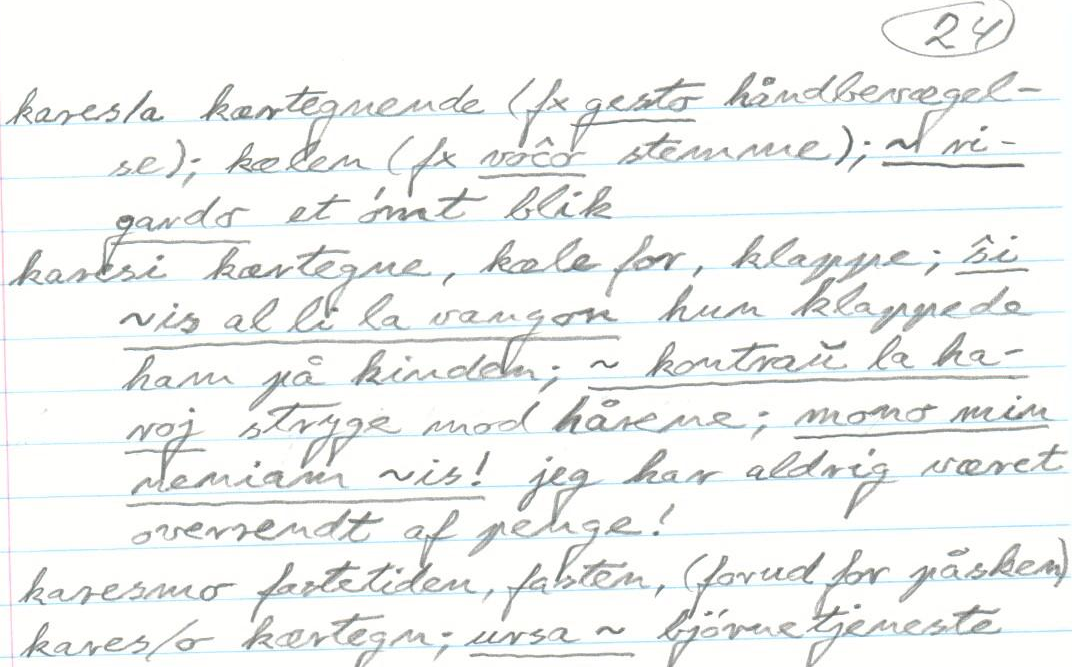
\includegraphics[width=10.5cm]{origino.png}
	
	{\selectlanguage{esperanto}\frenchspacing\itshape
	Parto de unu el la 731 pa\^goj de la mane skribita manuskripto}
	
\end{center}


{\selectlanguage{esperanto}\frenchspacing
Reveninte al Nepalo mi prezentis la manuskripton kaj la ideon al nepalaj
esperantistoj, kaj juna virino, Alinka Pokhrel, pretis preni la taskon,
kaj dum la sekva jaro \^si uzis pli ol 1500 laborhorojn por entajpi kaj
kontroli la 800 pa\^gojn, kontra\u{u} normala Nepala studenta salajro.
Danke al DEFA (Dana Esperanta Fervojista Asocio) ni ricevis malnovan
komputilon kun dana literumkontrolilo, kiu povis helpi \^sin literumi
preska\u{u} \^ciun danan vorton \^guste, kvankam \^si ne parolis la
danan:}


\begin{center}
\fbox{
\begin{minipage}{10.5cm}
\begin{alltt}
Pg. 24
\newline
\newline
kares/a k{\ae}rtegnende (fx \underline{gesto} h{\aa}ndbev{\ae}gelse); k{\ae}len (fx
\underline{voc\^{}o} stemme); \underline{\T{}rigardo} et {\o}mt blik
\newline
\newline
karesi\ \  k{\ae}rtegne, k{\ae}le for, klappe; \underline{s\^{}i \T{}is al li\ \ la vangon}
hun klappeda ham p{\aa}\ \ kinden; \underline{\T{} kontrau\^{} la karoj} stryge mod
h{\aa}rene; \underline{mono min neniam \T{}is!} jeg har aldrig v{\ae}ret overrendt
af penge!
\newline
\newline
karesmo\ \ \ \ \ \ \ \ \ \ fastetiden,  fasten, (forud for p{\aa}sken)
\newline
\newline
kares/o k{\ae}rtegn; \underline{ursa\T{}} bj{\o}rnetjenste
\end{alltt}
\end{minipage}
}

{\itshape La sama parto, post entajpo de Alinka}
\end{center}





{\selectlanguage{esperanto}\frenchspacing
\^Ciuj dosieroj de tiuj unuaj fazoj estas el\^suteblaj de la adreso:\\
\textit{http://javabog.dk/esperanto/dana\_vortaro\_bagger/}}

{\selectlanguage{esperanto}\frenchspacing
Dum 2010 mi ser\^cis kunlaborantojn kiuj volus helpi kontroli kaj
kompletigi la entajpitan manuskripton kaj trovis Jytte Sunek{\ae}r kaj
Peter Weide. Dum tri jaroj ni laboradis en nia libera tempo pri la
perfektigo de la manuskripto. Ni provis konservi la originalajn ideojn
kaj stilon de Preben, anka\u{u} en la literoj T, U, \u{U}, V kaj Z,
kiujn Peter Weide lerte ellaboris.}

{\selectlanguage{esperanto}\frenchspacing
Preben transdonis \^ciujn rajtojn pri la materialo al ni, .... kaj ni
nun \^satus pludoni tiujn rajtojn al vi:}

\section{Permesilo -- copyright}
{\selectlanguage{danish}
Undertegnende Preben Bagger overdrager hermed Jacob Nordfalk samtlige
rettigheder over det til ham tidligere udleverede materiale til
ESPERANTO-DANSK ordbog, og jeg fraskriver mig hermed alle rettigheder
til det n{\ae}vnte materiale.}

{\selectlanguage{danish}
Vi, Peter Weide, Jytte Sunek{\ae}r og Jacob Nordfalk, tillader hermed
enhver digital og fysisk brug, {\ae}ndring og reproduktion af ordbogen,
s{\aa} l{\ae}nge der er en angivelse af kilden.}

{\selectlanguage{danish}
Vi har arbejdet med st{\o}rste omhu. Alligevel vil l{\ae}seren finde
fejl. Vi vil v{\ae}re taknemmelige, hvis man informerer os, s{\aa} vi
kan rette fejlene. Forslag til nye ord er selvf{\o}lgelig er ogs{\aa}
velkomne. Vi beder om at anvendelser i trykte ordb{\o}ger venter, til
denne udgave er udsolgt.}

{\selectlanguage{esperanto}\frenchspacing
\textit{Tiu \^ci verko estas komuna hava\^{\j}o; vi rajtas uzi la verkon
}\foreignlanguage{danish}{\textit{kia}}\textit{ \^gi estas, komerce
a\u{u} nekomerce, plibonigi, \^san\^gi, adapti. Kion ajn. La sola
kondi\^co estas ke vi menci}\textit{u}\textit{ la fonton.}}

{\selectlanguage{esperanto}\frenchspacing
Ni laboris la\u{u}eble atenteme. Tamen eraroj trovi\^gos. Ni kun danko
akceptas informojn pri ili kaj la\u{u}eble rapide korektos ilin.
Memkompreneble anka\u{u} proponoj pri aldono de novaj vortoj estas
bonvenaj.}

{\selectlanguage{esperanto}\frenchspacing
Ni petas (ne postulas, sed petas) ke viaj uzoj ne rekte malgrandigu la
vendadon de tiu \^ci eldono, \^gis \^gi el\^cerpi\^gos.}


{\selectlanguage{danish}
Jacob Nordfalk, Peter Weide kaj Jytte Sunek{\ae}r}

{\selectlanguage{danish}
Valby, aprilo 2014.}


\begin{center}
	
\includegraphics[width=3cm]{permisilo.png}
\end{center}

\begin{center}
{\selectlanguage{esperanto}\frenchspacing\itshape
\^Ci tiu verko estas disponebla la\u{u} la permesilo\\
Krea Komuna\^{\j}o Atribuite 4.0 Tutmonda.\\
Vi povas legi la tutan permesilon \^ce:\\
http://creativecommons.org/licenses/by/4.0/deed.eo}
\end{center}


\end{document}
